\documentclass[a4paper]{book}
\usepackage{makeidx}
\usepackage{natbib}
\usepackage{graphicx}
\usepackage{multicol}
\usepackage{float}
\usepackage{listings}
\usepackage{color}
\usepackage{ifthen}
\usepackage[table]{xcolor}
\usepackage{textcomp}
\usepackage{alltt}
\usepackage{ifpdf}
\ifpdf
\usepackage[pdftex,
            pagebackref=true,
            colorlinks=true,
            linkcolor=blue,
            unicode
           ]{hyperref}
\else
\usepackage[ps2pdf,
            pagebackref=true,
            colorlinks=true,
            linkcolor=blue,
            unicode
           ]{hyperref}
\usepackage{pspicture}
\fi
\usepackage[utf8]{inputenc}
\usepackage{mathptmx}
\usepackage[scaled=.90]{helvet}
\usepackage{courier}
\usepackage{sectsty}
\usepackage[titles]{tocloft}
\usepackage{doxygen}
\lstset{language=C++,inputencoding=utf8,basicstyle=\footnotesize,breaklines=true,breakatwhitespace=true,tabsize=2,numbers=left }
\makeindex
\setcounter{tocdepth}{3}
\renewcommand{\footrulewidth}{0.4pt}
\renewcommand{\familydefault}{\sfdefault}
\hfuzz=15pt
\setlength{\emergencystretch}{15pt}
\hbadness=750
\tolerance=750
\begin{document}
\hypersetup{pageanchor=false,citecolor=blue}
\begin{titlepage}
\vspace*{7cm}
\begin{center}
{\Large \-Spacy }\\
\vspace*{1cm}
{\large \-Generated by Doxygen 1.7.6.1}\\
\vspace*{0.5cm}
{\small Sun Nov 20 2016 16:03:01}\\
\end{center}
\end{titlepage}
\clearemptydoublepage
\pagenumbering{roman}
\tableofcontents
\clearemptydoublepage
\pagenumbering{arabic}
\hypersetup{pageanchor=true,citecolor=blue}
\chapter{\-Spacy documentation}
\label{index}\hypertarget{index}{}\hypertarget{index_sec_intro}{}\section{Introduction}\label{index_sec_intro}
Vhat is a library that aims at
\begin{DoxyItemize}
\item providing an abstraction layer for the implementation of algorithms in a vector space setting (function space oriented algorithms)
\item providing a simple interface for sharing and comparing algorithms
\item having fun while developing algorithms
\item leaving you all freedom you want to implement your fancy algorithm (as long as you don\textquotesingle{}t violate the mathematical structure of vector spaces)
\end{DoxyItemize}\hypertarget{index_sec_overview}{}\section{Overview}\label{index_sec_overview}
The basis of Spacy is an abstraction layer for vector space settings. The interface of Spacy essentially builds on type erasure techniques. C++11/14-\/features such as \href{http://en.cppreference.com/w/cpp/language/value_category}{\tt R-\/values} are used, so make sure to use the compiler option -\/std=c++1y.\hypertarget{index_sub_concepts}{}\subsection{Main concepts}\label{index_sub_concepts}

\begin{DoxyItemize}
\item First there is a vector space class (\hyperlink{classSpacy_1_1VectorSpace}{Spacy\+::\+Vector\+Space}), which models a \hyperlink{namespaceSpacy_a0b66c8f2345b693504180dc7fb187958}{Banach space}  (X,$\vert$$\vert$.$\vert$$\vert$) or a \hyperlink{namespaceSpacy_a927756dd42df3e79c302df1f8f635b65}{Hilbert space}  (X,(.,.)). Thus, vector spaces provide access to a Norm and possibly a Scalar\+Product. Moreover, vector spaces can be related to each other as primal or dual spaces. Eventually they can generate vectors.
\item a \hyperlink{classSpacy_1_1Vector}{Vector} can be any class satisfying the Vector\+Concept, i.\+e. vectors must be vectors in a pure mathematical sense (almost).
\item an \hyperlink{classSpacy_1_1Operator}{Operator} (see Operator\+Concept) is a mapping vector spaces.
\item a \hyperlink{classSpacy_1_1Functional}{Functional} (see Functional\+Concept) is a mapping from a vector spaces into the space of real numbers $ \mathbb{R} $.
\item a \hyperlink{classSpacy_1_1LinearOperator}{Linear\+Operator}( see Linear\+Operator\+Concept) is a linear mapping between vector spaces that provides a solver for numerically evaluating its inverse. In addition linear operators satisfy the Vector\+Concept.
\end{DoxyItemize}\hypertarget{index_sec_usage_fenics}{}\section{Usage with F\+Enics}\label{index_sec_usage_fenics}
Examples for nonlinear P\+D\+Es and optimal control problems with \href{http://www.fenicsproject.org}{\tt F\+Eni\+CS} are given in Examples/\+F\+Eni\+CS.\hypertarget{index_sub_usage_fenics_pde}{}\subsection{Nonlinear P\+D\+Es with F\+Eni\+CS}\label{index_sub_usage_fenics_pde}
For an operator equation $A(x)=0$, discretized with \hyperlink{namespaceSpacy_1_1FEniCS}{F\+Eni\+CS} (\textquotesingle{}L\textquotesingle{} denoting the residual form and \textquotesingle{}a\textquotesingle{} the gradient form), simplest usage is as follows 
\begin{DoxyCode}
...
MyFEniCSExample::FunctionSpace V\{mesh\}
MyFEniCSExample::LinearForm L\{V\};
MyFEniCSExample::BilinearForm a\{V,V\};
...

\textcolor{comment}{// Create function space.}
auto domain = \hyperlink{group__FenicsGroup_ga8b67cb3d0188d2398625595b79e2fa6a}{Spacy::FEniCS::makeHilbertSpace}(V);

\textcolor{comment}{// Create operator mapping into the dual space of domain (which is, due to the Hilbert space structure,
       associated with domain itself).}
\textcolor{comment}{// You can also specify the range space if it differs from the dual space of domain}
\textcolor{comment}{// This is illustrated in the PDE example for Kaskade 7}
\textcolor{keyword}{auto} A = \hyperlink{group__KaskadeGroup_ga0e8d7d2c51e429e22561ef813fc97589}{Spacy::FEniCS::makeOperator}( L , a , domain );

\textcolor{comment}{// Solve with covariant Newton method with initial guess x0=0.}
\textcolor{keyword}{auto} x = \hyperlink{group__NewtonGroup_gad63424afc4a3a7f48368fd97d6279d56}{Spacy::covariantNewton}(A);


\textcolor{comment}{// Copy solution back to dolfin::Function.}
dolfin::Function u(V);
\hyperlink{group__FenicsGroup_ga7f43f0c660d0646adb031b453c536bb0}{Spacy::FEniCS::copy}(x,u);
...
\end{DoxyCode}
\hypertarget{index_sec_usage_kaskade}{}\section{Usage with Kaskade 7}\label{index_sec_usage_kaskade}
Examples for nonlinear P\+D\+Es and optimal control problems with \href{http://www.zib.de/projects/kaskade7-finite-element-toolbox}{\tt Kaskade 7} are given in Examples/\+Kaskade.\hypertarget{index_sub_usage_kaskade_pde}{}\subsection{Nonlinear P\+D\+Es with Kaskade 7}\label{index_sub_usage_kaskade_pde}
For an operator equation $A(x)=0$, discretized with \hyperlink{namespaceSpacy_1_1Kaskade}{Kaskade} 7 and with another scalar product, usage is as follows 
\begin{DoxyCode}
...
auto h1Space = Kaskade::FEFunctionSpace< ContinuousLagrangeMapper<double,LeafView> >\{(\} gridManager , 
      gridManager.grid().leafView() , order \};
...
auto variableSetDescription = VariableSetDescription\{ spaces , \{\textcolor{stringliteral}{"x"}\} \};
Functional F\{ ... \};
...

\textcolor{comment}{// Create domain and range space.}
auto domain = \hyperlink{group__VectorSpaceGroup_ga04d45446864bbf87770d02eade7b64cf}{Spacy::Kaskade::makeHilbertSpace}( space );
\textcolor{keyword}{auto} range  = \hyperlink{group__VectorSpaceGroup_ga04d45446864bbf87770d02eade7b64cf}{Spacy::Kaskade::makeHilbertSpace}( space );

\textcolor{comment}{// Create operator}
\textcolor{keyword}{auto} A = \hyperlink{group__KaskadeGroup_ga0e8d7d2c51e429e22561ef813fc97589}{Spacy::Kaskade::makeOperator}( F , domain , range );

\textcolor{comment}{// Set induced scalar product on domain space.}
\textcolor{keyword}{auto} x0 = domain.vector();
domain.setScalarProduct( InducedScalarProduct( A.linearization(x0) );

\textcolor{comment}{// Solve with covariant Newton method with initial guess x0=0.}
\textcolor{keyword}{auto} x = \hyperlink{group__NewtonGroup_gad63424afc4a3a7f48368fd97d6279d56}{Spacy::covariantNewton}( A , x0 );


\textcolor{comment}{// copy solution back to dolfin::Function}
\textcolor{keyword}{typename} VariableSetDescription::VariableSet u( variableSetDescription );
\hyperlink{namespaceSpacy_1_1Kaskade_afbbd7e385eda54f651c45b1c074d7bf9}{Spacy::Kaskade::copy}( x , u );
...
\end{DoxyCode}
 
\chapter{\-Todo \-List}
\label{todo}
\hypertarget{todo}{}

\begin{DoxyRefList}
\item[\label{todo__todo000001}%
\hypertarget{todo__todo000001}{}%
\-Class \hyperlink{classSpacy_1_1Generic_1_1VectorCreator}{\-Spacy\-:\-:\-Generic\-:\-:\-Vector\-Creator$<$ \-Vector\-Impl $>$} ]generalize vector creation 
\end{DoxyRefList}
\chapter{\-Module \-Index}
\section{Modules}
Here is a list of all modules\-:\begin{DoxyCompactList}
\item \contentsline{section}{Adapters}{\pageref{group__AdapterGroup}}{}
\begin{DoxyCompactList}
\item \contentsline{section}{deal.\-I\-I}{\pageref{group__dealIIGroup}}{}
\item \contentsline{section}{F\-Eni\-C\-S}{\pageref{group__FenicsGroup}}{}
\item \contentsline{section}{Kaskade7}{\pageref{group__KaskadeGroup}}{}
\item \contentsline{section}{Eigen}{\pageref{group__EigenGroup}}{}
\item \contentsline{section}{Generic}{\pageref{group__GenericGroup}}{}
\item \contentsline{section}{Scalar}{\pageref{group__ScalarGroup}}{}
\end{DoxyCompactList}
\item \contentsline{section}{Vector Spaces}{\pageref{group__VectorSpaceGroup}}{}
\begin{DoxyCompactList}
\item \contentsline{section}{Scalar}{\pageref{group__ScalarGroup}}{}
\item \contentsline{section}{Product Space}{\pageref{group__ProductSpaceGroup}}{}
\end{DoxyCompactList}
\item \contentsline{section}{Algorithms}{\pageref{group__AlgorithmGroup}}{}
\begin{DoxyCompactList}
\item \contentsline{section}{Newton Methods}{\pageref{group__NewtonGroup}}{}
\item \contentsline{section}{Conjugate Gradient Methods}{\pageref{group__CGGroup}}{}
\item \contentsline{section}{Composite Step Methods}{\pageref{group__CSGroup}}{}
\end{DoxyCompactList}
\item \contentsline{section}{@\{}{\pageref{group__KaskadeParabolicGroup}}{}
\end{DoxyCompactList}

\chapter{\-Namespace \-Index}
\section{Namespace List}
Here is a list of all documented namespaces with brief descriptions\+:\begin{DoxyCompactList}
\item\contentsline{section}{\hyperlink{namespaceSpacy}{Spacy} \\*Main namespace of the Spacy library }{\pageref{namespaceSpacy}}{}
\item\contentsline{section}{\hyperlink{namespaceSpacy_1_1CG}{Spacy\+::\+CG} \\*Conjugate gradient methods for convex and nonconvex problems (CG, Truncated CG, Regularized CG and Truncated Regularized CG) }{\pageref{namespaceSpacy_1_1CG}}{}
\item\contentsline{section}{\hyperlink{namespaceSpacy_1_1CG_1_1Termination}{Spacy\+::\+C\+G\+::\+Termination} \\*Termination criteria for conjugate gradient methods }{\pageref{namespaceSpacy_1_1CG_1_1Termination}}{}
\item\contentsline{section}{\hyperlink{namespaceSpacy_1_1CompositeStep}{Spacy\+::\+Composite\+Step} \\*Contains the affine covariant composite step method of \cite{Lubkoll2015}, \cite{Lubkoll2015a} }{\pageref{namespaceSpacy_1_1CompositeStep}}{}
\item\contentsline{section}{\hyperlink{namespaceSpacy_1_1FEniCS}{Spacy\+::\+F\+Eni\+CS} \\*Contains vector spaces, functionals and operators for \href{www.fenicsproject.org}{\tt F\+Eni\+CS} }{\pageref{namespaceSpacy_1_1FEniCS}}{}
\item\contentsline{section}{\hyperlink{namespaceSpacy_1_1Generic}{Spacy\+::\+Generic} \\*Contains generic implementations for easier definitions of vectors and a generic scalar product implementation }{\pageref{namespaceSpacy_1_1Generic}}{}
\item\contentsline{section}{\hyperlink{namespaceSpacy_1_1Kaskade}{Spacy\+::\+Kaskade} \\*Contains vector spaces, functionals and operators for \href{http://www.zib.de/projects/kaskade7-finite-element-toolbox}{\tt Kaskade7} }{\pageref{namespaceSpacy_1_1Kaskade}}{}
\item\contentsline{section}{\hyperlink{namespaceSpacy_1_1Mixin}{Spacy\+::\+Mixin} \\*Contains small independent components that are frequently used and can be added to classes via (multiple) inheritance }{\pageref{namespaceSpacy_1_1Mixin}}{}
\item\contentsline{section}{\hyperlink{namespaceSpacy_1_1Newton}{Spacy\+::\+Newton} \\*Newton methods, largely following \cite{Deuflhard2004} }{\pageref{namespaceSpacy_1_1Newton}}{}
\item\contentsline{section}{\hyperlink{namespaceSpacy_1_1Newton_1_1Damping}{Spacy\+::\+Newton\+::\+Damping} \\*Damping strategies for Newton\textquotesingle{}s method }{\pageref{namespaceSpacy_1_1Newton_1_1Damping}}{}
\item\contentsline{section}{\hyperlink{namespaceSpacy_1_1Newton_1_1Termination}{Spacy\+::\+Newton\+::\+Termination} \\*Termination criteria for Newton\textquotesingle{}s method }{\pageref{namespaceSpacy_1_1Newton_1_1Termination}}{}
\item\contentsline{section}{\hyperlink{namespaceSpacy_1_1Optional}{Spacy\+::\+Optional} }{\pageref{namespaceSpacy_1_1Optional}}{}
\item\contentsline{section}{\hyperlink{namespaceSpacy_1_1ProductSpace}{Spacy\+::\+Product\+Space} \\*A product space that supports distinction between primal and dual variables }{\pageref{namespaceSpacy_1_1ProductSpace}}{}
\item\contentsline{section}{\hyperlink{namespaceSpacy_1_1Rn}{Spacy\+::\+Rn} \\*Contains functionals and operators for finite dimensional vector space problems, based on \href{http://eigen.tuxfamily.org}{\tt Eigen} }{\pageref{namespaceSpacy_1_1Rn}}{}
\item\contentsline{section}{\hyperlink{namespaceSpacy_1_1Scalar}{Spacy\+::\+Scalar} \\*Contains functionals and operators for scalar problems }{\pageref{namespaceSpacy_1_1Scalar}}{}
\end{DoxyCompactList}

\chapter{\-Class \-Index}
\section{\-Class \-Hierarchy}
\-This inheritance list is sorted roughly, but not completely, alphabetically\-:\begin{DoxyCompactList}
\item \contentsline{section}{\-Spacy\-:\-:\-Adaptive\-Induced\-Scalar\-Product}{\pageref{classSpacy_1_1AdaptiveInducedScalarProduct}}{}
\item \contentsline{section}{\-Spacy\-:\-:\-Add\-Arithmetic\-Operators$<$ \-Derived $>$}{\pageref{classSpacy_1_1AddArithmeticOperators}}{}
\item \contentsline{section}{\-Spacy\-:\-:\-Add\-Arithmetic\-Operators$<$ \-Linear\-Operator $>$}{\pageref{classSpacy_1_1AddArithmeticOperators}}{}
\begin{DoxyCompactList}
\item \contentsline{section}{\-Spacy\-:\-:\-F\-Eni\-C\-S\-:\-:\-Linear\-Operator}{\pageref{classSpacy_1_1FEniCS_1_1LinearOperator}}{}
\item \contentsline{section}{\-Spacy\-:\-:\-Rn\-:\-:\-Linear\-Operator}{\pageref{classSpacy_1_1Rn_1_1LinearOperator}}{}
\item \contentsline{section}{\-Spacy\-:\-:\-Scalar\-:\-:\-Linear\-Operator}{\pageref{structSpacy_1_1Scalar_1_1LinearOperator}}{}
\end{DoxyCompactList}
\item \contentsline{section}{\-Spacy\-:\-:\-Add\-Arithmetic\-Operators$<$ \-Linear\-Operator$<$ \-Ansatz\-Variable\-Set\-Description, \-Test\-Variable\-Set\-Description $>$ $>$}{\pageref{classSpacy_1_1AddArithmeticOperators}}{}
\begin{DoxyCompactList}
\item \contentsline{section}{\-Spacy\-:\-:\-Kaskade\-:\-:\-Linear\-Operator$<$ \-Ansatz\-Variable\-Set\-Description, \-Test\-Variable\-Set\-Description $>$}{\pageref{classSpacy_1_1Kaskade_1_1LinearOperator}}{}
\end{DoxyCompactList}
\item \contentsline{section}{\-Spacy\-:\-:\-Add\-Arithmetic\-Operators$<$ \-Vector $>$}{\pageref{classSpacy_1_1AddArithmeticOperators}}{}
\begin{DoxyCompactList}
\item \contentsline{section}{\-Spacy\-:\-:\-F\-Eni\-C\-S\-:\-:\-Vector}{\pageref{classSpacy_1_1FEniCS_1_1Vector}}{}
\end{DoxyCompactList}
\item \contentsline{section}{\-Spacy\-:\-:\-Add\-Arithmetic\-Operators$<$ \-Vector$<$ \-Description $>$ $>$}{\pageref{classSpacy_1_1AddArithmeticOperators}}{}
\begin{DoxyCompactList}
\item \contentsline{section}{\-Spacy\-:\-:\-Kaskade\-:\-:\-Vector$<$ \-Description $>$}{\pageref{classSpacy_1_1Kaskade_1_1Vector}}{}
\end{DoxyCompactList}
\item \contentsline{section}{\-Spacy\-:\-:\-Add\-Arithmetic\-Operators$<$ \-Vector$<$ \-Vector\-Impl $>$ $>$}{\pageref{classSpacy_1_1AddArithmeticOperators}}{}
\begin{DoxyCompactList}
\item \contentsline{section}{\-Spacy\-:\-:\-Generic\-:\-:\-Vector$<$ \-Vector\-Impl $>$}{\pageref{classSpacy_1_1Generic_1_1Vector}}{}
\end{DoxyCompactList}
\item \contentsline{section}{\-Spacy\-:\-:\-Optional\-:\-:\-Mixin\-:\-:\-Attach$<$ \-Mixin, \-Mixins...$>$}{\pageref{structSpacy_1_1Optional_1_1Mixin_1_1Attach_3_01Mixin_00_01Mixins_8_8_8_4}}{}
\item \contentsline{section}{\-Spacy\-:\-:\-Optional\-:\-:\-Mixin\-:\-:\-Attach$<$$>$}{\pageref{structSpacy_1_1Optional_1_1Mixin_1_1Attach_3_4}}{}
\item \contentsline{section}{\-Spacy\-:\-:\-Product\-Space\-:\-:\-Basic\-Component\-View$<$ \-T $>$}{\pageref{structSpacy_1_1ProductSpace_1_1BasicComponentView}}{}
\item \contentsline{section}{\-Spacy\-:\-:\-Product\-Space\-:\-:\-Basic\-Component\-View$<$ const \-T $>$}{\pageref{structSpacy_1_1ProductSpace_1_1BasicComponentView_3_01const_01T_01_4}}{}
\item \contentsline{section}{\-Spacy\-:\-:deal\-I\-I\-:\-:\-Boundary\-Part$<$ dim $>$}{\pageref{structSpacy_1_1dealII_1_1BoundaryPart}}{}
\item \contentsline{section}{\-Spacy\-:\-:\-C1\-Functional}{\pageref{classSpacy_1_1C1Functional}}{}
\item \contentsline{section}{\-Spacy\-:\-:\-C1\-Operator}{\pageref{classSpacy_1_1C1Operator}}{}
\item \contentsline{section}{\-Spacy\-:\-:\-C2\-Functional}{\pageref{classSpacy_1_1C2Functional}}{}
\item \contentsline{section}{\-Spacy\-:\-:\-Call\-Of\-Undefined\-Function\-Exception}{\pageref{classSpacy_1_1CallOfUndefinedFunctionException}}{}
\item \contentsline{section}{\-Spacy\-:\-:\-Kaskade\-:\-:\-Coefficients\-To\-Variable\-Set$<$ n $>$}{\pageref{structSpacy_1_1Kaskade_1_1CoefficientsToVariableSet}}{}
\item \contentsline{section}{\-Spacy\-:\-:\-Kaskade\-:\-:\-Coefficients\-To\-Variable\-Set$<$-\/1 $>$}{\pageref{structSpacy_1_1Kaskade_1_1CoefficientsToVariableSet_3-1_01_4}}{}
\item \contentsline{section}{\-Spacy\-:\-:\-Mixin\-:\-:\-Contraction\-Rate}{\pageref{classSpacy_1_1Mixin_1_1ContractionRate}}{}
\begin{DoxyCompactList}
\item \contentsline{section}{\-Spacy\-:\-:\-Composite\-Step\-:\-:\-Affine\-Covariant\-Solver}{\pageref{classSpacy_1_1CompositeStep_1_1AffineCovariantSolver}}{}
\end{DoxyCompactList}
\item \contentsline{section}{\-Spacy\-:\-:deal\-I\-I\-:\-:\-Count\-Dims$<$ \-Variable\-Dim$<$ variable\-\_\-dims...$>$ $>$}{\pageref{structSpacy_1_1dealII_1_1CountDims_3_01VariableDim_3_01variable__dims_8_8_8_4_01_4}}{}
\item \contentsline{section}{\-Spacy\-:\-:deal\-I\-I\-:\-:\-Count\-Dims\-Impl$<$ variable\-\_\-dim $>$}{\pageref{structSpacy_1_1dealII_1_1CountDimsImpl_3_01variable__dim_01_4}}{}
\item \contentsline{section}{\-Spacy\-:\-:deal\-I\-I\-:\-:\-Count\-Dims\-Impl$<$ variable\-\_\-dim, variable\-\_\-dims...$>$}{\pageref{structSpacy_1_1dealII_1_1CountDimsImpl_3_01variable__dim_00_01variable__dims_8_8_8_4}}{}
\item \contentsline{section}{\-Spacy\-:\-:\-Scalar\-:\-:\-Cubic}{\pageref{classSpacy_1_1Scalar_1_1Cubic}}{}
\item \contentsline{section}{\-Spacy\-:\-:\-Composite\-Step\-:\-:\-Cubic\-Model}{\pageref{classSpacy_1_1CompositeStep_1_1CubicModel}}{}
\item \contentsline{section}{\-Spacy\-:\-:\-Mixin\-:\-:\-Decrease\-Condition}{\pageref{classSpacy_1_1Mixin_1_1DecreaseCondition}}{}
\begin{DoxyCompactList}
\item \contentsline{section}{\-Spacy\-:\-:\-Composite\-Step\-:\-:\-Affine\-Covariant\-Solver}{\pageref{classSpacy_1_1CompositeStep_1_1AffineCovariantSolver}}{}
\end{DoxyCompactList}
\item \contentsline{section}{\-Spacy\-:\-:\-Generic\-:\-:\-Default\-Interface$<$ \-Data $>$}{\pageref{structSpacy_1_1Generic_1_1DefaultInterface}}{}
\item \contentsline{section}{\-Spacy\-:\-:deal\-I\-I\-:\-:\-Detail\-:\-:\-Derivative\-Update$<$ dim, \-Variable\-Dims, row, column $>$}{\pageref{structSpacy_1_1dealII_1_1Detail_1_1DerivativeUpdate}}{}
\item \contentsline{section}{\-Spacy\-:\-:deal\-I\-I\-:\-:\-Detail\-:\-:\-Derivative\-Update$<$ dim, \-Variable\-Dims, row,-\/1 $>$}{\pageref{structSpacy_1_1dealII_1_1Detail_1_1DerivativeUpdate_3_01dim_00_01VariableDims_00_01row_00-1_01_4}}{}
\item \contentsline{section}{\-Spacy\-:\-:\-Optional\-:\-:\-Mixin\-:\-:\-Detach$<$ \-Mixin, \-Mixins...$>$}{\pageref{structSpacy_1_1Optional_1_1Mixin_1_1Detach_3_01Mixin_00_01Mixins_8_8_8_4}}{}
\item \contentsline{section}{\-Spacy\-:\-:\-Optional\-:\-:\-Mixin\-:\-:\-Detach$<$$>$}{\pageref{structSpacy_1_1Optional_1_1Mixin_1_1Detach_3_4}}{}
\item \contentsline{section}{\-Spacy\-:\-:\-Kaskade\-:\-:\-D\-L\-Y$<$ \-Definition, \-Ansatz\-Vars, \-Ansatz\-Vars\-Extension $>$}{\pageref{classSpacy_1_1Kaskade_1_1DLY}}{}
\item \contentsline{section}{\-Spacy\-:\-:\-Dynamic\-C1\-Operator}{\pageref{classSpacy_1_1DynamicC1Operator}}{}
\item \contentsline{section}{\-Spacy\-:\-:\-Dynamic\-Linear\-Operator}{\pageref{classSpacy_1_1DynamicLinearOperator}}{}
\item \contentsline{section}{\-Spacy\-:\-:\-Dynamic\-Operator}{\pageref{classSpacy_1_1DynamicOperator}}{}
\item \contentsline{section}{\-Spacy\-:\-:\-Generic\-:\-:\-Euclidean\-Scalar\-Product}{\pageref{classSpacy_1_1Generic_1_1EuclideanScalarProduct}}{}
\item \contentsline{section}{\-Spacy\-:\-:\-Functional}{\pageref{classSpacy_1_1Functional}}{}
\item \contentsline{section}{\-Spacy\-:\-:\-Functional\-Base}{\pageref{classSpacy_1_1FunctionalBase}}{}
\begin{DoxyCompactList}
\item \contentsline{section}{\-Spacy\-:\-:deal\-I\-I\-:\-:\-C2\-Fun\-G\-Functional$<$ \-Fun\-G\-Functional, dim, \-Variable\-Dim$<$ variable\-\_\-dims...$>$ $>$}{\pageref{classSpacy_1_1dealII_1_1C2FunGFunctional_3_01FunGFunctional_00_01dim_00_01VariableDim_3_01variable__dims_8_8_8_4_01_4}}{}
\item \contentsline{section}{\-Spacy\-:\-:\-F\-Eni\-C\-S\-:\-:\-C2\-Functional$<$ \-F, \-D\-F, \-D\-D\-F $>$}{\pageref{classSpacy_1_1FEniCS_1_1C2Functional}}{}
\item \contentsline{section}{\-Spacy\-:\-:\-Kaskade\-:\-:\-C2\-Functional$<$ \-Functional\-Definition $>$}{\pageref{classSpacy_1_1Kaskade_1_1C2Functional}}{}
\item \contentsline{section}{\-Spacy\-:\-:\-Rn\-:\-:\-C2\-Functional}{\pageref{classSpacy_1_1Rn_1_1C2Functional}}{}
\item \contentsline{section}{\-Spacy\-:\-:\-Rn\-:\-:\-Composite\-Step\-Functional$<$ role $>$}{\pageref{classSpacy_1_1Rn_1_1CompositeStepFunctional}}{}
\item \contentsline{section}{\-Spacy\-:\-:\-Scalar\-:\-:\-C2\-Functional}{\pageref{classSpacy_1_1Scalar_1_1C2Functional}}{}
\end{DoxyCompactList}
\item \contentsline{section}{\-Spacy\-:\-:deal\-I\-I\-:\-:\-Detail\-:\-:\-Functional\-Update$<$ dim, \-Variable\-Dims, id $>$}{\pageref{structSpacy_1_1dealII_1_1Detail_1_1FunctionalUpdate}}{}
\item \contentsline{section}{\-Spacy\-:\-:deal\-I\-I\-:\-:\-Detail\-:\-:\-Functional\-Update$<$ dim, \-Variable\-Dims,-\/1 $>$}{\pageref{structSpacy_1_1dealII_1_1Detail_1_1FunctionalUpdate_3_01dim_00_01VariableDims_00-1_01_4}}{}
\item \contentsline{section}{\-Spacy\-:\-:\-Generic\-Exception}{\pageref{classSpacy_1_1GenericException}}{}
\begin{DoxyCompactList}
\item \contentsline{section}{\-Spacy\-:\-:\-Incompatible\-Space\-Exception}{\pageref{classSpacy_1_1IncompatibleSpaceException}}{}
\end{DoxyCompactList}
\item \contentsline{section}{\-Spacy\-:\-:deal\-I\-I\-:\-:\-Get\-Boundary\-Map$<$ dim, \-Variable\-Dims, id $>$}{\pageref{structSpacy_1_1dealII_1_1GetBoundaryMap}}{}
\item \contentsline{section}{\-Spacy\-:\-:deal\-I\-I\-:\-:\-Get\-Boundary\-Map$<$ dim, \-Variable\-Dims,-\/1 $>$}{\pageref{structSpacy_1_1dealII_1_1GetBoundaryMap_3_01dim_00_01VariableDims_00-1_01_4}}{}
\item \contentsline{section}{\-Spacy\-:\-:deal\-I\-I\-:\-:\-Get\-Dim$<$ id, \-Components, id\-\_\-in\-\_\-component $>$}{\pageref{structSpacy_1_1dealII_1_1GetDim}}{}
\item \contentsline{section}{\-Spacy\-:\-:deal\-I\-I\-:\-:\-Get\-Dim$<$ id, \-Components$<$ dim, ids...$>$, id\-\_\-in\-\_\-component $>$}{\pageref{structSpacy_1_1dealII_1_1GetDim_3_01id_00_01Components_3_01dim_00_01ids_8_8_8_4_00_01id__in__component_01_4}}{}
\item \contentsline{section}{\-Spacy\-:\-:deal\-I\-I\-:\-:\-Get\-Finite\-Element$<$ dim, \-Variable\-Dims, id $>$}{\pageref{structSpacy_1_1dealII_1_1GetFiniteElement}}{}
\item \contentsline{section}{\-Spacy\-:\-:deal\-I\-I\-:\-:\-Get\-Finite\-Element\-System$<$ dim, \-Variable\-Dim$<$ variable\-\_\-dims...$>$ $>$}{\pageref{structSpacy_1_1dealII_1_1GetFiniteElementSystem_3_01dim_00_01VariableDim_3_01variable__dims_8_8_8_4_01_4}}{}
\item \contentsline{section}{\-Spacy\-:\-:\-Generic\-:\-:\-Detail\-:\-:\-Has\-Static\-Mem\-Fn\-\_\-\-Zero$<$ \-T, class $>$}{\pageref{structSpacy_1_1Generic_1_1Detail_1_1HasStaticMemFn__Zero}}{}
\item \contentsline{section}{\-Spacy\-:\-:\-Generic\-:\-:\-Detail\-:\-:\-Has\-Static\-Mem\-Fn\-\_\-\-Zero$<$ \-T, voider$<$ \-Try\-Static\-Mem\-Fn\-\_\-\-Zero$<$ \-T $>$ $>$ $>$}{\pageref{structSpacy_1_1Generic_1_1Detail_1_1HasStaticMemFn__Zero_3_01T_00_01voider_3_01TryStaticMemFn__Zero_3_01T_01_4_01_4_01_4}}{}
\item \contentsline{section}{\-Spacy\-:\-:\-Hilbert\-Space\-Norm}{\pageref{classSpacy_1_1HilbertSpaceNorm}}{}
\item \contentsline{section}{\-Spacy\-:\-:\-Generic\-:\-:\-Ignore}{\pageref{structSpacy_1_1Generic_1_1Ignore}}{}
\item \contentsline{section}{\-Spacy\-:\-:\-Indefinite\-Linear\-Solver}{\pageref{classSpacy_1_1IndefiniteLinearSolver}}{}
\item \contentsline{section}{\-Spacy\-:\-:\-Induced\-Scalar\-Product}{\pageref{classSpacy_1_1InducedScalarProduct}}{}
\item \contentsline{section}{\-Spacy\-:\-:deal\-I\-I\-:\-:\-Init\-Blocks$<$ dim, \-Variable\-Dims, row, column $>$}{\pageref{structSpacy_1_1dealII_1_1InitBlocks}}{}
\item \contentsline{section}{\-Spacy\-:\-:deal\-I\-I\-:\-:\-Init\-Blocks$<$ dim, \-Variable\-Dims, row,-\/1 $>$}{\pageref{structSpacy_1_1dealII_1_1InitBlocks_3_01dim_00_01VariableDims_00_01row_00-1_01_4}}{}
\item \contentsline{section}{\-Spacy\-:\-:deal\-I\-I\-:\-:\-Init\-Block\-Vector$<$ dim, \-Variable\-Dims, id, is\-\_\-product\-\_\-space $>$}{\pageref{structSpacy_1_1dealII_1_1InitBlockVector}}{}
\item \contentsline{section}{\-Spacy\-:\-:deal\-I\-I\-:\-:\-Init\-Block\-Vector$<$ dim, \-Variable\-Dims, 0, false $>$}{\pageref{structSpacy_1_1dealII_1_1InitBlockVector_3_01dim_00_01VariableDims_00_010_00_01false_01_4}}{}
\item \contentsline{section}{\-Spacy\-:\-:deal\-I\-I\-:\-:\-Init\-Block\-Vector$<$ dim, \-Variable\-Dims,-\/1, is\-\_\-product\-\_\-space $>$}{\pageref{structSpacy_1_1dealII_1_1InitBlockVector_3_01dim_00_01VariableDims_00-1_00_01is__product__space_01_4}}{}
\item \contentsline{section}{\-Spacy\-:\-:deal\-I\-I\-:\-:\-Init\-Sparsity\-Pattern$<$ dim, \-Variable\-Dims, size $>$}{\pageref{structSpacy_1_1dealII_1_1InitSparsityPattern}}{}
\item \contentsline{section}{\-Spacy\-:\-:deal\-I\-I\-:\-:\-Init\-Sparsity\-Pattern$<$ dim, \-Variable\-Dims, 1 $>$}{\pageref{structSpacy_1_1dealII_1_1InitSparsityPattern_3_01dim_00_01VariableDims_00_011_01_4}}{}
\item \contentsline{section}{\-Spacy\-:\-:\-Exception\-:\-:\-Invalid\-Argument}{\pageref{classSpacy_1_1Exception_1_1InvalidArgument}}{}
\item \contentsline{section}{\-Spacy\-:\-:\-F\-Eni\-C\-S\-:\-:l2\-Product}{\pageref{classSpacy_1_1FEniCS_1_1l2Product}}{}
\item \contentsline{section}{\-Spacy\-:\-:\-Kaskade\-:\-:l2\-Product$<$ \-Description $>$}{\pageref{classSpacy_1_1Kaskade_1_1l2Product}}{}
\item \contentsline{section}{\-Spacy\-:\-:\-Linear\-Operator}{\pageref{classSpacy_1_1LinearOperator}}{}
\item \contentsline{section}{\-Spacy\-:\-:\-F\-Eni\-C\-S\-:\-:\-Linear\-Operator\-Creator}{\pageref{classSpacy_1_1FEniCS_1_1LinearOperatorCreator}}{}
\item \contentsline{section}{\-Spacy\-:\-:deal\-I\-I\-:\-:\-Linear\-Operator\-Creator}{\pageref{structSpacy_1_1dealII_1_1LinearOperatorCreator}}{}
\item \contentsline{section}{\-Spacy\-:\-:\-Kaskade\-:\-:\-Linear\-Operator\-Creator$<$ \-Ansatz\-Variable\-Set\-Description, \-Test\-Variable\-Set\-Description $>$}{\pageref{classSpacy_1_1Kaskade_1_1LinearOperatorCreator}}{}
\item \contentsline{section}{\-Spacy\-:\-:\-Rn\-:\-:\-Linear\-Solver}{\pageref{classSpacy_1_1Rn_1_1LinearSolver}}{}
\item \contentsline{section}{\-Spacy\-:\-:\-Scalar\-:\-:\-Linear\-Solver}{\pageref{classSpacy_1_1Scalar_1_1LinearSolver}}{}
\item \contentsline{section}{\-Spacy\-:\-:deal\-I\-I\-:\-:\-Detail\-:\-:\-Local\-Assembly\-Base$<$ dim, row, row\-\_\-dim, column, column\-\_\-dim $>$}{\pageref{structSpacy_1_1dealII_1_1Detail_1_1LocalAssemblyBase}}{}
\begin{DoxyCompactList}
\item \contentsline{section}{\-Spacy\-:\-:deal\-I\-I\-:\-:\-Detail\-:\-:\-Local\-Fun\-G\-Functional\-Derivative\-Assembly$<$ dim, \-Components, row, column, row\-\_\-dim, column\-\_\-dim $>$}{\pageref{structSpacy_1_1dealII_1_1Detail_1_1LocalFunGFunctionalDerivativeAssembly}}{}
\item \contentsline{section}{\-Spacy\-:\-:deal\-I\-I\-:\-:\-Detail\-:\-:\-Local\-Fun\-G\-Operator\-Assembly$<$ dim, \-Components, row, column, row\-\_\-dim, column\-\_\-dim $>$}{\pageref{structSpacy_1_1dealII_1_1Detail_1_1LocalFunGOperatorAssembly}}{}
\end{DoxyCompactList}
\item \contentsline{section}{\-Spacy\-:\-:deal\-I\-I\-:\-:\-Detail\-:\-:\-Local\-Assembly\-Base$<$ dim, id, 1 $>$}{\pageref{structSpacy_1_1dealII_1_1Detail_1_1LocalAssemblyBase}}{}
\begin{DoxyCompactList}
\item \contentsline{section}{\-Spacy\-:\-:deal\-I\-I\-:\-:\-Detail\-:\-:\-Local\-Fun\-G\-Functional\-Value\-Assembly$<$ dim, \-Components, id, 1 $>$}{\pageref{structSpacy_1_1dealII_1_1Detail_1_1LocalFunGFunctionalValueAssembly_3_01dim_00_01Components_00_01id_00_011_01_4}}{}
\end{DoxyCompactList}
\item \contentsline{section}{\-Spacy\-:\-:deal\-I\-I\-:\-:\-Detail\-:\-:\-Local\-Assembly\-Base$<$ dim, id, dim $>$}{\pageref{structSpacy_1_1dealII_1_1Detail_1_1LocalAssemblyBase}}{}
\begin{DoxyCompactList}
\item \contentsline{section}{\-Spacy\-:\-:deal\-I\-I\-:\-:\-Detail\-:\-:\-Local\-Fun\-G\-Functional\-Value\-Assembly$<$ dim, \-Components, id, dim $>$}{\pageref{structSpacy_1_1dealII_1_1Detail_1_1LocalFunGFunctionalValueAssembly_3_01dim_00_01Components_00_01id_00_01dim_01_4}}{}
\end{DoxyCompactList}
\item \contentsline{section}{\-Spacy\-:\-:\-Logger$<$ \-T, class $>$}{\pageref{structSpacy_1_1Logger}}{}
\item \contentsline{section}{\-Spacy\-:\-:\-Mixin\-:\-:\-Mixin\-Connection$<$ \-Impl $>$}{\pageref{classSpacy_1_1Mixin_1_1MixinConnection}}{}
\item \contentsline{section}{\-Spacy\-:\-:\-Mixin\-:\-:\-Mixin\-Connection$<$ \-Eps $>$}{\pageref{classSpacy_1_1Mixin_1_1MixinConnection}}{}
\begin{DoxyCompactList}
\item \contentsline{section}{\-Spacy\-:\-:\-Mixin\-:\-:\-Eps}{\pageref{classSpacy_1_1Mixin_1_1Eps}}{}
\begin{DoxyCompactList}
\item \contentsline{section}{\-Spacy\-:\-:\-A\-C\-R\-:\-:\-A\-C\-R\-Solver}{\pageref{classSpacy_1_1ACR_1_1ACRSolver}}{}
\item \contentsline{section}{\-Spacy\-:\-:\-Algorithm\-:\-:\-Trust\-Region\-Solver}{\pageref{classSpacy_1_1Algorithm_1_1TrustRegionSolver}}{}
\item \contentsline{section}{\-Spacy\-:\-:\-C\-G\-:\-:\-Linear\-Solver}{\pageref{classSpacy_1_1CG_1_1LinearSolver}}{}
\item \contentsline{section}{\-Spacy\-:\-:\-C\-G\-:\-:\-Solver}{\pageref{classSpacy_1_1CG_1_1Solver}}{}
\item \contentsline{section}{\-Spacy\-:\-:\-C\-G\-:\-:\-Termination\-:\-:\-Strakos\-Tichy\-Energy\-Error}{\pageref{classSpacy_1_1CG_1_1Termination_1_1StrakosTichyEnergyError}}{}
\item \contentsline{section}{\-Spacy\-:\-:\-Composite\-Step\-:\-:\-Affine\-Covariant\-Solver}{\pageref{classSpacy_1_1CompositeStep_1_1AffineCovariantSolver}}{}
\item \contentsline{section}{\-Spacy\-:\-:\-Damping\-Factor}{\pageref{classSpacy_1_1DampingFactor}}{}
\item \contentsline{section}{\-Spacy\-:\-:\-Kaskade\-:\-:\-C2\-Functional$<$ \-Functional\-Definition $>$}{\pageref{classSpacy_1_1Kaskade_1_1C2Functional}}{}
\item \contentsline{section}{\-Spacy\-:\-:\-Kaskade\-:\-:\-Lagrange\-:\-:\-C\-G\-Creator$<$ \-Functional\-Definition, state\-Id, control\-Id, adjoint\-Id $>$}{\pageref{classSpacy_1_1Kaskade_1_1Lagrange_1_1CGCreator}}{}
\item \contentsline{section}{\-Spacy\-:\-:\-Lipschitz\-Constant}{\pageref{classSpacy_1_1LipschitzConstant}}{}
\item \contentsline{section}{\-Spacy\-:\-:\-Newton\-:\-:\-Damping\-:\-:\-Affine\-Contravariant}{\pageref{classSpacy_1_1Newton_1_1Damping_1_1AffineContravariant}}{}
\item \contentsline{section}{\-Spacy\-:\-:\-Newton\-:\-:\-Damping\-:\-:\-Affine\-Covariant}{\pageref{classSpacy_1_1Newton_1_1Damping_1_1AffineCovariant}}{}
\item \contentsline{section}{\-Spacy\-:\-:\-Newton\-:\-:\-Parameter}{\pageref{structSpacy_1_1Newton_1_1Parameter}}{}
\item \contentsline{section}{\-Spacy\-:\-:\-Newton\-:\-:\-Termination\-:\-:\-Affine\-Contravariant}{\pageref{classSpacy_1_1Newton_1_1Termination_1_1AffineContravariant}}{}
\item \contentsline{section}{\-Spacy\-:\-:\-Newton\-:\-:\-Termination\-:\-:\-Affine\-Covariant}{\pageref{classSpacy_1_1Newton_1_1Termination_1_1AffineCovariant}}{}
\item \contentsline{section}{\-Spacy\-:\-:\-Parameter}{\pageref{classSpacy_1_1Parameter}}{}
\item \contentsline{section}{\-Spacy\-:\-:\-Vector\-Space}{\pageref{classSpacy_1_1VectorSpace}}{}
\end{DoxyCompactList}
\end{DoxyCompactList}
\item \contentsline{section}{\-Spacy\-:\-:\-Mixin\-:\-:\-Mixin\-Connection$<$ \-Regularity\-Test $>$}{\pageref{classSpacy_1_1Mixin_1_1MixinConnection}}{}
\begin{DoxyCompactList}
\item \contentsline{section}{\-Spacy\-:\-:\-Mixin\-:\-:\-Regularity\-Test}{\pageref{classSpacy_1_1Mixin_1_1RegularityTest}}{}
\begin{DoxyCompactList}
\item \contentsline{section}{\-Spacy\-:\-:\-Composite\-Step\-:\-:\-Affine\-Covariant\-Solver}{\pageref{classSpacy_1_1CompositeStep_1_1AffineCovariantSolver}}{}
\item \contentsline{section}{\-Spacy\-:\-:\-Newton\-:\-:\-Damping\-:\-:\-Affine\-Contravariant}{\pageref{classSpacy_1_1Newton_1_1Damping_1_1AffineContravariant}}{}
\item \contentsline{section}{\-Spacy\-:\-:\-Newton\-:\-:\-Damping\-:\-:\-Affine\-Covariant}{\pageref{classSpacy_1_1Newton_1_1Damping_1_1AffineCovariant}}{}
\item \contentsline{section}{\-Spacy\-:\-:\-Newton\-:\-:\-Parameter}{\pageref{structSpacy_1_1Newton_1_1Parameter}}{}
\end{DoxyCompactList}
\end{DoxyCompactList}
\item \contentsline{section}{\-Spacy\-:\-:\-Mixin\-:\-:\-Mixin\-Connection$<$ \-Verbosity $>$}{\pageref{classSpacy_1_1Mixin_1_1MixinConnection}}{}
\begin{DoxyCompactList}
\item \contentsline{section}{\-Spacy\-:\-:\-Mixin\-:\-:\-Verbosity}{\pageref{classSpacy_1_1Mixin_1_1Verbosity}}{}
\begin{DoxyCompactList}
\item \contentsline{section}{\-Spacy\-:\-:\-A\-C\-R\-:\-:\-A\-C\-R\-Solver}{\pageref{classSpacy_1_1ACR_1_1ACRSolver}}{}
\item \contentsline{section}{\-Spacy\-:\-:\-C\-G\-:\-:\-Linear\-Solver}{\pageref{classSpacy_1_1CG_1_1LinearSolver}}{}
\item \contentsline{section}{\-Spacy\-:\-:\-C\-G\-:\-:\-Solver}{\pageref{classSpacy_1_1CG_1_1Solver}}{}
\item \contentsline{section}{\-Spacy\-:\-:\-C\-G\-:\-:\-Termination\-:\-:\-Strakos\-Tichy\-Energy\-Error}{\pageref{classSpacy_1_1CG_1_1Termination_1_1StrakosTichyEnergyError}}{}
\item \contentsline{section}{\-Spacy\-:\-:\-Composite\-Step\-:\-:\-Affine\-Covariant\-Solver}{\pageref{classSpacy_1_1CompositeStep_1_1AffineCovariantSolver}}{}
\item \contentsline{section}{\-Spacy\-:\-:\-Kaskade\-:\-:\-Lagrange\-:\-:\-C\-G\-Creator$<$ \-Functional\-Definition, state\-Id, control\-Id, adjoint\-Id $>$}{\pageref{classSpacy_1_1Kaskade_1_1Lagrange_1_1CGCreator}}{}
\item \contentsline{section}{\-Spacy\-:\-:\-Parameter}{\pageref{classSpacy_1_1Parameter}}{}
\end{DoxyCompactList}
\end{DoxyCompactList}
\item \contentsline{section}{\-Spacy\-:\-:\-Generic\-:\-:\-No\-Data}{\pageref{structSpacy_1_1Generic_1_1NoData}}{}
\item \contentsline{section}{\-Spacy\-:\-:\-Newton\-:\-:\-Damping\-:\-:\-None}{\pageref{classSpacy_1_1Newton_1_1Damping_1_1None}}{}
\item \contentsline{section}{\-Spacy\-:\-:\-Product\-Space\-:\-:\-Norm}{\pageref{classSpacy_1_1ProductSpace_1_1Norm}}{}
\item \contentsline{section}{\-Spacy\-:\-:\-Exception\-:\-:\-Not\-Converged}{\pageref{structSpacy_1_1Exception_1_1NotConverged}}{}
\item \contentsline{section}{\-Spacy\-:\-:\-Operator}{\pageref{classSpacy_1_1Operator}}{}
\item \contentsline{section}{\-Spacy\-:\-:\-Operator\-Base}{\pageref{classSpacy_1_1OperatorBase}}{}
\begin{DoxyCompactList}
\item \contentsline{section}{\-Spacy\-:\-:\-C\-G\-:\-:\-Linear\-Solver}{\pageref{classSpacy_1_1CG_1_1LinearSolver}}{}
\item \contentsline{section}{\-Spacy\-:\-:\-C\-G\-:\-:\-Triangular\-State\-Constraint\-Preconditioner}{\pageref{classSpacy_1_1CG_1_1TriangularStateConstraintPreconditioner}}{}
\item \contentsline{section}{\-Spacy\-:\-:deal\-I\-I\-:\-:\-C1\-Fun\-G\-Operator$<$ \-Fun\-G\-Operator, dim, \-Variable\-Dim$<$ variable\-\_\-dims...$>$ $>$}{\pageref{classSpacy_1_1dealII_1_1C1FunGOperator_3_01FunGOperator_00_01dim_00_01VariableDim_3_01variable__dims_8_8_8_4_01_4}}{}
\item \contentsline{section}{\-Spacy\-:\-:deal\-I\-I\-:\-:\-C\-G\-Solver$<$ dim $>$}{\pageref{classSpacy_1_1dealII_1_1CGSolver}}{}
\item \contentsline{section}{\-Spacy\-:\-:deal\-I\-I\-:\-:\-Linear\-Operator$<$ dim, \-Variable\-Dims $>$}{\pageref{classSpacy_1_1dealII_1_1LinearOperator}}{}
\item \contentsline{section}{\-Spacy\-:\-:deal\-I\-I\-:\-:\-U\-M\-F\-Pack\-Solver$<$ \-Variable\-Dims $>$}{\pageref{classSpacy_1_1dealII_1_1UMFPackSolver}}{}
\item \contentsline{section}{\-Spacy\-:\-:\-F\-Eni\-C\-S\-:\-:\-C1\-Operator$<$ \-Residual\-Form, \-Jacobian\-Form $>$}{\pageref{classSpacy_1_1FEniCS_1_1C1Operator}}{}
\item \contentsline{section}{\-Spacy\-:\-:\-F\-Eni\-C\-S\-:\-:\-Linear\-Operator}{\pageref{classSpacy_1_1FEniCS_1_1LinearOperator}}{}
\item \contentsline{section}{\-Spacy\-:\-:\-F\-Eni\-C\-S\-:\-:\-L\-U\-Solver}{\pageref{classSpacy_1_1FEniCS_1_1LUSolver}}{}
\item \contentsline{section}{\-Spacy\-:\-:\-F\-Eni\-C\-S\-:\-:\-Transposed\-L\-U\-Solver}{\pageref{classSpacy_1_1FEniCS_1_1TransposedLUSolver}}{}
\item \contentsline{section}{\-Spacy\-:\-:\-Generic\-:\-:\-Linear\-Operator\-Creator$<$ \-Linear\-Operator $>$}{\pageref{classSpacy_1_1Generic_1_1LinearOperatorCreator}}{}
\begin{DoxyCompactList}
\item \contentsline{section}{\-Spacy\-:\-:\-Rn\-:\-:\-Linear\-Operator\-Creator}{\pageref{structSpacy_1_1Rn_1_1LinearOperatorCreator}}{}
\end{DoxyCompactList}
\item \contentsline{section}{\-Spacy\-:\-:\-Kaskade\-:\-:\-C1\-Operator$<$ \-Operator\-Definition $>$}{\pageref{classSpacy_1_1Kaskade_1_1C1Operator}}{}
\item \contentsline{section}{\-Spacy\-:\-:\-Kaskade\-:\-:\-Direct\-Solver$<$ \-Kaskade\-Operator, \-Ansatz\-Variable\-Description, \-Test\-Variable\-Description $>$}{\pageref{classSpacy_1_1Kaskade_1_1DirectSolver}}{}
\item \contentsline{section}{\-Spacy\-:\-:\-Kaskade\-:\-:\-Dynamic\-C1\-Operator$<$ \-Operator\-Definition, \-Mass\-Definition $>$}{\pageref{classSpacy_1_1Kaskade_1_1DynamicC1Operator}}{}
\item \contentsline{section}{\-Spacy\-:\-:\-Kaskade\-:\-:\-Linear\-Operator$<$ \-Ansatz\-Variable\-Set\-Description, \-Test\-Variable\-Set\-Description $>$}{\pageref{classSpacy_1_1Kaskade_1_1LinearOperator}}{}
\item \contentsline{section}{\-Spacy\-:\-:\-Kaskade\-:\-:\-Operator$<$ \-Operator\-Definition $>$}{\pageref{classSpacy_1_1Kaskade_1_1Operator}}{}
\item \contentsline{section}{\-Spacy\-:\-:\-Rn\-:\-:\-C1\-Operator}{\pageref{classSpacy_1_1Rn_1_1C1Operator}}{}
\item \contentsline{section}{\-Spacy\-:\-:\-Rn\-:\-:\-Linear\-Operator}{\pageref{classSpacy_1_1Rn_1_1LinearOperator}}{}
\item \contentsline{section}{\-Spacy\-:\-:\-Scalar\-:\-:\-C1\-Operator}{\pageref{classSpacy_1_1Scalar_1_1C1Operator}}{}
\item \contentsline{section}{\-Spacy\-:\-:\-Scalar\-:\-:\-Linear\-Operator}{\pageref{structSpacy_1_1Scalar_1_1LinearOperator}}{}
\end{DoxyCompactList}
\item \contentsline{section}{\-Spacy\-:\-:deal\-I\-I\-:\-:\-Detail\-:\-:\-Operator\-Update$<$ dim, \-Variable\-Dims, row, column $>$}{\pageref{structSpacy_1_1dealII_1_1Detail_1_1OperatorUpdate}}{}
\item \contentsline{section}{\-Spacy\-:\-:deal\-I\-I\-:\-:\-Detail\-:\-:\-Operator\-Update$<$ dim, \-Variable\-Dims, row,-\/1 $>$}{\pageref{structSpacy_1_1dealII_1_1Detail_1_1OperatorUpdate_3_01dim_00_01VariableDims_00_01row_00-1_01_4}}{}
\item \contentsline{section}{\-Spacy\-:\-:\-Primal\-Induced\-Scalar\-Product}{\pageref{classSpacy_1_1PrimalInducedScalarProduct}}{}
\item \contentsline{section}{\-Spacy\-:\-:\-Log\-:\-:\-Printer}{\pageref{classSpacy_1_1Log_1_1Printer}}{}
\item \contentsline{section}{\-Spacy\-:\-:\-Scalar\-:\-:\-Quadratic}{\pageref{classSpacy_1_1Scalar_1_1Quadratic}}{}
\item \contentsline{section}{\-Spacy\-:\-:\-Regularity\-Test\-Failed\-Exception}{\pageref{classSpacy_1_1RegularityTestFailedException}}{}
\item \contentsline{section}{\-Spacy\-:\-:\-Product\-Space\-:\-:\-Scalar\-Product}{\pageref{classSpacy_1_1ProductSpace_1_1ScalarProduct}}{}
\item \contentsline{section}{\-Spacy\-:\-:\-Optional\-:\-:\-Mixin\-:\-:\-Single\-Attach$<$ \-Callee, \-To\-Attach, \-Mixin, valid $>$}{\pageref{structSpacy_1_1Optional_1_1Mixin_1_1SingleAttach}}{}
\item \contentsline{section}{\-Spacy\-:\-:\-Optional\-:\-:\-Mixin\-:\-:\-Single\-Attach$<$ \-Callee, \-To\-Attach, \-Mixin, false $>$}{\pageref{structSpacy_1_1Optional_1_1Mixin_1_1SingleAttach_3_01Callee_00_01ToAttach_00_01Mixin_00_01false_01_4}}{}
\item \contentsline{section}{\-Spacy\-:\-:\-Optional\-:\-:\-Mixin\-:\-:\-Single\-Detach$<$ \-Callee, \-To\-Detach, \-Mixin, valid $>$}{\pageref{structSpacy_1_1Optional_1_1Mixin_1_1SingleDetach}}{}
\item \contentsline{section}{\-Spacy\-:\-:\-Optional\-:\-:\-Mixin\-:\-:\-Single\-Detach$<$ \-Callee, \-To\-Detach, \-Mixin, false $>$}{\pageref{structSpacy_1_1Optional_1_1Mixin_1_1SingleDetach_3_01Callee_00_01ToDetach_00_01Mixin_00_01false_01_4}}{}
\item \contentsline{section}{\-Spacy\-:\-:\-Singular\-Operator\-Exception}{\pageref{classSpacy_1_1SingularOperatorException}}{}
\item \contentsline{section}{\-Spacy\-:\-:\-Generic\-:\-:\-Step$<$ \-Apply\-Preconditioner, \-Search\-Direction, \-Scaling, \-Update\-Iterate, \-Data, \-Interface $>$}{\pageref{classSpacy_1_1Generic_1_1Step}}{}
\begin{DoxyCompactList}
\item \contentsline{section}{\-Spacy\-:\-:\-Generic\-:\-:\-Iterative\-Method$<$ \-Step, \-Termination\-Criterion $>$}{\pageref{classSpacy_1_1Generic_1_1IterativeMethod}}{}
\end{DoxyCompactList}
\item \contentsline{section}{\-Spacy\-:\-:\-C\-G\-:\-:\-Termination\-Criterion}{\pageref{classSpacy_1_1CG_1_1TerminationCriterion}}{}
\item \contentsline{section}{\-Spacy\-:\-:\-Mixin\-:\-:\-Timer$<$ \-Unit $>$}{\pageref{classSpacy_1_1Mixin_1_1Timer}}{}
\item \contentsline{section}{\-Spacy\-:\-:\-Mixin\-:\-:\-Timer$<$ std\-:\-:chrono\-:\-:milliseconds $>$}{\pageref{classSpacy_1_1Mixin_1_1Timer}}{}
\begin{DoxyCompactList}
\item \contentsline{section}{\-Spacy\-:\-:\-Composite\-Step\-:\-:\-Affine\-Covariant\-Solver}{\pageref{classSpacy_1_1CompositeStep_1_1AffineCovariantSolver}}{}
\item \contentsline{section}{\-Spacy\-:\-:\-Newton\-:\-:\-Parameter}{\pageref{structSpacy_1_1Newton_1_1Parameter}}{}
\end{DoxyCompactList}
\item \contentsline{section}{\-Spacy\-:\-:deal\-I\-I\-:\-:\-Traits$<$ \-Variable\-Dims, size $>$}{\pageref{structSpacy_1_1dealII_1_1Traits}}{}
\item \contentsline{section}{\-Spacy\-:\-:deal\-I\-I\-:\-:\-Traits$<$ \-Variable\-Dims, 1 $>$}{\pageref{structSpacy_1_1dealII_1_1Traits_3_01VariableDims_00_011_01_4}}{}
\item \contentsline{section}{\-Spacy\-:\-:deal\-I\-I\-:\-:\-Variable\-Dim$<$ variable\-\_\-dim $>$}{\pageref{structSpacy_1_1dealII_1_1VariableDim_3_01variable__dim_01_4}}{}
\item \contentsline{section}{\-Spacy\-:\-:deal\-I\-I\-:\-:\-Variable\-Dim$<$ variable\-\_\-dim, variable\-\_\-dims...$>$}{\pageref{structSpacy_1_1dealII_1_1VariableDim_3_01variable__dim_00_01variable__dims_8_8_8_4}}{}
\item \contentsline{section}{\-Spacy\-:\-:\-Kaskade\-:\-:\-Variable\-Set\-To\-Coefficients$<$ n $>$}{\pageref{structSpacy_1_1Kaskade_1_1VariableSetToCoefficients}}{}
\item \contentsline{section}{\-Spacy\-:\-:\-Kaskade\-:\-:\-Variable\-Set\-To\-Coefficients$<$-\/1 $>$}{\pageref{structSpacy_1_1Kaskade_1_1VariableSetToCoefficients_3-1_01_4}}{}
\item \contentsline{section}{\-Spacy\-:\-:\-Vector}{\pageref{classSpacy_1_1Vector}}{}
\item \contentsline{section}{\-Spacy\-:\-:\-Vector\-Base}{\pageref{classSpacy_1_1VectorBase}}{}
\begin{DoxyCompactList}
\item \contentsline{section}{\-Spacy\-:\-:deal\-I\-I\-:\-:\-Linear\-Operator$<$ dim, \-Variable\-Dims $>$}{\pageref{classSpacy_1_1dealII_1_1LinearOperator}}{}
\item \contentsline{section}{\-Spacy\-:\-:\-F\-Eni\-C\-S\-:\-:\-Linear\-Operator}{\pageref{classSpacy_1_1FEniCS_1_1LinearOperator}}{}
\item \contentsline{section}{\-Spacy\-:\-:\-F\-Eni\-C\-S\-:\-:\-Vector}{\pageref{classSpacy_1_1FEniCS_1_1Vector}}{}
\item \contentsline{section}{\-Spacy\-:\-:\-Generic\-:\-:\-Vector$<$ \-Vector\-Impl $>$}{\pageref{classSpacy_1_1Generic_1_1Vector}}{}
\item \contentsline{section}{\-Spacy\-:\-:\-Kaskade\-:\-:\-Linear\-Operator$<$ \-Ansatz\-Variable\-Set\-Description, \-Test\-Variable\-Set\-Description $>$}{\pageref{classSpacy_1_1Kaskade_1_1LinearOperator}}{}
\item \contentsline{section}{\-Spacy\-:\-:\-Kaskade\-:\-:\-Vector$<$ \-Description $>$}{\pageref{classSpacy_1_1Kaskade_1_1Vector}}{}
\item \contentsline{section}{\-Spacy\-:\-:\-Product\-Space\-:\-:\-Vector}{\pageref{classSpacy_1_1ProductSpace_1_1Vector}}{}
\item \contentsline{section}{\-Spacy\-:\-:\-Real}{\pageref{classSpacy_1_1Real}}{}
\item \contentsline{section}{\-Spacy\-:\-:\-Rn\-:\-:\-Linear\-Operator}{\pageref{classSpacy_1_1Rn_1_1LinearOperator}}{}
\item \contentsline{section}{\-Spacy\-:\-:\-Scalar\-:\-:\-Linear\-Operator}{\pageref{structSpacy_1_1Scalar_1_1LinearOperator}}{}
\end{DoxyCompactList}
\item \contentsline{section}{\-Spacy\-:\-:deal\-I\-I\-:\-:\-Vector\-Creator$<$ dim, variable\-\_\-dim $>$}{\pageref{classSpacy_1_1dealII_1_1VectorCreator}}{}
\item \contentsline{section}{\-Spacy\-:\-:\-Generic\-:\-:\-Vector\-Creator$<$ \-Vector\-Impl $>$}{\pageref{classSpacy_1_1Generic_1_1VectorCreator}}{}
\item \contentsline{section}{\-Spacy\-:\-:\-Kaskade\-:\-:\-Vector\-Creator$<$ \-Description $>$}{\pageref{classSpacy_1_1Kaskade_1_1VectorCreator}}{}
\item \contentsline{section}{\-Spacy\-:\-:\-F\-Eni\-C\-S\-:\-:\-Vector\-Creator}{\pageref{classSpacy_1_1FEniCS_1_1VectorCreator}}{}
\item \contentsline{section}{\-Spacy\-:\-:\-Product\-Space\-:\-:\-Vector\-Creator}{\pageref{classSpacy_1_1ProductSpace_1_1VectorCreator}}{}
\item \contentsline{section}{\-Spacy\-:\-:deal\-I\-I\-:\-:\-Vector\-Creator$<$ dim, row\-\_\-dim $>$}{\pageref{classSpacy_1_1dealII_1_1VectorCreator}}{}
\item \contentsline{section}{\-Spacy\-:\-:\-Zero\-Vector\-Creator}{\pageref{classSpacy_1_1ZeroVectorCreator}}{}
\end{DoxyCompactList}

\chapter{\-Class \-Index}
\section{\-Class \-List}
\-Here are the classes, structs, unions and interfaces with brief descriptions\-:\begin{DoxyCompactList}
\item\contentsline{section}{\hyperlink{classSpacy_1_1ACR_1_1ACRSolver}{\-Spacy\-::\-A\-C\-R\-::\-A\-C\-R\-Solver} \\*\-Adaptive cubic regularization approach for solving unconstrained minimization problems \-Compute direction of descent with one \hyperlink{namespaceSpacy_1_1Newton}{\-Newton} step \-Use a cubic error model to obtain acceptable corrections \-Solve problems of the form \[\min f(x).\] }{\pageref{classSpacy_1_1ACR_1_1ACRSolver}}{}
\item\contentsline{section}{\hyperlink{classSpacy_1_1AdaptiveInducedScalarProduct}{\-Spacy\-::\-Adaptive\-Induced\-Scalar\-Product} \\*\-Induced scalar product $(x,y)_M = (Mx)y$, where $M:X\rightarrow X^*$ }{\pageref{classSpacy_1_1AdaptiveInducedScalarProduct}}{}
\item\contentsline{section}{\hyperlink{classSpacy_1_1AddArithmeticOperators}{\-Spacy\-::\-Add\-Arithmetic\-Operators$<$ Derived $>$} \\*\-Base class providing some operations for vectors via \-C\-R\-T\-P }{\pageref{classSpacy_1_1AddArithmeticOperators}}{}
\item\contentsline{section}{\hyperlink{classSpacy_1_1Newton_1_1Damping_1_1AffineContravariant}{\-Spacy\-::\-Newton\-::\-Damping\-::\-Affine\-Contravariant} \\*\-Affine contravariant damping strategy as described in }{\pageref{classSpacy_1_1Newton_1_1Damping_1_1AffineContravariant}}{}
\item\contentsline{section}{\hyperlink{classSpacy_1_1Newton_1_1Termination_1_1AffineContravariant}{\-Spacy\-::\-Newton\-::\-Termination\-::\-Affine\-Contravariant} \\*\-Affine contravariant relative error criterion }{\pageref{classSpacy_1_1Newton_1_1Termination_1_1AffineContravariant}}{}
\item\contentsline{section}{\hyperlink{classSpacy_1_1Newton_1_1Termination_1_1AffineCovariant}{\-Spacy\-::\-Newton\-::\-Termination\-::\-Affine\-Covariant} \\*\-Affine covariant relative error criterion }{\pageref{classSpacy_1_1Newton_1_1Termination_1_1AffineCovariant}}{}
\item\contentsline{section}{\hyperlink{classSpacy_1_1Newton_1_1Damping_1_1AffineCovariant}{\-Spacy\-::\-Newton\-::\-Damping\-::\-Affine\-Covariant} \\*\-Affine covariant damping strategy as described in }{\pageref{classSpacy_1_1Newton_1_1Damping_1_1AffineCovariant}}{}
\item\contentsline{section}{\hyperlink{classSpacy_1_1CompositeStep_1_1AffineCovariantSolver}{\-Spacy\-::\-Composite\-Step\-::\-Affine\-Covariant\-Solver} \\*\-The affine covariant step method described in }{\pageref{classSpacy_1_1CompositeStep_1_1AffineCovariantSolver}}{}
\item\contentsline{section}{\hyperlink{structSpacy_1_1Optional_1_1Mixin_1_1Attach_3_01Mixin_00_01Mixins_8_8_8_4}{\-Spacy\-::\-Optional\-::\-Mixin\-::\-Attach$<$ Mixin, Mixins...$>$} }{\pageref{structSpacy_1_1Optional_1_1Mixin_1_1Attach_3_01Mixin_00_01Mixins_8_8_8_4}}{}
\item\contentsline{section}{\hyperlink{structSpacy_1_1Optional_1_1Mixin_1_1Attach_3_4}{\-Spacy\-::\-Optional\-::\-Mixin\-::\-Attach$<$$>$} }{\pageref{structSpacy_1_1Optional_1_1Mixin_1_1Attach_3_4}}{}
\item\contentsline{section}{\hyperlink{structSpacy_1_1ProductSpace_1_1BasicComponentView}{\-Spacy\-::\-Product\-Space\-::\-Basic\-Component\-View$<$ T $>$} }{\pageref{structSpacy_1_1ProductSpace_1_1BasicComponentView}}{}
\item\contentsline{section}{\hyperlink{structSpacy_1_1ProductSpace_1_1BasicComponentView_3_01const_01T_01_4}{\-Spacy\-::\-Product\-Space\-::\-Basic\-Component\-View$<$ const T $>$} }{\pageref{structSpacy_1_1ProductSpace_1_1BasicComponentView_3_01const_01T_01_4}}{}
\item\contentsline{section}{\hyperlink{classSpacy_1_1C1Functional}{\-Spacy\-::\-C1\-Functional} \\*\-Type-\/erased differentiable functional $f:\ X \to \mathbb{R} $ }{\pageref{classSpacy_1_1C1Functional}}{}
\item\contentsline{section}{\hyperlink{classSpacy_1_1dealII_1_1C1FunGOperator}{\-Spacy\-::deal\-I\-I\-::\-C1\-Fun\-G\-Operator$<$ Fun\-G\-Operator, dim, n\-\_\-components $>$} }{\pageref{classSpacy_1_1dealII_1_1C1FunGOperator}}{}
\item\contentsline{section}{\hyperlink{classSpacy_1_1Kaskade_1_1C1Operator}{\-Spacy\-::\-Kaskade\-::\-C1\-Operator$<$ Operator\-Definition $>$} \\*\-Operator interface for \-Kaskade 7. \-Models a differentiable operator $A:X\rightarrow Y$ }{\pageref{classSpacy_1_1Kaskade_1_1C1Operator}}{}
\item\contentsline{section}{\hyperlink{classSpacy_1_1Scalar_1_1C1Operator}{\-Spacy\-::\-Scalar\-::\-C1\-Operator} }{\pageref{classSpacy_1_1Scalar_1_1C1Operator}}{}
\item\contentsline{section}{\hyperlink{classSpacy_1_1FEniCS_1_1C1Operator}{\-Spacy\-::\-F\-Eni\-C\-S\-::\-C1\-Operator$<$ Residual\-Form, Jacobian\-Form $>$} \\*\-Operator interface for \-F\-Eni\-C\-S. \-Models a differentiable operator $A:X\rightarrow Y$ }{\pageref{classSpacy_1_1FEniCS_1_1C1Operator}}{}
\item\contentsline{section}{\hyperlink{classSpacy_1_1C1Operator}{\-Spacy\-::\-C1\-Operator} \\*\-Type-\/erased differentiable operator $A:\ X \to Y $ }{\pageref{classSpacy_1_1C1Operator}}{}
\item\contentsline{section}{\hyperlink{classSpacy_1_1dealII_1_1C1Operator}{\-Spacy\-::deal\-I\-I\-::\-C1\-Operator$<$ Implementation, dim, n\-\_\-components $>$} }{\pageref{classSpacy_1_1dealII_1_1C1Operator}}{}
\item\contentsline{section}{\hyperlink{classSpacy_1_1Rn_1_1C1Operator}{\-Spacy\-::\-Rn\-::\-C1\-Operator} \\*\-A differential operator $A:X\rightarrow Y$ for finite-\/dimensional problems, based on the \-Eigen library }{\pageref{classSpacy_1_1Rn_1_1C1Operator}}{}
\item\contentsline{section}{\hyperlink{classSpacy_1_1FEniCS_1_1C2Functional}{\-Spacy\-::\-F\-Eni\-C\-S\-::\-C2\-Functional$<$ F, D\-F, D\-D\-F $>$} \\*\-Functional interface for \-F\-Eni\-C\-S. \-Models a twice differentiable functional $f:X\rightarrow \mathbb{R}$ }{\pageref{classSpacy_1_1FEniCS_1_1C2Functional}}{}
\item\contentsline{section}{\hyperlink{classSpacy_1_1Kaskade_1_1C2Functional}{\-Spacy\-::\-Kaskade\-::\-C2\-Functional$<$ Functional\-Definition $>$} \\*\-Functional interface for \-Kaskade 7. \-Models a twice differentiable functional $f:X\rightarrow \mathbb{R}$ }{\pageref{classSpacy_1_1Kaskade_1_1C2Functional}}{}
\item\contentsline{section}{\hyperlink{classSpacy_1_1Scalar_1_1C2Functional}{\-Spacy\-::\-Scalar\-::\-C2\-Functional} }{\pageref{classSpacy_1_1Scalar_1_1C2Functional}}{}
\item\contentsline{section}{\hyperlink{classSpacy_1_1C2Functional}{\-Spacy\-::\-C2\-Functional} \\*\-Type-\/erased twice differentiable functional $f:\ X \to \mathbb{R} $ }{\pageref{classSpacy_1_1C2Functional}}{}
\item\contentsline{section}{\hyperlink{classSpacy_1_1Rn_1_1C2Functional}{\-Spacy\-::\-Rn\-::\-C2\-Functional} }{\pageref{classSpacy_1_1Rn_1_1C2Functional}}{}
\item\contentsline{section}{\hyperlink{classSpacy_1_1CallOfUndefinedFunctionException}{\-Spacy\-::\-Call\-Of\-Undefined\-Function\-Exception} \\*\-Exception to be thrown if a virtual function is not implemented }{\pageref{classSpacy_1_1CallOfUndefinedFunctionException}}{}
\item\contentsline{section}{\hyperlink{classSpacy_1_1Kaskade_1_1Lagrange_1_1CGCreator}{\-Spacy\-::\-Kaskade\-::\-Lagrange\-::\-C\-G\-Creator$<$ Functional\-Definition, state\-Id, control\-Id, adjoint\-Id $>$} \\*\-Creator for conjugate gradient solver for optimal control problems with a \hyperlink{classSpacy_1_1CG_1_1TriangularStateConstraintPreconditioner}{\-C\-G\-::\-Triangular\-State\-Constraint\-Preconditioner} }{\pageref{classSpacy_1_1Kaskade_1_1Lagrange_1_1CGCreator}}{}
\item\contentsline{section}{\hyperlink{classSpacy_1_1dealII_1_1CGSolver}{\-Spacy\-::deal\-I\-I\-::\-C\-G\-Solver$<$ dim $>$} }{\pageref{classSpacy_1_1dealII_1_1CGSolver}}{}
\item\contentsline{section}{\hyperlink{structSpacy_1_1Kaskade_1_1CoefficientsToVariableSet}{\-Spacy\-::\-Kaskade\-::\-Coefficients\-To\-Variable\-Set$<$ n $>$} }{\pageref{structSpacy_1_1Kaskade_1_1CoefficientsToVariableSet}}{}
\item\contentsline{section}{\hyperlink{structSpacy_1_1Kaskade_1_1CoefficientsToVariableSet_3-1_01_4}{\-Spacy\-::\-Kaskade\-::\-Coefficients\-To\-Variable\-Set$<$-\/1 $>$} }{\pageref{structSpacy_1_1Kaskade_1_1CoefficientsToVariableSet_3-1_01_4}}{}
\item\contentsline{section}{\hyperlink{classSpacy_1_1Rn_1_1CompositeStepFunctional}{\-Spacy\-::\-Rn\-::\-Composite\-Step\-Functional$<$ role $>$} }{\pageref{classSpacy_1_1Rn_1_1CompositeStepFunctional}}{}
\item\contentsline{section}{\hyperlink{classSpacy_1_1Mixin_1_1ContractionRate}{\-Spacy\-::\-Mixin\-::\-Contraction\-Rate} \\*\-Mixin class for contraction rates }{\pageref{classSpacy_1_1Mixin_1_1ContractionRate}}{}
\item\contentsline{section}{\hyperlink{classSpacy_1_1Scalar_1_1Cubic}{\-Spacy\-::\-Scalar\-::\-Cubic} \\*\-A one-\/dimensional cubic function $q(t) = a + bt + ct^2 + dt^3$ }{\pageref{classSpacy_1_1Scalar_1_1Cubic}}{}
\item\contentsline{section}{\hyperlink{classSpacy_1_1CompositeStep_1_1CubicModel}{\-Spacy\-::\-Composite\-Step\-::\-Cubic\-Model} \\*\-The cubic regularized model for the affine covariant composite step method of }{\pageref{classSpacy_1_1CompositeStep_1_1CubicModel}}{}
\item\contentsline{section}{\hyperlink{classSpacy_1_1DampingFactor}{\-Spacy\-::\-Damping\-Factor} \\*\-A simple model of a damping factor $\nu$ that is computed up to a prescribed accuracy $\varepsilon$ }{\pageref{classSpacy_1_1DampingFactor}}{}
\item\contentsline{section}{\hyperlink{classSpacy_1_1Mixin_1_1DecreaseCondition}{\-Spacy\-::\-Mixin\-::\-Decrease\-Condition} \\*\-Mixin class for accepting local models $m$ of nonlinear optimization problems $\min f(x)$ }{\pageref{classSpacy_1_1Mixin_1_1DecreaseCondition}}{}
\item\contentsline{section}{\hyperlink{structSpacy_1_1Generic_1_1DefaultInterface}{\-Spacy\-::\-Generic\-::\-Default\-Interface$<$ Data $>$} }{\pageref{structSpacy_1_1Generic_1_1DefaultInterface}}{}
\item\contentsline{section}{\hyperlink{structSpacy_1_1Optional_1_1Mixin_1_1Detach_3_01Mixin_00_01Mixins_8_8_8_4}{\-Spacy\-::\-Optional\-::\-Mixin\-::\-Detach$<$ Mixin, Mixins...$>$} }{\pageref{structSpacy_1_1Optional_1_1Mixin_1_1Detach_3_01Mixin_00_01Mixins_8_8_8_4}}{}
\item\contentsline{section}{\hyperlink{structSpacy_1_1Optional_1_1Mixin_1_1Detach_3_4}{\-Spacy\-::\-Optional\-::\-Mixin\-::\-Detach$<$$>$} }{\pageref{structSpacy_1_1Optional_1_1Mixin_1_1Detach_3_4}}{}
\item\contentsline{section}{\hyperlink{classSpacy_1_1Kaskade_1_1DirectSolver}{\-Spacy\-::\-Kaskade\-::\-Direct\-Solver$<$ Kaskade\-Operator, Ansatz\-Variable\-Description, Test\-Variable\-Description $>$} \\*\-Direct solver interface for \-Kaskade 7 }{\pageref{classSpacy_1_1Kaskade_1_1DirectSolver}}{}
\item\contentsline{section}{\hyperlink{classSpacy_1_1Kaskade_1_1DLY}{\-Spacy\-::\-Kaskade\-::\-D\-L\-Y$<$ Definition, Ansatz\-Vars, Ansatz\-Vars\-Extension $>$} }{\pageref{classSpacy_1_1Kaskade_1_1DLY}}{}
\item\contentsline{section}{\hyperlink{classSpacy_1_1Kaskade_1_1DynamicC1Operator}{\-Spacy\-::\-Kaskade\-::\-Dynamic\-C1\-Operator$<$ Operator\-Definition, Mass\-Definition $>$} \\*\-Operator interface for \-Kaskade 7. \-Models a differentiable operator $A:X\rightarrow Y$ }{\pageref{classSpacy_1_1Kaskade_1_1DynamicC1Operator}}{}
\item\contentsline{section}{\hyperlink{classSpacy_1_1DynamicC1Operator}{\-Spacy\-::\-Dynamic\-C1\-Operator} \\*\-Type-\/erased time-\/dependent differentiable operator $A:\ [0,T] \times X \to Y $ }{\pageref{classSpacy_1_1DynamicC1Operator}}{}
\item\contentsline{section}{\hyperlink{classSpacy_1_1DynamicLinearOperator}{\-Spacy\-::\-Dynamic\-Linear\-Operator} \\*\-Type-\/erased time-\/dependent linear operator $A:\ [0,T] \times X \to Y $ }{\pageref{classSpacy_1_1DynamicLinearOperator}}{}
\item\contentsline{section}{\hyperlink{classSpacy_1_1DynamicOperator}{\-Spacy\-::\-Dynamic\-Operator} \\*\-Type-\/erased time-\/dependent operator $A:\ [0,T] \times X \to Y $ }{\pageref{classSpacy_1_1DynamicOperator}}{}
\item\contentsline{section}{\hyperlink{classSpacy_1_1Mixin_1_1Eps}{\-Spacy\-::\-Mixin\-::\-Eps} \\*\-Mixin class for maximal attainable accuracy $\varepsilon$ }{\pageref{classSpacy_1_1Mixin_1_1Eps}}{}
\item\contentsline{section}{\hyperlink{classSpacy_1_1Generic_1_1EuclideanScalarProduct}{\-Spacy\-::\-Generic\-::\-Euclidean\-Scalar\-Product} \\*\hyperlink{namespaceSpacy_1_1Generic}{\-Generic} euclidean scalar product, based on the dual pairing in hilbert spaces }{\pageref{classSpacy_1_1Generic_1_1EuclideanScalarProduct}}{}
\item\contentsline{section}{\hyperlink{classSpacy_1_1Functional}{\-Spacy\-::\-Functional} \\*\-Type-\/erased functional $f:\ X \to \mathbb{R} $ }{\pageref{classSpacy_1_1Functional}}{}
\item\contentsline{section}{\hyperlink{classSpacy_1_1FunctionalBase}{\-Spacy\-::\-Functional\-Base} }{\pageref{classSpacy_1_1FunctionalBase}}{}
\item\contentsline{section}{\hyperlink{classSpacy_1_1GenericException}{\-Spacy\-::\-Generic\-Exception} \\*\-A generic exception class that serves as base for all exceptions in this library }{\pageref{classSpacy_1_1GenericException}}{}
\item\contentsline{section}{\hyperlink{structSpacy_1_1Generic_1_1Detail_1_1HasStaticMemFn__Zero}{\-Spacy\-::\-Generic\-::\-Detail\-::\-Has\-Static\-Mem\-Fn\-\_\-\-Zero$<$ T, class $>$} }{\pageref{structSpacy_1_1Generic_1_1Detail_1_1HasStaticMemFn__Zero}}{}
\item\contentsline{section}{\hyperlink{structSpacy_1_1Generic_1_1Detail_1_1HasStaticMemFn__Zero_3_01T_00_01voider_3_01TryStaticMemFn__Zero_3_01T_01_4_01_4_01_4}{\-Spacy\-::\-Generic\-::\-Detail\-::\-Has\-Static\-Mem\-Fn\-\_\-\-Zero$<$ T, voider$<$ Try\-Static\-Mem\-Fn\-\_\-\-Zero$<$ T $>$ $>$ $>$} }{\pageref{structSpacy_1_1Generic_1_1Detail_1_1HasStaticMemFn__Zero_3_01T_00_01voider_3_01TryStaticMemFn__Zero_3_01T_01_4_01_4_01_4}}{}
\item\contentsline{section}{\hyperlink{classSpacy_1_1HilbertSpaceNorm}{\-Spacy\-::\-Hilbert\-Space\-Norm} \\*$ \|\cdot\|=\sqrt{(\cdot,\cdot)} $ }{\pageref{classSpacy_1_1HilbertSpaceNorm}}{}
\item\contentsline{section}{\hyperlink{structSpacy_1_1Generic_1_1Ignore}{\-Spacy\-::\-Generic\-::\-Ignore} }{\pageref{structSpacy_1_1Generic_1_1Ignore}}{}
\item\contentsline{section}{\hyperlink{classSpacy_1_1IncompatibleSpaceException}{\-Spacy\-::\-Incompatible\-Space\-Exception} \\*\-Exception to be thrown when encountering incompatible spaces }{\pageref{classSpacy_1_1IncompatibleSpaceException}}{}
\item\contentsline{section}{\hyperlink{classSpacy_1_1IndefiniteLinearSolver}{\-Spacy\-::\-Indefinite\-Linear\-Solver} \\*\-Type-\/erased indefinite linear solver. \-Additionally monitors if the underlying operator is positive definite }{\pageref{classSpacy_1_1IndefiniteLinearSolver}}{}
\item\contentsline{section}{\hyperlink{classSpacy_1_1InducedScalarProduct}{\-Spacy\-::\-Induced\-Scalar\-Product} \\*\-Induced scalar product $(x,y)_M = (Mx)y$, where $M:X\rightarrow X^*$ }{\pageref{classSpacy_1_1InducedScalarProduct}}{}
\item\contentsline{section}{\hyperlink{classSpacy_1_1Exception_1_1InvalidArgument}{\-Spacy\-::\-Exception\-::\-Invalid\-Argument} \\*\-Exception to be thrown on invalid arguments }{\pageref{classSpacy_1_1Exception_1_1InvalidArgument}}{}
\item\contentsline{section}{\hyperlink{classSpacy_1_1Generic_1_1IterativeMethod}{\-Spacy\-::\-Generic\-::\-Iterative\-Method$<$ Step, Termination\-Criterion $>$} \\*\hyperlink{namespaceSpacy_1_1Generic}{\-Generic} module for iterative methods }{\pageref{classSpacy_1_1Generic_1_1IterativeMethod}}{}
\item\contentsline{section}{\hyperlink{classSpacy_1_1FEniCS_1_1l2Product}{\-Spacy\-::\-F\-Eni\-C\-S\-::l2\-Product} \\*\-L2-\/product $(x,y) = \sum_i x_i y_i $ for \-F\-Eni\-C\-S }{\pageref{classSpacy_1_1FEniCS_1_1l2Product}}{}
\item\contentsline{section}{\hyperlink{classSpacy_1_1Kaskade_1_1l2Product}{\-Spacy\-::\-Kaskade\-::l2\-Product$<$ Description $>$} \\*\hyperlink{namespaceSpacy_1_1Generic}{\-Generic} l2 scalar product for \-Kaskade7. \-Based on the implementation of the dual pairing }{\pageref{classSpacy_1_1Kaskade_1_1l2Product}}{}
\item\contentsline{section}{\hyperlink{classSpacy_1_1FEniCS_1_1LinearOperator}{\-Spacy\-::\-F\-Eni\-C\-S\-::\-Linear\-Operator} \\*\-Linear operator interface for operators in \-F\-Eni\-C\-S }{\pageref{classSpacy_1_1FEniCS_1_1LinearOperator}}{}
\item\contentsline{section}{\hyperlink{classSpacy_1_1Kaskade_1_1LinearOperator}{\-Spacy\-::\-Kaskade\-::\-Linear\-Operator$<$ Ansatz\-Variable\-Set\-Description, Test\-Variable\-Set\-Description $>$} \\*\-Linear operator interface for operators in \-Kaskade 7 }{\pageref{classSpacy_1_1Kaskade_1_1LinearOperator}}{}
\item\contentsline{section}{\hyperlink{classSpacy_1_1dealII_1_1LinearOperator}{\-Spacy\-::deal\-I\-I\-::\-Linear\-Operator$<$ dim $>$} }{\pageref{classSpacy_1_1dealII_1_1LinearOperator}}{}
\item\contentsline{section}{\hyperlink{classSpacy_1_1Rn_1_1LinearOperator}{\-Spacy\-::\-Rn\-::\-Linear\-Operator} \\*\-A linear operator $A:X\rightarrow Y$ for finite-\/dimensional problems, based on the \-Eigen library }{\pageref{classSpacy_1_1Rn_1_1LinearOperator}}{}
\item\contentsline{section}{\hyperlink{structSpacy_1_1Scalar_1_1LinearOperator}{\-Spacy\-::\-Scalar\-::\-Linear\-Operator} \\*\-Linear operator for scalar problems }{\pageref{structSpacy_1_1Scalar_1_1LinearOperator}}{}
\item\contentsline{section}{\hyperlink{classSpacy_1_1LinearOperator}{\-Spacy\-::\-Linear\-Operator} \\*\-Type-\/erased linear operator $A:\ X \to Y $ }{\pageref{classSpacy_1_1LinearOperator}}{}
\item\contentsline{section}{\hyperlink{classSpacy_1_1Scalar_1_1LinearOperatorCreator}{\-Spacy\-::\-Scalar\-::\-Linear\-Operator\-Creator} }{\pageref{classSpacy_1_1Scalar_1_1LinearOperatorCreator}}{}
\item\contentsline{section}{\hyperlink{classSpacy_1_1FEniCS_1_1LinearOperatorCreator}{\-Spacy\-::\-F\-Eni\-C\-S\-::\-Linear\-Operator\-Creator} }{\pageref{classSpacy_1_1FEniCS_1_1LinearOperatorCreator}}{}
\item\contentsline{section}{\hyperlink{classSpacy_1_1Generic_1_1LinearOperatorCreator}{\-Spacy\-::\-Generic\-::\-Linear\-Operator\-Creator$<$ Linear\-Operator $>$} }{\pageref{classSpacy_1_1Generic_1_1LinearOperatorCreator}}{}
\item\contentsline{section}{\hyperlink{classSpacy_1_1Kaskade_1_1LinearOperatorCreator}{\-Spacy\-::\-Kaskade\-::\-Linear\-Operator\-Creator$<$ Ansatz\-Variable\-Set\-Description, Test\-Variable\-Set\-Description $>$} }{\pageref{classSpacy_1_1Kaskade_1_1LinearOperatorCreator}}{}
\item\contentsline{section}{\hyperlink{structSpacy_1_1Rn_1_1LinearOperatorCreator}{\-Spacy\-::\-Rn\-::\-Linear\-Operator\-Creator} \\*\-Vector\-Creator for linear operators $X\rightarrow Y$, based on the \-Eigen library }{\pageref{structSpacy_1_1Rn_1_1LinearOperatorCreator}}{}
\item\contentsline{section}{\hyperlink{structSpacy_1_1dealII_1_1LinearOperatorCreator}{\-Spacy\-::deal\-I\-I\-::\-Linear\-Operator\-Creator} }{\pageref{structSpacy_1_1dealII_1_1LinearOperatorCreator}}{}
\item\contentsline{section}{\hyperlink{classSpacy_1_1Rn_1_1LinearSolver}{\-Spacy\-::\-Rn\-::\-Linear\-Solver} \\*\-Linear solver for \-Eigen matrices }{\pageref{classSpacy_1_1Rn_1_1LinearSolver}}{}
\item\contentsline{section}{\hyperlink{classSpacy_1_1CG_1_1LinearSolver}{\-Spacy\-::\-C\-G\-::\-Linear\-Solver} \\*\-Conjugate gradient solver satisfying the \-Indefinite\-Linear\-Solver\-Concept }{\pageref{classSpacy_1_1CG_1_1LinearSolver}}{}
\item\contentsline{section}{\hyperlink{classSpacy_1_1Scalar_1_1LinearSolver}{\-Spacy\-::\-Scalar\-::\-Linear\-Solver} \\*\-A linear solver for scalar problems }{\pageref{classSpacy_1_1Scalar_1_1LinearSolver}}{}
\item\contentsline{section}{\hyperlink{classSpacy_1_1LipschitzConstant}{\-Spacy\-::\-Lipschitz\-Constant} \\*\-A simple model for a \-Lipschitz constant $\omega$ }{\pageref{classSpacy_1_1LipschitzConstant}}{}
\item\contentsline{section}{\hyperlink{structSpacy_1_1Logger}{\-Spacy\-::\-Logger$<$ T, class $>$} }{\pageref{structSpacy_1_1Logger}}{}
\item\contentsline{section}{\hyperlink{classSpacy_1_1FEniCS_1_1LUSolver}{\-Spacy\-::\-F\-Eni\-C\-S\-::\-L\-U\-Solver} \\*\-L\-U solver for \-F\-Eni\-C\-S }{\pageref{classSpacy_1_1FEniCS_1_1LUSolver}}{}
\item\contentsline{section}{\hyperlink{classSpacy_1_1Mixin_1_1MixinConnection}{\-Spacy\-::\-Mixin\-::\-Mixin\-Connection$<$ Impl $>$} \\*\-Connect objects of type \-Impl that provides a suitable method void update(\-Impl$\ast$) to another object of same type }{\pageref{classSpacy_1_1Mixin_1_1MixinConnection}}{}
\item\contentsline{section}{\hyperlink{structSpacy_1_1Generic_1_1NoData}{\-Spacy\-::\-Generic\-::\-No\-Data} }{\pageref{structSpacy_1_1Generic_1_1NoData}}{}
\item\contentsline{section}{\hyperlink{classSpacy_1_1Newton_1_1Damping_1_1None}{\-Spacy\-::\-Newton\-::\-Damping\-::\-None} \\*\-No damping, yields local newton method }{\pageref{classSpacy_1_1Newton_1_1Damping_1_1None}}{}
\item\contentsline{section}{\hyperlink{classSpacy_1_1ProductSpace_1_1Norm}{\-Spacy\-::\-Product\-Space\-::\-Norm} \\*\-Canonical norm on product spaces }{\pageref{classSpacy_1_1ProductSpace_1_1Norm}}{}
\item\contentsline{section}{\hyperlink{structSpacy_1_1Exception_1_1NotConverged}{\-Spacy\-::\-Exception\-::\-Not\-Converged} \\*\-Exception to be thrown if an algorithm did not converge }{\pageref{structSpacy_1_1Exception_1_1NotConverged}}{}
\item\contentsline{section}{\hyperlink{classSpacy_1_1Kaskade_1_1Operator}{\-Spacy\-::\-Kaskade\-::\-Operator$<$ Operator\-Definition $>$} \\*\-Operator interface for \-Kaskade 7. \-Models an operator $A:X\rightarrow Y$ }{\pageref{classSpacy_1_1Kaskade_1_1Operator}}{}
\item\contentsline{section}{\hyperlink{classSpacy_1_1Operator}{\-Spacy\-::\-Operator} \\*\-Type-\/erased operator $A:\ X \to Y $ }{\pageref{classSpacy_1_1Operator}}{}
\item\contentsline{section}{\hyperlink{classSpacy_1_1OperatorBase}{\-Spacy\-::\-Operator\-Base} }{\pageref{classSpacy_1_1OperatorBase}}{}
\item\contentsline{section}{\hyperlink{structSpacy_1_1Newton_1_1Parameter}{\-Spacy\-::\-Newton\-::\-Parameter} }{\pageref{structSpacy_1_1Newton_1_1Parameter}}{}
\item\contentsline{section}{\hyperlink{classSpacy_1_1Parameter}{\-Spacy\-::\-Parameter} \\*\-Basic parameters for simple algorithms }{\pageref{classSpacy_1_1Parameter}}{}
\item\contentsline{section}{\hyperlink{classSpacy_1_1PrimalInducedScalarProduct}{\-Spacy\-::\-Primal\-Induced\-Scalar\-Product} \\*\-Induced scalar product for the primal variables (i.\-e. for constrained optimization problems) }{\pageref{classSpacy_1_1PrimalInducedScalarProduct}}{}
\item\contentsline{section}{\hyperlink{classSpacy_1_1Log_1_1Printer}{\-Spacy\-::\-Log\-::\-Printer} \\*\-Interface for logger's printers }{\pageref{classSpacy_1_1Log_1_1Printer}}{}
\item\contentsline{section}{\hyperlink{classSpacy_1_1Scalar_1_1Quadratic}{\-Spacy\-::\-Scalar\-::\-Quadratic} \\*\-A one-\/dimensional quadratic function $q(t) = a + bt + ct^2$ }{\pageref{classSpacy_1_1Scalar_1_1Quadratic}}{}
\item\contentsline{section}{\hyperlink{classSpacy_1_1Real}{\-Spacy\-::\-Real} \\*\-Real number }{\pageref{classSpacy_1_1Real}}{}
\item\contentsline{section}{\hyperlink{classSpacy_1_1Mixin_1_1RegularityTest}{\-Spacy\-::\-Mixin\-::\-Regularity\-Test} \\*\-Mixin class for maximal number of steps/iterations }{\pageref{classSpacy_1_1Mixin_1_1RegularityTest}}{}
\item\contentsline{section}{\hyperlink{classSpacy_1_1RegularityTestFailedException}{\-Spacy\-::\-Regularity\-Test\-Failed\-Exception} \\*\-Exception to be thrown if regularity test fails }{\pageref{classSpacy_1_1RegularityTestFailedException}}{}
\item\contentsline{section}{\hyperlink{classSpacy_1_1ProductSpace_1_1ScalarProduct}{\-Spacy\-::\-Product\-Space\-::\-Scalar\-Product} \\*\-Canonical scalar product on product spaces }{\pageref{classSpacy_1_1ProductSpace_1_1ScalarProduct}}{}
\item\contentsline{section}{\hyperlink{structSpacy_1_1Optional_1_1Mixin_1_1SingleAttach}{\-Spacy\-::\-Optional\-::\-Mixin\-::\-Single\-Attach$<$ Callee, To\-Attach, Mixin, valid $>$} }{\pageref{structSpacy_1_1Optional_1_1Mixin_1_1SingleAttach}}{}
\item\contentsline{section}{\hyperlink{structSpacy_1_1Optional_1_1Mixin_1_1SingleAttach_3_01Callee_00_01ToAttach_00_01Mixin_00_01false_01_4}{\-Spacy\-::\-Optional\-::\-Mixin\-::\-Single\-Attach$<$ Callee, To\-Attach, Mixin, false $>$} }{\pageref{structSpacy_1_1Optional_1_1Mixin_1_1SingleAttach_3_01Callee_00_01ToAttach_00_01Mixin_00_01false_01_4}}{}
\item\contentsline{section}{\hyperlink{structSpacy_1_1Optional_1_1Mixin_1_1SingleDetach}{\-Spacy\-::\-Optional\-::\-Mixin\-::\-Single\-Detach$<$ Callee, To\-Detach, Mixin, valid $>$} }{\pageref{structSpacy_1_1Optional_1_1Mixin_1_1SingleDetach}}{}
\item\contentsline{section}{\hyperlink{structSpacy_1_1Optional_1_1Mixin_1_1SingleDetach_3_01Callee_00_01ToDetach_00_01Mixin_00_01false_01_4}{\-Spacy\-::\-Optional\-::\-Mixin\-::\-Single\-Detach$<$ Callee, To\-Detach, Mixin, false $>$} }{\pageref{structSpacy_1_1Optional_1_1Mixin_1_1SingleDetach_3_01Callee_00_01ToDetach_00_01Mixin_00_01false_01_4}}{}
\item\contentsline{section}{\hyperlink{classSpacy_1_1SingularOperatorException}{\-Spacy\-::\-Singular\-Operator\-Exception} \\*\-Exception to be thrown if singular operators are inverted }{\pageref{classSpacy_1_1SingularOperatorException}}{}
\item\contentsline{section}{\hyperlink{classSpacy_1_1CG_1_1Solver}{\-Spacy\-::\-C\-G\-::\-Solver} \\*\-Conjugate gradient method }{\pageref{classSpacy_1_1CG_1_1Solver}}{}
\item\contentsline{section}{\hyperlink{classSpacy_1_1Generic_1_1Step}{\-Spacy\-::\-Generic\-::\-Step$<$ Apply\-Preconditioner, Search\-Direction, Scaling, Update\-Iterate, Data, Interface $>$} \\*\hyperlink{namespaceSpacy_1_1Generic}{\-Generic} step of an iterative method }{\pageref{classSpacy_1_1Generic_1_1Step}}{}
\item\contentsline{section}{\hyperlink{classSpacy_1_1CG_1_1Termination_1_1StrakosTichyEnergyError}{\-Spacy\-::\-C\-G\-::\-Termination\-::\-Strakos\-Tichy\-Energy\-Error} \\*\hyperlink{namespaceSpacy_1_1CG_1_1Termination}{\-Termination} criterion for conjugate gradient methods based on an estimate of the relative energy error }{\pageref{classSpacy_1_1CG_1_1Termination_1_1StrakosTichyEnergyError}}{}
\item\contentsline{section}{\hyperlink{classSpacy_1_1CG_1_1TerminationCriterion}{\-Spacy\-::\-C\-G\-::\-Termination\-Criterion} \\*\-Type-\/erased termination criterion for conjugate gradient methods }{\pageref{classSpacy_1_1CG_1_1TerminationCriterion}}{}
\item\contentsline{section}{\hyperlink{classSpacy_1_1Mixin_1_1Timer}{\-Spacy\-::\-Mixin\-::\-Timer$<$ Unit $>$} \\*\-Mixin class providing a simple timer }{\pageref{classSpacy_1_1Mixin_1_1Timer}}{}
\item\contentsline{section}{\hyperlink{classSpacy_1_1FEniCS_1_1TransposedLUSolver}{\-Spacy\-::\-F\-Eni\-C\-S\-::\-Transposed\-L\-U\-Solver} \\*\-Transposed \-L\-U solver for \-F\-Eni\-C\-S }{\pageref{classSpacy_1_1FEniCS_1_1TransposedLUSolver}}{}
\item\contentsline{section}{\hyperlink{classSpacy_1_1CG_1_1TriangularStateConstraintPreconditioner}{\-Spacy\-::\-C\-G\-::\-Triangular\-State\-Constraint\-Preconditioner} \\*\-A triangular state constraint preconditioner used in }{\pageref{classSpacy_1_1CG_1_1TriangularStateConstraintPreconditioner}}{}
\item\contentsline{section}{\hyperlink{structSpacy_1_1Kaskade_1_1VariableSetToCoefficients}{\-Spacy\-::\-Kaskade\-::\-Variable\-Set\-To\-Coefficients$<$ n $>$} }{\pageref{structSpacy_1_1Kaskade_1_1VariableSetToCoefficients}}{}
\item\contentsline{section}{\hyperlink{structSpacy_1_1Kaskade_1_1VariableSetToCoefficients_3-1_01_4}{\-Spacy\-::\-Kaskade\-::\-Variable\-Set\-To\-Coefficients$<$-\/1 $>$} }{\pageref{structSpacy_1_1Kaskade_1_1VariableSetToCoefficients_3-1_01_4}}{}
\item\contentsline{section}{\hyperlink{classSpacy_1_1Kaskade_1_1Vector}{\-Spacy\-::\-Kaskade\-::\-Vector$<$ Description $>$} \\*\-Coefficient vector implementation for \-Kaskade 7 (single space) }{\pageref{classSpacy_1_1Kaskade_1_1Vector}}{}
\item\contentsline{section}{\hyperlink{classSpacy_1_1Vector}{\-Spacy\-::\-Vector} \\*\-Type-\/erased vector }{\pageref{classSpacy_1_1Vector}}{}
\item\contentsline{section}{\hyperlink{classSpacy_1_1Generic_1_1Vector}{\-Spacy\-::\-Generic\-::\-Vector$<$ Vector\-Impl $>$} \\*\hyperlink{namespaceSpacy_1_1Generic}{\-Generic} vector implementation for \-Rn }{\pageref{classSpacy_1_1Generic_1_1Vector}}{}
\item\contentsline{section}{\hyperlink{classSpacy_1_1ProductSpace_1_1Vector}{\-Spacy\-::\-Product\-Space\-::\-Vector} \\*\-Product space vector }{\pageref{classSpacy_1_1ProductSpace_1_1Vector}}{}
\item\contentsline{section}{\hyperlink{classSpacy_1_1FEniCS_1_1Vector}{\-Spacy\-::\-F\-Eni\-C\-S\-::\-Vector} \\*\-Vector implementation for \-F\-Eni\-C\-S (single space) }{\pageref{classSpacy_1_1FEniCS_1_1Vector}}{}
\item\contentsline{section}{\hyperlink{classSpacy_1_1VectorBase}{\-Spacy\-::\-Vector\-Base} \\*\-Base class for vector implementations }{\pageref{classSpacy_1_1VectorBase}}{}
\item\contentsline{section}{\hyperlink{classSpacy_1_1ProductSpace_1_1VectorCreator}{\-Spacy\-::\-Product\-Space\-::\-Vector\-Creator} \\*\-Creator for \hyperlink{classSpacy_1_1ProductSpace_1_1Vector}{\-Product\-Space\-::\-Vector} }{\pageref{classSpacy_1_1ProductSpace_1_1VectorCreator}}{}
\item\contentsline{section}{\hyperlink{classSpacy_1_1Generic_1_1VectorCreator}{\-Spacy\-::\-Generic\-::\-Vector\-Creator$<$ Vector\-Impl $>$} \\*\hyperlink{namespaceSpacy_1_1Generic}{\-Generic} vector creator implementation }{\pageref{classSpacy_1_1Generic_1_1VectorCreator}}{}
\item\contentsline{section}{\hyperlink{classSpacy_1_1dealII_1_1VectorCreator}{\-Spacy\-::deal\-I\-I\-::\-Vector\-Creator$<$ dim $>$} \\*\-Vector creator for the deal.\-I\-I library }{\pageref{classSpacy_1_1dealII_1_1VectorCreator}}{}
\item\contentsline{section}{\hyperlink{classSpacy_1_1Kaskade_1_1VectorCreator}{\-Spacy\-::\-Kaskade\-::\-Vector\-Creator$<$ Description $>$} \\*\-Creator for vector space elements for \-Kaskade 7 }{\pageref{classSpacy_1_1Kaskade_1_1VectorCreator}}{}
\item\contentsline{section}{\hyperlink{classSpacy_1_1FEniCS_1_1VectorCreator}{\-Spacy\-::\-F\-Eni\-C\-S\-::\-Vector\-Creator} \\*\-Creator for vector space elements for \-F\-Eni\-C\-S }{\pageref{classSpacy_1_1FEniCS_1_1VectorCreator}}{}
\item\contentsline{section}{\hyperlink{classSpacy_1_1VectorSpace}{\-Spacy\-::\-Vector\-Space} \\*\-Function space $(X,\|\cdot\|)$ }{\pageref{classSpacy_1_1VectorSpace}}{}
\item\contentsline{section}{\hyperlink{classSpacy_1_1Mixin_1_1Verbosity}{\-Spacy\-::\-Mixin\-::\-Verbosity} \\*\-Mixin class for verbosity }{\pageref{classSpacy_1_1Mixin_1_1Verbosity}}{}
\item\contentsline{section}{\hyperlink{classSpacy_1_1ZeroVectorCreator}{\-Spacy\-::\-Zero\-Vector\-Creator} \\*\-Each \hyperlink{classSpacy_1_1VectorSpace}{\-Vector\-Space} needs a zero-\/vector creator to support generation of vector space elements }{\pageref{classSpacy_1_1ZeroVectorCreator}}{}
\end{DoxyCompactList}

\chapter{\-Module \-Documentation}
\hypertarget{group__AdapterGroup}{\section{\-Adapters}
\label{group__AdapterGroup}\index{\-Adapters@{\-Adapters}}
}


\-Adapters to third-\/party libraries.  


\-Collaboration diagram for \-Adapters\-:
\nopagebreak
\begin{figure}[H]
\begin{center}
\leavevmode
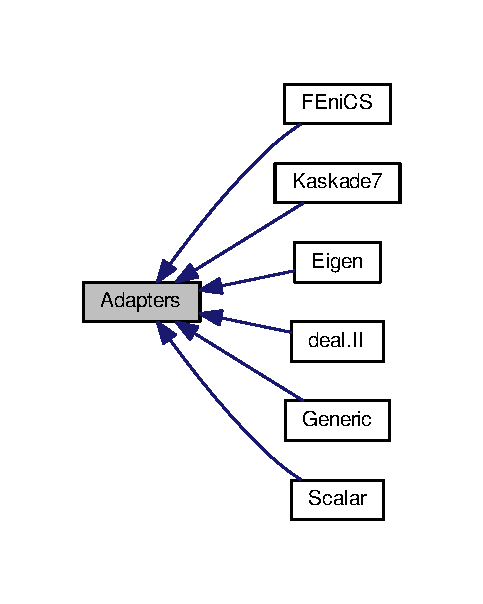
\includegraphics[width=232pt]{group__AdapterGroup}
\end{center}
\end{figure}
\subsection*{\-Modules}
\begin{DoxyCompactItemize}
\item 
\hyperlink{group__FenicsGroup}{\-F\-Eni\-C\-S}
\begin{DoxyCompactList}\small\item\em \-Vector spaces, functionals and operators for \href{http://www.fenicsproject.org}{\tt \-F\-Eni\-C\-S}. \end{DoxyCompactList}\item 
\hyperlink{group__KaskadeGroup}{\-Kaskade7}
\begin{DoxyCompactList}\small\item\em \-Vector spaces, functionals and operators for \href{http://www.zib.de/projects/kaskade7-finite-element-toolbox}{\tt \-Kaskade7}. \end{DoxyCompactList}\item 
\hyperlink{group__EigenGroup}{\-Eigen}
\begin{DoxyCompactList}\small\item\em \-Vector spaces, functionals and operators for \href{http://eigen.tuxfamily.org}{\tt \-Eigen}. \end{DoxyCompactList}\item 
\hyperlink{group__GenericGroup}{\-Generic}
\begin{DoxyCompactList}\small\item\em \hyperlink{namespaceSpacy_1_1Generic}{\-Generic} implementations for vector spaces to simplify the implementation of adapters. \end{DoxyCompactList}\item 
\hyperlink{group__ScalarGroup}{\-Scalar}
\begin{DoxyCompactList}\small\item\em \-Everything required for one-\/dimensional problems. \end{DoxyCompactList}\end{DoxyCompactItemize}


\subsection{\-Detailed \-Description}
\-Adapters to third-\/party libraries. \-M\-O\-D\-U\-L\-E\-S 
\hypertarget{group__FenicsGroup}{\section{F\-Eni\-C\-S}
\label{group__FenicsGroup}\index{F\-Eni\-C\-S@{F\-Eni\-C\-S}}
}


Vector spaces, functionals and operators for \href{http://www.fenicsproject.org}{\tt F\-Eni\-C\-S}.  


Collaboration diagram for F\-Eni\-C\-S\-:
\nopagebreak
\begin{figure}[H]
\begin{center}
\leavevmode
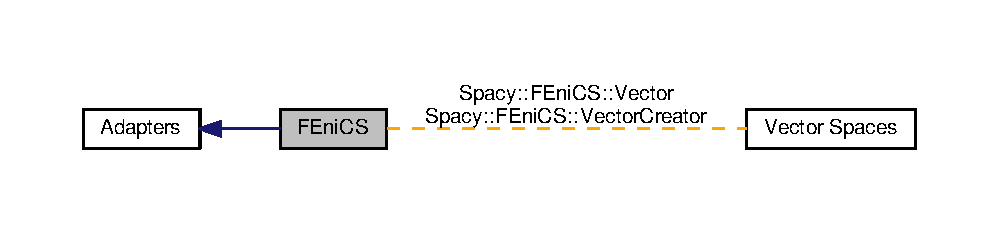
\includegraphics[width=350pt]{group__FenicsGroup}
\end{center}
\end{figure}
\subsection*{Namespaces}
\begin{DoxyCompactItemize}
\item 
\hyperlink{namespaceSpacy_1_1FEniCS}{Spacy\-::\-F\-Eni\-C\-S}
\begin{DoxyCompactList}\small\item\em Contains vector spaces, functionals and operators for \href{www.fenicsproject.org}{\tt F\-Eni\-C\-S}. \end{DoxyCompactList}\end{DoxyCompactItemize}
\subsection*{Classes}
\begin{DoxyCompactItemize}
\item 
class \hyperlink{classSpacy_1_1FEniCS_1_1l2Product}{Spacy\-::\-F\-Eni\-C\-S\-::l2\-Product}
\begin{DoxyCompactList}\small\item\em l2-\/product $(x,y) = \sum_i x_i y_i $ for F\-Eni\-C\-S. \end{DoxyCompactList}\item 
class \hyperlink{classSpacy_1_1FEniCS_1_1LinearOperator}{Spacy\-::\-F\-Eni\-C\-S\-::\-Linear\-Operator}
\begin{DoxyCompactList}\small\item\em Linear operator interface for operators in F\-Eni\-C\-S. \end{DoxyCompactList}\item 
class \hyperlink{classSpacy_1_1FEniCS_1_1LUSolver}{Spacy\-::\-F\-Eni\-C\-S\-::\-L\-U\-Solver}
\begin{DoxyCompactList}\small\item\em L\-U solver for F\-Eni\-C\-S. \end{DoxyCompactList}\item 
class \hyperlink{classSpacy_1_1FEniCS_1_1TransposedLUSolver}{Spacy\-::\-F\-Eni\-C\-S\-::\-Transposed\-L\-U\-Solver}
\begin{DoxyCompactList}\small\item\em Transposed L\-U solver for F\-Eni\-C\-S. \end{DoxyCompactList}\item 
class \hyperlink{classSpacy_1_1FEniCS_1_1Vector}{Spacy\-::\-F\-Eni\-C\-S\-::\-Vector}
\begin{DoxyCompactList}\small\item\em Vector implementation for F\-Eni\-C\-S (single space). \end{DoxyCompactList}\item 
class \hyperlink{classSpacy_1_1FEniCS_1_1VectorCreator}{Spacy\-::\-F\-Eni\-C\-S\-::\-Vector\-Creator}
\begin{DoxyCompactList}\small\item\em Creator for vector space elements for F\-Eni\-C\-S. \end{DoxyCompactList}\end{DoxyCompactItemize}
\subsection*{Functions}
\begin{DoxyCompactItemize}
\item 
void \hyperlink{group__FenicsGroup_gab3d4c7c1e91a50e4e816598258b6edce}{Spacy\-::\-F\-Eni\-C\-S\-::copy\-Coefficients} (const dolfin\-::\-Form \&F, dolfin\-::\-Form \&G)
\begin{DoxyCompactList}\small\item\em Copy coefficients of F to G. \end{DoxyCompactList}\item 
void \hyperlink{group__FenicsGroup_ga7f43f0c660d0646adb031b453c536bb0}{Spacy\-::\-F\-Eni\-C\-S\-::copy} (const \-::\hyperlink{classSpacy_1_1Vector}{Spacy\-::\-Vector} \&x, dolfin\-::\-Generic\-Vector \&y)
\begin{DoxyCompactList}\small\item\em Copy from \hyperlink{classSpacy_1_1Vector}{Spacy\-::\-Vector} to dolfin\-::\-Generic\-Vector. \end{DoxyCompactList}\item 
void \hyperlink{group__FenicsGroup_ga28fb1ebae29e07ec0256bb2331599aa7}{Spacy\-::\-F\-Eni\-C\-S\-::copy} (const \-::\hyperlink{classSpacy_1_1Vector}{Spacy\-::\-Vector} \&x, dolfin\-::\-Function \&y)
\begin{DoxyCompactList}\small\item\em Copy from \hyperlink{classSpacy_1_1Vector}{Spacy\-::\-Vector} to dolfin\-::\-Function. \end{DoxyCompactList}\item 
void \hyperlink{group__FenicsGroup_ga61c5e45dbb789c155fbf86f8ec288f17}{Spacy\-::\-F\-Eni\-C\-S\-::copy} (const dolfin\-::\-Generic\-Vector \&y,\-::\hyperlink{classSpacy_1_1Vector}{Spacy\-::\-Vector} \&x)
\begin{DoxyCompactList}\small\item\em Copy from dolfin\-::\-Generic\-Vector to \hyperlink{classSpacy_1_1Vector}{Spacy\-::\-Vector}. \end{DoxyCompactList}\item 
Vector\-Space \hyperlink{group__FenicsGroup_ga8b67cb3d0188d2398625595b79e2fa6a}{Spacy\-::\-F\-Eni\-C\-S\-::make\-Hilbert\-Space} (std\-::shared\-\_\-ptr$<$ dolfin\-::\-Function\-Space $>$ space)
\begin{DoxyCompactList}\small\item\em Convenient generation of a single vector space from dolfin\-::\-Function\-Space. \end{DoxyCompactList}\item 
Vector\-Space \hyperlink{group__FenicsGroup_ga135620ce224178541cae896577f438dc}{Spacy\-::\-F\-Eni\-C\-S\-::make\-Hilbert\-Space} (std\-::shared\-\_\-ptr$<$ dolfin\-::\-Function\-Space $>$ space, const std\-::unordered\-\_\-map$<$ std\-::size\-\_\-t, std\-::size\-\_\-t $>$ \&dofmap)
\begin{DoxyCompactList}\small\item\em Convenient generation of a single vector space from dolfin\-::\-Function\-Space. \end{DoxyCompactList}\item 
Vector\-Space \hyperlink{group__FenicsGroup_ga79df66c976cab487d2013de25c17bb39}{Spacy\-::\-F\-Eni\-C\-S\-::make\-Hilbert\-Space} (std\-::shared\-\_\-ptr$<$ dolfin\-::\-Function\-Space $>$ space, const std\-::vector$<$ unsigned $>$ \&primal\-Ids, const std\-::vector$<$ unsigned $>$ \&dual\-Ids=\{\})
\begin{DoxyCompactList}\small\item\em Convenient generation of a product space from dolfin\-::\-Function\-Space. \end{DoxyCompactList}\end{DoxyCompactItemize}


\subsection{Detailed Description}
Vector spaces, functionals and operators for \href{http://www.fenicsproject.org}{\tt F\-Eni\-C\-S}. 

\subsection{Function Documentation}
\hypertarget{group__FenicsGroup_gab3d4c7c1e91a50e4e816598258b6edce}{\index{F\-Eni\-C\-S@{F\-Eni\-C\-S}!copy\-Coefficients@{copy\-Coefficients}}
\index{copy\-Coefficients@{copy\-Coefficients}!FEniCS@{F\-Eni\-C\-S}}
\subsubsection[{copy\-Coefficients}]{\setlength{\rightskip}{0pt plus 5cm}void Spacy\-::\-F\-Eni\-C\-S\-::copy\-Coefficients (
\begin{DoxyParamCaption}
\item[{const dolfin\-::\-Form \&}]{F, }
\item[{dolfin\-::\-Form \&}]{G}
\end{DoxyParamCaption}
)}}\label{group__FenicsGroup_gab3d4c7c1e91a50e4e816598258b6edce}


Copy coefficients of F to G. 

Whatever the copy-\/constructor for dolfin forms does it does not copy. So if you want to copy these do the following. Create A new form from the function spaces stored in G. Then copy the coefficients with this function. \hypertarget{group__FenicsGroup_ga7f43f0c660d0646adb031b453c536bb0}{\index{F\-Eni\-C\-S@{F\-Eni\-C\-S}!copy@{copy}}
\index{copy@{copy}!FEniCS@{F\-Eni\-C\-S}}
\subsubsection[{copy}]{\setlength{\rightskip}{0pt plus 5cm}void Spacy\-::\-F\-Eni\-C\-S\-::copy (
\begin{DoxyParamCaption}
\item[{const \-::{\bf Spacy\-::\-Vector} \&}]{x, }
\item[{dolfin\-::\-Generic\-Vector \&}]{y}
\end{DoxyParamCaption}
)}}\label{group__FenicsGroup_ga7f43f0c660d0646adb031b453c536bb0}


Copy from \hyperlink{classSpacy_1_1Vector}{Spacy\-::\-Vector} to dolfin\-::\-Generic\-Vector. 

Does consider product space structures. \begin{DoxySeeAlso}{See Also}
\hyperlink{namespaceSpacy_1_1ProductSpace}{Product\-Space} 
\end{DoxySeeAlso}
\hypertarget{group__FenicsGroup_ga28fb1ebae29e07ec0256bb2331599aa7}{\index{F\-Eni\-C\-S@{F\-Eni\-C\-S}!copy@{copy}}
\index{copy@{copy}!FEniCS@{F\-Eni\-C\-S}}
\subsubsection[{copy}]{\setlength{\rightskip}{0pt plus 5cm}void Spacy\-::\-F\-Eni\-C\-S\-::copy (
\begin{DoxyParamCaption}
\item[{const \-::{\bf Spacy\-::\-Vector} \&}]{x, }
\item[{dolfin\-::\-Function \&}]{y}
\end{DoxyParamCaption}
)}}\label{group__FenicsGroup_ga28fb1ebae29e07ec0256bb2331599aa7}


Copy from \hyperlink{classSpacy_1_1Vector}{Spacy\-::\-Vector} to dolfin\-::\-Function. 

Does consider product space structures. \begin{DoxySeeAlso}{See Also}
\hyperlink{namespaceSpacy_1_1ProductSpace}{Product\-Space} 
\end{DoxySeeAlso}
\hypertarget{group__FenicsGroup_ga61c5e45dbb789c155fbf86f8ec288f17}{\index{F\-Eni\-C\-S@{F\-Eni\-C\-S}!copy@{copy}}
\index{copy@{copy}!FEniCS@{F\-Eni\-C\-S}}
\subsubsection[{copy}]{\setlength{\rightskip}{0pt plus 5cm}void Spacy\-::\-F\-Eni\-C\-S\-::copy (
\begin{DoxyParamCaption}
\item[{const dolfin\-::\-Generic\-Vector \&}]{y, }
\item[{\-::{\bf Spacy\-::\-Vector} \&}]{x}
\end{DoxyParamCaption}
)}}\label{group__FenicsGroup_ga61c5e45dbb789c155fbf86f8ec288f17}


Copy from dolfin\-::\-Generic\-Vector to \hyperlink{classSpacy_1_1Vector}{Spacy\-::\-Vector}. 

Does consider product space structures. \begin{DoxySeeAlso}{See Also}
\hyperlink{group__ProductSpaceGroup}{Product Space} 
\end{DoxySeeAlso}
\hypertarget{group__FenicsGroup_ga8b67cb3d0188d2398625595b79e2fa6a}{\index{F\-Eni\-C\-S@{F\-Eni\-C\-S}!make\-Hilbert\-Space@{make\-Hilbert\-Space}}
\index{make\-Hilbert\-Space@{make\-Hilbert\-Space}!FEniCS@{F\-Eni\-C\-S}}
\subsubsection[{make\-Hilbert\-Space}]{\setlength{\rightskip}{0pt plus 5cm}Vector\-Space Spacy\-::\-F\-Eni\-C\-S\-::make\-Hilbert\-Space (
\begin{DoxyParamCaption}
\item[{std\-::shared\-\_\-ptr$<$ dolfin\-::\-Function\-Space $>$}]{space}
\end{DoxyParamCaption}
)}}\label{group__FenicsGroup_ga8b67cb3d0188d2398625595b79e2fa6a}


Convenient generation of a single vector space from dolfin\-::\-Function\-Space. 


\begin{DoxyParams}{Parameters}
{\em space} & single dolfin\-::\-Function\-Space (no product space) \\
\hline
\end{DoxyParams}
\begin{DoxyReturn}{Returns}
\hyperlink{namespaceSpacy_a927756dd42df3e79c302df1f8f635b65}{\-:\-:Spacy\-:\-:make\-Hilbert\-Space( Vector\-Creator\{space\} , l2\-Product\{\} )} 
\end{DoxyReturn}
\hypertarget{group__FenicsGroup_ga135620ce224178541cae896577f438dc}{\index{F\-Eni\-C\-S@{F\-Eni\-C\-S}!make\-Hilbert\-Space@{make\-Hilbert\-Space}}
\index{make\-Hilbert\-Space@{make\-Hilbert\-Space}!FEniCS@{F\-Eni\-C\-S}}
\subsubsection[{make\-Hilbert\-Space}]{\setlength{\rightskip}{0pt plus 5cm}Vector\-Space Spacy\-::\-F\-Eni\-C\-S\-::make\-Hilbert\-Space (
\begin{DoxyParamCaption}
\item[{std\-::shared\-\_\-ptr$<$ dolfin\-::\-Function\-Space $>$}]{space, }
\item[{const std\-::unordered\-\_\-map$<$ std\-::size\-\_\-t, std\-::size\-\_\-t $>$ \&}]{dofmap}
\end{DoxyParamCaption}
)}}\label{group__FenicsGroup_ga135620ce224178541cae896577f438dc}


Convenient generation of a single vector space from dolfin\-::\-Function\-Space. 


\begin{DoxyParams}{Parameters}
{\em space} & single dolfin\-::\-Function\-Space (no product space) \\
\hline
{\em dofmap} & map relating global ids of a product space to local ids in this single space \\
\hline
\end{DoxyParams}
\begin{DoxyReturn}{Returns}
\hyperlink{namespaceSpacy_a927756dd42df3e79c302df1f8f635b65}{\-:\-:Spacy\-:\-:make\-Hilbert\-Space( Vector\-Creator\{space,dofmap\} , l2\-Product\{\} )} 
\end{DoxyReturn}
\hypertarget{group__FenicsGroup_ga79df66c976cab487d2013de25c17bb39}{\index{F\-Eni\-C\-S@{F\-Eni\-C\-S}!make\-Hilbert\-Space@{make\-Hilbert\-Space}}
\index{make\-Hilbert\-Space@{make\-Hilbert\-Space}!FEniCS@{F\-Eni\-C\-S}}
\subsubsection[{make\-Hilbert\-Space}]{\setlength{\rightskip}{0pt plus 5cm}Vector\-Space Spacy\-::\-F\-Eni\-C\-S\-::make\-Hilbert\-Space (
\begin{DoxyParamCaption}
\item[{std\-::shared\-\_\-ptr$<$ dolfin\-::\-Function\-Space $>$}]{space, }
\item[{const std\-::vector$<$ unsigned $>$ \&}]{primal\-Ids, }
\item[{const std\-::vector$<$ unsigned $>$ \&}]{dual\-Ids = {\ttfamily \{\}}}
\end{DoxyParamCaption}
)}}\label{group__FenicsGroup_ga79df66c976cab487d2013de25c17bb39}


Convenient generation of a product space from dolfin\-::\-Function\-Space. 


\begin{DoxyParams}{Parameters}
{\em space} & single dolfin\-::\-Function\-Space (product space) \\
\hline
{\em primal\-Ids} & indices of spaces associated with primal variables \\
\hline
{\em dual\-Ids} & indices of spaces associated with dual variables \\
\hline
\end{DoxyParams}
\begin{DoxyReturn}{Returns}
primal-\/dual product space 
\end{DoxyReturn}

\hypertarget{group__KaskadeGroup}{\section{Kaskade7}
\label{group__KaskadeGroup}\index{Kaskade7@{Kaskade7}}
}


Vector spaces, functionals and operators for \href{http://www.zib.de/projects/kaskade7-finite-element-toolbox}{\tt Kaskade7}.  


Collaboration diagram for Kaskade7\-:
\nopagebreak
\begin{figure}[H]
\begin{center}
\leavevmode
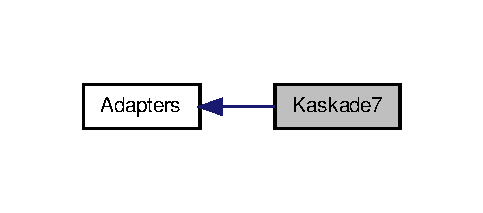
\includegraphics[width=232pt]{group__KaskadeGroup}
\end{center}
\end{figure}
\subsection*{Namespaces}
\begin{DoxyCompactItemize}
\item 
\hyperlink{namespaceSpacy_1_1Kaskade}{Spacy\-::\-Kaskade}
\begin{DoxyCompactList}\small\item\em Contains vector spaces, functionals and operators for \href{http://www.zib.de/projects/kaskade7-finite-element-toolbox}{\tt Kaskade7}. \end{DoxyCompactList}\end{DoxyCompactItemize}
\subsection*{Classes}
\begin{DoxyCompactItemize}
\item 
class \hyperlink{classSpacy_1_1Kaskade_1_1DirectSolver}{Spacy\-::\-Kaskade\-::\-Direct\-Solver$<$ Kaskade\-Operator, Ansatz\-Variable\-Description, Test\-Variable\-Description $>$}
\begin{DoxyCompactList}\small\item\em Direct solver interface for Kaskade 7. \end{DoxyCompactList}\item 
class \hyperlink{classSpacy_1_1Kaskade_1_1l2Product}{Spacy\-::\-Kaskade\-::l2\-Product$<$ Description $>$}
\begin{DoxyCompactList}\small\item\em \hyperlink{namespaceSpacy_1_1Generic}{Generic} l2 scalar product for Kaskade7. Based on the implementation of the dual pairing. \end{DoxyCompactList}\item 
class \hyperlink{classSpacy_1_1Kaskade_1_1Lagrange_1_1CGCreator}{Spacy\-::\-Kaskade\-::\-Lagrange\-::\-C\-G\-Creator$<$ Functional\-Definition, state\-Id, control\-Id, adjoint\-Id $>$}
\begin{DoxyCompactList}\small\item\em Creator for conjugate gradient solver for optimal control problems with a \hyperlink{classSpacy_1_1CG_1_1TriangularStateConstraintPreconditioner}{C\-G\-::\-Triangular\-State\-Constraint\-Preconditioner}. \end{DoxyCompactList}\item 
class \hyperlink{classSpacy_1_1Kaskade_1_1Operator}{Spacy\-::\-Kaskade\-::\-Operator$<$ Operator\-Definition $>$}
\begin{DoxyCompactList}\small\item\em Operator interface for Kaskade 7. Models an operator $A:X\rightarrow Y$. \end{DoxyCompactList}\item 
class \hyperlink{classSpacy_1_1Kaskade_1_1Vector}{Spacy\-::\-Kaskade\-::\-Vector$<$ Description $>$}
\begin{DoxyCompactList}\small\item\em Coefficient vector implementation for Kaskade 7 (single space). \end{DoxyCompactList}\item 
class \hyperlink{classSpacy_1_1KaskadeParabolic_1_1OCP_1_1DirectBlockPreconditioner}{Spacy\-::\-Kaskade\-Parabolic\-::\-O\-C\-P\-::\-Direct\-Block\-Preconditioner$<$ Functional\-Definition $>$}
\begin{DoxyCompactList}\small\item\em A constraint preconditioner for optimal control problems that uses a direct solver. \end{DoxyCompactList}\end{DoxyCompactItemize}
\subsection*{Functions}
\begin{DoxyCompactItemize}
\item 
{\footnotesize template$<$class Operator\-Definition $>$ }\\auto \hyperlink{group__KaskadeGroup_ga0e8d7d2c51e429e22561ef813fc97589}{Spacy\-::\-Kaskade\-::make\-Operator} (const Operator\-Definition \&f, const Vector\-Space \&domain, const Vector\-Space \&range)
\begin{DoxyCompactList}\small\item\em Convenient generation of a differentiable operator $A: X\rightarrow Y$ from Kaskade 7. \end{DoxyCompactList}\item 
{\footnotesize template$<$class Operator\-Definition $>$ }\\auto \hyperlink{group__KaskadeGroup_ga3afbd00437ea7bdb406f3d9a1f375522}{Spacy\-::\-Kaskade\-::make\-Operator} (const Operator\-Definition \&f, const Vector\-Space \&domain)
\begin{DoxyCompactList}\small\item\em Convenient generation of a differentiable operator $A: X\rightarrow X^*$ from Kaskade 7. \end{DoxyCompactList}\end{DoxyCompactItemize}


\subsection{Detailed Description}
Vector spaces, functionals and operators for \href{http://www.zib.de/projects/kaskade7-finite-element-toolbox}{\tt Kaskade7}. 

\subsection{Function Documentation}
\hypertarget{group__KaskadeGroup_ga0e8d7d2c51e429e22561ef813fc97589}{\index{Kaskade7@{Kaskade7}!make\-Operator@{make\-Operator}}
\index{make\-Operator@{make\-Operator}!Kaskade7@{Kaskade7}}
\subsubsection[{make\-Operator}]{\setlength{\rightskip}{0pt plus 5cm}template$<$class Operator\-Definition $>$ auto Spacy\-::\-Kaskade\-::make\-Operator (
\begin{DoxyParamCaption}
\item[{const Operator\-Definition \&}]{f, }
\item[{const Vector\-Space \&}]{domain, }
\item[{const Vector\-Space \&}]{range}
\end{DoxyParamCaption}
)}}\label{group__KaskadeGroup_ga0e8d7d2c51e429e22561ef813fc97589}


Convenient generation of a differentiable operator $A: X\rightarrow Y$ from Kaskade 7. 


\begin{DoxyParams}{Parameters}
{\em f} & operator definition from Kaskade 7 \\
\hline
{\em domain} & domain space $X$ \\
\hline
{\em range} & range space $Y$ \\
\hline
\end{DoxyParams}
\begin{DoxyReturn}{Returns}
\hyperlink{classSpacy_1_1Kaskade_1_1Operator}{\-:\-:Spacy\-:\-:Kaskade\-:\-:Operator$<$Operator\-Definition$>$( A , domain , range )} 
\end{DoxyReturn}
\hypertarget{group__KaskadeGroup_ga3afbd00437ea7bdb406f3d9a1f375522}{\index{Kaskade7@{Kaskade7}!make\-Operator@{make\-Operator}}
\index{make\-Operator@{make\-Operator}!Kaskade7@{Kaskade7}}
\subsubsection[{make\-Operator}]{\setlength{\rightskip}{0pt plus 5cm}template$<$class Operator\-Definition $>$ auto Spacy\-::\-Kaskade\-::make\-Operator (
\begin{DoxyParamCaption}
\item[{const Operator\-Definition \&}]{f, }
\item[{const Vector\-Space \&}]{domain}
\end{DoxyParamCaption}
)}}\label{group__KaskadeGroup_ga3afbd00437ea7bdb406f3d9a1f375522}


Convenient generation of a differentiable operator $A: X\rightarrow X^*$ from Kaskade 7. 


\begin{DoxyParams}{Parameters}
{\em f} & operator definition from Kaskade 7 \\
\hline
{\em domain} & domain space $X$ \\
\hline
\end{DoxyParams}
\begin{DoxyReturn}{Returns}
\hyperlink{classSpacy_1_1Kaskade_1_1Operator}{\-:\-:Spacy\-:\-:Kaskade\-:\-:Operator$<$Operator\-Definition$>$( A , domain , range )} 
\end{DoxyReturn}

\hypertarget{group__EigenGroup}{}\section{Eigen}
\label{group__EigenGroup}\index{Eigen@{Eigen}}


Vector spaces, functionals and operators for \href{http://eigen.tuxfamily.org}{\tt Eigen}.  


Collaboration diagram for Eigen\+:
\nopagebreak
\begin{figure}[H]
\begin{center}
\leavevmode
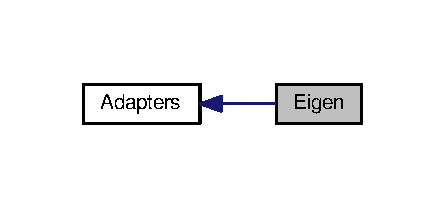
\includegraphics[width=213pt]{group__EigenGroup}
\end{center}
\end{figure}
\subsection*{Classes}
\begin{DoxyCompactItemize}
\item 
class \hyperlink{classSpacy_1_1Rn_1_1C1Operator}{Spacy\+::\+Rn\+::\+C1\+Operator}
\begin{DoxyCompactList}\small\item\em A differential operator $A:X\rightarrow Y$ for finite-\/dimensional problems, based on the Eigen library. \end{DoxyCompactList}\item 
class \hyperlink{classSpacy_1_1Rn_1_1LinearOperator}{Spacy\+::\+Rn\+::\+Linear\+Operator}
\begin{DoxyCompactList}\small\item\em A linear operator $A:X\rightarrow Y$ for finite-\/dimensional problems, based on the Eigen library. \end{DoxyCompactList}\item 
struct \hyperlink{structSpacy_1_1Rn_1_1LinearOperatorCreator}{Spacy\+::\+Rn\+::\+Linear\+Operator\+Creator}
\begin{DoxyCompactList}\small\item\em Vector\+Creator for linear operators $X\rightarrow Y$, based on the Eigen library. \end{DoxyCompactList}\item 
class \hyperlink{classSpacy_1_1Rn_1_1LinearSolver}{Spacy\+::\+Rn\+::\+Linear\+Solver}
\begin{DoxyCompactList}\small\item\em Linear solver for Eigen matrices. \end{DoxyCompactList}\end{DoxyCompactItemize}
\subsection*{Typedefs}
\begin{DoxyCompactItemize}
\item 
using \hyperlink{group__EigenGroup_gaf2be4f79056513f7e3e35f7afdc794ee}{Spacy\+::\+Rn\+::\+Euclidean\+Scalar\+Product} = Generic\+::\+Euclidean\+Scalar\+Product\hypertarget{group__EigenGroup_gaf2be4f79056513f7e3e35f7afdc794ee}{}\label{group__EigenGroup_gaf2be4f79056513f7e3e35f7afdc794ee}

\begin{DoxyCompactList}\small\item\em Euclidean scalar product for Rn, based on the Eigen library. \end{DoxyCompactList}\end{DoxyCompactItemize}


\subsection{Detailed Description}
Vector spaces, functionals and operators for \href{http://eigen.tuxfamily.org}{\tt Eigen}. 


\hypertarget{group__GenericGroup}{\section{Generic}
\label{group__GenericGroup}\index{Generic@{Generic}}
}


Generic implementations for vector spaces to simplify the implementation of adapters.  


Collaboration diagram for Generic\-:
\nopagebreak
\begin{figure}[H]
\begin{center}
\leavevmode
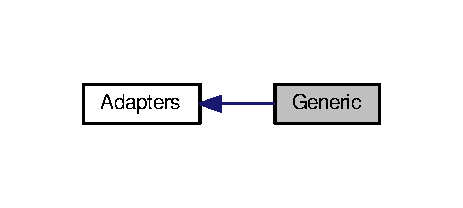
\includegraphics[width=222pt]{group__GenericGroup}
\end{center}
\end{figure}
\subsection*{Classes}
\begin{DoxyCompactItemize}
\item 
class \hyperlink{classSpacy_1_1Generic_1_1EuclideanScalarProduct}{Spacy\-::\-Generic\-::\-Euclidean\-Scalar\-Product}
\begin{DoxyCompactList}\small\item\em \hyperlink{namespaceSpacy_1_1Generic}{Generic} euclidean scalar product, based on the dual pairing in hilbert spaces. \end{DoxyCompactList}\item 
class \hyperlink{classSpacy_1_1Generic_1_1Vector}{Spacy\-::\-Generic\-::\-Vector$<$ Vector\-Impl $>$}
\begin{DoxyCompactList}\small\item\em \hyperlink{namespaceSpacy_1_1Generic}{Generic} vector implementation for Rn. \end{DoxyCompactList}\item 
class \hyperlink{classSpacy_1_1Generic_1_1VectorCreator}{Spacy\-::\-Generic\-::\-Vector\-Creator$<$ Vector\-Impl $>$}
\begin{DoxyCompactList}\small\item\em \hyperlink{namespaceSpacy_1_1Generic}{Generic} vector creator implementation. \end{DoxyCompactList}\end{DoxyCompactItemize}


\subsection{Detailed Description}
Generic implementations for vector spaces to simplify the implementation of adapters. 
\hypertarget{group__ScalarGroup}{\section{\-Scalar}
\label{group__ScalarGroup}\index{\-Scalar@{\-Scalar}}
}


\-Operators, functionals and solvers for scalar problems.  


\-Collaboration diagram for \-Scalar\-:
\nopagebreak
\begin{figure}[H]
\begin{center}
\leavevmode
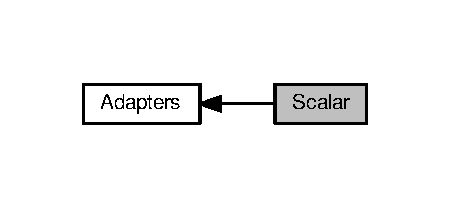
\includegraphics[width=216pt]{group__ScalarGroup}
\end{center}
\end{figure}
\-Operators, functionals and solvers for scalar problems. 
\hypertarget{group__VectorSpaceGroup}{\section{Vector Spaces}
\label{group__VectorSpaceGroup}\index{Vector Spaces@{Vector Spaces}}
}


Collection of available vector spaces.  


Collaboration diagram for Vector Spaces\-:
\nopagebreak
\begin{figure}[H]
\begin{center}
\leavevmode
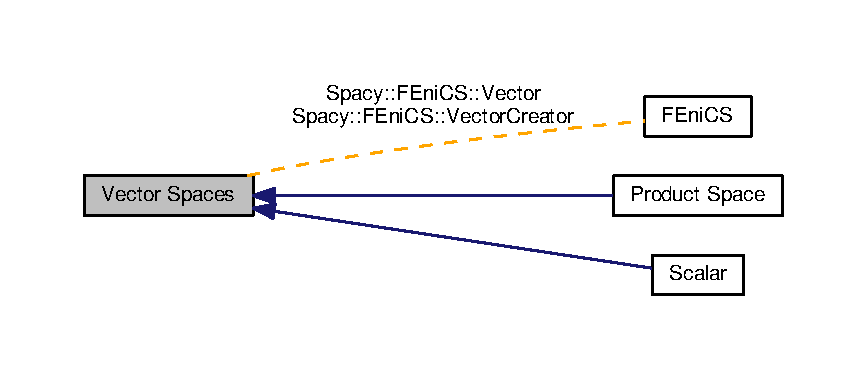
\includegraphics[width=350pt]{group__VectorSpaceGroup}
\end{center}
\end{figure}
\subsection*{Modules}
\begin{DoxyCompactItemize}
\item 
\hyperlink{group__ScalarGroup}{Scalar}
\begin{DoxyCompactList}\small\item\em Everything required for one-\/dimensional problems. \end{DoxyCompactList}\item 
\hyperlink{group__ProductSpaceGroup}{Product Space}
\begin{DoxyCompactList}\small\item\em A product space that supports distinction between primal and dual variables. \end{DoxyCompactList}\end{DoxyCompactItemize}
\subsection*{Classes}
\begin{DoxyCompactItemize}
\item 
class \hyperlink{classSpacy_1_1FEniCS_1_1Vector}{Spacy\-::\-F\-Eni\-C\-S\-::\-Vector}
\begin{DoxyCompactList}\small\item\em Vector implementation for F\-Eni\-C\-S (single space). \end{DoxyCompactList}\item 
class \hyperlink{classSpacy_1_1FEniCS_1_1VectorCreator}{Spacy\-::\-F\-Eni\-C\-S\-::\-Vector\-Creator}
\begin{DoxyCompactList}\small\item\em Creator for vector space elements for F\-Eni\-C\-S. \end{DoxyCompactList}\end{DoxyCompactItemize}
\subsection*{Typedefs}
\begin{DoxyCompactItemize}
\item 
using \hyperlink{group__VectorSpaceGroup_ga65d64ee5f22f492639d0f950aa931071}{Spacy\-::deal\-I\-I\-::\-Vector} = Generic\-::\-Vector$<$ dealii\-::\-Vector$<$ double $>$ $>$
\begin{DoxyCompactList}\small\item\em Vector adapter for deal.\-I\-I \end{DoxyCompactList}\item 
using \hyperlink{group__VectorSpaceGroup_gafda42fd5aa3f7597a42b9831bf4dfd07}{Spacy\-::\-Rn\-::\-Vector} = Generic\-::\-Vector$<$ \-::Eigen\-::\-Vector\-Xd $>$
\begin{DoxyCompactList}\small\item\em Vector for Rn, based on the Eigen library. \end{DoxyCompactList}\end{DoxyCompactItemize}
\subsection*{Functions}
\begin{DoxyCompactItemize}
\item 
{\footnotesize template$<$class... Args, class  = std\-::enable\-\_\-if\-\_\-t$<$std\-::is\-\_\-constructible$<$\-Description,\-Args...$>$\-::value$>$$>$ }\\\hyperlink{group__VectorSpaceGroup_ga89de372343310640870077e6167df3f4}{Spacy\-::\-Kaskade\-::\-Vector\-Creator$<$ Description $>$\-::\-Vector\-Creator} (Args \&\&...args)
\begin{DoxyCompactList}\small\item\em Create from Kaskade 7 function space. \end{DoxyCompactList}\item 
{\footnotesize template$<$class Description $>$ }\\auto \hyperlink{group__VectorSpaceGroup_ga04d45446864bbf87770d02eade7b64cf}{Spacy\-::\-Kaskade\-::make\-Hilbert\-Space} (const Description \&description)
\begin{DoxyCompactList}\small\item\em Create single space with hilbert space structure for Kaskade 7. \end{DoxyCompactList}\item 
{\footnotesize template$<$class Description $>$ }\\auto \hyperlink{group__VectorSpaceGroup_ga221db25c41371a2a823a6b569d735ef6}{Spacy\-::\-Kaskade\-::make\-Hilbert\-Space} (const Description \&description, const std\-::vector$<$ unsigned $>$ \&primal\-Ids, const std\-::vector$<$ unsigned $>$ \&dual\-Ids=\{\})
\begin{DoxyCompactList}\small\item\em Create product space with hilbert space structure for Kaskade 7. \end{DoxyCompactList}\end{DoxyCompactItemize}


\subsection{Detailed Description}
Collection of available vector spaces. Contains models for one-\/dimensional and product spaces as well as vector spaces for F\-Enics and Kaskade 7. 

\subsection{Typedef Documentation}
\hypertarget{group__VectorSpaceGroup_ga65d64ee5f22f492639d0f950aa931071}{\index{Vector Spaces@{Vector Spaces}!Vector@{Vector}}
\index{Vector@{Vector}!Vector Spaces@{Vector Spaces}}
\subsubsection[{Vector}]{\setlength{\rightskip}{0pt plus 5cm}using {\bf Spacy\-::deal\-I\-I\-::\-Vector} = typedef Generic\-::\-Vector$<$ dealii\-::\-Vector$<$double$>$ $>$}}\label{group__VectorSpaceGroup_ga65d64ee5f22f492639d0f950aa931071}


Vector adapter for deal.\-I\-I 

, \hypertarget{group__VectorSpaceGroup_gafda42fd5aa3f7597a42b9831bf4dfd07}{\index{Vector Spaces@{Vector Spaces}!Vector@{Vector}}
\index{Vector@{Vector}!Vector Spaces@{Vector Spaces}}
\subsubsection[{Vector}]{\setlength{\rightskip}{0pt plus 5cm}using {\bf Spacy\-::\-Rn\-::\-Vector} = typedef Generic\-::\-Vector$<$ \-::Eigen\-::\-Vector\-Xd $>$}}\label{group__VectorSpaceGroup_gafda42fd5aa3f7597a42b9831bf4dfd07}


Vector for Rn, based on the Eigen library. 

, 

\subsection{Function Documentation}
\hypertarget{group__VectorSpaceGroup_ga89de372343310640870077e6167df3f4}{\index{Vector Spaces@{Vector Spaces}!Vector\-Creator@{Vector\-Creator}}
\index{Vector\-Creator@{Vector\-Creator}!Vector Spaces@{Vector Spaces}}
\subsubsection[{Vector\-Creator}]{\setlength{\rightskip}{0pt plus 5cm}template$<$class Description $>$ template$<$class... Args, class  = std\-::enable\-\_\-if\-\_\-t$<$std\-::is\-\_\-constructible$<$\-Description,\-Args...$>$\-::value$>$$>$ {\bf Spacy\-::\-Kaskade\-::\-Vector\-Creator}$<$ Description $>$\-::Vector\-Creator (
\begin{DoxyParamCaption}
\item[{Args \&\&...}]{args}
\end{DoxyParamCaption}
)\hspace{0.3cm}{\ttfamily [inline]}}}\label{group__VectorSpaceGroup_ga89de372343310640870077e6167df3f4}


Create from Kaskade 7 function space. 


\begin{DoxyParams}{Parameters}
{\em space} & single Kaskade 7 function space (no product space) \\
\hline
\end{DoxyParams}
\hypertarget{group__VectorSpaceGroup_ga04d45446864bbf87770d02eade7b64cf}{\index{Vector Spaces@{Vector Spaces}!make\-Hilbert\-Space@{make\-Hilbert\-Space}}
\index{make\-Hilbert\-Space@{make\-Hilbert\-Space}!Vector Spaces@{Vector Spaces}}
\subsubsection[{make\-Hilbert\-Space}]{\setlength{\rightskip}{0pt plus 5cm}template$<$class Description $>$ auto Spacy\-::\-Kaskade\-::make\-Hilbert\-Space (
\begin{DoxyParamCaption}
\item[{const Description \&}]{description}
\end{DoxyParamCaption}
)}}\label{group__VectorSpaceGroup_ga04d45446864bbf87770d02eade7b64cf}


Create single space with hilbert space structure for Kaskade 7. 


\begin{DoxyParams}{Parameters}
{\em space} & single Kaskade 7 function space (no product space) \\
\hline
\end{DoxyParams}
\hypertarget{group__VectorSpaceGroup_ga221db25c41371a2a823a6b569d735ef6}{\index{Vector Spaces@{Vector Spaces}!make\-Hilbert\-Space@{make\-Hilbert\-Space}}
\index{make\-Hilbert\-Space@{make\-Hilbert\-Space}!Vector Spaces@{Vector Spaces}}
\subsubsection[{make\-Hilbert\-Space}]{\setlength{\rightskip}{0pt plus 5cm}template$<$class Description $>$ auto Spacy\-::\-Kaskade\-::make\-Hilbert\-Space (
\begin{DoxyParamCaption}
\item[{const Description \&}]{description, }
\item[{const std\-::vector$<$ unsigned $>$ \&}]{primal\-Ids, }
\item[{const std\-::vector$<$ unsigned $>$ \&}]{dual\-Ids = {\ttfamily \{\}}}
\end{DoxyParamCaption}
)}}\label{group__VectorSpaceGroup_ga221db25c41371a2a823a6b569d735ef6}


Create product space with hilbert space structure for Kaskade 7. 


\begin{DoxyParams}{Parameters}
{\em spaces} & boost fusion forward sequence of const pointers to Kaskade 7 function spaces \\
\hline
{\em primal\-Ids} & ids of primal variables \\
\hline
{\em dual\-Ids} & ids of dual variables \\
\hline
\end{DoxyParams}

\hypertarget{group__RealGroup}{\section{\-Real \-Space}
\label{group__RealGroup}\index{\-Real Space@{\-Real Space}}
}


\-A one dimensional vector space representing the space of real numbers.  


\-Collaboration diagram for \-Real \-Space\-:
\nopagebreak
\begin{figure}[H]
\begin{center}
\leavevmode
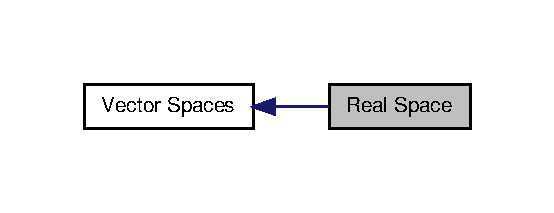
\includegraphics[width=266pt]{group__RealGroup}
\end{center}
\end{figure}
\subsection*{\-Functions}
\begin{DoxyCompactItemize}
\item 
\-Vector\-Space \hyperlink{group__RealGroup_gaa07f743f9874ecff062c511b7126f8b6}{\-Spacy\-::\-Real\-Space\-::make\-Hilbert\-Space} (bool default\-Index=false)
\begin{DoxyCompactList}\small\item\em \-Construct space of real numbers. \end{DoxyCompactList}\end{DoxyCompactItemize}


\subsection{\-Detailed \-Description}
\-A one dimensional vector space representing the space of real numbers. 

\subsection{\-Function \-Documentation}
\hypertarget{group__RealGroup_gaa07f743f9874ecff062c511b7126f8b6}{\index{\-Real Space@{\-Real Space}!make\-Hilbert\-Space@{make\-Hilbert\-Space}}
\index{make\-Hilbert\-Space@{make\-Hilbert\-Space}!Real Space@{\-Real Space}}
\subsubsection[{make\-Hilbert\-Space}]{\setlength{\rightskip}{0pt plus 5cm}\-Vector\-Space {\bf \-Spacy\-::\-Real\-Space\-::make\-Hilbert\-Space} (
\begin{DoxyParamCaption}
\item[{bool}]{default\-Index = {\ttfamily false}}
\end{DoxyParamCaption}
)}}\label{group__RealGroup_gaa07f743f9874ecff062c511b7126f8b6}


\-Construct space of real numbers. 

\begin{DoxyReturn}{\-Returns}
\hyperlink{namespaceSpacy_a927756dd42df3e79c302df1f8f635b65}{\-Spacy\-::make\-Hilbert\-Space()} \char`\"{}\-::\-Spacy\-::make\-Hilbert\-Space( \mbox{[}$\,$\mbox{]}(const Spacy$\ast$ space)\{ return Vector\{$\ast$space\}; \} , Scalar\-Product\{\} )\char`\"{} 
\end{DoxyReturn}

\hypertarget{group__ProductSpaceGroup}{\section{\-Product \-Space}
\label{group__ProductSpaceGroup}\index{\-Product Space@{\-Product Space}}
}


\-A product space that supports distinction between primal and dual variables.  


\-Collaboration diagram for \-Product \-Space\-:
\nopagebreak
\begin{figure}[H]
\begin{center}
\leavevmode
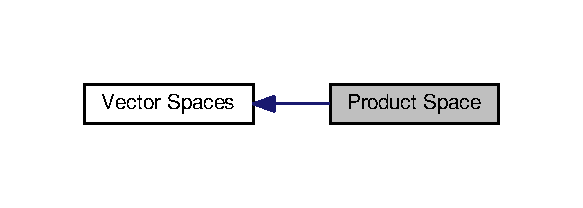
\includegraphics[width=280pt]{group__ProductSpaceGroup}
\end{center}
\end{figure}
\subsection*{\-Classes}
\begin{DoxyCompactItemize}
\item 
class \hyperlink{classSpacy_1_1ProductSpace_1_1Norm}{\-Spacy\-::\-Product\-Space\-::\-Norm}
\begin{DoxyCompactList}\small\item\em \-Canonical norm on product spaces. \end{DoxyCompactList}\item 
class \hyperlink{classSpacy_1_1ProductSpace_1_1ScalarProduct}{\-Spacy\-::\-Product\-Space\-::\-Scalar\-Product}
\begin{DoxyCompactList}\small\item\em \-Canonical scalar product on product spaces. \end{DoxyCompactList}\item 
class \hyperlink{classSpacy_1_1ProductSpace_1_1VectorCreator}{\-Spacy\-::\-Product\-Space\-::\-Vector\-Creator}
\begin{DoxyCompactList}\small\item\em \-Creator for \hyperlink{classSpacy_1_1ProductSpace_1_1Vector}{\-Product\-Space\-::\-Vector}. \end{DoxyCompactList}\end{DoxyCompactItemize}
\subsection*{\-Namespaces}
\begin{DoxyCompactItemize}
\item 
namespace \hyperlink{namespaceSpacy_1_1ProductSpace}{\-Spacy\-::\-Product\-Space}
\begin{DoxyCompactList}\small\item\em \-A product space that supports distinction between primal and dual variables. \end{DoxyCompactList}\end{DoxyCompactItemize}
\subsection*{\-Enumerations}
\begin{DoxyCompactItemize}
\item 
enum \{ {\bfseries \-P\-R\-I\-M\-A\-L} = 0, 
{\bfseries \-D\-U\-A\-L} = 1
 \}
\end{DoxyCompactItemize}
\subsection*{\-Functions}
\begin{DoxyCompactItemize}
\item 
\-::\hyperlink{classSpacy_1_1Vector}{\-Spacy\-::\-Vector} \& \hyperlink{group__ProductSpaceGroup_gaa040ba5c24284687e0df19c99dd688a6}{\-Spacy\-::primal\-Component} (\-::\hyperlink{classSpacy_1_1Vector}{\-Spacy\-::\-Vector} \&v)
\item 
const \-::\hyperlink{classSpacy_1_1Vector}{\-Spacy\-::\-Vector} \& \hyperlink{group__ProductSpaceGroup_ga88c5bcc74072f75c63ab7d9448f80a7e}{\-Spacy\-::primal\-Component} (const \-::\hyperlink{classSpacy_1_1Vector}{\-Spacy\-::\-Vector} \&v)
\item 
\-::\hyperlink{classSpacy_1_1Vector}{\-Spacy\-::\-Vector} \& \hyperlink{group__ProductSpaceGroup_gafe51c084e3b03205db94e91309e834f7}{\-Spacy\-::dual\-Component} (\-::\hyperlink{classSpacy_1_1Vector}{\-Spacy\-::\-Vector} \&v)
\item 
const \-::\hyperlink{classSpacy_1_1Vector}{\-Spacy\-::\-Vector} \& \hyperlink{group__ProductSpaceGroup_gabe5978657aab46b1575e2521b336407d}{\-Spacy\-::dual\-Component} (const \-::\hyperlink{classSpacy_1_1Vector}{\-Spacy\-::\-Vector} \&v)
\item 
\-Vector\-Space \hyperlink{group__ProductSpaceGroup_gad4b421dd4563c7d575550ab4d5d3ff0d}{\-Spacy\-::\-Product\-Space\-::make\-Hilbert\-Space} (const std\-::vector$<$ std\-::shared\-\_\-ptr$<$ \-Vector\-Space $>$ $>$ \&spaces)
\begin{DoxyCompactList}\small\item\em \-Create product space. \end{DoxyCompactList}\item 
\-Vector\-Space \hyperlink{group__ProductSpaceGroup_gaee9c55c4b0f0b9d41bb6e1eba80f829f}{\-Spacy\-::\-Product\-Space\-::make\-Hilbert\-Space} (const std\-::vector$<$ std\-::shared\-\_\-ptr$<$ \-Vector\-Space $>$ $>$ \&spaces, const std\-::vector$<$ unsigned $>$ \&global\-Ids)
\begin{DoxyCompactList}\small\item\em \-Create product space. \end{DoxyCompactList}\item 
\-Vector\-Space \hyperlink{group__ProductSpaceGroup_ga5146524c4a6b3cb6f4a47b877cb2f55d}{\-Spacy\-::\-Product\-Space\-::make\-Hilbert\-Space} (const std\-::vector$<$ std\-::shared\-\_\-ptr$<$ \-Vector\-Space $>$ $>$ \&spaces, const std\-::vector$<$ unsigned $>$ \&primal\-Sub\-Space\-Ids, const std\-::vector$<$ unsigned $>$ \&dual\-Sub\-Space\-Ids)
\begin{DoxyCompactList}\small\item\em \-Create primal-\/dual product space. \end{DoxyCompactList}\end{DoxyCompactItemize}


\subsection{\-Detailed \-Description}
\-A product space that supports distinction between primal and dual variables. 

\subsection{\-Function \-Documentation}
\hypertarget{group__ProductSpaceGroup_gaa040ba5c24284687e0df19c99dd688a6}{\index{\-Product Space@{\-Product Space}!primal\-Component@{primal\-Component}}
\index{primal\-Component@{primal\-Component}!Product Space@{\-Product Space}}
\subsubsection[{primal\-Component}]{\setlength{\rightskip}{0pt plus 5cm}\-::{\bf \-Spacy\-::\-Vector}\& {\bf \-Spacy\-::primal\-Component} (
\begin{DoxyParamCaption}
\item[{\-::{\bf \-Spacy\-::\-Vector} \&}]{v}
\end{DoxyParamCaption}
)}}\label{group__ProductSpaceGroup_gaa040ba5c24284687e0df19c99dd688a6}
\begin{DoxyReturn}{\-Returns}
cast\-\_\-ref$<$\-Product\-Space\-::\-Vector$>$(v).component(\-P\-R\-I\-M\-A\-L); 
\end{DoxyReturn}
\hypertarget{group__ProductSpaceGroup_ga88c5bcc74072f75c63ab7d9448f80a7e}{\index{\-Product Space@{\-Product Space}!primal\-Component@{primal\-Component}}
\index{primal\-Component@{primal\-Component}!Product Space@{\-Product Space}}
\subsubsection[{primal\-Component}]{\setlength{\rightskip}{0pt plus 5cm}const \-::{\bf \-Spacy\-::\-Vector}\& {\bf \-Spacy\-::primal\-Component} (
\begin{DoxyParamCaption}
\item[{const \-::{\bf \-Spacy\-::\-Vector} \&}]{v}
\end{DoxyParamCaption}
)}}\label{group__ProductSpaceGroup_ga88c5bcc74072f75c63ab7d9448f80a7e}
\begin{DoxyReturn}{\-Returns}
cast\-\_\-ref$<$\-Product\-Space\-::\-Vector$>$(v).component(\-P\-R\-I\-M\-A\-L); 
\end{DoxyReturn}
\hypertarget{group__ProductSpaceGroup_gafe51c084e3b03205db94e91309e834f7}{\index{\-Product Space@{\-Product Space}!dual\-Component@{dual\-Component}}
\index{dual\-Component@{dual\-Component}!Product Space@{\-Product Space}}
\subsubsection[{dual\-Component}]{\setlength{\rightskip}{0pt plus 5cm}\-::{\bf \-Spacy\-::\-Vector}\& {\bf \-Spacy\-::dual\-Component} (
\begin{DoxyParamCaption}
\item[{\-::{\bf \-Spacy\-::\-Vector} \&}]{v}
\end{DoxyParamCaption}
)}}\label{group__ProductSpaceGroup_gafe51c084e3b03205db94e91309e834f7}
\begin{DoxyReturn}{\-Returns}
cast\-\_\-ref$<$\-Product\-Space\-::\-Vector$>$(v).component(\-D\-U\-A\-L); 
\end{DoxyReturn}
\hypertarget{group__ProductSpaceGroup_gabe5978657aab46b1575e2521b336407d}{\index{\-Product Space@{\-Product Space}!dual\-Component@{dual\-Component}}
\index{dual\-Component@{dual\-Component}!Product Space@{\-Product Space}}
\subsubsection[{dual\-Component}]{\setlength{\rightskip}{0pt plus 5cm}const \-::{\bf \-Spacy\-::\-Vector}\& {\bf \-Spacy\-::dual\-Component} (
\begin{DoxyParamCaption}
\item[{const \-::{\bf \-Spacy\-::\-Vector} \&}]{v}
\end{DoxyParamCaption}
)}}\label{group__ProductSpaceGroup_gabe5978657aab46b1575e2521b336407d}
\begin{DoxyReturn}{\-Returns}
cast\-\_\-ref$<$\-Product\-Space\-::\-Vector$>$(v).component(\-D\-U\-A\-L); 
\end{DoxyReturn}
\hypertarget{group__ProductSpaceGroup_gad4b421dd4563c7d575550ab4d5d3ff0d}{\index{\-Product Space@{\-Product Space}!make\-Hilbert\-Space@{make\-Hilbert\-Space}}
\index{make\-Hilbert\-Space@{make\-Hilbert\-Space}!Product Space@{\-Product Space}}
\subsubsection[{make\-Hilbert\-Space}]{\setlength{\rightskip}{0pt plus 5cm}\-Vector\-Space {\bf \-Spacy\-::\-Product\-Space\-::make\-Hilbert\-Space} (
\begin{DoxyParamCaption}
\item[{const std\-::vector$<$ std\-::shared\-\_\-ptr$<$ \-Vector\-Space $>$ $>$ \&}]{spaces}
\end{DoxyParamCaption}
)}}\label{group__ProductSpaceGroup_gad4b421dd4563c7d575550ab4d5d3ff0d}


\-Create product space. 


\begin{DoxyParams}{\-Parameters}
{\em spaces} & vector of sub-\/spaces \\
\hline
\end{DoxyParams}
\hypertarget{group__ProductSpaceGroup_gaee9c55c4b0f0b9d41bb6e1eba80f829f}{\index{\-Product Space@{\-Product Space}!make\-Hilbert\-Space@{make\-Hilbert\-Space}}
\index{make\-Hilbert\-Space@{make\-Hilbert\-Space}!Product Space@{\-Product Space}}
\subsubsection[{make\-Hilbert\-Space}]{\setlength{\rightskip}{0pt plus 5cm}\-Vector\-Space {\bf \-Spacy\-::\-Product\-Space\-::make\-Hilbert\-Space} (
\begin{DoxyParamCaption}
\item[{const std\-::vector$<$ std\-::shared\-\_\-ptr$<$ \-Vector\-Space $>$ $>$ \&}]{spaces, }
\item[{const std\-::vector$<$ unsigned $>$ \&}]{global\-Ids}
\end{DoxyParamCaption}
)}}\label{group__ProductSpaceGroup_gaee9c55c4b0f0b9d41bb6e1eba80f829f}


\-Create product space. 


\begin{DoxyParams}{\-Parameters}
{\em spaces} & vector of sub-\/spaces \\
\hline
{\em id\-Map} & map relating global space indices with the local indices $1,\ldots,n$ \\
\hline
\end{DoxyParams}
\hypertarget{group__ProductSpaceGroup_ga5146524c4a6b3cb6f4a47b877cb2f55d}{\index{\-Product Space@{\-Product Space}!make\-Hilbert\-Space@{make\-Hilbert\-Space}}
\index{make\-Hilbert\-Space@{make\-Hilbert\-Space}!Product Space@{\-Product Space}}
\subsubsection[{make\-Hilbert\-Space}]{\setlength{\rightskip}{0pt plus 5cm}\-Vector\-Space {\bf \-Spacy\-::\-Product\-Space\-::make\-Hilbert\-Space} (
\begin{DoxyParamCaption}
\item[{const std\-::vector$<$ std\-::shared\-\_\-ptr$<$ \-Vector\-Space $>$ $>$ \&}]{spaces, }
\item[{const std\-::vector$<$ unsigned $>$ \&}]{primal\-Sub\-Space\-Ids, }
\item[{const std\-::vector$<$ unsigned $>$ \&}]{dual\-Sub\-Space\-Ids}
\end{DoxyParamCaption}
)}}\label{group__ProductSpaceGroup_ga5146524c4a6b3cb6f4a47b877cb2f55d}


\-Create primal-\/dual product space. 


\begin{DoxyParams}{\-Parameters}
{\em spaces} & vector of spaces \\
\hline
{\em primal\-Sub\-Space\-Ids} & entries of spaces that correspond to primal variables \\
\hline
{\em dual\-Sub\-Space\-Ids} & entries of spaces that correspond to dual variables \\
\hline
\end{DoxyParams}

\hypertarget{group__AlgorithmGroup}{\section{Algorithms}
\label{group__AlgorithmGroup}\index{Algorithms@{Algorithms}}
}


Contains different algorithms that can be formulated in vector spaces.  


Collaboration diagram for Algorithms\-:
\nopagebreak
\begin{figure}[H]
\begin{center}
\leavevmode
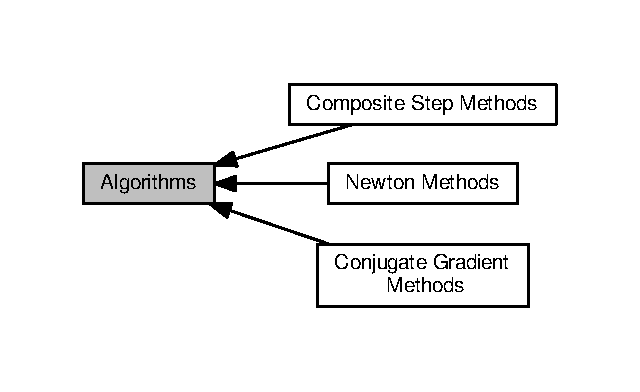
\includegraphics[width=308pt]{group__AlgorithmGroup}
\end{center}
\end{figure}
\subsection*{Modules}
\begin{DoxyCompactItemize}
\item 
\hyperlink{group__NewtonGroup}{Newton Methods}
\begin{DoxyCompactList}\small\item\em Newton methods, largely following \cite{Deuflhard2004}. \end{DoxyCompactList}\item 
\hyperlink{group__CGGroup}{Conjugate Gradient Methods}
\begin{DoxyCompactList}\small\item\em Conjugate gradient methods for convex and nonconvex problems (C\-G, Truncated C\-G, Regularized C\-G and Truncated Regularized C\-G). \end{DoxyCompactList}\item 
\hyperlink{group__CSGroup}{Composite Step Methods}
\begin{DoxyCompactList}\small\item\em Contains the affine covariant composite step method of \cite{Lubkoll2015}, \cite{Lubkoll2015a}. \end{DoxyCompactList}\end{DoxyCompactItemize}


\subsection{Detailed Description}
Contains different algorithms that can be formulated in vector spaces. Contains different variants of conjugate gradient methods for convex and nonconvex problems, different newton methods and an affine covariant composite step method. 
\hypertarget{group__NewtonGroup}{\section{\-Newton \-Methods}
\label{group__NewtonGroup}\index{\-Newton Methods@{\-Newton Methods}}
}


\-Newton methods, largely following  


\-Collaboration diagram for \-Newton \-Methods\-:
\nopagebreak
\begin{figure}[H]
\begin{center}
\leavevmode
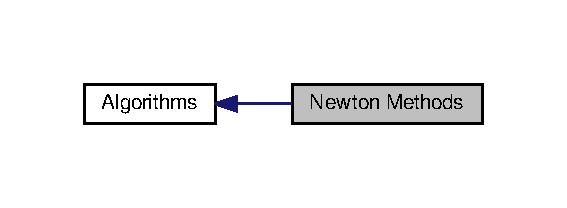
\includegraphics[width=272pt]{group__NewtonGroup}
\end{center}
\end{figure}
\subsection*{\-Classes}
\begin{DoxyCompactItemize}
\item 
class \hyperlink{classSpacy_1_1Newton_1_1Damping_1_1AffineCovariant}{\-Spacy\-::\-Newton\-::\-Damping\-::\-Affine\-Covariant}
\begin{DoxyCompactList}\small\item\em \-Affine covariant damping strategy as described in. \end{DoxyCompactList}\item 
class \hyperlink{classSpacy_1_1Newton_1_1Damping_1_1AffineContravariant}{\-Spacy\-::\-Newton\-::\-Damping\-::\-Affine\-Contravariant}
\begin{DoxyCompactList}\small\item\em \-Affine contravariant damping strategy as described in. \end{DoxyCompactList}\item 
class \hyperlink{classSpacy_1_1Newton_1_1Damping_1_1None}{\-Spacy\-::\-Newton\-::\-Damping\-::\-None}
\begin{DoxyCompactList}\small\item\em \-No damping, yields local newton method. \end{DoxyCompactList}\end{DoxyCompactItemize}
\subsection*{\-Namespaces}
\begin{DoxyCompactItemize}
\item 
namespace \hyperlink{namespaceSpacy_1_1Newton}{\-Spacy\-::\-Newton}
\begin{DoxyCompactList}\small\item\em \-Newton methods, largely following \end{DoxyCompactList}\end{DoxyCompactItemize}
\subsection*{\-Functions}
\begin{DoxyCompactItemize}
\item 
\-Vector \hyperlink{group__NewtonGroup_ga448b8e78b2e84ed78e70c42114ea7599}{\-Spacy\-::local\-Newton} (const \-C1\-Operator \&\-F, const \-Vector \&x0, const \-Newton\-::\-Parameter \&p=\-Newton\-::\-Parameter())
\begin{DoxyCompactList}\small\item\em \-Local \-Newton method. \end{DoxyCompactList}\item 
\-Vector \hyperlink{group__NewtonGroup_gafbe5e25f46f7b0d237f5e9971cef998a}{\-Spacy\-::local\-Newton} (const \-C1\-Operator \&\-F, const \-Newton\-::\-Parameter \&p=\-Newton\-::\-Parameter())
\begin{DoxyCompactList}\small\item\em \-Local \-Newton method with default initial iterate (x0=0). \end{DoxyCompactList}\item 
\-Vector \hyperlink{group__NewtonGroup_ga6c18ad252cb530e4f6734eb4e4fda481}{\-Spacy\-::covariant\-Newton} (const \-C1\-Operator \&\-F, const \-Vector \&x0, const \-Newton\-::\-Parameter \&p=\-Newton\-::\-Parameter(), const std\-::function$<$ bool(const \-Vector \&, const \-Vector \&)$>$ \&error\-Estimator=\{\})
\begin{DoxyCompactList}\small\item\em \-Affine covariant \-Newton method. \end{DoxyCompactList}\item 
\-Vector \hyperlink{group__NewtonGroup_ga2d469322482680319bf81d865ed57068}{\-Spacy\-::covariant\-Newton} (const \-C1\-Operator \&\-F, const \-Newton\-::\-Parameter \&p=\-Newton\-::\-Parameter(), const std\-::function$<$ bool(const \-Vector \&, const \-Vector \&)$>$ \&error\-Estimator=\{\})
\begin{DoxyCompactList}\small\item\em \-Affine covariant \-Newton method. \end{DoxyCompactList}\item 
\-Vector \hyperlink{group__NewtonGroup_gaa32f667c573986b2b2721ec6532fc832}{\-Spacy\-::contravariant\-Newton} (const \-C1\-Operator \&\-F, const \-Vector \&x0, const \-Newton\-::\-Parameter \&p=\-Newton\-::\-Parameter())
\begin{DoxyCompactList}\small\item\em \-Affine contravariant \-Newton method. \end{DoxyCompactList}\item 
\-Vector \hyperlink{group__NewtonGroup_gace045630c7f0c7a1a5a48d2d0807f608}{\-Spacy\-::contravariant\-Newton} (const \-C1\-Operator \&\-F, const \-Newton\-::\-Parameter \&p=\-Newton\-::\-Parameter())
\begin{DoxyCompactList}\small\item\em \-Affine contravariant \-Newton method. \end{DoxyCompactList}\end{DoxyCompactItemize}


\subsection{\-Detailed \-Description}
\-Newton methods, largely following \cite{Deuflhard2004}.

\-Contains a local \-Newton method, an affine covariant \-Newton method, an affine contravariant \-Newton method as well as a generic implementation that admits the implementation of further termination criteria and damping strategies. 

\subsection{\-Function \-Documentation}
\hypertarget{group__NewtonGroup_ga448b8e78b2e84ed78e70c42114ea7599}{\index{\-Newton Methods@{\-Newton Methods}!local\-Newton@{local\-Newton}}
\index{local\-Newton@{local\-Newton}!Newton Methods@{\-Newton Methods}}
\subsubsection[{local\-Newton}]{\setlength{\rightskip}{0pt plus 5cm}\-Vector {\bf \-Spacy\-::local\-Newton} (
\begin{DoxyParamCaption}
\item[{const \-C1\-Operator \&}]{\-F, }
\item[{const \-Vector \&}]{x0, }
\item[{const \-Newton\-::\-Parameter \&}]{p = {\ttfamily \-Newton\-:\-:\-Parameter()}}
\end{DoxyParamCaption}
)}}\label{group__NewtonGroup_ga448b8e78b2e84ed78e70c42114ea7599}


\-Local \-Newton method. 


\begin{DoxyParams}{\-Parameters}
{\em \-F} & operator \\
\hline
{\em x0} & initial iterate \\
\hline
{\em p} & parameter object holding algorithmic parameters\\
\hline
\end{DoxyParams}

\begin{DoxyItemize}
\item \-Damping strategy\-: \-Newton\-::\-Damping\-Strategy\-::\-None
\item \-Termination criterion\-: \-Newton\-::\-Termination\-Criterion\-::\-Affine\-Covariant
\end{DoxyItemize}

\begin{DoxySeeAlso}{\-See also}
\hyperlink{structSpacy_1_1Newton_1_1Parameter}{\-Newton\-::\-Parameter} 
\end{DoxySeeAlso}
\hypertarget{group__NewtonGroup_gafbe5e25f46f7b0d237f5e9971cef998a}{\index{\-Newton Methods@{\-Newton Methods}!local\-Newton@{local\-Newton}}
\index{local\-Newton@{local\-Newton}!Newton Methods@{\-Newton Methods}}
\subsubsection[{local\-Newton}]{\setlength{\rightskip}{0pt plus 5cm}\-Vector {\bf \-Spacy\-::local\-Newton} (
\begin{DoxyParamCaption}
\item[{const \-C1\-Operator \&}]{\-F, }
\item[{const \-Newton\-::\-Parameter \&}]{p = {\ttfamily \-Newton\-:\-:\-Parameter()}}
\end{DoxyParamCaption}
)}}\label{group__NewtonGroup_gafbe5e25f46f7b0d237f5e9971cef998a}


\-Local \-Newton method with default initial iterate (x0=0). 


\begin{DoxyParams}{\-Parameters}
{\em \-F} & operator \\
\hline
{\em p} & parameter object holding algorithmic parameters\\
\hline
\end{DoxyParams}

\begin{DoxyItemize}
\item \-Damping strategy\-: \-Newton\-::\-Damping\-Strategy\-::\-None
\item \-Termination criterion\-: \-Newton\-::\-Termination\-Criterion\-::\-Affine\-Covariant
\end{DoxyItemize}

\begin{DoxySeeAlso}{\-See also}
\hyperlink{structSpacy_1_1Newton_1_1Parameter}{\-Newton\-::\-Parameter} 
\end{DoxySeeAlso}
\hypertarget{group__NewtonGroup_ga6c18ad252cb530e4f6734eb4e4fda481}{\index{\-Newton Methods@{\-Newton Methods}!covariant\-Newton@{covariant\-Newton}}
\index{covariant\-Newton@{covariant\-Newton}!Newton Methods@{\-Newton Methods}}
\subsubsection[{covariant\-Newton}]{\setlength{\rightskip}{0pt plus 5cm}\-Vector {\bf \-Spacy\-::covariant\-Newton} (
\begin{DoxyParamCaption}
\item[{const \-C1\-Operator \&}]{\-F, }
\item[{const \-Vector \&}]{x0, }
\item[{const \-Newton\-::\-Parameter \&}]{p = {\ttfamily \-Newton\-:\-:\-Parameter()}}
\end{DoxyParamCaption}
)}}\label{group__NewtonGroup_ga6c18ad252cb530e4f6734eb4e4fda481}


\-Affine covariant \-Newton method. 


\begin{DoxyParams}{\-Parameters}
{\em \-F} & operator \\
\hline
{\em x0} & initial iterate \\
\hline
{\em p} & parameter object holding algorithmic parameters\\
\hline
\end{DoxyParams}

\begin{DoxyItemize}
\item \-Damping strategy\-: \-Newton\-::\-Damping\-Strategy\-::\-Affine\-Covariant
\item \-Termination criterion\-: \-Newton\-::\-Termination\-Criterion\-::\-Affine\-Covariant
\end{DoxyItemize}

\begin{DoxySeeAlso}{\-See also}
\hyperlink{structSpacy_1_1Newton_1_1Parameter}{\-Newton\-::\-Parameter} 
\end{DoxySeeAlso}
\hypertarget{group__NewtonGroup_ga2d469322482680319bf81d865ed57068}{\index{\-Newton Methods@{\-Newton Methods}!covariant\-Newton@{covariant\-Newton}}
\index{covariant\-Newton@{covariant\-Newton}!Newton Methods@{\-Newton Methods}}
\subsubsection[{covariant\-Newton}]{\setlength{\rightskip}{0pt plus 5cm}\-Vector {\bf \-Spacy\-::covariant\-Newton} (
\begin{DoxyParamCaption}
\item[{const \-C1\-Operator \&}]{\-F, }
\item[{const \-Newton\-::\-Parameter \&}]{p = {\ttfamily \-Newton\-:\-:\-Parameter()}}
\end{DoxyParamCaption}
)}}\label{group__NewtonGroup_ga2d469322482680319bf81d865ed57068}


\-Affine covariant \-Newton method. 


\begin{DoxyParams}{\-Parameters}
{\em \-F} & operator \\
\hline
{\em p} & parameter object holding algorithmic parameters\\
\hline
\end{DoxyParams}

\begin{DoxyItemize}
\item \-Damping strategy\-: \-Newton\-::\-Damping\-Strategy\-::\-Affine\-Covariant
\item \-Termination criterion\-: \-Newton\-::\-Termination\-Criterion\-::\-Affine\-Covariant
\end{DoxyItemize}

\begin{DoxySeeAlso}{\-See also}
\hyperlink{structSpacy_1_1Newton_1_1Parameter}{\-Newton\-::\-Parameter} 
\end{DoxySeeAlso}
\hypertarget{group__NewtonGroup_gaa32f667c573986b2b2721ec6532fc832}{\index{\-Newton Methods@{\-Newton Methods}!contravariant\-Newton@{contravariant\-Newton}}
\index{contravariant\-Newton@{contravariant\-Newton}!Newton Methods@{\-Newton Methods}}
\subsubsection[{contravariant\-Newton}]{\setlength{\rightskip}{0pt plus 5cm}\-Vector {\bf \-Spacy\-::contravariant\-Newton} (
\begin{DoxyParamCaption}
\item[{const \-C1\-Operator \&}]{\-F, }
\item[{const \-Vector \&}]{x0, }
\item[{const \-Newton\-::\-Parameter \&}]{p = {\ttfamily \-Newton\-:\-:\-Parameter()}}
\end{DoxyParamCaption}
)}}\label{group__NewtonGroup_gaa32f667c573986b2b2721ec6532fc832}


\-Affine contravariant \-Newton method. 


\begin{DoxyParams}{\-Parameters}
{\em \-F} & operator \\
\hline
{\em x0} & initial iterate \\
\hline
{\em p} & parameter object holding algorithmic parameters\\
\hline
\end{DoxyParams}

\begin{DoxyItemize}
\item \-Damping strategy\-: \-Newton\-::\-Damping\-Strategy\-::\-Affine\-Contravariant
\item \-Termination criterion\-: \-Newton\-::\-Termination\-Criterion\-::\-Affine\-Contravariant
\end{DoxyItemize}

\begin{DoxySeeAlso}{\-See also}
\hyperlink{structSpacy_1_1Newton_1_1Parameter}{\-Newton\-::\-Parameter} 
\end{DoxySeeAlso}
\hypertarget{group__NewtonGroup_gace045630c7f0c7a1a5a48d2d0807f608}{\index{\-Newton Methods@{\-Newton Methods}!contravariant\-Newton@{contravariant\-Newton}}
\index{contravariant\-Newton@{contravariant\-Newton}!Newton Methods@{\-Newton Methods}}
\subsubsection[{contravariant\-Newton}]{\setlength{\rightskip}{0pt plus 5cm}\-Vector {\bf \-Spacy\-::contravariant\-Newton} (
\begin{DoxyParamCaption}
\item[{const \-C1\-Operator \&}]{\-F, }
\item[{const \-Newton\-::\-Parameter \&}]{p = {\ttfamily \-Newton\-:\-:\-Parameter()}}
\end{DoxyParamCaption}
)}}\label{group__NewtonGroup_gace045630c7f0c7a1a5a48d2d0807f608}


\-Affine contravariant \-Newton method. 


\begin{DoxyParams}{\-Parameters}
{\em \-F} & operator \\
\hline
{\em p} & parameter object holding algorithmic parameters\\
\hline
\end{DoxyParams}

\begin{DoxyItemize}
\item \-Damping strategy\-: \-Newton\-::\-Damping\-Strategy\-::\-Affine\-Contravariant
\item \-Termination criterion\-: \-Newton\-::\-Termination\-Criterion\-::\-Affine\-Contravariant
\end{DoxyItemize}

\begin{DoxySeeAlso}{\-See also}
\hyperlink{structSpacy_1_1Newton_1_1Parameter}{\-Newton\-::\-Parameter} 
\end{DoxySeeAlso}

\hypertarget{group__CGGroup}{}\section{Conjugate Gradient Methods}
\label{group__CGGroup}\index{Conjugate Gradient Methods@{Conjugate Gradient Methods}}


Conjugate gradient methods for convex and nonconvex problems (CG, Truncated CG, Regularized CG and Truncated Regularized CG).  


Collaboration diagram for Conjugate Gradient Methods\+:
\nopagebreak
\begin{figure}[H]
\begin{center}
\leavevmode
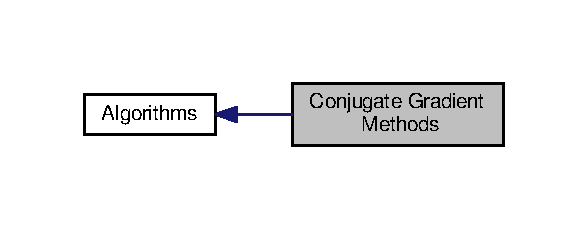
\includegraphics[width=280pt]{group__CGGroup}
\end{center}
\end{figure}
\subsection*{Namespaces}
\begin{DoxyCompactItemize}
\item 
 \hyperlink{namespaceSpacy_1_1CG}{Spacy\+::\+CG}
\begin{DoxyCompactList}\small\item\em Conjugate gradient methods for convex and nonconvex problems (CG, Truncated CG, Regularized CG and Truncated Regularized CG). \end{DoxyCompactList}\end{DoxyCompactItemize}
\subsection*{Classes}
\begin{DoxyCompactItemize}
\item 
class \hyperlink{classSpacy_1_1CG_1_1Solver}{Spacy\+::\+C\+G\+::\+Solver}
\begin{DoxyCompactList}\small\item\em Conjugate gradient method. \end{DoxyCompactList}\end{DoxyCompactItemize}


\subsection{Detailed Description}
Conjugate gradient methods for convex and nonconvex problems (CG, Truncated CG, Regularized CG and Truncated Regularized CG). 


\hypertarget{group__CSGroup}{\section{Composite Step Methods}
\label{group__CSGroup}\index{Composite Step Methods@{Composite Step Methods}}
}


Contains the affine covariant composite step method of \cite{Lubkoll2015}, \cite{Lubkoll2015a}.  


Collaboration diagram for Composite Step Methods\-:
\nopagebreak
\begin{figure}[H]
\begin{center}
\leavevmode
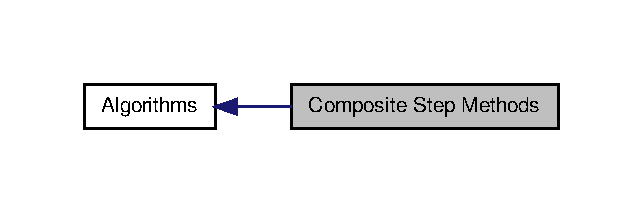
\includegraphics[width=308pt]{group__CSGroup}
\end{center}
\end{figure}
\subsection*{Classes}
\begin{DoxyCompactItemize}
\item 
class \hyperlink{classSpacy_1_1CompositeStep_1_1AffineCovariantSolver}{Spacy\-::\-Composite\-Step\-::\-Affine\-Covariant\-Solver}
\begin{DoxyCompactList}\small\item\em The affine covariant step method described in \cite{Lubkoll2015}, \cite{Lubkoll2015a} for the solution of equality constraint optimization problems. \end{DoxyCompactList}\end{DoxyCompactItemize}


\subsection{Detailed Description}
Contains the affine covariant composite step method of \cite{Lubkoll2015}, \cite{Lubkoll2015a}. 
\hypertarget{group__ConceptGroup}{\section{\-Concepts}
\label{group__ConceptGroup}\index{\-Concepts@{\-Concepts}}
}


\-Concepts for vectors, functionals, operators, ...  


\-Concepts for vectors, functionals, operators, ... 
\chapter{\-Namespace \-Documentation}
\hypertarget{namespaceSpacy}{\section{\-Spacy \-Namespace \-Reference}
\label{namespaceSpacy}\index{\-Spacy@{\-Spacy}}
}


\-Main namespace of the \-Spacy library.  


\subsection*{\-Namespaces}
\begin{DoxyCompactItemize}
\item 
namespace \hyperlink{namespaceSpacy_1_1CG}{\-C\-G}
\begin{DoxyCompactList}\small\item\em \-Conjugate gradient methods for convex and nonconvex problems (\-C\-G, \-Truncated \-C\-G, \-Regularized \-C\-G and \-Truncated \-Regularized \-C\-G). \end{DoxyCompactList}\item 
namespace \hyperlink{namespaceSpacy_1_1Newton}{\-Newton}
\begin{DoxyCompactList}\small\item\em \-Newton methods, largely following \end{DoxyCompactList}\item 
namespace \hyperlink{namespaceSpacy_1_1CompositeStep}{\-Composite\-Step}
\begin{DoxyCompactList}\small\item\em \-Contains the affine covariant composite step method of. \end{DoxyCompactList}\item 
namespace \hyperlink{namespaceSpacy_1_1ProductSpace}{\-Product\-Space}
\begin{DoxyCompactList}\small\item\em \-A product space that supports distinction between primal and dual variables. \end{DoxyCompactList}\item 
namespace \hyperlink{namespaceSpacy_1_1FEniCS}{\-F\-Eni\-C\-S}
\begin{DoxyCompactList}\small\item\em \-Contains vector spaces, functionals and operators for \href{www.fenicsproject.org}{\tt \-F\-Eni\-C\-S}. \end{DoxyCompactList}\item 
namespace \hyperlink{namespaceSpacy_1_1Kaskade}{\-Kaskade}
\begin{DoxyCompactList}\small\item\em \-Contains vector spaces, functionals and operators for \href{http://www.zib.de/projects/kaskade7-finite-element-toolbox}{\tt \-Kaskade7}. \end{DoxyCompactList}\item 
namespace \hyperlink{namespaceSpacy_1_1Scalar}{\-Scalar}
\begin{DoxyCompactList}\small\item\em \-Contains functionals and operators for scalar problems. \end{DoxyCompactList}\item 
namespace \hyperlink{namespaceSpacy_1_1Rn}{\-Rn}
\begin{DoxyCompactList}\small\item\em \-Contains functionals and operators for finite dimensional vector space problems, based on \href{http://eigen.tuxfamily.org}{\tt \-Eigen}. \end{DoxyCompactList}\item 
namespace \hyperlink{namespaceSpacy_1_1Generic}{\-Generic}
\begin{DoxyCompactList}\small\item\em \-Contains generic implementations for easier definitions of vectors and a generic scalar product implementation. \end{DoxyCompactList}\item 
namespace \hyperlink{namespaceSpacy_1_1Mixin}{\-Mixin}
\begin{DoxyCompactList}\small\item\em \-Contains small independent components that are frequently used and can be added to classes via (multiple) inheritance. \end{DoxyCompactList}\item 
namespace \hyperlink{namespaceSpacy_1_1Optional}{\-Optional}
\item 
namespace \hyperlink{namespaceSpacy_1_1Detail}{\-Detail}
\end{DoxyCompactItemize}
\subsection*{\-Classes}
\begin{DoxyCompactItemize}
\item 
class \hyperlink{classSpacy_1_1C1Functional}{\-C1\-Functional}
\begin{DoxyCompactList}\small\item\em \-Type-\/erased differentiable functional $f:\ X \to \mathbb{R} $. \end{DoxyCompactList}\item 
class \hyperlink{classSpacy_1_1C1Operator}{\-C1\-Operator}
\begin{DoxyCompactList}\small\item\em \-Type-\/erased differentiable operator $A:\ X \to Y $. \end{DoxyCompactList}\item 
class \hyperlink{classSpacy_1_1C2Functional}{\-C2\-Functional}
\begin{DoxyCompactList}\small\item\em \-Type-\/erased twice differentiable functional $f:\ X \to \mathbb{R} $. \end{DoxyCompactList}\item 
class \hyperlink{classSpacy_1_1DynamicOperator}{\-Dynamic\-Operator}
\begin{DoxyCompactList}\small\item\em \-Type-\/erased time-\/dependent operator $A:\ [0,T] \times X \to Y $. \end{DoxyCompactList}\item 
class \hyperlink{classSpacy_1_1DynamicLinearOperator}{\-Dynamic\-Linear\-Operator}
\begin{DoxyCompactList}\small\item\em \-Type-\/erased time-\/dependent linear operator $A:\ [0,T] \times X \to Y $. \end{DoxyCompactList}\item 
class \hyperlink{classSpacy_1_1DynamicC1Operator}{\-Dynamic\-C1\-Operator}
\begin{DoxyCompactList}\small\item\em \-Type-\/erased time-\/dependent differentiable operator $A:\ [0,T] \times X \to Y $. \end{DoxyCompactList}\item 
class \hyperlink{classSpacy_1_1Functional}{\-Functional}
\begin{DoxyCompactList}\small\item\em \-Type-\/erased functional $f:\ X \to \mathbb{R} $. \end{DoxyCompactList}\item 
class \hyperlink{classSpacy_1_1LinearOperator}{\-Linear\-Operator}
\begin{DoxyCompactList}\small\item\em \-Type-\/erased linear operator $A:\ X \to Y $. \end{DoxyCompactList}\item 
class \hyperlink{classSpacy_1_1IndefiniteLinearSolver}{\-Indefinite\-Linear\-Solver}
\begin{DoxyCompactList}\small\item\em \-Type-\/erased indefinite linear solver. \-Additionally monitors if the underlying operator is positive definite. \end{DoxyCompactList}\item 
class \hyperlink{classSpacy_1_1Operator}{\-Operator}
\begin{DoxyCompactList}\small\item\em \-Type-\/erased operator $A:\ X \to Y $. \end{DoxyCompactList}\item 
class \hyperlink{classSpacy_1_1Vector}{\-Vector}
\begin{DoxyCompactList}\small\item\em \-Type-\/erased vector. \end{DoxyCompactList}\item 
class \hyperlink{classSpacy_1_1ZeroVectorCreator}{\-Zero\-Vector\-Creator}
\begin{DoxyCompactList}\small\item\em \-Each \hyperlink{classSpacy_1_1VectorSpace}{\-Vector\-Space} needs a zero-\/vector creator to support generation of vector space elements. \end{DoxyCompactList}\item 
class \hyperlink{classSpacy_1_1DampingFactor}{\-Damping\-Factor}
\begin{DoxyCompactList}\small\item\em \-A simple model of a damping factor $\nu$ that is computed up to a prescribed accuracy $\varepsilon$. \end{DoxyCompactList}\item 
class \hyperlink{classSpacy_1_1LipschitzConstant}{\-Lipschitz\-Constant}
\begin{DoxyCompactList}\small\item\em \-A simple model for a \-Lipschitz constant $\omega$. \end{DoxyCompactList}\item 
class \hyperlink{classSpacy_1_1Parameter}{\-Parameter}
\begin{DoxyCompactList}\small\item\em \-Basic parameters for simple algorithms. \end{DoxyCompactList}\item 
class \hyperlink{classSpacy_1_1HilbertSpaceNorm}{\-Hilbert\-Space\-Norm}
\begin{DoxyCompactList}\small\item\em $ \|\cdot\|=\sqrt{(\cdot,\cdot)} $ \end{DoxyCompactList}\item 
class \hyperlink{classSpacy_1_1AdaptiveInducedScalarProduct}{\-Adaptive\-Induced\-Scalar\-Product}
\begin{DoxyCompactList}\small\item\em \-Induced scalar product $(x,y)_M = (Mx)y$, where $M:X\rightarrow X^*$. \end{DoxyCompactList}\item 
class \hyperlink{classSpacy_1_1InducedScalarProduct}{\-Induced\-Scalar\-Product}
\begin{DoxyCompactList}\small\item\em \-Induced scalar product $(x,y)_M = (Mx)y$, where $M:X\rightarrow X^*$. \end{DoxyCompactList}\item 
class \hyperlink{classSpacy_1_1PrimalInducedScalarProduct}{\-Primal\-Induced\-Scalar\-Product}
\begin{DoxyCompactList}\small\item\em \-Induced scalar product for the primal variables (i.\-e. for constrained optimization problems). \end{DoxyCompactList}\item 
class \hyperlink{classSpacy_1_1Real}{\-Real}
\begin{DoxyCompactList}\small\item\em \-Real number. \end{DoxyCompactList}\item 
class \hyperlink{classSpacy_1_1AddArithmeticOperators}{\-Add\-Arithmetic\-Operators}
\begin{DoxyCompactList}\small\item\em \-Base class providing some operations for vectors via \-C\-R\-T\-P. \end{DoxyCompactList}\item 
class \hyperlink{classSpacy_1_1FunctionalBase}{\-Functional\-Base}
\item 
class \hyperlink{classSpacy_1_1OperatorBase}{\-Operator\-Base}
\item 
class \hyperlink{classSpacy_1_1VectorBase}{\-Vector\-Base}
\begin{DoxyCompactList}\small\item\em \-Base class for vector implementations. \end{DoxyCompactList}\item 
class \hyperlink{classSpacy_1_1CallOfUndefinedFunctionException}{\-Call\-Of\-Undefined\-Function\-Exception}
\begin{DoxyCompactList}\small\item\em \-Exception to be thrown if a virtual function is not implemented. \end{DoxyCompactList}\item 
class \hyperlink{classSpacy_1_1GenericException}{\-Generic\-Exception}
\begin{DoxyCompactList}\small\item\em \-A generic exception class that serves as base for all exceptions in this library. \end{DoxyCompactList}\item 
class \hyperlink{classSpacy_1_1IncompatibleSpaceException}{\-Incompatible\-Space\-Exception}
\begin{DoxyCompactList}\small\item\em \-Exception to be thrown when encountering incompatible spaces. \end{DoxyCompactList}\item 
class \hyperlink{classSpacy_1_1RegularityTestFailedException}{\-Regularity\-Test\-Failed\-Exception}
\begin{DoxyCompactList}\small\item\em \-Exception to be thrown if regularity test fails. \end{DoxyCompactList}\item 
class \hyperlink{classSpacy_1_1SingularOperatorException}{\-Singular\-Operator\-Exception}
\begin{DoxyCompactList}\small\item\em \-Exception to be thrown if singular operators are inverted. \end{DoxyCompactList}\item 
struct \hyperlink{structSpacy_1_1Logger}{\-Logger}
\item 
struct \hyperlink{structSpacy_1_1IsVoid}{\-Is\-Void}
\item 
struct \hyperlink{structSpacy_1_1Require}{\-Require}
\begin{DoxyCompactList}\small\item\em \-Check if \-Concept is satisfied. \end{DoxyCompactList}\item 
class \hyperlink{classSpacy_1_1VectorSpace}{\-Vector\-Space}
\begin{DoxyCompactList}\small\item\em \-Function space $(X,\|\cdot\|)$. \end{DoxyCompactList}\end{DoxyCompactItemize}
\subsection*{\-Enumerations}
\begin{DoxyCompactItemize}
\item 
enum \{ {\bfseries \-P\-R\-I\-M\-A\-L} = 0, 
{\bfseries \-D\-U\-A\-L} = 1
 \}
\end{DoxyCompactItemize}
\subsection*{\-Functions}
\begin{DoxyCompactItemize}
\item 
\hyperlink{classSpacy_1_1LinearOperator}{\-Linear\-Operator} \hyperlink{namespaceSpacy_a2205e2a2c4bb5242665bbc09929d35d2}{d1} (const \hyperlink{classSpacy_1_1C1Operator}{\-C1\-Operator} \&\-A, const \hyperlink{classSpacy_1_1Vector}{\-Vector} \&x)
\begin{DoxyCompactList}\small\item\em \-For an operator $ A: X\to Y $, compute $A'$ at $x\in X$ as linear operator $ A'(x): X \to Y $. \end{DoxyCompactList}\item 
\hyperlink{classSpacy_1_1Vector}{\-Vector} \hyperlink{namespaceSpacy_ab6646eb7068eb9f1369e639cf0b620a2}{d1} (const \hyperlink{classSpacy_1_1C2Functional}{\-C2\-Functional} \&f, const \hyperlink{classSpacy_1_1Vector}{\-Vector} \&x)
\begin{DoxyCompactList}\small\item\em \-For a functional $ f: X\to \mathbb{R} $, compute $f'$ at $x\in X$ as dual element $ f'(x) \in X^* $. \end{DoxyCompactList}\item 
\hyperlink{classSpacy_1_1LinearOperator}{\-Linear\-Operator} \hyperlink{namespaceSpacy_a569d8fc0b4a0e292f257dd6307a25c8f}{d2} (const \hyperlink{classSpacy_1_1C2Functional}{\-C2\-Functional} \&f, const \hyperlink{classSpacy_1_1Vector}{\-Vector} \&x)
\begin{DoxyCompactList}\small\item\em \-For a functional $ f: X\to \mathbb{R} $, compute $f''$ at $x\in X$ as linear operator $ f''(x): X \to X^* $. \end{DoxyCompactList}\item 
\hypertarget{namespaceSpacy_ab1be097dacbf27785979de79ed5b3178}{\-Linear\-Solver \hyperlink{namespaceSpacy_ab1be097dacbf27785979de79ed5b3178}{operator$^\wedge$} (const \hyperlink{classSpacy_1_1LinearOperator}{\-Linear\-Operator} \&\-A, int k)}\label{namespaceSpacy_ab1be097dacbf27785979de79ed5b3178}

\begin{DoxyCompactList}\small\item\em \-Access solver via \-A$^\wedge$-\/1. \-Throws for k!=-\/1. \end{DoxyCompactList}\item 
\hypertarget{namespaceSpacy_a6defec6ee302bf4c1054afc65c9fcb95}{\-Linear\-Solver \hyperlink{namespaceSpacy_a6defec6ee302bf4c1054afc65c9fcb95}{operator$^\wedge$} (\hyperlink{classSpacy_1_1LinearOperator}{\-Linear\-Operator} \&\&\-A, int k)}\label{namespaceSpacy_a6defec6ee302bf4c1054afc65c9fcb95}

\begin{DoxyCompactList}\small\item\em \-Access solver via \-A$^\wedge$-\/1. \-Throws for k!=-\/1. \end{DoxyCompactList}\item 
\hypertarget{namespaceSpacy_ad08055ec05275c6042d516d4726b5e8f}{\hyperlink{classSpacy_1_1LinearOperator}{\-Linear\-Operator} \& {\bfseries axpy} (\hyperlink{classSpacy_1_1LinearOperator}{\-Linear\-Operator} \&\-A, double a, \hyperlink{classSpacy_1_1LinearOperator}{\-Linear\-Operator} \-B)}\label{namespaceSpacy_ad08055ec05275c6042d516d4726b5e8f}

\item 
\hypertarget{namespaceSpacy_ae0a1cbb3d98d6ac0a82727959038f4b4}{{\footnotesize template$<$class Arithmetic , class  = std\-::enable\-\_\-if\-\_\-t$<$ std\-::is\-\_\-arithmetic$<$\-Arithmetic$>$\-::value $>$$>$ }\\\hyperlink{classSpacy_1_1Vector}{\-Vector} \hyperlink{namespaceSpacy_ae0a1cbb3d98d6ac0a82727959038f4b4}{operator$\ast$} (\-Arithmetic a, \hyperlink{classSpacy_1_1Vector}{\-Vector} x)}\label{namespaceSpacy_ae0a1cbb3d98d6ac0a82727959038f4b4}

\begin{DoxyCompactList}\small\item\em \-Multiplication with arithmetic types (double,float,int,...). \end{DoxyCompactList}\item 
\hypertarget{namespaceSpacy_a0120fd6b1d7580a9f7b8f24e646cbc6c}{{\footnotesize template$<$class Arithmetic , class  = std\-::enable\-\_\-if\-\_\-t$<$ std\-::is\-\_\-arithmetic$<$\-Arithmetic$>$\-::value $>$$>$ }\\\hyperlink{classSpacy_1_1Vector}{\-Vector} \hyperlink{namespaceSpacy_a0120fd6b1d7580a9f7b8f24e646cbc6c}{operator$\ast$} (\hyperlink{classSpacy_1_1Vector}{\-Vector} x, \-Arithmetic a)}\label{namespaceSpacy_a0120fd6b1d7580a9f7b8f24e646cbc6c}

\begin{DoxyCompactList}\small\item\em \-Multiplication with arithmetic types (double,float,int,...). \end{DoxyCompactList}\item 
\hypertarget{namespaceSpacy_a19486acb05af1627ec49c376b204a61c}{\hyperlink{classSpacy_1_1Vector}{\-Vector} \hyperlink{namespaceSpacy_a19486acb05af1627ec49c376b204a61c}{operator+} (\hyperlink{classSpacy_1_1Vector}{\-Vector} x, const \hyperlink{classSpacy_1_1Vector}{\-Vector} \&y)}\label{namespaceSpacy_a19486acb05af1627ec49c376b204a61c}

\begin{DoxyCompactList}\small\item\em \-Sum of vectors $z=x+y$. \end{DoxyCompactList}\item 
\hypertarget{namespaceSpacy_a9eaf4be1a4e8f3ee03e4c4fdafa5687d}{\hyperlink{classSpacy_1_1Vector}{\-Vector} \hyperlink{namespaceSpacy_a9eaf4be1a4e8f3ee03e4c4fdafa5687d}{operator-\/} (\hyperlink{classSpacy_1_1Vector}{\-Vector} x, const \hyperlink{classSpacy_1_1Vector}{\-Vector} \&y)}\label{namespaceSpacy_a9eaf4be1a4e8f3ee03e4c4fdafa5687d}

\begin{DoxyCompactList}\small\item\em \-Subtract vectors $z=x-y$. \end{DoxyCompactList}\item 
\hypertarget{namespaceSpacy_a1d84603fc2bfbefca6a020b1217519ad}{\hyperlink{classSpacy_1_1Real}{\-Real} \hyperlink{namespaceSpacy_a1d84603fc2bfbefca6a020b1217519ad}{operator$\ast$} (const \hyperlink{classSpacy_1_1Vector}{\-Vector} \&x, const \hyperlink{classSpacy_1_1Vector}{\-Vector} \&y)}\label{namespaceSpacy_a1d84603fc2bfbefca6a020b1217519ad}

\begin{DoxyCompactList}\small\item\em \-Compute scalar product $z=x*y=(x,y)$. \end{DoxyCompactList}\item 
\hypertarget{namespaceSpacy_a86a4fc266aa19a07b0af16388907354b}{\hyperlink{classSpacy_1_1Real}{\-Real} \hyperlink{namespaceSpacy_a86a4fc266aa19a07b0af16388907354b}{norm} (const \hyperlink{classSpacy_1_1Vector}{\-Vector} \&x)}\label{namespaceSpacy_a86a4fc266aa19a07b0af16388907354b}

\begin{DoxyCompactList}\small\item\em \-Compute norm, where the norm associated with the underlying function space is used $ z = \|x\| $. \end{DoxyCompactList}\item 
\hypertarget{namespaceSpacy_ac354f06d21282619482e3ef4a841cd76}{void {\bfseries check\-Dual\-Pairing} (const \hyperlink{classSpacy_1_1Vector}{\-Vector} \&x, const \hyperlink{classSpacy_1_1Vector}{\-Vector} \&y)}\label{namespaceSpacy_ac354f06d21282619482e3ef4a841cd76}

\item 
\hypertarget{namespaceSpacy_a0e5e7a61e6d2996df2b3e86371d38dfa}{{\footnotesize template$<$class T , typename std\-::enable\-\_\-if$<$ std\-::is\-\_\-arithmetic$<$ T $>$\-::value $>$\-::type $\ast$  = nullptr$>$ }\\\hyperlink{classSpacy_1_1Vector}{\-Vector} {\bfseries operator$\ast$} (const \-Mixin\-::\-Get$<$ \-T $>$ \&x, \hyperlink{classSpacy_1_1Vector}{\-Vector} y)}\label{namespaceSpacy_a0e5e7a61e6d2996df2b3e86371d38dfa}

\item 
\hypertarget{namespaceSpacy_a6656b636307ec4d5552477027b724f46}{{\footnotesize template$<$class T , typename std\-::enable\-\_\-if$<$ std\-::is\-\_\-arithmetic$<$ T $>$\-::value $>$\-::type $\ast$  = nullptr$>$ }\\\hyperlink{classSpacy_1_1Vector}{\-Vector} {\bfseries operator$\ast$} (const \hyperlink{classSpacy_1_1Vector}{\-Vector} \&x, const \-Mixin\-::\-Get$<$ \-T $>$ \&y)}\label{namespaceSpacy_a6656b636307ec4d5552477027b724f46}

\item 
\hypertarget{namespaceSpacy_a011c3af8fa33fc2da22f9667edaeba29}{\hyperlink{classSpacy_1_1Vector}{\-Vector} {\bfseries operator$\ast$} (const \-Mixin\-::\-Get$<$ \hyperlink{classSpacy_1_1Real}{\-Real} $>$ \&x, \hyperlink{classSpacy_1_1Vector}{\-Vector} y)}\label{namespaceSpacy_a011c3af8fa33fc2da22f9667edaeba29}

\item 
\hypertarget{namespaceSpacy_a7ad73bdbb0377bd088f1007894a4a824}{\hyperlink{classSpacy_1_1Vector}{\-Vector} {\bfseries operator$\ast$} (const \hyperlink{classSpacy_1_1Vector}{\-Vector} \&x, const \-Mixin\-::\-Get$<$ \hyperlink{classSpacy_1_1Real}{\-Real} $>$ \&y)}\label{namespaceSpacy_a7ad73bdbb0377bd088f1007894a4a824}

\item 
\hypertarget{namespaceSpacy_affaca762d59da675eef594854762cdcd}{{\footnotesize template$<$class T $>$ }\\\-T \& {\bfseries creator} (\hyperlink{classSpacy_1_1VectorSpace}{\-Vector\-Space} \&space)}\label{namespaceSpacy_affaca762d59da675eef594854762cdcd}

\item 
\hypertarget{namespaceSpacy_aed55e3a3401be0e74e174a12858baffa}{{\footnotesize template$<$class T $>$ }\\const \-T \& {\bfseries creator} (const \hyperlink{classSpacy_1_1VectorSpace}{\-Vector\-Space} \&space)}\label{namespaceSpacy_aed55e3a3401be0e74e174a12858baffa}

\item 
\hypertarget{namespaceSpacy_ac7f0661bfdb52144b9ff0b9bbdd81f69}{\hyperlink{classSpacy_1_1Vector}{\-Vector} \hyperlink{namespaceSpacy_ac7f0661bfdb52144b9ff0b9bbdd81f69}{zero} (const \hyperlink{classSpacy_1_1VectorSpace}{\-Vector\-Space} \&space)}\label{namespaceSpacy_ac7f0661bfdb52144b9ff0b9bbdd81f69}

\begin{DoxyCompactList}\small\item\em \-Create new vector $v=0$. \end{DoxyCompactList}\item 
\hyperlink{classSpacy_1_1CG_1_1LinearSolver}{\-C\-G\-::\-Linear\-Solver} \hyperlink{namespaceSpacy_a158f06b6790d44613c6533fbd3822e6a}{make\-C\-G\-Solver} (\hyperlink{classSpacy_1_1Operator}{\-Operator} \-A, \-Callable\-Operator \-P, \hyperlink{classSpacy_1_1Real}{\-Real} relative\-Accuracy=1e-\/15, Real eps=1e-\/15, bool verbose=false)
\begin{DoxyCompactList}\small\item\em \-Construct conjugate gradient method. \end{DoxyCompactList}\item 
\hyperlink{classSpacy_1_1CG_1_1LinearSolver}{\-C\-G\-::\-Linear\-Solver} \hyperlink{namespaceSpacy_af70adbdd6fafbe87bd7c79be078851d6}{make\-R\-C\-G\-Solver} (\hyperlink{classSpacy_1_1Operator}{\-Operator} \-A, \-Callable\-Operator \-P, \hyperlink{classSpacy_1_1Real}{\-Real} relative\-Accuracy=1e-\/15, Real eps=1e-\/15, bool verbose=false)
\begin{DoxyCompactList}\small\item\em \-Construct regularized conjugate gradient method. \end{DoxyCompactList}\item 
\hyperlink{classSpacy_1_1CG_1_1LinearSolver}{\-C\-G\-::\-Linear\-Solver} \hyperlink{namespaceSpacy_a8c2664d93c0a0049cd3849a3a0c973a8}{make\-T\-C\-G\-Solver} (\hyperlink{classSpacy_1_1Operator}{\-Operator} \-A, \-Callable\-Operator \-P, \hyperlink{classSpacy_1_1Real}{\-Real} relative\-Accuracy=1e-\/15, Real eps=1e-\/15, bool verbose=false)
\begin{DoxyCompactList}\small\item\em \-Construct truncated conjugate gradient method. \end{DoxyCompactList}\item 
\hyperlink{classSpacy_1_1CG_1_1LinearSolver}{\-C\-G\-::\-Linear\-Solver} \hyperlink{namespaceSpacy_af214c1f5a7c2e48d16370a7a386ca8df}{make\-T\-R\-C\-G\-Solver} (\hyperlink{classSpacy_1_1Operator}{\-Operator} \-A, \-Callable\-Operator \-P, \hyperlink{classSpacy_1_1Real}{\-Real} relative\-Accuracy=1e-\/15, Real eps=1e-\/15, bool verbose=false)
\begin{DoxyCompactList}\small\item\em \-Construct truncated regularized conjugate gradient method. \end{DoxyCompactList}\item 
\hypertarget{namespaceSpacy_a81f372bdfa76c83a44edab9f33c2e8c8}{\hyperlink{classSpacy_1_1Real}{\-Real} {\bfseries operator$\ast$} (const \hyperlink{classSpacy_1_1LipschitzConstant}{\-Lipschitz\-Constant} \&x, \hyperlink{classSpacy_1_1Real}{\-Real} y)}\label{namespaceSpacy_a81f372bdfa76c83a44edab9f33c2e8c8}

\item 
\hypertarget{namespaceSpacy_af2f966e1b7480cdbd9ac1d9efc5b32f3}{\hyperlink{classSpacy_1_1Real}{\-Real} {\bfseries operator$\ast$} (\hyperlink{classSpacy_1_1Real}{\-Real} x, const \hyperlink{classSpacy_1_1LipschitzConstant}{\-Lipschitz\-Constant} \&y)}\label{namespaceSpacy_af2f966e1b7480cdbd9ac1d9efc5b32f3}

\item 
\hyperlink{classSpacy_1_1Vector}{\-Vector} \hyperlink{group__NewtonGroup_ga448b8e78b2e84ed78e70c42114ea7599}{local\-Newton} (const \hyperlink{classSpacy_1_1C1Operator}{\-C1\-Operator} \&\-F, const \hyperlink{classSpacy_1_1Vector}{\-Vector} \&x0, const \hyperlink{structSpacy_1_1Newton_1_1Parameter}{\-Newton\-::\-Parameter} \&p=\hyperlink{structSpacy_1_1Newton_1_1Parameter}{\-Newton\-::\-Parameter}())
\begin{DoxyCompactList}\small\item\em \-Local \-Newton method. \end{DoxyCompactList}\item 
\hyperlink{classSpacy_1_1Vector}{\-Vector} \hyperlink{group__NewtonGroup_gafbe5e25f46f7b0d237f5e9971cef998a}{local\-Newton} (const \hyperlink{classSpacy_1_1C1Operator}{\-C1\-Operator} \&\-F, const \hyperlink{structSpacy_1_1Newton_1_1Parameter}{\-Newton\-::\-Parameter} \&p=\hyperlink{structSpacy_1_1Newton_1_1Parameter}{\-Newton\-::\-Parameter}())
\begin{DoxyCompactList}\small\item\em \-Local \-Newton method with default initial iterate (x0=0). \end{DoxyCompactList}\item 
\hyperlink{classSpacy_1_1Vector}{\-Vector} \hyperlink{group__NewtonGroup_ga6c18ad252cb530e4f6734eb4e4fda481}{covariant\-Newton} (const \hyperlink{classSpacy_1_1C1Operator}{\-C1\-Operator} \&\-F, const \hyperlink{classSpacy_1_1Vector}{\-Vector} \&x0, const \hyperlink{structSpacy_1_1Newton_1_1Parameter}{\-Newton\-::\-Parameter} \&p=\hyperlink{structSpacy_1_1Newton_1_1Parameter}{\-Newton\-::\-Parameter}(), const std\-::function$<$ bool(const \hyperlink{classSpacy_1_1Vector}{\-Vector} \&, const \hyperlink{classSpacy_1_1Vector}{\-Vector} \&)$>$ \&error\-Estimator=\{\})
\begin{DoxyCompactList}\small\item\em \-Affine covariant \-Newton method. \end{DoxyCompactList}\item 
\hyperlink{classSpacy_1_1Vector}{\-Vector} \hyperlink{group__NewtonGroup_ga2d469322482680319bf81d865ed57068}{covariant\-Newton} (const \hyperlink{classSpacy_1_1C1Operator}{\-C1\-Operator} \&\-F, const \hyperlink{structSpacy_1_1Newton_1_1Parameter}{\-Newton\-::\-Parameter} \&p=\hyperlink{structSpacy_1_1Newton_1_1Parameter}{\-Newton\-::\-Parameter}(), const std\-::function$<$ bool(const \hyperlink{classSpacy_1_1Vector}{\-Vector} \&, const \hyperlink{classSpacy_1_1Vector}{\-Vector} \&)$>$ \&error\-Estimator=\{\})
\begin{DoxyCompactList}\small\item\em \-Affine covariant \-Newton method. \end{DoxyCompactList}\item 
\hyperlink{classSpacy_1_1Vector}{\-Vector} \hyperlink{group__NewtonGroup_gaa32f667c573986b2b2721ec6532fc832}{contravariant\-Newton} (const \hyperlink{classSpacy_1_1C1Operator}{\-C1\-Operator} \&\-F, const \hyperlink{classSpacy_1_1Vector}{\-Vector} \&x0, const \hyperlink{structSpacy_1_1Newton_1_1Parameter}{\-Newton\-::\-Parameter} \&p=\hyperlink{structSpacy_1_1Newton_1_1Parameter}{\-Newton\-::\-Parameter}())
\begin{DoxyCompactList}\small\item\em \-Affine contravariant \-Newton method. \end{DoxyCompactList}\item 
\hyperlink{classSpacy_1_1Vector}{\-Vector} \hyperlink{group__NewtonGroup_gace045630c7f0c7a1a5a48d2d0807f608}{contravariant\-Newton} (const \hyperlink{classSpacy_1_1C1Operator}{\-C1\-Operator} \&\-F, const \hyperlink{structSpacy_1_1Newton_1_1Parameter}{\-Newton\-::\-Parameter} \&p=\hyperlink{structSpacy_1_1Newton_1_1Parameter}{\-Newton\-::\-Parameter}())
\begin{DoxyCompactList}\small\item\em \-Affine contravariant \-Newton method. \end{DoxyCompactList}\item 
\hyperlink{classSpacy_1_1C1Operator}{\-C1\-Operator} \hyperlink{namespaceSpacy_a002fe344fa6d04a6ac59a74ea25fddb6}{derivative} (\hyperlink{classSpacy_1_1C2Functional}{\-C2\-Functional} f)
\begin{DoxyCompactList}\small\item\em \-Compute the derivative of a functional $ f: X\to \mathbb{R} $ as (nonlinear) operator $ f':X\to X^* $. \end{DoxyCompactList}\item 
\-::\hyperlink{classSpacy_1_1Vector}{\-Spacy\-::\-Vector} \& \hyperlink{group__ProductSpaceGroup_gaa040ba5c24284687e0df19c99dd688a6}{primal\-Component} (\-::\hyperlink{classSpacy_1_1Vector}{\-Spacy\-::\-Vector} \&v)
\item 
const \-::\hyperlink{classSpacy_1_1Vector}{\-Spacy\-::\-Vector} \& \hyperlink{group__ProductSpaceGroup_ga88c5bcc74072f75c63ab7d9448f80a7e}{primal\-Component} (const \-::\hyperlink{classSpacy_1_1Vector}{\-Spacy\-::\-Vector} \&v)
\item 
\-::\hyperlink{classSpacy_1_1Vector}{\-Spacy\-::\-Vector} \& \hyperlink{group__ProductSpaceGroup_gafe51c084e3b03205db94e91309e834f7}{dual\-Component} (\-::\hyperlink{classSpacy_1_1Vector}{\-Spacy\-::\-Vector} \&v)
\item 
const \-::\hyperlink{classSpacy_1_1Vector}{\-Spacy\-::\-Vector} \& \hyperlink{group__ProductSpaceGroup_gabe5978657aab46b1575e2521b336407d}{dual\-Component} (const \-::\hyperlink{classSpacy_1_1Vector}{\-Spacy\-::\-Vector} \&v)
\item 
\hypertarget{namespaceSpacy_a89ed08f6f5a05e3f35afa37fcebf4b06}{\hyperlink{classSpacy_1_1Real}{\-Real} \hyperlink{namespaceSpacy_a89ed08f6f5a05e3f35afa37fcebf4b06}{abs} (\hyperlink{classSpacy_1_1Real}{\-Real} x)}\label{namespaceSpacy_a89ed08f6f5a05e3f35afa37fcebf4b06}

\begin{DoxyCompactList}\small\item\em \-Compute absolute value. \end{DoxyCompactList}\item 
\hypertarget{namespaceSpacy_acffef7eb409609abe7ad87aaad28503f}{\hyperlink{classSpacy_1_1Real}{\-Real} \hyperlink{namespaceSpacy_acffef7eb409609abe7ad87aaad28503f}{pow} (\hyperlink{classSpacy_1_1Real}{\-Real} x, double y)}\label{namespaceSpacy_acffef7eb409609abe7ad87aaad28503f}

\begin{DoxyCompactList}\small\item\em \-Compute $x^y$. \end{DoxyCompactList}\item 
\hypertarget{namespaceSpacy_aa779bb3e2bf547cd0ed9ef47b3d711a3}{\hyperlink{classSpacy_1_1Real}{\-Real} \hyperlink{namespaceSpacy_aa779bb3e2bf547cd0ed9ef47b3d711a3}{sqrt} (\hyperlink{classSpacy_1_1Real}{\-Real} x)}\label{namespaceSpacy_aa779bb3e2bf547cd0ed9ef47b3d711a3}

\begin{DoxyCompactList}\small\item\em \-Compute $\sqrt{x}$. \end{DoxyCompactList}\item 
\hypertarget{namespaceSpacy_a64093cc47f73b71ba92bc0dd37e9572b}{\hyperlink{classSpacy_1_1Real}{\-Real} \hyperlink{namespaceSpacy_a64093cc47f73b71ba92bc0dd37e9572b}{cbrt} (\hyperlink{classSpacy_1_1Real}{\-Real} x)}\label{namespaceSpacy_a64093cc47f73b71ba92bc0dd37e9572b}

\begin{DoxyCompactList}\small\item\em \-Compute $ x^{1/3} $. \end{DoxyCompactList}\item 
\hypertarget{namespaceSpacy_a2408a53b27498ddeb762c52b51b71905}{\hyperlink{classSpacy_1_1Real}{\-Real} {\bfseries operator$\ast$} (const \-Mixin\-::\-Get$<$ \hyperlink{classSpacy_1_1Real}{\-Real} $>$ \&x, \hyperlink{classSpacy_1_1Real}{\-Real} y)}\label{namespaceSpacy_a2408a53b27498ddeb762c52b51b71905}

\item 
\hypertarget{namespaceSpacy_af0d849d3130fd1252cf3a58b4f194e6b}{\hyperlink{classSpacy_1_1Real}{\-Real} {\bfseries operator$\ast$} (\hyperlink{classSpacy_1_1Real}{\-Real} x, const \-Mixin\-::\-Get$<$ \hyperlink{classSpacy_1_1Real}{\-Real} $>$ \&y)}\label{namespaceSpacy_af0d849d3130fd1252cf3a58b4f194e6b}

\item 
\hypertarget{namespaceSpacy_a00adbd58a88f8474c28da323effbcc26}{{\footnotesize template$<$class T , std\-::enable\-\_\-if\-\_\-t$<$ std\-::is\-\_\-base\-\_\-of$<$ Mixin\-::\-Get$<$ Real $>$, std\-::decay\-\_\-t$<$ T $>$ $>$\-::value $>$ $\ast$  = nullptr$>$ }\\auto {\bfseries operator+} (\-T \&\&x, const \hyperlink{classSpacy_1_1Real}{\-Real} \&y)}\label{namespaceSpacy_a00adbd58a88f8474c28da323effbcc26}

\item 
\hypertarget{namespaceSpacy_af24641d6a51293d3601c760ec310a1b1}{{\footnotesize template$<$class T , std\-::enable\-\_\-if\-\_\-t$<$ std\-::is\-\_\-base\-\_\-of$<$ Mixin\-::\-Get$<$ Real $>$, std\-::decay\-\_\-t$<$ T $>$ $>$\-::value $>$ $\ast$  = nullptr$>$ }\\auto {\bfseries operator+} (\hyperlink{classSpacy_1_1Real}{\-Real} x, \-T \&\&y)}\label{namespaceSpacy_af24641d6a51293d3601c760ec310a1b1}

\item 
\hypertarget{namespaceSpacy_a0ce5976cd9ab32a6eecaa92fc3ea803a}{{\footnotesize template$<$class T , std\-::enable\-\_\-if\-\_\-t$<$ std\-::is\-\_\-base\-\_\-of$<$ Mixin\-::\-Get$<$ Real $>$, std\-::decay\-\_\-t$<$ T $>$ $>$\-::value $>$ $\ast$  = nullptr$>$ }\\auto {\bfseries operator-\/} (\-T \&\&x, const \hyperlink{classSpacy_1_1Real}{\-Real} \&y)}\label{namespaceSpacy_a0ce5976cd9ab32a6eecaa92fc3ea803a}

\item 
\hypertarget{namespaceSpacy_a92fe6ff3c620feb4c8299e6ac3959a42}{{\footnotesize template$<$class T , std\-::enable\-\_\-if\-\_\-t$<$ std\-::is\-\_\-base\-\_\-of$<$ Mixin\-::\-Get$<$ Real $>$, std\-::decay\-\_\-t$<$ T $>$ $>$\-::value $>$ $\ast$  = nullptr$>$ }\\auto {\bfseries operator-\/} (\hyperlink{classSpacy_1_1Real}{\-Real} x, \-T \&\&y)}\label{namespaceSpacy_a92fe6ff3c620feb4c8299e6ac3959a42}

\item 
\hypertarget{namespaceSpacy_aeec0910b94a07ae8dfe79f971ea8425a}{{\footnotesize template$<$class T , std\-::enable\-\_\-if\-\_\-t$<$ std\-::is\-\_\-base\-\_\-of$<$ Mixin\-::\-Get$<$ Real $>$, std\-::decay\-\_\-t$<$ T $>$ $>$\-::value $>$ $\ast$  = nullptr$>$ }\\auto {\bfseries operator/} (\-T \&\&x, const \hyperlink{classSpacy_1_1Real}{\-Real} \&y)}\label{namespaceSpacy_aeec0910b94a07ae8dfe79f971ea8425a}

\item 
\hypertarget{namespaceSpacy_af180e266f73b104cb351ec67778b8cfd}{{\footnotesize template$<$class T , std\-::enable\-\_\-if\-\_\-t$<$ std\-::is\-\_\-base\-\_\-of$<$ Mixin\-::\-Get$<$ Real $>$, std\-::decay\-\_\-t$<$ T $>$ $>$\-::value $>$ $\ast$  = nullptr$>$ }\\auto {\bfseries operator/} (const \hyperlink{classSpacy_1_1Real}{\-Real} \&x, \-T \&\&y)}\label{namespaceSpacy_af180e266f73b104cb351ec67778b8cfd}

\item 
\hyperlink{classSpacy_1_1VectorSpace}{\-Vector\-Space} \hyperlink{namespaceSpacy_a4f4b05902653c5fc8d6411142dcb352f}{make\-Real\-Space} (bool default\-Index=false)
\begin{DoxyCompactList}\small\item\em \-Construct space of real numbers. \end{DoxyCompactList}\item 
\hypertarget{namespaceSpacy_ae44bfd08fa77272bab4149665b26233a}{{\footnotesize template$<$class To\-Type , class From\-Type $>$ }\\bool \hyperlink{namespaceSpacy_ae44bfd08fa77272bab4149665b26233a}{is} (const \-From\-Type \&x)}\label{namespaceSpacy_ae44bfd08fa77272bab4149665b26233a}

\begin{DoxyCompactList}\small\item\em \-Check if x can be cast to a reference of type \-To\-Type. \end{DoxyCompactList}\item 
\hypertarget{namespaceSpacy_abb0550fc1d402f00e42c165ae8eb3305}{{\footnotesize template$<$class To\-Type , class From\-Type $>$ }\\\-To\-Type \& \hyperlink{namespaceSpacy_abb0550fc1d402f00e42c165ae8eb3305}{cast\-\_\-ref} (\-From\-Type \&x)}\label{namespaceSpacy_abb0550fc1d402f00e42c165ae8eb3305}

\begin{DoxyCompactList}\small\item\em cast x of type '\-From\-Type\&' to '\-To\-Type\&' \end{DoxyCompactList}\item 
\hypertarget{namespaceSpacy_a00fc9d674cd8813c4e20a05adf3aaaa4}{{\footnotesize template$<$class To\-Type , class From\-Type $>$ }\\const \-To\-Type \& \hyperlink{namespaceSpacy_a00fc9d674cd8813c4e20a05adf3aaaa4}{cast\-\_\-ref} (const \-From\-Type \&x)}\label{namespaceSpacy_a00fc9d674cd8813c4e20a05adf3aaaa4}

\begin{DoxyCompactList}\small\item\em cast x of type 'const \-From\-Type\&' to 'const \-To\-Type\&' \end{DoxyCompactList}\item 
{\footnotesize template$<$class Origin , class Target $>$ }\\void \hyperlink{namespaceSpacy_a7dd8ce352c45e326cf8966befd5159ce}{generic\-Copy} (const \-Origin \&x, \-Target \&y, std\-::function$<$ void(const \-Origin \&, \-Target \&)$>$ copy\-Target\-If\-Consistent)
\begin{DoxyCompactList}\small\item\em \-Copy from x to y. \end{DoxyCompactList}\item 
{\footnotesize template$<$typename Func , typename Tup $>$ }\\\hyperlink{namespaceSpacy_afbcee52cc294417930c5ccfc2fefb9f8}{decltype} (auto) invoke(\-Func \&\&func
\begin{DoxyCompactList}\small\item\em \-Invoke function with arguments contained in tup. \end{DoxyCompactList}\item 
\hypertarget{namespaceSpacy_accc9a8a0cad11b10fb4453e6bea7a7e1}{{\footnotesize template$<$class Base , class Source , class To\-Attach $>$ }\\void {\bfseries cast\-And\-Attach} (\-Source \&source, \-To\-Attach \&to\-Attach)}\label{namespaceSpacy_accc9a8a0cad11b10fb4453e6bea7a7e1}

\item 
\hypertarget{namespaceSpacy_a9e6018674d6169a33a2fa75a35e2fef3}{{\footnotesize template$<$class Base , class Source , class To\-Attach $>$ }\\void {\bfseries cast\-And\-Detach} (\-Source \&source, \-To\-Attach \&to\-Attach)}\label{namespaceSpacy_a9e6018674d6169a33a2fa75a35e2fef3}

\item 
\hypertarget{namespaceSpacy_a0b66c8f2345b693504180dc7fb187958}{\hyperlink{classSpacy_1_1VectorSpace}{\-Vector\-Space} \hyperlink{namespaceSpacy_a0b66c8f2345b693504180dc7fb187958}{make\-Banach\-Space} (\hyperlink{classSpacy_1_1ZeroVectorCreator}{\-Zero\-Vector\-Creator} \&\&creator, \-Norm \hyperlink{namespaceSpacy_a86a4fc266aa19a07b0af16388907354b}{norm})}\label{namespaceSpacy_a0b66c8f2345b693504180dc7fb187958}

\begin{DoxyCompactList}\small\item\em \-Construct \-Banach space. \end{DoxyCompactList}\item 
\hypertarget{namespaceSpacy_a927756dd42df3e79c302df1f8f635b65}{\hyperlink{classSpacy_1_1VectorSpace}{\-Vector\-Space} \hyperlink{namespaceSpacy_a927756dd42df3e79c302df1f8f635b65}{make\-Hilbert\-Space} (\hyperlink{classSpacy_1_1ZeroVectorCreator}{\-Zero\-Vector\-Creator} \&\&creator, \-Scalar\-Product scalar\-Product, bool default\-Index=false)}\label{namespaceSpacy_a927756dd42df3e79c302df1f8f635b65}

\begin{DoxyCompactList}\small\item\em \-Construct \-Hilbert space. \end{DoxyCompactList}\item 
void \hyperlink{namespaceSpacy_a72844d3d381380c382cd9dce912e2664}{connect\-As\-Primal\-Dual\-Pair} (\hyperlink{classSpacy_1_1VectorSpace}{\-Vector\-Space} \&\-X, \hyperlink{classSpacy_1_1VectorSpace}{\-Vector\-Space} \&\-Y)
\begin{DoxyCompactList}\small\item\em \-Relate function spaces. \end{DoxyCompactList}\item 
void \hyperlink{namespaceSpacy_aae18423491adef608743902f1c40844e}{check\-Space\-Compatibility} (const \hyperlink{classSpacy_1_1VectorSpace}{\-Vector\-Space} \&\-V, const \hyperlink{classSpacy_1_1VectorSpace}{\-Vector\-Space} \&\-W)
\begin{DoxyCompactList}\small\item\em \-Check if \-V and \-W have the same index. \end{DoxyCompactList}\end{DoxyCompactItemize}


\subsection{\-Detailed \-Description}
\-Main namespace of the \-Spacy library. \-N\-A\-M\-E\-S\-P\-A\-C\-E\-S 

\subsection{\-Function \-Documentation}
\hypertarget{namespaceSpacy_a2205e2a2c4bb5242665bbc09929d35d2}{\index{\-Spacy@{\-Spacy}!d1@{d1}}
\index{d1@{d1}!Spacy@{\-Spacy}}
\subsubsection[{d1}]{\setlength{\rightskip}{0pt plus 5cm}{\bf \-Linear\-Operator} {\bf \-Spacy\-::d1} (
\begin{DoxyParamCaption}
\item[{const \-C1\-Operator \&}]{\-A, }
\item[{const \-Vector \&}]{x}
\end{DoxyParamCaption}
)}}\label{namespaceSpacy_a2205e2a2c4bb5242665bbc09929d35d2}


\-For an operator $ A: X\to Y $, compute $A'$ at $x\in X$ as linear operator $ A'(x): X \to Y $. 

\-For an operator $ A: X\to Y $, compute $A'$ at $x\in X$ as linear operator $ A'(x): X \to Y $.

\-Equivalent to calling \-A.\-linearization(x).


\begin{DoxyParams}{\-Parameters}
{\em \-A} & differentiable operator \\
\hline
{\em x} & point of linearization \\
\hline
\end{DoxyParams}
\begin{DoxyReturn}{\-Returns}
$A'(x)$, i.\-e. \-A.\-linearization(x). 
\end{DoxyReturn}
\begin{DoxySeeAlso}{\-See also}
\-C1\-Operator, \-Linear\-Operator 
\end{DoxySeeAlso}
\hypertarget{namespaceSpacy_ab6646eb7068eb9f1369e639cf0b620a2}{\index{\-Spacy@{\-Spacy}!d1@{d1}}
\index{d1@{d1}!Spacy@{\-Spacy}}
\subsubsection[{d1}]{\setlength{\rightskip}{0pt plus 5cm}{\bf \-Vector} {\bf \-Spacy\-::d1} (
\begin{DoxyParamCaption}
\item[{const \-C2\-Functional \&}]{f, }
\item[{const \-Vector \&}]{x}
\end{DoxyParamCaption}
)}}\label{namespaceSpacy_ab6646eb7068eb9f1369e639cf0b620a2}


\-For a functional $ f: X\to \mathbb{R} $, compute $f'$ at $x\in X$ as dual element $ f'(x) \in X^* $. 

\-For a functional $ f: X\to \mathbb{R} $, compute $f'$ at $x\in X$ as dual element $ f'(x) \in X^* $.

\-Equivalent to calling f.\-d1(x).


\begin{DoxyParams}{\-Parameters}
{\em f} & twice differentiable functional \\
\hline
{\em x} & point of linearization \\
\hline
\end{DoxyParams}
\begin{DoxyReturn}{\-Returns}
$f'(x)$, i.\-e. f.\-d1(x). 
\end{DoxyReturn}
\begin{DoxySeeAlso}{\-See also}
\hyperlink{classSpacy_1_1C2Functional}{\-C2\-Functional} 
\end{DoxySeeAlso}
\hypertarget{namespaceSpacy_a569d8fc0b4a0e292f257dd6307a25c8f}{\index{\-Spacy@{\-Spacy}!d2@{d2}}
\index{d2@{d2}!Spacy@{\-Spacy}}
\subsubsection[{d2}]{\setlength{\rightskip}{0pt plus 5cm}{\bf \-Linear\-Operator} {\bf \-Spacy\-::d2} (
\begin{DoxyParamCaption}
\item[{const \-C2\-Functional \&}]{f, }
\item[{const \-Vector \&}]{x}
\end{DoxyParamCaption}
)}}\label{namespaceSpacy_a569d8fc0b4a0e292f257dd6307a25c8f}


\-For a functional $ f: X\to \mathbb{R} $, compute $f''$ at $x\in X$ as linear operator $ f''(x): X \to X^* $. 

\-For a functional $ f: X\to \mathbb{R} $, compute $f''$ at $x\in X$ as linear operator $ f''(x): X \to X^* $.

\-Equivalent to calling f.\-hessian(x).


\begin{DoxyParams}{\-Parameters}
{\em f} & twice differentiable functional \\
\hline
{\em x} & point of linearization \\
\hline
\end{DoxyParams}
\begin{DoxyReturn}{\-Returns}
$f''(x)$, i.\-e. f.\-hessian(x). 
\end{DoxyReturn}
\begin{DoxySeeAlso}{\-See also}
\hyperlink{classSpacy_1_1C2Functional}{\-C2\-Functional} 
\end{DoxySeeAlso}
\hypertarget{namespaceSpacy_a158f06b6790d44613c6533fbd3822e6a}{\index{\-Spacy@{\-Spacy}!make\-C\-G\-Solver@{make\-C\-G\-Solver}}
\index{make\-C\-G\-Solver@{make\-C\-G\-Solver}!Spacy@{\-Spacy}}
\subsubsection[{make\-C\-G\-Solver}]{\setlength{\rightskip}{0pt plus 5cm}{\bf \-C\-G\-::\-Linear\-Solver} {\bf \-Spacy\-::make\-C\-G\-Solver} (
\begin{DoxyParamCaption}
\item[{\-Operator}]{\-A, }
\item[{\-Callable\-Operator}]{\-P, }
\item[{\-Real}]{relative\-Accuracy = {\ttfamily 1e-\/15}, }
\item[{\-Real}]{eps = {\ttfamily 1e-\/15}, }
\item[{bool}]{verbose = {\ttfamily false}}
\end{DoxyParamCaption}
)}}\label{namespaceSpacy_a158f06b6790d44613c6533fbd3822e6a}


\-Construct conjugate gradient method. 


\begin{DoxyParams}{\-Parameters}
{\em \-A} & operator \\
\hline
{\em \-P} & preconditioner \\
\hline
{\em relative\-Accuracy} & relative accuracy \\
\hline
{\em eps} & maximal attainable accuracy \\
\hline
{\em verbose} & verbosity \\
\hline
\end{DoxyParams}
\begin{DoxyReturn}{\-Returns}
\-C\-G\-Solver(\-A,\-P,\char`\"{}\-C\-G\char`\"{}) 
\end{DoxyReturn}
\hypertarget{namespaceSpacy_af70adbdd6fafbe87bd7c79be078851d6}{\index{\-Spacy@{\-Spacy}!make\-R\-C\-G\-Solver@{make\-R\-C\-G\-Solver}}
\index{make\-R\-C\-G\-Solver@{make\-R\-C\-G\-Solver}!Spacy@{\-Spacy}}
\subsubsection[{make\-R\-C\-G\-Solver}]{\setlength{\rightskip}{0pt plus 5cm}{\bf \-C\-G\-::\-Linear\-Solver} {\bf \-Spacy\-::make\-R\-C\-G\-Solver} (
\begin{DoxyParamCaption}
\item[{\-Operator}]{\-A, }
\item[{\-Callable\-Operator}]{\-P, }
\item[{\-Real}]{relative\-Accuracy = {\ttfamily 1e-\/15}, }
\item[{\-Real}]{eps = {\ttfamily 1e-\/15}, }
\item[{bool}]{verbose = {\ttfamily false}}
\end{DoxyParamCaption}
)}}\label{namespaceSpacy_af70adbdd6fafbe87bd7c79be078851d6}


\-Construct regularized conjugate gradient method. 


\begin{DoxyParams}{\-Parameters}
{\em \-A} & operator \\
\hline
{\em \-P} & preconditioner \\
\hline
{\em relative\-Accuracy} & relative accuracy \\
\hline
{\em eps} & maximal attainable accuracy \\
\hline
{\em verbose} & verbosity \\
\hline
\end{DoxyParams}
\begin{DoxyReturn}{\-Returns}
\-C\-G\-Solver(\-A,\-P,\char`\"{}\-R\-C\-G\char`\"{}) 
\end{DoxyReturn}
\hypertarget{namespaceSpacy_a8c2664d93c0a0049cd3849a3a0c973a8}{\index{\-Spacy@{\-Spacy}!make\-T\-C\-G\-Solver@{make\-T\-C\-G\-Solver}}
\index{make\-T\-C\-G\-Solver@{make\-T\-C\-G\-Solver}!Spacy@{\-Spacy}}
\subsubsection[{make\-T\-C\-G\-Solver}]{\setlength{\rightskip}{0pt plus 5cm}{\bf \-C\-G\-::\-Linear\-Solver} {\bf \-Spacy\-::make\-T\-C\-G\-Solver} (
\begin{DoxyParamCaption}
\item[{\-Operator}]{\-A, }
\item[{\-Callable\-Operator}]{\-P, }
\item[{\-Real}]{relative\-Accuracy = {\ttfamily 1e-\/15}, }
\item[{\-Real}]{eps = {\ttfamily 1e-\/15}, }
\item[{bool}]{verbose = {\ttfamily false}}
\end{DoxyParamCaption}
)}}\label{namespaceSpacy_a8c2664d93c0a0049cd3849a3a0c973a8}


\-Construct truncated conjugate gradient method. 


\begin{DoxyParams}{\-Parameters}
{\em \-A} & operator \\
\hline
{\em \-P} & preconditioner \\
\hline
{\em relative\-Accuracy} & relative accuracy \\
\hline
{\em eps} & maximal attainable accuracy \\
\hline
{\em verbose} & verbosity \\
\hline
\end{DoxyParams}
\begin{DoxyReturn}{\-Returns}
\-C\-G\-Solver(\-A,\-P,\char`\"{}\-T\-C\-G\char`\"{}) 
\end{DoxyReturn}
\hypertarget{namespaceSpacy_af214c1f5a7c2e48d16370a7a386ca8df}{\index{\-Spacy@{\-Spacy}!make\-T\-R\-C\-G\-Solver@{make\-T\-R\-C\-G\-Solver}}
\index{make\-T\-R\-C\-G\-Solver@{make\-T\-R\-C\-G\-Solver}!Spacy@{\-Spacy}}
\subsubsection[{make\-T\-R\-C\-G\-Solver}]{\setlength{\rightskip}{0pt plus 5cm}{\bf \-C\-G\-::\-Linear\-Solver} {\bf \-Spacy\-::make\-T\-R\-C\-G\-Solver} (
\begin{DoxyParamCaption}
\item[{\-Operator}]{\-A, }
\item[{\-Callable\-Operator}]{\-P, }
\item[{\-Real}]{relative\-Accuracy = {\ttfamily 1e-\/15}, }
\item[{\-Real}]{eps = {\ttfamily 1e-\/15}, }
\item[{bool}]{verbose = {\ttfamily false}}
\end{DoxyParamCaption}
)}}\label{namespaceSpacy_af214c1f5a7c2e48d16370a7a386ca8df}


\-Construct truncated regularized conjugate gradient method. 


\begin{DoxyParams}{\-Parameters}
{\em \-A} & operator \\
\hline
{\em \-P} & preconditioner \\
\hline
{\em relative\-Accuracy} & relative accuracy \\
\hline
{\em eps} & maximal attainable accuracy \\
\hline
{\em verbose} & verbosity \\
\hline
\end{DoxyParams}
\begin{DoxyReturn}{\-Returns}
\-C\-G\-Solver(\-A,\-P,\char`\"{}\-T\-R\-C\-G\char`\"{}) 
\end{DoxyReturn}
\hypertarget{namespaceSpacy_a002fe344fa6d04a6ac59a74ea25fddb6}{\index{\-Spacy@{\-Spacy}!derivative@{derivative}}
\index{derivative@{derivative}!Spacy@{\-Spacy}}
\subsubsection[{derivative}]{\setlength{\rightskip}{0pt plus 5cm}{\bf \-C1\-Operator} {\bf \-Spacy\-::derivative} (
\begin{DoxyParamCaption}
\item[{\-C2\-Functional}]{f}
\end{DoxyParamCaption}
)}}\label{namespaceSpacy_a002fe344fa6d04a6ac59a74ea25fddb6}


\-Compute the derivative of a functional $ f: X\to \mathbb{R} $ as (nonlinear) operator $ f':X\to X^* $. 


\begin{DoxyParams}{\-Parameters}
{\em f} & twice differentiable functional \\
\hline
\end{DoxyParams}
\begin{DoxyReturn}{\-Returns}
$f'$ 
\end{DoxyReturn}
\hypertarget{namespaceSpacy_a4f4b05902653c5fc8d6411142dcb352f}{\index{\-Spacy@{\-Spacy}!make\-Real\-Space@{make\-Real\-Space}}
\index{make\-Real\-Space@{make\-Real\-Space}!Spacy@{\-Spacy}}
\subsubsection[{make\-Real\-Space}]{\setlength{\rightskip}{0pt plus 5cm}{\bf \-Vector\-Space} {\bf \-Spacy\-::make\-Real\-Space} (
\begin{DoxyParamCaption}
\item[{bool}]{default\-Index = {\ttfamily false}}
\end{DoxyParamCaption}
)}}\label{namespaceSpacy_a4f4b05902653c5fc8d6411142dcb352f}


\-Construct space of real numbers. 

\begin{DoxyReturn}{\-Returns}
\hyperlink{group__FenicsGroup_ga8b67cb3d0188d2398625595b79e2fa6a}{\-Real\-Space\-::make\-Hilbert\-Space()} 
\end{DoxyReturn}
\hypertarget{namespaceSpacy_a7dd8ce352c45e326cf8966befd5159ce}{\index{\-Spacy@{\-Spacy}!generic\-Copy@{generic\-Copy}}
\index{generic\-Copy@{generic\-Copy}!Spacy@{\-Spacy}}
\subsubsection[{generic\-Copy}]{\setlength{\rightskip}{0pt plus 5cm}template$<$class Origin , class Target $>$ void {\bf \-Spacy\-::generic\-Copy} (
\begin{DoxyParamCaption}
\item[{const \-Origin \&}]{x, }
\item[{\-Target \&}]{y, }
\item[{std\-::function$<$ void(const \-Origin \&, \-Target \&)$>$}]{copy\-Target\-If\-Consistent}
\end{DoxyParamCaption}
)}}\label{namespaceSpacy_a7dd8ce352c45e326cf8966befd5159ce}


\-Copy from x to y. 

\-One of \-Origin or \-Target is a \hyperlink{classSpacy_1_1Vector}{\-Spacy\-::\-Vector}, the other is some other type. \-This function treats (nested) product space structures and uses copy\-Target\-If\-Consistent to copy single subspaces. \hypertarget{namespaceSpacy_afbcee52cc294417930c5ccfc2fefb9f8}{\index{\-Spacy@{\-Spacy}!decltype@{decltype}}
\index{decltype@{decltype}!Spacy@{\-Spacy}}
\subsubsection[{decltype}]{\setlength{\rightskip}{0pt plus 5cm}template$<$typename Func , typename Tup $>$ \-Tup {\bf \-Spacy\-::decltype} (
\begin{DoxyParamCaption}
\item[{auto}]{}
\end{DoxyParamCaption}
)}}\label{namespaceSpacy_afbcee52cc294417930c5ccfc2fefb9f8}


\-Invoke function with arguments contained in tup. 


\begin{DoxyParams}{\-Parameters}
{\em func} & function to be invoked \\
\hline
{\em tup} & = (a0,a1,...) arguments, individual entries must be accessible with std\-::get.\\
\hline
\end{DoxyParams}
\-Candidates for \-Tup are std\-::tuple, std\-::array, std\-::pair.

\begin{DoxyReturn}{\-Returns}
func(a0,a1,...) 
\end{DoxyReturn}
\hypertarget{namespaceSpacy_a72844d3d381380c382cd9dce912e2664}{\index{\-Spacy@{\-Spacy}!connect\-As\-Primal\-Dual\-Pair@{connect\-As\-Primal\-Dual\-Pair}}
\index{connect\-As\-Primal\-Dual\-Pair@{connect\-As\-Primal\-Dual\-Pair}!Spacy@{\-Spacy}}
\subsubsection[{connect\-As\-Primal\-Dual\-Pair}]{\setlength{\rightskip}{0pt plus 5cm}void {\bf \-Spacy\-::connect\-As\-Primal\-Dual\-Pair} (
\begin{DoxyParamCaption}
\item[{\-Vector\-Space \&}]{\-X, }
\item[{\-Vector\-Space \&}]{\-Y}
\end{DoxyParamCaption}
)}}\label{namespaceSpacy_a72844d3d381380c382cd9dce912e2664}


\-Relate function spaces. 


\begin{DoxyParams}{\-Parameters}
{\em \-X} & primal space \\
\hline
{\em \-Y} & dual space\\
\hline
\end{DoxyParams}
\-Makes $X$ the primal space of $Y$ and makes $Y$ the dual space of $X$. \-This admits the evaluation of $y(x)$ for $x\in X$ and $y\in Y$. \hypertarget{namespaceSpacy_aae18423491adef608743902f1c40844e}{\index{\-Spacy@{\-Spacy}!check\-Space\-Compatibility@{check\-Space\-Compatibility}}
\index{check\-Space\-Compatibility@{check\-Space\-Compatibility}!Spacy@{\-Spacy}}
\subsubsection[{check\-Space\-Compatibility}]{\setlength{\rightskip}{0pt plus 5cm}void {\bf \-Spacy\-::check\-Space\-Compatibility} (
\begin{DoxyParamCaption}
\item[{const \-Vector\-Space \&}]{\-V, }
\item[{const \-Vector\-Space \&}]{\-W}
\end{DoxyParamCaption}
)}}\label{namespaceSpacy_aae18423491adef608743902f1c40844e}


\-Check if \-V and \-W have the same index. 


\begin{DoxyExceptions}{\-Exceptions}
{\em if} & `\-V.index() != \-W.\-index()` throws \hyperlink{classSpacy_1_1IncompatibleSpaceException}{\-Incompatible\-Space\-Exception} \\
\hline
\end{DoxyExceptions}

\hypertarget{namespaceSpacy_1_1CG}{\section{Spacy\-:\-:C\-G Namespace Reference}
\label{namespaceSpacy_1_1CG}\index{Spacy\-::\-C\-G@{Spacy\-::\-C\-G}}
}


Conjugate gradient methods for convex and nonconvex problems (C\-G, Truncated C\-G, Regularized C\-G and Truncated Regularized C\-G).  


\subsection*{Namespaces}
\begin{DoxyCompactItemize}
\item 
\hyperlink{namespaceSpacy_1_1CG_1_1Termination}{Termination}
\begin{DoxyCompactList}\small\item\em Termination criteria for conjugate gradient methods. \end{DoxyCompactList}\end{DoxyCompactItemize}
\subsection*{Classes}
\begin{DoxyCompactItemize}
\item 
class \hyperlink{classSpacy_1_1CG_1_1TerminationCriterion}{Termination\-Criterion}
\begin{DoxyCompactList}\small\item\em Type-\/erased termination criterion for conjugate gradient methods. \end{DoxyCompactList}\item 
class \hyperlink{classSpacy_1_1CG_1_1Solver}{Solver}
\begin{DoxyCompactList}\small\item\em Conjugate gradient method. \end{DoxyCompactList}\item 
class \hyperlink{classSpacy_1_1CG_1_1LinearSolver}{Linear\-Solver}
\begin{DoxyCompactList}\small\item\em Conjugate gradient solver satisfying the Indefinite\-Linear\-Solver\-Concept. \end{DoxyCompactList}\item 
class \hyperlink{classSpacy_1_1CG_1_1TriangularStateConstraintPreconditioner}{Triangular\-State\-Constraint\-Preconditioner}
\begin{DoxyCompactList}\small\item\em A triangular state constraint preconditioner used in \cite{Lubkoll2015a}. \end{DoxyCompactList}\end{DoxyCompactItemize}


\subsection{Detailed Description}
Conjugate gradient methods for convex and nonconvex problems (C\-G, Truncated C\-G, Regularized C\-G and Truncated Regularized C\-G). 
\hypertarget{namespaceSpacy_1_1CG_1_1Termination}{\section{\-Spacy\-:\-:\-C\-G\-:\-:\-Termination \-Namespace \-Reference}
\label{namespaceSpacy_1_1CG_1_1Termination}\index{\-Spacy\-::\-C\-G\-::\-Termination@{\-Spacy\-::\-C\-G\-::\-Termination}}
}


\-Termination criteria for conjugate gradient methods.  


\subsection*{\-Classes}
\begin{DoxyCompactItemize}
\item 
class \hyperlink{classSpacy_1_1CG_1_1Termination_1_1StrakosTichyEnergyError}{\-Strakos\-Tichy\-Energy\-Error}
\begin{DoxyCompactList}\small\item\em \hyperlink{namespaceSpacy_1_1CG_1_1Termination}{\-Termination} criterion for conjugate gradient methods based on an estimate of the relative energy error. \end{DoxyCompactList}\end{DoxyCompactItemize}


\subsection{\-Detailed \-Description}
\-Termination criteria for conjugate gradient methods. 
\hypertarget{namespaceSpacy_1_1CompositeStep}{}\section{Spacy\+:\+:Composite\+Step Namespace Reference}
\label{namespaceSpacy_1_1CompositeStep}\index{Spacy\+::\+Composite\+Step@{Spacy\+::\+Composite\+Step}}


Contains the affine covariant composite step method of \cite{Lubkoll2015}, \cite{Lubkoll2015a}.  


\subsection*{Classes}
\begin{DoxyCompactItemize}
\item 
class \hyperlink{classSpacy_1_1CompositeStep_1_1AffineCovariantSolver}{Affine\+Covariant\+Solver}
\begin{DoxyCompactList}\small\item\em The affine covariant step method described in \cite{Lubkoll2015}, \cite{Lubkoll2015a} for the solution of equality constraint optimization problems. \end{DoxyCompactList}\item 
class \hyperlink{classSpacy_1_1CompositeStep_1_1CubicModel}{Cubic\+Model}
\begin{DoxyCompactList}\small\item\em The cubic regularized model for the affine covariant composite step method of \cite{Lubkoll2015}, \cite{Lubkoll2015a}. \end{DoxyCompactList}\end{DoxyCompactItemize}
\subsection*{Functions}
\begin{DoxyCompactItemize}
\item 
\hyperlink{classSpacy_1_1Quadratic}{Quadratic} \hyperlink{namespaceSpacy_1_1CompositeStep_a0366dfcec4d1f3f5f304eddce82bc58d}{make\+Quadratic\+Model} (\hyperlink{classSpacy_1_1DampingFactor}{Damping\+Factor} nu, const \hyperlink{classSpacy_1_1Vector}{Vector} \&dn, const \hyperlink{classSpacy_1_1Vector}{Vector} \&dt, const \hyperlink{classSpacy_1_1C2Functional}{C2\+Functional} \&L, const \hyperlink{classSpacy_1_1Vector}{Vector} \&x)
\begin{DoxyCompactList}\small\item\em Constructs a quadratic model of a functional. \end{DoxyCompactList}\item 
\hyperlink{classSpacy_1_1Quadratic}{Quadratic} \hyperlink{namespaceSpacy_1_1CompositeStep_ad7e8e9200b3ebfa44c75b79d08cd7db9}{make\+Quadratic\+Norm\+Model} (\hyperlink{classSpacy_1_1DampingFactor}{Damping\+Factor} nu, const \hyperlink{classSpacy_1_1Vector}{Vector} \&dn, const \hyperlink{classSpacy_1_1Vector}{Vector} \&dt)
\begin{DoxyCompactList}\small\item\em Constructs a quadratic model for the norm of the underlying vector space. \end{DoxyCompactList}\item 
\hyperlink{classSpacy_1_1CompositeStep_1_1CubicModel}{Cubic\+Model} \hyperlink{namespaceSpacy_1_1CompositeStep_ab7a53f016abbcc75876b77c3edc3ec23}{make\+Cubic\+Model} (\hyperlink{classSpacy_1_1DampingFactor}{Damping\+Factor} nu, const \hyperlink{classSpacy_1_1Vector}{Vector} \&dn, const \hyperlink{classSpacy_1_1Vector}{Vector} \&dt, const \hyperlink{classSpacy_1_1C2Functional}{C2\+Functional} \&L, const \hyperlink{classSpacy_1_1Vector}{Vector} \&x, double omega)
\begin{DoxyCompactList}\small\item\em Generate cubic regularized model for the affine covariant composite step method of \cite{Lubkoll2015}, \cite{Lubkoll2015a}. \end{DoxyCompactList}\end{DoxyCompactItemize}


\subsection{Detailed Description}
Contains the affine covariant composite step method of \cite{Lubkoll2015}, \cite{Lubkoll2015a}. 

\subsection{Function Documentation}
\index{Spacy\+::\+Composite\+Step@{Spacy\+::\+Composite\+Step}!make\+Quadratic\+Model@{make\+Quadratic\+Model}}
\index{make\+Quadratic\+Model@{make\+Quadratic\+Model}!Spacy\+::\+Composite\+Step@{Spacy\+::\+Composite\+Step}}
\subsubsection[{\texorpdfstring{make\+Quadratic\+Model(\+Damping\+Factor nu, const Vector \&dn, const Vector \&dt, const C2\+Functional \&\+L, const Vector \&x)}{makeQuadraticModel(DampingFactor nu, const Vector &dn, const Vector &dt, const C2Functional &L, const Vector &x)}}]{\setlength{\rightskip}{0pt plus 5cm}{\bf Quadratic} Spacy\+::\+Composite\+Step\+::make\+Quadratic\+Model (
\begin{DoxyParamCaption}
\item[{{\bf Damping\+Factor}}]{nu, }
\item[{const {\bf Vector} \&}]{dn, }
\item[{const {\bf Vector} \&}]{dt, }
\item[{const {\bf C2\+Functional} \&}]{L, }
\item[{const {\bf Vector} \&}]{x}
\end{DoxyParamCaption}
)}\hypertarget{namespaceSpacy_1_1CompositeStep_a0366dfcec4d1f3f5f304eddce82bc58d}{}\label{namespaceSpacy_1_1CompositeStep_a0366dfcec4d1f3f5f304eddce82bc58d}


Constructs a quadratic model of a functional. 


\begin{DoxyParams}{Parameters}
{\em nu} & normal step damping factor \\
\hline
{\em dn} & normal step \\
\hline
{\em dt} & tangential step \\
\hline
{\em x} & current iterate\\
\hline
\end{DoxyParams}
Constructs a quadratic function $ q(t)=a+bt+ct^2$, with
\begin{DoxyItemize}
\item $ a = L(x)+\nu L'(x)dn+\frac{\nu^2}{2}L''(x)(dn)^2 $
\item $ b = L'(x)dt + \nu L''(x)(dn,dt) $
\item $ c = \frac{1}{2}L''(x)(dt)^2 $
\end{DoxyItemize}

\begin{DoxyReturn}{Returns}
$ q(t)=a+bt+ct^2$ 
\end{DoxyReturn}
\index{Spacy\+::\+Composite\+Step@{Spacy\+::\+Composite\+Step}!make\+Quadratic\+Norm\+Model@{make\+Quadratic\+Norm\+Model}}
\index{make\+Quadratic\+Norm\+Model@{make\+Quadratic\+Norm\+Model}!Spacy\+::\+Composite\+Step@{Spacy\+::\+Composite\+Step}}
\subsubsection[{\texorpdfstring{make\+Quadratic\+Norm\+Model(\+Damping\+Factor nu, const Vector \&dn, const Vector \&dt)}{makeQuadraticNormModel(DampingFactor nu, const Vector &dn, const Vector &dt)}}]{\setlength{\rightskip}{0pt plus 5cm}{\bf Quadratic} Spacy\+::\+Composite\+Step\+::make\+Quadratic\+Norm\+Model (
\begin{DoxyParamCaption}
\item[{{\bf Damping\+Factor}}]{nu, }
\item[{const {\bf Vector} \&}]{dn, }
\item[{const {\bf Vector} \&}]{dt}
\end{DoxyParamCaption}
)}\hypertarget{namespaceSpacy_1_1CompositeStep_ad7e8e9200b3ebfa44c75b79d08cd7db9}{}\label{namespaceSpacy_1_1CompositeStep_ad7e8e9200b3ebfa44c75b79d08cd7db9}


Constructs a quadratic model for the norm of the underlying vector space. 


\begin{DoxyParams}{Parameters}
{\em nu} & normal step damping factor \\
\hline
{\em dn} & normal step \\
\hline
{\em dt} & tangential step \\
\hline
\end{DoxyParams}
\begin{DoxyReturn}{Returns}
$ q(t)=\nu^2\|dn\|^2+2\nu(dn,dt)t+\|dt\|^2t^2 $ 
\end{DoxyReturn}
\index{Spacy\+::\+Composite\+Step@{Spacy\+::\+Composite\+Step}!make\+Cubic\+Model@{make\+Cubic\+Model}}
\index{make\+Cubic\+Model@{make\+Cubic\+Model}!Spacy\+::\+Composite\+Step@{Spacy\+::\+Composite\+Step}}
\subsubsection[{\texorpdfstring{make\+Cubic\+Model(\+Damping\+Factor nu, const Vector \&dn, const Vector \&dt, const C2\+Functional \&\+L, const Vector \&x, double omega)}{makeCubicModel(DampingFactor nu, const Vector &dn, const Vector &dt, const C2Functional &L, const Vector &x, double omega)}}]{\setlength{\rightskip}{0pt plus 5cm}{\bf Cubic\+Model} Spacy\+::\+Composite\+Step\+::make\+Cubic\+Model (
\begin{DoxyParamCaption}
\item[{{\bf Damping\+Factor}}]{nu, }
\item[{const {\bf Vector} \&}]{dn, }
\item[{const {\bf Vector} \&}]{dt, }
\item[{const {\bf C2\+Functional} \&}]{L, }
\item[{const {\bf Vector} \&}]{x, }
\item[{double}]{omega}
\end{DoxyParamCaption}
)}\hypertarget{namespaceSpacy_1_1CompositeStep_ab7a53f016abbcc75876b77c3edc3ec23}{}\label{namespaceSpacy_1_1CompositeStep_ab7a53f016abbcc75876b77c3edc3ec23}


Generate cubic regularized model for the affine covariant composite step method of \cite{Lubkoll2015}, \cite{Lubkoll2015a}. 


\begin{DoxyParams}{Parameters}
{\em nu} & normal step damping factor \\
\hline
{\em dn} & normal step \\
\hline
{\em dt} & tangential step \\
\hline
{\em L} & Lagrange functional \\
\hline
{\em x} & current iterate \\
\hline
{\em omega} & estimate of the Lipschitz constant of the second derivative of the Lagrangian \\
\hline
\end{DoxyParams}
\begin{DoxyReturn}{Returns}
\hyperlink{classSpacy_1_1CompositeStep_1_1CubicModel}{Cubic\+Model}( make\+Quadratic\+Model(nu,dn,dt,\+L,x), make\+Quadratic\+Norm\+Model(nu,dn,dt), omega ) 
\end{DoxyReturn}

\hypertarget{namespaceSpacy_1_1Detail}{\section{\-Spacy\-:\-:\-Detail \-Namespace \-Reference}
\label{namespaceSpacy_1_1Detail}\index{\-Spacy\-::\-Detail@{\-Spacy\-::\-Detail}}
}
\subsection*{\-Variables}
\begin{DoxyCompactItemize}
\item 
\hypertarget{namespaceSpacy_1_1Detail_ae4efe718b35e0e82c967eaa8833b6744}{static unsigned {\bfseries space\-Index} = 1}\label{namespaceSpacy_1_1Detail_ae4efe718b35e0e82c967eaa8833b6744}

\end{DoxyCompactItemize}


\subsection{\-Detailed \-Description}
\-Each space gets a unique index, except if default\-Index is set to true. \-In this case it gets the default index 0. 
\hypertarget{namespaceSpacy_1_1FEniCS}{\section{Spacy\-:\-:F\-Eni\-C\-S Namespace Reference}
\label{namespaceSpacy_1_1FEniCS}\index{Spacy\-::\-F\-Eni\-C\-S@{Spacy\-::\-F\-Eni\-C\-S}}
}


Contains vector spaces, functionals and operators for \href{www.fenicsproject.org}{\tt F\-Eni\-C\-S}.  


\subsection*{Classes}
\begin{DoxyCompactItemize}
\item 
class \hyperlink{classSpacy_1_1FEniCS_1_1C1Operator}{C1\-Operator}
\begin{DoxyCompactList}\small\item\em Operator interface for F\-Eni\-C\-S. Models a differentiable operator $A:X\rightarrow Y$. \end{DoxyCompactList}\item 
class \hyperlink{classSpacy_1_1FEniCS_1_1C2Functional}{C2\-Functional}
\begin{DoxyCompactList}\small\item\em Functional interface for F\-Eni\-C\-S. Models a twice differentiable functional $f:X\rightarrow \mathbb{R}$. \end{DoxyCompactList}\item 
class \hyperlink{classSpacy_1_1FEniCS_1_1l2Product}{l2\-Product}
\begin{DoxyCompactList}\small\item\em l2-\/product $(x,y) = \sum_i x_i y_i $ for F\-Eni\-C\-S. \end{DoxyCompactList}\item 
class \hyperlink{classSpacy_1_1FEniCS_1_1LinearOperator}{Linear\-Operator}
\begin{DoxyCompactList}\small\item\em Linear operator interface for operators in F\-Eni\-C\-S. \end{DoxyCompactList}\item 
class \hyperlink{classSpacy_1_1FEniCS_1_1LUSolver}{L\-U\-Solver}
\begin{DoxyCompactList}\small\item\em L\-U solver for F\-Eni\-C\-S. \end{DoxyCompactList}\item 
class \hyperlink{classSpacy_1_1FEniCS_1_1LinearOperatorCreator}{Linear\-Operator\-Creator}
\item 
class \hyperlink{classSpacy_1_1FEniCS_1_1Vector}{Vector}
\begin{DoxyCompactList}\small\item\em Vector implementation for F\-Eni\-C\-S (single space). \end{DoxyCompactList}\item 
class \hyperlink{classSpacy_1_1FEniCS_1_1VectorCreator}{Vector\-Creator}
\begin{DoxyCompactList}\small\item\em Creator for vector space elements for F\-Eni\-C\-S. \end{DoxyCompactList}\end{DoxyCompactItemize}
\subsection*{Functions}
\begin{DoxyCompactItemize}
\item 
\hypertarget{namespaceSpacy_1_1FEniCS_a8b026331ea4b807e97cc64cb765e6a73}{{\footnotesize template$<$class T , class Arg $>$ }\\void \hyperlink{namespaceSpacy_1_1FEniCS_a8b026331ea4b807e97cc64cb765e6a73}{assign\-\_\-x\-\_\-if\-\_\-present} (T \&t, const Arg \&x)}\label{namespaceSpacy_1_1FEniCS_a8b026331ea4b807e97cc64cb765e6a73}

\begin{DoxyCompactList}\small\item\em Assign T.\-x if t has a public member with name x. Else does nothing. \end{DoxyCompactList}\item 
{\footnotesize template$<$class Residual\-Form , class Jacobian\-Form $>$ }\\auto \hyperlink{namespaceSpacy_1_1FEniCS_a5ff124eb62c7d5b69a5ab4aa196a2453}{make\-C1\-Operator} (Residual\-Form \&F, Jacobian\-Form \&J, const std\-::vector$<$ const dolfin\-::\-Dirichlet\-B\-C $\ast$ $>$ \&bcs, const \hyperlink{classSpacy_1_1VectorSpace}{Vector\-Space} \&domain, const \hyperlink{classSpacy_1_1VectorSpace}{Vector\-Space} \&range)
\begin{DoxyCompactList}\small\item\em Convenient generation of a differentiable operator $A: X\rightarrow Y$ as used in F\-Eni\-C\-S. \end{DoxyCompactList}\item 
{\footnotesize template$<$class Residual\-Form , class Jacobian\-Form $>$ }\\auto \hyperlink{namespaceSpacy_1_1FEniCS_a8b625ee36b2bee78a517d91031572c81}{make\-C1\-Operator} (Residual\-Form \&F, Jacobian\-Form \&J, const \hyperlink{classSpacy_1_1VectorSpace}{Vector\-Space} \&domain, const \hyperlink{classSpacy_1_1VectorSpace}{Vector\-Space} \&range)
\begin{DoxyCompactList}\small\item\em Convenient generation of a differentiable operator $A: X\rightarrow Y$ from F\-Eni\-C\-S(dolfin). \end{DoxyCompactList}\item 
{\footnotesize template$<$class Residual\-Form , class Jacobian\-Form $>$ }\\auto \hyperlink{namespaceSpacy_1_1FEniCS_ac2ffc6f5956faffe26cc9e0ef59209c3}{make\-C1\-Operator} (Residual\-Form \&F, Jacobian\-Form \&J, const std\-::vector$<$ const dolfin\-::\-Dirichlet\-B\-C $\ast$ $>$ \&bcs, const \hyperlink{classSpacy_1_1VectorSpace}{Vector\-Space} \&space)
\begin{DoxyCompactList}\small\item\em Convenient generation of a differentiable operator $A: X\rightarrow X$ from F\-Eni\-C\-S(dolfin). \end{DoxyCompactList}\item 
{\footnotesize template$<$class Residual\-Form , class Jacobian\-Form $>$ }\\auto \hyperlink{namespaceSpacy_1_1FEniCS_a327fc1d746fab9fbc5c703efe31de13a}{make\-C1\-Operator} (Residual\-Form \&F, Jacobian\-Form \&J, const \hyperlink{classSpacy_1_1VectorSpace}{Vector\-Space} \&space)
\begin{DoxyCompactList}\small\item\em Convenient generation of a differentiable operator $A: X\rightarrow X$ from F\-Eni\-C\-S(dolfin). \end{DoxyCompactList}\item 
{\footnotesize template$<$class F , class D\-F , class D\-D\-F $>$ }\\auto \hyperlink{namespaceSpacy_1_1FEniCS_a78db716003d17d5f781dfcb13a183519}{make\-C2\-Functional} (const F \&f, const D\-F \&J, const D\-D\-F \&H, const std\-::vector$<$ const dolfin\-::\-Dirichlet\-B\-C $\ast$ $>$ \&bcs, const \hyperlink{classSpacy_1_1VectorSpace}{Vector\-Space} \&space)
\begin{DoxyCompactList}\small\item\em Convenient generation of a twice differentiable functional $f: X\rightarrow \mathbb{R}$ as used in F\-Eni\-C\-S. \end{DoxyCompactList}\item 
{\footnotesize template$<$class F , class D\-F , class D\-D\-F $>$ }\\auto \hyperlink{namespaceSpacy_1_1FEniCS_a4e69e5b7265feac21653bfc2da725a75}{make\-C2\-Functional} (const F \&f, const D\-F \&J, const D\-D\-F \&H, const \hyperlink{classSpacy_1_1VectorSpace}{Vector\-Space} \&space)
\begin{DoxyCompactList}\small\item\em Convenient generation of a twice differentiable functional $f: X\rightarrow \mathbb{R}$ with out Dirichlet boundary conditions as used in F\-Eni\-C\-S. \end{DoxyCompactList}\item 
void \hyperlink{group__FenicsGroup_gab3d4c7c1e91a50e4e816598258b6edce}{copy\-Coefficients} (const dolfin\-::\-Form \&F, dolfin\-::\-Form \&G)
\begin{DoxyCompactList}\small\item\em Copy coefficients of F to G. \end{DoxyCompactList}\item 
void \hyperlink{group__FenicsGroup_ga7f43f0c660d0646adb031b453c536bb0}{copy} (const \-::\hyperlink{classSpacy_1_1Vector}{Spacy\-::\-Vector} \&x, dolfin\-::\-Generic\-Vector \&y)
\begin{DoxyCompactList}\small\item\em Copy from \hyperlink{classSpacy_1_1Vector}{Spacy\-::\-Vector} to dolfin\-::\-Generic\-Vector. \end{DoxyCompactList}\item 
void \hyperlink{group__FenicsGroup_ga28fb1ebae29e07ec0256bb2331599aa7}{copy} (const \-::\hyperlink{classSpacy_1_1Vector}{Spacy\-::\-Vector} \&x, dolfin\-::\-Function \&y)
\begin{DoxyCompactList}\small\item\em Copy from \hyperlink{classSpacy_1_1Vector}{Spacy\-::\-Vector} to dolfin\-::\-Function. \end{DoxyCompactList}\item 
void \hyperlink{group__FenicsGroup_ga61c5e45dbb789c155fbf86f8ec288f17}{copy} (const dolfin\-::\-Generic\-Vector \&y,\-::\hyperlink{classSpacy_1_1Vector}{Spacy\-::\-Vector} \&x)
\begin{DoxyCompactList}\small\item\em Copy from dolfin\-::\-Generic\-Vector to \hyperlink{classSpacy_1_1Vector}{Spacy\-::\-Vector}. \end{DoxyCompactList}\item 
void \hyperlink{namespaceSpacy_1_1FEniCS_a7c4519bd0cbdc4e72b71f273bade591e}{copy} (const dolfin\-::\-Function \&y,\-::\hyperlink{classSpacy_1_1Vector}{Spacy\-::\-Vector} \&x)
\begin{DoxyCompactList}\small\item\em Copy from dolfin\-::\-Function to \hyperlink{classSpacy_1_1Vector}{Spacy\-::\-Vector}. \end{DoxyCompactList}\item 
\hyperlink{classSpacy_1_1VectorSpace}{Vector\-Space} \hyperlink{group__FenicsGroup_ga8b67cb3d0188d2398625595b79e2fa6a}{make\-Hilbert\-Space} (std\-::shared\-\_\-ptr$<$ dolfin\-::\-Function\-Space $>$ space)
\begin{DoxyCompactList}\small\item\em Convenient generation of a single vector space from dolfin\-::\-Function\-Space. \end{DoxyCompactList}\item 
\hyperlink{classSpacy_1_1VectorSpace}{Vector\-Space} \hyperlink{group__FenicsGroup_ga135620ce224178541cae896577f438dc}{make\-Hilbert\-Space} (std\-::shared\-\_\-ptr$<$ dolfin\-::\-Function\-Space $>$ space, const std\-::unordered\-\_\-map$<$ std\-::size\-\_\-t, std\-::size\-\_\-t $>$ \&dofmap)
\begin{DoxyCompactList}\small\item\em Convenient generation of a single vector space from dolfin\-::\-Function\-Space. \end{DoxyCompactList}\item 
\hyperlink{classSpacy_1_1VectorSpace}{Vector\-Space} \hyperlink{group__FenicsGroup_ga79df66c976cab487d2013de25c17bb39}{make\-Hilbert\-Space} (std\-::shared\-\_\-ptr$<$ dolfin\-::\-Function\-Space $>$ space, const std\-::vector$<$ unsigned $>$ \&primal\-Ids, const std\-::vector$<$ unsigned $>$ \&dual\-Ids=\{\})
\begin{DoxyCompactList}\small\item\em Convenient generation of a product space from dolfin\-::\-Function\-Space. \end{DoxyCompactList}\item 
\hypertarget{namespaceSpacy_1_1FEniCS_a9a327f617c26b4ea7b8d3fb68236cf6d}{void {\bfseries write\-V\-T\-K} (const \hyperlink{classSpacy_1_1FEniCS_1_1Vector}{Vector} \&x, const std\-::string \&file\-Name)}\label{namespaceSpacy_1_1FEniCS_a9a327f617c26b4ea7b8d3fb68236cf6d}

\item 
\hypertarget{namespaceSpacy_1_1FEniCS_a6e2e0e8c0892338ec1cda88d75824086}{void {\bfseries write\-V\-T\-K} (const \-::\hyperlink{classSpacy_1_1Vector}{Spacy\-::\-Vector} \&x, const std\-::string \&file\-Name)}\label{namespaceSpacy_1_1FEniCS_a6e2e0e8c0892338ec1cda88d75824086}

\end{DoxyCompactItemize}


\subsection{Detailed Description}
Contains vector spaces, functionals and operators for \href{www.fenicsproject.org}{\tt F\-Eni\-C\-S}. 

\subsection{Function Documentation}
\hypertarget{namespaceSpacy_1_1FEniCS_a5ff124eb62c7d5b69a5ab4aa196a2453}{\index{Spacy\-::\-F\-Eni\-C\-S@{Spacy\-::\-F\-Eni\-C\-S}!make\-C1\-Operator@{make\-C1\-Operator}}
\index{make\-C1\-Operator@{make\-C1\-Operator}!Spacy::FEniCS@{Spacy\-::\-F\-Eni\-C\-S}}
\subsubsection[{make\-C1\-Operator}]{\setlength{\rightskip}{0pt plus 5cm}template$<$class Residual\-Form , class Jacobian\-Form $>$ auto Spacy\-::\-F\-Eni\-C\-S\-::make\-C1\-Operator (
\begin{DoxyParamCaption}
\item[{Residual\-Form \&}]{F, }
\item[{Jacobian\-Form \&}]{J, }
\item[{const std\-::vector$<$ const dolfin\-::\-Dirichlet\-B\-C $\ast$ $>$ \&}]{bcs, }
\item[{const Vector\-Space \&}]{domain, }
\item[{const Vector\-Space \&}]{range}
\end{DoxyParamCaption}
)}}\label{namespaceSpacy_1_1FEniCS_a5ff124eb62c7d5b69a5ab4aa196a2453}


Convenient generation of a differentiable operator $A: X\rightarrow Y$ as used in F\-Eni\-C\-S. 

\begin{DoxyReturn}{Returns}
\hyperlink{classSpacy_1_1FEniCS_1_1C1Operator}{\-:\-:Spacy\-:\-:Fenics\-:\-:C1\-Operator$<$Residual\-Form,Jacobian\-Form$>$( F , J , bcs , domain , range )} 
\end{DoxyReturn}
\hypertarget{namespaceSpacy_1_1FEniCS_a8b625ee36b2bee78a517d91031572c81}{\index{Spacy\-::\-F\-Eni\-C\-S@{Spacy\-::\-F\-Eni\-C\-S}!make\-C1\-Operator@{make\-C1\-Operator}}
\index{make\-C1\-Operator@{make\-C1\-Operator}!Spacy::FEniCS@{Spacy\-::\-F\-Eni\-C\-S}}
\subsubsection[{make\-C1\-Operator}]{\setlength{\rightskip}{0pt plus 5cm}template$<$class Residual\-Form , class Jacobian\-Form $>$ auto Spacy\-::\-F\-Eni\-C\-S\-::make\-C1\-Operator (
\begin{DoxyParamCaption}
\item[{Residual\-Form \&}]{F, }
\item[{Jacobian\-Form \&}]{J, }
\item[{const Vector\-Space \&}]{domain, }
\item[{const Vector\-Space \&}]{range}
\end{DoxyParamCaption}
)}}\label{namespaceSpacy_1_1FEniCS_a8b625ee36b2bee78a517d91031572c81}


Convenient generation of a differentiable operator $A: X\rightarrow Y$ from F\-Eni\-C\-S(dolfin). 

\begin{DoxyReturn}{Returns}
\hyperlink{classSpacy_1_1FEniCS_1_1C1Operator}{\-:\-:Spacy\-:\-:Fenics\-:\-:C1\-Operator$<$Residual\-Form,Jacobian\-Form$>$( F , J , domain , range )} 
\end{DoxyReturn}
\hypertarget{namespaceSpacy_1_1FEniCS_ac2ffc6f5956faffe26cc9e0ef59209c3}{\index{Spacy\-::\-F\-Eni\-C\-S@{Spacy\-::\-F\-Eni\-C\-S}!make\-C1\-Operator@{make\-C1\-Operator}}
\index{make\-C1\-Operator@{make\-C1\-Operator}!Spacy::FEniCS@{Spacy\-::\-F\-Eni\-C\-S}}
\subsubsection[{make\-C1\-Operator}]{\setlength{\rightskip}{0pt plus 5cm}template$<$class Residual\-Form , class Jacobian\-Form $>$ auto Spacy\-::\-F\-Eni\-C\-S\-::make\-C1\-Operator (
\begin{DoxyParamCaption}
\item[{Residual\-Form \&}]{F, }
\item[{Jacobian\-Form \&}]{J, }
\item[{const std\-::vector$<$ const dolfin\-::\-Dirichlet\-B\-C $\ast$ $>$ \&}]{bcs, }
\item[{const Vector\-Space \&}]{space}
\end{DoxyParamCaption}
)}}\label{namespaceSpacy_1_1FEniCS_ac2ffc6f5956faffe26cc9e0ef59209c3}


Convenient generation of a differentiable operator $A: X\rightarrow X$ from F\-Eni\-C\-S(dolfin). 

\begin{DoxyReturn}{Returns}
\hyperlink{classSpacy_1_1FEniCS_1_1C1Operator}{\-:\-:Spacy\-:\-:Fenics\-:\-:C1\-Operator$<$Residual\-Form,Jacobian\-Form$>$( F , J , bcs , space , space )} 
\end{DoxyReturn}
\hypertarget{namespaceSpacy_1_1FEniCS_a327fc1d746fab9fbc5c703efe31de13a}{\index{Spacy\-::\-F\-Eni\-C\-S@{Spacy\-::\-F\-Eni\-C\-S}!make\-C1\-Operator@{make\-C1\-Operator}}
\index{make\-C1\-Operator@{make\-C1\-Operator}!Spacy::FEniCS@{Spacy\-::\-F\-Eni\-C\-S}}
\subsubsection[{make\-C1\-Operator}]{\setlength{\rightskip}{0pt plus 5cm}template$<$class Residual\-Form , class Jacobian\-Form $>$ auto Spacy\-::\-F\-Eni\-C\-S\-::make\-C1\-Operator (
\begin{DoxyParamCaption}
\item[{Residual\-Form \&}]{F, }
\item[{Jacobian\-Form \&}]{J, }
\item[{const Vector\-Space \&}]{space}
\end{DoxyParamCaption}
)}}\label{namespaceSpacy_1_1FEniCS_a327fc1d746fab9fbc5c703efe31de13a}


Convenient generation of a differentiable operator $A: X\rightarrow X$ from F\-Eni\-C\-S(dolfin). 

\begin{DoxyReturn}{Returns}
\hyperlink{classSpacy_1_1FEniCS_1_1C1Operator}{Fenics\-:\-:C1\-Operator$<$Residual\-Form,Jacobian\-Form$>$( F , J , space , space )} 
\end{DoxyReturn}
\hypertarget{namespaceSpacy_1_1FEniCS_a78db716003d17d5f781dfcb13a183519}{\index{Spacy\-::\-F\-Eni\-C\-S@{Spacy\-::\-F\-Eni\-C\-S}!make\-C2\-Functional@{make\-C2\-Functional}}
\index{make\-C2\-Functional@{make\-C2\-Functional}!Spacy::FEniCS@{Spacy\-::\-F\-Eni\-C\-S}}
\subsubsection[{make\-C2\-Functional}]{\setlength{\rightskip}{0pt plus 5cm}template$<$class F , class D\-F , class D\-D\-F $>$ auto Spacy\-::\-F\-Eni\-C\-S\-::make\-C2\-Functional (
\begin{DoxyParamCaption}
\item[{const F \&}]{f, }
\item[{const D\-F \&}]{J, }
\item[{const D\-D\-F \&}]{H, }
\item[{const std\-::vector$<$ const dolfin\-::\-Dirichlet\-B\-C $\ast$ $>$ \&}]{bcs, }
\item[{const Vector\-Space \&}]{space}
\end{DoxyParamCaption}
)}}\label{namespaceSpacy_1_1FEniCS_a78db716003d17d5f781dfcb13a183519}


Convenient generation of a twice differentiable functional $f: X\rightarrow \mathbb{R}$ as used in F\-Eni\-C\-S. 


\begin{DoxyParams}{Parameters}
{\em f} & form for the evaluation of $f$. \\
\hline
{\em J} & form for the evaluation of $f'$ \\
\hline
{\em H} & form for the evaluation of $f''$ \\
\hline
{\em bcs} & Dirichlet boundary conditions \\
\hline
{\em space} & domain space $X$ \\
\hline
\end{DoxyParams}
\begin{DoxyReturn}{Returns}
\hyperlink{classSpacy_1_1FEniCS_1_1C2Functional}{\-:\-:Spacy\-:\-:Fenics\-:\-:C2\-Functional$<$F,D\-F,D\-D\-F$>$( f , J , H , bcs , space )} 
\end{DoxyReturn}
\hypertarget{namespaceSpacy_1_1FEniCS_a4e69e5b7265feac21653bfc2da725a75}{\index{Spacy\-::\-F\-Eni\-C\-S@{Spacy\-::\-F\-Eni\-C\-S}!make\-C2\-Functional@{make\-C2\-Functional}}
\index{make\-C2\-Functional@{make\-C2\-Functional}!Spacy::FEniCS@{Spacy\-::\-F\-Eni\-C\-S}}
\subsubsection[{make\-C2\-Functional}]{\setlength{\rightskip}{0pt plus 5cm}template$<$class F , class D\-F , class D\-D\-F $>$ auto Spacy\-::\-F\-Eni\-C\-S\-::make\-C2\-Functional (
\begin{DoxyParamCaption}
\item[{const F \&}]{f, }
\item[{const D\-F \&}]{J, }
\item[{const D\-D\-F \&}]{H, }
\item[{const Vector\-Space \&}]{space}
\end{DoxyParamCaption}
)}}\label{namespaceSpacy_1_1FEniCS_a4e69e5b7265feac21653bfc2da725a75}


Convenient generation of a twice differentiable functional $f: X\rightarrow \mathbb{R}$ with out Dirichlet boundary conditions as used in F\-Eni\-C\-S. 


\begin{DoxyParams}{Parameters}
{\em f} & form for the evaluation of $f$. \\
\hline
{\em J} & form for the evaluation of $f'$ \\
\hline
{\em H} & form for the evaluation of $f''$ \\
\hline
{\em space} & domain space $X$ \\
\hline
\end{DoxyParams}
\begin{DoxyReturn}{Returns}
\hyperlink{classSpacy_1_1FEniCS_1_1C2Functional}{\-:\-:Spacy\-:\-:Fenics\-:\-:C2\-Functional$<$F,D\-F,D\-D\-F$>$( f , J , H , bcs , space )} 
\end{DoxyReturn}
\hypertarget{namespaceSpacy_1_1FEniCS_a7c4519bd0cbdc4e72b71f273bade591e}{\index{Spacy\-::\-F\-Eni\-C\-S@{Spacy\-::\-F\-Eni\-C\-S}!copy@{copy}}
\index{copy@{copy}!Spacy::FEniCS@{Spacy\-::\-F\-Eni\-C\-S}}
\subsubsection[{copy}]{\setlength{\rightskip}{0pt plus 5cm}void Spacy\-::\-F\-Eni\-C\-S\-::copy (
\begin{DoxyParamCaption}
\item[{const dolfin\-::\-Function \&}]{y, }
\item[{\-::{\bf Spacy\-::\-Vector} \&}]{x}
\end{DoxyParamCaption}
)}}\label{namespaceSpacy_1_1FEniCS_a7c4519bd0cbdc4e72b71f273bade591e}


Copy from dolfin\-::\-Function to \hyperlink{classSpacy_1_1Vector}{Spacy\-::\-Vector}. 

Does consider product space structures. \begin{DoxySeeAlso}{See Also}
\hyperlink{group__ProductSpaceGroup}{Product Space} 
\end{DoxySeeAlso}

\hypertarget{namespaceSpacy_1_1Generic}{}\section{Spacy\+:\+:Generic Namespace Reference}
\label{namespaceSpacy_1_1Generic}\index{Spacy\+::\+Generic@{Spacy\+::\+Generic}}


Contains generic implementations for easier definitions of vectors and a generic scalar product implementation.  


\subsection*{Classes}
\begin{DoxyCompactItemize}
\item 
struct \hyperlink{structSpacy_1_1Generic_1_1DefaultInterface}{Default\+Interface}
\item 
class \hyperlink{classSpacy_1_1Generic_1_1EuclideanScalarProduct}{Euclidean\+Scalar\+Product}
\begin{DoxyCompactList}\small\item\em \hyperlink{namespaceSpacy_1_1Generic}{Generic} euclidean scalar product, based on the dual pairing in hilbert spaces. \end{DoxyCompactList}\item 
struct \hyperlink{structSpacy_1_1Generic_1_1Ignore}{Ignore}
\item 
class \hyperlink{classSpacy_1_1Generic_1_1IterativeMethod}{Iterative\+Method}
\begin{DoxyCompactList}\small\item\em \hyperlink{namespaceSpacy_1_1Generic}{Generic} module for iterative methods. \end{DoxyCompactList}\item 
class \hyperlink{classSpacy_1_1Generic_1_1LinearOperatorCreator}{Linear\+Operator\+Creator}
\item 
struct \hyperlink{structSpacy_1_1Generic_1_1NoData}{No\+Data}
\item 
class \hyperlink{classSpacy_1_1Generic_1_1Step}{Step}
\begin{DoxyCompactList}\small\item\em \hyperlink{namespaceSpacy_1_1Generic}{Generic} step of an iterative method. \end{DoxyCompactList}\item 
class \hyperlink{classSpacy_1_1Generic_1_1Vector}{Vector}
\begin{DoxyCompactList}\small\item\em \hyperlink{namespaceSpacy_1_1Generic}{Generic} vector implementation for Rn. \end{DoxyCompactList}\item 
class \hyperlink{classSpacy_1_1Generic_1_1VectorCreator}{Vector\+Creator}
\begin{DoxyCompactList}\small\item\em \hyperlink{namespaceSpacy_1_1Generic}{Generic} vector creator implementation. \end{DoxyCompactList}\end{DoxyCompactItemize}
\subsection*{Functions}
\begin{DoxyCompactItemize}
\item 
{\footnotesize template$<$class Vec , class V\+T\+K\+Writer $>$ }\\void {\bfseries write\+V\+TK} (const \+::\hyperlink{classSpacy_1_1Vector}{Spacy\+::\+Vector} \&x, const std\+::string \&file\+Name, V\+T\+K\+Writer vtk\+Writer)\hypertarget{namespaceSpacy_1_1Generic_a2507c0093c30bbad744a860e4cbe54d4}{}\label{namespaceSpacy_1_1Generic_a2507c0093c30bbad744a860e4cbe54d4}

\item 
{\footnotesize template$<$class Step , class Termination\+Criterion $>$ }\\auto {\bfseries make\+Iterative\+Method} (\hyperlink{classSpacy_1_1Generic_1_1Step}{Step} \&\&step, Termination\+Criterion \&\&termination\+Criterion)\hypertarget{namespaceSpacy_1_1Generic_a3088c967001284a5f281082fa19168b0}{}\label{namespaceSpacy_1_1Generic_a3088c967001284a5f281082fa19168b0}

\end{DoxyCompactItemize}


\subsection{Detailed Description}
Contains generic implementations for easier definitions of vectors and a generic scalar product implementation. 

\begin{DoxySeeAlso}{See also}
\hyperlink{classSpacy_1_1VectorBase}{Vector\+Base}, \hyperlink{classSpacy_1_1AddArithmeticOperators}{Add\+Arithmetic\+Operators}, \hyperlink{classSpacy_1_1OperatorBase}{Operator\+Base}, \hyperlink{classSpacy_1_1FunctionalBase}{Functional\+Base} 
\end{DoxySeeAlso}

\hypertarget{namespaceSpacy_1_1Kaskade}{}\section{Spacy\+:\+:Kaskade Namespace Reference}
\label{namespaceSpacy_1_1Kaskade}\index{Spacy\+::\+Kaskade@{Spacy\+::\+Kaskade}}


Contains vector spaces, functionals and operators for \href{http://www.zib.de/projects/kaskade7-finite-element-toolbox}{\tt Kaskade7}.  


\subsection*{Classes}
\begin{DoxyCompactItemize}
\item 
class \hyperlink{classSpacy_1_1Kaskade_1_1C1Operator}{C1\+Operator}
\begin{DoxyCompactList}\small\item\em Operator interface for Kaskade 7. Models a differentiable operator $A:X\rightarrow Y$. \end{DoxyCompactList}\item 
class \hyperlink{classSpacy_1_1Kaskade_1_1C2Functional}{C2\+Functional}
\begin{DoxyCompactList}\small\item\em Functional interface for Kaskade 7. Models a twice differentiable functional $f:X\rightarrow \mathbb{R}$. \end{DoxyCompactList}\item 
struct \hyperlink{structSpacy_1_1Kaskade_1_1CoefficientsToVariableSet}{Coefficients\+To\+Variable\+Set}
\item 
struct \hyperlink{structSpacy_1_1Kaskade_1_1CoefficientsToVariableSet_3-1_01_4}{Coefficients\+To\+Variable\+Set$<$-\/1 $>$}
\item 
class \hyperlink{classSpacy_1_1Kaskade_1_1DirectSolver}{Direct\+Solver}
\begin{DoxyCompactList}\small\item\em Direct solver interface for Kaskade 7. \end{DoxyCompactList}\item 
class \hyperlink{classSpacy_1_1Kaskade_1_1DLY}{D\+LY}
\item 
class \hyperlink{classSpacy_1_1Kaskade_1_1DynamicC1Operator}{Dynamic\+C1\+Operator}
\begin{DoxyCompactList}\small\item\em Operator interface for Kaskade 7. Models a differentiable operator $A:X\rightarrow Y$. \end{DoxyCompactList}\item 
class \hyperlink{classSpacy_1_1Kaskade_1_1l2Product}{l2\+Product}
\begin{DoxyCompactList}\small\item\em \hyperlink{namespaceSpacy_1_1Generic}{Generic} l2 scalar product for Kaskade7. Based on the implementation of the dual pairing. \end{DoxyCompactList}\item 
class \hyperlink{classSpacy_1_1Kaskade_1_1LinearOperator}{Linear\+Operator}
\begin{DoxyCompactList}\small\item\em Linear operator interface for operators in Kaskade 7. \end{DoxyCompactList}\item 
class \hyperlink{classSpacy_1_1Kaskade_1_1LinearOperatorCreator}{Linear\+Operator\+Creator}
\item 
class \hyperlink{classSpacy_1_1Kaskade_1_1Operator}{Operator}
\begin{DoxyCompactList}\small\item\em Operator interface for Kaskade 7. Models an operator $A:X\rightarrow Y$. \end{DoxyCompactList}\item 
struct \hyperlink{structSpacy_1_1Kaskade_1_1VariableSetToCoefficients}{Variable\+Set\+To\+Coefficients}
\item 
struct \hyperlink{structSpacy_1_1Kaskade_1_1VariableSetToCoefficients_3-1_01_4}{Variable\+Set\+To\+Coefficients$<$-\/1 $>$}
\item 
class \hyperlink{classSpacy_1_1Kaskade_1_1Vector}{Vector}
\begin{DoxyCompactList}\small\item\em Coefficient vector implementation for Kaskade 7 (single space). \end{DoxyCompactList}\item 
class \hyperlink{classSpacy_1_1Kaskade_1_1VectorCreator}{Vector\+Creator}
\begin{DoxyCompactList}\small\item\em Creator for vector space elements for Kaskade 7. \end{DoxyCompactList}\end{DoxyCompactItemize}
\subsection*{Functions}
\begin{DoxyCompactItemize}
\item 
{\footnotesize template$<$class Operator\+Definition $>$ }\\\+::\hyperlink{classSpacy_1_1C1Operator}{Spacy\+::\+C1\+Operator} \hyperlink{namespaceSpacy_1_1Kaskade_a6d002a1f8aefa3369e0aae6250296665}{make\+C1\+Operator} (const Operator\+Definition \&f, const \hyperlink{classSpacy_1_1VectorSpace}{Vector\+Space} \&domain, const \hyperlink{classSpacy_1_1VectorSpace}{Vector\+Space} \&range, int rbegin=0, int rend=Operator\+Definition\+::\+Ansatz\+Vars\+::no\+Of\+Variables, int cbegin=0, int cend=Operator\+Definition\+::\+Test\+Vars\+::no\+Of\+Variables)
\begin{DoxyCompactList}\small\item\em Convenient generation of a differentiable operator $A: X\rightarrow Y$ from Kaskade 7. \end{DoxyCompactList}\item 
{\footnotesize template$<$class Operator\+Definition $>$ }\\auto \hyperlink{namespaceSpacy_1_1Kaskade_a8af78a452fabadde5f03fc4dc56face8}{make\+C1\+Operator} (const Operator\+Definition \&f, const \hyperlink{classSpacy_1_1VectorSpace}{Vector\+Space} \&domain, int rbegin=0, int rend=Operator\+Definition\+::\+Ansatz\+Vars\+::no\+Of\+Variables, int cbegin=0, int cend=Operator\+Definition\+::\+Test\+Vars\+::no\+Of\+Variables)
\begin{DoxyCompactList}\small\item\em Convenient generation of a differentiable operator $A: X\rightarrow X^*$ from Kaskade 7. \end{DoxyCompactList}\item 
{\footnotesize template$<$class Functional\+Definition $>$ }\\auto \hyperlink{namespaceSpacy_1_1Kaskade_acef43eab636b05ddcfb7768041a2bc0e}{make\+C2\+Functional} (const Functional\+Definition \&f, const \hyperlink{classSpacy_1_1VectorSpace}{Vector\+Space} \&domain, int rbegin=0, int rend=Functional\+Definition\+::\+Ansatz\+Vars\+::no\+Of\+Variables, int cbegin=0, int cend=Functional\+Definition\+::\+Test\+Vars\+::no\+Of\+Variables)
\begin{DoxyCompactList}\small\item\em Convenient generation of a twice differentiable functional $f: X\rightarrow \mathbb{R}$ for Kaskade 7. \end{DoxyCompactList}\item 
{\footnotesize template$<$class Ansatz\+Variable\+Set\+Description , class Test\+Variable\+Set\+Description , class Kaskade\+Operator $>$ }\\auto \hyperlink{namespaceSpacy_1_1Kaskade_a69194f378bbaf33acb9b0e4c6f244489}{make\+Direct\+Solver} (Kaskade\+Operator A, const \hyperlink{classSpacy_1_1VectorSpace}{Vector\+Space} \&domain, const \hyperlink{classSpacy_1_1VectorSpace}{Vector\+Space} \&range, Direct\+Type direct\+Solver=Direct\+Type\+::\+U\+M\+F\+P\+A\+C\+K3264, Matrix\+Properties property=Matrix\+Properties\+::\+G\+E\+N\+E\+R\+AL)
\begin{DoxyCompactList}\small\item\em Convenient generation of direct solver for Kaskade 7. \end{DoxyCompactList}\item 
{\footnotesize template$<$class Operator\+Definition $>$ }\\auto \hyperlink{namespaceSpacy_1_1Kaskade_ac4502ad2f54b2c7d82e2a5d5790dc8b6}{make\+Dynamic\+C1\+Operator} (const Operator\+Definition \&f, const \hyperlink{classSpacy_1_1VectorSpace}{Vector\+Space} \&domain, const \hyperlink{classSpacy_1_1VectorSpace}{Vector\+Space} \&range, int rbegin=0, int rend=Operator\+Definition\+::\+Ansatz\+Vars\+::no\+Of\+Variables, int cbegin=0, int cend=Operator\+Definition\+::\+Test\+Vars\+::no\+Of\+Variables)
\begin{DoxyCompactList}\small\item\em Convenient generation of a differentiable operator $A: X\rightarrow Y$ from Kaskade 7. \end{DoxyCompactList}\item 
{\footnotesize template$<$class Operator\+Definition $>$ }\\auto \hyperlink{namespaceSpacy_1_1Kaskade_acb385469fa2c1465b9ed8cbe6fabc13c}{make\+Dynamic\+C1\+Operator} (const Operator\+Definition \&f, const \hyperlink{classSpacy_1_1VectorSpace}{Vector\+Space} \&domain, int rbegin=0, int rend=Operator\+Definition\+::\+Ansatz\+Vars\+::no\+Of\+Variables, int cbegin=0, int cend=Operator\+Definition\+::\+Test\+Vars\+::no\+Of\+Variables)
\begin{DoxyCompactList}\small\item\em Convenient generation of a differentiable operator $A: X\rightarrow X^*$ from Kaskade 7. \end{DoxyCompactList}\item 
{\footnotesize template$<$class Ansatz\+Variable\+Set\+Description , class Test\+Variable\+Set\+Description , class Operator\+Impl $>$ }\\auto \hyperlink{namespaceSpacy_1_1Kaskade_a6bd8e1d7fdd3066ecd7ed14f0a239912}{make\+Linear\+Operator} (const Operator\+Impl \&A, const \hyperlink{classSpacy_1_1VectorSpace}{Vector\+Space} \&domain, const \hyperlink{classSpacy_1_1VectorSpace}{Vector\+Space} \&range)
\begin{DoxyCompactList}\small\item\em Convenient generation of a linear operator for Kaskade 7. \end{DoxyCompactList}\item 
{\footnotesize template$<$class Operator\+Definition $>$ }\\auto \hyperlink{group__KaskadeGroup_ga0e8d7d2c51e429e22561ef813fc97589}{make\+Operator} (const Operator\+Definition \&f, const \hyperlink{classSpacy_1_1VectorSpace}{Vector\+Space} \&domain, const \hyperlink{classSpacy_1_1VectorSpace}{Vector\+Space} \&range)
\begin{DoxyCompactList}\small\item\em Convenient generation of a differentiable operator $A: X\rightarrow Y$ from Kaskade 7. \end{DoxyCompactList}\item 
{\footnotesize template$<$class Operator\+Definition $>$ }\\auto \hyperlink{group__KaskadeGroup_ga3afbd00437ea7bdb406f3d9a1f375522}{make\+Operator} (const Operator\+Definition \&f, const \hyperlink{classSpacy_1_1VectorSpace}{Vector\+Space} \&domain)
\begin{DoxyCompactList}\small\item\em Convenient generation of a differentiable operator $A: X\rightarrow X^*$ from Kaskade 7. \end{DoxyCompactList}\item 
{\footnotesize template$<$class Description $>$ }\\Description\+::\+Spaces {\bfseries extract\+Single\+Space} (const \hyperlink{classSpacy_1_1VectorSpace}{Vector\+Space} \&spaces)\hypertarget{namespaceSpacy_1_1Kaskade_a7a68019c0ae26e979531786554e09696}{}\label{namespaceSpacy_1_1Kaskade_a7a68019c0ae26e979531786554e09696}

\item 
{\footnotesize template$<$class Description $>$ }\\Description\+::\+Spaces {\bfseries extract\+Product\+Space} (const \hyperlink{classSpacy_1_1VectorSpace}{Vector\+Space} \&spaces)\hypertarget{namespaceSpacy_1_1Kaskade_a5d09d835be2f21f6fa3e1381e6540465}{}\label{namespaceSpacy_1_1Kaskade_a5d09d835be2f21f6fa3e1381e6540465}

\item 
{\footnotesize template$<$class Description $>$ }\\Description\+::\+Spaces \hyperlink{namespaceSpacy_1_1Kaskade_afd93d7104ab12488e127eada5d714759}{extract\+Spaces} (const \hyperlink{classSpacy_1_1VectorSpace}{Vector\+Space} \&spaces)\hypertarget{namespaceSpacy_1_1Kaskade_afd93d7104ab12488e127eada5d714759}{}\label{namespaceSpacy_1_1Kaskade_afd93d7104ab12488e127eada5d714759}

\begin{DoxyCompactList}\small\item\em Extract boost\+::fusion\+::vector$<$ const Space0$\ast$, const Space1$\ast$, ... $>$ from spaces. \end{DoxyCompactList}\item 
{\footnotesize template$<$class Description $>$ }\\void \hyperlink{namespaceSpacy_1_1Kaskade_afbbd7e385eda54f651c45b1c074d7bf9}{copy} (const \+::\hyperlink{classSpacy_1_1Vector}{Spacy\+::\+Vector} \&x,\+::Kaskade\+::\+Variable\+Set$<$ Description $>$ \&y)\hypertarget{namespaceSpacy_1_1Kaskade_afbbd7e385eda54f651c45b1c074d7bf9}{}\label{namespaceSpacy_1_1Kaskade_afbbd7e385eda54f651c45b1c074d7bf9}

\begin{DoxyCompactList}\small\item\em Copy from \hyperlink{classSpacy_1_1Vector}{Spacy\+::\+Vector} to Kaskade\+::\+Variable\+Set. \end{DoxyCompactList}\item 
{\footnotesize template$<$class Description $>$ }\\void \hyperlink{namespaceSpacy_1_1Kaskade_a4d7422b0c155f9622e54b9d3503d82d8}{copy\+To\+Coefficient\+Vector} (const \+::\hyperlink{classSpacy_1_1Vector}{Spacy\+::\+Vector} \&x, typename Description\+::template Coefficient\+Vector\+Representation$<$$>$\+::type \&y)\hypertarget{namespaceSpacy_1_1Kaskade_a4d7422b0c155f9622e54b9d3503d82d8}{}\label{namespaceSpacy_1_1Kaskade_a4d7422b0c155f9622e54b9d3503d82d8}

\begin{DoxyCompactList}\small\item\em Copy from \hyperlink{classSpacy_1_1Vector}{Spacy\+::\+Vector} to coefficient vector of Kaskade 7. \end{DoxyCompactList}\item 
{\footnotesize template$<$class Description $>$ }\\void \hyperlink{namespaceSpacy_1_1Kaskade_a75249db31f75e23a474c4a9a5b792d67}{copy\+From\+Coefficient\+Vector} (const typename Description\+::template Coefficient\+Vector\+Representation$<$$>$\+::type \&x,\+::\hyperlink{classSpacy_1_1Vector}{Spacy\+::\+Vector} \&y)\hypertarget{namespaceSpacy_1_1Kaskade_a75249db31f75e23a474c4a9a5b792d67}{}\label{namespaceSpacy_1_1Kaskade_a75249db31f75e23a474c4a9a5b792d67}

\begin{DoxyCompactList}\small\item\em Copy coefficient vector of Kaskade 7 to \hyperlink{classSpacy_1_1Vector}{Spacy\+::\+Vector}. \end{DoxyCompactList}\item 
{\footnotesize template$<$class Coefficient\+Vector , class Variable\+Set $>$ }\\void {\bfseries coefficients\+To\+Variable\+Set} (const Coefficient\+Vector \&x, Variable\+Set \&y)\hypertarget{namespaceSpacy_1_1Kaskade_a0c0deff2d2c9718c7e707e9e174121d5}{}\label{namespaceSpacy_1_1Kaskade_a0c0deff2d2c9718c7e707e9e174121d5}

\item 
{\footnotesize template$<$class Variable\+Set , class Coefficient\+Vector $>$ }\\void {\bfseries variable\+Set\+To\+Coefficients} (const Variable\+Set \&x, Coefficient\+Vector \&y)\hypertarget{namespaceSpacy_1_1Kaskade_aa69d49f1744cff3e4bd945d292e32018}{}\label{namespaceSpacy_1_1Kaskade_aa69d49f1744cff3e4bd945d292e32018}

\item 
{\footnotesize template$<$class Description $>$ }\\auto \hyperlink{group__VectorSpaceGroup_ga04d45446864bbf87770d02eade7b64cf}{make\+Hilbert\+Space} (const Description \&description)
\begin{DoxyCompactList}\small\item\em Create single space with hilbert space structure for Kaskade 7. \end{DoxyCompactList}\item 
{\footnotesize template$<$class Description $>$ }\\auto \hyperlink{group__VectorSpaceGroup_ga221db25c41371a2a823a6b569d735ef6}{make\+Hilbert\+Space} (const Description \&description, const std\+::vector$<$ unsigned $>$ \&primal\+Ids, const std\+::vector$<$ unsigned $>$ \&dual\+Ids=\{\})
\begin{DoxyCompactList}\small\item\em Create product space with hilbert space structure for Kaskade 7. \end{DoxyCompactList}\item 
{\footnotesize template$<$class Description $>$ }\\void {\bfseries write\+V\+TK} (const \hyperlink{classSpacy_1_1Kaskade_1_1Vector}{Vector}$<$ Description $>$ \&x, const char $\ast$file\+Name)\hypertarget{namespaceSpacy_1_1Kaskade_ab5f26938161de79afaba223ca4a5dfa8}{}\label{namespaceSpacy_1_1Kaskade_ab5f26938161de79afaba223ca4a5dfa8}

\end{DoxyCompactItemize}


\subsection{Detailed Description}
Contains vector spaces, functionals and operators for \href{http://www.zib.de/projects/kaskade7-finite-element-toolbox}{\tt Kaskade7}. 

\subsection{Function Documentation}
\index{Spacy\+::\+Kaskade@{Spacy\+::\+Kaskade}!make\+C1\+Operator@{make\+C1\+Operator}}
\index{make\+C1\+Operator@{make\+C1\+Operator}!Spacy\+::\+Kaskade@{Spacy\+::\+Kaskade}}
\subsubsection[{\texorpdfstring{make\+C1\+Operator(const Operator\+Definition \&f, const Vector\+Space \&domain, const Vector\+Space \&range, int rbegin=0, int rend=\+Operator\+Definition\+::\+Ansatz\+Vars\+::no\+Of\+Variables, int cbegin=0, int cend=\+Operator\+Definition\+::\+Test\+Vars\+::no\+Of\+Variables)}{makeC1Operator(const OperatorDefinition &f, const VectorSpace &domain, const VectorSpace &range, int rbegin=0, int rend=OperatorDefinition::AnsatzVars::noOfVariables, int cbegin=0, int cend=OperatorDefinition::TestVars::noOfVariables)}}]{\setlength{\rightskip}{0pt plus 5cm}template$<$class Operator\+Definition $>$ \+::{\bf Spacy\+::\+C1\+Operator} Spacy\+::\+Kaskade\+::make\+C1\+Operator (
\begin{DoxyParamCaption}
\item[{const Operator\+Definition \&}]{f, }
\item[{const {\bf Vector\+Space} \&}]{domain, }
\item[{const {\bf Vector\+Space} \&}]{range, }
\item[{int}]{rbegin = {\ttfamily 0}, }
\item[{int}]{rend = {\ttfamily OperatorDefinition\+:\+:AnsatzVars\+:\+:noOfVariables}, }
\item[{int}]{cbegin = {\ttfamily 0}, }
\item[{int}]{cend = {\ttfamily OperatorDefinition\+:\+:TestVars\+:\+:noOfVariables}}
\end{DoxyParamCaption}
)}\hypertarget{namespaceSpacy_1_1Kaskade_a6d002a1f8aefa3369e0aae6250296665}{}\label{namespaceSpacy_1_1Kaskade_a6d002a1f8aefa3369e0aae6250296665}


Convenient generation of a differentiable operator $A: X\rightarrow Y$ from Kaskade 7. 


\begin{DoxyParams}{Parameters}
{\em f} & operator definition from Kaskade 7 \\
\hline
{\em domain} & domain space $X$ \\
\hline
{\em range} & range space $Y$ \\
\hline
{\em rbegin} & first row to be considered in the definition of A \\
\hline
{\em rend} & one after the last row to be considered in the definition of A \\
\hline
{\em cbegin} & first column to be considered in the definition of A \\
\hline
{\em cend} & one after the last column to be considered in the definition of A \\
\hline
\end{DoxyParams}
\begin{DoxyReturn}{Returns}
\hyperlink{classSpacy_1_1Kaskade_1_1C1Operator}{\+:\+:Spacy\+:\+:Kaskade\+:\+:C1\+Operator$<$Operator\+Definition$>$( A , domain , range , rbegin , rend , cbegin , cend )}
\end{DoxyReturn}
The optional parameters rbegin, rend, cbegin and cend can be used to define operators that correspond to parts of a system of equation. \index{Spacy\+::\+Kaskade@{Spacy\+::\+Kaskade}!make\+C1\+Operator@{make\+C1\+Operator}}
\index{make\+C1\+Operator@{make\+C1\+Operator}!Spacy\+::\+Kaskade@{Spacy\+::\+Kaskade}}
\subsubsection[{\texorpdfstring{make\+C1\+Operator(const Operator\+Definition \&f, const Vector\+Space \&domain, int rbegin=0, int rend=\+Operator\+Definition\+::\+Ansatz\+Vars\+::no\+Of\+Variables, int cbegin=0, int cend=\+Operator\+Definition\+::\+Test\+Vars\+::no\+Of\+Variables)}{makeC1Operator(const OperatorDefinition &f, const VectorSpace &domain, int rbegin=0, int rend=OperatorDefinition::AnsatzVars::noOfVariables, int cbegin=0, int cend=OperatorDefinition::TestVars::noOfVariables)}}]{\setlength{\rightskip}{0pt plus 5cm}template$<$class Operator\+Definition $>$ auto Spacy\+::\+Kaskade\+::make\+C1\+Operator (
\begin{DoxyParamCaption}
\item[{const Operator\+Definition \&}]{f, }
\item[{const {\bf Vector\+Space} \&}]{domain, }
\item[{int}]{rbegin = {\ttfamily 0}, }
\item[{int}]{rend = {\ttfamily OperatorDefinition\+:\+:AnsatzVars\+:\+:noOfVariables}, }
\item[{int}]{cbegin = {\ttfamily 0}, }
\item[{int}]{cend = {\ttfamily OperatorDefinition\+:\+:TestVars\+:\+:noOfVariables}}
\end{DoxyParamCaption}
)}\hypertarget{namespaceSpacy_1_1Kaskade_a8af78a452fabadde5f03fc4dc56face8}{}\label{namespaceSpacy_1_1Kaskade_a8af78a452fabadde5f03fc4dc56face8}


Convenient generation of a differentiable operator $A: X\rightarrow X^*$ from Kaskade 7. 


\begin{DoxyParams}{Parameters}
{\em f} & operator definition from Kaskade 7 \\
\hline
{\em domain} & domain space $X$ \\
\hline
{\em rbegin} & first row to be considered in the definition of A \\
\hline
{\em rend} & one after the last row to be considered in the definition of A \\
\hline
{\em cbegin} & first column to be considered in the definition of A \\
\hline
{\em cend} & one after the last column to be considered in the definition of A \\
\hline
\end{DoxyParams}
\begin{DoxyReturn}{Returns}
\hyperlink{classSpacy_1_1Kaskade_1_1C1Operator}{\+:\+:Spacy\+:\+:Kaskade\+:\+:C1\+Operator$<$Operator\+Definition$>$( A , domain , range , rbegin , rend , cbegin , cend )}
\end{DoxyReturn}
The optional parameters rbegin, rend, cbegin and cend can be used to define operators that correspond to parts of a system of equation. \index{Spacy\+::\+Kaskade@{Spacy\+::\+Kaskade}!make\+C2\+Functional@{make\+C2\+Functional}}
\index{make\+C2\+Functional@{make\+C2\+Functional}!Spacy\+::\+Kaskade@{Spacy\+::\+Kaskade}}
\subsubsection[{\texorpdfstring{make\+C2\+Functional(const Functional\+Definition \&f, const Vector\+Space \&domain, int rbegin=0, int rend=\+Functional\+Definition\+::\+Ansatz\+Vars\+::no\+Of\+Variables, int cbegin=0, int cend=\+Functional\+Definition\+::\+Test\+Vars\+::no\+Of\+Variables)}{makeC2Functional(const FunctionalDefinition &f, const VectorSpace &domain, int rbegin=0, int rend=FunctionalDefinition::AnsatzVars::noOfVariables, int cbegin=0, int cend=FunctionalDefinition::TestVars::noOfVariables)}}]{\setlength{\rightskip}{0pt plus 5cm}template$<$class Functional\+Definition $>$ auto Spacy\+::\+Kaskade\+::make\+C2\+Functional (
\begin{DoxyParamCaption}
\item[{const Functional\+Definition \&}]{f, }
\item[{const {\bf Vector\+Space} \&}]{domain, }
\item[{int}]{rbegin = {\ttfamily 0}, }
\item[{int}]{rend = {\ttfamily FunctionalDefinition\+:\+:AnsatzVars\+:\+:noOfVariables}, }
\item[{int}]{cbegin = {\ttfamily 0}, }
\item[{int}]{cend = {\ttfamily FunctionalDefinition\+:\+:TestVars\+:\+:noOfVariables}}
\end{DoxyParamCaption}
)}\hypertarget{namespaceSpacy_1_1Kaskade_acef43eab636b05ddcfb7768041a2bc0e}{}\label{namespaceSpacy_1_1Kaskade_acef43eab636b05ddcfb7768041a2bc0e}


Convenient generation of a twice differentiable functional $f: X\rightarrow \mathbb{R}$ for Kaskade 7. 


\begin{DoxyParams}{Parameters}
{\em f} & operator definition from Kaskade 7 \\
\hline
{\em domain} & domain space \\
\hline
{\em rbegin} & first row to be considered in the definition of f \\
\hline
{\em rend} & one after the last row to be considered in the definition of f \\
\hline
{\em cbegin} & first column to be considered in the definition of f \\
\hline
{\em cend} & one after the last column to be considered in the definition of f \\
\hline
\end{DoxyParams}
\begin{DoxyReturn}{Returns}
\hyperlink{classSpacy_1_1Kaskade_1_1C2Functional}{\+:\+:Spacy\+:\+:Kaskade\+:\+:C2\+Functional$<$Functional\+Definition$>$( f, domain, rbegin, rend, cbegin, cend )}
\end{DoxyReturn}
The optional parameters rbegin, rend, cbegin and cend can be used to define operators that correspond to parts of a system of equation. \index{Spacy\+::\+Kaskade@{Spacy\+::\+Kaskade}!make\+Direct\+Solver@{make\+Direct\+Solver}}
\index{make\+Direct\+Solver@{make\+Direct\+Solver}!Spacy\+::\+Kaskade@{Spacy\+::\+Kaskade}}
\subsubsection[{\texorpdfstring{make\+Direct\+Solver(\+Kaskade\+Operator A, const Vector\+Space \&domain, const Vector\+Space \&range, Direct\+Type direct\+Solver=\+Direct\+Type\+::\+U\+M\+F\+P\+A\+C\+K3264, Matrix\+Properties property=\+Matrix\+Properties\+::\+G\+E\+N\+E\+R\+A\+L)}{makeDirectSolver(KaskadeOperator A, const VectorSpace &domain, const VectorSpace &range, DirectType directSolver=DirectType::UMFPACK3264, MatrixProperties property=MatrixProperties::GENERAL)}}]{\setlength{\rightskip}{0pt plus 5cm}template$<$class Ansatz\+Variable\+Set\+Description , class Test\+Variable\+Set\+Description , class Kaskade\+Operator $>$ auto Spacy\+::\+Kaskade\+::make\+Direct\+Solver (
\begin{DoxyParamCaption}
\item[{Kaskade\+Operator}]{A, }
\item[{const {\bf Vector\+Space} \&}]{domain, }
\item[{const {\bf Vector\+Space} \&}]{range, }
\item[{Direct\+Type}]{direct\+Solver = {\ttfamily DirectType\+:\+:UMFPACK3264}, }
\item[{Matrix\+Properties}]{property = {\ttfamily MatrixProperties\+:\+:GENERAL}}
\end{DoxyParamCaption}
)}\hypertarget{namespaceSpacy_1_1Kaskade_a69194f378bbaf33acb9b0e4c6f244489}{}\label{namespaceSpacy_1_1Kaskade_a69194f378bbaf33acb9b0e4c6f244489}


Convenient generation of direct solver for Kaskade 7. 


\begin{DoxyParams}{Parameters}
{\em A} & Kaskade operator (i.\+e., Assembled\+Galerkin\+Operator or Matrix\+Represented\+Operator) \\
\hline
{\em spaces} & boost fusion forward sequence of space pointers required to initialize temporary storage \\
\hline
{\em domain} & domain space of the solver \\
\hline
{\em range} & range space of the solver \\
\hline
{\em direct\+Solver} & solver type (Direct\+Type\+::\+M\+U\+M\+PS (default), Direct\+Type\+::\+U\+M\+F\+P\+A\+CK, Direct\+Type\+::\+U\+M\+F\+P\+A\+C\+K3264 or Direct\+Type\+::\+S\+U\+P\+E\+R\+LU) \\
\hline
{\em property} & matrix property (Matrix\+Properties\+::\+G\+E\+N\+E\+R\+AL (default) or Matrix\+Properties\+::\+S\+Y\+M\+M\+E\+T\+R\+IC) \\
\hline
\end{DoxyParams}
\begin{DoxyReturn}{Returns}
Direct\+Solver$<$\+Kaskade\+Operator,\+Ansatz\+Variable\+Set\+Description,\+Test\+Variable\+Set\+Description$>$( A , spaces , domain , range , direct\+Solver , property ) 
\end{DoxyReturn}
\index{Spacy\+::\+Kaskade@{Spacy\+::\+Kaskade}!make\+Dynamic\+C1\+Operator@{make\+Dynamic\+C1\+Operator}}
\index{make\+Dynamic\+C1\+Operator@{make\+Dynamic\+C1\+Operator}!Spacy\+::\+Kaskade@{Spacy\+::\+Kaskade}}
\subsubsection[{\texorpdfstring{make\+Dynamic\+C1\+Operator(const Operator\+Definition \&f, const Vector\+Space \&domain, const Vector\+Space \&range, int rbegin=0, int rend=\+Operator\+Definition\+::\+Ansatz\+Vars\+::no\+Of\+Variables, int cbegin=0, int cend=\+Operator\+Definition\+::\+Test\+Vars\+::no\+Of\+Variables)}{makeDynamicC1Operator(const OperatorDefinition &f, const VectorSpace &domain, const VectorSpace &range, int rbegin=0, int rend=OperatorDefinition::AnsatzVars::noOfVariables, int cbegin=0, int cend=OperatorDefinition::TestVars::noOfVariables)}}]{\setlength{\rightskip}{0pt plus 5cm}template$<$class Operator\+Definition $>$ auto Spacy\+::\+Kaskade\+::make\+Dynamic\+C1\+Operator (
\begin{DoxyParamCaption}
\item[{const Operator\+Definition \&}]{f, }
\item[{const {\bf Vector\+Space} \&}]{domain, }
\item[{const {\bf Vector\+Space} \&}]{range, }
\item[{int}]{rbegin = {\ttfamily 0}, }
\item[{int}]{rend = {\ttfamily OperatorDefinition\+:\+:AnsatzVars\+:\+:noOfVariables}, }
\item[{int}]{cbegin = {\ttfamily 0}, }
\item[{int}]{cend = {\ttfamily OperatorDefinition\+:\+:TestVars\+:\+:noOfVariables}}
\end{DoxyParamCaption}
)}\hypertarget{namespaceSpacy_1_1Kaskade_ac4502ad2f54b2c7d82e2a5d5790dc8b6}{}\label{namespaceSpacy_1_1Kaskade_ac4502ad2f54b2c7d82e2a5d5790dc8b6}


Convenient generation of a differentiable operator $A: X\rightarrow Y$ from Kaskade 7. 


\begin{DoxyParams}{Parameters}
{\em f} & operator definition from Kaskade 7 \\
\hline
{\em domain} & domain space $X$ \\
\hline
{\em range} & range space $Y$ \\
\hline
{\em rbegin} & first row to be considered in the definition of A \\
\hline
{\em rend} & one after the last row to be considered in the definition of A \\
\hline
{\em cbegin} & first column to be considered in the definition of A \\
\hline
{\em cend} & one after the last column to be considered in the definition of A \\
\hline
\end{DoxyParams}
\begin{DoxyReturn}{Returns}
\hyperlink{classSpacy_1_1Kaskade_1_1DynamicC1Operator}{\+:\+:Spacy\+:\+:Kaskade\+:\+:Dynamic\+C1\+Operator$<$Operator\+Definition$>$( A , domain , range , rbegin , rend , cbegin , cend )}
\end{DoxyReturn}
The optional parameters rbegin, rend, cbegin and cend can be used to define operators that correspond to parts of a system of equation. \index{Spacy\+::\+Kaskade@{Spacy\+::\+Kaskade}!make\+Dynamic\+C1\+Operator@{make\+Dynamic\+C1\+Operator}}
\index{make\+Dynamic\+C1\+Operator@{make\+Dynamic\+C1\+Operator}!Spacy\+::\+Kaskade@{Spacy\+::\+Kaskade}}
\subsubsection[{\texorpdfstring{make\+Dynamic\+C1\+Operator(const Operator\+Definition \&f, const Vector\+Space \&domain, int rbegin=0, int rend=\+Operator\+Definition\+::\+Ansatz\+Vars\+::no\+Of\+Variables, int cbegin=0, int cend=\+Operator\+Definition\+::\+Test\+Vars\+::no\+Of\+Variables)}{makeDynamicC1Operator(const OperatorDefinition &f, const VectorSpace &domain, int rbegin=0, int rend=OperatorDefinition::AnsatzVars::noOfVariables, int cbegin=0, int cend=OperatorDefinition::TestVars::noOfVariables)}}]{\setlength{\rightskip}{0pt plus 5cm}template$<$class Operator\+Definition $>$ auto Spacy\+::\+Kaskade\+::make\+Dynamic\+C1\+Operator (
\begin{DoxyParamCaption}
\item[{const Operator\+Definition \&}]{f, }
\item[{const {\bf Vector\+Space} \&}]{domain, }
\item[{int}]{rbegin = {\ttfamily 0}, }
\item[{int}]{rend = {\ttfamily OperatorDefinition\+:\+:AnsatzVars\+:\+:noOfVariables}, }
\item[{int}]{cbegin = {\ttfamily 0}, }
\item[{int}]{cend = {\ttfamily OperatorDefinition\+:\+:TestVars\+:\+:noOfVariables}}
\end{DoxyParamCaption}
)}\hypertarget{namespaceSpacy_1_1Kaskade_acb385469fa2c1465b9ed8cbe6fabc13c}{}\label{namespaceSpacy_1_1Kaskade_acb385469fa2c1465b9ed8cbe6fabc13c}


Convenient generation of a differentiable operator $A: X\rightarrow X^*$ from Kaskade 7. 


\begin{DoxyParams}{Parameters}
{\em f} & operator definition from Kaskade 7 \\
\hline
{\em domain} & domain space $X$ \\
\hline
{\em rbegin} & first row to be considered in the definition of A \\
\hline
{\em rend} & one after the last row to be considered in the definition of A \\
\hline
{\em cbegin} & first column to be considered in the definition of A \\
\hline
{\em cend} & one after the last column to be considered in the definition of A \\
\hline
\end{DoxyParams}
\begin{DoxyReturn}{Returns}
\hyperlink{classSpacy_1_1Kaskade_1_1DynamicC1Operator}{\+:\+:Spacy\+:\+:Kaskade\+:\+:Dynamic\+C1\+Operator$<$Operator\+Definition$>$( A , domain , range , rbegin , rend , cbegin , cend )}
\end{DoxyReturn}
The optional parameters rbegin, rend, cbegin and cend can be used to define operators that correspond to parts of a system of equation. \index{Spacy\+::\+Kaskade@{Spacy\+::\+Kaskade}!make\+Linear\+Operator@{make\+Linear\+Operator}}
\index{make\+Linear\+Operator@{make\+Linear\+Operator}!Spacy\+::\+Kaskade@{Spacy\+::\+Kaskade}}
\subsubsection[{\texorpdfstring{make\+Linear\+Operator(const Operator\+Impl \&\+A, const Vector\+Space \&domain, const Vector\+Space \&range)}{makeLinearOperator(const OperatorImpl &A, const VectorSpace &domain, const VectorSpace &range)}}]{\setlength{\rightskip}{0pt plus 5cm}template$<$class Ansatz\+Variable\+Set\+Description , class Test\+Variable\+Set\+Description , class Operator\+Impl $>$ auto Spacy\+::\+Kaskade\+::make\+Linear\+Operator (
\begin{DoxyParamCaption}
\item[{const Operator\+Impl \&}]{A, }
\item[{const {\bf Vector\+Space} \&}]{domain, }
\item[{const {\bf Vector\+Space} \&}]{range}
\end{DoxyParamCaption}
)}\hypertarget{namespaceSpacy_1_1Kaskade_a6bd8e1d7fdd3066ecd7ed14f0a239912}{}\label{namespaceSpacy_1_1Kaskade_a6bd8e1d7fdd3066ecd7ed14f0a239912}


Convenient generation of a linear operator for Kaskade 7. 


\begin{DoxyParams}{Parameters}
{\em A} & operator from Kaskade 7 \\
\hline
{\em domain} & domain space \\
\hline
{\em range} & range space \\
\hline
\end{DoxyParams}

\begin{DoxyTemplParams}{Template Parameters}
{\em Operator\+Impl} & Kaskade 7 operator, i.\+e. Kaskade\+::\+Assembled\+Galerkin\+Operator or Kaskade\+::\+Matrix\+Represented\+Operator. \\
\hline
{\em Ansatz\+Variable\+Set\+Description} & Kaskade\+::\+Variable\+Set\+Description for ansatz variables \\
\hline
{\em Test\+Variable\+Set\+Description} & Kaskade\+::\+Variable\+Set\+Description for test variables \\
\hline
\end{DoxyTemplParams}
\begin{DoxyReturn}{Returns}
Linear\+Operator$<$\+Operator\+Impl, Ansatz\+Variable\+Set\+Description, Test\+Variable\+Set\+Description$>$( A , domain , range ) 
\end{DoxyReturn}

\hypertarget{namespaceSpacy_1_1Mixin}{\section{\-Spacy\-:\-:\-Mixin \-Namespace \-Reference}
\label{namespaceSpacy_1_1Mixin}\index{\-Spacy\-::\-Mixin@{\-Spacy\-::\-Mixin}}
}


\-Contains small independent components that are frequently used and can be added to classes via (multiple) inheritance.  


\subsection*{\-Classes}
\begin{DoxyCompactItemize}
\item 
class \hyperlink{classSpacy_1_1Mixin_1_1ContractionRate}{\-Contraction\-Rate}
\begin{DoxyCompactList}\small\item\em \-Mixin class for contraction rates. \end{DoxyCompactList}\item 
class \hyperlink{classSpacy_1_1Mixin_1_1DecreaseCondition}{\-Decrease\-Condition}
\begin{DoxyCompactList}\small\item\em \-Mixin class for accepting local models $m$ of nonlinear optimization problems $\min f(x)$. \end{DoxyCompactList}\item 
class \hyperlink{classSpacy_1_1Mixin_1_1Eps}{\-Eps}
\begin{DoxyCompactList}\small\item\em \-Mixin class for maximal attainable accuracy $\varepsilon$. \end{DoxyCompactList}\item 
class \hyperlink{classSpacy_1_1Mixin_1_1MixinConnection}{\-Mixin\-Connection}
\begin{DoxyCompactList}\small\item\em \-Connect objects of type \-Impl that provides a suitable method void update(\-Impl$\ast$) to another object of same type. \end{DoxyCompactList}\item 
class \hyperlink{classSpacy_1_1Mixin_1_1RegularityTest}{\-Regularity\-Test}
\begin{DoxyCompactList}\small\item\em \-Mixin class for maximal number of steps/iterations. \end{DoxyCompactList}\item 
class \hyperlink{classSpacy_1_1Mixin_1_1Timer}{\-Timer}
\begin{DoxyCompactList}\small\item\em \-Mixin class providing a simple timer. \end{DoxyCompactList}\item 
class \hyperlink{classSpacy_1_1Mixin_1_1Verbosity}{\-Verbosity}
\begin{DoxyCompactList}\small\item\em \-Mixin class for verbosity. \end{DoxyCompactList}\end{DoxyCompactItemize}


\subsection{\-Detailed \-Description}
\-Contains small independent components that are frequently used and can be added to classes via (multiple) inheritance. \-Among the mixin components are
\begin{DoxyItemize}
\item components for different accuracy requirements (\-Mixin\-::\-Relative\-Accuracy, \-Mixin\-::\-Absolute\-Accuracy, \-Mixin\-::\-Minimal\-Accuracy, \-Mixin\-::\-Damping\-Accuracy)
\item a component for the maximal attainable accuracy (\hyperlink{classSpacy_1_1Mixin_1_1Eps}{\-Mixin\-::\-Eps})
\item a component for the maximal number of steps/iterations (\-Mixin\-::\-Max\-Steps)
\item components for elementary algorithmic decisions (\hyperlink{classSpacy_1_1Mixin_1_1ContractionRate}{\-Mixin\-::\-Contraction\-Rate}, \hyperlink{classSpacy_1_1Mixin_1_1DecreaseCondition}{\-Mixin\-::\-Decrease\-Condition}, \hyperlink{classSpacy_1_1Mixin_1_1RegularityTest}{\-Mixin\-::\-Regularity\-Test})
\item indices for variables in optimization and optimal control problems ... 
\end{DoxyItemize}
\hypertarget{namespaceSpacy_1_1Newton}{}\section{Spacy\+:\+:Newton Namespace Reference}
\label{namespaceSpacy_1_1Newton}\index{Spacy\+::\+Newton@{Spacy\+::\+Newton}}


Newton methods, largely following \cite{Deuflhard2004}.  


\subsection*{Namespaces}
\begin{DoxyCompactItemize}
\item 
 \hyperlink{namespaceSpacy_1_1Newton_1_1Damping}{Damping}
\begin{DoxyCompactList}\small\item\em Damping strategies for Newton\textquotesingle{}s method. \end{DoxyCompactList}\item 
 \hyperlink{namespaceSpacy_1_1Newton_1_1Termination}{Termination}
\begin{DoxyCompactList}\small\item\em Termination criteria for Newton\textquotesingle{}s method. \end{DoxyCompactList}\end{DoxyCompactItemize}
\subsection*{Classes}
\begin{DoxyCompactItemize}
\item 
struct \hyperlink{structSpacy_1_1Newton_1_1Parameter}{Parameter}
\end{DoxyCompactItemize}
\subsection*{Functions}
\begin{DoxyCompactItemize}
\item 
\hyperlink{classSpacy_1_1Vector}{Vector} \hyperlink{namespaceSpacy_1_1Newton_abb96a752061c77bc7ba166c6e3184ca3}{newton} (const \hyperlink{classSpacy_1_1C1Operator}{C1\+Operator} \&F, const \hyperlink{classSpacy_1_1Vector}{Vector} \&x0, const std\+::function$<$ \hyperlink{classSpacy_1_1DampingFactor}{Damping\+Factor}(const std\+::function$<$ \hyperlink{classSpacy_1_1Vector}{Vector}(const \hyperlink{classSpacy_1_1Vector}{Vector} \&)$>$ \&, const \hyperlink{classSpacy_1_1Vector}{Vector} \&, const \hyperlink{classSpacy_1_1Vector}{Vector} \&)$>$ \&damping\+Strategy, const std\+::function$<$ bool(\hyperlink{classSpacy_1_1DampingFactor}{Damping\+Factor}, const \hyperlink{classSpacy_1_1Vector}{Vector} \&, const \hyperlink{classSpacy_1_1Vector}{Vector} \&)$>$ \&termination\+Criterion, const std\+::function$<$ bool(const \hyperlink{classSpacy_1_1Vector}{Vector} \&, const \hyperlink{classSpacy_1_1Vector}{Vector} \&)$>$ \&error\+Estimator, const \hyperlink{structSpacy_1_1Newton_1_1Parameter}{Parameter} p)
\begin{DoxyCompactList}\small\item\em \hyperlink{namespaceSpacy_1_1Generic}{Generic} Newton method. \end{DoxyCompactList}\item 
{\footnotesize template$<$class Damping , class Terminate $>$ }\\\hyperlink{classSpacy_1_1Vector}{Vector} \hyperlink{namespaceSpacy_1_1Newton_ae58104a160c7335748a9b800b2317c6d}{newton} (const \hyperlink{classSpacy_1_1C1Operator}{C1\+Operator} \&F, const \hyperlink{classSpacy_1_1Vector}{Vector} \&x0, const \hyperlink{structSpacy_1_1Newton_1_1Parameter}{Parameter} \&p, const std\+::function$<$ bool(const \hyperlink{classSpacy_1_1Vector}{Vector} \&, const \hyperlink{classSpacy_1_1Vector}{Vector} \&)$>$ \&error\+Estimator=\{\})
\begin{DoxyCompactList}\small\item\em \hyperlink{namespaceSpacy_1_1Generic}{Generic} Newton method. \end{DoxyCompactList}\end{DoxyCompactItemize}


\subsection{Detailed Description}
Newton methods, largely following \cite{Deuflhard2004}. 

Contains a local Newton method, an affine covariant Newton method, an affine contravariant Newton method as well as a generic implementation that admits the implementation of further termination criteria and damping strategies. 

\subsection{Function Documentation}
\index{Spacy\+::\+Newton@{Spacy\+::\+Newton}!newton@{newton}}
\index{newton@{newton}!Spacy\+::\+Newton@{Spacy\+::\+Newton}}
\subsubsection[{\texorpdfstring{newton(const C1\+Operator \&\+F, const Vector \&x0, const std\+::function$<$ Damping\+Factor(const std\+::function$<$ Vector(const Vector \&)$>$ \&, const Vector \&, const Vector \&)$>$ \&damping\+Strategy, const std\+::function$<$ bool(\+Damping\+Factor, const Vector \&, const Vector \&)$>$ \&termination\+Criterion, const std\+::function$<$ bool(const Vector \&, const Vector \&)$>$ \&error\+Estimator, const Parameter p)}{newton(const C1Operator &F, const Vector &x0, const std::function< DampingFactor(const std::function< Vector(const Vector &)> &, const Vector &, const Vector &)> &dampingStrategy, const std::function< bool(DampingFactor, const Vector &, const Vector &)> &terminationCriterion, const std::function< bool(const Vector &, const Vector &)> &errorEstimator, const Parameter p)}}]{\setlength{\rightskip}{0pt plus 5cm}{\bf Vector} Spacy\+::\+Newton\+::newton (
\begin{DoxyParamCaption}
\item[{const {\bf C1\+Operator} \&}]{F, }
\item[{const {\bf Vector} \&}]{x0, }
\item[{const std\+::function$<$ {\bf Damping\+Factor}(const std\+::function$<$ {\bf Vector}(const {\bf Vector} \&)$>$ \&, const {\bf Vector} \&, const {\bf Vector} \&)$>$ \&}]{damping\+Strategy, }
\item[{const std\+::function$<$ bool({\bf Damping\+Factor}, const {\bf Vector} \&, const {\bf Vector} \&)$>$ \&}]{termination\+Criterion, }
\item[{const std\+::function$<$ bool(const {\bf Vector} \&, const {\bf Vector} \&)$>$ \&}]{error\+Estimator, }
\item[{const {\bf Parameter}}]{p}
\end{DoxyParamCaption}
)}\hypertarget{namespaceSpacy_1_1Newton_abb96a752061c77bc7ba166c6e3184ca3}{}\label{namespaceSpacy_1_1Newton_abb96a752061c77bc7ba166c6e3184ca3}


\hyperlink{namespaceSpacy_1_1Generic}{Generic} Newton method. 


\begin{DoxyParams}{Parameters}
{\em F} & operator \\
\hline
{\em x0} & initial iterate \\
\hline
{\em damping\+Strategy} & damping strategy \\
\hline
{\em termination\+Criterion} & termination criterion \\
\hline
{\em p} & parameter object holding algorithmic parameters\\
\hline
\end{DoxyParams}
\begin{DoxySeeAlso}{See also}
\hyperlink{structSpacy_1_1Newton_1_1Parameter}{Newton\+::\+Parameter} 
\end{DoxySeeAlso}
\index{Spacy\+::\+Newton@{Spacy\+::\+Newton}!newton@{newton}}
\index{newton@{newton}!Spacy\+::\+Newton@{Spacy\+::\+Newton}}
\subsubsection[{\texorpdfstring{newton(const C1\+Operator \&\+F, const Vector \&x0, const Parameter \&p, const std\+::function$<$ bool(const Vector \&, const Vector \&)$>$ \&error\+Estimator=\lcurly{}\rcurly{})}{newton(const C1Operator &F, const Vector &x0, const Parameter &p, const std::function< bool(const Vector &, const Vector &)> &errorEstimator=\{\})}}]{\setlength{\rightskip}{0pt plus 5cm}template$<$class Damping , class Terminate $>$ {\bf Vector} Spacy\+::\+Newton\+::newton (
\begin{DoxyParamCaption}
\item[{const {\bf C1\+Operator} \&}]{F, }
\item[{const {\bf Vector} \&}]{x0, }
\item[{const {\bf Parameter} \&}]{p, }
\item[{const std\+::function$<$ bool(const {\bf Vector} \&, const {\bf Vector} \&)$>$ \&}]{error\+Estimator = {\ttfamily \{\}}}
\end{DoxyParamCaption}
)}\hypertarget{namespaceSpacy_1_1Newton_ae58104a160c7335748a9b800b2317c6d}{}\label{namespaceSpacy_1_1Newton_ae58104a160c7335748a9b800b2317c6d}


\hyperlink{namespaceSpacy_1_1Generic}{Generic} Newton method. 


\begin{DoxyParams}{Parameters}
{\em F} & operator \\
\hline
{\em x0} & initial iterate \\
\hline
{\em p} & parameter object holding algorithmic parameters \\
\hline
\end{DoxyParams}

\begin{DoxyTemplParams}{Template Parameters}
{\em \hyperlink{namespaceSpacy_1_1Newton_1_1Damping}{Damping}} & damping strategy, must provide a constructor Damping(const \hyperlink{classSpacy_1_1C1Operator}{C1\+Operator}\& F) \\
\hline
{\em Terminate} & termination criterion, must provide a constructor Terminate(const C1\+Operator\& F, double relative\+Accuracy, bool verbose)\\
\hline
\end{DoxyTemplParams}
\begin{DoxySeeAlso}{See also}
\hyperlink{structSpacy_1_1Newton_1_1Parameter}{Newton\+::\+Parameter} 
\end{DoxySeeAlso}

\hypertarget{namespaceSpacy_1_1Newton_1_1Damping}{\section{Spacy\-:\-:Newton\-:\-:Damping Namespace Reference}
\label{namespaceSpacy_1_1Newton_1_1Damping}\index{Spacy\-::\-Newton\-::\-Damping@{Spacy\-::\-Newton\-::\-Damping}}
}


Damping strategies for Newton's method.  


\subsection*{Classes}
\begin{DoxyCompactItemize}
\item 
class \hyperlink{classSpacy_1_1Newton_1_1Damping_1_1AffineCovariant}{Affine\-Covariant}
\begin{DoxyCompactList}\small\item\em Affine covariant damping strategy as described in \cite{Deuflhard2004} \mbox{[}Sec. 3.\-3\mbox{]}. \end{DoxyCompactList}\item 
class \hyperlink{classSpacy_1_1Newton_1_1Damping_1_1AffineContravariant}{Affine\-Contravariant}
\begin{DoxyCompactList}\small\item\em Affine contravariant damping strategy as described in \cite{Deuflhard2004} \mbox{[}Sec. 3.\-2\mbox{]}. \end{DoxyCompactList}\item 
class \hyperlink{classSpacy_1_1Newton_1_1Damping_1_1None}{None}
\begin{DoxyCompactList}\small\item\em No damping, yields local newton method. \end{DoxyCompactList}\end{DoxyCompactItemize}


\subsection{Detailed Description}
Damping strategies for Newton's method. 
\hypertarget{namespaceSpacy_1_1Newton_1_1Termination}{\section{\-Spacy\-:\-:\-Newton\-:\-:\-Termination \-Namespace \-Reference}
\label{namespaceSpacy_1_1Newton_1_1Termination}\index{\-Spacy\-::\-Newton\-::\-Termination@{\-Spacy\-::\-Newton\-::\-Termination}}
}


\-Termination criteria for \-Newton's method.  


\subsection*{\-Classes}
\begin{DoxyCompactItemize}
\item 
class \hyperlink{classSpacy_1_1Newton_1_1Termination_1_1AffineCovariant}{\-Affine\-Covariant}
\begin{DoxyCompactList}\small\item\em \-Affine covariant relative error criterion. \end{DoxyCompactList}\item 
class \hyperlink{classSpacy_1_1Newton_1_1Termination_1_1AffineContravariant}{\-Affine\-Contravariant}
\begin{DoxyCompactList}\small\item\em \-Affine contravariant relative error criterion. \end{DoxyCompactList}\end{DoxyCompactItemize}


\subsection{\-Detailed \-Description}
\-Termination criteria for \-Newton's method. 
\hypertarget{namespaceSpacy_1_1Optional}{\section{\-Spacy\-:\-:\-Optional \-Namespace \-Reference}
\label{namespaceSpacy_1_1Optional}\index{\-Spacy\-::\-Optional@{\-Spacy\-::\-Optional}}
}
\subsection*{\-Functions}
\begin{DoxyCompactItemize}
\item 
\hypertarget{namespaceSpacy_1_1Optional_afc94d50f5d9d1b2b53b374d58fc0089f}{{\footnotesize template$<$class Type $>$ }\\bool {\bfseries terminate} (const \-Type \&t)}\label{namespaceSpacy_1_1Optional_afc94d50f5d9d1b2b53b374d58fc0089f}

\item 
\hypertarget{namespaceSpacy_1_1Optional_af964261e6d0480bfad637d1f707b3777}{{\footnotesize template$<$class Type $>$ }\\bool {\bfseries restart} (const \-Type \&t)}\label{namespaceSpacy_1_1Optional_af964261e6d0480bfad637d1f707b3777}

\item 
\hypertarget{namespaceSpacy_1_1Optional_a5569f8a0db2de323799450dd8fd0b4f2}{{\footnotesize template$<$class To\-Connect , class Connector $>$ }\\void {\bfseries connect} (const \-To\-Connect \&to\-Connect, \-Connector \&connector)}\label{namespaceSpacy_1_1Optional_a5569f8a0db2de323799450dd8fd0b4f2}

\item 
\hypertarget{namespaceSpacy_1_1Optional_a0a13c9e5820ad7987949f7717802f246}{{\footnotesize template$<$class Type $>$ }\\auto {\bfseries bind\-\_\-minimal\-Decrease\-Achieved} (const \-Type \&t)-\/$>$ \hyperlink{namespaceSpacy_afbcee52cc294417930c5ccfc2fefb9f8}{decltype}(\-Detail}\label{namespaceSpacy_1_1Optional_a0a13c9e5820ad7987949f7717802f246}

\item 
\hypertarget{namespaceSpacy_1_1Optional_aec6afd5b7d50849fcbc842976b82c267}{{\footnotesize template$<$class To\-Connect , class Connector $>$ }\\void {\bfseries bind\-\_\-connect\-\_\-minimal\-Decrease\-Achieved} (const \-To\-Connect \&to\-Connect, \-Connector \&connector)}\label{namespaceSpacy_1_1Optional_aec6afd5b7d50849fcbc842976b82c267}

\end{DoxyCompactItemize}


\subsection{\-Detailed \-Description}
\-Functions in this namespace use \-S\-F\-I\-N\-A\-E to check if functions, that are to be executed, actually exist. \-If this is not the case fallback implementations are provided, i.\-e. in general nothing happens then. 
\hypertarget{namespaceSpacy_1_1ProductSpace}{\section{Spacy\-:\-:Product\-Space Namespace Reference}
\label{namespaceSpacy_1_1ProductSpace}\index{Spacy\-::\-Product\-Space@{Spacy\-::\-Product\-Space}}
}


A product space that supports distinction between primal and dual variables.  


\subsection*{Classes}
\begin{DoxyCompactItemize}
\item 
class \hyperlink{classSpacy_1_1ProductSpace_1_1Operator}{Operator}
\begin{DoxyCompactList}\small\item\em Product space operator. \end{DoxyCompactList}\item 
class \hyperlink{classSpacy_1_1ProductSpace_1_1ScalarProduct}{Scalar\-Product}
\begin{DoxyCompactList}\small\item\em Canonical scalar product on product spaces. \end{DoxyCompactList}\item 
class \hyperlink{classSpacy_1_1ProductSpace_1_1Vector}{Vector}
\begin{DoxyCompactList}\small\item\em Product space vector. \end{DoxyCompactList}\item 
struct \hyperlink{structSpacy_1_1ProductSpace_1_1BasicComponentView}{Basic\-Component\-View}
\item 
struct \hyperlink{structSpacy_1_1ProductSpace_1_1BasicComponentView_3_01const_01T_01_4}{Basic\-Component\-View$<$ const T $>$}
\item 
class \hyperlink{classSpacy_1_1ProductSpace_1_1VectorCreator}{Vector\-Creator}
\begin{DoxyCompactList}\small\item\em Creator for \hyperlink{classSpacy_1_1ProductSpace_1_1Vector}{Product\-Space\-::\-Vector}. \end{DoxyCompactList}\end{DoxyCompactItemize}
\subsection*{Functions}
\begin{DoxyCompactItemize}
\item 
\hypertarget{namespaceSpacy_1_1ProductSpace_acbae440a7b0142c22b3abb4fceec6a3d}{{\footnotesize template$<$class Single\-Space\-Vector $>$ }\\void {\bfseries extract\-Single\-Space\-Vectors} (\-::\hyperlink{classSpacy_1_1Vector}{Spacy\-::\-Vector} \&x, std\-::vector$<$ Single\-Space\-Vector $\ast$ $>$ \&components)}\label{namespaceSpacy_1_1ProductSpace_acbae440a7b0142c22b3abb4fceec6a3d}

\item 
\hypertarget{namespaceSpacy_1_1ProductSpace_a21a0ee5576b97303796ff46d59b2e138}{{\footnotesize template$<$class Single\-Space\-Vector $>$ }\\void {\bfseries extract\-Const\-Single\-Space\-Vectors} (const \-::\hyperlink{classSpacy_1_1Vector}{Spacy\-::\-Vector} \&x, std\-::vector$<$ const Single\-Space\-Vector $\ast$ $>$ \&components)}\label{namespaceSpacy_1_1ProductSpace_a21a0ee5576b97303796ff46d59b2e138}

\item 
\hypertarget{namespaceSpacy_1_1ProductSpace_ad68c9cf83d263605393f28af63801f29}{{\footnotesize template$<$class Single\-Space\-Vector $>$ }\\\hyperlink{structSpacy_1_1ProductSpace_1_1BasicComponentView}{Basic\-Component\-View}\\*
$<$ Single\-Space\-Vector $>$ {\bfseries extract\-Single\-Component\-View} (\-::\hyperlink{classSpacy_1_1Vector}{Spacy\-::\-Vector} \&x)}\label{namespaceSpacy_1_1ProductSpace_ad68c9cf83d263605393f28af63801f29}

\item 
\hypertarget{namespaceSpacy_1_1ProductSpace_af3dc843c29a545e7f7f4e45b5ae5b02b}{{\footnotesize template$<$class Single\-Space\-Vector $>$ }\\\hyperlink{structSpacy_1_1ProductSpace_1_1BasicComponentView}{Basic\-Component\-View}$<$ const \\*
Single\-Space\-Vector $>$ {\bfseries extract\-Single\-Component\-View} (const \-::\hyperlink{classSpacy_1_1Vector}{Spacy\-::\-Vector} \&x)}\label{namespaceSpacy_1_1ProductSpace_af3dc843c29a545e7f7f4e45b5ae5b02b}

\item 
\hyperlink{classSpacy_1_1VectorSpace}{Vector\-Space} \hyperlink{namespaceSpacy_1_1ProductSpace_ad4b421dd4563c7d575550ab4d5d3ff0d}{make\-Hilbert\-Space} (const std\-::vector$<$ std\-::shared\-\_\-ptr$<$ \hyperlink{classSpacy_1_1VectorSpace}{Vector\-Space} $>$ $>$ \&spaces)
\begin{DoxyCompactList}\small\item\em Create product space. \end{DoxyCompactList}\item 
\hyperlink{classSpacy_1_1VectorSpace}{Vector\-Space} \hyperlink{namespaceSpacy_1_1ProductSpace_aee9c55c4b0f0b9d41bb6e1eba80f829f}{make\-Hilbert\-Space} (const std\-::vector$<$ std\-::shared\-\_\-ptr$<$ \hyperlink{classSpacy_1_1VectorSpace}{Vector\-Space} $>$ $>$ \&spaces, const std\-::vector$<$ unsigned $>$ \&global\-Ids)
\begin{DoxyCompactList}\small\item\em Create product space. \end{DoxyCompactList}\item 
\hyperlink{classSpacy_1_1VectorSpace}{Vector\-Space} \hyperlink{namespaceSpacy_1_1ProductSpace_a5146524c4a6b3cb6f4a47b877cb2f55d}{make\-Hilbert\-Space} (const std\-::vector$<$ std\-::shared\-\_\-ptr$<$ \hyperlink{classSpacy_1_1VectorSpace}{Vector\-Space} $>$ $>$ \&spaces, const std\-::vector$<$ unsigned $>$ \&primal\-Sub\-Space\-Ids, const std\-::vector$<$ unsigned $>$ \&dual\-Sub\-Space\-Ids)
\begin{DoxyCompactList}\small\item\em Create primal-\/dual product space. \end{DoxyCompactList}\end{DoxyCompactItemize}


\subsection{Detailed Description}
A product space that supports distinction between primal and dual variables. 

\subsection{Function Documentation}
\hypertarget{namespaceSpacy_1_1ProductSpace_ad4b421dd4563c7d575550ab4d5d3ff0d}{\index{Spacy\-::\-Product\-Space@{Spacy\-::\-Product\-Space}!make\-Hilbert\-Space@{make\-Hilbert\-Space}}
\index{make\-Hilbert\-Space@{make\-Hilbert\-Space}!Spacy::ProductSpace@{Spacy\-::\-Product\-Space}}
\subsubsection[{make\-Hilbert\-Space}]{\setlength{\rightskip}{0pt plus 5cm}{\bf Vector\-Space} Spacy\-::\-Product\-Space\-::make\-Hilbert\-Space (
\begin{DoxyParamCaption}
\item[{const std\-::vector$<$ std\-::shared\-\_\-ptr$<$ Vector\-Space $>$ $>$ \&}]{spaces}
\end{DoxyParamCaption}
)}}\label{namespaceSpacy_1_1ProductSpace_ad4b421dd4563c7d575550ab4d5d3ff0d}


Create product space. 


\begin{DoxyParams}{Parameters}
{\em spaces} & vector of sub-\/spaces \\
\hline
\end{DoxyParams}
\hypertarget{namespaceSpacy_1_1ProductSpace_aee9c55c4b0f0b9d41bb6e1eba80f829f}{\index{Spacy\-::\-Product\-Space@{Spacy\-::\-Product\-Space}!make\-Hilbert\-Space@{make\-Hilbert\-Space}}
\index{make\-Hilbert\-Space@{make\-Hilbert\-Space}!Spacy::ProductSpace@{Spacy\-::\-Product\-Space}}
\subsubsection[{make\-Hilbert\-Space}]{\setlength{\rightskip}{0pt plus 5cm}{\bf Vector\-Space} Spacy\-::\-Product\-Space\-::make\-Hilbert\-Space (
\begin{DoxyParamCaption}
\item[{const std\-::vector$<$ std\-::shared\-\_\-ptr$<$ Vector\-Space $>$ $>$ \&}]{spaces, }
\item[{const std\-::vector$<$ unsigned $>$ \&}]{global\-Ids}
\end{DoxyParamCaption}
)}}\label{namespaceSpacy_1_1ProductSpace_aee9c55c4b0f0b9d41bb6e1eba80f829f}


Create product space. 


\begin{DoxyParams}{Parameters}
{\em spaces} & vector of sub-\/spaces \\
\hline
{\em id\-Map} & map relating global space indices with the local indices $1,\ldots,n$ \\
\hline
\end{DoxyParams}
\hypertarget{namespaceSpacy_1_1ProductSpace_a5146524c4a6b3cb6f4a47b877cb2f55d}{\index{Spacy\-::\-Product\-Space@{Spacy\-::\-Product\-Space}!make\-Hilbert\-Space@{make\-Hilbert\-Space}}
\index{make\-Hilbert\-Space@{make\-Hilbert\-Space}!Spacy::ProductSpace@{Spacy\-::\-Product\-Space}}
\subsubsection[{make\-Hilbert\-Space}]{\setlength{\rightskip}{0pt plus 5cm}{\bf Vector\-Space} Spacy\-::\-Product\-Space\-::make\-Hilbert\-Space (
\begin{DoxyParamCaption}
\item[{const std\-::vector$<$ std\-::shared\-\_\-ptr$<$ Vector\-Space $>$ $>$ \&}]{spaces, }
\item[{const std\-::vector$<$ unsigned $>$ \&}]{primal\-Sub\-Space\-Ids, }
\item[{const std\-::vector$<$ unsigned $>$ \&}]{dual\-Sub\-Space\-Ids}
\end{DoxyParamCaption}
)}}\label{namespaceSpacy_1_1ProductSpace_a5146524c4a6b3cb6f4a47b877cb2f55d}


Create primal-\/dual product space. 


\begin{DoxyParams}{Parameters}
{\em spaces} & vector of spaces \\
\hline
{\em primal\-Sub\-Space\-Ids} & entries of spaces that correspond to primal variables \\
\hline
{\em dual\-Sub\-Space\-Ids} & entries of spaces that correspond to dual variables \\
\hline
\end{DoxyParams}

\hypertarget{namespaceSpacy_1_1Rn}{\section{\-Spacy\-:\-:\-Rn \-Namespace \-Reference}
\label{namespaceSpacy_1_1Rn}\index{\-Spacy\-::\-Rn@{\-Spacy\-::\-Rn}}
}


\-Contains functionals and operators for finite dimensional vector space problems, based on \href{http://eigen.tuxfamily.org}{\tt \-Eigen}.  


\subsection*{\-Classes}
\begin{DoxyCompactItemize}
\item 
class \hyperlink{classSpacy_1_1Rn_1_1C1Operator}{\-C1\-Operator}
\begin{DoxyCompactList}\small\item\em \-A differential operator $A:X\rightarrow Y$ for finite-\/dimensional problems, based on the \-Eigen library. \end{DoxyCompactList}\item 
class \hyperlink{classSpacy_1_1Rn_1_1C2Functional}{\-C2\-Functional}
\item 
class \hyperlink{classSpacy_1_1Rn_1_1CompositeStepFunctional}{\-Composite\-Step\-Functional}
\item 
class \hyperlink{classSpacy_1_1Rn_1_1LinearOperator}{\-Linear\-Operator}
\begin{DoxyCompactList}\small\item\em \-A linear operator $A:X\rightarrow Y$ for finite-\/dimensional problems, based on the \-Eigen library. \end{DoxyCompactList}\item 
struct \hyperlink{structSpacy_1_1Rn_1_1LinearOperatorCreator}{\-Linear\-Operator\-Creator}
\begin{DoxyCompactList}\small\item\em \-Vector\-Creator for linear operators $X\rightarrow Y$, based on the \-Eigen library. \end{DoxyCompactList}\item 
class \hyperlink{classSpacy_1_1Rn_1_1LinearSolver}{\-Linear\-Solver}
\begin{DoxyCompactList}\small\item\em \-Linear solver for \-Eigen matrices. \end{DoxyCompactList}\end{DoxyCompactItemize}
\subsection*{\-Enumerations}
\begin{DoxyCompactItemize}
\item 
enum {\bfseries \-Role\-Of\-Functional} \{ {\bfseries \-N\-O\-R\-M\-A\-L}, 
{\bfseries \-T\-A\-N\-G\-E\-N\-T\-I\-A\-L}
 \}
\end{DoxyCompactItemize}
\subsection*{\-Functions}
\begin{DoxyCompactItemize}
\item 
\hypertarget{namespaceSpacy_1_1Rn_af1d4ad0f90654bf2e6d3a9a2d3e5ffd1}{{\footnotesize template$<$class F , class D\-F , class D\-D\-F $>$ }\\auto {\bfseries make\-C2\-Functional} (const \-F \&f, const \-D\-F \&df, const \-D\-D\-F \&ddf, const \hyperlink{classSpacy_1_1VectorSpace}{\-Spacy\-::\-Vector\-Space} \&domain)}\label{namespaceSpacy_1_1Rn_af1d4ad0f90654bf2e6d3a9a2d3e5ffd1}

\item 
\hypertarget{namespaceSpacy_1_1Rn_a26ee11182adb7a8103aa502c4bb8a134}{void \hyperlink{namespaceSpacy_1_1Rn_a26ee11182adb7a8103aa502c4bb8a134}{copy} (const \-::\hyperlink{classSpacy_1_1Vector}{\-Spacy\-::\-Vector} \&x, \-Eigen\-::\-Vector\-Xd \&y)}\label{namespaceSpacy_1_1Rn_a26ee11182adb7a8103aa502c4bb8a134}

\begin{DoxyCompactList}\small\item\em \-Copy \hyperlink{classSpacy_1_1Vector}{\-Spacy\-::\-Vector} to flat coefficient vector of \-Eigen . \end{DoxyCompactList}\item 
\hypertarget{namespaceSpacy_1_1Rn_aa1b7ffd8e9af414e4e5118f39971ecc4}{void \hyperlink{namespaceSpacy_1_1Rn_aa1b7ffd8e9af414e4e5118f39971ecc4}{copy} (const \-Eigen\-::\-Vector\-Xd \&x,\-::\hyperlink{classSpacy_1_1Vector}{\-Spacy\-::\-Vector} \&y)}\label{namespaceSpacy_1_1Rn_aa1b7ffd8e9af414e4e5118f39971ecc4}

\begin{DoxyCompactList}\small\item\em \-Copy flat coefficient vector of \-Eigen to \hyperlink{classSpacy_1_1Vector}{\-Spacy\-::\-Vector}. \end{DoxyCompactList}\item 
\hypertarget{namespaceSpacy_1_1Rn_a3f36c8bb8bdede3ff8573631ee7f3e79}{unsigned {\bfseries get\-Size} (const \-::\hyperlink{classSpacy_1_1Vector}{\-Spacy\-::\-Vector} \&y)}\label{namespaceSpacy_1_1Rn_a3f36c8bb8bdede3ff8573631ee7f3e79}

\item 
\hyperlink{classSpacy_1_1VectorSpace}{\-Vector\-Space} \hyperlink{namespaceSpacy_1_1Rn_abadd5b9e11793fdb2f689a3ee908e5e7}{make\-Hilbert\-Space} (unsigned dim)
\begin{DoxyCompactList}\small\item\em \-Generate a (non-\/product) \-Hilbert space based on the \-Eigen library. \end{DoxyCompactList}\item 
\hypertarget{namespaceSpacy_1_1Rn_a4e9d4ebff60dde8a465a464531af13e1}{\hyperlink{classSpacy_1_1VectorSpace}{\-Vector\-Space} \hyperlink{namespaceSpacy_1_1Rn_a4e9d4ebff60dde8a465a464531af13e1}{make\-Hilbert\-Space} (const std\-::vector$<$ unsigned $>$ \&dims)}\label{namespaceSpacy_1_1Rn_a4e9d4ebff60dde8a465a464531af13e1}

\begin{DoxyCompactList}\small\item\em \-Generate a product \-Hilbert space based on the \-Eigen library. \end{DoxyCompactList}\item 
\hypertarget{namespaceSpacy_1_1Rn_a5df449d080e704158ff479c36634ee74}{\hyperlink{classSpacy_1_1VectorSpace}{\-Vector\-Space} \hyperlink{namespaceSpacy_1_1Rn_a5df449d080e704158ff479c36634ee74}{make\-Hilbert\-Space} (const std\-::vector$<$ unsigned $>$ \&dims, const std\-::vector$<$ unsigned $>$ \&primal\-Ids, const std\-::vector$<$ unsigned $>$ \&dual\-Ids)}\label{namespaceSpacy_1_1Rn_a5df449d080e704158ff479c36634ee74}

\begin{DoxyCompactList}\small\item\em \-Generate a primal-\/dual product \-Hilbert space based on the \-Eigen library. \end{DoxyCompactList}\end{DoxyCompactItemize}


\subsection{\-Detailed \-Description}
\-Contains functionals and operators for finite dimensional vector space problems, based on \href{http://eigen.tuxfamily.org}{\tt \-Eigen}. 

\subsection{\-Function \-Documentation}
\hypertarget{namespaceSpacy_1_1Rn_abadd5b9e11793fdb2f689a3ee908e5e7}{\index{\-Spacy\-::\-Rn@{\-Spacy\-::\-Rn}!make\-Hilbert\-Space@{make\-Hilbert\-Space}}
\index{make\-Hilbert\-Space@{make\-Hilbert\-Space}!Spacy::Rn@{\-Spacy\-::\-Rn}}
\subsubsection[{make\-Hilbert\-Space}]{\setlength{\rightskip}{0pt plus 5cm}{\bf \-Vector\-Space} {\bf \-Spacy\-::\-Rn\-::make\-Hilbert\-Space} (
\begin{DoxyParamCaption}
\item[{unsigned}]{dim}
\end{DoxyParamCaption}
)}}\label{namespaceSpacy_1_1Rn_abadd5b9e11793fdb2f689a3ee908e5e7}


\-Generate a (non-\/product) \-Hilbert space based on the \-Eigen library. 

\begin{DoxyReturn}{\-Returns}
\hyperlink{namespaceSpacy_a927756dd42df3e79c302df1f8f635b65}{\-:\-:\-Spacy\-:\-:make\-Hilbert\-Space( \-Vector\-Creator\{dim\} , \-Euclidean\-Scalar\-Product\{\} )} 
\end{DoxyReturn}

\hypertarget{namespaceSpacy_1_1Scalar}{\section{\-Spacy\-:\-:\-Scalar \-Namespace \-Reference}
\label{namespaceSpacy_1_1Scalar}\index{\-Spacy\-::\-Scalar@{\-Spacy\-::\-Scalar}}
}


\-Contains functionals and operators for scalar problems.  


\subsection*{\-Classes}
\begin{DoxyCompactItemize}
\item 
class \hyperlink{classSpacy_1_1Scalar_1_1Cubic}{\-Cubic}
\begin{DoxyCompactList}\small\item\em \-A one-\/dimensional cubic function $q(t) = a + bt + ct^2 + dt^3$. \end{DoxyCompactList}\item 
class \hyperlink{classSpacy_1_1Scalar_1_1Quadratic}{\-Quadratic}
\begin{DoxyCompactList}\small\item\em \-A one-\/dimensional quadratic function $q(t) = a + bt + ct^2$. \end{DoxyCompactList}\item 
class \hyperlink{classSpacy_1_1Scalar_1_1C1Operator}{\-C1\-Operator}
\item 
class \hyperlink{classSpacy_1_1Scalar_1_1C2Functional}{\-C2\-Functional}
\item 
struct \hyperlink{structSpacy_1_1Scalar_1_1LinearOperator}{\-Linear\-Operator}
\begin{DoxyCompactList}\small\item\em \-Linear operator for scalar problems. \end{DoxyCompactList}\item 
class \hyperlink{classSpacy_1_1Scalar_1_1LinearSolver}{\-Linear\-Solver}
\begin{DoxyCompactList}\small\item\em \-A linear solver for scalar problems. \end{DoxyCompactList}\end{DoxyCompactItemize}
\subsection*{\-Functions}
\begin{DoxyCompactItemize}
\item 
\hyperlink{classSpacy_1_1Real}{\-Real} \hyperlink{namespaceSpacy_1_1Scalar_ae3d9bbc5d6c84eafb70737dd8a96251c}{find\-Global\-Minimizer} (const std\-::function$<$ \hyperlink{classSpacy_1_1Real}{\-Real}(const \hyperlink{classSpacy_1_1Real}{\-Real})$>$ \&f, \hyperlink{classSpacy_1_1Real}{\-Real} a, \hyperlink{classSpacy_1_1Real}{\-Real} b, \hyperlink{classSpacy_1_1Real}{\-Real} eps=1e-\/2)
\begin{DoxyCompactList}\small\item\em \-Find global minimizer of $f$ in $[a,b]$. \end{DoxyCompactList}\item 
\hyperlink{classSpacy_1_1Real}{\-Real} \hyperlink{namespaceSpacy_1_1Scalar_a4692ea99ec81e957a20415d52659fd42}{find\-Log\-Global\-Minimizer} (const std\-::function$<$ \hyperlink{classSpacy_1_1Real}{\-Real}(const \hyperlink{classSpacy_1_1Real}{\-Real})$>$ \&f, \hyperlink{classSpacy_1_1Real}{\-Real} a, \hyperlink{classSpacy_1_1Real}{\-Real} b, \hyperlink{classSpacy_1_1Real}{\-Real} eps=1e-\/2)
\begin{DoxyCompactList}\small\item\em \-Find log.\-global minimizer of $f$ in $[a,b]$. \end{DoxyCompactList}\end{DoxyCompactItemize}


\subsection{\-Detailed \-Description}
\-Contains functionals and operators for scalar problems. 

\subsection{\-Function \-Documentation}
\hypertarget{namespaceSpacy_1_1Scalar_ae3d9bbc5d6c84eafb70737dd8a96251c}{\index{\-Spacy\-::\-Scalar@{\-Spacy\-::\-Scalar}!find\-Global\-Minimizer@{find\-Global\-Minimizer}}
\index{find\-Global\-Minimizer@{find\-Global\-Minimizer}!Spacy::Scalar@{\-Spacy\-::\-Scalar}}
\subsubsection[{find\-Global\-Minimizer}]{\setlength{\rightskip}{0pt plus 5cm}{\bf \-Real} {\bf \-Spacy\-::\-Scalar\-::find\-Global\-Minimizer} (
\begin{DoxyParamCaption}
\item[{const std\-::function$<$ \-Real(const \-Real)$>$ \&}]{f, }
\item[{\-Real}]{a, }
\item[{\-Real}]{b, }
\item[{\-Real}]{eps = {\ttfamily 1e-\/2}}
\end{DoxyParamCaption}
)}}\label{namespaceSpacy_1_1Scalar_ae3d9bbc5d6c84eafb70737dd8a96251c}


\-Find global minimizer of $f$ in $[a,b]$. 


\begin{DoxyParams}{\-Parameters}
{\em f} & \-Nonlinear function $ f: \mathbb{R}\to\mathbb{R} $ \\
\hline
{\em a} & lower bound of the admissible interval \\
\hline
{\em b} & upper bound of the admissible interval \\
\hline
{\em eps} & relative accuracy \\
\hline
\end{DoxyParams}
\begin{DoxyReturn}{\-Returns}
$ x \in \mathrm{argmin}_{[a,b]} $ 
\end{DoxyReturn}
\hypertarget{namespaceSpacy_1_1Scalar_a4692ea99ec81e957a20415d52659fd42}{\index{\-Spacy\-::\-Scalar@{\-Spacy\-::\-Scalar}!find\-Log\-Global\-Minimizer@{find\-Log\-Global\-Minimizer}}
\index{find\-Log\-Global\-Minimizer@{find\-Log\-Global\-Minimizer}!Spacy::Scalar@{\-Spacy\-::\-Scalar}}
\subsubsection[{find\-Log\-Global\-Minimizer}]{\setlength{\rightskip}{0pt plus 5cm}{\bf \-Real} {\bf \-Spacy\-::\-Scalar\-::find\-Log\-Global\-Minimizer} (
\begin{DoxyParamCaption}
\item[{const std\-::function$<$ \-Real(const \-Real)$>$ \&}]{f, }
\item[{\-Real}]{a, }
\item[{\-Real}]{b, }
\item[{\-Real}]{eps = {\ttfamily 1e-\/2}}
\end{DoxyParamCaption}
)}}\label{namespaceSpacy_1_1Scalar_a4692ea99ec81e957a20415d52659fd42}


\-Find log.\-global minimizer of $f$ in $[a,b]$. 


\begin{DoxyParams}{\-Parameters}
{\em f} & \-Nonlinear function $ f: \mathbb{R}\to\mathbb{R} $ \\
\hline
{\em a} & lower bound of the admissible interval \\
\hline
{\em b} & upper bound of the admissible interval \\
\hline
{\em eps} & relative accuracy \\
\hline
\end{DoxyParams}
\begin{DoxyReturn}{\-Returns}
$ x \in \mathrm{argmin}_{[a,b]} $ 
\end{DoxyReturn}

\chapter{\-Class \-Documentation}
\hypertarget{classSpacy_1_1ACR_1_1ACRSolver}{\section{Spacy\-:\-:A\-C\-R\-:\-:A\-C\-R\-Solver Class Reference}
\label{classSpacy_1_1ACR_1_1ACRSolver}\index{Spacy\-::\-A\-C\-R\-::\-A\-C\-R\-Solver@{Spacy\-::\-A\-C\-R\-::\-A\-C\-R\-Solver}}
}


Adaptive cubic regularization approach for solving unconstrained minimization problems Compute direction of descent with one \hyperlink{namespaceSpacy_1_1Newton}{Newton} step Use a cubic error model to obtain acceptable corrections Solve problems of the form \[\min f(x).\].  




{\ttfamily \#include $<$acr.\-hh$>$}



Inheritance diagram for Spacy\-:\-:A\-C\-R\-:\-:A\-C\-R\-Solver\-:
\nopagebreak
\begin{figure}[H]
\begin{center}
\leavevmode
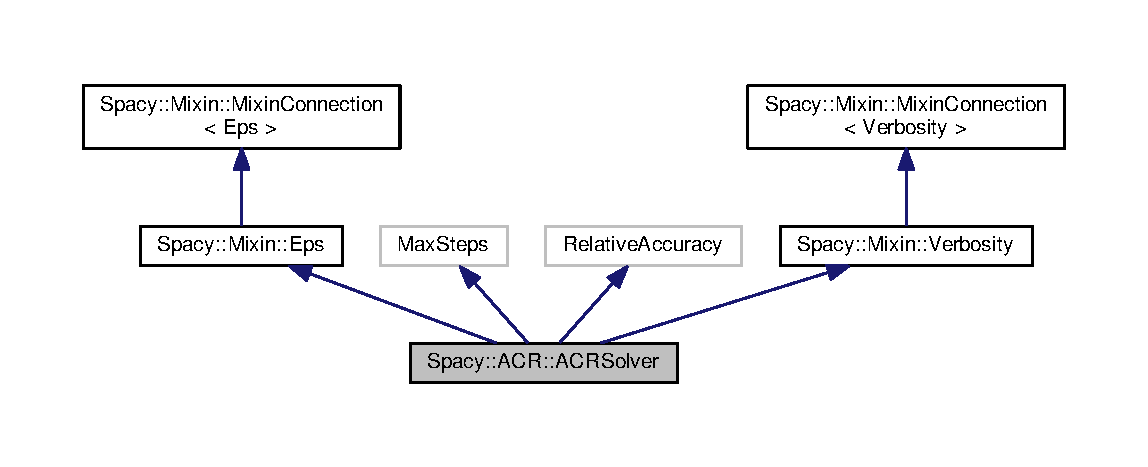
\includegraphics[width=350pt]{classSpacy_1_1ACR_1_1ACRSolver__inherit__graph}
\end{center}
\end{figure}


Collaboration diagram for Spacy\-:\-:A\-C\-R\-:\-:A\-C\-R\-Solver\-:
\nopagebreak
\begin{figure}[H]
\begin{center}
\leavevmode
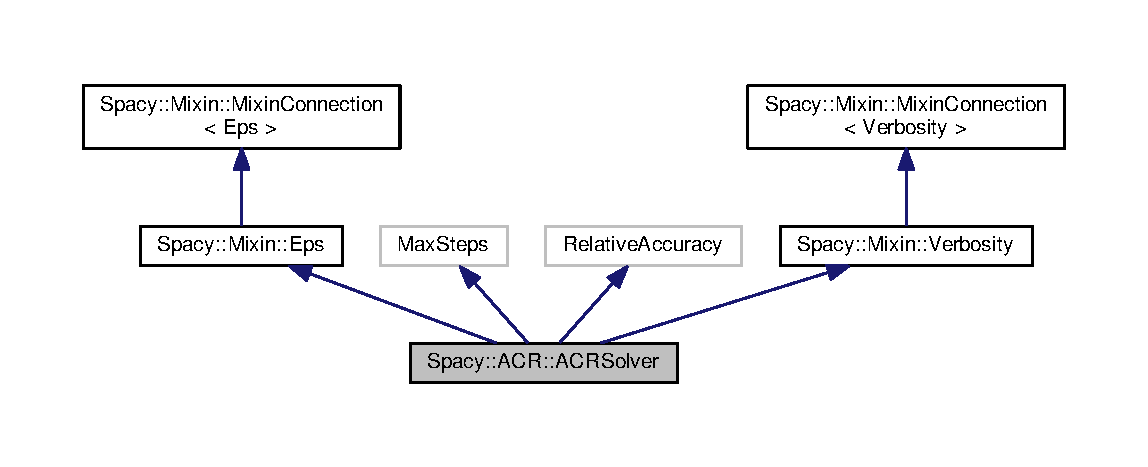
\includegraphics[width=350pt]{classSpacy_1_1ACR_1_1ACRSolver__coll__graph}
\end{center}
\end{figure}
\subsection*{Public Member Functions}
\begin{DoxyCompactItemize}
\item 
\hyperlink{classSpacy_1_1ACR_1_1ACRSolver_a2b442c8c3149e3d9ba866d9d60c8e014}{A\-C\-R\-Solver} (\hyperlink{classSpacy_1_1C2Functional}{C2\-Functional} f, double eta1=0.\-25, double eta2=0.\-5, double epsilon=1e-\/4, double relative\-Accuracy=1e-\/4, double omega\-Max=1e8, double lambda\-Max=2e-\/2)
\begin{DoxyCompactList}\small\item\em Constructor. \end{DoxyCompactList}\item 
\hypertarget{classSpacy_1_1ACR_1_1ACRSolver_ae68748adce75b5762ac7005024e29974}{\hyperlink{classSpacy_1_1Vector}{Vector} \hyperlink{classSpacy_1_1ACR_1_1ACRSolver_ae68748adce75b5762ac7005024e29974}{operator()} ()}\label{classSpacy_1_1ACR_1_1ACRSolver_ae68748adce75b5762ac7005024e29974}

\begin{DoxyCompactList}\small\item\em Compute solution starting at $x_0=0$. \end{DoxyCompactList}\item 
\hyperlink{classSpacy_1_1Vector}{Vector} \hyperlink{classSpacy_1_1ACR_1_1ACRSolver_ac7bc2ff6568728c4bd79f49f3596d2bc}{operator()} (const \hyperlink{classSpacy_1_1Vector}{Vector} \&x0)
\begin{DoxyCompactList}\small\item\em Compute solution. \end{DoxyCompactList}\item 
\hypertarget{classSpacy_1_1Mixin_1_1Eps_a818ab6dfab5e4eea583e1302bcc621f8}{void {\bfseries set\-\_\-eps} (\hyperlink{classSpacy_1_1Real}{Real} \hyperlink{classSpacy_1_1Mixin_1_1Eps_a812b99b0abc1d78a34b4114907f23f52}{eps})}\label{classSpacy_1_1Mixin_1_1Eps_a818ab6dfab5e4eea583e1302bcc621f8}

\item 
\hypertarget{classSpacy_1_1Mixin_1_1Eps_a812b99b0abc1d78a34b4114907f23f52}{\hyperlink{classSpacy_1_1Real}{Real} \hyperlink{classSpacy_1_1Mixin_1_1Eps_a812b99b0abc1d78a34b4114907f23f52}{eps} () const noexcept}\label{classSpacy_1_1Mixin_1_1Eps_a812b99b0abc1d78a34b4114907f23f52}

\begin{DoxyCompactList}\small\item\em Access $\varepsilon$. \end{DoxyCompactList}\item 
\hypertarget{classSpacy_1_1Mixin_1_1Eps_a1c1b0ed7f14ed4967dc7da9295a136d4}{\hyperlink{classSpacy_1_1Real}{Real} \hyperlink{classSpacy_1_1Mixin_1_1Eps_a1c1b0ed7f14ed4967dc7da9295a136d4}{sqrt\-\_\-eps} () const noexcept}\label{classSpacy_1_1Mixin_1_1Eps_a1c1b0ed7f14ed4967dc7da9295a136d4}

\begin{DoxyCompactList}\small\item\em Access $\sqrt\varepsilon$. \end{DoxyCompactList}\item 
\hypertarget{classSpacy_1_1Mixin_1_1Eps_a91dbe45e297be2bc53f1a96107a58c64}{\hyperlink{classSpacy_1_1Real}{Real} \hyperlink{classSpacy_1_1Mixin_1_1Eps_a91dbe45e297be2bc53f1a96107a58c64}{cbrt\-\_\-eps} () const noexcept}\label{classSpacy_1_1Mixin_1_1Eps_a91dbe45e297be2bc53f1a96107a58c64}

\begin{DoxyCompactList}\small\item\em Access $\varepsilon^{1/3}$. \end{DoxyCompactList}\item 
\hypertarget{classSpacy_1_1Mixin_1_1Eps_a151216968daef3da5f5cdc0b957ce01b}{void \hyperlink{classSpacy_1_1Mixin_1_1Eps_a151216968daef3da5f5cdc0b957ce01b}{update} (\hyperlink{classSpacy_1_1Mixin_1_1Eps_af616ae8e55a645cefd4d2d4504d6705a}{Eps} $\ast$changed\-Subject)}\label{classSpacy_1_1Mixin_1_1Eps_a151216968daef3da5f5cdc0b957ce01b}

\begin{DoxyCompactList}\small\item\em update function for observer pattern. \end{DoxyCompactList}\item 
\hypertarget{classSpacy_1_1Mixin_1_1MixinConnection_abb5520ee6b22dd993d78f142939a1ed4}{void \hyperlink{classSpacy_1_1Mixin_1_1MixinConnection_abb5520ee6b22dd993d78f142939a1ed4}{attach} (\hyperlink{classSpacy_1_1Mixin_1_1Eps_af616ae8e55a645cefd4d2d4504d6705a}{Eps} \&observer)}\label{classSpacy_1_1Mixin_1_1MixinConnection_abb5520ee6b22dd993d78f142939a1ed4}

\begin{DoxyCompactList}\small\item\em Attach observer. \end{DoxyCompactList}\item 
\hypertarget{classSpacy_1_1Mixin_1_1MixinConnection_adda739590c487679c26f60e50aedb73f}{void \hyperlink{classSpacy_1_1Mixin_1_1MixinConnection_adda739590c487679c26f60e50aedb73f}{detach} (\hyperlink{classSpacy_1_1Mixin_1_1Eps_af616ae8e55a645cefd4d2d4504d6705a}{Eps} \&observer)}\label{classSpacy_1_1Mixin_1_1MixinConnection_adda739590c487679c26f60e50aedb73f}

\begin{DoxyCompactList}\small\item\em Detach observer. \end{DoxyCompactList}\item 
\hypertarget{classSpacy_1_1Mixin_1_1MixinConnection_a1ddeaa78a3bb4a38c2cca36d1f99fe36}{void \hyperlink{classSpacy_1_1Mixin_1_1MixinConnection_a1ddeaa78a3bb4a38c2cca36d1f99fe36}{notify} ()}\label{classSpacy_1_1Mixin_1_1MixinConnection_a1ddeaa78a3bb4a38c2cca36d1f99fe36}

\begin{DoxyCompactList}\small\item\em Notify observers about changes. \end{DoxyCompactList}\item 
void \hyperlink{classSpacy_1_1Mixin_1_1Verbosity_a0365d293ab27e27da9496c668020aefb}{set\-Verbosity} (bool \hyperlink{classSpacy_1_1Mixin_1_1Verbosity_ad367a7328578546938fd2a7e52ab3793}{verbose})
\begin{DoxyCompactList}\small\item\em Enable/disable verbosity. \end{DoxyCompactList}\item 
\hypertarget{classSpacy_1_1Mixin_1_1Verbosity_ad367a7328578546938fd2a7e52ab3793}{bool \hyperlink{classSpacy_1_1Mixin_1_1Verbosity_ad367a7328578546938fd2a7e52ab3793}{verbose} () const noexcept}\label{classSpacy_1_1Mixin_1_1Verbosity_ad367a7328578546938fd2a7e52ab3793}

\begin{DoxyCompactList}\small\item\em Check if verbosity\-Level $>$ 0. \end{DoxyCompactList}\item 
\hypertarget{classSpacy_1_1Mixin_1_1Verbosity_af84a4b3c933f252a5840ab63d4a38325}{void {\bfseries set\-Verbosity\-Level} (unsigned level) noexcept}\label{classSpacy_1_1Mixin_1_1Verbosity_af84a4b3c933f252a5840ab63d4a38325}

\item 
\hypertarget{classSpacy_1_1Mixin_1_1Verbosity_ae55b7493c53b3bb4c2770c99addb5ee1}{unsigned \hyperlink{classSpacy_1_1Mixin_1_1Verbosity_ae55b7493c53b3bb4c2770c99addb5ee1}{get\-Verbosity\-Level} () const noexcept}\label{classSpacy_1_1Mixin_1_1Verbosity_ae55b7493c53b3bb4c2770c99addb5ee1}

\begin{DoxyCompactList}\small\item\em Access verbosity level. \end{DoxyCompactList}\item 
\hypertarget{classSpacy_1_1Mixin_1_1Verbosity_a8cff860c587fcda2cdc86ba744302b33}{void \hyperlink{classSpacy_1_1Mixin_1_1Verbosity_a8cff860c587fcda2cdc86ba744302b33}{update} (\hyperlink{classSpacy_1_1Mixin_1_1Verbosity_aefe2f237b0456c4bced001fbfa75f92e}{Verbosity} $\ast$changed\-Subject)}\label{classSpacy_1_1Mixin_1_1Verbosity_a8cff860c587fcda2cdc86ba744302b33}

\begin{DoxyCompactList}\small\item\em update function for observer pattern. \end{DoxyCompactList}\item 
\hypertarget{classSpacy_1_1Mixin_1_1MixinConnection_abb5520ee6b22dd993d78f142939a1ed4}{void \hyperlink{classSpacy_1_1Mixin_1_1MixinConnection_abb5520ee6b22dd993d78f142939a1ed4}{attach} (\hyperlink{classSpacy_1_1Mixin_1_1Verbosity_aefe2f237b0456c4bced001fbfa75f92e}{Verbosity} \&observer)}\label{classSpacy_1_1Mixin_1_1MixinConnection_abb5520ee6b22dd993d78f142939a1ed4}

\begin{DoxyCompactList}\small\item\em Attach observer. \end{DoxyCompactList}\item 
\hypertarget{classSpacy_1_1Mixin_1_1MixinConnection_adda739590c487679c26f60e50aedb73f}{void \hyperlink{classSpacy_1_1Mixin_1_1MixinConnection_adda739590c487679c26f60e50aedb73f}{detach} (\hyperlink{classSpacy_1_1Mixin_1_1Verbosity_aefe2f237b0456c4bced001fbfa75f92e}{Verbosity} \&observer)}\label{classSpacy_1_1Mixin_1_1MixinConnection_adda739590c487679c26f60e50aedb73f}

\begin{DoxyCompactList}\small\item\em Detach observer. \end{DoxyCompactList}\item 
\hypertarget{classSpacy_1_1Mixin_1_1MixinConnection_a1ddeaa78a3bb4a38c2cca36d1f99fe36}{void \hyperlink{classSpacy_1_1Mixin_1_1MixinConnection_a1ddeaa78a3bb4a38c2cca36d1f99fe36}{notify} ()}\label{classSpacy_1_1Mixin_1_1MixinConnection_a1ddeaa78a3bb4a38c2cca36d1f99fe36}

\begin{DoxyCompactList}\small\item\em Notify observers about changes. \end{DoxyCompactList}\end{DoxyCompactItemize}


\subsection{Detailed Description}
Adaptive cubic regularization approach for solving unconstrained minimization problems Compute direction of descent with one \hyperlink{namespaceSpacy_1_1Newton}{Newton} step Use a cubic error model to obtain acceptable corrections Solve problems of the form \[\min f(x).\]. 

\subsection{Constructor \& Destructor Documentation}
\hypertarget{classSpacy_1_1ACR_1_1ACRSolver_a2b442c8c3149e3d9ba866d9d60c8e014}{\index{Spacy\-::\-A\-C\-R\-::\-A\-C\-R\-Solver@{Spacy\-::\-A\-C\-R\-::\-A\-C\-R\-Solver}!A\-C\-R\-Solver@{A\-C\-R\-Solver}}
\index{A\-C\-R\-Solver@{A\-C\-R\-Solver}!Spacy::ACR::ACRSolver@{Spacy\-::\-A\-C\-R\-::\-A\-C\-R\-Solver}}
\subsubsection[{A\-C\-R\-Solver}]{\setlength{\rightskip}{0pt plus 5cm}Spacy\-::\-A\-C\-R\-::\-A\-C\-R\-Solver\-::\-A\-C\-R\-Solver (
\begin{DoxyParamCaption}
\item[{{\bf C2\-Functional}}]{f, }
\item[{double}]{eta1 = {\ttfamily 0.25}, }
\item[{double}]{eta2 = {\ttfamily 0.5}, }
\item[{double}]{epsilon = {\ttfamily 1e-\/4}, }
\item[{double}]{relative\-Accuracy = {\ttfamily 1e-\/4}, }
\item[{double}]{omega\-Max = {\ttfamily 1e8}, }
\item[{double}]{lambda\-Max = {\ttfamily 2e-\/2}}
\end{DoxyParamCaption}
)}}\label{classSpacy_1_1ACR_1_1ACRSolver_a2b442c8c3149e3d9ba866d9d60c8e014}


Constructor. 


\begin{DoxyParams}{Parameters}
{\em f} & functional to minimize \\
\hline
\end{DoxyParams}


\subsection{Member Function Documentation}
\hypertarget{classSpacy_1_1ACR_1_1ACRSolver_ac7bc2ff6568728c4bd79f49f3596d2bc}{\index{Spacy\-::\-A\-C\-R\-::\-A\-C\-R\-Solver@{Spacy\-::\-A\-C\-R\-::\-A\-C\-R\-Solver}!operator()@{operator()}}
\index{operator()@{operator()}!Spacy::ACR::ACRSolver@{Spacy\-::\-A\-C\-R\-::\-A\-C\-R\-Solver}}
\subsubsection[{operator()}]{\setlength{\rightskip}{0pt plus 5cm}{\bf Vector} Spacy\-::\-A\-C\-R\-::\-A\-C\-R\-Solver\-::operator() (
\begin{DoxyParamCaption}
\item[{const {\bf Vector} \&}]{x0}
\end{DoxyParamCaption}
)}}\label{classSpacy_1_1ACR_1_1ACRSolver_ac7bc2ff6568728c4bd79f49f3596d2bc}


Compute solution. 


\begin{DoxyParams}{Parameters}
{\em x0} & initial iterate \\
\hline
\end{DoxyParams}
\hypertarget{classSpacy_1_1Mixin_1_1Verbosity_a0365d293ab27e27da9496c668020aefb}{\index{Spacy\-::\-A\-C\-R\-::\-A\-C\-R\-Solver@{Spacy\-::\-A\-C\-R\-::\-A\-C\-R\-Solver}!set\-Verbosity@{set\-Verbosity}}
\index{set\-Verbosity@{set\-Verbosity}!Spacy::ACR::ACRSolver@{Spacy\-::\-A\-C\-R\-::\-A\-C\-R\-Solver}}
\subsubsection[{set\-Verbosity}]{\setlength{\rightskip}{0pt plus 5cm}void Spacy\-::\-Mixin\-::\-Verbosity\-::set\-Verbosity (
\begin{DoxyParamCaption}
\item[{bool}]{verbose}
\end{DoxyParamCaption}
)\hspace{0.3cm}{\ttfamily [inherited]}}}\label{classSpacy_1_1Mixin_1_1Verbosity_a0365d293ab27e27da9496c668020aefb}


Enable/disable verbosity. 


\begin{DoxyParams}{Parameters}
{\em verbose} & true\-: if verbosity\-Level = 0, set verbosity\-Level = 1; false\-: if set verbosity\-Level = 0 \\
\hline
\end{DoxyParams}


The documentation for this class was generated from the following file\-:\begin{DoxyCompactItemize}
\item 
/home/travis/build/spacy-\/dev/\-Spacy/\-Spacy/\-Algorithm/\-A\-C\-R/acr.\-hh\end{DoxyCompactItemize}

\hypertarget{classSpacy_1_1AdaptiveInducedScalarProduct}{}\section{Spacy\+:\+:Adaptive\+Induced\+Scalar\+Product Class Reference}
\label{classSpacy_1_1AdaptiveInducedScalarProduct}\index{Spacy\+::\+Adaptive\+Induced\+Scalar\+Product@{Spacy\+::\+Adaptive\+Induced\+Scalar\+Product}}


Induced scalar product $(x,y)_M = (Mx)y$, where $M:X\rightarrow X^*$.  




{\ttfamily \#include $<$induced\+Scalar\+Product.\+hh$>$}

\subsection*{Public Member Functions}
\begin{DoxyCompactItemize}
\item 
\hyperlink{classSpacy_1_1AdaptiveInducedScalarProduct_ae96382f8f7287b0f64176932196bca1b}{Adaptive\+Induced\+Scalar\+Product} (std\+::function$<$ \hyperlink{classSpacy_1_1LinearOperator}{Linear\+Operator}()$>$ operator\+Creator)
\begin{DoxyCompactList}\small\item\em Constructor. \end{DoxyCompactList}\item 
\hyperlink{classSpacy_1_1Real}{Real} \hyperlink{classSpacy_1_1AdaptiveInducedScalarProduct_a0909b9825f324aa3427b41a87abd395d}{operator()} (const \hyperlink{classSpacy_1_1Vector}{Vector} \&x, const \hyperlink{classSpacy_1_1Vector}{Vector} \&y) const \hypertarget{classSpacy_1_1AdaptiveInducedScalarProduct_a0909b9825f324aa3427b41a87abd395d}{}\label{classSpacy_1_1AdaptiveInducedScalarProduct_a0909b9825f324aa3427b41a87abd395d}

\begin{DoxyCompactList}\small\item\em Compute scalar product $(x,y)_M$. \end{DoxyCompactList}\end{DoxyCompactItemize}


\subsection{Detailed Description}
Induced scalar product $(x,y)_M = (Mx)y$, where $M:X\rightarrow X^*$. 

\subsection{Constructor \& Destructor Documentation}
\index{Spacy\+::\+Adaptive\+Induced\+Scalar\+Product@{Spacy\+::\+Adaptive\+Induced\+Scalar\+Product}!Adaptive\+Induced\+Scalar\+Product@{Adaptive\+Induced\+Scalar\+Product}}
\index{Adaptive\+Induced\+Scalar\+Product@{Adaptive\+Induced\+Scalar\+Product}!Spacy\+::\+Adaptive\+Induced\+Scalar\+Product@{Spacy\+::\+Adaptive\+Induced\+Scalar\+Product}}
\subsubsection[{\texorpdfstring{Adaptive\+Induced\+Scalar\+Product(std\+::function$<$ Linear\+Operator()$>$ operator\+Creator)}{AdaptiveInducedScalarProduct(std::function< LinearOperator()> operatorCreator)}}]{\setlength{\rightskip}{0pt plus 5cm}Spacy\+::\+Adaptive\+Induced\+Scalar\+Product\+::\+Adaptive\+Induced\+Scalar\+Product (
\begin{DoxyParamCaption}
\item[{std\+::function$<$ {\bf Linear\+Operator}()$>$}]{operator\+Creator}
\end{DoxyParamCaption}
)\hspace{0.3cm}{\ttfamily [explicit]}}\hypertarget{classSpacy_1_1AdaptiveInducedScalarProduct_ae96382f8f7287b0f64176932196bca1b}{}\label{classSpacy_1_1AdaptiveInducedScalarProduct_ae96382f8f7287b0f64176932196bca1b}


Constructor. 


\begin{DoxyParams}{Parameters}
{\em M} & operator defining the scalar product. \\
\hline
\end{DoxyParams}


The documentation for this class was generated from the following file\+:\begin{DoxyCompactItemize}
\item 
/home/lars/tmp/\+Spacy/\+Spacy/induced\+Scalar\+Product.\+hh\end{DoxyCompactItemize}

\hypertarget{classSpacy_1_1AddArithmeticOperators}{\section{\-Spacy\-:\-:\-Add\-Arithmetic\-Operators$<$ \-Derived $>$ \-Class \-Template \-Reference}
\label{classSpacy_1_1AddArithmeticOperators}\index{\-Spacy\-::\-Add\-Arithmetic\-Operators$<$ Derived $>$@{\-Spacy\-::\-Add\-Arithmetic\-Operators$<$ Derived $>$}}
}


\-Base class providing some operations for vectors via \-C\-R\-T\-P.  




{\ttfamily \#include $<$\-Add\-Arithmetic\-Operators.\-hh$>$}

\subsection*{\-Public \-Member \-Functions}
\begin{DoxyCompactItemize}
\item 
\-Derived \& \hyperlink{classSpacy_1_1AddArithmeticOperators_afad1d01e1e8c6f75290ac46d9b047ea8}{operator+=} (const \-Derived \&y)
\begin{DoxyCompactList}\small\item\em \-In-\/place summation $ x+=y$. \end{DoxyCompactList}\item 
\-Derived \& \hyperlink{classSpacy_1_1AddArithmeticOperators_a9fa91e177d13203cfe8cfa991c64ca36}{operator-\/=} (const \-Derived \&y)
\begin{DoxyCompactList}\small\item\em \-In-\/place subtraction $ x-=y$. \end{DoxyCompactList}\item 
\-Derived \& \hyperlink{classSpacy_1_1AddArithmeticOperators_a1d3db95b24fd2bc1de712c9e04c47e2f}{operator$\ast$=} (double a)
\begin{DoxyCompactList}\small\item\em \-In-\/place multiplication $ x*=a$. \end{DoxyCompactList}\item 
\-Derived \hyperlink{classSpacy_1_1AddArithmeticOperators_a5acd030bf265d130983fd6e3c5b68be5}{operator-\/} () const 
\begin{DoxyCompactList}\small\item\em \-Negation $ -x$. \end{DoxyCompactList}\item 
bool \hyperlink{classSpacy_1_1AddArithmeticOperators_a5ff1909f49f4a705d69663dc2d4b6316}{operator==} (const \-Derived \&y) const 
\begin{DoxyCompactList}\small\item\em \-Comparison operator $ x==y$. \end{DoxyCompactList}\end{DoxyCompactItemize}


\subsection{\-Detailed \-Description}
\subsubsection*{template$<$class \-Derived$>$class Spacy\-::\-Add\-Arithmetic\-Operators$<$ Derived $>$}

\-Base class providing some operations for vectors via \-C\-R\-T\-P. 


\begin{DoxyTemplParams}{\-Template Parameters}
{\em \-Derived} & derived vector implementation, provided for \-C\-R\-T\-P\\
\hline
\end{DoxyTemplParams}
\-Provides operator+=, operator-\/=, operator$\ast$=, operator-\/, operator==.

\begin{DoxySeeAlso}{\-See also}
\-Real\-::\-Vector, \-Fenics\-::\-Vector, \hyperlink{classSpacy_1_1Kaskade_1_1Vector}{\-Kaskade\-::\-Vector} 
\end{DoxySeeAlso}


\subsection{\-Member \-Function \-Documentation}
\hypertarget{classSpacy_1_1AddArithmeticOperators_afad1d01e1e8c6f75290ac46d9b047ea8}{\index{\-Spacy\-::\-Add\-Arithmetic\-Operators@{\-Spacy\-::\-Add\-Arithmetic\-Operators}!operator+=@{operator+=}}
\index{operator+=@{operator+=}!Spacy::AddArithmeticOperators@{\-Spacy\-::\-Add\-Arithmetic\-Operators}}
\subsubsection[{operator+=}]{\setlength{\rightskip}{0pt plus 5cm}template$<$class \-Derived$>$ \-Derived\& {\bf \-Spacy\-::\-Add\-Arithmetic\-Operators}$<$ \-Derived $>$\-::operator+= (
\begin{DoxyParamCaption}
\item[{const \-Derived \&}]{y}
\end{DoxyParamCaption}
)\hspace{0.3cm}{\ttfamily  \mbox{[}inline\mbox{]}}}}\label{classSpacy_1_1AddArithmeticOperators_afad1d01e1e8c6f75290ac46d9b047ea8}


\-In-\/place summation $ x+=y$. 


\begin{DoxyParams}{\-Parameters}
{\em y} & vector to add to this vector \\
\hline
\end{DoxyParams}
\begin{DoxyReturn}{\-Returns}
$ x+=y$. 
\end{DoxyReturn}
\hypertarget{classSpacy_1_1AddArithmeticOperators_a9fa91e177d13203cfe8cfa991c64ca36}{\index{\-Spacy\-::\-Add\-Arithmetic\-Operators@{\-Spacy\-::\-Add\-Arithmetic\-Operators}!operator-\/=@{operator-\/=}}
\index{operator-\/=@{operator-\/=}!Spacy::AddArithmeticOperators@{\-Spacy\-::\-Add\-Arithmetic\-Operators}}
\subsubsection[{operator-\/=}]{\setlength{\rightskip}{0pt plus 5cm}template$<$class \-Derived$>$ \-Derived\& {\bf \-Spacy\-::\-Add\-Arithmetic\-Operators}$<$ \-Derived $>$\-::operator-\/= (
\begin{DoxyParamCaption}
\item[{const \-Derived \&}]{y}
\end{DoxyParamCaption}
)\hspace{0.3cm}{\ttfamily  \mbox{[}inline\mbox{]}}}}\label{classSpacy_1_1AddArithmeticOperators_a9fa91e177d13203cfe8cfa991c64ca36}


\-In-\/place subtraction $ x-=y$. 


\begin{DoxyParams}{\-Parameters}
{\em y} & vector to subtract from this vector \\
\hline
\end{DoxyParams}
\begin{DoxyReturn}{\-Returns}
$ x-=y$. 
\end{DoxyReturn}
\hypertarget{classSpacy_1_1AddArithmeticOperators_a1d3db95b24fd2bc1de712c9e04c47e2f}{\index{\-Spacy\-::\-Add\-Arithmetic\-Operators@{\-Spacy\-::\-Add\-Arithmetic\-Operators}!operator$\ast$=@{operator$\ast$=}}
\index{operator$\ast$=@{operator$\ast$=}!Spacy::AddArithmeticOperators@{\-Spacy\-::\-Add\-Arithmetic\-Operators}}
\subsubsection[{operator$\ast$=}]{\setlength{\rightskip}{0pt plus 5cm}template$<$class \-Derived$>$ \-Derived\& {\bf \-Spacy\-::\-Add\-Arithmetic\-Operators}$<$ \-Derived $>$\-::operator$\ast$= (
\begin{DoxyParamCaption}
\item[{double}]{a}
\end{DoxyParamCaption}
)\hspace{0.3cm}{\ttfamily  \mbox{[}inline\mbox{]}}}}\label{classSpacy_1_1AddArithmeticOperators_a1d3db95b24fd2bc1de712c9e04c47e2f}


\-In-\/place multiplication $ x*=a$. 


\begin{DoxyParams}{\-Parameters}
{\em a} & scaling factor \\
\hline
\end{DoxyParams}
\begin{DoxyReturn}{\-Returns}
$ x*=a$. 
\end{DoxyReturn}
\hypertarget{classSpacy_1_1AddArithmeticOperators_a5acd030bf265d130983fd6e3c5b68be5}{\index{\-Spacy\-::\-Add\-Arithmetic\-Operators@{\-Spacy\-::\-Add\-Arithmetic\-Operators}!operator-\/@{operator-\/}}
\index{operator-\/@{operator-\/}!Spacy::AddArithmeticOperators@{\-Spacy\-::\-Add\-Arithmetic\-Operators}}
\subsubsection[{operator-\/}]{\setlength{\rightskip}{0pt plus 5cm}template$<$class \-Derived$>$ \-Derived {\bf \-Spacy\-::\-Add\-Arithmetic\-Operators}$<$ \-Derived $>$\-::operator-\/ (
\begin{DoxyParamCaption}
{}
\end{DoxyParamCaption}
) const\hspace{0.3cm}{\ttfamily  \mbox{[}inline\mbox{]}}}}\label{classSpacy_1_1AddArithmeticOperators_a5acd030bf265d130983fd6e3c5b68be5}


\-Negation $ -x$. 

\begin{DoxyReturn}{\-Returns}
$ -x $. 
\end{DoxyReturn}


\-Reimplemented in \hyperlink{structSpacy_1_1Scalar_1_1LinearOperator_aba7eb546eca4983adcf2e39155af07d1}{\-Spacy\-::\-Scalar\-::\-Linear\-Operator}.

\hypertarget{classSpacy_1_1AddArithmeticOperators_a5ff1909f49f4a705d69663dc2d4b6316}{\index{\-Spacy\-::\-Add\-Arithmetic\-Operators@{\-Spacy\-::\-Add\-Arithmetic\-Operators}!operator==@{operator==}}
\index{operator==@{operator==}!Spacy::AddArithmeticOperators@{\-Spacy\-::\-Add\-Arithmetic\-Operators}}
\subsubsection[{operator==}]{\setlength{\rightskip}{0pt plus 5cm}template$<$class \-Derived$>$ bool {\bf \-Spacy\-::\-Add\-Arithmetic\-Operators}$<$ \-Derived $>$\-::operator== (
\begin{DoxyParamCaption}
\item[{const \-Derived \&}]{y}
\end{DoxyParamCaption}
) const\hspace{0.3cm}{\ttfamily  \mbox{[}inline\mbox{]}}}}\label{classSpacy_1_1AddArithmeticOperators_a5ff1909f49f4a705d69663dc2d4b6316}


\-Comparison operator $ x==y$. 


\begin{DoxyParams}{\-Parameters}
{\em y} & vector to compare with this vector \\
\hline
\end{DoxyParams}
\begin{DoxyReturn}{\-Returns}
$ x==y$. 
\end{DoxyReturn}


\-The documentation for this class was generated from the following file\-:\begin{DoxyCompactItemize}
\item 
/home/travis/build/spacy-\/dev/\-Spacy/\-Spacy/\-Util/\-Base/\-Add\-Arithmetic\-Operators.\-hh\end{DoxyCompactItemize}

\hypertarget{classSpacy_1_1Newton_1_1Damping_1_1AffineContravariant}{\section{\-Spacy\-:\-:\-Newton\-:\-:\-Damping\-:\-:\-Affine\-Contravariant \-Class \-Reference}
\label{classSpacy_1_1Newton_1_1Damping_1_1AffineContravariant}\index{\-Spacy\-::\-Newton\-::\-Damping\-::\-Affine\-Contravariant@{\-Spacy\-::\-Newton\-::\-Damping\-::\-Affine\-Contravariant}}
}


\-Affine contravariant damping strategy as described in.  




{\ttfamily \#include $<$damping\-Strategies.\-hh$>$}



\-Inheritance diagram for \-Spacy\-:\-:\-Newton\-:\-:\-Damping\-:\-:\-Affine\-Contravariant\-:
\nopagebreak
\begin{figure}[H]
\begin{center}
\leavevmode
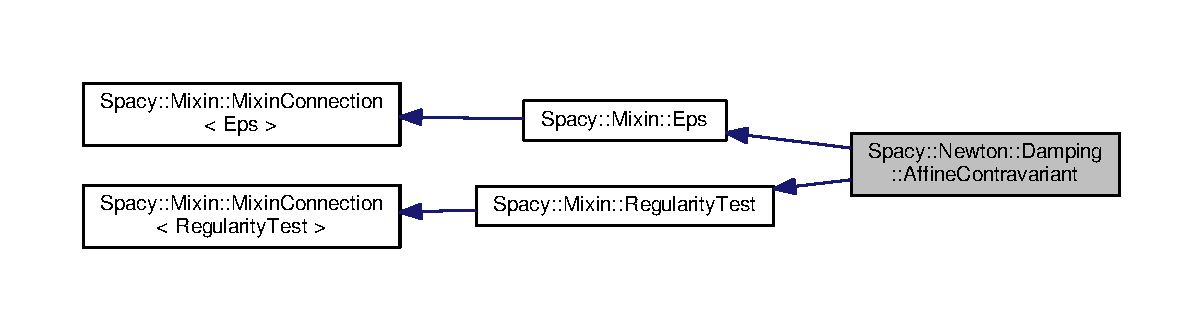
\includegraphics[width=350pt]{classSpacy_1_1Newton_1_1Damping_1_1AffineContravariant__inherit__graph}
\end{center}
\end{figure}


\-Collaboration diagram for \-Spacy\-:\-:\-Newton\-:\-:\-Damping\-:\-:\-Affine\-Contravariant\-:
\nopagebreak
\begin{figure}[H]
\begin{center}
\leavevmode
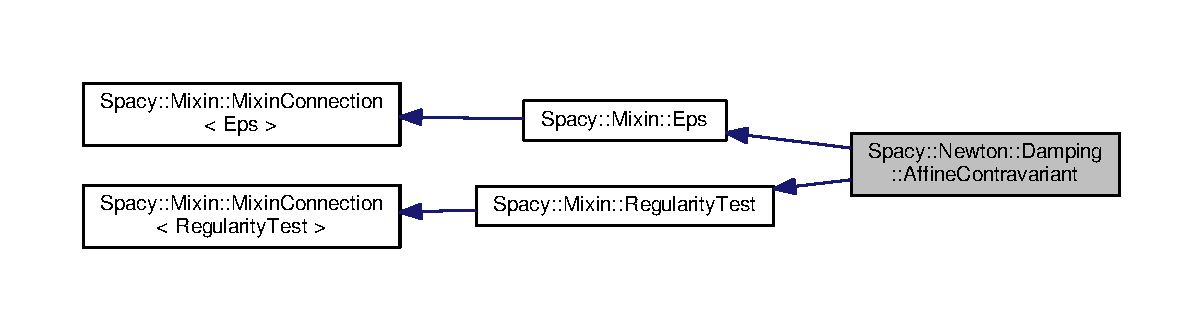
\includegraphics[width=350pt]{classSpacy_1_1Newton_1_1Damping_1_1AffineContravariant__coll__graph}
\end{center}
\end{figure}
\subsection*{\-Public \-Member \-Functions}
\begin{DoxyCompactItemize}
\item 
\hypertarget{classSpacy_1_1Newton_1_1Damping_1_1AffineContravariant_afbb2954f22af6d8248ec9c382a5b1ccd}{\hyperlink{classSpacy_1_1Newton_1_1Damping_1_1AffineContravariant_afbb2954f22af6d8248ec9c382a5b1ccd}{\-Affine\-Contravariant} (const \hyperlink{classSpacy_1_1C1Operator}{\-C1\-Operator} \&\-F)}\label{classSpacy_1_1Newton_1_1Damping_1_1AffineContravariant_afbb2954f22af6d8248ec9c382a5b1ccd}

\begin{DoxyCompactList}\small\item\em \-Constructor. \end{DoxyCompactList}\item 
\hypertarget{classSpacy_1_1Newton_1_1Damping_1_1AffineContravariant_a494dcf0e1c7837b4b6bd18107efcfe0b}{\hyperlink{classSpacy_1_1DampingFactor}{\-Damping\-Factor} \hyperlink{classSpacy_1_1Newton_1_1Damping_1_1AffineContravariant_a494dcf0e1c7837b4b6bd18107efcfe0b}{operator()} (const std\-::function$<$ \hyperlink{classSpacy_1_1Vector}{\-Vector}(const \hyperlink{classSpacy_1_1Vector}{\-Vector} \&)$>$ \&, const \hyperlink{classSpacy_1_1Vector}{\-Vector} \&x, const \hyperlink{classSpacy_1_1Vector}{\-Vector} \&dx) const }\label{classSpacy_1_1Newton_1_1Damping_1_1AffineContravariant_a494dcf0e1c7837b4b6bd18107efcfe0b}

\begin{DoxyCompactList}\small\item\em \-Compute damping factor. \end{DoxyCompactList}\item 
\hypertarget{classSpacy_1_1Mixin_1_1Eps_a6b4c38a60848c0ab665fb3a81e181786}{void {\bfseries set\-Eps} (\hyperlink{classSpacy_1_1Real}{\-Real} \hyperlink{classSpacy_1_1Mixin_1_1Eps_a812b99b0abc1d78a34b4114907f23f52}{eps})}\label{classSpacy_1_1Mixin_1_1Eps_a6b4c38a60848c0ab665fb3a81e181786}

\item 
\hypertarget{classSpacy_1_1Mixin_1_1Eps_a812b99b0abc1d78a34b4114907f23f52}{\hyperlink{classSpacy_1_1Real}{\-Real} \hyperlink{classSpacy_1_1Mixin_1_1Eps_a812b99b0abc1d78a34b4114907f23f52}{eps} () const noexcept}\label{classSpacy_1_1Mixin_1_1Eps_a812b99b0abc1d78a34b4114907f23f52}

\begin{DoxyCompactList}\small\item\em \-Access $\varepsilon$. \end{DoxyCompactList}\item 
\hypertarget{classSpacy_1_1Mixin_1_1Eps_abd50a47b32614a950189855775a09d05}{\hyperlink{classSpacy_1_1Real}{\-Real} \hyperlink{classSpacy_1_1Mixin_1_1Eps_abd50a47b32614a950189855775a09d05}{sqrt\-Eps} () const noexcept}\label{classSpacy_1_1Mixin_1_1Eps_abd50a47b32614a950189855775a09d05}

\begin{DoxyCompactList}\small\item\em \-Access $\sqrt\varepsilon$. \end{DoxyCompactList}\item 
\hypertarget{classSpacy_1_1Mixin_1_1Eps_a4bbca3a4afc878d1a20b6335f35e58f7}{\hyperlink{classSpacy_1_1Real}{\-Real} \hyperlink{classSpacy_1_1Mixin_1_1Eps_a4bbca3a4afc878d1a20b6335f35e58f7}{cbrt\-Eps} () const noexcept}\label{classSpacy_1_1Mixin_1_1Eps_a4bbca3a4afc878d1a20b6335f35e58f7}

\begin{DoxyCompactList}\small\item\em \-Access $\varepsilon^{1/3}$. \end{DoxyCompactList}\item 
\hypertarget{classSpacy_1_1Mixin_1_1Eps_a151216968daef3da5f5cdc0b957ce01b}{void \hyperlink{classSpacy_1_1Mixin_1_1Eps_a151216968daef3da5f5cdc0b957ce01b}{update} (\hyperlink{classSpacy_1_1Mixin_1_1Eps_af616ae8e55a645cefd4d2d4504d6705a}{\-Eps} $\ast$changed\-Subject)}\label{classSpacy_1_1Mixin_1_1Eps_a151216968daef3da5f5cdc0b957ce01b}

\begin{DoxyCompactList}\small\item\em update function for observer pattern. \end{DoxyCompactList}\item 
\hypertarget{classSpacy_1_1Mixin_1_1MixinConnection_abb5520ee6b22dd993d78f142939a1ed4}{void \hyperlink{classSpacy_1_1Mixin_1_1MixinConnection_abb5520ee6b22dd993d78f142939a1ed4}{attach} (\hyperlink{classSpacy_1_1Mixin_1_1Eps_af616ae8e55a645cefd4d2d4504d6705a}{\-Eps} \&observer)}\label{classSpacy_1_1Mixin_1_1MixinConnection_abb5520ee6b22dd993d78f142939a1ed4}

\begin{DoxyCompactList}\small\item\em \-Attach observer. \end{DoxyCompactList}\item 
\hypertarget{classSpacy_1_1Mixin_1_1MixinConnection_adda739590c487679c26f60e50aedb73f}{void \hyperlink{classSpacy_1_1Mixin_1_1MixinConnection_adda739590c487679c26f60e50aedb73f}{detach} (\hyperlink{classSpacy_1_1Mixin_1_1Eps_af616ae8e55a645cefd4d2d4504d6705a}{\-Eps} \&observer)}\label{classSpacy_1_1Mixin_1_1MixinConnection_adda739590c487679c26f60e50aedb73f}

\begin{DoxyCompactList}\small\item\em \-Detach observer. \end{DoxyCompactList}\item 
\hypertarget{classSpacy_1_1Mixin_1_1MixinConnection_a1ddeaa78a3bb4a38c2cca36d1f99fe36}{void \hyperlink{classSpacy_1_1Mixin_1_1MixinConnection_a1ddeaa78a3bb4a38c2cca36d1f99fe36}{notify} ()}\label{classSpacy_1_1Mixin_1_1MixinConnection_a1ddeaa78a3bb4a38c2cca36d1f99fe36}

\begin{DoxyCompactList}\small\item\em \-Notify observers about changes. \end{DoxyCompactList}\item 
\hypertarget{classSpacy_1_1Mixin_1_1RegularityTest_a682ce022b0b5493e48f50f693ed64082}{void \hyperlink{classSpacy_1_1Mixin_1_1RegularityTest_a682ce022b0b5493e48f50f693ed64082}{set\-Lower\-Bound} (\hyperlink{classSpacy_1_1DampingFactor}{\-Damping\-Factor} lower\-Bound)}\label{classSpacy_1_1Mixin_1_1RegularityTest_a682ce022b0b5493e48f50f693ed64082}

\begin{DoxyCompactList}\small\item\em \-Set lower bound of regularity test for termination criteria. \end{DoxyCompactList}\item 
\hypertarget{classSpacy_1_1Mixin_1_1RegularityTest_a576995201badbfaee2064bf0d7749257}{\hyperlink{classSpacy_1_1DampingFactor}{\-Damping\-Factor} {\bfseries get\-Lower\-Bound} () const noexcept}\label{classSpacy_1_1Mixin_1_1RegularityTest_a576995201badbfaee2064bf0d7749257}

\item 
bool \hyperlink{classSpacy_1_1Mixin_1_1RegularityTest_acb6b3e8c76ebdbded0ec610959513caf}{regularity\-Test\-Passed} (\hyperlink{classSpacy_1_1DampingFactor}{\-Damping\-Factor} nu) const noexcept
\begin{DoxyCompactList}\small\item\em \-Apply regularity test. \end{DoxyCompactList}\item 
bool \hyperlink{classSpacy_1_1Mixin_1_1RegularityTest_aeb1a3b051bafc9da9be1df354c652812}{regularity\-Test\-Failed} (\hyperlink{classSpacy_1_1DampingFactor}{\-Damping\-Factor} nu) const noexcept
\begin{DoxyCompactList}\small\item\em \-Apply regularity test. \end{DoxyCompactList}\item 
\hypertarget{classSpacy_1_1Mixin_1_1RegularityTest_a1a6191e20f84025cec8b10ec63ab94ac}{void \hyperlink{classSpacy_1_1Mixin_1_1RegularityTest_a1a6191e20f84025cec8b10ec63ab94ac}{update} (\hyperlink{classSpacy_1_1Mixin_1_1RegularityTest_a548d9d45c31c7833266bd3b20dc1aa7e}{\-Regularity\-Test} $\ast$changed\-Subject)}\label{classSpacy_1_1Mixin_1_1RegularityTest_a1a6191e20f84025cec8b10ec63ab94ac}

\begin{DoxyCompactList}\small\item\em update function for observer pattern. \end{DoxyCompactList}\item 
\hypertarget{classSpacy_1_1Mixin_1_1MixinConnection_abb5520ee6b22dd993d78f142939a1ed4}{void \hyperlink{classSpacy_1_1Mixin_1_1MixinConnection_abb5520ee6b22dd993d78f142939a1ed4}{attach} (\hyperlink{classSpacy_1_1Mixin_1_1RegularityTest_a548d9d45c31c7833266bd3b20dc1aa7e}{\-Regularity\-Test} \&observer)}\label{classSpacy_1_1Mixin_1_1MixinConnection_abb5520ee6b22dd993d78f142939a1ed4}

\begin{DoxyCompactList}\small\item\em \-Attach observer. \end{DoxyCompactList}\item 
\hypertarget{classSpacy_1_1Mixin_1_1MixinConnection_adda739590c487679c26f60e50aedb73f}{void \hyperlink{classSpacy_1_1Mixin_1_1MixinConnection_adda739590c487679c26f60e50aedb73f}{detach} (\hyperlink{classSpacy_1_1Mixin_1_1RegularityTest_a548d9d45c31c7833266bd3b20dc1aa7e}{\-Regularity\-Test} \&observer)}\label{classSpacy_1_1Mixin_1_1MixinConnection_adda739590c487679c26f60e50aedb73f}

\begin{DoxyCompactList}\small\item\em \-Detach observer. \end{DoxyCompactList}\item 
\hypertarget{classSpacy_1_1Mixin_1_1MixinConnection_a1ddeaa78a3bb4a38c2cca36d1f99fe36}{void \hyperlink{classSpacy_1_1Mixin_1_1MixinConnection_a1ddeaa78a3bb4a38c2cca36d1f99fe36}{notify} ()}\label{classSpacy_1_1Mixin_1_1MixinConnection_a1ddeaa78a3bb4a38c2cca36d1f99fe36}

\begin{DoxyCompactList}\small\item\em \-Notify observers about changes. \end{DoxyCompactList}\end{DoxyCompactItemize}


\subsection{\-Detailed \-Description}
\-Affine contravariant damping strategy as described in. 

\cite{Deuflhard2004} \mbox{[}\-Sec. 3.\-2\mbox{]}. 

\subsection{\-Member \-Function \-Documentation}
\hypertarget{classSpacy_1_1Mixin_1_1RegularityTest_acb6b3e8c76ebdbded0ec610959513caf}{\index{\-Spacy\-::\-Newton\-::\-Damping\-::\-Affine\-Contravariant@{\-Spacy\-::\-Newton\-::\-Damping\-::\-Affine\-Contravariant}!regularity\-Test\-Passed@{regularity\-Test\-Passed}}
\index{regularity\-Test\-Passed@{regularity\-Test\-Passed}!Spacy::Newton::Damping::AffineContravariant@{\-Spacy\-::\-Newton\-::\-Damping\-::\-Affine\-Contravariant}}
\subsubsection[{regularity\-Test\-Passed}]{\setlength{\rightskip}{0pt plus 5cm}bool {\bf \-Spacy\-::\-Mixin\-::\-Regularity\-Test\-::regularity\-Test\-Passed} (
\begin{DoxyParamCaption}
\item[{{\bf \-Damping\-Factor}}]{nu}
\end{DoxyParamCaption}
) const\hspace{0.3cm}{\ttfamily  \mbox{[}inherited\mbox{]}}}}\label{classSpacy_1_1Mixin_1_1RegularityTest_acb6b3e8c76ebdbded0ec610959513caf}


\-Apply regularity test. 


\begin{DoxyParams}{\-Parameters}
{\em nu} & damping factor \\
\hline
\end{DoxyParams}
\begin{DoxyReturn}{\-Returns}
$nu > lowerBound_$ 
\end{DoxyReturn}
\hypertarget{classSpacy_1_1Mixin_1_1RegularityTest_aeb1a3b051bafc9da9be1df354c652812}{\index{\-Spacy\-::\-Newton\-::\-Damping\-::\-Affine\-Contravariant@{\-Spacy\-::\-Newton\-::\-Damping\-::\-Affine\-Contravariant}!regularity\-Test\-Failed@{regularity\-Test\-Failed}}
\index{regularity\-Test\-Failed@{regularity\-Test\-Failed}!Spacy::Newton::Damping::AffineContravariant@{\-Spacy\-::\-Newton\-::\-Damping\-::\-Affine\-Contravariant}}
\subsubsection[{regularity\-Test\-Failed}]{\setlength{\rightskip}{0pt plus 5cm}bool {\bf \-Spacy\-::\-Mixin\-::\-Regularity\-Test\-::regularity\-Test\-Failed} (
\begin{DoxyParamCaption}
\item[{{\bf \-Damping\-Factor}}]{nu}
\end{DoxyParamCaption}
) const\hspace{0.3cm}{\ttfamily  \mbox{[}inherited\mbox{]}}}}\label{classSpacy_1_1Mixin_1_1RegularityTest_aeb1a3b051bafc9da9be1df354c652812}


\-Apply regularity test. 


\begin{DoxyParams}{\-Parameters}
{\em nu} & damping factor \\
\hline
\end{DoxyParams}
\begin{DoxyReturn}{\-Returns}
$nu <= lowerBound_$ 
\end{DoxyReturn}


\-The documentation for this class was generated from the following file\-:\begin{DoxyCompactItemize}
\item 
/home/travis/build/spacy-\/dev/\-Spacy/\-Spacy/\-Algorithm/\-Newton/damping\-Strategies.\-hh\end{DoxyCompactItemize}

\hypertarget{classSpacy_1_1Newton_1_1Termination_1_1AffineContravariant}{\section{\-Spacy\-:\-:\-Newton\-:\-:\-Termination\-:\-:\-Affine\-Contravariant \-Class \-Reference}
\label{classSpacy_1_1Newton_1_1Termination_1_1AffineContravariant}\index{\-Spacy\-::\-Newton\-::\-Termination\-::\-Affine\-Contravariant@{\-Spacy\-::\-Newton\-::\-Termination\-::\-Affine\-Contravariant}}
}


\-Affine contravariant relative error criterion.  




{\ttfamily \#include $<$termination\-Criteria.\-hh$>$}



\-Inheritance diagram for \-Spacy\-:\-:\-Newton\-:\-:\-Termination\-:\-:\-Affine\-Contravariant\-:
\nopagebreak
\begin{figure}[H]
\begin{center}
\leavevmode
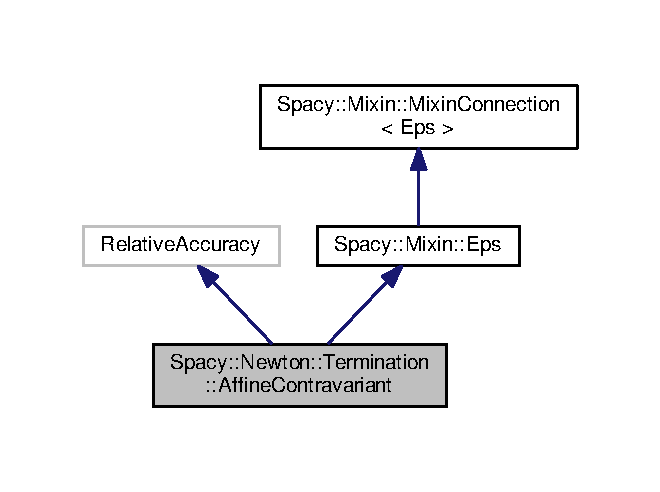
\includegraphics[width=310pt]{classSpacy_1_1Newton_1_1Termination_1_1AffineContravariant__inherit__graph}
\end{center}
\end{figure}


\-Collaboration diagram for \-Spacy\-:\-:\-Newton\-:\-:\-Termination\-:\-:\-Affine\-Contravariant\-:
\nopagebreak
\begin{figure}[H]
\begin{center}
\leavevmode
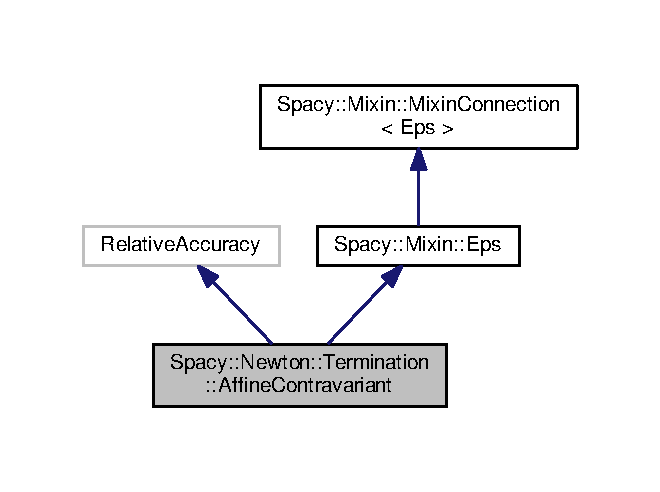
\includegraphics[width=310pt]{classSpacy_1_1Newton_1_1Termination_1_1AffineContravariant__coll__graph}
\end{center}
\end{figure}
\subsection*{\-Public \-Member \-Functions}
\begin{DoxyCompactItemize}
\item 
\hypertarget{classSpacy_1_1Newton_1_1Termination_1_1AffineContravariant_a84217ee3e52e0bc40ad2e1ecc13abf9a}{\hyperlink{classSpacy_1_1Newton_1_1Termination_1_1AffineContravariant_a84217ee3e52e0bc40ad2e1ecc13abf9a}{\-Affine\-Contravariant} (const \hyperlink{classSpacy_1_1C1Operator}{\-C1\-Operator} \&\-F, \hyperlink{classSpacy_1_1Real}{\-Real} relative\-Accuracy, \hyperlink{classSpacy_1_1Real}{\-Real} \hyperlink{classSpacy_1_1Mixin_1_1Eps_a812b99b0abc1d78a34b4114907f23f52}{eps})}\label{classSpacy_1_1Newton_1_1Termination_1_1AffineContravariant_a84217ee3e52e0bc40ad2e1ecc13abf9a}

\begin{DoxyCompactList}\small\item\em \-Constructor. \end{DoxyCompactList}\item 
bool \hyperlink{classSpacy_1_1Newton_1_1Termination_1_1AffineContravariant_a16b9829fd882e948b5d273b80c549f4b}{operator()} (\hyperlink{classSpacy_1_1DampingFactor}{\-Damping\-Factor} nu, const \hyperlink{classSpacy_1_1Vector}{\-Vector} \&x, const \hyperlink{classSpacy_1_1Vector}{\-Vector} \&) const 
\begin{DoxyCompactList}\small\item\em \-Apply termination criterion. \end{DoxyCompactList}\item 
\hypertarget{classSpacy_1_1Mixin_1_1Eps_a6b4c38a60848c0ab665fb3a81e181786}{void {\bfseries set\-Eps} (\hyperlink{classSpacy_1_1Real}{\-Real} \hyperlink{classSpacy_1_1Mixin_1_1Eps_a812b99b0abc1d78a34b4114907f23f52}{eps})}\label{classSpacy_1_1Mixin_1_1Eps_a6b4c38a60848c0ab665fb3a81e181786}

\item 
\hypertarget{classSpacy_1_1Mixin_1_1Eps_a812b99b0abc1d78a34b4114907f23f52}{\hyperlink{classSpacy_1_1Real}{\-Real} \hyperlink{classSpacy_1_1Mixin_1_1Eps_a812b99b0abc1d78a34b4114907f23f52}{eps} () const noexcept}\label{classSpacy_1_1Mixin_1_1Eps_a812b99b0abc1d78a34b4114907f23f52}

\begin{DoxyCompactList}\small\item\em \-Access $\varepsilon$. \end{DoxyCompactList}\item 
\hypertarget{classSpacy_1_1Mixin_1_1Eps_abd50a47b32614a950189855775a09d05}{\hyperlink{classSpacy_1_1Real}{\-Real} \hyperlink{classSpacy_1_1Mixin_1_1Eps_abd50a47b32614a950189855775a09d05}{sqrt\-Eps} () const noexcept}\label{classSpacy_1_1Mixin_1_1Eps_abd50a47b32614a950189855775a09d05}

\begin{DoxyCompactList}\small\item\em \-Access $\sqrt\varepsilon$. \end{DoxyCompactList}\item 
\hypertarget{classSpacy_1_1Mixin_1_1Eps_a4bbca3a4afc878d1a20b6335f35e58f7}{\hyperlink{classSpacy_1_1Real}{\-Real} \hyperlink{classSpacy_1_1Mixin_1_1Eps_a4bbca3a4afc878d1a20b6335f35e58f7}{cbrt\-Eps} () const noexcept}\label{classSpacy_1_1Mixin_1_1Eps_a4bbca3a4afc878d1a20b6335f35e58f7}

\begin{DoxyCompactList}\small\item\em \-Access $\varepsilon^{1/3}$. \end{DoxyCompactList}\item 
\hypertarget{classSpacy_1_1Mixin_1_1Eps_a151216968daef3da5f5cdc0b957ce01b}{void \hyperlink{classSpacy_1_1Mixin_1_1Eps_a151216968daef3da5f5cdc0b957ce01b}{update} (\hyperlink{classSpacy_1_1Mixin_1_1Eps_af616ae8e55a645cefd4d2d4504d6705a}{\-Eps} $\ast$changed\-Subject)}\label{classSpacy_1_1Mixin_1_1Eps_a151216968daef3da5f5cdc0b957ce01b}

\begin{DoxyCompactList}\small\item\em update function for observer pattern. \end{DoxyCompactList}\item 
\hypertarget{classSpacy_1_1Mixin_1_1MixinConnection_abb5520ee6b22dd993d78f142939a1ed4}{void \hyperlink{classSpacy_1_1Mixin_1_1MixinConnection_abb5520ee6b22dd993d78f142939a1ed4}{attach} (\hyperlink{classSpacy_1_1Mixin_1_1Eps_af616ae8e55a645cefd4d2d4504d6705a}{\-Eps} \&observer)}\label{classSpacy_1_1Mixin_1_1MixinConnection_abb5520ee6b22dd993d78f142939a1ed4}

\begin{DoxyCompactList}\small\item\em \-Attach observer. \end{DoxyCompactList}\item 
\hypertarget{classSpacy_1_1Mixin_1_1MixinConnection_adda739590c487679c26f60e50aedb73f}{void \hyperlink{classSpacy_1_1Mixin_1_1MixinConnection_adda739590c487679c26f60e50aedb73f}{detach} (\hyperlink{classSpacy_1_1Mixin_1_1Eps_af616ae8e55a645cefd4d2d4504d6705a}{\-Eps} \&observer)}\label{classSpacy_1_1Mixin_1_1MixinConnection_adda739590c487679c26f60e50aedb73f}

\begin{DoxyCompactList}\small\item\em \-Detach observer. \end{DoxyCompactList}\item 
\hypertarget{classSpacy_1_1Mixin_1_1MixinConnection_a1ddeaa78a3bb4a38c2cca36d1f99fe36}{void \hyperlink{classSpacy_1_1Mixin_1_1MixinConnection_a1ddeaa78a3bb4a38c2cca36d1f99fe36}{notify} ()}\label{classSpacy_1_1Mixin_1_1MixinConnection_a1ddeaa78a3bb4a38c2cca36d1f99fe36}

\begin{DoxyCompactList}\small\item\em \-Notify observers about changes. \end{DoxyCompactList}\end{DoxyCompactItemize}


\subsection{\-Detailed \-Description}
\-Affine contravariant relative error criterion. 

\subsection{\-Member \-Function \-Documentation}
\hypertarget{classSpacy_1_1Newton_1_1Termination_1_1AffineContravariant_a16b9829fd882e948b5d273b80c549f4b}{\index{\-Spacy\-::\-Newton\-::\-Termination\-::\-Affine\-Contravariant@{\-Spacy\-::\-Newton\-::\-Termination\-::\-Affine\-Contravariant}!operator()@{operator()}}
\index{operator()@{operator()}!Spacy::Newton::Termination::AffineContravariant@{\-Spacy\-::\-Newton\-::\-Termination\-::\-Affine\-Contravariant}}
\subsubsection[{operator()}]{\setlength{\rightskip}{0pt plus 5cm}bool \-Spacy\-::\-Newton\-::\-Termination\-::\-Affine\-Contravariant\-::operator() (
\begin{DoxyParamCaption}
\item[{{\bf \-Damping\-Factor}}]{nu, }
\item[{const {\bf \-Vector} \&}]{x, }
\item[{const {\bf \-Vector} \&}]{}
\end{DoxyParamCaption}
) const}}\label{classSpacy_1_1Newton_1_1Termination_1_1AffineContravariant_a16b9829fd882e948b5d273b80c549f4b}


\-Apply termination criterion. 


\begin{DoxyParams}{\-Parameters}
{\em nu} & damping factor \\
\hline
{\em x} & iterate \\
\hline
\end{DoxyParams}
\begin{DoxyReturn}{\-Returns}
true if $\nu=1$ and $ \|F(x)\|<rel_acc\|F(x_0)\| $, else false 
\end{DoxyReturn}


\-The documentation for this class was generated from the following file\-:\begin{DoxyCompactItemize}
\item 
/home/travis/build/spacy-\/dev/\-Spacy/\-Spacy/\-Algorithm/\-Newton/termination\-Criteria.\-hh\end{DoxyCompactItemize}

\hypertarget{classSpacy_1_1Newton_1_1Damping_1_1AffineCovariant}{\section{\-Spacy\-:\-:\-Newton\-:\-:\-Damping\-:\-:\-Affine\-Covariant \-Class \-Reference}
\label{classSpacy_1_1Newton_1_1Damping_1_1AffineCovariant}\index{\-Spacy\-::\-Newton\-::\-Damping\-::\-Affine\-Covariant@{\-Spacy\-::\-Newton\-::\-Damping\-::\-Affine\-Covariant}}
}


\-Affine covariant damping strategy as described in.  




{\ttfamily \#include $<$damping\-Strategies.\-hh$>$}



\-Inheritance diagram for \-Spacy\-:\-:\-Newton\-:\-:\-Damping\-:\-:\-Affine\-Covariant\-:
\nopagebreak
\begin{figure}[H]
\begin{center}
\leavevmode
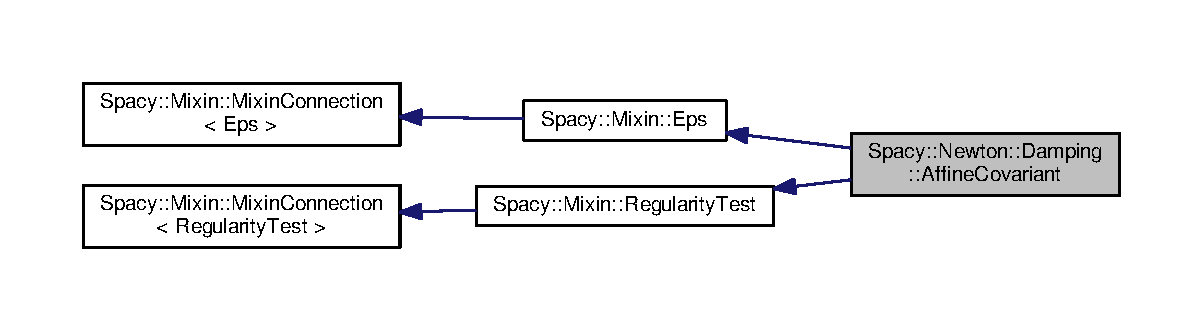
\includegraphics[width=350pt]{classSpacy_1_1Newton_1_1Damping_1_1AffineCovariant__inherit__graph}
\end{center}
\end{figure}


\-Collaboration diagram for \-Spacy\-:\-:\-Newton\-:\-:\-Damping\-:\-:\-Affine\-Covariant\-:
\nopagebreak
\begin{figure}[H]
\begin{center}
\leavevmode
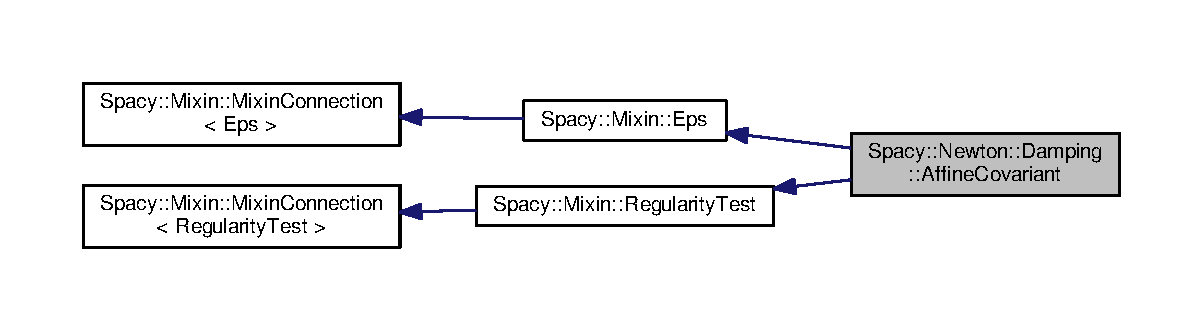
\includegraphics[width=350pt]{classSpacy_1_1Newton_1_1Damping_1_1AffineCovariant__coll__graph}
\end{center}
\end{figure}
\subsection*{\-Public \-Member \-Functions}
\begin{DoxyCompactItemize}
\item 
\hypertarget{classSpacy_1_1Newton_1_1Damping_1_1AffineCovariant_abf3615a91c70a145759d74eff761ec51}{\hyperlink{classSpacy_1_1Newton_1_1Damping_1_1AffineCovariant_abf3615a91c70a145759d74eff761ec51}{\-Affine\-Covariant} (const \hyperlink{classSpacy_1_1C1Operator}{\-C1\-Operator} \&\-F)}\label{classSpacy_1_1Newton_1_1Damping_1_1AffineCovariant_abf3615a91c70a145759d74eff761ec51}

\begin{DoxyCompactList}\small\item\em \-Constructor. \end{DoxyCompactList}\item 
\hypertarget{classSpacy_1_1Newton_1_1Damping_1_1AffineCovariant_a451040d8a986f1ae912b34713ced26ec}{\hyperlink{classSpacy_1_1DampingFactor}{\-Damping\-Factor} \hyperlink{classSpacy_1_1Newton_1_1Damping_1_1AffineCovariant_a451040d8a986f1ae912b34713ced26ec}{operator()} (const std\-::function$<$ \hyperlink{classSpacy_1_1Vector}{\-Vector}(const \hyperlink{classSpacy_1_1Vector}{\-Vector} \&)$>$ \&\-D\-F\-Inv\-\_\-, const \hyperlink{classSpacy_1_1Vector}{\-Vector} \&x, const \hyperlink{classSpacy_1_1Vector}{\-Vector} \&dx) const }\label{classSpacy_1_1Newton_1_1Damping_1_1AffineCovariant_a451040d8a986f1ae912b34713ced26ec}

\begin{DoxyCompactList}\small\item\em \-Compute damping factor. \end{DoxyCompactList}\item 
\hypertarget{classSpacy_1_1Mixin_1_1Eps_a818ab6dfab5e4eea583e1302bcc621f8}{void {\bfseries set\-\_\-eps} (\hyperlink{classSpacy_1_1Real}{\-Real} \hyperlink{classSpacy_1_1Mixin_1_1Eps_a812b99b0abc1d78a34b4114907f23f52}{eps})}\label{classSpacy_1_1Mixin_1_1Eps_a818ab6dfab5e4eea583e1302bcc621f8}

\item 
\hypertarget{classSpacy_1_1Mixin_1_1Eps_a812b99b0abc1d78a34b4114907f23f52}{\hyperlink{classSpacy_1_1Real}{\-Real} \hyperlink{classSpacy_1_1Mixin_1_1Eps_a812b99b0abc1d78a34b4114907f23f52}{eps} () const noexcept}\label{classSpacy_1_1Mixin_1_1Eps_a812b99b0abc1d78a34b4114907f23f52}

\begin{DoxyCompactList}\small\item\em \-Access $\varepsilon$. \end{DoxyCompactList}\item 
\hypertarget{classSpacy_1_1Mixin_1_1Eps_a1c1b0ed7f14ed4967dc7da9295a136d4}{\hyperlink{classSpacy_1_1Real}{\-Real} \hyperlink{classSpacy_1_1Mixin_1_1Eps_a1c1b0ed7f14ed4967dc7da9295a136d4}{sqrt\-\_\-eps} () const noexcept}\label{classSpacy_1_1Mixin_1_1Eps_a1c1b0ed7f14ed4967dc7da9295a136d4}

\begin{DoxyCompactList}\small\item\em \-Access $\sqrt\varepsilon$. \end{DoxyCompactList}\item 
\hypertarget{classSpacy_1_1Mixin_1_1Eps_a91dbe45e297be2bc53f1a96107a58c64}{\hyperlink{classSpacy_1_1Real}{\-Real} \hyperlink{classSpacy_1_1Mixin_1_1Eps_a91dbe45e297be2bc53f1a96107a58c64}{cbrt\-\_\-eps} () const noexcept}\label{classSpacy_1_1Mixin_1_1Eps_a91dbe45e297be2bc53f1a96107a58c64}

\begin{DoxyCompactList}\small\item\em \-Access $\varepsilon^{1/3}$. \end{DoxyCompactList}\item 
\hypertarget{classSpacy_1_1Mixin_1_1Eps_a151216968daef3da5f5cdc0b957ce01b}{void \hyperlink{classSpacy_1_1Mixin_1_1Eps_a151216968daef3da5f5cdc0b957ce01b}{update} (\hyperlink{classSpacy_1_1Mixin_1_1Eps_af616ae8e55a645cefd4d2d4504d6705a}{\-Eps} $\ast$changed\-Subject)}\label{classSpacy_1_1Mixin_1_1Eps_a151216968daef3da5f5cdc0b957ce01b}

\begin{DoxyCompactList}\small\item\em update function for observer pattern. \end{DoxyCompactList}\item 
\hypertarget{classSpacy_1_1Mixin_1_1MixinConnection_abb5520ee6b22dd993d78f142939a1ed4}{void \hyperlink{classSpacy_1_1Mixin_1_1MixinConnection_abb5520ee6b22dd993d78f142939a1ed4}{attach} (\hyperlink{classSpacy_1_1Mixin_1_1Eps_af616ae8e55a645cefd4d2d4504d6705a}{\-Eps} \&observer)}\label{classSpacy_1_1Mixin_1_1MixinConnection_abb5520ee6b22dd993d78f142939a1ed4}

\begin{DoxyCompactList}\small\item\em \-Attach observer. \end{DoxyCompactList}\item 
\hypertarget{classSpacy_1_1Mixin_1_1MixinConnection_adda739590c487679c26f60e50aedb73f}{void \hyperlink{classSpacy_1_1Mixin_1_1MixinConnection_adda739590c487679c26f60e50aedb73f}{detach} (\hyperlink{classSpacy_1_1Mixin_1_1Eps_af616ae8e55a645cefd4d2d4504d6705a}{\-Eps} \&observer)}\label{classSpacy_1_1Mixin_1_1MixinConnection_adda739590c487679c26f60e50aedb73f}

\begin{DoxyCompactList}\small\item\em \-Detach observer. \end{DoxyCompactList}\item 
\hypertarget{classSpacy_1_1Mixin_1_1MixinConnection_a1ddeaa78a3bb4a38c2cca36d1f99fe36}{void \hyperlink{classSpacy_1_1Mixin_1_1MixinConnection_a1ddeaa78a3bb4a38c2cca36d1f99fe36}{notify} ()}\label{classSpacy_1_1Mixin_1_1MixinConnection_a1ddeaa78a3bb4a38c2cca36d1f99fe36}

\begin{DoxyCompactList}\small\item\em \-Notify observers about changes. \end{DoxyCompactList}\item 
\hypertarget{classSpacy_1_1Mixin_1_1RegularityTest_a682ce022b0b5493e48f50f693ed64082}{void \hyperlink{classSpacy_1_1Mixin_1_1RegularityTest_a682ce022b0b5493e48f50f693ed64082}{set\-Lower\-Bound} (\hyperlink{classSpacy_1_1DampingFactor}{\-Damping\-Factor} lower\-Bound)}\label{classSpacy_1_1Mixin_1_1RegularityTest_a682ce022b0b5493e48f50f693ed64082}

\begin{DoxyCompactList}\small\item\em \-Set lower bound of regularity test for termination criteria. \end{DoxyCompactList}\item 
\hypertarget{classSpacy_1_1Mixin_1_1RegularityTest_a576995201badbfaee2064bf0d7749257}{\hyperlink{classSpacy_1_1DampingFactor}{\-Damping\-Factor} {\bfseries get\-Lower\-Bound} () const noexcept}\label{classSpacy_1_1Mixin_1_1RegularityTest_a576995201badbfaee2064bf0d7749257}

\item 
bool \hyperlink{classSpacy_1_1Mixin_1_1RegularityTest_acb6b3e8c76ebdbded0ec610959513caf}{regularity\-Test\-Passed} (\hyperlink{classSpacy_1_1DampingFactor}{\-Damping\-Factor} nu) const noexcept
\begin{DoxyCompactList}\small\item\em \-Apply regularity test. \end{DoxyCompactList}\item 
bool \hyperlink{classSpacy_1_1Mixin_1_1RegularityTest_aeb1a3b051bafc9da9be1df354c652812}{regularity\-Test\-Failed} (\hyperlink{classSpacy_1_1DampingFactor}{\-Damping\-Factor} nu) const noexcept
\begin{DoxyCompactList}\small\item\em \-Apply regularity test. \end{DoxyCompactList}\item 
\hypertarget{classSpacy_1_1Mixin_1_1RegularityTest_a1a6191e20f84025cec8b10ec63ab94ac}{void \hyperlink{classSpacy_1_1Mixin_1_1RegularityTest_a1a6191e20f84025cec8b10ec63ab94ac}{update} (\hyperlink{classSpacy_1_1Mixin_1_1RegularityTest_a548d9d45c31c7833266bd3b20dc1aa7e}{\-Regularity\-Test} $\ast$changed\-Subject)}\label{classSpacy_1_1Mixin_1_1RegularityTest_a1a6191e20f84025cec8b10ec63ab94ac}

\begin{DoxyCompactList}\small\item\em update function for observer pattern. \end{DoxyCompactList}\item 
\hypertarget{classSpacy_1_1Mixin_1_1MixinConnection_abb5520ee6b22dd993d78f142939a1ed4}{void \hyperlink{classSpacy_1_1Mixin_1_1MixinConnection_abb5520ee6b22dd993d78f142939a1ed4}{attach} (\hyperlink{classSpacy_1_1Mixin_1_1RegularityTest_a548d9d45c31c7833266bd3b20dc1aa7e}{\-Regularity\-Test} \&observer)}\label{classSpacy_1_1Mixin_1_1MixinConnection_abb5520ee6b22dd993d78f142939a1ed4}

\begin{DoxyCompactList}\small\item\em \-Attach observer. \end{DoxyCompactList}\item 
\hypertarget{classSpacy_1_1Mixin_1_1MixinConnection_adda739590c487679c26f60e50aedb73f}{void \hyperlink{classSpacy_1_1Mixin_1_1MixinConnection_adda739590c487679c26f60e50aedb73f}{detach} (\hyperlink{classSpacy_1_1Mixin_1_1RegularityTest_a548d9d45c31c7833266bd3b20dc1aa7e}{\-Regularity\-Test} \&observer)}\label{classSpacy_1_1Mixin_1_1MixinConnection_adda739590c487679c26f60e50aedb73f}

\begin{DoxyCompactList}\small\item\em \-Detach observer. \end{DoxyCompactList}\item 
\hypertarget{classSpacy_1_1Mixin_1_1MixinConnection_a1ddeaa78a3bb4a38c2cca36d1f99fe36}{void \hyperlink{classSpacy_1_1Mixin_1_1MixinConnection_a1ddeaa78a3bb4a38c2cca36d1f99fe36}{notify} ()}\label{classSpacy_1_1Mixin_1_1MixinConnection_a1ddeaa78a3bb4a38c2cca36d1f99fe36}

\begin{DoxyCompactList}\small\item\em \-Notify observers about changes. \end{DoxyCompactList}\end{DoxyCompactItemize}


\subsection{\-Detailed \-Description}
\-Affine covariant damping strategy as described in. 

\cite{Deuflhard2004} \mbox{[}\-Sec. 3.\-3\mbox{]}. 

\subsection{\-Member \-Function \-Documentation}
\hypertarget{classSpacy_1_1Mixin_1_1RegularityTest_acb6b3e8c76ebdbded0ec610959513caf}{\index{\-Spacy\-::\-Newton\-::\-Damping\-::\-Affine\-Covariant@{\-Spacy\-::\-Newton\-::\-Damping\-::\-Affine\-Covariant}!regularity\-Test\-Passed@{regularity\-Test\-Passed}}
\index{regularity\-Test\-Passed@{regularity\-Test\-Passed}!Spacy::Newton::Damping::AffineCovariant@{\-Spacy\-::\-Newton\-::\-Damping\-::\-Affine\-Covariant}}
\subsubsection[{regularity\-Test\-Passed}]{\setlength{\rightskip}{0pt plus 5cm}bool {\bf \-Spacy\-::\-Mixin\-::\-Regularity\-Test\-::regularity\-Test\-Passed} (
\begin{DoxyParamCaption}
\item[{{\bf \-Damping\-Factor}}]{nu}
\end{DoxyParamCaption}
) const\hspace{0.3cm}{\ttfamily  \mbox{[}inherited\mbox{]}}}}\label{classSpacy_1_1Mixin_1_1RegularityTest_acb6b3e8c76ebdbded0ec610959513caf}


\-Apply regularity test. 


\begin{DoxyParams}{\-Parameters}
{\em nu} & damping factor \\
\hline
\end{DoxyParams}
\begin{DoxyReturn}{\-Returns}
$nu > lowerBound_$ 
\end{DoxyReturn}
\hypertarget{classSpacy_1_1Mixin_1_1RegularityTest_aeb1a3b051bafc9da9be1df354c652812}{\index{\-Spacy\-::\-Newton\-::\-Damping\-::\-Affine\-Covariant@{\-Spacy\-::\-Newton\-::\-Damping\-::\-Affine\-Covariant}!regularity\-Test\-Failed@{regularity\-Test\-Failed}}
\index{regularity\-Test\-Failed@{regularity\-Test\-Failed}!Spacy::Newton::Damping::AffineCovariant@{\-Spacy\-::\-Newton\-::\-Damping\-::\-Affine\-Covariant}}
\subsubsection[{regularity\-Test\-Failed}]{\setlength{\rightskip}{0pt plus 5cm}bool {\bf \-Spacy\-::\-Mixin\-::\-Regularity\-Test\-::regularity\-Test\-Failed} (
\begin{DoxyParamCaption}
\item[{{\bf \-Damping\-Factor}}]{nu}
\end{DoxyParamCaption}
) const\hspace{0.3cm}{\ttfamily  \mbox{[}inherited\mbox{]}}}}\label{classSpacy_1_1Mixin_1_1RegularityTest_aeb1a3b051bafc9da9be1df354c652812}


\-Apply regularity test. 


\begin{DoxyParams}{\-Parameters}
{\em nu} & damping factor \\
\hline
\end{DoxyParams}
\begin{DoxyReturn}{\-Returns}
$nu <= lowerBound_$ 
\end{DoxyReturn}


\-The documentation for this class was generated from the following file\-:\begin{DoxyCompactItemize}
\item 
/home/travis/build/spacy-\/dev/\-Spacy/\-Spacy/\-Algorithm/\-Newton/damping\-Strategies.\-hh\end{DoxyCompactItemize}

\hypertarget{classSpacy_1_1Newton_1_1Termination_1_1AffineCovariant}{\section{Spacy\-:\-:Newton\-:\-:Termination\-:\-:Affine\-Covariant Class Reference}
\label{classSpacy_1_1Newton_1_1Termination_1_1AffineCovariant}\index{Spacy\-::\-Newton\-::\-Termination\-::\-Affine\-Covariant@{Spacy\-::\-Newton\-::\-Termination\-::\-Affine\-Covariant}}
}


Affine covariant relative error criterion.  




{\ttfamily \#include $<$termination\-Criteria.\-hh$>$}



Inheritance diagram for Spacy\-:\-:Newton\-:\-:Termination\-:\-:Affine\-Covariant\-:
\nopagebreak
\begin{figure}[H]
\begin{center}
\leavevmode
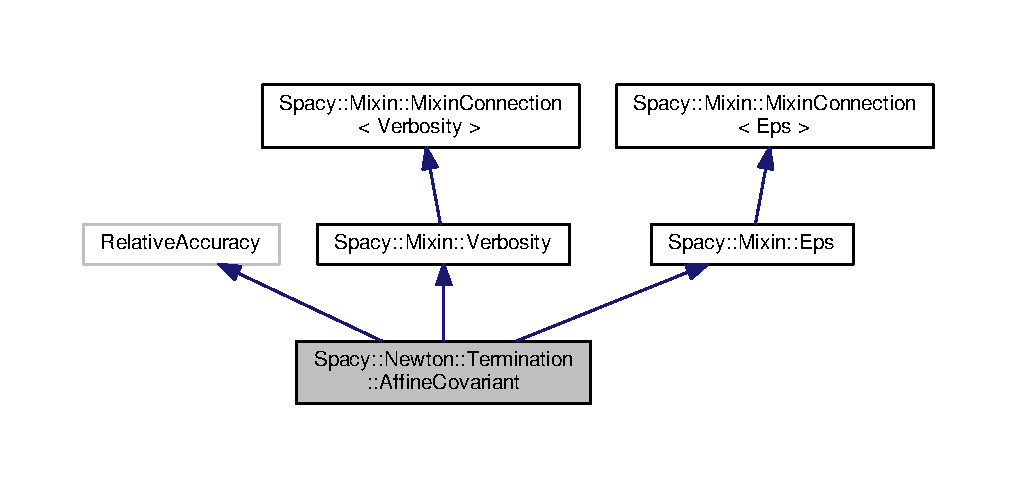
\includegraphics[width=317pt]{classSpacy_1_1Newton_1_1Termination_1_1AffineCovariant__inherit__graph}
\end{center}
\end{figure}


Collaboration diagram for Spacy\-:\-:Newton\-:\-:Termination\-:\-:Affine\-Covariant\-:
\nopagebreak
\begin{figure}[H]
\begin{center}
\leavevmode
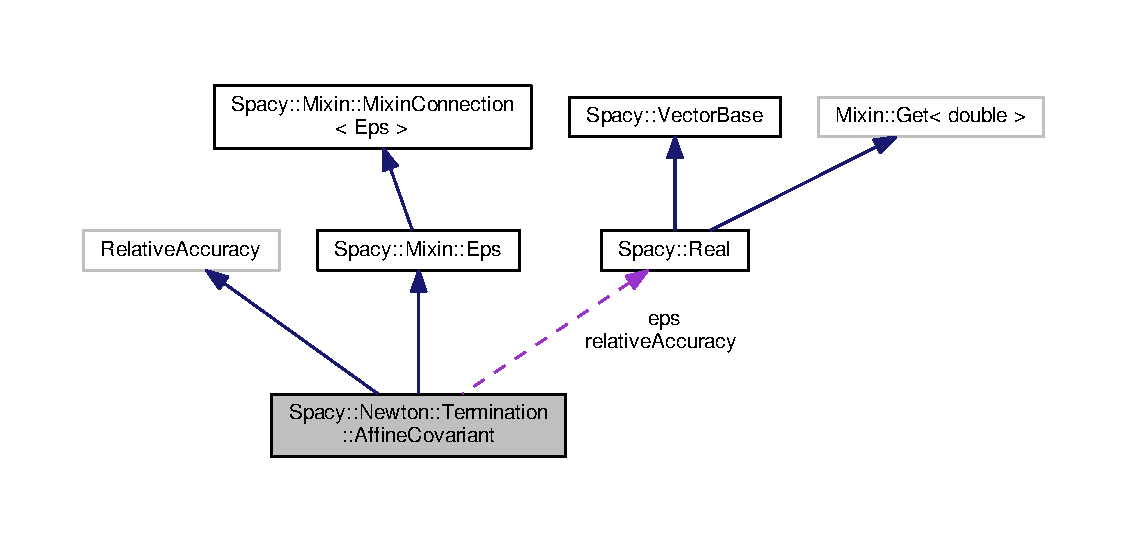
\includegraphics[width=350pt]{classSpacy_1_1Newton_1_1Termination_1_1AffineCovariant__coll__graph}
\end{center}
\end{figure}
\subsection*{Public Member Functions}
\begin{DoxyCompactItemize}
\item 
\hypertarget{classSpacy_1_1Newton_1_1Termination_1_1AffineCovariant_aa725dc117c4c563d4c1b0ca0f14feea9}{\hyperlink{classSpacy_1_1Newton_1_1Termination_1_1AffineCovariant_aa725dc117c4c563d4c1b0ca0f14feea9}{D\-E\-F\-I\-N\-E\-\_\-\-L\-O\-G\-\_\-\-T\-A\-G} (static constexpr const char $\ast$covariant\-\_\-log\-\_\-tag=\char`\"{}Covariant\-Termination\-Strategy\char`\"{}) Affine\-Covariant(const \hyperlink{classSpacy_1_1C1Operator}{C1\-Operator} \&}\label{classSpacy_1_1Newton_1_1Termination_1_1AffineCovariant_aa725dc117c4c563d4c1b0ca0f14feea9}

\begin{DoxyCompactList}\small\item\em Constuctor. \end{DoxyCompactList}\item 
bool \hyperlink{classSpacy_1_1Newton_1_1Termination_1_1AffineCovariant_aa33460372120d1ddcd3daf7c79140dcf}{operator()} (\hyperlink{classSpacy_1_1DampingFactor}{Damping\-Factor} nu, const \hyperlink{classSpacy_1_1Vector}{Vector} \&x, const \hyperlink{classSpacy_1_1Vector}{Vector} \&dx) const 
\begin{DoxyCompactList}\small\item\em Apply termination criterion. \end{DoxyCompactList}\item 
\hypertarget{classSpacy_1_1Mixin_1_1Eps_a818ab6dfab5e4eea583e1302bcc621f8}{void {\bfseries set\-\_\-eps} (\hyperlink{classSpacy_1_1Real}{Real} eps)}\label{classSpacy_1_1Mixin_1_1Eps_a818ab6dfab5e4eea583e1302bcc621f8}

\item 
\hypertarget{classSpacy_1_1Mixin_1_1Eps_a812b99b0abc1d78a34b4114907f23f52}{\hyperlink{classSpacy_1_1Real}{Real} \hyperlink{classSpacy_1_1Mixin_1_1Eps_a812b99b0abc1d78a34b4114907f23f52}{eps} () const noexcept}\label{classSpacy_1_1Mixin_1_1Eps_a812b99b0abc1d78a34b4114907f23f52}

\begin{DoxyCompactList}\small\item\em Access $\varepsilon$. \end{DoxyCompactList}\item 
\hypertarget{classSpacy_1_1Mixin_1_1Eps_a1c1b0ed7f14ed4967dc7da9295a136d4}{\hyperlink{classSpacy_1_1Real}{Real} \hyperlink{classSpacy_1_1Mixin_1_1Eps_a1c1b0ed7f14ed4967dc7da9295a136d4}{sqrt\-\_\-eps} () const noexcept}\label{classSpacy_1_1Mixin_1_1Eps_a1c1b0ed7f14ed4967dc7da9295a136d4}

\begin{DoxyCompactList}\small\item\em Access $\sqrt\varepsilon$. \end{DoxyCompactList}\item 
\hypertarget{classSpacy_1_1Mixin_1_1Eps_a91dbe45e297be2bc53f1a96107a58c64}{\hyperlink{classSpacy_1_1Real}{Real} \hyperlink{classSpacy_1_1Mixin_1_1Eps_a91dbe45e297be2bc53f1a96107a58c64}{cbrt\-\_\-eps} () const noexcept}\label{classSpacy_1_1Mixin_1_1Eps_a91dbe45e297be2bc53f1a96107a58c64}

\begin{DoxyCompactList}\small\item\em Access $\varepsilon^{1/3}$. \end{DoxyCompactList}\item 
\hypertarget{classSpacy_1_1Mixin_1_1Eps_a151216968daef3da5f5cdc0b957ce01b}{void \hyperlink{classSpacy_1_1Mixin_1_1Eps_a151216968daef3da5f5cdc0b957ce01b}{update} (\hyperlink{classSpacy_1_1Mixin_1_1Eps_af616ae8e55a645cefd4d2d4504d6705a}{Eps} $\ast$changed\-Subject)}\label{classSpacy_1_1Mixin_1_1Eps_a151216968daef3da5f5cdc0b957ce01b}

\begin{DoxyCompactList}\small\item\em update function for observer pattern. \end{DoxyCompactList}\item 
\hypertarget{classSpacy_1_1Mixin_1_1MixinConnection_abb5520ee6b22dd993d78f142939a1ed4}{void \hyperlink{classSpacy_1_1Mixin_1_1MixinConnection_abb5520ee6b22dd993d78f142939a1ed4}{attach} (\hyperlink{classSpacy_1_1Mixin_1_1Eps_af616ae8e55a645cefd4d2d4504d6705a}{Eps} \&observer)}\label{classSpacy_1_1Mixin_1_1MixinConnection_abb5520ee6b22dd993d78f142939a1ed4}

\begin{DoxyCompactList}\small\item\em Attach observer. \end{DoxyCompactList}\item 
\hypertarget{classSpacy_1_1Mixin_1_1MixinConnection_adda739590c487679c26f60e50aedb73f}{void \hyperlink{classSpacy_1_1Mixin_1_1MixinConnection_adda739590c487679c26f60e50aedb73f}{detach} (\hyperlink{classSpacy_1_1Mixin_1_1Eps_af616ae8e55a645cefd4d2d4504d6705a}{Eps} \&observer)}\label{classSpacy_1_1Mixin_1_1MixinConnection_adda739590c487679c26f60e50aedb73f}

\begin{DoxyCompactList}\small\item\em Detach observer. \end{DoxyCompactList}\item 
\hypertarget{classSpacy_1_1Mixin_1_1MixinConnection_a1ddeaa78a3bb4a38c2cca36d1f99fe36}{void \hyperlink{classSpacy_1_1Mixin_1_1MixinConnection_a1ddeaa78a3bb4a38c2cca36d1f99fe36}{notify} ()}\label{classSpacy_1_1Mixin_1_1MixinConnection_a1ddeaa78a3bb4a38c2cca36d1f99fe36}

\begin{DoxyCompactList}\small\item\em Notify observers about changes. \end{DoxyCompactList}\end{DoxyCompactItemize}
\subsection*{Public Attributes}
\begin{DoxyCompactItemize}
\item 
\hypertarget{classSpacy_1_1Newton_1_1Termination_1_1AffineCovariant_a3b098c6070c5928dc9b88a9fce2a3654}{\hyperlink{classSpacy_1_1Real}{Real} {\bfseries relative\-Accuracy}}\label{classSpacy_1_1Newton_1_1Termination_1_1AffineCovariant_a3b098c6070c5928dc9b88a9fce2a3654}

\item 
\hypertarget{classSpacy_1_1Newton_1_1Termination_1_1AffineCovariant_a666203e1caa70afbc51bdca583201f0d}{\hyperlink{classSpacy_1_1Real}{Real} \hyperlink{classSpacy_1_1Real}{Real} {\bfseries eps}}\label{classSpacy_1_1Newton_1_1Termination_1_1AffineCovariant_a666203e1caa70afbc51bdca583201f0d}

\end{DoxyCompactItemize}


\subsection{Detailed Description}
Affine covariant relative error criterion. 

\subsection{Member Function Documentation}
\hypertarget{classSpacy_1_1Newton_1_1Termination_1_1AffineCovariant_aa33460372120d1ddcd3daf7c79140dcf}{\index{Spacy\-::\-Newton\-::\-Termination\-::\-Affine\-Covariant@{Spacy\-::\-Newton\-::\-Termination\-::\-Affine\-Covariant}!operator()@{operator()}}
\index{operator()@{operator()}!Spacy::Newton::Termination::AffineCovariant@{Spacy\-::\-Newton\-::\-Termination\-::\-Affine\-Covariant}}
\subsubsection[{operator()}]{\setlength{\rightskip}{0pt plus 5cm}bool Spacy\-::\-Newton\-::\-Termination\-::\-Affine\-Covariant\-::operator() (
\begin{DoxyParamCaption}
\item[{{\bf Damping\-Factor}}]{nu, }
\item[{const {\bf Vector} \&}]{x, }
\item[{const {\bf Vector} \&}]{dx}
\end{DoxyParamCaption}
) const}}\label{classSpacy_1_1Newton_1_1Termination_1_1AffineCovariant_aa33460372120d1ddcd3daf7c79140dcf}


Apply termination criterion. 


\begin{DoxyParams}{Parameters}
{\em nu} & damping factor \\
\hline
{\em x} & iterate \\
\hline
{\em dx} & correction \\
\hline
\end{DoxyParams}
\begin{DoxyReturn}{Returns}
true if $\nu=1$ and $ \|dx\|<rel_acc\|x\| $ or $\|x\|=\|dx\|=0$, else false 
\end{DoxyReturn}


The documentation for this class was generated from the following file\-:\begin{DoxyCompactItemize}
\item 
/home/travis/build/spacy-\/dev/\-Spacy/\-Spacy/\-Algorithm/\-Newton/termination\-Criteria.\-hh\end{DoxyCompactItemize}

\hypertarget{classSpacy_1_1CompositeStep_1_1AffineCovariantSolver}{\section{\-Spacy\-:\-:\-Composite\-Step\-:\-:\-Affine\-Covariant\-Solver \-Class \-Reference}
\label{classSpacy_1_1CompositeStep_1_1AffineCovariantSolver}\index{\-Spacy\-::\-Composite\-Step\-::\-Affine\-Covariant\-Solver@{\-Spacy\-::\-Composite\-Step\-::\-Affine\-Covariant\-Solver}}
}


\-The affine covariant step method described in.  




{\ttfamily \#include $<$affine\-Covariant\-Solver.\-hh$>$}



\-Inheritance diagram for \-Spacy\-:\-:\-Composite\-Step\-:\-:\-Affine\-Covariant\-Solver\-:
\nopagebreak
\begin{figure}[H]
\begin{center}
\leavevmode
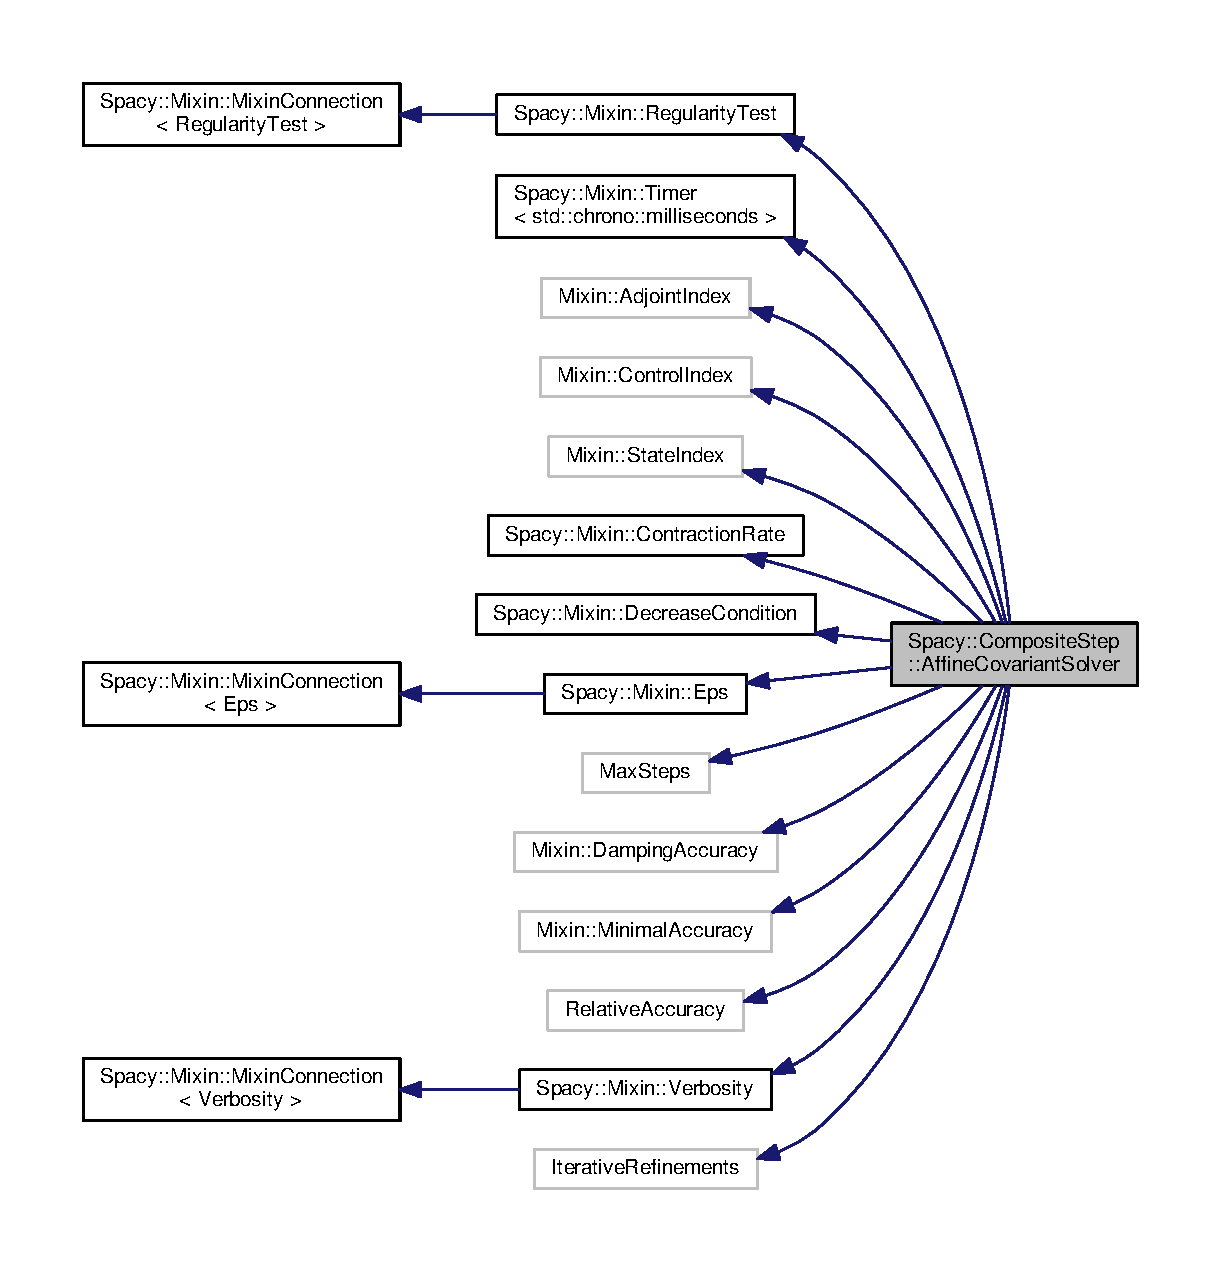
\includegraphics[width=350pt]{classSpacy_1_1CompositeStep_1_1AffineCovariantSolver__inherit__graph}
\end{center}
\end{figure}


\-Collaboration diagram for \-Spacy\-:\-:\-Composite\-Step\-:\-:\-Affine\-Covariant\-Solver\-:
\nopagebreak
\begin{figure}[H]
\begin{center}
\leavevmode
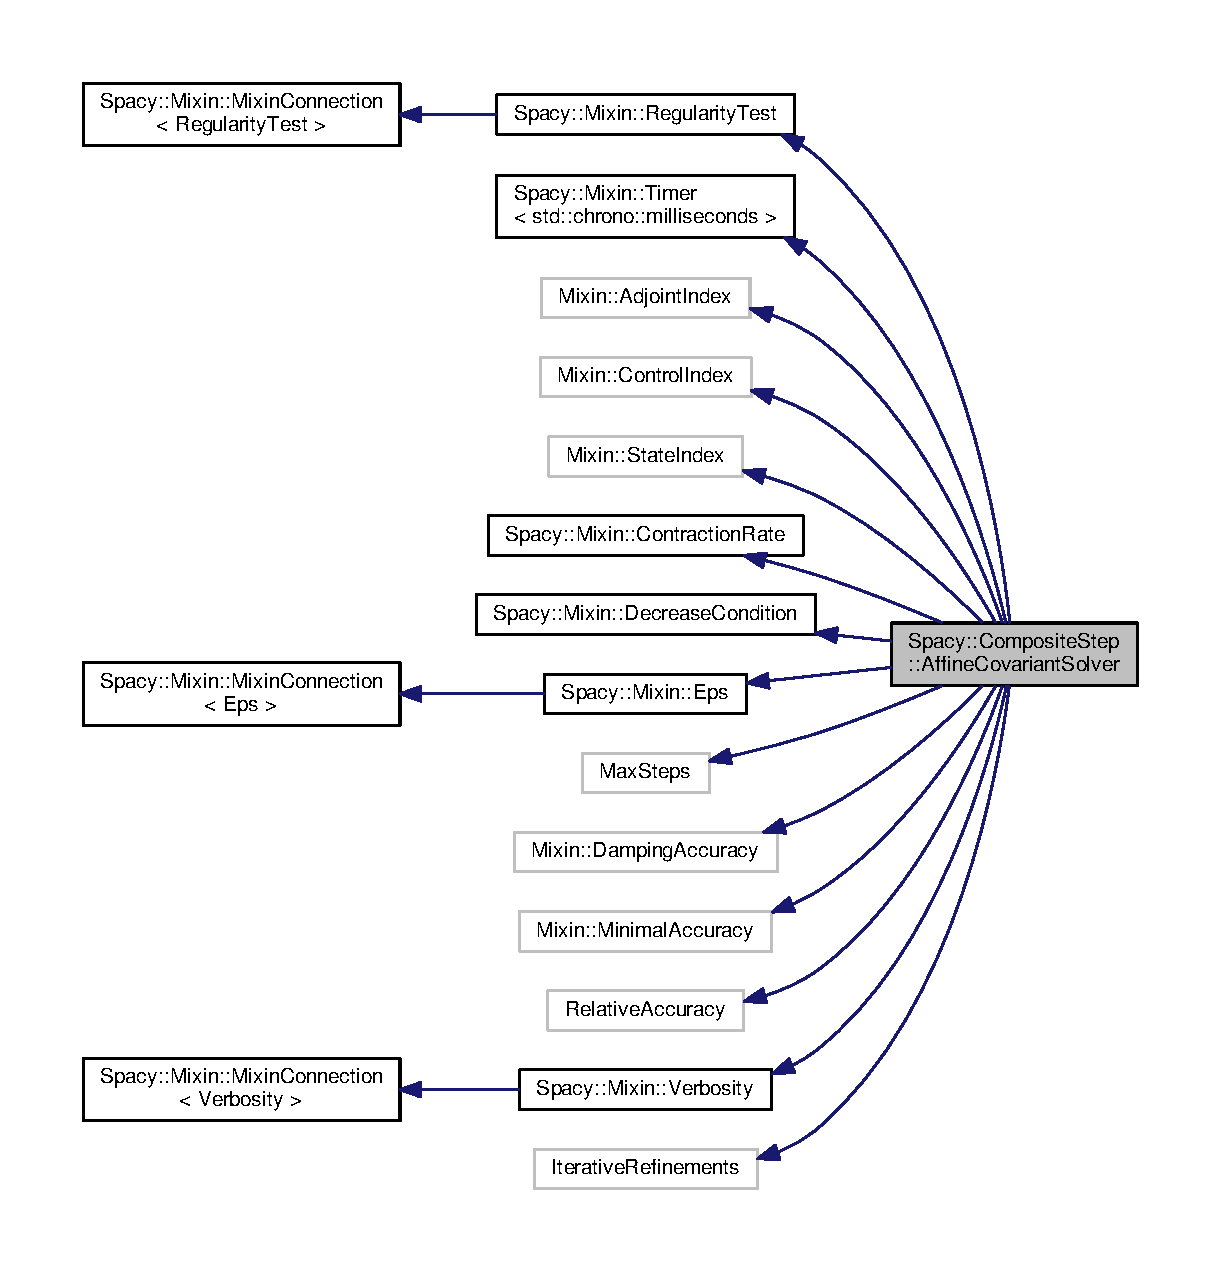
\includegraphics[width=350pt]{classSpacy_1_1CompositeStep_1_1AffineCovariantSolver__coll__graph}
\end{center}
\end{figure}
\subsection*{\-Public \-Member \-Functions}
\begin{DoxyCompactItemize}
\item 
\hyperlink{classSpacy_1_1CompositeStep_1_1AffineCovariantSolver_af81f7894dc2b7ee3533ab67d82195751}{\-Affine\-Covariant\-Solver} (\hyperlink{classSpacy_1_1C2Functional}{\-C2\-Functional} \-N, \hyperlink{classSpacy_1_1C2Functional}{\-C2\-Functional} \-L, \hyperlink{classSpacy_1_1VectorSpace}{\-Vector\-Space} \&domain)
\begin{DoxyCompactList}\small\item\em \-Constructor. \end{DoxyCompactList}\item 
\hypertarget{classSpacy_1_1CompositeStep_1_1AffineCovariantSolver_a1c29ce1bfa93809d9189021e248b957b}{{\bfseries \-Affine\-Covariant\-Solver} (\hyperlink{classSpacy_1_1C2Functional}{\-C2\-Functional} \-N, \hyperlink{classSpacy_1_1C2Functional}{\-C2\-Functional} \-L, \hyperlink{classSpacy_1_1VectorSpace}{\-Vector\-Space} \&domain, std\-::function$<$ \hyperlink{classSpacy_1_1Vector}{\-Vector}(const \hyperlink{classSpacy_1_1Vector}{\-Vector} \&, const \hyperlink{classSpacy_1_1Vector}{\-Vector} \&) $>$ retraction)}\label{classSpacy_1_1CompositeStep_1_1AffineCovariantSolver_a1c29ce1bfa93809d9189021e248b957b}

\item 
\hypertarget{classSpacy_1_1CompositeStep_1_1AffineCovariantSolver_ae79d78e682c85638ddf967e3f14ec151}{{\bfseries \-Affine\-Covariant\-Solver} (\hyperlink{classSpacy_1_1C2Functional}{\-C2\-Functional} \-N, \hyperlink{classSpacy_1_1C2Functional}{\-C2\-Functional} \-L, \hyperlink{classSpacy_1_1VectorSpace}{\-Vector\-Space} \&total\-Space, \hyperlink{classSpacy_1_1VectorSpace}{\-Vector\-Space} \&chart\-Space, std\-::function$<$ \hyperlink{classSpacy_1_1Vector}{\-Vector}(const \hyperlink{classSpacy_1_1Vector}{\-Vector} \&, const \hyperlink{classSpacy_1_1Vector}{\-Vector} \&) $>$ retraction, std\-::function$<$ \hyperlink{classSpacy_1_1Vector}{\-Vector}(const \hyperlink{classSpacy_1_1Vector}{\-Vector} \&, const \hyperlink{classSpacy_1_1Vector}{\-Vector} \&) $>$ dual\-Update)}\label{classSpacy_1_1CompositeStep_1_1AffineCovariantSolver_ae79d78e682c85638ddf967e3f14ec151}

\item 
\hypertarget{classSpacy_1_1CompositeStep_1_1AffineCovariantSolver_a010068164773b4062ec122b253a8226c}{\hyperlink{classSpacy_1_1Vector}{\-Vector} \hyperlink{classSpacy_1_1CompositeStep_1_1AffineCovariantSolver_a010068164773b4062ec122b253a8226c}{operator()} ()}\label{classSpacy_1_1CompositeStep_1_1AffineCovariantSolver_a010068164773b4062ec122b253a8226c}

\begin{DoxyCompactList}\small\item\em \-Compute solution. \end{DoxyCompactList}\item 
\hyperlink{classSpacy_1_1Vector}{\-Vector} \hyperlink{classSpacy_1_1CompositeStep_1_1AffineCovariantSolver_ae08612c2a1ca88d9a3746766bd5c1035}{operator()} (const \hyperlink{classSpacy_1_1Vector}{\-Vector} \&x0)
\begin{DoxyCompactList}\small\item\em \-Compute solution. \end{DoxyCompactList}\item 
\hypertarget{classSpacy_1_1Mixin_1_1RegularityTest_a682ce022b0b5493e48f50f693ed64082}{void \hyperlink{classSpacy_1_1Mixin_1_1RegularityTest_a682ce022b0b5493e48f50f693ed64082}{set\-Lower\-Bound} (\hyperlink{classSpacy_1_1DampingFactor}{\-Damping\-Factor} lower\-Bound)}\label{classSpacy_1_1Mixin_1_1RegularityTest_a682ce022b0b5493e48f50f693ed64082}

\begin{DoxyCompactList}\small\item\em \-Set lower bound of regularity test for termination criteria. \end{DoxyCompactList}\item 
\hypertarget{classSpacy_1_1Mixin_1_1RegularityTest_a576995201badbfaee2064bf0d7749257}{\hyperlink{classSpacy_1_1DampingFactor}{\-Damping\-Factor} {\bfseries get\-Lower\-Bound} () const noexcept}\label{classSpacy_1_1Mixin_1_1RegularityTest_a576995201badbfaee2064bf0d7749257}

\item 
bool \hyperlink{classSpacy_1_1Mixin_1_1RegularityTest_acb6b3e8c76ebdbded0ec610959513caf}{regularity\-Test\-Passed} (\hyperlink{classSpacy_1_1DampingFactor}{\-Damping\-Factor} nu) const noexcept
\begin{DoxyCompactList}\small\item\em \-Apply regularity test. \end{DoxyCompactList}\item 
bool \hyperlink{classSpacy_1_1Mixin_1_1RegularityTest_aeb1a3b051bafc9da9be1df354c652812}{regularity\-Test\-Failed} (\hyperlink{classSpacy_1_1DampingFactor}{\-Damping\-Factor} nu) const noexcept
\begin{DoxyCompactList}\small\item\em \-Apply regularity test. \end{DoxyCompactList}\item 
\hypertarget{classSpacy_1_1Mixin_1_1RegularityTest_a1a6191e20f84025cec8b10ec63ab94ac}{void \hyperlink{classSpacy_1_1Mixin_1_1RegularityTest_a1a6191e20f84025cec8b10ec63ab94ac}{update} (\hyperlink{classSpacy_1_1Mixin_1_1RegularityTest_a548d9d45c31c7833266bd3b20dc1aa7e}{\-Regularity\-Test} $\ast$changed\-Subject)}\label{classSpacy_1_1Mixin_1_1RegularityTest_a1a6191e20f84025cec8b10ec63ab94ac}

\begin{DoxyCompactList}\small\item\em update function for observer pattern. \end{DoxyCompactList}\item 
\hypertarget{classSpacy_1_1Mixin_1_1MixinConnection_abb5520ee6b22dd993d78f142939a1ed4}{void \hyperlink{classSpacy_1_1Mixin_1_1MixinConnection_abb5520ee6b22dd993d78f142939a1ed4}{attach} (\hyperlink{classSpacy_1_1Mixin_1_1RegularityTest_a548d9d45c31c7833266bd3b20dc1aa7e}{\-Regularity\-Test} \&observer)}\label{classSpacy_1_1Mixin_1_1MixinConnection_abb5520ee6b22dd993d78f142939a1ed4}

\begin{DoxyCompactList}\small\item\em \-Attach observer. \end{DoxyCompactList}\item 
\hypertarget{classSpacy_1_1Mixin_1_1MixinConnection_adda739590c487679c26f60e50aedb73f}{void \hyperlink{classSpacy_1_1Mixin_1_1MixinConnection_adda739590c487679c26f60e50aedb73f}{detach} (\hyperlink{classSpacy_1_1Mixin_1_1RegularityTest_a548d9d45c31c7833266bd3b20dc1aa7e}{\-Regularity\-Test} \&observer)}\label{classSpacy_1_1Mixin_1_1MixinConnection_adda739590c487679c26f60e50aedb73f}

\begin{DoxyCompactList}\small\item\em \-Detach observer. \end{DoxyCompactList}\item 
\hypertarget{classSpacy_1_1Mixin_1_1MixinConnection_a1ddeaa78a3bb4a38c2cca36d1f99fe36}{void \hyperlink{classSpacy_1_1Mixin_1_1MixinConnection_a1ddeaa78a3bb4a38c2cca36d1f99fe36}{notify} ()}\label{classSpacy_1_1Mixin_1_1MixinConnection_a1ddeaa78a3bb4a38c2cca36d1f99fe36}

\begin{DoxyCompactList}\small\item\em \-Notify observers about changes. \end{DoxyCompactList}\item 
\hypertarget{classSpacy_1_1Mixin_1_1Timer_acf3c292b6d482c7c4ded5f961be4bc4b}{void {\bfseries start\-Timer} () const}\label{classSpacy_1_1Mixin_1_1Timer_acf3c292b6d482c7c4ded5f961be4bc4b}

\item 
\hypertarget{classSpacy_1_1Mixin_1_1Timer_ab27a20d8e1e9bc90ea56cb18ff752798}{std\-::chrono\-::high\-\_\-resolution\-\_\-clock\-::rep {\bfseries elapsed\-Time} () const}\label{classSpacy_1_1Mixin_1_1Timer_ab27a20d8e1e9bc90ea56cb18ff752798}

\item 
\hypertarget{classSpacy_1_1Mixin_1_1Timer_a3b79b35213702118d0823f6040d5a315}{void \hyperlink{classSpacy_1_1Mixin_1_1Timer_a3b79b35213702118d0823f6040d5a315}{print\-Elapsed\-Time} () const}\label{classSpacy_1_1Mixin_1_1Timer_a3b79b35213702118d0823f6040d5a315}

\begin{DoxyCompactList}\small\item\em \-Print elapsed time to std\-::cout. \end{DoxyCompactList}\item 
\hypertarget{classSpacy_1_1Mixin_1_1ContractionRate_ab9215981f0454bd5d641abad582e64e5}{void {\bfseries set\-Contraction} (\hyperlink{classSpacy_1_1Real}{\-Real} contraction) noexcept}\label{classSpacy_1_1Mixin_1_1ContractionRate_ab9215981f0454bd5d641abad582e64e5}

\item 
\hypertarget{classSpacy_1_1Mixin_1_1ContractionRate_a26eaa6344b5b2191931a9fd87ed96f39}{void {\bfseries set\-Desired\-Contraction} (\hyperlink{classSpacy_1_1Real}{\-Real} desired\-Contraction) noexcept}\label{classSpacy_1_1Mixin_1_1ContractionRate_a26eaa6344b5b2191931a9fd87ed96f39}

\item 
\hypertarget{classSpacy_1_1Mixin_1_1ContractionRate_ac6e47c0ab683643fea7490703f02632d}{void {\bfseries set\-Relaxed\-Desired\-Contraction} (\hyperlink{classSpacy_1_1Real}{\-Real} relaxed\-Desired\-Contraction) noexcept}\label{classSpacy_1_1Mixin_1_1ContractionRate_ac6e47c0ab683643fea7490703f02632d}

\item 
\hypertarget{classSpacy_1_1Mixin_1_1ContractionRate_acc99ba536cd9a027baa50a1412d9d216}{void {\bfseries set\-Maximal\-Contraction} (\hyperlink{classSpacy_1_1Real}{\-Real} maximal\-Contraction) noexcept}\label{classSpacy_1_1Mixin_1_1ContractionRate_acc99ba536cd9a027baa50a1412d9d216}

\item 
\hypertarget{classSpacy_1_1Mixin_1_1ContractionRate_a49a83927f070d2dd600966f491f1f304}{\hyperlink{classSpacy_1_1Real}{\-Real} {\bfseries get\-Contraction} () const noexcept}\label{classSpacy_1_1Mixin_1_1ContractionRate_a49a83927f070d2dd600966f491f1f304}

\item 
\hypertarget{classSpacy_1_1Mixin_1_1ContractionRate_a3704d54e5015a9b7d9cdc2c01f41b205}{\hyperlink{classSpacy_1_1Real}{\-Real} {\bfseries get\-Desired\-Contraction} () const noexcept}\label{classSpacy_1_1Mixin_1_1ContractionRate_a3704d54e5015a9b7d9cdc2c01f41b205}

\item 
\hypertarget{classSpacy_1_1Mixin_1_1ContractionRate_ab2c819795e61d188bf0e35c3206ada8b}{\hyperlink{classSpacy_1_1Real}{\-Real} {\bfseries get\-Relaxed\-Desired\-Contraction} () const noexcept}\label{classSpacy_1_1Mixin_1_1ContractionRate_ab2c819795e61d188bf0e35c3206ada8b}

\item 
\hypertarget{classSpacy_1_1Mixin_1_1ContractionRate_a7b7f42a2263b7bd76db4e9c61a5bc5b1}{\hyperlink{classSpacy_1_1Real}{\-Real} {\bfseries get\-Maximal\-Contraction} () const noexcept}\label{classSpacy_1_1Mixin_1_1ContractionRate_a7b7f42a2263b7bd76db4e9c61a5bc5b1}

\item 
\hypertarget{classSpacy_1_1Mixin_1_1ContractionRate_aeae43593fd23f40159ed9f00a3cde399}{bool {\bfseries contraction\-Is\-Admissible} () const noexcept}\label{classSpacy_1_1Mixin_1_1ContractionRate_aeae43593fd23f40159ed9f00a3cde399}

\item 
void \hyperlink{classSpacy_1_1Mixin_1_1DecreaseCondition_aabc5e2473edace0c87da7fbd9fa0ae61}{set\-Minimal\-Decrease} (\hyperlink{classSpacy_1_1Real}{\-Real} decrease) noexcept
\begin{DoxyCompactList}\small\item\em \-Set required minimal decrease. \end{DoxyCompactList}\item 
\hyperlink{classSpacy_1_1Real}{\-Real} \hyperlink{classSpacy_1_1Mixin_1_1DecreaseCondition_aeeda8b1d9f177fe5dd532e42de09ab44}{minimal\-Decrease} () const noexcept
\begin{DoxyCompactList}\small\item\em \-Access minimal decrease. \end{DoxyCompactList}\item 
void \hyperlink{classSpacy_1_1Mixin_1_1DecreaseCondition_a86d6a8c8fc683c31572fd818a102a362}{set\-Relaxed\-Minimal\-Decrease} (\hyperlink{classSpacy_1_1Real}{\-Real} decrease) noexcept
\begin{DoxyCompactList}\small\item\em \-Set relaxed minimal decrease. \end{DoxyCompactList}\item 
bool \hyperlink{classSpacy_1_1Mixin_1_1DecreaseCondition_a69c0c90daf14fc40461876f71c49ffc2}{acceptable\-Decrease} (\hyperlink{classSpacy_1_1Real}{\-Real} decrease) const noexcept
\begin{DoxyCompactList}\small\item\em \-Decide if measure relative decrease is acceptable. \end{DoxyCompactList}\item 
bool \hyperlink{classSpacy_1_1Mixin_1_1DecreaseCondition_a5ffb5bc008544db96d935a0ca34dcd24}{acceptable\-Relaxed\-Decrease} (\hyperlink{classSpacy_1_1Real}{\-Real} decrease) const noexcept
\begin{DoxyCompactList}\small\item\em \-Decide if measure relative decrease is acceptable with respect to the relaxed decrease condition. \end{DoxyCompactList}\item 
\hypertarget{classSpacy_1_1Mixin_1_1Eps_a818ab6dfab5e4eea583e1302bcc621f8}{void {\bfseries set\-\_\-eps} (\hyperlink{classSpacy_1_1Real}{\-Real} \hyperlink{classSpacy_1_1Mixin_1_1Eps_a812b99b0abc1d78a34b4114907f23f52}{eps})}\label{classSpacy_1_1Mixin_1_1Eps_a818ab6dfab5e4eea583e1302bcc621f8}

\item 
\hypertarget{classSpacy_1_1Mixin_1_1Eps_a812b99b0abc1d78a34b4114907f23f52}{\hyperlink{classSpacy_1_1Real}{\-Real} \hyperlink{classSpacy_1_1Mixin_1_1Eps_a812b99b0abc1d78a34b4114907f23f52}{eps} () const noexcept}\label{classSpacy_1_1Mixin_1_1Eps_a812b99b0abc1d78a34b4114907f23f52}

\begin{DoxyCompactList}\small\item\em \-Access $\varepsilon$. \end{DoxyCompactList}\item 
\hypertarget{classSpacy_1_1Mixin_1_1Eps_a1c1b0ed7f14ed4967dc7da9295a136d4}{\hyperlink{classSpacy_1_1Real}{\-Real} \hyperlink{classSpacy_1_1Mixin_1_1Eps_a1c1b0ed7f14ed4967dc7da9295a136d4}{sqrt\-\_\-eps} () const noexcept}\label{classSpacy_1_1Mixin_1_1Eps_a1c1b0ed7f14ed4967dc7da9295a136d4}

\begin{DoxyCompactList}\small\item\em \-Access $\sqrt\varepsilon$. \end{DoxyCompactList}\item 
\hypertarget{classSpacy_1_1Mixin_1_1Eps_a91dbe45e297be2bc53f1a96107a58c64}{\hyperlink{classSpacy_1_1Real}{\-Real} \hyperlink{classSpacy_1_1Mixin_1_1Eps_a91dbe45e297be2bc53f1a96107a58c64}{cbrt\-\_\-eps} () const noexcept}\label{classSpacy_1_1Mixin_1_1Eps_a91dbe45e297be2bc53f1a96107a58c64}

\begin{DoxyCompactList}\small\item\em \-Access $\varepsilon^{1/3}$. \end{DoxyCompactList}\item 
\hypertarget{classSpacy_1_1Mixin_1_1Eps_a151216968daef3da5f5cdc0b957ce01b}{void \hyperlink{classSpacy_1_1Mixin_1_1Eps_a151216968daef3da5f5cdc0b957ce01b}{update} (\hyperlink{classSpacy_1_1Mixin_1_1Eps_af616ae8e55a645cefd4d2d4504d6705a}{\-Eps} $\ast$changed\-Subject)}\label{classSpacy_1_1Mixin_1_1Eps_a151216968daef3da5f5cdc0b957ce01b}

\begin{DoxyCompactList}\small\item\em update function for observer pattern. \end{DoxyCompactList}\item 
\hypertarget{classSpacy_1_1Mixin_1_1MixinConnection_abb5520ee6b22dd993d78f142939a1ed4}{void \hyperlink{classSpacy_1_1Mixin_1_1MixinConnection_abb5520ee6b22dd993d78f142939a1ed4}{attach} (\hyperlink{classSpacy_1_1Mixin_1_1Eps_af616ae8e55a645cefd4d2d4504d6705a}{\-Eps} \&observer)}\label{classSpacy_1_1Mixin_1_1MixinConnection_abb5520ee6b22dd993d78f142939a1ed4}

\begin{DoxyCompactList}\small\item\em \-Attach observer. \end{DoxyCompactList}\item 
\hypertarget{classSpacy_1_1Mixin_1_1MixinConnection_adda739590c487679c26f60e50aedb73f}{void \hyperlink{classSpacy_1_1Mixin_1_1MixinConnection_adda739590c487679c26f60e50aedb73f}{detach} (\hyperlink{classSpacy_1_1Mixin_1_1Eps_af616ae8e55a645cefd4d2d4504d6705a}{\-Eps} \&observer)}\label{classSpacy_1_1Mixin_1_1MixinConnection_adda739590c487679c26f60e50aedb73f}

\begin{DoxyCompactList}\small\item\em \-Detach observer. \end{DoxyCompactList}\item 
\hypertarget{classSpacy_1_1Mixin_1_1MixinConnection_a1ddeaa78a3bb4a38c2cca36d1f99fe36}{void \hyperlink{classSpacy_1_1Mixin_1_1MixinConnection_a1ddeaa78a3bb4a38c2cca36d1f99fe36}{notify} ()}\label{classSpacy_1_1Mixin_1_1MixinConnection_a1ddeaa78a3bb4a38c2cca36d1f99fe36}

\begin{DoxyCompactList}\small\item\em \-Notify observers about changes. \end{DoxyCompactList}\item 
void \hyperlink{classSpacy_1_1Mixin_1_1Verbosity_a0365d293ab27e27da9496c668020aefb}{set\-Verbosity} (bool \hyperlink{classSpacy_1_1Mixin_1_1Verbosity_ad367a7328578546938fd2a7e52ab3793}{verbose})
\begin{DoxyCompactList}\small\item\em \-Enable/disable verbosity. \end{DoxyCompactList}\item 
\hypertarget{classSpacy_1_1Mixin_1_1Verbosity_ad367a7328578546938fd2a7e52ab3793}{bool \hyperlink{classSpacy_1_1Mixin_1_1Verbosity_ad367a7328578546938fd2a7e52ab3793}{verbose} () const noexcept}\label{classSpacy_1_1Mixin_1_1Verbosity_ad367a7328578546938fd2a7e52ab3793}

\begin{DoxyCompactList}\small\item\em \-Check if verbosity\-Level $>$ 0. \end{DoxyCompactList}\item 
\hypertarget{classSpacy_1_1Mixin_1_1Verbosity_af84a4b3c933f252a5840ab63d4a38325}{void {\bfseries set\-Verbosity\-Level} (unsigned level) noexcept}\label{classSpacy_1_1Mixin_1_1Verbosity_af84a4b3c933f252a5840ab63d4a38325}

\item 
\hypertarget{classSpacy_1_1Mixin_1_1Verbosity_ae55b7493c53b3bb4c2770c99addb5ee1}{unsigned \hyperlink{classSpacy_1_1Mixin_1_1Verbosity_ae55b7493c53b3bb4c2770c99addb5ee1}{get\-Verbosity\-Level} () const noexcept}\label{classSpacy_1_1Mixin_1_1Verbosity_ae55b7493c53b3bb4c2770c99addb5ee1}

\begin{DoxyCompactList}\small\item\em \-Access verbosity level. \end{DoxyCompactList}\item 
\hypertarget{classSpacy_1_1Mixin_1_1Verbosity_a8cff860c587fcda2cdc86ba744302b33}{void \hyperlink{classSpacy_1_1Mixin_1_1Verbosity_a8cff860c587fcda2cdc86ba744302b33}{update} (\hyperlink{classSpacy_1_1Mixin_1_1Verbosity_aefe2f237b0456c4bced001fbfa75f92e}{\-Verbosity} $\ast$changed\-Subject)}\label{classSpacy_1_1Mixin_1_1Verbosity_a8cff860c587fcda2cdc86ba744302b33}

\begin{DoxyCompactList}\small\item\em update function for observer pattern. \end{DoxyCompactList}\item 
\hypertarget{classSpacy_1_1Mixin_1_1MixinConnection_abb5520ee6b22dd993d78f142939a1ed4}{void \hyperlink{classSpacy_1_1Mixin_1_1MixinConnection_abb5520ee6b22dd993d78f142939a1ed4}{attach} (\hyperlink{classSpacy_1_1Mixin_1_1Verbosity_aefe2f237b0456c4bced001fbfa75f92e}{\-Verbosity} \&observer)}\label{classSpacy_1_1Mixin_1_1MixinConnection_abb5520ee6b22dd993d78f142939a1ed4}

\begin{DoxyCompactList}\small\item\em \-Attach observer. \end{DoxyCompactList}\item 
\hypertarget{classSpacy_1_1Mixin_1_1MixinConnection_adda739590c487679c26f60e50aedb73f}{void \hyperlink{classSpacy_1_1Mixin_1_1MixinConnection_adda739590c487679c26f60e50aedb73f}{detach} (\hyperlink{classSpacy_1_1Mixin_1_1Verbosity_aefe2f237b0456c4bced001fbfa75f92e}{\-Verbosity} \&observer)}\label{classSpacy_1_1Mixin_1_1MixinConnection_adda739590c487679c26f60e50aedb73f}

\begin{DoxyCompactList}\small\item\em \-Detach observer. \end{DoxyCompactList}\item 
\hypertarget{classSpacy_1_1Mixin_1_1MixinConnection_a1ddeaa78a3bb4a38c2cca36d1f99fe36}{void \hyperlink{classSpacy_1_1Mixin_1_1MixinConnection_a1ddeaa78a3bb4a38c2cca36d1f99fe36}{notify} ()}\label{classSpacy_1_1Mixin_1_1MixinConnection_a1ddeaa78a3bb4a38c2cca36d1f99fe36}

\begin{DoxyCompactList}\small\item\em \-Notify observers about changes. \end{DoxyCompactList}\end{DoxyCompactItemize}


\subsection{\-Detailed \-Description}
\-The affine covariant step method described in. 

\cite{Lubkoll2015}, \cite{Lubkoll2015a} for the solution of equality constraint optimization problems.

\-An affine covariant composite step method for the solution of problems of the form \[\min f(x)\quad \text{s.t.}\quad c(x)=0\], based on the corresponding \-Lagrange functional \[L(x,p) = f(x)+pc(x)\]. 

\subsection{\-Constructor \& \-Destructor \-Documentation}
\hypertarget{classSpacy_1_1CompositeStep_1_1AffineCovariantSolver_af81f7894dc2b7ee3533ab67d82195751}{\index{\-Spacy\-::\-Composite\-Step\-::\-Affine\-Covariant\-Solver@{\-Spacy\-::\-Composite\-Step\-::\-Affine\-Covariant\-Solver}!\-Affine\-Covariant\-Solver@{\-Affine\-Covariant\-Solver}}
\index{\-Affine\-Covariant\-Solver@{\-Affine\-Covariant\-Solver}!Spacy::CompositeStep::AffineCovariantSolver@{\-Spacy\-::\-Composite\-Step\-::\-Affine\-Covariant\-Solver}}
\subsubsection[{\-Affine\-Covariant\-Solver}]{\setlength{\rightskip}{0pt plus 5cm}{\bf \-Spacy\-::\-Composite\-Step\-::\-Affine\-Covariant\-Solver\-::\-Affine\-Covariant\-Solver} (
\begin{DoxyParamCaption}
\item[{{\bf \-C2\-Functional}}]{\-N, }
\item[{{\bf \-C2\-Functional}}]{\-L, }
\item[{{\bf \-Vector\-Space} \&}]{domain}
\end{DoxyParamCaption}
)}}\label{classSpacy_1_1CompositeStep_1_1AffineCovariantSolver_af81f7894dc2b7ee3533ab67d82195751}


\-Constructor. 


\begin{DoxyParams}{\-Parameters}
{\em \-N} & \-Lagrange functional for the problem \[\min \|\delta x_k\| \quad \text{s.t.} c'(x_k)\delta x_k + c(x_k)=0\] \\
\hline
{\em \-L} & \-Lagrange functional \\
\hline
{\em domain} & domain space $X=\{Y,U,P\}$ \\
\hline
\end{DoxyParams}


\subsection{\-Member \-Function \-Documentation}
\hypertarget{classSpacy_1_1CompositeStep_1_1AffineCovariantSolver_ae08612c2a1ca88d9a3746766bd5c1035}{\index{\-Spacy\-::\-Composite\-Step\-::\-Affine\-Covariant\-Solver@{\-Spacy\-::\-Composite\-Step\-::\-Affine\-Covariant\-Solver}!operator()@{operator()}}
\index{operator()@{operator()}!Spacy::CompositeStep::AffineCovariantSolver@{\-Spacy\-::\-Composite\-Step\-::\-Affine\-Covariant\-Solver}}
\subsubsection[{operator()}]{\setlength{\rightskip}{0pt plus 5cm}{\bf \-Vector} \-Spacy\-::\-Composite\-Step\-::\-Affine\-Covariant\-Solver\-::operator() (
\begin{DoxyParamCaption}
\item[{const {\bf \-Vector} \&}]{x0}
\end{DoxyParamCaption}
)}}\label{classSpacy_1_1CompositeStep_1_1AffineCovariantSolver_ae08612c2a1ca88d9a3746766bd5c1035}


\-Compute solution. 


\begin{DoxyParams}{\-Parameters}
{\em x0} & initial iterate \\
\hline
\end{DoxyParams}
\hypertarget{classSpacy_1_1Mixin_1_1RegularityTest_acb6b3e8c76ebdbded0ec610959513caf}{\index{\-Spacy\-::\-Composite\-Step\-::\-Affine\-Covariant\-Solver@{\-Spacy\-::\-Composite\-Step\-::\-Affine\-Covariant\-Solver}!regularity\-Test\-Passed@{regularity\-Test\-Passed}}
\index{regularity\-Test\-Passed@{regularity\-Test\-Passed}!Spacy::CompositeStep::AffineCovariantSolver@{\-Spacy\-::\-Composite\-Step\-::\-Affine\-Covariant\-Solver}}
\subsubsection[{regularity\-Test\-Passed}]{\setlength{\rightskip}{0pt plus 5cm}bool {\bf \-Spacy\-::\-Mixin\-::\-Regularity\-Test\-::regularity\-Test\-Passed} (
\begin{DoxyParamCaption}
\item[{{\bf \-Damping\-Factor}}]{nu}
\end{DoxyParamCaption}
) const\hspace{0.3cm}{\ttfamily  \mbox{[}inherited\mbox{]}}}}\label{classSpacy_1_1Mixin_1_1RegularityTest_acb6b3e8c76ebdbded0ec610959513caf}


\-Apply regularity test. 


\begin{DoxyParams}{\-Parameters}
{\em nu} & damping factor \\
\hline
\end{DoxyParams}
\begin{DoxyReturn}{\-Returns}
$nu > lowerBound_$ 
\end{DoxyReturn}
\hypertarget{classSpacy_1_1Mixin_1_1RegularityTest_aeb1a3b051bafc9da9be1df354c652812}{\index{\-Spacy\-::\-Composite\-Step\-::\-Affine\-Covariant\-Solver@{\-Spacy\-::\-Composite\-Step\-::\-Affine\-Covariant\-Solver}!regularity\-Test\-Failed@{regularity\-Test\-Failed}}
\index{regularity\-Test\-Failed@{regularity\-Test\-Failed}!Spacy::CompositeStep::AffineCovariantSolver@{\-Spacy\-::\-Composite\-Step\-::\-Affine\-Covariant\-Solver}}
\subsubsection[{regularity\-Test\-Failed}]{\setlength{\rightskip}{0pt plus 5cm}bool {\bf \-Spacy\-::\-Mixin\-::\-Regularity\-Test\-::regularity\-Test\-Failed} (
\begin{DoxyParamCaption}
\item[{{\bf \-Damping\-Factor}}]{nu}
\end{DoxyParamCaption}
) const\hspace{0.3cm}{\ttfamily  \mbox{[}inherited\mbox{]}}}}\label{classSpacy_1_1Mixin_1_1RegularityTest_aeb1a3b051bafc9da9be1df354c652812}


\-Apply regularity test. 


\begin{DoxyParams}{\-Parameters}
{\em nu} & damping factor \\
\hline
\end{DoxyParams}
\begin{DoxyReturn}{\-Returns}
$nu <= lowerBound_$ 
\end{DoxyReturn}
\hypertarget{classSpacy_1_1Mixin_1_1DecreaseCondition_aabc5e2473edace0c87da7fbd9fa0ae61}{\index{\-Spacy\-::\-Composite\-Step\-::\-Affine\-Covariant\-Solver@{\-Spacy\-::\-Composite\-Step\-::\-Affine\-Covariant\-Solver}!set\-Minimal\-Decrease@{set\-Minimal\-Decrease}}
\index{set\-Minimal\-Decrease@{set\-Minimal\-Decrease}!Spacy::CompositeStep::AffineCovariantSolver@{\-Spacy\-::\-Composite\-Step\-::\-Affine\-Covariant\-Solver}}
\subsubsection[{set\-Minimal\-Decrease}]{\setlength{\rightskip}{0pt plus 5cm}void {\bf \-Spacy\-::\-Mixin\-::\-Decrease\-Condition\-::set\-Minimal\-Decrease} (
\begin{DoxyParamCaption}
\item[{{\bf \-Real}}]{decrease}
\end{DoxyParamCaption}
)\hspace{0.3cm}{\ttfamily  \mbox{[}inherited\mbox{]}}}}\label{classSpacy_1_1Mixin_1_1DecreaseCondition_aabc5e2473edace0c87da7fbd9fa0ae61}


\-Set required minimal decrease. 


\begin{DoxyParams}{\-Parameters}
{\em decrease} & minimal required decrease \\
\hline
\end{DoxyParams}
\hypertarget{classSpacy_1_1Mixin_1_1DecreaseCondition_aeeda8b1d9f177fe5dd532e42de09ab44}{\index{\-Spacy\-::\-Composite\-Step\-::\-Affine\-Covariant\-Solver@{\-Spacy\-::\-Composite\-Step\-::\-Affine\-Covariant\-Solver}!minimal\-Decrease@{minimal\-Decrease}}
\index{minimal\-Decrease@{minimal\-Decrease}!Spacy::CompositeStep::AffineCovariantSolver@{\-Spacy\-::\-Composite\-Step\-::\-Affine\-Covariant\-Solver}}
\subsubsection[{minimal\-Decrease}]{\setlength{\rightskip}{0pt plus 5cm}{\bf \-Real} {\bf \-Spacy\-::\-Mixin\-::\-Decrease\-Condition\-::minimal\-Decrease} (
\begin{DoxyParamCaption}
{}
\end{DoxyParamCaption}
) const\hspace{0.3cm}{\ttfamily  \mbox{[}inherited\mbox{]}}}}\label{classSpacy_1_1Mixin_1_1DecreaseCondition_aeeda8b1d9f177fe5dd532e42de09ab44}


\-Access minimal decrease. 

\begin{DoxyReturn}{\-Returns}
minimal decrease 
\end{DoxyReturn}
\hypertarget{classSpacy_1_1Mixin_1_1DecreaseCondition_a86d6a8c8fc683c31572fd818a102a362}{\index{\-Spacy\-::\-Composite\-Step\-::\-Affine\-Covariant\-Solver@{\-Spacy\-::\-Composite\-Step\-::\-Affine\-Covariant\-Solver}!set\-Relaxed\-Minimal\-Decrease@{set\-Relaxed\-Minimal\-Decrease}}
\index{set\-Relaxed\-Minimal\-Decrease@{set\-Relaxed\-Minimal\-Decrease}!Spacy::CompositeStep::AffineCovariantSolver@{\-Spacy\-::\-Composite\-Step\-::\-Affine\-Covariant\-Solver}}
\subsubsection[{set\-Relaxed\-Minimal\-Decrease}]{\setlength{\rightskip}{0pt plus 5cm}void {\bf \-Spacy\-::\-Mixin\-::\-Decrease\-Condition\-::set\-Relaxed\-Minimal\-Decrease} (
\begin{DoxyParamCaption}
\item[{{\bf \-Real}}]{decrease}
\end{DoxyParamCaption}
)\hspace{0.3cm}{\ttfamily  \mbox{[}inherited\mbox{]}}}}\label{classSpacy_1_1Mixin_1_1DecreaseCondition_a86d6a8c8fc683c31572fd818a102a362}


\-Set relaxed minimal decrease. 


\begin{DoxyParams}{\-Parameters}
{\em decrease} & relaxed required decrease\\
\hline
\end{DoxyParams}
\-This is used for deciding about rejecting tangential steps in \-Composite\-Steps\-::\-Affine\-Covariant\-Solver. \hypertarget{classSpacy_1_1Mixin_1_1DecreaseCondition_a69c0c90daf14fc40461876f71c49ffc2}{\index{\-Spacy\-::\-Composite\-Step\-::\-Affine\-Covariant\-Solver@{\-Spacy\-::\-Composite\-Step\-::\-Affine\-Covariant\-Solver}!acceptable\-Decrease@{acceptable\-Decrease}}
\index{acceptable\-Decrease@{acceptable\-Decrease}!Spacy::CompositeStep::AffineCovariantSolver@{\-Spacy\-::\-Composite\-Step\-::\-Affine\-Covariant\-Solver}}
\subsubsection[{acceptable\-Decrease}]{\setlength{\rightskip}{0pt plus 5cm}bool {\bf \-Spacy\-::\-Mixin\-::\-Decrease\-Condition\-::acceptable\-Decrease} (
\begin{DoxyParamCaption}
\item[{{\bf \-Real}}]{decrease}
\end{DoxyParamCaption}
) const\hspace{0.3cm}{\ttfamily  \mbox{[}inherited\mbox{]}}}}\label{classSpacy_1_1Mixin_1_1DecreaseCondition_a69c0c90daf14fc40461876f71c49ffc2}


\-Decide if measure relative decrease is acceptable. 


\begin{DoxyParams}{\-Parameters}
{\em decrease} & measured relative decrease $\delta m/\delta f$. \\
\hline
\end{DoxyParams}
\hypertarget{classSpacy_1_1Mixin_1_1DecreaseCondition_a5ffb5bc008544db96d935a0ca34dcd24}{\index{\-Spacy\-::\-Composite\-Step\-::\-Affine\-Covariant\-Solver@{\-Spacy\-::\-Composite\-Step\-::\-Affine\-Covariant\-Solver}!acceptable\-Relaxed\-Decrease@{acceptable\-Relaxed\-Decrease}}
\index{acceptable\-Relaxed\-Decrease@{acceptable\-Relaxed\-Decrease}!Spacy::CompositeStep::AffineCovariantSolver@{\-Spacy\-::\-Composite\-Step\-::\-Affine\-Covariant\-Solver}}
\subsubsection[{acceptable\-Relaxed\-Decrease}]{\setlength{\rightskip}{0pt plus 5cm}bool {\bf \-Spacy\-::\-Mixin\-::\-Decrease\-Condition\-::acceptable\-Relaxed\-Decrease} (
\begin{DoxyParamCaption}
\item[{{\bf \-Real}}]{decrease}
\end{DoxyParamCaption}
) const\hspace{0.3cm}{\ttfamily  \mbox{[}inherited\mbox{]}}}}\label{classSpacy_1_1Mixin_1_1DecreaseCondition_a5ffb5bc008544db96d935a0ca34dcd24}


\-Decide if measure relative decrease is acceptable with respect to the relaxed decrease condition. 


\begin{DoxyParams}{\-Parameters}
{\em decrease} & measured relative decrease $\delta m/\delta f$. \\
\hline
\end{DoxyParams}
\hypertarget{classSpacy_1_1Mixin_1_1Verbosity_a0365d293ab27e27da9496c668020aefb}{\index{\-Spacy\-::\-Composite\-Step\-::\-Affine\-Covariant\-Solver@{\-Spacy\-::\-Composite\-Step\-::\-Affine\-Covariant\-Solver}!set\-Verbosity@{set\-Verbosity}}
\index{set\-Verbosity@{set\-Verbosity}!Spacy::CompositeStep::AffineCovariantSolver@{\-Spacy\-::\-Composite\-Step\-::\-Affine\-Covariant\-Solver}}
\subsubsection[{set\-Verbosity}]{\setlength{\rightskip}{0pt plus 5cm}void {\bf \-Spacy\-::\-Mixin\-::\-Verbosity\-::set\-Verbosity} (
\begin{DoxyParamCaption}
\item[{bool}]{verbose}
\end{DoxyParamCaption}
)\hspace{0.3cm}{\ttfamily  \mbox{[}inherited\mbox{]}}}}\label{classSpacy_1_1Mixin_1_1Verbosity_a0365d293ab27e27da9496c668020aefb}


\-Enable/disable verbosity. 


\begin{DoxyParams}{\-Parameters}
{\em verbose} & true\-: if verbosity\-Level = 0, set verbosity\-Level = 1; false\-: if set verbosity\-Level = 0 \\
\hline
\end{DoxyParams}


\-The documentation for this class was generated from the following file\-:\begin{DoxyCompactItemize}
\item 
/home/travis/build/spacy-\/dev/\-Spacy/\-Spacy/\-Algorithm/\-Composite\-Step/affine\-Covariant\-Solver.\-hh\end{DoxyCompactItemize}

\hypertarget{structSpacy_1_1IsVoid_1_1apply}{}\section{Spacy\+:\+:Is\+Void$<$ Args $>$\+:\+:apply$<$ Operation, class $>$ Struct Template Reference}
\label{structSpacy_1_1IsVoid_1_1apply}\index{Spacy\+::\+Is\+Void$<$ Args $>$\+::apply$<$ Operation, class $>$@{Spacy\+::\+Is\+Void$<$ Args $>$\+::apply$<$ Operation, class $>$}}


Inheritance diagram for Spacy\+:\+:Is\+Void$<$ Args $>$\+:\+:apply$<$ Operation, class $>$\+:
\nopagebreak
\begin{figure}[H]
\begin{center}
\leavevmode
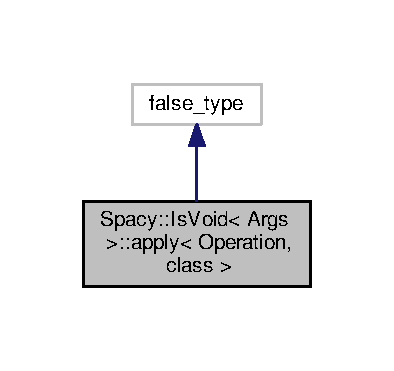
\includegraphics[width=189pt]{structSpacy_1_1IsVoid_1_1apply__inherit__graph}
\end{center}
\end{figure}


Collaboration diagram for Spacy\+:\+:Is\+Void$<$ Args $>$\+:\+:apply$<$ Operation, class $>$\+:
\nopagebreak
\begin{figure}[H]
\begin{center}
\leavevmode
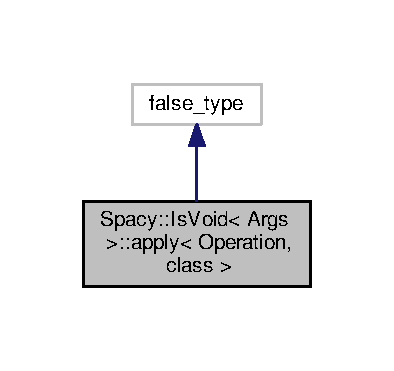
\includegraphics[width=189pt]{structSpacy_1_1IsVoid_1_1apply__coll__graph}
\end{center}
\end{figure}


The documentation for this struct was generated from the following file\+:\begin{DoxyCompactItemize}
\item 
/home/lars/tmp/\+Spacy/\+Spacy/\+Util/voider.\+hh\end{DoxyCompactItemize}

\hypertarget{structSpacy_1_1IsVoid_1_1apply_3_01Operation_00_01void__t_3_01Operation_3_01Args_8_8_8_4_01_4_01_4}{\section{\-Spacy\-:\-:\-Is\-Void$<$ \-Args $>$\-:\-:apply$<$ \-Operation, void\-\_\-t$<$ \-Operation$<$ \-Args...$>$ $>$ $>$ \-Struct \-Template \-Reference}
\label{structSpacy_1_1IsVoid_1_1apply_3_01Operation_00_01void__t_3_01Operation_3_01Args_8_8_8_4_01_4_01_4}\index{\-Spacy\-::\-Is\-Void$<$ Args $>$\-::apply$<$ Operation, void\-\_\-t$<$ Operation$<$ Args...$>$ $>$ $>$@{\-Spacy\-::\-Is\-Void$<$ Args $>$\-::apply$<$ Operation, void\-\_\-t$<$ Operation$<$ Args...$>$ $>$ $>$}}
}
\subsubsection*{template$<$class... \-Args$>$template$<$template$<$ class...$>$ class \-Operation$>$ struct Spacy\-::\-Is\-Void$<$ Args $>$\-::apply$<$ Operation, void\-\_\-t$<$ Operation$<$ Args...$>$ $>$ $>$}



\-The documentation for this struct was generated from the following file\-:\begin{DoxyCompactItemize}
\item 
/home/travis/build/spacy-\/dev/\-Spacy/\-Spacy/\-Util/voider.\-hh\end{DoxyCompactItemize}

\hypertarget{structSpacy_1_1Optional_1_1Mixin_1_1Attach_3_01Mixin_00_01Mixins_8_8_8_4}{\section{\-Spacy\-:\-:\-Optional\-:\-:\-Mixin\-:\-:\-Attach$<$ \-Mixin, \-Mixins...$>$ \-Struct \-Template \-Reference}
\label{structSpacy_1_1Optional_1_1Mixin_1_1Attach_3_01Mixin_00_01Mixins_8_8_8_4}\index{\-Spacy\-::\-Optional\-::\-Mixin\-::\-Attach$<$ Mixin, Mixins...$>$@{\-Spacy\-::\-Optional\-::\-Mixin\-::\-Attach$<$ Mixin, Mixins...$>$}}
}
\subsection*{\-Static \-Public \-Member \-Functions}
\begin{DoxyCompactItemize}
\item 
\hypertarget{structSpacy_1_1Optional_1_1Mixin_1_1Attach_3_01Mixin_00_01Mixins_8_8_8_4_ad894bb9d5fba81bdc5ee4b92b2bd3ea2}{{\footnotesize template$<$class Callee , class To\-Attach , class... \-Other$>$ }\\static void {\bfseries apply} (\-Callee \&callee, \-To\-Attach \&to\-Attach, \-Other \&...other)}\label{structSpacy_1_1Optional_1_1Mixin_1_1Attach_3_01Mixin_00_01Mixins_8_8_8_4_ad894bb9d5fba81bdc5ee4b92b2bd3ea2}

\item 
\hypertarget{structSpacy_1_1Optional_1_1Mixin_1_1Attach_3_01Mixin_00_01Mixins_8_8_8_4_aeea135fae70063c50a7be0d29bbc46d5}{{\footnotesize template$<$class Callee $>$ }\\static void {\bfseries apply} (\-Callee \&)}\label{structSpacy_1_1Optional_1_1Mixin_1_1Attach_3_01Mixin_00_01Mixins_8_8_8_4_aeea135fae70063c50a7be0d29bbc46d5}

\item 
\hypertarget{structSpacy_1_1Optional_1_1Mixin_1_1Attach_3_01Mixin_00_01Mixins_8_8_8_4_a9986fd89deea15e2e3d55272bd4ff1f7}{{\footnotesize template$<$class Callee , class To\-Attach $>$ }\\static void {\bfseries apply} (\-Callee \&callee, \-To\-Attach \&to\-Attach)}\label{structSpacy_1_1Optional_1_1Mixin_1_1Attach_3_01Mixin_00_01Mixins_8_8_8_4_a9986fd89deea15e2e3d55272bd4ff1f7}

\end{DoxyCompactItemize}
\subsubsection*{template$<$class Mixin, class... \-Mixins$>$ struct Spacy\-::\-Optional\-::\-Mixin\-::\-Attach$<$ Mixin, Mixins...$>$}



\-The documentation for this struct was generated from the following file\-:\begin{DoxyCompactItemize}
\item 
/home/travis/build/spacy-\/dev/\-Spacy/\-Spacy/\-Util/\-Mixins/\-Mixin\-Connection.\-hh\end{DoxyCompactItemize}

\hypertarget{structSpacy_1_1Optional_1_1Mixin_1_1Attach_3_4}{\section{Spacy\-:\-:Optional\-:\-:Mixin\-:\-:Attach$<$$>$ Struct Template Reference}
\label{structSpacy_1_1Optional_1_1Mixin_1_1Attach_3_4}\index{Spacy\-::\-Optional\-::\-Mixin\-::\-Attach$<$$>$@{Spacy\-::\-Optional\-::\-Mixin\-::\-Attach$<$$>$}}
}
\subsection*{Static Public Member Functions}
\begin{DoxyCompactItemize}
\item 
\hypertarget{structSpacy_1_1Optional_1_1Mixin_1_1Attach_3_4_ae78568d36f4b9ee4ece2c501880fc894}{{\footnotesize template$<$class Callee , class To\-Attach $>$ }\\static void {\bfseries apply} (Callee \&, To\-Attach \&)}\label{structSpacy_1_1Optional_1_1Mixin_1_1Attach_3_4_ae78568d36f4b9ee4ece2c501880fc894}

\end{DoxyCompactItemize}


The documentation for this struct was generated from the following file\-:\begin{DoxyCompactItemize}
\item 
/home/travis/build/spacy-\/dev/\-Spacy/\-Spacy/\-Util/\-Mixins/Mixin\-Connection.\-hh\end{DoxyCompactItemize}

\hypertarget{structSpacy_1_1ProductSpace_1_1BasicComponentView}{}\section{Spacy\+:\+:Product\+Space\+:\+:Basic\+Component\+View$<$ T $>$ Struct Template Reference}
\label{structSpacy_1_1ProductSpace_1_1BasicComponentView}\index{Spacy\+::\+Product\+Space\+::\+Basic\+Component\+View$<$ T $>$@{Spacy\+::\+Product\+Space\+::\+Basic\+Component\+View$<$ T $>$}}
\subsection*{Public Member Functions}
\begin{DoxyCompactItemize}
\item 
{\bfseries Basic\+Component\+View} (std\+::vector$<$ T $\ast$ $>$ components)\hypertarget{structSpacy_1_1ProductSpace_1_1BasicComponentView_a00b63d0532ba0c10157f655cb010d66f}{}\label{structSpacy_1_1ProductSpace_1_1BasicComponentView_a00b63d0532ba0c10157f655cb010d66f}

\item 
T \& {\bfseries operator\mbox{[}$\,$\mbox{]}} (unsigned k)\hypertarget{structSpacy_1_1ProductSpace_1_1BasicComponentView_a4c95c8eb67ae959ddb718076760d96c5}{}\label{structSpacy_1_1ProductSpace_1_1BasicComponentView_a4c95c8eb67ae959ddb718076760d96c5}

\item 
const T \& {\bfseries operator\mbox{[}$\,$\mbox{]}} (unsigned k) const \hypertarget{structSpacy_1_1ProductSpace_1_1BasicComponentView_ac5b900dd6b8e445581c2b51c0242c95c}{}\label{structSpacy_1_1ProductSpace_1_1BasicComponentView_ac5b900dd6b8e445581c2b51c0242c95c}

\end{DoxyCompactItemize}


The documentation for this struct was generated from the following file\+:\begin{DoxyCompactItemize}
\item 
/home/lars/tmp/\+Spacy/\+Spacy/\+Spaces/\+Product\+Space/vector.\+hh\end{DoxyCompactItemize}

\hypertarget{structSpacy_1_1ProductSpace_1_1BasicComponentView_3_01const_01T_01_4}{\section{\-Spacy\-:\-:\-Product\-Space\-:\-:\-Basic\-Component\-View$<$ const \-T $>$ \-Struct \-Template \-Reference}
\label{structSpacy_1_1ProductSpace_1_1BasicComponentView_3_01const_01T_01_4}\index{\-Spacy\-::\-Product\-Space\-::\-Basic\-Component\-View$<$ const T $>$@{\-Spacy\-::\-Product\-Space\-::\-Basic\-Component\-View$<$ const T $>$}}
}
\subsection*{\-Public \-Member \-Functions}
\begin{DoxyCompactItemize}
\item 
\hypertarget{structSpacy_1_1ProductSpace_1_1BasicComponentView_3_01const_01T_01_4_a52bd2d3c9fd74bd33998586a0e18899b}{{\bfseries \-Basic\-Component\-View} (std\-::vector$<$ const \-T $\ast$ $>$ components)}\label{structSpacy_1_1ProductSpace_1_1BasicComponentView_3_01const_01T_01_4_a52bd2d3c9fd74bd33998586a0e18899b}

\item 
\hypertarget{structSpacy_1_1ProductSpace_1_1BasicComponentView_3_01const_01T_01_4_a1b6db224f3a762bae833aadc0898cda5}{const \-T \& {\bfseries operator\mbox{[}$\,$\mbox{]}} (unsigned k) const }\label{structSpacy_1_1ProductSpace_1_1BasicComponentView_3_01const_01T_01_4_a1b6db224f3a762bae833aadc0898cda5}

\end{DoxyCompactItemize}
\subsubsection*{template$<$class T$>$ struct Spacy\-::\-Product\-Space\-::\-Basic\-Component\-View$<$ const T $>$}



\-The documentation for this struct was generated from the following file\-:\begin{DoxyCompactItemize}
\item 
/home/travis/build/spacy-\/dev/\-Spacy/\-Spacy/\-Spaces/\-Product\-Space/vector.\-hh\end{DoxyCompactItemize}

\hypertarget{classSpacy_1_1C1Functional}{\section{\-Spacy\-:\-:\-C1\-Functional \-Class \-Reference}
\label{classSpacy_1_1C1Functional}\index{\-Spacy\-::\-C1\-Functional@{\-Spacy\-::\-C1\-Functional}}
}


\-Type-\/erased differentiable functional $f:\ X \to \mathbb{R} $.  




{\ttfamily \#include $<$c1\-Functional.\-hh$>$}

\subsection*{\-Public \-Member \-Functions}
\begin{DoxyCompactItemize}
\item 
\hypertarget{classSpacy_1_1C1Functional_a621b710f0c8c583d074f4bf4da3cbb09}{\hyperlink{classSpacy_1_1Real}{\-Real} \hyperlink{classSpacy_1_1C1Functional_a621b710f0c8c583d074f4bf4da3cbb09}{operator()} (const \hyperlink{classSpacy_1_1Vector}{\-Vector} \&x) const }\label{classSpacy_1_1C1Functional_a621b710f0c8c583d074f4bf4da3cbb09}

\begin{DoxyCompactList}\small\item\em \-Apply functional. \end{DoxyCompactList}\item 
\hypertarget{classSpacy_1_1C1Functional_a5953291c58bf20e87ab2bfe26231fe49}{\hyperlink{classSpacy_1_1Vector}{\-Vector} \hyperlink{classSpacy_1_1C1Functional_a5953291c58bf20e87ab2bfe26231fe49}{d1} (const \hyperlink{classSpacy_1_1Vector}{\-Vector} \&x) const }\label{classSpacy_1_1C1Functional_a5953291c58bf20e87ab2bfe26231fe49}

\begin{DoxyCompactList}\small\item\em \-Compute derivative as function space element in $X^*$, where $x\in X$. \end{DoxyCompactList}\item 
\hypertarget{classSpacy_1_1C1Functional_a3ec8df7e7998b557445c907cbd8e80b8}{const \hyperlink{classSpacy_1_1VectorSpace}{\-Vector\-Space} \& \hyperlink{classSpacy_1_1C1Functional_a3ec8df7e7998b557445c907cbd8e80b8}{domain} () const }\label{classSpacy_1_1C1Functional_a3ec8df7e7998b557445c907cbd8e80b8}

\begin{DoxyCompactList}\small\item\em \-Access domain space $X$. \end{DoxyCompactList}\item 
\hypertarget{classSpacy_1_1C1Functional_ada8999210df700c93ee7d7c35bdabebc}{{\footnotesize template$<$typename T , typename std\-::enable\-\_\-if$<$ C1\-Functional\-Detail\-::\-C1\-Functional\-Concept$<$ C1\-Functional, typename std\-::decay$<$ T $>$\-::type $>$\-::value $>$\-::type $\ast$  = nullptr$>$ }\\{\bfseries \-C1\-Functional} (\-T \&\&value)}\label{classSpacy_1_1C1Functional_ada8999210df700c93ee7d7c35bdabebc}

\item 
\hypertarget{classSpacy_1_1C1Functional_a14837fc6ca91107fb783851a31aaa5e3}{{\bfseries type\-\_\-id\-\_\-} (typeid(typename std\-::decay$<$ \-T $>$\-::type).hash\-\_\-code())}\label{classSpacy_1_1C1Functional_a14837fc6ca91107fb783851a31aaa5e3}

\item 
\hypertarget{classSpacy_1_1C1Functional_a07ae129282ab98fd99126cd81bcd0b30}{{\bfseries impl\-\_\-} (nullptr)}\label{classSpacy_1_1C1Functional_a07ae129282ab98fd99126cd81bcd0b30}

\item 
\hypertarget{classSpacy_1_1C1Functional_a8d21587d3af612977b1d054a1997d813}{{\bfseries \-C1\-Functional} (const \hyperlink{classSpacy_1_1C1Functional}{\-C1\-Functional} \&other)}\label{classSpacy_1_1C1Functional_a8d21587d3af612977b1d054a1997d813}

\item 
\hypertarget{classSpacy_1_1C1Functional_a575dc479928f798cae8ad12285ec7563}{{\bfseries \-C1\-Functional} (\hyperlink{classSpacy_1_1C1Functional}{\-C1\-Functional} \&\&other) noexcept}\label{classSpacy_1_1C1Functional_a575dc479928f798cae8ad12285ec7563}

\item 
\hypertarget{classSpacy_1_1C1Functional_a1a6c4893ea11ebeff6647fc12f8b979d}{{\footnotesize template$<$typename T , typename std\-::enable\-\_\-if$<$ C1\-Functional\-Detail\-::\-C1\-Functional\-Concept$<$ C1\-Functional, typename std\-::decay$<$ T $>$\-::type $>$\-::value $>$\-::type $\ast$  = nullptr$>$ }\\\hyperlink{classSpacy_1_1C1Functional}{\-C1\-Functional} \& {\bfseries operator=} (\-T \&\&value)}\label{classSpacy_1_1C1Functional_a1a6c4893ea11ebeff6647fc12f8b979d}

\item 
\hypertarget{classSpacy_1_1C1Functional_a31c2416c61d514298b7ac06526081dae}{\hyperlink{classSpacy_1_1C1Functional}{\-C1\-Functional} \& {\bfseries operator=} (const \hyperlink{classSpacy_1_1C1Functional}{\-C1\-Functional} \&other)}\label{classSpacy_1_1C1Functional_a31c2416c61d514298b7ac06526081dae}

\item 
\hypertarget{classSpacy_1_1C1Functional_a3777c18d812c550efa28d866e5c196e1}{\hyperlink{classSpacy_1_1C1Functional}{\-C1\-Functional} \& {\bfseries operator=} (\hyperlink{classSpacy_1_1C1Functional}{\-C1\-Functional} \&\&other) noexcept}\label{classSpacy_1_1C1Functional_a3777c18d812c550efa28d866e5c196e1}

\item 
\hyperlink{classSpacy_1_1C1Functional_a0b5ae1057d50803d71c7e221424e1ed4}{operator bool} () const noexcept
\begin{DoxyCompactList}\small\item\em \-Checks if the type-\/erased interface holds an implementation. \end{DoxyCompactList}\item 
\hypertarget{classSpacy_1_1C1Functional_a621b710f0c8c583d074f4bf4da3cbb09}{\hyperlink{classSpacy_1_1Real}{\-Real} \hyperlink{classSpacy_1_1C1Functional_a621b710f0c8c583d074f4bf4da3cbb09}{operator()} (const \hyperlink{classSpacy_1_1Vector}{\-Vector} \&x) const }\label{classSpacy_1_1C1Functional_a621b710f0c8c583d074f4bf4da3cbb09}

\begin{DoxyCompactList}\small\item\em \-Apply functional. \end{DoxyCompactList}\item 
\hypertarget{classSpacy_1_1C1Functional_a5953291c58bf20e87ab2bfe26231fe49}{\hyperlink{classSpacy_1_1Vector}{\-Vector} \hyperlink{classSpacy_1_1C1Functional_a5953291c58bf20e87ab2bfe26231fe49}{d1} (const \hyperlink{classSpacy_1_1Vector}{\-Vector} \&x) const }\label{classSpacy_1_1C1Functional_a5953291c58bf20e87ab2bfe26231fe49}

\begin{DoxyCompactList}\small\item\em \-Compute derivative as function space element in $X^*$, where $x\in X$. \end{DoxyCompactList}\item 
\hypertarget{classSpacy_1_1C1Functional_a3ec8df7e7998b557445c907cbd8e80b8}{const \hyperlink{classSpacy_1_1VectorSpace}{\-Vector\-Space} \& \hyperlink{classSpacy_1_1C1Functional_a3ec8df7e7998b557445c907cbd8e80b8}{domain} () const }\label{classSpacy_1_1C1Functional_a3ec8df7e7998b557445c907cbd8e80b8}

\begin{DoxyCompactList}\small\item\em \-Access domain space $X$. \end{DoxyCompactList}\item 
{\footnotesize template$<$class T $>$ }\\\-T $\ast$ \hyperlink{classSpacy_1_1C1Functional_adf7c0fc5a81009ebf4f8c5d9bdb9ec98}{target} () noexcept
\begin{DoxyCompactList}\small\item\em \-Conversion of the stored implementation to. \end{DoxyCompactList}\item 
{\footnotesize template$<$class T $>$ }\\const \-T $\ast$ \hyperlink{classSpacy_1_1C1Functional_aa016d1671e43b875064cf3d9d9bb6351}{target} () const noexcept
\begin{DoxyCompactList}\small\item\em \-Conversion of the stored implementation to. \end{DoxyCompactList}\end{DoxyCompactItemize}


\subsection{\-Detailed \-Description}
\-Type-\/erased differentiable functional $f:\ X \to \mathbb{R} $. 

\subsection{\-Member \-Function \-Documentation}
\hypertarget{classSpacy_1_1C1Functional_a0b5ae1057d50803d71c7e221424e1ed4}{\index{\-Spacy\-::\-C1\-Functional@{\-Spacy\-::\-C1\-Functional}!operator bool@{operator bool}}
\index{operator bool@{operator bool}!Spacy::C1Functional@{\-Spacy\-::\-C1\-Functional}}
\subsubsection[{operator bool}]{\setlength{\rightskip}{0pt plus 5cm}\-Spacy\-::\-C1\-Functional\-::operator bool (
\begin{DoxyParamCaption}
{}
\end{DoxyParamCaption}
) const\hspace{0.3cm}{\ttfamily  \mbox{[}explicit\mbox{]}}}}\label{classSpacy_1_1C1Functional_a0b5ae1057d50803d71c7e221424e1ed4}


\-Checks if the type-\/erased interface holds an implementation. 

\begin{DoxyReturn}{\-Returns}
true if an implementation is stored, else false 
\end{DoxyReturn}
\hypertarget{classSpacy_1_1C1Functional_adf7c0fc5a81009ebf4f8c5d9bdb9ec98}{\index{\-Spacy\-::\-C1\-Functional@{\-Spacy\-::\-C1\-Functional}!target@{target}}
\index{target@{target}!Spacy::C1Functional@{\-Spacy\-::\-C1\-Functional}}
\subsubsection[{target}]{\setlength{\rightskip}{0pt plus 5cm}template$<$class T $>$ \-T$\ast$ {\bf \-Spacy\-::\-C1\-Functional\-::target} (
\begin{DoxyParamCaption}
{}
\end{DoxyParamCaption}
)\hspace{0.3cm}{\ttfamily  \mbox{[}inline\mbox{]}}}}\label{classSpacy_1_1C1Functional_adf7c0fc5a81009ebf4f8c5d9bdb9ec98}


\-Conversion of the stored implementation to. 


\begin{DoxyCode}
 T* 
\end{DoxyCode}
. \begin{DoxyReturn}{\-Returns}
pointer to the stored object if conversion was successful, else nullptr 
\end{DoxyReturn}
\hypertarget{classSpacy_1_1C1Functional_aa016d1671e43b875064cf3d9d9bb6351}{\index{\-Spacy\-::\-C1\-Functional@{\-Spacy\-::\-C1\-Functional}!target@{target}}
\index{target@{target}!Spacy::C1Functional@{\-Spacy\-::\-C1\-Functional}}
\subsubsection[{target}]{\setlength{\rightskip}{0pt plus 5cm}template$<$class T $>$ const \-T$\ast$ {\bf \-Spacy\-::\-C1\-Functional\-::target} (
\begin{DoxyParamCaption}
{}
\end{DoxyParamCaption}
) const\hspace{0.3cm}{\ttfamily  \mbox{[}inline\mbox{]}}}}\label{classSpacy_1_1C1Functional_aa016d1671e43b875064cf3d9d9bb6351}


\-Conversion of the stored implementation to. 


\begin{DoxyCode}
 const T* 
\end{DoxyCode}
. \begin{DoxyReturn}{\-Returns}
pointer to the stored object if conversion was successful, else nullptr 
\end{DoxyReturn}


\-The documentation for this class was generated from the following files\-:\begin{DoxyCompactItemize}
\item 
/home/travis/build/spacy-\/dev/\-Spacy/\-Interfaces/c1\-Functional.\-hh\item 
/home/travis/build/spacy-\/dev/\-Spacy/\-Spacy/c1\-Functional.\-hh\end{DoxyCompactItemize}

\hypertarget{structSpacy_1_1C1FunctionalDetail_1_1C1FunctionalConcept}{\section{\-Spacy\-:\-:\-C1\-Functional\-Detail\-:\-:\-C1\-Functional\-Concept$<$ \-Impl, \-T, bool $>$ \-Struct \-Template \-Reference}
\label{structSpacy_1_1C1FunctionalDetail_1_1C1FunctionalConcept}\index{\-Spacy\-::\-C1\-Functional\-Detail\-::\-C1\-Functional\-Concept$<$ Impl, T, bool $>$@{\-Spacy\-::\-C1\-Functional\-Detail\-::\-C1\-Functional\-Concept$<$ Impl, T, bool $>$}}
}
\subsubsection*{template$<$class Impl, class T, bool = std\-::is\-\_\-same$<$ Impl, T $>$\-::value$>$ struct Spacy\-::\-C1\-Functional\-Detail\-::\-C1\-Functional\-Concept$<$ Impl, T, bool $>$}



\-The documentation for this struct was generated from the following file\-:\begin{DoxyCompactItemize}
\item 
/home/travis/build/spacy-\/dev/\-Spacy/\-Spacy/\-Detail/details\-\_\-for\-\_\-c1\-Functional.\-hh\end{DoxyCompactItemize}

\hypertarget{structSpacy_1_1C1FunctionalDetail_1_1C1FunctionalConcept_3_01Impl_00_01T_00_01false_01_4}{\section{\-Spacy\-:\-:\-C1\-Functional\-Detail\-:\-:\-C1\-Functional\-Concept$<$ \-Impl, \-T, false $>$ \-Struct \-Template \-Reference}
\label{structSpacy_1_1C1FunctionalDetail_1_1C1FunctionalConcept_3_01Impl_00_01T_00_01false_01_4}\index{\-Spacy\-::\-C1\-Functional\-Detail\-::\-C1\-Functional\-Concept$<$ Impl, T, false $>$@{\-Spacy\-::\-C1\-Functional\-Detail\-::\-C1\-Functional\-Concept$<$ Impl, T, false $>$}}
}


\-Inheritance diagram for \-Spacy\-:\-:\-C1\-Functional\-Detail\-:\-:\-C1\-Functional\-Concept$<$ \-Impl, \-T, false $>$\-:
\nopagebreak
\begin{figure}[H]
\begin{center}
\leavevmode
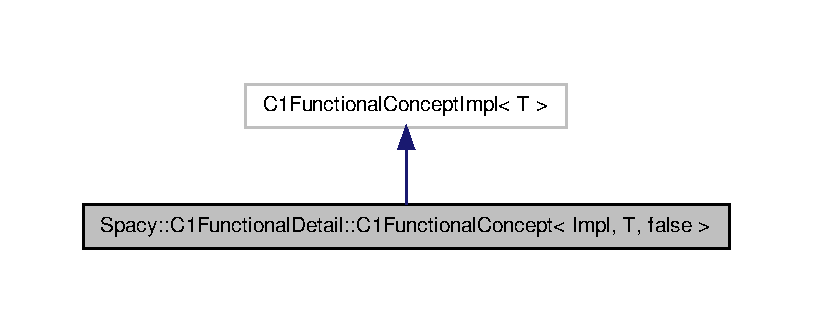
\includegraphics[width=350pt]{structSpacy_1_1C1FunctionalDetail_1_1C1FunctionalConcept_3_01Impl_00_01T_00_01false_01_4__inherit__graph}
\end{center}
\end{figure}


\-Collaboration diagram for \-Spacy\-:\-:\-C1\-Functional\-Detail\-:\-:\-C1\-Functional\-Concept$<$ \-Impl, \-T, false $>$\-:
\nopagebreak
\begin{figure}[H]
\begin{center}
\leavevmode
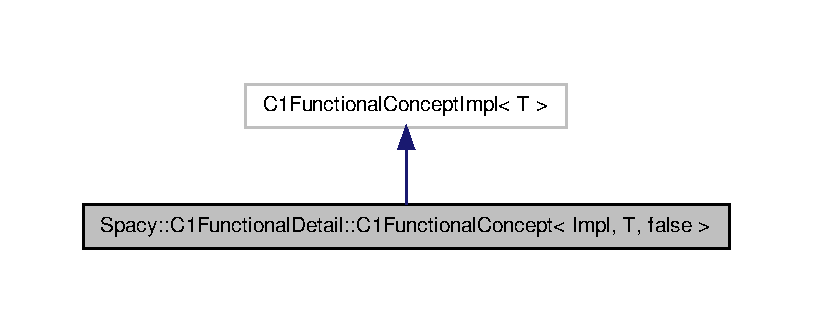
\includegraphics[width=350pt]{structSpacy_1_1C1FunctionalDetail_1_1C1FunctionalConcept_3_01Impl_00_01T_00_01false_01_4__coll__graph}
\end{center}
\end{figure}
\subsubsection*{template$<$class Impl, class T$>$ struct Spacy\-::\-C1\-Functional\-Detail\-::\-C1\-Functional\-Concept$<$ Impl, T, false $>$}



\-The documentation for this struct was generated from the following file\-:\begin{DoxyCompactItemize}
\item 
/home/travis/build/spacy-\/dev/\-Spacy/\-Spacy/\-Detail/details\-\_\-for\-\_\-c1\-Functional.\-hh\end{DoxyCompactItemize}

\hypertarget{classSpacy_1_1Kaskade_1_1C1Operator}{\section{\-Spacy\-:\-:\-Kaskade\-:\-:\-C1\-Operator$<$ \-Operator\-Definition $>$ \-Class \-Template \-Reference}
\label{classSpacy_1_1Kaskade_1_1C1Operator}\index{\-Spacy\-::\-Kaskade\-::\-C1\-Operator$<$ Operator\-Definition $>$@{\-Spacy\-::\-Kaskade\-::\-C1\-Operator$<$ Operator\-Definition $>$}}
}


\-Operator interface for \-Kaskade 7. \-Models a differentiable operator $A:X\rightarrow Y$.  




{\ttfamily \#include $<$c1\-Operator.\-hh$>$}



\-Inheritance diagram for \-Spacy\-:\-:\-Kaskade\-:\-:\-C1\-Operator$<$ \-Operator\-Definition $>$\-:
\nopagebreak
\begin{figure}[H]
\begin{center}
\leavevmode
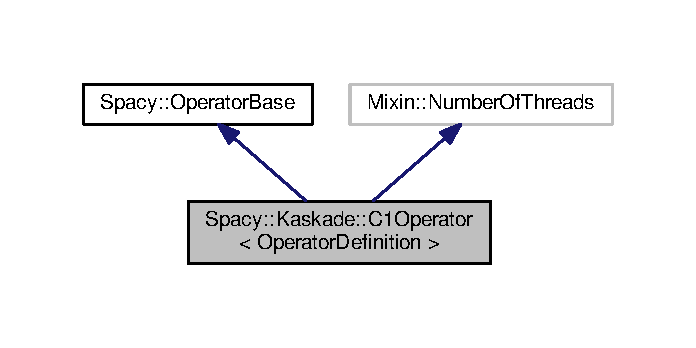
\includegraphics[width=322pt]{classSpacy_1_1Kaskade_1_1C1Operator__inherit__graph}
\end{center}
\end{figure}


\-Collaboration diagram for \-Spacy\-:\-:\-Kaskade\-:\-:\-C1\-Operator$<$ \-Operator\-Definition $>$\-:
\nopagebreak
\begin{figure}[H]
\begin{center}
\leavevmode
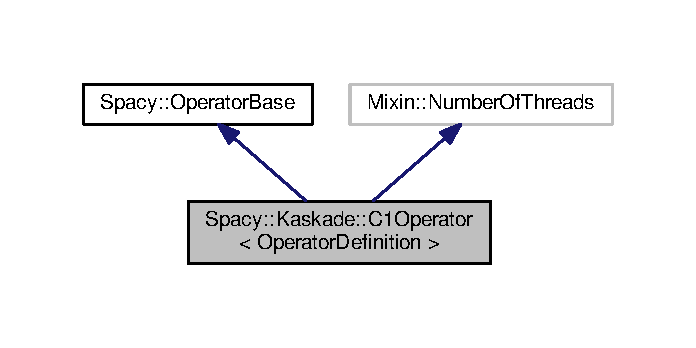
\includegraphics[width=322pt]{classSpacy_1_1Kaskade_1_1C1Operator__coll__graph}
\end{center}
\end{figure}
\subsection*{\-Public \-Member \-Functions}
\begin{DoxyCompactItemize}
\item 
\hyperlink{classSpacy_1_1Kaskade_1_1C1Operator_aa31e9f54fcbb4eb6c40c1cd467d25836}{\-C1\-Operator} (const \-Operator\-Definition \&f, const \hyperlink{classSpacy_1_1VectorSpace}{\-Vector\-Space} \&\hyperlink{classSpacy_1_1OperatorBase_a2588f9b3e0188820c4c494e63293dc6f}{domain}, const \hyperlink{classSpacy_1_1VectorSpace}{\-Vector\-Space} \&\hyperlink{classSpacy_1_1OperatorBase_ab19d3b7a6f290b1079248f1e567e53d6}{range}, int rbegin=0, int rend=\-Operator\-Definition\-::\-Ansatz\-Vars\-::no\-Of\-Variables, int cbegin=0, int cend=\-Operator\-Definition\-::\-Test\-Vars\-::no\-Of\-Variables)
\begin{DoxyCompactList}\small\item\em \-Construct operator for \-Kaskade 7. \end{DoxyCompactList}\item 
\hypertarget{classSpacy_1_1Kaskade_1_1C1Operator_ae3e41254f9aa1362559472ec8335c630}{{\bfseries \-Number\-Of\-Threads} (\-B)}\label{classSpacy_1_1Kaskade_1_1C1Operator_ae3e41254f9aa1362559472ec8335c630}

\item 
\hypertarget{classSpacy_1_1Kaskade_1_1C1Operator_ad00c8f06ca3fa6a5b9a3bef10d05cb5e}{{\bfseries f\-\_\-} (\-B.\-f\-\_\-)}\label{classSpacy_1_1Kaskade_1_1C1Operator_ad00c8f06ca3fa6a5b9a3bef10d05cb5e}

\item 
\hypertarget{classSpacy_1_1Kaskade_1_1C1Operator_a385533b1eff2a7d87962249587d07db9}{{\bfseries spaces\-\_\-} (\-B.\-spaces\-\_\-)}\label{classSpacy_1_1Kaskade_1_1C1Operator_a385533b1eff2a7d87962249587d07db9}

\item 
\hypertarget{classSpacy_1_1Kaskade_1_1C1Operator_a17ca470a8d5dc19211e290a924ce2750}{{\bfseries \-A\-\_\-} (\-B.\-A\-\_\-)}\label{classSpacy_1_1Kaskade_1_1C1Operator_a17ca470a8d5dc19211e290a924ce2750}

\item 
\hypertarget{classSpacy_1_1Kaskade_1_1C1Operator_a60e772d90f9a1546aa9d196fa93459d6}{{\bfseries rhs\-\_\-} (\-B.\-rhs\-\_\-)}\label{classSpacy_1_1Kaskade_1_1C1Operator_a60e772d90f9a1546aa9d196fa93459d6}

\item 
\hypertarget{classSpacy_1_1Kaskade_1_1C1Operator_ab5f1bb2cf0f05f6102520fba0798c985}{{\bfseries old\-\_\-\-X\-\_\-\-A\-\_\-} (\-B.\-old\-\_\-\-X\-\_\-\-A\-\_\-)}\label{classSpacy_1_1Kaskade_1_1C1Operator_ab5f1bb2cf0f05f6102520fba0798c985}

\item 
\hypertarget{classSpacy_1_1Kaskade_1_1C1Operator_a42aa8a24a1da6c875cdd947b6de52687}{{\bfseries old\-\_\-\-X\-\_\-d\-A\-\_\-} (\-B.\-old\-\_\-\-X\-\_\-d\-A\-\_\-)}\label{classSpacy_1_1Kaskade_1_1C1Operator_a42aa8a24a1da6c875cdd947b6de52687}

\item 
\hypertarget{classSpacy_1_1Kaskade_1_1C1Operator_a0014b5685ca7d213e5290d42edd7ef2e}{{\bfseries only\-Lower\-Triangle\-\_\-} (\-B.\-only\-Lower\-Triangle\-\_\-)}\label{classSpacy_1_1Kaskade_1_1C1Operator_a0014b5685ca7d213e5290d42edd7ef2e}

\item 
\hypertarget{classSpacy_1_1Kaskade_1_1C1Operator_a0fe0a5b4fb2e66273145d973112eb417}{{\bfseries rbegin\-\_\-} (\-B.\-rbegin\-\_\-)}\label{classSpacy_1_1Kaskade_1_1C1Operator_a0fe0a5b4fb2e66273145d973112eb417}

\item 
\hypertarget{classSpacy_1_1Kaskade_1_1C1Operator_ac01c1c0351dc6f235cf4dfcac52a6184}{{\bfseries rend\-\_\-} (\-B.\-rend\-\_\-)}\label{classSpacy_1_1Kaskade_1_1C1Operator_ac01c1c0351dc6f235cf4dfcac52a6184}

\item 
\hypertarget{classSpacy_1_1Kaskade_1_1C1Operator_ad9cbbea5b0b57a6eb0dc3f3c4e19cde0}{{\bfseries cbegin\-\_\-} (\-B.\-cbegin\-\_\-)}\label{classSpacy_1_1Kaskade_1_1C1Operator_ad9cbbea5b0b57a6eb0dc3f3c4e19cde0}

\item 
\hypertarget{classSpacy_1_1Kaskade_1_1C1Operator_aedfd011ff833cb84726652752d3b5189}{{\bfseries cend\-\_\-} (\-B.\-cend\-\_\-)}\label{classSpacy_1_1Kaskade_1_1C1Operator_aedfd011ff833cb84726652752d3b5189}

\item 
\hypertarget{classSpacy_1_1Kaskade_1_1C1Operator_a5ef3972f104feec5f10bf3fbf6998f10}{{\bfseries solver\-Creator\-\_\-} (\-B.\-solver\-Creator\-\_\-)}\label{classSpacy_1_1Kaskade_1_1C1Operator_a5ef3972f104feec5f10bf3fbf6998f10}

\item 
\hypertarget{classSpacy_1_1Kaskade_1_1C1Operator_a4d1dc68857b8fd33866d4d0d1bf86473}{{\bfseries operator\-Space\-\_\-} (\-B.\-operator\-Space\-\_\-)}\label{classSpacy_1_1Kaskade_1_1C1Operator_a4d1dc68857b8fd33866d4d0d1bf86473}

\item 
\hyperlink{classSpacy_1_1Kaskade_1_1C1Operator}{\-C1\-Operator} \& \hyperlink{classSpacy_1_1Kaskade_1_1C1Operator_ac378b7b319e5160a7ac19a3697b4291a}{operator=} (const \hyperlink{classSpacy_1_1Kaskade_1_1C1Operator}{\-C1\-Operator} \&\-B)
\begin{DoxyCompactList}\small\item\em \-Copy assignment. \end{DoxyCompactList}\item 
\hyperlink{classSpacy_1_1Kaskade_1_1C1Operator_af75af5b5ee04c86a776d52bc8176d56e}{\-C1\-Operator} (\hyperlink{classSpacy_1_1Kaskade_1_1C1Operator}{\-C1\-Operator} \&\&\-B)
\begin{DoxyCompactList}\small\item\em \-Move constructor. \end{DoxyCompactList}\item 
\hyperlink{classSpacy_1_1Kaskade_1_1C1Operator}{\-C1\-Operator} \& \hyperlink{classSpacy_1_1Kaskade_1_1C1Operator_a99a3c4fc63c5d72285021376c6e57b64}{operator=} (\hyperlink{classSpacy_1_1Kaskade_1_1C1Operator}{\-C1\-Operator} \&\&\-B)
\begin{DoxyCompactList}\small\item\em \-Move assignment. \end{DoxyCompactList}\item 
\-::\hyperlink{classSpacy_1_1Vector}{\-Spacy\-::\-Vector} \hyperlink{classSpacy_1_1Kaskade_1_1C1Operator_aae23a007cd7a66f90bbb1c93da34735d}{operator()} (const \-::\hyperlink{classSpacy_1_1Vector}{\-Spacy\-::\-Vector} \&x) const 
\begin{DoxyCompactList}\small\item\em \-Apply operator. \end{DoxyCompactList}\item 
\-::\hyperlink{classSpacy_1_1Vector}{\-Spacy\-::\-Vector} \hyperlink{classSpacy_1_1Kaskade_1_1C1Operator_a32cfd05c372cc4bc8d7e0e8aedc1e8b9}{d1} (const \-::\hyperlink{classSpacy_1_1Vector}{\-Spacy\-::\-Vector} \&x, const \-::\hyperlink{classSpacy_1_1Vector}{\-Spacy\-::\-Vector} \&dx) const 
\begin{DoxyCompactList}\small\item\em \-Compute $A'(x)dx$. \end{DoxyCompactList}\item 
\hypertarget{classSpacy_1_1Kaskade_1_1C1Operator_afb9837bb1c40e00b53e7430c745b1931}{auto \hyperlink{classSpacy_1_1Kaskade_1_1C1Operator_afb9837bb1c40e00b53e7430c745b1931}{linearization} (const \-::\hyperlink{classSpacy_1_1Vector}{\-Spacy\-::\-Vector} \&x) const }\label{classSpacy_1_1Kaskade_1_1C1Operator_afb9837bb1c40e00b53e7430c745b1931}

\begin{DoxyCompactList}\small\item\em \-Access $A'(x)$ as linear operator $X\rightarrow Y$. \end{DoxyCompactList}\item 
\hypertarget{classSpacy_1_1Kaskade_1_1C1Operator_ab050915a62f3f8bf25e78af1e1289cb8}{const \-Kaskade\-Operator \& \hyperlink{classSpacy_1_1Kaskade_1_1C1Operator_ab050915a62f3f8bf25e78af1e1289cb8}{\-A} () const noexcept}\label{classSpacy_1_1Kaskade_1_1C1Operator_ab050915a62f3f8bf25e78af1e1289cb8}

\begin{DoxyCompactList}\small\item\em \-Access operator representing $A'(x)$. \end{DoxyCompactList}\item 
bool \hyperlink{classSpacy_1_1Kaskade_1_1C1Operator_adb85b50e1cc87fb342412560353c2f73}{only\-Lower\-Triangle} () const noexcept
\begin{DoxyCompactList}\small\item\em \-Access only\-Lower\-Triangle flag. \end{DoxyCompactList}\item 
void \hyperlink{classSpacy_1_1Kaskade_1_1C1Operator_aa0c69955542db6b0f61807181874b4d9}{set\-Solver\-Creator} (std\-::function$<$ \-Linear\-Solver(const \-Linearization \&)$>$ f)
\begin{DoxyCompactList}\small\item\em \-Change solver creator. \end{DoxyCompactList}\item 
\hypertarget{classSpacy_1_1OperatorBase_a2588f9b3e0188820c4c494e63293dc6f}{const \hyperlink{classSpacy_1_1VectorSpace}{\-Vector\-Space} \& \hyperlink{classSpacy_1_1OperatorBase_a2588f9b3e0188820c4c494e63293dc6f}{domain} () const }\label{classSpacy_1_1OperatorBase_a2588f9b3e0188820c4c494e63293dc6f}

\begin{DoxyCompactList}\small\item\em \-Access domain space $X$. \end{DoxyCompactList}\item 
\hypertarget{classSpacy_1_1OperatorBase_ab19d3b7a6f290b1079248f1e567e53d6}{const \hyperlink{classSpacy_1_1VectorSpace}{\-Vector\-Space} \& \hyperlink{classSpacy_1_1OperatorBase_ab19d3b7a6f290b1079248f1e567e53d6}{range} () const }\label{classSpacy_1_1OperatorBase_ab19d3b7a6f290b1079248f1e567e53d6}

\begin{DoxyCompactList}\small\item\em \-Access range space $Y$. \end{DoxyCompactList}\end{DoxyCompactItemize}


\subsection{\-Detailed \-Description}
\subsubsection*{template$<$class \-Operator\-Definition$>$class Spacy\-::\-Kaskade\-::\-C1\-Operator$<$ Operator\-Definition $>$}

\-Operator interface for \-Kaskade 7. \-Models a differentiable operator $A:X\rightarrow Y$. 

\begin{DoxySeeAlso}{\-See also}
\hyperlink{classSpacy_1_1C1Operator}{\-Spacy\-::\-C1\-Operator} 
\end{DoxySeeAlso}


\subsection{\-Constructor \& \-Destructor \-Documentation}
\hypertarget{classSpacy_1_1Kaskade_1_1C1Operator_aa31e9f54fcbb4eb6c40c1cd467d25836}{\index{\-Spacy\-::\-Kaskade\-::\-C1\-Operator@{\-Spacy\-::\-Kaskade\-::\-C1\-Operator}!\-C1\-Operator@{\-C1\-Operator}}
\index{\-C1\-Operator@{\-C1\-Operator}!Spacy::Kaskade::C1Operator@{\-Spacy\-::\-Kaskade\-::\-C1\-Operator}}
\subsubsection[{\-C1\-Operator}]{\setlength{\rightskip}{0pt plus 5cm}template$<$class \-Operator\-Definition$>$ {\bf \-Spacy\-::\-Kaskade\-::\-C1\-Operator}$<$ \-Operator\-Definition $>$\-::{\bf \-C1\-Operator} (
\begin{DoxyParamCaption}
\item[{const \-Operator\-Definition \&}]{f, }
\item[{const {\bf \-Vector\-Space} \&}]{domain, }
\item[{const {\bf \-Vector\-Space} \&}]{range, }
\item[{int}]{rbegin = {\ttfamily 0}, }
\item[{int}]{rend = {\ttfamily \-Operator\-Definition\-:\-:\-Ansatz\-Vars\-:\-:no\-Of\-Variables}, }
\item[{int}]{cbegin = {\ttfamily 0}, }
\item[{int}]{cend = {\ttfamily \-Operator\-Definition\-:\-:\-Test\-Vars\-:\-:no\-Of\-Variables}}
\end{DoxyParamCaption}
)\hspace{0.3cm}{\ttfamily  \mbox{[}inline\mbox{]}}}}\label{classSpacy_1_1Kaskade_1_1C1Operator_aa31e9f54fcbb4eb6c40c1cd467d25836}


\-Construct operator for \-Kaskade 7. 


\begin{DoxyParams}{\-Parameters}
{\em f} & operator definition from \-Kaskade 7 \\
\hline
{\em domain} & domain space \\
\hline
{\em range} & range space \\
\hline
{\em rbegin} & first row to be considered in the definition of f \\
\hline
{\em rend} & one after the last row to be considered in the definition of f \\
\hline
{\em cbegin} & first column to be considered in the definition of f \\
\hline
{\em cend} & one after the last column to be considered in the definition of f\\
\hline
\end{DoxyParams}
\-The optional parameters rbegin, rend, cbegin and cend can be used to define operators that correspond to parts of a system of equation. \hypertarget{classSpacy_1_1Kaskade_1_1C1Operator_af75af5b5ee04c86a776d52bc8176d56e}{\index{\-Spacy\-::\-Kaskade\-::\-C1\-Operator@{\-Spacy\-::\-Kaskade\-::\-C1\-Operator}!\-C1\-Operator@{\-C1\-Operator}}
\index{\-C1\-Operator@{\-C1\-Operator}!Spacy::Kaskade::C1Operator@{\-Spacy\-::\-Kaskade\-::\-C1\-Operator}}
\subsubsection[{\-C1\-Operator}]{\setlength{\rightskip}{0pt plus 5cm}template$<$class \-Operator\-Definition$>$ {\bf \-Spacy\-::\-Kaskade\-::\-C1\-Operator}$<$ \-Operator\-Definition $>$\-::{\bf \-C1\-Operator} (
\begin{DoxyParamCaption}
\item[{{\bf \-C1\-Operator}$<$ \-Operator\-Definition $>$ \&\&}]{\-B}
\end{DoxyParamCaption}
)}}\label{classSpacy_1_1Kaskade_1_1C1Operator_af75af5b5ee04c86a776d52bc8176d56e}


\-Move constructor. 


\begin{DoxyParams}{\-Parameters}
{\em \-B} & object to move from \\
\hline
\end{DoxyParams}


\subsection{\-Member \-Function \-Documentation}
\hypertarget{classSpacy_1_1Kaskade_1_1C1Operator_ac378b7b319e5160a7ac19a3697b4291a}{\index{\-Spacy\-::\-Kaskade\-::\-C1\-Operator@{\-Spacy\-::\-Kaskade\-::\-C1\-Operator}!operator=@{operator=}}
\index{operator=@{operator=}!Spacy::Kaskade::C1Operator@{\-Spacy\-::\-Kaskade\-::\-C1\-Operator}}
\subsubsection[{operator=}]{\setlength{\rightskip}{0pt plus 5cm}template$<$class \-Operator\-Definition$>$ {\bf \-C1\-Operator}\& {\bf \-Spacy\-::\-Kaskade\-::\-C1\-Operator}$<$ \-Operator\-Definition $>$\-::operator= (
\begin{DoxyParamCaption}
\item[{const {\bf \-C1\-Operator}$<$ \-Operator\-Definition $>$ \&}]{\-B}
\end{DoxyParamCaption}
)\hspace{0.3cm}{\ttfamily  \mbox{[}inline\mbox{]}}}}\label{classSpacy_1_1Kaskade_1_1C1Operator_ac378b7b319e5160a7ac19a3697b4291a}


\-Copy assignment. 


\begin{DoxyParams}{\-Parameters}
{\em \-B} & object to copy from \\
\hline
\end{DoxyParams}
\hypertarget{classSpacy_1_1Kaskade_1_1C1Operator_a99a3c4fc63c5d72285021376c6e57b64}{\index{\-Spacy\-::\-Kaskade\-::\-C1\-Operator@{\-Spacy\-::\-Kaskade\-::\-C1\-Operator}!operator=@{operator=}}
\index{operator=@{operator=}!Spacy::Kaskade::C1Operator@{\-Spacy\-::\-Kaskade\-::\-C1\-Operator}}
\subsubsection[{operator=}]{\setlength{\rightskip}{0pt plus 5cm}template$<$class \-Operator\-Definition$>$ {\bf \-C1\-Operator}\& {\bf \-Spacy\-::\-Kaskade\-::\-C1\-Operator}$<$ \-Operator\-Definition $>$\-::operator= (
\begin{DoxyParamCaption}
\item[{{\bf \-C1\-Operator}$<$ \-Operator\-Definition $>$ \&\&}]{\-B}
\end{DoxyParamCaption}
)}}\label{classSpacy_1_1Kaskade_1_1C1Operator_a99a3c4fc63c5d72285021376c6e57b64}


\-Move assignment. 


\begin{DoxyParams}{\-Parameters}
{\em \-B} & object to move from \\
\hline
\end{DoxyParams}
\hypertarget{classSpacy_1_1Kaskade_1_1C1Operator_aae23a007cd7a66f90bbb1c93da34735d}{\index{\-Spacy\-::\-Kaskade\-::\-C1\-Operator@{\-Spacy\-::\-Kaskade\-::\-C1\-Operator}!operator()@{operator()}}
\index{operator()@{operator()}!Spacy::Kaskade::C1Operator@{\-Spacy\-::\-Kaskade\-::\-C1\-Operator}}
\subsubsection[{operator()}]{\setlength{\rightskip}{0pt plus 5cm}template$<$class \-Operator\-Definition$>$ \-::{\bf \-Spacy\-::\-Vector} {\bf \-Spacy\-::\-Kaskade\-::\-C1\-Operator}$<$ \-Operator\-Definition $>$\-::operator() (
\begin{DoxyParamCaption}
\item[{const \-::{\bf \-Spacy\-::\-Vector} \&}]{x}
\end{DoxyParamCaption}
) const\hspace{0.3cm}{\ttfamily  \mbox{[}inline\mbox{]}}}}\label{classSpacy_1_1Kaskade_1_1C1Operator_aae23a007cd7a66f90bbb1c93da34735d}


\-Apply operator. 


\begin{DoxyParams}{\-Parameters}
{\em x} & argument \\
\hline
\end{DoxyParams}
\begin{DoxyReturn}{\-Returns}
$A(x)$ 
\end{DoxyReturn}
\hypertarget{classSpacy_1_1Kaskade_1_1C1Operator_a32cfd05c372cc4bc8d7e0e8aedc1e8b9}{\index{\-Spacy\-::\-Kaskade\-::\-C1\-Operator@{\-Spacy\-::\-Kaskade\-::\-C1\-Operator}!d1@{d1}}
\index{d1@{d1}!Spacy::Kaskade::C1Operator@{\-Spacy\-::\-Kaskade\-::\-C1\-Operator}}
\subsubsection[{d1}]{\setlength{\rightskip}{0pt plus 5cm}template$<$class \-Operator\-Definition$>$ \-::{\bf \-Spacy\-::\-Vector} {\bf \-Spacy\-::\-Kaskade\-::\-C1\-Operator}$<$ \-Operator\-Definition $>$\-::{\bf d1} (
\begin{DoxyParamCaption}
\item[{const \-::{\bf \-Spacy\-::\-Vector} \&}]{x, }
\item[{const \-::{\bf \-Spacy\-::\-Vector} \&}]{dx}
\end{DoxyParamCaption}
) const\hspace{0.3cm}{\ttfamily  \mbox{[}inline\mbox{]}}}}\label{classSpacy_1_1Kaskade_1_1C1Operator_a32cfd05c372cc4bc8d7e0e8aedc1e8b9}


\-Compute $A'(x)dx$. 


\begin{DoxyParams}{\-Parameters}
{\em x} & current iterate \\
\hline
{\em dx} & correction \\
\hline
\end{DoxyParams}
\begin{DoxyReturn}{\-Returns}
$A'(x)dx$ 
\end{DoxyReturn}
\hypertarget{classSpacy_1_1Kaskade_1_1C1Operator_adb85b50e1cc87fb342412560353c2f73}{\index{\-Spacy\-::\-Kaskade\-::\-C1\-Operator@{\-Spacy\-::\-Kaskade\-::\-C1\-Operator}!only\-Lower\-Triangle@{only\-Lower\-Triangle}}
\index{only\-Lower\-Triangle@{only\-Lower\-Triangle}!Spacy::Kaskade::C1Operator@{\-Spacy\-::\-Kaskade\-::\-C1\-Operator}}
\subsubsection[{only\-Lower\-Triangle}]{\setlength{\rightskip}{0pt plus 5cm}template$<$class \-Operator\-Definition$>$ bool {\bf \-Spacy\-::\-Kaskade\-::\-C1\-Operator}$<$ \-Operator\-Definition $>$\-::{\bf only\-Lower\-Triangle} (
\begin{DoxyParamCaption}
{}
\end{DoxyParamCaption}
) const\hspace{0.3cm}{\ttfamily  \mbox{[}inline\mbox{]}}}}\label{classSpacy_1_1Kaskade_1_1C1Operator_adb85b50e1cc87fb342412560353c2f73}


\-Access only\-Lower\-Triangle flag. 

\begin{DoxyReturn}{\-Returns}
true if only the lower triangle of a symmetric matrix is stored in the operator definition, else false 
\end{DoxyReturn}
\hypertarget{classSpacy_1_1Kaskade_1_1C1Operator_aa0c69955542db6b0f61807181874b4d9}{\index{\-Spacy\-::\-Kaskade\-::\-C1\-Operator@{\-Spacy\-::\-Kaskade\-::\-C1\-Operator}!set\-Solver\-Creator@{set\-Solver\-Creator}}
\index{set\-Solver\-Creator@{set\-Solver\-Creator}!Spacy::Kaskade::C1Operator@{\-Spacy\-::\-Kaskade\-::\-C1\-Operator}}
\subsubsection[{set\-Solver\-Creator}]{\setlength{\rightskip}{0pt plus 5cm}template$<$class \-Operator\-Definition$>$ void {\bf \-Spacy\-::\-Kaskade\-::\-C1\-Operator}$<$ \-Operator\-Definition $>$\-::{\bf set\-Solver\-Creator} (
\begin{DoxyParamCaption}
\item[{std\-::function$<$ \-Linear\-Solver(const \-Linearization \&)$>$}]{f}
\end{DoxyParamCaption}
)\hspace{0.3cm}{\ttfamily  \mbox{[}inline\mbox{]}}}}\label{classSpacy_1_1Kaskade_1_1C1Operator_aa0c69955542db6b0f61807181874b4d9}


\-Change solver creator. 


\begin{DoxyParams}{\-Parameters}
{\em f} & function/functor for the creation of a linear solver \\
\hline
\end{DoxyParams}


\-The documentation for this class was generated from the following file\-:\begin{DoxyCompactItemize}
\item 
/home/travis/build/spacy-\/dev/\-Spacy/\-Spacy/\-Adapter/\-Kaskade/c1\-Operator.\-hh\end{DoxyCompactItemize}

\hypertarget{classSpacy_1_1Scalar_1_1C1Operator}{\section{Spacy\-:\-:Scalar\-:\-:C1\-Operator Class Reference}
\label{classSpacy_1_1Scalar_1_1C1Operator}\index{Spacy\-::\-Scalar\-::\-C1\-Operator@{Spacy\-::\-Scalar\-::\-C1\-Operator}}
}


Inheritance diagram for Spacy\-:\-:Scalar\-:\-:C1\-Operator\-:
\nopagebreak
\begin{figure}[H]
\begin{center}
\leavevmode
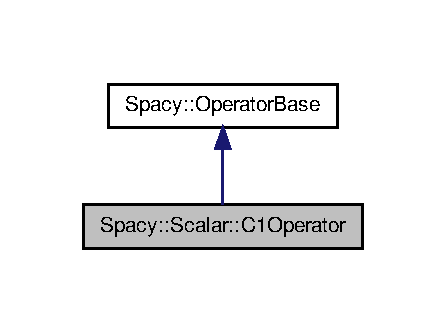
\includegraphics[width=214pt]{classSpacy_1_1Scalar_1_1C1Operator__inherit__graph}
\end{center}
\end{figure}


Collaboration diagram for Spacy\-:\-:Scalar\-:\-:C1\-Operator\-:
\nopagebreak
\begin{figure}[H]
\begin{center}
\leavevmode
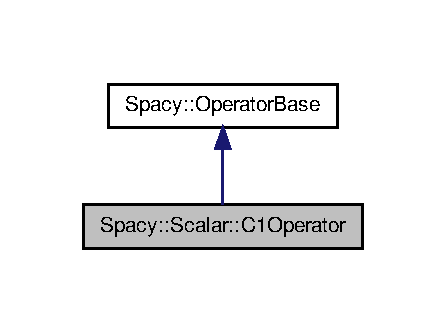
\includegraphics[width=214pt]{classSpacy_1_1Scalar_1_1C1Operator__coll__graph}
\end{center}
\end{figure}
\subsection*{Public Member Functions}
\begin{DoxyCompactItemize}
\item 
\hypertarget{classSpacy_1_1Scalar_1_1C1Operator_a97f719a6349064072c892972663e70c7}{{\bfseries C1\-Operator} (std\-::function$<$ double(double)$>$ value, std\-::function$<$ double(double)$>$ \hyperlink{namespaceSpacy_a002fe344fa6d04a6ac59a74ea25fddb6}{derivative})}\label{classSpacy_1_1Scalar_1_1C1Operator_a97f719a6349064072c892972663e70c7}

\item 
\hypertarget{classSpacy_1_1Scalar_1_1C1Operator_a9ab2d8a905a70dd848c984e532b50fed}{\hyperlink{classSpacy_1_1Vector}{Spacy\-::\-Vector} {\bfseries operator()} (const \-::\hyperlink{classSpacy_1_1Vector}{Spacy\-::\-Vector} \&x) const }\label{classSpacy_1_1Scalar_1_1C1Operator_a9ab2d8a905a70dd848c984e532b50fed}

\item 
\hypertarget{classSpacy_1_1Scalar_1_1C1Operator_a56908ac8a9cd1e959f15e3f71a00a01b}{\hyperlink{classSpacy_1_1Vector}{Spacy\-::\-Vector} {\bfseries d1} (const \-::\hyperlink{classSpacy_1_1Vector}{Spacy\-::\-Vector} \&x, const \-::\hyperlink{classSpacy_1_1Vector}{Spacy\-::\-Vector} \&dx) const }\label{classSpacy_1_1Scalar_1_1C1Operator_a56908ac8a9cd1e959f15e3f71a00a01b}

\item 
\hypertarget{classSpacy_1_1Scalar_1_1C1Operator_acefccd4cac61750dad6053a963b10944}{\hyperlink{structSpacy_1_1Scalar_1_1LinearOperator}{Linear\-Operator} {\bfseries linearization} (const \-::\hyperlink{classSpacy_1_1Vector}{Spacy\-::\-Vector} \&x) const }\label{classSpacy_1_1Scalar_1_1C1Operator_acefccd4cac61750dad6053a963b10944}

\item 
\hypertarget{classSpacy_1_1OperatorBase_a2588f9b3e0188820c4c494e63293dc6f}{const \hyperlink{classSpacy_1_1VectorSpace}{Vector\-Space} \& \hyperlink{classSpacy_1_1OperatorBase_a2588f9b3e0188820c4c494e63293dc6f}{domain} () const }\label{classSpacy_1_1OperatorBase_a2588f9b3e0188820c4c494e63293dc6f}

\begin{DoxyCompactList}\small\item\em Access domain space $X$. \end{DoxyCompactList}\item 
\hypertarget{classSpacy_1_1OperatorBase_ab19d3b7a6f290b1079248f1e567e53d6}{const \hyperlink{classSpacy_1_1VectorSpace}{Vector\-Space} \& \hyperlink{classSpacy_1_1OperatorBase_ab19d3b7a6f290b1079248f1e567e53d6}{range} () const }\label{classSpacy_1_1OperatorBase_ab19d3b7a6f290b1079248f1e567e53d6}

\begin{DoxyCompactList}\small\item\em Access range space $Y$. \end{DoxyCompactList}\end{DoxyCompactItemize}


The documentation for this class was generated from the following file\-:\begin{DoxyCompactItemize}
\item 
/home/travis/build/spacy-\/dev/\-Spacy/\-Spacy/\-Spaces/\-Scalar\-Space/c1\-Operator.\-hh\end{DoxyCompactItemize}

\hypertarget{classSpacy_1_1C1Operator}{\section{Spacy\-:\-:C1\-Operator Class Reference}
\label{classSpacy_1_1C1Operator}\index{Spacy\-::\-C1\-Operator@{Spacy\-::\-C1\-Operator}}
}


Type-\/erased differentiable operator $A:\ X \to Y $.  




{\ttfamily \#include $<$c1\-Operator.\-hh$>$}

\subsection*{Public Member Functions}
\begin{DoxyCompactItemize}
\item 
\hypertarget{classSpacy_1_1C1Operator_a2a01bf08bf2b6e44955cd606aa3db91d}{\hyperlink{classSpacy_1_1Vector}{Vector} \hyperlink{classSpacy_1_1C1Operator_a2a01bf08bf2b6e44955cd606aa3db91d}{operator()} (const \hyperlink{classSpacy_1_1Vector}{Vector} \&x) const }\label{classSpacy_1_1C1Operator_a2a01bf08bf2b6e44955cd606aa3db91d}

\begin{DoxyCompactList}\small\item\em Apply operator. \end{DoxyCompactList}\item 
\hypertarget{classSpacy_1_1C1Operator_a1b6a06c88bc4168c750ee4ffdc81f1dd}{\hyperlink{classSpacy_1_1Vector}{Vector} \hyperlink{classSpacy_1_1C1Operator_a1b6a06c88bc4168c750ee4ffdc81f1dd}{d1} (const \hyperlink{classSpacy_1_1Vector}{Vector} \&x, const \hyperlink{classSpacy_1_1Vector}{Vector} \&dx) const }\label{classSpacy_1_1C1Operator_a1b6a06c88bc4168c750ee4ffdc81f1dd}

\begin{DoxyCompactList}\small\item\em Compute directional derivative $A'(x)\delta x$. \end{DoxyCompactList}\item 
\hypertarget{classSpacy_1_1C1Operator_a71aabe09ec29a8a1bb197eef035d6672}{\hyperlink{classSpacy_1_1LinearOperator}{Linear\-Operator} \hyperlink{classSpacy_1_1C1Operator_a71aabe09ec29a8a1bb197eef035d6672}{linearization} (const \hyperlink{classSpacy_1_1Vector}{Vector} \&x) const }\label{classSpacy_1_1C1Operator_a71aabe09ec29a8a1bb197eef035d6672}

\begin{DoxyCompactList}\small\item\em Get linearization $A'(x):\ X\to Y $. \end{DoxyCompactList}\item 
\hypertarget{classSpacy_1_1C1Operator_aee0ffd5cee0b8a8df2f0b67b5aaf0ddb}{const \hyperlink{classSpacy_1_1VectorSpace}{Vector\-Space} \& \hyperlink{classSpacy_1_1C1Operator_aee0ffd5cee0b8a8df2f0b67b5aaf0ddb}{domain} () const }\label{classSpacy_1_1C1Operator_aee0ffd5cee0b8a8df2f0b67b5aaf0ddb}

\begin{DoxyCompactList}\small\item\em Access domain space $X$. \end{DoxyCompactList}\item 
\hypertarget{classSpacy_1_1C1Operator_a7df27427591907b13776e7ba3707bf05}{const \hyperlink{classSpacy_1_1VectorSpace}{Vector\-Space} \& \hyperlink{classSpacy_1_1C1Operator_a7df27427591907b13776e7ba3707bf05}{range} () const }\label{classSpacy_1_1C1Operator_a7df27427591907b13776e7ba3707bf05}

\begin{DoxyCompactList}\small\item\em Access range space $Y$. \end{DoxyCompactList}\item 
\hypertarget{classSpacy_1_1C1Operator_a9a46e9d2fb4526fa320480b832c5b71e}{{\footnotesize template$<$class T , typename std\-::enable\-\_\-if$<$ C1\-Operator\-Detail\-::\-Concept$<$ C1\-Operator, typename std\-::decay$<$ T $>$\-::type $>$\-::value $>$\-::type $\ast$  = nullptr$>$ }\\{\bfseries C1\-Operator} (T \&\&value)}\label{classSpacy_1_1C1Operator_a9a46e9d2fb4526fa320480b832c5b71e}

\item 
\hypertarget{classSpacy_1_1C1Operator_ae4068d2989e5aa71b372def134afdd78}{{\bfseries impl\-\_\-} (std\-::forward$<$ T $>$(value))}\label{classSpacy_1_1C1Operator_ae4068d2989e5aa71b372def134afdd78}

\item 
\hypertarget{classSpacy_1_1C1Operator_aecfc71bf5da728a9028a586e50afbfcf}{{\footnotesize template$<$class T , typename std\-::enable\-\_\-if$<$ C1\-Operator\-Detail\-::\-Concept$<$ C1\-Operator, typename std\-::decay$<$ T $>$\-::type $>$\-::value $>$\-::type $\ast$  = nullptr$>$ }\\\hyperlink{classSpacy_1_1C1Operator}{C1\-Operator} \& {\bfseries operator=} (T \&\&value)}\label{classSpacy_1_1C1Operator_aecfc71bf5da728a9028a586e50afbfcf}

\item 
\hypertarget{classSpacy_1_1C1Operator_a4efdf099aac5f0b101c69cc8c9c8a48b}{{\bfseries operator bool} () const noexcept}\label{classSpacy_1_1C1Operator_a4efdf099aac5f0b101c69cc8c9c8a48b}

\item 
\hypertarget{classSpacy_1_1C1Operator_a2a01bf08bf2b6e44955cd606aa3db91d}{\hyperlink{classSpacy_1_1Vector}{Vector} \hyperlink{classSpacy_1_1C1Operator_a2a01bf08bf2b6e44955cd606aa3db91d}{operator()} (const \hyperlink{classSpacy_1_1Vector}{Vector} \&x) const }\label{classSpacy_1_1C1Operator_a2a01bf08bf2b6e44955cd606aa3db91d}

\begin{DoxyCompactList}\small\item\em Apply operator. \end{DoxyCompactList}\item 
\hypertarget{classSpacy_1_1C1Operator_a1b6a06c88bc4168c750ee4ffdc81f1dd}{\hyperlink{classSpacy_1_1Vector}{Vector} \hyperlink{classSpacy_1_1C1Operator_a1b6a06c88bc4168c750ee4ffdc81f1dd}{d1} (const \hyperlink{classSpacy_1_1Vector}{Vector} \&x, const \hyperlink{classSpacy_1_1Vector}{Vector} \&dx) const }\label{classSpacy_1_1C1Operator_a1b6a06c88bc4168c750ee4ffdc81f1dd}

\begin{DoxyCompactList}\small\item\em Compute directional derivative $A'(x)\delta x$. \end{DoxyCompactList}\item 
\hypertarget{classSpacy_1_1C1Operator_a71aabe09ec29a8a1bb197eef035d6672}{\hyperlink{classSpacy_1_1LinearOperator}{Linear\-Operator} \hyperlink{classSpacy_1_1C1Operator_a71aabe09ec29a8a1bb197eef035d6672}{linearization} (const \hyperlink{classSpacy_1_1Vector}{Vector} \&x) const }\label{classSpacy_1_1C1Operator_a71aabe09ec29a8a1bb197eef035d6672}

\begin{DoxyCompactList}\small\item\em Get linearization. \end{DoxyCompactList}\item 
\hypertarget{classSpacy_1_1C1Operator_a0ce49bb91eee9fa9cc5d63599ab9b23c}{Access domain space f \$X f \\*
const \hyperlink{classSpacy_1_1VectorSpace}{Vector\-Space} \& {\bfseries domain} () const }\label{classSpacy_1_1C1Operator_a0ce49bb91eee9fa9cc5d63599ab9b23c}

\item 
\hypertarget{classSpacy_1_1C1Operator_a1331de78c1c489b846507c3f7461dc15}{Access range space f \$Y f \\*
const \hyperlink{classSpacy_1_1VectorSpace}{Vector\-Space} \& {\bfseries range} () const }\label{classSpacy_1_1C1Operator_a1331de78c1c489b846507c3f7461dc15}

\item 
\hypertarget{classSpacy_1_1C1Operator_a7c515af344029cf8e60e89d45bf8fade}{{\footnotesize template$<$class T $>$ }\\T $\ast$ {\bfseries target} () noexcept}\label{classSpacy_1_1C1Operator_a7c515af344029cf8e60e89d45bf8fade}

\item 
\hypertarget{classSpacy_1_1C1Operator_ab8a5618949b1b861e3085aa085922884}{{\footnotesize template$<$class T $>$ }\\const T $\ast$ {\bfseries target} () const noexcept}\label{classSpacy_1_1C1Operator_ab8a5618949b1b861e3085aa085922884}

\end{DoxyCompactItemize}


\subsection{Detailed Description}
Type-\/erased differentiable operator $A:\ X \to Y $. 

The documentation for this class was generated from the following file\-:\begin{DoxyCompactItemize}
\item 
/home/travis/build/spacy-\/dev/\-Spacy/\-Interfaces/c1\-Operator.\-hh\end{DoxyCompactItemize}

\hypertarget{classSpacy_1_1Rn_1_1C1Operator}{\section{\-Spacy\-:\-:\-Rn\-:\-:\-C1\-Operator \-Class \-Reference}
\label{classSpacy_1_1Rn_1_1C1Operator}\index{\-Spacy\-::\-Rn\-::\-C1\-Operator@{\-Spacy\-::\-Rn\-::\-C1\-Operator}}
}


\-A differential operator $A:X\rightarrow Y$ for finite-\/dimensional problems, based on the \-Eigen library.  




{\ttfamily \#include $<$c1\-Operator.\-hh$>$}



\-Inheritance diagram for \-Spacy\-:\-:\-Rn\-:\-:\-C1\-Operator\-:
\nopagebreak
\begin{figure}[H]
\begin{center}
\leavevmode
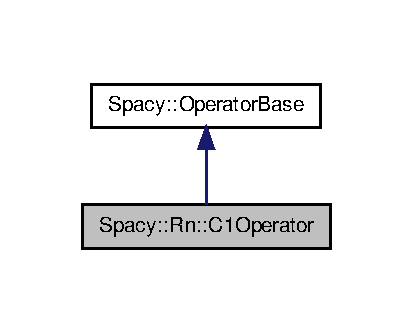
\includegraphics[width=198pt]{classSpacy_1_1Rn_1_1C1Operator__inherit__graph}
\end{center}
\end{figure}


\-Collaboration diagram for \-Spacy\-:\-:\-Rn\-:\-:\-C1\-Operator\-:
\nopagebreak
\begin{figure}[H]
\begin{center}
\leavevmode
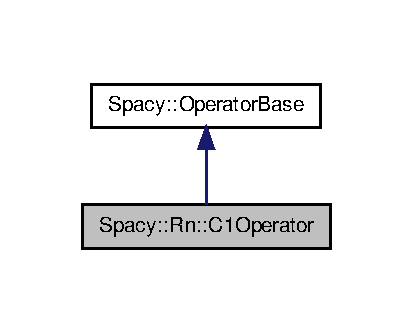
\includegraphics[width=198pt]{classSpacy_1_1Rn_1_1C1Operator__coll__graph}
\end{center}
\end{figure}
\subsection*{\-Public \-Member \-Functions}
\begin{DoxyCompactItemize}
\item 
\hyperlink{classSpacy_1_1Rn_1_1C1Operator_ace713dafa8c7422f57f0f1c0a989db12}{\-C1\-Operator} (std\-::function$<$ \-::\-Eigen\-::\-Vector\-Xd(const \-::\-Eigen\-::\-Vector\-Xd \&) $>$ value, std\-::function$<$ \-::\-Eigen\-::\-Matrix\-Xd(const \-::\-Eigen\-::\-Vector\-Xd \&) $>$ \hyperlink{namespaceSpacy_a002fe344fa6d04a6ac59a74ea25fddb6}{derivative}, const \hyperlink{classSpacy_1_1VectorSpace}{\-Vector\-Space} \&\hyperlink{classSpacy_1_1OperatorBase_a2588f9b3e0188820c4c494e63293dc6f}{domain}, const \hyperlink{classSpacy_1_1VectorSpace}{\-Vector\-Space} \&\hyperlink{classSpacy_1_1OperatorBase_ab19d3b7a6f290b1079248f1e567e53d6}{range})
\begin{DoxyCompactList}\small\item\em \hyperlink{classSpacy_1_1Rn_1_1C1Operator}{\-C1\-Operator}. \end{DoxyCompactList}\item 
\hypertarget{classSpacy_1_1Rn_1_1C1Operator_a21205efc25688cb7d5f184eeb637df60}{\-::\hyperlink{classSpacy_1_1Vector}{\-Spacy\-::\-Vector} \hyperlink{classSpacy_1_1Rn_1_1C1Operator_a21205efc25688cb7d5f184eeb637df60}{operator()} (const \-::\hyperlink{classSpacy_1_1Vector}{\-Spacy\-::\-Vector} \&x) const }\label{classSpacy_1_1Rn_1_1C1Operator_a21205efc25688cb7d5f184eeb637df60}

\begin{DoxyCompactList}\small\item\em \-Compute \-A(x). \end{DoxyCompactList}\item 
\hypertarget{classSpacy_1_1Rn_1_1C1Operator_af15f1491a967262ffcfe6d484d440940}{\-::\hyperlink{classSpacy_1_1Vector}{\-Spacy\-::\-Vector} \hyperlink{classSpacy_1_1Rn_1_1C1Operator_af15f1491a967262ffcfe6d484d440940}{d1} (const \-::\hyperlink{classSpacy_1_1Vector}{\-Spacy\-::\-Vector} \&x, const \-::\hyperlink{classSpacy_1_1Vector}{\-Spacy\-::\-Vector} \&dx) const }\label{classSpacy_1_1Rn_1_1C1Operator_af15f1491a967262ffcfe6d484d440940}

\begin{DoxyCompactList}\small\item\em \-Compute \-A'(x)dx. \end{DoxyCompactList}\item 
\hypertarget{classSpacy_1_1Rn_1_1C1Operator_a507155c1dbf6f312cf4864b509ed84bc}{\hyperlink{classSpacy_1_1Rn_1_1LinearOperator}{\-Linear\-Operator} \hyperlink{classSpacy_1_1Rn_1_1C1Operator_a507155c1dbf6f312cf4864b509ed84bc}{linearization} (const \-::\hyperlink{classSpacy_1_1Vector}{\-Spacy\-::\-Vector} \&x) const }\label{classSpacy_1_1Rn_1_1C1Operator_a507155c1dbf6f312cf4864b509ed84bc}

\begin{DoxyCompactList}\small\item\em \-Get linearization representing \-A'(x). \end{DoxyCompactList}\item 
\hypertarget{classSpacy_1_1OperatorBase_a2588f9b3e0188820c4c494e63293dc6f}{const \hyperlink{classSpacy_1_1VectorSpace}{\-Vector\-Space} \& \hyperlink{classSpacy_1_1OperatorBase_a2588f9b3e0188820c4c494e63293dc6f}{domain} () const }\label{classSpacy_1_1OperatorBase_a2588f9b3e0188820c4c494e63293dc6f}

\begin{DoxyCompactList}\small\item\em \-Access domain space $X$. \end{DoxyCompactList}\item 
\hypertarget{classSpacy_1_1OperatorBase_ab19d3b7a6f290b1079248f1e567e53d6}{const \hyperlink{classSpacy_1_1VectorSpace}{\-Vector\-Space} \& \hyperlink{classSpacy_1_1OperatorBase_ab19d3b7a6f290b1079248f1e567e53d6}{range} () const }\label{classSpacy_1_1OperatorBase_ab19d3b7a6f290b1079248f1e567e53d6}

\begin{DoxyCompactList}\small\item\em \-Access range space $Y$. \end{DoxyCompactList}\end{DoxyCompactItemize}


\subsection{\-Detailed \-Description}
\-A differential operator $A:X\rightarrow Y$ for finite-\/dimensional problems, based on the \-Eigen library. 

\subsection{\-Constructor \& \-Destructor \-Documentation}
\hypertarget{classSpacy_1_1Rn_1_1C1Operator_ace713dafa8c7422f57f0f1c0a989db12}{\index{\-Spacy\-::\-Rn\-::\-C1\-Operator@{\-Spacy\-::\-Rn\-::\-C1\-Operator}!\-C1\-Operator@{\-C1\-Operator}}
\index{\-C1\-Operator@{\-C1\-Operator}!Spacy::Rn::C1Operator@{\-Spacy\-::\-Rn\-::\-C1\-Operator}}
\subsubsection[{\-C1\-Operator}]{\setlength{\rightskip}{0pt plus 5cm}{\bf \-Spacy\-::\-Rn\-::\-C1\-Operator\-::\-C1\-Operator} (
\begin{DoxyParamCaption}
\item[{std\-::function$<$ \-::\-Eigen\-::\-Vector\-Xd(const \-::\-Eigen\-::\-Vector\-Xd \&) $>$}]{value, }
\item[{std\-::function$<$ \-::\-Eigen\-::\-Matrix\-Xd(const \-::\-Eigen\-::\-Vector\-Xd \&) $>$}]{derivative, }
\item[{const {\bf \-Vector\-Space} \&}]{domain, }
\item[{const {\bf \-Vector\-Space} \&}]{range}
\end{DoxyParamCaption}
)}}\label{classSpacy_1_1Rn_1_1C1Operator_ace713dafa8c7422f57f0f1c0a989db12}


\hyperlink{classSpacy_1_1Rn_1_1C1Operator}{\-C1\-Operator}. 


\begin{DoxyParams}{\-Parameters}
{\em value} & callable that specifies the computation of $A(x)$ \\
\hline
{\em derivative} & callable that specifies the computation of $A'(x)$ \\
\hline
{\em domain} & $X$ \\
\hline
{\em range} & $Y$ \\
\hline
\end{DoxyParams}


\-The documentation for this class was generated from the following file\-:\begin{DoxyCompactItemize}
\item 
/home/travis/build/spacy-\/dev/\-Spacy/\-Spacy/\-Adapter/\-Eigen/c1\-Operator.\-hh\end{DoxyCompactItemize}

\hypertarget{classSpacy_1_1FEniCS_1_1C1Operator}{}\section{Spacy\+:\+:F\+Eni\+CS\+:\+:C1\+Operator$<$ Residual\+Form, Jacobian\+Form $>$ Class Template Reference}
\label{classSpacy_1_1FEniCS_1_1C1Operator}\index{Spacy\+::\+F\+Eni\+C\+S\+::\+C1\+Operator$<$ Residual\+Form, Jacobian\+Form $>$@{Spacy\+::\+F\+Eni\+C\+S\+::\+C1\+Operator$<$ Residual\+Form, Jacobian\+Form $>$}}


Operator interface for F\+Eni\+CS. Models a differentiable operator $A:X\rightarrow Y$.  




{\ttfamily \#include $<$c1\+Operator.\+hh$>$}



Inheritance diagram for Spacy\+:\+:F\+Eni\+CS\+:\+:C1\+Operator$<$ Residual\+Form, Jacobian\+Form $>$\+:
\nopagebreak
\begin{figure}[H]
\begin{center}
\leavevmode
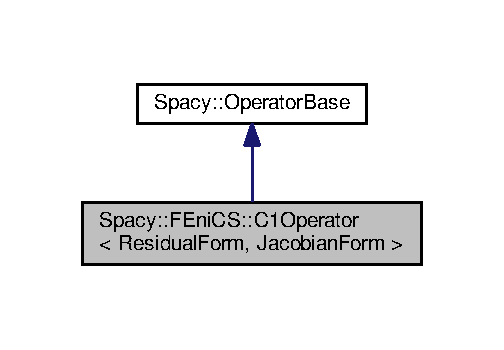
\includegraphics[width=243pt]{classSpacy_1_1FEniCS_1_1C1Operator__inherit__graph}
\end{center}
\end{figure}


Collaboration diagram for Spacy\+:\+:F\+Eni\+CS\+:\+:C1\+Operator$<$ Residual\+Form, Jacobian\+Form $>$\+:
\nopagebreak
\begin{figure}[H]
\begin{center}
\leavevmode
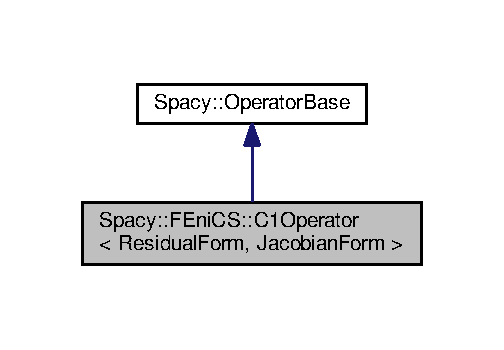
\includegraphics[width=243pt]{classSpacy_1_1FEniCS_1_1C1Operator__coll__graph}
\end{center}
\end{figure}
\subsection*{Public Member Functions}
\begin{DoxyCompactItemize}
\item 
\hyperlink{classSpacy_1_1FEniCS_1_1C1Operator_af23d84bd48d0902011bf80ba2f4cd394}{C1\+Operator} (const Residual\+Form \&F, const Jacobian\+Form \&J, const std\+::vector$<$ const dolfin\+::\+Dirichlet\+BC $\ast$ $>$ \&bcs, \hyperlink{classSpacy_1_1VectorSpace}{Vector\+Space} \&\hyperlink{classSpacy_1_1OperatorBase_a2588f9b3e0188820c4c494e63293dc6f}{domain}, \hyperlink{classSpacy_1_1VectorSpace}{Vector\+Space} \&\hyperlink{classSpacy_1_1OperatorBase_ab19d3b7a6f290b1079248f1e567e53d6}{range})
\begin{DoxyCompactList}\small\item\em Construct operator for F\+Enics. \end{DoxyCompactList}\item 
\hyperlink{classSpacy_1_1FEniCS_1_1C1Operator_afe6c4eb8960290212a16a1eca2267b48}{C1\+Operator} (const Residual\+Form \&F, const Jacobian\+Form \&J, \hyperlink{classSpacy_1_1VectorSpace}{Vector\+Space} \&\hyperlink{classSpacy_1_1OperatorBase_a2588f9b3e0188820c4c494e63293dc6f}{domain}, \hyperlink{classSpacy_1_1VectorSpace}{Vector\+Space} \&\hyperlink{classSpacy_1_1OperatorBase_ab19d3b7a6f290b1079248f1e567e53d6}{range})
\begin{DoxyCompactList}\small\item\em Construct operator without boundary conditions for F\+Enics. \end{DoxyCompactList}\item 
{\bfseries C1\+Operator} (\hyperlink{classSpacy_1_1FEniCS_1_1C1Operator}{C1\+Operator} \&\&other)\hypertarget{classSpacy_1_1FEniCS_1_1C1Operator_a4ab2b79f50f05b4cc4403269dad87e1e}{}\label{classSpacy_1_1FEniCS_1_1C1Operator_a4ab2b79f50f05b4cc4403269dad87e1e}

\item 
{\bfseries C1\+Operator} (const \hyperlink{classSpacy_1_1FEniCS_1_1C1Operator}{C1\+Operator} \&other)\hypertarget{classSpacy_1_1FEniCS_1_1C1Operator_a8bedc9295f43ebe21be9e2a9337da1e5}{}\label{classSpacy_1_1FEniCS_1_1C1Operator_a8bedc9295f43ebe21be9e2a9337da1e5}

\item 
\hyperlink{classSpacy_1_1FEniCS_1_1C1Operator}{C1\+Operator} \& {\bfseries operator=} (const \hyperlink{classSpacy_1_1FEniCS_1_1C1Operator}{C1\+Operator} \&other)\hypertarget{classSpacy_1_1FEniCS_1_1C1Operator_a1e74d332b9cb30ed83d757a39453c47c}{}\label{classSpacy_1_1FEniCS_1_1C1Operator_a1e74d332b9cb30ed83d757a39453c47c}

\item 
\hyperlink{classSpacy_1_1FEniCS_1_1C1Operator}{C1\+Operator} \& {\bfseries operator=} (\hyperlink{classSpacy_1_1FEniCS_1_1C1Operator}{C1\+Operator} \&\&other)\hypertarget{classSpacy_1_1FEniCS_1_1C1Operator_ae611721c1f172413877c91a3e99ae69b}{}\label{classSpacy_1_1FEniCS_1_1C1Operator_ae611721c1f172413877c91a3e99ae69b}

\item 
\+::\hyperlink{classSpacy_1_1Vector}{Spacy\+::\+Vector} \hyperlink{classSpacy_1_1FEniCS_1_1C1Operator_a5e2b3831a7583793f6c134eedd2be9bc}{operator()} (const \+::\hyperlink{classSpacy_1_1Vector}{Spacy\+::\+Vector} \&x) const \hypertarget{classSpacy_1_1FEniCS_1_1C1Operator_a5e2b3831a7583793f6c134eedd2be9bc}{}\label{classSpacy_1_1FEniCS_1_1C1Operator_a5e2b3831a7583793f6c134eedd2be9bc}

\begin{DoxyCompactList}\small\item\em Compute $A(x)$. \end{DoxyCompactList}\item 
\+::\hyperlink{classSpacy_1_1Vector}{Spacy\+::\+Vector} \hyperlink{classSpacy_1_1FEniCS_1_1C1Operator_a610d7a4a5daec3b512ab3ccf46a7b9e9}{d1} (const \+::\hyperlink{classSpacy_1_1Vector}{Spacy\+::\+Vector} \&x, const \+::\hyperlink{classSpacy_1_1Vector}{Spacy\+::\+Vector} \&dx) const \hypertarget{classSpacy_1_1FEniCS_1_1C1Operator_a610d7a4a5daec3b512ab3ccf46a7b9e9}{}\label{classSpacy_1_1FEniCS_1_1C1Operator_a610d7a4a5daec3b512ab3ccf46a7b9e9}

\begin{DoxyCompactList}\small\item\em Compute $A'(x)dx$. \end{DoxyCompactList}\item 
auto \hyperlink{classSpacy_1_1FEniCS_1_1C1Operator_aab603c2b35f2b710b2e646cf3fb7ee9c}{linearization} (const \+::\hyperlink{classSpacy_1_1Vector}{Spacy\+::\+Vector} \&x) const 
\begin{DoxyCompactList}\small\item\em Access $A'(x)$ as linear operator $X\rightarrow Y$. \end{DoxyCompactList}\item 
const \hyperlink{classSpacy_1_1VectorSpace}{Vector\+Space} \& \hyperlink{classSpacy_1_1OperatorBase_a2588f9b3e0188820c4c494e63293dc6f}{domain} () const \hypertarget{classSpacy_1_1OperatorBase_a2588f9b3e0188820c4c494e63293dc6f}{}\label{classSpacy_1_1OperatorBase_a2588f9b3e0188820c4c494e63293dc6f}

\begin{DoxyCompactList}\small\item\em Access domain space $X$. \end{DoxyCompactList}\item 
const \hyperlink{classSpacy_1_1VectorSpace}{Vector\+Space} \& \hyperlink{classSpacy_1_1OperatorBase_ab19d3b7a6f290b1079248f1e567e53d6}{range} () const \hypertarget{classSpacy_1_1OperatorBase_ab19d3b7a6f290b1079248f1e567e53d6}{}\label{classSpacy_1_1OperatorBase_ab19d3b7a6f290b1079248f1e567e53d6}

\begin{DoxyCompactList}\small\item\em Access range space $Y$. \end{DoxyCompactList}\end{DoxyCompactItemize}


\subsection{Detailed Description}
\subsubsection*{template$<$class Residual\+Form, class Jacobian\+Form$>$\\*
class Spacy\+::\+F\+Eni\+C\+S\+::\+C1\+Operator$<$ Residual\+Form, Jacobian\+Form $>$}

Operator interface for F\+Eni\+CS. Models a differentiable operator $A:X\rightarrow Y$. 

\begin{DoxyWarning}{Warning}
In the .ufl file you have to name the argument of $f$ by \char`\"{}x\char`\"{}! 
\end{DoxyWarning}
\begin{DoxySeeAlso}{See also}
C1\+Operator, C1\+Operator\+Concept 
\end{DoxySeeAlso}


\subsection{Constructor \& Destructor Documentation}
\index{Spacy\+::\+F\+Eni\+C\+S\+::\+C1\+Operator@{Spacy\+::\+F\+Eni\+C\+S\+::\+C1\+Operator}!C1\+Operator@{C1\+Operator}}
\index{C1\+Operator@{C1\+Operator}!Spacy\+::\+F\+Eni\+C\+S\+::\+C1\+Operator@{Spacy\+::\+F\+Eni\+C\+S\+::\+C1\+Operator}}
\subsubsection[{\texorpdfstring{C1\+Operator(const Residual\+Form \&\+F, const Jacobian\+Form \&\+J, const std\+::vector$<$ const dolfin\+::\+Dirichlet\+B\+C $\ast$ $>$ \&bcs, Vector\+Space \&domain, Vector\+Space \&range)}{C1Operator(const ResidualForm &F, const JacobianForm &J, const std::vector< const dolfin::DirichletBC * > &bcs, VectorSpace &domain, VectorSpace &range)}}]{\setlength{\rightskip}{0pt plus 5cm}template$<$class Residual\+Form , class Jacobian\+Form $>$ {\bf Spacy\+::\+F\+Eni\+C\+S\+::\+C1\+Operator}$<$ Residual\+Form, Jacobian\+Form $>$\+::{\bf C1\+Operator} (
\begin{DoxyParamCaption}
\item[{const Residual\+Form \&}]{F, }
\item[{const Jacobian\+Form \&}]{J, }
\item[{const std\+::vector$<$ const dolfin\+::\+Dirichlet\+BC $\ast$ $>$ \&}]{bcs, }
\item[{{\bf Vector\+Space} \&}]{domain, }
\item[{{\bf Vector\+Space} \&}]{range}
\end{DoxyParamCaption}
)\hspace{0.3cm}{\ttfamily [inline]}}\hypertarget{classSpacy_1_1FEniCS_1_1C1Operator_af23d84bd48d0902011bf80ba2f4cd394}{}\label{classSpacy_1_1FEniCS_1_1C1Operator_af23d84bd48d0902011bf80ba2f4cd394}


Construct operator for F\+Enics. 


\begin{DoxyParams}{Parameters}
{\em F} & Residual form for the evaluation of $A$ \\
\hline
{\em J} & Jacobian form for the evaluation of $A'$ \\
\hline
{\em bcs} & Dirichlet boundary conditions \\
\hline
{\em domain} & domain space $X$ \\
\hline
{\em range} & range space $Y$ \\
\hline
\end{DoxyParams}
\index{Spacy\+::\+F\+Eni\+C\+S\+::\+C1\+Operator@{Spacy\+::\+F\+Eni\+C\+S\+::\+C1\+Operator}!C1\+Operator@{C1\+Operator}}
\index{C1\+Operator@{C1\+Operator}!Spacy\+::\+F\+Eni\+C\+S\+::\+C1\+Operator@{Spacy\+::\+F\+Eni\+C\+S\+::\+C1\+Operator}}
\subsubsection[{\texorpdfstring{C1\+Operator(const Residual\+Form \&\+F, const Jacobian\+Form \&\+J, Vector\+Space \&domain, Vector\+Space \&range)}{C1Operator(const ResidualForm &F, const JacobianForm &J, VectorSpace &domain, VectorSpace &range)}}]{\setlength{\rightskip}{0pt plus 5cm}template$<$class Residual\+Form , class Jacobian\+Form $>$ {\bf Spacy\+::\+F\+Eni\+C\+S\+::\+C1\+Operator}$<$ Residual\+Form, Jacobian\+Form $>$\+::{\bf C1\+Operator} (
\begin{DoxyParamCaption}
\item[{const Residual\+Form \&}]{F, }
\item[{const Jacobian\+Form \&}]{J, }
\item[{{\bf Vector\+Space} \&}]{domain, }
\item[{{\bf Vector\+Space} \&}]{range}
\end{DoxyParamCaption}
)\hspace{0.3cm}{\ttfamily [inline]}}\hypertarget{classSpacy_1_1FEniCS_1_1C1Operator_afe6c4eb8960290212a16a1eca2267b48}{}\label{classSpacy_1_1FEniCS_1_1C1Operator_afe6c4eb8960290212a16a1eca2267b48}


Construct operator without boundary conditions for F\+Enics. 


\begin{DoxyParams}{Parameters}
{\em F} & Residual form for the evaluation of $A$ \\
\hline
{\em J} & Jacobian form for the evaluation of $A'$ \\
\hline
{\em domain} & domain space $X$ \\
\hline
{\em range} & range space $Y$ \\
\hline
\end{DoxyParams}


\subsection{Member Function Documentation}
\index{Spacy\+::\+F\+Eni\+C\+S\+::\+C1\+Operator@{Spacy\+::\+F\+Eni\+C\+S\+::\+C1\+Operator}!linearization@{linearization}}
\index{linearization@{linearization}!Spacy\+::\+F\+Eni\+C\+S\+::\+C1\+Operator@{Spacy\+::\+F\+Eni\+C\+S\+::\+C1\+Operator}}
\subsubsection[{\texorpdfstring{linearization(const \+::\+Spacy\+::\+Vector \&x) const }{linearization(const ::Spacy::Vector &x) const }}]{\setlength{\rightskip}{0pt plus 5cm}template$<$class Residual\+Form , class Jacobian\+Form $>$ auto {\bf Spacy\+::\+F\+Eni\+C\+S\+::\+C1\+Operator}$<$ Residual\+Form, Jacobian\+Form $>$\+::linearization (
\begin{DoxyParamCaption}
\item[{const \+::{\bf Spacy\+::\+Vector} \&}]{x}
\end{DoxyParamCaption}
) const\hspace{0.3cm}{\ttfamily [inline]}}\hypertarget{classSpacy_1_1FEniCS_1_1C1Operator_aab603c2b35f2b710b2e646cf3fb7ee9c}{}\label{classSpacy_1_1FEniCS_1_1C1Operator_aab603c2b35f2b710b2e646cf3fb7ee9c}


Access $A'(x)$ as linear operator $X\rightarrow Y$. 

\begin{DoxySeeAlso}{See also}
\hyperlink{classSpacy_1_1FEniCS_1_1LinearOperator}{Linear\+Operator}, \hyperlink{classSpacy_1_1LinearOperator}{Spacy\+::\+Linear\+Operator} 
\end{DoxySeeAlso}


The documentation for this class was generated from the following file\+:\begin{DoxyCompactItemize}
\item 
/home/lars/tmp/\+Spacy/\+Spacy/\+Adapter/\+F\+Eni\+C\+S/c1\+Operator.\+hh\end{DoxyCompactItemize}

\hypertarget{structSpacy_1_1C1OperatorDetail_1_1C1OperatorConcept}{\section{\-Spacy\-:\-:\-C1\-Operator\-Detail\-:\-:\-C1\-Operator\-Concept$<$ \-Impl, \-T, bool $>$ \-Struct \-Template \-Reference}
\label{structSpacy_1_1C1OperatorDetail_1_1C1OperatorConcept}\index{\-Spacy\-::\-C1\-Operator\-Detail\-::\-C1\-Operator\-Concept$<$ Impl, T, bool $>$@{\-Spacy\-::\-C1\-Operator\-Detail\-::\-C1\-Operator\-Concept$<$ Impl, T, bool $>$}}
}
\subsubsection*{template$<$class Impl, class T, bool = std\-::is\-\_\-same$<$ Impl, T $>$\-::value$>$ struct Spacy\-::\-C1\-Operator\-Detail\-::\-C1\-Operator\-Concept$<$ Impl, T, bool $>$}



\-The documentation for this struct was generated from the following file\-:\begin{DoxyCompactItemize}
\item 
/home/travis/build/spacy-\/dev/\-Spacy/\-Spacy/\-Detail/details\-\_\-for\-\_\-c1\-Operator.\-hh\end{DoxyCompactItemize}

\hypertarget{structSpacy_1_1C1OperatorDetail_1_1C1OperatorConcept_3_01Impl_00_01T_00_01false_01_4}{\section{\-Spacy\-:\-:\-C1\-Operator\-Detail\-:\-:\-C1\-Operator\-Concept$<$ \-Impl, \-T, false $>$ \-Struct \-Template \-Reference}
\label{structSpacy_1_1C1OperatorDetail_1_1C1OperatorConcept_3_01Impl_00_01T_00_01false_01_4}\index{\-Spacy\-::\-C1\-Operator\-Detail\-::\-C1\-Operator\-Concept$<$ Impl, T, false $>$@{\-Spacy\-::\-C1\-Operator\-Detail\-::\-C1\-Operator\-Concept$<$ Impl, T, false $>$}}
}


\-Inheritance diagram for \-Spacy\-:\-:\-C1\-Operator\-Detail\-:\-:\-C1\-Operator\-Concept$<$ \-Impl, \-T, false $>$\-:
\nopagebreak
\begin{figure}[H]
\begin{center}
\leavevmode
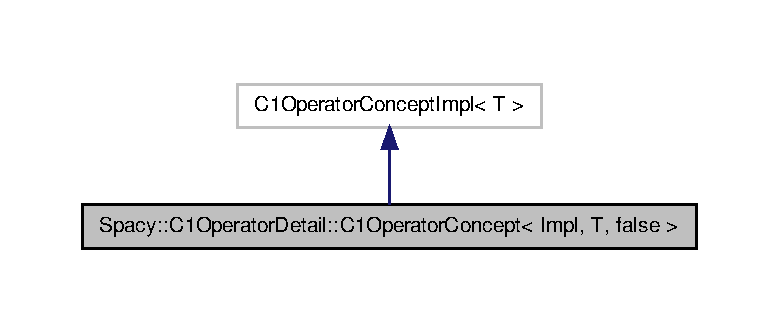
\includegraphics[width=350pt]{structSpacy_1_1C1OperatorDetail_1_1C1OperatorConcept_3_01Impl_00_01T_00_01false_01_4__inherit__graph}
\end{center}
\end{figure}


\-Collaboration diagram for \-Spacy\-:\-:\-C1\-Operator\-Detail\-:\-:\-C1\-Operator\-Concept$<$ \-Impl, \-T, false $>$\-:
\nopagebreak
\begin{figure}[H]
\begin{center}
\leavevmode
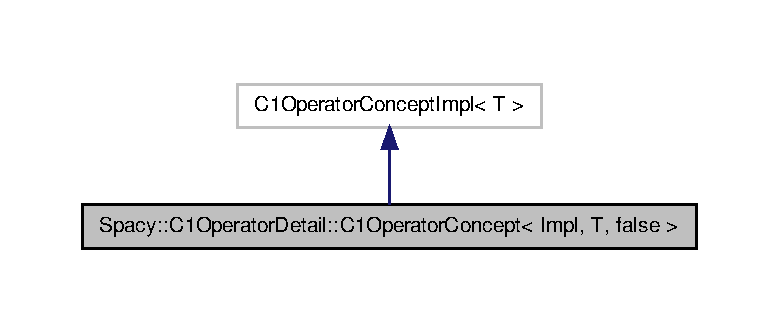
\includegraphics[width=350pt]{structSpacy_1_1C1OperatorDetail_1_1C1OperatorConcept_3_01Impl_00_01T_00_01false_01_4__coll__graph}
\end{center}
\end{figure}
\subsubsection*{template$<$class Impl, class T$>$ struct Spacy\-::\-C1\-Operator\-Detail\-::\-C1\-Operator\-Concept$<$ Impl, T, false $>$}



\-The documentation for this struct was generated from the following file\-:\begin{DoxyCompactItemize}
\item 
/home/travis/build/spacy-\/dev/\-Spacy/\-Spacy/\-Detail/details\-\_\-for\-\_\-c1\-Operator.\-hh\end{DoxyCompactItemize}

\hypertarget{classSpacy_1_1Kaskade_1_1C2Functional}{\section{Spacy\-:\-:Kaskade\-:\-:C2\-Functional$<$ Functional\-Definition $>$ Class Template Reference}
\label{classSpacy_1_1Kaskade_1_1C2Functional}\index{Spacy\-::\-Kaskade\-::\-C2\-Functional$<$ Functional\-Definition $>$@{Spacy\-::\-Kaskade\-::\-C2\-Functional$<$ Functional\-Definition $>$}}
}


Functional interface for Kaskade 7. Models a twice differentiable functional $f:X\rightarrow \mathbb{R}$.  




{\ttfamily \#include $<$c2\-Functional.\-hh$>$}



Inheritance diagram for Spacy\-:\-:Kaskade\-:\-:C2\-Functional$<$ Functional\-Definition $>$\-:
\nopagebreak
\begin{figure}[H]
\begin{center}
\leavevmode
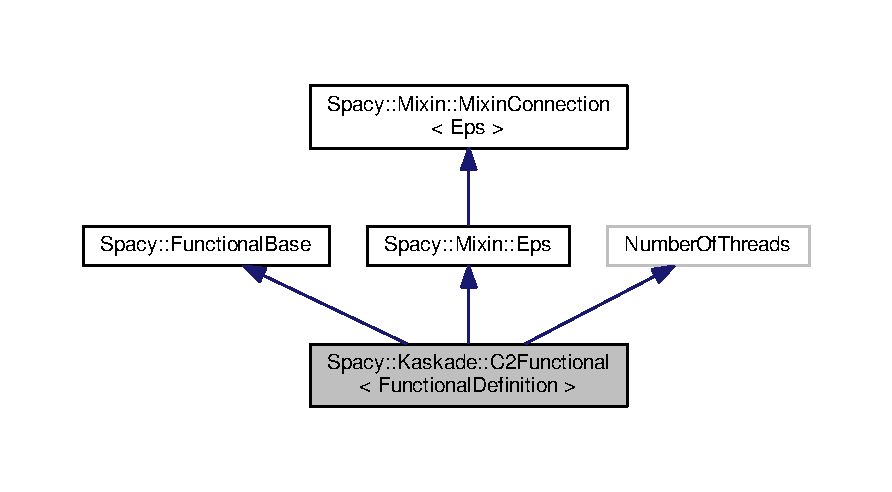
\includegraphics[width=350pt]{classSpacy_1_1Kaskade_1_1C2Functional__inherit__graph}
\end{center}
\end{figure}


Collaboration diagram for Spacy\-:\-:Kaskade\-:\-:C2\-Functional$<$ Functional\-Definition $>$\-:
\nopagebreak
\begin{figure}[H]
\begin{center}
\leavevmode
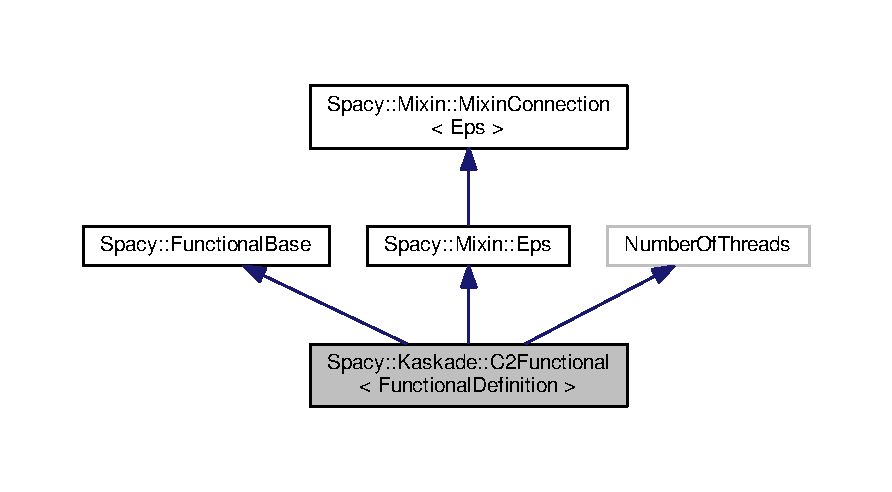
\includegraphics[width=350pt]{classSpacy_1_1Kaskade_1_1C2Functional__coll__graph}
\end{center}
\end{figure}
\subsection*{Public Types}
\begin{DoxyCompactItemize}
\item 
\hypertarget{classSpacy_1_1Kaskade_1_1C2Functional_a7f55d083d721b515160ce43336520e4e}{using \hyperlink{classSpacy_1_1Kaskade_1_1C2Functional_a7f55d083d721b515160ce43336520e4e}{Variable\-Set\-Description} = typename Functional\-Definition\-::\-Ansatz\-Vars}\label{classSpacy_1_1Kaskade_1_1C2Functional_a7f55d083d721b515160ce43336520e4e}

\begin{DoxyCompactList}\small\item\em Kaskade\-::\-Variable\-Set\-Description \end{DoxyCompactList}\item 
\hypertarget{classSpacy_1_1Kaskade_1_1C2Functional_a7845e44764fb2913ebc32153d6d90edf}{using \hyperlink{classSpacy_1_1Kaskade_1_1C2Functional_a7845e44764fb2913ebc32153d6d90edf}{Coefficient\-Vector} = typename Variable\-Set\-Description\-::template Coefficient\-Vector\-Representation$<$$>$\-::type}\label{classSpacy_1_1Kaskade_1_1C2Functional_a7845e44764fb2913ebc32153d6d90edf}

\begin{DoxyCompactList}\small\item\em Coefficient vector type. \end{DoxyCompactList}\item 
\hypertarget{classSpacy_1_1Kaskade_1_1C2Functional_afb866208161b4421f74aab07f50af065}{using \hyperlink{classSpacy_1_1Kaskade_1_1C2Functional_afb866208161b4421f74aab07f50af065}{Spaces} = typename Variable\-Set\-Description\-::\-Spaces}\label{classSpacy_1_1Kaskade_1_1C2Functional_afb866208161b4421f74aab07f50af065}

\begin{DoxyCompactList}\small\item\em boost\-::fusion\-::vector$<$const Space0$\ast$,const Space1$\ast$,...$>$ \end{DoxyCompactList}\item 
\hypertarget{classSpacy_1_1Kaskade_1_1C2Functional_ac4a1a2e519af22616ae7d6214c95b1ed}{using \hyperlink{classSpacy_1_1Kaskade_1_1C2Functional_ac4a1a2e519af22616ae7d6214c95b1ed}{Assembler} = \-::Kaskade\-::\-Variational\-Functional\-Assembler$<$ \-::Kaskade\-::\-Linearization\-At$<$ Functional\-Definition $>$ $>$}\label{classSpacy_1_1Kaskade_1_1C2Functional_ac4a1a2e519af22616ae7d6214c95b1ed}

\begin{DoxyCompactList}\small\item\em Kaskade\-::\-Variational\-Functional\-Assembler \end{DoxyCompactList}\item 
\hypertarget{classSpacy_1_1Kaskade_1_1C2Functional_aa7247706c3561818b2bf7d84c8841fe5}{using \hyperlink{classSpacy_1_1Kaskade_1_1C2Functional_aa7247706c3561818b2bf7d84c8841fe5}{Matrix} = \-::Kaskade\-::\-Matrix\-As\-Triplet$<$ double $>$}\label{classSpacy_1_1Kaskade_1_1C2Functional_aa7247706c3561818b2bf7d84c8841fe5}

\begin{DoxyCompactList}\small\item\em Matrix type. \end{DoxyCompactList}\item 
\hypertarget{classSpacy_1_1Kaskade_1_1C2Functional_af530f936729e854d2fd1401526149ba1}{using \hyperlink{classSpacy_1_1Kaskade_1_1C2Functional_af530f936729e854d2fd1401526149ba1}{Kaskade\-Operator} = \-::Kaskade\-::\-Matrix\-Represented\-Operator$<$ \hyperlink{classSpacy_1_1Kaskade_1_1C2Functional_aa7247706c3561818b2bf7d84c8841fe5}{Matrix}, \hyperlink{classSpacy_1_1Kaskade_1_1C2Functional_a7845e44764fb2913ebc32153d6d90edf}{Coefficient\-Vector}, \hyperlink{classSpacy_1_1Kaskade_1_1C2Functional_a7845e44764fb2913ebc32153d6d90edf}{Coefficient\-Vector} $>$}\label{classSpacy_1_1Kaskade_1_1C2Functional_af530f936729e854d2fd1401526149ba1}

\begin{DoxyCompactList}\small\item\em operator for the description of the second derivative \end{DoxyCompactList}\item 
\hypertarget{classSpacy_1_1Kaskade_1_1C2Functional_a2be6cba631e0718d78b731695f349814}{using {\bfseries Linearization} = \hyperlink{classSpacy_1_1Kaskade_1_1LinearOperator}{Linear\-Operator}$<$ \hyperlink{classSpacy_1_1Kaskade_1_1C2Functional_a7f55d083d721b515160ce43336520e4e}{Variable\-Set\-Description}, \hyperlink{classSpacy_1_1Kaskade_1_1C2Functional_a7f55d083d721b515160ce43336520e4e}{Variable\-Set\-Description} $>$}\label{classSpacy_1_1Kaskade_1_1C2Functional_a2be6cba631e0718d78b731695f349814}

\end{DoxyCompactItemize}
\subsection*{Public Member Functions}
\begin{DoxyCompactItemize}
\item 
\hyperlink{classSpacy_1_1Kaskade_1_1C2Functional_a35511ed1de0b2599efa901f27793dbdc}{C2\-Functional} (const Functional\-Definition \&f, const \hyperlink{classSpacy_1_1VectorSpace}{Vector\-Space} \&\hyperlink{classSpacy_1_1FunctionalBase_a2d3397deb9fa1ad85ed04e37a03b3aa6}{domain}, int rbegin=0, int rend=Functional\-Definition\-::\-Ansatz\-Vars\-::no\-Of\-Variables, int cbegin=0, int cend=Functional\-Definition\-::\-Test\-Vars\-::no\-Of\-Variables)
\begin{DoxyCompactList}\small\item\em Construct a twice differentiable functional $f: X\rightarrow \mathbb{R}$ from Kaskade 7. \end{DoxyCompactList}\item 
\hypertarget{classSpacy_1_1Kaskade_1_1C2Functional_ac74a454a44bdb24c484ac21e5f510dcf}{{\bfseries Number\-Of\-Threads} (g)}\label{classSpacy_1_1Kaskade_1_1C2Functional_ac74a454a44bdb24c484ac21e5f510dcf}

\item 
\hypertarget{classSpacy_1_1Kaskade_1_1C2Functional_a5ba70db6e6ca12902f095b0d5de48749}{{\bfseries f\-\_\-} (g.\-f\-\_\-)}\label{classSpacy_1_1Kaskade_1_1C2Functional_a5ba70db6e6ca12902f095b0d5de48749}

\item 
\hypertarget{classSpacy_1_1Kaskade_1_1C2Functional_a3de900f8fac6e4e91be19d254586a1f6}{{\bfseries spaces\-\_\-} (g.\-spaces\-\_\-)}\label{classSpacy_1_1Kaskade_1_1C2Functional_a3de900f8fac6e4e91be19d254586a1f6}

\item 
\hypertarget{classSpacy_1_1Kaskade_1_1C2Functional_ae7ad8ac9409c2f593510f8a54c49783c}{{\bfseries A\-\_\-} (g.\-A\-\_\-)}\label{classSpacy_1_1Kaskade_1_1C2Functional_ae7ad8ac9409c2f593510f8a54c49783c}

\item 
\hypertarget{classSpacy_1_1Kaskade_1_1C2Functional_a49f95c673c4e7de34bf1c6c0198f6103}{{\bfseries value\-\_\-} (g.\-value\-\_\-)}\label{classSpacy_1_1Kaskade_1_1C2Functional_a49f95c673c4e7de34bf1c6c0198f6103}

\item 
\hypertarget{classSpacy_1_1Kaskade_1_1C2Functional_a234297689b87c5d511da1fb7d57b2980}{{\bfseries old\-\_\-\-X\-\_\-f\-\_\-} (g.\-old\-\_\-\-X\-\_\-f\-\_\-)}\label{classSpacy_1_1Kaskade_1_1C2Functional_a234297689b87c5d511da1fb7d57b2980}

\item 
\hypertarget{classSpacy_1_1Kaskade_1_1C2Functional_af77b8c12b3adcab92f4629349ca45754}{{\bfseries old\-\_\-\-X\-\_\-df\-\_\-} (g.\-old\-\_\-\-X\-\_\-df\-\_\-)}\label{classSpacy_1_1Kaskade_1_1C2Functional_af77b8c12b3adcab92f4629349ca45754}

\item 
\hypertarget{classSpacy_1_1Kaskade_1_1C2Functional_a1bde54a791cc90f50c414b74c24ce378}{{\bfseries old\-\_\-\-X\-\_\-ddf\-\_\-} (g.\-old\-\_\-\-X\-\_\-ddf\-\_\-)}\label{classSpacy_1_1Kaskade_1_1C2Functional_a1bde54a791cc90f50c414b74c24ce378}

\item 
\hypertarget{classSpacy_1_1Kaskade_1_1C2Functional_ae86552c5bf14325af3d5dad1519328c1}{{\bfseries rhs\-\_\-} (g.\-rhs\-\_\-)}\label{classSpacy_1_1Kaskade_1_1C2Functional_ae86552c5bf14325af3d5dad1519328c1}

\item 
\hypertarget{classSpacy_1_1Kaskade_1_1C2Functional_a19cfc6ed02c41f488e60ba92d5443963}{{\bfseries only\-Lower\-Triangle\-\_\-} (g.\-only\-Lower\-Triangle\-\_\-)}\label{classSpacy_1_1Kaskade_1_1C2Functional_a19cfc6ed02c41f488e60ba92d5443963}

\item 
\hypertarget{classSpacy_1_1Kaskade_1_1C2Functional_a6218efc79570a1965cb0e6c16849bea7}{{\bfseries rbegin\-\_\-} (g.\-rbegin\-\_\-)}\label{classSpacy_1_1Kaskade_1_1C2Functional_a6218efc79570a1965cb0e6c16849bea7}

\item 
\hypertarget{classSpacy_1_1Kaskade_1_1C2Functional_abf8d7a7600914b718b6d640b6d146578}{{\bfseries rend\-\_\-} (g.\-rend\-\_\-)}\label{classSpacy_1_1Kaskade_1_1C2Functional_abf8d7a7600914b718b6d640b6d146578}

\item 
\hypertarget{classSpacy_1_1Kaskade_1_1C2Functional_a815238535fee49facc2254d5217c37b3}{{\bfseries cbegin\-\_\-} (g.\-cbegin\-\_\-)}\label{classSpacy_1_1Kaskade_1_1C2Functional_a815238535fee49facc2254d5217c37b3}

\item 
\hypertarget{classSpacy_1_1Kaskade_1_1C2Functional_a5dec607a12b95d984ceeb1bf7f0b9383}{{\bfseries cend\-\_\-} (g.\-cend\-\_\-)}\label{classSpacy_1_1Kaskade_1_1C2Functional_a5dec607a12b95d984ceeb1bf7f0b9383}

\item 
\hypertarget{classSpacy_1_1Kaskade_1_1C2Functional_a179dfe5d74942f7bb7ce7112eec001fe}{{\bfseries solver\-Creator\-\_\-} (g.\-solver\-Creator\-\_\-)}\label{classSpacy_1_1Kaskade_1_1C2Functional_a179dfe5d74942f7bb7ce7112eec001fe}

\item 
\hypertarget{classSpacy_1_1Kaskade_1_1C2Functional_a96a7f6a98f4f7e20c543792fc9d00626}{{\bfseries operator\-Space\-\_\-} (g.\-operator\-Space\-\_\-)}\label{classSpacy_1_1Kaskade_1_1C2Functional_a96a7f6a98f4f7e20c543792fc9d00626}

\item 
\hyperlink{classSpacy_1_1Kaskade_1_1C2Functional}{C2\-Functional} \& \hyperlink{classSpacy_1_1Kaskade_1_1C2Functional_a1e24c0959890ba4caf0531cf47f3bee5}{operator=} (const \hyperlink{classSpacy_1_1Kaskade_1_1C2Functional}{C2\-Functional} \&g)
\begin{DoxyCompactList}\small\item\em Copy assignment. \end{DoxyCompactList}\item 
\hyperlink{classSpacy_1_1Kaskade_1_1C2Functional_adf3cb62771e39a351db349005ec6bc36}{C2\-Functional} (\hyperlink{classSpacy_1_1Kaskade_1_1C2Functional}{C2\-Functional} \&\&g)=default
\begin{DoxyCompactList}\small\item\em Move constructor. \end{DoxyCompactList}\item 
\hyperlink{classSpacy_1_1Kaskade_1_1C2Functional}{C2\-Functional} \& \hyperlink{classSpacy_1_1Kaskade_1_1C2Functional_a2cabb743e80fa24c22ef0ac358159323}{operator=} (\hyperlink{classSpacy_1_1Kaskade_1_1C2Functional}{C2\-Functional} \&\&g)=default
\begin{DoxyCompactList}\small\item\em Move assignment. \end{DoxyCompactList}\item 
\hyperlink{classSpacy_1_1Real}{Real} \hyperlink{classSpacy_1_1Kaskade_1_1C2Functional_a74b955be1cc2cb7de4e66b434428fd89}{operator()} (const \-::\hyperlink{classSpacy_1_1Vector}{Spacy\-::\-Vector} \&x) const 
\begin{DoxyCompactList}\small\item\em Apply functional. \end{DoxyCompactList}\item 
\-::\hyperlink{classSpacy_1_1Vector}{Spacy\-::\-Vector} \hyperlink{classSpacy_1_1Kaskade_1_1C2Functional_a69d3260b5313bd495e8f5871b15738db}{d1} (const \-::\hyperlink{classSpacy_1_1Vector}{Spacy\-::\-Vector} \&x) const 
\begin{DoxyCompactList}\small\item\em Compute first directional derivative $f'(x) \in X^* $. \end{DoxyCompactList}\item 
\-::\hyperlink{classSpacy_1_1Vector}{Spacy\-::\-Vector} \hyperlink{classSpacy_1_1Kaskade_1_1C2Functional_a7bd6c110c1f954a92f43f6035787a9f0}{d2} (const \-::\hyperlink{classSpacy_1_1Vector}{Spacy\-::\-Vector} \&x, const \-::\hyperlink{classSpacy_1_1Vector}{Spacy\-::\-Vector} \&dx) const 
\begin{DoxyCompactList}\small\item\em Compute second directional derivative $f''(x)dx\in X^* $. \end{DoxyCompactList}\item 
auto \hyperlink{classSpacy_1_1Kaskade_1_1C2Functional_a73e0b9a2499e89bf85eddf1aa74fe9ba}{hessian} (const \-::\hyperlink{classSpacy_1_1Vector}{Spacy\-::\-Vector} \&x) const 
\begin{DoxyCompactList}\small\item\em Access $f''(x)$ as linear operator $X\rightarrow X^*$. \end{DoxyCompactList}\item 
\hypertarget{classSpacy_1_1Kaskade_1_1C2Functional_ab45aa1c81e4698b642a5381a9b6be14b}{const \hyperlink{classSpacy_1_1Kaskade_1_1C2Functional_af530f936729e854d2fd1401526149ba1}{Kaskade\-Operator} \& \hyperlink{classSpacy_1_1Kaskade_1_1C2Functional_ab45aa1c81e4698b642a5381a9b6be14b}{A} () const noexcept}\label{classSpacy_1_1Kaskade_1_1C2Functional_ab45aa1c81e4698b642a5381a9b6be14b}

\begin{DoxyCompactList}\small\item\em Access operator representing $f''$. \end{DoxyCompactList}\item 
\hypertarget{classSpacy_1_1Kaskade_1_1C2Functional_ac334455723ea59d001fef33e056b1ea7}{const \hyperlink{classSpacy_1_1Kaskade_1_1C2Functional_afb866208161b4421f74aab07f50af065}{Spaces} \& \hyperlink{classSpacy_1_1Kaskade_1_1C2Functional_ac334455723ea59d001fef33e056b1ea7}{spaces} () const noexcept}\label{classSpacy_1_1Kaskade_1_1C2Functional_ac334455723ea59d001fef33e056b1ea7}

\begin{DoxyCompactList}\small\item\em Access boost\-::fusion\-::vector of pointers to spaces. \end{DoxyCompactList}\item 
bool \hyperlink{classSpacy_1_1Kaskade_1_1C2Functional_a37152b2b1413e611d229a61318b86768}{only\-Lower\-Triangle} () const noexcept
\begin{DoxyCompactList}\small\item\em Access only\-Lower\-Triangle flag. \end{DoxyCompactList}\item 
void \hyperlink{classSpacy_1_1Kaskade_1_1C2Functional_ac9496fdef4f38eb466d5b5b58089be8b}{set\-Solver\-Creator} (std\-::function$<$ \hyperlink{namespaceSpacy_adcd0d78166a9c972b8a2e5a689fc2d03}{Linear\-Solver}(const \hyperlink{classSpacy_1_1Kaskade_1_1LinearOperator}{Linearization} \&)$>$ f)
\begin{DoxyCompactList}\small\item\em Change solver creator. \end{DoxyCompactList}\item 
\hypertarget{classSpacy_1_1FunctionalBase_a2d3397deb9fa1ad85ed04e37a03b3aa6}{const \hyperlink{classSpacy_1_1VectorSpace}{Vector\-Space} \& \hyperlink{classSpacy_1_1FunctionalBase_a2d3397deb9fa1ad85ed04e37a03b3aa6}{domain} () const }\label{classSpacy_1_1FunctionalBase_a2d3397deb9fa1ad85ed04e37a03b3aa6}

\begin{DoxyCompactList}\small\item\em Access domain space $X$. \end{DoxyCompactList}\item 
\hypertarget{classSpacy_1_1Mixin_1_1Eps_a818ab6dfab5e4eea583e1302bcc621f8}{void {\bfseries set\-\_\-eps} (\hyperlink{classSpacy_1_1Real}{Real} \hyperlink{classSpacy_1_1Mixin_1_1Eps_a812b99b0abc1d78a34b4114907f23f52}{eps})}\label{classSpacy_1_1Mixin_1_1Eps_a818ab6dfab5e4eea583e1302bcc621f8}

\item 
\hypertarget{classSpacy_1_1Mixin_1_1Eps_a812b99b0abc1d78a34b4114907f23f52}{\hyperlink{classSpacy_1_1Real}{Real} \hyperlink{classSpacy_1_1Mixin_1_1Eps_a812b99b0abc1d78a34b4114907f23f52}{eps} () const noexcept}\label{classSpacy_1_1Mixin_1_1Eps_a812b99b0abc1d78a34b4114907f23f52}

\begin{DoxyCompactList}\small\item\em Access $\varepsilon$. \end{DoxyCompactList}\item 
\hypertarget{classSpacy_1_1Mixin_1_1Eps_a1c1b0ed7f14ed4967dc7da9295a136d4}{\hyperlink{classSpacy_1_1Real}{Real} \hyperlink{classSpacy_1_1Mixin_1_1Eps_a1c1b0ed7f14ed4967dc7da9295a136d4}{sqrt\-\_\-eps} () const noexcept}\label{classSpacy_1_1Mixin_1_1Eps_a1c1b0ed7f14ed4967dc7da9295a136d4}

\begin{DoxyCompactList}\small\item\em Access $\sqrt\varepsilon$. \end{DoxyCompactList}\item 
\hypertarget{classSpacy_1_1Mixin_1_1Eps_a91dbe45e297be2bc53f1a96107a58c64}{\hyperlink{classSpacy_1_1Real}{Real} \hyperlink{classSpacy_1_1Mixin_1_1Eps_a91dbe45e297be2bc53f1a96107a58c64}{cbrt\-\_\-eps} () const noexcept}\label{classSpacy_1_1Mixin_1_1Eps_a91dbe45e297be2bc53f1a96107a58c64}

\begin{DoxyCompactList}\small\item\em Access $\varepsilon^{1/3}$. \end{DoxyCompactList}\item 
\hypertarget{classSpacy_1_1Mixin_1_1Eps_a151216968daef3da5f5cdc0b957ce01b}{void \hyperlink{classSpacy_1_1Mixin_1_1Eps_a151216968daef3da5f5cdc0b957ce01b}{update} (\hyperlink{classSpacy_1_1Mixin_1_1Eps_af616ae8e55a645cefd4d2d4504d6705a}{Eps} $\ast$changed\-Subject)}\label{classSpacy_1_1Mixin_1_1Eps_a151216968daef3da5f5cdc0b957ce01b}

\begin{DoxyCompactList}\small\item\em update function for observer pattern. \end{DoxyCompactList}\item 
\hypertarget{classSpacy_1_1Mixin_1_1MixinConnection_abb5520ee6b22dd993d78f142939a1ed4}{void \hyperlink{classSpacy_1_1Mixin_1_1MixinConnection_abb5520ee6b22dd993d78f142939a1ed4}{attach} (\hyperlink{classSpacy_1_1Mixin_1_1Eps_af616ae8e55a645cefd4d2d4504d6705a}{Eps} \&observer)}\label{classSpacy_1_1Mixin_1_1MixinConnection_abb5520ee6b22dd993d78f142939a1ed4}

\begin{DoxyCompactList}\small\item\em Attach observer. \end{DoxyCompactList}\item 
\hypertarget{classSpacy_1_1Mixin_1_1MixinConnection_adda739590c487679c26f60e50aedb73f}{void \hyperlink{classSpacy_1_1Mixin_1_1MixinConnection_adda739590c487679c26f60e50aedb73f}{detach} (\hyperlink{classSpacy_1_1Mixin_1_1Eps_af616ae8e55a645cefd4d2d4504d6705a}{Eps} \&observer)}\label{classSpacy_1_1Mixin_1_1MixinConnection_adda739590c487679c26f60e50aedb73f}

\begin{DoxyCompactList}\small\item\em Detach observer. \end{DoxyCompactList}\item 
\hypertarget{classSpacy_1_1Mixin_1_1MixinConnection_a1ddeaa78a3bb4a38c2cca36d1f99fe36}{void \hyperlink{classSpacy_1_1Mixin_1_1MixinConnection_a1ddeaa78a3bb4a38c2cca36d1f99fe36}{notify} ()}\label{classSpacy_1_1Mixin_1_1MixinConnection_a1ddeaa78a3bb4a38c2cca36d1f99fe36}

\begin{DoxyCompactList}\small\item\em Notify observers about changes. \end{DoxyCompactList}\end{DoxyCompactItemize}
\subsection*{Public Attributes}
\begin{DoxyCompactItemize}
\item 
{\bfseries true}
\end{DoxyCompactItemize}


\subsection{Detailed Description}
\subsubsection*{template$<$class Functional\-Definition$>$class Spacy\-::\-Kaskade\-::\-C2\-Functional$<$ Functional\-Definition $>$}

Functional interface for Kaskade 7. Models a twice differentiable functional $f:X\rightarrow \mathbb{R}$. 


\begin{DoxyTemplParams}{Template Parameters}
{\em Functional\-Definition} & functional definition from Kaskade 7 \\
\hline
\end{DoxyTemplParams}
\begin{DoxySeeAlso}{See Also}
\hyperlink{classSpacy_1_1C2Functional}{Spacy\-::\-C2\-Functional} 
\end{DoxySeeAlso}


\subsection{Constructor \& Destructor Documentation}
\hypertarget{classSpacy_1_1Kaskade_1_1C2Functional_a35511ed1de0b2599efa901f27793dbdc}{\index{Spacy\-::\-Kaskade\-::\-C2\-Functional@{Spacy\-::\-Kaskade\-::\-C2\-Functional}!C2\-Functional@{C2\-Functional}}
\index{C2\-Functional@{C2\-Functional}!Spacy::Kaskade::C2Functional@{Spacy\-::\-Kaskade\-::\-C2\-Functional}}
\subsubsection[{C2\-Functional}]{\setlength{\rightskip}{0pt plus 5cm}template$<$class Functional\-Definition$>$ {\bf Spacy\-::\-Kaskade\-::\-C2\-Functional}$<$ Functional\-Definition $>$\-::{\bf C2\-Functional} (
\begin{DoxyParamCaption}
\item[{const Functional\-Definition \&}]{f, }
\item[{const {\bf Vector\-Space} \&}]{domain, }
\item[{int}]{rbegin = {\ttfamily 0}, }
\item[{int}]{rend = {\ttfamily FunctionalDefinition\-:\-:AnsatzVars\-:\-:noOfVariables}, }
\item[{int}]{cbegin = {\ttfamily 0}, }
\item[{int}]{cend = {\ttfamily FunctionalDefinition\-:\-:TestVars\-:\-:noOfVariables}}
\end{DoxyParamCaption}
)\hspace{0.3cm}{\ttfamily [inline]}}}\label{classSpacy_1_1Kaskade_1_1C2Functional_a35511ed1de0b2599efa901f27793dbdc}


Construct a twice differentiable functional $f: X\rightarrow \mathbb{R}$ from Kaskade 7. 


\begin{DoxyParams}{Parameters}
{\em f} & operator definition from Kaskade 7 \\
\hline
{\em domain} & domain space \\
\hline
{\em rbegin} & first row to be considered in the definition of f \\
\hline
{\em rend} & one after the last row to be considered in the definition of f \\
\hline
{\em cbegin} & first column to be considered in the definition of f \\
\hline
{\em cend} & one after the last column to be considered in the definition of f\\
\hline
\end{DoxyParams}
The optional parameters rbegin, rend, cbegin and cend can be used to define operators that correspond to parts of a system of equation. \hypertarget{classSpacy_1_1Kaskade_1_1C2Functional_adf3cb62771e39a351db349005ec6bc36}{\index{Spacy\-::\-Kaskade\-::\-C2\-Functional@{Spacy\-::\-Kaskade\-::\-C2\-Functional}!C2\-Functional@{C2\-Functional}}
\index{C2\-Functional@{C2\-Functional}!Spacy::Kaskade::C2Functional@{Spacy\-::\-Kaskade\-::\-C2\-Functional}}
\subsubsection[{C2\-Functional}]{\setlength{\rightskip}{0pt plus 5cm}template$<$class Functional\-Definition$>$ {\bf Spacy\-::\-Kaskade\-::\-C2\-Functional}$<$ Functional\-Definition $>$\-::{\bf C2\-Functional} (
\begin{DoxyParamCaption}
\item[{{\bf C2\-Functional}$<$ Functional\-Definition $>$ \&\&}]{g}
\end{DoxyParamCaption}
)\hspace{0.3cm}{\ttfamily [default]}}}\label{classSpacy_1_1Kaskade_1_1C2Functional_adf3cb62771e39a351db349005ec6bc36}


Move constructor. 


\begin{DoxyParams}{Parameters}
{\em g} & functional to move from \\
\hline
\end{DoxyParams}


\subsection{Member Function Documentation}
\hypertarget{classSpacy_1_1Kaskade_1_1C2Functional_a1e24c0959890ba4caf0531cf47f3bee5}{\index{Spacy\-::\-Kaskade\-::\-C2\-Functional@{Spacy\-::\-Kaskade\-::\-C2\-Functional}!operator=@{operator=}}
\index{operator=@{operator=}!Spacy::Kaskade::C2Functional@{Spacy\-::\-Kaskade\-::\-C2\-Functional}}
\subsubsection[{operator=}]{\setlength{\rightskip}{0pt plus 5cm}template$<$class Functional\-Definition$>$ {\bf C2\-Functional}\& {\bf Spacy\-::\-Kaskade\-::\-C2\-Functional}$<$ Functional\-Definition $>$\-::operator= (
\begin{DoxyParamCaption}
\item[{const {\bf C2\-Functional}$<$ Functional\-Definition $>$ \&}]{g}
\end{DoxyParamCaption}
)\hspace{0.3cm}{\ttfamily [inline]}}}\label{classSpacy_1_1Kaskade_1_1C2Functional_a1e24c0959890ba4caf0531cf47f3bee5}


Copy assignment. 


\begin{DoxyParams}{Parameters}
{\em g} & functional to copy from \\
\hline
\end{DoxyParams}
\hypertarget{classSpacy_1_1Kaskade_1_1C2Functional_a2cabb743e80fa24c22ef0ac358159323}{\index{Spacy\-::\-Kaskade\-::\-C2\-Functional@{Spacy\-::\-Kaskade\-::\-C2\-Functional}!operator=@{operator=}}
\index{operator=@{operator=}!Spacy::Kaskade::C2Functional@{Spacy\-::\-Kaskade\-::\-C2\-Functional}}
\subsubsection[{operator=}]{\setlength{\rightskip}{0pt plus 5cm}template$<$class Functional\-Definition$>$ {\bf C2\-Functional}\& {\bf Spacy\-::\-Kaskade\-::\-C2\-Functional}$<$ Functional\-Definition $>$\-::operator= (
\begin{DoxyParamCaption}
\item[{{\bf C2\-Functional}$<$ Functional\-Definition $>$ \&\&}]{g}
\end{DoxyParamCaption}
)\hspace{0.3cm}{\ttfamily [default]}}}\label{classSpacy_1_1Kaskade_1_1C2Functional_a2cabb743e80fa24c22ef0ac358159323}


Move assignment. 


\begin{DoxyParams}{Parameters}
{\em g} & functional to move from \\
\hline
\end{DoxyParams}
\hypertarget{classSpacy_1_1Kaskade_1_1C2Functional_a74b955be1cc2cb7de4e66b434428fd89}{\index{Spacy\-::\-Kaskade\-::\-C2\-Functional@{Spacy\-::\-Kaskade\-::\-C2\-Functional}!operator()@{operator()}}
\index{operator()@{operator()}!Spacy::Kaskade::C2Functional@{Spacy\-::\-Kaskade\-::\-C2\-Functional}}
\subsubsection[{operator()}]{\setlength{\rightskip}{0pt plus 5cm}template$<$class Functional\-Definition$>$ {\bf Real} {\bf Spacy\-::\-Kaskade\-::\-C2\-Functional}$<$ Functional\-Definition $>$\-::operator() (
\begin{DoxyParamCaption}
\item[{const \-::{\bf Spacy\-::\-Vector} \&}]{x}
\end{DoxyParamCaption}
) const\hspace{0.3cm}{\ttfamily [inline]}}}\label{classSpacy_1_1Kaskade_1_1C2Functional_a74b955be1cc2cb7de4e66b434428fd89}


Apply functional. 


\begin{DoxyParams}{Parameters}
{\em x} & argument \\
\hline
\end{DoxyParams}
\begin{DoxyReturn}{Returns}
$f(x)$ 
\end{DoxyReturn}
\hypertarget{classSpacy_1_1Kaskade_1_1C2Functional_a69d3260b5313bd495e8f5871b15738db}{\index{Spacy\-::\-Kaskade\-::\-C2\-Functional@{Spacy\-::\-Kaskade\-::\-C2\-Functional}!d1@{d1}}
\index{d1@{d1}!Spacy::Kaskade::C2Functional@{Spacy\-::\-Kaskade\-::\-C2\-Functional}}
\subsubsection[{d1}]{\setlength{\rightskip}{0pt plus 5cm}template$<$class Functional\-Definition$>$ \-::{\bf Spacy\-::\-Vector} {\bf Spacy\-::\-Kaskade\-::\-C2\-Functional}$<$ Functional\-Definition $>$\-::d1 (
\begin{DoxyParamCaption}
\item[{const \-::{\bf Spacy\-::\-Vector} \&}]{x}
\end{DoxyParamCaption}
) const\hspace{0.3cm}{\ttfamily [inline]}}}\label{classSpacy_1_1Kaskade_1_1C2Functional_a69d3260b5313bd495e8f5871b15738db}


Compute first directional derivative $f'(x) \in X^* $. 


\begin{DoxyParams}{Parameters}
{\em x} & current iterate \\
\hline
\end{DoxyParams}
\begin{DoxyReturn}{Returns}
$f'(x)$ 
\end{DoxyReturn}
\hypertarget{classSpacy_1_1Kaskade_1_1C2Functional_a7bd6c110c1f954a92f43f6035787a9f0}{\index{Spacy\-::\-Kaskade\-::\-C2\-Functional@{Spacy\-::\-Kaskade\-::\-C2\-Functional}!d2@{d2}}
\index{d2@{d2}!Spacy::Kaskade::C2Functional@{Spacy\-::\-Kaskade\-::\-C2\-Functional}}
\subsubsection[{d2}]{\setlength{\rightskip}{0pt plus 5cm}template$<$class Functional\-Definition$>$ \-::{\bf Spacy\-::\-Vector} {\bf Spacy\-::\-Kaskade\-::\-C2\-Functional}$<$ Functional\-Definition $>$\-::d2 (
\begin{DoxyParamCaption}
\item[{const \-::{\bf Spacy\-::\-Vector} \&}]{x, }
\item[{const \-::{\bf Spacy\-::\-Vector} \&}]{dx}
\end{DoxyParamCaption}
) const\hspace{0.3cm}{\ttfamily [inline]}}}\label{classSpacy_1_1Kaskade_1_1C2Functional_a7bd6c110c1f954a92f43f6035787a9f0}


Compute second directional derivative $f''(x)dx\in X^* $. 


\begin{DoxyParams}{Parameters}
{\em x} & current iterate \\
\hline
{\em dx} & perturbation \\
\hline
\end{DoxyParams}
\begin{DoxyReturn}{Returns}
$f''(x)dx$ 
\end{DoxyReturn}
\hypertarget{classSpacy_1_1Kaskade_1_1C2Functional_a73e0b9a2499e89bf85eddf1aa74fe9ba}{\index{Spacy\-::\-Kaskade\-::\-C2\-Functional@{Spacy\-::\-Kaskade\-::\-C2\-Functional}!hessian@{hessian}}
\index{hessian@{hessian}!Spacy::Kaskade::C2Functional@{Spacy\-::\-Kaskade\-::\-C2\-Functional}}
\subsubsection[{hessian}]{\setlength{\rightskip}{0pt plus 5cm}template$<$class Functional\-Definition$>$ auto {\bf Spacy\-::\-Kaskade\-::\-C2\-Functional}$<$ Functional\-Definition $>$\-::hessian (
\begin{DoxyParamCaption}
\item[{const \-::{\bf Spacy\-::\-Vector} \&}]{x}
\end{DoxyParamCaption}
) const\hspace{0.3cm}{\ttfamily [inline]}}}\label{classSpacy_1_1Kaskade_1_1C2Functional_a73e0b9a2499e89bf85eddf1aa74fe9ba}


Access $f''(x)$ as linear operator $X\rightarrow X^*$. 


\begin{DoxyParams}{Parameters}
{\em x} & point of linearization \\
\hline
\end{DoxyParams}
\begin{DoxySeeAlso}{See Also}
\hyperlink{classSpacy_1_1Kaskade_1_1LinearOperator}{Linear\-Operator}, \hyperlink{classSpacy_1_1LinearOperator}{Spacy\-::\-Linear\-Operator} 
\end{DoxySeeAlso}
\hypertarget{classSpacy_1_1Kaskade_1_1C2Functional_a37152b2b1413e611d229a61318b86768}{\index{Spacy\-::\-Kaskade\-::\-C2\-Functional@{Spacy\-::\-Kaskade\-::\-C2\-Functional}!only\-Lower\-Triangle@{only\-Lower\-Triangle}}
\index{only\-Lower\-Triangle@{only\-Lower\-Triangle}!Spacy::Kaskade::C2Functional@{Spacy\-::\-Kaskade\-::\-C2\-Functional}}
\subsubsection[{only\-Lower\-Triangle}]{\setlength{\rightskip}{0pt plus 5cm}template$<$class Functional\-Definition$>$ bool {\bf Spacy\-::\-Kaskade\-::\-C2\-Functional}$<$ Functional\-Definition $>$\-::only\-Lower\-Triangle (
\begin{DoxyParamCaption}
{}
\end{DoxyParamCaption}
) const\hspace{0.3cm}{\ttfamily [inline]}, {\ttfamily [noexcept]}}}\label{classSpacy_1_1Kaskade_1_1C2Functional_a37152b2b1413e611d229a61318b86768}


Access only\-Lower\-Triangle flag. 

\begin{DoxyReturn}{Returns}
true if only the lower triangle of a symmetric matrix is stored in the operator definition, else false 
\end{DoxyReturn}
\hypertarget{classSpacy_1_1Kaskade_1_1C2Functional_ac9496fdef4f38eb466d5b5b58089be8b}{\index{Spacy\-::\-Kaskade\-::\-C2\-Functional@{Spacy\-::\-Kaskade\-::\-C2\-Functional}!set\-Solver\-Creator@{set\-Solver\-Creator}}
\index{set\-Solver\-Creator@{set\-Solver\-Creator}!Spacy::Kaskade::C2Functional@{Spacy\-::\-Kaskade\-::\-C2\-Functional}}
\subsubsection[{set\-Solver\-Creator}]{\setlength{\rightskip}{0pt plus 5cm}template$<$class Functional\-Definition$>$ void {\bf Spacy\-::\-Kaskade\-::\-C2\-Functional}$<$ Functional\-Definition $>$\-::set\-Solver\-Creator (
\begin{DoxyParamCaption}
\item[{std\-::function$<$ {\bf Linear\-Solver}(const {\bf Linearization} \&)$>$}]{f}
\end{DoxyParamCaption}
)\hspace{0.3cm}{\ttfamily [inline]}}}\label{classSpacy_1_1Kaskade_1_1C2Functional_ac9496fdef4f38eb466d5b5b58089be8b}


Change solver creator. 


\begin{DoxyParams}{Parameters}
{\em f} & function/functor for the creation of a linear solver \\
\hline
\end{DoxyParams}


\subsection{Member Data Documentation}
\hypertarget{classSpacy_1_1Kaskade_1_1C2Functional_a4f225221bbaf1f2e9707b7c11d5ba16d}{\index{Spacy\-::\-Kaskade\-::\-C2\-Functional@{Spacy\-::\-Kaskade\-::\-C2\-Functional}!true@{true}}
\index{true@{true}!Spacy::Kaskade::C2Functional@{Spacy\-::\-Kaskade\-::\-C2\-Functional}}
\subsubsection[{true}]{\setlength{\rightskip}{0pt plus 5cm}template$<$class Functional\-Definition$>$ {\bf Spacy\-::\-Kaskade\-::\-C2\-Functional}$<$ Functional\-Definition $>$\-::true}}\label{classSpacy_1_1Kaskade_1_1C2Functional_a4f225221bbaf1f2e9707b7c11d5ba16d}
{\bfseries Initial value\-:}
\begin{DoxyCode}
\{\}


            
            \hyperlink{classSpacy_1_1Kaskade_1_1C2Functional_a35511ed1de0b2599efa901f27793dbdc}{C2Functional}(\textcolor{keyword}{const} \hyperlink{classSpacy_1_1Kaskade_1_1C2Functional_a35511ed1de0b2599efa901f27793dbdc}{C2Functional}& g)
                : \hyperlink{classSpacy_1_1FunctionalBase_aa655b0f2b96f02a3137dad89e3f0d2ac}{FunctionalBase}(g.\hyperlink{classSpacy_1_1FunctionalBase_a2d3397deb9fa1ad85ed04e37a03b3aa6}{domain}())
\end{DoxyCode}


The documentation for this class was generated from the following file\-:\begin{DoxyCompactItemize}
\item 
/home/travis/build/spacy-\/dev/\-Spacy/\-Spacy/\-Adapter/\-Kaskade/c2\-Functional.\-hh\end{DoxyCompactItemize}

\hypertarget{classSpacy_1_1Scalar_1_1C2Functional}{\section{\-Spacy\-:\-:\-Scalar\-:\-:\-C2\-Functional \-Class \-Reference}
\label{classSpacy_1_1Scalar_1_1C2Functional}\index{\-Spacy\-::\-Scalar\-::\-C2\-Functional@{\-Spacy\-::\-Scalar\-::\-C2\-Functional}}
}


\-Inheritance diagram for \-Spacy\-:\-:\-Scalar\-:\-:\-C2\-Functional\-:
\nopagebreak
\begin{figure}[H]
\begin{center}
\leavevmode
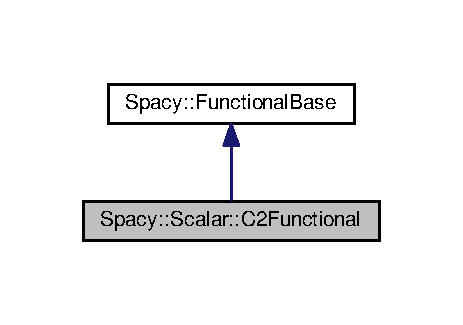
\includegraphics[width=222pt]{classSpacy_1_1Scalar_1_1C2Functional__inherit__graph}
\end{center}
\end{figure}


\-Collaboration diagram for \-Spacy\-:\-:\-Scalar\-:\-:\-C2\-Functional\-:
\nopagebreak
\begin{figure}[H]
\begin{center}
\leavevmode
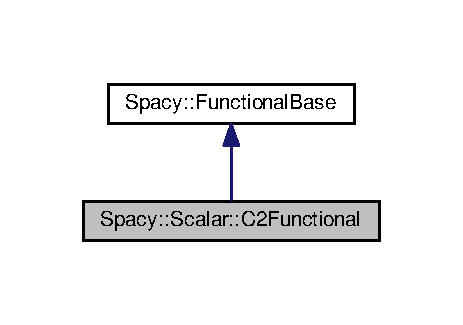
\includegraphics[width=222pt]{classSpacy_1_1Scalar_1_1C2Functional__coll__graph}
\end{center}
\end{figure}
\subsection*{\-Public \-Member \-Functions}
\begin{DoxyCompactItemize}
\item 
\hypertarget{classSpacy_1_1Scalar_1_1C2Functional_a6458c77ba0a55aace7bd3e739078b25b}{{\bfseries \-C2\-Functional} (std\-::function$<$ double(double)$>$ value, std\-::function$<$ double(double)$>$ \hyperlink{namespaceSpacy_a002fe344fa6d04a6ac59a74ea25fddb6}{derivative}, std\-::function$<$ double(double)$>$ sec\-Derivative)}\label{classSpacy_1_1Scalar_1_1C2Functional_a6458c77ba0a55aace7bd3e739078b25b}

\item 
\hypertarget{classSpacy_1_1Scalar_1_1C2Functional_a925d8325d3d58de9ccf82fb4c20a7f87}{\hyperlink{classSpacy_1_1Real}{\-Spacy\-::\-Real} {\bfseries operator()} (const \-::\hyperlink{classSpacy_1_1Vector}{\-Spacy\-::\-Vector} \&x) const }\label{classSpacy_1_1Scalar_1_1C2Functional_a925d8325d3d58de9ccf82fb4c20a7f87}

\item 
\hypertarget{classSpacy_1_1Scalar_1_1C2Functional_ac6baf3f5a3e1fbb1a2dc8172b0d471d5}{\hyperlink{classSpacy_1_1Vector}{\-Spacy\-::\-Vector} {\bfseries d1} (const \-::\hyperlink{classSpacy_1_1Vector}{\-Spacy\-::\-Vector} \&x) const }\label{classSpacy_1_1Scalar_1_1C2Functional_ac6baf3f5a3e1fbb1a2dc8172b0d471d5}

\item 
\hypertarget{classSpacy_1_1Scalar_1_1C2Functional_adcb4d9ed480a86199c82f1d1a97fe6dc}{\hyperlink{classSpacy_1_1Vector}{\-Spacy\-::\-Vector} {\bfseries d2} (const \-::\hyperlink{classSpacy_1_1Vector}{\-Spacy\-::\-Vector} \&x, const \-::\hyperlink{classSpacy_1_1Vector}{\-Spacy\-::\-Vector} \&dx) const }\label{classSpacy_1_1Scalar_1_1C2Functional_adcb4d9ed480a86199c82f1d1a97fe6dc}

\item 
\hypertarget{classSpacy_1_1Scalar_1_1C2Functional_aee5a5f9a601aa339c67ec57e44806343}{\hyperlink{structSpacy_1_1Scalar_1_1LinearOperator}{\-Spacy\-::\-Scalar\-::\-Linear\-Operator} {\bfseries hessian} (const \-::\hyperlink{classSpacy_1_1Vector}{\-Spacy\-::\-Vector} \&x) const }\label{classSpacy_1_1Scalar_1_1C2Functional_aee5a5f9a601aa339c67ec57e44806343}

\item 
\hypertarget{classSpacy_1_1FunctionalBase_a2d3397deb9fa1ad85ed04e37a03b3aa6}{const \hyperlink{classSpacy_1_1VectorSpace}{\-Vector\-Space} \& \hyperlink{classSpacy_1_1FunctionalBase_a2d3397deb9fa1ad85ed04e37a03b3aa6}{domain} () const }\label{classSpacy_1_1FunctionalBase_a2d3397deb9fa1ad85ed04e37a03b3aa6}

\begin{DoxyCompactList}\small\item\em \-Access domain space $X$. \end{DoxyCompactList}\end{DoxyCompactItemize}


\-The documentation for this class was generated from the following file\-:\begin{DoxyCompactItemize}
\item 
/home/travis/build/spacy-\/dev/\-Spacy/\-Spacy/\-Adapter/\-Scalar/c2\-Functional.\-hh\end{DoxyCompactItemize}

\hypertarget{classSpacy_1_1C2Functional}{\section{Spacy\-:\-:C2\-Functional Class Reference}
\label{classSpacy_1_1C2Functional}\index{Spacy\-::\-C2\-Functional@{Spacy\-::\-C2\-Functional}}
}


Type-\/erased twice differentiable functional $f:\ X \to \mathbb{R} $.  




{\ttfamily \#include $<$c2\-Functional.\-hh$>$}

\subsection*{Public Member Functions}
\begin{DoxyCompactItemize}
\item 
\hypertarget{classSpacy_1_1C2Functional_a5dad5f40836b6f43662db0a01fd32347}{\hyperlink{classSpacy_1_1Real}{Real} \hyperlink{classSpacy_1_1C2Functional_a5dad5f40836b6f43662db0a01fd32347}{operator()} (const \hyperlink{classSpacy_1_1Vector}{Vector} \&x) const }\label{classSpacy_1_1C2Functional_a5dad5f40836b6f43662db0a01fd32347}

\begin{DoxyCompactList}\small\item\em Apply functional. \end{DoxyCompactList}\item 
\hypertarget{classSpacy_1_1C2Functional_a7278ddf3337cc28d138a02d18ad44404}{\hyperlink{classSpacy_1_1Vector}{Vector} \hyperlink{classSpacy_1_1C2Functional_a7278ddf3337cc28d138a02d18ad44404}{d1} (const \hyperlink{classSpacy_1_1Vector}{Vector} \&x) const }\label{classSpacy_1_1C2Functional_a7278ddf3337cc28d138a02d18ad44404}

\begin{DoxyCompactList}\small\item\em Compute derivative as function space element in $X^*$, where $x\in X$. \end{DoxyCompactList}\item 
\hypertarget{classSpacy_1_1C2Functional_af2f8671e8ebb9079255afc39a495859d}{\hyperlink{classSpacy_1_1Vector}{Vector} \hyperlink{classSpacy_1_1C2Functional_af2f8671e8ebb9079255afc39a495859d}{d2} (const \hyperlink{classSpacy_1_1Vector}{Vector} \&x, const \hyperlink{classSpacy_1_1Vector}{Vector} \&dx) const }\label{classSpacy_1_1C2Functional_af2f8671e8ebb9079255afc39a495859d}

\begin{DoxyCompactList}\small\item\em Compute second derivative as function space element in $X^*$, where $x,dx\in X$. \end{DoxyCompactList}\item 
\hypertarget{classSpacy_1_1C2Functional_a97eeeb376ed178ea7e2f109967f99c24}{\hyperlink{classSpacy_1_1LinearOperator}{Linear\-Operator} \hyperlink{classSpacy_1_1C2Functional_a97eeeb376ed178ea7e2f109967f99c24}{hessian} (const \hyperlink{classSpacy_1_1Vector}{Vector} \&x) const }\label{classSpacy_1_1C2Functional_a97eeeb376ed178ea7e2f109967f99c24}

\begin{DoxyCompactList}\small\item\em Access hessian as linear operator $ X \rightarrow X^* $. \end{DoxyCompactList}\item 
\hypertarget{classSpacy_1_1C2Functional_ac75246c876b8bf75cdd4f1264bdb49ae}{const \hyperlink{classSpacy_1_1VectorSpace}{Vector\-Space} \& \hyperlink{classSpacy_1_1C2Functional_ac75246c876b8bf75cdd4f1264bdb49ae}{domain} () const }\label{classSpacy_1_1C2Functional_ac75246c876b8bf75cdd4f1264bdb49ae}

\begin{DoxyCompactList}\small\item\em Access domain space $X$. \end{DoxyCompactList}\item 
\hypertarget{classSpacy_1_1C2Functional_ab6c458ef1a423c05f4996717f3772206}{{\footnotesize template$<$class T , typename std\-::enable\-\_\-if$<$ C2\-Functional\-Detail\-::\-Concept$<$ C2\-Functional, typename std\-::decay$<$ T $>$\-::type $>$\-::value $>$\-::type $\ast$  = nullptr$>$ }\\{\bfseries C2\-Functional} (T \&\&value)}\label{classSpacy_1_1C2Functional_ab6c458ef1a423c05f4996717f3772206}

\item 
\hypertarget{classSpacy_1_1C2Functional_a587d2b41ecaa5db9873b2ea8dca604c7}{{\bfseries impl\-\_\-} (std\-::forward$<$ T $>$(value))}\label{classSpacy_1_1C2Functional_a587d2b41ecaa5db9873b2ea8dca604c7}

\item 
\hypertarget{classSpacy_1_1C2Functional_ae5810a028be906128a2c982540fbbcae}{{\footnotesize template$<$class T , typename std\-::enable\-\_\-if$<$ C2\-Functional\-Detail\-::\-Concept$<$ C2\-Functional, typename std\-::decay$<$ T $>$\-::type $>$\-::value $>$\-::type $\ast$  = nullptr$>$ }\\\hyperlink{classSpacy_1_1C2Functional}{C2\-Functional} \& {\bfseries operator=} (T \&\&value)}\label{classSpacy_1_1C2Functional_ae5810a028be906128a2c982540fbbcae}

\item 
\hypertarget{classSpacy_1_1C2Functional_a7305181d522d504c75c0647737fe7d15}{{\bfseries operator bool} () const noexcept}\label{classSpacy_1_1C2Functional_a7305181d522d504c75c0647737fe7d15}

\item 
\hypertarget{classSpacy_1_1C2Functional_a5dad5f40836b6f43662db0a01fd32347}{\hyperlink{classSpacy_1_1Real}{Real} \hyperlink{classSpacy_1_1C2Functional_a5dad5f40836b6f43662db0a01fd32347}{operator()} (const \hyperlink{classSpacy_1_1Vector}{Vector} \&x) const }\label{classSpacy_1_1C2Functional_a5dad5f40836b6f43662db0a01fd32347}

\begin{DoxyCompactList}\small\item\em Apply functional. \end{DoxyCompactList}\item 
\hypertarget{classSpacy_1_1C2Functional_a7278ddf3337cc28d138a02d18ad44404}{\hyperlink{classSpacy_1_1Vector}{Vector} \hyperlink{classSpacy_1_1C2Functional_a7278ddf3337cc28d138a02d18ad44404}{d1} (const \hyperlink{classSpacy_1_1Vector}{Vector} \&x) const }\label{classSpacy_1_1C2Functional_a7278ddf3337cc28d138a02d18ad44404}

\begin{DoxyCompactList}\small\item\em Compute derivative as function space element in $X^*$, where $x\in X$. \end{DoxyCompactList}\item 
\hypertarget{classSpacy_1_1C2Functional_af2f8671e8ebb9079255afc39a495859d}{\hyperlink{classSpacy_1_1Vector}{Vector} \hyperlink{classSpacy_1_1C2Functional_af2f8671e8ebb9079255afc39a495859d}{d2} (const \hyperlink{classSpacy_1_1Vector}{Vector} \&x, const \hyperlink{classSpacy_1_1Vector}{Vector} \&dx) const }\label{classSpacy_1_1C2Functional_af2f8671e8ebb9079255afc39a495859d}

\begin{DoxyCompactList}\small\item\em Compute second derivative as function space element in $X^*$, where $x,dx\in X$. \end{DoxyCompactList}\item 
\hypertarget{classSpacy_1_1C2Functional_a97eeeb376ed178ea7e2f109967f99c24}{\hyperlink{classSpacy_1_1LinearOperator}{Linear\-Operator} \hyperlink{classSpacy_1_1C2Functional_a97eeeb376ed178ea7e2f109967f99c24}{hessian} (const \hyperlink{classSpacy_1_1Vector}{Vector} \&x) const }\label{classSpacy_1_1C2Functional_a97eeeb376ed178ea7e2f109967f99c24}

\begin{DoxyCompactList}\small\item\em Access hessian as linear operator $ X \rightarrow X^$. \end{DoxyCompactList}\item 
\hypertarget{classSpacy_1_1C2Functional_ac75246c876b8bf75cdd4f1264bdb49ae}{const \hyperlink{classSpacy_1_1VectorSpace}{Vector\-Space} \& \hyperlink{classSpacy_1_1C2Functional_ac75246c876b8bf75cdd4f1264bdb49ae}{domain} () const }\label{classSpacy_1_1C2Functional_ac75246c876b8bf75cdd4f1264bdb49ae}

\begin{DoxyCompactList}\small\item\em Access domain space $X$. \end{DoxyCompactList}\item 
\hypertarget{classSpacy_1_1C2Functional_aa1b2f29e86d728629683ebafeb1aa684}{{\footnotesize template$<$class T $>$ }\\T $\ast$ {\bfseries target} () noexcept}\label{classSpacy_1_1C2Functional_aa1b2f29e86d728629683ebafeb1aa684}

\item 
\hypertarget{classSpacy_1_1C2Functional_a26cabef07e8fe8b678d43a98cb2b41e9}{{\footnotesize template$<$class T $>$ }\\const T $\ast$ {\bfseries target} () const noexcept}\label{classSpacy_1_1C2Functional_a26cabef07e8fe8b678d43a98cb2b41e9}

\end{DoxyCompactItemize}


\subsection{Detailed Description}
Type-\/erased twice differentiable functional $f:\ X \to \mathbb{R} $. 

The documentation for this class was generated from the following file\-:\begin{DoxyCompactItemize}
\item 
/home/travis/build/spacy-\/dev/\-Spacy/\-Interfaces/c2\-Functional.\-hh\end{DoxyCompactItemize}

\hypertarget{classSpacy_1_1Rn_1_1C2Functional}{}\section{Spacy\+:\+:Rn\+:\+:C2\+Functional Class Reference}
\label{classSpacy_1_1Rn_1_1C2Functional}\index{Spacy\+::\+Rn\+::\+C2\+Functional@{Spacy\+::\+Rn\+::\+C2\+Functional}}


Inheritance diagram for Spacy\+:\+:Rn\+:\+:C2\+Functional\+:
\nopagebreak
\begin{figure}[H]
\begin{center}
\leavevmode
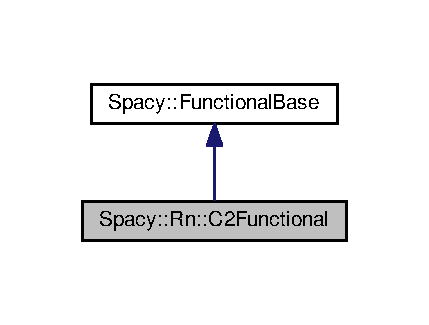
\includegraphics[width=207pt]{classSpacy_1_1Rn_1_1C2Functional__inherit__graph}
\end{center}
\end{figure}


Collaboration diagram for Spacy\+:\+:Rn\+:\+:C2\+Functional\+:
\nopagebreak
\begin{figure}[H]
\begin{center}
\leavevmode
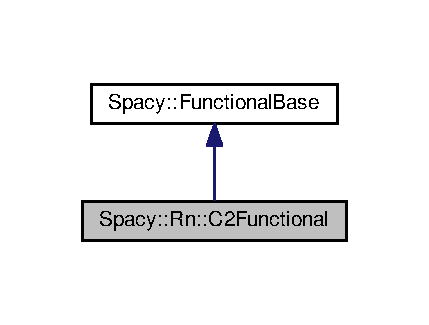
\includegraphics[width=207pt]{classSpacy_1_1Rn_1_1C2Functional__coll__graph}
\end{center}
\end{figure}
\subsection*{Public Member Functions}
\begin{DoxyCompactItemize}
\item 
{\bfseries C2\+Functional} (std\+::function$<$ double(const \+::Eigen\+::\+Vector\+Xd \&)$>$ f, std\+::function$<$ \+::Eigen\+::\+Vector\+Xd(const \+::Eigen\+::\+Vector\+Xd \&) $>$ df, std\+::function$<$ \+::Eigen\+::\+Matrix\+Xd(const \+::Eigen\+::\+Vector\+Xd \&) $>$ ddf, const \hyperlink{classSpacy_1_1VectorSpace}{Vector\+Space} \&\hyperlink{classSpacy_1_1FunctionalBase_a2d3397deb9fa1ad85ed04e37a03b3aa6}{domain})\hypertarget{classSpacy_1_1Rn_1_1C2Functional_a6d17f9e30a1c0fb522a0a135de96f72a}{}\label{classSpacy_1_1Rn_1_1C2Functional_a6d17f9e30a1c0fb522a0a135de96f72a}

\item 
\hyperlink{classSpacy_1_1Real}{Spacy\+::\+Real} {\bfseries operator()} (const \+::\hyperlink{classSpacy_1_1Vector}{Spacy\+::\+Vector} \&x) const \hypertarget{classSpacy_1_1Rn_1_1C2Functional_ad69e7f55b9647b34f6e132e7c831c46f}{}\label{classSpacy_1_1Rn_1_1C2Functional_ad69e7f55b9647b34f6e132e7c831c46f}

\item 
\hyperlink{classSpacy_1_1Vector}{Spacy\+::\+Vector} {\bfseries d1} (const \+::\hyperlink{classSpacy_1_1Vector}{Spacy\+::\+Vector} \&x) const \hypertarget{classSpacy_1_1Rn_1_1C2Functional_a5bfa18cf358557d1d1cc3d2a76022660}{}\label{classSpacy_1_1Rn_1_1C2Functional_a5bfa18cf358557d1d1cc3d2a76022660}

\item 
\hyperlink{classSpacy_1_1Vector}{Spacy\+::\+Vector} {\bfseries d2} (const \+::\hyperlink{classSpacy_1_1Vector}{Spacy\+::\+Vector} \&x, const \+::\hyperlink{classSpacy_1_1Vector}{Spacy\+::\+Vector} \&dx) const \hypertarget{classSpacy_1_1Rn_1_1C2Functional_a4ebc4d850e0c11707a9d4c14f085e920}{}\label{classSpacy_1_1Rn_1_1C2Functional_a4ebc4d850e0c11707a9d4c14f085e920}

\item 
\hyperlink{classSpacy_1_1Rn_1_1LinearOperator}{Linear\+Operator} {\bfseries hessian} (const \+::\hyperlink{classSpacy_1_1Vector}{Spacy\+::\+Vector} \&x) const \hypertarget{classSpacy_1_1Rn_1_1C2Functional_a81b74f77f5680529d82cebde572643e4}{}\label{classSpacy_1_1Rn_1_1C2Functional_a81b74f77f5680529d82cebde572643e4}

\item 
const \hyperlink{classSpacy_1_1VectorSpace}{Vector\+Space} \& \hyperlink{classSpacy_1_1FunctionalBase_a2d3397deb9fa1ad85ed04e37a03b3aa6}{domain} () const \hypertarget{classSpacy_1_1FunctionalBase_a2d3397deb9fa1ad85ed04e37a03b3aa6}{}\label{classSpacy_1_1FunctionalBase_a2d3397deb9fa1ad85ed04e37a03b3aa6}

\begin{DoxyCompactList}\small\item\em Access domain space $X$. \end{DoxyCompactList}\end{DoxyCompactItemize}


The documentation for this class was generated from the following file\+:\begin{DoxyCompactItemize}
\item 
/home/lars/tmp/\+Spacy/\+Spacy/\+Adapter/\+Eigen/c2\+Functional.\+hh\end{DoxyCompactItemize}

\hypertarget{classSpacy_1_1FEniCS_1_1C2Functional}{}\section{Spacy\+:\+:F\+Eni\+CS\+:\+:C2\+Functional$<$ F, DF, D\+DF $>$ Class Template Reference}
\label{classSpacy_1_1FEniCS_1_1C2Functional}\index{Spacy\+::\+F\+Eni\+C\+S\+::\+C2\+Functional$<$ F, D\+F, D\+D\+F $>$@{Spacy\+::\+F\+Eni\+C\+S\+::\+C2\+Functional$<$ F, D\+F, D\+D\+F $>$}}


Functional interface for F\+Eni\+CS. Models a twice differentiable functional $f:X\rightarrow \mathbb{R}$.  




{\ttfamily \#include $<$c2\+Functional.\+hh$>$}



Inheritance diagram for Spacy\+:\+:F\+Eni\+CS\+:\+:C2\+Functional$<$ F, DF, D\+DF $>$\+:
\nopagebreak
\begin{figure}[H]
\begin{center}
\leavevmode
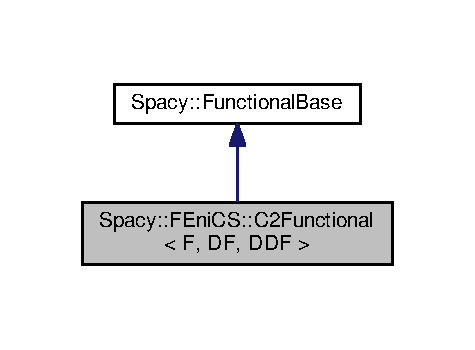
\includegraphics[width=229pt]{classSpacy_1_1FEniCS_1_1C2Functional__inherit__graph}
\end{center}
\end{figure}


Collaboration diagram for Spacy\+:\+:F\+Eni\+CS\+:\+:C2\+Functional$<$ F, DF, D\+DF $>$\+:
\nopagebreak
\begin{figure}[H]
\begin{center}
\leavevmode
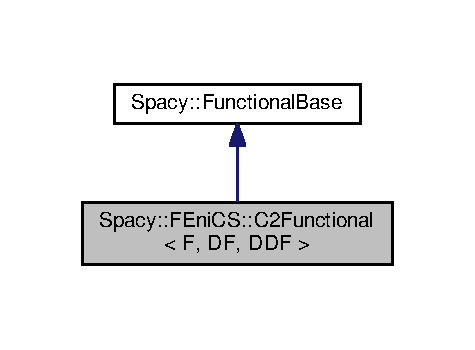
\includegraphics[width=229pt]{classSpacy_1_1FEniCS_1_1C2Functional__coll__graph}
\end{center}
\end{figure}
\subsection*{Public Member Functions}
\begin{DoxyCompactItemize}
\item 
\hyperlink{classSpacy_1_1FEniCS_1_1C2Functional_a8f32c233a72dc3d25a656c1db12af943}{C2\+Functional} (const F \&f, const DF \&J, const D\+DF \&H, const std\+::vector$<$ const dolfin\+::\+Dirichlet\+BC $\ast$ $>$ \&bcs, const \hyperlink{classSpacy_1_1VectorSpace}{Vector\+Space} \&\hyperlink{classSpacy_1_1FunctionalBase_a2d3397deb9fa1ad85ed04e37a03b3aa6}{domain})
\begin{DoxyCompactList}\small\item\em Construct functional for F\+Enics. \end{DoxyCompactList}\item 
\hyperlink{classSpacy_1_1FEniCS_1_1C2Functional_addb84a06f7f82969c57e5bf1b65f2b68}{C2\+Functional} (const \hyperlink{classSpacy_1_1FEniCS_1_1C2Functional}{C2\+Functional} \&g)
\begin{DoxyCompactList}\small\item\em Copy constructor. \end{DoxyCompactList}\item 
\hyperlink{classSpacy_1_1FEniCS_1_1C2Functional}{C2\+Functional} \& \hyperlink{classSpacy_1_1FEniCS_1_1C2Functional_ab9ff23de1e812f6782b7db6ec01e0f4c}{operator=} (const \hyperlink{classSpacy_1_1FEniCS_1_1C2Functional}{C2\+Functional} \&g)
\begin{DoxyCompactList}\small\item\em Copy assignment. \end{DoxyCompactList}\item 
\hyperlink{classSpacy_1_1FEniCS_1_1C2Functional_af9ac63335fc062d18e08fa186312b5a2}{C2\+Functional} (\hyperlink{classSpacy_1_1FEniCS_1_1C2Functional}{C2\+Functional} \&\&g)
\begin{DoxyCompactList}\small\item\em Move constructor. \end{DoxyCompactList}\item 
\hyperlink{classSpacy_1_1FEniCS_1_1C2Functional}{C2\+Functional} \& \hyperlink{classSpacy_1_1FEniCS_1_1C2Functional_a96a909732f7f098d67ee5eba20406337}{operator=} (\hyperlink{classSpacy_1_1FEniCS_1_1C2Functional}{C2\+Functional} \&\&g)
\begin{DoxyCompactList}\small\item\em Move assignment. \end{DoxyCompactList}\item 
\hyperlink{classSpacy_1_1Real}{Real} \hyperlink{classSpacy_1_1FEniCS_1_1C2Functional_abbf25dfc8e8c40edd3ac2dfb61030599}{operator()} (const \+::\hyperlink{classSpacy_1_1Vector}{Spacy\+::\+Vector} \&x) const 
\begin{DoxyCompactList}\small\item\em Apply functional. \end{DoxyCompactList}\item 
\+::\hyperlink{classSpacy_1_1Vector}{Spacy\+::\+Vector} \hyperlink{classSpacy_1_1FEniCS_1_1C2Functional_ab9b10dc982f81093c3125027b46c5876}{d1} (const \+::\hyperlink{classSpacy_1_1Vector}{Spacy\+::\+Vector} \&x) const 
\begin{DoxyCompactList}\small\item\em Compute first directional derivative $f'(x) \in X^* $. \end{DoxyCompactList}\item 
\+::\hyperlink{classSpacy_1_1Vector}{Spacy\+::\+Vector} \hyperlink{classSpacy_1_1FEniCS_1_1C2Functional_affc6728db99f20f57ce75f16799084b4}{d2} (const \+::\hyperlink{classSpacy_1_1Vector}{Spacy\+::\+Vector} \&x, const \+::\hyperlink{classSpacy_1_1Vector}{Spacy\+::\+Vector} \&dx) const 
\begin{DoxyCompactList}\small\item\em Compute second directional derivative $f''(x)dx\in X^* $. \end{DoxyCompactList}\item 
auto \hyperlink{classSpacy_1_1FEniCS_1_1C2Functional_aceec6783f701e121b35ffa482629e1dd}{hessian} (const \+::\hyperlink{classSpacy_1_1Vector}{Spacy\+::\+Vector} \&x) const 
\begin{DoxyCompactList}\small\item\em Access $f''(x)$ as linear operator $X\rightarrow X^*$. \end{DoxyCompactList}\item 
const \hyperlink{classSpacy_1_1VectorSpace}{Vector\+Space} \& \hyperlink{classSpacy_1_1FunctionalBase_a2d3397deb9fa1ad85ed04e37a03b3aa6}{domain} () const \hypertarget{classSpacy_1_1FunctionalBase_a2d3397deb9fa1ad85ed04e37a03b3aa6}{}\label{classSpacy_1_1FunctionalBase_a2d3397deb9fa1ad85ed04e37a03b3aa6}

\begin{DoxyCompactList}\small\item\em Access domain space $X$. \end{DoxyCompactList}\end{DoxyCompactItemize}


\subsection{Detailed Description}
\subsubsection*{template$<$class F, class DF, class D\+DF$>$\\*
class Spacy\+::\+F\+Eni\+C\+S\+::\+C2\+Functional$<$ F, D\+F, D\+D\+F $>$}

Functional interface for F\+Eni\+CS. Models a twice differentiable functional $f:X\rightarrow \mathbb{R}$. 


\begin{DoxyTemplParams}{Template Parameters}
{\em F} & dolfin\+::\+Form describing the functional value \\
\hline
{\em DF} & dolfin\+::\+Form describing the derivative \\
\hline
{\em D\+DF} & dolfin\+::\+Form describing the second derivative \\
\hline
\end{DoxyTemplParams}
\begin{DoxyWarning}{Warning}
In the .ufl file you have to name the argument of $f$ by \char`\"{}x\char`\"{}! 
\end{DoxyWarning}
\begin{DoxySeeAlso}{See also}
\hyperlink{classSpacy_1_1C2Functional}{Spacy\+::\+C2\+Functional} 
\end{DoxySeeAlso}


\subsection{Constructor \& Destructor Documentation}
\index{Spacy\+::\+F\+Eni\+C\+S\+::\+C2\+Functional@{Spacy\+::\+F\+Eni\+C\+S\+::\+C2\+Functional}!C2\+Functional@{C2\+Functional}}
\index{C2\+Functional@{C2\+Functional}!Spacy\+::\+F\+Eni\+C\+S\+::\+C2\+Functional@{Spacy\+::\+F\+Eni\+C\+S\+::\+C2\+Functional}}
\subsubsection[{\texorpdfstring{C2\+Functional(const F \&f, const D\+F \&\+J, const D\+D\+F \&\+H, const std\+::vector$<$ const dolfin\+::\+Dirichlet\+B\+C $\ast$ $>$ \&bcs, const Vector\+Space \&domain)}{C2Functional(const F &f, const DF &J, const DDF &H, const std::vector< const dolfin::DirichletBC * > &bcs, const VectorSpace &domain)}}]{\setlength{\rightskip}{0pt plus 5cm}template$<$class F, class DF, class D\+DF$>$ {\bf Spacy\+::\+F\+Eni\+C\+S\+::\+C2\+Functional}$<$ F, DF, D\+DF $>$\+::{\bf C2\+Functional} (
\begin{DoxyParamCaption}
\item[{const F \&}]{f, }
\item[{const DF \&}]{J, }
\item[{const D\+DF \&}]{H, }
\item[{const std\+::vector$<$ const dolfin\+::\+Dirichlet\+BC $\ast$ $>$ \&}]{bcs, }
\item[{const {\bf Vector\+Space} \&}]{domain}
\end{DoxyParamCaption}
)\hspace{0.3cm}{\ttfamily [inline]}}\hypertarget{classSpacy_1_1FEniCS_1_1C2Functional_a8f32c233a72dc3d25a656c1db12af943}{}\label{classSpacy_1_1FEniCS_1_1C2Functional_a8f32c233a72dc3d25a656c1db12af943}


Construct functional for F\+Enics. 


\begin{DoxyParams}{Parameters}
{\em f} & form for the evaluation of $f$. \\
\hline
{\em J} & form for the evaluation of $f'$ \\
\hline
{\em H} & form for the evaluation of $f''$ \\
\hline
{\em bcs} & Dirichlet boundary conditions \\
\hline
{\em space} & domain space $X$ \\
\hline
\end{DoxyParams}
\index{Spacy\+::\+F\+Eni\+C\+S\+::\+C2\+Functional@{Spacy\+::\+F\+Eni\+C\+S\+::\+C2\+Functional}!C2\+Functional@{C2\+Functional}}
\index{C2\+Functional@{C2\+Functional}!Spacy\+::\+F\+Eni\+C\+S\+::\+C2\+Functional@{Spacy\+::\+F\+Eni\+C\+S\+::\+C2\+Functional}}
\subsubsection[{\texorpdfstring{C2\+Functional(const C2\+Functional \&g)}{C2Functional(const C2Functional &g)}}]{\setlength{\rightskip}{0pt plus 5cm}template$<$class F, class DF, class D\+DF$>$ {\bf Spacy\+::\+F\+Eni\+C\+S\+::\+C2\+Functional}$<$ F, DF, D\+DF $>$\+::{\bf C2\+Functional} (
\begin{DoxyParamCaption}
\item[{const {\bf C2\+Functional}$<$ F, DF, D\+DF $>$ \&}]{g}
\end{DoxyParamCaption}
)\hspace{0.3cm}{\ttfamily [inline]}}\hypertarget{classSpacy_1_1FEniCS_1_1C2Functional_addb84a06f7f82969c57e5bf1b65f2b68}{}\label{classSpacy_1_1FEniCS_1_1C2Functional_addb84a06f7f82969c57e5bf1b65f2b68}


Copy constructor. 


\begin{DoxyParams}{Parameters}
{\em g} & functional to copy from \\
\hline
\end{DoxyParams}
\index{Spacy\+::\+F\+Eni\+C\+S\+::\+C2\+Functional@{Spacy\+::\+F\+Eni\+C\+S\+::\+C2\+Functional}!C2\+Functional@{C2\+Functional}}
\index{C2\+Functional@{C2\+Functional}!Spacy\+::\+F\+Eni\+C\+S\+::\+C2\+Functional@{Spacy\+::\+F\+Eni\+C\+S\+::\+C2\+Functional}}
\subsubsection[{\texorpdfstring{C2\+Functional(\+C2\+Functional \&\&g)}{C2Functional(C2Functional &&g)}}]{\setlength{\rightskip}{0pt plus 5cm}template$<$class F, class DF, class D\+DF$>$ {\bf Spacy\+::\+F\+Eni\+C\+S\+::\+C2\+Functional}$<$ F, DF, D\+DF $>$\+::{\bf C2\+Functional} (
\begin{DoxyParamCaption}
\item[{{\bf C2\+Functional}$<$ F, DF, D\+DF $>$ \&\&}]{g}
\end{DoxyParamCaption}
)\hspace{0.3cm}{\ttfamily [inline]}}\hypertarget{classSpacy_1_1FEniCS_1_1C2Functional_af9ac63335fc062d18e08fa186312b5a2}{}\label{classSpacy_1_1FEniCS_1_1C2Functional_af9ac63335fc062d18e08fa186312b5a2}


Move constructor. 


\begin{DoxyParams}{Parameters}
{\em g} & functional to move from \\
\hline
\end{DoxyParams}


\subsection{Member Function Documentation}
\index{Spacy\+::\+F\+Eni\+C\+S\+::\+C2\+Functional@{Spacy\+::\+F\+Eni\+C\+S\+::\+C2\+Functional}!operator=@{operator=}}
\index{operator=@{operator=}!Spacy\+::\+F\+Eni\+C\+S\+::\+C2\+Functional@{Spacy\+::\+F\+Eni\+C\+S\+::\+C2\+Functional}}
\subsubsection[{\texorpdfstring{operator=(const C2\+Functional \&g)}{operator=(const C2Functional &g)}}]{\setlength{\rightskip}{0pt plus 5cm}template$<$class F, class DF, class D\+DF$>$ {\bf C2\+Functional}\& {\bf Spacy\+::\+F\+Eni\+C\+S\+::\+C2\+Functional}$<$ F, DF, D\+DF $>$\+::operator= (
\begin{DoxyParamCaption}
\item[{const {\bf C2\+Functional}$<$ F, DF, D\+DF $>$ \&}]{g}
\end{DoxyParamCaption}
)\hspace{0.3cm}{\ttfamily [inline]}}\hypertarget{classSpacy_1_1FEniCS_1_1C2Functional_ab9ff23de1e812f6782b7db6ec01e0f4c}{}\label{classSpacy_1_1FEniCS_1_1C2Functional_ab9ff23de1e812f6782b7db6ec01e0f4c}


Copy assignment. 


\begin{DoxyParams}{Parameters}
{\em g} & functional to copy from \\
\hline
\end{DoxyParams}
\index{Spacy\+::\+F\+Eni\+C\+S\+::\+C2\+Functional@{Spacy\+::\+F\+Eni\+C\+S\+::\+C2\+Functional}!operator=@{operator=}}
\index{operator=@{operator=}!Spacy\+::\+F\+Eni\+C\+S\+::\+C2\+Functional@{Spacy\+::\+F\+Eni\+C\+S\+::\+C2\+Functional}}
\subsubsection[{\texorpdfstring{operator=(\+C2\+Functional \&\&g)}{operator=(C2Functional &&g)}}]{\setlength{\rightskip}{0pt plus 5cm}template$<$class F, class DF, class D\+DF$>$ {\bf C2\+Functional}\& {\bf Spacy\+::\+F\+Eni\+C\+S\+::\+C2\+Functional}$<$ F, DF, D\+DF $>$\+::operator= (
\begin{DoxyParamCaption}
\item[{{\bf C2\+Functional}$<$ F, DF, D\+DF $>$ \&\&}]{g}
\end{DoxyParamCaption}
)\hspace{0.3cm}{\ttfamily [inline]}}\hypertarget{classSpacy_1_1FEniCS_1_1C2Functional_a96a909732f7f098d67ee5eba20406337}{}\label{classSpacy_1_1FEniCS_1_1C2Functional_a96a909732f7f098d67ee5eba20406337}


Move assignment. 


\begin{DoxyParams}{Parameters}
{\em g} & functional to move from \\
\hline
\end{DoxyParams}
\index{Spacy\+::\+F\+Eni\+C\+S\+::\+C2\+Functional@{Spacy\+::\+F\+Eni\+C\+S\+::\+C2\+Functional}!operator()@{operator()}}
\index{operator()@{operator()}!Spacy\+::\+F\+Eni\+C\+S\+::\+C2\+Functional@{Spacy\+::\+F\+Eni\+C\+S\+::\+C2\+Functional}}
\subsubsection[{\texorpdfstring{operator()(const \+::\+Spacy\+::\+Vector \&x) const }{operator()(const ::Spacy::Vector &x) const }}]{\setlength{\rightskip}{0pt plus 5cm}template$<$class F, class DF, class D\+DF$>$ {\bf Real} {\bf Spacy\+::\+F\+Eni\+C\+S\+::\+C2\+Functional}$<$ F, DF, D\+DF $>$\+::operator() (
\begin{DoxyParamCaption}
\item[{const \+::{\bf Spacy\+::\+Vector} \&}]{x}
\end{DoxyParamCaption}
) const\hspace{0.3cm}{\ttfamily [inline]}}\hypertarget{classSpacy_1_1FEniCS_1_1C2Functional_abbf25dfc8e8c40edd3ac2dfb61030599}{}\label{classSpacy_1_1FEniCS_1_1C2Functional_abbf25dfc8e8c40edd3ac2dfb61030599}


Apply functional. 


\begin{DoxyParams}{Parameters}
{\em x} & argument \\
\hline
\end{DoxyParams}
\begin{DoxyReturn}{Returns}
$f(x)$ 
\end{DoxyReturn}
\index{Spacy\+::\+F\+Eni\+C\+S\+::\+C2\+Functional@{Spacy\+::\+F\+Eni\+C\+S\+::\+C2\+Functional}!d1@{d1}}
\index{d1@{d1}!Spacy\+::\+F\+Eni\+C\+S\+::\+C2\+Functional@{Spacy\+::\+F\+Eni\+C\+S\+::\+C2\+Functional}}
\subsubsection[{\texorpdfstring{d1(const \+::\+Spacy\+::\+Vector \&x) const }{d1(const ::Spacy::Vector &x) const }}]{\setlength{\rightskip}{0pt plus 5cm}template$<$class F, class DF, class D\+DF$>$ \+::{\bf Spacy\+::\+Vector} {\bf Spacy\+::\+F\+Eni\+C\+S\+::\+C2\+Functional}$<$ F, DF, D\+DF $>$\+::d1 (
\begin{DoxyParamCaption}
\item[{const \+::{\bf Spacy\+::\+Vector} \&}]{x}
\end{DoxyParamCaption}
) const\hspace{0.3cm}{\ttfamily [inline]}}\hypertarget{classSpacy_1_1FEniCS_1_1C2Functional_ab9b10dc982f81093c3125027b46c5876}{}\label{classSpacy_1_1FEniCS_1_1C2Functional_ab9b10dc982f81093c3125027b46c5876}


Compute first directional derivative $f'(x) \in X^* $. 


\begin{DoxyParams}{Parameters}
{\em x} & current iterate \\
\hline
\end{DoxyParams}
\begin{DoxyReturn}{Returns}
$f'(x)$ 
\end{DoxyReturn}
\index{Spacy\+::\+F\+Eni\+C\+S\+::\+C2\+Functional@{Spacy\+::\+F\+Eni\+C\+S\+::\+C2\+Functional}!d2@{d2}}
\index{d2@{d2}!Spacy\+::\+F\+Eni\+C\+S\+::\+C2\+Functional@{Spacy\+::\+F\+Eni\+C\+S\+::\+C2\+Functional}}
\subsubsection[{\texorpdfstring{d2(const \+::\+Spacy\+::\+Vector \&x, const \+::\+Spacy\+::\+Vector \&dx) const }{d2(const ::Spacy::Vector &x, const ::Spacy::Vector &dx) const }}]{\setlength{\rightskip}{0pt plus 5cm}template$<$class F, class DF, class D\+DF$>$ \+::{\bf Spacy\+::\+Vector} {\bf Spacy\+::\+F\+Eni\+C\+S\+::\+C2\+Functional}$<$ F, DF, D\+DF $>$\+::d2 (
\begin{DoxyParamCaption}
\item[{const \+::{\bf Spacy\+::\+Vector} \&}]{x, }
\item[{const \+::{\bf Spacy\+::\+Vector} \&}]{dx}
\end{DoxyParamCaption}
) const\hspace{0.3cm}{\ttfamily [inline]}}\hypertarget{classSpacy_1_1FEniCS_1_1C2Functional_affc6728db99f20f57ce75f16799084b4}{}\label{classSpacy_1_1FEniCS_1_1C2Functional_affc6728db99f20f57ce75f16799084b4}


Compute second directional derivative $f''(x)dx\in X^* $. 


\begin{DoxyParams}{Parameters}
{\em x} & current iterate \\
\hline
{\em dx} & perturbation \\
\hline
\end{DoxyParams}
\begin{DoxyReturn}{Returns}
$f''(x)dx$ 
\end{DoxyReturn}
\index{Spacy\+::\+F\+Eni\+C\+S\+::\+C2\+Functional@{Spacy\+::\+F\+Eni\+C\+S\+::\+C2\+Functional}!hessian@{hessian}}
\index{hessian@{hessian}!Spacy\+::\+F\+Eni\+C\+S\+::\+C2\+Functional@{Spacy\+::\+F\+Eni\+C\+S\+::\+C2\+Functional}}
\subsubsection[{\texorpdfstring{hessian(const \+::\+Spacy\+::\+Vector \&x) const }{hessian(const ::Spacy::Vector &x) const }}]{\setlength{\rightskip}{0pt plus 5cm}template$<$class F, class DF, class D\+DF$>$ auto {\bf Spacy\+::\+F\+Eni\+C\+S\+::\+C2\+Functional}$<$ F, DF, D\+DF $>$\+::hessian (
\begin{DoxyParamCaption}
\item[{const \+::{\bf Spacy\+::\+Vector} \&}]{x}
\end{DoxyParamCaption}
) const\hspace{0.3cm}{\ttfamily [inline]}}\hypertarget{classSpacy_1_1FEniCS_1_1C2Functional_aceec6783f701e121b35ffa482629e1dd}{}\label{classSpacy_1_1FEniCS_1_1C2Functional_aceec6783f701e121b35ffa482629e1dd}


Access $f''(x)$ as linear operator $X\rightarrow X^*$. 


\begin{DoxyParams}{Parameters}
{\em x} & point of linearization \\
\hline
\end{DoxyParams}


The documentation for this class was generated from the following file\+:\begin{DoxyCompactItemize}
\item 
/home/lars/tmp/\+Spacy/\+Spacy/\+Adapter/\+F\+Eni\+C\+S/c2\+Functional.\+hh\end{DoxyCompactItemize}

\hypertarget{structSpacy_1_1C2FunctionalDetail_1_1C2FunctionalConcept}{\section{\-Spacy\-:\-:\-C2\-Functional\-Detail\-:\-:\-C2\-Functional\-Concept$<$ \-Impl, \-T, bool $>$ \-Struct \-Template \-Reference}
\label{structSpacy_1_1C2FunctionalDetail_1_1C2FunctionalConcept}\index{\-Spacy\-::\-C2\-Functional\-Detail\-::\-C2\-Functional\-Concept$<$ Impl, T, bool $>$@{\-Spacy\-::\-C2\-Functional\-Detail\-::\-C2\-Functional\-Concept$<$ Impl, T, bool $>$}}
}
\subsubsection*{template$<$class Impl, class T, bool = std\-::is\-\_\-same$<$ Impl, T $>$\-::value$>$ struct Spacy\-::\-C2\-Functional\-Detail\-::\-C2\-Functional\-Concept$<$ Impl, T, bool $>$}



\-The documentation for this struct was generated from the following file\-:\begin{DoxyCompactItemize}
\item 
/home/travis/build/spacy-\/dev/\-Spacy/\-Spacy/\-Detail/details\-\_\-for\-\_\-c2\-Functional.\-hh\end{DoxyCompactItemize}

\hypertarget{structSpacy_1_1C2FunctionalDetail_1_1C2FunctionalConcept_3_01Impl_00_01T_00_01false_01_4}{\section{\-Spacy\-:\-:\-C2\-Functional\-Detail\-:\-:\-C2\-Functional\-Concept$<$ \-Impl, \-T, false $>$ \-Struct \-Template \-Reference}
\label{structSpacy_1_1C2FunctionalDetail_1_1C2FunctionalConcept_3_01Impl_00_01T_00_01false_01_4}\index{\-Spacy\-::\-C2\-Functional\-Detail\-::\-C2\-Functional\-Concept$<$ Impl, T, false $>$@{\-Spacy\-::\-C2\-Functional\-Detail\-::\-C2\-Functional\-Concept$<$ Impl, T, false $>$}}
}


\-Inheritance diagram for \-Spacy\-:\-:\-C2\-Functional\-Detail\-:\-:\-C2\-Functional\-Concept$<$ \-Impl, \-T, false $>$\-:
\nopagebreak
\begin{figure}[H]
\begin{center}
\leavevmode
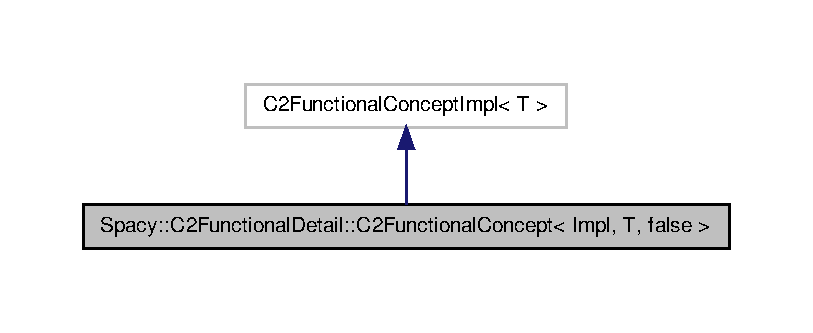
\includegraphics[width=350pt]{structSpacy_1_1C2FunctionalDetail_1_1C2FunctionalConcept_3_01Impl_00_01T_00_01false_01_4__inherit__graph}
\end{center}
\end{figure}


\-Collaboration diagram for \-Spacy\-:\-:\-C2\-Functional\-Detail\-:\-:\-C2\-Functional\-Concept$<$ \-Impl, \-T, false $>$\-:
\nopagebreak
\begin{figure}[H]
\begin{center}
\leavevmode
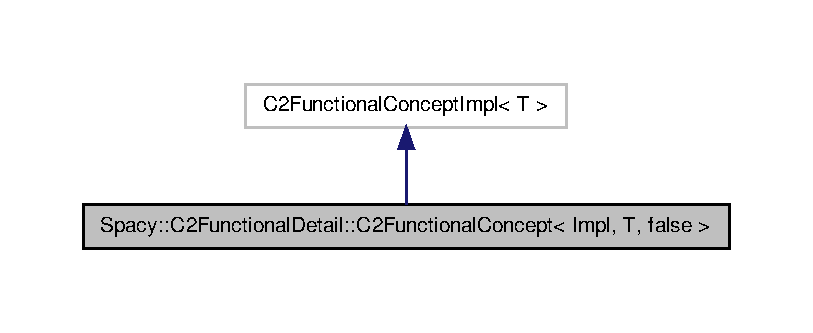
\includegraphics[width=350pt]{structSpacy_1_1C2FunctionalDetail_1_1C2FunctionalConcept_3_01Impl_00_01T_00_01false_01_4__coll__graph}
\end{center}
\end{figure}
\subsubsection*{template$<$class Impl, class T$>$ struct Spacy\-::\-C2\-Functional\-Detail\-::\-C2\-Functional\-Concept$<$ Impl, T, false $>$}



\-The documentation for this struct was generated from the following file\-:\begin{DoxyCompactItemize}
\item 
/home/travis/build/spacy-\/dev/\-Spacy/\-Spacy/\-Detail/details\-\_\-for\-\_\-c2\-Functional.\-hh\end{DoxyCompactItemize}

\hypertarget{classSpacy_1_1CallOfUndefinedFunctionException}{\section{\-Spacy\-:\-:\-Call\-Of\-Undefined\-Function\-Exception \-Class \-Reference}
\label{classSpacy_1_1CallOfUndefinedFunctionException}\index{\-Spacy\-::\-Call\-Of\-Undefined\-Function\-Exception@{\-Spacy\-::\-Call\-Of\-Undefined\-Function\-Exception}}
}


\-Exception to be thrown if a virtual function is not implemented.  




{\ttfamily \#include $<$call\-Of\-Undefined\-Function\-Exception.\-hh$>$}



\-Inheritance diagram for \-Spacy\-:\-:\-Call\-Of\-Undefined\-Function\-Exception\-:
\nopagebreak
\begin{figure}[H]
\begin{center}
\leavevmode
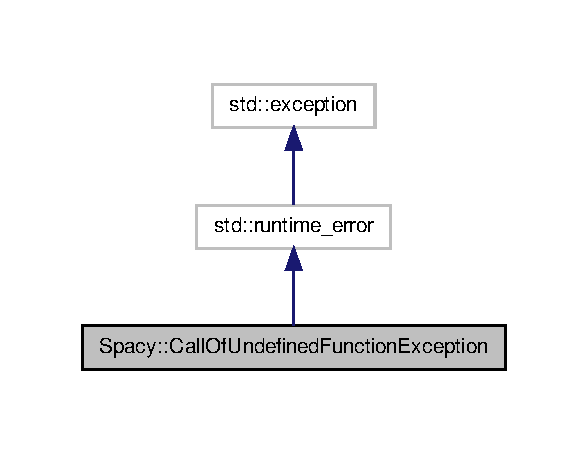
\includegraphics[width=282pt]{classSpacy_1_1CallOfUndefinedFunctionException__inherit__graph}
\end{center}
\end{figure}


\-Collaboration diagram for \-Spacy\-:\-:\-Call\-Of\-Undefined\-Function\-Exception\-:
\nopagebreak
\begin{figure}[H]
\begin{center}
\leavevmode
\includegraphics[width=282pt]{classSpacy_1_1CallOfUndefinedFunctionException__coll__graph}
\end{center}
\end{figure}
\subsection*{\-Public \-Member \-Functions}
\begin{DoxyCompactItemize}
\item 
\hyperlink{classSpacy_1_1CallOfUndefinedFunctionException_ac27ef399db59e2e21d91df93bc84f8c2}{\-Call\-Of\-Undefined\-Function\-Exception} (const std\-::string \&function)
\begin{DoxyCompactList}\small\item\em \-Constructor. \end{DoxyCompactList}\end{DoxyCompactItemize}


\subsection{\-Detailed \-Description}
\-Exception to be thrown if a virtual function is not implemented. 

\subsection{\-Constructor \& \-Destructor \-Documentation}
\hypertarget{classSpacy_1_1CallOfUndefinedFunctionException_ac27ef399db59e2e21d91df93bc84f8c2}{\index{\-Spacy\-::\-Call\-Of\-Undefined\-Function\-Exception@{\-Spacy\-::\-Call\-Of\-Undefined\-Function\-Exception}!\-Call\-Of\-Undefined\-Function\-Exception@{\-Call\-Of\-Undefined\-Function\-Exception}}
\index{\-Call\-Of\-Undefined\-Function\-Exception@{\-Call\-Of\-Undefined\-Function\-Exception}!Spacy::CallOfUndefinedFunctionException@{\-Spacy\-::\-Call\-Of\-Undefined\-Function\-Exception}}
\subsubsection[{\-Call\-Of\-Undefined\-Function\-Exception}]{\setlength{\rightskip}{0pt plus 5cm}{\bf \-Spacy\-::\-Call\-Of\-Undefined\-Function\-Exception\-::\-Call\-Of\-Undefined\-Function\-Exception} (
\begin{DoxyParamCaption}
\item[{const std\-::string \&}]{function}
\end{DoxyParamCaption}
)}}\label{classSpacy_1_1CallOfUndefinedFunctionException_ac27ef399db59e2e21d91df93bc84f8c2}


\-Constructor. 


\begin{DoxyParams}{\-Parameters}
{\em function} & name of function that throws \\
\hline
\end{DoxyParams}


\-The documentation for this class was generated from the following file\-:\begin{DoxyCompactItemize}
\item 
/home/travis/build/spacy-\/dev/\-Spacy/\-Spacy/\-Util/\-Exceptions/call\-Of\-Undefined\-Function\-Exception.\-hh\end{DoxyCompactItemize}

\hypertarget{classSpacy_1_1Kaskade_1_1Lagrange_1_1CGCreator}{\section{\-Spacy\-:\-:\-Kaskade\-:\-:\-Lagrange\-:\-:\-C\-G\-Creator$<$ \-Functional\-Definition, state\-Id, control\-Id, adjoint\-Id $>$ \-Class \-Template \-Reference}
\label{classSpacy_1_1Kaskade_1_1Lagrange_1_1CGCreator}\index{\-Spacy\-::\-Kaskade\-::\-Lagrange\-::\-C\-G\-Creator$<$ Functional\-Definition, state\-Id, control\-Id, adjoint\-Id $>$@{\-Spacy\-::\-Kaskade\-::\-Lagrange\-::\-C\-G\-Creator$<$ Functional\-Definition, state\-Id, control\-Id, adjoint\-Id $>$}}
}


\-Creator for conjugate gradient solver for optimal control problems with a \hyperlink{classSpacy_1_1CG_1_1TriangularStateConstraintPreconditioner}{\-C\-G\-::\-Triangular\-State\-Constraint\-Preconditioner}.  




{\ttfamily \#include $<$lagrange\-C\-G\-Solver.\-hh$>$}



\-Inheritance diagram for \-Spacy\-:\-:\-Kaskade\-:\-:\-Lagrange\-:\-:\-C\-G\-Creator$<$ \-Functional\-Definition, state\-Id, control\-Id, adjoint\-Id $>$\-:
\nopagebreak
\begin{figure}[H]
\begin{center}
\leavevmode
\includegraphics[width=350pt]{classSpacy_1_1Kaskade_1_1Lagrange_1_1CGCreator__inherit__graph}
\end{center}
\end{figure}


\-Collaboration diagram for \-Spacy\-:\-:\-Kaskade\-:\-:\-Lagrange\-:\-:\-C\-G\-Creator$<$ \-Functional\-Definition, state\-Id, control\-Id, adjoint\-Id $>$\-:
\nopagebreak
\begin{figure}[H]
\begin{center}
\leavevmode
\includegraphics[width=350pt]{classSpacy_1_1Kaskade_1_1Lagrange_1_1CGCreator__coll__graph}
\end{center}
\end{figure}
\subsection*{\-Public \-Member \-Functions}
\begin{DoxyCompactItemize}
\item 
\hyperlink{classSpacy_1_1Kaskade_1_1Lagrange_1_1CGCreator_a238054bebf7f15f35b159a3e1804839d}{\-C\-G\-Creator} (std\-::string solver=\char`\"{}\-C\-G\char`\"{})
\begin{DoxyCompactList}\small\item\em \-Constructor. \end{DoxyCompactList}\item 
\-Linear\-Solver \hyperlink{classSpacy_1_1Kaskade_1_1Lagrange_1_1CGCreator_aa9c6be1ff4b871694dc24d026d7d352b}{operator()} (const \hyperlink{classSpacy_1_1Kaskade_1_1C2Functional}{\-C2\-Functional}$<$ \-Functional\-Definition $>$ \&\-L) const 
\begin{DoxyCompactList}\small\item\em \-Create conjugate gradient solver with triangular state constraint preconditioner for $L''$. \end{DoxyCompactList}\item 
\hypertarget{classSpacy_1_1Mixin_1_1Eps_a6b4c38a60848c0ab665fb3a81e181786}{void {\bfseries set\-Eps} (\hyperlink{classSpacy_1_1Real}{\-Real} \hyperlink{classSpacy_1_1Mixin_1_1Eps_a812b99b0abc1d78a34b4114907f23f52}{eps})}\label{classSpacy_1_1Mixin_1_1Eps_a6b4c38a60848c0ab665fb3a81e181786}

\item 
\hypertarget{classSpacy_1_1Mixin_1_1Eps_a812b99b0abc1d78a34b4114907f23f52}{\hyperlink{classSpacy_1_1Real}{\-Real} \hyperlink{classSpacy_1_1Mixin_1_1Eps_a812b99b0abc1d78a34b4114907f23f52}{eps} () const noexcept}\label{classSpacy_1_1Mixin_1_1Eps_a812b99b0abc1d78a34b4114907f23f52}

\begin{DoxyCompactList}\small\item\em \-Access $\varepsilon$. \end{DoxyCompactList}\item 
\hypertarget{classSpacy_1_1Mixin_1_1Eps_abd50a47b32614a950189855775a09d05}{\hyperlink{classSpacy_1_1Real}{\-Real} \hyperlink{classSpacy_1_1Mixin_1_1Eps_abd50a47b32614a950189855775a09d05}{sqrt\-Eps} () const noexcept}\label{classSpacy_1_1Mixin_1_1Eps_abd50a47b32614a950189855775a09d05}

\begin{DoxyCompactList}\small\item\em \-Access $\sqrt\varepsilon$. \end{DoxyCompactList}\item 
\hypertarget{classSpacy_1_1Mixin_1_1Eps_a4bbca3a4afc878d1a20b6335f35e58f7}{\hyperlink{classSpacy_1_1Real}{\-Real} \hyperlink{classSpacy_1_1Mixin_1_1Eps_a4bbca3a4afc878d1a20b6335f35e58f7}{cbrt\-Eps} () const noexcept}\label{classSpacy_1_1Mixin_1_1Eps_a4bbca3a4afc878d1a20b6335f35e58f7}

\begin{DoxyCompactList}\small\item\em \-Access $\varepsilon^{1/3}$. \end{DoxyCompactList}\item 
\hypertarget{classSpacy_1_1Mixin_1_1Eps_a151216968daef3da5f5cdc0b957ce01b}{void \hyperlink{classSpacy_1_1Mixin_1_1Eps_a151216968daef3da5f5cdc0b957ce01b}{update} (\hyperlink{classSpacy_1_1Mixin_1_1Eps_af616ae8e55a645cefd4d2d4504d6705a}{\-Eps} $\ast$changed\-Subject)}\label{classSpacy_1_1Mixin_1_1Eps_a151216968daef3da5f5cdc0b957ce01b}

\begin{DoxyCompactList}\small\item\em update function for observer pattern. \end{DoxyCompactList}\item 
\hypertarget{classSpacy_1_1Mixin_1_1MixinConnection_abb5520ee6b22dd993d78f142939a1ed4}{void \hyperlink{classSpacy_1_1Mixin_1_1MixinConnection_abb5520ee6b22dd993d78f142939a1ed4}{attach} (\hyperlink{classSpacy_1_1Mixin_1_1Eps_af616ae8e55a645cefd4d2d4504d6705a}{\-Eps} \&observer)}\label{classSpacy_1_1Mixin_1_1MixinConnection_abb5520ee6b22dd993d78f142939a1ed4}

\begin{DoxyCompactList}\small\item\em \-Attach observer. \end{DoxyCompactList}\item 
\hypertarget{classSpacy_1_1Mixin_1_1MixinConnection_adda739590c487679c26f60e50aedb73f}{void \hyperlink{classSpacy_1_1Mixin_1_1MixinConnection_adda739590c487679c26f60e50aedb73f}{detach} (\hyperlink{classSpacy_1_1Mixin_1_1Eps_af616ae8e55a645cefd4d2d4504d6705a}{\-Eps} \&observer)}\label{classSpacy_1_1Mixin_1_1MixinConnection_adda739590c487679c26f60e50aedb73f}

\begin{DoxyCompactList}\small\item\em \-Detach observer. \end{DoxyCompactList}\item 
\hypertarget{classSpacy_1_1Mixin_1_1MixinConnection_a1ddeaa78a3bb4a38c2cca36d1f99fe36}{void \hyperlink{classSpacy_1_1Mixin_1_1MixinConnection_a1ddeaa78a3bb4a38c2cca36d1f99fe36}{notify} ()}\label{classSpacy_1_1Mixin_1_1MixinConnection_a1ddeaa78a3bb4a38c2cca36d1f99fe36}

\begin{DoxyCompactList}\small\item\em \-Notify observers about changes. \end{DoxyCompactList}\item 
void \hyperlink{classSpacy_1_1Mixin_1_1Verbosity_a0365d293ab27e27da9496c668020aefb}{set\-Verbosity} (bool \hyperlink{classSpacy_1_1Mixin_1_1Verbosity_ad367a7328578546938fd2a7e52ab3793}{verbose})
\begin{DoxyCompactList}\small\item\em \-Enable/disable verbosity. \end{DoxyCompactList}\item 
\hypertarget{classSpacy_1_1Mixin_1_1Verbosity_ad367a7328578546938fd2a7e52ab3793}{bool \hyperlink{classSpacy_1_1Mixin_1_1Verbosity_ad367a7328578546938fd2a7e52ab3793}{verbose} () const noexcept}\label{classSpacy_1_1Mixin_1_1Verbosity_ad367a7328578546938fd2a7e52ab3793}

\begin{DoxyCompactList}\small\item\em \-Check if verbosity\-Level $>$ 0. \end{DoxyCompactList}\item 
\hypertarget{classSpacy_1_1Mixin_1_1Verbosity_af84a4b3c933f252a5840ab63d4a38325}{void {\bfseries set\-Verbosity\-Level} (unsigned level) noexcept}\label{classSpacy_1_1Mixin_1_1Verbosity_af84a4b3c933f252a5840ab63d4a38325}

\item 
\hypertarget{classSpacy_1_1Mixin_1_1Verbosity_ae55b7493c53b3bb4c2770c99addb5ee1}{unsigned \hyperlink{classSpacy_1_1Mixin_1_1Verbosity_ae55b7493c53b3bb4c2770c99addb5ee1}{get\-Verbosity\-Level} () const noexcept}\label{classSpacy_1_1Mixin_1_1Verbosity_ae55b7493c53b3bb4c2770c99addb5ee1}

\begin{DoxyCompactList}\small\item\em \-Access verbosity level. \end{DoxyCompactList}\item 
\hypertarget{classSpacy_1_1Mixin_1_1Verbosity_a8cff860c587fcda2cdc86ba744302b33}{void \hyperlink{classSpacy_1_1Mixin_1_1Verbosity_a8cff860c587fcda2cdc86ba744302b33}{update} (\hyperlink{classSpacy_1_1Mixin_1_1Verbosity_aefe2f237b0456c4bced001fbfa75f92e}{\-Verbosity} $\ast$changed\-Subject)}\label{classSpacy_1_1Mixin_1_1Verbosity_a8cff860c587fcda2cdc86ba744302b33}

\begin{DoxyCompactList}\small\item\em update function for observer pattern. \end{DoxyCompactList}\item 
\hypertarget{classSpacy_1_1Mixin_1_1MixinConnection_abb5520ee6b22dd993d78f142939a1ed4}{void \hyperlink{classSpacy_1_1Mixin_1_1MixinConnection_abb5520ee6b22dd993d78f142939a1ed4}{attach} (\hyperlink{classSpacy_1_1Mixin_1_1Verbosity_aefe2f237b0456c4bced001fbfa75f92e}{\-Verbosity} \&observer)}\label{classSpacy_1_1Mixin_1_1MixinConnection_abb5520ee6b22dd993d78f142939a1ed4}

\begin{DoxyCompactList}\small\item\em \-Attach observer. \end{DoxyCompactList}\item 
\hypertarget{classSpacy_1_1Mixin_1_1MixinConnection_adda739590c487679c26f60e50aedb73f}{void \hyperlink{classSpacy_1_1Mixin_1_1MixinConnection_adda739590c487679c26f60e50aedb73f}{detach} (\hyperlink{classSpacy_1_1Mixin_1_1Verbosity_aefe2f237b0456c4bced001fbfa75f92e}{\-Verbosity} \&observer)}\label{classSpacy_1_1Mixin_1_1MixinConnection_adda739590c487679c26f60e50aedb73f}

\begin{DoxyCompactList}\small\item\em \-Detach observer. \end{DoxyCompactList}\item 
\hypertarget{classSpacy_1_1Mixin_1_1MixinConnection_a1ddeaa78a3bb4a38c2cca36d1f99fe36}{void \hyperlink{classSpacy_1_1Mixin_1_1MixinConnection_a1ddeaa78a3bb4a38c2cca36d1f99fe36}{notify} ()}\label{classSpacy_1_1Mixin_1_1MixinConnection_a1ddeaa78a3bb4a38c2cca36d1f99fe36}

\begin{DoxyCompactList}\small\item\em \-Notify observers about changes. \end{DoxyCompactList}\end{DoxyCompactItemize}


\subsection{\-Detailed \-Description}
\subsubsection*{template$<$class Functional\-Definition, int state\-Id = 0, int control\-Id = 1, int adjoint\-Id = 2$>$class Spacy\-::\-Kaskade\-::\-Lagrange\-::\-C\-G\-Creator$<$ Functional\-Definition, state\-Id, control\-Id, adjoint\-Id $>$}

\-Creator for conjugate gradient solver for optimal control problems with a \hyperlink{classSpacy_1_1CG_1_1TriangularStateConstraintPreconditioner}{\-C\-G\-::\-Triangular\-State\-Constraint\-Preconditioner}. 

\-Solve a system of the form \[ A = \left( \begin{array}{ccc} L_{yy} & L_{yu} & A^T \\ L_{uy} & L_{uu} & B^T \\ A & B & \end{array} \right)\], with preconditioner \[ P = \left( \begin{array}{ccc} & & A^{-T} \\ & L_{uu}^{-1} & -B^T \\ A^{-1} & -B & \end{array} \right)\], where $A$ is the state operator, $B$ the control operator and $L_{uu}$ is the second derivative of the \-Lagrange functional with respect to the control variable $u$. \-The state variable is denoted by $y$ and the adjoint variable by $p$.


\begin{DoxyTemplParams}{\-Template Parameters}
{\em \-Functional\-Definition} & definition of the \-Lagrange functional from \hyperlink{namespaceSpacy_1_1Kaskade}{\-Kaskade} \\
\hline
{\em state\-Id} & index of the state variable \\
\hline
{\em control\-Id} & index of the control variable \\
\hline
{\em adjoint\-Id} & index of the adjoint variable \\
\hline
\end{DoxyTemplParams}
\begin{DoxySeeAlso}{\-See also}
\hyperlink{classSpacy_1_1CG_1_1Solver}{\-C\-G\-::\-Solver} 
\end{DoxySeeAlso}


\subsection{\-Constructor \& \-Destructor \-Documentation}
\hypertarget{classSpacy_1_1Kaskade_1_1Lagrange_1_1CGCreator_a238054bebf7f15f35b159a3e1804839d}{\index{\-Spacy\-::\-Kaskade\-::\-Lagrange\-::\-C\-G\-Creator@{\-Spacy\-::\-Kaskade\-::\-Lagrange\-::\-C\-G\-Creator}!\-C\-G\-Creator@{\-C\-G\-Creator}}
\index{\-C\-G\-Creator@{\-C\-G\-Creator}!Spacy::Kaskade::Lagrange::CGCreator@{\-Spacy\-::\-Kaskade\-::\-Lagrange\-::\-C\-G\-Creator}}
\subsubsection[{\-C\-G\-Creator}]{\setlength{\rightskip}{0pt plus 5cm}template$<$class Functional\-Definition , int state\-Id = 0, int control\-Id = 1, int adjoint\-Id = 2$>$ {\bf \-Spacy\-::\-Kaskade\-::\-Lagrange\-::\-C\-G\-Creator}$<$ \-Functional\-Definition, state\-Id, control\-Id, adjoint\-Id $>$\-::{\bf \-C\-G\-Creator} (
\begin{DoxyParamCaption}
\item[{std\-::string}]{solver = {\ttfamily \char`\"{}\-C\-G\char`\"{}}}
\end{DoxyParamCaption}
)\hspace{0.3cm}{\ttfamily  \mbox{[}inline, explicit\mbox{]}}}}\label{classSpacy_1_1Kaskade_1_1Lagrange_1_1CGCreator_a238054bebf7f15f35b159a3e1804839d}


\-Constructor. 


\begin{DoxyParams}{\-Parameters}
{\em solver} & solver type (\char`\"{}\-C\-G\char`\"{}, \char`\"{}\-R\-C\-G\char`\"{}, \char`\"{}\-T\-C\-G\char`\"{}, \char`\"{}\-R\-T\-C\-G\char`\"{}). \\
\hline
\end{DoxyParams}
\begin{DoxySeeAlso}{\-See also}
\hyperlink{classSpacy_1_1CG_1_1Solver}{\-C\-G\-::\-Solver} 
\end{DoxySeeAlso}


\subsection{\-Member \-Function \-Documentation}
\hypertarget{classSpacy_1_1Kaskade_1_1Lagrange_1_1CGCreator_aa9c6be1ff4b871694dc24d026d7d352b}{\index{\-Spacy\-::\-Kaskade\-::\-Lagrange\-::\-C\-G\-Creator@{\-Spacy\-::\-Kaskade\-::\-Lagrange\-::\-C\-G\-Creator}!operator()@{operator()}}
\index{operator()@{operator()}!Spacy::Kaskade::Lagrange::CGCreator@{\-Spacy\-::\-Kaskade\-::\-Lagrange\-::\-C\-G\-Creator}}
\subsubsection[{operator()}]{\setlength{\rightskip}{0pt plus 5cm}template$<$class Functional\-Definition , int state\-Id = 0, int control\-Id = 1, int adjoint\-Id = 2$>$ \-Linear\-Solver {\bf \-Spacy\-::\-Kaskade\-::\-Lagrange\-::\-C\-G\-Creator}$<$ \-Functional\-Definition, state\-Id, control\-Id, adjoint\-Id $>$\-::operator() (
\begin{DoxyParamCaption}
\item[{const {\bf \-C2\-Functional}$<$ \-Functional\-Definition $>$ \&}]{\-L}
\end{DoxyParamCaption}
) const\hspace{0.3cm}{\ttfamily  \mbox{[}inline\mbox{]}}}}\label{classSpacy_1_1Kaskade_1_1Lagrange_1_1CGCreator_aa9c6be1ff4b871694dc24d026d7d352b}


\-Create conjugate gradient solver with triangular state constraint preconditioner for $L''$. 


\begin{DoxyParams}{\-Parameters}
{\em \-L} & \-Lagrange functional \\
\hline
\end{DoxyParams}
\begin{DoxyReturn}{\-Returns}
solver representing $L''(x)^{-1}$, where $x$ is the current iterate 
\end{DoxyReturn}
\hypertarget{classSpacy_1_1Mixin_1_1Verbosity_a0365d293ab27e27da9496c668020aefb}{\index{\-Spacy\-::\-Kaskade\-::\-Lagrange\-::\-C\-G\-Creator@{\-Spacy\-::\-Kaskade\-::\-Lagrange\-::\-C\-G\-Creator}!set\-Verbosity@{set\-Verbosity}}
\index{set\-Verbosity@{set\-Verbosity}!Spacy::Kaskade::Lagrange::CGCreator@{\-Spacy\-::\-Kaskade\-::\-Lagrange\-::\-C\-G\-Creator}}
\subsubsection[{set\-Verbosity}]{\setlength{\rightskip}{0pt plus 5cm}void {\bf \-Spacy\-::\-Mixin\-::\-Verbosity\-::set\-Verbosity} (
\begin{DoxyParamCaption}
\item[{bool}]{verbose}
\end{DoxyParamCaption}
)\hspace{0.3cm}{\ttfamily  \mbox{[}inherited\mbox{]}}}}\label{classSpacy_1_1Mixin_1_1Verbosity_a0365d293ab27e27da9496c668020aefb}


\-Enable/disable verbosity. 


\begin{DoxyParams}{\-Parameters}
{\em verbose} & true\-: if verbosity\-Level = 0, set verbosity\-Level = 1; false\-: if set verbosity\-Level = 0 \\
\hline
\end{DoxyParams}


\-The documentation for this class was generated from the following file\-:\begin{DoxyCompactItemize}
\item 
/home/travis/build/spacy-\/dev/\-Spacy/\-Spacy/\-Adapter/\-Kaskade/lagrange\-C\-G\-Solver.\-hh\end{DoxyCompactItemize}

\hypertarget{structSpacy_1_1Kaskade_1_1CoefficientsToVariableSet}{\section{\-Spacy\-:\-:\-Kaskade\-:\-:\-Coefficients\-To\-Variable\-Set$<$ n $>$ \-Struct \-Template \-Reference}
\label{structSpacy_1_1Kaskade_1_1CoefficientsToVariableSet}\index{\-Spacy\-::\-Kaskade\-::\-Coefficients\-To\-Variable\-Set$<$ n $>$@{\-Spacy\-::\-Kaskade\-::\-Coefficients\-To\-Variable\-Set$<$ n $>$}}
}
\subsection*{\-Static \-Public \-Member \-Functions}
\begin{DoxyCompactItemize}
\item 
\hypertarget{structSpacy_1_1Kaskade_1_1CoefficientsToVariableSet_ae781a8e6bdd675c290d92b32c8f365a2}{{\footnotesize template$<$class Coefficient\-Vector , class Variable\-Set $>$ }\\static void {\bfseries apply} (const \-Coefficient\-Vector \&x, \-Variable\-Set \&y)}\label{structSpacy_1_1Kaskade_1_1CoefficientsToVariableSet_ae781a8e6bdd675c290d92b32c8f365a2}

\end{DoxyCompactItemize}
\subsubsection*{template$<$int n$>$ struct Spacy\-::\-Kaskade\-::\-Coefficients\-To\-Variable\-Set$<$ n $>$}



\-The documentation for this struct was generated from the following file\-:\begin{DoxyCompactItemize}
\item 
/home/travis/build/spacy-\/dev/\-Spacy/\-Spacy/\-Adapter/\-Kaskade/util.\-hh\end{DoxyCompactItemize}

\hypertarget{structSpacy_1_1Kaskade_1_1CoefficientsToVariableSet_3-1_01_4}{}\section{Spacy\+:\+:Kaskade\+:\+:Coefficients\+To\+Variable\+Set$<$-\/1 $>$ Struct Template Reference}
\label{structSpacy_1_1Kaskade_1_1CoefficientsToVariableSet_3-1_01_4}\index{Spacy\+::\+Kaskade\+::\+Coefficients\+To\+Variable\+Set$<$-\/1 $>$@{Spacy\+::\+Kaskade\+::\+Coefficients\+To\+Variable\+Set$<$-\/1 $>$}}
\subsection*{Static Public Member Functions}
\begin{DoxyCompactItemize}
\item 
{\footnotesize template$<$class Coefficient\+Vector , class Variable\+Set $>$ }\\static void {\bfseries apply} (const Coefficient\+Vector \&, Variable\+Set \&)\hypertarget{structSpacy_1_1Kaskade_1_1CoefficientsToVariableSet_3-1_01_4_a0cd221cfb9e6fb4d459e2f302a85e743}{}\label{structSpacy_1_1Kaskade_1_1CoefficientsToVariableSet_3-1_01_4_a0cd221cfb9e6fb4d459e2f302a85e743}

\end{DoxyCompactItemize}


The documentation for this struct was generated from the following file\+:\begin{DoxyCompactItemize}
\item 
/home/lars/tmp/\+Spacy/\+Spacy/\+Adapter/\+Kaskade/util.\+hh\end{DoxyCompactItemize}

\hypertarget{classSpacy_1_1Rn_1_1CompositeStepFunctional}{\section{Spacy\-:\-:Rn\-:\-:Composite\-Step\-Functional$<$ role $>$ Class Template Reference}
\label{classSpacy_1_1Rn_1_1CompositeStepFunctional}\index{Spacy\-::\-Rn\-::\-Composite\-Step\-Functional$<$ role $>$@{Spacy\-::\-Rn\-::\-Composite\-Step\-Functional$<$ role $>$}}
}


Inheritance diagram for Spacy\-:\-:Rn\-:\-:Composite\-Step\-Functional$<$ role $>$\-:
\nopagebreak
\begin{figure}[H]
\begin{center}
\leavevmode
\includegraphics[width=216pt]{classSpacy_1_1Rn_1_1CompositeStepFunctional__inherit__graph}
\end{center}
\end{figure}


Collaboration diagram for Spacy\-:\-:Rn\-:\-:Composite\-Step\-Functional$<$ role $>$\-:
\nopagebreak
\begin{figure}[H]
\begin{center}
\leavevmode
\includegraphics[width=216pt]{classSpacy_1_1Rn_1_1CompositeStepFunctional__coll__graph}
\end{center}
\end{figure}
\subsection*{Public Member Functions}
\begin{DoxyCompactItemize}
\item 
\hypertarget{classSpacy_1_1Rn_1_1CompositeStepFunctional_a814c88afc8d4152e1e9bb6fd63b8d211}{{\bfseries Composite\-Step\-Functional} (std\-::function$<$ double(const \-::Eigen\-::\-Vector\-Xd \&)$>$ f, std\-::function$<$ \-::Eigen\-::\-Vector\-Xd(const \-::Eigen\-::\-Vector\-Xd \&) $>$ df, std\-::function$<$ \-::Eigen\-::\-Matrix\-Xd(const \-::Eigen\-::\-Vector\-Xd \&) $>$ ddf, std\-::function$<$ \-::Eigen\-::\-Vector\-Xd(const \-::Eigen\-::\-Vector\-Xd \&) $>$ c, std\-::function$<$ \-::Eigen\-::\-Matrix\-Xd(const \-::Eigen\-::\-Vector\-Xd \&) $>$ dc, std\-::function$<$ \-::Eigen\-::\-Matrix\-Xd(const \-::Eigen\-::\-Vector\-Xd \&, const \-::Eigen\-::\-Vector\-Xd \&) $>$ pddc, const \hyperlink{classSpacy_1_1VectorSpace}{Spacy\-::\-Vector\-Space} \&\hyperlink{classSpacy_1_1FunctionalBase_a2d3397deb9fa1ad85ed04e37a03b3aa6}{domain})}\label{classSpacy_1_1Rn_1_1CompositeStepFunctional_a814c88afc8d4152e1e9bb6fd63b8d211}

\item 
\hypertarget{classSpacy_1_1Rn_1_1CompositeStepFunctional_a3ae8142c85ec8c160e5c2dbc126b20c2}{{\bfseries Composite\-Step\-Functional} (const \hyperlink{classSpacy_1_1Rn_1_1CompositeStepFunctional}{Composite\-Step\-Functional}$<$ Role\-Of\-Functional\-::\-T\-A\-N\-G\-E\-N\-T\-I\-A\-L $>$ \&L\-\_\-\-T, std\-::function$<$ \-::Eigen\-::\-Matrix\-Xd(const \-::Eigen\-::\-Vector\-Xd \&) $>$ M)}\label{classSpacy_1_1Rn_1_1CompositeStepFunctional_a3ae8142c85ec8c160e5c2dbc126b20c2}

\item 
\hypertarget{classSpacy_1_1Rn_1_1CompositeStepFunctional_a4d610559c47b32b4bab04f87376d2f77}{\hyperlink{classSpacy_1_1Real}{Spacy\-::\-Real} {\bfseries operator()} (const \-::\hyperlink{classSpacy_1_1Vector}{Spacy\-::\-Vector} \&x) const }\label{classSpacy_1_1Rn_1_1CompositeStepFunctional_a4d610559c47b32b4bab04f87376d2f77}

\item 
\hypertarget{classSpacy_1_1Rn_1_1CompositeStepFunctional_ad48512ec09d5890e4f50b73e11c69810}{\hyperlink{classSpacy_1_1Vector}{Spacy\-::\-Vector} {\bfseries d1} (const \-::\hyperlink{classSpacy_1_1Vector}{Spacy\-::\-Vector} \&x) const }\label{classSpacy_1_1Rn_1_1CompositeStepFunctional_ad48512ec09d5890e4f50b73e11c69810}

\item 
\hypertarget{classSpacy_1_1Rn_1_1CompositeStepFunctional_aa049e713c6bc06fc271257af31c536c7}{\hyperlink{classSpacy_1_1Vector}{Spacy\-::\-Vector} {\bfseries d2} (const \-::\hyperlink{classSpacy_1_1Vector}{Spacy\-::\-Vector} \&x, const \-::\hyperlink{classSpacy_1_1Vector}{Spacy\-::\-Vector} \&dx) const }\label{classSpacy_1_1Rn_1_1CompositeStepFunctional_aa049e713c6bc06fc271257af31c536c7}

\item 
\hypertarget{classSpacy_1_1Rn_1_1CompositeStepFunctional_a0f406c3e04f4374a2e0bfac66ed99fe8}{\hyperlink{classSpacy_1_1Rn_1_1LinearOperator}{Spacy\-::\-Rn\-::\-Linear\-Operator} {\bfseries hessian} (const \-::\hyperlink{classSpacy_1_1Vector}{Spacy\-::\-Vector} \&x) const }\label{classSpacy_1_1Rn_1_1CompositeStepFunctional_a0f406c3e04f4374a2e0bfac66ed99fe8}

\item 
\hypertarget{classSpacy_1_1FunctionalBase_a2d3397deb9fa1ad85ed04e37a03b3aa6}{const \hyperlink{classSpacy_1_1VectorSpace}{Vector\-Space} \& \hyperlink{classSpacy_1_1FunctionalBase_a2d3397deb9fa1ad85ed04e37a03b3aa6}{domain} () const }\label{classSpacy_1_1FunctionalBase_a2d3397deb9fa1ad85ed04e37a03b3aa6}

\begin{DoxyCompactList}\small\item\em Access domain space $X$. \end{DoxyCompactList}\end{DoxyCompactItemize}
\subsection*{Friends}
\begin{DoxyCompactItemize}
\item 
\hypertarget{classSpacy_1_1Rn_1_1CompositeStepFunctional_ab4d23f390bcf90bf58fd77a6dadc9f7e}{class {\bfseries Composite\-Step\-Functional$<$ Role\-Of\-Functional\-::\-N\-O\-R\-M\-A\-L $>$}}\label{classSpacy_1_1Rn_1_1CompositeStepFunctional_ab4d23f390bcf90bf58fd77a6dadc9f7e}

\end{DoxyCompactItemize}


The documentation for this class was generated from the following file\-:\begin{DoxyCompactItemize}
\item 
/home/travis/build/spacy-\/dev/\-Spacy/\-Spacy/\-Adapter/\-Eigen/composite\-Step\-Functional.\-hh\end{DoxyCompactItemize}

\hypertarget{classSpacy_1_1Mixin_1_1ContractionRate}{\section{\-Spacy\-:\-:\-Mixin\-:\-:\-Contraction\-Rate \-Class \-Reference}
\label{classSpacy_1_1Mixin_1_1ContractionRate}\index{\-Spacy\-::\-Mixin\-::\-Contraction\-Rate@{\-Spacy\-::\-Mixin\-::\-Contraction\-Rate}}
}


\-Mixin class for contraction rates.  




{\ttfamily \#include $<$contraction\-Rate.\-hh$>$}



\-Inheritance diagram for \-Spacy\-:\-:\-Mixin\-:\-:\-Contraction\-Rate\-:
\nopagebreak
\begin{figure}[H]
\begin{center}
\leavevmode
\includegraphics[width=298pt]{classSpacy_1_1Mixin_1_1ContractionRate__inherit__graph}
\end{center}
\end{figure}
\subsection*{\-Public \-Member \-Functions}
\begin{DoxyCompactItemize}
\item 
\hyperlink{classSpacy_1_1Mixin_1_1ContractionRate_a3d6b03823ce3951bafd51ceaac732bf7}{\-Contraction\-Rate} (\hyperlink{classSpacy_1_1Real}{\-Real} desired\-Contraction=0.\-25, \hyperlink{classSpacy_1_1Real}{\-Real} relaxed\-Desired\-Contraction=0.\-5, \hyperlink{classSpacy_1_1Real}{\-Real} maximal\-Contraction=0.\-75) noexcept
\begin{DoxyCompactList}\small\item\em \-Constructor. \end{DoxyCompactList}\item 
\hypertarget{classSpacy_1_1Mixin_1_1ContractionRate_ab9215981f0454bd5d641abad582e64e5}{void {\bfseries set\-Contraction} (\hyperlink{classSpacy_1_1Real}{\-Real} contraction) noexcept}\label{classSpacy_1_1Mixin_1_1ContractionRate_ab9215981f0454bd5d641abad582e64e5}

\item 
\hypertarget{classSpacy_1_1Mixin_1_1ContractionRate_a26eaa6344b5b2191931a9fd87ed96f39}{void {\bfseries set\-Desired\-Contraction} (\hyperlink{classSpacy_1_1Real}{\-Real} desired\-Contraction) noexcept}\label{classSpacy_1_1Mixin_1_1ContractionRate_a26eaa6344b5b2191931a9fd87ed96f39}

\item 
\hypertarget{classSpacy_1_1Mixin_1_1ContractionRate_ac6e47c0ab683643fea7490703f02632d}{void {\bfseries set\-Relaxed\-Desired\-Contraction} (\hyperlink{classSpacy_1_1Real}{\-Real} relaxed\-Desired\-Contraction) noexcept}\label{classSpacy_1_1Mixin_1_1ContractionRate_ac6e47c0ab683643fea7490703f02632d}

\item 
\hypertarget{classSpacy_1_1Mixin_1_1ContractionRate_acc99ba536cd9a027baa50a1412d9d216}{void {\bfseries set\-Maximal\-Contraction} (\hyperlink{classSpacy_1_1Real}{\-Real} maximal\-Contraction) noexcept}\label{classSpacy_1_1Mixin_1_1ContractionRate_acc99ba536cd9a027baa50a1412d9d216}

\item 
\hypertarget{classSpacy_1_1Mixin_1_1ContractionRate_a49a83927f070d2dd600966f491f1f304}{\hyperlink{classSpacy_1_1Real}{\-Real} {\bfseries get\-Contraction} () const noexcept}\label{classSpacy_1_1Mixin_1_1ContractionRate_a49a83927f070d2dd600966f491f1f304}

\item 
\hypertarget{classSpacy_1_1Mixin_1_1ContractionRate_a3704d54e5015a9b7d9cdc2c01f41b205}{\hyperlink{classSpacy_1_1Real}{\-Real} {\bfseries get\-Desired\-Contraction} () const noexcept}\label{classSpacy_1_1Mixin_1_1ContractionRate_a3704d54e5015a9b7d9cdc2c01f41b205}

\item 
\hypertarget{classSpacy_1_1Mixin_1_1ContractionRate_ab2c819795e61d188bf0e35c3206ada8b}{\hyperlink{classSpacy_1_1Real}{\-Real} {\bfseries get\-Relaxed\-Desired\-Contraction} () const noexcept}\label{classSpacy_1_1Mixin_1_1ContractionRate_ab2c819795e61d188bf0e35c3206ada8b}

\item 
\hypertarget{classSpacy_1_1Mixin_1_1ContractionRate_a7b7f42a2263b7bd76db4e9c61a5bc5b1}{\hyperlink{classSpacy_1_1Real}{\-Real} {\bfseries get\-Maximal\-Contraction} () const noexcept}\label{classSpacy_1_1Mixin_1_1ContractionRate_a7b7f42a2263b7bd76db4e9c61a5bc5b1}

\item 
\hypertarget{classSpacy_1_1Mixin_1_1ContractionRate_aeae43593fd23f40159ed9f00a3cde399}{bool {\bfseries contraction\-Is\-Admissible} () const noexcept}\label{classSpacy_1_1Mixin_1_1ContractionRate_aeae43593fd23f40159ed9f00a3cde399}

\end{DoxyCompactItemize}


\subsection{\-Detailed \-Description}
\-Mixin class for contraction rates. 

\subsection{\-Constructor \& \-Destructor \-Documentation}
\hypertarget{classSpacy_1_1Mixin_1_1ContractionRate_a3d6b03823ce3951bafd51ceaac732bf7}{\index{\-Spacy\-::\-Mixin\-::\-Contraction\-Rate@{\-Spacy\-::\-Mixin\-::\-Contraction\-Rate}!\-Contraction\-Rate@{\-Contraction\-Rate}}
\index{\-Contraction\-Rate@{\-Contraction\-Rate}!Spacy::Mixin::ContractionRate@{\-Spacy\-::\-Mixin\-::\-Contraction\-Rate}}
\subsubsection[{\-Contraction\-Rate}]{\setlength{\rightskip}{0pt plus 5cm}{\bf \-Spacy\-::\-Mixin\-::\-Contraction\-Rate\-::\-Contraction\-Rate} (
\begin{DoxyParamCaption}
\item[{{\bf \-Real}}]{desired\-Contraction = {\ttfamily 0.25}, }
\item[{{\bf \-Real}}]{relaxed\-Desired\-Contraction = {\ttfamily 0.5}, }
\item[{{\bf \-Real}}]{maximal\-Contraction = {\ttfamily 0.75}}
\end{DoxyParamCaption}
)\hspace{0.3cm}{\ttfamily  \mbox{[}explicit\mbox{]}}}}\label{classSpacy_1_1Mixin_1_1ContractionRate_a3d6b03823ce3951bafd51ceaac732bf7}


\-Constructor. 


\begin{DoxyParams}{\-Parameters}
{\em desired\-Contraction} & desired contraction rate \\
\hline
{\em relaxed\-Desired\-Contraction} & relaxed contraction rate \\
\hline
{\em maximal\-Contraction} & maximal allowed contraction rate \\
\hline
\end{DoxyParams}


\-The documentation for this class was generated from the following file\-:\begin{DoxyCompactItemize}
\item 
/home/travis/build/spacy-\/dev/\-Spacy/\-Spacy/\-Util/\-Mixins/contraction\-Rate.\-hh\end{DoxyCompactItemize}

\hypertarget{classSpacy_1_1Cubic}{\section{\-Spacy\-:\-:\-Cubic \-Class \-Reference}
\label{classSpacy_1_1Cubic}\index{\-Spacy\-::\-Cubic@{\-Spacy\-::\-Cubic}}
}


\-A one-\/dimensional cubic function $q(t) = a + bt + ct^2 + dt^3$.  




{\ttfamily \#include $<$cubic.\-hh$>$}

\subsection*{\-Public \-Member \-Functions}
\begin{DoxyCompactItemize}
\item 
\hypertarget{classSpacy_1_1Cubic_aa0893e2540b9f5ac4b85e168c1f7d6d4}{{\bfseries \-Cubic} (\hyperlink{classSpacy_1_1Real}{\-Real} a, \hyperlink{classSpacy_1_1Real}{\-Real} b, \hyperlink{classSpacy_1_1Real}{\-Real} c, \hyperlink{classSpacy_1_1Real}{\-Real} d) noexcept}\label{classSpacy_1_1Cubic_aa0893e2540b9f5ac4b85e168c1f7d6d4}

\item 
\hypertarget{classSpacy_1_1Cubic_af2c7cb43b2d55bad525ade5caafe898e}{\hyperlink{classSpacy_1_1Real}{\-Real} \hyperlink{classSpacy_1_1Cubic_af2c7cb43b2d55bad525ade5caafe898e}{operator()} (\hyperlink{classSpacy_1_1Real}{\-Real} t) const noexcept}\label{classSpacy_1_1Cubic_af2c7cb43b2d55bad525ade5caafe898e}

\begin{DoxyCompactList}\small\item\em \-Compute $q(t) = a + bt + ct^2 + dt^3 $. \end{DoxyCompactList}\end{DoxyCompactItemize}


\subsection{\-Detailed \-Description}
\-A one-\/dimensional cubic function $q(t) = a + bt + ct^2 + dt^3$. 

\-The documentation for this class was generated from the following file\-:\begin{DoxyCompactItemize}
\item 
/home/travis/build/spacy-\/dev/\-Spacy/\-Spacy/\-Algorithm/\-Scalar/cubic.\-hh\end{DoxyCompactItemize}

\hypertarget{classSpacy_1_1CompositeStep_1_1CubicModel}{}\section{Spacy\+:\+:Composite\+Step\+:\+:Cubic\+Model Class Reference}
\label{classSpacy_1_1CompositeStep_1_1CubicModel}\index{Spacy\+::\+Composite\+Step\+::\+Cubic\+Model@{Spacy\+::\+Composite\+Step\+::\+Cubic\+Model}}


The cubic regularized model for the affine covariant composite step method of \cite{Lubkoll2015}, \cite{Lubkoll2015a}.  




{\ttfamily \#include $<$quadratic\+Model.\+hh$>$}

\subsection*{Public Member Functions}
\begin{DoxyCompactItemize}
\item 
\hyperlink{classSpacy_1_1CompositeStep_1_1CubicModel_a81bcf7731badd9c540acf9c4ee07b67b}{Cubic\+Model} (const \hyperlink{classSpacy_1_1Quadratic}{Quadratic} \&quadratic\+Model, const \hyperlink{classSpacy_1_1Quadratic}{Quadratic} \&squared\+Norm, double omega)
\begin{DoxyCompactList}\small\item\em Constructor. \end{DoxyCompactList}\item 
\hyperlink{classSpacy_1_1Real}{Real} \hyperlink{classSpacy_1_1CompositeStep_1_1CubicModel_a5669f387117cfdc47b5be45a29f387ce}{operator()} (\hyperlink{classSpacy_1_1Real}{Real} t) const 
\begin{DoxyCompactList}\small\item\em Evaluate cubic model $ q(t) = q_1(t) + \frac{\omega}{6}q_2^{3/2} $. \end{DoxyCompactList}\end{DoxyCompactItemize}


\subsection{Detailed Description}
The cubic regularized model for the affine covariant composite step method of \cite{Lubkoll2015}, \cite{Lubkoll2015a}. 

\subsection{Constructor \& Destructor Documentation}
\index{Spacy\+::\+Composite\+Step\+::\+Cubic\+Model@{Spacy\+::\+Composite\+Step\+::\+Cubic\+Model}!Cubic\+Model@{Cubic\+Model}}
\index{Cubic\+Model@{Cubic\+Model}!Spacy\+::\+Composite\+Step\+::\+Cubic\+Model@{Spacy\+::\+Composite\+Step\+::\+Cubic\+Model}}
\subsubsection[{\texorpdfstring{Cubic\+Model(const Quadratic \&quadratic\+Model, const Quadratic \&squared\+Norm, double omega)}{CubicModel(const Quadratic &quadraticModel, const Quadratic &squaredNorm, double omega)}}]{\setlength{\rightskip}{0pt plus 5cm}Spacy\+::\+Composite\+Step\+::\+Cubic\+Model\+::\+Cubic\+Model (
\begin{DoxyParamCaption}
\item[{const {\bf Quadratic} \&}]{quadratic\+Model, }
\item[{const {\bf Quadratic} \&}]{squared\+Norm, }
\item[{double}]{omega}
\end{DoxyParamCaption}
)}\hypertarget{classSpacy_1_1CompositeStep_1_1CubicModel_a81bcf7731badd9c540acf9c4ee07b67b}{}\label{classSpacy_1_1CompositeStep_1_1CubicModel_a81bcf7731badd9c540acf9c4ee07b67b}


Constructor. 


\begin{DoxyParams}{Parameters}
{\em quadratic\+Model} & quadratic model $q_1$ of the Lagrange functional (generated with make\+Quadratic\+Model(...)) \\
\hline
{\em squared\+Norm} & quadratic model $q_2$ of a norm (generated with make\+Quadratic\+Norm\+Model(...)) \\
\hline
{\em omega} & estimate of the Lipschitz constant of the second derivative of the Lagrangian \\
\hline
\end{DoxyParams}


\subsection{Member Function Documentation}
\index{Spacy\+::\+Composite\+Step\+::\+Cubic\+Model@{Spacy\+::\+Composite\+Step\+::\+Cubic\+Model}!operator()@{operator()}}
\index{operator()@{operator()}!Spacy\+::\+Composite\+Step\+::\+Cubic\+Model@{Spacy\+::\+Composite\+Step\+::\+Cubic\+Model}}
\subsubsection[{\texorpdfstring{operator()(\+Real t) const }{operator()(Real t) const }}]{\setlength{\rightskip}{0pt plus 5cm}{\bf Real} Spacy\+::\+Composite\+Step\+::\+Cubic\+Model\+::operator() (
\begin{DoxyParamCaption}
\item[{{\bf Real}}]{t}
\end{DoxyParamCaption}
) const}\hypertarget{classSpacy_1_1CompositeStep_1_1CubicModel_a5669f387117cfdc47b5be45a29f387ce}{}\label{classSpacy_1_1CompositeStep_1_1CubicModel_a5669f387117cfdc47b5be45a29f387ce}


Evaluate cubic model $ q(t) = q_1(t) + \frac{\omega}{6}q_2^{3/2} $. 


\begin{DoxyParams}{Parameters}
{\em t} & argument \\
\hline
\end{DoxyParams}
\begin{DoxyReturn}{Returns}
$ q(t) = q_1(t) + \frac{\omega}{6}q_2^{3/2} $ 
\end{DoxyReturn}


The documentation for this class was generated from the following file\+:\begin{DoxyCompactItemize}
\item 
/home/lars/tmp/\+Spacy/\+Spacy/\+Algorithm/\+Composite\+Step/quadratic\+Model.\+hh\end{DoxyCompactItemize}

\hypertarget{classSpacy_1_1DampingFactor}{\section{\-Spacy\-:\-:\-Damping\-Factor \-Class \-Reference}
\label{classSpacy_1_1DampingFactor}\index{\-Spacy\-::\-Damping\-Factor@{\-Spacy\-::\-Damping\-Factor}}
}


\-A simple model of a damping factor $\nu$ that is computed up to a prescribed accuracy $\varepsilon$.  




{\ttfamily \#include $<$damping\-Factor.\-hh$>$}



\-Inheritance diagram for \-Spacy\-:\-:\-Damping\-Factor\-:
\nopagebreak
\begin{figure}[H]
\begin{center}
\leavevmode
\includegraphics[width=268pt]{classSpacy_1_1DampingFactor__inherit__graph}
\end{center}
\end{figure}


\-Collaboration diagram for \-Spacy\-:\-:\-Damping\-Factor\-:
\nopagebreak
\begin{figure}[H]
\begin{center}
\leavevmode
\includegraphics[width=268pt]{classSpacy_1_1DampingFactor__coll__graph}
\end{center}
\end{figure}
\subsection*{\-Public \-Member \-Functions}
\begin{DoxyCompactItemize}
\item 
\hyperlink{classSpacy_1_1DampingFactor_a70e93ad9b0245cbc644d0f930d0cadc0}{\-Damping\-Factor} (\hyperlink{classSpacy_1_1Real}{\-Real} nu, \hyperlink{classSpacy_1_1Real}{\-Real} \hyperlink{classSpacy_1_1Mixin_1_1Eps_a812b99b0abc1d78a34b4114907f23f52}{eps}=1e-\/3) noexcept
\begin{DoxyCompactList}\small\item\em \-Constructor. \end{DoxyCompactList}\item 
\hyperlink{classSpacy_1_1DampingFactor}{\-Damping\-Factor} \& \hyperlink{classSpacy_1_1DampingFactor_ae28aa1372882e7cc94ff64e16835e7bd}{operator=} (\hyperlink{classSpacy_1_1Real}{\-Real} nu) noexcept
\begin{DoxyCompactList}\small\item\em \-Set damping factor $\nu$. \end{DoxyCompactList}\item 
\hypertarget{classSpacy_1_1DampingFactor_a58e54413ae9d5a78e90a7f99c58a127a}{\hyperlink{classSpacy_1_1DampingFactor}{\-Damping\-Factor} \& \hyperlink{classSpacy_1_1DampingFactor_a58e54413ae9d5a78e90a7f99c58a127a}{operator$\ast$=} (\hyperlink{classSpacy_1_1Real}{\-Real} value)}\label{classSpacy_1_1DampingFactor_a58e54413ae9d5a78e90a7f99c58a127a}

\begin{DoxyCompactList}\small\item\em \-In-\/place multiplication. \end{DoxyCompactList}\item 
\hypertarget{classSpacy_1_1DampingFactor_ad5f845e6bbf9f232e09aeea07ab4c32e}{\hyperlink{classSpacy_1_1DampingFactor}{\-Damping\-Factor} \hyperlink{classSpacy_1_1DampingFactor_ad5f845e6bbf9f232e09aeea07ab4c32e}{operator-\/} () const noexcept}\label{classSpacy_1_1DampingFactor_ad5f845e6bbf9f232e09aeea07ab4c32e}

\begin{DoxyCompactList}\small\item\em \-Invert damping factor. \end{DoxyCompactList}\item 
\hypertarget{classSpacy_1_1Mixin_1_1Eps_a6b4c38a60848c0ab665fb3a81e181786}{void {\bfseries set\-Eps} (\hyperlink{classSpacy_1_1Real}{\-Real} \hyperlink{classSpacy_1_1Mixin_1_1Eps_a812b99b0abc1d78a34b4114907f23f52}{eps})}\label{classSpacy_1_1Mixin_1_1Eps_a6b4c38a60848c0ab665fb3a81e181786}

\item 
\hypertarget{classSpacy_1_1Mixin_1_1Eps_a812b99b0abc1d78a34b4114907f23f52}{\hyperlink{classSpacy_1_1Real}{\-Real} \hyperlink{classSpacy_1_1Mixin_1_1Eps_a812b99b0abc1d78a34b4114907f23f52}{eps} () const noexcept}\label{classSpacy_1_1Mixin_1_1Eps_a812b99b0abc1d78a34b4114907f23f52}

\begin{DoxyCompactList}\small\item\em \-Access $\varepsilon$. \end{DoxyCompactList}\item 
\hypertarget{classSpacy_1_1Mixin_1_1Eps_abd50a47b32614a950189855775a09d05}{\hyperlink{classSpacy_1_1Real}{\-Real} \hyperlink{classSpacy_1_1Mixin_1_1Eps_abd50a47b32614a950189855775a09d05}{sqrt\-Eps} () const noexcept}\label{classSpacy_1_1Mixin_1_1Eps_abd50a47b32614a950189855775a09d05}

\begin{DoxyCompactList}\small\item\em \-Access $\sqrt\varepsilon$. \end{DoxyCompactList}\item 
\hypertarget{classSpacy_1_1Mixin_1_1Eps_a4bbca3a4afc878d1a20b6335f35e58f7}{\hyperlink{classSpacy_1_1Real}{\-Real} \hyperlink{classSpacy_1_1Mixin_1_1Eps_a4bbca3a4afc878d1a20b6335f35e58f7}{cbrt\-Eps} () const noexcept}\label{classSpacy_1_1Mixin_1_1Eps_a4bbca3a4afc878d1a20b6335f35e58f7}

\begin{DoxyCompactList}\small\item\em \-Access $\varepsilon^{1/3}$. \end{DoxyCompactList}\item 
\hypertarget{classSpacy_1_1Mixin_1_1Eps_a151216968daef3da5f5cdc0b957ce01b}{void \hyperlink{classSpacy_1_1Mixin_1_1Eps_a151216968daef3da5f5cdc0b957ce01b}{update} (\hyperlink{classSpacy_1_1Mixin_1_1Eps_af616ae8e55a645cefd4d2d4504d6705a}{\-Eps} $\ast$changed\-Subject)}\label{classSpacy_1_1Mixin_1_1Eps_a151216968daef3da5f5cdc0b957ce01b}

\begin{DoxyCompactList}\small\item\em update function for observer pattern. \end{DoxyCompactList}\item 
\hypertarget{classSpacy_1_1Mixin_1_1MixinConnection_abb5520ee6b22dd993d78f142939a1ed4}{void \hyperlink{classSpacy_1_1Mixin_1_1MixinConnection_abb5520ee6b22dd993d78f142939a1ed4}{attach} (\hyperlink{classSpacy_1_1Mixin_1_1Eps_af616ae8e55a645cefd4d2d4504d6705a}{\-Eps} \&observer)}\label{classSpacy_1_1Mixin_1_1MixinConnection_abb5520ee6b22dd993d78f142939a1ed4}

\begin{DoxyCompactList}\small\item\em \-Attach observer. \end{DoxyCompactList}\item 
\hypertarget{classSpacy_1_1Mixin_1_1MixinConnection_adda739590c487679c26f60e50aedb73f}{void \hyperlink{classSpacy_1_1Mixin_1_1MixinConnection_adda739590c487679c26f60e50aedb73f}{detach} (\hyperlink{classSpacy_1_1Mixin_1_1Eps_af616ae8e55a645cefd4d2d4504d6705a}{\-Eps} \&observer)}\label{classSpacy_1_1Mixin_1_1MixinConnection_adda739590c487679c26f60e50aedb73f}

\begin{DoxyCompactList}\small\item\em \-Detach observer. \end{DoxyCompactList}\item 
\hypertarget{classSpacy_1_1Mixin_1_1MixinConnection_a1ddeaa78a3bb4a38c2cca36d1f99fe36}{void \hyperlink{classSpacy_1_1Mixin_1_1MixinConnection_a1ddeaa78a3bb4a38c2cca36d1f99fe36}{notify} ()}\label{classSpacy_1_1Mixin_1_1MixinConnection_a1ddeaa78a3bb4a38c2cca36d1f99fe36}

\begin{DoxyCompactList}\small\item\em \-Notify observers about changes. \end{DoxyCompactList}\end{DoxyCompactItemize}


\subsection{\-Detailed \-Description}
\-A simple model of a damping factor $\nu$ that is computed up to a prescribed accuracy $\varepsilon$. 

\subsection{\-Constructor \& \-Destructor \-Documentation}
\hypertarget{classSpacy_1_1DampingFactor_a70e93ad9b0245cbc644d0f930d0cadc0}{\index{\-Spacy\-::\-Damping\-Factor@{\-Spacy\-::\-Damping\-Factor}!\-Damping\-Factor@{\-Damping\-Factor}}
\index{\-Damping\-Factor@{\-Damping\-Factor}!Spacy::DampingFactor@{\-Spacy\-::\-Damping\-Factor}}
\subsubsection[{\-Damping\-Factor}]{\setlength{\rightskip}{0pt plus 5cm}{\bf \-Spacy\-::\-Damping\-Factor\-::\-Damping\-Factor} (
\begin{DoxyParamCaption}
\item[{{\bf \-Real}}]{nu, }
\item[{{\bf \-Real}}]{eps = {\ttfamily 1e-\/3}}
\end{DoxyParamCaption}
)\hspace{0.3cm}{\ttfamily  \mbox{[}explicit\mbox{]}}}}\label{classSpacy_1_1DampingFactor_a70e93ad9b0245cbc644d0f930d0cadc0}


\-Constructor. 


\begin{DoxyParams}{\-Parameters}
{\em nu} & damping factor $\nu$ \\
\hline
{\em eps} & accuracy $\varepsilon$. \\
\hline
\end{DoxyParams}


\subsection{\-Member \-Function \-Documentation}
\hypertarget{classSpacy_1_1DampingFactor_ae28aa1372882e7cc94ff64e16835e7bd}{\index{\-Spacy\-::\-Damping\-Factor@{\-Spacy\-::\-Damping\-Factor}!operator=@{operator=}}
\index{operator=@{operator=}!Spacy::DampingFactor@{\-Spacy\-::\-Damping\-Factor}}
\subsubsection[{operator=}]{\setlength{\rightskip}{0pt plus 5cm}{\bf \-Damping\-Factor}\& \-Spacy\-::\-Damping\-Factor\-::operator= (
\begin{DoxyParamCaption}
\item[{{\bf \-Real}}]{nu}
\end{DoxyParamCaption}
)}}\label{classSpacy_1_1DampingFactor_ae28aa1372882e7cc94ff64e16835e7bd}


\-Set damping factor $\nu$. 

\-If $ |\nu-1| < \varepsilon $ then $\nu$ is set to 1.


\begin{DoxyParams}{\-Parameters}
{\em nu} & damping factor \\
\hline
\end{DoxyParams}


\-The documentation for this class was generated from the following file\-:\begin{DoxyCompactItemize}
\item 
/home/travis/build/spacy-\/dev/\-Spacy/\-Spacy/\-Algorithm/damping\-Factor.\-hh\end{DoxyCompactItemize}

\hypertarget{classSpacy_1_1Mixin_1_1DecreaseCondition}{\section{\-Spacy\-:\-:\-Mixin\-:\-:\-Decrease\-Condition \-Class \-Reference}
\label{classSpacy_1_1Mixin_1_1DecreaseCondition}\index{\-Spacy\-::\-Mixin\-::\-Decrease\-Condition@{\-Spacy\-::\-Mixin\-::\-Decrease\-Condition}}
}


\-Mixin class for accepting local models $m$ of nonlinear optimization problems $\min f(x)$.  




{\ttfamily \#include $<$decrease\-Condition.\-hh$>$}



\-Inheritance diagram for \-Spacy\-:\-:\-Mixin\-:\-:\-Decrease\-Condition\-:
\nopagebreak
\begin{figure}[H]
\begin{center}
\leavevmode
\includegraphics[width=350pt]{classSpacy_1_1Mixin_1_1DecreaseCondition__inherit__graph}
\end{center}
\end{figure}
\subsection*{\-Public \-Member \-Functions}
\begin{DoxyCompactItemize}
\item 
\hyperlink{classSpacy_1_1Mixin_1_1DecreaseCondition_ad1249ee5e78d801310399f15d137a700}{\-Decrease\-Condition} (\hyperlink{classSpacy_1_1Real}{\-Real} \hyperlink{classSpacy_1_1Mixin_1_1DecreaseCondition_aeeda8b1d9f177fe5dd532e42de09ab44}{minimal\-Decrease}=0.\-05, \hyperlink{classSpacy_1_1Real}{\-Real} relaxed\-Minimal\-Decrease=0.\-01) noexcept
\begin{DoxyCompactList}\small\item\em \-Constructor. \end{DoxyCompactList}\item 
void \hyperlink{classSpacy_1_1Mixin_1_1DecreaseCondition_aabc5e2473edace0c87da7fbd9fa0ae61}{set\-Minimal\-Decrease} (\hyperlink{classSpacy_1_1Real}{\-Real} decrease) noexcept
\begin{DoxyCompactList}\small\item\em \-Set required minimal decrease. \end{DoxyCompactList}\item 
\hyperlink{classSpacy_1_1Real}{\-Real} \hyperlink{classSpacy_1_1Mixin_1_1DecreaseCondition_aeeda8b1d9f177fe5dd532e42de09ab44}{minimal\-Decrease} () const noexcept
\begin{DoxyCompactList}\small\item\em \-Access minimal decrease. \end{DoxyCompactList}\item 
void \hyperlink{classSpacy_1_1Mixin_1_1DecreaseCondition_a86d6a8c8fc683c31572fd818a102a362}{set\-Relaxed\-Minimal\-Decrease} (\hyperlink{classSpacy_1_1Real}{\-Real} decrease) noexcept
\begin{DoxyCompactList}\small\item\em \-Set relaxed minimal decrease. \end{DoxyCompactList}\item 
bool \hyperlink{classSpacy_1_1Mixin_1_1DecreaseCondition_a69c0c90daf14fc40461876f71c49ffc2}{acceptable\-Decrease} (\hyperlink{classSpacy_1_1Real}{\-Real} decrease) const noexcept
\begin{DoxyCompactList}\small\item\em \-Decide if measure relative decrease is acceptable. \end{DoxyCompactList}\item 
bool \hyperlink{classSpacy_1_1Mixin_1_1DecreaseCondition_a5ffb5bc008544db96d935a0ca34dcd24}{acceptable\-Relaxed\-Decrease} (\hyperlink{classSpacy_1_1Real}{\-Real} decrease) const noexcept
\begin{DoxyCompactList}\small\item\em \-Decide if measure relative decrease is acceptable with respect to the relaxed decrease condition. \end{DoxyCompactList}\end{DoxyCompactItemize}


\subsection{\-Detailed \-Description}
\-Mixin class for accepting local models $m$ of nonlinear optimization problems $\min f(x)$. 

\subsection{\-Constructor \& \-Destructor \-Documentation}
\hypertarget{classSpacy_1_1Mixin_1_1DecreaseCondition_ad1249ee5e78d801310399f15d137a700}{\index{\-Spacy\-::\-Mixin\-::\-Decrease\-Condition@{\-Spacy\-::\-Mixin\-::\-Decrease\-Condition}!\-Decrease\-Condition@{\-Decrease\-Condition}}
\index{\-Decrease\-Condition@{\-Decrease\-Condition}!Spacy::Mixin::DecreaseCondition@{\-Spacy\-::\-Mixin\-::\-Decrease\-Condition}}
\subsubsection[{\-Decrease\-Condition}]{\setlength{\rightskip}{0pt plus 5cm}{\bf \-Spacy\-::\-Mixin\-::\-Decrease\-Condition\-::\-Decrease\-Condition} (
\begin{DoxyParamCaption}
\item[{{\bf \-Real}}]{minimal\-Decrease = {\ttfamily 0.05}, }
\item[{{\bf \-Real}}]{relaxed\-Minimal\-Decrease = {\ttfamily 0.01}}
\end{DoxyParamCaption}
)\hspace{0.3cm}{\ttfamily  \mbox{[}explicit\mbox{]}}}}\label{classSpacy_1_1Mixin_1_1DecreaseCondition_ad1249ee5e78d801310399f15d137a700}


\-Constructor. 


\begin{DoxyParams}{\-Parameters}
{\em minimal\-Decrease} & minimal required decrease \\
\hline
{\em relaxed\-Minimal\-Decrease} & relaxed required decrease \\
\hline
\end{DoxyParams}


\subsection{\-Member \-Function \-Documentation}
\hypertarget{classSpacy_1_1Mixin_1_1DecreaseCondition_aabc5e2473edace0c87da7fbd9fa0ae61}{\index{\-Spacy\-::\-Mixin\-::\-Decrease\-Condition@{\-Spacy\-::\-Mixin\-::\-Decrease\-Condition}!set\-Minimal\-Decrease@{set\-Minimal\-Decrease}}
\index{set\-Minimal\-Decrease@{set\-Minimal\-Decrease}!Spacy::Mixin::DecreaseCondition@{\-Spacy\-::\-Mixin\-::\-Decrease\-Condition}}
\subsubsection[{set\-Minimal\-Decrease}]{\setlength{\rightskip}{0pt plus 5cm}void {\bf \-Spacy\-::\-Mixin\-::\-Decrease\-Condition\-::set\-Minimal\-Decrease} (
\begin{DoxyParamCaption}
\item[{{\bf \-Real}}]{decrease}
\end{DoxyParamCaption}
)}}\label{classSpacy_1_1Mixin_1_1DecreaseCondition_aabc5e2473edace0c87da7fbd9fa0ae61}


\-Set required minimal decrease. 


\begin{DoxyParams}{\-Parameters}
{\em decrease} & minimal required decrease \\
\hline
\end{DoxyParams}
\hypertarget{classSpacy_1_1Mixin_1_1DecreaseCondition_aeeda8b1d9f177fe5dd532e42de09ab44}{\index{\-Spacy\-::\-Mixin\-::\-Decrease\-Condition@{\-Spacy\-::\-Mixin\-::\-Decrease\-Condition}!minimal\-Decrease@{minimal\-Decrease}}
\index{minimal\-Decrease@{minimal\-Decrease}!Spacy::Mixin::DecreaseCondition@{\-Spacy\-::\-Mixin\-::\-Decrease\-Condition}}
\subsubsection[{minimal\-Decrease}]{\setlength{\rightskip}{0pt plus 5cm}{\bf \-Real} {\bf \-Spacy\-::\-Mixin\-::\-Decrease\-Condition\-::minimal\-Decrease} (
\begin{DoxyParamCaption}
{}
\end{DoxyParamCaption}
) const}}\label{classSpacy_1_1Mixin_1_1DecreaseCondition_aeeda8b1d9f177fe5dd532e42de09ab44}


\-Access minimal decrease. 

\begin{DoxyReturn}{\-Returns}
minimal decrease 
\end{DoxyReturn}
\hypertarget{classSpacy_1_1Mixin_1_1DecreaseCondition_a86d6a8c8fc683c31572fd818a102a362}{\index{\-Spacy\-::\-Mixin\-::\-Decrease\-Condition@{\-Spacy\-::\-Mixin\-::\-Decrease\-Condition}!set\-Relaxed\-Minimal\-Decrease@{set\-Relaxed\-Minimal\-Decrease}}
\index{set\-Relaxed\-Minimal\-Decrease@{set\-Relaxed\-Minimal\-Decrease}!Spacy::Mixin::DecreaseCondition@{\-Spacy\-::\-Mixin\-::\-Decrease\-Condition}}
\subsubsection[{set\-Relaxed\-Minimal\-Decrease}]{\setlength{\rightskip}{0pt plus 5cm}void {\bf \-Spacy\-::\-Mixin\-::\-Decrease\-Condition\-::set\-Relaxed\-Minimal\-Decrease} (
\begin{DoxyParamCaption}
\item[{{\bf \-Real}}]{decrease}
\end{DoxyParamCaption}
)}}\label{classSpacy_1_1Mixin_1_1DecreaseCondition_a86d6a8c8fc683c31572fd818a102a362}


\-Set relaxed minimal decrease. 


\begin{DoxyParams}{\-Parameters}
{\em decrease} & relaxed required decrease\\
\hline
\end{DoxyParams}
\-This is used for deciding about rejecting tangential steps in \-Composite\-Steps\-::\-Affine\-Covariant\-Solver. \hypertarget{classSpacy_1_1Mixin_1_1DecreaseCondition_a69c0c90daf14fc40461876f71c49ffc2}{\index{\-Spacy\-::\-Mixin\-::\-Decrease\-Condition@{\-Spacy\-::\-Mixin\-::\-Decrease\-Condition}!acceptable\-Decrease@{acceptable\-Decrease}}
\index{acceptable\-Decrease@{acceptable\-Decrease}!Spacy::Mixin::DecreaseCondition@{\-Spacy\-::\-Mixin\-::\-Decrease\-Condition}}
\subsubsection[{acceptable\-Decrease}]{\setlength{\rightskip}{0pt plus 5cm}bool {\bf \-Spacy\-::\-Mixin\-::\-Decrease\-Condition\-::acceptable\-Decrease} (
\begin{DoxyParamCaption}
\item[{{\bf \-Real}}]{decrease}
\end{DoxyParamCaption}
) const}}\label{classSpacy_1_1Mixin_1_1DecreaseCondition_a69c0c90daf14fc40461876f71c49ffc2}


\-Decide if measure relative decrease is acceptable. 


\begin{DoxyParams}{\-Parameters}
{\em decrease} & measured relative decrease $\delta m/\delta f$. \\
\hline
\end{DoxyParams}
\hypertarget{classSpacy_1_1Mixin_1_1DecreaseCondition_a5ffb5bc008544db96d935a0ca34dcd24}{\index{\-Spacy\-::\-Mixin\-::\-Decrease\-Condition@{\-Spacy\-::\-Mixin\-::\-Decrease\-Condition}!acceptable\-Relaxed\-Decrease@{acceptable\-Relaxed\-Decrease}}
\index{acceptable\-Relaxed\-Decrease@{acceptable\-Relaxed\-Decrease}!Spacy::Mixin::DecreaseCondition@{\-Spacy\-::\-Mixin\-::\-Decrease\-Condition}}
\subsubsection[{acceptable\-Relaxed\-Decrease}]{\setlength{\rightskip}{0pt plus 5cm}bool {\bf \-Spacy\-::\-Mixin\-::\-Decrease\-Condition\-::acceptable\-Relaxed\-Decrease} (
\begin{DoxyParamCaption}
\item[{{\bf \-Real}}]{decrease}
\end{DoxyParamCaption}
) const}}\label{classSpacy_1_1Mixin_1_1DecreaseCondition_a5ffb5bc008544db96d935a0ca34dcd24}


\-Decide if measure relative decrease is acceptable with respect to the relaxed decrease condition. 


\begin{DoxyParams}{\-Parameters}
{\em decrease} & measured relative decrease $\delta m/\delta f$. \\
\hline
\end{DoxyParams}


\-The documentation for this class was generated from the following file\-:\begin{DoxyCompactItemize}
\item 
/home/travis/build/spacy-\/dev/\-Spacy/\-Spacy/\-Util/\-Mixins/decrease\-Condition.\-hh\end{DoxyCompactItemize}

\hypertarget{structSpacy_1_1Generic_1_1DefaultInterface}{\section{Spacy\-:\-:Generic\-:\-:Default\-Interface$<$ Data $>$ Struct Template Reference}
\label{structSpacy_1_1Generic_1_1DefaultInterface}\index{Spacy\-::\-Generic\-::\-Default\-Interface$<$ Data $>$@{Spacy\-::\-Generic\-::\-Default\-Interface$<$ Data $>$}}
}
\subsection*{Public Member Functions}
\begin{DoxyCompactItemize}
\item 
\hypertarget{structSpacy_1_1Generic_1_1DefaultInterface_a77f00f53c09087dab3cb751f1580b327}{{\footnotesize template$<$class T , class  = std\-::enable\-\_\-if\-\_\-t$<$std\-::is\-\_\-same$<$ std\-::decay\-\_\-t$<$\-T$>$ , Data $>$\-::value$>$$>$ }\\{\bfseries Default\-Interface} (T \&\&t)}\label{structSpacy_1_1Generic_1_1DefaultInterface_a77f00f53c09087dab3cb751f1580b327}

\item 
\hypertarget{structSpacy_1_1Generic_1_1DefaultInterface_ac439759218c6df1f8f7cbf38e4be51a5}{{\footnotesize template$<$class T , class  = std\-::enable\-\_\-if\-\_\-t$<$std\-::is\-\_\-same$<$ std\-::decay\-\_\-t$<$\-T$>$ , Data $>$\-::value$>$$>$ }\\\hyperlink{structSpacy_1_1Generic_1_1DefaultInterface}{Default\-Interface} \& {\bfseries operator=} (T \&\&t)}\label{structSpacy_1_1Generic_1_1DefaultInterface_ac439759218c6df1f8f7cbf38e4be51a5}

\end{DoxyCompactItemize}
\subsection*{Public Attributes}
\begin{DoxyCompactItemize}
\item 
\hypertarget{structSpacy_1_1Generic_1_1DefaultInterface_afacc26987a814ebe95292ff45c9744bd}{Data {\bfseries data\-\_\-}}\label{structSpacy_1_1Generic_1_1DefaultInterface_afacc26987a814ebe95292ff45c9744bd}

\end{DoxyCompactItemize}


The documentation for this struct was generated from the following file\-:\begin{DoxyCompactItemize}
\item 
/home/travis/build/spacy-\/dev/\-Spacy/\-Spacy/\-Algorithm/\-Generic/step.\-hh\end{DoxyCompactItemize}

\hypertarget{structSpacy_1_1Optional_1_1Mixin_1_1Detach_3_01Mixin_00_01Mixins_8_8_8_4}{\section{Spacy\-:\-:Optional\-:\-:Mixin\-:\-:Detach$<$ Mixin, Mixins...$>$ Struct Template Reference}
\label{structSpacy_1_1Optional_1_1Mixin_1_1Detach_3_01Mixin_00_01Mixins_8_8_8_4}\index{Spacy\-::\-Optional\-::\-Mixin\-::\-Detach$<$ Mixin, Mixins...$>$@{Spacy\-::\-Optional\-::\-Mixin\-::\-Detach$<$ Mixin, Mixins...$>$}}
}
\subsection*{Static Public Member Functions}
\begin{DoxyCompactItemize}
\item 
\hypertarget{structSpacy_1_1Optional_1_1Mixin_1_1Detach_3_01Mixin_00_01Mixins_8_8_8_4_a4e59ecaaca0c46c39f3020f0b2c1dc91}{{\footnotesize template$<$class Callee , class To\-Detach $>$ }\\static void {\bfseries apply} (Callee \&callee, To\-Detach \&to\-Detach)}\label{structSpacy_1_1Optional_1_1Mixin_1_1Detach_3_01Mixin_00_01Mixins_8_8_8_4_a4e59ecaaca0c46c39f3020f0b2c1dc91}

\end{DoxyCompactItemize}


The documentation for this struct was generated from the following file\-:\begin{DoxyCompactItemize}
\item 
/home/travis/build/spacy-\/dev/\-Spacy/\-Spacy/\-Util/\-Mixins/Mixin\-Connection.\-hh\end{DoxyCompactItemize}

\hypertarget{structSpacy_1_1Optional_1_1Mixin_1_1Detach_3_4}{\section{Spacy\-:\-:Optional\-:\-:Mixin\-:\-:Detach$<$$>$ Struct Template Reference}
\label{structSpacy_1_1Optional_1_1Mixin_1_1Detach_3_4}\index{Spacy\-::\-Optional\-::\-Mixin\-::\-Detach$<$$>$@{Spacy\-::\-Optional\-::\-Mixin\-::\-Detach$<$$>$}}
}
\subsection*{Static Public Member Functions}
\begin{DoxyCompactItemize}
\item 
\hypertarget{structSpacy_1_1Optional_1_1Mixin_1_1Detach_3_4_a1ab6239f02532537e4b908bcc5cd77d1}{{\footnotesize template$<$class Callee , class To\-Detach $>$ }\\static void {\bfseries apply} (Callee \&, To\-Detach \&)}\label{structSpacy_1_1Optional_1_1Mixin_1_1Detach_3_4_a1ab6239f02532537e4b908bcc5cd77d1}

\end{DoxyCompactItemize}


The documentation for this struct was generated from the following file\-:\begin{DoxyCompactItemize}
\item 
/home/travis/build/spacy-\/dev/\-Spacy/\-Spacy/\-Util/\-Mixins/Mixin\-Connection.\-hh\end{DoxyCompactItemize}

\hypertarget{classSpacy_1_1Kaskade_1_1DirectSolver}{\section{Spacy\-:\-:Kaskade\-:\-:Direct\-Solver$<$ Kaskade\-Operator, Ansatz\-Variable\-Description, Test\-Variable\-Description $>$ Class Template Reference}
\label{classSpacy_1_1Kaskade_1_1DirectSolver}\index{Spacy\-::\-Kaskade\-::\-Direct\-Solver$<$ Kaskade\-Operator, Ansatz\-Variable\-Description, Test\-Variable\-Description $>$@{Spacy\-::\-Kaskade\-::\-Direct\-Solver$<$ Kaskade\-Operator, Ansatz\-Variable\-Description, Test\-Variable\-Description $>$}}
}


Direct solver interface for Kaskade 7.  




{\ttfamily \#include $<$direct\-Solver.\-hh$>$}



Inheritance diagram for Spacy\-:\-:Kaskade\-:\-:Direct\-Solver$<$ Kaskade\-Operator, Ansatz\-Variable\-Description, Test\-Variable\-Description $>$\-:
\nopagebreak
\begin{figure}[H]
\begin{center}
\leavevmode
\includegraphics[width=264pt]{classSpacy_1_1Kaskade_1_1DirectSolver__inherit__graph}
\end{center}
\end{figure}


Collaboration diagram for Spacy\-:\-:Kaskade\-:\-:Direct\-Solver$<$ Kaskade\-Operator, Ansatz\-Variable\-Description, Test\-Variable\-Description $>$\-:
\nopagebreak
\begin{figure}[H]
\begin{center}
\leavevmode
\includegraphics[width=264pt]{classSpacy_1_1Kaskade_1_1DirectSolver__coll__graph}
\end{center}
\end{figure}
\subsection*{Public Member Functions}
\begin{DoxyCompactItemize}
\item 
\hyperlink{classSpacy_1_1Kaskade_1_1DirectSolver_ab37c600616b3a9dbdc9bdb77adb086b7}{Direct\-Solver} (Kaskade\-Operator A, const \hyperlink{classSpacy_1_1VectorSpace}{Vector\-Space} \&\hyperlink{classSpacy_1_1OperatorBase_a2588f9b3e0188820c4c494e63293dc6f}{domain}, const \hyperlink{classSpacy_1_1VectorSpace}{Vector\-Space} \&\hyperlink{classSpacy_1_1OperatorBase_ab19d3b7a6f290b1079248f1e567e53d6}{range}, Direct\-Type direct\-Solver=Direct\-Type\-::\-U\-M\-F\-P\-A\-C\-K3264, Matrix\-Properties property=Matrix\-Properties\-::\-G\-E\-N\-E\-R\-A\-L)
\begin{DoxyCompactList}\small\item\em Constructor. \end{DoxyCompactList}\item 
\hypertarget{classSpacy_1_1Kaskade_1_1DirectSolver_ae3b85c906968d662c23bdde7df96ca87}{\-::\hyperlink{classSpacy_1_1Vector}{Spacy\-::\-Vector} \hyperlink{classSpacy_1_1Kaskade_1_1DirectSolver_ae3b85c906968d662c23bdde7df96ca87}{operator()} (const \-::\hyperlink{classSpacy_1_1Vector}{Spacy\-::\-Vector} \&x) const }\label{classSpacy_1_1Kaskade_1_1DirectSolver_ae3b85c906968d662c23bdde7df96ca87}

\begin{DoxyCompactList}\small\item\em Compute $A^{-1}x$. \end{DoxyCompactList}\item 
\hypertarget{classSpacy_1_1OperatorBase_a2588f9b3e0188820c4c494e63293dc6f}{const \hyperlink{classSpacy_1_1VectorSpace}{Vector\-Space} \& \hyperlink{classSpacy_1_1OperatorBase_a2588f9b3e0188820c4c494e63293dc6f}{domain} () const }\label{classSpacy_1_1OperatorBase_a2588f9b3e0188820c4c494e63293dc6f}

\begin{DoxyCompactList}\small\item\em Access domain space $X$. \end{DoxyCompactList}\item 
\hypertarget{classSpacy_1_1OperatorBase_ab19d3b7a6f290b1079248f1e567e53d6}{const \hyperlink{classSpacy_1_1VectorSpace}{Vector\-Space} \& \hyperlink{classSpacy_1_1OperatorBase_ab19d3b7a6f290b1079248f1e567e53d6}{range} () const }\label{classSpacy_1_1OperatorBase_ab19d3b7a6f290b1079248f1e567e53d6}

\begin{DoxyCompactList}\small\item\em Access range space $Y$. \end{DoxyCompactList}\end{DoxyCompactItemize}


\subsection{Detailed Description}
\subsubsection*{template$<$class Kaskade\-Operator, class Ansatz\-Variable\-Description, class Test\-Variable\-Description$>$class Spacy\-::\-Kaskade\-::\-Direct\-Solver$<$ Kaskade\-Operator, Ansatz\-Variable\-Description, Test\-Variable\-Description $>$}

Direct solver interface for Kaskade 7. 

\subsection{Constructor \& Destructor Documentation}
\hypertarget{classSpacy_1_1Kaskade_1_1DirectSolver_ab37c600616b3a9dbdc9bdb77adb086b7}{\index{Spacy\-::\-Kaskade\-::\-Direct\-Solver@{Spacy\-::\-Kaskade\-::\-Direct\-Solver}!Direct\-Solver@{Direct\-Solver}}
\index{Direct\-Solver@{Direct\-Solver}!Spacy::Kaskade::DirectSolver@{Spacy\-::\-Kaskade\-::\-Direct\-Solver}}
\subsubsection[{Direct\-Solver}]{\setlength{\rightskip}{0pt plus 5cm}template$<$class Kaskade\-Operator, class Ansatz\-Variable\-Description, class Test\-Variable\-Description$>$ {\bf Spacy\-::\-Kaskade\-::\-Direct\-Solver}$<$ Kaskade\-Operator, Ansatz\-Variable\-Description, Test\-Variable\-Description $>$\-::{\bf Direct\-Solver} (
\begin{DoxyParamCaption}
\item[{Kaskade\-Operator}]{A, }
\item[{const {\bf Vector\-Space} \&}]{domain, }
\item[{const {\bf Vector\-Space} \&}]{range, }
\item[{Direct\-Type}]{direct\-Solver = {\ttfamily DirectType\-:\-:UMFPACK3264}, }
\item[{Matrix\-Properties}]{property = {\ttfamily MatrixProperties\-:\-:GENERAL}}
\end{DoxyParamCaption}
)\hspace{0.3cm}{\ttfamily [inline]}}}\label{classSpacy_1_1Kaskade_1_1DirectSolver_ab37c600616b3a9dbdc9bdb77adb086b7}


Constructor. 


\begin{DoxyParams}{Parameters}
{\em A} & Kaskade operator (i.\-e., Assembled\-Galerkin\-Operator or Matrix\-Represented\-Operator) \\
\hline
{\em spaces} & boost fusion forward sequence of space pointers required to initialize temporary storage \\
\hline
{\em domain} & domain space of the solver \\
\hline
{\em range} & range space of the solver \\
\hline
{\em direct\-Solver} & solver type (Direct\-Type\-::\-M\-U\-M\-P\-S (default), Direct\-Type\-::\-U\-M\-F\-P\-A\-C\-K, Direct\-Type\-::\-U\-M\-F\-P\-A\-C\-K3264 or Direct\-Type\-::\-S\-U\-P\-E\-R\-L\-U) \\
\hline
{\em property} & matrix property (Matrix\-Properties\-::\-G\-E\-N\-E\-R\-A\-L (default) or Matrix\-Properties\-::\-S\-Y\-M\-M\-E\-T\-R\-I\-C) \\
\hline
\end{DoxyParams}


The documentation for this class was generated from the following file\-:\begin{DoxyCompactItemize}
\item 
/home/travis/build/spacy-\/dev/\-Spacy/\-Spacy/\-Adapter/\-Kaskade/direct\-Solver.\-hh\end{DoxyCompactItemize}

\hypertarget{classSpacy_1_1Kaskade_1_1DLY}{\section{Spacy\-:\-:Kaskade\-:\-:D\-L\-Y$<$ Definition, Ansatz\-Vars, Ansatz\-Vars\-Extension $>$ Class Template Reference}
\label{classSpacy_1_1Kaskade_1_1DLY}\index{Spacy\-::\-Kaskade\-::\-D\-L\-Y$<$ Definition, Ansatz\-Vars, Ansatz\-Vars\-Extension $>$@{Spacy\-::\-Kaskade\-::\-D\-L\-Y$<$ Definition, Ansatz\-Vars, Ansatz\-Vars\-Extension $>$}}
}


Inheritance diagram for Spacy\-:\-:Kaskade\-:\-:D\-L\-Y$<$ Definition, Ansatz\-Vars, Ansatz\-Vars\-Extension $>$\-:
\nopagebreak
\begin{figure}[H]
\begin{center}
\leavevmode
\includegraphics[width=206pt]{classSpacy_1_1Kaskade_1_1DLY__inherit__graph}
\end{center}
\end{figure}


Collaboration diagram for Spacy\-:\-:Kaskade\-:\-:D\-L\-Y$<$ Definition, Ansatz\-Vars, Ansatz\-Vars\-Extension $>$\-:
\nopagebreak
\begin{figure}[H]
\begin{center}
\leavevmode
\includegraphics[width=206pt]{classSpacy_1_1Kaskade_1_1DLY__coll__graph}
\end{center}
\end{figure}
\subsection*{Public Member Functions}
\begin{DoxyCompactItemize}
\item 
\hypertarget{classSpacy_1_1Kaskade_1_1DLY_ad6ad6ff4ac8b00b0f6c3a607e99f0a81}{{\footnotesize template$<$class... Args$>$ }\\{\bfseries D\-L\-Y} (\-::Kaskade\-::\-Grid\-Manager$<$ Grid $>$ \&grid\-Manager, const Ansatz\-Vars \&ansatz\-Vars, const Ansatz\-Vars\-Extension \&ansatz\-Vars\-Extension, const Args \&...args)}\label{classSpacy_1_1Kaskade_1_1DLY_ad6ad6ff4ac8b00b0f6c3a607e99f0a81}

\item 
\hypertarget{classSpacy_1_1Kaskade_1_1DLY_ad65881ff822a7407900909dcb8fad771}{bool {\bfseries operator()} (const \-::\hyperlink{classSpacy_1_1Vector}{Spacy\-::\-Vector} \&x, const \-::\hyperlink{classSpacy_1_1Vector}{Spacy\-::\-Vector} \&dx)}\label{classSpacy_1_1Kaskade_1_1DLY_ad65881ff822a7407900909dcb8fad771}

\end{DoxyCompactItemize}


The documentation for this class was generated from the following file\-:\begin{DoxyCompactItemize}
\item 
/home/travis/build/spacy-\/dev/\-Spacy/\-Spacy/\-Adapter/\-Kaskade/dly.\-hh\end{DoxyCompactItemize}

\hypertarget{classSpacy_1_1Kaskade_1_1DynamicC1Operator}{\section{\-Spacy\-:\-:\-Kaskade\-:\-:\-Dynamic\-C1\-Operator$<$ \-Operator\-Definition, \-Mass\-Definition $>$ \-Class \-Template \-Reference}
\label{classSpacy_1_1Kaskade_1_1DynamicC1Operator}\index{\-Spacy\-::\-Kaskade\-::\-Dynamic\-C1\-Operator$<$ Operator\-Definition, Mass\-Definition $>$@{\-Spacy\-::\-Kaskade\-::\-Dynamic\-C1\-Operator$<$ Operator\-Definition, Mass\-Definition $>$}}
}


\-Operator interface for \-Kaskade 7. \-Models a differentiable operator $A:X\rightarrow Y$.  




{\ttfamily \#include $<$dynamic\-C1\-Operator.\-hh$>$}



\-Inheritance diagram for \-Spacy\-:\-:\-Kaskade\-:\-:\-Dynamic\-C1\-Operator$<$ \-Operator\-Definition, \-Mass\-Definition $>$\-:
\nopagebreak
\begin{figure}[H]
\begin{center}
\leavevmode
\includegraphics[width=350pt]{classSpacy_1_1Kaskade_1_1DynamicC1Operator__inherit__graph}
\end{center}
\end{figure}


\-Collaboration diagram for \-Spacy\-:\-:\-Kaskade\-:\-:\-Dynamic\-C1\-Operator$<$ \-Operator\-Definition, \-Mass\-Definition $>$\-:
\nopagebreak
\begin{figure}[H]
\begin{center}
\leavevmode
\includegraphics[width=350pt]{classSpacy_1_1Kaskade_1_1DynamicC1Operator__coll__graph}
\end{center}
\end{figure}
\subsection*{\-Public \-Member \-Functions}
\begin{DoxyCompactItemize}
\item 
\hyperlink{classSpacy_1_1Kaskade_1_1DynamicC1Operator_a5b9e778e72f9e8039efcfca2a5776528}{\-Dynamic\-C1\-Operator} (const \-Operator\-Definition \&f, const \hyperlink{classSpacy_1_1VectorSpace}{\-Vector\-Space} \&\hyperlink{classSpacy_1_1OperatorBase_a2588f9b3e0188820c4c494e63293dc6f}{domain}, const \hyperlink{classSpacy_1_1VectorSpace}{\-Vector\-Space} \&\hyperlink{classSpacy_1_1OperatorBase_ab19d3b7a6f290b1079248f1e567e53d6}{range}, int rbegin=0, int rend=\-Operator\-Definition\-::\-Ansatz\-Vars\-::no\-Of\-Variables, int cbegin=0, int cend=\-Operator\-Definition\-::\-Test\-Vars\-::no\-Of\-Variables)
\begin{DoxyCompactList}\small\item\em \-Construct operator for \-Kaskade 7. \end{DoxyCompactList}\item 
\hypertarget{classSpacy_1_1Kaskade_1_1DynamicC1Operator_af1fbb17ae8d1ebb52e814751a3444955}{{\bfseries \-Number\-Of\-Threads} (\-B)}\label{classSpacy_1_1Kaskade_1_1DynamicC1Operator_af1fbb17ae8d1ebb52e814751a3444955}

\item 
\hypertarget{classSpacy_1_1Kaskade_1_1DynamicC1Operator_aaba78d9bc3ee0a8c3f95be2240820b6a}{{\bfseries f\-\_\-} (\-B.\-f\-\_\-)}\label{classSpacy_1_1Kaskade_1_1DynamicC1Operator_aaba78d9bc3ee0a8c3f95be2240820b6a}

\item 
\hypertarget{classSpacy_1_1Kaskade_1_1DynamicC1Operator_a8de0474d7244dd3abd6246fa8fcd6716}{{\bfseries spaces\-\_\-} (\-B.\-spaces\-\_\-)}\label{classSpacy_1_1Kaskade_1_1DynamicC1Operator_a8de0474d7244dd3abd6246fa8fcd6716}

\item 
\hypertarget{classSpacy_1_1Kaskade_1_1DynamicC1Operator_a102175834667d3f2b169414100c2178c}{{\bfseries \-A\-\_\-} (\-B.\-A\-\_\-)}\label{classSpacy_1_1Kaskade_1_1DynamicC1Operator_a102175834667d3f2b169414100c2178c}

\item 
\hypertarget{classSpacy_1_1Kaskade_1_1DynamicC1Operator_ade129f2f65c82856f583931e271f3edd}{{\bfseries \-M\-\_\-} (\-B.\-M\-\_\-)}\label{classSpacy_1_1Kaskade_1_1DynamicC1Operator_ade129f2f65c82856f583931e271f3edd}

\item 
\hypertarget{classSpacy_1_1Kaskade_1_1DynamicC1Operator_ae8ea7104fef451cecd3f16cc438783c4}{{\bfseries old\-\_\-\-X\-\_\-\-A\-\_\-} (\-B.\-old\-\_\-\-X\-\_\-\-A\-\_\-)}\label{classSpacy_1_1Kaskade_1_1DynamicC1Operator_ae8ea7104fef451cecd3f16cc438783c4}

\item 
\hypertarget{classSpacy_1_1Kaskade_1_1DynamicC1Operator_a65c06b88ff525daf5cd17ce8278e0fc8}{{\bfseries old\-\_\-\-X\-\_\-d\-A\-\_\-} (\-B.\-old\-\_\-\-X\-\_\-d\-A\-\_\-)}\label{classSpacy_1_1Kaskade_1_1DynamicC1Operator_a65c06b88ff525daf5cd17ce8278e0fc8}

\item 
\hypertarget{classSpacy_1_1Kaskade_1_1DynamicC1Operator_a3df1bdcedf8cae4550593652b9a85e17}{{\bfseries rhs\-\_\-} (\-B.\-rhs\-\_\-)}\label{classSpacy_1_1Kaskade_1_1DynamicC1Operator_a3df1bdcedf8cae4550593652b9a85e17}

\item 
\hypertarget{classSpacy_1_1Kaskade_1_1DynamicC1Operator_a9d0dad881189c023414064b56352a06e}{{\bfseries old\-\_\-t\-\_\-\-A\-\_\-} (\-B.\-old\-\_\-t\-\_\-\-A\-\_\-)}\label{classSpacy_1_1Kaskade_1_1DynamicC1Operator_a9d0dad881189c023414064b56352a06e}

\item 
\hypertarget{classSpacy_1_1Kaskade_1_1DynamicC1Operator_a9cf8112bbf58fa377e18e0b48391bb28}{{\bfseries old\-\_\-t\-\_\-d\-A\-\_\-} (\-B.\-old\-\_\-t\-\_\-d\-A\-\_\-)}\label{classSpacy_1_1Kaskade_1_1DynamicC1Operator_a9cf8112bbf58fa377e18e0b48391bb28}

\item 
\hypertarget{classSpacy_1_1Kaskade_1_1DynamicC1Operator_adaa8c844f34d8e3fdb335881944082b2}{{\bfseries only\-Lower\-Triangle\-\_\-} (\-B.\-only\-Lower\-Triangle\-\_\-)}\label{classSpacy_1_1Kaskade_1_1DynamicC1Operator_adaa8c844f34d8e3fdb335881944082b2}

\item 
\hypertarget{classSpacy_1_1Kaskade_1_1DynamicC1Operator_aaf1693619c97161154d6a9b7fc88a682}{{\bfseries rbegin\-\_\-} (\-B.\-rbegin\-\_\-)}\label{classSpacy_1_1Kaskade_1_1DynamicC1Operator_aaf1693619c97161154d6a9b7fc88a682}

\item 
\hypertarget{classSpacy_1_1Kaskade_1_1DynamicC1Operator_a0d62552c2212277bce49ecec88b6e2f6}{{\bfseries rend\-\_\-} (\-B.\-rend\-\_\-)}\label{classSpacy_1_1Kaskade_1_1DynamicC1Operator_a0d62552c2212277bce49ecec88b6e2f6}

\item 
\hypertarget{classSpacy_1_1Kaskade_1_1DynamicC1Operator_a040ae302d24ced4863913d665ebab5ca}{{\bfseries cbegin\-\_\-} (\-B.\-cbegin\-\_\-)}\label{classSpacy_1_1Kaskade_1_1DynamicC1Operator_a040ae302d24ced4863913d665ebab5ca}

\item 
\hypertarget{classSpacy_1_1Kaskade_1_1DynamicC1Operator_a40bcd91e159349f05c843fc58c0e2965}{{\bfseries cend\-\_\-} (\-B.\-cend\-\_\-)}\label{classSpacy_1_1Kaskade_1_1DynamicC1Operator_a40bcd91e159349f05c843fc58c0e2965}

\item 
\hypertarget{classSpacy_1_1Kaskade_1_1DynamicC1Operator_afccb8a9e7177a849cf419b33da5f9728}{{\bfseries operator\-Space\-\_\-} (\-B.\-operator\-Space\-\_\-)}\label{classSpacy_1_1Kaskade_1_1DynamicC1Operator_afccb8a9e7177a849cf419b33da5f9728}

\item 
\hyperlink{classSpacy_1_1Kaskade_1_1DynamicC1Operator}{\-Dynamic\-C1\-Operator} \& \hyperlink{classSpacy_1_1Kaskade_1_1DynamicC1Operator_aa096a4b6941e19a9855eb1b2fa8ab156}{operator=} (const \hyperlink{classSpacy_1_1Kaskade_1_1DynamicC1Operator}{\-Dynamic\-C1\-Operator} \&\-B)
\begin{DoxyCompactList}\small\item\em \-Copy assignment. \end{DoxyCompactList}\item 
\hyperlink{classSpacy_1_1Kaskade_1_1DynamicC1Operator_ab9075eaef04eb6242f309abf9befa616}{\-Dynamic\-C1\-Operator} (\hyperlink{classSpacy_1_1Kaskade_1_1DynamicC1Operator}{\-Dynamic\-C1\-Operator} \&\&\-B)
\begin{DoxyCompactList}\small\item\em \-Move constructor. \end{DoxyCompactList}\item 
\hyperlink{classSpacy_1_1Kaskade_1_1DynamicC1Operator}{\-Dynamic\-C1\-Operator} \& \hyperlink{classSpacy_1_1Kaskade_1_1DynamicC1Operator_aa95065de233557308cb356f93c75f6dc}{operator=} (\hyperlink{classSpacy_1_1Kaskade_1_1DynamicC1Operator}{\-Dynamic\-C1\-Operator} \&\&\-B)
\begin{DoxyCompactList}\small\item\em \-Move assignment. \end{DoxyCompactList}\item 
\hypertarget{classSpacy_1_1Kaskade_1_1DynamicC1Operator_adc1e1c381ce922b284e89c669f0ac3de}{\-::\hyperlink{classSpacy_1_1Vector}{\-Spacy\-::\-Vector} \hyperlink{classSpacy_1_1Kaskade_1_1DynamicC1Operator_adc1e1c381ce922b284e89c669f0ac3de}{operator()} (double t, const \-::\hyperlink{classSpacy_1_1Vector}{\-Spacy\-::\-Vector} \&x) const }\label{classSpacy_1_1Kaskade_1_1DynamicC1Operator_adc1e1c381ce922b284e89c669f0ac3de}

\begin{DoxyCompactList}\small\item\em \-Apply operator. \end{DoxyCompactList}\item 
\hypertarget{classSpacy_1_1Kaskade_1_1DynamicC1Operator_a0845a4e92033d9eb31cc9d31e395355d}{\-::\hyperlink{classSpacy_1_1Vector}{\-Spacy\-::\-Vector} \hyperlink{classSpacy_1_1Kaskade_1_1DynamicC1Operator_a0845a4e92033d9eb31cc9d31e395355d}{d1} (double t, const \-::\hyperlink{classSpacy_1_1Vector}{\-Spacy\-::\-Vector} \&x, const \-::\hyperlink{classSpacy_1_1Vector}{\-Spacy\-::\-Vector} \&dx) const }\label{classSpacy_1_1Kaskade_1_1DynamicC1Operator_a0845a4e92033d9eb31cc9d31e395355d}

\begin{DoxyCompactList}\small\item\em \-Compute $A'(x)dx$. \end{DoxyCompactList}\item 
\hypertarget{classSpacy_1_1Kaskade_1_1DynamicC1Operator_a18ee482621e290565ed494ddce1e7322}{auto \hyperlink{classSpacy_1_1Kaskade_1_1DynamicC1Operator_a18ee482621e290565ed494ddce1e7322}{linearization} (double t, const \-::\hyperlink{classSpacy_1_1Vector}{\-Spacy\-::\-Vector} \&x) const }\label{classSpacy_1_1Kaskade_1_1DynamicC1Operator_a18ee482621e290565ed494ddce1e7322}

\begin{DoxyCompactList}\small\item\em \-Access $A'(x)$ as linear operator $X\rightarrow Y$. \end{DoxyCompactList}\item 
\hypertarget{classSpacy_1_1Kaskade_1_1DynamicC1Operator_a763b8ec5c431dc4fe56f7ce010bcd0be}{const \-Kaskade\-Operator \& \hyperlink{classSpacy_1_1Kaskade_1_1DynamicC1Operator_a763b8ec5c431dc4fe56f7ce010bcd0be}{\-A} () const noexcept}\label{classSpacy_1_1Kaskade_1_1DynamicC1Operator_a763b8ec5c431dc4fe56f7ce010bcd0be}

\begin{DoxyCompactList}\small\item\em \-Access operator representing $A'(x)$. \end{DoxyCompactList}\item 
bool \hyperlink{classSpacy_1_1Kaskade_1_1DynamicC1Operator_a790124ad6b035750e819cdc0718e9af3}{only\-Lower\-Triangle} () const noexcept
\begin{DoxyCompactList}\small\item\em \-Access only\-Lower\-Triangle flag. \end{DoxyCompactList}\item 
void \hyperlink{classSpacy_1_1Kaskade_1_1DynamicC1Operator_a4a440be1a20133c2d7cb8c6382656172}{set\-Solver\-Creator} (std\-::function$<$ \-Linear\-Solver(const \-Linearization \&)$>$ f)
\begin{DoxyCompactList}\small\item\em \-Change solver creator. \end{DoxyCompactList}\item 
\hypertarget{classSpacy_1_1Kaskade_1_1DynamicC1Operator_a197de5e4e1bfbdd4759be55afcdb8090}{auto {\bfseries \-M} () const }\label{classSpacy_1_1Kaskade_1_1DynamicC1Operator_a197de5e4e1bfbdd4759be55afcdb8090}

\item 
\hypertarget{classSpacy_1_1OperatorBase_a2588f9b3e0188820c4c494e63293dc6f}{const \hyperlink{classSpacy_1_1VectorSpace}{\-Vector\-Space} \& \hyperlink{classSpacy_1_1OperatorBase_a2588f9b3e0188820c4c494e63293dc6f}{domain} () const }\label{classSpacy_1_1OperatorBase_a2588f9b3e0188820c4c494e63293dc6f}

\begin{DoxyCompactList}\small\item\em \-Access domain space $X$. \end{DoxyCompactList}\item 
\hypertarget{classSpacy_1_1OperatorBase_ab19d3b7a6f290b1079248f1e567e53d6}{const \hyperlink{classSpacy_1_1VectorSpace}{\-Vector\-Space} \& \hyperlink{classSpacy_1_1OperatorBase_ab19d3b7a6f290b1079248f1e567e53d6}{range} () const }\label{classSpacy_1_1OperatorBase_ab19d3b7a6f290b1079248f1e567e53d6}

\begin{DoxyCompactList}\small\item\em \-Access range space $Y$. \end{DoxyCompactList}\end{DoxyCompactItemize}


\subsection{\-Detailed \-Description}
\subsubsection*{template$<$class \-Operator\-Definition, class \-Mass\-Definition = \-Mass\-Matrix$<$ typename Operator\-Definition\-::\-Scalar , typename Operator\-Definition\-::\-Ansatz\-Vars $>$$>$class Spacy\-::\-Kaskade\-::\-Dynamic\-C1\-Operator$<$ Operator\-Definition, Mass\-Definition $>$}

\-Operator interface for \-Kaskade 7. \-Models a differentiable operator $A:X\rightarrow Y$. 

\begin{DoxySeeAlso}{\-See also}
\hyperlink{classSpacy_1_1DynamicC1Operator}{\-Spacy\-::\-Dynamic\-C1\-Operator} 
\end{DoxySeeAlso}


\subsection{\-Constructor \& \-Destructor \-Documentation}
\hypertarget{classSpacy_1_1Kaskade_1_1DynamicC1Operator_a5b9e778e72f9e8039efcfca2a5776528}{\index{\-Spacy\-::\-Kaskade\-::\-Dynamic\-C1\-Operator@{\-Spacy\-::\-Kaskade\-::\-Dynamic\-C1\-Operator}!\-Dynamic\-C1\-Operator@{\-Dynamic\-C1\-Operator}}
\index{\-Dynamic\-C1\-Operator@{\-Dynamic\-C1\-Operator}!Spacy::Kaskade::DynamicC1Operator@{\-Spacy\-::\-Kaskade\-::\-Dynamic\-C1\-Operator}}
\subsubsection[{\-Dynamic\-C1\-Operator}]{\setlength{\rightskip}{0pt plus 5cm}template$<$class \-Operator\-Definition, class \-Mass\-Definition = \-Mass\-Matrix$<$ typename Operator\-Definition\-::\-Scalar , typename Operator\-Definition\-::\-Ansatz\-Vars $>$$>$ {\bf \-Spacy\-::\-Kaskade\-::\-Dynamic\-C1\-Operator}$<$ \-Operator\-Definition, \-Mass\-Definition $>$\-::{\bf \-Dynamic\-C1\-Operator} (
\begin{DoxyParamCaption}
\item[{const \-Operator\-Definition \&}]{f, }
\item[{const {\bf \-Vector\-Space} \&}]{domain, }
\item[{const {\bf \-Vector\-Space} \&}]{range, }
\item[{int}]{rbegin = {\ttfamily 0}, }
\item[{int}]{rend = {\ttfamily \-Operator\-Definition\-:\-:\-Ansatz\-Vars\-:\-:no\-Of\-Variables}, }
\item[{int}]{cbegin = {\ttfamily 0}, }
\item[{int}]{cend = {\ttfamily \-Operator\-Definition\-:\-:\-Test\-Vars\-:\-:no\-Of\-Variables}}
\end{DoxyParamCaption}
)\hspace{0.3cm}{\ttfamily  \mbox{[}inline\mbox{]}}}}\label{classSpacy_1_1Kaskade_1_1DynamicC1Operator_a5b9e778e72f9e8039efcfca2a5776528}


\-Construct operator for \-Kaskade 7. 


\begin{DoxyParams}{\-Parameters}
{\em f} & operator definition from \-Kaskade 7 \\
\hline
{\em domain} & domain space \\
\hline
{\em range} & range space \\
\hline
{\em rbegin} & first row to be considered in the definition of f \\
\hline
{\em rend} & one after the last row to be considered in the definition of f \\
\hline
{\em cbegin} & first column to be considered in the definition of f \\
\hline
{\em cend} & one after the last column to be considered in the definition of f\\
\hline
\end{DoxyParams}
\-The optional parameters rbegin, rend, cbegin and cend can be used to define operators that correspond to parts of a system of equation. \hypertarget{classSpacy_1_1Kaskade_1_1DynamicC1Operator_ab9075eaef04eb6242f309abf9befa616}{\index{\-Spacy\-::\-Kaskade\-::\-Dynamic\-C1\-Operator@{\-Spacy\-::\-Kaskade\-::\-Dynamic\-C1\-Operator}!\-Dynamic\-C1\-Operator@{\-Dynamic\-C1\-Operator}}
\index{\-Dynamic\-C1\-Operator@{\-Dynamic\-C1\-Operator}!Spacy::Kaskade::DynamicC1Operator@{\-Spacy\-::\-Kaskade\-::\-Dynamic\-C1\-Operator}}
\subsubsection[{\-Dynamic\-C1\-Operator}]{\setlength{\rightskip}{0pt plus 5cm}template$<$class \-Operator\-Definition, class \-Mass\-Definition = \-Mass\-Matrix$<$ typename Operator\-Definition\-::\-Scalar , typename Operator\-Definition\-::\-Ansatz\-Vars $>$$>$ {\bf \-Spacy\-::\-Kaskade\-::\-Dynamic\-C1\-Operator}$<$ \-Operator\-Definition, \-Mass\-Definition $>$\-::{\bf \-Dynamic\-C1\-Operator} (
\begin{DoxyParamCaption}
\item[{{\bf \-Dynamic\-C1\-Operator}$<$ \-Operator\-Definition, \-Mass\-Definition $>$ \&\&}]{\-B}
\end{DoxyParamCaption}
)}}\label{classSpacy_1_1Kaskade_1_1DynamicC1Operator_ab9075eaef04eb6242f309abf9befa616}


\-Move constructor. 


\begin{DoxyParams}{\-Parameters}
{\em \-B} & object to move from \\
\hline
\end{DoxyParams}


\subsection{\-Member \-Function \-Documentation}
\hypertarget{classSpacy_1_1Kaskade_1_1DynamicC1Operator_aa096a4b6941e19a9855eb1b2fa8ab156}{\index{\-Spacy\-::\-Kaskade\-::\-Dynamic\-C1\-Operator@{\-Spacy\-::\-Kaskade\-::\-Dynamic\-C1\-Operator}!operator=@{operator=}}
\index{operator=@{operator=}!Spacy::Kaskade::DynamicC1Operator@{\-Spacy\-::\-Kaskade\-::\-Dynamic\-C1\-Operator}}
\subsubsection[{operator=}]{\setlength{\rightskip}{0pt plus 5cm}template$<$class \-Operator\-Definition, class \-Mass\-Definition = \-Mass\-Matrix$<$ typename Operator\-Definition\-::\-Scalar , typename Operator\-Definition\-::\-Ansatz\-Vars $>$$>$ {\bf \-Dynamic\-C1\-Operator}\& {\bf \-Spacy\-::\-Kaskade\-::\-Dynamic\-C1\-Operator}$<$ \-Operator\-Definition, \-Mass\-Definition $>$\-::operator= (
\begin{DoxyParamCaption}
\item[{const {\bf \-Dynamic\-C1\-Operator}$<$ \-Operator\-Definition, \-Mass\-Definition $>$ \&}]{\-B}
\end{DoxyParamCaption}
)\hspace{0.3cm}{\ttfamily  \mbox{[}inline\mbox{]}}}}\label{classSpacy_1_1Kaskade_1_1DynamicC1Operator_aa096a4b6941e19a9855eb1b2fa8ab156}


\-Copy assignment. 


\begin{DoxyParams}{\-Parameters}
{\em \-B} & object to copy from \\
\hline
\end{DoxyParams}
\hypertarget{classSpacy_1_1Kaskade_1_1DynamicC1Operator_aa95065de233557308cb356f93c75f6dc}{\index{\-Spacy\-::\-Kaskade\-::\-Dynamic\-C1\-Operator@{\-Spacy\-::\-Kaskade\-::\-Dynamic\-C1\-Operator}!operator=@{operator=}}
\index{operator=@{operator=}!Spacy::Kaskade::DynamicC1Operator@{\-Spacy\-::\-Kaskade\-::\-Dynamic\-C1\-Operator}}
\subsubsection[{operator=}]{\setlength{\rightskip}{0pt plus 5cm}template$<$class \-Operator\-Definition, class \-Mass\-Definition = \-Mass\-Matrix$<$ typename Operator\-Definition\-::\-Scalar , typename Operator\-Definition\-::\-Ansatz\-Vars $>$$>$ {\bf \-Dynamic\-C1\-Operator}\& {\bf \-Spacy\-::\-Kaskade\-::\-Dynamic\-C1\-Operator}$<$ \-Operator\-Definition, \-Mass\-Definition $>$\-::operator= (
\begin{DoxyParamCaption}
\item[{{\bf \-Dynamic\-C1\-Operator}$<$ \-Operator\-Definition, \-Mass\-Definition $>$ \&\&}]{\-B}
\end{DoxyParamCaption}
)}}\label{classSpacy_1_1Kaskade_1_1DynamicC1Operator_aa95065de233557308cb356f93c75f6dc}


\-Move assignment. 


\begin{DoxyParams}{\-Parameters}
{\em \-B} & object to move from \\
\hline
\end{DoxyParams}
\hypertarget{classSpacy_1_1Kaskade_1_1DynamicC1Operator_a790124ad6b035750e819cdc0718e9af3}{\index{\-Spacy\-::\-Kaskade\-::\-Dynamic\-C1\-Operator@{\-Spacy\-::\-Kaskade\-::\-Dynamic\-C1\-Operator}!only\-Lower\-Triangle@{only\-Lower\-Triangle}}
\index{only\-Lower\-Triangle@{only\-Lower\-Triangle}!Spacy::Kaskade::DynamicC1Operator@{\-Spacy\-::\-Kaskade\-::\-Dynamic\-C1\-Operator}}
\subsubsection[{only\-Lower\-Triangle}]{\setlength{\rightskip}{0pt plus 5cm}template$<$class \-Operator\-Definition, class \-Mass\-Definition = \-Mass\-Matrix$<$ typename Operator\-Definition\-::\-Scalar , typename Operator\-Definition\-::\-Ansatz\-Vars $>$$>$ bool {\bf \-Spacy\-::\-Kaskade\-::\-Dynamic\-C1\-Operator}$<$ \-Operator\-Definition, \-Mass\-Definition $>$\-::{\bf only\-Lower\-Triangle} (
\begin{DoxyParamCaption}
{}
\end{DoxyParamCaption}
) const\hspace{0.3cm}{\ttfamily  \mbox{[}inline\mbox{]}}}}\label{classSpacy_1_1Kaskade_1_1DynamicC1Operator_a790124ad6b035750e819cdc0718e9af3}


\-Access only\-Lower\-Triangle flag. 

\begin{DoxyReturn}{\-Returns}
true if only the lower triangle of a symmetric matrix is stored in the operator definition, else false 
\end{DoxyReturn}
\hypertarget{classSpacy_1_1Kaskade_1_1DynamicC1Operator_a4a440be1a20133c2d7cb8c6382656172}{\index{\-Spacy\-::\-Kaskade\-::\-Dynamic\-C1\-Operator@{\-Spacy\-::\-Kaskade\-::\-Dynamic\-C1\-Operator}!set\-Solver\-Creator@{set\-Solver\-Creator}}
\index{set\-Solver\-Creator@{set\-Solver\-Creator}!Spacy::Kaskade::DynamicC1Operator@{\-Spacy\-::\-Kaskade\-::\-Dynamic\-C1\-Operator}}
\subsubsection[{set\-Solver\-Creator}]{\setlength{\rightskip}{0pt plus 5cm}template$<$class \-Operator\-Definition, class \-Mass\-Definition = \-Mass\-Matrix$<$ typename Operator\-Definition\-::\-Scalar , typename Operator\-Definition\-::\-Ansatz\-Vars $>$$>$ void {\bf \-Spacy\-::\-Kaskade\-::\-Dynamic\-C1\-Operator}$<$ \-Operator\-Definition, \-Mass\-Definition $>$\-::{\bf set\-Solver\-Creator} (
\begin{DoxyParamCaption}
\item[{std\-::function$<$ \-Linear\-Solver(const \-Linearization \&)$>$}]{f}
\end{DoxyParamCaption}
)\hspace{0.3cm}{\ttfamily  \mbox{[}inline\mbox{]}}}}\label{classSpacy_1_1Kaskade_1_1DynamicC1Operator_a4a440be1a20133c2d7cb8c6382656172}


\-Change solver creator. 


\begin{DoxyParams}{\-Parameters}
{\em f} & function/functor for the creation of a linear solver \\
\hline
\end{DoxyParams}


\-The documentation for this class was generated from the following file\-:\begin{DoxyCompactItemize}
\item 
/home/travis/build/spacy-\/dev/\-Spacy/\-Spacy/\-Adapter/\-Kaskade/dynamic\-C1\-Operator.\-hh\end{DoxyCompactItemize}

\hypertarget{classSpacy_1_1DynamicC1Operator}{}\section{Spacy\+:\+:Dynamic\+C1\+Operator Class Reference}
\label{classSpacy_1_1DynamicC1Operator}\index{Spacy\+::\+Dynamic\+C1\+Operator@{Spacy\+::\+Dynamic\+C1\+Operator}}


Type-\/erased time-\/dependent differentiable operator $A:\ [0,T] \times X \to Y $.  




{\ttfamily \#include $<$dynamic\+Operator.\+hh$>$}

\subsection*{Public Member Functions}
\begin{DoxyCompactItemize}
\item 
\hyperlink{classSpacy_1_1Vector}{Vector} \hyperlink{classSpacy_1_1DynamicC1Operator_a0859e4c204d9599769c42ca4147f1875}{operator()} (double t, const \hyperlink{classSpacy_1_1Vector}{Vector} \&x) const \hypertarget{classSpacy_1_1DynamicC1Operator_a0859e4c204d9599769c42ca4147f1875}{}\label{classSpacy_1_1DynamicC1Operator_a0859e4c204d9599769c42ca4147f1875}

\begin{DoxyCompactList}\small\item\em Apply operator. \end{DoxyCompactList}\item 
\hyperlink{classSpacy_1_1Vector}{Vector} \hyperlink{classSpacy_1_1DynamicC1Operator_acac514b4a574321a0bf923f9b348e106}{d1} (double t, const \hyperlink{classSpacy_1_1Vector}{Vector} \&x, const \hyperlink{classSpacy_1_1Vector}{Vector} \&dx) const \hypertarget{classSpacy_1_1DynamicC1Operator_acac514b4a574321a0bf923f9b348e106}{}\label{classSpacy_1_1DynamicC1Operator_acac514b4a574321a0bf923f9b348e106}

\begin{DoxyCompactList}\small\item\em Compute directional derivative $A'(x)\delta x$. \end{DoxyCompactList}\item 
\hyperlink{classSpacy_1_1LinearOperator}{Linear\+Operator} \hyperlink{classSpacy_1_1DynamicC1Operator_a3beba5b0012422e11b9c989efe0e224b}{linearization} (double t, const \hyperlink{classSpacy_1_1Vector}{Vector} \&x) const \hypertarget{classSpacy_1_1DynamicC1Operator_a3beba5b0012422e11b9c989efe0e224b}{}\label{classSpacy_1_1DynamicC1Operator_a3beba5b0012422e11b9c989efe0e224b}

\begin{DoxyCompactList}\small\item\em Get linearization $A'(x):\ X\to Y $. \end{DoxyCompactList}\item 
\hyperlink{classSpacy_1_1LinearOperator}{Linear\+Operator} {\bfseries M} () const \hypertarget{classSpacy_1_1DynamicC1Operator_a8bef5bf8f2a8dd4e16ba39da1bda78d3}{}\label{classSpacy_1_1DynamicC1Operator_a8bef5bf8f2a8dd4e16ba39da1bda78d3}

\item 
const \hyperlink{classSpacy_1_1VectorSpace}{Vector\+Space} \& \hyperlink{classSpacy_1_1DynamicC1Operator_ac8633283f219699d6a696e866f98fed6}{domain} () const \hypertarget{classSpacy_1_1DynamicC1Operator_ac8633283f219699d6a696e866f98fed6}{}\label{classSpacy_1_1DynamicC1Operator_ac8633283f219699d6a696e866f98fed6}

\begin{DoxyCompactList}\small\item\em Access domain space $X$. \end{DoxyCompactList}\item 
const \hyperlink{classSpacy_1_1VectorSpace}{Vector\+Space} \& \hyperlink{classSpacy_1_1DynamicC1Operator_a15daaabb27566457a0a3df02a13f9d96}{range} () const \hypertarget{classSpacy_1_1DynamicC1Operator_a15daaabb27566457a0a3df02a13f9d96}{}\label{classSpacy_1_1DynamicC1Operator_a15daaabb27566457a0a3df02a13f9d96}

\begin{DoxyCompactList}\small\item\em Access range space $Y$. \end{DoxyCompactList}\item 
{\footnotesize template$<$typename T , typename std\+::enable\+\_\+if$<$ Dynamic\+C1\+Operator\+Detail\+::\+Dynamic\+C1\+Operator\+Concept$<$ Dynamic\+C1\+Operator, typename std\+::decay$<$ T $>$\+::type $>$\+::value $>$\+::type $\ast$  = nullptr$>$ }\\{\bfseries Dynamic\+C1\+Operator} (T \&\&value)\hypertarget{classSpacy_1_1DynamicC1Operator_a9eeca088eb41c043b63c4b583f56d5ff}{}\label{classSpacy_1_1DynamicC1Operator_a9eeca088eb41c043b63c4b583f56d5ff}

\item 
{\bfseries Dynamic\+C1\+Operator} (const \hyperlink{classSpacy_1_1DynamicC1Operator}{Dynamic\+C1\+Operator} \&other)\hypertarget{classSpacy_1_1DynamicC1Operator_a9df9aeab7bcd5710f379516fa8f7772d}{}\label{classSpacy_1_1DynamicC1Operator_a9df9aeab7bcd5710f379516fa8f7772d}

\item 
{\bfseries Dynamic\+C1\+Operator} (\hyperlink{classSpacy_1_1DynamicC1Operator}{Dynamic\+C1\+Operator} \&\&other) noexcept\hypertarget{classSpacy_1_1DynamicC1Operator_a0a5cb4d86215d268560bebcf89e8fc42}{}\label{classSpacy_1_1DynamicC1Operator_a0a5cb4d86215d268560bebcf89e8fc42}

\item 
{\footnotesize template$<$typename T , typename std\+::enable\+\_\+if$<$ Dynamic\+C1\+Operator\+Detail\+::\+Dynamic\+C1\+Operator\+Concept$<$ Dynamic\+C1\+Operator, typename std\+::decay$<$ T $>$\+::type $>$\+::value $>$\+::type $\ast$  = nullptr$>$ }\\\hyperlink{classSpacy_1_1DynamicC1Operator}{Dynamic\+C1\+Operator} \& {\bfseries operator=} (T \&\&value)\hypertarget{classSpacy_1_1DynamicC1Operator_a30da03500f47757230e26cd0eb5a684b}{}\label{classSpacy_1_1DynamicC1Operator_a30da03500f47757230e26cd0eb5a684b}

\item 
\hyperlink{classSpacy_1_1DynamicC1Operator}{Dynamic\+C1\+Operator} \& {\bfseries operator=} (const \hyperlink{classSpacy_1_1DynamicC1Operator}{Dynamic\+C1\+Operator} \&other)\hypertarget{classSpacy_1_1DynamicC1Operator_a50675c96427f1b690300310e1416eae7}{}\label{classSpacy_1_1DynamicC1Operator_a50675c96427f1b690300310e1416eae7}

\item 
\hyperlink{classSpacy_1_1DynamicC1Operator}{Dynamic\+C1\+Operator} \& {\bfseries operator=} (\hyperlink{classSpacy_1_1DynamicC1Operator}{Dynamic\+C1\+Operator} \&\&other) noexcept\hypertarget{classSpacy_1_1DynamicC1Operator_a032fa2057de1dbff43936ec71a56bc20}{}\label{classSpacy_1_1DynamicC1Operator_a032fa2057de1dbff43936ec71a56bc20}

\item 
\hyperlink{classSpacy_1_1DynamicC1Operator_a96e8e4291ea083b224d5e8efdab87ed7}{operator bool} () const noexcept
\begin{DoxyCompactList}\small\item\em Checks if the type-\/erased interface holds an implementation. \end{DoxyCompactList}\item 
\hyperlink{classSpacy_1_1Vector}{Vector} \hyperlink{classSpacy_1_1DynamicC1Operator_a0859e4c204d9599769c42ca4147f1875}{operator()} (double t, const \hyperlink{classSpacy_1_1Vector}{Vector} \&x) const \hypertarget{classSpacy_1_1DynamicC1Operator_a0859e4c204d9599769c42ca4147f1875}{}\label{classSpacy_1_1DynamicC1Operator_a0859e4c204d9599769c42ca4147f1875}

\begin{DoxyCompactList}\small\item\em Apply operator. \end{DoxyCompactList}\item 
\hyperlink{classSpacy_1_1Vector}{Vector} \hyperlink{classSpacy_1_1DynamicC1Operator_acac514b4a574321a0bf923f9b348e106}{d1} (double t, const \hyperlink{classSpacy_1_1Vector}{Vector} \&x, const \hyperlink{classSpacy_1_1Vector}{Vector} \&dx) const \hypertarget{classSpacy_1_1DynamicC1Operator_acac514b4a574321a0bf923f9b348e106}{}\label{classSpacy_1_1DynamicC1Operator_acac514b4a574321a0bf923f9b348e106}

\begin{DoxyCompactList}\small\item\em Compute directional derivative $A'(x)\delta x$. \end{DoxyCompactList}\item 
\hyperlink{classSpacy_1_1LinearOperator}{Linear\+Operator} \hyperlink{classSpacy_1_1DynamicC1Operator_a3beba5b0012422e11b9c989efe0e224b}{linearization} (double t, const \hyperlink{classSpacy_1_1Vector}{Vector} \&x) const \hypertarget{classSpacy_1_1DynamicC1Operator_a3beba5b0012422e11b9c989efe0e224b}{}\label{classSpacy_1_1DynamicC1Operator_a3beba5b0012422e11b9c989efe0e224b}

\begin{DoxyCompactList}\small\item\em Get linearization $A'(x):\ X\to Y $. \end{DoxyCompactList}\item 
\hyperlink{classSpacy_1_1LinearOperator}{Linear\+Operator} {\bfseries M} () const \hypertarget{classSpacy_1_1DynamicC1Operator_a8bef5bf8f2a8dd4e16ba39da1bda78d3}{}\label{classSpacy_1_1DynamicC1Operator_a8bef5bf8f2a8dd4e16ba39da1bda78d3}

\item 
const \hyperlink{classSpacy_1_1VectorSpace}{Vector\+Space} \& \hyperlink{classSpacy_1_1DynamicC1Operator_ac8633283f219699d6a696e866f98fed6}{domain} () const \hypertarget{classSpacy_1_1DynamicC1Operator_ac8633283f219699d6a696e866f98fed6}{}\label{classSpacy_1_1DynamicC1Operator_ac8633283f219699d6a696e866f98fed6}

\begin{DoxyCompactList}\small\item\em Access domain space $X$. \end{DoxyCompactList}\item 
const \hyperlink{classSpacy_1_1VectorSpace}{Vector\+Space} \& \hyperlink{classSpacy_1_1DynamicC1Operator_a15daaabb27566457a0a3df02a13f9d96}{range} () const \hypertarget{classSpacy_1_1DynamicC1Operator_a15daaabb27566457a0a3df02a13f9d96}{}\label{classSpacy_1_1DynamicC1Operator_a15daaabb27566457a0a3df02a13f9d96}

\begin{DoxyCompactList}\small\item\em Access range space $Y$. \end{DoxyCompactList}\item 
{\footnotesize template$<$class T $>$ }\\T $\ast$ \hyperlink{classSpacy_1_1DynamicC1Operator_a2a1bdf1b5ccc6876ab2698d60318a5a6}{target} () noexcept
\begin{DoxyCompactList}\small\item\em Conversion of the stored implementation to. \end{DoxyCompactList}\item 
{\footnotesize template$<$class T $>$ }\\const T $\ast$ \hyperlink{classSpacy_1_1DynamicC1Operator_ae1685f9300539256df1fece193c7fa7b}{target} () const noexcept
\begin{DoxyCompactList}\small\item\em Conversion of the stored implementation to. \end{DoxyCompactList}\end{DoxyCompactItemize}


\subsection{Detailed Description}
Type-\/erased time-\/dependent differentiable operator $A:\ [0,T] \times X \to Y $. 

\subsection{Member Function Documentation}
\index{Spacy\+::\+Dynamic\+C1\+Operator@{Spacy\+::\+Dynamic\+C1\+Operator}!operator bool@{operator bool}}
\index{operator bool@{operator bool}!Spacy\+::\+Dynamic\+C1\+Operator@{Spacy\+::\+Dynamic\+C1\+Operator}}
\subsubsection[{\texorpdfstring{operator bool() const noexcept}{operator bool() const noexcept}}]{\setlength{\rightskip}{0pt plus 5cm}Spacy\+::\+Dynamic\+C1\+Operator\+::operator bool (
\begin{DoxyParamCaption}
{}
\end{DoxyParamCaption}
) const\hspace{0.3cm}{\ttfamily [explicit]}, {\ttfamily [noexcept]}}\hypertarget{classSpacy_1_1DynamicC1Operator_a96e8e4291ea083b224d5e8efdab87ed7}{}\label{classSpacy_1_1DynamicC1Operator_a96e8e4291ea083b224d5e8efdab87ed7}


Checks if the type-\/erased interface holds an implementation. 

\begin{DoxyReturn}{Returns}
true if an implementation is stored, else false 
\end{DoxyReturn}
\index{Spacy\+::\+Dynamic\+C1\+Operator@{Spacy\+::\+Dynamic\+C1\+Operator}!target@{target}}
\index{target@{target}!Spacy\+::\+Dynamic\+C1\+Operator@{Spacy\+::\+Dynamic\+C1\+Operator}}
\subsubsection[{\texorpdfstring{target() noexcept}{target() noexcept}}]{\setlength{\rightskip}{0pt plus 5cm}template$<$class T $>$ T$\ast$ Spacy\+::\+Dynamic\+C1\+Operator\+::target (
\begin{DoxyParamCaption}
{}
\end{DoxyParamCaption}
)\hspace{0.3cm}{\ttfamily [inline]}, {\ttfamily [noexcept]}}\hypertarget{classSpacy_1_1DynamicC1Operator_a2a1bdf1b5ccc6876ab2698d60318a5a6}{}\label{classSpacy_1_1DynamicC1Operator_a2a1bdf1b5ccc6876ab2698d60318a5a6}


Conversion of the stored implementation to. 


\begin{DoxyCode}
T* 
\end{DoxyCode}
. \begin{DoxyReturn}{Returns}
pointer to the stored object if conversion was successful, else nullptr 
\end{DoxyReturn}
\index{Spacy\+::\+Dynamic\+C1\+Operator@{Spacy\+::\+Dynamic\+C1\+Operator}!target@{target}}
\index{target@{target}!Spacy\+::\+Dynamic\+C1\+Operator@{Spacy\+::\+Dynamic\+C1\+Operator}}
\subsubsection[{\texorpdfstring{target() const noexcept}{target() const noexcept}}]{\setlength{\rightskip}{0pt plus 5cm}template$<$class T $>$ const T$\ast$ Spacy\+::\+Dynamic\+C1\+Operator\+::target (
\begin{DoxyParamCaption}
{}
\end{DoxyParamCaption}
) const\hspace{0.3cm}{\ttfamily [inline]}, {\ttfamily [noexcept]}}\hypertarget{classSpacy_1_1DynamicC1Operator_ae1685f9300539256df1fece193c7fa7b}{}\label{classSpacy_1_1DynamicC1Operator_ae1685f9300539256df1fece193c7fa7b}


Conversion of the stored implementation to. 


\begin{DoxyCode}
\textcolor{keyword}{const} T* 
\end{DoxyCode}
. \begin{DoxyReturn}{Returns}
pointer to the stored object if conversion was successful, else nullptr 
\end{DoxyReturn}


The documentation for this class was generated from the following file\+:\begin{DoxyCompactItemize}
\item 
/home/lars/tmp/\+Spacy/\+Interfaces/dynamic\+Operator.\+hh\end{DoxyCompactItemize}

\hypertarget{structSpacy_1_1DynamicC1OperatorDetail_1_1DynamicC1OperatorConcept}{\section{\-Spacy\-:\-:\-Dynamic\-C1\-Operator\-Detail\-:\-:\-Dynamic\-C1\-Operator\-Concept$<$ \-Impl, \-T, bool $>$ \-Struct \-Template \-Reference}
\label{structSpacy_1_1DynamicC1OperatorDetail_1_1DynamicC1OperatorConcept}\index{\-Spacy\-::\-Dynamic\-C1\-Operator\-Detail\-::\-Dynamic\-C1\-Operator\-Concept$<$ Impl, T, bool $>$@{\-Spacy\-::\-Dynamic\-C1\-Operator\-Detail\-::\-Dynamic\-C1\-Operator\-Concept$<$ Impl, T, bool $>$}}
}
\subsubsection*{template$<$class Impl, class T, bool = std\-::is\-\_\-same$<$ Impl, T $>$\-::value$>$ struct Spacy\-::\-Dynamic\-C1\-Operator\-Detail\-::\-Dynamic\-C1\-Operator\-Concept$<$ Impl, T, bool $>$}



\-The documentation for this struct was generated from the following file\-:\begin{DoxyCompactItemize}
\item 
/home/travis/build/spacy-\/dev/\-Spacy/\-Spacy/\-Detail/details\-\_\-for\-\_\-dynamic\-Operator.\-hh\end{DoxyCompactItemize}

\hypertarget{structSpacy_1_1DynamicC1OperatorDetail_1_1DynamicC1OperatorConcept_3_01Impl_00_01T_00_01false_01_4}{\section{\-Spacy\-:\-:\-Dynamic\-C1\-Operator\-Detail\-:\-:\-Dynamic\-C1\-Operator\-Concept$<$ \-Impl, \-T, false $>$ \-Struct \-Template \-Reference}
\label{structSpacy_1_1DynamicC1OperatorDetail_1_1DynamicC1OperatorConcept_3_01Impl_00_01T_00_01false_01_4}\index{\-Spacy\-::\-Dynamic\-C1\-Operator\-Detail\-::\-Dynamic\-C1\-Operator\-Concept$<$ Impl, T, false $>$@{\-Spacy\-::\-Dynamic\-C1\-Operator\-Detail\-::\-Dynamic\-C1\-Operator\-Concept$<$ Impl, T, false $>$}}
}


\-Inheritance diagram for \-Spacy\-:\-:\-Dynamic\-C1\-Operator\-Detail\-:\-:\-Dynamic\-C1\-Operator\-Concept$<$ \-Impl, \-T, false $>$\-:
\nopagebreak
\begin{figure}[H]
\begin{center}
\leavevmode
\includegraphics[width=350pt]{structSpacy_1_1DynamicC1OperatorDetail_1_1DynamicC1OperatorConcept_3_01Impl_00_01T_00_01false_01_4__inherit__graph}
\end{center}
\end{figure}


\-Collaboration diagram for \-Spacy\-:\-:\-Dynamic\-C1\-Operator\-Detail\-:\-:\-Dynamic\-C1\-Operator\-Concept$<$ \-Impl, \-T, false $>$\-:
\nopagebreak
\begin{figure}[H]
\begin{center}
\leavevmode
\includegraphics[width=350pt]{structSpacy_1_1DynamicC1OperatorDetail_1_1DynamicC1OperatorConcept_3_01Impl_00_01T_00_01false_01_4__coll__graph}
\end{center}
\end{figure}
\subsubsection*{template$<$class Impl, class T$>$ struct Spacy\-::\-Dynamic\-C1\-Operator\-Detail\-::\-Dynamic\-C1\-Operator\-Concept$<$ Impl, T, false $>$}



\-The documentation for this struct was generated from the following file\-:\begin{DoxyCompactItemize}
\item 
/home/travis/build/spacy-\/dev/\-Spacy/\-Spacy/\-Detail/details\-\_\-for\-\_\-dynamic\-Operator.\-hh\end{DoxyCompactItemize}

\hypertarget{classSpacy_1_1DynamicLinearOperator}{\section{\-Spacy\-:\-:\-Dynamic\-Linear\-Operator \-Class \-Reference}
\label{classSpacy_1_1DynamicLinearOperator}\index{\-Spacy\-::\-Dynamic\-Linear\-Operator@{\-Spacy\-::\-Dynamic\-Linear\-Operator}}
}


\-Type-\/erased time-\/dependent linear operator $A:\ [0,T] \times X \to Y $.  




{\ttfamily \#include $<$dynamic\-Operator.\-hh$>$}

\subsection*{\-Public \-Member \-Functions}
\begin{DoxyCompactItemize}
\item 
\hypertarget{classSpacy_1_1DynamicLinearOperator_a436759e2a2a59d57127e317d6b809349}{\hyperlink{classSpacy_1_1Vector}{\-Vector} \hyperlink{classSpacy_1_1DynamicLinearOperator_a436759e2a2a59d57127e317d6b809349}{operator()} (double t, const \hyperlink{classSpacy_1_1Vector}{\-Vector} \&x) const }\label{classSpacy_1_1DynamicLinearOperator_a436759e2a2a59d57127e317d6b809349}

\begin{DoxyCompactList}\small\item\em \-Apply operator. \end{DoxyCompactList}\item 
\hypertarget{classSpacy_1_1DynamicLinearOperator_a6696204e09787916f1dec88319fdcdb2}{\hyperlink{classSpacy_1_1DynamicLinearOperator}{\-Dynamic\-Linear\-Operator} \& {\bfseries operator+=} (const \hyperlink{classSpacy_1_1DynamicLinearOperator}{\-Dynamic\-Linear\-Operator} \&y)}\label{classSpacy_1_1DynamicLinearOperator_a6696204e09787916f1dec88319fdcdb2}

\item 
\hypertarget{classSpacy_1_1DynamicLinearOperator_a8a7283da8c551442f8e4e0372e088f41}{\hyperlink{classSpacy_1_1DynamicLinearOperator}{\-Dynamic\-Linear\-Operator} \& {\bfseries operator-\/=} (const \hyperlink{classSpacy_1_1DynamicLinearOperator}{\-Dynamic\-Linear\-Operator} \&y)}\label{classSpacy_1_1DynamicLinearOperator_a8a7283da8c551442f8e4e0372e088f41}

\item 
\hypertarget{classSpacy_1_1DynamicLinearOperator_ae8fc6f0856bc0218b53a7371cf2928f4}{\hyperlink{classSpacy_1_1DynamicLinearOperator}{\-Dynamic\-Linear\-Operator} \& {\bfseries operator$\ast$=} (double a)}\label{classSpacy_1_1DynamicLinearOperator_ae8fc6f0856bc0218b53a7371cf2928f4}

\item 
\hypertarget{classSpacy_1_1DynamicLinearOperator_afd842124db19f3bb9716ca4bb12a4867}{\hyperlink{classSpacy_1_1DynamicLinearOperator}{\-Dynamic\-Linear\-Operator} {\bfseries operator-\/} () const }\label{classSpacy_1_1DynamicLinearOperator_afd842124db19f3bb9716ca4bb12a4867}

\item 
\hypertarget{classSpacy_1_1DynamicLinearOperator_a8f252aa5f13f636533d6f4337c4116d0}{bool {\bfseries operator==} (const \hyperlink{classSpacy_1_1DynamicLinearOperator}{\-Dynamic\-Linear\-Operator} \&y) const }\label{classSpacy_1_1DynamicLinearOperator_a8f252aa5f13f636533d6f4337c4116d0}

\item 
\hypertarget{classSpacy_1_1DynamicLinearOperator_aa5882565e1a88f20a16f7e7a27df3015}{const \hyperlink{classSpacy_1_1VectorSpace}{\-Vector\-Space} \& \hyperlink{classSpacy_1_1DynamicLinearOperator_aa5882565e1a88f20a16f7e7a27df3015}{domain} () const }\label{classSpacy_1_1DynamicLinearOperator_aa5882565e1a88f20a16f7e7a27df3015}

\begin{DoxyCompactList}\small\item\em \-Access domain space $X$. \end{DoxyCompactList}\item 
\hypertarget{classSpacy_1_1DynamicLinearOperator_a08e5f8bd41f1112ae349e50dd773b9ea}{const \hyperlink{classSpacy_1_1VectorSpace}{\-Vector\-Space} \& \hyperlink{classSpacy_1_1DynamicLinearOperator_a08e5f8bd41f1112ae349e50dd773b9ea}{range} () const }\label{classSpacy_1_1DynamicLinearOperator_a08e5f8bd41f1112ae349e50dd773b9ea}

\begin{DoxyCompactList}\small\item\em \-Access range space $Y$. \end{DoxyCompactList}\item 
\hypertarget{classSpacy_1_1DynamicLinearOperator_afde64039ceab0ad8752bce3ac2187a41}{const \hyperlink{classSpacy_1_1VectorSpace}{\-Vector\-Space} \& \hyperlink{classSpacy_1_1DynamicLinearOperator_afde64039ceab0ad8752bce3ac2187a41}{space} () const }\label{classSpacy_1_1DynamicLinearOperator_afde64039ceab0ad8752bce3ac2187a41}

\begin{DoxyCompactList}\small\item\em \-Access underlying space of linear operators. \end{DoxyCompactList}\item 
\hypertarget{classSpacy_1_1DynamicLinearOperator_a3fb5b02bd4c03894dc502a936a9a3ec8}{{\footnotesize template$<$typename T , typename std\-::enable\-\_\-if$<$ Dynamic\-Linear\-Operator\-Detail\-::\-Dynamic\-Linear\-Operator\-Concept$<$ Dynamic\-Linear\-Operator, typename std\-::decay$<$ T $>$\-::type $>$\-::value $>$\-::type $\ast$  = nullptr$>$ }\\{\bfseries \-Dynamic\-Linear\-Operator} (\-T \&\&value)}\label{classSpacy_1_1DynamicLinearOperator_a3fb5b02bd4c03894dc502a936a9a3ec8}

\item 
\hypertarget{classSpacy_1_1DynamicLinearOperator_aa27dc55a85667ce43739d7141d9553f6}{{\bfseries type\-\_\-id\-\_\-} (typeid(typename std\-::decay$<$ \-T $>$\-::type).hash\-\_\-code())}\label{classSpacy_1_1DynamicLinearOperator_aa27dc55a85667ce43739d7141d9553f6}

\item 
\hypertarget{classSpacy_1_1DynamicLinearOperator_a11690defaf7620461f77f568ce397482}{{\bfseries impl\-\_\-} (nullptr)}\label{classSpacy_1_1DynamicLinearOperator_a11690defaf7620461f77f568ce397482}

\item 
\hypertarget{classSpacy_1_1DynamicLinearOperator_a390f4eea9c1e2e347349ea71409f3918}{{\bfseries \-Dynamic\-Linear\-Operator} (const \hyperlink{classSpacy_1_1DynamicLinearOperator}{\-Dynamic\-Linear\-Operator} \&other)}\label{classSpacy_1_1DynamicLinearOperator_a390f4eea9c1e2e347349ea71409f3918}

\item 
\hypertarget{classSpacy_1_1DynamicLinearOperator_a874aa65b502112eeb49e6b1a53504a00}{{\bfseries \-Dynamic\-Linear\-Operator} (\hyperlink{classSpacy_1_1DynamicLinearOperator}{\-Dynamic\-Linear\-Operator} \&\&other) noexcept}\label{classSpacy_1_1DynamicLinearOperator_a874aa65b502112eeb49e6b1a53504a00}

\item 
\hypertarget{classSpacy_1_1DynamicLinearOperator_ab3bf64c6af574e7bbf76ce1565c978b4}{{\footnotesize template$<$typename T , typename std\-::enable\-\_\-if$<$ Dynamic\-Linear\-Operator\-Detail\-::\-Dynamic\-Linear\-Operator\-Concept$<$ Dynamic\-Linear\-Operator, typename std\-::decay$<$ T $>$\-::type $>$\-::value $>$\-::type $\ast$  = nullptr$>$ }\\\hyperlink{classSpacy_1_1DynamicLinearOperator}{\-Dynamic\-Linear\-Operator} \& {\bfseries operator=} (\-T \&\&value)}\label{classSpacy_1_1DynamicLinearOperator_ab3bf64c6af574e7bbf76ce1565c978b4}

\item 
\hypertarget{classSpacy_1_1DynamicLinearOperator_a86fa1b52fd7806e186dd8e1808f89e00}{\hyperlink{classSpacy_1_1DynamicLinearOperator}{\-Dynamic\-Linear\-Operator} \& {\bfseries operator=} (const \hyperlink{classSpacy_1_1DynamicLinearOperator}{\-Dynamic\-Linear\-Operator} \&other)}\label{classSpacy_1_1DynamicLinearOperator_a86fa1b52fd7806e186dd8e1808f89e00}

\item 
\hypertarget{classSpacy_1_1DynamicLinearOperator_a4afea1ce038547a12dbbbccd259a8890}{\hyperlink{classSpacy_1_1DynamicLinearOperator}{\-Dynamic\-Linear\-Operator} \& {\bfseries operator=} (\hyperlink{classSpacy_1_1DynamicLinearOperator}{\-Dynamic\-Linear\-Operator} \&\&other) noexcept}\label{classSpacy_1_1DynamicLinearOperator_a4afea1ce038547a12dbbbccd259a8890}

\item 
\hyperlink{classSpacy_1_1DynamicLinearOperator_a8e59ff2dc6fa7f91c461c1af20bb81fb}{operator bool} () const noexcept
\begin{DoxyCompactList}\small\item\em \-Checks if the type-\/erased interface holds an implementation. \end{DoxyCompactList}\item 
\hypertarget{classSpacy_1_1DynamicLinearOperator_a436759e2a2a59d57127e317d6b809349}{\hyperlink{classSpacy_1_1Vector}{\-Vector} \hyperlink{classSpacy_1_1DynamicLinearOperator_a436759e2a2a59d57127e317d6b809349}{operator()} (double t, const \hyperlink{classSpacy_1_1Vector}{\-Vector} \&x) const }\label{classSpacy_1_1DynamicLinearOperator_a436759e2a2a59d57127e317d6b809349}

\begin{DoxyCompactList}\small\item\em \-Apply operator. \end{DoxyCompactList}\item 
\hypertarget{classSpacy_1_1DynamicLinearOperator_a6696204e09787916f1dec88319fdcdb2}{\hyperlink{classSpacy_1_1DynamicLinearOperator}{\-Dynamic\-Linear\-Operator} \& {\bfseries operator+=} (const \hyperlink{classSpacy_1_1DynamicLinearOperator}{\-Dynamic\-Linear\-Operator} \&y)}\label{classSpacy_1_1DynamicLinearOperator_a6696204e09787916f1dec88319fdcdb2}

\item 
\hypertarget{classSpacy_1_1DynamicLinearOperator_a8a7283da8c551442f8e4e0372e088f41}{\hyperlink{classSpacy_1_1DynamicLinearOperator}{\-Dynamic\-Linear\-Operator} \& {\bfseries operator-\/=} (const \hyperlink{classSpacy_1_1DynamicLinearOperator}{\-Dynamic\-Linear\-Operator} \&y)}\label{classSpacy_1_1DynamicLinearOperator_a8a7283da8c551442f8e4e0372e088f41}

\item 
\hypertarget{classSpacy_1_1DynamicLinearOperator_ae8fc6f0856bc0218b53a7371cf2928f4}{\hyperlink{classSpacy_1_1DynamicLinearOperator}{\-Dynamic\-Linear\-Operator} \& {\bfseries operator$\ast$=} (double a)}\label{classSpacy_1_1DynamicLinearOperator_ae8fc6f0856bc0218b53a7371cf2928f4}

\item 
\hypertarget{classSpacy_1_1DynamicLinearOperator_afd842124db19f3bb9716ca4bb12a4867}{\hyperlink{classSpacy_1_1DynamicLinearOperator}{\-Dynamic\-Linear\-Operator} {\bfseries operator-\/} () const }\label{classSpacy_1_1DynamicLinearOperator_afd842124db19f3bb9716ca4bb12a4867}

\item 
\hypertarget{classSpacy_1_1DynamicLinearOperator_a8f252aa5f13f636533d6f4337c4116d0}{bool {\bfseries operator==} (const \hyperlink{classSpacy_1_1DynamicLinearOperator}{\-Dynamic\-Linear\-Operator} \&y) const }\label{classSpacy_1_1DynamicLinearOperator_a8f252aa5f13f636533d6f4337c4116d0}

\item 
\hypertarget{classSpacy_1_1DynamicLinearOperator_aa5882565e1a88f20a16f7e7a27df3015}{const \hyperlink{classSpacy_1_1VectorSpace}{\-Vector\-Space} \& \hyperlink{classSpacy_1_1DynamicLinearOperator_aa5882565e1a88f20a16f7e7a27df3015}{domain} () const }\label{classSpacy_1_1DynamicLinearOperator_aa5882565e1a88f20a16f7e7a27df3015}

\begin{DoxyCompactList}\small\item\em \-Access domain space $X$. \end{DoxyCompactList}\item 
\hypertarget{classSpacy_1_1DynamicLinearOperator_a08e5f8bd41f1112ae349e50dd773b9ea}{const \hyperlink{classSpacy_1_1VectorSpace}{\-Vector\-Space} \& \hyperlink{classSpacy_1_1DynamicLinearOperator_a08e5f8bd41f1112ae349e50dd773b9ea}{range} () const }\label{classSpacy_1_1DynamicLinearOperator_a08e5f8bd41f1112ae349e50dd773b9ea}

\begin{DoxyCompactList}\small\item\em \-Access range space $Y$. \end{DoxyCompactList}\item 
\hypertarget{classSpacy_1_1DynamicLinearOperator_afde64039ceab0ad8752bce3ac2187a41}{const \hyperlink{classSpacy_1_1VectorSpace}{\-Vector\-Space} \& \hyperlink{classSpacy_1_1DynamicLinearOperator_afde64039ceab0ad8752bce3ac2187a41}{space} () const }\label{classSpacy_1_1DynamicLinearOperator_afde64039ceab0ad8752bce3ac2187a41}

\begin{DoxyCompactList}\small\item\em \-Access underlying space of linear operators. \end{DoxyCompactList}\item 
{\footnotesize template$<$class T $>$ }\\\-T $\ast$ \hyperlink{classSpacy_1_1DynamicLinearOperator_a5574c61e31ef28d9d1660dd69fc31810}{target} () noexcept
\begin{DoxyCompactList}\small\item\em \-Conversion of the stored implementation to. \end{DoxyCompactList}\item 
{\footnotesize template$<$class T $>$ }\\const \-T $\ast$ \hyperlink{classSpacy_1_1DynamicLinearOperator_a1bb194c6f220a136916f661314f543ae}{target} () const noexcept
\begin{DoxyCompactList}\small\item\em \-Conversion of the stored implementation to. \end{DoxyCompactList}\end{DoxyCompactItemize}
\subsection*{\-Public \-Attributes}
\begin{DoxyCompactItemize}
\item 
\hypertarget{classSpacy_1_1DynamicLinearOperator_a3b71ed286c03e820a0c1f0d3ab695bd4}{std\-::function$<$ \hyperlink{classSpacy_1_1Vector}{\-Vector}(const \*
\hyperlink{classSpacy_1_1Vector}{\-Vector} \&)$>$ {\bfseries solver} () const }\label{classSpacy_1_1DynamicLinearOperator_a3b71ed286c03e820a0c1f0d3ab695bd4}

\item 
\hypertarget{classSpacy_1_1DynamicLinearOperator_a6f49a1ad1b5d61b21b1d0155d5eda3f8}{std\-::function$<$ \hyperlink{classSpacy_1_1Vector}{\-Vector}(const \*
\hyperlink{classSpacy_1_1Vector}{\-Vector} \&) $>$ {\bfseries solver} () const }\label{classSpacy_1_1DynamicLinearOperator_a6f49a1ad1b5d61b21b1d0155d5eda3f8}

\end{DoxyCompactItemize}


\subsection{\-Detailed \-Description}
\-Type-\/erased time-\/dependent linear operator $A:\ [0,T] \times X \to Y $. 

\subsection{\-Member \-Function \-Documentation}
\hypertarget{classSpacy_1_1DynamicLinearOperator_a8e59ff2dc6fa7f91c461c1af20bb81fb}{\index{\-Spacy\-::\-Dynamic\-Linear\-Operator@{\-Spacy\-::\-Dynamic\-Linear\-Operator}!operator bool@{operator bool}}
\index{operator bool@{operator bool}!Spacy::DynamicLinearOperator@{\-Spacy\-::\-Dynamic\-Linear\-Operator}}
\subsubsection[{operator bool}]{\setlength{\rightskip}{0pt plus 5cm}\-Spacy\-::\-Dynamic\-Linear\-Operator\-::operator bool (
\begin{DoxyParamCaption}
{}
\end{DoxyParamCaption}
) const\hspace{0.3cm}{\ttfamily  \mbox{[}explicit\mbox{]}}}}\label{classSpacy_1_1DynamicLinearOperator_a8e59ff2dc6fa7f91c461c1af20bb81fb}


\-Checks if the type-\/erased interface holds an implementation. 

\begin{DoxyReturn}{\-Returns}
true if an implementation is stored, else false 
\end{DoxyReturn}
\hypertarget{classSpacy_1_1DynamicLinearOperator_a5574c61e31ef28d9d1660dd69fc31810}{\index{\-Spacy\-::\-Dynamic\-Linear\-Operator@{\-Spacy\-::\-Dynamic\-Linear\-Operator}!target@{target}}
\index{target@{target}!Spacy::DynamicLinearOperator@{\-Spacy\-::\-Dynamic\-Linear\-Operator}}
\subsubsection[{target}]{\setlength{\rightskip}{0pt plus 5cm}template$<$class T $>$ \-T$\ast$ {\bf \-Spacy\-::\-Dynamic\-Linear\-Operator\-::target} (
\begin{DoxyParamCaption}
{}
\end{DoxyParamCaption}
)\hspace{0.3cm}{\ttfamily  \mbox{[}inline\mbox{]}}}}\label{classSpacy_1_1DynamicLinearOperator_a5574c61e31ef28d9d1660dd69fc31810}


\-Conversion of the stored implementation to. 


\begin{DoxyCode}
 T* 
\end{DoxyCode}
. \begin{DoxyReturn}{\-Returns}
pointer to the stored object if conversion was successful, else nullptr 
\end{DoxyReturn}
\hypertarget{classSpacy_1_1DynamicLinearOperator_a1bb194c6f220a136916f661314f543ae}{\index{\-Spacy\-::\-Dynamic\-Linear\-Operator@{\-Spacy\-::\-Dynamic\-Linear\-Operator}!target@{target}}
\index{target@{target}!Spacy::DynamicLinearOperator@{\-Spacy\-::\-Dynamic\-Linear\-Operator}}
\subsubsection[{target}]{\setlength{\rightskip}{0pt plus 5cm}template$<$class T $>$ const \-T$\ast$ {\bf \-Spacy\-::\-Dynamic\-Linear\-Operator\-::target} (
\begin{DoxyParamCaption}
{}
\end{DoxyParamCaption}
) const\hspace{0.3cm}{\ttfamily  \mbox{[}inline\mbox{]}}}}\label{classSpacy_1_1DynamicLinearOperator_a1bb194c6f220a136916f661314f543ae}


\-Conversion of the stored implementation to. 


\begin{DoxyCode}
 const T* 
\end{DoxyCode}
. \begin{DoxyReturn}{\-Returns}
pointer to the stored object if conversion was successful, else nullptr 
\end{DoxyReturn}


\-The documentation for this class was generated from the following files\-:\begin{DoxyCompactItemize}
\item 
/home/travis/build/spacy-\/dev/\-Spacy/\-Interfaces/dynamic\-Operator.\-hh\item 
/home/travis/build/spacy-\/dev/\-Spacy/\-Spacy/dynamic\-Operator.\-hh\end{DoxyCompactItemize}

\hypertarget{structSpacy_1_1DynamicLinearOperatorDetail_1_1DynamicLinearOperatorConcept}{\section{\-Spacy\-:\-:\-Dynamic\-Linear\-Operator\-Detail\-:\-:\-Dynamic\-Linear\-Operator\-Concept$<$ \-Impl, \-T, bool $>$ \-Struct \-Template \-Reference}
\label{structSpacy_1_1DynamicLinearOperatorDetail_1_1DynamicLinearOperatorConcept}\index{\-Spacy\-::\-Dynamic\-Linear\-Operator\-Detail\-::\-Dynamic\-Linear\-Operator\-Concept$<$ Impl, T, bool $>$@{\-Spacy\-::\-Dynamic\-Linear\-Operator\-Detail\-::\-Dynamic\-Linear\-Operator\-Concept$<$ Impl, T, bool $>$}}
}
\subsubsection*{template$<$class Impl, class T, bool = std\-::is\-\_\-same$<$ Impl, T $>$\-::value$>$ struct Spacy\-::\-Dynamic\-Linear\-Operator\-Detail\-::\-Dynamic\-Linear\-Operator\-Concept$<$ Impl, T, bool $>$}



\-The documentation for this struct was generated from the following file\-:\begin{DoxyCompactItemize}
\item 
/home/travis/build/spacy-\/dev/\-Spacy/\-Spacy/\-Detail/details\-\_\-for\-\_\-dynamic\-Operator.\-hh\end{DoxyCompactItemize}

\hypertarget{structSpacy_1_1DynamicLinearOperatorDetail_1_1DynamicLinearOperatorConcept_3_01Impl_00_01T_00_01false_01_4}{\section{\-Spacy\-:\-:\-Dynamic\-Linear\-Operator\-Detail\-:\-:\-Dynamic\-Linear\-Operator\-Concept$<$ \-Impl, \-T, false $>$ \-Struct \-Template \-Reference}
\label{structSpacy_1_1DynamicLinearOperatorDetail_1_1DynamicLinearOperatorConcept_3_01Impl_00_01T_00_01false_01_4}\index{\-Spacy\-::\-Dynamic\-Linear\-Operator\-Detail\-::\-Dynamic\-Linear\-Operator\-Concept$<$ Impl, T, false $>$@{\-Spacy\-::\-Dynamic\-Linear\-Operator\-Detail\-::\-Dynamic\-Linear\-Operator\-Concept$<$ Impl, T, false $>$}}
}


\-Inheritance diagram for \-Spacy\-:\-:\-Dynamic\-Linear\-Operator\-Detail\-:\-:\-Dynamic\-Linear\-Operator\-Concept$<$ \-Impl, \-T, false $>$\-:
\nopagebreak
\begin{figure}[H]
\begin{center}
\leavevmode
\includegraphics[width=350pt]{structSpacy_1_1DynamicLinearOperatorDetail_1_1DynamicLinearOperatorConcept_3_01Impl_00_01T_00_01false_01_4__inherit__graph}
\end{center}
\end{figure}


\-Collaboration diagram for \-Spacy\-:\-:\-Dynamic\-Linear\-Operator\-Detail\-:\-:\-Dynamic\-Linear\-Operator\-Concept$<$ \-Impl, \-T, false $>$\-:
\nopagebreak
\begin{figure}[H]
\begin{center}
\leavevmode
\includegraphics[width=350pt]{structSpacy_1_1DynamicLinearOperatorDetail_1_1DynamicLinearOperatorConcept_3_01Impl_00_01T_00_01false_01_4__coll__graph}
\end{center}
\end{figure}
\subsubsection*{template$<$class Impl, class T$>$ struct Spacy\-::\-Dynamic\-Linear\-Operator\-Detail\-::\-Dynamic\-Linear\-Operator\-Concept$<$ Impl, T, false $>$}



\-The documentation for this struct was generated from the following file\-:\begin{DoxyCompactItemize}
\item 
/home/travis/build/spacy-\/dev/\-Spacy/\-Spacy/\-Detail/details\-\_\-for\-\_\-dynamic\-Operator.\-hh\end{DoxyCompactItemize}

\hypertarget{classSpacy_1_1DynamicOperator}{}\section{Spacy\+:\+:Dynamic\+Operator Class Reference}
\label{classSpacy_1_1DynamicOperator}\index{Spacy\+::\+Dynamic\+Operator@{Spacy\+::\+Dynamic\+Operator}}


Type-\/erased time-\/dependent operator $A:\ [0,T] \times X \to Y $.  




{\ttfamily \#include $<$dynamic\+Operator.\+hh$>$}

\subsection*{Public Member Functions}
\begin{DoxyCompactItemize}
\item 
\hyperlink{classSpacy_1_1Vector}{Vector} \hyperlink{classSpacy_1_1DynamicOperator_ace2c2202ca6eb3fe5f5817087d30510a}{operator()} (const \hyperlink{classSpacy_1_1Vector}{Vector} \&x) const \hypertarget{classSpacy_1_1DynamicOperator_ace2c2202ca6eb3fe5f5817087d30510a}{}\label{classSpacy_1_1DynamicOperator_ace2c2202ca6eb3fe5f5817087d30510a}

\begin{DoxyCompactList}\small\item\em Apply operator. \end{DoxyCompactList}\item 
\hyperlink{classSpacy_1_1LinearOperator}{Linear\+Operator} {\bfseries M} () const \hypertarget{classSpacy_1_1DynamicOperator_a38c8c5337fd79a98a7e64139d0cbed38}{}\label{classSpacy_1_1DynamicOperator_a38c8c5337fd79a98a7e64139d0cbed38}

\item 
const \hyperlink{classSpacy_1_1VectorSpace}{Vector\+Space} \& \hyperlink{classSpacy_1_1DynamicOperator_ad457cb5571c721f97530895aa26af626}{domain} () const \hypertarget{classSpacy_1_1DynamicOperator_ad457cb5571c721f97530895aa26af626}{}\label{classSpacy_1_1DynamicOperator_ad457cb5571c721f97530895aa26af626}

\begin{DoxyCompactList}\small\item\em Access domain space $X$. \end{DoxyCompactList}\item 
const \hyperlink{classSpacy_1_1VectorSpace}{Vector\+Space} \& \hyperlink{classSpacy_1_1DynamicOperator_ab760994d921fa8d9df2882f9e4cfc9c3}{range} () const \hypertarget{classSpacy_1_1DynamicOperator_ab760994d921fa8d9df2882f9e4cfc9c3}{}\label{classSpacy_1_1DynamicOperator_ab760994d921fa8d9df2882f9e4cfc9c3}

\begin{DoxyCompactList}\small\item\em Access range space $Y$. \end{DoxyCompactList}\item 
{\footnotesize template$<$typename T , typename std\+::enable\+\_\+if$<$ Dynamic\+Operator\+Detail\+::\+Dynamic\+Operator\+Concept$<$ Dynamic\+Operator, typename std\+::decay$<$ T $>$\+::type $>$\+::value $>$\+::type $\ast$  = nullptr$>$ }\\{\bfseries Dynamic\+Operator} (T \&\&value)\hypertarget{classSpacy_1_1DynamicOperator_a5cc35e7a7c5a9711f465a11c81fdd29a}{}\label{classSpacy_1_1DynamicOperator_a5cc35e7a7c5a9711f465a11c81fdd29a}

\item 
{\bfseries Dynamic\+Operator} (const \hyperlink{classSpacy_1_1DynamicOperator}{Dynamic\+Operator} \&other)\hypertarget{classSpacy_1_1DynamicOperator_a7d1e9efe9b3bd482d813f90fac5c5fa8}{}\label{classSpacy_1_1DynamicOperator_a7d1e9efe9b3bd482d813f90fac5c5fa8}

\item 
{\bfseries Dynamic\+Operator} (\hyperlink{classSpacy_1_1DynamicOperator}{Dynamic\+Operator} \&\&other) noexcept\hypertarget{classSpacy_1_1DynamicOperator_a0496c72b7b18d413856ad008dbc3dfb1}{}\label{classSpacy_1_1DynamicOperator_a0496c72b7b18d413856ad008dbc3dfb1}

\item 
{\footnotesize template$<$typename T , typename std\+::enable\+\_\+if$<$ Dynamic\+Operator\+Detail\+::\+Dynamic\+Operator\+Concept$<$ Dynamic\+Operator, typename std\+::decay$<$ T $>$\+::type $>$\+::value $>$\+::type $\ast$  = nullptr$>$ }\\\hyperlink{classSpacy_1_1DynamicOperator}{Dynamic\+Operator} \& {\bfseries operator=} (T \&\&value)\hypertarget{classSpacy_1_1DynamicOperator_af03a1b856d668cbd78eaf9df83487a55}{}\label{classSpacy_1_1DynamicOperator_af03a1b856d668cbd78eaf9df83487a55}

\item 
\hyperlink{classSpacy_1_1DynamicOperator}{Dynamic\+Operator} \& {\bfseries operator=} (const \hyperlink{classSpacy_1_1DynamicOperator}{Dynamic\+Operator} \&other)\hypertarget{classSpacy_1_1DynamicOperator_a4c7e142093149504287dc0e4f2a7c9df}{}\label{classSpacy_1_1DynamicOperator_a4c7e142093149504287dc0e4f2a7c9df}

\item 
\hyperlink{classSpacy_1_1DynamicOperator}{Dynamic\+Operator} \& {\bfseries operator=} (\hyperlink{classSpacy_1_1DynamicOperator}{Dynamic\+Operator} \&\&other) noexcept\hypertarget{classSpacy_1_1DynamicOperator_a70023d434a687589299918a4ffaf6eee}{}\label{classSpacy_1_1DynamicOperator_a70023d434a687589299918a4ffaf6eee}

\item 
\hyperlink{classSpacy_1_1DynamicOperator_a4d7243f9e135e01d4f87a0e21fe7cbe1}{operator bool} () const noexcept
\begin{DoxyCompactList}\small\item\em Checks if the type-\/erased interface holds an implementation. \end{DoxyCompactList}\item 
\hyperlink{classSpacy_1_1Vector}{Vector} \hyperlink{classSpacy_1_1DynamicOperator_ace2c2202ca6eb3fe5f5817087d30510a}{operator()} (const \hyperlink{classSpacy_1_1Vector}{Vector} \&x) const \hypertarget{classSpacy_1_1DynamicOperator_ace2c2202ca6eb3fe5f5817087d30510a}{}\label{classSpacy_1_1DynamicOperator_ace2c2202ca6eb3fe5f5817087d30510a}

\begin{DoxyCompactList}\small\item\em Apply operator. \end{DoxyCompactList}\item 
\hyperlink{classSpacy_1_1LinearOperator}{Linear\+Operator} {\bfseries M} () const \hypertarget{classSpacy_1_1DynamicOperator_a38c8c5337fd79a98a7e64139d0cbed38}{}\label{classSpacy_1_1DynamicOperator_a38c8c5337fd79a98a7e64139d0cbed38}

\item 
const \hyperlink{classSpacy_1_1VectorSpace}{Vector\+Space} \& \hyperlink{classSpacy_1_1DynamicOperator_ad457cb5571c721f97530895aa26af626}{domain} () const \hypertarget{classSpacy_1_1DynamicOperator_ad457cb5571c721f97530895aa26af626}{}\label{classSpacy_1_1DynamicOperator_ad457cb5571c721f97530895aa26af626}

\begin{DoxyCompactList}\small\item\em Access domain space $X$. \end{DoxyCompactList}\item 
const \hyperlink{classSpacy_1_1VectorSpace}{Vector\+Space} \& \hyperlink{classSpacy_1_1DynamicOperator_ab760994d921fa8d9df2882f9e4cfc9c3}{range} () const \hypertarget{classSpacy_1_1DynamicOperator_ab760994d921fa8d9df2882f9e4cfc9c3}{}\label{classSpacy_1_1DynamicOperator_ab760994d921fa8d9df2882f9e4cfc9c3}

\begin{DoxyCompactList}\small\item\em Access range space $Y$. \end{DoxyCompactList}\item 
{\footnotesize template$<$class T $>$ }\\T $\ast$ \hyperlink{classSpacy_1_1DynamicOperator_a6d9ebf222c06c54000c0ecb3ec3b7769}{target} () noexcept
\begin{DoxyCompactList}\small\item\em Conversion of the stored implementation to. \end{DoxyCompactList}\item 
{\footnotesize template$<$class T $>$ }\\const T $\ast$ \hyperlink{classSpacy_1_1DynamicOperator_a47418fa10f47b00a8338983195372735}{target} () const noexcept
\begin{DoxyCompactList}\small\item\em Conversion of the stored implementation to. \end{DoxyCompactList}\end{DoxyCompactItemize}


\subsection{Detailed Description}
Type-\/erased time-\/dependent operator $A:\ [0,T] \times X \to Y $. 

\subsection{Member Function Documentation}
\index{Spacy\+::\+Dynamic\+Operator@{Spacy\+::\+Dynamic\+Operator}!operator bool@{operator bool}}
\index{operator bool@{operator bool}!Spacy\+::\+Dynamic\+Operator@{Spacy\+::\+Dynamic\+Operator}}
\subsubsection[{\texorpdfstring{operator bool() const noexcept}{operator bool() const noexcept}}]{\setlength{\rightskip}{0pt plus 5cm}Spacy\+::\+Dynamic\+Operator\+::operator bool (
\begin{DoxyParamCaption}
{}
\end{DoxyParamCaption}
) const\hspace{0.3cm}{\ttfamily [explicit]}, {\ttfamily [noexcept]}}\hypertarget{classSpacy_1_1DynamicOperator_a4d7243f9e135e01d4f87a0e21fe7cbe1}{}\label{classSpacy_1_1DynamicOperator_a4d7243f9e135e01d4f87a0e21fe7cbe1}


Checks if the type-\/erased interface holds an implementation. 

\begin{DoxyReturn}{Returns}
true if an implementation is stored, else false 
\end{DoxyReturn}
\index{Spacy\+::\+Dynamic\+Operator@{Spacy\+::\+Dynamic\+Operator}!target@{target}}
\index{target@{target}!Spacy\+::\+Dynamic\+Operator@{Spacy\+::\+Dynamic\+Operator}}
\subsubsection[{\texorpdfstring{target() noexcept}{target() noexcept}}]{\setlength{\rightskip}{0pt plus 5cm}template$<$class T $>$ T$\ast$ Spacy\+::\+Dynamic\+Operator\+::target (
\begin{DoxyParamCaption}
{}
\end{DoxyParamCaption}
)\hspace{0.3cm}{\ttfamily [inline]}, {\ttfamily [noexcept]}}\hypertarget{classSpacy_1_1DynamicOperator_a6d9ebf222c06c54000c0ecb3ec3b7769}{}\label{classSpacy_1_1DynamicOperator_a6d9ebf222c06c54000c0ecb3ec3b7769}


Conversion of the stored implementation to. 


\begin{DoxyCode}
T* 
\end{DoxyCode}
. \begin{DoxyReturn}{Returns}
pointer to the stored object if conversion was successful, else nullptr 
\end{DoxyReturn}
\index{Spacy\+::\+Dynamic\+Operator@{Spacy\+::\+Dynamic\+Operator}!target@{target}}
\index{target@{target}!Spacy\+::\+Dynamic\+Operator@{Spacy\+::\+Dynamic\+Operator}}
\subsubsection[{\texorpdfstring{target() const noexcept}{target() const noexcept}}]{\setlength{\rightskip}{0pt plus 5cm}template$<$class T $>$ const T$\ast$ Spacy\+::\+Dynamic\+Operator\+::target (
\begin{DoxyParamCaption}
{}
\end{DoxyParamCaption}
) const\hspace{0.3cm}{\ttfamily [inline]}, {\ttfamily [noexcept]}}\hypertarget{classSpacy_1_1DynamicOperator_a47418fa10f47b00a8338983195372735}{}\label{classSpacy_1_1DynamicOperator_a47418fa10f47b00a8338983195372735}


Conversion of the stored implementation to. 


\begin{DoxyCode}
\textcolor{keyword}{const} T* 
\end{DoxyCode}
. \begin{DoxyReturn}{Returns}
pointer to the stored object if conversion was successful, else nullptr 
\end{DoxyReturn}


The documentation for this class was generated from the following file\+:\begin{DoxyCompactItemize}
\item 
/home/lars/tmp/\+Spacy/\+Interfaces/dynamic\+Operator.\+hh\end{DoxyCompactItemize}

\hypertarget{structSpacy_1_1DynamicOperatorDetail_1_1DynamicOperatorConcept}{\section{\-Spacy\-:\-:\-Dynamic\-Operator\-Detail\-:\-:\-Dynamic\-Operator\-Concept$<$ \-Impl, \-T, bool $>$ \-Struct \-Template \-Reference}
\label{structSpacy_1_1DynamicOperatorDetail_1_1DynamicOperatorConcept}\index{\-Spacy\-::\-Dynamic\-Operator\-Detail\-::\-Dynamic\-Operator\-Concept$<$ Impl, T, bool $>$@{\-Spacy\-::\-Dynamic\-Operator\-Detail\-::\-Dynamic\-Operator\-Concept$<$ Impl, T, bool $>$}}
}
\subsubsection*{template$<$class Impl, class T, bool = std\-::is\-\_\-same$<$ Impl, T $>$\-::value$>$ struct Spacy\-::\-Dynamic\-Operator\-Detail\-::\-Dynamic\-Operator\-Concept$<$ Impl, T, bool $>$}



\-The documentation for this struct was generated from the following file\-:\begin{DoxyCompactItemize}
\item 
/home/travis/build/spacy-\/dev/\-Spacy/\-Spacy/\-Detail/details\-\_\-for\-\_\-dynamic\-Operator.\-hh\end{DoxyCompactItemize}

\hypertarget{structSpacy_1_1DynamicOperatorDetail_1_1DynamicOperatorConcept_3_01Impl_00_01T_00_01false_01_4}{\section{\-Spacy\-:\-:\-Dynamic\-Operator\-Detail\-:\-:\-Dynamic\-Operator\-Concept$<$ \-Impl, \-T, false $>$ \-Struct \-Template \-Reference}
\label{structSpacy_1_1DynamicOperatorDetail_1_1DynamicOperatorConcept_3_01Impl_00_01T_00_01false_01_4}\index{\-Spacy\-::\-Dynamic\-Operator\-Detail\-::\-Dynamic\-Operator\-Concept$<$ Impl, T, false $>$@{\-Spacy\-::\-Dynamic\-Operator\-Detail\-::\-Dynamic\-Operator\-Concept$<$ Impl, T, false $>$}}
}


\-Inheritance diagram for \-Spacy\-:\-:\-Dynamic\-Operator\-Detail\-:\-:\-Dynamic\-Operator\-Concept$<$ \-Impl, \-T, false $>$\-:
\nopagebreak
\begin{figure}[H]
\begin{center}
\leavevmode
\includegraphics[width=350pt]{structSpacy_1_1DynamicOperatorDetail_1_1DynamicOperatorConcept_3_01Impl_00_01T_00_01false_01_4__inherit__graph}
\end{center}
\end{figure}


\-Collaboration diagram for \-Spacy\-:\-:\-Dynamic\-Operator\-Detail\-:\-:\-Dynamic\-Operator\-Concept$<$ \-Impl, \-T, false $>$\-:
\nopagebreak
\begin{figure}[H]
\begin{center}
\leavevmode
\includegraphics[width=350pt]{structSpacy_1_1DynamicOperatorDetail_1_1DynamicOperatorConcept_3_01Impl_00_01T_00_01false_01_4__coll__graph}
\end{center}
\end{figure}
\subsubsection*{template$<$class Impl, class T$>$ struct Spacy\-::\-Dynamic\-Operator\-Detail\-::\-Dynamic\-Operator\-Concept$<$ Impl, T, false $>$}



\-The documentation for this struct was generated from the following file\-:\begin{DoxyCompactItemize}
\item 
/home/travis/build/spacy-\/dev/\-Spacy/\-Spacy/\-Detail/details\-\_\-for\-\_\-dynamic\-Operator.\-hh\end{DoxyCompactItemize}

\hypertarget{classSpacy_1_1Mixin_1_1Eps}{\section{Spacy\-:\-:Mixin\-:\-:Eps Class Reference}
\label{classSpacy_1_1Mixin_1_1Eps}\index{Spacy\-::\-Mixin\-::\-Eps@{Spacy\-::\-Mixin\-::\-Eps}}
}


Mixin class for maximal attainable accuracy $\varepsilon$.  




{\ttfamily \#include $<$Eps.\-hh$>$}



Inheritance diagram for Spacy\-:\-:Mixin\-:\-:Eps\-:
\nopagebreak
\begin{figure}[H]
\begin{center}
\leavevmode
\includegraphics[width=350pt]{classSpacy_1_1Mixin_1_1Eps__inherit__graph}
\end{center}
\end{figure}


Collaboration diagram for Spacy\-:\-:Mixin\-:\-:Eps\-:
\nopagebreak
\begin{figure}[H]
\begin{center}
\leavevmode
\includegraphics[width=232pt]{classSpacy_1_1Mixin_1_1Eps__coll__graph}
\end{center}
\end{figure}
\subsection*{Public Member Functions}
\begin{DoxyCompactItemize}
\item 
\hyperlink{classSpacy_1_1Mixin_1_1Eps_af616ae8e55a645cefd4d2d4504d6705a}{Eps} (\hyperlink{classSpacy_1_1Real}{Real} \hyperlink{classSpacy_1_1Mixin_1_1Eps_a812b99b0abc1d78a34b4114907f23f52}{eps}=1e-\/15) noexcept
\item 
\hypertarget{classSpacy_1_1Mixin_1_1Eps_a818ab6dfab5e4eea583e1302bcc621f8}{void {\bfseries set\-\_\-eps} (\hyperlink{classSpacy_1_1Real}{Real} \hyperlink{classSpacy_1_1Mixin_1_1Eps_a812b99b0abc1d78a34b4114907f23f52}{eps})}\label{classSpacy_1_1Mixin_1_1Eps_a818ab6dfab5e4eea583e1302bcc621f8}

\item 
\hypertarget{classSpacy_1_1Mixin_1_1Eps_a812b99b0abc1d78a34b4114907f23f52}{\hyperlink{classSpacy_1_1Real}{Real} \hyperlink{classSpacy_1_1Mixin_1_1Eps_a812b99b0abc1d78a34b4114907f23f52}{eps} () const noexcept}\label{classSpacy_1_1Mixin_1_1Eps_a812b99b0abc1d78a34b4114907f23f52}

\begin{DoxyCompactList}\small\item\em Access $\varepsilon$. \end{DoxyCompactList}\item 
\hypertarget{classSpacy_1_1Mixin_1_1Eps_a1c1b0ed7f14ed4967dc7da9295a136d4}{\hyperlink{classSpacy_1_1Real}{Real} \hyperlink{classSpacy_1_1Mixin_1_1Eps_a1c1b0ed7f14ed4967dc7da9295a136d4}{sqrt\-\_\-eps} () const noexcept}\label{classSpacy_1_1Mixin_1_1Eps_a1c1b0ed7f14ed4967dc7da9295a136d4}

\begin{DoxyCompactList}\small\item\em Access $\sqrt\varepsilon$. \end{DoxyCompactList}\item 
\hypertarget{classSpacy_1_1Mixin_1_1Eps_a91dbe45e297be2bc53f1a96107a58c64}{\hyperlink{classSpacy_1_1Real}{Real} \hyperlink{classSpacy_1_1Mixin_1_1Eps_a91dbe45e297be2bc53f1a96107a58c64}{cbrt\-\_\-eps} () const noexcept}\label{classSpacy_1_1Mixin_1_1Eps_a91dbe45e297be2bc53f1a96107a58c64}

\begin{DoxyCompactList}\small\item\em Access $\varepsilon^{1/3}$. \end{DoxyCompactList}\item 
\hypertarget{classSpacy_1_1Mixin_1_1Eps_a151216968daef3da5f5cdc0b957ce01b}{void \hyperlink{classSpacy_1_1Mixin_1_1Eps_a151216968daef3da5f5cdc0b957ce01b}{update} (\hyperlink{classSpacy_1_1Mixin_1_1Eps}{Eps} $\ast$changed\-Subject)}\label{classSpacy_1_1Mixin_1_1Eps_a151216968daef3da5f5cdc0b957ce01b}

\begin{DoxyCompactList}\small\item\em update function for observer pattern. \end{DoxyCompactList}\item 
\hypertarget{classSpacy_1_1Mixin_1_1MixinConnection_abb5520ee6b22dd993d78f142939a1ed4}{void \hyperlink{classSpacy_1_1Mixin_1_1MixinConnection_abb5520ee6b22dd993d78f142939a1ed4}{attach} (\hyperlink{classSpacy_1_1Mixin_1_1Eps}{Eps} \&observer)}\label{classSpacy_1_1Mixin_1_1MixinConnection_abb5520ee6b22dd993d78f142939a1ed4}

\begin{DoxyCompactList}\small\item\em Attach observer. \end{DoxyCompactList}\item 
\hypertarget{classSpacy_1_1Mixin_1_1MixinConnection_adda739590c487679c26f60e50aedb73f}{void \hyperlink{classSpacy_1_1Mixin_1_1MixinConnection_adda739590c487679c26f60e50aedb73f}{detach} (\hyperlink{classSpacy_1_1Mixin_1_1Eps}{Eps} \&observer)}\label{classSpacy_1_1Mixin_1_1MixinConnection_adda739590c487679c26f60e50aedb73f}

\begin{DoxyCompactList}\small\item\em Detach observer. \end{DoxyCompactList}\item 
\hypertarget{classSpacy_1_1Mixin_1_1MixinConnection_a1ddeaa78a3bb4a38c2cca36d1f99fe36}{void \hyperlink{classSpacy_1_1Mixin_1_1MixinConnection_a1ddeaa78a3bb4a38c2cca36d1f99fe36}{notify} ()}\label{classSpacy_1_1Mixin_1_1MixinConnection_a1ddeaa78a3bb4a38c2cca36d1f99fe36}

\begin{DoxyCompactList}\small\item\em Notify observers about changes. \end{DoxyCompactList}\end{DoxyCompactItemize}


\subsection{Detailed Description}
Mixin class for maximal attainable accuracy $\varepsilon$. 

\subsection{Constructor \& Destructor Documentation}
\hypertarget{classSpacy_1_1Mixin_1_1Eps_af616ae8e55a645cefd4d2d4504d6705a}{\index{Spacy\-::\-Mixin\-::\-Eps@{Spacy\-::\-Mixin\-::\-Eps}!Eps@{Eps}}
\index{Eps@{Eps}!Spacy::Mixin::Eps@{Spacy\-::\-Mixin\-::\-Eps}}
\subsubsection[{Eps}]{\setlength{\rightskip}{0pt plus 5cm}Spacy\-::\-Mixin\-::\-Eps\-::\-Eps (
\begin{DoxyParamCaption}
\item[{{\bf Real}}]{eps = {\ttfamily 1e-\/15}}
\end{DoxyParamCaption}
)\hspace{0.3cm}{\ttfamily [explicit]}, {\ttfamily [noexcept]}}}\label{classSpacy_1_1Mixin_1_1Eps_af616ae8e55a645cefd4d2d4504d6705a}

\begin{DoxyParams}{Parameters}
{\em eps} & maximal attainable accuracy $\varepsilon$ \\
\hline
\end{DoxyParams}


The documentation for this class was generated from the following file\-:\begin{DoxyCompactItemize}
\item 
/home/travis/build/spacy-\/dev/\-Spacy/\-Spacy/\-Util/\-Mixins/Eps.\-hh\end{DoxyCompactItemize}

\hypertarget{classSpacy_1_1Generic_1_1EuclideanScalarProduct}{\section{Spacy\-:\-:Generic\-:\-:Euclidean\-Scalar\-Product Class Reference}
\label{classSpacy_1_1Generic_1_1EuclideanScalarProduct}\index{Spacy\-::\-Generic\-::\-Euclidean\-Scalar\-Product@{Spacy\-::\-Generic\-::\-Euclidean\-Scalar\-Product}}
}


\hyperlink{namespaceSpacy_1_1Generic}{Generic} euclidean scalar product, based on the dual pairing in hilbert spaces.  




{\ttfamily \#include $<$scalar\-Product.\-hh$>$}

\subsection*{Public Member Functions}
\begin{DoxyCompactItemize}
\item 
\hypertarget{classSpacy_1_1Generic_1_1EuclideanScalarProduct_a7aa8a7d9b912b0a72386317435897f81}{\hyperlink{classSpacy_1_1Real}{Spacy\-::\-Real} {\bfseries operator()} (const \-::\hyperlink{classSpacy_1_1Vector}{Spacy\-::\-Vector} \&x, const \-::\hyperlink{classSpacy_1_1Vector}{Spacy\-::\-Vector} \&y) const }\label{classSpacy_1_1Generic_1_1EuclideanScalarProduct_a7aa8a7d9b912b0a72386317435897f81}

\end{DoxyCompactItemize}


\subsection{Detailed Description}
\hyperlink{namespaceSpacy_1_1Generic}{Generic} euclidean scalar product, based on the dual pairing in hilbert spaces. 

The documentation for this class was generated from the following file\-:\begin{DoxyCompactItemize}
\item 
/home/travis/build/spacy-\/dev/\-Spacy/\-Spacy/\-Adapter/\-Generic/scalar\-Product.\-hh\end{DoxyCompactItemize}

\hypertarget{structSpacy_1_1DynamicLinearOperatorDetail_1_1execution__wrapper}{\section{\-Spacy\-:\-:\-Dynamic\-Linear\-Operator\-Detail\-:\-:execution\-\_\-wrapper$<$ \-Interface, \-Impl $>$ \-Struct \-Template \-Reference}
\label{structSpacy_1_1DynamicLinearOperatorDetail_1_1execution__wrapper}\index{\-Spacy\-::\-Dynamic\-Linear\-Operator\-Detail\-::execution\-\_\-wrapper$<$ Interface, Impl $>$@{\-Spacy\-::\-Dynamic\-Linear\-Operator\-Detail\-::execution\-\_\-wrapper$<$ Interface, Impl $>$}}
}
\subsection*{\-Static \-Public \-Member \-Functions}
\begin{DoxyCompactItemize}
\item 
\hypertarget{structSpacy_1_1DynamicLinearOperatorDetail_1_1execution__wrapper_abbd4bfee3f33b9930d3f8dfb55d3ead2}{static \-Vector {\bfseries call\-\_\-double\-\_\-const\-\_\-\-Vector\-\_\-ref} (const \-Interface \&interface, void $\ast$impl, double t, const \-Vector \&x)}\label{structSpacy_1_1DynamicLinearOperatorDetail_1_1execution__wrapper_abbd4bfee3f33b9930d3f8dfb55d3ead2}

\item 
\hypertarget{structSpacy_1_1DynamicLinearOperatorDetail_1_1execution__wrapper_a896a9026b9dd6af632e3ea063d97ffd8}{static \-Interface \& {\bfseries add\-\_\-const\-\_\-\-Dynamic\-Linear\-Operator\-\_\-ref} (\-Interface \&interface, void $\ast$impl, void $\ast$y)}\label{structSpacy_1_1DynamicLinearOperatorDetail_1_1execution__wrapper_a896a9026b9dd6af632e3ea063d97ffd8}

\item 
\hypertarget{structSpacy_1_1DynamicLinearOperatorDetail_1_1execution__wrapper_a967c3be86e6b9e4cb1789af95af86750}{static \-Interface \& {\bfseries subtract\-\_\-const\-\_\-\-Dynamic\-Linear\-Operator\-\_\-ref} (\-Interface \&interface, void $\ast$impl, void $\ast$y)}\label{structSpacy_1_1DynamicLinearOperatorDetail_1_1execution__wrapper_a967c3be86e6b9e4cb1789af95af86750}

\item 
\hypertarget{structSpacy_1_1DynamicLinearOperatorDetail_1_1execution__wrapper_a5b43aecf211b7fb250e020715faf1ee9}{static \-Interface \& {\bfseries multiply\-\_\-double} (\-Interface \&interface, void $\ast$impl, double a)}\label{structSpacy_1_1DynamicLinearOperatorDetail_1_1execution__wrapper_a5b43aecf211b7fb250e020715faf1ee9}

\item 
\hypertarget{structSpacy_1_1DynamicLinearOperatorDetail_1_1execution__wrapper_a9ba1cf0eb915fef2a61fddf870bfc0a8}{static \-Interface {\bfseries negate} (const \-Interface \&interface, void $\ast$impl)}\label{structSpacy_1_1DynamicLinearOperatorDetail_1_1execution__wrapper_a9ba1cf0eb915fef2a61fddf870bfc0a8}

\item 
\hypertarget{structSpacy_1_1DynamicLinearOperatorDetail_1_1execution__wrapper_add75661915b9aede3aee4cb3c6c6eb02}{static bool {\bfseries compare\-\_\-const\-\_\-\-Dynamic\-Linear\-Operator\-\_\-ref} (const \-Interface \&interface, void $\ast$impl, void $\ast$y)}\label{structSpacy_1_1DynamicLinearOperatorDetail_1_1execution__wrapper_add75661915b9aede3aee4cb3c6c6eb02}

\item 
\hypertarget{structSpacy_1_1DynamicLinearOperatorDetail_1_1execution__wrapper_aac8e02a25597693baa71a2d158260c66}{static const \hyperlink{classSpacy_1_1VectorSpace}{\-Vector\-Space} \& {\bfseries domain} (const \-Interface \&interface, void $\ast$impl)}\label{structSpacy_1_1DynamicLinearOperatorDetail_1_1execution__wrapper_aac8e02a25597693baa71a2d158260c66}

\item 
\hypertarget{structSpacy_1_1DynamicLinearOperatorDetail_1_1execution__wrapper_a3a16029a0a0f16cda94ecc3cb46cba58}{static const \hyperlink{classSpacy_1_1VectorSpace}{\-Vector\-Space} \& {\bfseries range} (const \-Interface \&interface, void $\ast$impl)}\label{structSpacy_1_1DynamicLinearOperatorDetail_1_1execution__wrapper_a3a16029a0a0f16cda94ecc3cb46cba58}

\item 
\hypertarget{structSpacy_1_1DynamicLinearOperatorDetail_1_1execution__wrapper_ad4647aace68182fa1c18c4d77c51c779}{static const \hyperlink{classSpacy_1_1VectorSpace}{\-Vector\-Space} \& {\bfseries space} (const \-Interface \&interface, void $\ast$impl)}\label{structSpacy_1_1DynamicLinearOperatorDetail_1_1execution__wrapper_ad4647aace68182fa1c18c4d77c51c779}

\end{DoxyCompactItemize}
\subsection*{\-Static \-Public \-Attributes}
\begin{DoxyCompactItemize}
\item 
\hypertarget{structSpacy_1_1DynamicLinearOperatorDetail_1_1execution__wrapper_a72dc13b21b7c0a221bf9eb64be66da91}{static std\-::function$<$ \-Vector(const \*
\-Vector \&) $>$ {\bfseries solver} (const \-Interface \&interface, void $\ast$impl)}\label{structSpacy_1_1DynamicLinearOperatorDetail_1_1execution__wrapper_a72dc13b21b7c0a221bf9eb64be66da91}

\end{DoxyCompactItemize}
\subsubsection*{template$<$class Interface, class Impl$>$ struct Spacy\-::\-Dynamic\-Linear\-Operator\-Detail\-::execution\-\_\-wrapper$<$ Interface, Impl $>$}



\-The documentation for this struct was generated from the following file\-:\begin{DoxyCompactItemize}
\item 
/home/travis/build/spacy-\/dev/\-Spacy/\-Spacy/\-Detail/details\-\_\-for\-\_\-dynamic\-Operator.\-hh\end{DoxyCompactItemize}

\hypertarget{structSpacy_1_1DynamicC1OperatorDetail_1_1execution__wrapper}{\section{\-Spacy\-:\-:\-Dynamic\-C1\-Operator\-Detail\-:\-:execution\-\_\-wrapper$<$ \-Interface, \-Impl $>$ \-Struct \-Template \-Reference}
\label{structSpacy_1_1DynamicC1OperatorDetail_1_1execution__wrapper}\index{\-Spacy\-::\-Dynamic\-C1\-Operator\-Detail\-::execution\-\_\-wrapper$<$ Interface, Impl $>$@{\-Spacy\-::\-Dynamic\-C1\-Operator\-Detail\-::execution\-\_\-wrapper$<$ Interface, Impl $>$}}
}
\subsection*{\-Static \-Public \-Member \-Functions}
\begin{DoxyCompactItemize}
\item 
\hypertarget{structSpacy_1_1DynamicC1OperatorDetail_1_1execution__wrapper_a5025aca2390a11d577e9db6c3ed27335}{static \-Vector {\bfseries call\-\_\-double\-\_\-const\-\_\-\-Vector\-\_\-ref} (const \-Interface \&interface, void $\ast$impl, double t, const \-Vector \&x)}\label{structSpacy_1_1DynamicC1OperatorDetail_1_1execution__wrapper_a5025aca2390a11d577e9db6c3ed27335}

\item 
\hypertarget{structSpacy_1_1DynamicC1OperatorDetail_1_1execution__wrapper_acbe74ffba7a2a41b24b9d588c529fbdf}{static \-Vector {\bfseries d1\-\_\-double\-\_\-const\-\_\-\-Vector\-\_\-ref\-\_\-const\-\_\-\-Vector\-\_\-ref} (const \-Interface \&interface, void $\ast$impl, double t, const \-Vector \&x, const \-Vector \&dx)}\label{structSpacy_1_1DynamicC1OperatorDetail_1_1execution__wrapper_acbe74ffba7a2a41b24b9d588c529fbdf}

\item 
\hypertarget{structSpacy_1_1DynamicC1OperatorDetail_1_1execution__wrapper_aceaa9fc62eae34085e435ace46487e9c}{static \hyperlink{classSpacy_1_1LinearOperator}{\-Linear\-Operator} {\bfseries linearization\-\_\-double\-\_\-const\-\_\-\-Vector\-\_\-ref} (const \-Interface \&interface, void $\ast$impl, double t, const \-Vector \&x)}\label{structSpacy_1_1DynamicC1OperatorDetail_1_1execution__wrapper_aceaa9fc62eae34085e435ace46487e9c}

\item 
\hypertarget{structSpacy_1_1DynamicC1OperatorDetail_1_1execution__wrapper_af2e1cd9b82f405db6a682f252c590dc3}{static \hyperlink{classSpacy_1_1LinearOperator}{\-Linear\-Operator} {\bfseries \-M} (const \-Interface \&interface, void $\ast$impl)}\label{structSpacy_1_1DynamicC1OperatorDetail_1_1execution__wrapper_af2e1cd9b82f405db6a682f252c590dc3}

\item 
\hypertarget{structSpacy_1_1DynamicC1OperatorDetail_1_1execution__wrapper_ae07735382c9492250d934ba55386655e}{static const \hyperlink{classSpacy_1_1VectorSpace}{\-Vector\-Space} \& {\bfseries domain} (const \-Interface \&interface, void $\ast$impl)}\label{structSpacy_1_1DynamicC1OperatorDetail_1_1execution__wrapper_ae07735382c9492250d934ba55386655e}

\item 
\hypertarget{structSpacy_1_1DynamicC1OperatorDetail_1_1execution__wrapper_a12ca2ec1879d840bf57eb05e1a20c014}{static const \hyperlink{classSpacy_1_1VectorSpace}{\-Vector\-Space} \& {\bfseries range} (const \-Interface \&interface, void $\ast$impl)}\label{structSpacy_1_1DynamicC1OperatorDetail_1_1execution__wrapper_a12ca2ec1879d840bf57eb05e1a20c014}

\end{DoxyCompactItemize}
\subsubsection*{template$<$class Interface, class Impl$>$ struct Spacy\-::\-Dynamic\-C1\-Operator\-Detail\-::execution\-\_\-wrapper$<$ Interface, Impl $>$}



\-The documentation for this struct was generated from the following file\-:\begin{DoxyCompactItemize}
\item 
/home/travis/build/spacy-\/dev/\-Spacy/\-Spacy/\-Detail/details\-\_\-for\-\_\-dynamic\-Operator.\-hh\end{DoxyCompactItemize}

\hypertarget{structSpacy_1_1FunctionalDetail_1_1execution__wrapper}{\section{\-Spacy\-:\-:\-Functional\-Detail\-:\-:execution\-\_\-wrapper$<$ \-Interface, \-Impl $>$ \-Struct \-Template \-Reference}
\label{structSpacy_1_1FunctionalDetail_1_1execution__wrapper}\index{\-Spacy\-::\-Functional\-Detail\-::execution\-\_\-wrapper$<$ Interface, Impl $>$@{\-Spacy\-::\-Functional\-Detail\-::execution\-\_\-wrapper$<$ Interface, Impl $>$}}
}
\subsection*{\-Static \-Public \-Member \-Functions}
\begin{DoxyCompactItemize}
\item 
\hypertarget{structSpacy_1_1FunctionalDetail_1_1execution__wrapper_af4e8e20573cde5b953d084bea7cf513b}{static \hyperlink{classSpacy_1_1Real}{\-Real} {\bfseries call\-\_\-const\-\_\-\-Vector\-\_\-ref} (const \-Interface \&interface, void $\ast$impl, const \-Vector \&x)}\label{structSpacy_1_1FunctionalDetail_1_1execution__wrapper_af4e8e20573cde5b953d084bea7cf513b}

\item 
\hypertarget{structSpacy_1_1FunctionalDetail_1_1execution__wrapper_aa0624a0b32b524cc6dec50caa9edea02}{static const \hyperlink{classSpacy_1_1VectorSpace}{\-Vector\-Space} \& {\bfseries domain} (const \-Interface \&interface, void $\ast$impl)}\label{structSpacy_1_1FunctionalDetail_1_1execution__wrapper_aa0624a0b32b524cc6dec50caa9edea02}

\end{DoxyCompactItemize}
\subsubsection*{template$<$class Interface, class Impl$>$ struct Spacy\-::\-Functional\-Detail\-::execution\-\_\-wrapper$<$ Interface, Impl $>$}



\-The documentation for this struct was generated from the following file\-:\begin{DoxyCompactItemize}
\item 
/home/travis/build/spacy-\/dev/\-Spacy/\-Spacy/\-Detail/details\-\_\-for\-\_\-functional.\-hh\end{DoxyCompactItemize}

\hypertarget{structSpacy_1_1LinearOperatorDetail_1_1execution__wrapper}{\section{\-Spacy\-:\-:\-Linear\-Operator\-Detail\-:\-:execution\-\_\-wrapper$<$ \-Interface, \-Impl $>$ \-Struct \-Template \-Reference}
\label{structSpacy_1_1LinearOperatorDetail_1_1execution__wrapper}\index{\-Spacy\-::\-Linear\-Operator\-Detail\-::execution\-\_\-wrapper$<$ Interface, Impl $>$@{\-Spacy\-::\-Linear\-Operator\-Detail\-::execution\-\_\-wrapper$<$ Interface, Impl $>$}}
}
\subsection*{\-Static \-Public \-Member \-Functions}
\begin{DoxyCompactItemize}
\item 
\hypertarget{structSpacy_1_1LinearOperatorDetail_1_1execution__wrapper_a8a03855313956ef6efe25b364e5f2082}{static \-Vector {\bfseries call\-\_\-const\-\_\-\-Vector\-\_\-ref} (const \-Interface \&interface, void $\ast$impl, const \-Vector \&x)}\label{structSpacy_1_1LinearOperatorDetail_1_1execution__wrapper_a8a03855313956ef6efe25b364e5f2082}

\item 
\hypertarget{structSpacy_1_1LinearOperatorDetail_1_1execution__wrapper_afe3c459579d29886470d2dae73e95a04}{static \hyperlink{classSpacy_1_1Real}{\-Real} {\bfseries call\-\_\-const\-\_\-\-Linear\-Operator\-\_\-ref} (const \-Interface \&interface, void $\ast$impl, void $\ast$x)}\label{structSpacy_1_1LinearOperatorDetail_1_1execution__wrapper_afe3c459579d29886470d2dae73e95a04}

\item 
\hypertarget{structSpacy_1_1LinearOperatorDetail_1_1execution__wrapper_a826b751f6d824158c2673c44699ce6da}{static \-Interface \& {\bfseries add\-\_\-const\-\_\-\-Linear\-Operator\-\_\-ref} (\-Interface \&interface, void $\ast$impl, void $\ast$y)}\label{structSpacy_1_1LinearOperatorDetail_1_1execution__wrapper_a826b751f6d824158c2673c44699ce6da}

\item 
\hypertarget{structSpacy_1_1LinearOperatorDetail_1_1execution__wrapper_aa72fe89e302d07ca3bff922df97bc3ca}{static \-Interface \& {\bfseries subtract\-\_\-const\-\_\-\-Linear\-Operator\-\_\-ref} (\-Interface \&interface, void $\ast$impl, void $\ast$y)}\label{structSpacy_1_1LinearOperatorDetail_1_1execution__wrapper_aa72fe89e302d07ca3bff922df97bc3ca}

\item 
\hypertarget{structSpacy_1_1LinearOperatorDetail_1_1execution__wrapper_a93d0107c1b355db394bc23307cb09781}{static \-Interface \& {\bfseries multiply\-\_\-double} (\-Interface \&interface, void $\ast$impl, double a)}\label{structSpacy_1_1LinearOperatorDetail_1_1execution__wrapper_a93d0107c1b355db394bc23307cb09781}

\item 
\hypertarget{structSpacy_1_1LinearOperatorDetail_1_1execution__wrapper_a039695797eecc3ae987476ab6671ec73}{static \-Interface {\bfseries negate} (const \-Interface \&interface, void $\ast$impl)}\label{structSpacy_1_1LinearOperatorDetail_1_1execution__wrapper_a039695797eecc3ae987476ab6671ec73}

\item 
\hypertarget{structSpacy_1_1LinearOperatorDetail_1_1execution__wrapper_a76b4beabb432d9d44b00b3101b0916cd}{static bool {\bfseries compare\-\_\-const\-\_\-\-Linear\-Operator\-\_\-ref} (const \-Interface \&interface, void $\ast$impl, void $\ast$y)}\label{structSpacy_1_1LinearOperatorDetail_1_1execution__wrapper_a76b4beabb432d9d44b00b3101b0916cd}

\item 
\hypertarget{structSpacy_1_1LinearOperatorDetail_1_1execution__wrapper_af399fe773d80064fb42df2cdb698a691}{static const \hyperlink{classSpacy_1_1VectorSpace}{\-Vector\-Space} \& {\bfseries domain} (const \-Interface \&interface, void $\ast$impl)}\label{structSpacy_1_1LinearOperatorDetail_1_1execution__wrapper_af399fe773d80064fb42df2cdb698a691}

\item 
\hypertarget{structSpacy_1_1LinearOperatorDetail_1_1execution__wrapper_a7dbc5be89f82be0bbfdf4e97e09e2f44}{static const \hyperlink{classSpacy_1_1VectorSpace}{\-Vector\-Space} \& {\bfseries range} (const \-Interface \&interface, void $\ast$impl)}\label{structSpacy_1_1LinearOperatorDetail_1_1execution__wrapper_a7dbc5be89f82be0bbfdf4e97e09e2f44}

\item 
\hypertarget{structSpacy_1_1LinearOperatorDetail_1_1execution__wrapper_ad3a4e5816293f10844ced1ad1f805280}{static const \hyperlink{classSpacy_1_1VectorSpace}{\-Vector\-Space} \& {\bfseries space} (const \-Interface \&interface, void $\ast$impl)}\label{structSpacy_1_1LinearOperatorDetail_1_1execution__wrapper_ad3a4e5816293f10844ced1ad1f805280}

\end{DoxyCompactItemize}
\subsection*{\-Static \-Public \-Attributes}
\begin{DoxyCompactItemize}
\item 
\hypertarget{structSpacy_1_1LinearOperatorDetail_1_1execution__wrapper_acedd4fc374d9ee55c18c9e2551bc1397}{static std\-::function$<$ \-Vector(const \*
\-Vector \&) $>$ {\bfseries solver} (const \-Interface \&interface, void $\ast$impl)}\label{structSpacy_1_1LinearOperatorDetail_1_1execution__wrapper_acedd4fc374d9ee55c18c9e2551bc1397}

\end{DoxyCompactItemize}
\subsubsection*{template$<$class Interface, class Impl$>$ struct Spacy\-::\-Linear\-Operator\-Detail\-::execution\-\_\-wrapper$<$ Interface, Impl $>$}



\-The documentation for this struct was generated from the following file\-:\begin{DoxyCompactItemize}
\item 
/home/travis/build/spacy-\/dev/\-Spacy/\-Spacy/\-Detail/details\-\_\-for\-\_\-linear\-Operator.\-hh\end{DoxyCompactItemize}

\hypertarget{structSpacy_1_1CG_1_1TerminationCriterionDetail_1_1execution__wrapper}{\section{\-Spacy\-:\-:\-C\-G\-:\-:\-Termination\-Criterion\-Detail\-:\-:execution\-\_\-wrapper$<$ \-Interface, \-Impl $>$ \-Struct \-Template \-Reference}
\label{structSpacy_1_1CG_1_1TerminationCriterionDetail_1_1execution__wrapper}\index{\-Spacy\-::\-C\-G\-::\-Termination\-Criterion\-Detail\-::execution\-\_\-wrapper$<$ Interface, Impl $>$@{\-Spacy\-::\-C\-G\-::\-Termination\-Criterion\-Detail\-::execution\-\_\-wrapper$<$ Interface, Impl $>$}}
}
\subsection*{\-Static \-Public \-Member \-Functions}
\begin{DoxyCompactItemize}
\item 
\hypertarget{structSpacy_1_1CG_1_1TerminationCriterionDetail_1_1execution__wrapper_aa55130942205b1bbfe84de959421291c}{static bool {\bfseries call} (const \-Interface \&interface, void $\ast$impl)}\label{structSpacy_1_1CG_1_1TerminationCriterionDetail_1_1execution__wrapper_aa55130942205b1bbfe84de959421291c}

\item 
\hypertarget{structSpacy_1_1CG_1_1TerminationCriterionDetail_1_1execution__wrapper_acd5da0b7f7b5649cf88eb1807a88a205}{static void {\bfseries clear} (\-Interface \&interface, void $\ast$impl)}\label{structSpacy_1_1CG_1_1TerminationCriterionDetail_1_1execution__wrapper_acd5da0b7f7b5649cf88eb1807a88a205}

\item 
\hypertarget{structSpacy_1_1CG_1_1TerminationCriterionDetail_1_1execution__wrapper_a0870fa0a6b0f04d32f1d90e537be8e26}{static void {\bfseries update\-\_\-double\-\_\-double\-\_\-double\-\_\-double} (\-Interface \&interface, void $\ast$impl, double alpha, double q\-Aq, double q\-Pq, double r\-P\-I\-N\-Vr)}\label{structSpacy_1_1CG_1_1TerminationCriterionDetail_1_1execution__wrapper_a0870fa0a6b0f04d32f1d90e537be8e26}

\item 
\hypertarget{structSpacy_1_1CG_1_1TerminationCriterionDetail_1_1execution__wrapper_a7b1a7eb45756a21ab5d7d8d9191e2c66}{static bool {\bfseries vanishing\-Step} (const \-Interface \&interface, void $\ast$impl)}\label{structSpacy_1_1CG_1_1TerminationCriterionDetail_1_1execution__wrapper_a7b1a7eb45756a21ab5d7d8d9191e2c66}

\item 
\hypertarget{structSpacy_1_1CG_1_1TerminationCriterionDetail_1_1execution__wrapper_ac4e6ed9b1e65360ecae7d46468dcba7f}{static bool {\bfseries minimal\-Decrease\-Achieved} (const \-Interface \&interface, void $\ast$impl)}\label{structSpacy_1_1CG_1_1TerminationCriterionDetail_1_1execution__wrapper_ac4e6ed9b1e65360ecae7d46468dcba7f}

\item 
\hypertarget{structSpacy_1_1CG_1_1TerminationCriterionDetail_1_1execution__wrapper_ad0e6e2706fb8879b31cde9a2982c3e0e}{static void {\bfseries set\-Eps\-\_\-double} (\-Interface \&interface, void $\ast$impl, double eps)}\label{structSpacy_1_1CG_1_1TerminationCriterionDetail_1_1execution__wrapper_ad0e6e2706fb8879b31cde9a2982c3e0e}

\item 
\hypertarget{structSpacy_1_1CG_1_1TerminationCriterionDetail_1_1execution__wrapper_ade83b541f216ff37c91df3a48437dbfc}{static void {\bfseries set\-Absolute\-Accuracy\-\_\-double} (\-Interface \&interface, void $\ast$impl, double accuracy)}\label{structSpacy_1_1CG_1_1TerminationCriterionDetail_1_1execution__wrapper_ade83b541f216ff37c91df3a48437dbfc}

\item 
\hypertarget{structSpacy_1_1CG_1_1TerminationCriterionDetail_1_1execution__wrapper_a25992f57a542d1c26943d4d99c3087e0}{static void {\bfseries set\-Minimal\-Accuracy\-\_\-double} (\-Interface \&interface, void $\ast$impl, double accuracy)}\label{structSpacy_1_1CG_1_1TerminationCriterionDetail_1_1execution__wrapper_a25992f57a542d1c26943d4d99c3087e0}

\item 
\hypertarget{structSpacy_1_1CG_1_1TerminationCriterionDetail_1_1execution__wrapper_aedb040daabef6a43fa08413249783934}{static void {\bfseries set\-Relative\-Accuracy\-\_\-double} (\-Interface \&interface, void $\ast$impl, double accuracy)}\label{structSpacy_1_1CG_1_1TerminationCriterionDetail_1_1execution__wrapper_aedb040daabef6a43fa08413249783934}

\end{DoxyCompactItemize}
\subsubsection*{template$<$class Interface, class Impl$>$ struct Spacy\-::\-C\-G\-::\-Termination\-Criterion\-Detail\-::execution\-\_\-wrapper$<$ Interface, Impl $>$}



\-The documentation for this struct was generated from the following file\-:\begin{DoxyCompactItemize}
\item 
/home/travis/build/spacy-\/dev/\-Spacy/\-Spacy/\-Algorithm/\-C\-G/\-Detail/details\-\_\-for\-\_\-termination\-Criterion.\-hh\end{DoxyCompactItemize}

\hypertarget{structSpacy_1_1IndefiniteLinearSolverDetail_1_1execution__wrapper}{\section{\-Spacy\-:\-:\-Indefinite\-Linear\-Solver\-Detail\-:\-:execution\-\_\-wrapper$<$ \-Interface, \-Impl $>$ \-Struct \-Template \-Reference}
\label{structSpacy_1_1IndefiniteLinearSolverDetail_1_1execution__wrapper}\index{\-Spacy\-::\-Indefinite\-Linear\-Solver\-Detail\-::execution\-\_\-wrapper$<$ Interface, Impl $>$@{\-Spacy\-::\-Indefinite\-Linear\-Solver\-Detail\-::execution\-\_\-wrapper$<$ Interface, Impl $>$}}
}
\subsection*{\-Static \-Public \-Member \-Functions}
\begin{DoxyCompactItemize}
\item 
\hypertarget{structSpacy_1_1IndefiniteLinearSolverDetail_1_1execution__wrapper_a6d5619067a8d58999bac5efaed662273}{static \-Vector {\bfseries call\-\_\-const\-\_\-\-Vector\-\_\-ref} (const \-Interface \&interface, void $\ast$impl, const \-Vector \&x)}\label{structSpacy_1_1IndefiniteLinearSolverDetail_1_1execution__wrapper_a6d5619067a8d58999bac5efaed662273}

\item 
\hypertarget{structSpacy_1_1IndefiniteLinearSolverDetail_1_1execution__wrapper_ab98a89e8e211c47e73394b3f59e24c1a}{static bool {\bfseries is\-Positive\-Definite} (const \-Interface \&interface, void $\ast$impl)}\label{structSpacy_1_1IndefiniteLinearSolverDetail_1_1execution__wrapper_ab98a89e8e211c47e73394b3f59e24c1a}

\end{DoxyCompactItemize}
\subsubsection*{template$<$class Interface, class Impl$>$ struct Spacy\-::\-Indefinite\-Linear\-Solver\-Detail\-::execution\-\_\-wrapper$<$ Interface, Impl $>$}



\-The documentation for this struct was generated from the following file\-:\begin{DoxyCompactItemize}
\item 
/home/travis/build/spacy-\/dev/\-Spacy/\-Spacy/\-Detail/details\-\_\-for\-\_\-linear\-Solver.\-hh\end{DoxyCompactItemize}

\hypertarget{structSpacy_1_1OperatorDetail_1_1execution__wrapper}{\section{\-Spacy\-:\-:\-Operator\-Detail\-:\-:execution\-\_\-wrapper$<$ \-Interface, \-Impl $>$ \-Struct \-Template \-Reference}
\label{structSpacy_1_1OperatorDetail_1_1execution__wrapper}\index{\-Spacy\-::\-Operator\-Detail\-::execution\-\_\-wrapper$<$ Interface, Impl $>$@{\-Spacy\-::\-Operator\-Detail\-::execution\-\_\-wrapper$<$ Interface, Impl $>$}}
}
\subsection*{\-Static \-Public \-Member \-Functions}
\begin{DoxyCompactItemize}
\item 
\hypertarget{structSpacy_1_1OperatorDetail_1_1execution__wrapper_a30a050436a92d36a9a768c9b37822fb4}{static \-Vector {\bfseries call\-\_\-const\-\_\-\-Vector\-\_\-ref} (const \-Interface \&interface, void $\ast$impl, const \-Vector \&x)}\label{structSpacy_1_1OperatorDetail_1_1execution__wrapper_a30a050436a92d36a9a768c9b37822fb4}

\item 
\hypertarget{structSpacy_1_1OperatorDetail_1_1execution__wrapper_af62d9893d588a4eafd80063811a95c7a}{static const \hyperlink{classSpacy_1_1VectorSpace}{\-Vector\-Space} \& {\bfseries domain} (const \-Interface \&interface, void $\ast$impl)}\label{structSpacy_1_1OperatorDetail_1_1execution__wrapper_af62d9893d588a4eafd80063811a95c7a}

\item 
\hypertarget{structSpacy_1_1OperatorDetail_1_1execution__wrapper_ae45d2e1327d3d8cbf5231e65cdcf2760}{static const \hyperlink{classSpacy_1_1VectorSpace}{\-Vector\-Space} \& {\bfseries range} (const \-Interface \&interface, void $\ast$impl)}\label{structSpacy_1_1OperatorDetail_1_1execution__wrapper_ae45d2e1327d3d8cbf5231e65cdcf2760}

\end{DoxyCompactItemize}
\subsubsection*{template$<$class Interface, class Impl$>$ struct Spacy\-::\-Operator\-Detail\-::execution\-\_\-wrapper$<$ Interface, Impl $>$}



\-The documentation for this struct was generated from the following file\-:\begin{DoxyCompactItemize}
\item 
/home/travis/build/spacy-\/dev/\-Spacy/\-Spacy/\-Detail/details\-\_\-for\-\_\-operator.\-hh\end{DoxyCompactItemize}

\hypertarget{structSpacy_1_1VectorDetail_1_1execution__wrapper}{\section{\-Spacy\-:\-:\-Vector\-Detail\-:\-:execution\-\_\-wrapper$<$ \-Interface, \-Impl $>$ \-Struct \-Template \-Reference}
\label{structSpacy_1_1VectorDetail_1_1execution__wrapper}\index{\-Spacy\-::\-Vector\-Detail\-::execution\-\_\-wrapper$<$ Interface, Impl $>$@{\-Spacy\-::\-Vector\-Detail\-::execution\-\_\-wrapper$<$ Interface, Impl $>$}}
}
\subsection*{\-Static \-Public \-Member \-Functions}
\begin{DoxyCompactItemize}
\item 
\hypertarget{structSpacy_1_1VectorDetail_1_1execution__wrapper_afe63a897d568e6d26b815a23aa60fa80}{static \hyperlink{classSpacy_1_1Real}{\-Real} {\bfseries call\-\_\-const\-\_\-\-Vector\-\_\-ref} (const \-Interface \&interface, void $\ast$impl, void $\ast$x)}\label{structSpacy_1_1VectorDetail_1_1execution__wrapper_afe63a897d568e6d26b815a23aa60fa80}

\item 
\hypertarget{structSpacy_1_1VectorDetail_1_1execution__wrapper_ad7b53e1dacca4b13948f779590e0e0f5}{static \-Interface \& {\bfseries add\-\_\-const\-\_\-\-Vector\-\_\-ref} (\-Interface \&interface, void $\ast$impl, void $\ast$y)}\label{structSpacy_1_1VectorDetail_1_1execution__wrapper_ad7b53e1dacca4b13948f779590e0e0f5}

\item 
\hypertarget{structSpacy_1_1VectorDetail_1_1execution__wrapper_a5b8eb00b74b8c509d75b0abc17eb7f08}{static \-Interface \& {\bfseries subtract\-\_\-const\-\_\-\-Vector\-\_\-ref} (\-Interface \&interface, void $\ast$impl, void $\ast$y)}\label{structSpacy_1_1VectorDetail_1_1execution__wrapper_a5b8eb00b74b8c509d75b0abc17eb7f08}

\item 
\hypertarget{structSpacy_1_1VectorDetail_1_1execution__wrapper_aab6658d8b927669fcd218043435d751d}{static \-Interface \& {\bfseries multiply\-\_\-double} (\-Interface \&interface, void $\ast$impl, double a)}\label{structSpacy_1_1VectorDetail_1_1execution__wrapper_aab6658d8b927669fcd218043435d751d}

\item 
\hypertarget{structSpacy_1_1VectorDetail_1_1execution__wrapper_a8512556890b11ce42b9b0c895f912368}{static \-Interface {\bfseries negate} (const \-Interface \&interface, void $\ast$impl)}\label{structSpacy_1_1VectorDetail_1_1execution__wrapper_a8512556890b11ce42b9b0c895f912368}

\item 
\hypertarget{structSpacy_1_1VectorDetail_1_1execution__wrapper_ac0504ef5aa84b7c23c2287fb3fa2ad92}{static bool {\bfseries compare\-\_\-const\-\_\-\-Vector\-\_\-ref} (const \-Interface \&interface, void $\ast$impl, void $\ast$y)}\label{structSpacy_1_1VectorDetail_1_1execution__wrapper_ac0504ef5aa84b7c23c2287fb3fa2ad92}

\item 
\hypertarget{structSpacy_1_1VectorDetail_1_1execution__wrapper_a77b3315c3642153d37b5e28130c1f41c}{static const \hyperlink{classSpacy_1_1VectorSpace}{\-Vector\-Space} \& {\bfseries space} (const \-Interface \&interface, void $\ast$impl)}\label{structSpacy_1_1VectorDetail_1_1execution__wrapper_a77b3315c3642153d37b5e28130c1f41c}

\end{DoxyCompactItemize}
\subsubsection*{template$<$class Interface, class Impl$>$ struct Spacy\-::\-Vector\-Detail\-::execution\-\_\-wrapper$<$ Interface, Impl $>$}



\-The documentation for this struct was generated from the following file\-:\begin{DoxyCompactItemize}
\item 
/home/travis/build/spacy-\/dev/\-Spacy/\-Spacy/\-Detail/details\-\_\-for\-\_\-vector.\-hh\end{DoxyCompactItemize}

\hypertarget{structSpacy_1_1ZeroVectorCreatorDetail_1_1execution__wrapper}{\section{\-Spacy\-:\-:\-Zero\-Vector\-Creator\-Detail\-:\-:execution\-\_\-wrapper$<$ \-Interface, \-Impl $>$ \-Struct \-Template \-Reference}
\label{structSpacy_1_1ZeroVectorCreatorDetail_1_1execution__wrapper}\index{\-Spacy\-::\-Zero\-Vector\-Creator\-Detail\-::execution\-\_\-wrapper$<$ Interface, Impl $>$@{\-Spacy\-::\-Zero\-Vector\-Creator\-Detail\-::execution\-\_\-wrapper$<$ Interface, Impl $>$}}
}
\subsection*{\-Static \-Public \-Member \-Functions}
\begin{DoxyCompactItemize}
\item 
\hypertarget{structSpacy_1_1ZeroVectorCreatorDetail_1_1execution__wrapper_a3b807a3f02e8c53901eff97a8598e3ca}{static \hyperlink{classSpacy_1_1Vector}{\-Vector} {\bfseries call\-\_\-const\-\_\-\-Vector\-Space\-\_\-ptr} (const \-Interface \&interface, void $\ast$impl, const \-Vector\-Space $\ast$\-V)}\label{structSpacy_1_1ZeroVectorCreatorDetail_1_1execution__wrapper_a3b807a3f02e8c53901eff97a8598e3ca}

\end{DoxyCompactItemize}
\subsubsection*{template$<$class Interface, class Impl$>$ struct Spacy\-::\-Zero\-Vector\-Creator\-Detail\-::execution\-\_\-wrapper$<$ Interface, Impl $>$}



\-The documentation for this struct was generated from the following file\-:\begin{DoxyCompactItemize}
\item 
/home/travis/build/spacy-\/dev/\-Spacy/\-Spacy/\-Detail/details\-\_\-for\-\_\-zero\-Vector\-Creator.\-hh\end{DoxyCompactItemize}

\hypertarget{structSpacy_1_1Log_1_1PrinterDetail_1_1execution__wrapper}{\section{\-Spacy\-:\-:\-Log\-:\-:\-Printer\-Detail\-:\-:execution\-\_\-wrapper$<$ \-Interface, \-Impl $>$ \-Struct \-Template \-Reference}
\label{structSpacy_1_1Log_1_1PrinterDetail_1_1execution__wrapper}\index{\-Spacy\-::\-Log\-::\-Printer\-Detail\-::execution\-\_\-wrapper$<$ Interface, Impl $>$@{\-Spacy\-::\-Log\-::\-Printer\-Detail\-::execution\-\_\-wrapper$<$ Interface, Impl $>$}}
}
\subsection*{\-Static \-Public \-Member \-Functions}
\begin{DoxyCompactItemize}
\item 
\hypertarget{structSpacy_1_1Log_1_1PrinterDetail_1_1execution__wrapper_adc01d922b81e6c21d276570719e09f73}{static void {\bfseries call\-\_\-const\-\_\-char\-\_\-ptr\-\_\-const\-\_\-char\-\_\-ptr\-\_\-const\-\_\-std\-\_\-function\-\_\-void\-\_\-std\-\_\-ostream\-\_\-ref\-\_\-ref} (\-Interface \&interface, void $\ast$impl, const char $\ast$tag, const char $\ast$name, const std\-::function$<$ void(std\-::ostream \&) $>$ \&printable)}\label{structSpacy_1_1Log_1_1PrinterDetail_1_1execution__wrapper_adc01d922b81e6c21d276570719e09f73}

\end{DoxyCompactItemize}
\subsubsection*{template$<$class Interface, class Impl$>$ struct Spacy\-::\-Log\-::\-Printer\-Detail\-::execution\-\_\-wrapper$<$ Interface, Impl $>$}



\-The documentation for this struct was generated from the following file\-:\begin{DoxyCompactItemize}
\item 
/home/travis/build/spacy-\/dev/\-Spacy/\-Spacy/\-Util/\-Detail/details\-\_\-for\-\_\-printer.\-hh\end{DoxyCompactItemize}

\hypertarget{structSpacy_1_1C1FunctionalDetail_1_1execution__wrapper}{\section{\-Spacy\-:\-:\-C1\-Functional\-Detail\-:\-:execution\-\_\-wrapper$<$ \-Interface, \-Impl $>$ \-Struct \-Template \-Reference}
\label{structSpacy_1_1C1FunctionalDetail_1_1execution__wrapper}\index{\-Spacy\-::\-C1\-Functional\-Detail\-::execution\-\_\-wrapper$<$ Interface, Impl $>$@{\-Spacy\-::\-C1\-Functional\-Detail\-::execution\-\_\-wrapper$<$ Interface, Impl $>$}}
}
\subsection*{\-Static \-Public \-Member \-Functions}
\begin{DoxyCompactItemize}
\item 
\hypertarget{structSpacy_1_1C1FunctionalDetail_1_1execution__wrapper_aed67f5b9fe148f5137e62334b7018fac}{static \hyperlink{classSpacy_1_1Real}{\-Real} {\bfseries call\-\_\-const\-\_\-\-Vector\-\_\-ref} (const \-Interface \&interface, void $\ast$impl, const \-Vector \&x)}\label{structSpacy_1_1C1FunctionalDetail_1_1execution__wrapper_aed67f5b9fe148f5137e62334b7018fac}

\item 
\hypertarget{structSpacy_1_1C1FunctionalDetail_1_1execution__wrapper_a041305847d2d12e803cc768eddd59b31}{static \-Vector {\bfseries d1\-\_\-const\-\_\-\-Vector\-\_\-ref} (const \-Interface \&interface, void $\ast$impl, const \-Vector \&x)}\label{structSpacy_1_1C1FunctionalDetail_1_1execution__wrapper_a041305847d2d12e803cc768eddd59b31}

\item 
\hypertarget{structSpacy_1_1C1FunctionalDetail_1_1execution__wrapper_acd99119cca0ab049f66f9ec0d4546586}{static const \hyperlink{classSpacy_1_1VectorSpace}{\-Vector\-Space} \& {\bfseries domain} (const \-Interface \&interface, void $\ast$impl)}\label{structSpacy_1_1C1FunctionalDetail_1_1execution__wrapper_acd99119cca0ab049f66f9ec0d4546586}

\end{DoxyCompactItemize}
\subsubsection*{template$<$class Interface, class Impl$>$ struct Spacy\-::\-C1\-Functional\-Detail\-::execution\-\_\-wrapper$<$ Interface, Impl $>$}



\-The documentation for this struct was generated from the following file\-:\begin{DoxyCompactItemize}
\item 
/home/travis/build/spacy-\/dev/\-Spacy/\-Spacy/\-Detail/details\-\_\-for\-\_\-c1\-Functional.\-hh\end{DoxyCompactItemize}

\hypertarget{structSpacy_1_1C1OperatorDetail_1_1execution__wrapper}{\section{\-Spacy\-:\-:\-C1\-Operator\-Detail\-:\-:execution\-\_\-wrapper$<$ \-Interface, \-Impl $>$ \-Struct \-Template \-Reference}
\label{structSpacy_1_1C1OperatorDetail_1_1execution__wrapper}\index{\-Spacy\-::\-C1\-Operator\-Detail\-::execution\-\_\-wrapper$<$ Interface, Impl $>$@{\-Spacy\-::\-C1\-Operator\-Detail\-::execution\-\_\-wrapper$<$ Interface, Impl $>$}}
}
\subsection*{\-Static \-Public \-Member \-Functions}
\begin{DoxyCompactItemize}
\item 
\hypertarget{structSpacy_1_1C1OperatorDetail_1_1execution__wrapper_a95bc9ec65a33dcfc0922fe9781ef35e6}{static \-Vector {\bfseries call\-\_\-const\-\_\-\-Vector\-\_\-ref} (const \-Interface \&interface, void $\ast$impl, const \-Vector \&x)}\label{structSpacy_1_1C1OperatorDetail_1_1execution__wrapper_a95bc9ec65a33dcfc0922fe9781ef35e6}

\item 
\hypertarget{structSpacy_1_1C1OperatorDetail_1_1execution__wrapper_a3b5cde4059542136fe3addbde2876101}{static \-Vector {\bfseries d1\-\_\-const\-\_\-\-Vector\-\_\-ref\-\_\-const\-\_\-\-Vector\-\_\-ref} (const \-Interface \&interface, void $\ast$impl, const \-Vector \&x, const \-Vector \&dx)}\label{structSpacy_1_1C1OperatorDetail_1_1execution__wrapper_a3b5cde4059542136fe3addbde2876101}

\item 
\hypertarget{structSpacy_1_1C1OperatorDetail_1_1execution__wrapper_ad3ef9dfcc07ca54dcb63d103c5de13a5}{static \hyperlink{classSpacy_1_1LinearOperator}{\-Linear\-Operator} {\bfseries linearization\-\_\-const\-\_\-\-Vector\-\_\-ref} (const \-Interface \&interface, void $\ast$impl, const \-Vector \&x)}\label{structSpacy_1_1C1OperatorDetail_1_1execution__wrapper_ad3ef9dfcc07ca54dcb63d103c5de13a5}

\item 
\hypertarget{structSpacy_1_1C1OperatorDetail_1_1execution__wrapper_a2d6b86fbb21628b7710fbc7deb53cffc}{static const \hyperlink{classSpacy_1_1VectorSpace}{\-Vector\-Space} \& {\bfseries domain} (const \-Interface \&interface, void $\ast$impl)}\label{structSpacy_1_1C1OperatorDetail_1_1execution__wrapper_a2d6b86fbb21628b7710fbc7deb53cffc}

\item 
\hypertarget{structSpacy_1_1C1OperatorDetail_1_1execution__wrapper_a12133bfd1903274cdd97365248057abf}{static const \hyperlink{classSpacy_1_1VectorSpace}{\-Vector\-Space} \& {\bfseries range} (const \-Interface \&interface, void $\ast$impl)}\label{structSpacy_1_1C1OperatorDetail_1_1execution__wrapper_a12133bfd1903274cdd97365248057abf}

\end{DoxyCompactItemize}
\subsubsection*{template$<$class Interface, class Impl$>$ struct Spacy\-::\-C1\-Operator\-Detail\-::execution\-\_\-wrapper$<$ Interface, Impl $>$}



\-The documentation for this struct was generated from the following file\-:\begin{DoxyCompactItemize}
\item 
/home/travis/build/spacy-\/dev/\-Spacy/\-Spacy/\-Detail/details\-\_\-for\-\_\-c1\-Operator.\-hh\end{DoxyCompactItemize}

\hypertarget{structSpacy_1_1C2FunctionalDetail_1_1execution__wrapper}{\section{\-Spacy\-:\-:\-C2\-Functional\-Detail\-:\-:execution\-\_\-wrapper$<$ \-Interface, \-Impl $>$ \-Struct \-Template \-Reference}
\label{structSpacy_1_1C2FunctionalDetail_1_1execution__wrapper}\index{\-Spacy\-::\-C2\-Functional\-Detail\-::execution\-\_\-wrapper$<$ Interface, Impl $>$@{\-Spacy\-::\-C2\-Functional\-Detail\-::execution\-\_\-wrapper$<$ Interface, Impl $>$}}
}
\subsection*{\-Static \-Public \-Member \-Functions}
\begin{DoxyCompactItemize}
\item 
\hypertarget{structSpacy_1_1C2FunctionalDetail_1_1execution__wrapper_ad5e45a894db67bfb361fc8aa970fcb2d}{static \hyperlink{classSpacy_1_1Real}{\-Real} {\bfseries call\-\_\-const\-\_\-\-Vector\-\_\-ref} (const \-Interface \&interface, void $\ast$impl, const \-Vector \&x)}\label{structSpacy_1_1C2FunctionalDetail_1_1execution__wrapper_ad5e45a894db67bfb361fc8aa970fcb2d}

\item 
\hypertarget{structSpacy_1_1C2FunctionalDetail_1_1execution__wrapper_ad91c2b1fab1c75b438e7a66fee8dc1f1}{static \-Vector {\bfseries d1\-\_\-const\-\_\-\-Vector\-\_\-ref} (const \-Interface \&interface, void $\ast$impl, const \-Vector \&x)}\label{structSpacy_1_1C2FunctionalDetail_1_1execution__wrapper_ad91c2b1fab1c75b438e7a66fee8dc1f1}

\item 
\hypertarget{structSpacy_1_1C2FunctionalDetail_1_1execution__wrapper_aa278f271029d3ae06e2324a1a2e24a18}{static \-Vector {\bfseries d2\-\_\-const\-\_\-\-Vector\-\_\-ref\-\_\-const\-\_\-\-Vector\-\_\-ref} (const \-Interface \&interface, void $\ast$impl, const \-Vector \&x, const \-Vector \&dx)}\label{structSpacy_1_1C2FunctionalDetail_1_1execution__wrapper_aa278f271029d3ae06e2324a1a2e24a18}

\item 
\hypertarget{structSpacy_1_1C2FunctionalDetail_1_1execution__wrapper_a95d6f15df3fba9b7b9be97dd0e482057}{static \hyperlink{classSpacy_1_1LinearOperator}{\-Linear\-Operator} {\bfseries hessian\-\_\-const\-\_\-\-Vector\-\_\-ref} (const \-Interface \&interface, void $\ast$impl, const \-Vector \&x)}\label{structSpacy_1_1C2FunctionalDetail_1_1execution__wrapper_a95d6f15df3fba9b7b9be97dd0e482057}

\item 
\hypertarget{structSpacy_1_1C2FunctionalDetail_1_1execution__wrapper_a60276bcdfa9d2f02cf0ffcd899a58f41}{static const \hyperlink{classSpacy_1_1VectorSpace}{\-Vector\-Space} \& {\bfseries domain} (const \-Interface \&interface, void $\ast$impl)}\label{structSpacy_1_1C2FunctionalDetail_1_1execution__wrapper_a60276bcdfa9d2f02cf0ffcd899a58f41}

\end{DoxyCompactItemize}
\subsubsection*{template$<$class Interface, class Impl$>$ struct Spacy\-::\-C2\-Functional\-Detail\-::execution\-\_\-wrapper$<$ Interface, Impl $>$}



\-The documentation for this struct was generated from the following file\-:\begin{DoxyCompactItemize}
\item 
/home/travis/build/spacy-\/dev/\-Spacy/\-Spacy/\-Detail/details\-\_\-for\-\_\-c2\-Functional.\-hh\end{DoxyCompactItemize}

\hypertarget{structSpacy_1_1DynamicOperatorDetail_1_1execution__wrapper}{\section{\-Spacy\-:\-:\-Dynamic\-Operator\-Detail\-:\-:execution\-\_\-wrapper$<$ \-Interface, \-Impl $>$ \-Struct \-Template \-Reference}
\label{structSpacy_1_1DynamicOperatorDetail_1_1execution__wrapper}\index{\-Spacy\-::\-Dynamic\-Operator\-Detail\-::execution\-\_\-wrapper$<$ Interface, Impl $>$@{\-Spacy\-::\-Dynamic\-Operator\-Detail\-::execution\-\_\-wrapper$<$ Interface, Impl $>$}}
}
\subsection*{\-Static \-Public \-Member \-Functions}
\begin{DoxyCompactItemize}
\item 
\hypertarget{structSpacy_1_1DynamicOperatorDetail_1_1execution__wrapper_a1e053dc332f6ba4a9fb0bfb29591fb78}{static \-Vector {\bfseries call\-\_\-const\-\_\-\-Vector\-\_\-ref} (const \-Interface \&interface, void $\ast$impl, const \-Vector \&x)}\label{structSpacy_1_1DynamicOperatorDetail_1_1execution__wrapper_a1e053dc332f6ba4a9fb0bfb29591fb78}

\item 
\hypertarget{structSpacy_1_1DynamicOperatorDetail_1_1execution__wrapper_a465762fa94e97542be96fa658a95041a}{static \hyperlink{classSpacy_1_1LinearOperator}{\-Linear\-Operator} {\bfseries \-M} (const \-Interface \&interface, void $\ast$impl)}\label{structSpacy_1_1DynamicOperatorDetail_1_1execution__wrapper_a465762fa94e97542be96fa658a95041a}

\item 
\hypertarget{structSpacy_1_1DynamicOperatorDetail_1_1execution__wrapper_a03b11f9d8ad828b97857ebc37a9c1a17}{static const \hyperlink{classSpacy_1_1VectorSpace}{\-Vector\-Space} \& {\bfseries domain} (const \-Interface \&interface, void $\ast$impl)}\label{structSpacy_1_1DynamicOperatorDetail_1_1execution__wrapper_a03b11f9d8ad828b97857ebc37a9c1a17}

\item 
\hypertarget{structSpacy_1_1DynamicOperatorDetail_1_1execution__wrapper_aea530027b9c2ced4285608b0b3f5b7f2}{static const \hyperlink{classSpacy_1_1VectorSpace}{\-Vector\-Space} \& {\bfseries range} (const \-Interface \&interface, void $\ast$impl)}\label{structSpacy_1_1DynamicOperatorDetail_1_1execution__wrapper_aea530027b9c2ced4285608b0b3f5b7f2}

\end{DoxyCompactItemize}
\subsubsection*{template$<$class Interface, class Impl$>$ struct Spacy\-::\-Dynamic\-Operator\-Detail\-::execution\-\_\-wrapper$<$ Interface, Impl $>$}



\-The documentation for this struct was generated from the following file\-:\begin{DoxyCompactItemize}
\item 
/home/travis/build/spacy-\/dev/\-Spacy/\-Spacy/\-Detail/details\-\_\-for\-\_\-dynamic\-Operator.\-hh\end{DoxyCompactItemize}

\hypertarget{structSpacy_1_1DynamicLinearOperatorDetail_1_1execution__wrapper_3_01Interface_00_01std_1_1refer84e715fb48a028921170e9332c09d62f}{\section{\-Spacy\-:\-:\-Dynamic\-Linear\-Operator\-Detail\-:\-:execution\-\_\-wrapper$<$ \-Interface, std\-:\-:reference\-\_\-wrapper$<$ \-Impl $>$ $>$ \-Struct \-Template \-Reference}
\label{structSpacy_1_1DynamicLinearOperatorDetail_1_1execution__wrapper_3_01Interface_00_01std_1_1refer84e715fb48a028921170e9332c09d62f}\index{\-Spacy\-::\-Dynamic\-Linear\-Operator\-Detail\-::execution\-\_\-wrapper$<$ Interface, std\-::reference\-\_\-wrapper$<$ Impl $>$ $>$@{\-Spacy\-::\-Dynamic\-Linear\-Operator\-Detail\-::execution\-\_\-wrapper$<$ Interface, std\-::reference\-\_\-wrapper$<$ Impl $>$ $>$}}
}
\subsection*{\-Static \-Public \-Member \-Functions}
\begin{DoxyCompactItemize}
\item 
\hypertarget{structSpacy_1_1DynamicLinearOperatorDetail_1_1execution__wrapper_3_01Interface_00_01std_1_1refer84e715fb48a028921170e9332c09d62f_af34b21d5f9eb10638d0d9bb9e2cd89a7}{static \-Vector {\bfseries call\-\_\-double\-\_\-const\-\_\-\-Vector\-\_\-ref} (const \-Interface \&interface, void $\ast$impl, double t, const \-Vector \&x)}\label{structSpacy_1_1DynamicLinearOperatorDetail_1_1execution__wrapper_3_01Interface_00_01std_1_1refer84e715fb48a028921170e9332c09d62f_af34b21d5f9eb10638d0d9bb9e2cd89a7}

\item 
\hypertarget{structSpacy_1_1DynamicLinearOperatorDetail_1_1execution__wrapper_3_01Interface_00_01std_1_1refer84e715fb48a028921170e9332c09d62f_a41c4a76b57a0868f779e8c70ed7490ac}{static \-Interface \& {\bfseries add\-\_\-const\-\_\-\-Dynamic\-Linear\-Operator\-\_\-ref} (\-Interface \&interface, void $\ast$impl, void $\ast$y)}\label{structSpacy_1_1DynamicLinearOperatorDetail_1_1execution__wrapper_3_01Interface_00_01std_1_1refer84e715fb48a028921170e9332c09d62f_a41c4a76b57a0868f779e8c70ed7490ac}

\item 
\hypertarget{structSpacy_1_1DynamicLinearOperatorDetail_1_1execution__wrapper_3_01Interface_00_01std_1_1refer84e715fb48a028921170e9332c09d62f_ae64d85165bc9d5ec2da114e56dd38f55}{static \-Interface \& {\bfseries subtract\-\_\-const\-\_\-\-Dynamic\-Linear\-Operator\-\_\-ref} (\-Interface \&interface, void $\ast$impl, void $\ast$y)}\label{structSpacy_1_1DynamicLinearOperatorDetail_1_1execution__wrapper_3_01Interface_00_01std_1_1refer84e715fb48a028921170e9332c09d62f_ae64d85165bc9d5ec2da114e56dd38f55}

\item 
\hypertarget{structSpacy_1_1DynamicLinearOperatorDetail_1_1execution__wrapper_3_01Interface_00_01std_1_1refer84e715fb48a028921170e9332c09d62f_af8e169dd94c27620881522e5a16e9408}{static \-Interface \& {\bfseries multiply\-\_\-double} (\-Interface \&interface, void $\ast$impl, double a)}\label{structSpacy_1_1DynamicLinearOperatorDetail_1_1execution__wrapper_3_01Interface_00_01std_1_1refer84e715fb48a028921170e9332c09d62f_af8e169dd94c27620881522e5a16e9408}

\item 
\hypertarget{structSpacy_1_1DynamicLinearOperatorDetail_1_1execution__wrapper_3_01Interface_00_01std_1_1refer84e715fb48a028921170e9332c09d62f_a8ff3f610097f3e97b2c598ae156acfe2}{static \-Interface {\bfseries negate} (const \-Interface \&interface, void $\ast$impl)}\label{structSpacy_1_1DynamicLinearOperatorDetail_1_1execution__wrapper_3_01Interface_00_01std_1_1refer84e715fb48a028921170e9332c09d62f_a8ff3f610097f3e97b2c598ae156acfe2}

\item 
\hypertarget{structSpacy_1_1DynamicLinearOperatorDetail_1_1execution__wrapper_3_01Interface_00_01std_1_1refer84e715fb48a028921170e9332c09d62f_aeb7cb26fd0de700b91bc73528998b5c7}{static bool {\bfseries compare\-\_\-const\-\_\-\-Dynamic\-Linear\-Operator\-\_\-ref} (const \-Interface \&interface, void $\ast$impl, void $\ast$y)}\label{structSpacy_1_1DynamicLinearOperatorDetail_1_1execution__wrapper_3_01Interface_00_01std_1_1refer84e715fb48a028921170e9332c09d62f_aeb7cb26fd0de700b91bc73528998b5c7}

\item 
\hypertarget{structSpacy_1_1DynamicLinearOperatorDetail_1_1execution__wrapper_3_01Interface_00_01std_1_1refer84e715fb48a028921170e9332c09d62f_ad161095e3476f80d8ff064217d836277}{static const \hyperlink{classSpacy_1_1VectorSpace}{\-Vector\-Space} \& {\bfseries domain} (const \-Interface \&interface, void $\ast$impl)}\label{structSpacy_1_1DynamicLinearOperatorDetail_1_1execution__wrapper_3_01Interface_00_01std_1_1refer84e715fb48a028921170e9332c09d62f_ad161095e3476f80d8ff064217d836277}

\item 
\hypertarget{structSpacy_1_1DynamicLinearOperatorDetail_1_1execution__wrapper_3_01Interface_00_01std_1_1refer84e715fb48a028921170e9332c09d62f_aea310d318027c1eb6a13d6cb8287bb23}{static const \hyperlink{classSpacy_1_1VectorSpace}{\-Vector\-Space} \& {\bfseries range} (const \-Interface \&interface, void $\ast$impl)}\label{structSpacy_1_1DynamicLinearOperatorDetail_1_1execution__wrapper_3_01Interface_00_01std_1_1refer84e715fb48a028921170e9332c09d62f_aea310d318027c1eb6a13d6cb8287bb23}

\item 
\hypertarget{structSpacy_1_1DynamicLinearOperatorDetail_1_1execution__wrapper_3_01Interface_00_01std_1_1refer84e715fb48a028921170e9332c09d62f_aef4eb5994330535470ab7a0c1760a60b}{static const \hyperlink{classSpacy_1_1VectorSpace}{\-Vector\-Space} \& {\bfseries space} (const \-Interface \&interface, void $\ast$impl)}\label{structSpacy_1_1DynamicLinearOperatorDetail_1_1execution__wrapper_3_01Interface_00_01std_1_1refer84e715fb48a028921170e9332c09d62f_aef4eb5994330535470ab7a0c1760a60b}

\end{DoxyCompactItemize}
\subsection*{\-Static \-Public \-Attributes}
\begin{DoxyCompactItemize}
\item 
\hypertarget{structSpacy_1_1DynamicLinearOperatorDetail_1_1execution__wrapper_3_01Interface_00_01std_1_1refer84e715fb48a028921170e9332c09d62f_a66aa00c57f59035ee0b6c7f534c1f19f}{static std\-::function$<$ \-Vector(const \*
\-Vector \&) $>$ {\bfseries solver} (const \-Interface \&interface, void $\ast$impl)}\label{structSpacy_1_1DynamicLinearOperatorDetail_1_1execution__wrapper_3_01Interface_00_01std_1_1refer84e715fb48a028921170e9332c09d62f_a66aa00c57f59035ee0b6c7f534c1f19f}

\end{DoxyCompactItemize}
\subsubsection*{template$<$class Interface, class Impl$>$ struct Spacy\-::\-Dynamic\-Linear\-Operator\-Detail\-::execution\-\_\-wrapper$<$ Interface, std\-::reference\-\_\-wrapper$<$ Impl $>$ $>$}



\-The documentation for this struct was generated from the following file\-:\begin{DoxyCompactItemize}
\item 
/home/travis/build/spacy-\/dev/\-Spacy/\-Spacy/\-Detail/details\-\_\-for\-\_\-dynamic\-Operator.\-hh\end{DoxyCompactItemize}

\hypertarget{structSpacy_1_1DynamicC1OperatorDetail_1_1execution__wrapper_3_01Interface_00_01std_1_1reference__wrapper_3_01Impl_01_4_01_4}{\section{\-Spacy\-:\-:\-Dynamic\-C1\-Operator\-Detail\-:\-:execution\-\_\-wrapper$<$ \-Interface, std\-:\-:reference\-\_\-wrapper$<$ \-Impl $>$ $>$ \-Struct \-Template \-Reference}
\label{structSpacy_1_1DynamicC1OperatorDetail_1_1execution__wrapper_3_01Interface_00_01std_1_1reference__wrapper_3_01Impl_01_4_01_4}\index{\-Spacy\-::\-Dynamic\-C1\-Operator\-Detail\-::execution\-\_\-wrapper$<$ Interface, std\-::reference\-\_\-wrapper$<$ Impl $>$ $>$@{\-Spacy\-::\-Dynamic\-C1\-Operator\-Detail\-::execution\-\_\-wrapper$<$ Interface, std\-::reference\-\_\-wrapper$<$ Impl $>$ $>$}}
}
\subsection*{\-Static \-Public \-Member \-Functions}
\begin{DoxyCompactItemize}
\item 
\hypertarget{structSpacy_1_1DynamicC1OperatorDetail_1_1execution__wrapper_3_01Interface_00_01std_1_1reference__wrapper_3_01Impl_01_4_01_4_aa3997a6453f617478093dcdff51ca10a}{static \-Vector {\bfseries call\-\_\-double\-\_\-const\-\_\-\-Vector\-\_\-ref} (const \-Interface \&interface, void $\ast$impl, double t, const \-Vector \&x)}\label{structSpacy_1_1DynamicC1OperatorDetail_1_1execution__wrapper_3_01Interface_00_01std_1_1reference__wrapper_3_01Impl_01_4_01_4_aa3997a6453f617478093dcdff51ca10a}

\item 
\hypertarget{structSpacy_1_1DynamicC1OperatorDetail_1_1execution__wrapper_3_01Interface_00_01std_1_1reference__wrapper_3_01Impl_01_4_01_4_acdf766eecd74dde8c82cdd5d3baaa7c9}{static \-Vector {\bfseries d1\-\_\-double\-\_\-const\-\_\-\-Vector\-\_\-ref\-\_\-const\-\_\-\-Vector\-\_\-ref} (const \-Interface \&interface, void $\ast$impl, double t, const \-Vector \&x, const \-Vector \&dx)}\label{structSpacy_1_1DynamicC1OperatorDetail_1_1execution__wrapper_3_01Interface_00_01std_1_1reference__wrapper_3_01Impl_01_4_01_4_acdf766eecd74dde8c82cdd5d3baaa7c9}

\item 
\hypertarget{structSpacy_1_1DynamicC1OperatorDetail_1_1execution__wrapper_3_01Interface_00_01std_1_1reference__wrapper_3_01Impl_01_4_01_4_ae22943504e7c6b2a637fa3fd9bb7042e}{static \hyperlink{classSpacy_1_1LinearOperator}{\-Linear\-Operator} {\bfseries linearization\-\_\-double\-\_\-const\-\_\-\-Vector\-\_\-ref} (const \-Interface \&interface, void $\ast$impl, double t, const \-Vector \&x)}\label{structSpacy_1_1DynamicC1OperatorDetail_1_1execution__wrapper_3_01Interface_00_01std_1_1reference__wrapper_3_01Impl_01_4_01_4_ae22943504e7c6b2a637fa3fd9bb7042e}

\item 
\hypertarget{structSpacy_1_1DynamicC1OperatorDetail_1_1execution__wrapper_3_01Interface_00_01std_1_1reference__wrapper_3_01Impl_01_4_01_4_ad77bbdf37512675129ba4940cdb1712d}{static \hyperlink{classSpacy_1_1LinearOperator}{\-Linear\-Operator} {\bfseries \-M} (const \-Interface \&interface, void $\ast$impl)}\label{structSpacy_1_1DynamicC1OperatorDetail_1_1execution__wrapper_3_01Interface_00_01std_1_1reference__wrapper_3_01Impl_01_4_01_4_ad77bbdf37512675129ba4940cdb1712d}

\item 
\hypertarget{structSpacy_1_1DynamicC1OperatorDetail_1_1execution__wrapper_3_01Interface_00_01std_1_1reference__wrapper_3_01Impl_01_4_01_4_a2f244464475dd84ce08838406ea5bc8e}{static const \hyperlink{classSpacy_1_1VectorSpace}{\-Vector\-Space} \& {\bfseries domain} (const \-Interface \&interface, void $\ast$impl)}\label{structSpacy_1_1DynamicC1OperatorDetail_1_1execution__wrapper_3_01Interface_00_01std_1_1reference__wrapper_3_01Impl_01_4_01_4_a2f244464475dd84ce08838406ea5bc8e}

\item 
\hypertarget{structSpacy_1_1DynamicC1OperatorDetail_1_1execution__wrapper_3_01Interface_00_01std_1_1reference__wrapper_3_01Impl_01_4_01_4_adeefb43418d6fb3abc0765133be9b3af}{static const \hyperlink{classSpacy_1_1VectorSpace}{\-Vector\-Space} \& {\bfseries range} (const \-Interface \&interface, void $\ast$impl)}\label{structSpacy_1_1DynamicC1OperatorDetail_1_1execution__wrapper_3_01Interface_00_01std_1_1reference__wrapper_3_01Impl_01_4_01_4_adeefb43418d6fb3abc0765133be9b3af}

\end{DoxyCompactItemize}
\subsubsection*{template$<$class Interface, class Impl$>$ struct Spacy\-::\-Dynamic\-C1\-Operator\-Detail\-::execution\-\_\-wrapper$<$ Interface, std\-::reference\-\_\-wrapper$<$ Impl $>$ $>$}



\-The documentation for this struct was generated from the following file\-:\begin{DoxyCompactItemize}
\item 
/home/travis/build/spacy-\/dev/\-Spacy/\-Spacy/\-Detail/details\-\_\-for\-\_\-dynamic\-Operator.\-hh\end{DoxyCompactItemize}

\hypertarget{structSpacy_1_1FunctionalDetail_1_1execution__wrapper_3_01Interface_00_01std_1_1reference__wrapper_3_01Impl_01_4_01_4}{\section{\-Spacy\-:\-:\-Functional\-Detail\-:\-:execution\-\_\-wrapper$<$ \-Interface, std\-:\-:reference\-\_\-wrapper$<$ \-Impl $>$ $>$ \-Struct \-Template \-Reference}
\label{structSpacy_1_1FunctionalDetail_1_1execution__wrapper_3_01Interface_00_01std_1_1reference__wrapper_3_01Impl_01_4_01_4}\index{\-Spacy\-::\-Functional\-Detail\-::execution\-\_\-wrapper$<$ Interface, std\-::reference\-\_\-wrapper$<$ Impl $>$ $>$@{\-Spacy\-::\-Functional\-Detail\-::execution\-\_\-wrapper$<$ Interface, std\-::reference\-\_\-wrapper$<$ Impl $>$ $>$}}
}
\subsection*{\-Static \-Public \-Member \-Functions}
\begin{DoxyCompactItemize}
\item 
\hypertarget{structSpacy_1_1FunctionalDetail_1_1execution__wrapper_3_01Interface_00_01std_1_1reference__wrapper_3_01Impl_01_4_01_4_aef5ca1a64b3ca74266a65a6cd2b3a150}{static \hyperlink{classSpacy_1_1Real}{\-Real} {\bfseries call\-\_\-const\-\_\-\-Vector\-\_\-ref} (const \-Interface \&interface, void $\ast$impl, const \-Vector \&x)}\label{structSpacy_1_1FunctionalDetail_1_1execution__wrapper_3_01Interface_00_01std_1_1reference__wrapper_3_01Impl_01_4_01_4_aef5ca1a64b3ca74266a65a6cd2b3a150}

\item 
\hypertarget{structSpacy_1_1FunctionalDetail_1_1execution__wrapper_3_01Interface_00_01std_1_1reference__wrapper_3_01Impl_01_4_01_4_af6f1d24fe68088db5febe15755d89e3e}{static const \hyperlink{classSpacy_1_1VectorSpace}{\-Vector\-Space} \& {\bfseries domain} (const \-Interface \&interface, void $\ast$impl)}\label{structSpacy_1_1FunctionalDetail_1_1execution__wrapper_3_01Interface_00_01std_1_1reference__wrapper_3_01Impl_01_4_01_4_af6f1d24fe68088db5febe15755d89e3e}

\end{DoxyCompactItemize}
\subsubsection*{template$<$class Interface, class Impl$>$ struct Spacy\-::\-Functional\-Detail\-::execution\-\_\-wrapper$<$ Interface, std\-::reference\-\_\-wrapper$<$ Impl $>$ $>$}



\-The documentation for this struct was generated from the following file\-:\begin{DoxyCompactItemize}
\item 
/home/travis/build/spacy-\/dev/\-Spacy/\-Spacy/\-Detail/details\-\_\-for\-\_\-functional.\-hh\end{DoxyCompactItemize}

\hypertarget{structSpacy_1_1LinearOperatorDetail_1_1execution__wrapper_3_01Interface_00_01std_1_1reference__wrapper_3_01Impl_01_4_01_4}{\section{\-Spacy\-:\-:\-Linear\-Operator\-Detail\-:\-:execution\-\_\-wrapper$<$ \-Interface, std\-:\-:reference\-\_\-wrapper$<$ \-Impl $>$ $>$ \-Struct \-Template \-Reference}
\label{structSpacy_1_1LinearOperatorDetail_1_1execution__wrapper_3_01Interface_00_01std_1_1reference__wrapper_3_01Impl_01_4_01_4}\index{\-Spacy\-::\-Linear\-Operator\-Detail\-::execution\-\_\-wrapper$<$ Interface, std\-::reference\-\_\-wrapper$<$ Impl $>$ $>$@{\-Spacy\-::\-Linear\-Operator\-Detail\-::execution\-\_\-wrapper$<$ Interface, std\-::reference\-\_\-wrapper$<$ Impl $>$ $>$}}
}
\subsection*{\-Static \-Public \-Member \-Functions}
\begin{DoxyCompactItemize}
\item 
\hypertarget{structSpacy_1_1LinearOperatorDetail_1_1execution__wrapper_3_01Interface_00_01std_1_1reference__wrapper_3_01Impl_01_4_01_4_a6919c8a4a76375ad839457ae600d2407}{static \-Vector {\bfseries call\-\_\-const\-\_\-\-Vector\-\_\-ref} (const \-Interface \&interface, void $\ast$impl, const \-Vector \&x)}\label{structSpacy_1_1LinearOperatorDetail_1_1execution__wrapper_3_01Interface_00_01std_1_1reference__wrapper_3_01Impl_01_4_01_4_a6919c8a4a76375ad839457ae600d2407}

\item 
\hypertarget{structSpacy_1_1LinearOperatorDetail_1_1execution__wrapper_3_01Interface_00_01std_1_1reference__wrapper_3_01Impl_01_4_01_4_aafdb996cbb108e23c4143c6ab63506b2}{static \hyperlink{classSpacy_1_1Real}{\-Real} {\bfseries call\-\_\-const\-\_\-\-Linear\-Operator\-\_\-ref} (const \-Interface \&interface, void $\ast$impl, void $\ast$x)}\label{structSpacy_1_1LinearOperatorDetail_1_1execution__wrapper_3_01Interface_00_01std_1_1reference__wrapper_3_01Impl_01_4_01_4_aafdb996cbb108e23c4143c6ab63506b2}

\item 
\hypertarget{structSpacy_1_1LinearOperatorDetail_1_1execution__wrapper_3_01Interface_00_01std_1_1reference__wrapper_3_01Impl_01_4_01_4_a971d769dfa48e37522fc452c1bf6bf4b}{static \-Interface \& {\bfseries add\-\_\-const\-\_\-\-Linear\-Operator\-\_\-ref} (\-Interface \&interface, void $\ast$impl, void $\ast$y)}\label{structSpacy_1_1LinearOperatorDetail_1_1execution__wrapper_3_01Interface_00_01std_1_1reference__wrapper_3_01Impl_01_4_01_4_a971d769dfa48e37522fc452c1bf6bf4b}

\item 
\hypertarget{structSpacy_1_1LinearOperatorDetail_1_1execution__wrapper_3_01Interface_00_01std_1_1reference__wrapper_3_01Impl_01_4_01_4_a01f53268b8abc4305d7167a5cb57c239}{static \-Interface \& {\bfseries subtract\-\_\-const\-\_\-\-Linear\-Operator\-\_\-ref} (\-Interface \&interface, void $\ast$impl, void $\ast$y)}\label{structSpacy_1_1LinearOperatorDetail_1_1execution__wrapper_3_01Interface_00_01std_1_1reference__wrapper_3_01Impl_01_4_01_4_a01f53268b8abc4305d7167a5cb57c239}

\item 
\hypertarget{structSpacy_1_1LinearOperatorDetail_1_1execution__wrapper_3_01Interface_00_01std_1_1reference__wrapper_3_01Impl_01_4_01_4_a1f194721f158acfe2085f0c0aaf287c1}{static \-Interface \& {\bfseries multiply\-\_\-double} (\-Interface \&interface, void $\ast$impl, double a)}\label{structSpacy_1_1LinearOperatorDetail_1_1execution__wrapper_3_01Interface_00_01std_1_1reference__wrapper_3_01Impl_01_4_01_4_a1f194721f158acfe2085f0c0aaf287c1}

\item 
\hypertarget{structSpacy_1_1LinearOperatorDetail_1_1execution__wrapper_3_01Interface_00_01std_1_1reference__wrapper_3_01Impl_01_4_01_4_a012dcda1121facea906f1798d4e40859}{static \-Interface {\bfseries negate} (const \-Interface \&interface, void $\ast$impl)}\label{structSpacy_1_1LinearOperatorDetail_1_1execution__wrapper_3_01Interface_00_01std_1_1reference__wrapper_3_01Impl_01_4_01_4_a012dcda1121facea906f1798d4e40859}

\item 
\hypertarget{structSpacy_1_1LinearOperatorDetail_1_1execution__wrapper_3_01Interface_00_01std_1_1reference__wrapper_3_01Impl_01_4_01_4_a0553632f0719dedf4597ef019ebc2436}{static bool {\bfseries compare\-\_\-const\-\_\-\-Linear\-Operator\-\_\-ref} (const \-Interface \&interface, void $\ast$impl, void $\ast$y)}\label{structSpacy_1_1LinearOperatorDetail_1_1execution__wrapper_3_01Interface_00_01std_1_1reference__wrapper_3_01Impl_01_4_01_4_a0553632f0719dedf4597ef019ebc2436}

\item 
\hypertarget{structSpacy_1_1LinearOperatorDetail_1_1execution__wrapper_3_01Interface_00_01std_1_1reference__wrapper_3_01Impl_01_4_01_4_a7cff09988705004a6876dd12e686b847}{static const \hyperlink{classSpacy_1_1VectorSpace}{\-Vector\-Space} \& {\bfseries domain} (const \-Interface \&interface, void $\ast$impl)}\label{structSpacy_1_1LinearOperatorDetail_1_1execution__wrapper_3_01Interface_00_01std_1_1reference__wrapper_3_01Impl_01_4_01_4_a7cff09988705004a6876dd12e686b847}

\item 
\hypertarget{structSpacy_1_1LinearOperatorDetail_1_1execution__wrapper_3_01Interface_00_01std_1_1reference__wrapper_3_01Impl_01_4_01_4_ab080717a93b3a7c2e698234b8b88a53f}{static const \hyperlink{classSpacy_1_1VectorSpace}{\-Vector\-Space} \& {\bfseries range} (const \-Interface \&interface, void $\ast$impl)}\label{structSpacy_1_1LinearOperatorDetail_1_1execution__wrapper_3_01Interface_00_01std_1_1reference__wrapper_3_01Impl_01_4_01_4_ab080717a93b3a7c2e698234b8b88a53f}

\item 
\hypertarget{structSpacy_1_1LinearOperatorDetail_1_1execution__wrapper_3_01Interface_00_01std_1_1reference__wrapper_3_01Impl_01_4_01_4_a2b328afe4c5e376a42d425acef9ee5d3}{static const \hyperlink{classSpacy_1_1VectorSpace}{\-Vector\-Space} \& {\bfseries space} (const \-Interface \&interface, void $\ast$impl)}\label{structSpacy_1_1LinearOperatorDetail_1_1execution__wrapper_3_01Interface_00_01std_1_1reference__wrapper_3_01Impl_01_4_01_4_a2b328afe4c5e376a42d425acef9ee5d3}

\end{DoxyCompactItemize}
\subsection*{\-Static \-Public \-Attributes}
\begin{DoxyCompactItemize}
\item 
\hypertarget{structSpacy_1_1LinearOperatorDetail_1_1execution__wrapper_3_01Interface_00_01std_1_1reference__wrapper_3_01Impl_01_4_01_4_a71b9bd002dc10fb79ebb967a95c802c9}{static std\-::function$<$ \-Vector(const \*
\-Vector \&) $>$ {\bfseries solver} (const \-Interface \&interface, void $\ast$impl)}\label{structSpacy_1_1LinearOperatorDetail_1_1execution__wrapper_3_01Interface_00_01std_1_1reference__wrapper_3_01Impl_01_4_01_4_a71b9bd002dc10fb79ebb967a95c802c9}

\end{DoxyCompactItemize}
\subsubsection*{template$<$class Interface, class Impl$>$ struct Spacy\-::\-Linear\-Operator\-Detail\-::execution\-\_\-wrapper$<$ Interface, std\-::reference\-\_\-wrapper$<$ Impl $>$ $>$}



\-The documentation for this struct was generated from the following file\-:\begin{DoxyCompactItemize}
\item 
/home/travis/build/spacy-\/dev/\-Spacy/\-Spacy/\-Detail/details\-\_\-for\-\_\-linear\-Operator.\-hh\end{DoxyCompactItemize}

\hypertarget{structSpacy_1_1CG_1_1TerminationCriterionDetail_1_1execution__wrapper_3_01Interface_00_01std_1_15f5761607441ed2de6db2283270121dc}{\section{\-Spacy\-:\-:\-C\-G\-:\-:\-Termination\-Criterion\-Detail\-:\-:execution\-\_\-wrapper$<$ \-Interface, std\-:\-:reference\-\_\-wrapper$<$ \-Impl $>$ $>$ \-Struct \-Template \-Reference}
\label{structSpacy_1_1CG_1_1TerminationCriterionDetail_1_1execution__wrapper_3_01Interface_00_01std_1_15f5761607441ed2de6db2283270121dc}\index{\-Spacy\-::\-C\-G\-::\-Termination\-Criterion\-Detail\-::execution\-\_\-wrapper$<$ Interface, std\-::reference\-\_\-wrapper$<$ Impl $>$ $>$@{\-Spacy\-::\-C\-G\-::\-Termination\-Criterion\-Detail\-::execution\-\_\-wrapper$<$ Interface, std\-::reference\-\_\-wrapper$<$ Impl $>$ $>$}}
}
\subsection*{\-Static \-Public \-Member \-Functions}
\begin{DoxyCompactItemize}
\item 
\hypertarget{structSpacy_1_1CG_1_1TerminationCriterionDetail_1_1execution__wrapper_3_01Interface_00_01std_1_15f5761607441ed2de6db2283270121dc_a41b9dddf3ea28ad0783a1e4fd4795035}{static bool {\bfseries call} (const \-Interface \&interface, void $\ast$impl)}\label{structSpacy_1_1CG_1_1TerminationCriterionDetail_1_1execution__wrapper_3_01Interface_00_01std_1_15f5761607441ed2de6db2283270121dc_a41b9dddf3ea28ad0783a1e4fd4795035}

\item 
\hypertarget{structSpacy_1_1CG_1_1TerminationCriterionDetail_1_1execution__wrapper_3_01Interface_00_01std_1_15f5761607441ed2de6db2283270121dc_a3e6ffb1f0c0458519783404f72e03c20}{static void {\bfseries clear} (\-Interface \&interface, void $\ast$impl)}\label{structSpacy_1_1CG_1_1TerminationCriterionDetail_1_1execution__wrapper_3_01Interface_00_01std_1_15f5761607441ed2de6db2283270121dc_a3e6ffb1f0c0458519783404f72e03c20}

\item 
\hypertarget{structSpacy_1_1CG_1_1TerminationCriterionDetail_1_1execution__wrapper_3_01Interface_00_01std_1_15f5761607441ed2de6db2283270121dc_a316544a62d5a4a936eddb3a032667457}{static void {\bfseries update\-\_\-double\-\_\-double\-\_\-double\-\_\-double} (\-Interface \&interface, void $\ast$impl, double alpha, double q\-Aq, double q\-Pq, double r\-P\-I\-N\-Vr)}\label{structSpacy_1_1CG_1_1TerminationCriterionDetail_1_1execution__wrapper_3_01Interface_00_01std_1_15f5761607441ed2de6db2283270121dc_a316544a62d5a4a936eddb3a032667457}

\item 
\hypertarget{structSpacy_1_1CG_1_1TerminationCriterionDetail_1_1execution__wrapper_3_01Interface_00_01std_1_15f5761607441ed2de6db2283270121dc_ac882376aa7bd914732349b9335fa8f9f}{static bool {\bfseries vanishing\-Step} (const \-Interface \&interface, void $\ast$impl)}\label{structSpacy_1_1CG_1_1TerminationCriterionDetail_1_1execution__wrapper_3_01Interface_00_01std_1_15f5761607441ed2de6db2283270121dc_ac882376aa7bd914732349b9335fa8f9f}

\item 
\hypertarget{structSpacy_1_1CG_1_1TerminationCriterionDetail_1_1execution__wrapper_3_01Interface_00_01std_1_15f5761607441ed2de6db2283270121dc_a1515c0b9655d654f013093625d042139}{static bool {\bfseries minimal\-Decrease\-Achieved} (const \-Interface \&interface, void $\ast$impl)}\label{structSpacy_1_1CG_1_1TerminationCriterionDetail_1_1execution__wrapper_3_01Interface_00_01std_1_15f5761607441ed2de6db2283270121dc_a1515c0b9655d654f013093625d042139}

\item 
\hypertarget{structSpacy_1_1CG_1_1TerminationCriterionDetail_1_1execution__wrapper_3_01Interface_00_01std_1_15f5761607441ed2de6db2283270121dc_a3d011396bbae7d265a644ba3afb252c1}{static void {\bfseries set\-Eps\-\_\-double} (\-Interface \&interface, void $\ast$impl, double eps)}\label{structSpacy_1_1CG_1_1TerminationCriterionDetail_1_1execution__wrapper_3_01Interface_00_01std_1_15f5761607441ed2de6db2283270121dc_a3d011396bbae7d265a644ba3afb252c1}

\item 
\hypertarget{structSpacy_1_1CG_1_1TerminationCriterionDetail_1_1execution__wrapper_3_01Interface_00_01std_1_15f5761607441ed2de6db2283270121dc_a444e27a063ff25415bbcc8b789252cc0}{static void {\bfseries set\-Absolute\-Accuracy\-\_\-double} (\-Interface \&interface, void $\ast$impl, double accuracy)}\label{structSpacy_1_1CG_1_1TerminationCriterionDetail_1_1execution__wrapper_3_01Interface_00_01std_1_15f5761607441ed2de6db2283270121dc_a444e27a063ff25415bbcc8b789252cc0}

\item 
\hypertarget{structSpacy_1_1CG_1_1TerminationCriterionDetail_1_1execution__wrapper_3_01Interface_00_01std_1_15f5761607441ed2de6db2283270121dc_a54c54f2f37b6d52d00b1d51dc26d6ac1}{static void {\bfseries set\-Minimal\-Accuracy\-\_\-double} (\-Interface \&interface, void $\ast$impl, double accuracy)}\label{structSpacy_1_1CG_1_1TerminationCriterionDetail_1_1execution__wrapper_3_01Interface_00_01std_1_15f5761607441ed2de6db2283270121dc_a54c54f2f37b6d52d00b1d51dc26d6ac1}

\item 
\hypertarget{structSpacy_1_1CG_1_1TerminationCriterionDetail_1_1execution__wrapper_3_01Interface_00_01std_1_15f5761607441ed2de6db2283270121dc_a08e723623c3ebc2d25998e29b5e69dd3}{static void {\bfseries set\-Relative\-Accuracy\-\_\-double} (\-Interface \&interface, void $\ast$impl, double accuracy)}\label{structSpacy_1_1CG_1_1TerminationCriterionDetail_1_1execution__wrapper_3_01Interface_00_01std_1_15f5761607441ed2de6db2283270121dc_a08e723623c3ebc2d25998e29b5e69dd3}

\end{DoxyCompactItemize}
\subsubsection*{template$<$class Interface, class Impl$>$ struct Spacy\-::\-C\-G\-::\-Termination\-Criterion\-Detail\-::execution\-\_\-wrapper$<$ Interface, std\-::reference\-\_\-wrapper$<$ Impl $>$ $>$}



\-The documentation for this struct was generated from the following file\-:\begin{DoxyCompactItemize}
\item 
/home/travis/build/spacy-\/dev/\-Spacy/\-Spacy/\-Algorithm/\-C\-G/\-Detail/details\-\_\-for\-\_\-termination\-Criterion.\-hh\end{DoxyCompactItemize}

\hypertarget{structSpacy_1_1IndefiniteLinearSolverDetail_1_1execution__wrapper_3_01Interface_00_01std_1_1refe4cba524893aa44081bdb4ac130342c19}{\section{\-Spacy\-:\-:\-Indefinite\-Linear\-Solver\-Detail\-:\-:execution\-\_\-wrapper$<$ \-Interface, std\-:\-:reference\-\_\-wrapper$<$ \-Impl $>$ $>$ \-Struct \-Template \-Reference}
\label{structSpacy_1_1IndefiniteLinearSolverDetail_1_1execution__wrapper_3_01Interface_00_01std_1_1refe4cba524893aa44081bdb4ac130342c19}\index{\-Spacy\-::\-Indefinite\-Linear\-Solver\-Detail\-::execution\-\_\-wrapper$<$ Interface, std\-::reference\-\_\-wrapper$<$ Impl $>$ $>$@{\-Spacy\-::\-Indefinite\-Linear\-Solver\-Detail\-::execution\-\_\-wrapper$<$ Interface, std\-::reference\-\_\-wrapper$<$ Impl $>$ $>$}}
}
\subsection*{\-Static \-Public \-Member \-Functions}
\begin{DoxyCompactItemize}
\item 
\hypertarget{structSpacy_1_1IndefiniteLinearSolverDetail_1_1execution__wrapper_3_01Interface_00_01std_1_1refe4cba524893aa44081bdb4ac130342c19_a6733e374fb920368edf3b4494cc04570}{static \-Vector {\bfseries call\-\_\-const\-\_\-\-Vector\-\_\-ref} (const \-Interface \&interface, void $\ast$impl, const \-Vector \&x)}\label{structSpacy_1_1IndefiniteLinearSolverDetail_1_1execution__wrapper_3_01Interface_00_01std_1_1refe4cba524893aa44081bdb4ac130342c19_a6733e374fb920368edf3b4494cc04570}

\item 
\hypertarget{structSpacy_1_1IndefiniteLinearSolverDetail_1_1execution__wrapper_3_01Interface_00_01std_1_1refe4cba524893aa44081bdb4ac130342c19_ae5c8f90ae593fa4cd809d8eeae9485aa}{static bool {\bfseries is\-Positive\-Definite} (const \-Interface \&interface, void $\ast$impl)}\label{structSpacy_1_1IndefiniteLinearSolverDetail_1_1execution__wrapper_3_01Interface_00_01std_1_1refe4cba524893aa44081bdb4ac130342c19_ae5c8f90ae593fa4cd809d8eeae9485aa}

\end{DoxyCompactItemize}
\subsubsection*{template$<$class Interface, class Impl$>$ struct Spacy\-::\-Indefinite\-Linear\-Solver\-Detail\-::execution\-\_\-wrapper$<$ Interface, std\-::reference\-\_\-wrapper$<$ Impl $>$ $>$}



\-The documentation for this struct was generated from the following file\-:\begin{DoxyCompactItemize}
\item 
/home/travis/build/spacy-\/dev/\-Spacy/\-Spacy/\-Detail/details\-\_\-for\-\_\-linear\-Solver.\-hh\end{DoxyCompactItemize}

\hypertarget{structSpacy_1_1OperatorDetail_1_1execution__wrapper_3_01Interface_00_01std_1_1reference__wrapper_3_01Impl_01_4_01_4}{\section{\-Spacy\-:\-:\-Operator\-Detail\-:\-:execution\-\_\-wrapper$<$ \-Interface, std\-:\-:reference\-\_\-wrapper$<$ \-Impl $>$ $>$ \-Struct \-Template \-Reference}
\label{structSpacy_1_1OperatorDetail_1_1execution__wrapper_3_01Interface_00_01std_1_1reference__wrapper_3_01Impl_01_4_01_4}\index{\-Spacy\-::\-Operator\-Detail\-::execution\-\_\-wrapper$<$ Interface, std\-::reference\-\_\-wrapper$<$ Impl $>$ $>$@{\-Spacy\-::\-Operator\-Detail\-::execution\-\_\-wrapper$<$ Interface, std\-::reference\-\_\-wrapper$<$ Impl $>$ $>$}}
}
\subsection*{\-Static \-Public \-Member \-Functions}
\begin{DoxyCompactItemize}
\item 
\hypertarget{structSpacy_1_1OperatorDetail_1_1execution__wrapper_3_01Interface_00_01std_1_1reference__wrapper_3_01Impl_01_4_01_4_a4be1828c1e89b81328637222de4908ca}{static \-Vector {\bfseries call\-\_\-const\-\_\-\-Vector\-\_\-ref} (const \-Interface \&interface, void $\ast$impl, const \-Vector \&x)}\label{structSpacy_1_1OperatorDetail_1_1execution__wrapper_3_01Interface_00_01std_1_1reference__wrapper_3_01Impl_01_4_01_4_a4be1828c1e89b81328637222de4908ca}

\item 
\hypertarget{structSpacy_1_1OperatorDetail_1_1execution__wrapper_3_01Interface_00_01std_1_1reference__wrapper_3_01Impl_01_4_01_4_ac87a68842a33b90cd301854afa2ab61f}{static const \hyperlink{classSpacy_1_1VectorSpace}{\-Vector\-Space} \& {\bfseries domain} (const \-Interface \&interface, void $\ast$impl)}\label{structSpacy_1_1OperatorDetail_1_1execution__wrapper_3_01Interface_00_01std_1_1reference__wrapper_3_01Impl_01_4_01_4_ac87a68842a33b90cd301854afa2ab61f}

\item 
\hypertarget{structSpacy_1_1OperatorDetail_1_1execution__wrapper_3_01Interface_00_01std_1_1reference__wrapper_3_01Impl_01_4_01_4_a29b5928eed8a3a97be5a1416cb2ade14}{static const \hyperlink{classSpacy_1_1VectorSpace}{\-Vector\-Space} \& {\bfseries range} (const \-Interface \&interface, void $\ast$impl)}\label{structSpacy_1_1OperatorDetail_1_1execution__wrapper_3_01Interface_00_01std_1_1reference__wrapper_3_01Impl_01_4_01_4_a29b5928eed8a3a97be5a1416cb2ade14}

\end{DoxyCompactItemize}
\subsubsection*{template$<$class Interface, class Impl$>$ struct Spacy\-::\-Operator\-Detail\-::execution\-\_\-wrapper$<$ Interface, std\-::reference\-\_\-wrapper$<$ Impl $>$ $>$}



\-The documentation for this struct was generated from the following file\-:\begin{DoxyCompactItemize}
\item 
/home/travis/build/spacy-\/dev/\-Spacy/\-Spacy/\-Detail/details\-\_\-for\-\_\-operator.\-hh\end{DoxyCompactItemize}

\hypertarget{structSpacy_1_1VectorDetail_1_1execution__wrapper_3_01Interface_00_01std_1_1reference__wrapper_3_01Impl_01_4_01_4}{\section{\-Spacy\-:\-:\-Vector\-Detail\-:\-:execution\-\_\-wrapper$<$ \-Interface, std\-:\-:reference\-\_\-wrapper$<$ \-Impl $>$ $>$ \-Struct \-Template \-Reference}
\label{structSpacy_1_1VectorDetail_1_1execution__wrapper_3_01Interface_00_01std_1_1reference__wrapper_3_01Impl_01_4_01_4}\index{\-Spacy\-::\-Vector\-Detail\-::execution\-\_\-wrapper$<$ Interface, std\-::reference\-\_\-wrapper$<$ Impl $>$ $>$@{\-Spacy\-::\-Vector\-Detail\-::execution\-\_\-wrapper$<$ Interface, std\-::reference\-\_\-wrapper$<$ Impl $>$ $>$}}
}
\subsection*{\-Static \-Public \-Member \-Functions}
\begin{DoxyCompactItemize}
\item 
\hypertarget{structSpacy_1_1VectorDetail_1_1execution__wrapper_3_01Interface_00_01std_1_1reference__wrapper_3_01Impl_01_4_01_4_adc22787d95c3cfa4d21ce6cd875e7484}{static \hyperlink{classSpacy_1_1Real}{\-Real} {\bfseries call\-\_\-const\-\_\-\-Vector\-\_\-ref} (const \-Interface \&interface, void $\ast$impl, void $\ast$x)}\label{structSpacy_1_1VectorDetail_1_1execution__wrapper_3_01Interface_00_01std_1_1reference__wrapper_3_01Impl_01_4_01_4_adc22787d95c3cfa4d21ce6cd875e7484}

\item 
\hypertarget{structSpacy_1_1VectorDetail_1_1execution__wrapper_3_01Interface_00_01std_1_1reference__wrapper_3_01Impl_01_4_01_4_a1923a6c84bd8e19055648e91b57eae6d}{static \-Interface \& {\bfseries add\-\_\-const\-\_\-\-Vector\-\_\-ref} (\-Interface \&interface, void $\ast$impl, void $\ast$y)}\label{structSpacy_1_1VectorDetail_1_1execution__wrapper_3_01Interface_00_01std_1_1reference__wrapper_3_01Impl_01_4_01_4_a1923a6c84bd8e19055648e91b57eae6d}

\item 
\hypertarget{structSpacy_1_1VectorDetail_1_1execution__wrapper_3_01Interface_00_01std_1_1reference__wrapper_3_01Impl_01_4_01_4_a55e00ab64a7fcaf22f492a0bce575947}{static \-Interface \& {\bfseries subtract\-\_\-const\-\_\-\-Vector\-\_\-ref} (\-Interface \&interface, void $\ast$impl, void $\ast$y)}\label{structSpacy_1_1VectorDetail_1_1execution__wrapper_3_01Interface_00_01std_1_1reference__wrapper_3_01Impl_01_4_01_4_a55e00ab64a7fcaf22f492a0bce575947}

\item 
\hypertarget{structSpacy_1_1VectorDetail_1_1execution__wrapper_3_01Interface_00_01std_1_1reference__wrapper_3_01Impl_01_4_01_4_a800d9a6c405cd00231a761d3fb3be837}{static \-Interface \& {\bfseries multiply\-\_\-double} (\-Interface \&interface, void $\ast$impl, double a)}\label{structSpacy_1_1VectorDetail_1_1execution__wrapper_3_01Interface_00_01std_1_1reference__wrapper_3_01Impl_01_4_01_4_a800d9a6c405cd00231a761d3fb3be837}

\item 
\hypertarget{structSpacy_1_1VectorDetail_1_1execution__wrapper_3_01Interface_00_01std_1_1reference__wrapper_3_01Impl_01_4_01_4_a29e5421d5e692307c7931eb0b78e9576}{static \-Interface {\bfseries negate} (const \-Interface \&interface, void $\ast$impl)}\label{structSpacy_1_1VectorDetail_1_1execution__wrapper_3_01Interface_00_01std_1_1reference__wrapper_3_01Impl_01_4_01_4_a29e5421d5e692307c7931eb0b78e9576}

\item 
\hypertarget{structSpacy_1_1VectorDetail_1_1execution__wrapper_3_01Interface_00_01std_1_1reference__wrapper_3_01Impl_01_4_01_4_a7a4e98dbfcd41d0f9dc84b8b510bea8d}{static bool {\bfseries compare\-\_\-const\-\_\-\-Vector\-\_\-ref} (const \-Interface \&interface, void $\ast$impl, void $\ast$y)}\label{structSpacy_1_1VectorDetail_1_1execution__wrapper_3_01Interface_00_01std_1_1reference__wrapper_3_01Impl_01_4_01_4_a7a4e98dbfcd41d0f9dc84b8b510bea8d}

\item 
\hypertarget{structSpacy_1_1VectorDetail_1_1execution__wrapper_3_01Interface_00_01std_1_1reference__wrapper_3_01Impl_01_4_01_4_ae24057ea85d020d9ad2cc3da60aa87a7}{static const \hyperlink{classSpacy_1_1VectorSpace}{\-Vector\-Space} \& {\bfseries space} (const \-Interface \&interface, void $\ast$impl)}\label{structSpacy_1_1VectorDetail_1_1execution__wrapper_3_01Interface_00_01std_1_1reference__wrapper_3_01Impl_01_4_01_4_ae24057ea85d020d9ad2cc3da60aa87a7}

\end{DoxyCompactItemize}
\subsubsection*{template$<$class Interface, class Impl$>$ struct Spacy\-::\-Vector\-Detail\-::execution\-\_\-wrapper$<$ Interface, std\-::reference\-\_\-wrapper$<$ Impl $>$ $>$}



\-The documentation for this struct was generated from the following file\-:\begin{DoxyCompactItemize}
\item 
/home/travis/build/spacy-\/dev/\-Spacy/\-Spacy/\-Detail/details\-\_\-for\-\_\-vector.\-hh\end{DoxyCompactItemize}

\hypertarget{structSpacy_1_1ZeroVectorCreatorDetail_1_1execution__wrapper_3_01Interface_00_01std_1_1reference__wrapper_3_01Impl_01_4_01_4}{\section{\-Spacy\-:\-:\-Zero\-Vector\-Creator\-Detail\-:\-:execution\-\_\-wrapper$<$ \-Interface, std\-:\-:reference\-\_\-wrapper$<$ \-Impl $>$ $>$ \-Struct \-Template \-Reference}
\label{structSpacy_1_1ZeroVectorCreatorDetail_1_1execution__wrapper_3_01Interface_00_01std_1_1reference__wrapper_3_01Impl_01_4_01_4}\index{\-Spacy\-::\-Zero\-Vector\-Creator\-Detail\-::execution\-\_\-wrapper$<$ Interface, std\-::reference\-\_\-wrapper$<$ Impl $>$ $>$@{\-Spacy\-::\-Zero\-Vector\-Creator\-Detail\-::execution\-\_\-wrapper$<$ Interface, std\-::reference\-\_\-wrapper$<$ Impl $>$ $>$}}
}
\subsection*{\-Static \-Public \-Member \-Functions}
\begin{DoxyCompactItemize}
\item 
\hypertarget{structSpacy_1_1ZeroVectorCreatorDetail_1_1execution__wrapper_3_01Interface_00_01std_1_1reference__wrapper_3_01Impl_01_4_01_4_ad14506b0601f5c49ecaf7937a8fb4e7f}{static \hyperlink{classSpacy_1_1Vector}{\-Vector} {\bfseries call\-\_\-const\-\_\-\-Vector\-Space\-\_\-ptr} (const \-Interface \&interface, void $\ast$impl, const \-Vector\-Space $\ast$\-V)}\label{structSpacy_1_1ZeroVectorCreatorDetail_1_1execution__wrapper_3_01Interface_00_01std_1_1reference__wrapper_3_01Impl_01_4_01_4_ad14506b0601f5c49ecaf7937a8fb4e7f}

\end{DoxyCompactItemize}
\subsubsection*{template$<$class Interface, class Impl$>$ struct Spacy\-::\-Zero\-Vector\-Creator\-Detail\-::execution\-\_\-wrapper$<$ Interface, std\-::reference\-\_\-wrapper$<$ Impl $>$ $>$}



\-The documentation for this struct was generated from the following file\-:\begin{DoxyCompactItemize}
\item 
/home/travis/build/spacy-\/dev/\-Spacy/\-Spacy/\-Detail/details\-\_\-for\-\_\-zero\-Vector\-Creator.\-hh\end{DoxyCompactItemize}

\hypertarget{structSpacy_1_1Log_1_1PrinterDetail_1_1execution__wrapper_3_01Interface_00_01std_1_1reference__wrapper_3_01Impl_01_4_01_4}{\section{\-Spacy\-:\-:\-Log\-:\-:\-Printer\-Detail\-:\-:execution\-\_\-wrapper$<$ \-Interface, std\-:\-:reference\-\_\-wrapper$<$ \-Impl $>$ $>$ \-Struct \-Template \-Reference}
\label{structSpacy_1_1Log_1_1PrinterDetail_1_1execution__wrapper_3_01Interface_00_01std_1_1reference__wrapper_3_01Impl_01_4_01_4}\index{\-Spacy\-::\-Log\-::\-Printer\-Detail\-::execution\-\_\-wrapper$<$ Interface, std\-::reference\-\_\-wrapper$<$ Impl $>$ $>$@{\-Spacy\-::\-Log\-::\-Printer\-Detail\-::execution\-\_\-wrapper$<$ Interface, std\-::reference\-\_\-wrapper$<$ Impl $>$ $>$}}
}
\subsection*{\-Static \-Public \-Member \-Functions}
\begin{DoxyCompactItemize}
\item 
\hypertarget{structSpacy_1_1Log_1_1PrinterDetail_1_1execution__wrapper_3_01Interface_00_01std_1_1reference__wrapper_3_01Impl_01_4_01_4_ab09fdb111bb90ea8e7d047f4d36c4550}{static void {\bfseries call\-\_\-const\-\_\-char\-\_\-ptr\-\_\-const\-\_\-char\-\_\-ptr\-\_\-const\-\_\-std\-\_\-function\-\_\-void\-\_\-std\-\_\-ostream\-\_\-ref\-\_\-ref} (\-Interface \&interface, void $\ast$impl, const char $\ast$tag, const char $\ast$name, const std\-::function$<$ void(std\-::ostream \&) $>$ \&printable)}\label{structSpacy_1_1Log_1_1PrinterDetail_1_1execution__wrapper_3_01Interface_00_01std_1_1reference__wrapper_3_01Impl_01_4_01_4_ab09fdb111bb90ea8e7d047f4d36c4550}

\end{DoxyCompactItemize}
\subsubsection*{template$<$class Interface, class Impl$>$ struct Spacy\-::\-Log\-::\-Printer\-Detail\-::execution\-\_\-wrapper$<$ Interface, std\-::reference\-\_\-wrapper$<$ Impl $>$ $>$}



\-The documentation for this struct was generated from the following file\-:\begin{DoxyCompactItemize}
\item 
/home/travis/build/spacy-\/dev/\-Spacy/\-Spacy/\-Util/\-Detail/details\-\_\-for\-\_\-printer.\-hh\end{DoxyCompactItemize}

\hypertarget{structSpacy_1_1C1FunctionalDetail_1_1execution__wrapper_3_01Interface_00_01std_1_1reference__wrapper_3_01Impl_01_4_01_4}{\section{\-Spacy\-:\-:\-C1\-Functional\-Detail\-:\-:execution\-\_\-wrapper$<$ \-Interface, std\-:\-:reference\-\_\-wrapper$<$ \-Impl $>$ $>$ \-Struct \-Template \-Reference}
\label{structSpacy_1_1C1FunctionalDetail_1_1execution__wrapper_3_01Interface_00_01std_1_1reference__wrapper_3_01Impl_01_4_01_4}\index{\-Spacy\-::\-C1\-Functional\-Detail\-::execution\-\_\-wrapper$<$ Interface, std\-::reference\-\_\-wrapper$<$ Impl $>$ $>$@{\-Spacy\-::\-C1\-Functional\-Detail\-::execution\-\_\-wrapper$<$ Interface, std\-::reference\-\_\-wrapper$<$ Impl $>$ $>$}}
}
\subsection*{\-Static \-Public \-Member \-Functions}
\begin{DoxyCompactItemize}
\item 
\hypertarget{structSpacy_1_1C1FunctionalDetail_1_1execution__wrapper_3_01Interface_00_01std_1_1reference__wrapper_3_01Impl_01_4_01_4_ae29aab3afff12de16805a10d96fdb023}{static \hyperlink{classSpacy_1_1Real}{\-Real} {\bfseries call\-\_\-const\-\_\-\-Vector\-\_\-ref} (const \-Interface \&interface, void $\ast$impl, const \-Vector \&x)}\label{structSpacy_1_1C1FunctionalDetail_1_1execution__wrapper_3_01Interface_00_01std_1_1reference__wrapper_3_01Impl_01_4_01_4_ae29aab3afff12de16805a10d96fdb023}

\item 
\hypertarget{structSpacy_1_1C1FunctionalDetail_1_1execution__wrapper_3_01Interface_00_01std_1_1reference__wrapper_3_01Impl_01_4_01_4_abf1f0666afc1bb55f84b91473c60fef8}{static \-Vector {\bfseries d1\-\_\-const\-\_\-\-Vector\-\_\-ref} (const \-Interface \&interface, void $\ast$impl, const \-Vector \&x)}\label{structSpacy_1_1C1FunctionalDetail_1_1execution__wrapper_3_01Interface_00_01std_1_1reference__wrapper_3_01Impl_01_4_01_4_abf1f0666afc1bb55f84b91473c60fef8}

\item 
\hypertarget{structSpacy_1_1C1FunctionalDetail_1_1execution__wrapper_3_01Interface_00_01std_1_1reference__wrapper_3_01Impl_01_4_01_4_ab78af28819833c678c7d06b9a4d99856}{static const \hyperlink{classSpacy_1_1VectorSpace}{\-Vector\-Space} \& {\bfseries domain} (const \-Interface \&interface, void $\ast$impl)}\label{structSpacy_1_1C1FunctionalDetail_1_1execution__wrapper_3_01Interface_00_01std_1_1reference__wrapper_3_01Impl_01_4_01_4_ab78af28819833c678c7d06b9a4d99856}

\end{DoxyCompactItemize}
\subsubsection*{template$<$class Interface, class Impl$>$ struct Spacy\-::\-C1\-Functional\-Detail\-::execution\-\_\-wrapper$<$ Interface, std\-::reference\-\_\-wrapper$<$ Impl $>$ $>$}



\-The documentation for this struct was generated from the following file\-:\begin{DoxyCompactItemize}
\item 
/home/travis/build/spacy-\/dev/\-Spacy/\-Spacy/\-Detail/details\-\_\-for\-\_\-c1\-Functional.\-hh\end{DoxyCompactItemize}

\hypertarget{structSpacy_1_1C1OperatorDetail_1_1execution__wrapper_3_01Interface_00_01std_1_1reference__wrapper_3_01Impl_01_4_01_4}{\section{\-Spacy\-:\-:\-C1\-Operator\-Detail\-:\-:execution\-\_\-wrapper$<$ \-Interface, std\-:\-:reference\-\_\-wrapper$<$ \-Impl $>$ $>$ \-Struct \-Template \-Reference}
\label{structSpacy_1_1C1OperatorDetail_1_1execution__wrapper_3_01Interface_00_01std_1_1reference__wrapper_3_01Impl_01_4_01_4}\index{\-Spacy\-::\-C1\-Operator\-Detail\-::execution\-\_\-wrapper$<$ Interface, std\-::reference\-\_\-wrapper$<$ Impl $>$ $>$@{\-Spacy\-::\-C1\-Operator\-Detail\-::execution\-\_\-wrapper$<$ Interface, std\-::reference\-\_\-wrapper$<$ Impl $>$ $>$}}
}
\subsection*{\-Static \-Public \-Member \-Functions}
\begin{DoxyCompactItemize}
\item 
\hypertarget{structSpacy_1_1C1OperatorDetail_1_1execution__wrapper_3_01Interface_00_01std_1_1reference__wrapper_3_01Impl_01_4_01_4_a630109eaf30961d2ec68c929a68744d3}{static \-Vector {\bfseries call\-\_\-const\-\_\-\-Vector\-\_\-ref} (const \-Interface \&interface, void $\ast$impl, const \-Vector \&x)}\label{structSpacy_1_1C1OperatorDetail_1_1execution__wrapper_3_01Interface_00_01std_1_1reference__wrapper_3_01Impl_01_4_01_4_a630109eaf30961d2ec68c929a68744d3}

\item 
\hypertarget{structSpacy_1_1C1OperatorDetail_1_1execution__wrapper_3_01Interface_00_01std_1_1reference__wrapper_3_01Impl_01_4_01_4_a6ec71f39e5f3d0956ae222590f85a3ce}{static \-Vector {\bfseries d1\-\_\-const\-\_\-\-Vector\-\_\-ref\-\_\-const\-\_\-\-Vector\-\_\-ref} (const \-Interface \&interface, void $\ast$impl, const \-Vector \&x, const \-Vector \&dx)}\label{structSpacy_1_1C1OperatorDetail_1_1execution__wrapper_3_01Interface_00_01std_1_1reference__wrapper_3_01Impl_01_4_01_4_a6ec71f39e5f3d0956ae222590f85a3ce}

\item 
\hypertarget{structSpacy_1_1C1OperatorDetail_1_1execution__wrapper_3_01Interface_00_01std_1_1reference__wrapper_3_01Impl_01_4_01_4_a54b8720177d56b4e5c647b98b9650e37}{static \hyperlink{classSpacy_1_1LinearOperator}{\-Linear\-Operator} {\bfseries linearization\-\_\-const\-\_\-\-Vector\-\_\-ref} (const \-Interface \&interface, void $\ast$impl, const \-Vector \&x)}\label{structSpacy_1_1C1OperatorDetail_1_1execution__wrapper_3_01Interface_00_01std_1_1reference__wrapper_3_01Impl_01_4_01_4_a54b8720177d56b4e5c647b98b9650e37}

\item 
\hypertarget{structSpacy_1_1C1OperatorDetail_1_1execution__wrapper_3_01Interface_00_01std_1_1reference__wrapper_3_01Impl_01_4_01_4_a85a50f8a9dbbeb44e748f5caeca7114a}{static const \hyperlink{classSpacy_1_1VectorSpace}{\-Vector\-Space} \& {\bfseries domain} (const \-Interface \&interface, void $\ast$impl)}\label{structSpacy_1_1C1OperatorDetail_1_1execution__wrapper_3_01Interface_00_01std_1_1reference__wrapper_3_01Impl_01_4_01_4_a85a50f8a9dbbeb44e748f5caeca7114a}

\item 
\hypertarget{structSpacy_1_1C1OperatorDetail_1_1execution__wrapper_3_01Interface_00_01std_1_1reference__wrapper_3_01Impl_01_4_01_4_a1c52c3bc91299b5470463ff7b492986b}{static const \hyperlink{classSpacy_1_1VectorSpace}{\-Vector\-Space} \& {\bfseries range} (const \-Interface \&interface, void $\ast$impl)}\label{structSpacy_1_1C1OperatorDetail_1_1execution__wrapper_3_01Interface_00_01std_1_1reference__wrapper_3_01Impl_01_4_01_4_a1c52c3bc91299b5470463ff7b492986b}

\end{DoxyCompactItemize}
\subsubsection*{template$<$class Interface, class Impl$>$ struct Spacy\-::\-C1\-Operator\-Detail\-::execution\-\_\-wrapper$<$ Interface, std\-::reference\-\_\-wrapper$<$ Impl $>$ $>$}



\-The documentation for this struct was generated from the following file\-:\begin{DoxyCompactItemize}
\item 
/home/travis/build/spacy-\/dev/\-Spacy/\-Spacy/\-Detail/details\-\_\-for\-\_\-c1\-Operator.\-hh\end{DoxyCompactItemize}

\hypertarget{structSpacy_1_1C2FunctionalDetail_1_1execution__wrapper_3_01Interface_00_01std_1_1reference__wrapper_3_01Impl_01_4_01_4}{\section{\-Spacy\-:\-:\-C2\-Functional\-Detail\-:\-:execution\-\_\-wrapper$<$ \-Interface, std\-:\-:reference\-\_\-wrapper$<$ \-Impl $>$ $>$ \-Struct \-Template \-Reference}
\label{structSpacy_1_1C2FunctionalDetail_1_1execution__wrapper_3_01Interface_00_01std_1_1reference__wrapper_3_01Impl_01_4_01_4}\index{\-Spacy\-::\-C2\-Functional\-Detail\-::execution\-\_\-wrapper$<$ Interface, std\-::reference\-\_\-wrapper$<$ Impl $>$ $>$@{\-Spacy\-::\-C2\-Functional\-Detail\-::execution\-\_\-wrapper$<$ Interface, std\-::reference\-\_\-wrapper$<$ Impl $>$ $>$}}
}
\subsection*{\-Static \-Public \-Member \-Functions}
\begin{DoxyCompactItemize}
\item 
\hypertarget{structSpacy_1_1C2FunctionalDetail_1_1execution__wrapper_3_01Interface_00_01std_1_1reference__wrapper_3_01Impl_01_4_01_4_a6f901f5f47ca6c977337710f244edb29}{static \hyperlink{classSpacy_1_1Real}{\-Real} {\bfseries call\-\_\-const\-\_\-\-Vector\-\_\-ref} (const \-Interface \&interface, void $\ast$impl, const \-Vector \&x)}\label{structSpacy_1_1C2FunctionalDetail_1_1execution__wrapper_3_01Interface_00_01std_1_1reference__wrapper_3_01Impl_01_4_01_4_a6f901f5f47ca6c977337710f244edb29}

\item 
\hypertarget{structSpacy_1_1C2FunctionalDetail_1_1execution__wrapper_3_01Interface_00_01std_1_1reference__wrapper_3_01Impl_01_4_01_4_ac8704338793445e56faf573e2617633f}{static \-Vector {\bfseries d1\-\_\-const\-\_\-\-Vector\-\_\-ref} (const \-Interface \&interface, void $\ast$impl, const \-Vector \&x)}\label{structSpacy_1_1C2FunctionalDetail_1_1execution__wrapper_3_01Interface_00_01std_1_1reference__wrapper_3_01Impl_01_4_01_4_ac8704338793445e56faf573e2617633f}

\item 
\hypertarget{structSpacy_1_1C2FunctionalDetail_1_1execution__wrapper_3_01Interface_00_01std_1_1reference__wrapper_3_01Impl_01_4_01_4_ab32390f606573080c3be702183023df6}{static \-Vector {\bfseries d2\-\_\-const\-\_\-\-Vector\-\_\-ref\-\_\-const\-\_\-\-Vector\-\_\-ref} (const \-Interface \&interface, void $\ast$impl, const \-Vector \&x, const \-Vector \&dx)}\label{structSpacy_1_1C2FunctionalDetail_1_1execution__wrapper_3_01Interface_00_01std_1_1reference__wrapper_3_01Impl_01_4_01_4_ab32390f606573080c3be702183023df6}

\item 
\hypertarget{structSpacy_1_1C2FunctionalDetail_1_1execution__wrapper_3_01Interface_00_01std_1_1reference__wrapper_3_01Impl_01_4_01_4_ae9d9c5c6cbcbf9dbc282ab941b4e4d61}{static \hyperlink{classSpacy_1_1LinearOperator}{\-Linear\-Operator} {\bfseries hessian\-\_\-const\-\_\-\-Vector\-\_\-ref} (const \-Interface \&interface, void $\ast$impl, const \-Vector \&x)}\label{structSpacy_1_1C2FunctionalDetail_1_1execution__wrapper_3_01Interface_00_01std_1_1reference__wrapper_3_01Impl_01_4_01_4_ae9d9c5c6cbcbf9dbc282ab941b4e4d61}

\item 
\hypertarget{structSpacy_1_1C2FunctionalDetail_1_1execution__wrapper_3_01Interface_00_01std_1_1reference__wrapper_3_01Impl_01_4_01_4_a6fd8d3c841ade153e3a0ca97020d212a}{static const \hyperlink{classSpacy_1_1VectorSpace}{\-Vector\-Space} \& {\bfseries domain} (const \-Interface \&interface, void $\ast$impl)}\label{structSpacy_1_1C2FunctionalDetail_1_1execution__wrapper_3_01Interface_00_01std_1_1reference__wrapper_3_01Impl_01_4_01_4_a6fd8d3c841ade153e3a0ca97020d212a}

\end{DoxyCompactItemize}
\subsubsection*{template$<$class Interface, class Impl$>$ struct Spacy\-::\-C2\-Functional\-Detail\-::execution\-\_\-wrapper$<$ Interface, std\-::reference\-\_\-wrapper$<$ Impl $>$ $>$}



\-The documentation for this struct was generated from the following file\-:\begin{DoxyCompactItemize}
\item 
/home/travis/build/spacy-\/dev/\-Spacy/\-Spacy/\-Detail/details\-\_\-for\-\_\-c2\-Functional.\-hh\end{DoxyCompactItemize}

\hypertarget{structSpacy_1_1DynamicOperatorDetail_1_1execution__wrapper_3_01Interface_00_01std_1_1reference__wrapper_3_01Impl_01_4_01_4}{\section{\-Spacy\-:\-:\-Dynamic\-Operator\-Detail\-:\-:execution\-\_\-wrapper$<$ \-Interface, std\-:\-:reference\-\_\-wrapper$<$ \-Impl $>$ $>$ \-Struct \-Template \-Reference}
\label{structSpacy_1_1DynamicOperatorDetail_1_1execution__wrapper_3_01Interface_00_01std_1_1reference__wrapper_3_01Impl_01_4_01_4}\index{\-Spacy\-::\-Dynamic\-Operator\-Detail\-::execution\-\_\-wrapper$<$ Interface, std\-::reference\-\_\-wrapper$<$ Impl $>$ $>$@{\-Spacy\-::\-Dynamic\-Operator\-Detail\-::execution\-\_\-wrapper$<$ Interface, std\-::reference\-\_\-wrapper$<$ Impl $>$ $>$}}
}
\subsection*{\-Static \-Public \-Member \-Functions}
\begin{DoxyCompactItemize}
\item 
\hypertarget{structSpacy_1_1DynamicOperatorDetail_1_1execution__wrapper_3_01Interface_00_01std_1_1reference__wrapper_3_01Impl_01_4_01_4_a0397c1b3a237328f9b001bf0e9883a62}{static \-Vector {\bfseries call\-\_\-const\-\_\-\-Vector\-\_\-ref} (const \-Interface \&interface, void $\ast$impl, const \-Vector \&x)}\label{structSpacy_1_1DynamicOperatorDetail_1_1execution__wrapper_3_01Interface_00_01std_1_1reference__wrapper_3_01Impl_01_4_01_4_a0397c1b3a237328f9b001bf0e9883a62}

\item 
\hypertarget{structSpacy_1_1DynamicOperatorDetail_1_1execution__wrapper_3_01Interface_00_01std_1_1reference__wrapper_3_01Impl_01_4_01_4_af1b123f9f0405829ce03b7cc5af49f42}{static \hyperlink{classSpacy_1_1LinearOperator}{\-Linear\-Operator} {\bfseries \-M} (const \-Interface \&interface, void $\ast$impl)}\label{structSpacy_1_1DynamicOperatorDetail_1_1execution__wrapper_3_01Interface_00_01std_1_1reference__wrapper_3_01Impl_01_4_01_4_af1b123f9f0405829ce03b7cc5af49f42}

\item 
\hypertarget{structSpacy_1_1DynamicOperatorDetail_1_1execution__wrapper_3_01Interface_00_01std_1_1reference__wrapper_3_01Impl_01_4_01_4_a387db443c70c78151f8a8c3e4ef0aa2e}{static const \hyperlink{classSpacy_1_1VectorSpace}{\-Vector\-Space} \& {\bfseries domain} (const \-Interface \&interface, void $\ast$impl)}\label{structSpacy_1_1DynamicOperatorDetail_1_1execution__wrapper_3_01Interface_00_01std_1_1reference__wrapper_3_01Impl_01_4_01_4_a387db443c70c78151f8a8c3e4ef0aa2e}

\item 
\hypertarget{structSpacy_1_1DynamicOperatorDetail_1_1execution__wrapper_3_01Interface_00_01std_1_1reference__wrapper_3_01Impl_01_4_01_4_af1f459d4ade6993b1abc2887cbc57292}{static const \hyperlink{classSpacy_1_1VectorSpace}{\-Vector\-Space} \& {\bfseries range} (const \-Interface \&interface, void $\ast$impl)}\label{structSpacy_1_1DynamicOperatorDetail_1_1execution__wrapper_3_01Interface_00_01std_1_1reference__wrapper_3_01Impl_01_4_01_4_af1f459d4ade6993b1abc2887cbc57292}

\end{DoxyCompactItemize}
\subsubsection*{template$<$class Interface, class Impl$>$ struct Spacy\-::\-Dynamic\-Operator\-Detail\-::execution\-\_\-wrapper$<$ Interface, std\-::reference\-\_\-wrapper$<$ Impl $>$ $>$}



\-The documentation for this struct was generated from the following file\-:\begin{DoxyCompactItemize}
\item 
/home/travis/build/spacy-\/dev/\-Spacy/\-Spacy/\-Detail/details\-\_\-for\-\_\-dynamic\-Operator.\-hh\end{DoxyCompactItemize}

\hypertarget{classSpacy_1_1Functional}{\section{\-Spacy\-:\-:\-Functional \-Class \-Reference}
\label{classSpacy_1_1Functional}\index{\-Spacy\-::\-Functional@{\-Spacy\-::\-Functional}}
}


\-Type-\/erased functional $f:\ X \to \mathbb{R} $.  




{\ttfamily \#include $<$functional.\-hh$>$}

\subsection*{\-Public \-Member \-Functions}
\begin{DoxyCompactItemize}
\item 
\hypertarget{classSpacy_1_1Functional_af51f903133f2fbf92cf12f790e429919}{\hyperlink{classSpacy_1_1Real}{\-Real} \hyperlink{classSpacy_1_1Functional_af51f903133f2fbf92cf12f790e429919}{operator()} (const \hyperlink{classSpacy_1_1Vector}{\-Vector} \&x) const }\label{classSpacy_1_1Functional_af51f903133f2fbf92cf12f790e429919}

\begin{DoxyCompactList}\small\item\em \-Apply functional. \end{DoxyCompactList}\item 
\hypertarget{classSpacy_1_1Functional_a6f4ada552c025579bcce852316a071be}{const \hyperlink{classSpacy_1_1VectorSpace}{\-Vector\-Space} \& \hyperlink{classSpacy_1_1Functional_a6f4ada552c025579bcce852316a071be}{domain} () const }\label{classSpacy_1_1Functional_a6f4ada552c025579bcce852316a071be}

\begin{DoxyCompactList}\small\item\em \-Access domain space $X$. \end{DoxyCompactList}\item 
\hypertarget{classSpacy_1_1Functional_a7cda76dbec505fdf667e6023c064bde9}{{\footnotesize template$<$class T , typename std\-::enable\-\_\-if$<$ Functional\-Detail\-::\-Concept$<$ Functional, typename std\-::decay$<$ T $>$\-::type $>$\-::value $>$\-::type $\ast$  = nullptr$>$ }\\{\bfseries \-Functional} (\-T \&\&value)}\label{classSpacy_1_1Functional_a7cda76dbec505fdf667e6023c064bde9}

\item 
\hypertarget{classSpacy_1_1Functional_a286cf483d7cf2f63f022405406508e2a}{{\bfseries impl\-\_\-} (std\-::forward$<$ \-T $>$(value))}\label{classSpacy_1_1Functional_a286cf483d7cf2f63f022405406508e2a}

\item 
\hypertarget{classSpacy_1_1Functional_a90fe7e1ba7e375f6bb8875b9e927a8d7}{{\footnotesize template$<$class T , typename std\-::enable\-\_\-if$<$ Functional\-Detail\-::\-Concept$<$ Functional, typename std\-::decay$<$ T $>$\-::type $>$\-::value $>$\-::type $\ast$  = nullptr$>$ }\\\hyperlink{classSpacy_1_1Functional}{\-Functional} \& {\bfseries operator=} (\-T \&\&value)}\label{classSpacy_1_1Functional_a90fe7e1ba7e375f6bb8875b9e927a8d7}

\item 
\hypertarget{classSpacy_1_1Functional_a9389924b8e141796b02879a26f37d7b0}{{\bfseries operator bool} () const noexcept}\label{classSpacy_1_1Functional_a9389924b8e141796b02879a26f37d7b0}

\item 
\hypertarget{classSpacy_1_1Functional_af51f903133f2fbf92cf12f790e429919}{\hyperlink{classSpacy_1_1Real}{\-Real} \hyperlink{classSpacy_1_1Functional_af51f903133f2fbf92cf12f790e429919}{operator()} (const \hyperlink{classSpacy_1_1Vector}{\-Vector} \&x) const }\label{classSpacy_1_1Functional_af51f903133f2fbf92cf12f790e429919}

\begin{DoxyCompactList}\small\item\em \-Apply functional. \end{DoxyCompactList}\item 
\hypertarget{classSpacy_1_1Functional_a6f4ada552c025579bcce852316a071be}{const \hyperlink{classSpacy_1_1VectorSpace}{\-Vector\-Space} \& \hyperlink{classSpacy_1_1Functional_a6f4ada552c025579bcce852316a071be}{domain} () const }\label{classSpacy_1_1Functional_a6f4ada552c025579bcce852316a071be}

\begin{DoxyCompactList}\small\item\em \-Access domain space $X$. \end{DoxyCompactList}\item 
\hypertarget{classSpacy_1_1Functional_a198a232d6aebbc15f7ab330b8294c8b4}{{\footnotesize template$<$class T $>$ }\\\-T $\ast$ {\bfseries target} () noexcept}\label{classSpacy_1_1Functional_a198a232d6aebbc15f7ab330b8294c8b4}

\item 
\hypertarget{classSpacy_1_1Functional_ab11a7ac418f216df78ff928893e10345}{{\footnotesize template$<$class T $>$ }\\const \-T $\ast$ {\bfseries target} () const noexcept}\label{classSpacy_1_1Functional_ab11a7ac418f216df78ff928893e10345}

\end{DoxyCompactItemize}


\subsection{\-Detailed \-Description}
\-Type-\/erased functional $f:\ X \to \mathbb{R} $. 

\-The documentation for this class was generated from the following files\-:\begin{DoxyCompactItemize}
\item 
/home/travis/build/spacy-\/dev/\-Spacy/\-Interfaces/functional.\-hh\item 
/home/travis/build/spacy-\/dev/\-Spacy/\-Spacy/functional.\-hh\end{DoxyCompactItemize}

\hypertarget{classSpacy_1_1FunctionalBase}{\section{\-Spacy\-:\-:\-Functional\-Base \-Class \-Reference}
\label{classSpacy_1_1FunctionalBase}\index{\-Spacy\-::\-Functional\-Base@{\-Spacy\-::\-Functional\-Base}}
}


{\ttfamily \#include $<$\-Functional\-Base.\-hh$>$}



\-Inheritance diagram for \-Spacy\-:\-:\-Functional\-Base\-:
\nopagebreak
\begin{figure}[H]
\begin{center}
\leavevmode
\includegraphics[width=350pt]{classSpacy_1_1FunctionalBase__inherit__graph}
\end{center}
\end{figure}
\subsection*{\-Public \-Member \-Functions}
\begin{DoxyCompactItemize}
\item 
\hyperlink{classSpacy_1_1FunctionalBase_aa655b0f2b96f02a3137dad89e3f0d2ac}{\-Functional\-Base} (const \hyperlink{classSpacy_1_1VectorSpace}{\-Vector\-Space} \&\hyperlink{classSpacy_1_1FunctionalBase_a2d3397deb9fa1ad85ed04e37a03b3aa6}{domain})
\begin{DoxyCompactList}\small\item\em \-Constructor. \end{DoxyCompactList}\item 
\hypertarget{classSpacy_1_1FunctionalBase_a2d3397deb9fa1ad85ed04e37a03b3aa6}{const \hyperlink{classSpacy_1_1VectorSpace}{\-Vector\-Space} \& \hyperlink{classSpacy_1_1FunctionalBase_a2d3397deb9fa1ad85ed04e37a03b3aa6}{domain} () const }\label{classSpacy_1_1FunctionalBase_a2d3397deb9fa1ad85ed04e37a03b3aa6}

\begin{DoxyCompactList}\small\item\em \-Access domain space $X$. \end{DoxyCompactList}\end{DoxyCompactItemize}


\subsection{\-Detailed \-Description}
\-Base class for twice differentiable functionals $ f:\ X\rightarrow \mathbb{R}$. 

\subsection{\-Constructor \& \-Destructor \-Documentation}
\hypertarget{classSpacy_1_1FunctionalBase_aa655b0f2b96f02a3137dad89e3f0d2ac}{\index{\-Spacy\-::\-Functional\-Base@{\-Spacy\-::\-Functional\-Base}!\-Functional\-Base@{\-Functional\-Base}}
\index{\-Functional\-Base@{\-Functional\-Base}!Spacy::FunctionalBase@{\-Spacy\-::\-Functional\-Base}}
\subsubsection[{\-Functional\-Base}]{\setlength{\rightskip}{0pt plus 5cm}{\bf \-Spacy\-::\-Functional\-Base\-::\-Functional\-Base} (
\begin{DoxyParamCaption}
\item[{const {\bf \-Vector\-Space} \&}]{domain}
\end{DoxyParamCaption}
)\hspace{0.3cm}{\ttfamily  \mbox{[}explicit\mbox{]}}}}\label{classSpacy_1_1FunctionalBase_aa655b0f2b96f02a3137dad89e3f0d2ac}


\-Constructor. 


\begin{DoxyParams}{\-Parameters}
{\em domain} & domain space $X$. \\
\hline
\end{DoxyParams}


\-The documentation for this class was generated from the following file\-:\begin{DoxyCompactItemize}
\item 
/home/travis/build/spacy-\/dev/\-Spacy/\-Spacy/\-Util/\-Base/\-Functional\-Base.\-hh\end{DoxyCompactItemize}

\hypertarget{structSpacy_1_1FunctionalDetail_1_1FunctionalConcept}{\section{\-Spacy\-:\-:\-Functional\-Detail\-:\-:\-Functional\-Concept$<$ \-Impl, \-T, bool $>$ \-Struct \-Template \-Reference}
\label{structSpacy_1_1FunctionalDetail_1_1FunctionalConcept}\index{\-Spacy\-::\-Functional\-Detail\-::\-Functional\-Concept$<$ Impl, T, bool $>$@{\-Spacy\-::\-Functional\-Detail\-::\-Functional\-Concept$<$ Impl, T, bool $>$}}
}
\subsubsection*{template$<$class Impl, class T, bool = std\-::is\-\_\-same$<$ Impl, T $>$\-::value$>$ struct Spacy\-::\-Functional\-Detail\-::\-Functional\-Concept$<$ Impl, T, bool $>$}



\-The documentation for this struct was generated from the following file\-:\begin{DoxyCompactItemize}
\item 
/home/travis/build/spacy-\/dev/\-Spacy/\-Spacy/\-Detail/details\-\_\-for\-\_\-functional.\-hh\end{DoxyCompactItemize}

\hypertarget{structSpacy_1_1FunctionalDetail_1_1FunctionalConcept_3_01Impl_00_01T_00_01false_01_4}{\section{\-Spacy\-:\-:\-Functional\-Detail\-:\-:\-Functional\-Concept$<$ \-Impl, \-T, false $>$ \-Struct \-Template \-Reference}
\label{structSpacy_1_1FunctionalDetail_1_1FunctionalConcept_3_01Impl_00_01T_00_01false_01_4}\index{\-Spacy\-::\-Functional\-Detail\-::\-Functional\-Concept$<$ Impl, T, false $>$@{\-Spacy\-::\-Functional\-Detail\-::\-Functional\-Concept$<$ Impl, T, false $>$}}
}


\-Inheritance diagram for \-Spacy\-:\-:\-Functional\-Detail\-:\-:\-Functional\-Concept$<$ \-Impl, \-T, false $>$\-:
\nopagebreak
\begin{figure}[H]
\begin{center}
\leavevmode
\includegraphics[width=350pt]{structSpacy_1_1FunctionalDetail_1_1FunctionalConcept_3_01Impl_00_01T_00_01false_01_4__inherit__graph}
\end{center}
\end{figure}


\-Collaboration diagram for \-Spacy\-:\-:\-Functional\-Detail\-:\-:\-Functional\-Concept$<$ \-Impl, \-T, false $>$\-:
\nopagebreak
\begin{figure}[H]
\begin{center}
\leavevmode
\includegraphics[width=350pt]{structSpacy_1_1FunctionalDetail_1_1FunctionalConcept_3_01Impl_00_01T_00_01false_01_4__coll__graph}
\end{center}
\end{figure}
\subsubsection*{template$<$class Impl, class T$>$ struct Spacy\-::\-Functional\-Detail\-::\-Functional\-Concept$<$ Impl, T, false $>$}



\-The documentation for this struct was generated from the following file\-:\begin{DoxyCompactItemize}
\item 
/home/travis/build/spacy-\/dev/\-Spacy/\-Spacy/\-Detail/details\-\_\-for\-\_\-functional.\-hh\end{DoxyCompactItemize}

\hypertarget{structSpacy_1_1DynamicLinearOperatorDetail_1_1Functions}{\section{\-Spacy\-:\-:\-Dynamic\-Linear\-Operator\-Detail\-:\-:\-Functions$<$ \-Interface, \-Buffer $>$ \-Struct \-Template \-Reference}
\label{structSpacy_1_1DynamicLinearOperatorDetail_1_1Functions}\index{\-Spacy\-::\-Dynamic\-Linear\-Operator\-Detail\-::\-Functions$<$ Interface, Buffer $>$@{\-Spacy\-::\-Dynamic\-Linear\-Operator\-Detail\-::\-Functions$<$ Interface, Buffer $>$}}
}
\subsection*{\-Public \-Attributes}
\begin{DoxyCompactItemize}
\item 
\hypertarget{structSpacy_1_1DynamicLinearOperatorDetail_1_1Functions_a6c54ee101c1f2117f08c7774e0abcb87}{clone\-\_\-function {\bfseries clone}}\label{structSpacy_1_1DynamicLinearOperatorDetail_1_1Functions_a6c54ee101c1f2117f08c7774e0abcb87}

\item 
\hypertarget{structSpacy_1_1DynamicLinearOperatorDetail_1_1Functions_a5aef856a202630f1fc2b9dec9295d366}{clone\-\_\-into\-\_\-function {\bfseries clone\-\_\-into}}\label{structSpacy_1_1DynamicLinearOperatorDetail_1_1Functions_a5aef856a202630f1fc2b9dec9295d366}

\item 
\hypertarget{structSpacy_1_1DynamicLinearOperatorDetail_1_1Functions_ace9f43b81f1d39d57f80753145f0a7e2}{call\-\_\-double\-\_\-const\-\_\-\-Vector\-\_\-ref\-\_\-function {\bfseries call\-\_\-double\-\_\-const\-\_\-\-Vector\-\_\-ref}}\label{structSpacy_1_1DynamicLinearOperatorDetail_1_1Functions_ace9f43b81f1d39d57f80753145f0a7e2}

\item 
\hypertarget{structSpacy_1_1DynamicLinearOperatorDetail_1_1Functions_a85b2f8b5c9df6f2f7faa85a7e6d94c7a}{add\-\_\-const\-\_\-\-Dynamic\-Linear\-Operator\-\_\-ref\-\_\-function {\bfseries add\-\_\-const\-\_\-\-Dynamic\-Linear\-Operator\-\_\-ref}}\label{structSpacy_1_1DynamicLinearOperatorDetail_1_1Functions_a85b2f8b5c9df6f2f7faa85a7e6d94c7a}

\item 
\hypertarget{structSpacy_1_1DynamicLinearOperatorDetail_1_1Functions_a6363a9b7fec768be3de9881929126405}{subtract\-\_\-const\-\_\-\-Dynamic\-Linear\-Operator\-\_\-ref\-\_\-function {\bfseries subtract\-\_\-const\-\_\-\-Dynamic\-Linear\-Operator\-\_\-ref}}\label{structSpacy_1_1DynamicLinearOperatorDetail_1_1Functions_a6363a9b7fec768be3de9881929126405}

\item 
\hypertarget{structSpacy_1_1DynamicLinearOperatorDetail_1_1Functions_a790fb02f6a4a300668a2e056f13e43ea}{multiply\-\_\-double\-\_\-function {\bfseries multiply\-\_\-double}}\label{structSpacy_1_1DynamicLinearOperatorDetail_1_1Functions_a790fb02f6a4a300668a2e056f13e43ea}

\item 
\hypertarget{structSpacy_1_1DynamicLinearOperatorDetail_1_1Functions_a58e5967b3c75c4258ed94756cd2adcf7}{negate\-\_\-function {\bfseries negate}}\label{structSpacy_1_1DynamicLinearOperatorDetail_1_1Functions_a58e5967b3c75c4258ed94756cd2adcf7}

\item 
\hypertarget{structSpacy_1_1DynamicLinearOperatorDetail_1_1Functions_a05e5f10d260d42b5d1376332f21f5c46}{compare\-\_\-const\-\_\-\-Dynamic\-Linear\-Operator\-\_\-ref\-\_\-function {\bfseries compare\-\_\-const\-\_\-\-Dynamic\-Linear\-Operator\-\_\-ref}}\label{structSpacy_1_1DynamicLinearOperatorDetail_1_1Functions_a05e5f10d260d42b5d1376332f21f5c46}

\item 
\hypertarget{structSpacy_1_1DynamicLinearOperatorDetail_1_1Functions_a6aafd6be0893336cf5ddd0286f28c696}{solver\-\_\-function {\bfseries solver}}\label{structSpacy_1_1DynamicLinearOperatorDetail_1_1Functions_a6aafd6be0893336cf5ddd0286f28c696}

\item 
\hypertarget{structSpacy_1_1DynamicLinearOperatorDetail_1_1Functions_a33a583439d89528735aa7156d5456b13}{domain\-\_\-function {\bfseries domain}}\label{structSpacy_1_1DynamicLinearOperatorDetail_1_1Functions_a33a583439d89528735aa7156d5456b13}

\item 
\hypertarget{structSpacy_1_1DynamicLinearOperatorDetail_1_1Functions_a2b68c3c0f83899cb915f66f011a8b5a1}{range\-\_\-function {\bfseries range}}\label{structSpacy_1_1DynamicLinearOperatorDetail_1_1Functions_a2b68c3c0f83899cb915f66f011a8b5a1}

\item 
\hypertarget{structSpacy_1_1DynamicLinearOperatorDetail_1_1Functions_ad6696c24893ac05bb6262355c5eb0e39}{space\-\_\-function {\bfseries space}}\label{structSpacy_1_1DynamicLinearOperatorDetail_1_1Functions_ad6696c24893ac05bb6262355c5eb0e39}

\end{DoxyCompactItemize}
\subsubsection*{template$<$class \-Interface, class \-Buffer$>$ struct Spacy\-::\-Dynamic\-Linear\-Operator\-Detail\-::\-Functions$<$ Interface, Buffer $>$}



\-The documentation for this struct was generated from the following file\-:\begin{DoxyCompactItemize}
\item 
/home/travis/build/spacy-\/dev/\-Spacy/\-Spacy/\-Detail/details\-\_\-for\-\_\-dynamic\-Operator.\-hh\end{DoxyCompactItemize}

\hypertarget{structSpacy_1_1DynamicC1OperatorDetail_1_1Functions}{\section{\-Spacy\-:\-:\-Dynamic\-C1\-Operator\-Detail\-:\-:\-Functions$<$ \-Interface, \-Buffer $>$ \-Struct \-Template \-Reference}
\label{structSpacy_1_1DynamicC1OperatorDetail_1_1Functions}\index{\-Spacy\-::\-Dynamic\-C1\-Operator\-Detail\-::\-Functions$<$ Interface, Buffer $>$@{\-Spacy\-::\-Dynamic\-C1\-Operator\-Detail\-::\-Functions$<$ Interface, Buffer $>$}}
}
\subsection*{\-Public \-Attributes}
\begin{DoxyCompactItemize}
\item 
\hypertarget{structSpacy_1_1DynamicC1OperatorDetail_1_1Functions_af53f1f66130c30afccee6e9b7c2058b5}{clone\-\_\-function {\bfseries clone}}\label{structSpacy_1_1DynamicC1OperatorDetail_1_1Functions_af53f1f66130c30afccee6e9b7c2058b5}

\item 
\hypertarget{structSpacy_1_1DynamicC1OperatorDetail_1_1Functions_acedd24d697060ecebef3c6a99b96c998}{clone\-\_\-into\-\_\-function {\bfseries clone\-\_\-into}}\label{structSpacy_1_1DynamicC1OperatorDetail_1_1Functions_acedd24d697060ecebef3c6a99b96c998}

\item 
\hypertarget{structSpacy_1_1DynamicC1OperatorDetail_1_1Functions_ae4b874c1fcf13f56a24bde140d3d3da4}{call\-\_\-double\-\_\-const\-\_\-\-Vector\-\_\-ref\-\_\-function {\bfseries call\-\_\-double\-\_\-const\-\_\-\-Vector\-\_\-ref}}\label{structSpacy_1_1DynamicC1OperatorDetail_1_1Functions_ae4b874c1fcf13f56a24bde140d3d3da4}

\item 
\hypertarget{structSpacy_1_1DynamicC1OperatorDetail_1_1Functions_a17d1c9b893c457f7ec482907ec4e5925}{d1\-\_\-double\-\_\-const\-\_\-\-Vector\-\_\-ref\-\_\-const\-\_\-\-Vector\-\_\-ref\-\_\-function {\bfseries d1\-\_\-double\-\_\-const\-\_\-\-Vector\-\_\-ref\-\_\-const\-\_\-\-Vector\-\_\-ref}}\label{structSpacy_1_1DynamicC1OperatorDetail_1_1Functions_a17d1c9b893c457f7ec482907ec4e5925}

\item 
\hypertarget{structSpacy_1_1DynamicC1OperatorDetail_1_1Functions_ad8f5e83509d924ef4fc58d36da03bd3b}{linearization\-\_\-double\-\_\-const\-\_\-\-Vector\-\_\-ref\-\_\-function {\bfseries linearization\-\_\-double\-\_\-const\-\_\-\-Vector\-\_\-ref}}\label{structSpacy_1_1DynamicC1OperatorDetail_1_1Functions_ad8f5e83509d924ef4fc58d36da03bd3b}

\item 
\hypertarget{structSpacy_1_1DynamicC1OperatorDetail_1_1Functions_ae57bb5c1149d1d1961885fe03566f9de}{\-M\-\_\-function {\bfseries \-M}}\label{structSpacy_1_1DynamicC1OperatorDetail_1_1Functions_ae57bb5c1149d1d1961885fe03566f9de}

\item 
\hypertarget{structSpacy_1_1DynamicC1OperatorDetail_1_1Functions_a490db0ae70686dd7498b9ccc3f13b0d0}{domain\-\_\-function {\bfseries domain}}\label{structSpacy_1_1DynamicC1OperatorDetail_1_1Functions_a490db0ae70686dd7498b9ccc3f13b0d0}

\item 
\hypertarget{structSpacy_1_1DynamicC1OperatorDetail_1_1Functions_a041e1b604a18fd696ae462ef73644bcc}{range\-\_\-function {\bfseries range}}\label{structSpacy_1_1DynamicC1OperatorDetail_1_1Functions_a041e1b604a18fd696ae462ef73644bcc}

\end{DoxyCompactItemize}
\subsubsection*{template$<$class \-Interface, class \-Buffer$>$ struct Spacy\-::\-Dynamic\-C1\-Operator\-Detail\-::\-Functions$<$ Interface, Buffer $>$}



\-The documentation for this struct was generated from the following file\-:\begin{DoxyCompactItemize}
\item 
/home/travis/build/spacy-\/dev/\-Spacy/\-Spacy/\-Detail/details\-\_\-for\-\_\-dynamic\-Operator.\-hh\end{DoxyCompactItemize}

\hypertarget{structSpacy_1_1FunctionalDetail_1_1Functions}{\section{\-Spacy\-:\-:\-Functional\-Detail\-:\-:\-Functions$<$ \-Interface, \-Buffer $>$ \-Struct \-Template \-Reference}
\label{structSpacy_1_1FunctionalDetail_1_1Functions}\index{\-Spacy\-::\-Functional\-Detail\-::\-Functions$<$ Interface, Buffer $>$@{\-Spacy\-::\-Functional\-Detail\-::\-Functions$<$ Interface, Buffer $>$}}
}
\subsection*{\-Public \-Attributes}
\begin{DoxyCompactItemize}
\item 
\hypertarget{structSpacy_1_1FunctionalDetail_1_1Functions_a52cda20db610c8b385e65719af3b1565}{clone\-\_\-function {\bfseries clone}}\label{structSpacy_1_1FunctionalDetail_1_1Functions_a52cda20db610c8b385e65719af3b1565}

\item 
\hypertarget{structSpacy_1_1FunctionalDetail_1_1Functions_ae29481b789dd525183998857d65c548d}{clone\-\_\-into\-\_\-function {\bfseries clone\-\_\-into}}\label{structSpacy_1_1FunctionalDetail_1_1Functions_ae29481b789dd525183998857d65c548d}

\item 
\hypertarget{structSpacy_1_1FunctionalDetail_1_1Functions_abe5c269752e9a815ebe09f8eba9b584b}{call\-\_\-const\-\_\-\-Vector\-\_\-ref\-\_\-function {\bfseries call\-\_\-const\-\_\-\-Vector\-\_\-ref}}\label{structSpacy_1_1FunctionalDetail_1_1Functions_abe5c269752e9a815ebe09f8eba9b584b}

\item 
\hypertarget{structSpacy_1_1FunctionalDetail_1_1Functions_abc37946ca34bb3e09ae14076a6d34daf}{domain\-\_\-function {\bfseries domain}}\label{structSpacy_1_1FunctionalDetail_1_1Functions_abc37946ca34bb3e09ae14076a6d34daf}

\end{DoxyCompactItemize}
\subsubsection*{template$<$class \-Interface, class \-Buffer$>$ struct Spacy\-::\-Functional\-Detail\-::\-Functions$<$ Interface, Buffer $>$}



\-The documentation for this struct was generated from the following file\-:\begin{DoxyCompactItemize}
\item 
/home/travis/build/spacy-\/dev/\-Spacy/\-Spacy/\-Detail/details\-\_\-for\-\_\-functional.\-hh\end{DoxyCompactItemize}

\hypertarget{structSpacy_1_1LinearOperatorDetail_1_1Functions}{\section{\-Spacy\-:\-:\-Linear\-Operator\-Detail\-:\-:\-Functions$<$ \-Interface, \-Buffer $>$ \-Struct \-Template \-Reference}
\label{structSpacy_1_1LinearOperatorDetail_1_1Functions}\index{\-Spacy\-::\-Linear\-Operator\-Detail\-::\-Functions$<$ Interface, Buffer $>$@{\-Spacy\-::\-Linear\-Operator\-Detail\-::\-Functions$<$ Interface, Buffer $>$}}
}
\subsection*{\-Public \-Attributes}
\begin{DoxyCompactItemize}
\item 
\hypertarget{structSpacy_1_1LinearOperatorDetail_1_1Functions_a73e1c63f52c0fcea4230bd42c1c8e871}{clone\-\_\-function {\bfseries clone}}\label{structSpacy_1_1LinearOperatorDetail_1_1Functions_a73e1c63f52c0fcea4230bd42c1c8e871}

\item 
\hypertarget{structSpacy_1_1LinearOperatorDetail_1_1Functions_a98dd87e71d36475e5c240d5a16133090}{clone\-\_\-into\-\_\-function {\bfseries clone\-\_\-into}}\label{structSpacy_1_1LinearOperatorDetail_1_1Functions_a98dd87e71d36475e5c240d5a16133090}

\item 
\hypertarget{structSpacy_1_1LinearOperatorDetail_1_1Functions_ad722f01b5a3a70cea92a99007b43dff4}{call\-\_\-const\-\_\-\-Vector\-\_\-ref\-\_\-function {\bfseries call\-\_\-const\-\_\-\-Vector\-\_\-ref}}\label{structSpacy_1_1LinearOperatorDetail_1_1Functions_ad722f01b5a3a70cea92a99007b43dff4}

\item 
\hypertarget{structSpacy_1_1LinearOperatorDetail_1_1Functions_adee6bec671dc5fa54f2573a38d344024}{call\-\_\-const\-\_\-\-Linear\-Operator\-\_\-ref\-\_\-function {\bfseries call\-\_\-const\-\_\-\-Linear\-Operator\-\_\-ref}}\label{structSpacy_1_1LinearOperatorDetail_1_1Functions_adee6bec671dc5fa54f2573a38d344024}

\item 
\hypertarget{structSpacy_1_1LinearOperatorDetail_1_1Functions_a0db6f6e5c8165f1308c6f58c82892e0b}{add\-\_\-const\-\_\-\-Linear\-Operator\-\_\-ref\-\_\-function {\bfseries add\-\_\-const\-\_\-\-Linear\-Operator\-\_\-ref}}\label{structSpacy_1_1LinearOperatorDetail_1_1Functions_a0db6f6e5c8165f1308c6f58c82892e0b}

\item 
\hypertarget{structSpacy_1_1LinearOperatorDetail_1_1Functions_a46a03f2aaeda940362fa2749af915b82}{subtract\-\_\-const\-\_\-\-Linear\-Operator\-\_\-ref\-\_\-function {\bfseries subtract\-\_\-const\-\_\-\-Linear\-Operator\-\_\-ref}}\label{structSpacy_1_1LinearOperatorDetail_1_1Functions_a46a03f2aaeda940362fa2749af915b82}

\item 
\hypertarget{structSpacy_1_1LinearOperatorDetail_1_1Functions_ae948ba8e23bbe075a7485253530b5434}{multiply\-\_\-double\-\_\-function {\bfseries multiply\-\_\-double}}\label{structSpacy_1_1LinearOperatorDetail_1_1Functions_ae948ba8e23bbe075a7485253530b5434}

\item 
\hypertarget{structSpacy_1_1LinearOperatorDetail_1_1Functions_a3112623d0e0ee1453f3833378c05f466}{negate\-\_\-function {\bfseries negate}}\label{structSpacy_1_1LinearOperatorDetail_1_1Functions_a3112623d0e0ee1453f3833378c05f466}

\item 
\hypertarget{structSpacy_1_1LinearOperatorDetail_1_1Functions_ab5940ba68cff5b4e64242f9d5dbf57a8}{compare\-\_\-const\-\_\-\-Linear\-Operator\-\_\-ref\-\_\-function {\bfseries compare\-\_\-const\-\_\-\-Linear\-Operator\-\_\-ref}}\label{structSpacy_1_1LinearOperatorDetail_1_1Functions_ab5940ba68cff5b4e64242f9d5dbf57a8}

\item 
\hypertarget{structSpacy_1_1LinearOperatorDetail_1_1Functions_a1c73209ef22106f6077557162546d050}{solver\-\_\-function {\bfseries solver}}\label{structSpacy_1_1LinearOperatorDetail_1_1Functions_a1c73209ef22106f6077557162546d050}

\item 
\hypertarget{structSpacy_1_1LinearOperatorDetail_1_1Functions_a99ab25e8c974d01f54f14f45002e1181}{domain\-\_\-function {\bfseries domain}}\label{structSpacy_1_1LinearOperatorDetail_1_1Functions_a99ab25e8c974d01f54f14f45002e1181}

\item 
\hypertarget{structSpacy_1_1LinearOperatorDetail_1_1Functions_aa146996e6ffa6e17a6d6df7af76015c2}{range\-\_\-function {\bfseries range}}\label{structSpacy_1_1LinearOperatorDetail_1_1Functions_aa146996e6ffa6e17a6d6df7af76015c2}

\item 
\hypertarget{structSpacy_1_1LinearOperatorDetail_1_1Functions_aed117775424dfc4cf610d7ec13cd2264}{space\-\_\-function {\bfseries space}}\label{structSpacy_1_1LinearOperatorDetail_1_1Functions_aed117775424dfc4cf610d7ec13cd2264}

\end{DoxyCompactItemize}
\subsubsection*{template$<$class \-Interface, class \-Buffer$>$ struct Spacy\-::\-Linear\-Operator\-Detail\-::\-Functions$<$ Interface, Buffer $>$}



\-The documentation for this struct was generated from the following file\-:\begin{DoxyCompactItemize}
\item 
/home/travis/build/spacy-\/dev/\-Spacy/\-Spacy/\-Detail/details\-\_\-for\-\_\-linear\-Operator.\-hh\end{DoxyCompactItemize}

\hypertarget{structSpacy_1_1CG_1_1TerminationCriterionDetail_1_1Functions}{\section{\-Spacy\-:\-:\-C\-G\-:\-:\-Termination\-Criterion\-Detail\-:\-:\-Functions$<$ \-Interface $>$ \-Struct \-Template \-Reference}
\label{structSpacy_1_1CG_1_1TerminationCriterionDetail_1_1Functions}\index{\-Spacy\-::\-C\-G\-::\-Termination\-Criterion\-Detail\-::\-Functions$<$ Interface $>$@{\-Spacy\-::\-C\-G\-::\-Termination\-Criterion\-Detail\-::\-Functions$<$ Interface $>$}}
}
\subsection*{\-Public \-Attributes}
\begin{DoxyCompactItemize}
\item 
\hypertarget{structSpacy_1_1CG_1_1TerminationCriterionDetail_1_1Functions_a8053c6f4bed436b5070ab5f4f33db589}{delete\-\_\-function {\bfseries del}}\label{structSpacy_1_1CG_1_1TerminationCriterionDetail_1_1Functions_a8053c6f4bed436b5070ab5f4f33db589}

\item 
\hypertarget{structSpacy_1_1CG_1_1TerminationCriterionDetail_1_1Functions_a9d628f3d13476c8b6cefb351b01103dd}{clone\-\_\-function {\bfseries clone}}\label{structSpacy_1_1CG_1_1TerminationCriterionDetail_1_1Functions_a9d628f3d13476c8b6cefb351b01103dd}

\item 
\hypertarget{structSpacy_1_1CG_1_1TerminationCriterionDetail_1_1Functions_adaa41a6e1c9701dffb12b64e9d374622}{call\-\_\-function {\bfseries call}}\label{structSpacy_1_1CG_1_1TerminationCriterionDetail_1_1Functions_adaa41a6e1c9701dffb12b64e9d374622}

\item 
\hypertarget{structSpacy_1_1CG_1_1TerminationCriterionDetail_1_1Functions_a4e896d39e6db22208211d41324b30bba}{clear\-\_\-function {\bfseries clear}}\label{structSpacy_1_1CG_1_1TerminationCriterionDetail_1_1Functions_a4e896d39e6db22208211d41324b30bba}

\item 
\hypertarget{structSpacy_1_1CG_1_1TerminationCriterionDetail_1_1Functions_a7bb68d35041ea7cbe89d500d875b164d}{update\-\_\-double\-\_\-double\-\_\-double\-\_\-double\-\_\-function {\bfseries update\-\_\-double\-\_\-double\-\_\-double\-\_\-double}}\label{structSpacy_1_1CG_1_1TerminationCriterionDetail_1_1Functions_a7bb68d35041ea7cbe89d500d875b164d}

\item 
\hypertarget{structSpacy_1_1CG_1_1TerminationCriterionDetail_1_1Functions_aa3b71677b6cd5b6731a654616aa65f59}{vanishing\-Step\-\_\-function {\bfseries vanishing\-Step}}\label{structSpacy_1_1CG_1_1TerminationCriterionDetail_1_1Functions_aa3b71677b6cd5b6731a654616aa65f59}

\item 
\hypertarget{structSpacy_1_1CG_1_1TerminationCriterionDetail_1_1Functions_adab4f28e38fb4f414a77588f02d74d5c}{minimal\-Decrease\-Achieved\-\_\-function {\bfseries minimal\-Decrease\-Achieved}}\label{structSpacy_1_1CG_1_1TerminationCriterionDetail_1_1Functions_adab4f28e38fb4f414a77588f02d74d5c}

\item 
\hypertarget{structSpacy_1_1CG_1_1TerminationCriterionDetail_1_1Functions_acb0a8f3f5a06867939498fe7328ffd0d}{set\-Eps\-\_\-double\-\_\-function {\bfseries set\-Eps\-\_\-double}}\label{structSpacy_1_1CG_1_1TerminationCriterionDetail_1_1Functions_acb0a8f3f5a06867939498fe7328ffd0d}

\item 
\hypertarget{structSpacy_1_1CG_1_1TerminationCriterionDetail_1_1Functions_a37fc5ba815b5732740f2c8019dcb710f}{set\-Absolute\-Accuracy\-\_\-double\-\_\-function {\bfseries set\-Absolute\-Accuracy\-\_\-double}}\label{structSpacy_1_1CG_1_1TerminationCriterionDetail_1_1Functions_a37fc5ba815b5732740f2c8019dcb710f}

\item 
\hypertarget{structSpacy_1_1CG_1_1TerminationCriterionDetail_1_1Functions_a01f5d4c90a6e6cebe756f1bd2fd728d2}{set\-Minimal\-Accuracy\-\_\-double\-\_\-function {\bfseries set\-Minimal\-Accuracy\-\_\-double}}\label{structSpacy_1_1CG_1_1TerminationCriterionDetail_1_1Functions_a01f5d4c90a6e6cebe756f1bd2fd728d2}

\item 
\hypertarget{structSpacy_1_1CG_1_1TerminationCriterionDetail_1_1Functions_aaca742da5b34f5eb38d07948a94b8f5a}{set\-Relative\-Accuracy\-\_\-double\-\_\-function {\bfseries set\-Relative\-Accuracy\-\_\-double}}\label{structSpacy_1_1CG_1_1TerminationCriterionDetail_1_1Functions_aaca742da5b34f5eb38d07948a94b8f5a}

\end{DoxyCompactItemize}
\subsubsection*{template$<$class \-Interface$>$ struct Spacy\-::\-C\-G\-::\-Termination\-Criterion\-Detail\-::\-Functions$<$ Interface $>$}



\-The documentation for this struct was generated from the following file\-:\begin{DoxyCompactItemize}
\item 
/home/travis/build/spacy-\/dev/\-Spacy/\-Spacy/\-Algorithm/\-C\-G/\-Detail/details\-\_\-for\-\_\-termination\-Criterion.\-hh\end{DoxyCompactItemize}

\hypertarget{structSpacy_1_1IndefiniteLinearSolverDetail_1_1Functions}{\section{\-Spacy\-:\-:\-Indefinite\-Linear\-Solver\-Detail\-:\-:\-Functions$<$ \-Interface $>$ \-Struct \-Template \-Reference}
\label{structSpacy_1_1IndefiniteLinearSolverDetail_1_1Functions}\index{\-Spacy\-::\-Indefinite\-Linear\-Solver\-Detail\-::\-Functions$<$ Interface $>$@{\-Spacy\-::\-Indefinite\-Linear\-Solver\-Detail\-::\-Functions$<$ Interface $>$}}
}
\subsection*{\-Public \-Attributes}
\begin{DoxyCompactItemize}
\item 
\hypertarget{structSpacy_1_1IndefiniteLinearSolverDetail_1_1Functions_a4b45e7b74694f642327282d606157ade}{delete\-\_\-function {\bfseries del}}\label{structSpacy_1_1IndefiniteLinearSolverDetail_1_1Functions_a4b45e7b74694f642327282d606157ade}

\item 
\hypertarget{structSpacy_1_1IndefiniteLinearSolverDetail_1_1Functions_a1301bda82cf30b8809b9d5392437b6f8}{clone\-\_\-function {\bfseries clone}}\label{structSpacy_1_1IndefiniteLinearSolverDetail_1_1Functions_a1301bda82cf30b8809b9d5392437b6f8}

\item 
\hypertarget{structSpacy_1_1IndefiniteLinearSolverDetail_1_1Functions_a794520e513ff10938334a71916905146}{call\-\_\-const\-\_\-\-Vector\-\_\-ref\-\_\-function {\bfseries call\-\_\-const\-\_\-\-Vector\-\_\-ref}}\label{structSpacy_1_1IndefiniteLinearSolverDetail_1_1Functions_a794520e513ff10938334a71916905146}

\item 
\hypertarget{structSpacy_1_1IndefiniteLinearSolverDetail_1_1Functions_a3c56a552a1c307c2695b00a4822dac90}{is\-Positive\-Definite\-\_\-function {\bfseries is\-Positive\-Definite}}\label{structSpacy_1_1IndefiniteLinearSolverDetail_1_1Functions_a3c56a552a1c307c2695b00a4822dac90}

\end{DoxyCompactItemize}
\subsubsection*{template$<$class \-Interface$>$ struct Spacy\-::\-Indefinite\-Linear\-Solver\-Detail\-::\-Functions$<$ Interface $>$}



\-The documentation for this struct was generated from the following file\-:\begin{DoxyCompactItemize}
\item 
/home/travis/build/spacy-\/dev/\-Spacy/\-Spacy/\-Detail/details\-\_\-for\-\_\-linear\-Solver.\-hh\end{DoxyCompactItemize}

\hypertarget{structSpacy_1_1OperatorDetail_1_1Functions}{\section{\-Spacy\-:\-:\-Operator\-Detail\-:\-:\-Functions$<$ \-Interface, \-Buffer $>$ \-Struct \-Template \-Reference}
\label{structSpacy_1_1OperatorDetail_1_1Functions}\index{\-Spacy\-::\-Operator\-Detail\-::\-Functions$<$ Interface, Buffer $>$@{\-Spacy\-::\-Operator\-Detail\-::\-Functions$<$ Interface, Buffer $>$}}
}
\subsection*{\-Public \-Attributes}
\begin{DoxyCompactItemize}
\item 
\hypertarget{structSpacy_1_1OperatorDetail_1_1Functions_adf6117b3e947e89991c6c987c5e56358}{clone\-\_\-function {\bfseries clone}}\label{structSpacy_1_1OperatorDetail_1_1Functions_adf6117b3e947e89991c6c987c5e56358}

\item 
\hypertarget{structSpacy_1_1OperatorDetail_1_1Functions_a34bedb019f9833d77b5b72ceac09dc4a}{clone\-\_\-into\-\_\-function {\bfseries clone\-\_\-into}}\label{structSpacy_1_1OperatorDetail_1_1Functions_a34bedb019f9833d77b5b72ceac09dc4a}

\item 
\hypertarget{structSpacy_1_1OperatorDetail_1_1Functions_a2742a508c35c8a5f842b26a9f12c4438}{call\-\_\-const\-\_\-\-Vector\-\_\-ref\-\_\-function {\bfseries call\-\_\-const\-\_\-\-Vector\-\_\-ref}}\label{structSpacy_1_1OperatorDetail_1_1Functions_a2742a508c35c8a5f842b26a9f12c4438}

\item 
\hypertarget{structSpacy_1_1OperatorDetail_1_1Functions_aad28a247b9bc1369c330cd06f93dfdd3}{domain\-\_\-function {\bfseries domain}}\label{structSpacy_1_1OperatorDetail_1_1Functions_aad28a247b9bc1369c330cd06f93dfdd3}

\item 
\hypertarget{structSpacy_1_1OperatorDetail_1_1Functions_abad91a1ad9b07d2afa4bec0b6184c64b}{range\-\_\-function {\bfseries range}}\label{structSpacy_1_1OperatorDetail_1_1Functions_abad91a1ad9b07d2afa4bec0b6184c64b}

\end{DoxyCompactItemize}
\subsubsection*{template$<$class \-Interface, class \-Buffer$>$ struct Spacy\-::\-Operator\-Detail\-::\-Functions$<$ Interface, Buffer $>$}



\-The documentation for this struct was generated from the following file\-:\begin{DoxyCompactItemize}
\item 
/home/travis/build/spacy-\/dev/\-Spacy/\-Spacy/\-Detail/details\-\_\-for\-\_\-operator.\-hh\end{DoxyCompactItemize}

\hypertarget{structSpacy_1_1VectorDetail_1_1Functions}{\section{\-Spacy\-:\-:\-Vector\-Detail\-:\-:\-Functions$<$ \-Interface, \-Buffer $>$ \-Struct \-Template \-Reference}
\label{structSpacy_1_1VectorDetail_1_1Functions}\index{\-Spacy\-::\-Vector\-Detail\-::\-Functions$<$ Interface, Buffer $>$@{\-Spacy\-::\-Vector\-Detail\-::\-Functions$<$ Interface, Buffer $>$}}
}
\subsection*{\-Public \-Attributes}
\begin{DoxyCompactItemize}
\item 
\hypertarget{structSpacy_1_1VectorDetail_1_1Functions_a2448c389b840c3f9e1390d1846892605}{clone\-\_\-function {\bfseries clone}}\label{structSpacy_1_1VectorDetail_1_1Functions_a2448c389b840c3f9e1390d1846892605}

\item 
\hypertarget{structSpacy_1_1VectorDetail_1_1Functions_a35e5b47b74773ae937ae8ea579fb68e1}{clone\-\_\-into\-\_\-function {\bfseries clone\-\_\-into}}\label{structSpacy_1_1VectorDetail_1_1Functions_a35e5b47b74773ae937ae8ea579fb68e1}

\item 
\hypertarget{structSpacy_1_1VectorDetail_1_1Functions_a16455580163a452f66780d85b74e4cb2}{call\-\_\-const\-\_\-\-Vector\-\_\-ref\-\_\-function {\bfseries call\-\_\-const\-\_\-\-Vector\-\_\-ref}}\label{structSpacy_1_1VectorDetail_1_1Functions_a16455580163a452f66780d85b74e4cb2}

\item 
\hypertarget{structSpacy_1_1VectorDetail_1_1Functions_aa2eb879a1aebc1fe43d7197fe85b4acf}{add\-\_\-const\-\_\-\-Vector\-\_\-ref\-\_\-function {\bfseries add\-\_\-const\-\_\-\-Vector\-\_\-ref}}\label{structSpacy_1_1VectorDetail_1_1Functions_aa2eb879a1aebc1fe43d7197fe85b4acf}

\item 
\hypertarget{structSpacy_1_1VectorDetail_1_1Functions_a91f93c97f2a3e6a9784bfed014cb445c}{subtract\-\_\-const\-\_\-\-Vector\-\_\-ref\-\_\-function {\bfseries subtract\-\_\-const\-\_\-\-Vector\-\_\-ref}}\label{structSpacy_1_1VectorDetail_1_1Functions_a91f93c97f2a3e6a9784bfed014cb445c}

\item 
\hypertarget{structSpacy_1_1VectorDetail_1_1Functions_af1184404fb06f4ccc597a1e0e27006d8}{multiply\-\_\-double\-\_\-function {\bfseries multiply\-\_\-double}}\label{structSpacy_1_1VectorDetail_1_1Functions_af1184404fb06f4ccc597a1e0e27006d8}

\item 
\hypertarget{structSpacy_1_1VectorDetail_1_1Functions_a1e4f3514ecbd44171e7ff0f4cff9ea3c}{negate\-\_\-function {\bfseries negate}}\label{structSpacy_1_1VectorDetail_1_1Functions_a1e4f3514ecbd44171e7ff0f4cff9ea3c}

\item 
\hypertarget{structSpacy_1_1VectorDetail_1_1Functions_acd0a31ff3d1a4e8a9c0171975d652251}{compare\-\_\-const\-\_\-\-Vector\-\_\-ref\-\_\-function {\bfseries compare\-\_\-const\-\_\-\-Vector\-\_\-ref}}\label{structSpacy_1_1VectorDetail_1_1Functions_acd0a31ff3d1a4e8a9c0171975d652251}

\item 
\hypertarget{structSpacy_1_1VectorDetail_1_1Functions_a2dc7b27ed73dfd0450e45961f1d0a48b}{space\-\_\-function {\bfseries space}}\label{structSpacy_1_1VectorDetail_1_1Functions_a2dc7b27ed73dfd0450e45961f1d0a48b}

\end{DoxyCompactItemize}
\subsubsection*{template$<$class \-Interface, class \-Buffer$>$ struct Spacy\-::\-Vector\-Detail\-::\-Functions$<$ Interface, Buffer $>$}



\-The documentation for this struct was generated from the following file\-:\begin{DoxyCompactItemize}
\item 
/home/travis/build/spacy-\/dev/\-Spacy/\-Spacy/\-Detail/details\-\_\-for\-\_\-vector.\-hh\end{DoxyCompactItemize}

\hypertarget{structSpacy_1_1ZeroVectorCreatorDetail_1_1Functions}{\section{\-Spacy\-:\-:\-Zero\-Vector\-Creator\-Detail\-:\-:\-Functions$<$ \-Interface $>$ \-Struct \-Template \-Reference}
\label{structSpacy_1_1ZeroVectorCreatorDetail_1_1Functions}\index{\-Spacy\-::\-Zero\-Vector\-Creator\-Detail\-::\-Functions$<$ Interface $>$@{\-Spacy\-::\-Zero\-Vector\-Creator\-Detail\-::\-Functions$<$ Interface $>$}}
}
\subsection*{\-Public \-Attributes}
\begin{DoxyCompactItemize}
\item 
\hypertarget{structSpacy_1_1ZeroVectorCreatorDetail_1_1Functions_af4fd9ccf19d29bc5055f41cc4f849a02}{delete\-\_\-function {\bfseries del}}\label{structSpacy_1_1ZeroVectorCreatorDetail_1_1Functions_af4fd9ccf19d29bc5055f41cc4f849a02}

\item 
\hypertarget{structSpacy_1_1ZeroVectorCreatorDetail_1_1Functions_a304a6ff7905a02917e14933ef299f5a6}{clone\-\_\-function {\bfseries clone}}\label{structSpacy_1_1ZeroVectorCreatorDetail_1_1Functions_a304a6ff7905a02917e14933ef299f5a6}

\item 
\hypertarget{structSpacy_1_1ZeroVectorCreatorDetail_1_1Functions_a8b7c9cdb57e03273f0b2eda63e18c33a}{call\-\_\-const\-\_\-\-Vector\-Space\-\_\-ptr\-\_\-function {\bfseries call\-\_\-const\-\_\-\-Vector\-Space\-\_\-ptr}}\label{structSpacy_1_1ZeroVectorCreatorDetail_1_1Functions_a8b7c9cdb57e03273f0b2eda63e18c33a}

\end{DoxyCompactItemize}
\subsubsection*{template$<$class \-Interface$>$ struct Spacy\-::\-Zero\-Vector\-Creator\-Detail\-::\-Functions$<$ Interface $>$}



\-The documentation for this struct was generated from the following file\-:\begin{DoxyCompactItemize}
\item 
/home/travis/build/spacy-\/dev/\-Spacy/\-Spacy/\-Detail/details\-\_\-for\-\_\-zero\-Vector\-Creator.\-hh\end{DoxyCompactItemize}

\hypertarget{structSpacy_1_1Log_1_1PrinterDetail_1_1Functions}{\section{\-Spacy\-:\-:\-Log\-:\-:\-Printer\-Detail\-:\-:\-Functions$<$ \-Interface $>$ \-Struct \-Template \-Reference}
\label{structSpacy_1_1Log_1_1PrinterDetail_1_1Functions}\index{\-Spacy\-::\-Log\-::\-Printer\-Detail\-::\-Functions$<$ Interface $>$@{\-Spacy\-::\-Log\-::\-Printer\-Detail\-::\-Functions$<$ Interface $>$}}
}
\subsection*{\-Public \-Attributes}
\begin{DoxyCompactItemize}
\item 
\hypertarget{structSpacy_1_1Log_1_1PrinterDetail_1_1Functions_a302f8d42cdcf648a63dc2e377be286f6}{delete\-\_\-function {\bfseries del}}\label{structSpacy_1_1Log_1_1PrinterDetail_1_1Functions_a302f8d42cdcf648a63dc2e377be286f6}

\item 
\hypertarget{structSpacy_1_1Log_1_1PrinterDetail_1_1Functions_ab1aa1bae2a60e5c140affe0dd3febda7}{call\-\_\-const\-\_\-char\-\_\-ptr\-\_\-const\-\_\-char\-\_\-ptr\-\_\-const\-\_\-std\-\_\-function\-\_\-void\-\_\-std\-\_\-ostream\-\_\-ref\-\_\-ref\-\_\-function {\bfseries call\-\_\-const\-\_\-char\-\_\-ptr\-\_\-const\-\_\-char\-\_\-ptr\-\_\-const\-\_\-std\-\_\-function\-\_\-void\-\_\-std\-\_\-ostream\-\_\-ref\-\_\-ref}}\label{structSpacy_1_1Log_1_1PrinterDetail_1_1Functions_ab1aa1bae2a60e5c140affe0dd3febda7}

\end{DoxyCompactItemize}
\subsubsection*{template$<$class \-Interface$>$ struct Spacy\-::\-Log\-::\-Printer\-Detail\-::\-Functions$<$ Interface $>$}



\-The documentation for this struct was generated from the following file\-:\begin{DoxyCompactItemize}
\item 
/home/travis/build/spacy-\/dev/\-Spacy/\-Spacy/\-Util/\-Detail/details\-\_\-for\-\_\-printer.\-hh\end{DoxyCompactItemize}

\hypertarget{structSpacy_1_1C1FunctionalDetail_1_1Functions}{\section{\-Spacy\-:\-:\-C1\-Functional\-Detail\-:\-:\-Functions$<$ \-Interface, \-Buffer $>$ \-Struct \-Template \-Reference}
\label{structSpacy_1_1C1FunctionalDetail_1_1Functions}\index{\-Spacy\-::\-C1\-Functional\-Detail\-::\-Functions$<$ Interface, Buffer $>$@{\-Spacy\-::\-C1\-Functional\-Detail\-::\-Functions$<$ Interface, Buffer $>$}}
}
\subsection*{\-Public \-Attributes}
\begin{DoxyCompactItemize}
\item 
\hypertarget{structSpacy_1_1C1FunctionalDetail_1_1Functions_ab82a6b68c54a99e9bdc08d61d73d768a}{clone\-\_\-function {\bfseries clone}}\label{structSpacy_1_1C1FunctionalDetail_1_1Functions_ab82a6b68c54a99e9bdc08d61d73d768a}

\item 
\hypertarget{structSpacy_1_1C1FunctionalDetail_1_1Functions_a60e2ec9b2909a1a6b238d50e83342e6f}{clone\-\_\-into\-\_\-function {\bfseries clone\-\_\-into}}\label{structSpacy_1_1C1FunctionalDetail_1_1Functions_a60e2ec9b2909a1a6b238d50e83342e6f}

\item 
\hypertarget{structSpacy_1_1C1FunctionalDetail_1_1Functions_afab51f9842fb2273c0788b0249a4153c}{call\-\_\-const\-\_\-\-Vector\-\_\-ref\-\_\-function {\bfseries call\-\_\-const\-\_\-\-Vector\-\_\-ref}}\label{structSpacy_1_1C1FunctionalDetail_1_1Functions_afab51f9842fb2273c0788b0249a4153c}

\item 
\hypertarget{structSpacy_1_1C1FunctionalDetail_1_1Functions_a55b95033de22b538ebe7a2e6de10be2f}{d1\-\_\-const\-\_\-\-Vector\-\_\-ref\-\_\-function {\bfseries d1\-\_\-const\-\_\-\-Vector\-\_\-ref}}\label{structSpacy_1_1C1FunctionalDetail_1_1Functions_a55b95033de22b538ebe7a2e6de10be2f}

\item 
\hypertarget{structSpacy_1_1C1FunctionalDetail_1_1Functions_aa296765acd49200d58774d50eb3d0065}{domain\-\_\-function {\bfseries domain}}\label{structSpacy_1_1C1FunctionalDetail_1_1Functions_aa296765acd49200d58774d50eb3d0065}

\end{DoxyCompactItemize}
\subsubsection*{template$<$class \-Interface, class \-Buffer$>$ struct Spacy\-::\-C1\-Functional\-Detail\-::\-Functions$<$ Interface, Buffer $>$}



\-The documentation for this struct was generated from the following file\-:\begin{DoxyCompactItemize}
\item 
/home/travis/build/spacy-\/dev/\-Spacy/\-Spacy/\-Detail/details\-\_\-for\-\_\-c1\-Functional.\-hh\end{DoxyCompactItemize}

\hypertarget{structSpacy_1_1C1OperatorDetail_1_1Functions}{\section{\-Spacy\-:\-:\-C1\-Operator\-Detail\-:\-:\-Functions$<$ \-Interface, \-Buffer $>$ \-Struct \-Template \-Reference}
\label{structSpacy_1_1C1OperatorDetail_1_1Functions}\index{\-Spacy\-::\-C1\-Operator\-Detail\-::\-Functions$<$ Interface, Buffer $>$@{\-Spacy\-::\-C1\-Operator\-Detail\-::\-Functions$<$ Interface, Buffer $>$}}
}
\subsection*{\-Public \-Attributes}
\begin{DoxyCompactItemize}
\item 
\hypertarget{structSpacy_1_1C1OperatorDetail_1_1Functions_ad92c59d39afd9cc34e9a4f4d88f5b04c}{clone\-\_\-function {\bfseries clone}}\label{structSpacy_1_1C1OperatorDetail_1_1Functions_ad92c59d39afd9cc34e9a4f4d88f5b04c}

\item 
\hypertarget{structSpacy_1_1C1OperatorDetail_1_1Functions_a5c99ef24d30b72eebae2a5912a747795}{clone\-\_\-into\-\_\-function {\bfseries clone\-\_\-into}}\label{structSpacy_1_1C1OperatorDetail_1_1Functions_a5c99ef24d30b72eebae2a5912a747795}

\item 
\hypertarget{structSpacy_1_1C1OperatorDetail_1_1Functions_a54d92f417a81a90c10721ab745a1167a}{call\-\_\-const\-\_\-\-Vector\-\_\-ref\-\_\-function {\bfseries call\-\_\-const\-\_\-\-Vector\-\_\-ref}}\label{structSpacy_1_1C1OperatorDetail_1_1Functions_a54d92f417a81a90c10721ab745a1167a}

\item 
\hypertarget{structSpacy_1_1C1OperatorDetail_1_1Functions_a8e5a049693309c927f0c2d4e6d012914}{d1\-\_\-const\-\_\-\-Vector\-\_\-ref\-\_\-const\-\_\-\-Vector\-\_\-ref\-\_\-function {\bfseries d1\-\_\-const\-\_\-\-Vector\-\_\-ref\-\_\-const\-\_\-\-Vector\-\_\-ref}}\label{structSpacy_1_1C1OperatorDetail_1_1Functions_a8e5a049693309c927f0c2d4e6d012914}

\item 
\hypertarget{structSpacy_1_1C1OperatorDetail_1_1Functions_a87c28f8492892f70a16b3661cc41f882}{linearization\-\_\-const\-\_\-\-Vector\-\_\-ref\-\_\-function {\bfseries linearization\-\_\-const\-\_\-\-Vector\-\_\-ref}}\label{structSpacy_1_1C1OperatorDetail_1_1Functions_a87c28f8492892f70a16b3661cc41f882}

\item 
\hypertarget{structSpacy_1_1C1OperatorDetail_1_1Functions_a1ca313a2da4472a10043c73b9806bb0f}{domain\-\_\-function {\bfseries domain}}\label{structSpacy_1_1C1OperatorDetail_1_1Functions_a1ca313a2da4472a10043c73b9806bb0f}

\item 
\hypertarget{structSpacy_1_1C1OperatorDetail_1_1Functions_aeb6f924077e9192b84baa46ac0f9d3af}{range\-\_\-function {\bfseries range}}\label{structSpacy_1_1C1OperatorDetail_1_1Functions_aeb6f924077e9192b84baa46ac0f9d3af}

\end{DoxyCompactItemize}
\subsubsection*{template$<$class \-Interface, class \-Buffer$>$ struct Spacy\-::\-C1\-Operator\-Detail\-::\-Functions$<$ Interface, Buffer $>$}



\-The documentation for this struct was generated from the following file\-:\begin{DoxyCompactItemize}
\item 
/home/travis/build/spacy-\/dev/\-Spacy/\-Spacy/\-Detail/details\-\_\-for\-\_\-c1\-Operator.\-hh\end{DoxyCompactItemize}

\hypertarget{structSpacy_1_1C2FunctionalDetail_1_1Functions}{\section{\-Spacy\-:\-:\-C2\-Functional\-Detail\-:\-:\-Functions$<$ \-Interface, \-Buffer $>$ \-Struct \-Template \-Reference}
\label{structSpacy_1_1C2FunctionalDetail_1_1Functions}\index{\-Spacy\-::\-C2\-Functional\-Detail\-::\-Functions$<$ Interface, Buffer $>$@{\-Spacy\-::\-C2\-Functional\-Detail\-::\-Functions$<$ Interface, Buffer $>$}}
}
\subsection*{\-Public \-Attributes}
\begin{DoxyCompactItemize}
\item 
\hypertarget{structSpacy_1_1C2FunctionalDetail_1_1Functions_a9b9f947ccca89dd5fc25ec26a2332348}{clone\-\_\-function {\bfseries clone}}\label{structSpacy_1_1C2FunctionalDetail_1_1Functions_a9b9f947ccca89dd5fc25ec26a2332348}

\item 
\hypertarget{structSpacy_1_1C2FunctionalDetail_1_1Functions_a51057550ec1fd7f5decec8d74d1b3909}{clone\-\_\-into\-\_\-function {\bfseries clone\-\_\-into}}\label{structSpacy_1_1C2FunctionalDetail_1_1Functions_a51057550ec1fd7f5decec8d74d1b3909}

\item 
\hypertarget{structSpacy_1_1C2FunctionalDetail_1_1Functions_a250b054a910546fd65d715ad43ce7920}{call\-\_\-const\-\_\-\-Vector\-\_\-ref\-\_\-function {\bfseries call\-\_\-const\-\_\-\-Vector\-\_\-ref}}\label{structSpacy_1_1C2FunctionalDetail_1_1Functions_a250b054a910546fd65d715ad43ce7920}

\item 
\hypertarget{structSpacy_1_1C2FunctionalDetail_1_1Functions_a2a0ccf79e758e4320c340153f577bf73}{d1\-\_\-const\-\_\-\-Vector\-\_\-ref\-\_\-function {\bfseries d1\-\_\-const\-\_\-\-Vector\-\_\-ref}}\label{structSpacy_1_1C2FunctionalDetail_1_1Functions_a2a0ccf79e758e4320c340153f577bf73}

\item 
\hypertarget{structSpacy_1_1C2FunctionalDetail_1_1Functions_a067efbeca784f3273c88f25a2d78aca4}{d2\-\_\-const\-\_\-\-Vector\-\_\-ref\-\_\-const\-\_\-\-Vector\-\_\-ref\-\_\-function {\bfseries d2\-\_\-const\-\_\-\-Vector\-\_\-ref\-\_\-const\-\_\-\-Vector\-\_\-ref}}\label{structSpacy_1_1C2FunctionalDetail_1_1Functions_a067efbeca784f3273c88f25a2d78aca4}

\item 
\hypertarget{structSpacy_1_1C2FunctionalDetail_1_1Functions_aa28a6a09e87bc5e7714d0151144a4d41}{hessian\-\_\-const\-\_\-\-Vector\-\_\-ref\-\_\-function {\bfseries hessian\-\_\-const\-\_\-\-Vector\-\_\-ref}}\label{structSpacy_1_1C2FunctionalDetail_1_1Functions_aa28a6a09e87bc5e7714d0151144a4d41}

\item 
\hypertarget{structSpacy_1_1C2FunctionalDetail_1_1Functions_a39cdfa62d965d5b8a6549cd10b7f7276}{domain\-\_\-function {\bfseries domain}}\label{structSpacy_1_1C2FunctionalDetail_1_1Functions_a39cdfa62d965d5b8a6549cd10b7f7276}

\end{DoxyCompactItemize}
\subsubsection*{template$<$class \-Interface, class \-Buffer$>$ struct Spacy\-::\-C2\-Functional\-Detail\-::\-Functions$<$ Interface, Buffer $>$}



\-The documentation for this struct was generated from the following file\-:\begin{DoxyCompactItemize}
\item 
/home/travis/build/spacy-\/dev/\-Spacy/\-Spacy/\-Detail/details\-\_\-for\-\_\-c2\-Functional.\-hh\end{DoxyCompactItemize}

\hypertarget{structSpacy_1_1DynamicOperatorDetail_1_1Functions}{\section{\-Spacy\-:\-:\-Dynamic\-Operator\-Detail\-:\-:\-Functions$<$ \-Interface, \-Buffer $>$ \-Struct \-Template \-Reference}
\label{structSpacy_1_1DynamicOperatorDetail_1_1Functions}\index{\-Spacy\-::\-Dynamic\-Operator\-Detail\-::\-Functions$<$ Interface, Buffer $>$@{\-Spacy\-::\-Dynamic\-Operator\-Detail\-::\-Functions$<$ Interface, Buffer $>$}}
}
\subsection*{\-Public \-Attributes}
\begin{DoxyCompactItemize}
\item 
\hypertarget{structSpacy_1_1DynamicOperatorDetail_1_1Functions_aebbb31240fb82aeba4e6f6fe1d3548c9}{clone\-\_\-function {\bfseries clone}}\label{structSpacy_1_1DynamicOperatorDetail_1_1Functions_aebbb31240fb82aeba4e6f6fe1d3548c9}

\item 
\hypertarget{structSpacy_1_1DynamicOperatorDetail_1_1Functions_a6f931d5ea15fc9897c8defd8734d16cd}{clone\-\_\-into\-\_\-function {\bfseries clone\-\_\-into}}\label{structSpacy_1_1DynamicOperatorDetail_1_1Functions_a6f931d5ea15fc9897c8defd8734d16cd}

\item 
\hypertarget{structSpacy_1_1DynamicOperatorDetail_1_1Functions_ad1530d2398cdfabcaf01552f459547a6}{call\-\_\-const\-\_\-\-Vector\-\_\-ref\-\_\-function {\bfseries call\-\_\-const\-\_\-\-Vector\-\_\-ref}}\label{structSpacy_1_1DynamicOperatorDetail_1_1Functions_ad1530d2398cdfabcaf01552f459547a6}

\item 
\hypertarget{structSpacy_1_1DynamicOperatorDetail_1_1Functions_a83cf5583d93402c17356135069b3cba9}{\-M\-\_\-function {\bfseries \-M}}\label{structSpacy_1_1DynamicOperatorDetail_1_1Functions_a83cf5583d93402c17356135069b3cba9}

\item 
\hypertarget{structSpacy_1_1DynamicOperatorDetail_1_1Functions_a626e3600a0ee37c0cb4f6e2424257ab3}{domain\-\_\-function {\bfseries domain}}\label{structSpacy_1_1DynamicOperatorDetail_1_1Functions_a626e3600a0ee37c0cb4f6e2424257ab3}

\item 
\hypertarget{structSpacy_1_1DynamicOperatorDetail_1_1Functions_aaa6056382120817816f645de5f716583}{range\-\_\-function {\bfseries range}}\label{structSpacy_1_1DynamicOperatorDetail_1_1Functions_aaa6056382120817816f645de5f716583}

\end{DoxyCompactItemize}
\subsubsection*{template$<$class \-Interface, class \-Buffer$>$ struct Spacy\-::\-Dynamic\-Operator\-Detail\-::\-Functions$<$ Interface, Buffer $>$}



\-The documentation for this struct was generated from the following file\-:\begin{DoxyCompactItemize}
\item 
/home/travis/build/spacy-\/dev/\-Spacy/\-Spacy/\-Detail/details\-\_\-for\-\_\-dynamic\-Operator.\-hh\end{DoxyCompactItemize}

\hypertarget{classSpacy_1_1GenericException}{\section{Spacy\-:\-:Generic\-Exception Class Reference}
\label{classSpacy_1_1GenericException}\index{Spacy\-::\-Generic\-Exception@{Spacy\-::\-Generic\-Exception}}
}


A generic exception class that serves as base for all exceptions in this library.  




{\ttfamily \#include $<$generic\-Exception.\-hh$>$}



Inheritance diagram for Spacy\-:\-:Generic\-Exception\-:
\nopagebreak
\begin{figure}[H]
\begin{center}
\leavevmode
\includegraphics[width=214pt]{classSpacy_1_1GenericException__inherit__graph}
\end{center}
\end{figure}


Collaboration diagram for Spacy\-:\-:Generic\-Exception\-:
\nopagebreak
\begin{figure}[H]
\begin{center}
\leavevmode
\includegraphics[width=208pt]{classSpacy_1_1GenericException__coll__graph}
\end{center}
\end{figure}
\subsection*{Public Member Functions}
\begin{DoxyCompactItemize}
\item 
\hyperlink{classSpacy_1_1GenericException_ad2710d18aae766a09dd201e2b780cf8f}{Generic\-Exception} (const std\-::string \&exception, const std\-::string \&message, const std\-::string \&hint=\{\})
\begin{DoxyCompactList}\small\item\em Constructor. \end{DoxyCompactList}\end{DoxyCompactItemize}


\subsection{Detailed Description}
A generic exception class that serves as base for all exceptions in this library. 

\subsection{Constructor \& Destructor Documentation}
\hypertarget{classSpacy_1_1GenericException_ad2710d18aae766a09dd201e2b780cf8f}{\index{Spacy\-::\-Generic\-Exception@{Spacy\-::\-Generic\-Exception}!Generic\-Exception@{Generic\-Exception}}
\index{Generic\-Exception@{Generic\-Exception}!Spacy::GenericException@{Spacy\-::\-Generic\-Exception}}
\subsubsection[{Generic\-Exception}]{\setlength{\rightskip}{0pt plus 5cm}Spacy\-::\-Generic\-Exception\-::\-Generic\-Exception (
\begin{DoxyParamCaption}
\item[{const std\-::string \&}]{exception, }
\item[{const std\-::string \&}]{message, }
\item[{const std\-::string \&}]{hint = {\ttfamily \{\}}}
\end{DoxyParamCaption}
)}}\label{classSpacy_1_1GenericException_ad2710d18aae766a09dd201e2b780cf8f}


Constructor. 


\begin{DoxyParams}{Parameters}
{\em exception} & name of the exception \\
\hline
{\em message} & exception message \\
\hline
{\em hint} & hint for removing the reason for the exception \\
\hline
\end{DoxyParams}


The documentation for this class was generated from the following file\-:\begin{DoxyCompactItemize}
\item 
/home/travis/build/spacy-\/dev/\-Spacy/\-Spacy/\-Util/\-Exceptions/generic\-Exception.\-hh\end{DoxyCompactItemize}

\hypertarget{structSpacy_1_1DynamicLinearOperatorDetail_1_1HasMemFn__add__const__DynamicLinearOperator__ref}{\section{\-Spacy\-:\-:\-Dynamic\-Linear\-Operator\-Detail\-:\-:\-Has\-Mem\-Fn\-\_\-add\-\_\-const\-\_\-\-Dynamic\-Linear\-Operator\-\_\-ref$<$ \-T, class $>$ \-Struct \-Template \-Reference}
\label{structSpacy_1_1DynamicLinearOperatorDetail_1_1HasMemFn__add__const__DynamicLinearOperator__ref}\index{\-Spacy\-::\-Dynamic\-Linear\-Operator\-Detail\-::\-Has\-Mem\-Fn\-\_\-add\-\_\-const\-\_\-\-Dynamic\-Linear\-Operator\-\_\-ref$<$ T, class $>$@{\-Spacy\-::\-Dynamic\-Linear\-Operator\-Detail\-::\-Has\-Mem\-Fn\-\_\-add\-\_\-const\-\_\-\-Dynamic\-Linear\-Operator\-\_\-ref$<$ T, class $>$}}
}
\subsubsection*{template$<$class T, class = void$>$ struct Spacy\-::\-Dynamic\-Linear\-Operator\-Detail\-::\-Has\-Mem\-Fn\-\_\-add\-\_\-const\-\_\-\-Dynamic\-Linear\-Operator\-\_\-ref$<$ T, class $>$}



\-The documentation for this struct was generated from the following file\-:\begin{DoxyCompactItemize}
\item 
/home/travis/build/spacy-\/dev/\-Spacy/\-Spacy/\-Detail/details\-\_\-for\-\_\-dynamic\-Operator.\-hh\end{DoxyCompactItemize}

\hypertarget{structSpacy_1_1DynamicLinearOperatorDetail_1_1HasMemFn__add__const__DynamicLinearOperator__ref_371e86621f8dbae15fa11b0d4b0794581}{\section{\-Spacy\-:\-:\-Dynamic\-Linear\-Operator\-Detail\-:\-:\-Has\-Mem\-Fn\-\_\-add\-\_\-const\-\_\-\-Dynamic\-Linear\-Operator\-\_\-ref$<$ \-T, type\-\_\-erasure\-\_\-table\-\_\-detail\-:\-:voider$<$ \-Try\-Mem\-Fn\-\_\-add\-\_\-const\-\_\-\-Dynamic\-Linear\-Operator\-\_\-ref$<$ \-T $>$ $>$ $>$ \-Struct \-Template \-Reference}
\label{structSpacy_1_1DynamicLinearOperatorDetail_1_1HasMemFn__add__const__DynamicLinearOperator__ref_371e86621f8dbae15fa11b0d4b0794581}\index{\-Spacy\-::\-Dynamic\-Linear\-Operator\-Detail\-::\-Has\-Mem\-Fn\-\_\-add\-\_\-const\-\_\-\-Dynamic\-Linear\-Operator\-\_\-ref$<$ T, type\-\_\-erasure\-\_\-table\-\_\-detail\-::voider$<$ Try\-Mem\-Fn\-\_\-add\-\_\-const\-\_\-\-Dynamic\-Linear\-Operator\-\_\-ref$<$ T $>$ $>$ $>$@{\-Spacy\-::\-Dynamic\-Linear\-Operator\-Detail\-::\-Has\-Mem\-Fn\-\_\-add\-\_\-const\-\_\-\-Dynamic\-Linear\-Operator\-\_\-ref$<$ T, type\-\_\-erasure\-\_\-table\-\_\-detail\-::voider$<$ Try\-Mem\-Fn\-\_\-add\-\_\-const\-\_\-\-Dynamic\-Linear\-Operator\-\_\-ref$<$ T $>$ $>$ $>$}}
}
\subsubsection*{template$<$class T$>$ struct Spacy\-::\-Dynamic\-Linear\-Operator\-Detail\-::\-Has\-Mem\-Fn\-\_\-add\-\_\-const\-\_\-\-Dynamic\-Linear\-Operator\-\_\-ref$<$ T, type\-\_\-erasure\-\_\-table\-\_\-detail\-::voider$<$ Try\-Mem\-Fn\-\_\-add\-\_\-const\-\_\-\-Dynamic\-Linear\-Operator\-\_\-ref$<$ T $>$ $>$ $>$}



\-The documentation for this struct was generated from the following file\-:\begin{DoxyCompactItemize}
\item 
/home/travis/build/spacy-\/dev/\-Spacy/\-Spacy/\-Detail/details\-\_\-for\-\_\-dynamic\-Operator.\-hh\end{DoxyCompactItemize}

\hypertarget{structSpacy_1_1LinearOperatorDetail_1_1HasMemFn__add__const__LinearOperator__ref}{\section{\-Spacy\-:\-:\-Linear\-Operator\-Detail\-:\-:\-Has\-Mem\-Fn\-\_\-add\-\_\-const\-\_\-\-Linear\-Operator\-\_\-ref$<$ \-T, class $>$ \-Struct \-Template \-Reference}
\label{structSpacy_1_1LinearOperatorDetail_1_1HasMemFn__add__const__LinearOperator__ref}\index{\-Spacy\-::\-Linear\-Operator\-Detail\-::\-Has\-Mem\-Fn\-\_\-add\-\_\-const\-\_\-\-Linear\-Operator\-\_\-ref$<$ T, class $>$@{\-Spacy\-::\-Linear\-Operator\-Detail\-::\-Has\-Mem\-Fn\-\_\-add\-\_\-const\-\_\-\-Linear\-Operator\-\_\-ref$<$ T, class $>$}}
}
\subsubsection*{template$<$class T, class = void$>$ struct Spacy\-::\-Linear\-Operator\-Detail\-::\-Has\-Mem\-Fn\-\_\-add\-\_\-const\-\_\-\-Linear\-Operator\-\_\-ref$<$ T, class $>$}



\-The documentation for this struct was generated from the following file\-:\begin{DoxyCompactItemize}
\item 
/home/travis/build/spacy-\/dev/\-Spacy/\-Spacy/\-Detail/details\-\_\-for\-\_\-linear\-Operator.\-hh\end{DoxyCompactItemize}

\hypertarget{structSpacy_1_1LinearOperatorDetail_1_1HasMemFn__add__const__LinearOperator__ref_3_01T_00_01type13193fac66e21feeecdf96ad39eb7239}{\section{\-Spacy\-:\-:\-Linear\-Operator\-Detail\-:\-:\-Has\-Mem\-Fn\-\_\-add\-\_\-const\-\_\-\-Linear\-Operator\-\_\-ref$<$ \-T, type\-\_\-erasure\-\_\-table\-\_\-detail\-:\-:voider$<$ \-Try\-Mem\-Fn\-\_\-add\-\_\-const\-\_\-\-Linear\-Operator\-\_\-ref$<$ \-T $>$ $>$ $>$ \-Struct \-Template \-Reference}
\label{structSpacy_1_1LinearOperatorDetail_1_1HasMemFn__add__const__LinearOperator__ref_3_01T_00_01type13193fac66e21feeecdf96ad39eb7239}\index{\-Spacy\-::\-Linear\-Operator\-Detail\-::\-Has\-Mem\-Fn\-\_\-add\-\_\-const\-\_\-\-Linear\-Operator\-\_\-ref$<$ T, type\-\_\-erasure\-\_\-table\-\_\-detail\-::voider$<$ Try\-Mem\-Fn\-\_\-add\-\_\-const\-\_\-\-Linear\-Operator\-\_\-ref$<$ T $>$ $>$ $>$@{\-Spacy\-::\-Linear\-Operator\-Detail\-::\-Has\-Mem\-Fn\-\_\-add\-\_\-const\-\_\-\-Linear\-Operator\-\_\-ref$<$ T, type\-\_\-erasure\-\_\-table\-\_\-detail\-::voider$<$ Try\-Mem\-Fn\-\_\-add\-\_\-const\-\_\-\-Linear\-Operator\-\_\-ref$<$ T $>$ $>$ $>$}}
}
\subsubsection*{template$<$class T$>$ struct Spacy\-::\-Linear\-Operator\-Detail\-::\-Has\-Mem\-Fn\-\_\-add\-\_\-const\-\_\-\-Linear\-Operator\-\_\-ref$<$ T, type\-\_\-erasure\-\_\-table\-\_\-detail\-::voider$<$ Try\-Mem\-Fn\-\_\-add\-\_\-const\-\_\-\-Linear\-Operator\-\_\-ref$<$ T $>$ $>$ $>$}



\-The documentation for this struct was generated from the following file\-:\begin{DoxyCompactItemize}
\item 
/home/travis/build/spacy-\/dev/\-Spacy/\-Spacy/\-Detail/details\-\_\-for\-\_\-linear\-Operator.\-hh\end{DoxyCompactItemize}

\hypertarget{structSpacy_1_1VectorDetail_1_1HasMemFn__add__const__Vector__ref}{\section{\-Spacy\-:\-:\-Vector\-Detail\-:\-:\-Has\-Mem\-Fn\-\_\-add\-\_\-const\-\_\-\-Vector\-\_\-ref$<$ \-T, class $>$ \-Struct \-Template \-Reference}
\label{structSpacy_1_1VectorDetail_1_1HasMemFn__add__const__Vector__ref}\index{\-Spacy\-::\-Vector\-Detail\-::\-Has\-Mem\-Fn\-\_\-add\-\_\-const\-\_\-\-Vector\-\_\-ref$<$ T, class $>$@{\-Spacy\-::\-Vector\-Detail\-::\-Has\-Mem\-Fn\-\_\-add\-\_\-const\-\_\-\-Vector\-\_\-ref$<$ T, class $>$}}
}
\subsubsection*{template$<$class T, class = void$>$ struct Spacy\-::\-Vector\-Detail\-::\-Has\-Mem\-Fn\-\_\-add\-\_\-const\-\_\-\-Vector\-\_\-ref$<$ T, class $>$}



\-The documentation for this struct was generated from the following file\-:\begin{DoxyCompactItemize}
\item 
/home/travis/build/spacy-\/dev/\-Spacy/\-Spacy/\-Detail/details\-\_\-for\-\_\-vector.\-hh\end{DoxyCompactItemize}

\hypertarget{structSpacy_1_1VectorDetail_1_1HasMemFn__add__const__Vector__ref_3_01T_00_01type__erasure__table77ad6f3ad50eb6edd23d7f70ad1273df}{\section{\-Spacy\-:\-:\-Vector\-Detail\-:\-:\-Has\-Mem\-Fn\-\_\-add\-\_\-const\-\_\-\-Vector\-\_\-ref$<$ \-T, type\-\_\-erasure\-\_\-table\-\_\-detail\-:\-:voider$<$ \-Try\-Mem\-Fn\-\_\-add\-\_\-const\-\_\-\-Vector\-\_\-ref$<$ \-T $>$ $>$ $>$ \-Struct \-Template \-Reference}
\label{structSpacy_1_1VectorDetail_1_1HasMemFn__add__const__Vector__ref_3_01T_00_01type__erasure__table77ad6f3ad50eb6edd23d7f70ad1273df}\index{\-Spacy\-::\-Vector\-Detail\-::\-Has\-Mem\-Fn\-\_\-add\-\_\-const\-\_\-\-Vector\-\_\-ref$<$ T, type\-\_\-erasure\-\_\-table\-\_\-detail\-::voider$<$ Try\-Mem\-Fn\-\_\-add\-\_\-const\-\_\-\-Vector\-\_\-ref$<$ T $>$ $>$ $>$@{\-Spacy\-::\-Vector\-Detail\-::\-Has\-Mem\-Fn\-\_\-add\-\_\-const\-\_\-\-Vector\-\_\-ref$<$ T, type\-\_\-erasure\-\_\-table\-\_\-detail\-::voider$<$ Try\-Mem\-Fn\-\_\-add\-\_\-const\-\_\-\-Vector\-\_\-ref$<$ T $>$ $>$ $>$}}
}
\subsubsection*{template$<$class T$>$ struct Spacy\-::\-Vector\-Detail\-::\-Has\-Mem\-Fn\-\_\-add\-\_\-const\-\_\-\-Vector\-\_\-ref$<$ T, type\-\_\-erasure\-\_\-table\-\_\-detail\-::voider$<$ Try\-Mem\-Fn\-\_\-add\-\_\-const\-\_\-\-Vector\-\_\-ref$<$ T $>$ $>$ $>$}



\-The documentation for this struct was generated from the following file\-:\begin{DoxyCompactItemize}
\item 
/home/travis/build/spacy-\/dev/\-Spacy/\-Spacy/\-Detail/details\-\_\-for\-\_\-vector.\-hh\end{DoxyCompactItemize}

\hypertarget{structSpacy_1_1CG_1_1TerminationCriterionDetail_1_1HasMemFn__call}{\section{\-Spacy\-:\-:\-C\-G\-:\-:\-Termination\-Criterion\-Detail\-:\-:\-Has\-Mem\-Fn\-\_\-call$<$ \-T, class $>$ \-Struct \-Template \-Reference}
\label{structSpacy_1_1CG_1_1TerminationCriterionDetail_1_1HasMemFn__call}\index{\-Spacy\-::\-C\-G\-::\-Termination\-Criterion\-Detail\-::\-Has\-Mem\-Fn\-\_\-call$<$ T, class $>$@{\-Spacy\-::\-C\-G\-::\-Termination\-Criterion\-Detail\-::\-Has\-Mem\-Fn\-\_\-call$<$ T, class $>$}}
}
\subsubsection*{template$<$class T, class = void$>$ struct Spacy\-::\-C\-G\-::\-Termination\-Criterion\-Detail\-::\-Has\-Mem\-Fn\-\_\-call$<$ T, class $>$}



\-The documentation for this struct was generated from the following file\-:\begin{DoxyCompactItemize}
\item 
/home/travis/build/spacy-\/dev/\-Spacy/\-Spacy/\-Algorithm/\-C\-G/\-Detail/details\-\_\-for\-\_\-termination\-Criterion.\-hh\end{DoxyCompactItemize}

\hypertarget{structSpacy_1_1CG_1_1TerminationCriterionDetail_1_1HasMemFn__call_3_01T_00_01type__erasure__tabl29bc06d6b7f4997d013121c001299489}{\section{\-Spacy\-:\-:\-C\-G\-:\-:\-Termination\-Criterion\-Detail\-:\-:\-Has\-Mem\-Fn\-\_\-call$<$ \-T, type\-\_\-erasure\-\_\-table\-\_\-detail\-:\-:voider$<$ \-Try\-Mem\-Fn\-\_\-call$<$ \-T $>$ $>$ $>$ \-Struct \-Template \-Reference}
\label{structSpacy_1_1CG_1_1TerminationCriterionDetail_1_1HasMemFn__call_3_01T_00_01type__erasure__tabl29bc06d6b7f4997d013121c001299489}\index{\-Spacy\-::\-C\-G\-::\-Termination\-Criterion\-Detail\-::\-Has\-Mem\-Fn\-\_\-call$<$ T, type\-\_\-erasure\-\_\-table\-\_\-detail\-::voider$<$ Try\-Mem\-Fn\-\_\-call$<$ T $>$ $>$ $>$@{\-Spacy\-::\-C\-G\-::\-Termination\-Criterion\-Detail\-::\-Has\-Mem\-Fn\-\_\-call$<$ T, type\-\_\-erasure\-\_\-table\-\_\-detail\-::voider$<$ Try\-Mem\-Fn\-\_\-call$<$ T $>$ $>$ $>$}}
}
\subsubsection*{template$<$class T$>$ struct Spacy\-::\-C\-G\-::\-Termination\-Criterion\-Detail\-::\-Has\-Mem\-Fn\-\_\-call$<$ T, type\-\_\-erasure\-\_\-table\-\_\-detail\-::voider$<$ Try\-Mem\-Fn\-\_\-call$<$ T $>$ $>$ $>$}



\-The documentation for this struct was generated from the following file\-:\begin{DoxyCompactItemize}
\item 
/home/travis/build/spacy-\/dev/\-Spacy/\-Spacy/\-Algorithm/\-C\-G/\-Detail/details\-\_\-for\-\_\-termination\-Criterion.\-hh\end{DoxyCompactItemize}

\hypertarget{structSpacy_1_1Log_1_1PrinterDetail_1_1HasMemFn__call__const__char__ptr__const__char__ptr__const15cb596ceacd53a5d68bf5f34ab16733}{\section{\-Spacy\-:\-:\-Log\-:\-:\-Printer\-Detail\-:\-:\-Has\-Mem\-Fn\-\_\-call\-\_\-const\-\_\-char\-\_\-ptr\-\_\-const\-\_\-char\-\_\-ptr\-\_\-const\-\_\-std\-\_\-function\-\_\-void\-\_\-std\-\_\-ostream\-\_\-ref\-\_\-ref$<$ \-T, class $>$ \-Struct \-Template \-Reference}
\label{structSpacy_1_1Log_1_1PrinterDetail_1_1HasMemFn__call__const__char__ptr__const__char__ptr__const15cb596ceacd53a5d68bf5f34ab16733}\index{\-Spacy\-::\-Log\-::\-Printer\-Detail\-::\-Has\-Mem\-Fn\-\_\-call\-\_\-const\-\_\-char\-\_\-ptr\-\_\-const\-\_\-char\-\_\-ptr\-\_\-const\-\_\-std\-\_\-function\-\_\-void\-\_\-std\-\_\-ostream\-\_\-ref\-\_\-ref$<$ T, class $>$@{\-Spacy\-::\-Log\-::\-Printer\-Detail\-::\-Has\-Mem\-Fn\-\_\-call\-\_\-const\-\_\-char\-\_\-ptr\-\_\-const\-\_\-char\-\_\-ptr\-\_\-const\-\_\-std\-\_\-function\-\_\-void\-\_\-std\-\_\-ostream\-\_\-ref\-\_\-ref$<$ T, class $>$}}
}
\subsubsection*{template$<$class T, class = void$>$ struct Spacy\-::\-Log\-::\-Printer\-Detail\-::\-Has\-Mem\-Fn\-\_\-call\-\_\-const\-\_\-char\-\_\-ptr\-\_\-const\-\_\-char\-\_\-ptr\-\_\-const\-\_\-std\-\_\-function\-\_\-void\-\_\-std\-\_\-ostream\-\_\-ref\-\_\-ref$<$ T, class $>$}



\-The documentation for this struct was generated from the following file\-:\begin{DoxyCompactItemize}
\item 
/home/travis/build/spacy-\/dev/\-Spacy/\-Spacy/\-Util/\-Detail/details\-\_\-for\-\_\-printer.\-hh\end{DoxyCompactItemize}

\hypertarget{structSpacy_1_1Log_1_1PrinterDetail_1_1HasMemFn__call__const__char__ptr__const__char__ptr__constedca53a3dee62b8f9238fde64df8057e}{\section{\-Spacy\-:\-:\-Log\-:\-:\-Printer\-Detail\-:\-:\-Has\-Mem\-Fn\-\_\-call\-\_\-const\-\_\-char\-\_\-ptr\-\_\-const\-\_\-char\-\_\-ptr\-\_\-const\-\_\-std\-\_\-function\-\_\-void\-\_\-std\-\_\-ostream\-\_\-ref\-\_\-ref$<$ \-T, type\-\_\-erasure\-\_\-table\-\_\-detail\-:\-:voider$<$ \-Try\-Mem\-Fn\-\_\-call\-\_\-const\-\_\-char\-\_\-ptr\-\_\-const\-\_\-char\-\_\-ptr\-\_\-const\-\_\-std\-\_\-function\-\_\-void\-\_\-std\-\_\-ostream\-\_\-ref\-\_\-ref$<$ \-T $>$ $>$ $>$ \-Struct \-Template \-Reference}
\label{structSpacy_1_1Log_1_1PrinterDetail_1_1HasMemFn__call__const__char__ptr__const__char__ptr__constedca53a3dee62b8f9238fde64df8057e}\index{\-Spacy\-::\-Log\-::\-Printer\-Detail\-::\-Has\-Mem\-Fn\-\_\-call\-\_\-const\-\_\-char\-\_\-ptr\-\_\-const\-\_\-char\-\_\-ptr\-\_\-const\-\_\-std\-\_\-function\-\_\-void\-\_\-std\-\_\-ostream\-\_\-ref\-\_\-ref$<$ T, type\-\_\-erasure\-\_\-table\-\_\-detail\-::voider$<$ Try\-Mem\-Fn\-\_\-call\-\_\-const\-\_\-char\-\_\-ptr\-\_\-const\-\_\-char\-\_\-ptr\-\_\-const\-\_\-std\-\_\-function\-\_\-void\-\_\-std\-\_\-ostream\-\_\-ref\-\_\-ref$<$ T $>$ $>$ $>$@{\-Spacy\-::\-Log\-::\-Printer\-Detail\-::\-Has\-Mem\-Fn\-\_\-call\-\_\-const\-\_\-char\-\_\-ptr\-\_\-const\-\_\-char\-\_\-ptr\-\_\-const\-\_\-std\-\_\-function\-\_\-void\-\_\-std\-\_\-ostream\-\_\-ref\-\_\-ref$<$ T, type\-\_\-erasure\-\_\-table\-\_\-detail\-::voider$<$ Try\-Mem\-Fn\-\_\-call\-\_\-const\-\_\-char\-\_\-ptr\-\_\-const\-\_\-char\-\_\-ptr\-\_\-const\-\_\-std\-\_\-function\-\_\-void\-\_\-std\-\_\-ostream\-\_\-ref\-\_\-ref$<$ T $>$ $>$ $>$}}
}
\subsubsection*{template$<$class T$>$ struct Spacy\-::\-Log\-::\-Printer\-Detail\-::\-Has\-Mem\-Fn\-\_\-call\-\_\-const\-\_\-char\-\_\-ptr\-\_\-const\-\_\-char\-\_\-ptr\-\_\-const\-\_\-std\-\_\-function\-\_\-void\-\_\-std\-\_\-ostream\-\_\-ref\-\_\-ref$<$ T, type\-\_\-erasure\-\_\-table\-\_\-detail\-::voider$<$ Try\-Mem\-Fn\-\_\-call\-\_\-const\-\_\-char\-\_\-ptr\-\_\-const\-\_\-char\-\_\-ptr\-\_\-const\-\_\-std\-\_\-function\-\_\-void\-\_\-std\-\_\-ostream\-\_\-ref\-\_\-ref$<$ T $>$ $>$ $>$}



\-The documentation for this struct was generated from the following file\-:\begin{DoxyCompactItemize}
\item 
/home/travis/build/spacy-\/dev/\-Spacy/\-Spacy/\-Util/\-Detail/details\-\_\-for\-\_\-printer.\-hh\end{DoxyCompactItemize}

\hypertarget{structSpacy_1_1LinearOperatorDetail_1_1HasMemFn__call__const__LinearOperator__ref}{\section{\-Spacy\-:\-:\-Linear\-Operator\-Detail\-:\-:\-Has\-Mem\-Fn\-\_\-call\-\_\-const\-\_\-\-Linear\-Operator\-\_\-ref$<$ \-T, class $>$ \-Struct \-Template \-Reference}
\label{structSpacy_1_1LinearOperatorDetail_1_1HasMemFn__call__const__LinearOperator__ref}\index{\-Spacy\-::\-Linear\-Operator\-Detail\-::\-Has\-Mem\-Fn\-\_\-call\-\_\-const\-\_\-\-Linear\-Operator\-\_\-ref$<$ T, class $>$@{\-Spacy\-::\-Linear\-Operator\-Detail\-::\-Has\-Mem\-Fn\-\_\-call\-\_\-const\-\_\-\-Linear\-Operator\-\_\-ref$<$ T, class $>$}}
}
\subsubsection*{template$<$class T, class = void$>$ struct Spacy\-::\-Linear\-Operator\-Detail\-::\-Has\-Mem\-Fn\-\_\-call\-\_\-const\-\_\-\-Linear\-Operator\-\_\-ref$<$ T, class $>$}



\-The documentation for this struct was generated from the following file\-:\begin{DoxyCompactItemize}
\item 
/home/travis/build/spacy-\/dev/\-Spacy/\-Spacy/\-Detail/details\-\_\-for\-\_\-linear\-Operator.\-hh\end{DoxyCompactItemize}

\hypertarget{structSpacy_1_1LinearOperatorDetail_1_1HasMemFn__call__const__LinearOperator__ref_3_01T_00_01typ8ca8cbffb489bab8b415e66c8ce49550}{\section{\-Spacy\-:\-:\-Linear\-Operator\-Detail\-:\-:\-Has\-Mem\-Fn\-\_\-call\-\_\-const\-\_\-\-Linear\-Operator\-\_\-ref$<$ \-T, type\-\_\-erasure\-\_\-table\-\_\-detail\-:\-:voider$<$ \-Try\-Mem\-Fn\-\_\-call\-\_\-const\-\_\-\-Linear\-Operator\-\_\-ref$<$ \-T $>$ $>$ $>$ \-Struct \-Template \-Reference}
\label{structSpacy_1_1LinearOperatorDetail_1_1HasMemFn__call__const__LinearOperator__ref_3_01T_00_01typ8ca8cbffb489bab8b415e66c8ce49550}\index{\-Spacy\-::\-Linear\-Operator\-Detail\-::\-Has\-Mem\-Fn\-\_\-call\-\_\-const\-\_\-\-Linear\-Operator\-\_\-ref$<$ T, type\-\_\-erasure\-\_\-table\-\_\-detail\-::voider$<$ Try\-Mem\-Fn\-\_\-call\-\_\-const\-\_\-\-Linear\-Operator\-\_\-ref$<$ T $>$ $>$ $>$@{\-Spacy\-::\-Linear\-Operator\-Detail\-::\-Has\-Mem\-Fn\-\_\-call\-\_\-const\-\_\-\-Linear\-Operator\-\_\-ref$<$ T, type\-\_\-erasure\-\_\-table\-\_\-detail\-::voider$<$ Try\-Mem\-Fn\-\_\-call\-\_\-const\-\_\-\-Linear\-Operator\-\_\-ref$<$ T $>$ $>$ $>$}}
}
\subsubsection*{template$<$class T$>$ struct Spacy\-::\-Linear\-Operator\-Detail\-::\-Has\-Mem\-Fn\-\_\-call\-\_\-const\-\_\-\-Linear\-Operator\-\_\-ref$<$ T, type\-\_\-erasure\-\_\-table\-\_\-detail\-::voider$<$ Try\-Mem\-Fn\-\_\-call\-\_\-const\-\_\-\-Linear\-Operator\-\_\-ref$<$ T $>$ $>$ $>$}



\-The documentation for this struct was generated from the following file\-:\begin{DoxyCompactItemize}
\item 
/home/travis/build/spacy-\/dev/\-Spacy/\-Spacy/\-Detail/details\-\_\-for\-\_\-linear\-Operator.\-hh\end{DoxyCompactItemize}

\hypertarget{structSpacy_1_1FunctionalDetail_1_1HasMemFn__call__const__Vector__ref}{\section{\-Spacy\-:\-:\-Functional\-Detail\-:\-:\-Has\-Mem\-Fn\-\_\-call\-\_\-const\-\_\-\-Vector\-\_\-ref$<$ \-T, class $>$ \-Struct \-Template \-Reference}
\label{structSpacy_1_1FunctionalDetail_1_1HasMemFn__call__const__Vector__ref}\index{\-Spacy\-::\-Functional\-Detail\-::\-Has\-Mem\-Fn\-\_\-call\-\_\-const\-\_\-\-Vector\-\_\-ref$<$ T, class $>$@{\-Spacy\-::\-Functional\-Detail\-::\-Has\-Mem\-Fn\-\_\-call\-\_\-const\-\_\-\-Vector\-\_\-ref$<$ T, class $>$}}
}
\subsubsection*{template$<$class T, class = void$>$ struct Spacy\-::\-Functional\-Detail\-::\-Has\-Mem\-Fn\-\_\-call\-\_\-const\-\_\-\-Vector\-\_\-ref$<$ T, class $>$}



\-The documentation for this struct was generated from the following file\-:\begin{DoxyCompactItemize}
\item 
/home/travis/build/spacy-\/dev/\-Spacy/\-Spacy/\-Detail/details\-\_\-for\-\_\-functional.\-hh\end{DoxyCompactItemize}

\hypertarget{structSpacy_1_1LinearOperatorDetail_1_1HasMemFn__call__const__Vector__ref}{\section{\-Spacy\-:\-:\-Linear\-Operator\-Detail\-:\-:\-Has\-Mem\-Fn\-\_\-call\-\_\-const\-\_\-\-Vector\-\_\-ref$<$ \-T, class $>$ \-Struct \-Template \-Reference}
\label{structSpacy_1_1LinearOperatorDetail_1_1HasMemFn__call__const__Vector__ref}\index{\-Spacy\-::\-Linear\-Operator\-Detail\-::\-Has\-Mem\-Fn\-\_\-call\-\_\-const\-\_\-\-Vector\-\_\-ref$<$ T, class $>$@{\-Spacy\-::\-Linear\-Operator\-Detail\-::\-Has\-Mem\-Fn\-\_\-call\-\_\-const\-\_\-\-Vector\-\_\-ref$<$ T, class $>$}}
}
\subsubsection*{template$<$class T, class = void$>$ struct Spacy\-::\-Linear\-Operator\-Detail\-::\-Has\-Mem\-Fn\-\_\-call\-\_\-const\-\_\-\-Vector\-\_\-ref$<$ T, class $>$}



\-The documentation for this struct was generated from the following file\-:\begin{DoxyCompactItemize}
\item 
/home/travis/build/spacy-\/dev/\-Spacy/\-Spacy/\-Detail/details\-\_\-for\-\_\-linear\-Operator.\-hh\end{DoxyCompactItemize}

\hypertarget{structSpacy_1_1IndefiniteLinearSolverDetail_1_1HasMemFn__call__const__Vector__ref}{\section{\-Spacy\-:\-:\-Indefinite\-Linear\-Solver\-Detail\-:\-:\-Has\-Mem\-Fn\-\_\-call\-\_\-const\-\_\-\-Vector\-\_\-ref$<$ \-T, class $>$ \-Struct \-Template \-Reference}
\label{structSpacy_1_1IndefiniteLinearSolverDetail_1_1HasMemFn__call__const__Vector__ref}\index{\-Spacy\-::\-Indefinite\-Linear\-Solver\-Detail\-::\-Has\-Mem\-Fn\-\_\-call\-\_\-const\-\_\-\-Vector\-\_\-ref$<$ T, class $>$@{\-Spacy\-::\-Indefinite\-Linear\-Solver\-Detail\-::\-Has\-Mem\-Fn\-\_\-call\-\_\-const\-\_\-\-Vector\-\_\-ref$<$ T, class $>$}}
}
\subsubsection*{template$<$class T, class = void$>$ struct Spacy\-::\-Indefinite\-Linear\-Solver\-Detail\-::\-Has\-Mem\-Fn\-\_\-call\-\_\-const\-\_\-\-Vector\-\_\-ref$<$ T, class $>$}



\-The documentation for this struct was generated from the following file\-:\begin{DoxyCompactItemize}
\item 
/home/travis/build/spacy-\/dev/\-Spacy/\-Spacy/\-Detail/details\-\_\-for\-\_\-linear\-Solver.\-hh\end{DoxyCompactItemize}

\hypertarget{structSpacy_1_1OperatorDetail_1_1HasMemFn__call__const__Vector__ref}{\section{\-Spacy\-:\-:\-Operator\-Detail\-:\-:\-Has\-Mem\-Fn\-\_\-call\-\_\-const\-\_\-\-Vector\-\_\-ref$<$ \-T, class $>$ \-Struct \-Template \-Reference}
\label{structSpacy_1_1OperatorDetail_1_1HasMemFn__call__const__Vector__ref}\index{\-Spacy\-::\-Operator\-Detail\-::\-Has\-Mem\-Fn\-\_\-call\-\_\-const\-\_\-\-Vector\-\_\-ref$<$ T, class $>$@{\-Spacy\-::\-Operator\-Detail\-::\-Has\-Mem\-Fn\-\_\-call\-\_\-const\-\_\-\-Vector\-\_\-ref$<$ T, class $>$}}
}
\subsubsection*{template$<$class T, class = void$>$ struct Spacy\-::\-Operator\-Detail\-::\-Has\-Mem\-Fn\-\_\-call\-\_\-const\-\_\-\-Vector\-\_\-ref$<$ T, class $>$}



\-The documentation for this struct was generated from the following file\-:\begin{DoxyCompactItemize}
\item 
/home/travis/build/spacy-\/dev/\-Spacy/\-Spacy/\-Detail/details\-\_\-for\-\_\-operator.\-hh\end{DoxyCompactItemize}

\hypertarget{structSpacy_1_1VectorDetail_1_1HasMemFn__call__const__Vector__ref}{\section{\-Spacy\-:\-:\-Vector\-Detail\-:\-:\-Has\-Mem\-Fn\-\_\-call\-\_\-const\-\_\-\-Vector\-\_\-ref$<$ \-T, class $>$ \-Struct \-Template \-Reference}
\label{structSpacy_1_1VectorDetail_1_1HasMemFn__call__const__Vector__ref}\index{\-Spacy\-::\-Vector\-Detail\-::\-Has\-Mem\-Fn\-\_\-call\-\_\-const\-\_\-\-Vector\-\_\-ref$<$ T, class $>$@{\-Spacy\-::\-Vector\-Detail\-::\-Has\-Mem\-Fn\-\_\-call\-\_\-const\-\_\-\-Vector\-\_\-ref$<$ T, class $>$}}
}
\subsubsection*{template$<$class T, class = void$>$ struct Spacy\-::\-Vector\-Detail\-::\-Has\-Mem\-Fn\-\_\-call\-\_\-const\-\_\-\-Vector\-\_\-ref$<$ T, class $>$}



\-The documentation for this struct was generated from the following file\-:\begin{DoxyCompactItemize}
\item 
/home/travis/build/spacy-\/dev/\-Spacy/\-Spacy/\-Detail/details\-\_\-for\-\_\-vector.\-hh\end{DoxyCompactItemize}

\hypertarget{structSpacy_1_1DynamicOperatorDetail_1_1HasMemFn__call__const__Vector__ref}{\section{\-Spacy\-:\-:\-Dynamic\-Operator\-Detail\-:\-:\-Has\-Mem\-Fn\-\_\-call\-\_\-const\-\_\-\-Vector\-\_\-ref$<$ \-T, class $>$ \-Struct \-Template \-Reference}
\label{structSpacy_1_1DynamicOperatorDetail_1_1HasMemFn__call__const__Vector__ref}\index{\-Spacy\-::\-Dynamic\-Operator\-Detail\-::\-Has\-Mem\-Fn\-\_\-call\-\_\-const\-\_\-\-Vector\-\_\-ref$<$ T, class $>$@{\-Spacy\-::\-Dynamic\-Operator\-Detail\-::\-Has\-Mem\-Fn\-\_\-call\-\_\-const\-\_\-\-Vector\-\_\-ref$<$ T, class $>$}}
}
\subsubsection*{template$<$class T, class = void$>$ struct Spacy\-::\-Dynamic\-Operator\-Detail\-::\-Has\-Mem\-Fn\-\_\-call\-\_\-const\-\_\-\-Vector\-\_\-ref$<$ T, class $>$}



\-The documentation for this struct was generated from the following file\-:\begin{DoxyCompactItemize}
\item 
/home/travis/build/spacy-\/dev/\-Spacy/\-Spacy/\-Detail/details\-\_\-for\-\_\-dynamic\-Operator.\-hh\end{DoxyCompactItemize}

\hypertarget{structSpacy_1_1C1FunctionalDetail_1_1HasMemFn__call__const__Vector__ref}{\section{\-Spacy\-:\-:\-C1\-Functional\-Detail\-:\-:\-Has\-Mem\-Fn\-\_\-call\-\_\-const\-\_\-\-Vector\-\_\-ref$<$ \-T, class $>$ \-Struct \-Template \-Reference}
\label{structSpacy_1_1C1FunctionalDetail_1_1HasMemFn__call__const__Vector__ref}\index{\-Spacy\-::\-C1\-Functional\-Detail\-::\-Has\-Mem\-Fn\-\_\-call\-\_\-const\-\_\-\-Vector\-\_\-ref$<$ T, class $>$@{\-Spacy\-::\-C1\-Functional\-Detail\-::\-Has\-Mem\-Fn\-\_\-call\-\_\-const\-\_\-\-Vector\-\_\-ref$<$ T, class $>$}}
}
\subsubsection*{template$<$class T, class = void$>$ struct Spacy\-::\-C1\-Functional\-Detail\-::\-Has\-Mem\-Fn\-\_\-call\-\_\-const\-\_\-\-Vector\-\_\-ref$<$ T, class $>$}



\-The documentation for this struct was generated from the following file\-:\begin{DoxyCompactItemize}
\item 
/home/travis/build/spacy-\/dev/\-Spacy/\-Spacy/\-Detail/details\-\_\-for\-\_\-c1\-Functional.\-hh\end{DoxyCompactItemize}

\hypertarget{structSpacy_1_1C1OperatorDetail_1_1HasMemFn__call__const__Vector__ref}{\section{\-Spacy\-:\-:\-C1\-Operator\-Detail\-:\-:\-Has\-Mem\-Fn\-\_\-call\-\_\-const\-\_\-\-Vector\-\_\-ref$<$ \-T, class $>$ \-Struct \-Template \-Reference}
\label{structSpacy_1_1C1OperatorDetail_1_1HasMemFn__call__const__Vector__ref}\index{\-Spacy\-::\-C1\-Operator\-Detail\-::\-Has\-Mem\-Fn\-\_\-call\-\_\-const\-\_\-\-Vector\-\_\-ref$<$ T, class $>$@{\-Spacy\-::\-C1\-Operator\-Detail\-::\-Has\-Mem\-Fn\-\_\-call\-\_\-const\-\_\-\-Vector\-\_\-ref$<$ T, class $>$}}
}
\subsubsection*{template$<$class T, class = void$>$ struct Spacy\-::\-C1\-Operator\-Detail\-::\-Has\-Mem\-Fn\-\_\-call\-\_\-const\-\_\-\-Vector\-\_\-ref$<$ T, class $>$}



\-The documentation for this struct was generated from the following file\-:\begin{DoxyCompactItemize}
\item 
/home/travis/build/spacy-\/dev/\-Spacy/\-Spacy/\-Detail/details\-\_\-for\-\_\-c1\-Operator.\-hh\end{DoxyCompactItemize}

\hypertarget{structSpacy_1_1C2FunctionalDetail_1_1HasMemFn__call__const__Vector__ref}{\section{\-Spacy\-:\-:\-C2\-Functional\-Detail\-:\-:\-Has\-Mem\-Fn\-\_\-call\-\_\-const\-\_\-\-Vector\-\_\-ref$<$ \-T, class $>$ \-Struct \-Template \-Reference}
\label{structSpacy_1_1C2FunctionalDetail_1_1HasMemFn__call__const__Vector__ref}\index{\-Spacy\-::\-C2\-Functional\-Detail\-::\-Has\-Mem\-Fn\-\_\-call\-\_\-const\-\_\-\-Vector\-\_\-ref$<$ T, class $>$@{\-Spacy\-::\-C2\-Functional\-Detail\-::\-Has\-Mem\-Fn\-\_\-call\-\_\-const\-\_\-\-Vector\-\_\-ref$<$ T, class $>$}}
}
\subsubsection*{template$<$class T, class = void$>$ struct Spacy\-::\-C2\-Functional\-Detail\-::\-Has\-Mem\-Fn\-\_\-call\-\_\-const\-\_\-\-Vector\-\_\-ref$<$ T, class $>$}



\-The documentation for this struct was generated from the following file\-:\begin{DoxyCompactItemize}
\item 
/home/travis/build/spacy-\/dev/\-Spacy/\-Spacy/\-Detail/details\-\_\-for\-\_\-c2\-Functional.\-hh\end{DoxyCompactItemize}

\hypertarget{structSpacy_1_1FunctionalDetail_1_1HasMemFn__call__const__Vector__ref_3_01T_00_01type__erasure__7afb33c3506adf9fcb3a8fa182e9365b}{\section{\-Spacy\-:\-:\-Functional\-Detail\-:\-:\-Has\-Mem\-Fn\-\_\-call\-\_\-const\-\_\-\-Vector\-\_\-ref$<$ \-T, type\-\_\-erasure\-\_\-table\-\_\-detail\-:\-:voider$<$ \-Try\-Mem\-Fn\-\_\-call\-\_\-const\-\_\-\-Vector\-\_\-ref$<$ \-T $>$ $>$ $>$ \-Struct \-Template \-Reference}
\label{structSpacy_1_1FunctionalDetail_1_1HasMemFn__call__const__Vector__ref_3_01T_00_01type__erasure__7afb33c3506adf9fcb3a8fa182e9365b}\index{\-Spacy\-::\-Functional\-Detail\-::\-Has\-Mem\-Fn\-\_\-call\-\_\-const\-\_\-\-Vector\-\_\-ref$<$ T, type\-\_\-erasure\-\_\-table\-\_\-detail\-::voider$<$ Try\-Mem\-Fn\-\_\-call\-\_\-const\-\_\-\-Vector\-\_\-ref$<$ T $>$ $>$ $>$@{\-Spacy\-::\-Functional\-Detail\-::\-Has\-Mem\-Fn\-\_\-call\-\_\-const\-\_\-\-Vector\-\_\-ref$<$ T, type\-\_\-erasure\-\_\-table\-\_\-detail\-::voider$<$ Try\-Mem\-Fn\-\_\-call\-\_\-const\-\_\-\-Vector\-\_\-ref$<$ T $>$ $>$ $>$}}
}
\subsubsection*{template$<$class T$>$ struct Spacy\-::\-Functional\-Detail\-::\-Has\-Mem\-Fn\-\_\-call\-\_\-const\-\_\-\-Vector\-\_\-ref$<$ T, type\-\_\-erasure\-\_\-table\-\_\-detail\-::voider$<$ Try\-Mem\-Fn\-\_\-call\-\_\-const\-\_\-\-Vector\-\_\-ref$<$ T $>$ $>$ $>$}



\-The documentation for this struct was generated from the following file\-:\begin{DoxyCompactItemize}
\item 
/home/travis/build/spacy-\/dev/\-Spacy/\-Spacy/\-Detail/details\-\_\-for\-\_\-functional.\-hh\end{DoxyCompactItemize}

\hypertarget{structSpacy_1_1LinearOperatorDetail_1_1HasMemFn__call__const__Vector__ref_3_01T_00_01type__erasucc83ba6b1b21ca93237184dba5553f3b}{\section{\-Spacy\-:\-:\-Linear\-Operator\-Detail\-:\-:\-Has\-Mem\-Fn\-\_\-call\-\_\-const\-\_\-\-Vector\-\_\-ref$<$ \-T, type\-\_\-erasure\-\_\-table\-\_\-detail\-:\-:voider$<$ \-Try\-Mem\-Fn\-\_\-call\-\_\-const\-\_\-\-Vector\-\_\-ref$<$ \-T $>$ $>$ $>$ \-Struct \-Template \-Reference}
\label{structSpacy_1_1LinearOperatorDetail_1_1HasMemFn__call__const__Vector__ref_3_01T_00_01type__erasucc83ba6b1b21ca93237184dba5553f3b}\index{\-Spacy\-::\-Linear\-Operator\-Detail\-::\-Has\-Mem\-Fn\-\_\-call\-\_\-const\-\_\-\-Vector\-\_\-ref$<$ T, type\-\_\-erasure\-\_\-table\-\_\-detail\-::voider$<$ Try\-Mem\-Fn\-\_\-call\-\_\-const\-\_\-\-Vector\-\_\-ref$<$ T $>$ $>$ $>$@{\-Spacy\-::\-Linear\-Operator\-Detail\-::\-Has\-Mem\-Fn\-\_\-call\-\_\-const\-\_\-\-Vector\-\_\-ref$<$ T, type\-\_\-erasure\-\_\-table\-\_\-detail\-::voider$<$ Try\-Mem\-Fn\-\_\-call\-\_\-const\-\_\-\-Vector\-\_\-ref$<$ T $>$ $>$ $>$}}
}
\subsubsection*{template$<$class T$>$ struct Spacy\-::\-Linear\-Operator\-Detail\-::\-Has\-Mem\-Fn\-\_\-call\-\_\-const\-\_\-\-Vector\-\_\-ref$<$ T, type\-\_\-erasure\-\_\-table\-\_\-detail\-::voider$<$ Try\-Mem\-Fn\-\_\-call\-\_\-const\-\_\-\-Vector\-\_\-ref$<$ T $>$ $>$ $>$}



\-The documentation for this struct was generated from the following file\-:\begin{DoxyCompactItemize}
\item 
/home/travis/build/spacy-\/dev/\-Spacy/\-Spacy/\-Detail/details\-\_\-for\-\_\-linear\-Operator.\-hh\end{DoxyCompactItemize}

\hypertarget{structSpacy_1_1IndefiniteLinearSolverDetail_1_1HasMemFn__call__const__Vector__ref_3_01T_00_01typ8c8fc5d0a01abecefa38397e31d268e2}{\section{\-Spacy\-:\-:\-Indefinite\-Linear\-Solver\-Detail\-:\-:\-Has\-Mem\-Fn\-\_\-call\-\_\-const\-\_\-\-Vector\-\_\-ref$<$ \-T, type\-\_\-erasure\-\_\-table\-\_\-detail\-:\-:voider$<$ \-Try\-Mem\-Fn\-\_\-call\-\_\-const\-\_\-\-Vector\-\_\-ref$<$ \-T $>$ $>$ $>$ \-Struct \-Template \-Reference}
\label{structSpacy_1_1IndefiniteLinearSolverDetail_1_1HasMemFn__call__const__Vector__ref_3_01T_00_01typ8c8fc5d0a01abecefa38397e31d268e2}\index{\-Spacy\-::\-Indefinite\-Linear\-Solver\-Detail\-::\-Has\-Mem\-Fn\-\_\-call\-\_\-const\-\_\-\-Vector\-\_\-ref$<$ T, type\-\_\-erasure\-\_\-table\-\_\-detail\-::voider$<$ Try\-Mem\-Fn\-\_\-call\-\_\-const\-\_\-\-Vector\-\_\-ref$<$ T $>$ $>$ $>$@{\-Spacy\-::\-Indefinite\-Linear\-Solver\-Detail\-::\-Has\-Mem\-Fn\-\_\-call\-\_\-const\-\_\-\-Vector\-\_\-ref$<$ T, type\-\_\-erasure\-\_\-table\-\_\-detail\-::voider$<$ Try\-Mem\-Fn\-\_\-call\-\_\-const\-\_\-\-Vector\-\_\-ref$<$ T $>$ $>$ $>$}}
}
\subsubsection*{template$<$class T$>$ struct Spacy\-::\-Indefinite\-Linear\-Solver\-Detail\-::\-Has\-Mem\-Fn\-\_\-call\-\_\-const\-\_\-\-Vector\-\_\-ref$<$ T, type\-\_\-erasure\-\_\-table\-\_\-detail\-::voider$<$ Try\-Mem\-Fn\-\_\-call\-\_\-const\-\_\-\-Vector\-\_\-ref$<$ T $>$ $>$ $>$}



\-The documentation for this struct was generated from the following file\-:\begin{DoxyCompactItemize}
\item 
/home/travis/build/spacy-\/dev/\-Spacy/\-Spacy/\-Detail/details\-\_\-for\-\_\-linear\-Solver.\-hh\end{DoxyCompactItemize}

\hypertarget{structSpacy_1_1OperatorDetail_1_1HasMemFn__call__const__Vector__ref_3_01T_00_01type__erasure__ta0cb26a5d5ce81e4c22937cc0a1068344}{\section{\-Spacy\-:\-:\-Operator\-Detail\-:\-:\-Has\-Mem\-Fn\-\_\-call\-\_\-const\-\_\-\-Vector\-\_\-ref$<$ \-T, type\-\_\-erasure\-\_\-table\-\_\-detail\-:\-:voider$<$ \-Try\-Mem\-Fn\-\_\-call\-\_\-const\-\_\-\-Vector\-\_\-ref$<$ \-T $>$ $>$ $>$ \-Struct \-Template \-Reference}
\label{structSpacy_1_1OperatorDetail_1_1HasMemFn__call__const__Vector__ref_3_01T_00_01type__erasure__ta0cb26a5d5ce81e4c22937cc0a1068344}\index{\-Spacy\-::\-Operator\-Detail\-::\-Has\-Mem\-Fn\-\_\-call\-\_\-const\-\_\-\-Vector\-\_\-ref$<$ T, type\-\_\-erasure\-\_\-table\-\_\-detail\-::voider$<$ Try\-Mem\-Fn\-\_\-call\-\_\-const\-\_\-\-Vector\-\_\-ref$<$ T $>$ $>$ $>$@{\-Spacy\-::\-Operator\-Detail\-::\-Has\-Mem\-Fn\-\_\-call\-\_\-const\-\_\-\-Vector\-\_\-ref$<$ T, type\-\_\-erasure\-\_\-table\-\_\-detail\-::voider$<$ Try\-Mem\-Fn\-\_\-call\-\_\-const\-\_\-\-Vector\-\_\-ref$<$ T $>$ $>$ $>$}}
}
\subsubsection*{template$<$class T$>$ struct Spacy\-::\-Operator\-Detail\-::\-Has\-Mem\-Fn\-\_\-call\-\_\-const\-\_\-\-Vector\-\_\-ref$<$ T, type\-\_\-erasure\-\_\-table\-\_\-detail\-::voider$<$ Try\-Mem\-Fn\-\_\-call\-\_\-const\-\_\-\-Vector\-\_\-ref$<$ T $>$ $>$ $>$}



\-The documentation for this struct was generated from the following file\-:\begin{DoxyCompactItemize}
\item 
/home/travis/build/spacy-\/dev/\-Spacy/\-Spacy/\-Detail/details\-\_\-for\-\_\-operator.\-hh\end{DoxyCompactItemize}

\hypertarget{structSpacy_1_1VectorDetail_1_1HasMemFn__call__const__Vector__ref_3_01T_00_01type__erasure__tabl2874ca8c6ce3b298c1a58547cf732387}{\section{\-Spacy\-:\-:\-Vector\-Detail\-:\-:\-Has\-Mem\-Fn\-\_\-call\-\_\-const\-\_\-\-Vector\-\_\-ref$<$ \-T, type\-\_\-erasure\-\_\-table\-\_\-detail\-:\-:voider$<$ \-Try\-Mem\-Fn\-\_\-call\-\_\-const\-\_\-\-Vector\-\_\-ref$<$ \-T $>$ $>$ $>$ \-Struct \-Template \-Reference}
\label{structSpacy_1_1VectorDetail_1_1HasMemFn__call__const__Vector__ref_3_01T_00_01type__erasure__tabl2874ca8c6ce3b298c1a58547cf732387}\index{\-Spacy\-::\-Vector\-Detail\-::\-Has\-Mem\-Fn\-\_\-call\-\_\-const\-\_\-\-Vector\-\_\-ref$<$ T, type\-\_\-erasure\-\_\-table\-\_\-detail\-::voider$<$ Try\-Mem\-Fn\-\_\-call\-\_\-const\-\_\-\-Vector\-\_\-ref$<$ T $>$ $>$ $>$@{\-Spacy\-::\-Vector\-Detail\-::\-Has\-Mem\-Fn\-\_\-call\-\_\-const\-\_\-\-Vector\-\_\-ref$<$ T, type\-\_\-erasure\-\_\-table\-\_\-detail\-::voider$<$ Try\-Mem\-Fn\-\_\-call\-\_\-const\-\_\-\-Vector\-\_\-ref$<$ T $>$ $>$ $>$}}
}
\subsubsection*{template$<$class T$>$ struct Spacy\-::\-Vector\-Detail\-::\-Has\-Mem\-Fn\-\_\-call\-\_\-const\-\_\-\-Vector\-\_\-ref$<$ T, type\-\_\-erasure\-\_\-table\-\_\-detail\-::voider$<$ Try\-Mem\-Fn\-\_\-call\-\_\-const\-\_\-\-Vector\-\_\-ref$<$ T $>$ $>$ $>$}



\-The documentation for this struct was generated from the following file\-:\begin{DoxyCompactItemize}
\item 
/home/travis/build/spacy-\/dev/\-Spacy/\-Spacy/\-Detail/details\-\_\-for\-\_\-vector.\-hh\end{DoxyCompactItemize}

\hypertarget{structSpacy_1_1C1FunctionalDetail_1_1HasMemFn__call__const__Vector__ref_3_01T_00_01type__erasuredd7e433345006b60b891bd1e0f87961c}{\section{\-Spacy\-:\-:\-C1\-Functional\-Detail\-:\-:\-Has\-Mem\-Fn\-\_\-call\-\_\-const\-\_\-\-Vector\-\_\-ref$<$ \-T, type\-\_\-erasure\-\_\-table\-\_\-detail\-:\-:voider$<$ \-Try\-Mem\-Fn\-\_\-call\-\_\-const\-\_\-\-Vector\-\_\-ref$<$ \-T $>$ $>$ $>$ \-Struct \-Template \-Reference}
\label{structSpacy_1_1C1FunctionalDetail_1_1HasMemFn__call__const__Vector__ref_3_01T_00_01type__erasuredd7e433345006b60b891bd1e0f87961c}\index{\-Spacy\-::\-C1\-Functional\-Detail\-::\-Has\-Mem\-Fn\-\_\-call\-\_\-const\-\_\-\-Vector\-\_\-ref$<$ T, type\-\_\-erasure\-\_\-table\-\_\-detail\-::voider$<$ Try\-Mem\-Fn\-\_\-call\-\_\-const\-\_\-\-Vector\-\_\-ref$<$ T $>$ $>$ $>$@{\-Spacy\-::\-C1\-Functional\-Detail\-::\-Has\-Mem\-Fn\-\_\-call\-\_\-const\-\_\-\-Vector\-\_\-ref$<$ T, type\-\_\-erasure\-\_\-table\-\_\-detail\-::voider$<$ Try\-Mem\-Fn\-\_\-call\-\_\-const\-\_\-\-Vector\-\_\-ref$<$ T $>$ $>$ $>$}}
}
\subsubsection*{template$<$class T$>$ struct Spacy\-::\-C1\-Functional\-Detail\-::\-Has\-Mem\-Fn\-\_\-call\-\_\-const\-\_\-\-Vector\-\_\-ref$<$ T, type\-\_\-erasure\-\_\-table\-\_\-detail\-::voider$<$ Try\-Mem\-Fn\-\_\-call\-\_\-const\-\_\-\-Vector\-\_\-ref$<$ T $>$ $>$ $>$}



\-The documentation for this struct was generated from the following file\-:\begin{DoxyCompactItemize}
\item 
/home/travis/build/spacy-\/dev/\-Spacy/\-Spacy/\-Detail/details\-\_\-for\-\_\-c1\-Functional.\-hh\end{DoxyCompactItemize}

\hypertarget{structSpacy_1_1C1OperatorDetail_1_1HasMemFn__call__const__Vector__ref_3_01T_00_01type__erasure__276950904557c40d5d72c7cc281425b1}{\section{\-Spacy\-:\-:\-C1\-Operator\-Detail\-:\-:\-Has\-Mem\-Fn\-\_\-call\-\_\-const\-\_\-\-Vector\-\_\-ref$<$ \-T, type\-\_\-erasure\-\_\-table\-\_\-detail\-:\-:voider$<$ \-Try\-Mem\-Fn\-\_\-call\-\_\-const\-\_\-\-Vector\-\_\-ref$<$ \-T $>$ $>$ $>$ \-Struct \-Template \-Reference}
\label{structSpacy_1_1C1OperatorDetail_1_1HasMemFn__call__const__Vector__ref_3_01T_00_01type__erasure__276950904557c40d5d72c7cc281425b1}\index{\-Spacy\-::\-C1\-Operator\-Detail\-::\-Has\-Mem\-Fn\-\_\-call\-\_\-const\-\_\-\-Vector\-\_\-ref$<$ T, type\-\_\-erasure\-\_\-table\-\_\-detail\-::voider$<$ Try\-Mem\-Fn\-\_\-call\-\_\-const\-\_\-\-Vector\-\_\-ref$<$ T $>$ $>$ $>$@{\-Spacy\-::\-C1\-Operator\-Detail\-::\-Has\-Mem\-Fn\-\_\-call\-\_\-const\-\_\-\-Vector\-\_\-ref$<$ T, type\-\_\-erasure\-\_\-table\-\_\-detail\-::voider$<$ Try\-Mem\-Fn\-\_\-call\-\_\-const\-\_\-\-Vector\-\_\-ref$<$ T $>$ $>$ $>$}}
}
\subsubsection*{template$<$class T$>$ struct Spacy\-::\-C1\-Operator\-Detail\-::\-Has\-Mem\-Fn\-\_\-call\-\_\-const\-\_\-\-Vector\-\_\-ref$<$ T, type\-\_\-erasure\-\_\-table\-\_\-detail\-::voider$<$ Try\-Mem\-Fn\-\_\-call\-\_\-const\-\_\-\-Vector\-\_\-ref$<$ T $>$ $>$ $>$}



\-The documentation for this struct was generated from the following file\-:\begin{DoxyCompactItemize}
\item 
/home/travis/build/spacy-\/dev/\-Spacy/\-Spacy/\-Detail/details\-\_\-for\-\_\-c1\-Operator.\-hh\end{DoxyCompactItemize}

\hypertarget{structSpacy_1_1C2FunctionalDetail_1_1HasMemFn__call__const__Vector__ref_3_01T_00_01type__erasuree7dc8e568b6d47cc200a728c09a845e2}{\section{\-Spacy\-:\-:\-C2\-Functional\-Detail\-:\-:\-Has\-Mem\-Fn\-\_\-call\-\_\-const\-\_\-\-Vector\-\_\-ref$<$ \-T, type\-\_\-erasure\-\_\-table\-\_\-detail\-:\-:voider$<$ \-Try\-Mem\-Fn\-\_\-call\-\_\-const\-\_\-\-Vector\-\_\-ref$<$ \-T $>$ $>$ $>$ \-Struct \-Template \-Reference}
\label{structSpacy_1_1C2FunctionalDetail_1_1HasMemFn__call__const__Vector__ref_3_01T_00_01type__erasuree7dc8e568b6d47cc200a728c09a845e2}\index{\-Spacy\-::\-C2\-Functional\-Detail\-::\-Has\-Mem\-Fn\-\_\-call\-\_\-const\-\_\-\-Vector\-\_\-ref$<$ T, type\-\_\-erasure\-\_\-table\-\_\-detail\-::voider$<$ Try\-Mem\-Fn\-\_\-call\-\_\-const\-\_\-\-Vector\-\_\-ref$<$ T $>$ $>$ $>$@{\-Spacy\-::\-C2\-Functional\-Detail\-::\-Has\-Mem\-Fn\-\_\-call\-\_\-const\-\_\-\-Vector\-\_\-ref$<$ T, type\-\_\-erasure\-\_\-table\-\_\-detail\-::voider$<$ Try\-Mem\-Fn\-\_\-call\-\_\-const\-\_\-\-Vector\-\_\-ref$<$ T $>$ $>$ $>$}}
}
\subsubsection*{template$<$class T$>$ struct Spacy\-::\-C2\-Functional\-Detail\-::\-Has\-Mem\-Fn\-\_\-call\-\_\-const\-\_\-\-Vector\-\_\-ref$<$ T, type\-\_\-erasure\-\_\-table\-\_\-detail\-::voider$<$ Try\-Mem\-Fn\-\_\-call\-\_\-const\-\_\-\-Vector\-\_\-ref$<$ T $>$ $>$ $>$}



\-The documentation for this struct was generated from the following file\-:\begin{DoxyCompactItemize}
\item 
/home/travis/build/spacy-\/dev/\-Spacy/\-Spacy/\-Detail/details\-\_\-for\-\_\-c2\-Functional.\-hh\end{DoxyCompactItemize}

\hypertarget{structSpacy_1_1DynamicOperatorDetail_1_1HasMemFn__call__const__Vector__ref_3_01T_00_01type__erase139c760ce8be3ff90ba6adbf9578604}{\section{\-Spacy\-:\-:\-Dynamic\-Operator\-Detail\-:\-:\-Has\-Mem\-Fn\-\_\-call\-\_\-const\-\_\-\-Vector\-\_\-ref$<$ \-T, type\-\_\-erasure\-\_\-table\-\_\-detail\-:\-:voider$<$ \-Try\-Mem\-Fn\-\_\-call\-\_\-const\-\_\-\-Vector\-\_\-ref$<$ \-T $>$ $>$ $>$ \-Struct \-Template \-Reference}
\label{structSpacy_1_1DynamicOperatorDetail_1_1HasMemFn__call__const__Vector__ref_3_01T_00_01type__erase139c760ce8be3ff90ba6adbf9578604}\index{\-Spacy\-::\-Dynamic\-Operator\-Detail\-::\-Has\-Mem\-Fn\-\_\-call\-\_\-const\-\_\-\-Vector\-\_\-ref$<$ T, type\-\_\-erasure\-\_\-table\-\_\-detail\-::voider$<$ Try\-Mem\-Fn\-\_\-call\-\_\-const\-\_\-\-Vector\-\_\-ref$<$ T $>$ $>$ $>$@{\-Spacy\-::\-Dynamic\-Operator\-Detail\-::\-Has\-Mem\-Fn\-\_\-call\-\_\-const\-\_\-\-Vector\-\_\-ref$<$ T, type\-\_\-erasure\-\_\-table\-\_\-detail\-::voider$<$ Try\-Mem\-Fn\-\_\-call\-\_\-const\-\_\-\-Vector\-\_\-ref$<$ T $>$ $>$ $>$}}
}
\subsubsection*{template$<$class T$>$ struct Spacy\-::\-Dynamic\-Operator\-Detail\-::\-Has\-Mem\-Fn\-\_\-call\-\_\-const\-\_\-\-Vector\-\_\-ref$<$ T, type\-\_\-erasure\-\_\-table\-\_\-detail\-::voider$<$ Try\-Mem\-Fn\-\_\-call\-\_\-const\-\_\-\-Vector\-\_\-ref$<$ T $>$ $>$ $>$}



\-The documentation for this struct was generated from the following file\-:\begin{DoxyCompactItemize}
\item 
/home/travis/build/spacy-\/dev/\-Spacy/\-Spacy/\-Detail/details\-\_\-for\-\_\-dynamic\-Operator.\-hh\end{DoxyCompactItemize}

\hypertarget{structSpacy_1_1ZeroVectorCreatorDetail_1_1HasMemFn__call__const__VectorSpace__ptr}{\section{\-Spacy\-:\-:\-Zero\-Vector\-Creator\-Detail\-:\-:\-Has\-Mem\-Fn\-\_\-call\-\_\-const\-\_\-\-Vector\-Space\-\_\-ptr$<$ \-T, class $>$ \-Struct \-Template \-Reference}
\label{structSpacy_1_1ZeroVectorCreatorDetail_1_1HasMemFn__call__const__VectorSpace__ptr}\index{\-Spacy\-::\-Zero\-Vector\-Creator\-Detail\-::\-Has\-Mem\-Fn\-\_\-call\-\_\-const\-\_\-\-Vector\-Space\-\_\-ptr$<$ T, class $>$@{\-Spacy\-::\-Zero\-Vector\-Creator\-Detail\-::\-Has\-Mem\-Fn\-\_\-call\-\_\-const\-\_\-\-Vector\-Space\-\_\-ptr$<$ T, class $>$}}
}
\subsubsection*{template$<$class T, class = void$>$ struct Spacy\-::\-Zero\-Vector\-Creator\-Detail\-::\-Has\-Mem\-Fn\-\_\-call\-\_\-const\-\_\-\-Vector\-Space\-\_\-ptr$<$ T, class $>$}



\-The documentation for this struct was generated from the following file\-:\begin{DoxyCompactItemize}
\item 
/home/travis/build/spacy-\/dev/\-Spacy/\-Spacy/\-Detail/details\-\_\-for\-\_\-zero\-Vector\-Creator.\-hh\end{DoxyCompactItemize}

\hypertarget{structSpacy_1_1ZeroVectorCreatorDetail_1_1HasMemFn__call__const__VectorSpace__ptr_3_01T_00_01typb094c3c03600c93f994f8fe7287b49ce}{\section{\-Spacy\-:\-:\-Zero\-Vector\-Creator\-Detail\-:\-:\-Has\-Mem\-Fn\-\_\-call\-\_\-const\-\_\-\-Vector\-Space\-\_\-ptr$<$ \-T, type\-\_\-erasure\-\_\-table\-\_\-detail\-:\-:voider$<$ \-Try\-Mem\-Fn\-\_\-call\-\_\-const\-\_\-\-Vector\-Space\-\_\-ptr$<$ \-T $>$ $>$ $>$ \-Struct \-Template \-Reference}
\label{structSpacy_1_1ZeroVectorCreatorDetail_1_1HasMemFn__call__const__VectorSpace__ptr_3_01T_00_01typb094c3c03600c93f994f8fe7287b49ce}\index{\-Spacy\-::\-Zero\-Vector\-Creator\-Detail\-::\-Has\-Mem\-Fn\-\_\-call\-\_\-const\-\_\-\-Vector\-Space\-\_\-ptr$<$ T, type\-\_\-erasure\-\_\-table\-\_\-detail\-::voider$<$ Try\-Mem\-Fn\-\_\-call\-\_\-const\-\_\-\-Vector\-Space\-\_\-ptr$<$ T $>$ $>$ $>$@{\-Spacy\-::\-Zero\-Vector\-Creator\-Detail\-::\-Has\-Mem\-Fn\-\_\-call\-\_\-const\-\_\-\-Vector\-Space\-\_\-ptr$<$ T, type\-\_\-erasure\-\_\-table\-\_\-detail\-::voider$<$ Try\-Mem\-Fn\-\_\-call\-\_\-const\-\_\-\-Vector\-Space\-\_\-ptr$<$ T $>$ $>$ $>$}}
}
\subsubsection*{template$<$class T$>$ struct Spacy\-::\-Zero\-Vector\-Creator\-Detail\-::\-Has\-Mem\-Fn\-\_\-call\-\_\-const\-\_\-\-Vector\-Space\-\_\-ptr$<$ T, type\-\_\-erasure\-\_\-table\-\_\-detail\-::voider$<$ Try\-Mem\-Fn\-\_\-call\-\_\-const\-\_\-\-Vector\-Space\-\_\-ptr$<$ T $>$ $>$ $>$}



\-The documentation for this struct was generated from the following file\-:\begin{DoxyCompactItemize}
\item 
/home/travis/build/spacy-\/dev/\-Spacy/\-Spacy/\-Detail/details\-\_\-for\-\_\-zero\-Vector\-Creator.\-hh\end{DoxyCompactItemize}

\hypertarget{structSpacy_1_1DynamicLinearOperatorDetail_1_1HasMemFn__call__double__const__Vector__ref}{\section{\-Spacy\-:\-:\-Dynamic\-Linear\-Operator\-Detail\-:\-:\-Has\-Mem\-Fn\-\_\-call\-\_\-double\-\_\-const\-\_\-\-Vector\-\_\-ref$<$ \-T, class $>$ \-Struct \-Template \-Reference}
\label{structSpacy_1_1DynamicLinearOperatorDetail_1_1HasMemFn__call__double__const__Vector__ref}\index{\-Spacy\-::\-Dynamic\-Linear\-Operator\-Detail\-::\-Has\-Mem\-Fn\-\_\-call\-\_\-double\-\_\-const\-\_\-\-Vector\-\_\-ref$<$ T, class $>$@{\-Spacy\-::\-Dynamic\-Linear\-Operator\-Detail\-::\-Has\-Mem\-Fn\-\_\-call\-\_\-double\-\_\-const\-\_\-\-Vector\-\_\-ref$<$ T, class $>$}}
}
\subsubsection*{template$<$class T, class = void$>$ struct Spacy\-::\-Dynamic\-Linear\-Operator\-Detail\-::\-Has\-Mem\-Fn\-\_\-call\-\_\-double\-\_\-const\-\_\-\-Vector\-\_\-ref$<$ T, class $>$}



\-The documentation for this struct was generated from the following file\-:\begin{DoxyCompactItemize}
\item 
/home/travis/build/spacy-\/dev/\-Spacy/\-Spacy/\-Detail/details\-\_\-for\-\_\-dynamic\-Operator.\-hh\end{DoxyCompactItemize}

\hypertarget{structSpacy_1_1DynamicC1OperatorDetail_1_1HasMemFn__call__double__const__Vector__ref}{\section{\-Spacy\-:\-:\-Dynamic\-C1\-Operator\-Detail\-:\-:\-Has\-Mem\-Fn\-\_\-call\-\_\-double\-\_\-const\-\_\-\-Vector\-\_\-ref$<$ \-T, class $>$ \-Struct \-Template \-Reference}
\label{structSpacy_1_1DynamicC1OperatorDetail_1_1HasMemFn__call__double__const__Vector__ref}\index{\-Spacy\-::\-Dynamic\-C1\-Operator\-Detail\-::\-Has\-Mem\-Fn\-\_\-call\-\_\-double\-\_\-const\-\_\-\-Vector\-\_\-ref$<$ T, class $>$@{\-Spacy\-::\-Dynamic\-C1\-Operator\-Detail\-::\-Has\-Mem\-Fn\-\_\-call\-\_\-double\-\_\-const\-\_\-\-Vector\-\_\-ref$<$ T, class $>$}}
}
\subsubsection*{template$<$class T, class = void$>$ struct Spacy\-::\-Dynamic\-C1\-Operator\-Detail\-::\-Has\-Mem\-Fn\-\_\-call\-\_\-double\-\_\-const\-\_\-\-Vector\-\_\-ref$<$ T, class $>$}



\-The documentation for this struct was generated from the following file\-:\begin{DoxyCompactItemize}
\item 
/home/travis/build/spacy-\/dev/\-Spacy/\-Spacy/\-Detail/details\-\_\-for\-\_\-dynamic\-Operator.\-hh\end{DoxyCompactItemize}

\hypertarget{structSpacy_1_1DynamicLinearOperatorDetail_1_1HasMemFn__call__double__const__Vector__ref_3_01T_001e354406d6798ab499d4690dc6866e7}{\section{\-Spacy\-:\-:\-Dynamic\-Linear\-Operator\-Detail\-:\-:\-Has\-Mem\-Fn\-\_\-call\-\_\-double\-\_\-const\-\_\-\-Vector\-\_\-ref$<$ \-T, type\-\_\-erasure\-\_\-table\-\_\-detail\-:\-:voider$<$ \-Try\-Mem\-Fn\-\_\-call\-\_\-double\-\_\-const\-\_\-\-Vector\-\_\-ref$<$ \-T $>$ $>$ $>$ \-Struct \-Template \-Reference}
\label{structSpacy_1_1DynamicLinearOperatorDetail_1_1HasMemFn__call__double__const__Vector__ref_3_01T_001e354406d6798ab499d4690dc6866e7}\index{\-Spacy\-::\-Dynamic\-Linear\-Operator\-Detail\-::\-Has\-Mem\-Fn\-\_\-call\-\_\-double\-\_\-const\-\_\-\-Vector\-\_\-ref$<$ T, type\-\_\-erasure\-\_\-table\-\_\-detail\-::voider$<$ Try\-Mem\-Fn\-\_\-call\-\_\-double\-\_\-const\-\_\-\-Vector\-\_\-ref$<$ T $>$ $>$ $>$@{\-Spacy\-::\-Dynamic\-Linear\-Operator\-Detail\-::\-Has\-Mem\-Fn\-\_\-call\-\_\-double\-\_\-const\-\_\-\-Vector\-\_\-ref$<$ T, type\-\_\-erasure\-\_\-table\-\_\-detail\-::voider$<$ Try\-Mem\-Fn\-\_\-call\-\_\-double\-\_\-const\-\_\-\-Vector\-\_\-ref$<$ T $>$ $>$ $>$}}
}
\subsubsection*{template$<$class T$>$ struct Spacy\-::\-Dynamic\-Linear\-Operator\-Detail\-::\-Has\-Mem\-Fn\-\_\-call\-\_\-double\-\_\-const\-\_\-\-Vector\-\_\-ref$<$ T, type\-\_\-erasure\-\_\-table\-\_\-detail\-::voider$<$ Try\-Mem\-Fn\-\_\-call\-\_\-double\-\_\-const\-\_\-\-Vector\-\_\-ref$<$ T $>$ $>$ $>$}



\-The documentation for this struct was generated from the following file\-:\begin{DoxyCompactItemize}
\item 
/home/travis/build/spacy-\/dev/\-Spacy/\-Spacy/\-Detail/details\-\_\-for\-\_\-dynamic\-Operator.\-hh\end{DoxyCompactItemize}

\hypertarget{structSpacy_1_1DynamicC1OperatorDetail_1_1HasMemFn__call__double__const__Vector__ref_3_01T_00_01438fc44ef3dae94750a33d923c831019}{\section{\-Spacy\-:\-:\-Dynamic\-C1\-Operator\-Detail\-:\-:\-Has\-Mem\-Fn\-\_\-call\-\_\-double\-\_\-const\-\_\-\-Vector\-\_\-ref$<$ \-T, type\-\_\-erasure\-\_\-table\-\_\-detail\-:\-:voider$<$ \-Try\-Mem\-Fn\-\_\-call\-\_\-double\-\_\-const\-\_\-\-Vector\-\_\-ref$<$ \-T $>$ $>$ $>$ \-Struct \-Template \-Reference}
\label{structSpacy_1_1DynamicC1OperatorDetail_1_1HasMemFn__call__double__const__Vector__ref_3_01T_00_01438fc44ef3dae94750a33d923c831019}\index{\-Spacy\-::\-Dynamic\-C1\-Operator\-Detail\-::\-Has\-Mem\-Fn\-\_\-call\-\_\-double\-\_\-const\-\_\-\-Vector\-\_\-ref$<$ T, type\-\_\-erasure\-\_\-table\-\_\-detail\-::voider$<$ Try\-Mem\-Fn\-\_\-call\-\_\-double\-\_\-const\-\_\-\-Vector\-\_\-ref$<$ T $>$ $>$ $>$@{\-Spacy\-::\-Dynamic\-C1\-Operator\-Detail\-::\-Has\-Mem\-Fn\-\_\-call\-\_\-double\-\_\-const\-\_\-\-Vector\-\_\-ref$<$ T, type\-\_\-erasure\-\_\-table\-\_\-detail\-::voider$<$ Try\-Mem\-Fn\-\_\-call\-\_\-double\-\_\-const\-\_\-\-Vector\-\_\-ref$<$ T $>$ $>$ $>$}}
}
\subsubsection*{template$<$class T$>$ struct Spacy\-::\-Dynamic\-C1\-Operator\-Detail\-::\-Has\-Mem\-Fn\-\_\-call\-\_\-double\-\_\-const\-\_\-\-Vector\-\_\-ref$<$ T, type\-\_\-erasure\-\_\-table\-\_\-detail\-::voider$<$ Try\-Mem\-Fn\-\_\-call\-\_\-double\-\_\-const\-\_\-\-Vector\-\_\-ref$<$ T $>$ $>$ $>$}



\-The documentation for this struct was generated from the following file\-:\begin{DoxyCompactItemize}
\item 
/home/travis/build/spacy-\/dev/\-Spacy/\-Spacy/\-Detail/details\-\_\-for\-\_\-dynamic\-Operator.\-hh\end{DoxyCompactItemize}

\hypertarget{structSpacy_1_1CG_1_1TerminationCriterionDetail_1_1HasMemFn__clear}{\section{\-Spacy\-:\-:\-C\-G\-:\-:\-Termination\-Criterion\-Detail\-:\-:\-Has\-Mem\-Fn\-\_\-clear$<$ \-T, class $>$ \-Struct \-Template \-Reference}
\label{structSpacy_1_1CG_1_1TerminationCriterionDetail_1_1HasMemFn__clear}\index{\-Spacy\-::\-C\-G\-::\-Termination\-Criterion\-Detail\-::\-Has\-Mem\-Fn\-\_\-clear$<$ T, class $>$@{\-Spacy\-::\-C\-G\-::\-Termination\-Criterion\-Detail\-::\-Has\-Mem\-Fn\-\_\-clear$<$ T, class $>$}}
}
\subsubsection*{template$<$class T, class = void$>$ struct Spacy\-::\-C\-G\-::\-Termination\-Criterion\-Detail\-::\-Has\-Mem\-Fn\-\_\-clear$<$ T, class $>$}



\-The documentation for this struct was generated from the following file\-:\begin{DoxyCompactItemize}
\item 
/home/travis/build/spacy-\/dev/\-Spacy/\-Spacy/\-Algorithm/\-C\-G/\-Detail/details\-\_\-for\-\_\-termination\-Criterion.\-hh\end{DoxyCompactItemize}

\hypertarget{structSpacy_1_1CG_1_1TerminationCriterionDetail_1_1HasMemFn__clear_3_01T_00_01type__erasure__tab1c44e4e7361fc3133f029cdfb4ba21a0}{\section{\-Spacy\-:\-:\-C\-G\-:\-:\-Termination\-Criterion\-Detail\-:\-:\-Has\-Mem\-Fn\-\_\-clear$<$ \-T, type\-\_\-erasure\-\_\-table\-\_\-detail\-:\-:voider$<$ \-Try\-Mem\-Fn\-\_\-clear$<$ \-T $>$ $>$ $>$ \-Struct \-Template \-Reference}
\label{structSpacy_1_1CG_1_1TerminationCriterionDetail_1_1HasMemFn__clear_3_01T_00_01type__erasure__tab1c44e4e7361fc3133f029cdfb4ba21a0}\index{\-Spacy\-::\-C\-G\-::\-Termination\-Criterion\-Detail\-::\-Has\-Mem\-Fn\-\_\-clear$<$ T, type\-\_\-erasure\-\_\-table\-\_\-detail\-::voider$<$ Try\-Mem\-Fn\-\_\-clear$<$ T $>$ $>$ $>$@{\-Spacy\-::\-C\-G\-::\-Termination\-Criterion\-Detail\-::\-Has\-Mem\-Fn\-\_\-clear$<$ T, type\-\_\-erasure\-\_\-table\-\_\-detail\-::voider$<$ Try\-Mem\-Fn\-\_\-clear$<$ T $>$ $>$ $>$}}
}
\subsubsection*{template$<$class T$>$ struct Spacy\-::\-C\-G\-::\-Termination\-Criterion\-Detail\-::\-Has\-Mem\-Fn\-\_\-clear$<$ T, type\-\_\-erasure\-\_\-table\-\_\-detail\-::voider$<$ Try\-Mem\-Fn\-\_\-clear$<$ T $>$ $>$ $>$}



\-The documentation for this struct was generated from the following file\-:\begin{DoxyCompactItemize}
\item 
/home/travis/build/spacy-\/dev/\-Spacy/\-Spacy/\-Algorithm/\-C\-G/\-Detail/details\-\_\-for\-\_\-termination\-Criterion.\-hh\end{DoxyCompactItemize}

\hypertarget{structSpacy_1_1DynamicLinearOperatorDetail_1_1HasMemFn__compare__const__DynamicLinearOperator__ref}{\section{\-Spacy\-:\-:\-Dynamic\-Linear\-Operator\-Detail\-:\-:\-Has\-Mem\-Fn\-\_\-compare\-\_\-const\-\_\-\-Dynamic\-Linear\-Operator\-\_\-ref$<$ \-T, class $>$ \-Struct \-Template \-Reference}
\label{structSpacy_1_1DynamicLinearOperatorDetail_1_1HasMemFn__compare__const__DynamicLinearOperator__ref}\index{\-Spacy\-::\-Dynamic\-Linear\-Operator\-Detail\-::\-Has\-Mem\-Fn\-\_\-compare\-\_\-const\-\_\-\-Dynamic\-Linear\-Operator\-\_\-ref$<$ T, class $>$@{\-Spacy\-::\-Dynamic\-Linear\-Operator\-Detail\-::\-Has\-Mem\-Fn\-\_\-compare\-\_\-const\-\_\-\-Dynamic\-Linear\-Operator\-\_\-ref$<$ T, class $>$}}
}
\subsubsection*{template$<$class T, class = void$>$ struct Spacy\-::\-Dynamic\-Linear\-Operator\-Detail\-::\-Has\-Mem\-Fn\-\_\-compare\-\_\-const\-\_\-\-Dynamic\-Linear\-Operator\-\_\-ref$<$ T, class $>$}



\-The documentation for this struct was generated from the following file\-:\begin{DoxyCompactItemize}
\item 
/home/travis/build/spacy-\/dev/\-Spacy/\-Spacy/\-Detail/details\-\_\-for\-\_\-dynamic\-Operator.\-hh\end{DoxyCompactItemize}

\hypertarget{structSpacy_1_1DynamicLinearOperatorDetail_1_1HasMemFn__compare__const__DynamicLinearOperator__rb69170d8ed95e3ac47448ae0d049551b}{\section{\-Spacy\-:\-:\-Dynamic\-Linear\-Operator\-Detail\-:\-:\-Has\-Mem\-Fn\-\_\-compare\-\_\-const\-\_\-\-Dynamic\-Linear\-Operator\-\_\-ref$<$ \-T, type\-\_\-erasure\-\_\-table\-\_\-detail\-:\-:voider$<$ \-Try\-Mem\-Fn\-\_\-compare\-\_\-const\-\_\-\-Dynamic\-Linear\-Operator\-\_\-ref$<$ \-T $>$ $>$ $>$ \-Struct \-Template \-Reference}
\label{structSpacy_1_1DynamicLinearOperatorDetail_1_1HasMemFn__compare__const__DynamicLinearOperator__rb69170d8ed95e3ac47448ae0d049551b}\index{\-Spacy\-::\-Dynamic\-Linear\-Operator\-Detail\-::\-Has\-Mem\-Fn\-\_\-compare\-\_\-const\-\_\-\-Dynamic\-Linear\-Operator\-\_\-ref$<$ T, type\-\_\-erasure\-\_\-table\-\_\-detail\-::voider$<$ Try\-Mem\-Fn\-\_\-compare\-\_\-const\-\_\-\-Dynamic\-Linear\-Operator\-\_\-ref$<$ T $>$ $>$ $>$@{\-Spacy\-::\-Dynamic\-Linear\-Operator\-Detail\-::\-Has\-Mem\-Fn\-\_\-compare\-\_\-const\-\_\-\-Dynamic\-Linear\-Operator\-\_\-ref$<$ T, type\-\_\-erasure\-\_\-table\-\_\-detail\-::voider$<$ Try\-Mem\-Fn\-\_\-compare\-\_\-const\-\_\-\-Dynamic\-Linear\-Operator\-\_\-ref$<$ T $>$ $>$ $>$}}
}
\subsubsection*{template$<$class T$>$ struct Spacy\-::\-Dynamic\-Linear\-Operator\-Detail\-::\-Has\-Mem\-Fn\-\_\-compare\-\_\-const\-\_\-\-Dynamic\-Linear\-Operator\-\_\-ref$<$ T, type\-\_\-erasure\-\_\-table\-\_\-detail\-::voider$<$ Try\-Mem\-Fn\-\_\-compare\-\_\-const\-\_\-\-Dynamic\-Linear\-Operator\-\_\-ref$<$ T $>$ $>$ $>$}



\-The documentation for this struct was generated from the following file\-:\begin{DoxyCompactItemize}
\item 
/home/travis/build/spacy-\/dev/\-Spacy/\-Spacy/\-Detail/details\-\_\-for\-\_\-dynamic\-Operator.\-hh\end{DoxyCompactItemize}

\hypertarget{structSpacy_1_1LinearOperatorDetail_1_1HasMemFn__compare__const__LinearOperator__ref}{\section{\-Spacy\-:\-:\-Linear\-Operator\-Detail\-:\-:\-Has\-Mem\-Fn\-\_\-compare\-\_\-const\-\_\-\-Linear\-Operator\-\_\-ref$<$ \-T, class $>$ \-Struct \-Template \-Reference}
\label{structSpacy_1_1LinearOperatorDetail_1_1HasMemFn__compare__const__LinearOperator__ref}\index{\-Spacy\-::\-Linear\-Operator\-Detail\-::\-Has\-Mem\-Fn\-\_\-compare\-\_\-const\-\_\-\-Linear\-Operator\-\_\-ref$<$ T, class $>$@{\-Spacy\-::\-Linear\-Operator\-Detail\-::\-Has\-Mem\-Fn\-\_\-compare\-\_\-const\-\_\-\-Linear\-Operator\-\_\-ref$<$ T, class $>$}}
}
\subsubsection*{template$<$class T, class = void$>$ struct Spacy\-::\-Linear\-Operator\-Detail\-::\-Has\-Mem\-Fn\-\_\-compare\-\_\-const\-\_\-\-Linear\-Operator\-\_\-ref$<$ T, class $>$}



\-The documentation for this struct was generated from the following file\-:\begin{DoxyCompactItemize}
\item 
/home/travis/build/spacy-\/dev/\-Spacy/\-Spacy/\-Detail/details\-\_\-for\-\_\-linear\-Operator.\-hh\end{DoxyCompactItemize}

\hypertarget{structSpacy_1_1LinearOperatorDetail_1_1HasMemFn__compare__const__LinearOperator__ref_3_01T_00_01dfc70c5f0eb4d6550b62ebe8b62ea8eb}{\section{\-Spacy\-:\-:\-Linear\-Operator\-Detail\-:\-:\-Has\-Mem\-Fn\-\_\-compare\-\_\-const\-\_\-\-Linear\-Operator\-\_\-ref$<$ \-T, type\-\_\-erasure\-\_\-table\-\_\-detail\-:\-:voider$<$ \-Try\-Mem\-Fn\-\_\-compare\-\_\-const\-\_\-\-Linear\-Operator\-\_\-ref$<$ \-T $>$ $>$ $>$ \-Struct \-Template \-Reference}
\label{structSpacy_1_1LinearOperatorDetail_1_1HasMemFn__compare__const__LinearOperator__ref_3_01T_00_01dfc70c5f0eb4d6550b62ebe8b62ea8eb}\index{\-Spacy\-::\-Linear\-Operator\-Detail\-::\-Has\-Mem\-Fn\-\_\-compare\-\_\-const\-\_\-\-Linear\-Operator\-\_\-ref$<$ T, type\-\_\-erasure\-\_\-table\-\_\-detail\-::voider$<$ Try\-Mem\-Fn\-\_\-compare\-\_\-const\-\_\-\-Linear\-Operator\-\_\-ref$<$ T $>$ $>$ $>$@{\-Spacy\-::\-Linear\-Operator\-Detail\-::\-Has\-Mem\-Fn\-\_\-compare\-\_\-const\-\_\-\-Linear\-Operator\-\_\-ref$<$ T, type\-\_\-erasure\-\_\-table\-\_\-detail\-::voider$<$ Try\-Mem\-Fn\-\_\-compare\-\_\-const\-\_\-\-Linear\-Operator\-\_\-ref$<$ T $>$ $>$ $>$}}
}
\subsubsection*{template$<$class T$>$ struct Spacy\-::\-Linear\-Operator\-Detail\-::\-Has\-Mem\-Fn\-\_\-compare\-\_\-const\-\_\-\-Linear\-Operator\-\_\-ref$<$ T, type\-\_\-erasure\-\_\-table\-\_\-detail\-::voider$<$ Try\-Mem\-Fn\-\_\-compare\-\_\-const\-\_\-\-Linear\-Operator\-\_\-ref$<$ T $>$ $>$ $>$}



\-The documentation for this struct was generated from the following file\-:\begin{DoxyCompactItemize}
\item 
/home/travis/build/spacy-\/dev/\-Spacy/\-Spacy/\-Detail/details\-\_\-for\-\_\-linear\-Operator.\-hh\end{DoxyCompactItemize}

\hypertarget{structSpacy_1_1VectorDetail_1_1HasMemFn__compare__const__Vector__ref}{\section{\-Spacy\-:\-:\-Vector\-Detail\-:\-:\-Has\-Mem\-Fn\-\_\-compare\-\_\-const\-\_\-\-Vector\-\_\-ref$<$ \-T, class $>$ \-Struct \-Template \-Reference}
\label{structSpacy_1_1VectorDetail_1_1HasMemFn__compare__const__Vector__ref}\index{\-Spacy\-::\-Vector\-Detail\-::\-Has\-Mem\-Fn\-\_\-compare\-\_\-const\-\_\-\-Vector\-\_\-ref$<$ T, class $>$@{\-Spacy\-::\-Vector\-Detail\-::\-Has\-Mem\-Fn\-\_\-compare\-\_\-const\-\_\-\-Vector\-\_\-ref$<$ T, class $>$}}
}
\subsubsection*{template$<$class T, class = void$>$ struct Spacy\-::\-Vector\-Detail\-::\-Has\-Mem\-Fn\-\_\-compare\-\_\-const\-\_\-\-Vector\-\_\-ref$<$ T, class $>$}



\-The documentation for this struct was generated from the following file\-:\begin{DoxyCompactItemize}
\item 
/home/travis/build/spacy-\/dev/\-Spacy/\-Spacy/\-Detail/details\-\_\-for\-\_\-vector.\-hh\end{DoxyCompactItemize}

\hypertarget{structSpacy_1_1VectorDetail_1_1HasMemFn__compare__const__Vector__ref_3_01T_00_01type__erasure__t44928eca7b016cce7b1e7a6939a15063}{\section{\-Spacy\-:\-:\-Vector\-Detail\-:\-:\-Has\-Mem\-Fn\-\_\-compare\-\_\-const\-\_\-\-Vector\-\_\-ref$<$ \-T, type\-\_\-erasure\-\_\-table\-\_\-detail\-:\-:voider$<$ \-Try\-Mem\-Fn\-\_\-compare\-\_\-const\-\_\-\-Vector\-\_\-ref$<$ \-T $>$ $>$ $>$ \-Struct \-Template \-Reference}
\label{structSpacy_1_1VectorDetail_1_1HasMemFn__compare__const__Vector__ref_3_01T_00_01type__erasure__t44928eca7b016cce7b1e7a6939a15063}\index{\-Spacy\-::\-Vector\-Detail\-::\-Has\-Mem\-Fn\-\_\-compare\-\_\-const\-\_\-\-Vector\-\_\-ref$<$ T, type\-\_\-erasure\-\_\-table\-\_\-detail\-::voider$<$ Try\-Mem\-Fn\-\_\-compare\-\_\-const\-\_\-\-Vector\-\_\-ref$<$ T $>$ $>$ $>$@{\-Spacy\-::\-Vector\-Detail\-::\-Has\-Mem\-Fn\-\_\-compare\-\_\-const\-\_\-\-Vector\-\_\-ref$<$ T, type\-\_\-erasure\-\_\-table\-\_\-detail\-::voider$<$ Try\-Mem\-Fn\-\_\-compare\-\_\-const\-\_\-\-Vector\-\_\-ref$<$ T $>$ $>$ $>$}}
}
\subsubsection*{template$<$class T$>$ struct Spacy\-::\-Vector\-Detail\-::\-Has\-Mem\-Fn\-\_\-compare\-\_\-const\-\_\-\-Vector\-\_\-ref$<$ T, type\-\_\-erasure\-\_\-table\-\_\-detail\-::voider$<$ Try\-Mem\-Fn\-\_\-compare\-\_\-const\-\_\-\-Vector\-\_\-ref$<$ T $>$ $>$ $>$}



\-The documentation for this struct was generated from the following file\-:\begin{DoxyCompactItemize}
\item 
/home/travis/build/spacy-\/dev/\-Spacy/\-Spacy/\-Detail/details\-\_\-for\-\_\-vector.\-hh\end{DoxyCompactItemize}

\hypertarget{structSpacy_1_1C1FunctionalDetail_1_1HasMemFn__d1__const__Vector__ref}{\section{\-Spacy\-:\-:\-C1\-Functional\-Detail\-:\-:\-Has\-Mem\-Fn\-\_\-d1\-\_\-const\-\_\-\-Vector\-\_\-ref$<$ \-T, class $>$ \-Struct \-Template \-Reference}
\label{structSpacy_1_1C1FunctionalDetail_1_1HasMemFn__d1__const__Vector__ref}\index{\-Spacy\-::\-C1\-Functional\-Detail\-::\-Has\-Mem\-Fn\-\_\-d1\-\_\-const\-\_\-\-Vector\-\_\-ref$<$ T, class $>$@{\-Spacy\-::\-C1\-Functional\-Detail\-::\-Has\-Mem\-Fn\-\_\-d1\-\_\-const\-\_\-\-Vector\-\_\-ref$<$ T, class $>$}}
}
\subsubsection*{template$<$class T, class = void$>$ struct Spacy\-::\-C1\-Functional\-Detail\-::\-Has\-Mem\-Fn\-\_\-d1\-\_\-const\-\_\-\-Vector\-\_\-ref$<$ T, class $>$}



\-The documentation for this struct was generated from the following file\-:\begin{DoxyCompactItemize}
\item 
/home/travis/build/spacy-\/dev/\-Spacy/\-Spacy/\-Detail/details\-\_\-for\-\_\-c1\-Functional.\-hh\end{DoxyCompactItemize}

\hypertarget{structSpacy_1_1C2FunctionalDetail_1_1HasMemFn__d1__const__Vector__ref}{\section{\-Spacy\-:\-:\-C2\-Functional\-Detail\-:\-:\-Has\-Mem\-Fn\-\_\-d1\-\_\-const\-\_\-\-Vector\-\_\-ref$<$ \-T, class $>$ \-Struct \-Template \-Reference}
\label{structSpacy_1_1C2FunctionalDetail_1_1HasMemFn__d1__const__Vector__ref}\index{\-Spacy\-::\-C2\-Functional\-Detail\-::\-Has\-Mem\-Fn\-\_\-d1\-\_\-const\-\_\-\-Vector\-\_\-ref$<$ T, class $>$@{\-Spacy\-::\-C2\-Functional\-Detail\-::\-Has\-Mem\-Fn\-\_\-d1\-\_\-const\-\_\-\-Vector\-\_\-ref$<$ T, class $>$}}
}
\subsubsection*{template$<$class T, class = void$>$ struct Spacy\-::\-C2\-Functional\-Detail\-::\-Has\-Mem\-Fn\-\_\-d1\-\_\-const\-\_\-\-Vector\-\_\-ref$<$ T, class $>$}



\-The documentation for this struct was generated from the following file\-:\begin{DoxyCompactItemize}
\item 
/home/travis/build/spacy-\/dev/\-Spacy/\-Spacy/\-Detail/details\-\_\-for\-\_\-c2\-Functional.\-hh\end{DoxyCompactItemize}

\hypertarget{structSpacy_1_1C1FunctionalDetail_1_1HasMemFn__d1__const__Vector__ref_3_01T_00_01type__erasure__fd91c9c2761766431107b35c4f93ca18}{\section{\-Spacy\-:\-:\-C1\-Functional\-Detail\-:\-:\-Has\-Mem\-Fn\-\_\-d1\-\_\-const\-\_\-\-Vector\-\_\-ref$<$ \-T, type\-\_\-erasure\-\_\-table\-\_\-detail\-:\-:voider$<$ \-Try\-Mem\-Fn\-\_\-d1\-\_\-const\-\_\-\-Vector\-\_\-ref$<$ \-T $>$ $>$ $>$ \-Struct \-Template \-Reference}
\label{structSpacy_1_1C1FunctionalDetail_1_1HasMemFn__d1__const__Vector__ref_3_01T_00_01type__erasure__fd91c9c2761766431107b35c4f93ca18}\index{\-Spacy\-::\-C1\-Functional\-Detail\-::\-Has\-Mem\-Fn\-\_\-d1\-\_\-const\-\_\-\-Vector\-\_\-ref$<$ T, type\-\_\-erasure\-\_\-table\-\_\-detail\-::voider$<$ Try\-Mem\-Fn\-\_\-d1\-\_\-const\-\_\-\-Vector\-\_\-ref$<$ T $>$ $>$ $>$@{\-Spacy\-::\-C1\-Functional\-Detail\-::\-Has\-Mem\-Fn\-\_\-d1\-\_\-const\-\_\-\-Vector\-\_\-ref$<$ T, type\-\_\-erasure\-\_\-table\-\_\-detail\-::voider$<$ Try\-Mem\-Fn\-\_\-d1\-\_\-const\-\_\-\-Vector\-\_\-ref$<$ T $>$ $>$ $>$}}
}
\subsubsection*{template$<$class T$>$ struct Spacy\-::\-C1\-Functional\-Detail\-::\-Has\-Mem\-Fn\-\_\-d1\-\_\-const\-\_\-\-Vector\-\_\-ref$<$ T, type\-\_\-erasure\-\_\-table\-\_\-detail\-::voider$<$ Try\-Mem\-Fn\-\_\-d1\-\_\-const\-\_\-\-Vector\-\_\-ref$<$ T $>$ $>$ $>$}



\-The documentation for this struct was generated from the following file\-:\begin{DoxyCompactItemize}
\item 
/home/travis/build/spacy-\/dev/\-Spacy/\-Spacy/\-Detail/details\-\_\-for\-\_\-c1\-Functional.\-hh\end{DoxyCompactItemize}

\hypertarget{structSpacy_1_1C2FunctionalDetail_1_1HasMemFn__d1__const__Vector__ref_3_01T_00_01type__erasure__dc98b6aa1b1cf47ca2d2eaabec31faf8}{\section{\-Spacy\-:\-:\-C2\-Functional\-Detail\-:\-:\-Has\-Mem\-Fn\-\_\-d1\-\_\-const\-\_\-\-Vector\-\_\-ref$<$ \-T, type\-\_\-erasure\-\_\-table\-\_\-detail\-:\-:voider$<$ \-Try\-Mem\-Fn\-\_\-d1\-\_\-const\-\_\-\-Vector\-\_\-ref$<$ \-T $>$ $>$ $>$ \-Struct \-Template \-Reference}
\label{structSpacy_1_1C2FunctionalDetail_1_1HasMemFn__d1__const__Vector__ref_3_01T_00_01type__erasure__dc98b6aa1b1cf47ca2d2eaabec31faf8}\index{\-Spacy\-::\-C2\-Functional\-Detail\-::\-Has\-Mem\-Fn\-\_\-d1\-\_\-const\-\_\-\-Vector\-\_\-ref$<$ T, type\-\_\-erasure\-\_\-table\-\_\-detail\-::voider$<$ Try\-Mem\-Fn\-\_\-d1\-\_\-const\-\_\-\-Vector\-\_\-ref$<$ T $>$ $>$ $>$@{\-Spacy\-::\-C2\-Functional\-Detail\-::\-Has\-Mem\-Fn\-\_\-d1\-\_\-const\-\_\-\-Vector\-\_\-ref$<$ T, type\-\_\-erasure\-\_\-table\-\_\-detail\-::voider$<$ Try\-Mem\-Fn\-\_\-d1\-\_\-const\-\_\-\-Vector\-\_\-ref$<$ T $>$ $>$ $>$}}
}
\subsubsection*{template$<$class T$>$ struct Spacy\-::\-C2\-Functional\-Detail\-::\-Has\-Mem\-Fn\-\_\-d1\-\_\-const\-\_\-\-Vector\-\_\-ref$<$ T, type\-\_\-erasure\-\_\-table\-\_\-detail\-::voider$<$ Try\-Mem\-Fn\-\_\-d1\-\_\-const\-\_\-\-Vector\-\_\-ref$<$ T $>$ $>$ $>$}



\-The documentation for this struct was generated from the following file\-:\begin{DoxyCompactItemize}
\item 
/home/travis/build/spacy-\/dev/\-Spacy/\-Spacy/\-Detail/details\-\_\-for\-\_\-c2\-Functional.\-hh\end{DoxyCompactItemize}

\hypertarget{structSpacy_1_1C1OperatorDetail_1_1HasMemFn__d1__const__Vector__ref__const__Vector__ref}{\section{\-Spacy\-:\-:\-C1\-Operator\-Detail\-:\-:\-Has\-Mem\-Fn\-\_\-d1\-\_\-const\-\_\-\-Vector\-\_\-ref\-\_\-const\-\_\-\-Vector\-\_\-ref$<$ \-T, class $>$ \-Struct \-Template \-Reference}
\label{structSpacy_1_1C1OperatorDetail_1_1HasMemFn__d1__const__Vector__ref__const__Vector__ref}\index{\-Spacy\-::\-C1\-Operator\-Detail\-::\-Has\-Mem\-Fn\-\_\-d1\-\_\-const\-\_\-\-Vector\-\_\-ref\-\_\-const\-\_\-\-Vector\-\_\-ref$<$ T, class $>$@{\-Spacy\-::\-C1\-Operator\-Detail\-::\-Has\-Mem\-Fn\-\_\-d1\-\_\-const\-\_\-\-Vector\-\_\-ref\-\_\-const\-\_\-\-Vector\-\_\-ref$<$ T, class $>$}}
}
\subsubsection*{template$<$class T, class = void$>$ struct Spacy\-::\-C1\-Operator\-Detail\-::\-Has\-Mem\-Fn\-\_\-d1\-\_\-const\-\_\-\-Vector\-\_\-ref\-\_\-const\-\_\-\-Vector\-\_\-ref$<$ T, class $>$}



\-The documentation for this struct was generated from the following file\-:\begin{DoxyCompactItemize}
\item 
/home/travis/build/spacy-\/dev/\-Spacy/\-Spacy/\-Detail/details\-\_\-for\-\_\-c1\-Operator.\-hh\end{DoxyCompactItemize}

\hypertarget{structSpacy_1_1C1OperatorDetail_1_1HasMemFn__d1__const__Vector__ref__const__Vector__ref_3_01T_00fc94a4831c9952b6c59d33749e4be1d8}{\section{\-Spacy\-:\-:\-C1\-Operator\-Detail\-:\-:\-Has\-Mem\-Fn\-\_\-d1\-\_\-const\-\_\-\-Vector\-\_\-ref\-\_\-const\-\_\-\-Vector\-\_\-ref$<$ \-T, type\-\_\-erasure\-\_\-table\-\_\-detail\-:\-:voider$<$ \-Try\-Mem\-Fn\-\_\-d1\-\_\-const\-\_\-\-Vector\-\_\-ref\-\_\-const\-\_\-\-Vector\-\_\-ref$<$ \-T $>$ $>$ $>$ \-Struct \-Template \-Reference}
\label{structSpacy_1_1C1OperatorDetail_1_1HasMemFn__d1__const__Vector__ref__const__Vector__ref_3_01T_00fc94a4831c9952b6c59d33749e4be1d8}\index{\-Spacy\-::\-C1\-Operator\-Detail\-::\-Has\-Mem\-Fn\-\_\-d1\-\_\-const\-\_\-\-Vector\-\_\-ref\-\_\-const\-\_\-\-Vector\-\_\-ref$<$ T, type\-\_\-erasure\-\_\-table\-\_\-detail\-::voider$<$ Try\-Mem\-Fn\-\_\-d1\-\_\-const\-\_\-\-Vector\-\_\-ref\-\_\-const\-\_\-\-Vector\-\_\-ref$<$ T $>$ $>$ $>$@{\-Spacy\-::\-C1\-Operator\-Detail\-::\-Has\-Mem\-Fn\-\_\-d1\-\_\-const\-\_\-\-Vector\-\_\-ref\-\_\-const\-\_\-\-Vector\-\_\-ref$<$ T, type\-\_\-erasure\-\_\-table\-\_\-detail\-::voider$<$ Try\-Mem\-Fn\-\_\-d1\-\_\-const\-\_\-\-Vector\-\_\-ref\-\_\-const\-\_\-\-Vector\-\_\-ref$<$ T $>$ $>$ $>$}}
}
\subsubsection*{template$<$class T$>$ struct Spacy\-::\-C1\-Operator\-Detail\-::\-Has\-Mem\-Fn\-\_\-d1\-\_\-const\-\_\-\-Vector\-\_\-ref\-\_\-const\-\_\-\-Vector\-\_\-ref$<$ T, type\-\_\-erasure\-\_\-table\-\_\-detail\-::voider$<$ Try\-Mem\-Fn\-\_\-d1\-\_\-const\-\_\-\-Vector\-\_\-ref\-\_\-const\-\_\-\-Vector\-\_\-ref$<$ T $>$ $>$ $>$}



\-The documentation for this struct was generated from the following file\-:\begin{DoxyCompactItemize}
\item 
/home/travis/build/spacy-\/dev/\-Spacy/\-Spacy/\-Detail/details\-\_\-for\-\_\-c1\-Operator.\-hh\end{DoxyCompactItemize}

\hypertarget{structSpacy_1_1DynamicC1OperatorDetail_1_1HasMemFn__d1__double__const__Vector__ref__const__Vector__ref}{\section{\-Spacy\-:\-:\-Dynamic\-C1\-Operator\-Detail\-:\-:\-Has\-Mem\-Fn\-\_\-d1\-\_\-double\-\_\-const\-\_\-\-Vector\-\_\-ref\-\_\-const\-\_\-\-Vector\-\_\-ref$<$ \-T, class $>$ \-Struct \-Template \-Reference}
\label{structSpacy_1_1DynamicC1OperatorDetail_1_1HasMemFn__d1__double__const__Vector__ref__const__Vector__ref}\index{\-Spacy\-::\-Dynamic\-C1\-Operator\-Detail\-::\-Has\-Mem\-Fn\-\_\-d1\-\_\-double\-\_\-const\-\_\-\-Vector\-\_\-ref\-\_\-const\-\_\-\-Vector\-\_\-ref$<$ T, class $>$@{\-Spacy\-::\-Dynamic\-C1\-Operator\-Detail\-::\-Has\-Mem\-Fn\-\_\-d1\-\_\-double\-\_\-const\-\_\-\-Vector\-\_\-ref\-\_\-const\-\_\-\-Vector\-\_\-ref$<$ T, class $>$}}
}
\subsubsection*{template$<$class T, class = void$>$ struct Spacy\-::\-Dynamic\-C1\-Operator\-Detail\-::\-Has\-Mem\-Fn\-\_\-d1\-\_\-double\-\_\-const\-\_\-\-Vector\-\_\-ref\-\_\-const\-\_\-\-Vector\-\_\-ref$<$ T, class $>$}



\-The documentation for this struct was generated from the following file\-:\begin{DoxyCompactItemize}
\item 
/home/travis/build/spacy-\/dev/\-Spacy/\-Spacy/\-Detail/details\-\_\-for\-\_\-dynamic\-Operator.\-hh\end{DoxyCompactItemize}

\hypertarget{structSpacy_1_1DynamicC1OperatorDetail_1_1HasMemFn__d1__double__const__Vector__ref__const__Vecto10f2b5022615816254c66188fa52f9bf}{\section{\-Spacy\-:\-:\-Dynamic\-C1\-Operator\-Detail\-:\-:\-Has\-Mem\-Fn\-\_\-d1\-\_\-double\-\_\-const\-\_\-\-Vector\-\_\-ref\-\_\-const\-\_\-\-Vector\-\_\-ref$<$ \-T, type\-\_\-erasure\-\_\-table\-\_\-detail\-:\-:voider$<$ \-Try\-Mem\-Fn\-\_\-d1\-\_\-double\-\_\-const\-\_\-\-Vector\-\_\-ref\-\_\-const\-\_\-\-Vector\-\_\-ref$<$ \-T $>$ $>$ $>$ \-Struct \-Template \-Reference}
\label{structSpacy_1_1DynamicC1OperatorDetail_1_1HasMemFn__d1__double__const__Vector__ref__const__Vecto10f2b5022615816254c66188fa52f9bf}\index{\-Spacy\-::\-Dynamic\-C1\-Operator\-Detail\-::\-Has\-Mem\-Fn\-\_\-d1\-\_\-double\-\_\-const\-\_\-\-Vector\-\_\-ref\-\_\-const\-\_\-\-Vector\-\_\-ref$<$ T, type\-\_\-erasure\-\_\-table\-\_\-detail\-::voider$<$ Try\-Mem\-Fn\-\_\-d1\-\_\-double\-\_\-const\-\_\-\-Vector\-\_\-ref\-\_\-const\-\_\-\-Vector\-\_\-ref$<$ T $>$ $>$ $>$@{\-Spacy\-::\-Dynamic\-C1\-Operator\-Detail\-::\-Has\-Mem\-Fn\-\_\-d1\-\_\-double\-\_\-const\-\_\-\-Vector\-\_\-ref\-\_\-const\-\_\-\-Vector\-\_\-ref$<$ T, type\-\_\-erasure\-\_\-table\-\_\-detail\-::voider$<$ Try\-Mem\-Fn\-\_\-d1\-\_\-double\-\_\-const\-\_\-\-Vector\-\_\-ref\-\_\-const\-\_\-\-Vector\-\_\-ref$<$ T $>$ $>$ $>$}}
}
\subsubsection*{template$<$class T$>$ struct Spacy\-::\-Dynamic\-C1\-Operator\-Detail\-::\-Has\-Mem\-Fn\-\_\-d1\-\_\-double\-\_\-const\-\_\-\-Vector\-\_\-ref\-\_\-const\-\_\-\-Vector\-\_\-ref$<$ T, type\-\_\-erasure\-\_\-table\-\_\-detail\-::voider$<$ Try\-Mem\-Fn\-\_\-d1\-\_\-double\-\_\-const\-\_\-\-Vector\-\_\-ref\-\_\-const\-\_\-\-Vector\-\_\-ref$<$ T $>$ $>$ $>$}



\-The documentation for this struct was generated from the following file\-:\begin{DoxyCompactItemize}
\item 
/home/travis/build/spacy-\/dev/\-Spacy/\-Spacy/\-Detail/details\-\_\-for\-\_\-dynamic\-Operator.\-hh\end{DoxyCompactItemize}

\hypertarget{structSpacy_1_1C2FunctionalDetail_1_1HasMemFn__d2__const__Vector__ref__const__Vector__ref}{\section{\-Spacy\-:\-:\-C2\-Functional\-Detail\-:\-:\-Has\-Mem\-Fn\-\_\-d2\-\_\-const\-\_\-\-Vector\-\_\-ref\-\_\-const\-\_\-\-Vector\-\_\-ref$<$ \-T, class $>$ \-Struct \-Template \-Reference}
\label{structSpacy_1_1C2FunctionalDetail_1_1HasMemFn__d2__const__Vector__ref__const__Vector__ref}\index{\-Spacy\-::\-C2\-Functional\-Detail\-::\-Has\-Mem\-Fn\-\_\-d2\-\_\-const\-\_\-\-Vector\-\_\-ref\-\_\-const\-\_\-\-Vector\-\_\-ref$<$ T, class $>$@{\-Spacy\-::\-C2\-Functional\-Detail\-::\-Has\-Mem\-Fn\-\_\-d2\-\_\-const\-\_\-\-Vector\-\_\-ref\-\_\-const\-\_\-\-Vector\-\_\-ref$<$ T, class $>$}}
}
\subsubsection*{template$<$class T, class = void$>$ struct Spacy\-::\-C2\-Functional\-Detail\-::\-Has\-Mem\-Fn\-\_\-d2\-\_\-const\-\_\-\-Vector\-\_\-ref\-\_\-const\-\_\-\-Vector\-\_\-ref$<$ T, class $>$}



\-The documentation for this struct was generated from the following file\-:\begin{DoxyCompactItemize}
\item 
/home/travis/build/spacy-\/dev/\-Spacy/\-Spacy/\-Detail/details\-\_\-for\-\_\-c2\-Functional.\-hh\end{DoxyCompactItemize}

\hypertarget{structSpacy_1_1C2FunctionalDetail_1_1HasMemFn__d2__const__Vector__ref__const__Vector__ref_3_01T_4ad0a9da2245ad8e6567f63e52ad3f56}{\section{\-Spacy\-:\-:\-C2\-Functional\-Detail\-:\-:\-Has\-Mem\-Fn\-\_\-d2\-\_\-const\-\_\-\-Vector\-\_\-ref\-\_\-const\-\_\-\-Vector\-\_\-ref$<$ \-T, type\-\_\-erasure\-\_\-table\-\_\-detail\-:\-:voider$<$ \-Try\-Mem\-Fn\-\_\-d2\-\_\-const\-\_\-\-Vector\-\_\-ref\-\_\-const\-\_\-\-Vector\-\_\-ref$<$ \-T $>$ $>$ $>$ \-Struct \-Template \-Reference}
\label{structSpacy_1_1C2FunctionalDetail_1_1HasMemFn__d2__const__Vector__ref__const__Vector__ref_3_01T_4ad0a9da2245ad8e6567f63e52ad3f56}\index{\-Spacy\-::\-C2\-Functional\-Detail\-::\-Has\-Mem\-Fn\-\_\-d2\-\_\-const\-\_\-\-Vector\-\_\-ref\-\_\-const\-\_\-\-Vector\-\_\-ref$<$ T, type\-\_\-erasure\-\_\-table\-\_\-detail\-::voider$<$ Try\-Mem\-Fn\-\_\-d2\-\_\-const\-\_\-\-Vector\-\_\-ref\-\_\-const\-\_\-\-Vector\-\_\-ref$<$ T $>$ $>$ $>$@{\-Spacy\-::\-C2\-Functional\-Detail\-::\-Has\-Mem\-Fn\-\_\-d2\-\_\-const\-\_\-\-Vector\-\_\-ref\-\_\-const\-\_\-\-Vector\-\_\-ref$<$ T, type\-\_\-erasure\-\_\-table\-\_\-detail\-::voider$<$ Try\-Mem\-Fn\-\_\-d2\-\_\-const\-\_\-\-Vector\-\_\-ref\-\_\-const\-\_\-\-Vector\-\_\-ref$<$ T $>$ $>$ $>$}}
}
\subsubsection*{template$<$class T$>$ struct Spacy\-::\-C2\-Functional\-Detail\-::\-Has\-Mem\-Fn\-\_\-d2\-\_\-const\-\_\-\-Vector\-\_\-ref\-\_\-const\-\_\-\-Vector\-\_\-ref$<$ T, type\-\_\-erasure\-\_\-table\-\_\-detail\-::voider$<$ Try\-Mem\-Fn\-\_\-d2\-\_\-const\-\_\-\-Vector\-\_\-ref\-\_\-const\-\_\-\-Vector\-\_\-ref$<$ T $>$ $>$ $>$}



\-The documentation for this struct was generated from the following file\-:\begin{DoxyCompactItemize}
\item 
/home/travis/build/spacy-\/dev/\-Spacy/\-Spacy/\-Detail/details\-\_\-for\-\_\-c2\-Functional.\-hh\end{DoxyCompactItemize}

\hypertarget{structSpacy_1_1DynamicLinearOperatorDetail_1_1HasMemFn__domain}{\section{\-Spacy\-:\-:\-Dynamic\-Linear\-Operator\-Detail\-:\-:\-Has\-Mem\-Fn\-\_\-domain$<$ \-T, class $>$ \-Struct \-Template \-Reference}
\label{structSpacy_1_1DynamicLinearOperatorDetail_1_1HasMemFn__domain}\index{\-Spacy\-::\-Dynamic\-Linear\-Operator\-Detail\-::\-Has\-Mem\-Fn\-\_\-domain$<$ T, class $>$@{\-Spacy\-::\-Dynamic\-Linear\-Operator\-Detail\-::\-Has\-Mem\-Fn\-\_\-domain$<$ T, class $>$}}
}
\subsubsection*{template$<$class T, class = void$>$ struct Spacy\-::\-Dynamic\-Linear\-Operator\-Detail\-::\-Has\-Mem\-Fn\-\_\-domain$<$ T, class $>$}



\-The documentation for this struct was generated from the following file\-:\begin{DoxyCompactItemize}
\item 
/home/travis/build/spacy-\/dev/\-Spacy/\-Spacy/\-Detail/details\-\_\-for\-\_\-dynamic\-Operator.\-hh\end{DoxyCompactItemize}

\hypertarget{structSpacy_1_1DynamicC1OperatorDetail_1_1HasMemFn__domain}{\section{\-Spacy\-:\-:\-Dynamic\-C1\-Operator\-Detail\-:\-:\-Has\-Mem\-Fn\-\_\-domain$<$ \-T, class $>$ \-Struct \-Template \-Reference}
\label{structSpacy_1_1DynamicC1OperatorDetail_1_1HasMemFn__domain}\index{\-Spacy\-::\-Dynamic\-C1\-Operator\-Detail\-::\-Has\-Mem\-Fn\-\_\-domain$<$ T, class $>$@{\-Spacy\-::\-Dynamic\-C1\-Operator\-Detail\-::\-Has\-Mem\-Fn\-\_\-domain$<$ T, class $>$}}
}
\subsubsection*{template$<$class T, class = void$>$ struct Spacy\-::\-Dynamic\-C1\-Operator\-Detail\-::\-Has\-Mem\-Fn\-\_\-domain$<$ T, class $>$}



\-The documentation for this struct was generated from the following file\-:\begin{DoxyCompactItemize}
\item 
/home/travis/build/spacy-\/dev/\-Spacy/\-Spacy/\-Detail/details\-\_\-for\-\_\-dynamic\-Operator.\-hh\end{DoxyCompactItemize}

\hypertarget{structSpacy_1_1FunctionalDetail_1_1HasMemFn__domain}{\section{\-Spacy\-:\-:\-Functional\-Detail\-:\-:\-Has\-Mem\-Fn\-\_\-domain$<$ \-T, class $>$ \-Struct \-Template \-Reference}
\label{structSpacy_1_1FunctionalDetail_1_1HasMemFn__domain}\index{\-Spacy\-::\-Functional\-Detail\-::\-Has\-Mem\-Fn\-\_\-domain$<$ T, class $>$@{\-Spacy\-::\-Functional\-Detail\-::\-Has\-Mem\-Fn\-\_\-domain$<$ T, class $>$}}
}
\subsubsection*{template$<$class T, class = void$>$ struct Spacy\-::\-Functional\-Detail\-::\-Has\-Mem\-Fn\-\_\-domain$<$ T, class $>$}



\-The documentation for this struct was generated from the following file\-:\begin{DoxyCompactItemize}
\item 
/home/travis/build/spacy-\/dev/\-Spacy/\-Spacy/\-Detail/details\-\_\-for\-\_\-functional.\-hh\end{DoxyCompactItemize}

\hypertarget{structSpacy_1_1LinearOperatorDetail_1_1HasMemFn__domain}{\section{\-Spacy\-:\-:\-Linear\-Operator\-Detail\-:\-:\-Has\-Mem\-Fn\-\_\-domain$<$ \-T, class $>$ \-Struct \-Template \-Reference}
\label{structSpacy_1_1LinearOperatorDetail_1_1HasMemFn__domain}\index{\-Spacy\-::\-Linear\-Operator\-Detail\-::\-Has\-Mem\-Fn\-\_\-domain$<$ T, class $>$@{\-Spacy\-::\-Linear\-Operator\-Detail\-::\-Has\-Mem\-Fn\-\_\-domain$<$ T, class $>$}}
}
\subsubsection*{template$<$class T, class = void$>$ struct Spacy\-::\-Linear\-Operator\-Detail\-::\-Has\-Mem\-Fn\-\_\-domain$<$ T, class $>$}



\-The documentation for this struct was generated from the following file\-:\begin{DoxyCompactItemize}
\item 
/home/travis/build/spacy-\/dev/\-Spacy/\-Spacy/\-Detail/details\-\_\-for\-\_\-linear\-Operator.\-hh\end{DoxyCompactItemize}

\hypertarget{structSpacy_1_1OperatorDetail_1_1HasMemFn__domain}{\section{\-Spacy\-:\-:\-Operator\-Detail\-:\-:\-Has\-Mem\-Fn\-\_\-domain$<$ \-T, class $>$ \-Struct \-Template \-Reference}
\label{structSpacy_1_1OperatorDetail_1_1HasMemFn__domain}\index{\-Spacy\-::\-Operator\-Detail\-::\-Has\-Mem\-Fn\-\_\-domain$<$ T, class $>$@{\-Spacy\-::\-Operator\-Detail\-::\-Has\-Mem\-Fn\-\_\-domain$<$ T, class $>$}}
}
\subsubsection*{template$<$class T, class = void$>$ struct Spacy\-::\-Operator\-Detail\-::\-Has\-Mem\-Fn\-\_\-domain$<$ T, class $>$}



\-The documentation for this struct was generated from the following file\-:\begin{DoxyCompactItemize}
\item 
/home/travis/build/spacy-\/dev/\-Spacy/\-Spacy/\-Detail/details\-\_\-for\-\_\-operator.\-hh\end{DoxyCompactItemize}

\hypertarget{structSpacy_1_1C2FunctionalDetail_1_1HasMemFn__domain}{\section{\-Spacy\-:\-:\-C2\-Functional\-Detail\-:\-:\-Has\-Mem\-Fn\-\_\-domain$<$ \-T, class $>$ \-Struct \-Template \-Reference}
\label{structSpacy_1_1C2FunctionalDetail_1_1HasMemFn__domain}\index{\-Spacy\-::\-C2\-Functional\-Detail\-::\-Has\-Mem\-Fn\-\_\-domain$<$ T, class $>$@{\-Spacy\-::\-C2\-Functional\-Detail\-::\-Has\-Mem\-Fn\-\_\-domain$<$ T, class $>$}}
}
\subsubsection*{template$<$class T, class = void$>$ struct Spacy\-::\-C2\-Functional\-Detail\-::\-Has\-Mem\-Fn\-\_\-domain$<$ T, class $>$}



\-The documentation for this struct was generated from the following file\-:\begin{DoxyCompactItemize}
\item 
/home/travis/build/spacy-\/dev/\-Spacy/\-Spacy/\-Detail/details\-\_\-for\-\_\-c2\-Functional.\-hh\end{DoxyCompactItemize}

\hypertarget{structSpacy_1_1C1FunctionalDetail_1_1HasMemFn__domain}{\section{\-Spacy\-:\-:\-C1\-Functional\-Detail\-:\-:\-Has\-Mem\-Fn\-\_\-domain$<$ \-T, class $>$ \-Struct \-Template \-Reference}
\label{structSpacy_1_1C1FunctionalDetail_1_1HasMemFn__domain}\index{\-Spacy\-::\-C1\-Functional\-Detail\-::\-Has\-Mem\-Fn\-\_\-domain$<$ T, class $>$@{\-Spacy\-::\-C1\-Functional\-Detail\-::\-Has\-Mem\-Fn\-\_\-domain$<$ T, class $>$}}
}
\subsubsection*{template$<$class T, class = void$>$ struct Spacy\-::\-C1\-Functional\-Detail\-::\-Has\-Mem\-Fn\-\_\-domain$<$ T, class $>$}



\-The documentation for this struct was generated from the following file\-:\begin{DoxyCompactItemize}
\item 
/home/travis/build/spacy-\/dev/\-Spacy/\-Spacy/\-Detail/details\-\_\-for\-\_\-c1\-Functional.\-hh\end{DoxyCompactItemize}

\hypertarget{structSpacy_1_1C1OperatorDetail_1_1HasMemFn__domain}{\section{\-Spacy\-:\-:\-C1\-Operator\-Detail\-:\-:\-Has\-Mem\-Fn\-\_\-domain$<$ \-T, class $>$ \-Struct \-Template \-Reference}
\label{structSpacy_1_1C1OperatorDetail_1_1HasMemFn__domain}\index{\-Spacy\-::\-C1\-Operator\-Detail\-::\-Has\-Mem\-Fn\-\_\-domain$<$ T, class $>$@{\-Spacy\-::\-C1\-Operator\-Detail\-::\-Has\-Mem\-Fn\-\_\-domain$<$ T, class $>$}}
}
\subsubsection*{template$<$class T, class = void$>$ struct Spacy\-::\-C1\-Operator\-Detail\-::\-Has\-Mem\-Fn\-\_\-domain$<$ T, class $>$}



\-The documentation for this struct was generated from the following file\-:\begin{DoxyCompactItemize}
\item 
/home/travis/build/spacy-\/dev/\-Spacy/\-Spacy/\-Detail/details\-\_\-for\-\_\-c1\-Operator.\-hh\end{DoxyCompactItemize}

\hypertarget{structSpacy_1_1DynamicOperatorDetail_1_1HasMemFn__domain}{\section{\-Spacy\-:\-:\-Dynamic\-Operator\-Detail\-:\-:\-Has\-Mem\-Fn\-\_\-domain$<$ \-T, class $>$ \-Struct \-Template \-Reference}
\label{structSpacy_1_1DynamicOperatorDetail_1_1HasMemFn__domain}\index{\-Spacy\-::\-Dynamic\-Operator\-Detail\-::\-Has\-Mem\-Fn\-\_\-domain$<$ T, class $>$@{\-Spacy\-::\-Dynamic\-Operator\-Detail\-::\-Has\-Mem\-Fn\-\_\-domain$<$ T, class $>$}}
}
\subsubsection*{template$<$class T, class = void$>$ struct Spacy\-::\-Dynamic\-Operator\-Detail\-::\-Has\-Mem\-Fn\-\_\-domain$<$ T, class $>$}



\-The documentation for this struct was generated from the following file\-:\begin{DoxyCompactItemize}
\item 
/home/travis/build/spacy-\/dev/\-Spacy/\-Spacy/\-Detail/details\-\_\-for\-\_\-dynamic\-Operator.\-hh\end{DoxyCompactItemize}

\hypertarget{structSpacy_1_1DynamicOperatorDetail_1_1HasMemFn__domain_3_01T_00_01type__erasure__table__detail9ab01d126bfabfc28f63bddacb175c8f}{\section{\-Spacy\-:\-:\-Dynamic\-Operator\-Detail\-:\-:\-Has\-Mem\-Fn\-\_\-domain$<$ \-T, type\-\_\-erasure\-\_\-table\-\_\-detail\-:\-:voider$<$ \-Try\-Mem\-Fn\-\_\-domain$<$ \-T $>$ $>$ $>$ \-Struct \-Template \-Reference}
\label{structSpacy_1_1DynamicOperatorDetail_1_1HasMemFn__domain_3_01T_00_01type__erasure__table__detail9ab01d126bfabfc28f63bddacb175c8f}\index{\-Spacy\-::\-Dynamic\-Operator\-Detail\-::\-Has\-Mem\-Fn\-\_\-domain$<$ T, type\-\_\-erasure\-\_\-table\-\_\-detail\-::voider$<$ Try\-Mem\-Fn\-\_\-domain$<$ T $>$ $>$ $>$@{\-Spacy\-::\-Dynamic\-Operator\-Detail\-::\-Has\-Mem\-Fn\-\_\-domain$<$ T, type\-\_\-erasure\-\_\-table\-\_\-detail\-::voider$<$ Try\-Mem\-Fn\-\_\-domain$<$ T $>$ $>$ $>$}}
}
\subsubsection*{template$<$class T$>$ struct Spacy\-::\-Dynamic\-Operator\-Detail\-::\-Has\-Mem\-Fn\-\_\-domain$<$ T, type\-\_\-erasure\-\_\-table\-\_\-detail\-::voider$<$ Try\-Mem\-Fn\-\_\-domain$<$ T $>$ $>$ $>$}



\-The documentation for this struct was generated from the following file\-:\begin{DoxyCompactItemize}
\item 
/home/travis/build/spacy-\/dev/\-Spacy/\-Spacy/\-Detail/details\-\_\-for\-\_\-dynamic\-Operator.\-hh\end{DoxyCompactItemize}

\hypertarget{structSpacy_1_1DynamicLinearOperatorDetail_1_1HasMemFn__domain_3_01T_00_01type__erasure__table__44d94cdba4ca441a12c6717c3fd873e9}{\section{\-Spacy\-:\-:\-Dynamic\-Linear\-Operator\-Detail\-:\-:\-Has\-Mem\-Fn\-\_\-domain$<$ \-T, type\-\_\-erasure\-\_\-table\-\_\-detail\-:\-:voider$<$ \-Try\-Mem\-Fn\-\_\-domain$<$ \-T $>$ $>$ $>$ \-Struct \-Template \-Reference}
\label{structSpacy_1_1DynamicLinearOperatorDetail_1_1HasMemFn__domain_3_01T_00_01type__erasure__table__44d94cdba4ca441a12c6717c3fd873e9}\index{\-Spacy\-::\-Dynamic\-Linear\-Operator\-Detail\-::\-Has\-Mem\-Fn\-\_\-domain$<$ T, type\-\_\-erasure\-\_\-table\-\_\-detail\-::voider$<$ Try\-Mem\-Fn\-\_\-domain$<$ T $>$ $>$ $>$@{\-Spacy\-::\-Dynamic\-Linear\-Operator\-Detail\-::\-Has\-Mem\-Fn\-\_\-domain$<$ T, type\-\_\-erasure\-\_\-table\-\_\-detail\-::voider$<$ Try\-Mem\-Fn\-\_\-domain$<$ T $>$ $>$ $>$}}
}
\subsubsection*{template$<$class T$>$ struct Spacy\-::\-Dynamic\-Linear\-Operator\-Detail\-::\-Has\-Mem\-Fn\-\_\-domain$<$ T, type\-\_\-erasure\-\_\-table\-\_\-detail\-::voider$<$ Try\-Mem\-Fn\-\_\-domain$<$ T $>$ $>$ $>$}



\-The documentation for this struct was generated from the following file\-:\begin{DoxyCompactItemize}
\item 
/home/travis/build/spacy-\/dev/\-Spacy/\-Spacy/\-Detail/details\-\_\-for\-\_\-dynamic\-Operator.\-hh\end{DoxyCompactItemize}

\hypertarget{structSpacy_1_1DynamicC1OperatorDetail_1_1HasMemFn__domain_3_01T_00_01type__erasure__table__deta5b485781dccff06a5d9244667a117b40}{\section{\-Spacy\-:\-:\-Dynamic\-C1\-Operator\-Detail\-:\-:\-Has\-Mem\-Fn\-\_\-domain$<$ \-T, type\-\_\-erasure\-\_\-table\-\_\-detail\-:\-:voider$<$ \-Try\-Mem\-Fn\-\_\-domain$<$ \-T $>$ $>$ $>$ \-Struct \-Template \-Reference}
\label{structSpacy_1_1DynamicC1OperatorDetail_1_1HasMemFn__domain_3_01T_00_01type__erasure__table__deta5b485781dccff06a5d9244667a117b40}\index{\-Spacy\-::\-Dynamic\-C1\-Operator\-Detail\-::\-Has\-Mem\-Fn\-\_\-domain$<$ T, type\-\_\-erasure\-\_\-table\-\_\-detail\-::voider$<$ Try\-Mem\-Fn\-\_\-domain$<$ T $>$ $>$ $>$@{\-Spacy\-::\-Dynamic\-C1\-Operator\-Detail\-::\-Has\-Mem\-Fn\-\_\-domain$<$ T, type\-\_\-erasure\-\_\-table\-\_\-detail\-::voider$<$ Try\-Mem\-Fn\-\_\-domain$<$ T $>$ $>$ $>$}}
}
\subsubsection*{template$<$class T$>$ struct Spacy\-::\-Dynamic\-C1\-Operator\-Detail\-::\-Has\-Mem\-Fn\-\_\-domain$<$ T, type\-\_\-erasure\-\_\-table\-\_\-detail\-::voider$<$ Try\-Mem\-Fn\-\_\-domain$<$ T $>$ $>$ $>$}



\-The documentation for this struct was generated from the following file\-:\begin{DoxyCompactItemize}
\item 
/home/travis/build/spacy-\/dev/\-Spacy/\-Spacy/\-Detail/details\-\_\-for\-\_\-dynamic\-Operator.\-hh\end{DoxyCompactItemize}

\hypertarget{structSpacy_1_1FunctionalDetail_1_1HasMemFn__domain_3_01T_00_01type__erasure__table__detail_1_1vacd076bf14825d382baea4becee4ce20}{\section{\-Spacy\-:\-:\-Functional\-Detail\-:\-:\-Has\-Mem\-Fn\-\_\-domain$<$ \-T, type\-\_\-erasure\-\_\-table\-\_\-detail\-:\-:voider$<$ \-Try\-Mem\-Fn\-\_\-domain$<$ \-T $>$ $>$ $>$ \-Struct \-Template \-Reference}
\label{structSpacy_1_1FunctionalDetail_1_1HasMemFn__domain_3_01T_00_01type__erasure__table__detail_1_1vacd076bf14825d382baea4becee4ce20}\index{\-Spacy\-::\-Functional\-Detail\-::\-Has\-Mem\-Fn\-\_\-domain$<$ T, type\-\_\-erasure\-\_\-table\-\_\-detail\-::voider$<$ Try\-Mem\-Fn\-\_\-domain$<$ T $>$ $>$ $>$@{\-Spacy\-::\-Functional\-Detail\-::\-Has\-Mem\-Fn\-\_\-domain$<$ T, type\-\_\-erasure\-\_\-table\-\_\-detail\-::voider$<$ Try\-Mem\-Fn\-\_\-domain$<$ T $>$ $>$ $>$}}
}
\subsubsection*{template$<$class T$>$ struct Spacy\-::\-Functional\-Detail\-::\-Has\-Mem\-Fn\-\_\-domain$<$ T, type\-\_\-erasure\-\_\-table\-\_\-detail\-::voider$<$ Try\-Mem\-Fn\-\_\-domain$<$ T $>$ $>$ $>$}



\-The documentation for this struct was generated from the following file\-:\begin{DoxyCompactItemize}
\item 
/home/travis/build/spacy-\/dev/\-Spacy/\-Spacy/\-Detail/details\-\_\-for\-\_\-functional.\-hh\end{DoxyCompactItemize}

\hypertarget{structSpacy_1_1LinearOperatorDetail_1_1HasMemFn__domain_3_01T_00_01type__erasure__table__detail_77d8652a1c2d860c369ae6c9bd4b7663}{\section{\-Spacy\-:\-:\-Linear\-Operator\-Detail\-:\-:\-Has\-Mem\-Fn\-\_\-domain$<$ \-T, type\-\_\-erasure\-\_\-table\-\_\-detail\-:\-:voider$<$ \-Try\-Mem\-Fn\-\_\-domain$<$ \-T $>$ $>$ $>$ \-Struct \-Template \-Reference}
\label{structSpacy_1_1LinearOperatorDetail_1_1HasMemFn__domain_3_01T_00_01type__erasure__table__detail_77d8652a1c2d860c369ae6c9bd4b7663}\index{\-Spacy\-::\-Linear\-Operator\-Detail\-::\-Has\-Mem\-Fn\-\_\-domain$<$ T, type\-\_\-erasure\-\_\-table\-\_\-detail\-::voider$<$ Try\-Mem\-Fn\-\_\-domain$<$ T $>$ $>$ $>$@{\-Spacy\-::\-Linear\-Operator\-Detail\-::\-Has\-Mem\-Fn\-\_\-domain$<$ T, type\-\_\-erasure\-\_\-table\-\_\-detail\-::voider$<$ Try\-Mem\-Fn\-\_\-domain$<$ T $>$ $>$ $>$}}
}
\subsubsection*{template$<$class T$>$ struct Spacy\-::\-Linear\-Operator\-Detail\-::\-Has\-Mem\-Fn\-\_\-domain$<$ T, type\-\_\-erasure\-\_\-table\-\_\-detail\-::voider$<$ Try\-Mem\-Fn\-\_\-domain$<$ T $>$ $>$ $>$}



\-The documentation for this struct was generated from the following file\-:\begin{DoxyCompactItemize}
\item 
/home/travis/build/spacy-\/dev/\-Spacy/\-Spacy/\-Detail/details\-\_\-for\-\_\-linear\-Operator.\-hh\end{DoxyCompactItemize}

\hypertarget{structSpacy_1_1OperatorDetail_1_1HasMemFn__domain_3_01T_00_01type__erasure__table__detail_1_1voi37007be089abe59e98d49f96532590a3}{\section{\-Spacy\-:\-:\-Operator\-Detail\-:\-:\-Has\-Mem\-Fn\-\_\-domain$<$ \-T, type\-\_\-erasure\-\_\-table\-\_\-detail\-:\-:voider$<$ \-Try\-Mem\-Fn\-\_\-domain$<$ \-T $>$ $>$ $>$ \-Struct \-Template \-Reference}
\label{structSpacy_1_1OperatorDetail_1_1HasMemFn__domain_3_01T_00_01type__erasure__table__detail_1_1voi37007be089abe59e98d49f96532590a3}\index{\-Spacy\-::\-Operator\-Detail\-::\-Has\-Mem\-Fn\-\_\-domain$<$ T, type\-\_\-erasure\-\_\-table\-\_\-detail\-::voider$<$ Try\-Mem\-Fn\-\_\-domain$<$ T $>$ $>$ $>$@{\-Spacy\-::\-Operator\-Detail\-::\-Has\-Mem\-Fn\-\_\-domain$<$ T, type\-\_\-erasure\-\_\-table\-\_\-detail\-::voider$<$ Try\-Mem\-Fn\-\_\-domain$<$ T $>$ $>$ $>$}}
}
\subsubsection*{template$<$class T$>$ struct Spacy\-::\-Operator\-Detail\-::\-Has\-Mem\-Fn\-\_\-domain$<$ T, type\-\_\-erasure\-\_\-table\-\_\-detail\-::voider$<$ Try\-Mem\-Fn\-\_\-domain$<$ T $>$ $>$ $>$}



\-The documentation for this struct was generated from the following file\-:\begin{DoxyCompactItemize}
\item 
/home/travis/build/spacy-\/dev/\-Spacy/\-Spacy/\-Detail/details\-\_\-for\-\_\-operator.\-hh\end{DoxyCompactItemize}

\hypertarget{structSpacy_1_1C2FunctionalDetail_1_1HasMemFn__domain_3_01T_00_01type__erasure__table__detail_1_2a9fe0c7fc20dfa410950e1163451964}{\section{\-Spacy\-:\-:\-C2\-Functional\-Detail\-:\-:\-Has\-Mem\-Fn\-\_\-domain$<$ \-T, type\-\_\-erasure\-\_\-table\-\_\-detail\-:\-:voider$<$ \-Try\-Mem\-Fn\-\_\-domain$<$ \-T $>$ $>$ $>$ \-Struct \-Template \-Reference}
\label{structSpacy_1_1C2FunctionalDetail_1_1HasMemFn__domain_3_01T_00_01type__erasure__table__detail_1_2a9fe0c7fc20dfa410950e1163451964}\index{\-Spacy\-::\-C2\-Functional\-Detail\-::\-Has\-Mem\-Fn\-\_\-domain$<$ T, type\-\_\-erasure\-\_\-table\-\_\-detail\-::voider$<$ Try\-Mem\-Fn\-\_\-domain$<$ T $>$ $>$ $>$@{\-Spacy\-::\-C2\-Functional\-Detail\-::\-Has\-Mem\-Fn\-\_\-domain$<$ T, type\-\_\-erasure\-\_\-table\-\_\-detail\-::voider$<$ Try\-Mem\-Fn\-\_\-domain$<$ T $>$ $>$ $>$}}
}
\subsubsection*{template$<$class T$>$ struct Spacy\-::\-C2\-Functional\-Detail\-::\-Has\-Mem\-Fn\-\_\-domain$<$ T, type\-\_\-erasure\-\_\-table\-\_\-detail\-::voider$<$ Try\-Mem\-Fn\-\_\-domain$<$ T $>$ $>$ $>$}



\-The documentation for this struct was generated from the following file\-:\begin{DoxyCompactItemize}
\item 
/home/travis/build/spacy-\/dev/\-Spacy/\-Spacy/\-Detail/details\-\_\-for\-\_\-c2\-Functional.\-hh\end{DoxyCompactItemize}

\hypertarget{structSpacy_1_1C1FunctionalDetail_1_1HasMemFn__domain_3_01T_00_01type__erasure__table__detail_1_b7eb725744f04d64d193dc00cae470e0}{\section{\-Spacy\-:\-:\-C1\-Functional\-Detail\-:\-:\-Has\-Mem\-Fn\-\_\-domain$<$ \-T, type\-\_\-erasure\-\_\-table\-\_\-detail\-:\-:voider$<$ \-Try\-Mem\-Fn\-\_\-domain$<$ \-T $>$ $>$ $>$ \-Struct \-Template \-Reference}
\label{structSpacy_1_1C1FunctionalDetail_1_1HasMemFn__domain_3_01T_00_01type__erasure__table__detail_1_b7eb725744f04d64d193dc00cae470e0}\index{\-Spacy\-::\-C1\-Functional\-Detail\-::\-Has\-Mem\-Fn\-\_\-domain$<$ T, type\-\_\-erasure\-\_\-table\-\_\-detail\-::voider$<$ Try\-Mem\-Fn\-\_\-domain$<$ T $>$ $>$ $>$@{\-Spacy\-::\-C1\-Functional\-Detail\-::\-Has\-Mem\-Fn\-\_\-domain$<$ T, type\-\_\-erasure\-\_\-table\-\_\-detail\-::voider$<$ Try\-Mem\-Fn\-\_\-domain$<$ T $>$ $>$ $>$}}
}
\subsubsection*{template$<$class T$>$ struct Spacy\-::\-C1\-Functional\-Detail\-::\-Has\-Mem\-Fn\-\_\-domain$<$ T, type\-\_\-erasure\-\_\-table\-\_\-detail\-::voider$<$ Try\-Mem\-Fn\-\_\-domain$<$ T $>$ $>$ $>$}



\-The documentation for this struct was generated from the following file\-:\begin{DoxyCompactItemize}
\item 
/home/travis/build/spacy-\/dev/\-Spacy/\-Spacy/\-Detail/details\-\_\-for\-\_\-c1\-Functional.\-hh\end{DoxyCompactItemize}

\hypertarget{structSpacy_1_1C1OperatorDetail_1_1HasMemFn__domain_3_01T_00_01type__erasure__table__detail_1_1va4308c3466fdacaf303ea14f3356f15f}{\section{\-Spacy\-:\-:\-C1\-Operator\-Detail\-:\-:\-Has\-Mem\-Fn\-\_\-domain$<$ \-T, type\-\_\-erasure\-\_\-table\-\_\-detail\-:\-:voider$<$ \-Try\-Mem\-Fn\-\_\-domain$<$ \-T $>$ $>$ $>$ \-Struct \-Template \-Reference}
\label{structSpacy_1_1C1OperatorDetail_1_1HasMemFn__domain_3_01T_00_01type__erasure__table__detail_1_1va4308c3466fdacaf303ea14f3356f15f}\index{\-Spacy\-::\-C1\-Operator\-Detail\-::\-Has\-Mem\-Fn\-\_\-domain$<$ T, type\-\_\-erasure\-\_\-table\-\_\-detail\-::voider$<$ Try\-Mem\-Fn\-\_\-domain$<$ T $>$ $>$ $>$@{\-Spacy\-::\-C1\-Operator\-Detail\-::\-Has\-Mem\-Fn\-\_\-domain$<$ T, type\-\_\-erasure\-\_\-table\-\_\-detail\-::voider$<$ Try\-Mem\-Fn\-\_\-domain$<$ T $>$ $>$ $>$}}
}
\subsubsection*{template$<$class T$>$ struct Spacy\-::\-C1\-Operator\-Detail\-::\-Has\-Mem\-Fn\-\_\-domain$<$ T, type\-\_\-erasure\-\_\-table\-\_\-detail\-::voider$<$ Try\-Mem\-Fn\-\_\-domain$<$ T $>$ $>$ $>$}



\-The documentation for this struct was generated from the following file\-:\begin{DoxyCompactItemize}
\item 
/home/travis/build/spacy-\/dev/\-Spacy/\-Spacy/\-Detail/details\-\_\-for\-\_\-c1\-Operator.\-hh\end{DoxyCompactItemize}

\hypertarget{structSpacy_1_1C2FunctionalDetail_1_1HasMemFn__hessian__const__Vector__ref}{\section{\-Spacy\-:\-:\-C2\-Functional\-Detail\-:\-:\-Has\-Mem\-Fn\-\_\-hessian\-\_\-const\-\_\-\-Vector\-\_\-ref$<$ \-T, class $>$ \-Struct \-Template \-Reference}
\label{structSpacy_1_1C2FunctionalDetail_1_1HasMemFn__hessian__const__Vector__ref}\index{\-Spacy\-::\-C2\-Functional\-Detail\-::\-Has\-Mem\-Fn\-\_\-hessian\-\_\-const\-\_\-\-Vector\-\_\-ref$<$ T, class $>$@{\-Spacy\-::\-C2\-Functional\-Detail\-::\-Has\-Mem\-Fn\-\_\-hessian\-\_\-const\-\_\-\-Vector\-\_\-ref$<$ T, class $>$}}
}
\subsubsection*{template$<$class T, class = void$>$ struct Spacy\-::\-C2\-Functional\-Detail\-::\-Has\-Mem\-Fn\-\_\-hessian\-\_\-const\-\_\-\-Vector\-\_\-ref$<$ T, class $>$}



\-The documentation for this struct was generated from the following file\-:\begin{DoxyCompactItemize}
\item 
/home/travis/build/spacy-\/dev/\-Spacy/\-Spacy/\-Detail/details\-\_\-for\-\_\-c2\-Functional.\-hh\end{DoxyCompactItemize}

\hypertarget{structSpacy_1_1C2FunctionalDetail_1_1HasMemFn__hessian__const__Vector__ref_3_01T_00_01type__eras8e7ff1912db2310c6f386df0dc928883}{\section{\-Spacy\-:\-:\-C2\-Functional\-Detail\-:\-:\-Has\-Mem\-Fn\-\_\-hessian\-\_\-const\-\_\-\-Vector\-\_\-ref$<$ \-T, type\-\_\-erasure\-\_\-table\-\_\-detail\-:\-:voider$<$ \-Try\-Mem\-Fn\-\_\-hessian\-\_\-const\-\_\-\-Vector\-\_\-ref$<$ \-T $>$ $>$ $>$ \-Struct \-Template \-Reference}
\label{structSpacy_1_1C2FunctionalDetail_1_1HasMemFn__hessian__const__Vector__ref_3_01T_00_01type__eras8e7ff1912db2310c6f386df0dc928883}\index{\-Spacy\-::\-C2\-Functional\-Detail\-::\-Has\-Mem\-Fn\-\_\-hessian\-\_\-const\-\_\-\-Vector\-\_\-ref$<$ T, type\-\_\-erasure\-\_\-table\-\_\-detail\-::voider$<$ Try\-Mem\-Fn\-\_\-hessian\-\_\-const\-\_\-\-Vector\-\_\-ref$<$ T $>$ $>$ $>$@{\-Spacy\-::\-C2\-Functional\-Detail\-::\-Has\-Mem\-Fn\-\_\-hessian\-\_\-const\-\_\-\-Vector\-\_\-ref$<$ T, type\-\_\-erasure\-\_\-table\-\_\-detail\-::voider$<$ Try\-Mem\-Fn\-\_\-hessian\-\_\-const\-\_\-\-Vector\-\_\-ref$<$ T $>$ $>$ $>$}}
}
\subsubsection*{template$<$class T$>$ struct Spacy\-::\-C2\-Functional\-Detail\-::\-Has\-Mem\-Fn\-\_\-hessian\-\_\-const\-\_\-\-Vector\-\_\-ref$<$ T, type\-\_\-erasure\-\_\-table\-\_\-detail\-::voider$<$ Try\-Mem\-Fn\-\_\-hessian\-\_\-const\-\_\-\-Vector\-\_\-ref$<$ T $>$ $>$ $>$}



\-The documentation for this struct was generated from the following file\-:\begin{DoxyCompactItemize}
\item 
/home/travis/build/spacy-\/dev/\-Spacy/\-Spacy/\-Detail/details\-\_\-for\-\_\-c2\-Functional.\-hh\end{DoxyCompactItemize}

\hypertarget{structSpacy_1_1IndefiniteLinearSolverDetail_1_1HasMemFn__isPositiveDefinite}{\section{\-Spacy\-:\-:\-Indefinite\-Linear\-Solver\-Detail\-:\-:\-Has\-Mem\-Fn\-\_\-is\-Positive\-Definite$<$ \-T, class $>$ \-Struct \-Template \-Reference}
\label{structSpacy_1_1IndefiniteLinearSolverDetail_1_1HasMemFn__isPositiveDefinite}\index{\-Spacy\-::\-Indefinite\-Linear\-Solver\-Detail\-::\-Has\-Mem\-Fn\-\_\-is\-Positive\-Definite$<$ T, class $>$@{\-Spacy\-::\-Indefinite\-Linear\-Solver\-Detail\-::\-Has\-Mem\-Fn\-\_\-is\-Positive\-Definite$<$ T, class $>$}}
}
\subsubsection*{template$<$class T, class = void$>$ struct Spacy\-::\-Indefinite\-Linear\-Solver\-Detail\-::\-Has\-Mem\-Fn\-\_\-is\-Positive\-Definite$<$ T, class $>$}



\-The documentation for this struct was generated from the following file\-:\begin{DoxyCompactItemize}
\item 
/home/travis/build/spacy-\/dev/\-Spacy/\-Spacy/\-Detail/details\-\_\-for\-\_\-linear\-Solver.\-hh\end{DoxyCompactItemize}

\hypertarget{structSpacy_1_1IndefiniteLinearSolverDetail_1_1HasMemFn__isPositiveDefinite_3_01T_00_01type__era89bd4979ae48c14120f8d39ed5ada5be}{\section{\-Spacy\-:\-:\-Indefinite\-Linear\-Solver\-Detail\-:\-:\-Has\-Mem\-Fn\-\_\-is\-Positive\-Definite$<$ \-T, type\-\_\-erasure\-\_\-table\-\_\-detail\-:\-:voider$<$ \-Try\-Mem\-Fn\-\_\-is\-Positive\-Definite$<$ \-T $>$ $>$ $>$ \-Struct \-Template \-Reference}
\label{structSpacy_1_1IndefiniteLinearSolverDetail_1_1HasMemFn__isPositiveDefinite_3_01T_00_01type__era89bd4979ae48c14120f8d39ed5ada5be}\index{\-Spacy\-::\-Indefinite\-Linear\-Solver\-Detail\-::\-Has\-Mem\-Fn\-\_\-is\-Positive\-Definite$<$ T, type\-\_\-erasure\-\_\-table\-\_\-detail\-::voider$<$ Try\-Mem\-Fn\-\_\-is\-Positive\-Definite$<$ T $>$ $>$ $>$@{\-Spacy\-::\-Indefinite\-Linear\-Solver\-Detail\-::\-Has\-Mem\-Fn\-\_\-is\-Positive\-Definite$<$ T, type\-\_\-erasure\-\_\-table\-\_\-detail\-::voider$<$ Try\-Mem\-Fn\-\_\-is\-Positive\-Definite$<$ T $>$ $>$ $>$}}
}
\subsubsection*{template$<$class T$>$ struct Spacy\-::\-Indefinite\-Linear\-Solver\-Detail\-::\-Has\-Mem\-Fn\-\_\-is\-Positive\-Definite$<$ T, type\-\_\-erasure\-\_\-table\-\_\-detail\-::voider$<$ Try\-Mem\-Fn\-\_\-is\-Positive\-Definite$<$ T $>$ $>$ $>$}



\-The documentation for this struct was generated from the following file\-:\begin{DoxyCompactItemize}
\item 
/home/travis/build/spacy-\/dev/\-Spacy/\-Spacy/\-Detail/details\-\_\-for\-\_\-linear\-Solver.\-hh\end{DoxyCompactItemize}

\hypertarget{structSpacy_1_1C1OperatorDetail_1_1HasMemFn__linearization__const__Vector__ref}{\section{\-Spacy\-:\-:\-C1\-Operator\-Detail\-:\-:\-Has\-Mem\-Fn\-\_\-linearization\-\_\-const\-\_\-\-Vector\-\_\-ref$<$ \-T, class $>$ \-Struct \-Template \-Reference}
\label{structSpacy_1_1C1OperatorDetail_1_1HasMemFn__linearization__const__Vector__ref}\index{\-Spacy\-::\-C1\-Operator\-Detail\-::\-Has\-Mem\-Fn\-\_\-linearization\-\_\-const\-\_\-\-Vector\-\_\-ref$<$ T, class $>$@{\-Spacy\-::\-C1\-Operator\-Detail\-::\-Has\-Mem\-Fn\-\_\-linearization\-\_\-const\-\_\-\-Vector\-\_\-ref$<$ T, class $>$}}
}
\subsubsection*{template$<$class T, class = void$>$ struct Spacy\-::\-C1\-Operator\-Detail\-::\-Has\-Mem\-Fn\-\_\-linearization\-\_\-const\-\_\-\-Vector\-\_\-ref$<$ T, class $>$}



\-The documentation for this struct was generated from the following file\-:\begin{DoxyCompactItemize}
\item 
/home/travis/build/spacy-\/dev/\-Spacy/\-Spacy/\-Detail/details\-\_\-for\-\_\-c1\-Operator.\-hh\end{DoxyCompactItemize}

\hypertarget{structSpacy_1_1C1OperatorDetail_1_1HasMemFn__linearization__const__Vector__ref_3_01T_00_01type__f8de200120f1c41f5427009d2cf20166}{\section{\-Spacy\-:\-:\-C1\-Operator\-Detail\-:\-:\-Has\-Mem\-Fn\-\_\-linearization\-\_\-const\-\_\-\-Vector\-\_\-ref$<$ \-T, type\-\_\-erasure\-\_\-table\-\_\-detail\-:\-:voider$<$ \-Try\-Mem\-Fn\-\_\-linearization\-\_\-const\-\_\-\-Vector\-\_\-ref$<$ \-T $>$ $>$ $>$ \-Struct \-Template \-Reference}
\label{structSpacy_1_1C1OperatorDetail_1_1HasMemFn__linearization__const__Vector__ref_3_01T_00_01type__f8de200120f1c41f5427009d2cf20166}\index{\-Spacy\-::\-C1\-Operator\-Detail\-::\-Has\-Mem\-Fn\-\_\-linearization\-\_\-const\-\_\-\-Vector\-\_\-ref$<$ T, type\-\_\-erasure\-\_\-table\-\_\-detail\-::voider$<$ Try\-Mem\-Fn\-\_\-linearization\-\_\-const\-\_\-\-Vector\-\_\-ref$<$ T $>$ $>$ $>$@{\-Spacy\-::\-C1\-Operator\-Detail\-::\-Has\-Mem\-Fn\-\_\-linearization\-\_\-const\-\_\-\-Vector\-\_\-ref$<$ T, type\-\_\-erasure\-\_\-table\-\_\-detail\-::voider$<$ Try\-Mem\-Fn\-\_\-linearization\-\_\-const\-\_\-\-Vector\-\_\-ref$<$ T $>$ $>$ $>$}}
}
\subsubsection*{template$<$class T$>$ struct Spacy\-::\-C1\-Operator\-Detail\-::\-Has\-Mem\-Fn\-\_\-linearization\-\_\-const\-\_\-\-Vector\-\_\-ref$<$ T, type\-\_\-erasure\-\_\-table\-\_\-detail\-::voider$<$ Try\-Mem\-Fn\-\_\-linearization\-\_\-const\-\_\-\-Vector\-\_\-ref$<$ T $>$ $>$ $>$}



\-The documentation for this struct was generated from the following file\-:\begin{DoxyCompactItemize}
\item 
/home/travis/build/spacy-\/dev/\-Spacy/\-Spacy/\-Detail/details\-\_\-for\-\_\-c1\-Operator.\-hh\end{DoxyCompactItemize}

\hypertarget{structSpacy_1_1DynamicC1OperatorDetail_1_1HasMemFn__linearization__double__const__Vector__ref}{\section{\-Spacy\-:\-:\-Dynamic\-C1\-Operator\-Detail\-:\-:\-Has\-Mem\-Fn\-\_\-linearization\-\_\-double\-\_\-const\-\_\-\-Vector\-\_\-ref$<$ \-T, class $>$ \-Struct \-Template \-Reference}
\label{structSpacy_1_1DynamicC1OperatorDetail_1_1HasMemFn__linearization__double__const__Vector__ref}\index{\-Spacy\-::\-Dynamic\-C1\-Operator\-Detail\-::\-Has\-Mem\-Fn\-\_\-linearization\-\_\-double\-\_\-const\-\_\-\-Vector\-\_\-ref$<$ T, class $>$@{\-Spacy\-::\-Dynamic\-C1\-Operator\-Detail\-::\-Has\-Mem\-Fn\-\_\-linearization\-\_\-double\-\_\-const\-\_\-\-Vector\-\_\-ref$<$ T, class $>$}}
}
\subsubsection*{template$<$class T, class = void$>$ struct Spacy\-::\-Dynamic\-C1\-Operator\-Detail\-::\-Has\-Mem\-Fn\-\_\-linearization\-\_\-double\-\_\-const\-\_\-\-Vector\-\_\-ref$<$ T, class $>$}



\-The documentation for this struct was generated from the following file\-:\begin{DoxyCompactItemize}
\item 
/home/travis/build/spacy-\/dev/\-Spacy/\-Spacy/\-Detail/details\-\_\-for\-\_\-dynamic\-Operator.\-hh\end{DoxyCompactItemize}

\hypertarget{structSpacy_1_1DynamicC1OperatorDetail_1_1HasMemFn__linearization__double__const__Vector__ref_3_828908b7d18264122b966781a4125447}{\section{\-Spacy\-:\-:\-Dynamic\-C1\-Operator\-Detail\-:\-:\-Has\-Mem\-Fn\-\_\-linearization\-\_\-double\-\_\-const\-\_\-\-Vector\-\_\-ref$<$ \-T, type\-\_\-erasure\-\_\-table\-\_\-detail\-:\-:voider$<$ \-Try\-Mem\-Fn\-\_\-linearization\-\_\-double\-\_\-const\-\_\-\-Vector\-\_\-ref$<$ \-T $>$ $>$ $>$ \-Struct \-Template \-Reference}
\label{structSpacy_1_1DynamicC1OperatorDetail_1_1HasMemFn__linearization__double__const__Vector__ref_3_828908b7d18264122b966781a4125447}\index{\-Spacy\-::\-Dynamic\-C1\-Operator\-Detail\-::\-Has\-Mem\-Fn\-\_\-linearization\-\_\-double\-\_\-const\-\_\-\-Vector\-\_\-ref$<$ T, type\-\_\-erasure\-\_\-table\-\_\-detail\-::voider$<$ Try\-Mem\-Fn\-\_\-linearization\-\_\-double\-\_\-const\-\_\-\-Vector\-\_\-ref$<$ T $>$ $>$ $>$@{\-Spacy\-::\-Dynamic\-C1\-Operator\-Detail\-::\-Has\-Mem\-Fn\-\_\-linearization\-\_\-double\-\_\-const\-\_\-\-Vector\-\_\-ref$<$ T, type\-\_\-erasure\-\_\-table\-\_\-detail\-::voider$<$ Try\-Mem\-Fn\-\_\-linearization\-\_\-double\-\_\-const\-\_\-\-Vector\-\_\-ref$<$ T $>$ $>$ $>$}}
}
\subsubsection*{template$<$class T$>$ struct Spacy\-::\-Dynamic\-C1\-Operator\-Detail\-::\-Has\-Mem\-Fn\-\_\-linearization\-\_\-double\-\_\-const\-\_\-\-Vector\-\_\-ref$<$ T, type\-\_\-erasure\-\_\-table\-\_\-detail\-::voider$<$ Try\-Mem\-Fn\-\_\-linearization\-\_\-double\-\_\-const\-\_\-\-Vector\-\_\-ref$<$ T $>$ $>$ $>$}



\-The documentation for this struct was generated from the following file\-:\begin{DoxyCompactItemize}
\item 
/home/travis/build/spacy-\/dev/\-Spacy/\-Spacy/\-Detail/details\-\_\-for\-\_\-dynamic\-Operator.\-hh\end{DoxyCompactItemize}

\hypertarget{structSpacy_1_1DynamicC1OperatorDetail_1_1HasMemFn__M}{\section{\-Spacy\-:\-:\-Dynamic\-C1\-Operator\-Detail\-:\-:\-Has\-Mem\-Fn\-\_\-\-M$<$ \-T, class $>$ \-Struct \-Template \-Reference}
\label{structSpacy_1_1DynamicC1OperatorDetail_1_1HasMemFn__M}\index{\-Spacy\-::\-Dynamic\-C1\-Operator\-Detail\-::\-Has\-Mem\-Fn\-\_\-\-M$<$ T, class $>$@{\-Spacy\-::\-Dynamic\-C1\-Operator\-Detail\-::\-Has\-Mem\-Fn\-\_\-\-M$<$ T, class $>$}}
}
\subsubsection*{template$<$class T, class = void$>$ struct Spacy\-::\-Dynamic\-C1\-Operator\-Detail\-::\-Has\-Mem\-Fn\-\_\-\-M$<$ T, class $>$}



\-The documentation for this struct was generated from the following file\-:\begin{DoxyCompactItemize}
\item 
/home/travis/build/spacy-\/dev/\-Spacy/\-Spacy/\-Detail/details\-\_\-for\-\_\-dynamic\-Operator.\-hh\end{DoxyCompactItemize}

\hypertarget{structSpacy_1_1DynamicOperatorDetail_1_1HasMemFn__M}{\section{\-Spacy\-:\-:\-Dynamic\-Operator\-Detail\-:\-:\-Has\-Mem\-Fn\-\_\-\-M$<$ \-T, class $>$ \-Struct \-Template \-Reference}
\label{structSpacy_1_1DynamicOperatorDetail_1_1HasMemFn__M}\index{\-Spacy\-::\-Dynamic\-Operator\-Detail\-::\-Has\-Mem\-Fn\-\_\-\-M$<$ T, class $>$@{\-Spacy\-::\-Dynamic\-Operator\-Detail\-::\-Has\-Mem\-Fn\-\_\-\-M$<$ T, class $>$}}
}
\subsubsection*{template$<$class T, class = void$>$ struct Spacy\-::\-Dynamic\-Operator\-Detail\-::\-Has\-Mem\-Fn\-\_\-\-M$<$ T, class $>$}



\-The documentation for this struct was generated from the following file\-:\begin{DoxyCompactItemize}
\item 
/home/travis/build/spacy-\/dev/\-Spacy/\-Spacy/\-Detail/details\-\_\-for\-\_\-dynamic\-Operator.\-hh\end{DoxyCompactItemize}

\hypertarget{structSpacy_1_1DynamicC1OperatorDetail_1_1HasMemFn__M_3_01T_00_01type__erasure__table__detail_1_08a26e1a59bf940c27e994bcdb1fcb00}{\section{\-Spacy\-:\-:\-Dynamic\-C1\-Operator\-Detail\-:\-:\-Has\-Mem\-Fn\-\_\-\-M$<$ \-T, type\-\_\-erasure\-\_\-table\-\_\-detail\-:\-:voider$<$ \-Try\-Mem\-Fn\-\_\-\-M$<$ \-T $>$ $>$ $>$ \-Struct \-Template \-Reference}
\label{structSpacy_1_1DynamicC1OperatorDetail_1_1HasMemFn__M_3_01T_00_01type__erasure__table__detail_1_08a26e1a59bf940c27e994bcdb1fcb00}\index{\-Spacy\-::\-Dynamic\-C1\-Operator\-Detail\-::\-Has\-Mem\-Fn\-\_\-\-M$<$ T, type\-\_\-erasure\-\_\-table\-\_\-detail\-::voider$<$ Try\-Mem\-Fn\-\_\-\-M$<$ T $>$ $>$ $>$@{\-Spacy\-::\-Dynamic\-C1\-Operator\-Detail\-::\-Has\-Mem\-Fn\-\_\-\-M$<$ T, type\-\_\-erasure\-\_\-table\-\_\-detail\-::voider$<$ Try\-Mem\-Fn\-\_\-\-M$<$ T $>$ $>$ $>$}}
}
\subsubsection*{template$<$class T$>$ struct Spacy\-::\-Dynamic\-C1\-Operator\-Detail\-::\-Has\-Mem\-Fn\-\_\-\-M$<$ T, type\-\_\-erasure\-\_\-table\-\_\-detail\-::voider$<$ Try\-Mem\-Fn\-\_\-\-M$<$ T $>$ $>$ $>$}



\-The documentation for this struct was generated from the following file\-:\begin{DoxyCompactItemize}
\item 
/home/travis/build/spacy-\/dev/\-Spacy/\-Spacy/\-Detail/details\-\_\-for\-\_\-dynamic\-Operator.\-hh\end{DoxyCompactItemize}

\hypertarget{structSpacy_1_1DynamicOperatorDetail_1_1HasMemFn__M_3_01T_00_01type__erasure__table__detail_1_1v75755858ab1a6423be7a98330f3c9546}{\section{\-Spacy\-:\-:\-Dynamic\-Operator\-Detail\-:\-:\-Has\-Mem\-Fn\-\_\-\-M$<$ \-T, type\-\_\-erasure\-\_\-table\-\_\-detail\-:\-:voider$<$ \-Try\-Mem\-Fn\-\_\-\-M$<$ \-T $>$ $>$ $>$ \-Struct \-Template \-Reference}
\label{structSpacy_1_1DynamicOperatorDetail_1_1HasMemFn__M_3_01T_00_01type__erasure__table__detail_1_1v75755858ab1a6423be7a98330f3c9546}\index{\-Spacy\-::\-Dynamic\-Operator\-Detail\-::\-Has\-Mem\-Fn\-\_\-\-M$<$ T, type\-\_\-erasure\-\_\-table\-\_\-detail\-::voider$<$ Try\-Mem\-Fn\-\_\-\-M$<$ T $>$ $>$ $>$@{\-Spacy\-::\-Dynamic\-Operator\-Detail\-::\-Has\-Mem\-Fn\-\_\-\-M$<$ T, type\-\_\-erasure\-\_\-table\-\_\-detail\-::voider$<$ Try\-Mem\-Fn\-\_\-\-M$<$ T $>$ $>$ $>$}}
}
\subsubsection*{template$<$class T$>$ struct Spacy\-::\-Dynamic\-Operator\-Detail\-::\-Has\-Mem\-Fn\-\_\-\-M$<$ T, type\-\_\-erasure\-\_\-table\-\_\-detail\-::voider$<$ Try\-Mem\-Fn\-\_\-\-M$<$ T $>$ $>$ $>$}



\-The documentation for this struct was generated from the following file\-:\begin{DoxyCompactItemize}
\item 
/home/travis/build/spacy-\/dev/\-Spacy/\-Spacy/\-Detail/details\-\_\-for\-\_\-dynamic\-Operator.\-hh\end{DoxyCompactItemize}

\hypertarget{structSpacy_1_1CG_1_1TerminationCriterionDetail_1_1HasMemFn__minimalDecreaseAchieved}{\section{\-Spacy\-:\-:\-C\-G\-:\-:\-Termination\-Criterion\-Detail\-:\-:\-Has\-Mem\-Fn\-\_\-minimal\-Decrease\-Achieved$<$ \-T, class $>$ \-Struct \-Template \-Reference}
\label{structSpacy_1_1CG_1_1TerminationCriterionDetail_1_1HasMemFn__minimalDecreaseAchieved}\index{\-Spacy\-::\-C\-G\-::\-Termination\-Criterion\-Detail\-::\-Has\-Mem\-Fn\-\_\-minimal\-Decrease\-Achieved$<$ T, class $>$@{\-Spacy\-::\-C\-G\-::\-Termination\-Criterion\-Detail\-::\-Has\-Mem\-Fn\-\_\-minimal\-Decrease\-Achieved$<$ T, class $>$}}
}
\subsubsection*{template$<$class T, class = void$>$ struct Spacy\-::\-C\-G\-::\-Termination\-Criterion\-Detail\-::\-Has\-Mem\-Fn\-\_\-minimal\-Decrease\-Achieved$<$ T, class $>$}



\-The documentation for this struct was generated from the following file\-:\begin{DoxyCompactItemize}
\item 
/home/travis/build/spacy-\/dev/\-Spacy/\-Spacy/\-Algorithm/\-C\-G/\-Detail/details\-\_\-for\-\_\-termination\-Criterion.\-hh\end{DoxyCompactItemize}

\hypertarget{structSpacy_1_1CG_1_1TerminationCriterionDetail_1_1HasMemFn__minimalDecreaseAchieved_3_01T_00_01a13b34436253fc8ec0a6c7be544efb58}{\section{\-Spacy\-:\-:\-C\-G\-:\-:\-Termination\-Criterion\-Detail\-:\-:\-Has\-Mem\-Fn\-\_\-minimal\-Decrease\-Achieved$<$ \-T, type\-\_\-erasure\-\_\-table\-\_\-detail\-:\-:voider$<$ \-Try\-Mem\-Fn\-\_\-minimal\-Decrease\-Achieved$<$ \-T $>$ $>$ $>$ \-Struct \-Template \-Reference}
\label{structSpacy_1_1CG_1_1TerminationCriterionDetail_1_1HasMemFn__minimalDecreaseAchieved_3_01T_00_01a13b34436253fc8ec0a6c7be544efb58}\index{\-Spacy\-::\-C\-G\-::\-Termination\-Criterion\-Detail\-::\-Has\-Mem\-Fn\-\_\-minimal\-Decrease\-Achieved$<$ T, type\-\_\-erasure\-\_\-table\-\_\-detail\-::voider$<$ Try\-Mem\-Fn\-\_\-minimal\-Decrease\-Achieved$<$ T $>$ $>$ $>$@{\-Spacy\-::\-C\-G\-::\-Termination\-Criterion\-Detail\-::\-Has\-Mem\-Fn\-\_\-minimal\-Decrease\-Achieved$<$ T, type\-\_\-erasure\-\_\-table\-\_\-detail\-::voider$<$ Try\-Mem\-Fn\-\_\-minimal\-Decrease\-Achieved$<$ T $>$ $>$ $>$}}
}
\subsubsection*{template$<$class T$>$ struct Spacy\-::\-C\-G\-::\-Termination\-Criterion\-Detail\-::\-Has\-Mem\-Fn\-\_\-minimal\-Decrease\-Achieved$<$ T, type\-\_\-erasure\-\_\-table\-\_\-detail\-::voider$<$ Try\-Mem\-Fn\-\_\-minimal\-Decrease\-Achieved$<$ T $>$ $>$ $>$}



\-The documentation for this struct was generated from the following file\-:\begin{DoxyCompactItemize}
\item 
/home/travis/build/spacy-\/dev/\-Spacy/\-Spacy/\-Algorithm/\-C\-G/\-Detail/details\-\_\-for\-\_\-termination\-Criterion.\-hh\end{DoxyCompactItemize}

\hypertarget{structSpacy_1_1DynamicLinearOperatorDetail_1_1HasMemFn__multiply__double}{\section{\-Spacy\-:\-:\-Dynamic\-Linear\-Operator\-Detail\-:\-:\-Has\-Mem\-Fn\-\_\-multiply\-\_\-double$<$ \-T, class $>$ \-Struct \-Template \-Reference}
\label{structSpacy_1_1DynamicLinearOperatorDetail_1_1HasMemFn__multiply__double}\index{\-Spacy\-::\-Dynamic\-Linear\-Operator\-Detail\-::\-Has\-Mem\-Fn\-\_\-multiply\-\_\-double$<$ T, class $>$@{\-Spacy\-::\-Dynamic\-Linear\-Operator\-Detail\-::\-Has\-Mem\-Fn\-\_\-multiply\-\_\-double$<$ T, class $>$}}
}
\subsubsection*{template$<$class T, class = void$>$ struct Spacy\-::\-Dynamic\-Linear\-Operator\-Detail\-::\-Has\-Mem\-Fn\-\_\-multiply\-\_\-double$<$ T, class $>$}



\-The documentation for this struct was generated from the following file\-:\begin{DoxyCompactItemize}
\item 
/home/travis/build/spacy-\/dev/\-Spacy/\-Spacy/\-Detail/details\-\_\-for\-\_\-dynamic\-Operator.\-hh\end{DoxyCompactItemize}

\hypertarget{structSpacy_1_1LinearOperatorDetail_1_1HasMemFn__multiply__double}{\section{\-Spacy\-:\-:\-Linear\-Operator\-Detail\-:\-:\-Has\-Mem\-Fn\-\_\-multiply\-\_\-double$<$ \-T, class $>$ \-Struct \-Template \-Reference}
\label{structSpacy_1_1LinearOperatorDetail_1_1HasMemFn__multiply__double}\index{\-Spacy\-::\-Linear\-Operator\-Detail\-::\-Has\-Mem\-Fn\-\_\-multiply\-\_\-double$<$ T, class $>$@{\-Spacy\-::\-Linear\-Operator\-Detail\-::\-Has\-Mem\-Fn\-\_\-multiply\-\_\-double$<$ T, class $>$}}
}
\subsubsection*{template$<$class T, class = void$>$ struct Spacy\-::\-Linear\-Operator\-Detail\-::\-Has\-Mem\-Fn\-\_\-multiply\-\_\-double$<$ T, class $>$}



\-The documentation for this struct was generated from the following file\-:\begin{DoxyCompactItemize}
\item 
/home/travis/build/spacy-\/dev/\-Spacy/\-Spacy/\-Detail/details\-\_\-for\-\_\-linear\-Operator.\-hh\end{DoxyCompactItemize}

\hypertarget{structSpacy_1_1VectorDetail_1_1HasMemFn__multiply__double}{\section{\-Spacy\-:\-:\-Vector\-Detail\-:\-:\-Has\-Mem\-Fn\-\_\-multiply\-\_\-double$<$ \-T, class $>$ \-Struct \-Template \-Reference}
\label{structSpacy_1_1VectorDetail_1_1HasMemFn__multiply__double}\index{\-Spacy\-::\-Vector\-Detail\-::\-Has\-Mem\-Fn\-\_\-multiply\-\_\-double$<$ T, class $>$@{\-Spacy\-::\-Vector\-Detail\-::\-Has\-Mem\-Fn\-\_\-multiply\-\_\-double$<$ T, class $>$}}
}
\subsubsection*{template$<$class T, class = void$>$ struct Spacy\-::\-Vector\-Detail\-::\-Has\-Mem\-Fn\-\_\-multiply\-\_\-double$<$ T, class $>$}



\-The documentation for this struct was generated from the following file\-:\begin{DoxyCompactItemize}
\item 
/home/travis/build/spacy-\/dev/\-Spacy/\-Spacy/\-Detail/details\-\_\-for\-\_\-vector.\-hh\end{DoxyCompactItemize}

\hypertarget{structSpacy_1_1DynamicLinearOperatorDetail_1_1HasMemFn__multiply__double_3_01T_00_01type__erasur5b78012d06059cb1e476cf724719e219}{\section{\-Spacy\-:\-:\-Dynamic\-Linear\-Operator\-Detail\-:\-:\-Has\-Mem\-Fn\-\_\-multiply\-\_\-double$<$ \-T, type\-\_\-erasure\-\_\-table\-\_\-detail\-:\-:voider$<$ \-Try\-Mem\-Fn\-\_\-multiply\-\_\-double$<$ \-T $>$ $>$ $>$ \-Struct \-Template \-Reference}
\label{structSpacy_1_1DynamicLinearOperatorDetail_1_1HasMemFn__multiply__double_3_01T_00_01type__erasur5b78012d06059cb1e476cf724719e219}\index{\-Spacy\-::\-Dynamic\-Linear\-Operator\-Detail\-::\-Has\-Mem\-Fn\-\_\-multiply\-\_\-double$<$ T, type\-\_\-erasure\-\_\-table\-\_\-detail\-::voider$<$ Try\-Mem\-Fn\-\_\-multiply\-\_\-double$<$ T $>$ $>$ $>$@{\-Spacy\-::\-Dynamic\-Linear\-Operator\-Detail\-::\-Has\-Mem\-Fn\-\_\-multiply\-\_\-double$<$ T, type\-\_\-erasure\-\_\-table\-\_\-detail\-::voider$<$ Try\-Mem\-Fn\-\_\-multiply\-\_\-double$<$ T $>$ $>$ $>$}}
}
\subsubsection*{template$<$class T$>$ struct Spacy\-::\-Dynamic\-Linear\-Operator\-Detail\-::\-Has\-Mem\-Fn\-\_\-multiply\-\_\-double$<$ T, type\-\_\-erasure\-\_\-table\-\_\-detail\-::voider$<$ Try\-Mem\-Fn\-\_\-multiply\-\_\-double$<$ T $>$ $>$ $>$}



\-The documentation for this struct was generated from the following file\-:\begin{DoxyCompactItemize}
\item 
/home/travis/build/spacy-\/dev/\-Spacy/\-Spacy/\-Detail/details\-\_\-for\-\_\-dynamic\-Operator.\-hh\end{DoxyCompactItemize}

\hypertarget{structSpacy_1_1LinearOperatorDetail_1_1HasMemFn__multiply__double_3_01T_00_01type__erasure__tabl89d23c7a799f453af759499ec9ea18b0}{\section{\-Spacy\-:\-:\-Linear\-Operator\-Detail\-:\-:\-Has\-Mem\-Fn\-\_\-multiply\-\_\-double$<$ \-T, type\-\_\-erasure\-\_\-table\-\_\-detail\-:\-:voider$<$ \-Try\-Mem\-Fn\-\_\-multiply\-\_\-double$<$ \-T $>$ $>$ $>$ \-Struct \-Template \-Reference}
\label{structSpacy_1_1LinearOperatorDetail_1_1HasMemFn__multiply__double_3_01T_00_01type__erasure__tabl89d23c7a799f453af759499ec9ea18b0}\index{\-Spacy\-::\-Linear\-Operator\-Detail\-::\-Has\-Mem\-Fn\-\_\-multiply\-\_\-double$<$ T, type\-\_\-erasure\-\_\-table\-\_\-detail\-::voider$<$ Try\-Mem\-Fn\-\_\-multiply\-\_\-double$<$ T $>$ $>$ $>$@{\-Spacy\-::\-Linear\-Operator\-Detail\-::\-Has\-Mem\-Fn\-\_\-multiply\-\_\-double$<$ T, type\-\_\-erasure\-\_\-table\-\_\-detail\-::voider$<$ Try\-Mem\-Fn\-\_\-multiply\-\_\-double$<$ T $>$ $>$ $>$}}
}
\subsubsection*{template$<$class T$>$ struct Spacy\-::\-Linear\-Operator\-Detail\-::\-Has\-Mem\-Fn\-\_\-multiply\-\_\-double$<$ T, type\-\_\-erasure\-\_\-table\-\_\-detail\-::voider$<$ Try\-Mem\-Fn\-\_\-multiply\-\_\-double$<$ T $>$ $>$ $>$}



\-The documentation for this struct was generated from the following file\-:\begin{DoxyCompactItemize}
\item 
/home/travis/build/spacy-\/dev/\-Spacy/\-Spacy/\-Detail/details\-\_\-for\-\_\-linear\-Operator.\-hh\end{DoxyCompactItemize}

\hypertarget{structSpacy_1_1VectorDetail_1_1HasMemFn__multiply__double_3_01T_00_01type__erasure__table__detaib67e365bc28ab165933e93085cdd7a12}{\section{\-Spacy\-:\-:\-Vector\-Detail\-:\-:\-Has\-Mem\-Fn\-\_\-multiply\-\_\-double$<$ \-T, type\-\_\-erasure\-\_\-table\-\_\-detail\-:\-:voider$<$ \-Try\-Mem\-Fn\-\_\-multiply\-\_\-double$<$ \-T $>$ $>$ $>$ \-Struct \-Template \-Reference}
\label{structSpacy_1_1VectorDetail_1_1HasMemFn__multiply__double_3_01T_00_01type__erasure__table__detaib67e365bc28ab165933e93085cdd7a12}\index{\-Spacy\-::\-Vector\-Detail\-::\-Has\-Mem\-Fn\-\_\-multiply\-\_\-double$<$ T, type\-\_\-erasure\-\_\-table\-\_\-detail\-::voider$<$ Try\-Mem\-Fn\-\_\-multiply\-\_\-double$<$ T $>$ $>$ $>$@{\-Spacy\-::\-Vector\-Detail\-::\-Has\-Mem\-Fn\-\_\-multiply\-\_\-double$<$ T, type\-\_\-erasure\-\_\-table\-\_\-detail\-::voider$<$ Try\-Mem\-Fn\-\_\-multiply\-\_\-double$<$ T $>$ $>$ $>$}}
}
\subsubsection*{template$<$class T$>$ struct Spacy\-::\-Vector\-Detail\-::\-Has\-Mem\-Fn\-\_\-multiply\-\_\-double$<$ T, type\-\_\-erasure\-\_\-table\-\_\-detail\-::voider$<$ Try\-Mem\-Fn\-\_\-multiply\-\_\-double$<$ T $>$ $>$ $>$}



\-The documentation for this struct was generated from the following file\-:\begin{DoxyCompactItemize}
\item 
/home/travis/build/spacy-\/dev/\-Spacy/\-Spacy/\-Detail/details\-\_\-for\-\_\-vector.\-hh\end{DoxyCompactItemize}

\hypertarget{structSpacy_1_1DynamicLinearOperatorDetail_1_1HasMemFn__negate}{\section{\-Spacy\-:\-:\-Dynamic\-Linear\-Operator\-Detail\-:\-:\-Has\-Mem\-Fn\-\_\-negate$<$ \-T, class $>$ \-Struct \-Template \-Reference}
\label{structSpacy_1_1DynamicLinearOperatorDetail_1_1HasMemFn__negate}\index{\-Spacy\-::\-Dynamic\-Linear\-Operator\-Detail\-::\-Has\-Mem\-Fn\-\_\-negate$<$ T, class $>$@{\-Spacy\-::\-Dynamic\-Linear\-Operator\-Detail\-::\-Has\-Mem\-Fn\-\_\-negate$<$ T, class $>$}}
}
\subsubsection*{template$<$class T, class = void$>$ struct Spacy\-::\-Dynamic\-Linear\-Operator\-Detail\-::\-Has\-Mem\-Fn\-\_\-negate$<$ T, class $>$}



\-The documentation for this struct was generated from the following file\-:\begin{DoxyCompactItemize}
\item 
/home/travis/build/spacy-\/dev/\-Spacy/\-Spacy/\-Detail/details\-\_\-for\-\_\-dynamic\-Operator.\-hh\end{DoxyCompactItemize}

\hypertarget{structSpacy_1_1LinearOperatorDetail_1_1HasMemFn__negate}{\section{\-Spacy\-:\-:\-Linear\-Operator\-Detail\-:\-:\-Has\-Mem\-Fn\-\_\-negate$<$ \-T, class $>$ \-Struct \-Template \-Reference}
\label{structSpacy_1_1LinearOperatorDetail_1_1HasMemFn__negate}\index{\-Spacy\-::\-Linear\-Operator\-Detail\-::\-Has\-Mem\-Fn\-\_\-negate$<$ T, class $>$@{\-Spacy\-::\-Linear\-Operator\-Detail\-::\-Has\-Mem\-Fn\-\_\-negate$<$ T, class $>$}}
}
\subsubsection*{template$<$class T, class = void$>$ struct Spacy\-::\-Linear\-Operator\-Detail\-::\-Has\-Mem\-Fn\-\_\-negate$<$ T, class $>$}



\-The documentation for this struct was generated from the following file\-:\begin{DoxyCompactItemize}
\item 
/home/travis/build/spacy-\/dev/\-Spacy/\-Spacy/\-Detail/details\-\_\-for\-\_\-linear\-Operator.\-hh\end{DoxyCompactItemize}

\hypertarget{structSpacy_1_1VectorDetail_1_1HasMemFn__negate}{\section{\-Spacy\-:\-:\-Vector\-Detail\-:\-:\-Has\-Mem\-Fn\-\_\-negate$<$ \-T, class $>$ \-Struct \-Template \-Reference}
\label{structSpacy_1_1VectorDetail_1_1HasMemFn__negate}\index{\-Spacy\-::\-Vector\-Detail\-::\-Has\-Mem\-Fn\-\_\-negate$<$ T, class $>$@{\-Spacy\-::\-Vector\-Detail\-::\-Has\-Mem\-Fn\-\_\-negate$<$ T, class $>$}}
}
\subsubsection*{template$<$class T, class = void$>$ struct Spacy\-::\-Vector\-Detail\-::\-Has\-Mem\-Fn\-\_\-negate$<$ T, class $>$}



\-The documentation for this struct was generated from the following file\-:\begin{DoxyCompactItemize}
\item 
/home/travis/build/spacy-\/dev/\-Spacy/\-Spacy/\-Detail/details\-\_\-for\-\_\-vector.\-hh\end{DoxyCompactItemize}

\hypertarget{structSpacy_1_1DynamicLinearOperatorDetail_1_1HasMemFn__negate_3_01T_00_01type__erasure__table__798d97db7f6c34a6474b5f3226ac00bd}{\section{\-Spacy\-:\-:\-Dynamic\-Linear\-Operator\-Detail\-:\-:\-Has\-Mem\-Fn\-\_\-negate$<$ \-T, type\-\_\-erasure\-\_\-table\-\_\-detail\-:\-:voider$<$ \-Try\-Mem\-Fn\-\_\-negate$<$ \-T $>$ $>$ $>$ \-Struct \-Template \-Reference}
\label{structSpacy_1_1DynamicLinearOperatorDetail_1_1HasMemFn__negate_3_01T_00_01type__erasure__table__798d97db7f6c34a6474b5f3226ac00bd}\index{\-Spacy\-::\-Dynamic\-Linear\-Operator\-Detail\-::\-Has\-Mem\-Fn\-\_\-negate$<$ T, type\-\_\-erasure\-\_\-table\-\_\-detail\-::voider$<$ Try\-Mem\-Fn\-\_\-negate$<$ T $>$ $>$ $>$@{\-Spacy\-::\-Dynamic\-Linear\-Operator\-Detail\-::\-Has\-Mem\-Fn\-\_\-negate$<$ T, type\-\_\-erasure\-\_\-table\-\_\-detail\-::voider$<$ Try\-Mem\-Fn\-\_\-negate$<$ T $>$ $>$ $>$}}
}
\subsubsection*{template$<$class T$>$ struct Spacy\-::\-Dynamic\-Linear\-Operator\-Detail\-::\-Has\-Mem\-Fn\-\_\-negate$<$ T, type\-\_\-erasure\-\_\-table\-\_\-detail\-::voider$<$ Try\-Mem\-Fn\-\_\-negate$<$ T $>$ $>$ $>$}



\-The documentation for this struct was generated from the following file\-:\begin{DoxyCompactItemize}
\item 
/home/travis/build/spacy-\/dev/\-Spacy/\-Spacy/\-Detail/details\-\_\-for\-\_\-dynamic\-Operator.\-hh\end{DoxyCompactItemize}

\hypertarget{structSpacy_1_1LinearOperatorDetail_1_1HasMemFn__negate_3_01T_00_01type__erasure__table__detail_cf25722904f7a168a81cbcce56202e41}{\section{\-Spacy\-:\-:\-Linear\-Operator\-Detail\-:\-:\-Has\-Mem\-Fn\-\_\-negate$<$ \-T, type\-\_\-erasure\-\_\-table\-\_\-detail\-:\-:voider$<$ \-Try\-Mem\-Fn\-\_\-negate$<$ \-T $>$ $>$ $>$ \-Struct \-Template \-Reference}
\label{structSpacy_1_1LinearOperatorDetail_1_1HasMemFn__negate_3_01T_00_01type__erasure__table__detail_cf25722904f7a168a81cbcce56202e41}\index{\-Spacy\-::\-Linear\-Operator\-Detail\-::\-Has\-Mem\-Fn\-\_\-negate$<$ T, type\-\_\-erasure\-\_\-table\-\_\-detail\-::voider$<$ Try\-Mem\-Fn\-\_\-negate$<$ T $>$ $>$ $>$@{\-Spacy\-::\-Linear\-Operator\-Detail\-::\-Has\-Mem\-Fn\-\_\-negate$<$ T, type\-\_\-erasure\-\_\-table\-\_\-detail\-::voider$<$ Try\-Mem\-Fn\-\_\-negate$<$ T $>$ $>$ $>$}}
}
\subsubsection*{template$<$class T$>$ struct Spacy\-::\-Linear\-Operator\-Detail\-::\-Has\-Mem\-Fn\-\_\-negate$<$ T, type\-\_\-erasure\-\_\-table\-\_\-detail\-::voider$<$ Try\-Mem\-Fn\-\_\-negate$<$ T $>$ $>$ $>$}



\-The documentation for this struct was generated from the following file\-:\begin{DoxyCompactItemize}
\item 
/home/travis/build/spacy-\/dev/\-Spacy/\-Spacy/\-Detail/details\-\_\-for\-\_\-linear\-Operator.\-hh\end{DoxyCompactItemize}

\hypertarget{structSpacy_1_1VectorDetail_1_1HasMemFn__negate_3_01T_00_01type__erasure__table__detail_1_1voideca47ec2a3524cec61bb86a72afd00836}{\section{\-Spacy\-:\-:\-Vector\-Detail\-:\-:\-Has\-Mem\-Fn\-\_\-negate$<$ \-T, type\-\_\-erasure\-\_\-table\-\_\-detail\-:\-:voider$<$ \-Try\-Mem\-Fn\-\_\-negate$<$ \-T $>$ $>$ $>$ \-Struct \-Template \-Reference}
\label{structSpacy_1_1VectorDetail_1_1HasMemFn__negate_3_01T_00_01type__erasure__table__detail_1_1voideca47ec2a3524cec61bb86a72afd00836}\index{\-Spacy\-::\-Vector\-Detail\-::\-Has\-Mem\-Fn\-\_\-negate$<$ T, type\-\_\-erasure\-\_\-table\-\_\-detail\-::voider$<$ Try\-Mem\-Fn\-\_\-negate$<$ T $>$ $>$ $>$@{\-Spacy\-::\-Vector\-Detail\-::\-Has\-Mem\-Fn\-\_\-negate$<$ T, type\-\_\-erasure\-\_\-table\-\_\-detail\-::voider$<$ Try\-Mem\-Fn\-\_\-negate$<$ T $>$ $>$ $>$}}
}
\subsubsection*{template$<$class T$>$ struct Spacy\-::\-Vector\-Detail\-::\-Has\-Mem\-Fn\-\_\-negate$<$ T, type\-\_\-erasure\-\_\-table\-\_\-detail\-::voider$<$ Try\-Mem\-Fn\-\_\-negate$<$ T $>$ $>$ $>$}



\-The documentation for this struct was generated from the following file\-:\begin{DoxyCompactItemize}
\item 
/home/travis/build/spacy-\/dev/\-Spacy/\-Spacy/\-Detail/details\-\_\-for\-\_\-vector.\-hh\end{DoxyCompactItemize}

\hypertarget{structSpacy_1_1DynamicOperatorDetail_1_1HasMemFn__range}{\section{\-Spacy\-:\-:\-Dynamic\-Operator\-Detail\-:\-:\-Has\-Mem\-Fn\-\_\-range$<$ \-T, class $>$ \-Struct \-Template \-Reference}
\label{structSpacy_1_1DynamicOperatorDetail_1_1HasMemFn__range}\index{\-Spacy\-::\-Dynamic\-Operator\-Detail\-::\-Has\-Mem\-Fn\-\_\-range$<$ T, class $>$@{\-Spacy\-::\-Dynamic\-Operator\-Detail\-::\-Has\-Mem\-Fn\-\_\-range$<$ T, class $>$}}
}
\subsubsection*{template$<$class T, class = void$>$ struct Spacy\-::\-Dynamic\-Operator\-Detail\-::\-Has\-Mem\-Fn\-\_\-range$<$ T, class $>$}



\-The documentation for this struct was generated from the following file\-:\begin{DoxyCompactItemize}
\item 
/home/travis/build/spacy-\/dev/\-Spacy/\-Spacy/\-Detail/details\-\_\-for\-\_\-dynamic\-Operator.\-hh\end{DoxyCompactItemize}

\hypertarget{structSpacy_1_1DynamicLinearOperatorDetail_1_1HasMemFn__range}{\section{\-Spacy\-:\-:\-Dynamic\-Linear\-Operator\-Detail\-:\-:\-Has\-Mem\-Fn\-\_\-range$<$ \-T, class $>$ \-Struct \-Template \-Reference}
\label{structSpacy_1_1DynamicLinearOperatorDetail_1_1HasMemFn__range}\index{\-Spacy\-::\-Dynamic\-Linear\-Operator\-Detail\-::\-Has\-Mem\-Fn\-\_\-range$<$ T, class $>$@{\-Spacy\-::\-Dynamic\-Linear\-Operator\-Detail\-::\-Has\-Mem\-Fn\-\_\-range$<$ T, class $>$}}
}
\subsubsection*{template$<$class T, class = void$>$ struct Spacy\-::\-Dynamic\-Linear\-Operator\-Detail\-::\-Has\-Mem\-Fn\-\_\-range$<$ T, class $>$}



\-The documentation for this struct was generated from the following file\-:\begin{DoxyCompactItemize}
\item 
/home/travis/build/spacy-\/dev/\-Spacy/\-Spacy/\-Detail/details\-\_\-for\-\_\-dynamic\-Operator.\-hh\end{DoxyCompactItemize}

\hypertarget{structSpacy_1_1OperatorDetail_1_1HasMemFn__range}{\section{\-Spacy\-:\-:\-Operator\-Detail\-:\-:\-Has\-Mem\-Fn\-\_\-range$<$ \-T, class $>$ \-Struct \-Template \-Reference}
\label{structSpacy_1_1OperatorDetail_1_1HasMemFn__range}\index{\-Spacy\-::\-Operator\-Detail\-::\-Has\-Mem\-Fn\-\_\-range$<$ T, class $>$@{\-Spacy\-::\-Operator\-Detail\-::\-Has\-Mem\-Fn\-\_\-range$<$ T, class $>$}}
}
\subsubsection*{template$<$class T, class = void$>$ struct Spacy\-::\-Operator\-Detail\-::\-Has\-Mem\-Fn\-\_\-range$<$ T, class $>$}



\-The documentation for this struct was generated from the following file\-:\begin{DoxyCompactItemize}
\item 
/home/travis/build/spacy-\/dev/\-Spacy/\-Spacy/\-Detail/details\-\_\-for\-\_\-operator.\-hh\end{DoxyCompactItemize}

\hypertarget{structSpacy_1_1DynamicC1OperatorDetail_1_1HasMemFn__range}{\section{\-Spacy\-:\-:\-Dynamic\-C1\-Operator\-Detail\-:\-:\-Has\-Mem\-Fn\-\_\-range$<$ \-T, class $>$ \-Struct \-Template \-Reference}
\label{structSpacy_1_1DynamicC1OperatorDetail_1_1HasMemFn__range}\index{\-Spacy\-::\-Dynamic\-C1\-Operator\-Detail\-::\-Has\-Mem\-Fn\-\_\-range$<$ T, class $>$@{\-Spacy\-::\-Dynamic\-C1\-Operator\-Detail\-::\-Has\-Mem\-Fn\-\_\-range$<$ T, class $>$}}
}
\subsubsection*{template$<$class T, class = void$>$ struct Spacy\-::\-Dynamic\-C1\-Operator\-Detail\-::\-Has\-Mem\-Fn\-\_\-range$<$ T, class $>$}



\-The documentation for this struct was generated from the following file\-:\begin{DoxyCompactItemize}
\item 
/home/travis/build/spacy-\/dev/\-Spacy/\-Spacy/\-Detail/details\-\_\-for\-\_\-dynamic\-Operator.\-hh\end{DoxyCompactItemize}

\hypertarget{structSpacy_1_1LinearOperatorDetail_1_1HasMemFn__range}{\section{\-Spacy\-:\-:\-Linear\-Operator\-Detail\-:\-:\-Has\-Mem\-Fn\-\_\-range$<$ \-T, class $>$ \-Struct \-Template \-Reference}
\label{structSpacy_1_1LinearOperatorDetail_1_1HasMemFn__range}\index{\-Spacy\-::\-Linear\-Operator\-Detail\-::\-Has\-Mem\-Fn\-\_\-range$<$ T, class $>$@{\-Spacy\-::\-Linear\-Operator\-Detail\-::\-Has\-Mem\-Fn\-\_\-range$<$ T, class $>$}}
}
\subsubsection*{template$<$class T, class = void$>$ struct Spacy\-::\-Linear\-Operator\-Detail\-::\-Has\-Mem\-Fn\-\_\-range$<$ T, class $>$}



\-The documentation for this struct was generated from the following file\-:\begin{DoxyCompactItemize}
\item 
/home/travis/build/spacy-\/dev/\-Spacy/\-Spacy/\-Detail/details\-\_\-for\-\_\-linear\-Operator.\-hh\end{DoxyCompactItemize}

\hypertarget{structSpacy_1_1C1OperatorDetail_1_1HasMemFn__range}{\section{\-Spacy\-:\-:\-C1\-Operator\-Detail\-:\-:\-Has\-Mem\-Fn\-\_\-range$<$ \-T, class $>$ \-Struct \-Template \-Reference}
\label{structSpacy_1_1C1OperatorDetail_1_1HasMemFn__range}\index{\-Spacy\-::\-C1\-Operator\-Detail\-::\-Has\-Mem\-Fn\-\_\-range$<$ T, class $>$@{\-Spacy\-::\-C1\-Operator\-Detail\-::\-Has\-Mem\-Fn\-\_\-range$<$ T, class $>$}}
}
\subsubsection*{template$<$class T, class = void$>$ struct Spacy\-::\-C1\-Operator\-Detail\-::\-Has\-Mem\-Fn\-\_\-range$<$ T, class $>$}



\-The documentation for this struct was generated from the following file\-:\begin{DoxyCompactItemize}
\item 
/home/travis/build/spacy-\/dev/\-Spacy/\-Spacy/\-Detail/details\-\_\-for\-\_\-c1\-Operator.\-hh\end{DoxyCompactItemize}

\hypertarget{structSpacy_1_1DynamicOperatorDetail_1_1HasMemFn__range_3_01T_00_01type__erasure__table__detail_8b86c04a3ec3e16f8393015e16ecae5d}{\section{\-Spacy\-:\-:\-Dynamic\-Operator\-Detail\-:\-:\-Has\-Mem\-Fn\-\_\-range$<$ \-T, type\-\_\-erasure\-\_\-table\-\_\-detail\-:\-:voider$<$ \-Try\-Mem\-Fn\-\_\-range$<$ \-T $>$ $>$ $>$ \-Struct \-Template \-Reference}
\label{structSpacy_1_1DynamicOperatorDetail_1_1HasMemFn__range_3_01T_00_01type__erasure__table__detail_8b86c04a3ec3e16f8393015e16ecae5d}\index{\-Spacy\-::\-Dynamic\-Operator\-Detail\-::\-Has\-Mem\-Fn\-\_\-range$<$ T, type\-\_\-erasure\-\_\-table\-\_\-detail\-::voider$<$ Try\-Mem\-Fn\-\_\-range$<$ T $>$ $>$ $>$@{\-Spacy\-::\-Dynamic\-Operator\-Detail\-::\-Has\-Mem\-Fn\-\_\-range$<$ T, type\-\_\-erasure\-\_\-table\-\_\-detail\-::voider$<$ Try\-Mem\-Fn\-\_\-range$<$ T $>$ $>$ $>$}}
}
\subsubsection*{template$<$class T$>$ struct Spacy\-::\-Dynamic\-Operator\-Detail\-::\-Has\-Mem\-Fn\-\_\-range$<$ T, type\-\_\-erasure\-\_\-table\-\_\-detail\-::voider$<$ Try\-Mem\-Fn\-\_\-range$<$ T $>$ $>$ $>$}



\-The documentation for this struct was generated from the following file\-:\begin{DoxyCompactItemize}
\item 
/home/travis/build/spacy-\/dev/\-Spacy/\-Spacy/\-Detail/details\-\_\-for\-\_\-dynamic\-Operator.\-hh\end{DoxyCompactItemize}

\hypertarget{structSpacy_1_1DynamicLinearOperatorDetail_1_1HasMemFn__range_3_01T_00_01type__erasure__table__d4018ff0179822a0cb55844f904c5d3a2}{\section{\-Spacy\-:\-:\-Dynamic\-Linear\-Operator\-Detail\-:\-:\-Has\-Mem\-Fn\-\_\-range$<$ \-T, type\-\_\-erasure\-\_\-table\-\_\-detail\-:\-:voider$<$ \-Try\-Mem\-Fn\-\_\-range$<$ \-T $>$ $>$ $>$ \-Struct \-Template \-Reference}
\label{structSpacy_1_1DynamicLinearOperatorDetail_1_1HasMemFn__range_3_01T_00_01type__erasure__table__d4018ff0179822a0cb55844f904c5d3a2}\index{\-Spacy\-::\-Dynamic\-Linear\-Operator\-Detail\-::\-Has\-Mem\-Fn\-\_\-range$<$ T, type\-\_\-erasure\-\_\-table\-\_\-detail\-::voider$<$ Try\-Mem\-Fn\-\_\-range$<$ T $>$ $>$ $>$@{\-Spacy\-::\-Dynamic\-Linear\-Operator\-Detail\-::\-Has\-Mem\-Fn\-\_\-range$<$ T, type\-\_\-erasure\-\_\-table\-\_\-detail\-::voider$<$ Try\-Mem\-Fn\-\_\-range$<$ T $>$ $>$ $>$}}
}
\subsubsection*{template$<$class T$>$ struct Spacy\-::\-Dynamic\-Linear\-Operator\-Detail\-::\-Has\-Mem\-Fn\-\_\-range$<$ T, type\-\_\-erasure\-\_\-table\-\_\-detail\-::voider$<$ Try\-Mem\-Fn\-\_\-range$<$ T $>$ $>$ $>$}



\-The documentation for this struct was generated from the following file\-:\begin{DoxyCompactItemize}
\item 
/home/travis/build/spacy-\/dev/\-Spacy/\-Spacy/\-Detail/details\-\_\-for\-\_\-dynamic\-Operator.\-hh\end{DoxyCompactItemize}

\hypertarget{structSpacy_1_1DynamicC1OperatorDetail_1_1HasMemFn__range_3_01T_00_01type__erasure__table__detai43b3f98fec5bd224094b80986f58f19b}{\section{\-Spacy\-:\-:\-Dynamic\-C1\-Operator\-Detail\-:\-:\-Has\-Mem\-Fn\-\_\-range$<$ \-T, type\-\_\-erasure\-\_\-table\-\_\-detail\-:\-:voider$<$ \-Try\-Mem\-Fn\-\_\-range$<$ \-T $>$ $>$ $>$ \-Struct \-Template \-Reference}
\label{structSpacy_1_1DynamicC1OperatorDetail_1_1HasMemFn__range_3_01T_00_01type__erasure__table__detai43b3f98fec5bd224094b80986f58f19b}\index{\-Spacy\-::\-Dynamic\-C1\-Operator\-Detail\-::\-Has\-Mem\-Fn\-\_\-range$<$ T, type\-\_\-erasure\-\_\-table\-\_\-detail\-::voider$<$ Try\-Mem\-Fn\-\_\-range$<$ T $>$ $>$ $>$@{\-Spacy\-::\-Dynamic\-C1\-Operator\-Detail\-::\-Has\-Mem\-Fn\-\_\-range$<$ T, type\-\_\-erasure\-\_\-table\-\_\-detail\-::voider$<$ Try\-Mem\-Fn\-\_\-range$<$ T $>$ $>$ $>$}}
}
\subsubsection*{template$<$class T$>$ struct Spacy\-::\-Dynamic\-C1\-Operator\-Detail\-::\-Has\-Mem\-Fn\-\_\-range$<$ T, type\-\_\-erasure\-\_\-table\-\_\-detail\-::voider$<$ Try\-Mem\-Fn\-\_\-range$<$ T $>$ $>$ $>$}



\-The documentation for this struct was generated from the following file\-:\begin{DoxyCompactItemize}
\item 
/home/travis/build/spacy-\/dev/\-Spacy/\-Spacy/\-Detail/details\-\_\-for\-\_\-dynamic\-Operator.\-hh\end{DoxyCompactItemize}

\hypertarget{structSpacy_1_1LinearOperatorDetail_1_1HasMemFn__range_3_01T_00_01type__erasure__table__detail_1a0c51ecad243c5ce5ce3581c3407bce5}{\section{\-Spacy\-:\-:\-Linear\-Operator\-Detail\-:\-:\-Has\-Mem\-Fn\-\_\-range$<$ \-T, type\-\_\-erasure\-\_\-table\-\_\-detail\-:\-:voider$<$ \-Try\-Mem\-Fn\-\_\-range$<$ \-T $>$ $>$ $>$ \-Struct \-Template \-Reference}
\label{structSpacy_1_1LinearOperatorDetail_1_1HasMemFn__range_3_01T_00_01type__erasure__table__detail_1a0c51ecad243c5ce5ce3581c3407bce5}\index{\-Spacy\-::\-Linear\-Operator\-Detail\-::\-Has\-Mem\-Fn\-\_\-range$<$ T, type\-\_\-erasure\-\_\-table\-\_\-detail\-::voider$<$ Try\-Mem\-Fn\-\_\-range$<$ T $>$ $>$ $>$@{\-Spacy\-::\-Linear\-Operator\-Detail\-::\-Has\-Mem\-Fn\-\_\-range$<$ T, type\-\_\-erasure\-\_\-table\-\_\-detail\-::voider$<$ Try\-Mem\-Fn\-\_\-range$<$ T $>$ $>$ $>$}}
}
\subsubsection*{template$<$class T$>$ struct Spacy\-::\-Linear\-Operator\-Detail\-::\-Has\-Mem\-Fn\-\_\-range$<$ T, type\-\_\-erasure\-\_\-table\-\_\-detail\-::voider$<$ Try\-Mem\-Fn\-\_\-range$<$ T $>$ $>$ $>$}



\-The documentation for this struct was generated from the following file\-:\begin{DoxyCompactItemize}
\item 
/home/travis/build/spacy-\/dev/\-Spacy/\-Spacy/\-Detail/details\-\_\-for\-\_\-linear\-Operator.\-hh\end{DoxyCompactItemize}

\hypertarget{structSpacy_1_1OperatorDetail_1_1HasMemFn__range_3_01T_00_01type__erasure__table__detail_1_1void348ea81ebb8848a9535fb19ee8aa04e5}{\section{\-Spacy\-:\-:\-Operator\-Detail\-:\-:\-Has\-Mem\-Fn\-\_\-range$<$ \-T, type\-\_\-erasure\-\_\-table\-\_\-detail\-:\-:voider$<$ \-Try\-Mem\-Fn\-\_\-range$<$ \-T $>$ $>$ $>$ \-Struct \-Template \-Reference}
\label{structSpacy_1_1OperatorDetail_1_1HasMemFn__range_3_01T_00_01type__erasure__table__detail_1_1void348ea81ebb8848a9535fb19ee8aa04e5}\index{\-Spacy\-::\-Operator\-Detail\-::\-Has\-Mem\-Fn\-\_\-range$<$ T, type\-\_\-erasure\-\_\-table\-\_\-detail\-::voider$<$ Try\-Mem\-Fn\-\_\-range$<$ T $>$ $>$ $>$@{\-Spacy\-::\-Operator\-Detail\-::\-Has\-Mem\-Fn\-\_\-range$<$ T, type\-\_\-erasure\-\_\-table\-\_\-detail\-::voider$<$ Try\-Mem\-Fn\-\_\-range$<$ T $>$ $>$ $>$}}
}
\subsubsection*{template$<$class T$>$ struct Spacy\-::\-Operator\-Detail\-::\-Has\-Mem\-Fn\-\_\-range$<$ T, type\-\_\-erasure\-\_\-table\-\_\-detail\-::voider$<$ Try\-Mem\-Fn\-\_\-range$<$ T $>$ $>$ $>$}



\-The documentation for this struct was generated from the following file\-:\begin{DoxyCompactItemize}
\item 
/home/travis/build/spacy-\/dev/\-Spacy/\-Spacy/\-Detail/details\-\_\-for\-\_\-operator.\-hh\end{DoxyCompactItemize}

\hypertarget{structSpacy_1_1C1OperatorDetail_1_1HasMemFn__range_3_01T_00_01type__erasure__table__detail_1_1vo5a2f55c65ea7b0b8b5147b132eac0fcd}{\section{\-Spacy\-:\-:\-C1\-Operator\-Detail\-:\-:\-Has\-Mem\-Fn\-\_\-range$<$ \-T, type\-\_\-erasure\-\_\-table\-\_\-detail\-:\-:voider$<$ \-Try\-Mem\-Fn\-\_\-range$<$ \-T $>$ $>$ $>$ \-Struct \-Template \-Reference}
\label{structSpacy_1_1C1OperatorDetail_1_1HasMemFn__range_3_01T_00_01type__erasure__table__detail_1_1vo5a2f55c65ea7b0b8b5147b132eac0fcd}\index{\-Spacy\-::\-C1\-Operator\-Detail\-::\-Has\-Mem\-Fn\-\_\-range$<$ T, type\-\_\-erasure\-\_\-table\-\_\-detail\-::voider$<$ Try\-Mem\-Fn\-\_\-range$<$ T $>$ $>$ $>$@{\-Spacy\-::\-C1\-Operator\-Detail\-::\-Has\-Mem\-Fn\-\_\-range$<$ T, type\-\_\-erasure\-\_\-table\-\_\-detail\-::voider$<$ Try\-Mem\-Fn\-\_\-range$<$ T $>$ $>$ $>$}}
}
\subsubsection*{template$<$class T$>$ struct Spacy\-::\-C1\-Operator\-Detail\-::\-Has\-Mem\-Fn\-\_\-range$<$ T, type\-\_\-erasure\-\_\-table\-\_\-detail\-::voider$<$ Try\-Mem\-Fn\-\_\-range$<$ T $>$ $>$ $>$}



\-The documentation for this struct was generated from the following file\-:\begin{DoxyCompactItemize}
\item 
/home/travis/build/spacy-\/dev/\-Spacy/\-Spacy/\-Detail/details\-\_\-for\-\_\-c1\-Operator.\-hh\end{DoxyCompactItemize}

\hypertarget{structSpacy_1_1CG_1_1TerminationCriterionDetail_1_1HasMemFn__setAbsoluteAccuracy__double}{\section{\-Spacy\-:\-:\-C\-G\-:\-:\-Termination\-Criterion\-Detail\-:\-:\-Has\-Mem\-Fn\-\_\-set\-Absolute\-Accuracy\-\_\-double$<$ \-T, class $>$ \-Struct \-Template \-Reference}
\label{structSpacy_1_1CG_1_1TerminationCriterionDetail_1_1HasMemFn__setAbsoluteAccuracy__double}\index{\-Spacy\-::\-C\-G\-::\-Termination\-Criterion\-Detail\-::\-Has\-Mem\-Fn\-\_\-set\-Absolute\-Accuracy\-\_\-double$<$ T, class $>$@{\-Spacy\-::\-C\-G\-::\-Termination\-Criterion\-Detail\-::\-Has\-Mem\-Fn\-\_\-set\-Absolute\-Accuracy\-\_\-double$<$ T, class $>$}}
}
\subsubsection*{template$<$class T, class = void$>$ struct Spacy\-::\-C\-G\-::\-Termination\-Criterion\-Detail\-::\-Has\-Mem\-Fn\-\_\-set\-Absolute\-Accuracy\-\_\-double$<$ T, class $>$}



\-The documentation for this struct was generated from the following file\-:\begin{DoxyCompactItemize}
\item 
/home/travis/build/spacy-\/dev/\-Spacy/\-Spacy/\-Algorithm/\-C\-G/\-Detail/details\-\_\-for\-\_\-termination\-Criterion.\-hh\end{DoxyCompactItemize}

\hypertarget{structSpacy_1_1CG_1_1TerminationCriterionDetail_1_1HasMemFn__setAbsoluteAccuracy__double_3_01T_01470eac3be2d8c219032b4d559256b6a}{\section{\-Spacy\-:\-:\-C\-G\-:\-:\-Termination\-Criterion\-Detail\-:\-:\-Has\-Mem\-Fn\-\_\-set\-Absolute\-Accuracy\-\_\-double$<$ \-T, type\-\_\-erasure\-\_\-table\-\_\-detail\-:\-:voider$<$ \-Try\-Mem\-Fn\-\_\-set\-Absolute\-Accuracy\-\_\-double$<$ \-T $>$ $>$ $>$ \-Struct \-Template \-Reference}
\label{structSpacy_1_1CG_1_1TerminationCriterionDetail_1_1HasMemFn__setAbsoluteAccuracy__double_3_01T_01470eac3be2d8c219032b4d559256b6a}\index{\-Spacy\-::\-C\-G\-::\-Termination\-Criterion\-Detail\-::\-Has\-Mem\-Fn\-\_\-set\-Absolute\-Accuracy\-\_\-double$<$ T, type\-\_\-erasure\-\_\-table\-\_\-detail\-::voider$<$ Try\-Mem\-Fn\-\_\-set\-Absolute\-Accuracy\-\_\-double$<$ T $>$ $>$ $>$@{\-Spacy\-::\-C\-G\-::\-Termination\-Criterion\-Detail\-::\-Has\-Mem\-Fn\-\_\-set\-Absolute\-Accuracy\-\_\-double$<$ T, type\-\_\-erasure\-\_\-table\-\_\-detail\-::voider$<$ Try\-Mem\-Fn\-\_\-set\-Absolute\-Accuracy\-\_\-double$<$ T $>$ $>$ $>$}}
}
\subsubsection*{template$<$class T$>$ struct Spacy\-::\-C\-G\-::\-Termination\-Criterion\-Detail\-::\-Has\-Mem\-Fn\-\_\-set\-Absolute\-Accuracy\-\_\-double$<$ T, type\-\_\-erasure\-\_\-table\-\_\-detail\-::voider$<$ Try\-Mem\-Fn\-\_\-set\-Absolute\-Accuracy\-\_\-double$<$ T $>$ $>$ $>$}



\-The documentation for this struct was generated from the following file\-:\begin{DoxyCompactItemize}
\item 
/home/travis/build/spacy-\/dev/\-Spacy/\-Spacy/\-Algorithm/\-C\-G/\-Detail/details\-\_\-for\-\_\-termination\-Criterion.\-hh\end{DoxyCompactItemize}

\hypertarget{structSpacy_1_1CG_1_1TerminationCriterionDetail_1_1HasMemFn__setEps__double}{\section{\-Spacy\-:\-:\-C\-G\-:\-:\-Termination\-Criterion\-Detail\-:\-:\-Has\-Mem\-Fn\-\_\-set\-Eps\-\_\-double$<$ \-T, class $>$ \-Struct \-Template \-Reference}
\label{structSpacy_1_1CG_1_1TerminationCriterionDetail_1_1HasMemFn__setEps__double}\index{\-Spacy\-::\-C\-G\-::\-Termination\-Criterion\-Detail\-::\-Has\-Mem\-Fn\-\_\-set\-Eps\-\_\-double$<$ T, class $>$@{\-Spacy\-::\-C\-G\-::\-Termination\-Criterion\-Detail\-::\-Has\-Mem\-Fn\-\_\-set\-Eps\-\_\-double$<$ T, class $>$}}
}
\subsubsection*{template$<$class T, class = void$>$ struct Spacy\-::\-C\-G\-::\-Termination\-Criterion\-Detail\-::\-Has\-Mem\-Fn\-\_\-set\-Eps\-\_\-double$<$ T, class $>$}



\-The documentation for this struct was generated from the following file\-:\begin{DoxyCompactItemize}
\item 
/home/travis/build/spacy-\/dev/\-Spacy/\-Spacy/\-Algorithm/\-C\-G/\-Detail/details\-\_\-for\-\_\-termination\-Criterion.\-hh\end{DoxyCompactItemize}

\hypertarget{structSpacy_1_1CG_1_1TerminationCriterionDetail_1_1HasMemFn__setEps__double_3_01T_00_01type__era2c7c62f14a7545ee07cf59a17e40bb14}{\section{\-Spacy\-:\-:\-C\-G\-:\-:\-Termination\-Criterion\-Detail\-:\-:\-Has\-Mem\-Fn\-\_\-set\-Eps\-\_\-double$<$ \-T, type\-\_\-erasure\-\_\-table\-\_\-detail\-:\-:voider$<$ \-Try\-Mem\-Fn\-\_\-set\-Eps\-\_\-double$<$ \-T $>$ $>$ $>$ \-Struct \-Template \-Reference}
\label{structSpacy_1_1CG_1_1TerminationCriterionDetail_1_1HasMemFn__setEps__double_3_01T_00_01type__era2c7c62f14a7545ee07cf59a17e40bb14}\index{\-Spacy\-::\-C\-G\-::\-Termination\-Criterion\-Detail\-::\-Has\-Mem\-Fn\-\_\-set\-Eps\-\_\-double$<$ T, type\-\_\-erasure\-\_\-table\-\_\-detail\-::voider$<$ Try\-Mem\-Fn\-\_\-set\-Eps\-\_\-double$<$ T $>$ $>$ $>$@{\-Spacy\-::\-C\-G\-::\-Termination\-Criterion\-Detail\-::\-Has\-Mem\-Fn\-\_\-set\-Eps\-\_\-double$<$ T, type\-\_\-erasure\-\_\-table\-\_\-detail\-::voider$<$ Try\-Mem\-Fn\-\_\-set\-Eps\-\_\-double$<$ T $>$ $>$ $>$}}
}
\subsubsection*{template$<$class T$>$ struct Spacy\-::\-C\-G\-::\-Termination\-Criterion\-Detail\-::\-Has\-Mem\-Fn\-\_\-set\-Eps\-\_\-double$<$ T, type\-\_\-erasure\-\_\-table\-\_\-detail\-::voider$<$ Try\-Mem\-Fn\-\_\-set\-Eps\-\_\-double$<$ T $>$ $>$ $>$}



\-The documentation for this struct was generated from the following file\-:\begin{DoxyCompactItemize}
\item 
/home/travis/build/spacy-\/dev/\-Spacy/\-Spacy/\-Algorithm/\-C\-G/\-Detail/details\-\_\-for\-\_\-termination\-Criterion.\-hh\end{DoxyCompactItemize}

\hypertarget{structSpacy_1_1CG_1_1TerminationCriterionDetail_1_1HasMemFn__setMinimalAccuracy__double}{\section{\-Spacy\-:\-:\-C\-G\-:\-:\-Termination\-Criterion\-Detail\-:\-:\-Has\-Mem\-Fn\-\_\-set\-Minimal\-Accuracy\-\_\-double$<$ \-T, class $>$ \-Struct \-Template \-Reference}
\label{structSpacy_1_1CG_1_1TerminationCriterionDetail_1_1HasMemFn__setMinimalAccuracy__double}\index{\-Spacy\-::\-C\-G\-::\-Termination\-Criterion\-Detail\-::\-Has\-Mem\-Fn\-\_\-set\-Minimal\-Accuracy\-\_\-double$<$ T, class $>$@{\-Spacy\-::\-C\-G\-::\-Termination\-Criterion\-Detail\-::\-Has\-Mem\-Fn\-\_\-set\-Minimal\-Accuracy\-\_\-double$<$ T, class $>$}}
}
\subsubsection*{template$<$class T, class = void$>$ struct Spacy\-::\-C\-G\-::\-Termination\-Criterion\-Detail\-::\-Has\-Mem\-Fn\-\_\-set\-Minimal\-Accuracy\-\_\-double$<$ T, class $>$}



\-The documentation for this struct was generated from the following file\-:\begin{DoxyCompactItemize}
\item 
/home/travis/build/spacy-\/dev/\-Spacy/\-Spacy/\-Algorithm/\-C\-G/\-Detail/details\-\_\-for\-\_\-termination\-Criterion.\-hh\end{DoxyCompactItemize}

\hypertarget{structSpacy_1_1CG_1_1TerminationCriterionDetail_1_1HasMemFn__setMinimalAccuracy__double_3_01T_00a85d10299a91798717a6ec39c234feae}{\section{\-Spacy\-:\-:\-C\-G\-:\-:\-Termination\-Criterion\-Detail\-:\-:\-Has\-Mem\-Fn\-\_\-set\-Minimal\-Accuracy\-\_\-double$<$ \-T, type\-\_\-erasure\-\_\-table\-\_\-detail\-:\-:voider$<$ \-Try\-Mem\-Fn\-\_\-set\-Minimal\-Accuracy\-\_\-double$<$ \-T $>$ $>$ $>$ \-Struct \-Template \-Reference}
\label{structSpacy_1_1CG_1_1TerminationCriterionDetail_1_1HasMemFn__setMinimalAccuracy__double_3_01T_00a85d10299a91798717a6ec39c234feae}\index{\-Spacy\-::\-C\-G\-::\-Termination\-Criterion\-Detail\-::\-Has\-Mem\-Fn\-\_\-set\-Minimal\-Accuracy\-\_\-double$<$ T, type\-\_\-erasure\-\_\-table\-\_\-detail\-::voider$<$ Try\-Mem\-Fn\-\_\-set\-Minimal\-Accuracy\-\_\-double$<$ T $>$ $>$ $>$@{\-Spacy\-::\-C\-G\-::\-Termination\-Criterion\-Detail\-::\-Has\-Mem\-Fn\-\_\-set\-Minimal\-Accuracy\-\_\-double$<$ T, type\-\_\-erasure\-\_\-table\-\_\-detail\-::voider$<$ Try\-Mem\-Fn\-\_\-set\-Minimal\-Accuracy\-\_\-double$<$ T $>$ $>$ $>$}}
}
\subsubsection*{template$<$class T$>$ struct Spacy\-::\-C\-G\-::\-Termination\-Criterion\-Detail\-::\-Has\-Mem\-Fn\-\_\-set\-Minimal\-Accuracy\-\_\-double$<$ T, type\-\_\-erasure\-\_\-table\-\_\-detail\-::voider$<$ Try\-Mem\-Fn\-\_\-set\-Minimal\-Accuracy\-\_\-double$<$ T $>$ $>$ $>$}



\-The documentation for this struct was generated from the following file\-:\begin{DoxyCompactItemize}
\item 
/home/travis/build/spacy-\/dev/\-Spacy/\-Spacy/\-Algorithm/\-C\-G/\-Detail/details\-\_\-for\-\_\-termination\-Criterion.\-hh\end{DoxyCompactItemize}

\hypertarget{structSpacy_1_1CG_1_1TerminationCriterionDetail_1_1HasMemFn__setRelativeAccuracy__double}{\section{\-Spacy\-:\-:\-C\-G\-:\-:\-Termination\-Criterion\-Detail\-:\-:\-Has\-Mem\-Fn\-\_\-set\-Relative\-Accuracy\-\_\-double$<$ \-T, class $>$ \-Struct \-Template \-Reference}
\label{structSpacy_1_1CG_1_1TerminationCriterionDetail_1_1HasMemFn__setRelativeAccuracy__double}\index{\-Spacy\-::\-C\-G\-::\-Termination\-Criterion\-Detail\-::\-Has\-Mem\-Fn\-\_\-set\-Relative\-Accuracy\-\_\-double$<$ T, class $>$@{\-Spacy\-::\-C\-G\-::\-Termination\-Criterion\-Detail\-::\-Has\-Mem\-Fn\-\_\-set\-Relative\-Accuracy\-\_\-double$<$ T, class $>$}}
}
\subsubsection*{template$<$class T, class = void$>$ struct Spacy\-::\-C\-G\-::\-Termination\-Criterion\-Detail\-::\-Has\-Mem\-Fn\-\_\-set\-Relative\-Accuracy\-\_\-double$<$ T, class $>$}



\-The documentation for this struct was generated from the following file\-:\begin{DoxyCompactItemize}
\item 
/home/travis/build/spacy-\/dev/\-Spacy/\-Spacy/\-Algorithm/\-C\-G/\-Detail/details\-\_\-for\-\_\-termination\-Criterion.\-hh\end{DoxyCompactItemize}

\hypertarget{structSpacy_1_1CG_1_1TerminationCriterionDetail_1_1HasMemFn__setRelativeAccuracy__double_3_01T_0edc79af14d928e388f03ce98c78954b6}{\section{\-Spacy\-:\-:\-C\-G\-:\-:\-Termination\-Criterion\-Detail\-:\-:\-Has\-Mem\-Fn\-\_\-set\-Relative\-Accuracy\-\_\-double$<$ \-T, type\-\_\-erasure\-\_\-table\-\_\-detail\-:\-:voider$<$ \-Try\-Mem\-Fn\-\_\-set\-Relative\-Accuracy\-\_\-double$<$ \-T $>$ $>$ $>$ \-Struct \-Template \-Reference}
\label{structSpacy_1_1CG_1_1TerminationCriterionDetail_1_1HasMemFn__setRelativeAccuracy__double_3_01T_0edc79af14d928e388f03ce98c78954b6}\index{\-Spacy\-::\-C\-G\-::\-Termination\-Criterion\-Detail\-::\-Has\-Mem\-Fn\-\_\-set\-Relative\-Accuracy\-\_\-double$<$ T, type\-\_\-erasure\-\_\-table\-\_\-detail\-::voider$<$ Try\-Mem\-Fn\-\_\-set\-Relative\-Accuracy\-\_\-double$<$ T $>$ $>$ $>$@{\-Spacy\-::\-C\-G\-::\-Termination\-Criterion\-Detail\-::\-Has\-Mem\-Fn\-\_\-set\-Relative\-Accuracy\-\_\-double$<$ T, type\-\_\-erasure\-\_\-table\-\_\-detail\-::voider$<$ Try\-Mem\-Fn\-\_\-set\-Relative\-Accuracy\-\_\-double$<$ T $>$ $>$ $>$}}
}
\subsubsection*{template$<$class T$>$ struct Spacy\-::\-C\-G\-::\-Termination\-Criterion\-Detail\-::\-Has\-Mem\-Fn\-\_\-set\-Relative\-Accuracy\-\_\-double$<$ T, type\-\_\-erasure\-\_\-table\-\_\-detail\-::voider$<$ Try\-Mem\-Fn\-\_\-set\-Relative\-Accuracy\-\_\-double$<$ T $>$ $>$ $>$}



\-The documentation for this struct was generated from the following file\-:\begin{DoxyCompactItemize}
\item 
/home/travis/build/spacy-\/dev/\-Spacy/\-Spacy/\-Algorithm/\-C\-G/\-Detail/details\-\_\-for\-\_\-termination\-Criterion.\-hh\end{DoxyCompactItemize}

\hypertarget{structSpacy_1_1DynamicLinearOperatorDetail_1_1HasMemFn__solver}{\section{\-Spacy\-:\-:\-Dynamic\-Linear\-Operator\-Detail\-:\-:\-Has\-Mem\-Fn\-\_\-solver$<$ \-T, class $>$ \-Struct \-Template \-Reference}
\label{structSpacy_1_1DynamicLinearOperatorDetail_1_1HasMemFn__solver}\index{\-Spacy\-::\-Dynamic\-Linear\-Operator\-Detail\-::\-Has\-Mem\-Fn\-\_\-solver$<$ T, class $>$@{\-Spacy\-::\-Dynamic\-Linear\-Operator\-Detail\-::\-Has\-Mem\-Fn\-\_\-solver$<$ T, class $>$}}
}
\subsubsection*{template$<$class T, class = void$>$ struct Spacy\-::\-Dynamic\-Linear\-Operator\-Detail\-::\-Has\-Mem\-Fn\-\_\-solver$<$ T, class $>$}



\-The documentation for this struct was generated from the following file\-:\begin{DoxyCompactItemize}
\item 
/home/travis/build/spacy-\/dev/\-Spacy/\-Spacy/\-Detail/details\-\_\-for\-\_\-dynamic\-Operator.\-hh\end{DoxyCompactItemize}

\hypertarget{structSpacy_1_1LinearOperatorDetail_1_1HasMemFn__solver}{\section{\-Spacy\-:\-:\-Linear\-Operator\-Detail\-:\-:\-Has\-Mem\-Fn\-\_\-solver$<$ \-T, class $>$ \-Struct \-Template \-Reference}
\label{structSpacy_1_1LinearOperatorDetail_1_1HasMemFn__solver}\index{\-Spacy\-::\-Linear\-Operator\-Detail\-::\-Has\-Mem\-Fn\-\_\-solver$<$ T, class $>$@{\-Spacy\-::\-Linear\-Operator\-Detail\-::\-Has\-Mem\-Fn\-\_\-solver$<$ T, class $>$}}
}
\subsubsection*{template$<$class T, class = void$>$ struct Spacy\-::\-Linear\-Operator\-Detail\-::\-Has\-Mem\-Fn\-\_\-solver$<$ T, class $>$}



\-The documentation for this struct was generated from the following file\-:\begin{DoxyCompactItemize}
\item 
/home/travis/build/spacy-\/dev/\-Spacy/\-Spacy/\-Detail/details\-\_\-for\-\_\-linear\-Operator.\-hh\end{DoxyCompactItemize}

\hypertarget{structSpacy_1_1DynamicLinearOperatorDetail_1_1HasMemFn__solver_3_01T_00_01type__erasure__table__d20ea9f175d212b086d45cc1a3f83e80}{\section{\-Spacy\-:\-:\-Dynamic\-Linear\-Operator\-Detail\-:\-:\-Has\-Mem\-Fn\-\_\-solver$<$ \-T, type\-\_\-erasure\-\_\-table\-\_\-detail\-:\-:voider$<$ \-Try\-Mem\-Fn\-\_\-solver$<$ \-T $>$ $>$ $>$ \-Struct \-Template \-Reference}
\label{structSpacy_1_1DynamicLinearOperatorDetail_1_1HasMemFn__solver_3_01T_00_01type__erasure__table__d20ea9f175d212b086d45cc1a3f83e80}\index{\-Spacy\-::\-Dynamic\-Linear\-Operator\-Detail\-::\-Has\-Mem\-Fn\-\_\-solver$<$ T, type\-\_\-erasure\-\_\-table\-\_\-detail\-::voider$<$ Try\-Mem\-Fn\-\_\-solver$<$ T $>$ $>$ $>$@{\-Spacy\-::\-Dynamic\-Linear\-Operator\-Detail\-::\-Has\-Mem\-Fn\-\_\-solver$<$ T, type\-\_\-erasure\-\_\-table\-\_\-detail\-::voider$<$ Try\-Mem\-Fn\-\_\-solver$<$ T $>$ $>$ $>$}}
}
\subsubsection*{template$<$class T$>$ struct Spacy\-::\-Dynamic\-Linear\-Operator\-Detail\-::\-Has\-Mem\-Fn\-\_\-solver$<$ T, type\-\_\-erasure\-\_\-table\-\_\-detail\-::voider$<$ Try\-Mem\-Fn\-\_\-solver$<$ T $>$ $>$ $>$}



\-The documentation for this struct was generated from the following file\-:\begin{DoxyCompactItemize}
\item 
/home/travis/build/spacy-\/dev/\-Spacy/\-Spacy/\-Detail/details\-\_\-for\-\_\-dynamic\-Operator.\-hh\end{DoxyCompactItemize}

\hypertarget{structSpacy_1_1LinearOperatorDetail_1_1HasMemFn__solver_3_01T_00_01type__erasure__table__detail_319801d919320d93f2eb977701c41965}{\section{\-Spacy\-:\-:\-Linear\-Operator\-Detail\-:\-:\-Has\-Mem\-Fn\-\_\-solver$<$ \-T, type\-\_\-erasure\-\_\-table\-\_\-detail\-:\-:voider$<$ \-Try\-Mem\-Fn\-\_\-solver$<$ \-T $>$ $>$ $>$ \-Struct \-Template \-Reference}
\label{structSpacy_1_1LinearOperatorDetail_1_1HasMemFn__solver_3_01T_00_01type__erasure__table__detail_319801d919320d93f2eb977701c41965}\index{\-Spacy\-::\-Linear\-Operator\-Detail\-::\-Has\-Mem\-Fn\-\_\-solver$<$ T, type\-\_\-erasure\-\_\-table\-\_\-detail\-::voider$<$ Try\-Mem\-Fn\-\_\-solver$<$ T $>$ $>$ $>$@{\-Spacy\-::\-Linear\-Operator\-Detail\-::\-Has\-Mem\-Fn\-\_\-solver$<$ T, type\-\_\-erasure\-\_\-table\-\_\-detail\-::voider$<$ Try\-Mem\-Fn\-\_\-solver$<$ T $>$ $>$ $>$}}
}
\subsubsection*{template$<$class T$>$ struct Spacy\-::\-Linear\-Operator\-Detail\-::\-Has\-Mem\-Fn\-\_\-solver$<$ T, type\-\_\-erasure\-\_\-table\-\_\-detail\-::voider$<$ Try\-Mem\-Fn\-\_\-solver$<$ T $>$ $>$ $>$}



\-The documentation for this struct was generated from the following file\-:\begin{DoxyCompactItemize}
\item 
/home/travis/build/spacy-\/dev/\-Spacy/\-Spacy/\-Detail/details\-\_\-for\-\_\-linear\-Operator.\-hh\end{DoxyCompactItemize}

\hypertarget{structSpacy_1_1DynamicLinearOperatorDetail_1_1HasMemFn__space}{\section{\-Spacy\-:\-:\-Dynamic\-Linear\-Operator\-Detail\-:\-:\-Has\-Mem\-Fn\-\_\-space$<$ \-T, class $>$ \-Struct \-Template \-Reference}
\label{structSpacy_1_1DynamicLinearOperatorDetail_1_1HasMemFn__space}\index{\-Spacy\-::\-Dynamic\-Linear\-Operator\-Detail\-::\-Has\-Mem\-Fn\-\_\-space$<$ T, class $>$@{\-Spacy\-::\-Dynamic\-Linear\-Operator\-Detail\-::\-Has\-Mem\-Fn\-\_\-space$<$ T, class $>$}}
}
\subsubsection*{template$<$class T, class = void$>$ struct Spacy\-::\-Dynamic\-Linear\-Operator\-Detail\-::\-Has\-Mem\-Fn\-\_\-space$<$ T, class $>$}



\-The documentation for this struct was generated from the following file\-:\begin{DoxyCompactItemize}
\item 
/home/travis/build/spacy-\/dev/\-Spacy/\-Spacy/\-Detail/details\-\_\-for\-\_\-dynamic\-Operator.\-hh\end{DoxyCompactItemize}

\hypertarget{structSpacy_1_1VectorDetail_1_1HasMemFn__space}{\section{\-Spacy\-:\-:\-Vector\-Detail\-:\-:\-Has\-Mem\-Fn\-\_\-space$<$ \-T, class $>$ \-Struct \-Template \-Reference}
\label{structSpacy_1_1VectorDetail_1_1HasMemFn__space}\index{\-Spacy\-::\-Vector\-Detail\-::\-Has\-Mem\-Fn\-\_\-space$<$ T, class $>$@{\-Spacy\-::\-Vector\-Detail\-::\-Has\-Mem\-Fn\-\_\-space$<$ T, class $>$}}
}
\subsubsection*{template$<$class T, class = void$>$ struct Spacy\-::\-Vector\-Detail\-::\-Has\-Mem\-Fn\-\_\-space$<$ T, class $>$}



\-The documentation for this struct was generated from the following file\-:\begin{DoxyCompactItemize}
\item 
/home/travis/build/spacy-\/dev/\-Spacy/\-Spacy/\-Detail/details\-\_\-for\-\_\-vector.\-hh\end{DoxyCompactItemize}

\hypertarget{structSpacy_1_1LinearOperatorDetail_1_1HasMemFn__space}{\section{\-Spacy\-:\-:\-Linear\-Operator\-Detail\-:\-:\-Has\-Mem\-Fn\-\_\-space$<$ \-T, class $>$ \-Struct \-Template \-Reference}
\label{structSpacy_1_1LinearOperatorDetail_1_1HasMemFn__space}\index{\-Spacy\-::\-Linear\-Operator\-Detail\-::\-Has\-Mem\-Fn\-\_\-space$<$ T, class $>$@{\-Spacy\-::\-Linear\-Operator\-Detail\-::\-Has\-Mem\-Fn\-\_\-space$<$ T, class $>$}}
}
\subsubsection*{template$<$class T, class = void$>$ struct Spacy\-::\-Linear\-Operator\-Detail\-::\-Has\-Mem\-Fn\-\_\-space$<$ T, class $>$}



\-The documentation for this struct was generated from the following file\-:\begin{DoxyCompactItemize}
\item 
/home/travis/build/spacy-\/dev/\-Spacy/\-Spacy/\-Detail/details\-\_\-for\-\_\-linear\-Operator.\-hh\end{DoxyCompactItemize}

\hypertarget{structSpacy_1_1VectorDetail_1_1HasMemFn__space_3_01T_00_01type__erasure__table__detail_1_1voidera2c97b5927b33b26d45a364aab68887f}{\section{\-Spacy\-:\-:\-Vector\-Detail\-:\-:\-Has\-Mem\-Fn\-\_\-space$<$ \-T, type\-\_\-erasure\-\_\-table\-\_\-detail\-:\-:voider$<$ \-Try\-Mem\-Fn\-\_\-space$<$ \-T $>$ $>$ $>$ \-Struct \-Template \-Reference}
\label{structSpacy_1_1VectorDetail_1_1HasMemFn__space_3_01T_00_01type__erasure__table__detail_1_1voidera2c97b5927b33b26d45a364aab68887f}\index{\-Spacy\-::\-Vector\-Detail\-::\-Has\-Mem\-Fn\-\_\-space$<$ T, type\-\_\-erasure\-\_\-table\-\_\-detail\-::voider$<$ Try\-Mem\-Fn\-\_\-space$<$ T $>$ $>$ $>$@{\-Spacy\-::\-Vector\-Detail\-::\-Has\-Mem\-Fn\-\_\-space$<$ T, type\-\_\-erasure\-\_\-table\-\_\-detail\-::voider$<$ Try\-Mem\-Fn\-\_\-space$<$ T $>$ $>$ $>$}}
}
\subsubsection*{template$<$class T$>$ struct Spacy\-::\-Vector\-Detail\-::\-Has\-Mem\-Fn\-\_\-space$<$ T, type\-\_\-erasure\-\_\-table\-\_\-detail\-::voider$<$ Try\-Mem\-Fn\-\_\-space$<$ T $>$ $>$ $>$}



\-The documentation for this struct was generated from the following file\-:\begin{DoxyCompactItemize}
\item 
/home/travis/build/spacy-\/dev/\-Spacy/\-Spacy/\-Detail/details\-\_\-for\-\_\-vector.\-hh\end{DoxyCompactItemize}

\hypertarget{structSpacy_1_1LinearOperatorDetail_1_1HasMemFn__space_3_01T_00_01type__erasure__table__detail_173d025edf787090eef8ad67224072e46}{\section{\-Spacy\-:\-:\-Linear\-Operator\-Detail\-:\-:\-Has\-Mem\-Fn\-\_\-space$<$ \-T, type\-\_\-erasure\-\_\-table\-\_\-detail\-:\-:voider$<$ \-Try\-Mem\-Fn\-\_\-space$<$ \-T $>$ $>$ $>$ \-Struct \-Template \-Reference}
\label{structSpacy_1_1LinearOperatorDetail_1_1HasMemFn__space_3_01T_00_01type__erasure__table__detail_173d025edf787090eef8ad67224072e46}\index{\-Spacy\-::\-Linear\-Operator\-Detail\-::\-Has\-Mem\-Fn\-\_\-space$<$ T, type\-\_\-erasure\-\_\-table\-\_\-detail\-::voider$<$ Try\-Mem\-Fn\-\_\-space$<$ T $>$ $>$ $>$@{\-Spacy\-::\-Linear\-Operator\-Detail\-::\-Has\-Mem\-Fn\-\_\-space$<$ T, type\-\_\-erasure\-\_\-table\-\_\-detail\-::voider$<$ Try\-Mem\-Fn\-\_\-space$<$ T $>$ $>$ $>$}}
}
\subsubsection*{template$<$class T$>$ struct Spacy\-::\-Linear\-Operator\-Detail\-::\-Has\-Mem\-Fn\-\_\-space$<$ T, type\-\_\-erasure\-\_\-table\-\_\-detail\-::voider$<$ Try\-Mem\-Fn\-\_\-space$<$ T $>$ $>$ $>$}



\-The documentation for this struct was generated from the following file\-:\begin{DoxyCompactItemize}
\item 
/home/travis/build/spacy-\/dev/\-Spacy/\-Spacy/\-Detail/details\-\_\-for\-\_\-linear\-Operator.\-hh\end{DoxyCompactItemize}

\hypertarget{structSpacy_1_1DynamicLinearOperatorDetail_1_1HasMemFn__space_3_01T_00_01type__erasure__table__d66a99aed2d44db363dce7754e2785e67}{\section{\-Spacy\-:\-:\-Dynamic\-Linear\-Operator\-Detail\-:\-:\-Has\-Mem\-Fn\-\_\-space$<$ \-T, type\-\_\-erasure\-\_\-table\-\_\-detail\-:\-:voider$<$ \-Try\-Mem\-Fn\-\_\-space$<$ \-T $>$ $>$ $>$ \-Struct \-Template \-Reference}
\label{structSpacy_1_1DynamicLinearOperatorDetail_1_1HasMemFn__space_3_01T_00_01type__erasure__table__d66a99aed2d44db363dce7754e2785e67}\index{\-Spacy\-::\-Dynamic\-Linear\-Operator\-Detail\-::\-Has\-Mem\-Fn\-\_\-space$<$ T, type\-\_\-erasure\-\_\-table\-\_\-detail\-::voider$<$ Try\-Mem\-Fn\-\_\-space$<$ T $>$ $>$ $>$@{\-Spacy\-::\-Dynamic\-Linear\-Operator\-Detail\-::\-Has\-Mem\-Fn\-\_\-space$<$ T, type\-\_\-erasure\-\_\-table\-\_\-detail\-::voider$<$ Try\-Mem\-Fn\-\_\-space$<$ T $>$ $>$ $>$}}
}
\subsubsection*{template$<$class T$>$ struct Spacy\-::\-Dynamic\-Linear\-Operator\-Detail\-::\-Has\-Mem\-Fn\-\_\-space$<$ T, type\-\_\-erasure\-\_\-table\-\_\-detail\-::voider$<$ Try\-Mem\-Fn\-\_\-space$<$ T $>$ $>$ $>$}



\-The documentation for this struct was generated from the following file\-:\begin{DoxyCompactItemize}
\item 
/home/travis/build/spacy-\/dev/\-Spacy/\-Spacy/\-Detail/details\-\_\-for\-\_\-dynamic\-Operator.\-hh\end{DoxyCompactItemize}

\hypertarget{structSpacy_1_1DynamicLinearOperatorDetail_1_1HasMemFn__subtract__const__DynamicLinearOperator__ref}{\section{\-Spacy\-:\-:\-Dynamic\-Linear\-Operator\-Detail\-:\-:\-Has\-Mem\-Fn\-\_\-subtract\-\_\-const\-\_\-\-Dynamic\-Linear\-Operator\-\_\-ref$<$ \-T, class $>$ \-Struct \-Template \-Reference}
\label{structSpacy_1_1DynamicLinearOperatorDetail_1_1HasMemFn__subtract__const__DynamicLinearOperator__ref}\index{\-Spacy\-::\-Dynamic\-Linear\-Operator\-Detail\-::\-Has\-Mem\-Fn\-\_\-subtract\-\_\-const\-\_\-\-Dynamic\-Linear\-Operator\-\_\-ref$<$ T, class $>$@{\-Spacy\-::\-Dynamic\-Linear\-Operator\-Detail\-::\-Has\-Mem\-Fn\-\_\-subtract\-\_\-const\-\_\-\-Dynamic\-Linear\-Operator\-\_\-ref$<$ T, class $>$}}
}
\subsubsection*{template$<$class T, class = void$>$ struct Spacy\-::\-Dynamic\-Linear\-Operator\-Detail\-::\-Has\-Mem\-Fn\-\_\-subtract\-\_\-const\-\_\-\-Dynamic\-Linear\-Operator\-\_\-ref$<$ T, class $>$}



\-The documentation for this struct was generated from the following file\-:\begin{DoxyCompactItemize}
\item 
/home/travis/build/spacy-\/dev/\-Spacy/\-Spacy/\-Detail/details\-\_\-for\-\_\-dynamic\-Operator.\-hh\end{DoxyCompactItemize}

\hypertarget{structSpacy_1_1DynamicLinearOperatorDetail_1_1HasMemFn__subtract__const__DynamicLinearOperator__7adeb5ae5f014928c4ee471bca0daa2f}{\section{\-Spacy\-:\-:\-Dynamic\-Linear\-Operator\-Detail\-:\-:\-Has\-Mem\-Fn\-\_\-subtract\-\_\-const\-\_\-\-Dynamic\-Linear\-Operator\-\_\-ref$<$ \-T, type\-\_\-erasure\-\_\-table\-\_\-detail\-:\-:voider$<$ \-Try\-Mem\-Fn\-\_\-subtract\-\_\-const\-\_\-\-Dynamic\-Linear\-Operator\-\_\-ref$<$ \-T $>$ $>$ $>$ \-Struct \-Template \-Reference}
\label{structSpacy_1_1DynamicLinearOperatorDetail_1_1HasMemFn__subtract__const__DynamicLinearOperator__7adeb5ae5f014928c4ee471bca0daa2f}\index{\-Spacy\-::\-Dynamic\-Linear\-Operator\-Detail\-::\-Has\-Mem\-Fn\-\_\-subtract\-\_\-const\-\_\-\-Dynamic\-Linear\-Operator\-\_\-ref$<$ T, type\-\_\-erasure\-\_\-table\-\_\-detail\-::voider$<$ Try\-Mem\-Fn\-\_\-subtract\-\_\-const\-\_\-\-Dynamic\-Linear\-Operator\-\_\-ref$<$ T $>$ $>$ $>$@{\-Spacy\-::\-Dynamic\-Linear\-Operator\-Detail\-::\-Has\-Mem\-Fn\-\_\-subtract\-\_\-const\-\_\-\-Dynamic\-Linear\-Operator\-\_\-ref$<$ T, type\-\_\-erasure\-\_\-table\-\_\-detail\-::voider$<$ Try\-Mem\-Fn\-\_\-subtract\-\_\-const\-\_\-\-Dynamic\-Linear\-Operator\-\_\-ref$<$ T $>$ $>$ $>$}}
}
\subsubsection*{template$<$class T$>$ struct Spacy\-::\-Dynamic\-Linear\-Operator\-Detail\-::\-Has\-Mem\-Fn\-\_\-subtract\-\_\-const\-\_\-\-Dynamic\-Linear\-Operator\-\_\-ref$<$ T, type\-\_\-erasure\-\_\-table\-\_\-detail\-::voider$<$ Try\-Mem\-Fn\-\_\-subtract\-\_\-const\-\_\-\-Dynamic\-Linear\-Operator\-\_\-ref$<$ T $>$ $>$ $>$}



\-The documentation for this struct was generated from the following file\-:\begin{DoxyCompactItemize}
\item 
/home/travis/build/spacy-\/dev/\-Spacy/\-Spacy/\-Detail/details\-\_\-for\-\_\-dynamic\-Operator.\-hh\end{DoxyCompactItemize}

\hypertarget{structSpacy_1_1LinearOperatorDetail_1_1HasMemFn__subtract__const__LinearOperator__ref}{\section{\-Spacy\-:\-:\-Linear\-Operator\-Detail\-:\-:\-Has\-Mem\-Fn\-\_\-subtract\-\_\-const\-\_\-\-Linear\-Operator\-\_\-ref$<$ \-T, class $>$ \-Struct \-Template \-Reference}
\label{structSpacy_1_1LinearOperatorDetail_1_1HasMemFn__subtract__const__LinearOperator__ref}\index{\-Spacy\-::\-Linear\-Operator\-Detail\-::\-Has\-Mem\-Fn\-\_\-subtract\-\_\-const\-\_\-\-Linear\-Operator\-\_\-ref$<$ T, class $>$@{\-Spacy\-::\-Linear\-Operator\-Detail\-::\-Has\-Mem\-Fn\-\_\-subtract\-\_\-const\-\_\-\-Linear\-Operator\-\_\-ref$<$ T, class $>$}}
}
\subsubsection*{template$<$class T, class = void$>$ struct Spacy\-::\-Linear\-Operator\-Detail\-::\-Has\-Mem\-Fn\-\_\-subtract\-\_\-const\-\_\-\-Linear\-Operator\-\_\-ref$<$ T, class $>$}



\-The documentation for this struct was generated from the following file\-:\begin{DoxyCompactItemize}
\item 
/home/travis/build/spacy-\/dev/\-Spacy/\-Spacy/\-Detail/details\-\_\-for\-\_\-linear\-Operator.\-hh\end{DoxyCompactItemize}

\hypertarget{structSpacy_1_1LinearOperatorDetail_1_1HasMemFn__subtract__const__LinearOperator__ref_3_01T_00_00d56ee75a3e42bf7b2f77b87a72299d4}{\section{\-Spacy\-:\-:\-Linear\-Operator\-Detail\-:\-:\-Has\-Mem\-Fn\-\_\-subtract\-\_\-const\-\_\-\-Linear\-Operator\-\_\-ref$<$ \-T, type\-\_\-erasure\-\_\-table\-\_\-detail\-:\-:voider$<$ \-Try\-Mem\-Fn\-\_\-subtract\-\_\-const\-\_\-\-Linear\-Operator\-\_\-ref$<$ \-T $>$ $>$ $>$ \-Struct \-Template \-Reference}
\label{structSpacy_1_1LinearOperatorDetail_1_1HasMemFn__subtract__const__LinearOperator__ref_3_01T_00_00d56ee75a3e42bf7b2f77b87a72299d4}\index{\-Spacy\-::\-Linear\-Operator\-Detail\-::\-Has\-Mem\-Fn\-\_\-subtract\-\_\-const\-\_\-\-Linear\-Operator\-\_\-ref$<$ T, type\-\_\-erasure\-\_\-table\-\_\-detail\-::voider$<$ Try\-Mem\-Fn\-\_\-subtract\-\_\-const\-\_\-\-Linear\-Operator\-\_\-ref$<$ T $>$ $>$ $>$@{\-Spacy\-::\-Linear\-Operator\-Detail\-::\-Has\-Mem\-Fn\-\_\-subtract\-\_\-const\-\_\-\-Linear\-Operator\-\_\-ref$<$ T, type\-\_\-erasure\-\_\-table\-\_\-detail\-::voider$<$ Try\-Mem\-Fn\-\_\-subtract\-\_\-const\-\_\-\-Linear\-Operator\-\_\-ref$<$ T $>$ $>$ $>$}}
}
\subsubsection*{template$<$class T$>$ struct Spacy\-::\-Linear\-Operator\-Detail\-::\-Has\-Mem\-Fn\-\_\-subtract\-\_\-const\-\_\-\-Linear\-Operator\-\_\-ref$<$ T, type\-\_\-erasure\-\_\-table\-\_\-detail\-::voider$<$ Try\-Mem\-Fn\-\_\-subtract\-\_\-const\-\_\-\-Linear\-Operator\-\_\-ref$<$ T $>$ $>$ $>$}



\-The documentation for this struct was generated from the following file\-:\begin{DoxyCompactItemize}
\item 
/home/travis/build/spacy-\/dev/\-Spacy/\-Spacy/\-Detail/details\-\_\-for\-\_\-linear\-Operator.\-hh\end{DoxyCompactItemize}

\hypertarget{structSpacy_1_1VectorDetail_1_1HasMemFn__subtract__const__Vector__ref}{\section{\-Spacy\-:\-:\-Vector\-Detail\-:\-:\-Has\-Mem\-Fn\-\_\-subtract\-\_\-const\-\_\-\-Vector\-\_\-ref$<$ \-T, class $>$ \-Struct \-Template \-Reference}
\label{structSpacy_1_1VectorDetail_1_1HasMemFn__subtract__const__Vector__ref}\index{\-Spacy\-::\-Vector\-Detail\-::\-Has\-Mem\-Fn\-\_\-subtract\-\_\-const\-\_\-\-Vector\-\_\-ref$<$ T, class $>$@{\-Spacy\-::\-Vector\-Detail\-::\-Has\-Mem\-Fn\-\_\-subtract\-\_\-const\-\_\-\-Vector\-\_\-ref$<$ T, class $>$}}
}
\subsubsection*{template$<$class T, class = void$>$ struct Spacy\-::\-Vector\-Detail\-::\-Has\-Mem\-Fn\-\_\-subtract\-\_\-const\-\_\-\-Vector\-\_\-ref$<$ T, class $>$}



\-The documentation for this struct was generated from the following file\-:\begin{DoxyCompactItemize}
\item 
/home/travis/build/spacy-\/dev/\-Spacy/\-Spacy/\-Detail/details\-\_\-for\-\_\-vector.\-hh\end{DoxyCompactItemize}

\hypertarget{structSpacy_1_1VectorDetail_1_1HasMemFn__subtract__const__Vector__ref_3_01T_00_01type__erasure__17a73c746134db45200a545a9c44a69b}{\section{\-Spacy\-:\-:\-Vector\-Detail\-:\-:\-Has\-Mem\-Fn\-\_\-subtract\-\_\-const\-\_\-\-Vector\-\_\-ref$<$ \-T, type\-\_\-erasure\-\_\-table\-\_\-detail\-:\-:voider$<$ \-Try\-Mem\-Fn\-\_\-subtract\-\_\-const\-\_\-\-Vector\-\_\-ref$<$ \-T $>$ $>$ $>$ \-Struct \-Template \-Reference}
\label{structSpacy_1_1VectorDetail_1_1HasMemFn__subtract__const__Vector__ref_3_01T_00_01type__erasure__17a73c746134db45200a545a9c44a69b}\index{\-Spacy\-::\-Vector\-Detail\-::\-Has\-Mem\-Fn\-\_\-subtract\-\_\-const\-\_\-\-Vector\-\_\-ref$<$ T, type\-\_\-erasure\-\_\-table\-\_\-detail\-::voider$<$ Try\-Mem\-Fn\-\_\-subtract\-\_\-const\-\_\-\-Vector\-\_\-ref$<$ T $>$ $>$ $>$@{\-Spacy\-::\-Vector\-Detail\-::\-Has\-Mem\-Fn\-\_\-subtract\-\_\-const\-\_\-\-Vector\-\_\-ref$<$ T, type\-\_\-erasure\-\_\-table\-\_\-detail\-::voider$<$ Try\-Mem\-Fn\-\_\-subtract\-\_\-const\-\_\-\-Vector\-\_\-ref$<$ T $>$ $>$ $>$}}
}
\subsubsection*{template$<$class T$>$ struct Spacy\-::\-Vector\-Detail\-::\-Has\-Mem\-Fn\-\_\-subtract\-\_\-const\-\_\-\-Vector\-\_\-ref$<$ T, type\-\_\-erasure\-\_\-table\-\_\-detail\-::voider$<$ Try\-Mem\-Fn\-\_\-subtract\-\_\-const\-\_\-\-Vector\-\_\-ref$<$ T $>$ $>$ $>$}



\-The documentation for this struct was generated from the following file\-:\begin{DoxyCompactItemize}
\item 
/home/travis/build/spacy-\/dev/\-Spacy/\-Spacy/\-Detail/details\-\_\-for\-\_\-vector.\-hh\end{DoxyCompactItemize}

\hypertarget{structSpacy_1_1CG_1_1TerminationCriterionDetail_1_1HasMemFn__update__double__double__double__double}{\section{\-Spacy\-:\-:\-C\-G\-:\-:\-Termination\-Criterion\-Detail\-:\-:\-Has\-Mem\-Fn\-\_\-update\-\_\-double\-\_\-double\-\_\-double\-\_\-double$<$ \-T, class $>$ \-Struct \-Template \-Reference}
\label{structSpacy_1_1CG_1_1TerminationCriterionDetail_1_1HasMemFn__update__double__double__double__double}\index{\-Spacy\-::\-C\-G\-::\-Termination\-Criterion\-Detail\-::\-Has\-Mem\-Fn\-\_\-update\-\_\-double\-\_\-double\-\_\-double\-\_\-double$<$ T, class $>$@{\-Spacy\-::\-C\-G\-::\-Termination\-Criterion\-Detail\-::\-Has\-Mem\-Fn\-\_\-update\-\_\-double\-\_\-double\-\_\-double\-\_\-double$<$ T, class $>$}}
}
\subsubsection*{template$<$class T, class = void$>$ struct Spacy\-::\-C\-G\-::\-Termination\-Criterion\-Detail\-::\-Has\-Mem\-Fn\-\_\-update\-\_\-double\-\_\-double\-\_\-double\-\_\-double$<$ T, class $>$}



\-The documentation for this struct was generated from the following file\-:\begin{DoxyCompactItemize}
\item 
/home/travis/build/spacy-\/dev/\-Spacy/\-Spacy/\-Algorithm/\-C\-G/\-Detail/details\-\_\-for\-\_\-termination\-Criterion.\-hh\end{DoxyCompactItemize}

\hypertarget{structSpacy_1_1CG_1_1TerminationCriterionDetail_1_1HasMemFn__update__double__double__double__dou67199cb5014bc1e84ca6416ba2596269}{\section{\-Spacy\-:\-:\-C\-G\-:\-:\-Termination\-Criterion\-Detail\-:\-:\-Has\-Mem\-Fn\-\_\-update\-\_\-double\-\_\-double\-\_\-double\-\_\-double$<$ \-T, type\-\_\-erasure\-\_\-table\-\_\-detail\-:\-:voider$<$ \-Try\-Mem\-Fn\-\_\-update\-\_\-double\-\_\-double\-\_\-double\-\_\-double$<$ \-T $>$ $>$ $>$ \-Struct \-Template \-Reference}
\label{structSpacy_1_1CG_1_1TerminationCriterionDetail_1_1HasMemFn__update__double__double__double__dou67199cb5014bc1e84ca6416ba2596269}\index{\-Spacy\-::\-C\-G\-::\-Termination\-Criterion\-Detail\-::\-Has\-Mem\-Fn\-\_\-update\-\_\-double\-\_\-double\-\_\-double\-\_\-double$<$ T, type\-\_\-erasure\-\_\-table\-\_\-detail\-::voider$<$ Try\-Mem\-Fn\-\_\-update\-\_\-double\-\_\-double\-\_\-double\-\_\-double$<$ T $>$ $>$ $>$@{\-Spacy\-::\-C\-G\-::\-Termination\-Criterion\-Detail\-::\-Has\-Mem\-Fn\-\_\-update\-\_\-double\-\_\-double\-\_\-double\-\_\-double$<$ T, type\-\_\-erasure\-\_\-table\-\_\-detail\-::voider$<$ Try\-Mem\-Fn\-\_\-update\-\_\-double\-\_\-double\-\_\-double\-\_\-double$<$ T $>$ $>$ $>$}}
}
\subsubsection*{template$<$class T$>$ struct Spacy\-::\-C\-G\-::\-Termination\-Criterion\-Detail\-::\-Has\-Mem\-Fn\-\_\-update\-\_\-double\-\_\-double\-\_\-double\-\_\-double$<$ T, type\-\_\-erasure\-\_\-table\-\_\-detail\-::voider$<$ Try\-Mem\-Fn\-\_\-update\-\_\-double\-\_\-double\-\_\-double\-\_\-double$<$ T $>$ $>$ $>$}



\-The documentation for this struct was generated from the following file\-:\begin{DoxyCompactItemize}
\item 
/home/travis/build/spacy-\/dev/\-Spacy/\-Spacy/\-Algorithm/\-C\-G/\-Detail/details\-\_\-for\-\_\-termination\-Criterion.\-hh\end{DoxyCompactItemize}

\hypertarget{structSpacy_1_1CG_1_1TerminationCriterionDetail_1_1HasMemFn__vanishingStep}{\section{\-Spacy\-:\-:\-C\-G\-:\-:\-Termination\-Criterion\-Detail\-:\-:\-Has\-Mem\-Fn\-\_\-vanishing\-Step$<$ \-T, class $>$ \-Struct \-Template \-Reference}
\label{structSpacy_1_1CG_1_1TerminationCriterionDetail_1_1HasMemFn__vanishingStep}\index{\-Spacy\-::\-C\-G\-::\-Termination\-Criterion\-Detail\-::\-Has\-Mem\-Fn\-\_\-vanishing\-Step$<$ T, class $>$@{\-Spacy\-::\-C\-G\-::\-Termination\-Criterion\-Detail\-::\-Has\-Mem\-Fn\-\_\-vanishing\-Step$<$ T, class $>$}}
}
\subsubsection*{template$<$class T, class = void$>$ struct Spacy\-::\-C\-G\-::\-Termination\-Criterion\-Detail\-::\-Has\-Mem\-Fn\-\_\-vanishing\-Step$<$ T, class $>$}



\-The documentation for this struct was generated from the following file\-:\begin{DoxyCompactItemize}
\item 
/home/travis/build/spacy-\/dev/\-Spacy/\-Spacy/\-Algorithm/\-C\-G/\-Detail/details\-\_\-for\-\_\-termination\-Criterion.\-hh\end{DoxyCompactItemize}

\hypertarget{structSpacy_1_1CG_1_1TerminationCriterionDetail_1_1HasMemFn__vanishingStep_3_01T_00_01type__erase68bf58e6fe8801ea623c3e61fec58b3}{\section{\-Spacy\-:\-:\-C\-G\-:\-:\-Termination\-Criterion\-Detail\-:\-:\-Has\-Mem\-Fn\-\_\-vanishing\-Step$<$ \-T, type\-\_\-erasure\-\_\-table\-\_\-detail\-:\-:voider$<$ \-Try\-Mem\-Fn\-\_\-vanishing\-Step$<$ \-T $>$ $>$ $>$ \-Struct \-Template \-Reference}
\label{structSpacy_1_1CG_1_1TerminationCriterionDetail_1_1HasMemFn__vanishingStep_3_01T_00_01type__erase68bf58e6fe8801ea623c3e61fec58b3}\index{\-Spacy\-::\-C\-G\-::\-Termination\-Criterion\-Detail\-::\-Has\-Mem\-Fn\-\_\-vanishing\-Step$<$ T, type\-\_\-erasure\-\_\-table\-\_\-detail\-::voider$<$ Try\-Mem\-Fn\-\_\-vanishing\-Step$<$ T $>$ $>$ $>$@{\-Spacy\-::\-C\-G\-::\-Termination\-Criterion\-Detail\-::\-Has\-Mem\-Fn\-\_\-vanishing\-Step$<$ T, type\-\_\-erasure\-\_\-table\-\_\-detail\-::voider$<$ Try\-Mem\-Fn\-\_\-vanishing\-Step$<$ T $>$ $>$ $>$}}
}
\subsubsection*{template$<$class T$>$ struct Spacy\-::\-C\-G\-::\-Termination\-Criterion\-Detail\-::\-Has\-Mem\-Fn\-\_\-vanishing\-Step$<$ T, type\-\_\-erasure\-\_\-table\-\_\-detail\-::voider$<$ Try\-Mem\-Fn\-\_\-vanishing\-Step$<$ T $>$ $>$ $>$}



\-The documentation for this struct was generated from the following file\-:\begin{DoxyCompactItemize}
\item 
/home/travis/build/spacy-\/dev/\-Spacy/\-Spacy/\-Algorithm/\-C\-G/\-Detail/details\-\_\-for\-\_\-termination\-Criterion.\-hh\end{DoxyCompactItemize}

\hypertarget{classSpacy_1_1HilbertSpaceNorm}{}\section{Spacy\+:\+:Hilbert\+Space\+Norm Class Reference}
\label{classSpacy_1_1HilbertSpaceNorm}\index{Spacy\+::\+Hilbert\+Space\+Norm@{Spacy\+::\+Hilbert\+Space\+Norm}}


$ \|\cdot\|=\sqrt{(\cdot,\cdot)} $  




{\ttfamily \#include $<$hilbert\+Space\+Norm.\+hh$>$}

\subsection*{Public Member Functions}
\begin{DoxyCompactItemize}
\item 
{\bfseries Hilbert\+Space\+Norm} (\hyperlink{namespaceSpacy_aa995526aa0e3fa58aca8dd6772311cad}{Scalar\+Product} sp)\hypertarget{classSpacy_1_1HilbertSpaceNorm_aba5acc55249256d58fbba34911446ca2}{}\label{classSpacy_1_1HilbertSpaceNorm_aba5acc55249256d58fbba34911446ca2}

\item 
\hyperlink{classSpacy_1_1Real}{Real} {\bfseries operator()} (const \hyperlink{classSpacy_1_1Vector}{Vector} \&x) const \hypertarget{classSpacy_1_1HilbertSpaceNorm_a042d8b6148297e16c0244e50799967c5}{}\label{classSpacy_1_1HilbertSpaceNorm_a042d8b6148297e16c0244e50799967c5}

\end{DoxyCompactItemize}


\subsection{Detailed Description}
$ \|\cdot\|=\sqrt{(\cdot,\cdot)} $ 

The documentation for this class was generated from the following file\+:\begin{DoxyCompactItemize}
\item 
/home/lars/tmp/\+Spacy/\+Spacy/hilbert\+Space\+Norm.\+hh\end{DoxyCompactItemize}

\hypertarget{structSpacy_1_1Generic_1_1Ignore}{}\section{Spacy\+:\+:Generic\+:\+:Ignore Struct Reference}
\label{structSpacy_1_1Generic_1_1Ignore}\index{Spacy\+::\+Generic\+::\+Ignore@{Spacy\+::\+Generic\+::\+Ignore}}
\subsection*{Public Member Functions}
\begin{DoxyCompactItemize}
\item 
{\footnotesize template$<$class... Args$>$ }\\void {\bfseries operator()} (Args \&\&...) const \hypertarget{structSpacy_1_1Generic_1_1Ignore_ac12f69ea973294c5d25f24d1a7d2f50b}{}\label{structSpacy_1_1Generic_1_1Ignore_ac12f69ea973294c5d25f24d1a7d2f50b}

\item 
{\footnotesize template$<$class Arg $>$ }\\void {\bfseries post} (Arg \&\&) const \hypertarget{structSpacy_1_1Generic_1_1Ignore_a1e9c15cacc52b4da38ad4745b275acb9}{}\label{structSpacy_1_1Generic_1_1Ignore_a1e9c15cacc52b4da38ad4745b275acb9}

\end{DoxyCompactItemize}


The documentation for this struct was generated from the following file\+:\begin{DoxyCompactItemize}
\item 
/home/lars/tmp/\+Spacy/\+Spacy/\+Algorithm/\+Generic/step.\+hh\end{DoxyCompactItemize}

\hypertarget{classSpacy_1_1IncompatibleSpaceException}{\section{\-Spacy\-:\-:\-Incompatible\-Space\-Exception \-Class \-Reference}
\label{classSpacy_1_1IncompatibleSpaceException}\index{\-Spacy\-::\-Incompatible\-Space\-Exception@{\-Spacy\-::\-Incompatible\-Space\-Exception}}
}


\-Exception to be thrown when encountering incompatible spaces.  




{\ttfamily \#include $<$incompatible\-Space\-Exception.\-hh$>$}



\-Inheritance diagram for \-Spacy\-:\-:\-Incompatible\-Space\-Exception\-:
\nopagebreak
\begin{figure}[H]
\begin{center}
\leavevmode
\includegraphics[width=256pt]{classSpacy_1_1IncompatibleSpaceException__inherit__graph}
\end{center}
\end{figure}


\-Collaboration diagram for \-Spacy\-:\-:\-Incompatible\-Space\-Exception\-:
\nopagebreak
\begin{figure}[H]
\begin{center}
\leavevmode
\includegraphics[width=256pt]{classSpacy_1_1IncompatibleSpaceException__coll__graph}
\end{center}
\end{figure}
\subsection*{\-Public \-Member \-Functions}
\begin{DoxyCompactItemize}
\item 
\hyperlink{classSpacy_1_1IncompatibleSpaceException_a09e9ea3508dafaefd1eeda93ba5e5d05}{\-Incompatible\-Space\-Exception} (unsigned space\-Index1, unsigned space\-Index2)
\begin{DoxyCompactList}\small\item\em \-Constructor. \end{DoxyCompactList}\end{DoxyCompactItemize}


\subsection{\-Detailed \-Description}
\-Exception to be thrown when encountering incompatible spaces. 

\subsection{\-Constructor \& \-Destructor \-Documentation}
\hypertarget{classSpacy_1_1IncompatibleSpaceException_a09e9ea3508dafaefd1eeda93ba5e5d05}{\index{\-Spacy\-::\-Incompatible\-Space\-Exception@{\-Spacy\-::\-Incompatible\-Space\-Exception}!\-Incompatible\-Space\-Exception@{\-Incompatible\-Space\-Exception}}
\index{\-Incompatible\-Space\-Exception@{\-Incompatible\-Space\-Exception}!Spacy::IncompatibleSpaceException@{\-Spacy\-::\-Incompatible\-Space\-Exception}}
\subsubsection[{\-Incompatible\-Space\-Exception}]{\setlength{\rightskip}{0pt plus 5cm}{\bf \-Spacy\-::\-Incompatible\-Space\-Exception\-::\-Incompatible\-Space\-Exception} (
\begin{DoxyParamCaption}
\item[{unsigned}]{space\-Index1, }
\item[{unsigned}]{space\-Index2}
\end{DoxyParamCaption}
)}}\label{classSpacy_1_1IncompatibleSpaceException_a09e9ea3508dafaefd1eeda93ba5e5d05}


\-Constructor. 


\begin{DoxyParams}{\-Parameters}
{\em space\-Index1} & index of first space \\
\hline
{\em space\-Index2} & index of second space \\
\hline
\end{DoxyParams}


\-The documentation for this class was generated from the following file\-:\begin{DoxyCompactItemize}
\item 
/home/travis/build/spacy-\/dev/\-Spacy/\-Spacy/\-Util/\-Exceptions/incompatible\-Space\-Exception.\-hh\end{DoxyCompactItemize}

\hypertarget{classSpacy_1_1IndefiniteLinearSolver}{\section{Spacy\-:\-:Indefinite\-Linear\-Solver Class Reference}
\label{classSpacy_1_1IndefiniteLinearSolver}\index{Spacy\-::\-Indefinite\-Linear\-Solver@{Spacy\-::\-Indefinite\-Linear\-Solver}}
}


Type-\/erased indefinite linear solver. Additionally monitors if the underlying operator is positive definite.  




{\ttfamily \#include $<$linear\-Solver.\-hh$>$}

\subsection*{Public Member Functions}
\begin{DoxyCompactItemize}
\item 
\hypertarget{classSpacy_1_1IndefiniteLinearSolver_a150a854c97a44c1c53c4aa071e1b8b12}{\hyperlink{classSpacy_1_1Vector}{Vector} {\bfseries operator()} (const \hyperlink{classSpacy_1_1Vector}{Vector} \&x) const }\label{classSpacy_1_1IndefiniteLinearSolver_a150a854c97a44c1c53c4aa071e1b8b12}

\item 
\hypertarget{classSpacy_1_1IndefiniteLinearSolver_a04191e6ed2c8cd54870c79a919dcae39}{bool {\bfseries is\-Positive\-Definite} () const }\label{classSpacy_1_1IndefiniteLinearSolver_a04191e6ed2c8cd54870c79a919dcae39}

\item 
\hypertarget{classSpacy_1_1IndefiniteLinearSolver_af60b1bb12efcf0daccfb48122867ea96}{{\footnotesize template$<$class T , typename std\-::enable\-\_\-if$<$ Indefinite\-Linear\-Solver\-Detail\-::\-Concept$<$ Indefinite\-Linear\-Solver, typename std\-::decay$<$ T $>$\-::type $>$\-::value $>$\-::type $\ast$  = nullptr$>$ }\\{\bfseries Indefinite\-Linear\-Solver} (T \&\&value)}\label{classSpacy_1_1IndefiniteLinearSolver_af60b1bb12efcf0daccfb48122867ea96}

\item 
\hypertarget{classSpacy_1_1IndefiniteLinearSolver_a0f77940a36c6bcd65509a0cad183884b}{{\bfseries impl\-\_\-} (std\-::forward$<$ T $>$(value))}\label{classSpacy_1_1IndefiniteLinearSolver_a0f77940a36c6bcd65509a0cad183884b}

\item 
\hypertarget{classSpacy_1_1IndefiniteLinearSolver_a6ed5d50bdf25e31ea81a3aaa0c35dd8e}{{\footnotesize template$<$class T , typename std\-::enable\-\_\-if$<$ Indefinite\-Linear\-Solver\-Detail\-::\-Concept$<$ Indefinite\-Linear\-Solver, typename std\-::decay$<$ T $>$\-::type $>$\-::value $>$\-::type $\ast$  = nullptr$>$ }\\\hyperlink{classSpacy_1_1IndefiniteLinearSolver}{Indefinite\-Linear\-Solver} \& {\bfseries operator=} (T \&\&value)}\label{classSpacy_1_1IndefiniteLinearSolver_a6ed5d50bdf25e31ea81a3aaa0c35dd8e}

\item 
\hypertarget{classSpacy_1_1IndefiniteLinearSolver_a4ef57ec75c5f8cf611a99e80fe1a492d}{{\bfseries operator bool} () const noexcept}\label{classSpacy_1_1IndefiniteLinearSolver_a4ef57ec75c5f8cf611a99e80fe1a492d}

\item 
\hypertarget{classSpacy_1_1IndefiniteLinearSolver_a150a854c97a44c1c53c4aa071e1b8b12}{\hyperlink{classSpacy_1_1Vector}{Vector} {\bfseries operator()} (const \hyperlink{classSpacy_1_1Vector}{Vector} \&x) const }\label{classSpacy_1_1IndefiniteLinearSolver_a150a854c97a44c1c53c4aa071e1b8b12}

\item 
\hypertarget{classSpacy_1_1IndefiniteLinearSolver_a04191e6ed2c8cd54870c79a919dcae39}{bool {\bfseries is\-Positive\-Definite} () const }\label{classSpacy_1_1IndefiniteLinearSolver_a04191e6ed2c8cd54870c79a919dcae39}

\item 
\hypertarget{classSpacy_1_1IndefiniteLinearSolver_a6c0daed405c2671c8957848d731c0a1f}{{\footnotesize template$<$class T $>$ }\\T $\ast$ {\bfseries target} () noexcept}\label{classSpacy_1_1IndefiniteLinearSolver_a6c0daed405c2671c8957848d731c0a1f}

\item 
\hypertarget{classSpacy_1_1IndefiniteLinearSolver_a82c21063fa0c4b354d3e86db26ef125a}{{\footnotesize template$<$class T $>$ }\\const T $\ast$ {\bfseries target} () const noexcept}\label{classSpacy_1_1IndefiniteLinearSolver_a82c21063fa0c4b354d3e86db26ef125a}

\end{DoxyCompactItemize}


\subsection{Detailed Description}
Type-\/erased indefinite linear solver. Additionally monitors if the underlying operator is positive definite. 

Type-\/erased indefinite linear solver. Additionally monitors if the underlying operator is positive definite. 

The documentation for this class was generated from the following file\-:\begin{DoxyCompactItemize}
\item 
/home/travis/build/spacy-\/dev/\-Spacy/\-Interfaces/linear\-Solver.\-hh\end{DoxyCompactItemize}

\hypertarget{structSpacy_1_1IndefiniteLinearSolverDetail_1_1IndefiniteLinearSolverConcept}{\section{\-Spacy\-:\-:\-Indefinite\-Linear\-Solver\-Detail\-:\-:\-Indefinite\-Linear\-Solver\-Concept$<$ \-Impl, \-T, bool $>$ \-Struct \-Template \-Reference}
\label{structSpacy_1_1IndefiniteLinearSolverDetail_1_1IndefiniteLinearSolverConcept}\index{\-Spacy\-::\-Indefinite\-Linear\-Solver\-Detail\-::\-Indefinite\-Linear\-Solver\-Concept$<$ Impl, T, bool $>$@{\-Spacy\-::\-Indefinite\-Linear\-Solver\-Detail\-::\-Indefinite\-Linear\-Solver\-Concept$<$ Impl, T, bool $>$}}
}
\subsubsection*{template$<$class Impl, class T, bool = std\-::is\-\_\-same$<$ Impl, T $>$\-::value$>$ struct Spacy\-::\-Indefinite\-Linear\-Solver\-Detail\-::\-Indefinite\-Linear\-Solver\-Concept$<$ Impl, T, bool $>$}



\-The documentation for this struct was generated from the following file\-:\begin{DoxyCompactItemize}
\item 
/home/travis/build/spacy-\/dev/\-Spacy/\-Spacy/\-Detail/details\-\_\-for\-\_\-linear\-Solver.\-hh\end{DoxyCompactItemize}

\hypertarget{structSpacy_1_1IndefiniteLinearSolverDetail_1_1IndefiniteLinearSolverConcept_3_01Impl_00_01T_00_01false_01_4}{\section{\-Spacy\-:\-:\-Indefinite\-Linear\-Solver\-Detail\-:\-:\-Indefinite\-Linear\-Solver\-Concept$<$ \-Impl, \-T, false $>$ \-Struct \-Template \-Reference}
\label{structSpacy_1_1IndefiniteLinearSolverDetail_1_1IndefiniteLinearSolverConcept_3_01Impl_00_01T_00_01false_01_4}\index{\-Spacy\-::\-Indefinite\-Linear\-Solver\-Detail\-::\-Indefinite\-Linear\-Solver\-Concept$<$ Impl, T, false $>$@{\-Spacy\-::\-Indefinite\-Linear\-Solver\-Detail\-::\-Indefinite\-Linear\-Solver\-Concept$<$ Impl, T, false $>$}}
}


\-Inheritance diagram for \-Spacy\-:\-:\-Indefinite\-Linear\-Solver\-Detail\-:\-:\-Indefinite\-Linear\-Solver\-Concept$<$ \-Impl, \-T, false $>$\-:
\nopagebreak
\begin{figure}[H]
\begin{center}
\leavevmode
\includegraphics[width=350pt]{structSpacy_1_1IndefiniteLinearSolverDetail_1_1IndefiniteLinearSolverConcept_3_01Impl_00_01T_00_01false_01_4__inherit__graph}
\end{center}
\end{figure}


\-Collaboration diagram for \-Spacy\-:\-:\-Indefinite\-Linear\-Solver\-Detail\-:\-:\-Indefinite\-Linear\-Solver\-Concept$<$ \-Impl, \-T, false $>$\-:
\nopagebreak
\begin{figure}[H]
\begin{center}
\leavevmode
\includegraphics[width=350pt]{structSpacy_1_1IndefiniteLinearSolverDetail_1_1IndefiniteLinearSolverConcept_3_01Impl_00_01T_00_01false_01_4__coll__graph}
\end{center}
\end{figure}
\subsubsection*{template$<$class Impl, class T$>$ struct Spacy\-::\-Indefinite\-Linear\-Solver\-Detail\-::\-Indefinite\-Linear\-Solver\-Concept$<$ Impl, T, false $>$}



\-The documentation for this struct was generated from the following file\-:\begin{DoxyCompactItemize}
\item 
/home/travis/build/spacy-\/dev/\-Spacy/\-Spacy/\-Detail/details\-\_\-for\-\_\-linear\-Solver.\-hh\end{DoxyCompactItemize}

\hypertarget{classSpacy_1_1InducedScalarProduct}{\section{Spacy\-:\-:Induced\-Scalar\-Product Class Reference}
\label{classSpacy_1_1InducedScalarProduct}\index{Spacy\-::\-Induced\-Scalar\-Product@{Spacy\-::\-Induced\-Scalar\-Product}}
}


Induced scalar product $(x,y)_M = (Mx)y$, where $M:X\rightarrow X^*$.  




{\ttfamily \#include $<$induced\-Scalar\-Product.\-hh$>$}

\subsection*{Public Member Functions}
\begin{DoxyCompactItemize}
\item 
\hyperlink{classSpacy_1_1InducedScalarProduct_a8cf4d6c0823b6c9d59be783d3627130e}{Induced\-Scalar\-Product} (\hyperlink{classSpacy_1_1LinearOperator}{Linear\-Operator} M)
\begin{DoxyCompactList}\small\item\em Constructor. \end{DoxyCompactList}\item 
\hypertarget{classSpacy_1_1InducedScalarProduct_ab16021f05080b32714276f9b125df8af}{\hyperlink{classSpacy_1_1Real}{Real} \hyperlink{classSpacy_1_1InducedScalarProduct_ab16021f05080b32714276f9b125df8af}{operator()} (const \hyperlink{classSpacy_1_1Vector}{Vector} \&x, const \hyperlink{classSpacy_1_1Vector}{Vector} \&y) const }\label{classSpacy_1_1InducedScalarProduct_ab16021f05080b32714276f9b125df8af}

\begin{DoxyCompactList}\small\item\em Compute scalar product $(x,y)_M$. \end{DoxyCompactList}\end{DoxyCompactItemize}


\subsection{Detailed Description}
Induced scalar product $(x,y)_M = (Mx)y$, where $M:X\rightarrow X^*$. 

\subsection{Constructor \& Destructor Documentation}
\hypertarget{classSpacy_1_1InducedScalarProduct_a8cf4d6c0823b6c9d59be783d3627130e}{\index{Spacy\-::\-Induced\-Scalar\-Product@{Spacy\-::\-Induced\-Scalar\-Product}!Induced\-Scalar\-Product@{Induced\-Scalar\-Product}}
\index{Induced\-Scalar\-Product@{Induced\-Scalar\-Product}!Spacy::InducedScalarProduct@{Spacy\-::\-Induced\-Scalar\-Product}}
\subsubsection[{Induced\-Scalar\-Product}]{\setlength{\rightskip}{0pt plus 5cm}Spacy\-::\-Induced\-Scalar\-Product\-::\-Induced\-Scalar\-Product (
\begin{DoxyParamCaption}
\item[{{\bf Linear\-Operator}}]{M}
\end{DoxyParamCaption}
)\hspace{0.3cm}{\ttfamily [explicit]}}}\label{classSpacy_1_1InducedScalarProduct_a8cf4d6c0823b6c9d59be783d3627130e}


Constructor. 


\begin{DoxyParams}{Parameters}
{\em M} & operator defining the scalar product. \\
\hline
\end{DoxyParams}


The documentation for this class was generated from the following file\-:\begin{DoxyCompactItemize}
\item 
/home/travis/build/spacy-\/dev/\-Spacy/\-Spacy/induced\-Scalar\-Product.\-hh\end{DoxyCompactItemize}

\hypertarget{classSpacy_1_1Exception_1_1InvalidArgument}{\section{Spacy\-:\-:Exception\-:\-:Invalid\-Argument Class Reference}
\label{classSpacy_1_1Exception_1_1InvalidArgument}\index{Spacy\-::\-Exception\-::\-Invalid\-Argument@{Spacy\-::\-Exception\-::\-Invalid\-Argument}}
}


Exception to be thrown on invalid arguments.  




{\ttfamily \#include $<$invalid\-Argument\-Exception.\-hh$>$}



Inheritance diagram for Spacy\-:\-:Exception\-:\-:Invalid\-Argument\-:
\nopagebreak
\begin{figure}[H]
\begin{center}
\leavevmode
\includegraphics[width=208pt]{classSpacy_1_1Exception_1_1InvalidArgument__inherit__graph}
\end{center}
\end{figure}


Collaboration diagram for Spacy\-:\-:Exception\-:\-:Invalid\-Argument\-:
\nopagebreak
\begin{figure}[H]
\begin{center}
\leavevmode
\includegraphics[width=208pt]{classSpacy_1_1Exception_1_1InvalidArgument__coll__graph}
\end{center}
\end{figure}
\subsection*{Public Member Functions}
\begin{DoxyCompactItemize}
\item 
\hyperlink{classSpacy_1_1Exception_1_1InvalidArgument_ae82799e1978a37928a446d1f316d071b}{Invalid\-Argument} (const std\-::string \&function)
\begin{DoxyCompactList}\small\item\em Constructor. \end{DoxyCompactList}\end{DoxyCompactItemize}


\subsection{Detailed Description}
Exception to be thrown on invalid arguments. 

\subsection{Constructor \& Destructor Documentation}
\hypertarget{classSpacy_1_1Exception_1_1InvalidArgument_ae82799e1978a37928a446d1f316d071b}{\index{Spacy\-::\-Exception\-::\-Invalid\-Argument@{Spacy\-::\-Exception\-::\-Invalid\-Argument}!Invalid\-Argument@{Invalid\-Argument}}
\index{Invalid\-Argument@{Invalid\-Argument}!Spacy::Exception::InvalidArgument@{Spacy\-::\-Exception\-::\-Invalid\-Argument}}
\subsubsection[{Invalid\-Argument}]{\setlength{\rightskip}{0pt plus 5cm}Spacy\-::\-Exception\-::\-Invalid\-Argument\-::\-Invalid\-Argument (
\begin{DoxyParamCaption}
\item[{const std\-::string \&}]{function}
\end{DoxyParamCaption}
)}}\label{classSpacy_1_1Exception_1_1InvalidArgument_ae82799e1978a37928a446d1f316d071b}


Constructor. 


\begin{DoxyParams}{Parameters}
{\em function} & name of function that throws \\
\hline
\end{DoxyParams}


The documentation for this class was generated from the following file\-:\begin{DoxyCompactItemize}
\item 
/home/travis/build/spacy-\/dev/\-Spacy/\-Spacy/\-Util/\-Exceptions/invalid\-Argument\-Exception.\-hh\end{DoxyCompactItemize}

\hypertarget{structSpacy_1_1IsVoid}{}\section{Spacy\+:\+:Is\+Void$<$ Args $>$ Struct Template Reference}
\label{structSpacy_1_1IsVoid}\index{Spacy\+::\+Is\+Void$<$ Args $>$@{Spacy\+::\+Is\+Void$<$ Args $>$}}
\subsection*{Classes}
\begin{DoxyCompactItemize}
\item 
struct \hyperlink{structSpacy_1_1IsVoid_1_1apply}{apply}
\item 
struct \hyperlink{structSpacy_1_1IsVoid_1_1apply_3_01Operation_00_01void__t_3_01Operation_3_01Args_8_8_8_01_4_01_4_01_4}{apply$<$ Operation, void\+\_\+t$<$ Operation$<$ Args... $>$ $>$ $>$}
\end{DoxyCompactItemize}


The documentation for this struct was generated from the following file\+:\begin{DoxyCompactItemize}
\item 
/home/lars/tmp/\+Spacy/\+Spacy/\+Util/voider.\+hh\end{DoxyCompactItemize}

\hypertarget{classSpacy_1_1Generic_1_1IterativeMethod}{}\section{Spacy\+:\+:Generic\+:\+:Iterative\+Method$<$ Step, Termination\+Criterion $>$ Class Template Reference}
\label{classSpacy_1_1Generic_1_1IterativeMethod}\index{Spacy\+::\+Generic\+::\+Iterative\+Method$<$ Step, Termination\+Criterion $>$@{Spacy\+::\+Generic\+::\+Iterative\+Method$<$ Step, Termination\+Criterion $>$}}


\hyperlink{namespaceSpacy_1_1Generic}{Generic} module for iterative methods.  




{\ttfamily \#include $<$iterative\+Method.\+hh$>$}



Inheritance diagram for Spacy\+:\+:Generic\+:\+:Iterative\+Method$<$ Step, Termination\+Criterion $>$\+:
\nopagebreak
\begin{figure}[H]
\begin{center}
\leavevmode
\includegraphics[width=350pt]{classSpacy_1_1Generic_1_1IterativeMethod__inherit__graph}
\end{center}
\end{figure}


Collaboration diagram for Spacy\+:\+:Generic\+:\+:Iterative\+Method$<$ Step, Termination\+Criterion $>$\+:
\nopagebreak
\begin{figure}[H]
\begin{center}
\leavevmode
\includegraphics[width=350pt]{classSpacy_1_1Generic_1_1IterativeMethod__coll__graph}
\end{center}
\end{figure}
\subsection*{Public Member Functions}
\begin{DoxyCompactItemize}
\item 
\hyperlink{classSpacy_1_1Generic_1_1IterativeMethod_a0bb1df2e0e4bee756a2f3e3032743a1a}{Iterative\+Method} (\hyperlink{classSpacy_1_1Generic_1_1Step}{Step} step, Termination\+Criterion terminate, unsigned max\+Steps=1000)
\begin{DoxyCompactList}\small\item\em Construct from given step implementation and termination criterions. \end{DoxyCompactList}\item 
{\bfseries Iterative\+Method} (const \hyperlink{classSpacy_1_1Generic_1_1IterativeMethod}{Iterative\+Method} \&other)\hypertarget{classSpacy_1_1Generic_1_1IterativeMethod_aae4c244961e8c76c9f4c70ed8cd9cf47}{}\label{classSpacy_1_1Generic_1_1IterativeMethod_aae4c244961e8c76c9f4c70ed8cd9cf47}

\item 
{\bfseries Iterative\+Method} (\hyperlink{classSpacy_1_1Generic_1_1IterativeMethod}{Iterative\+Method} \&\&other)\hypertarget{classSpacy_1_1Generic_1_1IterativeMethod_a7015eb150d41cb7e8652ed856e7be78e}{}\label{classSpacy_1_1Generic_1_1IterativeMethod_a7015eb150d41cb7e8652ed856e7be78e}

\item 
\hyperlink{classSpacy_1_1Generic_1_1IterativeMethod}{Iterative\+Method} \& {\bfseries operator=} (const \hyperlink{classSpacy_1_1Generic_1_1IterativeMethod}{Iterative\+Method} \&other)\hypertarget{classSpacy_1_1Generic_1_1IterativeMethod_a22fc4eb90787df85f1c463a934fd5f46}{}\label{classSpacy_1_1Generic_1_1IterativeMethod_a22fc4eb90787df85f1c463a934fd5f46}

\item 
\hyperlink{classSpacy_1_1Generic_1_1IterativeMethod}{Iterative\+Method} \& {\bfseries operator=} (\hyperlink{classSpacy_1_1Generic_1_1IterativeMethod}{Iterative\+Method} \&\&other)\hypertarget{classSpacy_1_1Generic_1_1IterativeMethod_a17d91437b5e8de4ad9bf4aa25e377c6b}{}\label{classSpacy_1_1Generic_1_1IterativeMethod_a17d91437b5e8de4ad9bf4aa25e377c6b}

\item 
\hyperlink{classSpacy_1_1Generic_1_1Vector}{Vector} \hyperlink{classSpacy_1_1Generic_1_1IterativeMethod_a87278a2b0ef67d35c3bd000415efec6a}{operator()} (\hyperlink{classSpacy_1_1Generic_1_1Vector}{Vector} x, \hyperlink{classSpacy_1_1Generic_1_1Vector}{Vector} b)
\begin{DoxyCompactList}\small\item\em Apply iterative method to solve $Ax=b$. \end{DoxyCompactList}\item 
Termination\+Criterion \& \hyperlink{classSpacy_1_1Generic_1_1IterativeMethod_a9e112dd05cb8a45a28dc601a2aff6105}{get\+Termination\+Criterion} ()
\begin{DoxyCompactList}\small\item\em Apply iterative method to solve $Ax=b$. \end{DoxyCompactList}\item 
void {\bfseries reset} (\hyperlink{classSpacy_1_1Generic_1_1Vector}{Vector} \&x, \hyperlink{classSpacy_1_1Generic_1_1Vector}{Vector} \&b)\hypertarget{classSpacy_1_1Generic_1_1Step_a9369b492a0e8233de616a8a08415f92e}{}\label{classSpacy_1_1Generic_1_1Step_a9369b492a0e8233de616a8a08415f92e}

\item 
void \hyperlink{classSpacy_1_1Generic_1_1Step_ac400c25a81a5138b4926bbb99692b343}{compute} ()
\begin{DoxyCompactList}\small\item\em Perform one step of an iterative method. \end{DoxyCompactList}\item 
\hyperlink{classSpacy_1_1Generic_1_1Vector}{Vector} \hyperlink{classSpacy_1_1Generic_1_1Step_a5be9a8afa47319b645b2df73b3b23acc}{get\+Final\+Iterate} ()
\begin{DoxyCompactList}\small\item\em Access and possibly post-\/process final iterate, i.\+e. apply. \end{DoxyCompactList}\end{DoxyCompactItemize}


\subsection{Detailed Description}
\subsubsection*{template$<$class Step, class Termination\+Criterion$>$\\*
class Spacy\+::\+Generic\+::\+Iterative\+Method$<$ Step, Termination\+Criterion $>$}

\hyperlink{namespaceSpacy_1_1Generic}{Generic} module for iterative methods. 

\subsection{Constructor \& Destructor Documentation}
\index{Spacy\+::\+Generic\+::\+Iterative\+Method@{Spacy\+::\+Generic\+::\+Iterative\+Method}!Iterative\+Method@{Iterative\+Method}}
\index{Iterative\+Method@{Iterative\+Method}!Spacy\+::\+Generic\+::\+Iterative\+Method@{Spacy\+::\+Generic\+::\+Iterative\+Method}}
\subsubsection[{\texorpdfstring{Iterative\+Method(\+Step step, Termination\+Criterion terminate, unsigned max\+Steps=1000)}{IterativeMethod(Step step, TerminationCriterion terminate, unsigned maxSteps=1000)}}]{\setlength{\rightskip}{0pt plus 5cm}template$<$class Step , class Termination\+Criterion $>$ {\bf Spacy\+::\+Generic\+::\+Iterative\+Method}$<$ {\bf Step}, Termination\+Criterion $>$\+::{\bf Iterative\+Method} (
\begin{DoxyParamCaption}
\item[{{\bf Step}}]{step, }
\item[{Termination\+Criterion}]{terminate, }
\item[{unsigned}]{max\+Steps = {\ttfamily 1000}}
\end{DoxyParamCaption}
)\hspace{0.3cm}{\ttfamily [inline]}}\hypertarget{classSpacy_1_1Generic_1_1IterativeMethod_a0bb1df2e0e4bee756a2f3e3032743a1a}{}\label{classSpacy_1_1Generic_1_1IterativeMethod_a0bb1df2e0e4bee756a2f3e3032743a1a}


Construct from given step implementation and termination criterions. 


\begin{DoxyParams}{Parameters}
{\em step} & object implementing one step of an iterative scheme \\
\hline
{\em terminate} & termination criterion \\
\hline
{\em max\+Steps} & \\
\hline
\end{DoxyParams}


\subsection{Member Function Documentation}
\index{Spacy\+::\+Generic\+::\+Iterative\+Method@{Spacy\+::\+Generic\+::\+Iterative\+Method}!operator()@{operator()}}
\index{operator()@{operator()}!Spacy\+::\+Generic\+::\+Iterative\+Method@{Spacy\+::\+Generic\+::\+Iterative\+Method}}
\subsubsection[{\texorpdfstring{operator()(\+Vector x, Vector b)}{operator()(Vector x, Vector b)}}]{\setlength{\rightskip}{0pt plus 5cm}template$<$class Step , class Termination\+Criterion $>$ {\bf Vector} {\bf Spacy\+::\+Generic\+::\+Iterative\+Method}$<$ {\bf Step}, Termination\+Criterion $>$\+::operator() (
\begin{DoxyParamCaption}
\item[{{\bf Vector}}]{x, }
\item[{{\bf Vector}}]{b}
\end{DoxyParamCaption}
)\hspace{0.3cm}{\ttfamily [inline]}}\hypertarget{classSpacy_1_1Generic_1_1IterativeMethod_a87278a2b0ef67d35c3bd000415efec6a}{}\label{classSpacy_1_1Generic_1_1IterativeMethod_a87278a2b0ef67d35c3bd000415efec6a}


Apply iterative method to solve $Ax=b$. 


\begin{DoxyParams}{Parameters}
{\em x} & initial iterate \\
\hline
{\em b} & initial right hand side \\
\hline
\end{DoxyParams}
\index{Spacy\+::\+Generic\+::\+Iterative\+Method@{Spacy\+::\+Generic\+::\+Iterative\+Method}!get\+Termination\+Criterion@{get\+Termination\+Criterion}}
\index{get\+Termination\+Criterion@{get\+Termination\+Criterion}!Spacy\+::\+Generic\+::\+Iterative\+Method@{Spacy\+::\+Generic\+::\+Iterative\+Method}}
\subsubsection[{\texorpdfstring{get\+Termination\+Criterion()}{getTerminationCriterion()}}]{\setlength{\rightskip}{0pt plus 5cm}template$<$class Step , class Termination\+Criterion $>$ Termination\+Criterion\& {\bf Spacy\+::\+Generic\+::\+Iterative\+Method}$<$ {\bf Step}, Termination\+Criterion $>$\+::get\+Termination\+Criterion (
\begin{DoxyParamCaption}
{}
\end{DoxyParamCaption}
)\hspace{0.3cm}{\ttfamily [inline]}}\hypertarget{classSpacy_1_1Generic_1_1IterativeMethod_a9e112dd05cb8a45a28dc601a2aff6105}{}\label{classSpacy_1_1Generic_1_1IterativeMethod_a9e112dd05cb8a45a28dc601a2aff6105}


Apply iterative method to solve $Ax=b$. 


\begin{DoxyParams}{Parameters}
{\em x} & initial iterate \\
\hline
{\em b} & initial right hand side \\
\hline
{\em relative\+Accuracy} & required relative accuracy\+Access termination criterion. \\
\hline
\end{DoxyParams}
\index{Spacy\+::\+Generic\+::\+Iterative\+Method@{Spacy\+::\+Generic\+::\+Iterative\+Method}!compute@{compute}}
\index{compute@{compute}!Spacy\+::\+Generic\+::\+Iterative\+Method@{Spacy\+::\+Generic\+::\+Iterative\+Method}}
\subsubsection[{\texorpdfstring{compute()}{compute()}}]{\setlength{\rightskip}{0pt plus 5cm}template$<$class Apply\+Preconditioner  = Ignore, class Search\+Direction  = Ignore, class Scaling  = Ignore, class Update\+Iterate  = Ignore, class Data  = No\+Data, template$<$ class $>$ class Interface = Default\+Interface$>$ void {\bf Spacy\+::\+Generic\+::\+Step}$<$ Apply\+Preconditioner, Search\+Direction, Scaling, Update\+Iterate, Data, Interface $>$\+::compute (
\begin{DoxyParamCaption}
{}
\end{DoxyParamCaption}
)\hspace{0.3cm}{\ttfamily [inline]}, {\ttfamily [inherited]}}\hypertarget{classSpacy_1_1Generic_1_1Step_ac400c25a81a5138b4926bbb99692b343}{}\label{classSpacy_1_1Generic_1_1Step_ac400c25a81a5138b4926bbb99692b343}


Perform one step of an iterative method. 


\begin{DoxyParams}{Parameters}
{\em x} & current iterate \\
\hline
{\em b} & current right hand side \\
\hline
\end{DoxyParams}
\index{Spacy\+::\+Generic\+::\+Iterative\+Method@{Spacy\+::\+Generic\+::\+Iterative\+Method}!get\+Final\+Iterate@{get\+Final\+Iterate}}
\index{get\+Final\+Iterate@{get\+Final\+Iterate}!Spacy\+::\+Generic\+::\+Iterative\+Method@{Spacy\+::\+Generic\+::\+Iterative\+Method}}
\subsubsection[{\texorpdfstring{get\+Final\+Iterate()}{getFinalIterate()}}]{\setlength{\rightskip}{0pt plus 5cm}template$<$class Apply\+Preconditioner  = Ignore, class Search\+Direction  = Ignore, class Scaling  = Ignore, class Update\+Iterate  = Ignore, class Data  = No\+Data, template$<$ class $>$ class Interface = Default\+Interface$>$ {\bf Vector} {\bf Spacy\+::\+Generic\+::\+Step}$<$ Apply\+Preconditioner, Search\+Direction, Scaling, Update\+Iterate, Data, Interface $>$\+::get\+Final\+Iterate (
\begin{DoxyParamCaption}
{}
\end{DoxyParamCaption}
)\hspace{0.3cm}{\ttfamily [inline]}, {\ttfamily [inherited]}}\hypertarget{classSpacy_1_1Generic_1_1Step_a5be9a8afa47319b645b2df73b3b23acc}{}\label{classSpacy_1_1Generic_1_1Step_a5be9a8afa47319b645b2df73b3b23acc}


Access and possibly post-\/process final iterate, i.\+e. apply. 


\begin{DoxyCode}
P\_.post(x) 
\end{DoxyCode}
 

The documentation for this class was generated from the following file\+:\begin{DoxyCompactItemize}
\item 
/home/lars/tmp/\+Spacy/\+Spacy/\+Algorithm/\+Generic/iterative\+Method.\+hh\end{DoxyCompactItemize}

\hypertarget{classSpacy_1_1FEniCS_1_1l2Product}{\section{\-Spacy\-:\-:\-F\-Eni\-C\-S\-:\-:l2\-Product \-Class \-Reference}
\label{classSpacy_1_1FEniCS_1_1l2Product}\index{\-Spacy\-::\-F\-Eni\-C\-S\-::l2\-Product@{\-Spacy\-::\-F\-Eni\-C\-S\-::l2\-Product}}
}


l2-\/product $(x,y) = \sum_i x_i y_i $ for \-F\-Eni\-C\-S.  




{\ttfamily \#include $<$l2\-Product.\-hh$>$}

\subsection*{\-Public \-Member \-Functions}
\begin{DoxyCompactItemize}
\item 
\hypertarget{classSpacy_1_1FEniCS_1_1l2Product_a795fc0d8cbced556168163265ac21406}{\hyperlink{classSpacy_1_1Real}{\-Real} \hyperlink{classSpacy_1_1FEniCS_1_1l2Product_a795fc0d8cbced556168163265ac21406}{operator()} (const \-::\hyperlink{classSpacy_1_1Vector}{\-Spacy\-::\-Vector} \&x, const \-::\hyperlink{classSpacy_1_1Vector}{\-Spacy\-::\-Vector} \&y) const }\label{classSpacy_1_1FEniCS_1_1l2Product_a795fc0d8cbced556168163265ac21406}

\begin{DoxyCompactList}\small\item\em \-Apply l2-\/product. \end{DoxyCompactList}\end{DoxyCompactItemize}


\subsection{\-Detailed \-Description}
l2-\/product $(x,y) = \sum_i x_i y_i $ for \-F\-Eni\-C\-S. 

\-The documentation for this class was generated from the following file\-:\begin{DoxyCompactItemize}
\item 
/home/travis/build/spacy-\/dev/\-Spacy/\-Spacy/\-Adapter/\-F\-Eni\-C\-S/l2\-Product.\-hh\end{DoxyCompactItemize}

\hypertarget{classSpacy_1_1Kaskade_1_1l2Product}{}\section{Spacy\+:\+:Kaskade\+:\+:l2\+Product$<$ Description $>$ Class Template Reference}
\label{classSpacy_1_1Kaskade_1_1l2Product}\index{Spacy\+::\+Kaskade\+::l2\+Product$<$ Description $>$@{Spacy\+::\+Kaskade\+::l2\+Product$<$ Description $>$}}


\hyperlink{namespaceSpacy_1_1Generic}{Generic} l2 scalar product for Kaskade7. Based on the implementation of the dual pairing.  




{\ttfamily \#include $<$l2\+Product.\+hh$>$}

\subsection*{Public Member Functions}
\begin{DoxyCompactItemize}
\item 
\hyperlink{classSpacy_1_1Real}{Real} \hyperlink{classSpacy_1_1Kaskade_1_1l2Product_a22732c1b32cd7eb8a1792440e7298002}{operator()} (const \+::\hyperlink{classSpacy_1_1Vector}{Spacy\+::\+Vector} \&x, const \+::\hyperlink{classSpacy_1_1Vector}{Spacy\+::\+Vector} \&y) const 
\begin{DoxyCompactList}\small\item\em Compute l2 product. \end{DoxyCompactList}\end{DoxyCompactItemize}


\subsection{Detailed Description}
\subsubsection*{template$<$class Description$>$\\*
class Spacy\+::\+Kaskade\+::l2\+Product$<$ Description $>$}

\hyperlink{namespaceSpacy_1_1Generic}{Generic} l2 scalar product for Kaskade7. Based on the implementation of the dual pairing. 

\subsection{Member Function Documentation}
\index{Spacy\+::\+Kaskade\+::l2\+Product@{Spacy\+::\+Kaskade\+::l2\+Product}!operator()@{operator()}}
\index{operator()@{operator()}!Spacy\+::\+Kaskade\+::l2\+Product@{Spacy\+::\+Kaskade\+::l2\+Product}}
\subsubsection[{\texorpdfstring{operator()(const \+::\+Spacy\+::\+Vector \&x, const \+::\+Spacy\+::\+Vector \&y) const }{operator()(const ::Spacy::Vector &x, const ::Spacy::Vector &y) const }}]{\setlength{\rightskip}{0pt plus 5cm}template$<$class Description $>$ {\bf Real} {\bf Spacy\+::\+Kaskade\+::l2\+Product}$<$ Description $>$\+::operator() (
\begin{DoxyParamCaption}
\item[{const \+::{\bf Spacy\+::\+Vector} \&}]{x, }
\item[{const \+::{\bf Spacy\+::\+Vector} \&}]{y}
\end{DoxyParamCaption}
) const\hspace{0.3cm}{\ttfamily [inline]}}\hypertarget{classSpacy_1_1Kaskade_1_1l2Product_a22732c1b32cd7eb8a1792440e7298002}{}\label{classSpacy_1_1Kaskade_1_1l2Product_a22732c1b32cd7eb8a1792440e7298002}


Compute l2 product. 


\begin{DoxyParams}{Parameters}
{\em x} & vector \\
\hline
{\em y} & vector \\
\hline
\end{DoxyParams}
\begin{DoxyReturn}{Returns}
$(x,y) = \sum_i x_i y_i $. 
\end{DoxyReturn}


The documentation for this class was generated from the following file\+:\begin{DoxyCompactItemize}
\item 
/home/lars/tmp/\+Spacy/\+Spacy/\+Adapter/\+Kaskade/l2\+Product.\+hh\end{DoxyCompactItemize}

\hypertarget{classSpacy_1_1Rn_1_1LinearOperator}{}\section{Spacy\+:\+:Rn\+:\+:Linear\+Operator Class Reference}
\label{classSpacy_1_1Rn_1_1LinearOperator}\index{Spacy\+::\+Rn\+::\+Linear\+Operator@{Spacy\+::\+Rn\+::\+Linear\+Operator}}


A linear operator $A:X\rightarrow Y$ for finite-\/dimensional problems, based on the Eigen library.  




{\ttfamily \#include $<$linear\+Operator.\+hh$>$}



Inheritance diagram for Spacy\+:\+:Rn\+:\+:Linear\+Operator\+:
\nopagebreak
\begin{figure}[H]
\begin{center}
\leavevmode
\includegraphics[width=350pt]{classSpacy_1_1Rn_1_1LinearOperator__inherit__graph}
\end{center}
\end{figure}


Collaboration diagram for Spacy\+:\+:Rn\+:\+:Linear\+Operator\+:
\nopagebreak
\begin{figure}[H]
\begin{center}
\leavevmode
\includegraphics[width=350pt]{classSpacy_1_1Rn_1_1LinearOperator__coll__graph}
\end{center}
\end{figure}
\subsection*{Public Member Functions}
\begin{DoxyCompactItemize}
\item 
\hyperlink{classSpacy_1_1Rn_1_1LinearOperator_a5766be9cde54684c7318cc0f58fcda4c}{Linear\+Operator} (\+::Eigen\+::\+Matrix\+Xd A, const \hyperlink{classSpacy_1_1VectorSpace}{Vector\+Space} \&\hyperlink{classSpacy_1_1VectorBase_aa999dbf9d679d895dfe04c10fbf9f5e9}{space}, const \hyperlink{classSpacy_1_1VectorSpace}{Vector\+Space} \&\hyperlink{classSpacy_1_1OperatorBase_a2588f9b3e0188820c4c494e63293dc6f}{domain}, const \hyperlink{classSpacy_1_1VectorSpace}{Vector\+Space} \&\hyperlink{classSpacy_1_1OperatorBase_ab19d3b7a6f290b1079248f1e567e53d6}{range})
\begin{DoxyCompactList}\small\item\em \hyperlink{classSpacy_1_1Rn_1_1LinearOperator}{Linear\+Operator}. \end{DoxyCompactList}\item 
\+::\hyperlink{classSpacy_1_1Vector}{Spacy\+::\+Vector} \hyperlink{classSpacy_1_1Rn_1_1LinearOperator_a804fce53cb8c2d1937fd0eae41718039}{operator()} (const \+::\hyperlink{classSpacy_1_1Vector}{Spacy\+::\+Vector} \&dx) const \hypertarget{classSpacy_1_1Rn_1_1LinearOperator_a804fce53cb8c2d1937fd0eae41718039}{}\label{classSpacy_1_1Rn_1_1LinearOperator_a804fce53cb8c2d1937fd0eae41718039}

\begin{DoxyCompactList}\small\item\em Compute $A(x)$. \end{DoxyCompactList}\item 
\hyperlink{classSpacy_1_1Rn_1_1LinearSolver}{Linear\+Solver} \hyperlink{classSpacy_1_1Rn_1_1LinearOperator_a82989d016d28e2ae1fe5fa3d65df783d}{solver} () const \hypertarget{classSpacy_1_1Rn_1_1LinearOperator_a82989d016d28e2ae1fe5fa3d65df783d}{}\label{classSpacy_1_1Rn_1_1LinearOperator_a82989d016d28e2ae1fe5fa3d65df783d}

\begin{DoxyCompactList}\small\item\em Access solver representing $A^{-1}$. \end{DoxyCompactList}\item 
\+::Eigen\+::\+Matrix\+Xd \& \hyperlink{classSpacy_1_1Mixin_1_1Get_aaa3afedcb9b9e943f81d1686b70417db}{get} ()\hypertarget{classSpacy_1_1Mixin_1_1Get_aaa3afedcb9b9e943f81d1686b70417db}{}\label{classSpacy_1_1Mixin_1_1Get_aaa3afedcb9b9e943f81d1686b70417db}

\begin{DoxyCompactList}\small\item\em Access implementation. \end{DoxyCompactList}\item 
const \+::Eigen\+::\+Matrix\+Xd \& \hyperlink{classSpacy_1_1Mixin_1_1Get_ab00e550fb3ac8208d0a25e17e705a9fc}{get} () const\hypertarget{classSpacy_1_1Mixin_1_1Get_ab00e550fb3ac8208d0a25e17e705a9fc}{}\label{classSpacy_1_1Mixin_1_1Get_ab00e550fb3ac8208d0a25e17e705a9fc}

\begin{DoxyCompactList}\small\item\em Access implementation. \end{DoxyCompactList}\item 
const \hyperlink{classSpacy_1_1VectorSpace}{Vector\+Space} \& \hyperlink{classSpacy_1_1VectorBase_aa999dbf9d679d895dfe04c10fbf9f5e9}{space} () const \hypertarget{classSpacy_1_1VectorBase_aa999dbf9d679d895dfe04c10fbf9f5e9}{}\label{classSpacy_1_1VectorBase_aa999dbf9d679d895dfe04c10fbf9f5e9}

\begin{DoxyCompactList}\small\item\em Access underlying vector space. \end{DoxyCompactList}\item 
const \hyperlink{classSpacy_1_1VectorSpace}{Vector\+Space} \& \hyperlink{classSpacy_1_1OperatorBase_a2588f9b3e0188820c4c494e63293dc6f}{domain} () const \hypertarget{classSpacy_1_1OperatorBase_a2588f9b3e0188820c4c494e63293dc6f}{}\label{classSpacy_1_1OperatorBase_a2588f9b3e0188820c4c494e63293dc6f}

\begin{DoxyCompactList}\small\item\em Access domain space $X$. \end{DoxyCompactList}\item 
const \hyperlink{classSpacy_1_1VectorSpace}{Vector\+Space} \& \hyperlink{classSpacy_1_1OperatorBase_ab19d3b7a6f290b1079248f1e567e53d6}{range} () const \hypertarget{classSpacy_1_1OperatorBase_ab19d3b7a6f290b1079248f1e567e53d6}{}\label{classSpacy_1_1OperatorBase_ab19d3b7a6f290b1079248f1e567e53d6}

\begin{DoxyCompactList}\small\item\em Access range space $Y$. \end{DoxyCompactList}\item 
\hyperlink{classSpacy_1_1Rn_1_1LinearOperator}{Linear\+Operator} \& \hyperlink{classSpacy_1_1AddArithmeticOperators_afad1d01e1e8c6f75290ac46d9b047ea8}{operator+=} (const \hyperlink{classSpacy_1_1Rn_1_1LinearOperator}{Linear\+Operator} \&y)
\begin{DoxyCompactList}\small\item\em In-\/place summation $ x+=y$. \end{DoxyCompactList}\item 
\hyperlink{classSpacy_1_1Rn_1_1LinearOperator}{Linear\+Operator} \& \hyperlink{classSpacy_1_1AddArithmeticOperators_a9fa91e177d13203cfe8cfa991c64ca36}{operator-\/=} (const \hyperlink{classSpacy_1_1Rn_1_1LinearOperator}{Linear\+Operator} \&y)
\begin{DoxyCompactList}\small\item\em In-\/place subtraction $ x-=y$. \end{DoxyCompactList}\item 
\hyperlink{classSpacy_1_1Rn_1_1LinearOperator}{Linear\+Operator} \& \hyperlink{classSpacy_1_1AddArithmeticOperators_a1d3db95b24fd2bc1de712c9e04c47e2f}{operator$\ast$=} (double a)
\begin{DoxyCompactList}\small\item\em In-\/place multiplication $ x*=a$. \end{DoxyCompactList}\item 
\hyperlink{classSpacy_1_1Rn_1_1LinearOperator}{Linear\+Operator} \hyperlink{classSpacy_1_1AddArithmeticOperators_a5acd030bf265d130983fd6e3c5b68be5}{operator-\/} () const
\begin{DoxyCompactList}\small\item\em Negation $ -x$. \end{DoxyCompactList}\item 
bool \hyperlink{classSpacy_1_1AddArithmeticOperators_a5ff1909f49f4a705d69663dc2d4b6316}{operator==} (const \hyperlink{classSpacy_1_1Rn_1_1LinearOperator}{Linear\+Operator} \&y) const
\begin{DoxyCompactList}\small\item\em Comparison operator $ x==y$. \end{DoxyCompactList}\end{DoxyCompactItemize}


\subsection{Detailed Description}
A linear operator $A:X\rightarrow Y$ for finite-\/dimensional problems, based on the Eigen library. 

\subsection{Constructor \& Destructor Documentation}
\index{Spacy\+::\+Rn\+::\+Linear\+Operator@{Spacy\+::\+Rn\+::\+Linear\+Operator}!Linear\+Operator@{Linear\+Operator}}
\index{Linear\+Operator@{Linear\+Operator}!Spacy\+::\+Rn\+::\+Linear\+Operator@{Spacy\+::\+Rn\+::\+Linear\+Operator}}
\subsubsection[{\texorpdfstring{Linear\+Operator(\+::\+Eigen\+::\+Matrix\+Xd A, const Vector\+Space \&space, const Vector\+Space \&domain, const Vector\+Space \&range)}{LinearOperator(::Eigen::MatrixXd A, const VectorSpace &space, const VectorSpace &domain, const VectorSpace &range)}}]{\setlength{\rightskip}{0pt plus 5cm}Spacy\+::\+Rn\+::\+Linear\+Operator\+::\+Linear\+Operator (
\begin{DoxyParamCaption}
\item[{\+::Eigen\+::\+Matrix\+Xd}]{A, }
\item[{const {\bf Vector\+Space} \&}]{space, }
\item[{const {\bf Vector\+Space} \&}]{domain, }
\item[{const {\bf Vector\+Space} \&}]{range}
\end{DoxyParamCaption}
)}\hypertarget{classSpacy_1_1Rn_1_1LinearOperator_a5766be9cde54684c7318cc0f58fcda4c}{}\label{classSpacy_1_1Rn_1_1LinearOperator_a5766be9cde54684c7318cc0f58fcda4c}


\hyperlink{classSpacy_1_1Rn_1_1LinearOperator}{Linear\+Operator}. 


\begin{DoxyParams}{Parameters}
{\em A} & matrix specifying the linear operator \\
\hline
{\em space} & space of linear operators $X\rightarrow Y$ \\
\hline
{\em domain} & $X$ \\
\hline
{\em range} & $Y$ \\
\hline
\end{DoxyParams}


\subsection{Member Function Documentation}
\index{Spacy\+::\+Rn\+::\+Linear\+Operator@{Spacy\+::\+Rn\+::\+Linear\+Operator}!operator+=@{operator+=}}
\index{operator+=@{operator+=}!Spacy\+::\+Rn\+::\+Linear\+Operator@{Spacy\+::\+Rn\+::\+Linear\+Operator}}
\subsubsection[{\texorpdfstring{operator+=(const Linear\+Operator \&y)}{operator+=(const LinearOperator &y)}}]{\setlength{\rightskip}{0pt plus 5cm}{\bf Linear\+Operator} \& {\bf Spacy\+::\+Add\+Arithmetic\+Operators}$<$ {\bf Linear\+Operator}  $>$\+::operator+= (
\begin{DoxyParamCaption}
\item[{const {\bf Linear\+Operator}  \&}]{y}
\end{DoxyParamCaption}
)\hspace{0.3cm}{\ttfamily [inline]}, {\ttfamily [inherited]}}\hypertarget{classSpacy_1_1AddArithmeticOperators_afad1d01e1e8c6f75290ac46d9b047ea8}{}\label{classSpacy_1_1AddArithmeticOperators_afad1d01e1e8c6f75290ac46d9b047ea8}


In-\/place summation $ x+=y$. 


\begin{DoxyParams}{Parameters}
{\em y} & vector to add to this vector \\
\hline
\end{DoxyParams}
\begin{DoxyReturn}{Returns}
$ x+=y$. 
\end{DoxyReturn}
\index{Spacy\+::\+Rn\+::\+Linear\+Operator@{Spacy\+::\+Rn\+::\+Linear\+Operator}!operator-\/=@{operator-\/=}}
\index{operator-\/=@{operator-\/=}!Spacy\+::\+Rn\+::\+Linear\+Operator@{Spacy\+::\+Rn\+::\+Linear\+Operator}}
\subsubsection[{\texorpdfstring{operator-\/=(const Linear\+Operator \&y)}{operator-=(const LinearOperator &y)}}]{\setlength{\rightskip}{0pt plus 5cm}{\bf Linear\+Operator} \& {\bf Spacy\+::\+Add\+Arithmetic\+Operators}$<$ {\bf Linear\+Operator}  $>$\+::operator-\/= (
\begin{DoxyParamCaption}
\item[{const {\bf Linear\+Operator}  \&}]{y}
\end{DoxyParamCaption}
)\hspace{0.3cm}{\ttfamily [inline]}, {\ttfamily [inherited]}}\hypertarget{classSpacy_1_1AddArithmeticOperators_a9fa91e177d13203cfe8cfa991c64ca36}{}\label{classSpacy_1_1AddArithmeticOperators_a9fa91e177d13203cfe8cfa991c64ca36}


In-\/place subtraction $ x-=y$. 


\begin{DoxyParams}{Parameters}
{\em y} & vector to subtract from this vector \\
\hline
\end{DoxyParams}
\begin{DoxyReturn}{Returns}
$ x-=y$. 
\end{DoxyReturn}
\index{Spacy\+::\+Rn\+::\+Linear\+Operator@{Spacy\+::\+Rn\+::\+Linear\+Operator}!operator$\ast$=@{operator$\ast$=}}
\index{operator$\ast$=@{operator$\ast$=}!Spacy\+::\+Rn\+::\+Linear\+Operator@{Spacy\+::\+Rn\+::\+Linear\+Operator}}
\subsubsection[{\texorpdfstring{operator$\ast$=(double a)}{operator*=(double a)}}]{\setlength{\rightskip}{0pt plus 5cm}{\bf Linear\+Operator} \& {\bf Spacy\+::\+Add\+Arithmetic\+Operators}$<$ {\bf Linear\+Operator}  $>$\+::operator$\ast$= (
\begin{DoxyParamCaption}
\item[{double}]{a}
\end{DoxyParamCaption}
)\hspace{0.3cm}{\ttfamily [inline]}, {\ttfamily [inherited]}}\hypertarget{classSpacy_1_1AddArithmeticOperators_a1d3db95b24fd2bc1de712c9e04c47e2f}{}\label{classSpacy_1_1AddArithmeticOperators_a1d3db95b24fd2bc1de712c9e04c47e2f}


In-\/place multiplication $ x*=a$. 


\begin{DoxyParams}{Parameters}
{\em a} & scaling factor \\
\hline
\end{DoxyParams}
\begin{DoxyReturn}{Returns}
$ x*=a$. 
\end{DoxyReturn}
\index{Spacy\+::\+Rn\+::\+Linear\+Operator@{Spacy\+::\+Rn\+::\+Linear\+Operator}!operator-\/@{operator-\/}}
\index{operator-\/@{operator-\/}!Spacy\+::\+Rn\+::\+Linear\+Operator@{Spacy\+::\+Rn\+::\+Linear\+Operator}}
\subsubsection[{\texorpdfstring{operator-\/() const}{operator-() const}}]{\setlength{\rightskip}{0pt plus 5cm}{\bf Linear\+Operator}  {\bf Spacy\+::\+Add\+Arithmetic\+Operators}$<$ {\bf Linear\+Operator}  $>$\+::operator-\/ (
\begin{DoxyParamCaption}
{}
\end{DoxyParamCaption}
) const\hspace{0.3cm}{\ttfamily [inline]}, {\ttfamily [inherited]}}\hypertarget{classSpacy_1_1AddArithmeticOperators_a5acd030bf265d130983fd6e3c5b68be5}{}\label{classSpacy_1_1AddArithmeticOperators_a5acd030bf265d130983fd6e3c5b68be5}


Negation $ -x$. 

\begin{DoxyReturn}{Returns}
$ -x $. 
\end{DoxyReturn}
\index{Spacy\+::\+Rn\+::\+Linear\+Operator@{Spacy\+::\+Rn\+::\+Linear\+Operator}!operator==@{operator==}}
\index{operator==@{operator==}!Spacy\+::\+Rn\+::\+Linear\+Operator@{Spacy\+::\+Rn\+::\+Linear\+Operator}}
\subsubsection[{\texorpdfstring{operator==(const Linear\+Operator \&y) const}{operator==(const LinearOperator &y) const}}]{\setlength{\rightskip}{0pt plus 5cm}bool {\bf Spacy\+::\+Add\+Arithmetic\+Operators}$<$ {\bf Linear\+Operator}  $>$\+::operator== (
\begin{DoxyParamCaption}
\item[{const {\bf Linear\+Operator}  \&}]{y}
\end{DoxyParamCaption}
) const\hspace{0.3cm}{\ttfamily [inline]}, {\ttfamily [inherited]}}\hypertarget{classSpacy_1_1AddArithmeticOperators_a5ff1909f49f4a705d69663dc2d4b6316}{}\label{classSpacy_1_1AddArithmeticOperators_a5ff1909f49f4a705d69663dc2d4b6316}


Comparison operator $ x==y$. 


\begin{DoxyParams}{Parameters}
{\em y} & vector to compare with this vector \\
\hline
\end{DoxyParams}
\begin{DoxyReturn}{Returns}
$ x==y$. 
\end{DoxyReturn}


The documentation for this class was generated from the following file\+:\begin{DoxyCompactItemize}
\item 
/home/lars/tmp/\+Spacy/\+Spacy/\+Adapter/\+Eigen/linear\+Operator.\+hh\end{DoxyCompactItemize}

\hypertarget{classSpacy_1_1FEniCS_1_1LinearOperator}{}\section{Spacy\+:\+:F\+Eni\+CS\+:\+:Linear\+Operator Class Reference}
\label{classSpacy_1_1FEniCS_1_1LinearOperator}\index{Spacy\+::\+F\+Eni\+C\+S\+::\+Linear\+Operator@{Spacy\+::\+F\+Eni\+C\+S\+::\+Linear\+Operator}}


Linear operator interface for operators in F\+Eni\+CS.  




{\ttfamily \#include $<$linear\+Operator.\+hh$>$}



Inheritance diagram for Spacy\+:\+:F\+Eni\+CS\+:\+:Linear\+Operator\+:
\nopagebreak
\begin{figure}[H]
\begin{center}
\leavevmode
\includegraphics[width=350pt]{classSpacy_1_1FEniCS_1_1LinearOperator__inherit__graph}
\end{center}
\end{figure}


Collaboration diagram for Spacy\+:\+:F\+Eni\+CS\+:\+:Linear\+Operator\+:
\nopagebreak
\begin{figure}[H]
\begin{center}
\leavevmode
\includegraphics[width=350pt]{classSpacy_1_1FEniCS_1_1LinearOperator__coll__graph}
\end{center}
\end{figure}
\subsection*{Public Member Functions}
\begin{DoxyCompactItemize}
\item 
\hyperlink{classSpacy_1_1FEniCS_1_1LinearOperator_a8ba6feb654775a01187cf723e96c70dc}{Linear\+Operator} (std\+::shared\+\_\+ptr$<$ dolfin\+::\+Generic\+Matrix $>$ A, const \hyperlink{classSpacy_1_1VectorSpace}{Vector\+Space} \&\hyperlink{classSpacy_1_1VectorBase_aa999dbf9d679d895dfe04c10fbf9f5e9}{space}, std\+::shared\+\_\+ptr$<$ const dolfin\+::\+Function\+Space $>$ dolfin\+Space, std\+::function$<$ \hyperlink{namespaceSpacy_adcd0d78166a9c972b8a2e5a689fc2d03}{Linear\+Solver}(const \hyperlink{classSpacy_1_1FEniCS_1_1LinearOperator}{Linear\+Operator} \&)$>$ solver\+Creator=\{\})
\begin{DoxyCompactList}\small\item\em Construct linear operator for F\+Eni\+CS. \end{DoxyCompactList}\item 
\+::\hyperlink{classSpacy_1_1Vector}{Spacy\+::\+Vector} \hyperlink{classSpacy_1_1FEniCS_1_1LinearOperator_af4c055f20d5019a6b6da0264b5d9db26}{operator()} (const \+::\hyperlink{classSpacy_1_1Vector}{Spacy\+::\+Vector} \&x) const 
\begin{DoxyCompactList}\small\item\em Compute $A(x)$. \end{DoxyCompactList}\item 
\hyperlink{classSpacy_1_1Real}{Real} {\bfseries operator()} (const \hyperlink{classSpacy_1_1FEniCS_1_1LinearOperator}{Linear\+Operator} \&) const \hypertarget{classSpacy_1_1FEniCS_1_1LinearOperator_ad90dbc886d4ea2ec5b3d4559ac317f2a}{}\label{classSpacy_1_1FEniCS_1_1LinearOperator_ad90dbc886d4ea2ec5b3d4559ac317f2a}

\item 
dolfin\+::\+Generic\+Matrix \& {\bfseries get} ()\hypertarget{classSpacy_1_1FEniCS_1_1LinearOperator_aed1bff676a51026478d658774c1a0cb9}{}\label{classSpacy_1_1FEniCS_1_1LinearOperator_aed1bff676a51026478d658774c1a0cb9}

\item 
const dolfin\+::\+Generic\+Matrix \& {\bfseries get} () const \hypertarget{classSpacy_1_1FEniCS_1_1LinearOperator_a5acf3011cf98e3da25dedaa83d876477}{}\label{classSpacy_1_1FEniCS_1_1LinearOperator_a5acf3011cf98e3da25dedaa83d876477}

\item 
\hyperlink{namespaceSpacy_adcd0d78166a9c972b8a2e5a689fc2d03}{Linear\+Solver} \hyperlink{classSpacy_1_1FEniCS_1_1LinearOperator_aa5aacfc25bb0d710f56c2323753d451f}{solver} () const 
\begin{DoxyCompactList}\small\item\em Access solver. \end{DoxyCompactList}\item 
std\+::shared\+\_\+ptr$<$ const dolfin\+::\+Function\+Space $>$ {\bfseries dolfin\+Space} () const \hypertarget{classSpacy_1_1FEniCS_1_1LinearOperator_a9edb2a6eac66a2379792ef5580fcae75}{}\label{classSpacy_1_1FEniCS_1_1LinearOperator_a9edb2a6eac66a2379792ef5580fcae75}

\item 
bool {\bfseries symmetric} () const \hypertarget{classSpacy_1_1FEniCS_1_1LinearOperator_aa83aaeab285efbb5d636054d06550d64}{}\label{classSpacy_1_1FEniCS_1_1LinearOperator_aa83aaeab285efbb5d636054d06550d64}

\item 
const \hyperlink{classSpacy_1_1VectorSpace}{Vector\+Space} \& \hyperlink{classSpacy_1_1OperatorBase_a2588f9b3e0188820c4c494e63293dc6f}{domain} () const \hypertarget{classSpacy_1_1OperatorBase_a2588f9b3e0188820c4c494e63293dc6f}{}\label{classSpacy_1_1OperatorBase_a2588f9b3e0188820c4c494e63293dc6f}

\begin{DoxyCompactList}\small\item\em Access domain space $X$. \end{DoxyCompactList}\item 
const \hyperlink{classSpacy_1_1VectorSpace}{Vector\+Space} \& \hyperlink{classSpacy_1_1OperatorBase_ab19d3b7a6f290b1079248f1e567e53d6}{range} () const \hypertarget{classSpacy_1_1OperatorBase_ab19d3b7a6f290b1079248f1e567e53d6}{}\label{classSpacy_1_1OperatorBase_ab19d3b7a6f290b1079248f1e567e53d6}

\begin{DoxyCompactList}\small\item\em Access range space $Y$. \end{DoxyCompactList}\item 
const \hyperlink{classSpacy_1_1VectorSpace}{Vector\+Space} \& \hyperlink{classSpacy_1_1VectorBase_aa999dbf9d679d895dfe04c10fbf9f5e9}{space} () const \hypertarget{classSpacy_1_1VectorBase_aa999dbf9d679d895dfe04c10fbf9f5e9}{}\label{classSpacy_1_1VectorBase_aa999dbf9d679d895dfe04c10fbf9f5e9}

\begin{DoxyCompactList}\small\item\em Access underlying vector space. \end{DoxyCompactList}\item 
\hyperlink{classSpacy_1_1FEniCS_1_1LinearOperator}{Linear\+Operator} \& \hyperlink{classSpacy_1_1AddArithmeticOperators_afad1d01e1e8c6f75290ac46d9b047ea8}{operator+=} (const \hyperlink{classSpacy_1_1FEniCS_1_1LinearOperator}{Linear\+Operator} \&y)
\begin{DoxyCompactList}\small\item\em In-\/place summation $ x+=y$. \end{DoxyCompactList}\item 
\hyperlink{classSpacy_1_1FEniCS_1_1LinearOperator}{Linear\+Operator} \& \hyperlink{classSpacy_1_1AddArithmeticOperators_a9fa91e177d13203cfe8cfa991c64ca36}{operator-\/=} (const \hyperlink{classSpacy_1_1FEniCS_1_1LinearOperator}{Linear\+Operator} \&y)
\begin{DoxyCompactList}\small\item\em In-\/place subtraction $ x-=y$. \end{DoxyCompactList}\item 
\hyperlink{classSpacy_1_1FEniCS_1_1LinearOperator}{Linear\+Operator} \& \hyperlink{classSpacy_1_1AddArithmeticOperators_a1d3db95b24fd2bc1de712c9e04c47e2f}{operator$\ast$=} (double a)
\begin{DoxyCompactList}\small\item\em In-\/place multiplication $ x*=a$. \end{DoxyCompactList}\item 
\hyperlink{classSpacy_1_1FEniCS_1_1LinearOperator}{Linear\+Operator} \hyperlink{classSpacy_1_1AddArithmeticOperators_a5acd030bf265d130983fd6e3c5b68be5}{operator-\/} () const
\begin{DoxyCompactList}\small\item\em Negation $ -x$. \end{DoxyCompactList}\item 
bool \hyperlink{classSpacy_1_1AddArithmeticOperators_a5ff1909f49f4a705d69663dc2d4b6316}{operator==} (const \hyperlink{classSpacy_1_1FEniCS_1_1LinearOperator}{Linear\+Operator} \&y) const
\begin{DoxyCompactList}\small\item\em Comparison operator $ x==y$. \end{DoxyCompactList}\end{DoxyCompactItemize}


\subsection{Detailed Description}
Linear operator interface for operators in F\+Eni\+CS. 

\begin{DoxySeeAlso}{See also}
\hyperlink{classSpacy_1_1LinearOperator}{Spacy\+::\+Linear\+Operator} 
\end{DoxySeeAlso}


\subsection{Constructor \& Destructor Documentation}
\index{Spacy\+::\+F\+Eni\+C\+S\+::\+Linear\+Operator@{Spacy\+::\+F\+Eni\+C\+S\+::\+Linear\+Operator}!Linear\+Operator@{Linear\+Operator}}
\index{Linear\+Operator@{Linear\+Operator}!Spacy\+::\+F\+Eni\+C\+S\+::\+Linear\+Operator@{Spacy\+::\+F\+Eni\+C\+S\+::\+Linear\+Operator}}
\subsubsection[{\texorpdfstring{Linear\+Operator(std\+::shared\+\_\+ptr$<$ dolfin\+::\+Generic\+Matrix $>$ A, const Vector\+Space \&space, std\+::shared\+\_\+ptr$<$ const dolfin\+::\+Function\+Space $>$ dolfin\+Space, std\+::function$<$ Linear\+Solver(const Linear\+Operator \&)$>$ solver\+Creator=\lcurly{}\rcurly{})}{LinearOperator(std::shared_ptr< dolfin::GenericMatrix > A, const VectorSpace &space, std::shared_ptr< const dolfin::FunctionSpace > dolfinSpace, std::function< LinearSolver(const LinearOperator &)> solverCreator=\{\})}}]{\setlength{\rightskip}{0pt plus 5cm}Spacy\+::\+F\+Eni\+C\+S\+::\+Linear\+Operator\+::\+Linear\+Operator (
\begin{DoxyParamCaption}
\item[{std\+::shared\+\_\+ptr$<$ dolfin\+::\+Generic\+Matrix $>$}]{A, }
\item[{const {\bf Vector\+Space} \&}]{space, }
\item[{std\+::shared\+\_\+ptr$<$ const dolfin\+::\+Function\+Space $>$}]{dolfin\+Space, }
\item[{std\+::function$<$ {\bf Linear\+Solver}(const {\bf Linear\+Operator} \&)$>$}]{solver\+Creator = {\ttfamily \{\}}}
\end{DoxyParamCaption}
)}\hypertarget{classSpacy_1_1FEniCS_1_1LinearOperator_a8ba6feb654775a01187cf723e96c70dc}{}\label{classSpacy_1_1FEniCS_1_1LinearOperator_a8ba6feb654775a01187cf723e96c70dc}


Construct linear operator for F\+Eni\+CS. 


\begin{DoxyParams}{Parameters}
{\em A} & shared matrix from F\+Eni\+CS \\
\hline
{\em space} & operator space (holds information on domain and range) \\
\hline
{\em solver\+Creator} & function/functor implementing the creation of a linear solver \\
\hline
\end{DoxyParams}


\subsection{Member Function Documentation}
\index{Spacy\+::\+F\+Eni\+C\+S\+::\+Linear\+Operator@{Spacy\+::\+F\+Eni\+C\+S\+::\+Linear\+Operator}!operator()@{operator()}}
\index{operator()@{operator()}!Spacy\+::\+F\+Eni\+C\+S\+::\+Linear\+Operator@{Spacy\+::\+F\+Eni\+C\+S\+::\+Linear\+Operator}}
\subsubsection[{\texorpdfstring{operator()(const \+::\+Spacy\+::\+Vector \&x) const }{operator()(const ::Spacy::Vector &x) const }}]{\setlength{\rightskip}{0pt plus 5cm}\+::{\bf Spacy\+::\+Vector} Spacy\+::\+F\+Eni\+C\+S\+::\+Linear\+Operator\+::operator() (
\begin{DoxyParamCaption}
\item[{const \+::{\bf Spacy\+::\+Vector} \&}]{x}
\end{DoxyParamCaption}
) const}\hypertarget{classSpacy_1_1FEniCS_1_1LinearOperator_af4c055f20d5019a6b6da0264b5d9db26}{}\label{classSpacy_1_1FEniCS_1_1LinearOperator_af4c055f20d5019a6b6da0264b5d9db26}


Compute $A(x)$. 


\begin{DoxyParams}{Parameters}
{\em x} & operator argument \\
\hline
\end{DoxyParams}
\index{Spacy\+::\+F\+Eni\+C\+S\+::\+Linear\+Operator@{Spacy\+::\+F\+Eni\+C\+S\+::\+Linear\+Operator}!solver@{solver}}
\index{solver@{solver}!Spacy\+::\+F\+Eni\+C\+S\+::\+Linear\+Operator@{Spacy\+::\+F\+Eni\+C\+S\+::\+Linear\+Operator}}
\subsubsection[{\texorpdfstring{solver() const }{solver() const }}]{\setlength{\rightskip}{0pt plus 5cm}{\bf Linear\+Solver} Spacy\+::\+F\+Eni\+C\+S\+::\+Linear\+Operator\+::solver (
\begin{DoxyParamCaption}
{}
\end{DoxyParamCaption}
) const}\hypertarget{classSpacy_1_1FEniCS_1_1LinearOperator_aa5aacfc25bb0d710f56c2323753d451f}{}\label{classSpacy_1_1FEniCS_1_1LinearOperator_aa5aacfc25bb0d710f56c2323753d451f}


Access solver. 

\begin{DoxyReturn}{Returns}
linear solver representing $A^{-1}$ 
\end{DoxyReturn}
\index{Spacy\+::\+F\+Eni\+C\+S\+::\+Linear\+Operator@{Spacy\+::\+F\+Eni\+C\+S\+::\+Linear\+Operator}!operator+=@{operator+=}}
\index{operator+=@{operator+=}!Spacy\+::\+F\+Eni\+C\+S\+::\+Linear\+Operator@{Spacy\+::\+F\+Eni\+C\+S\+::\+Linear\+Operator}}
\subsubsection[{\texorpdfstring{operator+=(const Linear\+Operator \&y)}{operator+=(const LinearOperator &y)}}]{\setlength{\rightskip}{0pt plus 5cm}{\bf Linear\+Operator} \& {\bf Spacy\+::\+Add\+Arithmetic\+Operators}$<$ {\bf Linear\+Operator}  $>$\+::operator+= (
\begin{DoxyParamCaption}
\item[{const {\bf Linear\+Operator}  \&}]{y}
\end{DoxyParamCaption}
)\hspace{0.3cm}{\ttfamily [inline]}, {\ttfamily [inherited]}}\hypertarget{classSpacy_1_1AddArithmeticOperators_afad1d01e1e8c6f75290ac46d9b047ea8}{}\label{classSpacy_1_1AddArithmeticOperators_afad1d01e1e8c6f75290ac46d9b047ea8}


In-\/place summation $ x+=y$. 


\begin{DoxyParams}{Parameters}
{\em y} & vector to add to this vector \\
\hline
\end{DoxyParams}
\begin{DoxyReturn}{Returns}
$ x+=y$. 
\end{DoxyReturn}
\index{Spacy\+::\+F\+Eni\+C\+S\+::\+Linear\+Operator@{Spacy\+::\+F\+Eni\+C\+S\+::\+Linear\+Operator}!operator-\/=@{operator-\/=}}
\index{operator-\/=@{operator-\/=}!Spacy\+::\+F\+Eni\+C\+S\+::\+Linear\+Operator@{Spacy\+::\+F\+Eni\+C\+S\+::\+Linear\+Operator}}
\subsubsection[{\texorpdfstring{operator-\/=(const Linear\+Operator \&y)}{operator-=(const LinearOperator &y)}}]{\setlength{\rightskip}{0pt plus 5cm}{\bf Linear\+Operator} \& {\bf Spacy\+::\+Add\+Arithmetic\+Operators}$<$ {\bf Linear\+Operator}  $>$\+::operator-\/= (
\begin{DoxyParamCaption}
\item[{const {\bf Linear\+Operator}  \&}]{y}
\end{DoxyParamCaption}
)\hspace{0.3cm}{\ttfamily [inline]}, {\ttfamily [inherited]}}\hypertarget{classSpacy_1_1AddArithmeticOperators_a9fa91e177d13203cfe8cfa991c64ca36}{}\label{classSpacy_1_1AddArithmeticOperators_a9fa91e177d13203cfe8cfa991c64ca36}


In-\/place subtraction $ x-=y$. 


\begin{DoxyParams}{Parameters}
{\em y} & vector to subtract from this vector \\
\hline
\end{DoxyParams}
\begin{DoxyReturn}{Returns}
$ x-=y$. 
\end{DoxyReturn}
\index{Spacy\+::\+F\+Eni\+C\+S\+::\+Linear\+Operator@{Spacy\+::\+F\+Eni\+C\+S\+::\+Linear\+Operator}!operator$\ast$=@{operator$\ast$=}}
\index{operator$\ast$=@{operator$\ast$=}!Spacy\+::\+F\+Eni\+C\+S\+::\+Linear\+Operator@{Spacy\+::\+F\+Eni\+C\+S\+::\+Linear\+Operator}}
\subsubsection[{\texorpdfstring{operator$\ast$=(double a)}{operator*=(double a)}}]{\setlength{\rightskip}{0pt plus 5cm}{\bf Linear\+Operator} \& {\bf Spacy\+::\+Add\+Arithmetic\+Operators}$<$ {\bf Linear\+Operator}  $>$\+::operator$\ast$= (
\begin{DoxyParamCaption}
\item[{double}]{a}
\end{DoxyParamCaption}
)\hspace{0.3cm}{\ttfamily [inline]}, {\ttfamily [inherited]}}\hypertarget{classSpacy_1_1AddArithmeticOperators_a1d3db95b24fd2bc1de712c9e04c47e2f}{}\label{classSpacy_1_1AddArithmeticOperators_a1d3db95b24fd2bc1de712c9e04c47e2f}


In-\/place multiplication $ x*=a$. 


\begin{DoxyParams}{Parameters}
{\em a} & scaling factor \\
\hline
\end{DoxyParams}
\begin{DoxyReturn}{Returns}
$ x*=a$. 
\end{DoxyReturn}
\index{Spacy\+::\+F\+Eni\+C\+S\+::\+Linear\+Operator@{Spacy\+::\+F\+Eni\+C\+S\+::\+Linear\+Operator}!operator-\/@{operator-\/}}
\index{operator-\/@{operator-\/}!Spacy\+::\+F\+Eni\+C\+S\+::\+Linear\+Operator@{Spacy\+::\+F\+Eni\+C\+S\+::\+Linear\+Operator}}
\subsubsection[{\texorpdfstring{operator-\/() const}{operator-() const}}]{\setlength{\rightskip}{0pt plus 5cm}{\bf Linear\+Operator}  {\bf Spacy\+::\+Add\+Arithmetic\+Operators}$<$ {\bf Linear\+Operator}  $>$\+::operator-\/ (
\begin{DoxyParamCaption}
{}
\end{DoxyParamCaption}
) const\hspace{0.3cm}{\ttfamily [inline]}, {\ttfamily [inherited]}}\hypertarget{classSpacy_1_1AddArithmeticOperators_a5acd030bf265d130983fd6e3c5b68be5}{}\label{classSpacy_1_1AddArithmeticOperators_a5acd030bf265d130983fd6e3c5b68be5}


Negation $ -x$. 

\begin{DoxyReturn}{Returns}
$ -x $. 
\end{DoxyReturn}
\index{Spacy\+::\+F\+Eni\+C\+S\+::\+Linear\+Operator@{Spacy\+::\+F\+Eni\+C\+S\+::\+Linear\+Operator}!operator==@{operator==}}
\index{operator==@{operator==}!Spacy\+::\+F\+Eni\+C\+S\+::\+Linear\+Operator@{Spacy\+::\+F\+Eni\+C\+S\+::\+Linear\+Operator}}
\subsubsection[{\texorpdfstring{operator==(const Linear\+Operator \&y) const}{operator==(const LinearOperator &y) const}}]{\setlength{\rightskip}{0pt plus 5cm}bool {\bf Spacy\+::\+Add\+Arithmetic\+Operators}$<$ {\bf Linear\+Operator}  $>$\+::operator== (
\begin{DoxyParamCaption}
\item[{const {\bf Linear\+Operator}  \&}]{y}
\end{DoxyParamCaption}
) const\hspace{0.3cm}{\ttfamily [inline]}, {\ttfamily [inherited]}}\hypertarget{classSpacy_1_1AddArithmeticOperators_a5ff1909f49f4a705d69663dc2d4b6316}{}\label{classSpacy_1_1AddArithmeticOperators_a5ff1909f49f4a705d69663dc2d4b6316}


Comparison operator $ x==y$. 


\begin{DoxyParams}{Parameters}
{\em y} & vector to compare with this vector \\
\hline
\end{DoxyParams}
\begin{DoxyReturn}{Returns}
$ x==y$. 
\end{DoxyReturn}


The documentation for this class was generated from the following file\+:\begin{DoxyCompactItemize}
\item 
/home/lars/tmp/\+Spacy/\+Spacy/\+Adapter/\+F\+Eni\+C\+S/linear\+Operator.\+hh\end{DoxyCompactItemize}

\hypertarget{structSpacy_1_1Scalar_1_1LinearOperator}{\section{\-Spacy\-:\-:\-Scalar\-:\-:\-Linear\-Operator \-Struct \-Reference}
\label{structSpacy_1_1Scalar_1_1LinearOperator}\index{\-Spacy\-::\-Scalar\-::\-Linear\-Operator@{\-Spacy\-::\-Scalar\-::\-Linear\-Operator}}
}


\-Linear operator for scalar problems.  




{\ttfamily \#include $<$\-Linear\-Operator.\-hh$>$}



\-Inheritance diagram for \-Spacy\-:\-:\-Scalar\-:\-:\-Linear\-Operator\-:
\nopagebreak
\begin{figure}[H]
\begin{center}
\leavevmode
\includegraphics[width=350pt]{structSpacy_1_1Scalar_1_1LinearOperator__inherit__graph}
\end{center}
\end{figure}


\-Collaboration diagram for \-Spacy\-:\-:\-Scalar\-:\-:\-Linear\-Operator\-:
\nopagebreak
\begin{figure}[H]
\begin{center}
\leavevmode
\includegraphics[width=350pt]{structSpacy_1_1Scalar_1_1LinearOperator__coll__graph}
\end{center}
\end{figure}
\subsection*{\-Public \-Member \-Functions}
\begin{DoxyCompactItemize}
\item 
\hypertarget{structSpacy_1_1Scalar_1_1LinearOperator_af0bc3f5ddf91225b3add5e9e783f00d1}{\hyperlink{structSpacy_1_1Scalar_1_1LinearOperator_af0bc3f5ddf91225b3add5e9e783f00d1}{\-Linear\-Operator} (const \hyperlink{classSpacy_1_1VectorSpace}{\-Vector\-Space} \&\hyperlink{classSpacy_1_1VectorBase_aa999dbf9d679d895dfe04c10fbf9f5e9}{space}, \hyperlink{classSpacy_1_1Real}{\-Real} value)}\label{structSpacy_1_1Scalar_1_1LinearOperator_af0bc3f5ddf91225b3add5e9e783f00d1}

\begin{DoxyCompactList}\small\item\em \-Create linear operator. \end{DoxyCompactList}\item 
\hypertarget{structSpacy_1_1Scalar_1_1LinearOperator_aa978b12a9e892a6929487c8da259d4af}{\-::\hyperlink{classSpacy_1_1Vector}{\-Spacy\-::\-Vector} \hyperlink{structSpacy_1_1Scalar_1_1LinearOperator_aa978b12a9e892a6929487c8da259d4af}{operator()} (const \-::\hyperlink{classSpacy_1_1Vector}{\-Spacy\-::\-Vector} \&dx) const }\label{structSpacy_1_1Scalar_1_1LinearOperator_aa978b12a9e892a6929487c8da259d4af}

\begin{DoxyCompactList}\small\item\em \-Apply linear operator. \end{DoxyCompactList}\item 
\hypertarget{structSpacy_1_1Scalar_1_1LinearOperator_a18bb352947b03ea528a19089e4782320}{\hyperlink{classSpacy_1_1Real}{\-Real} \hyperlink{structSpacy_1_1Scalar_1_1LinearOperator_a18bb352947b03ea528a19089e4782320}{operator()} (const \hyperlink{structSpacy_1_1Scalar_1_1LinearOperator}{\-Linear\-Operator} \&dx) const }\label{structSpacy_1_1Scalar_1_1LinearOperator_a18bb352947b03ea528a19089e4782320}

\begin{DoxyCompactList}\small\item\em \-Apply as dual space element. \end{DoxyCompactList}\item 
\hypertarget{structSpacy_1_1Scalar_1_1LinearOperator_aba7eb546eca4983adcf2e39155af07d1}{\hyperlink{structSpacy_1_1Scalar_1_1LinearOperator}{\-Linear\-Operator} \hyperlink{structSpacy_1_1Scalar_1_1LinearOperator_aba7eb546eca4983adcf2e39155af07d1}{operator-\/} () const }\label{structSpacy_1_1Scalar_1_1LinearOperator_aba7eb546eca4983adcf2e39155af07d1}

\begin{DoxyCompactList}\small\item\em \-Get additive inverse. \end{DoxyCompactList}\item 
\hypertarget{classSpacy_1_1VectorBase_aa999dbf9d679d895dfe04c10fbf9f5e9}{const \hyperlink{classSpacy_1_1VectorSpace}{\-Vector\-Space} \& \hyperlink{classSpacy_1_1VectorBase_aa999dbf9d679d895dfe04c10fbf9f5e9}{space} () const }\label{classSpacy_1_1VectorBase_aa999dbf9d679d895dfe04c10fbf9f5e9}

\begin{DoxyCompactList}\small\item\em \-Access underlying vector space. \end{DoxyCompactList}\item 
\hypertarget{classSpacy_1_1OperatorBase_a2588f9b3e0188820c4c494e63293dc6f}{const \hyperlink{classSpacy_1_1VectorSpace}{\-Vector\-Space} \& \hyperlink{classSpacy_1_1OperatorBase_a2588f9b3e0188820c4c494e63293dc6f}{domain} () const }\label{classSpacy_1_1OperatorBase_a2588f9b3e0188820c4c494e63293dc6f}

\begin{DoxyCompactList}\small\item\em \-Access domain space $X$. \end{DoxyCompactList}\item 
\hypertarget{classSpacy_1_1OperatorBase_ab19d3b7a6f290b1079248f1e567e53d6}{const \hyperlink{classSpacy_1_1VectorSpace}{\-Vector\-Space} \& \hyperlink{classSpacy_1_1OperatorBase_ab19d3b7a6f290b1079248f1e567e53d6}{range} () const }\label{classSpacy_1_1OperatorBase_ab19d3b7a6f290b1079248f1e567e53d6}

\begin{DoxyCompactList}\small\item\em \-Access range space $Y$. \end{DoxyCompactList}\item 
\hyperlink{structSpacy_1_1Scalar_1_1LinearOperator}{\-Linear\-Operator} \& \hyperlink{classSpacy_1_1AddArithmeticOperators_afad1d01e1e8c6f75290ac46d9b047ea8}{operator+=} (const \hyperlink{structSpacy_1_1Scalar_1_1LinearOperator}{\-Linear\-Operator} \&y)
\begin{DoxyCompactList}\small\item\em \-In-\/place summation $ x+=y$. \end{DoxyCompactList}\item 
\hyperlink{structSpacy_1_1Scalar_1_1LinearOperator}{\-Linear\-Operator} \& \hyperlink{classSpacy_1_1AddArithmeticOperators_a9fa91e177d13203cfe8cfa991c64ca36}{operator-\/=} (const \hyperlink{structSpacy_1_1Scalar_1_1LinearOperator}{\-Linear\-Operator} \&y)
\begin{DoxyCompactList}\small\item\em \-In-\/place subtraction $ x-=y$. \end{DoxyCompactList}\item 
\hyperlink{structSpacy_1_1Scalar_1_1LinearOperator}{\-Linear\-Operator} \& \hyperlink{classSpacy_1_1AddArithmeticOperators_a1d3db95b24fd2bc1de712c9e04c47e2f}{operator$\ast$=} (double a)
\begin{DoxyCompactList}\small\item\em \-In-\/place multiplication $ x*=a$. \end{DoxyCompactList}\item 
bool \hyperlink{classSpacy_1_1AddArithmeticOperators_a5ff1909f49f4a705d69663dc2d4b6316}{operator==} (const \hyperlink{structSpacy_1_1Scalar_1_1LinearOperator}{\-Linear\-Operator} \&y) const
\begin{DoxyCompactList}\small\item\em \-Comparison operator $ x==y$. \end{DoxyCompactList}\end{DoxyCompactItemize}
\subsection*{\-Public \-Attributes}
\begin{DoxyCompactItemize}
\item 
\hypertarget{structSpacy_1_1Scalar_1_1LinearOperator_afb159b893f6a7da3f47bc8eb58f3463f}{std\-::function$<$ \-::\hyperlink{classSpacy_1_1Vector}{\-Spacy\-::\-Vector}(const \*
\-::\hyperlink{classSpacy_1_1Vector}{\-Spacy\-::\-Vector} \&) $>$ \hyperlink{structSpacy_1_1Scalar_1_1LinearOperator_afb159b893f6a7da3f47bc8eb58f3463f}{solver} () const }\label{structSpacy_1_1Scalar_1_1LinearOperator_afb159b893f6a7da3f47bc8eb58f3463f}

\begin{DoxyCompactList}\small\item\em \-Get solver for the computation of the inverse of this linear operator. \end{DoxyCompactList}\end{DoxyCompactItemize}


\subsection{\-Detailed \-Description}
\-Linear operator for scalar problems. 

\subsection{\-Member \-Function \-Documentation}
\hypertarget{classSpacy_1_1AddArithmeticOperators_afad1d01e1e8c6f75290ac46d9b047ea8}{\index{\-Spacy\-::\-Scalar\-::\-Linear\-Operator@{\-Spacy\-::\-Scalar\-::\-Linear\-Operator}!operator+=@{operator+=}}
\index{operator+=@{operator+=}!Spacy::Scalar::LinearOperator@{\-Spacy\-::\-Scalar\-::\-Linear\-Operator}}
\subsubsection[{operator+=}]{\setlength{\rightskip}{0pt plus 5cm}{\bf \-Linear\-Operator} \& {\bf \-Spacy\-::\-Add\-Arithmetic\-Operators}$<$ {\bf \-Linear\-Operator}  $>$\-::operator+= (
\begin{DoxyParamCaption}
\item[{const {\bf \-Linear\-Operator}  \&}]{y}
\end{DoxyParamCaption}
)\hspace{0.3cm}{\ttfamily  \mbox{[}inline, inherited\mbox{]}}}}\label{classSpacy_1_1AddArithmeticOperators_afad1d01e1e8c6f75290ac46d9b047ea8}


\-In-\/place summation $ x+=y$. 


\begin{DoxyParams}{\-Parameters}
{\em y} & vector to add to this vector \\
\hline
\end{DoxyParams}
\begin{DoxyReturn}{\-Returns}
$ x+=y$. 
\end{DoxyReturn}
\hypertarget{classSpacy_1_1AddArithmeticOperators_a9fa91e177d13203cfe8cfa991c64ca36}{\index{\-Spacy\-::\-Scalar\-::\-Linear\-Operator@{\-Spacy\-::\-Scalar\-::\-Linear\-Operator}!operator-\/=@{operator-\/=}}
\index{operator-\/=@{operator-\/=}!Spacy::Scalar::LinearOperator@{\-Spacy\-::\-Scalar\-::\-Linear\-Operator}}
\subsubsection[{operator-\/=}]{\setlength{\rightskip}{0pt plus 5cm}{\bf \-Linear\-Operator} \& {\bf \-Spacy\-::\-Add\-Arithmetic\-Operators}$<$ {\bf \-Linear\-Operator}  $>$\-::operator-\/= (
\begin{DoxyParamCaption}
\item[{const {\bf \-Linear\-Operator}  \&}]{y}
\end{DoxyParamCaption}
)\hspace{0.3cm}{\ttfamily  \mbox{[}inline, inherited\mbox{]}}}}\label{classSpacy_1_1AddArithmeticOperators_a9fa91e177d13203cfe8cfa991c64ca36}


\-In-\/place subtraction $ x-=y$. 


\begin{DoxyParams}{\-Parameters}
{\em y} & vector to subtract from this vector \\
\hline
\end{DoxyParams}
\begin{DoxyReturn}{\-Returns}
$ x-=y$. 
\end{DoxyReturn}
\hypertarget{classSpacy_1_1AddArithmeticOperators_a1d3db95b24fd2bc1de712c9e04c47e2f}{\index{\-Spacy\-::\-Scalar\-::\-Linear\-Operator@{\-Spacy\-::\-Scalar\-::\-Linear\-Operator}!operator$\ast$=@{operator$\ast$=}}
\index{operator$\ast$=@{operator$\ast$=}!Spacy::Scalar::LinearOperator@{\-Spacy\-::\-Scalar\-::\-Linear\-Operator}}
\subsubsection[{operator$\ast$=}]{\setlength{\rightskip}{0pt plus 5cm}{\bf \-Linear\-Operator} \& {\bf \-Spacy\-::\-Add\-Arithmetic\-Operators}$<$ {\bf \-Linear\-Operator}  $>$\-::operator$\ast$= (
\begin{DoxyParamCaption}
\item[{double}]{a}
\end{DoxyParamCaption}
)\hspace{0.3cm}{\ttfamily  \mbox{[}inline, inherited\mbox{]}}}}\label{classSpacy_1_1AddArithmeticOperators_a1d3db95b24fd2bc1de712c9e04c47e2f}


\-In-\/place multiplication $ x*=a$. 


\begin{DoxyParams}{\-Parameters}
{\em a} & scaling factor \\
\hline
\end{DoxyParams}
\begin{DoxyReturn}{\-Returns}
$ x*=a$. 
\end{DoxyReturn}
\hypertarget{classSpacy_1_1AddArithmeticOperators_a5ff1909f49f4a705d69663dc2d4b6316}{\index{\-Spacy\-::\-Scalar\-::\-Linear\-Operator@{\-Spacy\-::\-Scalar\-::\-Linear\-Operator}!operator==@{operator==}}
\index{operator==@{operator==}!Spacy::Scalar::LinearOperator@{\-Spacy\-::\-Scalar\-::\-Linear\-Operator}}
\subsubsection[{operator==}]{\setlength{\rightskip}{0pt plus 5cm}bool {\bf \-Spacy\-::\-Add\-Arithmetic\-Operators}$<$ {\bf \-Linear\-Operator}  $>$\-::operator== (
\begin{DoxyParamCaption}
\item[{const {\bf \-Linear\-Operator}  \&}]{y}
\end{DoxyParamCaption}
) const\hspace{0.3cm}{\ttfamily  \mbox{[}inline, inherited\mbox{]}}}}\label{classSpacy_1_1AddArithmeticOperators_a5ff1909f49f4a705d69663dc2d4b6316}


\-Comparison operator $ x==y$. 


\begin{DoxyParams}{\-Parameters}
{\em y} & vector to compare with this vector \\
\hline
\end{DoxyParams}
\begin{DoxyReturn}{\-Returns}
$ x==y$. 
\end{DoxyReturn}


\-The documentation for this struct was generated from the following file\-:\begin{DoxyCompactItemize}
\item 
/home/travis/build/spacy-\/dev/\-Spacy/\-Spacy/\-Spaces/\-Scalar\-Space/\-Linear\-Operator.\-hh\end{DoxyCompactItemize}

\hypertarget{classSpacy_1_1Kaskade_1_1LinearOperator}{\section{Spacy\-:\-:Kaskade\-:\-:Linear\-Operator$<$ Ansatz\-Variable\-Set\-Description, Test\-Variable\-Set\-Description $>$ Class Template Reference}
\label{classSpacy_1_1Kaskade_1_1LinearOperator}\index{Spacy\-::\-Kaskade\-::\-Linear\-Operator$<$ Ansatz\-Variable\-Set\-Description, Test\-Variable\-Set\-Description $>$@{Spacy\-::\-Kaskade\-::\-Linear\-Operator$<$ Ansatz\-Variable\-Set\-Description, Test\-Variable\-Set\-Description $>$}}
}


Linear operator interface for operators in Kaskade 7.  




{\ttfamily \#include $<$linear\-Operator.\-hh$>$}



Inheritance diagram for Spacy\-:\-:Kaskade\-:\-:Linear\-Operator$<$ Ansatz\-Variable\-Set\-Description, Test\-Variable\-Set\-Description $>$\-:
\nopagebreak
\begin{figure}[H]
\begin{center}
\leavevmode
\includegraphics[width=350pt]{classSpacy_1_1Kaskade_1_1LinearOperator__inherit__graph}
\end{center}
\end{figure}


Collaboration diagram for Spacy\-:\-:Kaskade\-:\-:Linear\-Operator$<$ Ansatz\-Variable\-Set\-Description, Test\-Variable\-Set\-Description $>$\-:
\nopagebreak
\begin{figure}[H]
\begin{center}
\leavevmode
\includegraphics[width=350pt]{classSpacy_1_1Kaskade_1_1LinearOperator__coll__graph}
\end{center}
\end{figure}
\subsection*{Public Member Functions}
\begin{DoxyCompactItemize}
\item 
\hyperlink{classSpacy_1_1Kaskade_1_1LinearOperator_a24acb8f5c16194484d4afe5777a5aea5}{Linear\-Operator} (Operator\-Impl A, const \hyperlink{classSpacy_1_1VectorSpace}{Vector\-Space} \&\hyperlink{classSpacy_1_1VectorBase_aa999dbf9d679d895dfe04c10fbf9f5e9}{space})
\begin{DoxyCompactList}\small\item\em Construct linear operator for Kaskade 7. \end{DoxyCompactList}\item 
\hyperlink{classSpacy_1_1Kaskade_1_1LinearOperator_a5c287f9cae480a07428e49af70875b7a}{Linear\-Operator} (Operator\-Impl A, const \hyperlink{classSpacy_1_1VectorSpace}{Vector\-Space} \&\hyperlink{classSpacy_1_1VectorBase_aa999dbf9d679d895dfe04c10fbf9f5e9}{space}, std\-::function$<$ \hyperlink{namespaceSpacy_adcd0d78166a9c972b8a2e5a689fc2d03}{Linear\-Solver}(const \hyperlink{classSpacy_1_1Kaskade_1_1LinearOperator}{Linear\-Operator} \&)$>$ solver\-Creator)
\begin{DoxyCompactList}\small\item\em Construct linear operator for Kaskade 7. \end{DoxyCompactList}\item 
\hypertarget{classSpacy_1_1Kaskade_1_1LinearOperator_added0f85104ded29f4c87992f5b5a81b}{\-::\hyperlink{classSpacy_1_1Vector}{Spacy\-::\-Vector} \hyperlink{classSpacy_1_1Kaskade_1_1LinearOperator_added0f85104ded29f4c87992f5b5a81b}{operator()} (const \-::\hyperlink{classSpacy_1_1Vector}{Spacy\-::\-Vector} \&x) const }\label{classSpacy_1_1Kaskade_1_1LinearOperator_added0f85104ded29f4c87992f5b5a81b}

\begin{DoxyCompactList}\small\item\em Compute $A(x)$. \end{DoxyCompactList}\item 
\hypertarget{classSpacy_1_1Kaskade_1_1LinearOperator_af787d5f0a939baeaca4732fcbb7698ad}{\-::\hyperlink{classSpacy_1_1Real}{Spacy\-::\-Real} {\bfseries operator()} (const \hyperlink{classSpacy_1_1Kaskade_1_1LinearOperator}{Linear\-Operator} \&) const }\label{classSpacy_1_1Kaskade_1_1LinearOperator_af787d5f0a939baeaca4732fcbb7698ad}

\item 
\hypertarget{classSpacy_1_1Kaskade_1_1LinearOperator_a843c904f87af508090604adc28488e91}{auto \hyperlink{classSpacy_1_1Kaskade_1_1LinearOperator_a843c904f87af508090604adc28488e91}{solver} () const }\label{classSpacy_1_1Kaskade_1_1LinearOperator_a843c904f87af508090604adc28488e91}

\begin{DoxyCompactList}\small\item\em Access solver representing $A^{-1}$. \end{DoxyCompactList}\item 
\hypertarget{classSpacy_1_1Kaskade_1_1LinearOperator_aeb463955039d370fc09effff0179ce41}{auto \& {\bfseries get} ()}\label{classSpacy_1_1Kaskade_1_1LinearOperator_aeb463955039d370fc09effff0179ce41}

\item 
\hypertarget{classSpacy_1_1Kaskade_1_1LinearOperator_a27968fd83fa73ba09036b81428f0c6b4}{const auto \& {\bfseries get} () const }\label{classSpacy_1_1Kaskade_1_1LinearOperator_a27968fd83fa73ba09036b81428f0c6b4}

\item 
\hypertarget{classSpacy_1_1Kaskade_1_1LinearOperator_abe2b88cb44e5f28c740dc886e3cc5c4f}{const auto \& {\bfseries A} () const }\label{classSpacy_1_1Kaskade_1_1LinearOperator_abe2b88cb44e5f28c740dc886e3cc5c4f}

\item 
\hypertarget{classSpacy_1_1OperatorBase_a2588f9b3e0188820c4c494e63293dc6f}{const \hyperlink{classSpacy_1_1VectorSpace}{Vector\-Space} \& \hyperlink{classSpacy_1_1OperatorBase_a2588f9b3e0188820c4c494e63293dc6f}{domain} () const }\label{classSpacy_1_1OperatorBase_a2588f9b3e0188820c4c494e63293dc6f}

\begin{DoxyCompactList}\small\item\em Access domain space $X$. \end{DoxyCompactList}\item 
\hypertarget{classSpacy_1_1OperatorBase_ab19d3b7a6f290b1079248f1e567e53d6}{const \hyperlink{classSpacy_1_1VectorSpace}{Vector\-Space} \& \hyperlink{classSpacy_1_1OperatorBase_ab19d3b7a6f290b1079248f1e567e53d6}{range} () const }\label{classSpacy_1_1OperatorBase_ab19d3b7a6f290b1079248f1e567e53d6}

\begin{DoxyCompactList}\small\item\em Access range space $Y$. \end{DoxyCompactList}\item 
\hypertarget{classSpacy_1_1VectorBase_aa999dbf9d679d895dfe04c10fbf9f5e9}{const \hyperlink{classSpacy_1_1VectorSpace}{Vector\-Space} \& \hyperlink{classSpacy_1_1VectorBase_aa999dbf9d679d895dfe04c10fbf9f5e9}{space} () const }\label{classSpacy_1_1VectorBase_aa999dbf9d679d895dfe04c10fbf9f5e9}

\begin{DoxyCompactList}\small\item\em Access underlying vector space. \end{DoxyCompactList}\item 
\hyperlink{classSpacy_1_1Kaskade_1_1LinearOperator}{Linear\-Operator}\\*
$<$ Ansatz\-Variable\-Set\-Description, \\*
Test\-Variable\-Set\-Description $>$ \& \hyperlink{classSpacy_1_1AddArithmeticOperators_afad1d01e1e8c6f75290ac46d9b047ea8}{operator+=} (const \hyperlink{classSpacy_1_1Kaskade_1_1LinearOperator}{Linear\-Operator}$<$ Ansatz\-Variable\-Set\-Description, Test\-Variable\-Set\-Description $>$ \&y)
\begin{DoxyCompactList}\small\item\em In-\/place summation $ x+=y$. \end{DoxyCompactList}\item 
\hyperlink{classSpacy_1_1Kaskade_1_1LinearOperator}{Linear\-Operator}\\*
$<$ Ansatz\-Variable\-Set\-Description, \\*
Test\-Variable\-Set\-Description $>$ \& \hyperlink{classSpacy_1_1AddArithmeticOperators_a9fa91e177d13203cfe8cfa991c64ca36}{operator-\/=} (const \hyperlink{classSpacy_1_1Kaskade_1_1LinearOperator}{Linear\-Operator}$<$ Ansatz\-Variable\-Set\-Description, Test\-Variable\-Set\-Description $>$ \&y)
\begin{DoxyCompactList}\small\item\em In-\/place subtraction $ x-=y$. \end{DoxyCompactList}\item 
\hyperlink{classSpacy_1_1Kaskade_1_1LinearOperator}{Linear\-Operator}\\*
$<$ Ansatz\-Variable\-Set\-Description, \\*
Test\-Variable\-Set\-Description $>$ \& \hyperlink{classSpacy_1_1AddArithmeticOperators_a1d3db95b24fd2bc1de712c9e04c47e2f}{operator$\ast$=} (double a)
\begin{DoxyCompactList}\small\item\em In-\/place multiplication $ x*=a$. \end{DoxyCompactList}\item 
\hyperlink{classSpacy_1_1Kaskade_1_1LinearOperator}{Linear\-Operator}\\*
$<$ Ansatz\-Variable\-Set\-Description, \\*
Test\-Variable\-Set\-Description $>$ \hyperlink{classSpacy_1_1AddArithmeticOperators_a5acd030bf265d130983fd6e3c5b68be5}{operator-\/} () const
\begin{DoxyCompactList}\small\item\em Negation $ -x$. \end{DoxyCompactList}\item 
bool \hyperlink{classSpacy_1_1AddArithmeticOperators_a5ff1909f49f4a705d69663dc2d4b6316}{operator==} (const \hyperlink{classSpacy_1_1Kaskade_1_1LinearOperator}{Linear\-Operator}$<$ Ansatz\-Variable\-Set\-Description, Test\-Variable\-Set\-Description $>$ \&y) const
\begin{DoxyCompactList}\small\item\em Comparison operator $ x==y$. \end{DoxyCompactList}\end{DoxyCompactItemize}


\subsection{Detailed Description}
\subsubsection*{template$<$class Ansatz\-Variable\-Set\-Description, class Test\-Variable\-Set\-Description$>$class Spacy\-::\-Kaskade\-::\-Linear\-Operator$<$ Ansatz\-Variable\-Set\-Description, Test\-Variable\-Set\-Description $>$}

Linear operator interface for operators in Kaskade 7. 


\begin{DoxyTemplParams}{Template Parameters}
{\em Operator\-Impl} & Kaskade 7 operator, i.\-e. Kaskade\-::\-Assembled\-Galerkin\-Operator or Kaskade\-::\-Matrix\-Represented\-Operator. \\
\hline
{\em Ansatz\-Variable\-Set\-Description} & Kaskade\-::\-Variable\-Set\-Description for ansatz variables \\
\hline
{\em Test\-Variable\-Set\-Description} & Kaskade\-::\-Variable\-Set\-Description for test variables \\
\hline
\end{DoxyTemplParams}
\begin{DoxySeeAlso}{See Also}
\hyperlink{classSpacy_1_1LinearOperator}{Spacy\-::\-Linear\-Operator} 
\end{DoxySeeAlso}


\subsection{Constructor \& Destructor Documentation}
\hypertarget{classSpacy_1_1Kaskade_1_1LinearOperator_a24acb8f5c16194484d4afe5777a5aea5}{\index{Spacy\-::\-Kaskade\-::\-Linear\-Operator@{Spacy\-::\-Kaskade\-::\-Linear\-Operator}!Linear\-Operator@{Linear\-Operator}}
\index{Linear\-Operator@{Linear\-Operator}!Spacy::Kaskade::LinearOperator@{Spacy\-::\-Kaskade\-::\-Linear\-Operator}}
\subsubsection[{Linear\-Operator}]{\setlength{\rightskip}{0pt plus 5cm}template$<$class Ansatz\-Variable\-Set\-Description, class Test\-Variable\-Set\-Description$>$ {\bf Spacy\-::\-Kaskade\-::\-Linear\-Operator}$<$ Ansatz\-Variable\-Set\-Description, Test\-Variable\-Set\-Description $>$\-::{\bf Linear\-Operator} (
\begin{DoxyParamCaption}
\item[{Operator\-Impl}]{A, }
\item[{const {\bf Vector\-Space} \&}]{space}
\end{DoxyParamCaption}
)\hspace{0.3cm}{\ttfamily [inline]}}}\label{classSpacy_1_1Kaskade_1_1LinearOperator_a24acb8f5c16194484d4afe5777a5aea5}


Construct linear operator for Kaskade 7. 


\begin{DoxyParams}{Parameters}
{\em A} & operator from Kaskade 7 \\
\hline
{\em domain} & domain space \\
\hline
{\em range} & range space \\
\hline
\end{DoxyParams}
\hypertarget{classSpacy_1_1Kaskade_1_1LinearOperator_a5c287f9cae480a07428e49af70875b7a}{\index{Spacy\-::\-Kaskade\-::\-Linear\-Operator@{Spacy\-::\-Kaskade\-::\-Linear\-Operator}!Linear\-Operator@{Linear\-Operator}}
\index{Linear\-Operator@{Linear\-Operator}!Spacy::Kaskade::LinearOperator@{Spacy\-::\-Kaskade\-::\-Linear\-Operator}}
\subsubsection[{Linear\-Operator}]{\setlength{\rightskip}{0pt plus 5cm}template$<$class Ansatz\-Variable\-Set\-Description, class Test\-Variable\-Set\-Description$>$ {\bf Spacy\-::\-Kaskade\-::\-Linear\-Operator}$<$ Ansatz\-Variable\-Set\-Description, Test\-Variable\-Set\-Description $>$\-::{\bf Linear\-Operator} (
\begin{DoxyParamCaption}
\item[{Operator\-Impl}]{A, }
\item[{const {\bf Vector\-Space} \&}]{space, }
\item[{std\-::function$<$ {\bf Linear\-Solver}(const {\bf Linear\-Operator}$<$ Ansatz\-Variable\-Set\-Description, Test\-Variable\-Set\-Description $>$ \&)$>$}]{solver\-Creator}
\end{DoxyParamCaption}
)\hspace{0.3cm}{\ttfamily [inline]}}}\label{classSpacy_1_1Kaskade_1_1LinearOperator_a5c287f9cae480a07428e49af70875b7a}


Construct linear operator for Kaskade 7. 


\begin{DoxyParams}{Parameters}
{\em A} & operator from Kaskade 7 \\
\hline
{\em domain} & domain space \\
\hline
{\em range} & range space \\
\hline
{\em solver\-Creator} & function/functor implementing the creation of a linear solver \\
\hline
\end{DoxyParams}


\subsection{Member Function Documentation}
\hypertarget{classSpacy_1_1AddArithmeticOperators_afad1d01e1e8c6f75290ac46d9b047ea8}{\index{Spacy\-::\-Kaskade\-::\-Linear\-Operator@{Spacy\-::\-Kaskade\-::\-Linear\-Operator}!operator+=@{operator+=}}
\index{operator+=@{operator+=}!Spacy::Kaskade::LinearOperator@{Spacy\-::\-Kaskade\-::\-Linear\-Operator}}
\subsubsection[{operator+=}]{\setlength{\rightskip}{0pt plus 5cm}{\bf Linear\-Operator}$<$ Ansatz\-Variable\-Set\-Description, Test\-Variable\-Set\-Description $>$ \& {\bf Spacy\-::\-Add\-Arithmetic\-Operators}$<$ {\bf Linear\-Operator}$<$ Ansatz\-Variable\-Set\-Description, Test\-Variable\-Set\-Description $>$  $>$\-::operator+= (
\begin{DoxyParamCaption}
\item[{const {\bf Linear\-Operator}$<$ Ansatz\-Variable\-Set\-Description, Test\-Variable\-Set\-Description $>$  \&}]{y}
\end{DoxyParamCaption}
)\hspace{0.3cm}{\ttfamily [inline]}, {\ttfamily [inherited]}}}\label{classSpacy_1_1AddArithmeticOperators_afad1d01e1e8c6f75290ac46d9b047ea8}


In-\/place summation $ x+=y$. 


\begin{DoxyParams}{Parameters}
{\em y} & vector to add to this vector \\
\hline
\end{DoxyParams}
\begin{DoxyReturn}{Returns}
$ x+=y$. 
\end{DoxyReturn}
\hypertarget{classSpacy_1_1AddArithmeticOperators_a9fa91e177d13203cfe8cfa991c64ca36}{\index{Spacy\-::\-Kaskade\-::\-Linear\-Operator@{Spacy\-::\-Kaskade\-::\-Linear\-Operator}!operator-\/=@{operator-\/=}}
\index{operator-\/=@{operator-\/=}!Spacy::Kaskade::LinearOperator@{Spacy\-::\-Kaskade\-::\-Linear\-Operator}}
\subsubsection[{operator-\/=}]{\setlength{\rightskip}{0pt plus 5cm}{\bf Linear\-Operator}$<$ Ansatz\-Variable\-Set\-Description, Test\-Variable\-Set\-Description $>$ \& {\bf Spacy\-::\-Add\-Arithmetic\-Operators}$<$ {\bf Linear\-Operator}$<$ Ansatz\-Variable\-Set\-Description, Test\-Variable\-Set\-Description $>$  $>$\-::operator-\/= (
\begin{DoxyParamCaption}
\item[{const {\bf Linear\-Operator}$<$ Ansatz\-Variable\-Set\-Description, Test\-Variable\-Set\-Description $>$  \&}]{y}
\end{DoxyParamCaption}
)\hspace{0.3cm}{\ttfamily [inline]}, {\ttfamily [inherited]}}}\label{classSpacy_1_1AddArithmeticOperators_a9fa91e177d13203cfe8cfa991c64ca36}


In-\/place subtraction $ x-=y$. 


\begin{DoxyParams}{Parameters}
{\em y} & vector to subtract from this vector \\
\hline
\end{DoxyParams}
\begin{DoxyReturn}{Returns}
$ x-=y$. 
\end{DoxyReturn}
\hypertarget{classSpacy_1_1AddArithmeticOperators_a1d3db95b24fd2bc1de712c9e04c47e2f}{\index{Spacy\-::\-Kaskade\-::\-Linear\-Operator@{Spacy\-::\-Kaskade\-::\-Linear\-Operator}!operator$\ast$=@{operator$\ast$=}}
\index{operator$\ast$=@{operator$\ast$=}!Spacy::Kaskade::LinearOperator@{Spacy\-::\-Kaskade\-::\-Linear\-Operator}}
\subsubsection[{operator$\ast$=}]{\setlength{\rightskip}{0pt plus 5cm}{\bf Linear\-Operator}$<$ Ansatz\-Variable\-Set\-Description, Test\-Variable\-Set\-Description $>$ \& {\bf Spacy\-::\-Add\-Arithmetic\-Operators}$<$ {\bf Linear\-Operator}$<$ Ansatz\-Variable\-Set\-Description, Test\-Variable\-Set\-Description $>$  $>$\-::operator$\ast$= (
\begin{DoxyParamCaption}
\item[{double}]{a}
\end{DoxyParamCaption}
)\hspace{0.3cm}{\ttfamily [inline]}, {\ttfamily [inherited]}}}\label{classSpacy_1_1AddArithmeticOperators_a1d3db95b24fd2bc1de712c9e04c47e2f}


In-\/place multiplication $ x*=a$. 


\begin{DoxyParams}{Parameters}
{\em a} & scaling factor \\
\hline
\end{DoxyParams}
\begin{DoxyReturn}{Returns}
$ x*=a$. 
\end{DoxyReturn}
\hypertarget{classSpacy_1_1AddArithmeticOperators_a5acd030bf265d130983fd6e3c5b68be5}{\index{Spacy\-::\-Kaskade\-::\-Linear\-Operator@{Spacy\-::\-Kaskade\-::\-Linear\-Operator}!operator-\/@{operator-\/}}
\index{operator-\/@{operator-\/}!Spacy::Kaskade::LinearOperator@{Spacy\-::\-Kaskade\-::\-Linear\-Operator}}
\subsubsection[{operator-\/}]{\setlength{\rightskip}{0pt plus 5cm}{\bf Linear\-Operator}$<$ Ansatz\-Variable\-Set\-Description, Test\-Variable\-Set\-Description $>$  {\bf Spacy\-::\-Add\-Arithmetic\-Operators}$<$ {\bf Linear\-Operator}$<$ Ansatz\-Variable\-Set\-Description, Test\-Variable\-Set\-Description $>$  $>$\-::operator-\/ (
\begin{DoxyParamCaption}
{}
\end{DoxyParamCaption}
) const\hspace{0.3cm}{\ttfamily [inline]}, {\ttfamily [inherited]}}}\label{classSpacy_1_1AddArithmeticOperators_a5acd030bf265d130983fd6e3c5b68be5}


Negation $ -x$. 

\begin{DoxyReturn}{Returns}
$ -x $. 
\end{DoxyReturn}
\hypertarget{classSpacy_1_1AddArithmeticOperators_a5ff1909f49f4a705d69663dc2d4b6316}{\index{Spacy\-::\-Kaskade\-::\-Linear\-Operator@{Spacy\-::\-Kaskade\-::\-Linear\-Operator}!operator==@{operator==}}
\index{operator==@{operator==}!Spacy::Kaskade::LinearOperator@{Spacy\-::\-Kaskade\-::\-Linear\-Operator}}
\subsubsection[{operator==}]{\setlength{\rightskip}{0pt plus 5cm}bool {\bf Spacy\-::\-Add\-Arithmetic\-Operators}$<$ {\bf Linear\-Operator}$<$ Ansatz\-Variable\-Set\-Description, Test\-Variable\-Set\-Description $>$  $>$\-::operator== (
\begin{DoxyParamCaption}
\item[{const {\bf Linear\-Operator}$<$ Ansatz\-Variable\-Set\-Description, Test\-Variable\-Set\-Description $>$  \&}]{y}
\end{DoxyParamCaption}
) const\hspace{0.3cm}{\ttfamily [inline]}, {\ttfamily [inherited]}}}\label{classSpacy_1_1AddArithmeticOperators_a5ff1909f49f4a705d69663dc2d4b6316}


Comparison operator $ x==y$. 


\begin{DoxyParams}{Parameters}
{\em y} & vector to compare with this vector \\
\hline
\end{DoxyParams}
\begin{DoxyReturn}{Returns}
$ x==y$. 
\end{DoxyReturn}


The documentation for this class was generated from the following file\-:\begin{DoxyCompactItemize}
\item 
/home/travis/build/spacy-\/dev/\-Spacy/\-Spacy/\-Adapter/\-Kaskade/linear\-Operator.\-hh\end{DoxyCompactItemize}

\hypertarget{classSpacy_1_1LinearOperator}{\section{\-Spacy\-:\-:\-Linear\-Operator \-Class \-Reference}
\label{classSpacy_1_1LinearOperator}\index{\-Spacy\-::\-Linear\-Operator@{\-Spacy\-::\-Linear\-Operator}}
}


\-Type-\/erased linear operator $A:\ X \to Y $.  




{\ttfamily \#include $<$linear\-Operator.\-hh$>$}

\subsection*{\-Public \-Member \-Functions}
\begin{DoxyCompactItemize}
\item 
\hypertarget{classSpacy_1_1LinearOperator_a54d74eb77e706ee2e087a0363929e946}{\hyperlink{classSpacy_1_1Vector}{\-Vector} \hyperlink{classSpacy_1_1LinearOperator_a54d74eb77e706ee2e087a0363929e946}{operator()} (const \hyperlink{classSpacy_1_1Vector}{\-Vector} \&x) const }\label{classSpacy_1_1LinearOperator_a54d74eb77e706ee2e087a0363929e946}

\begin{DoxyCompactList}\small\item\em \-Apply operator. \end{DoxyCompactList}\item 
\hypertarget{classSpacy_1_1LinearOperator_a75400dbcfa651fed1b37f58a8e722b90}{\hyperlink{classSpacy_1_1Real}{\-Real} {\bfseries operator()} (const \hyperlink{classSpacy_1_1LinearOperator}{\-Linear\-Operator} \&x) const }\label{classSpacy_1_1LinearOperator_a75400dbcfa651fed1b37f58a8e722b90}

\item 
\hypertarget{classSpacy_1_1LinearOperator_a42c28cd0068a08b7547e44aa6ab4a4e7}{\hyperlink{classSpacy_1_1LinearOperator}{\-Linear\-Operator} \& {\bfseries operator+=} (const \hyperlink{classSpacy_1_1LinearOperator}{\-Linear\-Operator} \&y)}\label{classSpacy_1_1LinearOperator_a42c28cd0068a08b7547e44aa6ab4a4e7}

\item 
\hypertarget{classSpacy_1_1LinearOperator_a38f6913a360e69a37f32487044958262}{\hyperlink{classSpacy_1_1LinearOperator}{\-Linear\-Operator} \& {\bfseries operator-\/=} (const \hyperlink{classSpacy_1_1LinearOperator}{\-Linear\-Operator} \&y)}\label{classSpacy_1_1LinearOperator_a38f6913a360e69a37f32487044958262}

\item 
\hypertarget{classSpacy_1_1LinearOperator_a1a337571a68b1c5ece14c637682ac8a4}{\hyperlink{classSpacy_1_1LinearOperator}{\-Linear\-Operator} \& {\bfseries operator$\ast$=} (double a)}\label{classSpacy_1_1LinearOperator_a1a337571a68b1c5ece14c637682ac8a4}

\item 
\hypertarget{classSpacy_1_1LinearOperator_ac77bf18c27c54f2589cfd8ccd6e44dd9}{\hyperlink{classSpacy_1_1LinearOperator}{\-Linear\-Operator} {\bfseries operator-\/} () const }\label{classSpacy_1_1LinearOperator_ac77bf18c27c54f2589cfd8ccd6e44dd9}

\item 
\hypertarget{classSpacy_1_1LinearOperator_afbb3e1bce81ac646081f46fc3688313b}{bool {\bfseries operator==} (const \hyperlink{classSpacy_1_1LinearOperator}{\-Linear\-Operator} \&y) const }\label{classSpacy_1_1LinearOperator_afbb3e1bce81ac646081f46fc3688313b}

\item 
\hypertarget{classSpacy_1_1LinearOperator_a1acd2a2f71a95baa2c364b88c4eee126}{const \hyperlink{classSpacy_1_1VectorSpace}{\-Vector\-Space} \& \hyperlink{classSpacy_1_1LinearOperator_a1acd2a2f71a95baa2c364b88c4eee126}{domain} () const }\label{classSpacy_1_1LinearOperator_a1acd2a2f71a95baa2c364b88c4eee126}

\begin{DoxyCompactList}\small\item\em \-Access domain space $X$. \end{DoxyCompactList}\item 
\hypertarget{classSpacy_1_1LinearOperator_a29653883e8ebc3460e9294e3bceee5bf}{const \hyperlink{classSpacy_1_1VectorSpace}{\-Vector\-Space} \& \hyperlink{classSpacy_1_1LinearOperator_a29653883e8ebc3460e9294e3bceee5bf}{range} () const }\label{classSpacy_1_1LinearOperator_a29653883e8ebc3460e9294e3bceee5bf}

\begin{DoxyCompactList}\small\item\em \-Access range space $Y$. \end{DoxyCompactList}\item 
\hypertarget{classSpacy_1_1LinearOperator_ad0116ec957dfb6bc490a4c9702929f8e}{const \hyperlink{classSpacy_1_1VectorSpace}{\-Vector\-Space} \& \hyperlink{classSpacy_1_1LinearOperator_ad0116ec957dfb6bc490a4c9702929f8e}{space} () const }\label{classSpacy_1_1LinearOperator_ad0116ec957dfb6bc490a4c9702929f8e}

\begin{DoxyCompactList}\small\item\em \-Access underlying space of linear operators. \end{DoxyCompactList}\item 
\hypertarget{classSpacy_1_1LinearOperator_ac8c1647e64c14ce857def39e0148baed}{{\footnotesize template$<$typename T , typename std\-::enable\-\_\-if$<$ Linear\-Operator\-Detail\-::\-Linear\-Operator\-Concept$<$ Linear\-Operator, typename std\-::decay$<$ T $>$\-::type $>$\-::value $>$\-::type $\ast$  = nullptr$>$ }\\{\bfseries \-Linear\-Operator} (\-T \&\&value)}\label{classSpacy_1_1LinearOperator_ac8c1647e64c14ce857def39e0148baed}

\item 
\hypertarget{classSpacy_1_1LinearOperator_a50e8099ec09b019a95433c725cef2b84}{{\bfseries type\-\_\-id\-\_\-} (typeid(typename std\-::decay$<$ \-T $>$\-::type).hash\-\_\-code())}\label{classSpacy_1_1LinearOperator_a50e8099ec09b019a95433c725cef2b84}

\item 
\hypertarget{classSpacy_1_1LinearOperator_a7c6c42dfe282b796c522905c728e240a}{{\bfseries impl\-\_\-} (nullptr)}\label{classSpacy_1_1LinearOperator_a7c6c42dfe282b796c522905c728e240a}

\item 
\hypertarget{classSpacy_1_1LinearOperator_a23c71e4f80fc5ccb45e8de979cbfe45d}{{\bfseries \-Linear\-Operator} (const \hyperlink{classSpacy_1_1LinearOperator}{\-Linear\-Operator} \&other)}\label{classSpacy_1_1LinearOperator_a23c71e4f80fc5ccb45e8de979cbfe45d}

\item 
\hypertarget{classSpacy_1_1LinearOperator_a54775f0b362198be4b92e13a688bb3b6}{{\bfseries \-Linear\-Operator} (\hyperlink{classSpacy_1_1LinearOperator}{\-Linear\-Operator} \&\&other) noexcept}\label{classSpacy_1_1LinearOperator_a54775f0b362198be4b92e13a688bb3b6}

\item 
\hypertarget{classSpacy_1_1LinearOperator_a5028289a4b4b38067800ce0514ae34fc}{{\footnotesize template$<$typename T , typename std\-::enable\-\_\-if$<$ Linear\-Operator\-Detail\-::\-Linear\-Operator\-Concept$<$ Linear\-Operator, typename std\-::decay$<$ T $>$\-::type $>$\-::value $>$\-::type $\ast$  = nullptr$>$ }\\\hyperlink{classSpacy_1_1LinearOperator}{\-Linear\-Operator} \& {\bfseries operator=} (\-T \&\&value)}\label{classSpacy_1_1LinearOperator_a5028289a4b4b38067800ce0514ae34fc}

\item 
\hypertarget{classSpacy_1_1LinearOperator_a3e1ae48eb708b6130ded1aeccc7711aa}{\hyperlink{classSpacy_1_1LinearOperator}{\-Linear\-Operator} \& {\bfseries operator=} (const \hyperlink{classSpacy_1_1LinearOperator}{\-Linear\-Operator} \&other)}\label{classSpacy_1_1LinearOperator_a3e1ae48eb708b6130ded1aeccc7711aa}

\item 
\hypertarget{classSpacy_1_1LinearOperator_a370ddb98c4e73cab75e648bb02edb97c}{\hyperlink{classSpacy_1_1LinearOperator}{\-Linear\-Operator} \& {\bfseries operator=} (\hyperlink{classSpacy_1_1LinearOperator}{\-Linear\-Operator} \&\&other) noexcept}\label{classSpacy_1_1LinearOperator_a370ddb98c4e73cab75e648bb02edb97c}

\item 
\hyperlink{classSpacy_1_1LinearOperator_a48506fbca4e85aa239f80332cf6c37c1}{operator bool} () const noexcept
\begin{DoxyCompactList}\small\item\em \-Checks if the type-\/erased interface holds an implementation. \end{DoxyCompactList}\item 
\hypertarget{classSpacy_1_1LinearOperator_a54d74eb77e706ee2e087a0363929e946}{\hyperlink{classSpacy_1_1Vector}{\-Vector} \hyperlink{classSpacy_1_1LinearOperator_a54d74eb77e706ee2e087a0363929e946}{operator()} (const \hyperlink{classSpacy_1_1Vector}{\-Vector} \&x) const }\label{classSpacy_1_1LinearOperator_a54d74eb77e706ee2e087a0363929e946}

\begin{DoxyCompactList}\small\item\em \-Apply operator. \end{DoxyCompactList}\item 
\hypertarget{classSpacy_1_1LinearOperator_a75400dbcfa651fed1b37f58a8e722b90}{\hyperlink{classSpacy_1_1Real}{\-Real} {\bfseries operator()} (const \hyperlink{classSpacy_1_1LinearOperator}{\-Linear\-Operator} \&x) const }\label{classSpacy_1_1LinearOperator_a75400dbcfa651fed1b37f58a8e722b90}

\item 
\hypertarget{classSpacy_1_1LinearOperator_a42c28cd0068a08b7547e44aa6ab4a4e7}{\hyperlink{classSpacy_1_1LinearOperator}{\-Linear\-Operator} \& {\bfseries operator+=} (const \hyperlink{classSpacy_1_1LinearOperator}{\-Linear\-Operator} \&y)}\label{classSpacy_1_1LinearOperator_a42c28cd0068a08b7547e44aa6ab4a4e7}

\item 
\hypertarget{classSpacy_1_1LinearOperator_a38f6913a360e69a37f32487044958262}{\hyperlink{classSpacy_1_1LinearOperator}{\-Linear\-Operator} \& {\bfseries operator-\/=} (const \hyperlink{classSpacy_1_1LinearOperator}{\-Linear\-Operator} \&y)}\label{classSpacy_1_1LinearOperator_a38f6913a360e69a37f32487044958262}

\item 
\hypertarget{classSpacy_1_1LinearOperator_a1a337571a68b1c5ece14c637682ac8a4}{\hyperlink{classSpacy_1_1LinearOperator}{\-Linear\-Operator} \& {\bfseries operator$\ast$=} (double a)}\label{classSpacy_1_1LinearOperator_a1a337571a68b1c5ece14c637682ac8a4}

\item 
\hypertarget{classSpacy_1_1LinearOperator_ac77bf18c27c54f2589cfd8ccd6e44dd9}{\hyperlink{classSpacy_1_1LinearOperator}{\-Linear\-Operator} {\bfseries operator-\/} () const }\label{classSpacy_1_1LinearOperator_ac77bf18c27c54f2589cfd8ccd6e44dd9}

\item 
\hypertarget{classSpacy_1_1LinearOperator_afbb3e1bce81ac646081f46fc3688313b}{bool {\bfseries operator==} (const \hyperlink{classSpacy_1_1LinearOperator}{\-Linear\-Operator} \&y) const }\label{classSpacy_1_1LinearOperator_afbb3e1bce81ac646081f46fc3688313b}

\item 
\hypertarget{classSpacy_1_1LinearOperator_a1acd2a2f71a95baa2c364b88c4eee126}{const \hyperlink{classSpacy_1_1VectorSpace}{\-Vector\-Space} \& \hyperlink{classSpacy_1_1LinearOperator_a1acd2a2f71a95baa2c364b88c4eee126}{domain} () const }\label{classSpacy_1_1LinearOperator_a1acd2a2f71a95baa2c364b88c4eee126}

\begin{DoxyCompactList}\small\item\em \-Access domain space $X$. \end{DoxyCompactList}\item 
\hypertarget{classSpacy_1_1LinearOperator_a29653883e8ebc3460e9294e3bceee5bf}{const \hyperlink{classSpacy_1_1VectorSpace}{\-Vector\-Space} \& \hyperlink{classSpacy_1_1LinearOperator_a29653883e8ebc3460e9294e3bceee5bf}{range} () const }\label{classSpacy_1_1LinearOperator_a29653883e8ebc3460e9294e3bceee5bf}

\begin{DoxyCompactList}\small\item\em \-Access range space $Y$. \end{DoxyCompactList}\item 
\hypertarget{classSpacy_1_1LinearOperator_ad0116ec957dfb6bc490a4c9702929f8e}{const \hyperlink{classSpacy_1_1VectorSpace}{\-Vector\-Space} \& \hyperlink{classSpacy_1_1LinearOperator_ad0116ec957dfb6bc490a4c9702929f8e}{space} () const }\label{classSpacy_1_1LinearOperator_ad0116ec957dfb6bc490a4c9702929f8e}

\begin{DoxyCompactList}\small\item\em \-Access underlying space of linear operators. \end{DoxyCompactList}\item 
{\footnotesize template$<$class T $>$ }\\\-T $\ast$ \hyperlink{classSpacy_1_1LinearOperator_a74d3f8b5e058d6df4921f63c9023f01c}{target} () noexcept
\begin{DoxyCompactList}\small\item\em \-Conversion of the stored implementation to. \end{DoxyCompactList}\item 
{\footnotesize template$<$class T $>$ }\\const \-T $\ast$ \hyperlink{classSpacy_1_1LinearOperator_a275563d8e433f8d714e84022f8f130a3}{target} () const noexcept
\begin{DoxyCompactList}\small\item\em \-Conversion of the stored implementation to. \end{DoxyCompactList}\end{DoxyCompactItemize}
\subsection*{\-Public \-Attributes}
\begin{DoxyCompactItemize}
\item 
\hypertarget{classSpacy_1_1LinearOperator_a8ff75bb0ca4fa981e292e4768e4a2cc1}{std\-::function$<$ \hyperlink{classSpacy_1_1Vector}{\-Vector}(const \*
\hyperlink{classSpacy_1_1Vector}{\-Vector} \&)$>$ {\bfseries solver} () const }\label{classSpacy_1_1LinearOperator_a8ff75bb0ca4fa981e292e4768e4a2cc1}

\item 
\hypertarget{classSpacy_1_1LinearOperator_ab9b19859725956cf136806610a56cd92}{std\-::function$<$ \hyperlink{classSpacy_1_1Vector}{\-Vector}(const \*
\hyperlink{classSpacy_1_1Vector}{\-Vector} \&) $>$ {\bfseries solver} () const }\label{classSpacy_1_1LinearOperator_ab9b19859725956cf136806610a56cd92}

\end{DoxyCompactItemize}


\subsection{\-Detailed \-Description}
\-Type-\/erased linear operator $A:\ X \to Y $. 

\subsection{\-Member \-Function \-Documentation}
\hypertarget{classSpacy_1_1LinearOperator_a48506fbca4e85aa239f80332cf6c37c1}{\index{\-Spacy\-::\-Linear\-Operator@{\-Spacy\-::\-Linear\-Operator}!operator bool@{operator bool}}
\index{operator bool@{operator bool}!Spacy::LinearOperator@{\-Spacy\-::\-Linear\-Operator}}
\subsubsection[{operator bool}]{\setlength{\rightskip}{0pt plus 5cm}\-Spacy\-::\-Linear\-Operator\-::operator bool (
\begin{DoxyParamCaption}
{}
\end{DoxyParamCaption}
) const\hspace{0.3cm}{\ttfamily  \mbox{[}explicit\mbox{]}}}}\label{classSpacy_1_1LinearOperator_a48506fbca4e85aa239f80332cf6c37c1}


\-Checks if the type-\/erased interface holds an implementation. 

\begin{DoxyReturn}{\-Returns}
true if an implementation is stored, else false 
\end{DoxyReturn}
\hypertarget{classSpacy_1_1LinearOperator_a74d3f8b5e058d6df4921f63c9023f01c}{\index{\-Spacy\-::\-Linear\-Operator@{\-Spacy\-::\-Linear\-Operator}!target@{target}}
\index{target@{target}!Spacy::LinearOperator@{\-Spacy\-::\-Linear\-Operator}}
\subsubsection[{target}]{\setlength{\rightskip}{0pt plus 5cm}template$<$class T $>$ \-T$\ast$ {\bf \-Spacy\-::\-Linear\-Operator\-::target} (
\begin{DoxyParamCaption}
{}
\end{DoxyParamCaption}
)\hspace{0.3cm}{\ttfamily  \mbox{[}inline\mbox{]}}}}\label{classSpacy_1_1LinearOperator_a74d3f8b5e058d6df4921f63c9023f01c}


\-Conversion of the stored implementation to. 


\begin{DoxyCode}
 T* 
\end{DoxyCode}
. \begin{DoxyReturn}{\-Returns}
pointer to the stored object if conversion was successful, else nullptr 
\end{DoxyReturn}
\hypertarget{classSpacy_1_1LinearOperator_a275563d8e433f8d714e84022f8f130a3}{\index{\-Spacy\-::\-Linear\-Operator@{\-Spacy\-::\-Linear\-Operator}!target@{target}}
\index{target@{target}!Spacy::LinearOperator@{\-Spacy\-::\-Linear\-Operator}}
\subsubsection[{target}]{\setlength{\rightskip}{0pt plus 5cm}template$<$class T $>$ const \-T$\ast$ {\bf \-Spacy\-::\-Linear\-Operator\-::target} (
\begin{DoxyParamCaption}
{}
\end{DoxyParamCaption}
) const\hspace{0.3cm}{\ttfamily  \mbox{[}inline\mbox{]}}}}\label{classSpacy_1_1LinearOperator_a275563d8e433f8d714e84022f8f130a3}


\-Conversion of the stored implementation to. 


\begin{DoxyCode}
 const T* 
\end{DoxyCode}
. \begin{DoxyReturn}{\-Returns}
pointer to the stored object if conversion was successful, else nullptr 
\end{DoxyReturn}


\-The documentation for this class was generated from the following files\-:\begin{DoxyCompactItemize}
\item 
/home/travis/build/spacy-\/dev/\-Spacy/\-Interfaces/linear\-Operator.\-hh\item 
/home/travis/build/spacy-\/dev/\-Spacy/\-Spacy/linear\-Operator.\-hh\end{DoxyCompactItemize}

\hypertarget{structSpacy_1_1LinearOperatorDetail_1_1LinearOperatorConcept}{\section{\-Spacy\-:\-:\-Linear\-Operator\-Detail\-:\-:\-Linear\-Operator\-Concept$<$ \-Impl, \-T, bool $>$ \-Struct \-Template \-Reference}
\label{structSpacy_1_1LinearOperatorDetail_1_1LinearOperatorConcept}\index{\-Spacy\-::\-Linear\-Operator\-Detail\-::\-Linear\-Operator\-Concept$<$ Impl, T, bool $>$@{\-Spacy\-::\-Linear\-Operator\-Detail\-::\-Linear\-Operator\-Concept$<$ Impl, T, bool $>$}}
}
\subsubsection*{template$<$class Impl, class T, bool = std\-::is\-\_\-same$<$ Impl, T $>$\-::value$>$ struct Spacy\-::\-Linear\-Operator\-Detail\-::\-Linear\-Operator\-Concept$<$ Impl, T, bool $>$}



\-The documentation for this struct was generated from the following file\-:\begin{DoxyCompactItemize}
\item 
/home/travis/build/spacy-\/dev/\-Spacy/\-Spacy/\-Detail/details\-\_\-for\-\_\-linear\-Operator.\-hh\end{DoxyCompactItemize}

\hypertarget{structSpacy_1_1LinearOperatorDetail_1_1LinearOperatorConcept_3_01Impl_00_01T_00_01false_01_4}{\section{\-Spacy\-:\-:\-Linear\-Operator\-Detail\-:\-:\-Linear\-Operator\-Concept$<$ \-Impl, \-T, false $>$ \-Struct \-Template \-Reference}
\label{structSpacy_1_1LinearOperatorDetail_1_1LinearOperatorConcept_3_01Impl_00_01T_00_01false_01_4}\index{\-Spacy\-::\-Linear\-Operator\-Detail\-::\-Linear\-Operator\-Concept$<$ Impl, T, false $>$@{\-Spacy\-::\-Linear\-Operator\-Detail\-::\-Linear\-Operator\-Concept$<$ Impl, T, false $>$}}
}


\-Inheritance diagram for \-Spacy\-:\-:\-Linear\-Operator\-Detail\-:\-:\-Linear\-Operator\-Concept$<$ \-Impl, \-T, false $>$\-:
\nopagebreak
\begin{figure}[H]
\begin{center}
\leavevmode
\includegraphics[width=350pt]{structSpacy_1_1LinearOperatorDetail_1_1LinearOperatorConcept_3_01Impl_00_01T_00_01false_01_4__inherit__graph}
\end{center}
\end{figure}


\-Collaboration diagram for \-Spacy\-:\-:\-Linear\-Operator\-Detail\-:\-:\-Linear\-Operator\-Concept$<$ \-Impl, \-T, false $>$\-:
\nopagebreak
\begin{figure}[H]
\begin{center}
\leavevmode
\includegraphics[width=350pt]{structSpacy_1_1LinearOperatorDetail_1_1LinearOperatorConcept_3_01Impl_00_01T_00_01false_01_4__coll__graph}
\end{center}
\end{figure}
\subsubsection*{template$<$class Impl, class T$>$ struct Spacy\-::\-Linear\-Operator\-Detail\-::\-Linear\-Operator\-Concept$<$ Impl, T, false $>$}



\-The documentation for this struct was generated from the following file\-:\begin{DoxyCompactItemize}
\item 
/home/travis/build/spacy-\/dev/\-Spacy/\-Spacy/\-Detail/details\-\_\-for\-\_\-linear\-Operator.\-hh\end{DoxyCompactItemize}

\hypertarget{classSpacy_1_1FEniCS_1_1LinearOperatorCreator}{}\section{Spacy\+:\+:F\+Eni\+CS\+:\+:Linear\+Operator\+Creator Class Reference}
\label{classSpacy_1_1FEniCS_1_1LinearOperatorCreator}\index{Spacy\+::\+F\+Eni\+C\+S\+::\+Linear\+Operator\+Creator@{Spacy\+::\+F\+Eni\+C\+S\+::\+Linear\+Operator\+Creator}}
\subsection*{Public Member Functions}
\begin{DoxyCompactItemize}
\item 
{\bfseries Linear\+Operator\+Creator} (const \hyperlink{classSpacy_1_1VectorSpace}{Vector\+Space} \&domain, const \hyperlink{classSpacy_1_1VectorSpace}{Vector\+Space} \&range, std\+::shared\+\_\+ptr$<$ const dolfin\+::\+Function\+Space $>$ dolfin\+Space)\hypertarget{classSpacy_1_1FEniCS_1_1LinearOperatorCreator_ac95b6324d13993c0a8e2393a4521e14b}{}\label{classSpacy_1_1FEniCS_1_1LinearOperatorCreator_ac95b6324d13993c0a8e2393a4521e14b}

\item 
\hyperlink{classSpacy_1_1FEniCS_1_1LinearOperator}{Linear\+Operator} {\bfseries operator()} (const \hyperlink{classSpacy_1_1VectorSpace}{Vector\+Space} $\ast$space) const \hypertarget{classSpacy_1_1FEniCS_1_1LinearOperatorCreator_a2ef756542e2bab847054dc90726d1f50}{}\label{classSpacy_1_1FEniCS_1_1LinearOperatorCreator_a2ef756542e2bab847054dc90726d1f50}

\item 
const \hyperlink{classSpacy_1_1VectorSpace}{Vector\+Space} \& {\bfseries domain} () const \hypertarget{classSpacy_1_1FEniCS_1_1LinearOperatorCreator_a0eab2a20a95036e44e44dee2c64b3b26}{}\label{classSpacy_1_1FEniCS_1_1LinearOperatorCreator_a0eab2a20a95036e44e44dee2c64b3b26}

\item 
const \hyperlink{classSpacy_1_1VectorSpace}{Vector\+Space} \& {\bfseries range} () const \hypertarget{classSpacy_1_1FEniCS_1_1LinearOperatorCreator_a9a26a81885dfe279565f48cee5fb43ed}{}\label{classSpacy_1_1FEniCS_1_1LinearOperatorCreator_a9a26a81885dfe279565f48cee5fb43ed}

\end{DoxyCompactItemize}


The documentation for this class was generated from the following file\+:\begin{DoxyCompactItemize}
\item 
/home/lars/tmp/\+Spacy/\+Spacy/\+Adapter/\+F\+Eni\+C\+S/operator\+Space.\+hh\end{DoxyCompactItemize}

\hypertarget{classSpacy_1_1Kaskade_1_1LinearOperatorCreator}{}\section{Spacy\+:\+:Kaskade\+:\+:Linear\+Operator\+Creator$<$ Ansatz\+Variable\+Set\+Description, Test\+Variable\+Set\+Description $>$ Class Template Reference}
\label{classSpacy_1_1Kaskade_1_1LinearOperatorCreator}\index{Spacy\+::\+Kaskade\+::\+Linear\+Operator\+Creator$<$ Ansatz\+Variable\+Set\+Description, Test\+Variable\+Set\+Description $>$@{Spacy\+::\+Kaskade\+::\+Linear\+Operator\+Creator$<$ Ansatz\+Variable\+Set\+Description, Test\+Variable\+Set\+Description $>$}}
\subsection*{Public Member Functions}
\begin{DoxyCompactItemize}
\item 
{\bfseries Linear\+Operator\+Creator} (const \hyperlink{classSpacy_1_1VectorSpace}{Vector\+Space} \&domain, const \hyperlink{classSpacy_1_1VectorSpace}{Vector\+Space} \&range)\hypertarget{classSpacy_1_1Kaskade_1_1LinearOperatorCreator_a3cc4089037dcdf7e896b95d19063f56a}{}\label{classSpacy_1_1Kaskade_1_1LinearOperatorCreator_a3cc4089037dcdf7e896b95d19063f56a}

\item 
\hyperlink{classSpacy_1_1Kaskade_1_1LinearOperator}{Linear\+Operator}$<$ Ansatz\+Variable\+Set\+Description, Test\+Variable\+Set\+Description $>$ {\bfseries operator()} (const \hyperlink{classSpacy_1_1VectorSpace}{Vector\+Space} $\ast$space) const \hypertarget{classSpacy_1_1Kaskade_1_1LinearOperatorCreator_a7897a3843021097021854f7e1fcd938f}{}\label{classSpacy_1_1Kaskade_1_1LinearOperatorCreator_a7897a3843021097021854f7e1fcd938f}

\item 
const \hyperlink{classSpacy_1_1VectorSpace}{Vector\+Space} \& {\bfseries domain} () const \hypertarget{classSpacy_1_1Kaskade_1_1LinearOperatorCreator_ae5a94e31d885dcf4526737e5ab60e91a}{}\label{classSpacy_1_1Kaskade_1_1LinearOperatorCreator_ae5a94e31d885dcf4526737e5ab60e91a}

\item 
const \hyperlink{classSpacy_1_1VectorSpace}{Vector\+Space} \& {\bfseries range} () const \hypertarget{classSpacy_1_1Kaskade_1_1LinearOperatorCreator_ae36b9e5b49159981d712a1d7193f52f8}{}\label{classSpacy_1_1Kaskade_1_1LinearOperatorCreator_ae36b9e5b49159981d712a1d7193f52f8}

\end{DoxyCompactItemize}


The documentation for this class was generated from the following file\+:\begin{DoxyCompactItemize}
\item 
/home/lars/tmp/\+Spacy/\+Spacy/\+Adapter/\+Kaskade/operator\+Space.\+hh\end{DoxyCompactItemize}

\hypertarget{structSpacy_1_1Rn_1_1LinearOperatorCreator}{\section{\-Spacy\-:\-:\-Rn\-:\-:\-Linear\-Operator\-Creator \-Struct \-Reference}
\label{structSpacy_1_1Rn_1_1LinearOperatorCreator}\index{\-Spacy\-::\-Rn\-::\-Linear\-Operator\-Creator@{\-Spacy\-::\-Rn\-::\-Linear\-Operator\-Creator}}
}


\-Vector\-Creator for linear operators $X\rightarrow Y$, based on the \-Eigen library.  




{\ttfamily \#include $<$linear\-Operator\-Creator.\-hh$>$}



\-Inheritance diagram for \-Spacy\-:\-:\-Rn\-:\-:\-Linear\-Operator\-Creator\-:
\nopagebreak
\begin{figure}[H]
\begin{center}
\leavevmode
\includegraphics[width=348pt]{structSpacy_1_1Rn_1_1LinearOperatorCreator__inherit__graph}
\end{center}
\end{figure}


\-Collaboration diagram for \-Spacy\-:\-:\-Rn\-:\-:\-Linear\-Operator\-Creator\-:
\nopagebreak
\begin{figure}[H]
\begin{center}
\leavevmode
\includegraphics[width=348pt]{structSpacy_1_1Rn_1_1LinearOperatorCreator__coll__graph}
\end{center}
\end{figure}
\subsection*{\-Public \-Member \-Functions}
\begin{DoxyCompactItemize}
\item 
\hypertarget{structSpacy_1_1Rn_1_1LinearOperatorCreator_a7f00b9a6f0f656d756a65d42803e3620}{{\bfseries \-Linear\-Operator\-Creator} (const \hyperlink{classSpacy_1_1VectorSpace}{\-Vector\-Space} \&\-X, const \hyperlink{classSpacy_1_1VectorSpace}{\-Vector\-Space} \&\-Y)}\label{structSpacy_1_1Rn_1_1LinearOperatorCreator_a7f00b9a6f0f656d756a65d42803e3620}

\item 
\hypertarget{classSpacy_1_1Generic_1_1LinearOperatorCreator_a34e9eee442ba1bffeab9905266500bf6}{\hyperlink{classSpacy_1_1Rn_1_1LinearOperator}{\-Linear\-Operator} {\bfseries operator()} (const \hyperlink{classSpacy_1_1VectorSpace}{\-Vector\-Space} $\ast$space) const }\label{classSpacy_1_1Generic_1_1LinearOperatorCreator_a34e9eee442ba1bffeab9905266500bf6}

\item 
\hypertarget{classSpacy_1_1OperatorBase_a2588f9b3e0188820c4c494e63293dc6f}{const \hyperlink{classSpacy_1_1VectorSpace}{\-Vector\-Space} \& \hyperlink{classSpacy_1_1OperatorBase_a2588f9b3e0188820c4c494e63293dc6f}{domain} () const }\label{classSpacy_1_1OperatorBase_a2588f9b3e0188820c4c494e63293dc6f}

\begin{DoxyCompactList}\small\item\em \-Access domain space $X$. \end{DoxyCompactList}\item 
\hypertarget{classSpacy_1_1OperatorBase_ab19d3b7a6f290b1079248f1e567e53d6}{const \hyperlink{classSpacy_1_1VectorSpace}{\-Vector\-Space} \& \hyperlink{classSpacy_1_1OperatorBase_ab19d3b7a6f290b1079248f1e567e53d6}{range} () const }\label{classSpacy_1_1OperatorBase_ab19d3b7a6f290b1079248f1e567e53d6}

\begin{DoxyCompactList}\small\item\em \-Access range space $Y$. \end{DoxyCompactList}\end{DoxyCompactItemize}


\subsection{\-Detailed \-Description}
\-Vector\-Creator for linear operators $X\rightarrow Y$, based on the \-Eigen library. 

\-The documentation for this struct was generated from the following file\-:\begin{DoxyCompactItemize}
\item 
/home/travis/build/spacy-\/dev/\-Spacy/\-Spacy/\-Adapter/\-Eigen/linear\-Operator\-Creator.\-hh\end{DoxyCompactItemize}

\hypertarget{classSpacy_1_1Generic_1_1LinearOperatorCreator}{\section{Spacy\-:\-:Generic\-:\-:Linear\-Operator\-Creator$<$ Linear\-Operator $>$ Class Template Reference}
\label{classSpacy_1_1Generic_1_1LinearOperatorCreator}\index{Spacy\-::\-Generic\-::\-Linear\-Operator\-Creator$<$ Linear\-Operator $>$@{Spacy\-::\-Generic\-::\-Linear\-Operator\-Creator$<$ Linear\-Operator $>$}}
}


Inheritance diagram for Spacy\-:\-:Generic\-:\-:Linear\-Operator\-Creator$<$ Linear\-Operator $>$\-:
\nopagebreak
\begin{figure}[H]
\begin{center}
\leavevmode
\includegraphics[width=234pt]{classSpacy_1_1Generic_1_1LinearOperatorCreator__inherit__graph}
\end{center}
\end{figure}


Collaboration diagram for Spacy\-:\-:Generic\-:\-:Linear\-Operator\-Creator$<$ Linear\-Operator $>$\-:
\nopagebreak
\begin{figure}[H]
\begin{center}
\leavevmode
\includegraphics[width=234pt]{classSpacy_1_1Generic_1_1LinearOperatorCreator__coll__graph}
\end{center}
\end{figure}
\subsection*{Public Member Functions}
\begin{DoxyCompactItemize}
\item 
\hypertarget{classSpacy_1_1Generic_1_1LinearOperatorCreator_a212da2dedb9a6b0e8f45b8625364d832}{{\bfseries Linear\-Operator\-Creator} (std\-::function$<$ \hyperlink{classSpacy_1_1LinearOperator}{Linear\-Operator}(const \hyperlink{classSpacy_1_1VectorSpace}{Vector\-Space} $\ast$)$>$ creator, const \hyperlink{classSpacy_1_1VectorSpace}{Vector\-Space} \&\hyperlink{classSpacy_1_1OperatorBase_a2588f9b3e0188820c4c494e63293dc6f}{domain}, const \hyperlink{classSpacy_1_1VectorSpace}{Vector\-Space} \&\hyperlink{classSpacy_1_1OperatorBase_ab19d3b7a6f290b1079248f1e567e53d6}{range})}\label{classSpacy_1_1Generic_1_1LinearOperatorCreator_a212da2dedb9a6b0e8f45b8625364d832}

\item 
\hypertarget{classSpacy_1_1Generic_1_1LinearOperatorCreator_a34e9eee442ba1bffeab9905266500bf6}{\hyperlink{classSpacy_1_1LinearOperator}{Linear\-Operator} {\bfseries operator()} (const \hyperlink{classSpacy_1_1VectorSpace}{Vector\-Space} $\ast$space) const }\label{classSpacy_1_1Generic_1_1LinearOperatorCreator_a34e9eee442ba1bffeab9905266500bf6}

\item 
\hypertarget{classSpacy_1_1OperatorBase_a2588f9b3e0188820c4c494e63293dc6f}{const \hyperlink{classSpacy_1_1VectorSpace}{Vector\-Space} \& \hyperlink{classSpacy_1_1OperatorBase_a2588f9b3e0188820c4c494e63293dc6f}{domain} () const }\label{classSpacy_1_1OperatorBase_a2588f9b3e0188820c4c494e63293dc6f}

\begin{DoxyCompactList}\small\item\em Access domain space $X$. \end{DoxyCompactList}\item 
\hypertarget{classSpacy_1_1OperatorBase_ab19d3b7a6f290b1079248f1e567e53d6}{const \hyperlink{classSpacy_1_1VectorSpace}{Vector\-Space} \& \hyperlink{classSpacy_1_1OperatorBase_ab19d3b7a6f290b1079248f1e567e53d6}{range} () const }\label{classSpacy_1_1OperatorBase_ab19d3b7a6f290b1079248f1e567e53d6}

\begin{DoxyCompactList}\small\item\em Access range space $Y$. \end{DoxyCompactList}\end{DoxyCompactItemize}


The documentation for this class was generated from the following file\-:\begin{DoxyCompactItemize}
\item 
/home/travis/build/spacy-\/dev/\-Spacy/\-Spacy/\-Adapter/\-Generic/linear\-Operator\-Creator.\-hh\end{DoxyCompactItemize}

\hypertarget{classSpacy_1_1Scalar_1_1LinearOperatorCreator}{\section{\-Spacy\-:\-:\-Scalar\-:\-:\-Linear\-Operator\-Creator \-Class \-Reference}
\label{classSpacy_1_1Scalar_1_1LinearOperatorCreator}\index{\-Spacy\-::\-Scalar\-::\-Linear\-Operator\-Creator@{\-Spacy\-::\-Scalar\-::\-Linear\-Operator\-Creator}}
}
\subsection*{\-Public \-Member \-Functions}
\begin{DoxyCompactItemize}
\item 
\hypertarget{classSpacy_1_1Scalar_1_1LinearOperatorCreator_ac6dfc55efe19059448b54dd67ab8c9ce}{\hyperlink{structSpacy_1_1Scalar_1_1LinearOperator}{\-Linear\-Operator} {\bfseries operator()} (const \hyperlink{classSpacy_1_1VectorSpace}{\-Vector\-Space} $\ast$space) const }\label{classSpacy_1_1Scalar_1_1LinearOperatorCreator_ac6dfc55efe19059448b54dd67ab8c9ce}

\item 
\hypertarget{classSpacy_1_1Scalar_1_1LinearOperatorCreator_a4485d5a4718ec8211eae5c74090b1331}{const \hyperlink{classSpacy_1_1VectorSpace}{\-Vector\-Space} \& {\bfseries domain} () const }\label{classSpacy_1_1Scalar_1_1LinearOperatorCreator_a4485d5a4718ec8211eae5c74090b1331}

\item 
\hypertarget{classSpacy_1_1Scalar_1_1LinearOperatorCreator_adcd36576ce3d569e0e4709f8433cc372}{const \hyperlink{classSpacy_1_1VectorSpace}{\-Vector\-Space} \& {\bfseries range} () const }\label{classSpacy_1_1Scalar_1_1LinearOperatorCreator_adcd36576ce3d569e0e4709f8433cc372}

\end{DoxyCompactItemize}


\-The documentation for this class was generated from the following file\-:\begin{DoxyCompactItemize}
\item 
/home/travis/build/spacy-\/dev/\-Spacy/\-Spacy/\-Adapter/\-Scalar/linear\-Operator\-Creator.\-hh\end{DoxyCompactItemize}

\hypertarget{classSpacy_1_1Scalar_1_1LinearSolver}{\section{Spacy\-:\-:Scalar\-:\-:Linear\-Solver Class Reference}
\label{classSpacy_1_1Scalar_1_1LinearSolver}\index{Spacy\-::\-Scalar\-::\-Linear\-Solver@{Spacy\-::\-Scalar\-::\-Linear\-Solver}}
}


A linear solver for scalar problems.  




{\ttfamily \#include $<$Linear\-Solver.\-hh$>$}

\subsection*{Public Member Functions}
\begin{DoxyCompactItemize}
\item 
\hypertarget{classSpacy_1_1Scalar_1_1LinearSolver_af7d7759b5ee27d7a16640baf1fa663d9}{\hyperlink{classSpacy_1_1Scalar_1_1LinearSolver_af7d7759b5ee27d7a16640baf1fa663d9}{Linear\-Solver} (\hyperlink{classSpacy_1_1Real}{Real} y)}\label{classSpacy_1_1Scalar_1_1LinearSolver_af7d7759b5ee27d7a16640baf1fa663d9}

\begin{DoxyCompactList}\small\item\em Construct linear solver for the computation of $\cdot/y$. \end{DoxyCompactList}\item 
\hypertarget{classSpacy_1_1Scalar_1_1LinearSolver_a2acd32e9eede5a5e868c85a8f62b757b}{\-::\hyperlink{classSpacy_1_1Vector}{Spacy\-::\-Vector} \hyperlink{classSpacy_1_1Scalar_1_1LinearSolver_a2acd32e9eede5a5e868c85a8f62b757b}{operator()} (const \-::\hyperlink{classSpacy_1_1Vector}{Spacy\-::\-Vector} \&x) const }\label{classSpacy_1_1Scalar_1_1LinearSolver_a2acd32e9eede5a5e868c85a8f62b757b}

\begin{DoxyCompactList}\small\item\em Compute $x/y$. \end{DoxyCompactList}\end{DoxyCompactItemize}


\subsection{Detailed Description}
A linear solver for scalar problems. 

Computes $x/y$. 

The documentation for this class was generated from the following file\-:\begin{DoxyCompactItemize}
\item 
/home/travis/build/spacy-\/dev/\-Spacy/\-Spacy/\-Spaces/\-Scalar\-Space/Linear\-Solver.\-hh\end{DoxyCompactItemize}

\hypertarget{classSpacy_1_1CG_1_1LinearSolver}{\section{Spacy\-:\-:C\-G\-:\-:Linear\-Solver Class Reference}
\label{classSpacy_1_1CG_1_1LinearSolver}\index{Spacy\-::\-C\-G\-::\-Linear\-Solver@{Spacy\-::\-C\-G\-::\-Linear\-Solver}}
}


Conjugate gradient solver.  




{\ttfamily \#include $<$linear\-Solver.\-hh$>$}



Inheritance diagram for Spacy\-:\-:C\-G\-:\-:Linear\-Solver\-:
\nopagebreak
\begin{figure}[H]
\begin{center}
\leavevmode
\includegraphics[width=350pt]{classSpacy_1_1CG_1_1LinearSolver__inherit__graph}
\end{center}
\end{figure}


Collaboration diagram for Spacy\-:\-:C\-G\-:\-:Linear\-Solver\-:
\nopagebreak
\begin{figure}[H]
\begin{center}
\leavevmode
\includegraphics[width=350pt]{classSpacy_1_1CG_1_1LinearSolver__coll__graph}
\end{center}
\end{figure}
\subsection*{Public Member Functions}
\begin{DoxyCompactItemize}
\item 
\hyperlink{classSpacy_1_1CG_1_1LinearSolver_a9e35ae0bec1829bf9010e9006be422ea}{Linear\-Solver} (\hyperlink{classSpacy_1_1Operator}{Operator} A\-\_\-, \hyperlink{namespaceSpacy_a022a87afa759e18781dd2aea9a80cd73}{Callable\-Operator} P\-\_\-, bool truncated, \hyperlink{classSpacy_1_1CG_1_1Regularization}{Regularization} regularization)
\begin{DoxyCompactList}\small\item\em Set up conjugate gradient solver. \end{DoxyCompactList}\item 
\hypertarget{classSpacy_1_1CG_1_1LinearSolver_a3c08d3c861d612d92168a350bc66c7dd}{{\bfseries Linear\-Solver} (const \hyperlink{classSpacy_1_1CG_1_1LinearSolver}{Linear\-Solver} \&other)}\label{classSpacy_1_1CG_1_1LinearSolver_a3c08d3c861d612d92168a350bc66c7dd}

\item 
\hypertarget{classSpacy_1_1CG_1_1LinearSolver_a5ee58f9858d840621a44658ceb721850}{\hyperlink{classSpacy_1_1Vector}{Vector} \hyperlink{classSpacy_1_1CG_1_1LinearSolver_a5ee58f9858d840621a44658ceb721850}{operator()} (const \hyperlink{classSpacy_1_1Vector}{Vector} \&y) const }\label{classSpacy_1_1CG_1_1LinearSolver_a5ee58f9858d840621a44658ceb721850}

\begin{DoxyCompactList}\small\item\em Apply conjugate gradient solver. \end{DoxyCompactList}\item 
\hypertarget{classSpacy_1_1CG_1_1LinearSolver_aa0aa5fdfdfd66e186fc86c35d7b49df6}{\hyperlink{classSpacy_1_1CG_1_1Solver}{Solver} \& \hyperlink{classSpacy_1_1CG_1_1LinearSolver_aa0aa5fdfdfd66e186fc86c35d7b49df6}{impl} ()}\label{classSpacy_1_1CG_1_1LinearSolver_aa0aa5fdfdfd66e186fc86c35d7b49df6}

\begin{DoxyCompactList}\small\item\em Access conjugate gradient implementation. \end{DoxyCompactList}\item 
\hypertarget{classSpacy_1_1CG_1_1LinearSolver_adec5404c595dc514a9c81c9ccc06cf41}{bool \hyperlink{classSpacy_1_1CG_1_1LinearSolver_adec5404c595dc514a9c81c9ccc06cf41}{is\-Positive\-Definite} () const }\label{classSpacy_1_1CG_1_1LinearSolver_adec5404c595dc514a9c81c9ccc06cf41}

\begin{DoxyCompactList}\small\item\em Checks positive definiteness of $A$. \end{DoxyCompactList}\item 
\hypertarget{classSpacy_1_1CG_1_1LinearSolver_aeb4edca3af6d08fcb7700664c2058512}{const \hyperlink{namespaceSpacy_a022a87afa759e18781dd2aea9a80cd73}{Callable\-Operator} \& \hyperlink{classSpacy_1_1CG_1_1LinearSolver_aeb4edca3af6d08fcb7700664c2058512}{P} () const }\label{classSpacy_1_1CG_1_1LinearSolver_aeb4edca3af6d08fcb7700664c2058512}

\begin{DoxyCompactList}\small\item\em Access preconditioner $P$. \end{DoxyCompactList}\item 
\hypertarget{classSpacy_1_1CG_1_1LinearSolver_aed4f6379ad3972bd765830ea57e05135}{const \hyperlink{namespaceSpacy_a022a87afa759e18781dd2aea9a80cd73}{Callable\-Operator} \& \hyperlink{classSpacy_1_1CG_1_1LinearSolver_aed4f6379ad3972bd765830ea57e05135}{A} () const }\label{classSpacy_1_1CG_1_1LinearSolver_aed4f6379ad3972bd765830ea57e05135}

\begin{DoxyCompactList}\small\item\em Access operator $A$. \end{DoxyCompactList}\item 
\hypertarget{classSpacy_1_1OperatorBase_a2588f9b3e0188820c4c494e63293dc6f}{const \hyperlink{classSpacy_1_1VectorSpace}{Vector\-Space} \& \hyperlink{classSpacy_1_1OperatorBase_a2588f9b3e0188820c4c494e63293dc6f}{domain} () const }\label{classSpacy_1_1OperatorBase_a2588f9b3e0188820c4c494e63293dc6f}

\begin{DoxyCompactList}\small\item\em Access domain space $X$. \end{DoxyCompactList}\item 
\hypertarget{classSpacy_1_1OperatorBase_ab19d3b7a6f290b1079248f1e567e53d6}{const \hyperlink{classSpacy_1_1VectorSpace}{Vector\-Space} \& \hyperlink{classSpacy_1_1OperatorBase_ab19d3b7a6f290b1079248f1e567e53d6}{range} () const }\label{classSpacy_1_1OperatorBase_ab19d3b7a6f290b1079248f1e567e53d6}

\begin{DoxyCompactList}\small\item\em Access range space $Y$. \end{DoxyCompactList}\item 
\hypertarget{classSpacy_1_1Mixin_1_1Eps_a818ab6dfab5e4eea583e1302bcc621f8}{void {\bfseries set\-\_\-eps} (\hyperlink{classSpacy_1_1Real}{Real} \hyperlink{classSpacy_1_1Mixin_1_1Eps_a812b99b0abc1d78a34b4114907f23f52}{eps})}\label{classSpacy_1_1Mixin_1_1Eps_a818ab6dfab5e4eea583e1302bcc621f8}

\item 
\hypertarget{classSpacy_1_1Mixin_1_1Eps_a812b99b0abc1d78a34b4114907f23f52}{\hyperlink{classSpacy_1_1Real}{Real} \hyperlink{classSpacy_1_1Mixin_1_1Eps_a812b99b0abc1d78a34b4114907f23f52}{eps} () const noexcept}\label{classSpacy_1_1Mixin_1_1Eps_a812b99b0abc1d78a34b4114907f23f52}

\begin{DoxyCompactList}\small\item\em Access $\varepsilon$. \end{DoxyCompactList}\item 
\hypertarget{classSpacy_1_1Mixin_1_1Eps_a1c1b0ed7f14ed4967dc7da9295a136d4}{\hyperlink{classSpacy_1_1Real}{Real} \hyperlink{classSpacy_1_1Mixin_1_1Eps_a1c1b0ed7f14ed4967dc7da9295a136d4}{sqrt\-\_\-eps} () const noexcept}\label{classSpacy_1_1Mixin_1_1Eps_a1c1b0ed7f14ed4967dc7da9295a136d4}

\begin{DoxyCompactList}\small\item\em Access $\sqrt\varepsilon$. \end{DoxyCompactList}\item 
\hypertarget{classSpacy_1_1Mixin_1_1Eps_a91dbe45e297be2bc53f1a96107a58c64}{\hyperlink{classSpacy_1_1Real}{Real} \hyperlink{classSpacy_1_1Mixin_1_1Eps_a91dbe45e297be2bc53f1a96107a58c64}{cbrt\-\_\-eps} () const noexcept}\label{classSpacy_1_1Mixin_1_1Eps_a91dbe45e297be2bc53f1a96107a58c64}

\begin{DoxyCompactList}\small\item\em Access $\varepsilon^{1/3}$. \end{DoxyCompactList}\item 
\hypertarget{classSpacy_1_1Mixin_1_1Eps_a151216968daef3da5f5cdc0b957ce01b}{void \hyperlink{classSpacy_1_1Mixin_1_1Eps_a151216968daef3da5f5cdc0b957ce01b}{update} (\hyperlink{classSpacy_1_1Mixin_1_1Eps_af616ae8e55a645cefd4d2d4504d6705a}{Eps} $\ast$changed\-Subject)}\label{classSpacy_1_1Mixin_1_1Eps_a151216968daef3da5f5cdc0b957ce01b}

\begin{DoxyCompactList}\small\item\em update function for observer pattern. \end{DoxyCompactList}\item 
\hypertarget{classSpacy_1_1Mixin_1_1MixinConnection_abb5520ee6b22dd993d78f142939a1ed4}{void \hyperlink{classSpacy_1_1Mixin_1_1MixinConnection_abb5520ee6b22dd993d78f142939a1ed4}{attach} (\hyperlink{classSpacy_1_1Mixin_1_1Eps_af616ae8e55a645cefd4d2d4504d6705a}{Eps} \&observer)}\label{classSpacy_1_1Mixin_1_1MixinConnection_abb5520ee6b22dd993d78f142939a1ed4}

\begin{DoxyCompactList}\small\item\em Attach observer. \end{DoxyCompactList}\item 
\hypertarget{classSpacy_1_1Mixin_1_1MixinConnection_adda739590c487679c26f60e50aedb73f}{void \hyperlink{classSpacy_1_1Mixin_1_1MixinConnection_adda739590c487679c26f60e50aedb73f}{detach} (\hyperlink{classSpacy_1_1Mixin_1_1Eps_af616ae8e55a645cefd4d2d4504d6705a}{Eps} \&observer)}\label{classSpacy_1_1Mixin_1_1MixinConnection_adda739590c487679c26f60e50aedb73f}

\begin{DoxyCompactList}\small\item\em Detach observer. \end{DoxyCompactList}\item 
\hypertarget{classSpacy_1_1Mixin_1_1MixinConnection_a1ddeaa78a3bb4a38c2cca36d1f99fe36}{void \hyperlink{classSpacy_1_1Mixin_1_1MixinConnection_a1ddeaa78a3bb4a38c2cca36d1f99fe36}{notify} ()}\label{classSpacy_1_1Mixin_1_1MixinConnection_a1ddeaa78a3bb4a38c2cca36d1f99fe36}

\begin{DoxyCompactList}\small\item\em Notify observers about changes. \end{DoxyCompactList}\item 
void \hyperlink{classSpacy_1_1Mixin_1_1Verbosity_a0365d293ab27e27da9496c668020aefb}{set\-Verbosity} (bool \hyperlink{classSpacy_1_1Mixin_1_1Verbosity_ad367a7328578546938fd2a7e52ab3793}{verbose})
\begin{DoxyCompactList}\small\item\em Enable/disable verbosity. \end{DoxyCompactList}\item 
\hypertarget{classSpacy_1_1Mixin_1_1Verbosity_ad367a7328578546938fd2a7e52ab3793}{bool \hyperlink{classSpacy_1_1Mixin_1_1Verbosity_ad367a7328578546938fd2a7e52ab3793}{verbose} () const noexcept}\label{classSpacy_1_1Mixin_1_1Verbosity_ad367a7328578546938fd2a7e52ab3793}

\begin{DoxyCompactList}\small\item\em Check if verbosity\-Level $>$ 0. \end{DoxyCompactList}\item 
\hypertarget{classSpacy_1_1Mixin_1_1Verbosity_af84a4b3c933f252a5840ab63d4a38325}{void {\bfseries set\-Verbosity\-Level} (unsigned level) noexcept}\label{classSpacy_1_1Mixin_1_1Verbosity_af84a4b3c933f252a5840ab63d4a38325}

\item 
\hypertarget{classSpacy_1_1Mixin_1_1Verbosity_ae55b7493c53b3bb4c2770c99addb5ee1}{unsigned \hyperlink{classSpacy_1_1Mixin_1_1Verbosity_ae55b7493c53b3bb4c2770c99addb5ee1}{get\-Verbosity\-Level} () const noexcept}\label{classSpacy_1_1Mixin_1_1Verbosity_ae55b7493c53b3bb4c2770c99addb5ee1}

\begin{DoxyCompactList}\small\item\em Access verbosity level. \end{DoxyCompactList}\item 
\hypertarget{classSpacy_1_1Mixin_1_1Verbosity_a8cff860c587fcda2cdc86ba744302b33}{void \hyperlink{classSpacy_1_1Mixin_1_1Verbosity_a8cff860c587fcda2cdc86ba744302b33}{update} (\hyperlink{classSpacy_1_1Mixin_1_1Verbosity_aefe2f237b0456c4bced001fbfa75f92e}{Verbosity} $\ast$changed\-Subject)}\label{classSpacy_1_1Mixin_1_1Verbosity_a8cff860c587fcda2cdc86ba744302b33}

\begin{DoxyCompactList}\small\item\em update function for observer pattern. \end{DoxyCompactList}\item 
\hypertarget{classSpacy_1_1Mixin_1_1MixinConnection_abb5520ee6b22dd993d78f142939a1ed4}{void \hyperlink{classSpacy_1_1Mixin_1_1MixinConnection_abb5520ee6b22dd993d78f142939a1ed4}{attach} (\hyperlink{classSpacy_1_1Mixin_1_1Verbosity_aefe2f237b0456c4bced001fbfa75f92e}{Verbosity} \&observer)}\label{classSpacy_1_1Mixin_1_1MixinConnection_abb5520ee6b22dd993d78f142939a1ed4}

\begin{DoxyCompactList}\small\item\em Attach observer. \end{DoxyCompactList}\item 
\hypertarget{classSpacy_1_1Mixin_1_1MixinConnection_adda739590c487679c26f60e50aedb73f}{void \hyperlink{classSpacy_1_1Mixin_1_1MixinConnection_adda739590c487679c26f60e50aedb73f}{detach} (\hyperlink{classSpacy_1_1Mixin_1_1Verbosity_aefe2f237b0456c4bced001fbfa75f92e}{Verbosity} \&observer)}\label{classSpacy_1_1Mixin_1_1MixinConnection_adda739590c487679c26f60e50aedb73f}

\begin{DoxyCompactList}\small\item\em Detach observer. \end{DoxyCompactList}\item 
\hypertarget{classSpacy_1_1Mixin_1_1MixinConnection_a1ddeaa78a3bb4a38c2cca36d1f99fe36}{void \hyperlink{classSpacy_1_1Mixin_1_1MixinConnection_a1ddeaa78a3bb4a38c2cca36d1f99fe36}{notify} ()}\label{classSpacy_1_1Mixin_1_1MixinConnection_a1ddeaa78a3bb4a38c2cca36d1f99fe36}

\begin{DoxyCompactList}\small\item\em Notify observers about changes. \end{DoxyCompactList}\end{DoxyCompactItemize}


\subsection{Detailed Description}
Conjugate gradient solver. 

\subsection{Constructor \& Destructor Documentation}
\hypertarget{classSpacy_1_1CG_1_1LinearSolver_a9e35ae0bec1829bf9010e9006be422ea}{\index{Spacy\-::\-C\-G\-::\-Linear\-Solver@{Spacy\-::\-C\-G\-::\-Linear\-Solver}!Linear\-Solver@{Linear\-Solver}}
\index{Linear\-Solver@{Linear\-Solver}!Spacy::CG::LinearSolver@{Spacy\-::\-C\-G\-::\-Linear\-Solver}}
\subsubsection[{Linear\-Solver}]{\setlength{\rightskip}{0pt plus 5cm}Spacy\-::\-C\-G\-::\-Linear\-Solver\-::\-Linear\-Solver (
\begin{DoxyParamCaption}
\item[{{\bf Operator}}]{A\-\_\-, }
\item[{{\bf Callable\-Operator}}]{P\-\_\-, }
\item[{bool}]{truncated, }
\item[{{\bf Regularization}}]{regularization}
\end{DoxyParamCaption}
)}}\label{classSpacy_1_1CG_1_1LinearSolver_a9e35ae0bec1829bf9010e9006be422ea}


Set up conjugate gradient solver. 


\begin{DoxyParams}{Parameters}
{\em A\-\_\-} & operator \\
\hline
{\em P\-\_\-} & preconditioner \\
\hline
{\em regularization} & regularization for the treatment of nonconvexities \\
\hline
{\em truncated} & set to true if the algorithm should terminate on nonconvexities \\
\hline
\end{DoxyParams}


\subsection{Member Function Documentation}
\hypertarget{classSpacy_1_1Mixin_1_1Verbosity_a0365d293ab27e27da9496c668020aefb}{\index{Spacy\-::\-C\-G\-::\-Linear\-Solver@{Spacy\-::\-C\-G\-::\-Linear\-Solver}!set\-Verbosity@{set\-Verbosity}}
\index{set\-Verbosity@{set\-Verbosity}!Spacy::CG::LinearSolver@{Spacy\-::\-C\-G\-::\-Linear\-Solver}}
\subsubsection[{set\-Verbosity}]{\setlength{\rightskip}{0pt plus 5cm}void Spacy\-::\-Mixin\-::\-Verbosity\-::set\-Verbosity (
\begin{DoxyParamCaption}
\item[{bool}]{verbose}
\end{DoxyParamCaption}
)\hspace{0.3cm}{\ttfamily [inherited]}}}\label{classSpacy_1_1Mixin_1_1Verbosity_a0365d293ab27e27da9496c668020aefb}


Enable/disable verbosity. 


\begin{DoxyParams}{Parameters}
{\em verbose} & true\-: if verbosity\-Level = 0, set verbosity\-Level = 1; false\-: if set verbosity\-Level = 0 \\
\hline
\end{DoxyParams}


The documentation for this class was generated from the following file\-:\begin{DoxyCompactItemize}
\item 
/home/travis/build/spacy-\/dev/\-Spacy/\-Spacy/\-Algorithm/\-C\-G/linear\-Solver.\-hh\end{DoxyCompactItemize}

\hypertarget{classSpacy_1_1Rn_1_1LinearSolver}{}\section{Spacy\+:\+:Rn\+:\+:Linear\+Solver Class Reference}
\label{classSpacy_1_1Rn_1_1LinearSolver}\index{Spacy\+::\+Rn\+::\+Linear\+Solver@{Spacy\+::\+Rn\+::\+Linear\+Solver}}


Linear solver for Eigen matrices.  




{\ttfamily \#include $<$linear\+Solver.\+hh$>$}

\subsection*{Public Member Functions}
\begin{DoxyCompactItemize}
\item 
{\bfseries Linear\+Solver} (\+::Eigen\+::\+Matrix\+Xd A, const \hyperlink{classSpacy_1_1VectorSpace}{Vector\+Space} \&domain)\hypertarget{classSpacy_1_1Rn_1_1LinearSolver_ac50d2a63149b336622ecd4114d2cfe5a}{}\label{classSpacy_1_1Rn_1_1LinearSolver_ac50d2a63149b336622ecd4114d2cfe5a}

\item 
\hyperlink{classSpacy_1_1Vector}{Spacy\+::\+Vector} {\bfseries operator()} (const \+::\hyperlink{classSpacy_1_1Vector}{Spacy\+::\+Vector} \&y) const \hypertarget{classSpacy_1_1Rn_1_1LinearSolver_a11483b4db3dd9f91ffbcea121c0eadd4}{}\label{classSpacy_1_1Rn_1_1LinearSolver_a11483b4db3dd9f91ffbcea121c0eadd4}

\end{DoxyCompactItemize}


\subsection{Detailed Description}
Linear solver for Eigen matrices. 

The documentation for this class was generated from the following file\+:\begin{DoxyCompactItemize}
\item 
/home/lars/tmp/\+Spacy/\+Spacy/\+Adapter/\+Eigen/linear\+Solver.\+hh\end{DoxyCompactItemize}

\hypertarget{classSpacy_1_1LipschitzConstant}{}\section{Spacy\+:\+:Lipschitz\+Constant Class Reference}
\label{classSpacy_1_1LipschitzConstant}\index{Spacy\+::\+Lipschitz\+Constant@{Spacy\+::\+Lipschitz\+Constant}}


A simple model for a Lipschitz constant $\omega$.  




{\ttfamily \#include $<$lipschitz\+Constant.\+hh$>$}



Inheritance diagram for Spacy\+:\+:Lipschitz\+Constant\+:
\nopagebreak
\begin{figure}[H]
\begin{center}
\leavevmode
\includegraphics[width=324pt]{classSpacy_1_1LipschitzConstant__inherit__graph}
\end{center}
\end{figure}


Collaboration diagram for Spacy\+:\+:Lipschitz\+Constant\+:
\nopagebreak
\begin{figure}[H]
\begin{center}
\leavevmode
\includegraphics[width=324pt]{classSpacy_1_1LipschitzConstant__coll__graph}
\end{center}
\end{figure}
\subsection*{Public Member Functions}
\begin{DoxyCompactItemize}
\item 
\hyperlink{classSpacy_1_1LipschitzConstant_aea30ebc1ddf842797ac52a8f4fac524d}{Lipschitz\+Constant} (double initial\+Omega=1e-\/3)
\begin{DoxyCompactList}\small\item\em Construct Lipschitz constant. \end{DoxyCompactList}\item 
\hyperlink{classSpacy_1_1LipschitzConstant}{Lipschitz\+Constant} \& \hyperlink{classSpacy_1_1LipschitzConstant_a778d00f928adba29778cf51361e3b8ee}{operator=} (double new\+Omega)
\begin{DoxyCompactList}\small\item\em Assign new value to Lipschitz constant. \end{DoxyCompactList}\item 
double \hyperlink{classSpacy_1_1LipschitzConstant_aa4fc084b53474a9e6a0eb651f408add7}{previous} () const 
\begin{DoxyCompactList}\small\item\em Access previous value of Lipschitz constant. \end{DoxyCompactList}\item 
void \hyperlink{classSpacy_1_1LipschitzConstant_a8f9d0f84f4ca6eba5844d08a2151f18d}{set\+Max\+Factor} (double factor)
\begin{DoxyCompactList}\small\item\em Set allowed maximal relative increase. \end{DoxyCompactList}\item 
void \hyperlink{classSpacy_1_1LipschitzConstant_a8a2adae190c7534076d2b117ee802049}{set\+Min\+Factor} (double factor)
\begin{DoxyCompactList}\small\item\em Set relative decrease for negative estimates. \end{DoxyCompactList}\item 
double \& \hyperlink{classSpacy_1_1Mixin_1_1Get_aaa3afedcb9b9e943f81d1686b70417db}{get} ()\hypertarget{classSpacy_1_1Mixin_1_1Get_aaa3afedcb9b9e943f81d1686b70417db}{}\label{classSpacy_1_1Mixin_1_1Get_aaa3afedcb9b9e943f81d1686b70417db}

\begin{DoxyCompactList}\small\item\em Access implementation. \end{DoxyCompactList}\item 
const double \& \hyperlink{classSpacy_1_1Mixin_1_1Get_ab00e550fb3ac8208d0a25e17e705a9fc}{get} () const\hypertarget{classSpacy_1_1Mixin_1_1Get_ab00e550fb3ac8208d0a25e17e705a9fc}{}\label{classSpacy_1_1Mixin_1_1Get_ab00e550fb3ac8208d0a25e17e705a9fc}

\begin{DoxyCompactList}\small\item\em Access implementation. \end{DoxyCompactList}\item 
void {\bfseries set\+Eps} (double \hyperlink{classSpacy_1_1Mixin_1_1Eps_a40e2ba8f3abd2b5370ef41238cfaaf8b}{eps})\hypertarget{classSpacy_1_1Mixin_1_1Eps_a1bbfd62541610d5d80f2782ab77158e4}{}\label{classSpacy_1_1Mixin_1_1Eps_a1bbfd62541610d5d80f2782ab77158e4}

\item 
double \hyperlink{classSpacy_1_1Mixin_1_1Eps_a40e2ba8f3abd2b5370ef41238cfaaf8b}{eps} () const noexcept\hypertarget{classSpacy_1_1Mixin_1_1Eps_a40e2ba8f3abd2b5370ef41238cfaaf8b}{}\label{classSpacy_1_1Mixin_1_1Eps_a40e2ba8f3abd2b5370ef41238cfaaf8b}

\begin{DoxyCompactList}\small\item\em Access $\varepsilon$. \end{DoxyCompactList}\item 
double \hyperlink{classSpacy_1_1Mixin_1_1Eps_a29e8c25dc3f1fdede57b8eb06f520fe1}{sqrt\+Eps} () const noexcept\hypertarget{classSpacy_1_1Mixin_1_1Eps_a29e8c25dc3f1fdede57b8eb06f520fe1}{}\label{classSpacy_1_1Mixin_1_1Eps_a29e8c25dc3f1fdede57b8eb06f520fe1}

\begin{DoxyCompactList}\small\item\em Access $\sqrt\varepsilon$. \end{DoxyCompactList}\item 
double \hyperlink{classSpacy_1_1Mixin_1_1Eps_a1879ebbf1b467cb4be36bcc63307018d}{cbrt\+Eps} () const noexcept\hypertarget{classSpacy_1_1Mixin_1_1Eps_a1879ebbf1b467cb4be36bcc63307018d}{}\label{classSpacy_1_1Mixin_1_1Eps_a1879ebbf1b467cb4be36bcc63307018d}

\begin{DoxyCompactList}\small\item\em Access $\varepsilon^{1/3}$. \end{DoxyCompactList}\item 
void \hyperlink{classSpacy_1_1Mixin_1_1Eps_a151216968daef3da5f5cdc0b957ce01b}{update} (\hyperlink{classSpacy_1_1Mixin_1_1Eps_a51dbe0b9cc950e0f3dfd34a481f08ae4}{Eps} $\ast$changed\+Subject)\hypertarget{classSpacy_1_1Mixin_1_1Eps_a151216968daef3da5f5cdc0b957ce01b}{}\label{classSpacy_1_1Mixin_1_1Eps_a151216968daef3da5f5cdc0b957ce01b}

\begin{DoxyCompactList}\small\item\em update function for observer pattern. \end{DoxyCompactList}\item 
void \hyperlink{classSpacy_1_1Mixin_1_1MixinConnection_abb5520ee6b22dd993d78f142939a1ed4}{attach} (\hyperlink{classSpacy_1_1Mixin_1_1Eps_a51dbe0b9cc950e0f3dfd34a481f08ae4}{Eps} \&observer)\hypertarget{classSpacy_1_1Mixin_1_1MixinConnection_abb5520ee6b22dd993d78f142939a1ed4}{}\label{classSpacy_1_1Mixin_1_1MixinConnection_abb5520ee6b22dd993d78f142939a1ed4}

\begin{DoxyCompactList}\small\item\em Attach observer. \end{DoxyCompactList}\item 
void \hyperlink{classSpacy_1_1Mixin_1_1MixinConnection_adda739590c487679c26f60e50aedb73f}{detach} (\hyperlink{classSpacy_1_1Mixin_1_1Eps_a51dbe0b9cc950e0f3dfd34a481f08ae4}{Eps} \&observer)\hypertarget{classSpacy_1_1Mixin_1_1MixinConnection_adda739590c487679c26f60e50aedb73f}{}\label{classSpacy_1_1Mixin_1_1MixinConnection_adda739590c487679c26f60e50aedb73f}

\begin{DoxyCompactList}\small\item\em Detach observer. \end{DoxyCompactList}\item 
void \hyperlink{classSpacy_1_1Mixin_1_1MixinConnection_a1ddeaa78a3bb4a38c2cca36d1f99fe36}{notify} ()\hypertarget{classSpacy_1_1Mixin_1_1MixinConnection_a1ddeaa78a3bb4a38c2cca36d1f99fe36}{}\label{classSpacy_1_1Mixin_1_1MixinConnection_a1ddeaa78a3bb4a38c2cca36d1f99fe36}

\begin{DoxyCompactList}\small\item\em Notify observers about changes. \end{DoxyCompactList}\end{DoxyCompactItemize}


\subsection{Detailed Description}
A simple model for a Lipschitz constant $\omega$. 

\subsection{Constructor \& Destructor Documentation}
\index{Spacy\+::\+Lipschitz\+Constant@{Spacy\+::\+Lipschitz\+Constant}!Lipschitz\+Constant@{Lipschitz\+Constant}}
\index{Lipschitz\+Constant@{Lipschitz\+Constant}!Spacy\+::\+Lipschitz\+Constant@{Spacy\+::\+Lipschitz\+Constant}}
\subsubsection[{\texorpdfstring{Lipschitz\+Constant(double initial\+Omega=1e-\/3)}{LipschitzConstant(double initialOmega=1e-3)}}]{\setlength{\rightskip}{0pt plus 5cm}Spacy\+::\+Lipschitz\+Constant\+::\+Lipschitz\+Constant (
\begin{DoxyParamCaption}
\item[{double}]{initial\+Omega = {\ttfamily 1e-\/3}}
\end{DoxyParamCaption}
)\hspace{0.3cm}{\ttfamily [explicit]}}\hypertarget{classSpacy_1_1LipschitzConstant_aea30ebc1ddf842797ac52a8f4fac524d}{}\label{classSpacy_1_1LipschitzConstant_aea30ebc1ddf842797ac52a8f4fac524d}


Construct Lipschitz constant. 


\begin{DoxyParams}{Parameters}
{\em initial\+Omega} & initial estimate for Lipschitz constant \\
\hline
\end{DoxyParams}


\subsection{Member Function Documentation}
\index{Spacy\+::\+Lipschitz\+Constant@{Spacy\+::\+Lipschitz\+Constant}!operator=@{operator=}}
\index{operator=@{operator=}!Spacy\+::\+Lipschitz\+Constant@{Spacy\+::\+Lipschitz\+Constant}}
\subsubsection[{\texorpdfstring{operator=(double new\+Omega)}{operator=(double newOmega)}}]{\setlength{\rightskip}{0pt plus 5cm}{\bf Lipschitz\+Constant}\& Spacy\+::\+Lipschitz\+Constant\+::operator= (
\begin{DoxyParamCaption}
\item[{double}]{new\+Omega}
\end{DoxyParamCaption}
)}\hypertarget{classSpacy_1_1LipschitzConstant_a778d00f928adba29778cf51361e3b8ee}{}\label{classSpacy_1_1LipschitzConstant_a778d00f928adba29778cf51361e3b8ee}


Assign new value to Lipschitz constant. 

If $\omega_{new}<0$ sets the Lipschitz constant to $minFactor * previousOmega$. Restricts increase such that $\omega = min(\omega_{new},maxFactor * previousOmega)$.


\begin{DoxyParams}{Parameters}
{\em new\+Omega} & new Lipschitz constant \\
\hline
\end{DoxyParams}
\index{Spacy\+::\+Lipschitz\+Constant@{Spacy\+::\+Lipschitz\+Constant}!previous@{previous}}
\index{previous@{previous}!Spacy\+::\+Lipschitz\+Constant@{Spacy\+::\+Lipschitz\+Constant}}
\subsubsection[{\texorpdfstring{previous() const }{previous() const }}]{\setlength{\rightskip}{0pt plus 5cm}double Spacy\+::\+Lipschitz\+Constant\+::previous (
\begin{DoxyParamCaption}
{}
\end{DoxyParamCaption}
) const}\hypertarget{classSpacy_1_1LipschitzConstant_aa4fc084b53474a9e6a0eb651f408add7}{}\label{classSpacy_1_1LipschitzConstant_aa4fc084b53474a9e6a0eb651f408add7}


Access previous value of Lipschitz constant. 

\begin{DoxyReturn}{Returns}
$\omega_{k-1}$ 
\end{DoxyReturn}
\index{Spacy\+::\+Lipschitz\+Constant@{Spacy\+::\+Lipschitz\+Constant}!set\+Max\+Factor@{set\+Max\+Factor}}
\index{set\+Max\+Factor@{set\+Max\+Factor}!Spacy\+::\+Lipschitz\+Constant@{Spacy\+::\+Lipschitz\+Constant}}
\subsubsection[{\texorpdfstring{set\+Max\+Factor(double factor)}{setMaxFactor(double factor)}}]{\setlength{\rightskip}{0pt plus 5cm}void Spacy\+::\+Lipschitz\+Constant\+::set\+Max\+Factor (
\begin{DoxyParamCaption}
\item[{double}]{factor}
\end{DoxyParamCaption}
)}\hypertarget{classSpacy_1_1LipschitzConstant_a8f9d0f84f4ca6eba5844d08a2151f18d}{}\label{classSpacy_1_1LipschitzConstant_a8f9d0f84f4ca6eba5844d08a2151f18d}


Set allowed maximal relative increase. 


\begin{DoxyParams}{Parameters}
{\em factor} & new allowed maximal relative increase \\
\hline
\end{DoxyParams}
\index{Spacy\+::\+Lipschitz\+Constant@{Spacy\+::\+Lipschitz\+Constant}!set\+Min\+Factor@{set\+Min\+Factor}}
\index{set\+Min\+Factor@{set\+Min\+Factor}!Spacy\+::\+Lipschitz\+Constant@{Spacy\+::\+Lipschitz\+Constant}}
\subsubsection[{\texorpdfstring{set\+Min\+Factor(double factor)}{setMinFactor(double factor)}}]{\setlength{\rightskip}{0pt plus 5cm}void Spacy\+::\+Lipschitz\+Constant\+::set\+Min\+Factor (
\begin{DoxyParamCaption}
\item[{double}]{factor}
\end{DoxyParamCaption}
)}\hypertarget{classSpacy_1_1LipschitzConstant_a8a2adae190c7534076d2b117ee802049}{}\label{classSpacy_1_1LipschitzConstant_a8a2adae190c7534076d2b117ee802049}


Set relative decrease for negative estimates. 


\begin{DoxyParams}{Parameters}
{\em factor} & new relative decrease for negative estimates of the Lipschitz constant \\
\hline
\end{DoxyParams}


The documentation for this class was generated from the following file\+:\begin{DoxyCompactItemize}
\item 
/home/lars/tmp/\+Spacy/\+Spacy/\+Algorithm/lipschitz\+Constant.\+hh\end{DoxyCompactItemize}

\hypertarget{structSpacy_1_1Logger}{\section{Spacy\-:\-:Logger$<$ T, class $>$ Struct Template Reference}
\label{structSpacy_1_1Logger}\index{Spacy\-::\-Logger$<$ T, class $>$@{Spacy\-::\-Logger$<$ T, class $>$}}
}


\hyperlink{structSpacy_1_1Logger}{Logger} for some quantity of type T.  




{\ttfamily \#include $<$logger.\-hh$>$}

\subsection*{Public Member Functions}
\begin{DoxyCompactItemize}
\item 
\hypertarget{structSpacy_1_1Logger_a689f95f10f159c8f4c3a841ffcdeaac8}{{\bfseries Logger} (const std\-::string \&file\-Name)}\label{structSpacy_1_1Logger_a689f95f10f159c8f4c3a841ffcdeaac8}

\item 
\hypertarget{structSpacy_1_1Logger_a4ee5bc204534bc4a3bd9b7e875c3a350}{void {\bfseries operator()} (const T \&to\-Log)}\label{structSpacy_1_1Logger_a4ee5bc204534bc4a3bd9b7e875c3a350}

\end{DoxyCompactItemize}


\subsection{Detailed Description}
\subsubsection*{template$<$class T, class = voider$<$ Try\-In\-Stream\-Operator$<$\-T$>$ $>$$>$struct Spacy\-::\-Logger$<$ T, class $>$}

\hyperlink{structSpacy_1_1Logger}{Logger} for some quantity of type T. 

The documentation for this struct was generated from the following file\-:\begin{DoxyCompactItemize}
\item 
/home/travis/build/spacy-\/dev/\-Spacy/\-Spacy/\-Util/logger.\-hh\end{DoxyCompactItemize}

\hypertarget{classSpacy_1_1FEniCS_1_1LUSolver}{}\section{Spacy\+:\+:F\+Eni\+CS\+:\+:L\+U\+Solver Class Reference}
\label{classSpacy_1_1FEniCS_1_1LUSolver}\index{Spacy\+::\+F\+Eni\+C\+S\+::\+L\+U\+Solver@{Spacy\+::\+F\+Eni\+C\+S\+::\+L\+U\+Solver}}


LU solver for F\+Eni\+CS.  




{\ttfamily \#include $<$lu\+Solver.\+hh$>$}



Inheritance diagram for Spacy\+:\+:F\+Eni\+CS\+:\+:L\+U\+Solver\+:
\nopagebreak
\begin{figure}[H]
\begin{center}
\leavevmode
\includegraphics[width=211pt]{classSpacy_1_1FEniCS_1_1LUSolver__inherit__graph}
\end{center}
\end{figure}


Collaboration diagram for Spacy\+:\+:F\+Eni\+CS\+:\+:L\+U\+Solver\+:
\nopagebreak
\begin{figure}[H]
\begin{center}
\leavevmode
\includegraphics[width=211pt]{classSpacy_1_1FEniCS_1_1LUSolver__coll__graph}
\end{center}
\end{figure}
\subsection*{Public Member Functions}
\begin{DoxyCompactItemize}
\item 
\hyperlink{classSpacy_1_1FEniCS_1_1LUSolver_a1df1ff0eb8243ce5f6f4a6b62aa1a553}{L\+U\+Solver} (std\+::shared\+\_\+ptr$<$ dolfin\+::\+Generic\+Matrix $>$ A, std\+::shared\+\_\+ptr$<$ const dolfin\+::\+Function\+Space $>$ space, const \hyperlink{classSpacy_1_1VectorSpace}{Vector\+Space} \&\hyperlink{classSpacy_1_1OperatorBase_a2588f9b3e0188820c4c494e63293dc6f}{domain}, const \hyperlink{classSpacy_1_1VectorSpace}{Vector\+Space} \&\hyperlink{classSpacy_1_1OperatorBase_ab19d3b7a6f290b1079248f1e567e53d6}{range}, bool symmetric=false, const std\+::string \&solver\+Name=\char`\"{}mumps\char`\"{})
\begin{DoxyCompactList}\small\item\em Constructor. \end{DoxyCompactList}\item 
\+::\hyperlink{classSpacy_1_1Vector}{Spacy\+::\+Vector} \hyperlink{classSpacy_1_1FEniCS_1_1LUSolver_a33c044181a3c6985734e8a79bcde1363}{operator()} (const \+::\hyperlink{classSpacy_1_1Vector}{Spacy\+::\+Vector} \&x) const 
\begin{DoxyCompactList}\small\item\em Apply L\+U-\/solver. \end{DoxyCompactList}\item 
const \hyperlink{classSpacy_1_1VectorSpace}{Vector\+Space} \& \hyperlink{classSpacy_1_1OperatorBase_a2588f9b3e0188820c4c494e63293dc6f}{domain} () const \hypertarget{classSpacy_1_1OperatorBase_a2588f9b3e0188820c4c494e63293dc6f}{}\label{classSpacy_1_1OperatorBase_a2588f9b3e0188820c4c494e63293dc6f}

\begin{DoxyCompactList}\small\item\em Access domain space $X$. \end{DoxyCompactList}\item 
const \hyperlink{classSpacy_1_1VectorSpace}{Vector\+Space} \& \hyperlink{classSpacy_1_1OperatorBase_ab19d3b7a6f290b1079248f1e567e53d6}{range} () const \hypertarget{classSpacy_1_1OperatorBase_ab19d3b7a6f290b1079248f1e567e53d6}{}\label{classSpacy_1_1OperatorBase_ab19d3b7a6f290b1079248f1e567e53d6}

\begin{DoxyCompactList}\small\item\em Access range space $Y$. \end{DoxyCompactList}\end{DoxyCompactItemize}


\subsection{Detailed Description}
LU solver for F\+Eni\+CS. 

\begin{DoxySeeAlso}{See also}
\hyperlink{namespaceSpacy_adcd0d78166a9c972b8a2e5a689fc2d03}{Linear\+Solver} 
\end{DoxySeeAlso}


\subsection{Constructor \& Destructor Documentation}
\index{Spacy\+::\+F\+Eni\+C\+S\+::\+L\+U\+Solver@{Spacy\+::\+F\+Eni\+C\+S\+::\+L\+U\+Solver}!L\+U\+Solver@{L\+U\+Solver}}
\index{L\+U\+Solver@{L\+U\+Solver}!Spacy\+::\+F\+Eni\+C\+S\+::\+L\+U\+Solver@{Spacy\+::\+F\+Eni\+C\+S\+::\+L\+U\+Solver}}
\subsubsection[{\texorpdfstring{L\+U\+Solver(std\+::shared\+\_\+ptr$<$ dolfin\+::\+Generic\+Matrix $>$ A, std\+::shared\+\_\+ptr$<$ const dolfin\+::\+Function\+Space $>$ space, const Vector\+Space \&domain, const Vector\+Space \&range, bool symmetric=false, const std\+::string \&solver\+Name=""mumps"")}{LUSolver(std::shared_ptr< dolfin::GenericMatrix > A, std::shared_ptr< const dolfin::FunctionSpace > space, const VectorSpace &domain, const VectorSpace &range, bool symmetric=false, const std::string &solverName="mumps")}}]{\setlength{\rightskip}{0pt plus 5cm}Spacy\+::\+F\+Eni\+C\+S\+::\+L\+U\+Solver\+::\+L\+U\+Solver (
\begin{DoxyParamCaption}
\item[{std\+::shared\+\_\+ptr$<$ dolfin\+::\+Generic\+Matrix $>$}]{A, }
\item[{std\+::shared\+\_\+ptr$<$ const dolfin\+::\+Function\+Space $>$}]{space, }
\item[{const {\bf Vector\+Space} \&}]{domain, }
\item[{const {\bf Vector\+Space} \&}]{range, }
\item[{bool}]{symmetric = {\ttfamily false}, }
\item[{const std\+::string \&}]{solver\+Name = {\ttfamily \char`\"{}mumps\char`\"{}}}
\end{DoxyParamCaption}
)}\hypertarget{classSpacy_1_1FEniCS_1_1LUSolver_a1df1ff0eb8243ce5f6f4a6b62aa1a553}{}\label{classSpacy_1_1FEniCS_1_1LUSolver_a1df1ff0eb8243ce5f6f4a6b62aa1a553}


Constructor. 


\begin{DoxyParams}{Parameters}
{\em A} & matrix to be inverted \\
\hline
{\em space} & dolfin\+::\+Function\+Space, required to initialize temporary storage \\
\hline
{\em domain} & domain space of the solver \\
\hline
{\em range} & range space of the solver \\
\hline
{\em symmetric} & true if A is symmetric, else false \\
\hline
{\em solver\+Name} & name of the solver, i.\+e. \char`\"{}default\char`\"{}, \char`\"{}mumps\char`\"{}, \char`\"{}petsc\char`\"{} or \char`\"{}umfpack\char`\"{}. \\
\hline
\end{DoxyParams}


\subsection{Member Function Documentation}
\index{Spacy\+::\+F\+Eni\+C\+S\+::\+L\+U\+Solver@{Spacy\+::\+F\+Eni\+C\+S\+::\+L\+U\+Solver}!operator()@{operator()}}
\index{operator()@{operator()}!Spacy\+::\+F\+Eni\+C\+S\+::\+L\+U\+Solver@{Spacy\+::\+F\+Eni\+C\+S\+::\+L\+U\+Solver}}
\subsubsection[{\texorpdfstring{operator()(const \+::\+Spacy\+::\+Vector \&x) const }{operator()(const ::Spacy::Vector &x) const }}]{\setlength{\rightskip}{0pt plus 5cm}\+::{\bf Spacy\+::\+Vector} Spacy\+::\+F\+Eni\+C\+S\+::\+L\+U\+Solver\+::operator() (
\begin{DoxyParamCaption}
\item[{const \+::{\bf Spacy\+::\+Vector} \&}]{x}
\end{DoxyParamCaption}
) const}\hypertarget{classSpacy_1_1FEniCS_1_1LUSolver_a33c044181a3c6985734e8a79bcde1363}{}\label{classSpacy_1_1FEniCS_1_1LUSolver_a33c044181a3c6985734e8a79bcde1363}


Apply L\+U-\/solver. 


\begin{DoxyParams}{Parameters}
{\em x} & right hand side for $A^{-1}$ \\
\hline
\end{DoxyParams}
\begin{DoxyReturn}{Returns}
$A^{-1}x$. 
\end{DoxyReturn}


The documentation for this class was generated from the following file\+:\begin{DoxyCompactItemize}
\item 
/home/lars/tmp/\+Spacy/\+Spacy/\+Adapter/\+F\+Eni\+C\+S/lu\+Solver.\+hh\end{DoxyCompactItemize}

\hypertarget{classSpacy_1_1Mixin_1_1MixinConnection}{\section{\-Spacy\-:\-:\-Mixin\-:\-:\-Mixin\-Connection$<$ \-Impl $>$ \-Class \-Template \-Reference}
\label{classSpacy_1_1Mixin_1_1MixinConnection}\index{\-Spacy\-::\-Mixin\-::\-Mixin\-Connection$<$ Impl $>$@{\-Spacy\-::\-Mixin\-::\-Mixin\-Connection$<$ Impl $>$}}
}


\-Connect objects of type \-Impl that provides a suitable method void update(\-Impl$\ast$) to another object of same type.  




{\ttfamily \#include $<$mixin\-Connection.\-hh$>$}

\subsection*{\-Public \-Member \-Functions}
\begin{DoxyCompactItemize}
\item 
\hypertarget{classSpacy_1_1Mixin_1_1MixinConnection_abb5520ee6b22dd993d78f142939a1ed4}{void \hyperlink{classSpacy_1_1Mixin_1_1MixinConnection_abb5520ee6b22dd993d78f142939a1ed4}{attach} (\-Impl \&observer)}\label{classSpacy_1_1Mixin_1_1MixinConnection_abb5520ee6b22dd993d78f142939a1ed4}

\begin{DoxyCompactList}\small\item\em \-Attach observer. \end{DoxyCompactList}\item 
\hypertarget{classSpacy_1_1Mixin_1_1MixinConnection_adda739590c487679c26f60e50aedb73f}{void \hyperlink{classSpacy_1_1Mixin_1_1MixinConnection_adda739590c487679c26f60e50aedb73f}{detach} (\-Impl \&observer)}\label{classSpacy_1_1Mixin_1_1MixinConnection_adda739590c487679c26f60e50aedb73f}

\begin{DoxyCompactList}\small\item\em \-Detach observer. \end{DoxyCompactList}\item 
\hypertarget{classSpacy_1_1Mixin_1_1MixinConnection_a1ddeaa78a3bb4a38c2cca36d1f99fe36}{void \hyperlink{classSpacy_1_1Mixin_1_1MixinConnection_a1ddeaa78a3bb4a38c2cca36d1f99fe36}{notify} ()}\label{classSpacy_1_1Mixin_1_1MixinConnection_a1ddeaa78a3bb4a38c2cca36d1f99fe36}

\begin{DoxyCompactList}\small\item\em \-Notify observers about changes. \end{DoxyCompactList}\end{DoxyCompactItemize}


\subsection{\-Detailed \-Description}
\subsubsection*{template$<$class \-Impl$>$class Spacy\-::\-Mixin\-::\-Mixin\-Connection$<$ Impl $>$}

\-Connect objects of type \-Impl that provides a suitable method void update(\-Impl$\ast$) to another object of same type. 

\-The documentation for this class was generated from the following file\-:\begin{DoxyCompactItemize}
\item 
/home/travis/build/spacy-\/dev/\-Spacy/\-Spacy/\-Util/\-Mixins/mixin\-Connection.\-hh\end{DoxyCompactItemize}

\hypertarget{structSpacy_1_1Generic_1_1NoData}{\section{\-Spacy\-:\-:\-Generic\-:\-:\-No\-Data \-Struct \-Reference}
\label{structSpacy_1_1Generic_1_1NoData}\index{\-Spacy\-::\-Generic\-::\-No\-Data@{\-Spacy\-::\-Generic\-::\-No\-Data}}
}
\subsection*{\-Public \-Member \-Functions}
\begin{DoxyCompactItemize}
\item 
\hypertarget{structSpacy_1_1Generic_1_1NoData_a2f6f7b1b8fba2eabe7dc36dca817b4a3}{\hyperlink{classSpacy_1_1Generic_1_1Vector}{\-Vector} {\bfseries iterate} () const }\label{structSpacy_1_1Generic_1_1NoData_a2f6f7b1b8fba2eabe7dc36dca817b4a3}

\end{DoxyCompactItemize}


\-The documentation for this struct was generated from the following file\-:\begin{DoxyCompactItemize}
\item 
/home/travis/build/spacy-\/dev/\-Spacy/\-Spacy/\-Algorithm/\-Generic/step.\-hh\end{DoxyCompactItemize}

\hypertarget{classSpacy_1_1Newton_1_1Damping_1_1None}{}\section{Spacy\+:\+:Newton\+:\+:Damping\+:\+:None Class Reference}
\label{classSpacy_1_1Newton_1_1Damping_1_1None}\index{Spacy\+::\+Newton\+::\+Damping\+::\+None@{Spacy\+::\+Newton\+::\+Damping\+::\+None}}


No damping, yields local newton method.  




{\ttfamily \#include $<$damping\+Strategies.\+hh$>$}

\subsection*{Public Member Functions}
\begin{DoxyCompactItemize}
\item 
\hyperlink{classSpacy_1_1Newton_1_1Damping_1_1None_ac153c7288c074756c6c3eeb8f91eddd4}{None} (const \hyperlink{classSpacy_1_1C1Operator}{C1\+Operator} \&)\hypertarget{classSpacy_1_1Newton_1_1Damping_1_1None_ac153c7288c074756c6c3eeb8f91eddd4}{}\label{classSpacy_1_1Newton_1_1Damping_1_1None_ac153c7288c074756c6c3eeb8f91eddd4}

\begin{DoxyCompactList}\small\item\em Constructor. \end{DoxyCompactList}\item 
\hyperlink{classSpacy_1_1DampingFactor}{Damping\+Factor} \hyperlink{classSpacy_1_1Newton_1_1Damping_1_1None_a79351f9d5d55c598f6723aa0e5ff8ff3}{operator()} (const std\+::function$<$ \hyperlink{classSpacy_1_1Vector}{Vector}(const \hyperlink{classSpacy_1_1Vector}{Vector} \&)$>$ \&, const \hyperlink{classSpacy_1_1Vector}{Vector} \&, const \hyperlink{classSpacy_1_1Vector}{Vector} \&) const 
\begin{DoxyCompactList}\small\item\em Compute damping factor. \end{DoxyCompactList}\end{DoxyCompactItemize}


\subsection{Detailed Description}
No damping, yields local newton method. 

\subsection{Member Function Documentation}
\index{Spacy\+::\+Newton\+::\+Damping\+::\+None@{Spacy\+::\+Newton\+::\+Damping\+::\+None}!operator()@{operator()}}
\index{operator()@{operator()}!Spacy\+::\+Newton\+::\+Damping\+::\+None@{Spacy\+::\+Newton\+::\+Damping\+::\+None}}
\subsubsection[{\texorpdfstring{operator()(const std\+::function$<$ Vector(const Vector \&)$>$ \&, const Vector \&, const Vector \&) const }{operator()(const std::function< Vector(const Vector &)> &, const Vector &, const Vector &) const }}]{\setlength{\rightskip}{0pt plus 5cm}{\bf Damping\+Factor} Spacy\+::\+Newton\+::\+Damping\+::\+None\+::operator() (
\begin{DoxyParamCaption}
\item[{const std\+::function$<$ {\bf Vector}(const {\bf Vector} \&)$>$ \&}]{, }
\item[{const {\bf Vector} \&}]{, }
\item[{const {\bf Vector} \&}]{}
\end{DoxyParamCaption}
) const}\hypertarget{classSpacy_1_1Newton_1_1Damping_1_1None_a79351f9d5d55c598f6723aa0e5ff8ff3}{}\label{classSpacy_1_1Newton_1_1Damping_1_1None_a79351f9d5d55c598f6723aa0e5ff8ff3}


Compute damping factor. 

\begin{DoxyReturn}{Returns}
1 
\end{DoxyReturn}


The documentation for this class was generated from the following file\+:\begin{DoxyCompactItemize}
\item 
/home/lars/tmp/\+Spacy/\+Spacy/\+Algorithm/\+Newton/damping\+Strategies.\+hh\end{DoxyCompactItemize}

\hypertarget{classSpacy_1_1ProductSpace_1_1Norm}{\section{Spacy\-:\-:Product\-Space\-:\-:Norm Class Reference}
\label{classSpacy_1_1ProductSpace_1_1Norm}\index{Spacy\-::\-Product\-Space\-::\-Norm@{Spacy\-::\-Product\-Space\-::\-Norm}}
}


Canonical norm on product spaces.  




{\ttfamily \#include $<$norm.\-hh$>$}

\subsection*{Public Member Functions}
\begin{DoxyCompactItemize}
\item 
\hypertarget{classSpacy_1_1ProductSpace_1_1Norm_a2c5b998ea93fdfb5e3c0df5f436bbe05}{\hyperlink{classSpacy_1_1Real}{Real} \hyperlink{classSpacy_1_1ProductSpace_1_1Norm_a2c5b998ea93fdfb5e3c0df5f436bbe05}{operator()} (const \-::\hyperlink{classSpacy_1_1Vector}{Spacy\-::\-Vector} \&x) const }\label{classSpacy_1_1ProductSpace_1_1Norm_a2c5b998ea93fdfb5e3c0df5f436bbe05}

\begin{DoxyCompactList}\small\item\em Compute norm. \end{DoxyCompactList}\end{DoxyCompactItemize}


\subsection{Detailed Description}
Canonical norm on product spaces. 

This is the norm induced by the subspaces. I.\-e. for a vector-\/space $V=V_1 \times \ldots \times V_n $, the induced norm is $\|\cdot\|_V=\sqrt{\|\cdot\|^2_{V_1} + \ldots + \|\cdot\|^2_{V_n}}$. 

The documentation for this class was generated from the following file\-:\begin{DoxyCompactItemize}
\item 
/home/travis/build/spacy-\/dev/\-Spacy/\-Spacy/\-Spaces/\-Product\-Space/norm.\-hh\end{DoxyCompactItemize}

\hypertarget{structSpacy_1_1Exception_1_1NotConverged}{}\section{Spacy\+:\+:Exception\+:\+:Not\+Converged Struct Reference}
\label{structSpacy_1_1Exception_1_1NotConverged}\index{Spacy\+::\+Exception\+::\+Not\+Converged@{Spacy\+::\+Exception\+::\+Not\+Converged}}


Exception to be thrown if an algorithm did not converge.  




{\ttfamily \#include $<$not\+Converged\+Exception.\+hh$>$}



Inheritance diagram for Spacy\+:\+:Exception\+:\+:Not\+Converged\+:
\nopagebreak
\begin{figure}[H]
\begin{center}
\leavevmode
\includegraphics[width=243pt]{structSpacy_1_1Exception_1_1NotConverged__inherit__graph}
\end{center}
\end{figure}


Collaboration diagram for Spacy\+:\+:Exception\+:\+:Not\+Converged\+:
\nopagebreak
\begin{figure}[H]
\begin{center}
\leavevmode
\includegraphics[width=243pt]{structSpacy_1_1Exception_1_1NotConverged__coll__graph}
\end{center}
\end{figure}
\subsection*{Public Member Functions}
\begin{DoxyCompactItemize}
\item 
{\bfseries Not\+Converged} (const std\+::string \&name\+Of\+Algorithm)\hypertarget{structSpacy_1_1Exception_1_1NotConverged_ad8da434f7ab60570e598b4e3a659072d}{}\label{structSpacy_1_1Exception_1_1NotConverged_ad8da434f7ab60570e598b4e3a659072d}

\end{DoxyCompactItemize}


\subsection{Detailed Description}
Exception to be thrown if an algorithm did not converge. 

The documentation for this struct was generated from the following file\+:\begin{DoxyCompactItemize}
\item 
/home/lars/tmp/\+Spacy/\+Spacy/\+Util/\+Exceptions/not\+Converged\+Exception.\+hh\end{DoxyCompactItemize}

\hypertarget{classSpacy_1_1Kaskade_1_1Operator}{\section{\-Spacy\-:\-:\-Kaskade\-:\-:\-Operator$<$ \-Operator\-Definition $>$ \-Class \-Template \-Reference}
\label{classSpacy_1_1Kaskade_1_1Operator}\index{\-Spacy\-::\-Kaskade\-::\-Operator$<$ Operator\-Definition $>$@{\-Spacy\-::\-Kaskade\-::\-Operator$<$ Operator\-Definition $>$}}
}


\-Operator interface for \-Kaskade 7. \-Models an operator $A:X\rightarrow Y$.  




{\ttfamily \#include $<$operator.\-hh$>$}



\-Inheritance diagram for \-Spacy\-:\-:\-Kaskade\-:\-:\-Operator$<$ \-Operator\-Definition $>$\-:
\nopagebreak
\begin{figure}[H]
\begin{center}
\leavevmode
\includegraphics[width=308pt]{classSpacy_1_1Kaskade_1_1Operator__inherit__graph}
\end{center}
\end{figure}


\-Collaboration diagram for \-Spacy\-:\-:\-Kaskade\-:\-:\-Operator$<$ \-Operator\-Definition $>$\-:
\nopagebreak
\begin{figure}[H]
\begin{center}
\leavevmode
\includegraphics[width=308pt]{classSpacy_1_1Kaskade_1_1Operator__coll__graph}
\end{center}
\end{figure}
\subsection*{\-Public \-Member \-Functions}
\begin{DoxyCompactItemize}
\item 
\hyperlink{classSpacy_1_1Kaskade_1_1Operator_ac3b217152eeed8b9f786732d300a024e}{\-Operator} (const \-Operator\-Definition \&f, const \hyperlink{classSpacy_1_1VectorSpace}{\-Vector\-Space} \&\hyperlink{classSpacy_1_1OperatorBase_a2588f9b3e0188820c4c494e63293dc6f}{domain}, const \hyperlink{classSpacy_1_1VectorSpace}{\-Vector\-Space} \&\hyperlink{classSpacy_1_1OperatorBase_ab19d3b7a6f290b1079248f1e567e53d6}{range})
\begin{DoxyCompactList}\small\item\em \-Construct operator for \-Kaskade 7. \end{DoxyCompactList}\item 
\hyperlink{classSpacy_1_1Kaskade_1_1Operator_a01164fcd2ea59f951312c37b39ee4f11}{\-Operator} (const \hyperlink{classSpacy_1_1Kaskade_1_1Operator}{\-Operator} \&\-B)
\begin{DoxyCompactList}\small\item\em \-Copy constructor. \end{DoxyCompactList}\item 
\hyperlink{classSpacy_1_1Kaskade_1_1Operator}{\-Operator} \& \hyperlink{classSpacy_1_1Kaskade_1_1Operator_a18453c4bbf4040cc0534535ae0b0bbd9}{operator=} (const \hyperlink{classSpacy_1_1Kaskade_1_1Operator}{\-Operator} \&\-B)
\begin{DoxyCompactList}\small\item\em \-Copy assignment. \end{DoxyCompactList}\item 
\hyperlink{classSpacy_1_1Kaskade_1_1Operator_a2a579f571c8c488b9e59711689820290}{\-Operator} (\hyperlink{classSpacy_1_1Kaskade_1_1Operator}{\-Operator} \&\&\-B)
\begin{DoxyCompactList}\small\item\em \-Move constructor. \end{DoxyCompactList}\item 
\hyperlink{classSpacy_1_1Kaskade_1_1Operator}{\-Operator} \& \hyperlink{classSpacy_1_1Kaskade_1_1Operator_ad77c4cb938924b8947037bd2adaaa0cf}{operator=} (\hyperlink{classSpacy_1_1Kaskade_1_1Operator}{\-Operator} \&\&\-B)
\begin{DoxyCompactList}\small\item\em \-Move assignment. \end{DoxyCompactList}\item 
\-::\hyperlink{classSpacy_1_1Vector}{\-Spacy\-::\-Vector} \hyperlink{classSpacy_1_1Kaskade_1_1Operator_a598da59e26cce77e41619ba554db5eb4}{operator()} (const \-::\hyperlink{classSpacy_1_1Vector}{\-Spacy\-::\-Vector} \&x) const 
\begin{DoxyCompactList}\small\item\em \-Apply operator. \end{DoxyCompactList}\item 
\hypertarget{classSpacy_1_1OperatorBase_a2588f9b3e0188820c4c494e63293dc6f}{const \hyperlink{classSpacy_1_1VectorSpace}{\-Vector\-Space} \& \hyperlink{classSpacy_1_1OperatorBase_a2588f9b3e0188820c4c494e63293dc6f}{domain} () const }\label{classSpacy_1_1OperatorBase_a2588f9b3e0188820c4c494e63293dc6f}

\begin{DoxyCompactList}\small\item\em \-Access domain space $X$. \end{DoxyCompactList}\item 
\hypertarget{classSpacy_1_1OperatorBase_ab19d3b7a6f290b1079248f1e567e53d6}{const \hyperlink{classSpacy_1_1VectorSpace}{\-Vector\-Space} \& \hyperlink{classSpacy_1_1OperatorBase_ab19d3b7a6f290b1079248f1e567e53d6}{range} () const }\label{classSpacy_1_1OperatorBase_ab19d3b7a6f290b1079248f1e567e53d6}

\begin{DoxyCompactList}\small\item\em \-Access range space $Y$. \end{DoxyCompactList}\end{DoxyCompactItemize}


\subsection{\-Detailed \-Description}
\subsubsection*{template$<$class \-Operator\-Definition$>$class Spacy\-::\-Kaskade\-::\-Operator$<$ Operator\-Definition $>$}

\-Operator interface for \-Kaskade 7. \-Models an operator $A:X\rightarrow Y$. 

\begin{DoxySeeAlso}{\-See also}
\-Operator, \-Operator\-Concept 
\end{DoxySeeAlso}


\subsection{\-Constructor \& \-Destructor \-Documentation}
\hypertarget{classSpacy_1_1Kaskade_1_1Operator_ac3b217152eeed8b9f786732d300a024e}{\index{\-Spacy\-::\-Kaskade\-::\-Operator@{\-Spacy\-::\-Kaskade\-::\-Operator}!\-Operator@{\-Operator}}
\index{\-Operator@{\-Operator}!Spacy::Kaskade::Operator@{\-Spacy\-::\-Kaskade\-::\-Operator}}
\subsubsection[{\-Operator}]{\setlength{\rightskip}{0pt plus 5cm}template$<$class \-Operator\-Definition$>$ {\bf \-Spacy\-::\-Kaskade\-::\-Operator}$<$ \-Operator\-Definition $>$\-::{\bf \-Operator} (
\begin{DoxyParamCaption}
\item[{const \-Operator\-Definition \&}]{f, }
\item[{const {\bf \-Vector\-Space} \&}]{domain, }
\item[{const {\bf \-Vector\-Space} \&}]{range}
\end{DoxyParamCaption}
)\hspace{0.3cm}{\ttfamily  \mbox{[}inline\mbox{]}}}}\label{classSpacy_1_1Kaskade_1_1Operator_ac3b217152eeed8b9f786732d300a024e}


\-Construct operator for \-Kaskade 7. 


\begin{DoxyParams}{\-Parameters}
{\em f} & operator definition from \-Kaskade 7 \\
\hline
{\em domain} & domain space \\
\hline
{\em range} & range space\\
\hline
\end{DoxyParams}
\-The optional parameters rbegin, rend, cbegin and cend can be used to define operators that correspond to parts of a system of equation. \hypertarget{classSpacy_1_1Kaskade_1_1Operator_a01164fcd2ea59f951312c37b39ee4f11}{\index{\-Spacy\-::\-Kaskade\-::\-Operator@{\-Spacy\-::\-Kaskade\-::\-Operator}!\-Operator@{\-Operator}}
\index{\-Operator@{\-Operator}!Spacy::Kaskade::Operator@{\-Spacy\-::\-Kaskade\-::\-Operator}}
\subsubsection[{\-Operator}]{\setlength{\rightskip}{0pt plus 5cm}template$<$class \-Operator\-Definition$>$ {\bf \-Spacy\-::\-Kaskade\-::\-Operator}$<$ \-Operator\-Definition $>$\-::{\bf \-Operator} (
\begin{DoxyParamCaption}
\item[{const {\bf \-Operator}$<$ \-Operator\-Definition $>$ \&}]{\-B}
\end{DoxyParamCaption}
)\hspace{0.3cm}{\ttfamily  \mbox{[}inline\mbox{]}}}}\label{classSpacy_1_1Kaskade_1_1Operator_a01164fcd2ea59f951312c37b39ee4f11}


\-Copy constructor. 


\begin{DoxyParams}{\-Parameters}
{\em \-B} & object to copy from \\
\hline
\end{DoxyParams}
\hypertarget{classSpacy_1_1Kaskade_1_1Operator_a2a579f571c8c488b9e59711689820290}{\index{\-Spacy\-::\-Kaskade\-::\-Operator@{\-Spacy\-::\-Kaskade\-::\-Operator}!\-Operator@{\-Operator}}
\index{\-Operator@{\-Operator}!Spacy::Kaskade::Operator@{\-Spacy\-::\-Kaskade\-::\-Operator}}
\subsubsection[{\-Operator}]{\setlength{\rightskip}{0pt plus 5cm}template$<$class \-Operator\-Definition$>$ {\bf \-Spacy\-::\-Kaskade\-::\-Operator}$<$ \-Operator\-Definition $>$\-::{\bf \-Operator} (
\begin{DoxyParamCaption}
\item[{{\bf \-Operator}$<$ \-Operator\-Definition $>$ \&\&}]{\-B}
\end{DoxyParamCaption}
)}}\label{classSpacy_1_1Kaskade_1_1Operator_a2a579f571c8c488b9e59711689820290}


\-Move constructor. 


\begin{DoxyParams}{\-Parameters}
{\em \-B} & object to move from \\
\hline
\end{DoxyParams}


\subsection{\-Member \-Function \-Documentation}
\hypertarget{classSpacy_1_1Kaskade_1_1Operator_a18453c4bbf4040cc0534535ae0b0bbd9}{\index{\-Spacy\-::\-Kaskade\-::\-Operator@{\-Spacy\-::\-Kaskade\-::\-Operator}!operator=@{operator=}}
\index{operator=@{operator=}!Spacy::Kaskade::Operator@{\-Spacy\-::\-Kaskade\-::\-Operator}}
\subsubsection[{operator=}]{\setlength{\rightskip}{0pt plus 5cm}template$<$class \-Operator\-Definition$>$ {\bf \-Operator}\& {\bf \-Spacy\-::\-Kaskade\-::\-Operator}$<$ \-Operator\-Definition $>$\-::operator= (
\begin{DoxyParamCaption}
\item[{const {\bf \-Operator}$<$ \-Operator\-Definition $>$ \&}]{\-B}
\end{DoxyParamCaption}
)\hspace{0.3cm}{\ttfamily  \mbox{[}inline\mbox{]}}}}\label{classSpacy_1_1Kaskade_1_1Operator_a18453c4bbf4040cc0534535ae0b0bbd9}


\-Copy assignment. 


\begin{DoxyParams}{\-Parameters}
{\em \-B} & object to copy from \\
\hline
\end{DoxyParams}
\hypertarget{classSpacy_1_1Kaskade_1_1Operator_ad77c4cb938924b8947037bd2adaaa0cf}{\index{\-Spacy\-::\-Kaskade\-::\-Operator@{\-Spacy\-::\-Kaskade\-::\-Operator}!operator=@{operator=}}
\index{operator=@{operator=}!Spacy::Kaskade::Operator@{\-Spacy\-::\-Kaskade\-::\-Operator}}
\subsubsection[{operator=}]{\setlength{\rightskip}{0pt plus 5cm}template$<$class \-Operator\-Definition$>$ {\bf \-Operator}\& {\bf \-Spacy\-::\-Kaskade\-::\-Operator}$<$ \-Operator\-Definition $>$\-::operator= (
\begin{DoxyParamCaption}
\item[{{\bf \-Operator}$<$ \-Operator\-Definition $>$ \&\&}]{\-B}
\end{DoxyParamCaption}
)}}\label{classSpacy_1_1Kaskade_1_1Operator_ad77c4cb938924b8947037bd2adaaa0cf}


\-Move assignment. 


\begin{DoxyParams}{\-Parameters}
{\em \-B} & object to move from \\
\hline
\end{DoxyParams}
\hypertarget{classSpacy_1_1Kaskade_1_1Operator_a598da59e26cce77e41619ba554db5eb4}{\index{\-Spacy\-::\-Kaskade\-::\-Operator@{\-Spacy\-::\-Kaskade\-::\-Operator}!operator()@{operator()}}
\index{operator()@{operator()}!Spacy::Kaskade::Operator@{\-Spacy\-::\-Kaskade\-::\-Operator}}
\subsubsection[{operator()}]{\setlength{\rightskip}{0pt plus 5cm}template$<$class \-Operator\-Definition$>$ \-::{\bf \-Spacy\-::\-Vector} {\bf \-Spacy\-::\-Kaskade\-::\-Operator}$<$ \-Operator\-Definition $>$\-::operator() (
\begin{DoxyParamCaption}
\item[{const \-::{\bf \-Spacy\-::\-Vector} \&}]{x}
\end{DoxyParamCaption}
) const\hspace{0.3cm}{\ttfamily  \mbox{[}inline\mbox{]}}}}\label{classSpacy_1_1Kaskade_1_1Operator_a598da59e26cce77e41619ba554db5eb4}


\-Apply operator. 


\begin{DoxyParams}{\-Parameters}
{\em x} & argument \\
\hline
\end{DoxyParams}
\begin{DoxyReturn}{\-Returns}
$A(x)$ 
\end{DoxyReturn}


\-The documentation for this class was generated from the following file\-:\begin{DoxyCompactItemize}
\item 
/home/travis/build/spacy-\/dev/\-Spacy/\-Spacy/\-Adapter/\-Kaskade/operator.\-hh\end{DoxyCompactItemize}

\hypertarget{classSpacy_1_1Operator}{\section{\-Spacy\-:\-:\-Operator \-Class \-Reference}
\label{classSpacy_1_1Operator}\index{\-Spacy\-::\-Operator@{\-Spacy\-::\-Operator}}
}


\-Type-\/erased operator $A:\ X \to Y $.  




{\ttfamily \#include $<$operator.\-hh$>$}

\subsection*{\-Public \-Member \-Functions}
\begin{DoxyCompactItemize}
\item 
\hypertarget{classSpacy_1_1Operator_a2ab6072d6f9d98e0d5590531c080e3ad}{\hyperlink{classSpacy_1_1Vector}{\-Vector} \hyperlink{classSpacy_1_1Operator_a2ab6072d6f9d98e0d5590531c080e3ad}{operator()} (const \hyperlink{classSpacy_1_1Vector}{\-Vector} \&x) const }\label{classSpacy_1_1Operator_a2ab6072d6f9d98e0d5590531c080e3ad}

\begin{DoxyCompactList}\small\item\em \-Apply operator. \end{DoxyCompactList}\item 
\hypertarget{classSpacy_1_1Operator_a3b3d457bee48adf00d683a6aec4aa841}{const \hyperlink{classSpacy_1_1VectorSpace}{\-Vector\-Space} \& \hyperlink{classSpacy_1_1Operator_a3b3d457bee48adf00d683a6aec4aa841}{domain} () const }\label{classSpacy_1_1Operator_a3b3d457bee48adf00d683a6aec4aa841}

\begin{DoxyCompactList}\small\item\em \-Access domain space $X$. \end{DoxyCompactList}\item 
\hypertarget{classSpacy_1_1Operator_a8cf3b1e3b6c5c6ab5ddc09224ed8ab24}{const \hyperlink{classSpacy_1_1VectorSpace}{\-Vector\-Space} \& \hyperlink{classSpacy_1_1Operator_a8cf3b1e3b6c5c6ab5ddc09224ed8ab24}{range} () const }\label{classSpacy_1_1Operator_a8cf3b1e3b6c5c6ab5ddc09224ed8ab24}

\begin{DoxyCompactList}\small\item\em \-Access range space $Y$. \end{DoxyCompactList}\item 
\hypertarget{classSpacy_1_1Operator_adfd4cdca1e6d705e9a52a6d3930c83d2}{{\footnotesize template$<$typename T , typename std\-::enable\-\_\-if$<$ Operator\-Detail\-::\-Operator\-Concept$<$ Operator, typename std\-::decay$<$ T $>$\-::type $>$\-::value $>$\-::type $\ast$  = nullptr$>$ }\\{\bfseries \-Operator} (\-T \&\&value)}\label{classSpacy_1_1Operator_adfd4cdca1e6d705e9a52a6d3930c83d2}

\item 
\hypertarget{classSpacy_1_1Operator_a2220ff5ff7316013148fd595f698f352}{{\bfseries type\-\_\-id\-\_\-} (typeid(typename std\-::decay$<$ \-T $>$\-::type).hash\-\_\-code())}\label{classSpacy_1_1Operator_a2220ff5ff7316013148fd595f698f352}

\item 
\hypertarget{classSpacy_1_1Operator_ae82026d2695834fc30e3fb153fef184f}{{\bfseries impl\-\_\-} (nullptr)}\label{classSpacy_1_1Operator_ae82026d2695834fc30e3fb153fef184f}

\item 
\hypertarget{classSpacy_1_1Operator_aba5b330a895d246b45dfdf99630e8a95}{{\bfseries \-Operator} (const \hyperlink{classSpacy_1_1Operator}{\-Operator} \&other)}\label{classSpacy_1_1Operator_aba5b330a895d246b45dfdf99630e8a95}

\item 
\hypertarget{classSpacy_1_1Operator_ae16ebffeb1fa15d39a271b91eab7f749}{{\bfseries \-Operator} (\hyperlink{classSpacy_1_1Operator}{\-Operator} \&\&other) noexcept}\label{classSpacy_1_1Operator_ae16ebffeb1fa15d39a271b91eab7f749}

\item 
\hypertarget{classSpacy_1_1Operator_a05ad03a9a9f680740872ebcd580823df}{{\footnotesize template$<$typename T , typename std\-::enable\-\_\-if$<$ Operator\-Detail\-::\-Operator\-Concept$<$ Operator, typename std\-::decay$<$ T $>$\-::type $>$\-::value $>$\-::type $\ast$  = nullptr$>$ }\\\hyperlink{classSpacy_1_1Operator}{\-Operator} \& {\bfseries operator=} (\-T \&\&value)}\label{classSpacy_1_1Operator_a05ad03a9a9f680740872ebcd580823df}

\item 
\hypertarget{classSpacy_1_1Operator_a4231c7a32288c49b3b3905e8588f440e}{\hyperlink{classSpacy_1_1Operator}{\-Operator} \& {\bfseries operator=} (const \hyperlink{classSpacy_1_1Operator}{\-Operator} \&other)}\label{classSpacy_1_1Operator_a4231c7a32288c49b3b3905e8588f440e}

\item 
\hypertarget{classSpacy_1_1Operator_a892a5bad4d03ed24fded8c0c31daac31}{\hyperlink{classSpacy_1_1Operator}{\-Operator} \& {\bfseries operator=} (\hyperlink{classSpacy_1_1Operator}{\-Operator} \&\&other) noexcept}\label{classSpacy_1_1Operator_a892a5bad4d03ed24fded8c0c31daac31}

\item 
\hyperlink{classSpacy_1_1Operator_a001d31b07dd53fab2d0681cb8d6c9f6f}{operator bool} () const noexcept
\begin{DoxyCompactList}\small\item\em \-Checks if the type-\/erased interface holds an implementation. \end{DoxyCompactList}\item 
\hypertarget{classSpacy_1_1Operator_a2ab6072d6f9d98e0d5590531c080e3ad}{\hyperlink{classSpacy_1_1Vector}{\-Vector} \hyperlink{classSpacy_1_1Operator_a2ab6072d6f9d98e0d5590531c080e3ad}{operator()} (const \hyperlink{classSpacy_1_1Vector}{\-Vector} \&x) const }\label{classSpacy_1_1Operator_a2ab6072d6f9d98e0d5590531c080e3ad}

\begin{DoxyCompactList}\small\item\em \-Apply operator. \end{DoxyCompactList}\item 
\hypertarget{classSpacy_1_1Operator_a3b3d457bee48adf00d683a6aec4aa841}{const \hyperlink{classSpacy_1_1VectorSpace}{\-Vector\-Space} \& \hyperlink{classSpacy_1_1Operator_a3b3d457bee48adf00d683a6aec4aa841}{domain} () const }\label{classSpacy_1_1Operator_a3b3d457bee48adf00d683a6aec4aa841}

\begin{DoxyCompactList}\small\item\em \-Access domain space $X$. \end{DoxyCompactList}\item 
\hypertarget{classSpacy_1_1Operator_a8cf3b1e3b6c5c6ab5ddc09224ed8ab24}{const \hyperlink{classSpacy_1_1VectorSpace}{\-Vector\-Space} \& \hyperlink{classSpacy_1_1Operator_a8cf3b1e3b6c5c6ab5ddc09224ed8ab24}{range} () const }\label{classSpacy_1_1Operator_a8cf3b1e3b6c5c6ab5ddc09224ed8ab24}

\begin{DoxyCompactList}\small\item\em \-Access range space $Y$. \end{DoxyCompactList}\item 
{\footnotesize template$<$class T $>$ }\\\-T $\ast$ \hyperlink{classSpacy_1_1Operator_afabc47b5debc681bb985865adc0e9fa1}{target} () noexcept
\begin{DoxyCompactList}\small\item\em \-Conversion of the stored implementation to. \end{DoxyCompactList}\item 
{\footnotesize template$<$class T $>$ }\\const \-T $\ast$ \hyperlink{classSpacy_1_1Operator_af4f5fc9968599011c56a59665fe42e0a}{target} () const noexcept
\begin{DoxyCompactList}\small\item\em \-Conversion of the stored implementation to. \end{DoxyCompactList}\end{DoxyCompactItemize}


\subsection{\-Detailed \-Description}
\-Type-\/erased operator $A:\ X \to Y $. 

\subsection{\-Member \-Function \-Documentation}
\hypertarget{classSpacy_1_1Operator_a001d31b07dd53fab2d0681cb8d6c9f6f}{\index{\-Spacy\-::\-Operator@{\-Spacy\-::\-Operator}!operator bool@{operator bool}}
\index{operator bool@{operator bool}!Spacy::Operator@{\-Spacy\-::\-Operator}}
\subsubsection[{operator bool}]{\setlength{\rightskip}{0pt plus 5cm}\-Spacy\-::\-Operator\-::operator bool (
\begin{DoxyParamCaption}
{}
\end{DoxyParamCaption}
) const\hspace{0.3cm}{\ttfamily  \mbox{[}explicit\mbox{]}}}}\label{classSpacy_1_1Operator_a001d31b07dd53fab2d0681cb8d6c9f6f}


\-Checks if the type-\/erased interface holds an implementation. 

\begin{DoxyReturn}{\-Returns}
true if an implementation is stored, else false 
\end{DoxyReturn}
\hypertarget{classSpacy_1_1Operator_afabc47b5debc681bb985865adc0e9fa1}{\index{\-Spacy\-::\-Operator@{\-Spacy\-::\-Operator}!target@{target}}
\index{target@{target}!Spacy::Operator@{\-Spacy\-::\-Operator}}
\subsubsection[{target}]{\setlength{\rightskip}{0pt plus 5cm}template$<$class T $>$ \-T$\ast$ {\bf \-Spacy\-::\-Operator\-::target} (
\begin{DoxyParamCaption}
{}
\end{DoxyParamCaption}
)\hspace{0.3cm}{\ttfamily  \mbox{[}inline\mbox{]}}}}\label{classSpacy_1_1Operator_afabc47b5debc681bb985865adc0e9fa1}


\-Conversion of the stored implementation to. 


\begin{DoxyCode}
 T* 
\end{DoxyCode}
. \begin{DoxyReturn}{\-Returns}
pointer to the stored object if conversion was successful, else nullptr 
\end{DoxyReturn}
\hypertarget{classSpacy_1_1Operator_af4f5fc9968599011c56a59665fe42e0a}{\index{\-Spacy\-::\-Operator@{\-Spacy\-::\-Operator}!target@{target}}
\index{target@{target}!Spacy::Operator@{\-Spacy\-::\-Operator}}
\subsubsection[{target}]{\setlength{\rightskip}{0pt plus 5cm}template$<$class T $>$ const \-T$\ast$ {\bf \-Spacy\-::\-Operator\-::target} (
\begin{DoxyParamCaption}
{}
\end{DoxyParamCaption}
) const\hspace{0.3cm}{\ttfamily  \mbox{[}inline\mbox{]}}}}\label{classSpacy_1_1Operator_af4f5fc9968599011c56a59665fe42e0a}


\-Conversion of the stored implementation to. 


\begin{DoxyCode}
 const T* 
\end{DoxyCode}
. \begin{DoxyReturn}{\-Returns}
pointer to the stored object if conversion was successful, else nullptr 
\end{DoxyReturn}


\-The documentation for this class was generated from the following files\-:\begin{DoxyCompactItemize}
\item 
/home/travis/build/spacy-\/dev/\-Spacy/\-Interfaces/operator.\-hh\item 
/home/travis/build/spacy-\/dev/\-Spacy/\-Spacy/operator.\-hh\end{DoxyCompactItemize}

\hypertarget{classSpacy_1_1OperatorBase}{\section{Spacy\-:\-:Operator\-Base Class Reference}
\label{classSpacy_1_1OperatorBase}\index{Spacy\-::\-Operator\-Base@{Spacy\-::\-Operator\-Base}}
}


Base class for operators $A:\ X\rightarrow Y$, between function spaces $X$ and $Y$.  




{\ttfamily \#include $<$Operator\-Base.\-hh$>$}



Inheritance diagram for Spacy\-:\-:Operator\-Base\-:
\nopagebreak
\begin{figure}[H]
\begin{center}
\leavevmode
\includegraphics[height=550pt]{classSpacy_1_1OperatorBase__inherit__graph}
\end{center}
\end{figure}
\subsection*{Public Member Functions}
\begin{DoxyCompactItemize}
\item 
\hyperlink{classSpacy_1_1OperatorBase_a0e61c53f3dc6088609701c022410841c}{Operator\-Base} (const \hyperlink{classSpacy_1_1VectorSpace}{Vector\-Space} \&\hyperlink{classSpacy_1_1OperatorBase_a2588f9b3e0188820c4c494e63293dc6f}{domain}, const \hyperlink{classSpacy_1_1VectorSpace}{Vector\-Space} \&\hyperlink{classSpacy_1_1OperatorBase_ab19d3b7a6f290b1079248f1e567e53d6}{range})
\begin{DoxyCompactList}\small\item\em Constructor. \end{DoxyCompactList}\item 
\hypertarget{classSpacy_1_1OperatorBase_a1d5b650a5179595425cb3c10e6de0b45}{\hyperlink{classSpacy_1_1OperatorBase_a1d5b650a5179595425cb3c10e6de0b45}{Operator\-Base} (\hyperlink{classSpacy_1_1OperatorBase}{Operator\-Base} \&\&)=default}\label{classSpacy_1_1OperatorBase_a1d5b650a5179595425cb3c10e6de0b45}

\begin{DoxyCompactList}\small\item\em Move constructor. \end{DoxyCompactList}\item 
\hypertarget{classSpacy_1_1OperatorBase_af6c6579ba5dcea9b759ad33afa0a7e2f}{\hyperlink{classSpacy_1_1OperatorBase_af6c6579ba5dcea9b759ad33afa0a7e2f}{Operator\-Base} (const \hyperlink{classSpacy_1_1OperatorBase}{Operator\-Base} \&)=default}\label{classSpacy_1_1OperatorBase_af6c6579ba5dcea9b759ad33afa0a7e2f}

\begin{DoxyCompactList}\small\item\em Copy constructor. \end{DoxyCompactList}\item 
\hypertarget{classSpacy_1_1OperatorBase_a561bedbbf760230dbf18c9f9aa72a4bf}{\hyperlink{classSpacy_1_1OperatorBase}{Operator\-Base} \& \hyperlink{classSpacy_1_1OperatorBase_a561bedbbf760230dbf18c9f9aa72a4bf}{operator=} (\hyperlink{classSpacy_1_1OperatorBase}{Operator\-Base} \&\&B)}\label{classSpacy_1_1OperatorBase_a561bedbbf760230dbf18c9f9aa72a4bf}

\begin{DoxyCompactList}\small\item\em Move assignment. \end{DoxyCompactList}\item 
\hypertarget{classSpacy_1_1OperatorBase_a531b5871783e43a5a65eb4da5802dea9}{\hyperlink{classSpacy_1_1OperatorBase}{Operator\-Base} \& \hyperlink{classSpacy_1_1OperatorBase_a531b5871783e43a5a65eb4da5802dea9}{operator=} (const \hyperlink{classSpacy_1_1OperatorBase}{Operator\-Base} \&B)}\label{classSpacy_1_1OperatorBase_a531b5871783e43a5a65eb4da5802dea9}

\begin{DoxyCompactList}\small\item\em Move assignment. \end{DoxyCompactList}\item 
\hypertarget{classSpacy_1_1OperatorBase_a2588f9b3e0188820c4c494e63293dc6f}{const \hyperlink{classSpacy_1_1VectorSpace}{Vector\-Space} \& \hyperlink{classSpacy_1_1OperatorBase_a2588f9b3e0188820c4c494e63293dc6f}{domain} () const }\label{classSpacy_1_1OperatorBase_a2588f9b3e0188820c4c494e63293dc6f}

\begin{DoxyCompactList}\small\item\em Access domain space $X$. \end{DoxyCompactList}\item 
\hypertarget{classSpacy_1_1OperatorBase_ab19d3b7a6f290b1079248f1e567e53d6}{const \hyperlink{classSpacy_1_1VectorSpace}{Vector\-Space} \& \hyperlink{classSpacy_1_1OperatorBase_ab19d3b7a6f290b1079248f1e567e53d6}{range} () const }\label{classSpacy_1_1OperatorBase_ab19d3b7a6f290b1079248f1e567e53d6}

\begin{DoxyCompactList}\small\item\em Access range space $Y$. \end{DoxyCompactList}\end{DoxyCompactItemize}


\subsection{Detailed Description}
Base class for operators $A:\ X\rightarrow Y$, between function spaces $X$ and $Y$. 

\subsection{Constructor \& Destructor Documentation}
\hypertarget{classSpacy_1_1OperatorBase_a0e61c53f3dc6088609701c022410841c}{\index{Spacy\-::\-Operator\-Base@{Spacy\-::\-Operator\-Base}!Operator\-Base@{Operator\-Base}}
\index{Operator\-Base@{Operator\-Base}!Spacy::OperatorBase@{Spacy\-::\-Operator\-Base}}
\subsubsection[{Operator\-Base}]{\setlength{\rightskip}{0pt plus 5cm}Spacy\-::\-Operator\-Base\-::\-Operator\-Base (
\begin{DoxyParamCaption}
\item[{const {\bf Vector\-Space} \&}]{domain, }
\item[{const {\bf Vector\-Space} \&}]{range}
\end{DoxyParamCaption}
)}}\label{classSpacy_1_1OperatorBase_a0e61c53f3dc6088609701c022410841c}


Constructor. 


\begin{DoxyParams}{Parameters}
{\em domain} & domain space $X$. \\
\hline
{\em range} & range space $Y$. \\
\hline
\end{DoxyParams}


The documentation for this class was generated from the following file\-:\begin{DoxyCompactItemize}
\item 
/home/travis/build/spacy-\/dev/\-Spacy/\-Spacy/\-Util/\-Base/Operator\-Base.\-hh\end{DoxyCompactItemize}

\hypertarget{structSpacy_1_1OperatorDetail_1_1OperatorConcept}{\section{\-Spacy\-:\-:\-Operator\-Detail\-:\-:\-Operator\-Concept$<$ \-Impl, \-T, bool $>$ \-Struct \-Template \-Reference}
\label{structSpacy_1_1OperatorDetail_1_1OperatorConcept}\index{\-Spacy\-::\-Operator\-Detail\-::\-Operator\-Concept$<$ Impl, T, bool $>$@{\-Spacy\-::\-Operator\-Detail\-::\-Operator\-Concept$<$ Impl, T, bool $>$}}
}
\subsubsection*{template$<$class Impl, class T, bool = std\-::is\-\_\-same$<$ Impl, T $>$\-::value$>$ struct Spacy\-::\-Operator\-Detail\-::\-Operator\-Concept$<$ Impl, T, bool $>$}



\-The documentation for this struct was generated from the following file\-:\begin{DoxyCompactItemize}
\item 
/home/travis/build/spacy-\/dev/\-Spacy/\-Spacy/\-Detail/details\-\_\-for\-\_\-operator.\-hh\end{DoxyCompactItemize}

\hypertarget{structSpacy_1_1OperatorDetail_1_1OperatorConcept_3_01Impl_00_01T_00_01false_01_4}{\section{\-Spacy\-:\-:\-Operator\-Detail\-:\-:\-Operator\-Concept$<$ \-Impl, \-T, false $>$ \-Struct \-Template \-Reference}
\label{structSpacy_1_1OperatorDetail_1_1OperatorConcept_3_01Impl_00_01T_00_01false_01_4}\index{\-Spacy\-::\-Operator\-Detail\-::\-Operator\-Concept$<$ Impl, T, false $>$@{\-Spacy\-::\-Operator\-Detail\-::\-Operator\-Concept$<$ Impl, T, false $>$}}
}


\-Inheritance diagram for \-Spacy\-:\-:\-Operator\-Detail\-:\-:\-Operator\-Concept$<$ \-Impl, \-T, false $>$\-:
\nopagebreak
\begin{figure}[H]
\begin{center}
\leavevmode
\includegraphics[width=348pt]{structSpacy_1_1OperatorDetail_1_1OperatorConcept_3_01Impl_00_01T_00_01false_01_4__inherit__graph}
\end{center}
\end{figure}


\-Collaboration diagram for \-Spacy\-:\-:\-Operator\-Detail\-:\-:\-Operator\-Concept$<$ \-Impl, \-T, false $>$\-:
\nopagebreak
\begin{figure}[H]
\begin{center}
\leavevmode
\includegraphics[width=348pt]{structSpacy_1_1OperatorDetail_1_1OperatorConcept_3_01Impl_00_01T_00_01false_01_4__coll__graph}
\end{center}
\end{figure}
\subsubsection*{template$<$class Impl, class T$>$ struct Spacy\-::\-Operator\-Detail\-::\-Operator\-Concept$<$ Impl, T, false $>$}



\-The documentation for this struct was generated from the following file\-:\begin{DoxyCompactItemize}
\item 
/home/travis/build/spacy-\/dev/\-Spacy/\-Spacy/\-Detail/details\-\_\-for\-\_\-operator.\-hh\end{DoxyCompactItemize}

\hypertarget{structSpacy_1_1Newton_1_1Parameter}{\section{Spacy\-:\-:Newton\-:\-:Parameter Struct Reference}
\label{structSpacy_1_1Newton_1_1Parameter}\index{Spacy\-::\-Newton\-::\-Parameter@{Spacy\-::\-Newton\-::\-Parameter}}
}


Inheritance diagram for Spacy\-:\-:Newton\-:\-:Parameter\-:
\nopagebreak
\begin{figure}[H]
\begin{center}
\leavevmode
\includegraphics[width=350pt]{structSpacy_1_1Newton_1_1Parameter__inherit__graph}
\end{center}
\end{figure}


Collaboration diagram for Spacy\-:\-:Newton\-:\-:Parameter\-:
\nopagebreak
\begin{figure}[H]
\begin{center}
\leavevmode
\includegraphics[width=350pt]{structSpacy_1_1Newton_1_1Parameter__coll__graph}
\end{center}
\end{figure}
\subsection*{Public Member Functions}
\begin{DoxyCompactItemize}
\item 
\hypertarget{classSpacy_1_1Mixin_1_1Eps_a818ab6dfab5e4eea583e1302bcc621f8}{void {\bfseries set\-\_\-eps} (\hyperlink{classSpacy_1_1Real}{Real} \hyperlink{classSpacy_1_1Mixin_1_1Eps_a812b99b0abc1d78a34b4114907f23f52}{eps})}\label{classSpacy_1_1Mixin_1_1Eps_a818ab6dfab5e4eea583e1302bcc621f8}

\item 
\hypertarget{classSpacy_1_1Mixin_1_1Eps_a812b99b0abc1d78a34b4114907f23f52}{\hyperlink{classSpacy_1_1Real}{Real} \hyperlink{classSpacy_1_1Mixin_1_1Eps_a812b99b0abc1d78a34b4114907f23f52}{eps} () const noexcept}\label{classSpacy_1_1Mixin_1_1Eps_a812b99b0abc1d78a34b4114907f23f52}

\begin{DoxyCompactList}\small\item\em Access $\varepsilon$. \end{DoxyCompactList}\item 
\hypertarget{classSpacy_1_1Mixin_1_1Eps_a1c1b0ed7f14ed4967dc7da9295a136d4}{\hyperlink{classSpacy_1_1Real}{Real} \hyperlink{classSpacy_1_1Mixin_1_1Eps_a1c1b0ed7f14ed4967dc7da9295a136d4}{sqrt\-\_\-eps} () const noexcept}\label{classSpacy_1_1Mixin_1_1Eps_a1c1b0ed7f14ed4967dc7da9295a136d4}

\begin{DoxyCompactList}\small\item\em Access $\sqrt\varepsilon$. \end{DoxyCompactList}\item 
\hypertarget{classSpacy_1_1Mixin_1_1Eps_a91dbe45e297be2bc53f1a96107a58c64}{\hyperlink{classSpacy_1_1Real}{Real} \hyperlink{classSpacy_1_1Mixin_1_1Eps_a91dbe45e297be2bc53f1a96107a58c64}{cbrt\-\_\-eps} () const noexcept}\label{classSpacy_1_1Mixin_1_1Eps_a91dbe45e297be2bc53f1a96107a58c64}

\begin{DoxyCompactList}\small\item\em Access $\varepsilon^{1/3}$. \end{DoxyCompactList}\item 
\hypertarget{classSpacy_1_1Mixin_1_1Eps_a151216968daef3da5f5cdc0b957ce01b}{void \hyperlink{classSpacy_1_1Mixin_1_1Eps_a151216968daef3da5f5cdc0b957ce01b}{update} (\hyperlink{classSpacy_1_1Mixin_1_1Eps_af616ae8e55a645cefd4d2d4504d6705a}{Eps} $\ast$changed\-Subject)}\label{classSpacy_1_1Mixin_1_1Eps_a151216968daef3da5f5cdc0b957ce01b}

\begin{DoxyCompactList}\small\item\em update function for observer pattern. \end{DoxyCompactList}\item 
\hypertarget{classSpacy_1_1Mixin_1_1MixinConnection_abb5520ee6b22dd993d78f142939a1ed4}{void \hyperlink{classSpacy_1_1Mixin_1_1MixinConnection_abb5520ee6b22dd993d78f142939a1ed4}{attach} (\hyperlink{classSpacy_1_1Mixin_1_1Eps_af616ae8e55a645cefd4d2d4504d6705a}{Eps} \&observer)}\label{classSpacy_1_1Mixin_1_1MixinConnection_abb5520ee6b22dd993d78f142939a1ed4}

\begin{DoxyCompactList}\small\item\em Attach observer. \end{DoxyCompactList}\item 
\hypertarget{classSpacy_1_1Mixin_1_1MixinConnection_adda739590c487679c26f60e50aedb73f}{void \hyperlink{classSpacy_1_1Mixin_1_1MixinConnection_adda739590c487679c26f60e50aedb73f}{detach} (\hyperlink{classSpacy_1_1Mixin_1_1Eps_af616ae8e55a645cefd4d2d4504d6705a}{Eps} \&observer)}\label{classSpacy_1_1Mixin_1_1MixinConnection_adda739590c487679c26f60e50aedb73f}

\begin{DoxyCompactList}\small\item\em Detach observer. \end{DoxyCompactList}\item 
\hypertarget{classSpacy_1_1Mixin_1_1MixinConnection_a1ddeaa78a3bb4a38c2cca36d1f99fe36}{void \hyperlink{classSpacy_1_1Mixin_1_1MixinConnection_a1ddeaa78a3bb4a38c2cca36d1f99fe36}{notify} ()}\label{classSpacy_1_1Mixin_1_1MixinConnection_a1ddeaa78a3bb4a38c2cca36d1f99fe36}

\begin{DoxyCompactList}\small\item\em Notify observers about changes. \end{DoxyCompactList}\item 
\hypertarget{classSpacy_1_1Mixin_1_1RegularityTest_a682ce022b0b5493e48f50f693ed64082}{void \hyperlink{classSpacy_1_1Mixin_1_1RegularityTest_a682ce022b0b5493e48f50f693ed64082}{set\-Lower\-Bound} (\hyperlink{classSpacy_1_1DampingFactor}{Damping\-Factor} lower\-Bound)}\label{classSpacy_1_1Mixin_1_1RegularityTest_a682ce022b0b5493e48f50f693ed64082}

\begin{DoxyCompactList}\small\item\em Set lower bound of regularity test for termination criteria. \end{DoxyCompactList}\item 
\hypertarget{classSpacy_1_1Mixin_1_1RegularityTest_a576995201badbfaee2064bf0d7749257}{\hyperlink{classSpacy_1_1DampingFactor}{Damping\-Factor} {\bfseries get\-Lower\-Bound} () const noexcept}\label{classSpacy_1_1Mixin_1_1RegularityTest_a576995201badbfaee2064bf0d7749257}

\item 
bool \hyperlink{classSpacy_1_1Mixin_1_1RegularityTest_acb6b3e8c76ebdbded0ec610959513caf}{regularity\-Test\-Passed} (\hyperlink{classSpacy_1_1DampingFactor}{Damping\-Factor} nu) const noexcept
\begin{DoxyCompactList}\small\item\em Apply regularity test. \end{DoxyCompactList}\item 
bool \hyperlink{classSpacy_1_1Mixin_1_1RegularityTest_aeb1a3b051bafc9da9be1df354c652812}{regularity\-Test\-Failed} (\hyperlink{classSpacy_1_1DampingFactor}{Damping\-Factor} nu) const noexcept
\begin{DoxyCompactList}\small\item\em Apply regularity test. \end{DoxyCompactList}\item 
\hypertarget{classSpacy_1_1Mixin_1_1RegularityTest_a1a6191e20f84025cec8b10ec63ab94ac}{void \hyperlink{classSpacy_1_1Mixin_1_1RegularityTest_a1a6191e20f84025cec8b10ec63ab94ac}{update} (\hyperlink{classSpacy_1_1Mixin_1_1RegularityTest_a548d9d45c31c7833266bd3b20dc1aa7e}{Regularity\-Test} $\ast$changed\-Subject)}\label{classSpacy_1_1Mixin_1_1RegularityTest_a1a6191e20f84025cec8b10ec63ab94ac}

\begin{DoxyCompactList}\small\item\em update function for observer pattern. \end{DoxyCompactList}\item 
\hypertarget{classSpacy_1_1Mixin_1_1MixinConnection_abb5520ee6b22dd993d78f142939a1ed4}{void \hyperlink{classSpacy_1_1Mixin_1_1MixinConnection_abb5520ee6b22dd993d78f142939a1ed4}{attach} (\hyperlink{classSpacy_1_1Mixin_1_1RegularityTest_a548d9d45c31c7833266bd3b20dc1aa7e}{Regularity\-Test} \&observer)}\label{classSpacy_1_1Mixin_1_1MixinConnection_abb5520ee6b22dd993d78f142939a1ed4}

\begin{DoxyCompactList}\small\item\em Attach observer. \end{DoxyCompactList}\item 
\hypertarget{classSpacy_1_1Mixin_1_1MixinConnection_adda739590c487679c26f60e50aedb73f}{void \hyperlink{classSpacy_1_1Mixin_1_1MixinConnection_adda739590c487679c26f60e50aedb73f}{detach} (\hyperlink{classSpacy_1_1Mixin_1_1RegularityTest_a548d9d45c31c7833266bd3b20dc1aa7e}{Regularity\-Test} \&observer)}\label{classSpacy_1_1Mixin_1_1MixinConnection_adda739590c487679c26f60e50aedb73f}

\begin{DoxyCompactList}\small\item\em Detach observer. \end{DoxyCompactList}\item 
\hypertarget{classSpacy_1_1Mixin_1_1MixinConnection_a1ddeaa78a3bb4a38c2cca36d1f99fe36}{void \hyperlink{classSpacy_1_1Mixin_1_1MixinConnection_a1ddeaa78a3bb4a38c2cca36d1f99fe36}{notify} ()}\label{classSpacy_1_1Mixin_1_1MixinConnection_a1ddeaa78a3bb4a38c2cca36d1f99fe36}

\begin{DoxyCompactList}\small\item\em Notify observers about changes. \end{DoxyCompactList}\item 
\hypertarget{classSpacy_1_1Mixin_1_1Timer_acf3c292b6d482c7c4ded5f961be4bc4b}{void {\bfseries start\-Timer} () const}\label{classSpacy_1_1Mixin_1_1Timer_acf3c292b6d482c7c4ded5f961be4bc4b}

\item 
\hypertarget{classSpacy_1_1Mixin_1_1Timer_ab27a20d8e1e9bc90ea56cb18ff752798}{std\-::chrono\-::high\-\_\-resolution\-\_\-clock\-::rep {\bfseries elapsed\-Time} () const}\label{classSpacy_1_1Mixin_1_1Timer_ab27a20d8e1e9bc90ea56cb18ff752798}

\item 
\hypertarget{classSpacy_1_1Mixin_1_1Timer_a3b79b35213702118d0823f6040d5a315}{void \hyperlink{classSpacy_1_1Mixin_1_1Timer_a3b79b35213702118d0823f6040d5a315}{print\-Elapsed\-Time} () const}\label{classSpacy_1_1Mixin_1_1Timer_a3b79b35213702118d0823f6040d5a315}

\begin{DoxyCompactList}\small\item\em Print elapsed time to std\-::cout. \end{DoxyCompactList}\end{DoxyCompactItemize}


\subsection{Member Function Documentation}
\hypertarget{classSpacy_1_1Mixin_1_1RegularityTest_acb6b3e8c76ebdbded0ec610959513caf}{\index{Spacy\-::\-Newton\-::\-Parameter@{Spacy\-::\-Newton\-::\-Parameter}!regularity\-Test\-Passed@{regularity\-Test\-Passed}}
\index{regularity\-Test\-Passed@{regularity\-Test\-Passed}!Spacy::Newton::Parameter@{Spacy\-::\-Newton\-::\-Parameter}}
\subsubsection[{regularity\-Test\-Passed}]{\setlength{\rightskip}{0pt plus 5cm}bool Spacy\-::\-Mixin\-::\-Regularity\-Test\-::regularity\-Test\-Passed (
\begin{DoxyParamCaption}
\item[{{\bf Damping\-Factor}}]{nu}
\end{DoxyParamCaption}
) const\hspace{0.3cm}{\ttfamily [noexcept]}, {\ttfamily [inherited]}}}\label{classSpacy_1_1Mixin_1_1RegularityTest_acb6b3e8c76ebdbded0ec610959513caf}


Apply regularity test. 


\begin{DoxyParams}{Parameters}
{\em nu} & damping factor \\
\hline
\end{DoxyParams}
\begin{DoxyReturn}{Returns}
$nu > lowerBound_$ 
\end{DoxyReturn}
\hypertarget{classSpacy_1_1Mixin_1_1RegularityTest_aeb1a3b051bafc9da9be1df354c652812}{\index{Spacy\-::\-Newton\-::\-Parameter@{Spacy\-::\-Newton\-::\-Parameter}!regularity\-Test\-Failed@{regularity\-Test\-Failed}}
\index{regularity\-Test\-Failed@{regularity\-Test\-Failed}!Spacy::Newton::Parameter@{Spacy\-::\-Newton\-::\-Parameter}}
\subsubsection[{regularity\-Test\-Failed}]{\setlength{\rightskip}{0pt plus 5cm}bool Spacy\-::\-Mixin\-::\-Regularity\-Test\-::regularity\-Test\-Failed (
\begin{DoxyParamCaption}
\item[{{\bf Damping\-Factor}}]{nu}
\end{DoxyParamCaption}
) const\hspace{0.3cm}{\ttfamily [noexcept]}, {\ttfamily [inherited]}}}\label{classSpacy_1_1Mixin_1_1RegularityTest_aeb1a3b051bafc9da9be1df354c652812}


Apply regularity test. 


\begin{DoxyParams}{Parameters}
{\em nu} & damping factor \\
\hline
\end{DoxyParams}
\begin{DoxyReturn}{Returns}
$nu <= lowerBound_$ 
\end{DoxyReturn}


The documentation for this struct was generated from the following file\-:\begin{DoxyCompactItemize}
\item 
/home/travis/build/spacy-\/dev/\-Spacy/\-Spacy/\-Algorithm/\-Newton/parameter.\-hh\end{DoxyCompactItemize}

\hypertarget{classSpacy_1_1Parameter}{\section{\-Spacy\-:\-:\-Parameter \-Class \-Reference}
\label{classSpacy_1_1Parameter}\index{\-Spacy\-::\-Parameter@{\-Spacy\-::\-Parameter}}
}


\-Basic parameters for simple algorithms.  




{\ttfamily \#include $<$parameter.\-hh$>$}



\-Inheritance diagram for \-Spacy\-:\-:\-Parameter\-:
\nopagebreak
\begin{figure}[H]
\begin{center}
\leavevmode
\includegraphics[width=350pt]{classSpacy_1_1Parameter__inherit__graph}
\end{center}
\end{figure}


\-Collaboration diagram for \-Spacy\-:\-:\-Parameter\-:
\nopagebreak
\begin{figure}[H]
\begin{center}
\leavevmode
\includegraphics[width=350pt]{classSpacy_1_1Parameter__coll__graph}
\end{center}
\end{figure}
\subsection*{\-Public \-Member \-Functions}
\begin{DoxyCompactItemize}
\item 
\hypertarget{classSpacy_1_1Mixin_1_1Eps_a6b4c38a60848c0ab665fb3a81e181786}{void {\bfseries set\-Eps} (\hyperlink{classSpacy_1_1Real}{\-Real} \hyperlink{classSpacy_1_1Mixin_1_1Eps_a812b99b0abc1d78a34b4114907f23f52}{eps})}\label{classSpacy_1_1Mixin_1_1Eps_a6b4c38a60848c0ab665fb3a81e181786}

\item 
\hypertarget{classSpacy_1_1Mixin_1_1Eps_a812b99b0abc1d78a34b4114907f23f52}{\hyperlink{classSpacy_1_1Real}{\-Real} \hyperlink{classSpacy_1_1Mixin_1_1Eps_a812b99b0abc1d78a34b4114907f23f52}{eps} () const noexcept}\label{classSpacy_1_1Mixin_1_1Eps_a812b99b0abc1d78a34b4114907f23f52}

\begin{DoxyCompactList}\small\item\em \-Access $\varepsilon$. \end{DoxyCompactList}\item 
\hypertarget{classSpacy_1_1Mixin_1_1Eps_abd50a47b32614a950189855775a09d05}{\hyperlink{classSpacy_1_1Real}{\-Real} \hyperlink{classSpacy_1_1Mixin_1_1Eps_abd50a47b32614a950189855775a09d05}{sqrt\-Eps} () const noexcept}\label{classSpacy_1_1Mixin_1_1Eps_abd50a47b32614a950189855775a09d05}

\begin{DoxyCompactList}\small\item\em \-Access $\sqrt\varepsilon$. \end{DoxyCompactList}\item 
\hypertarget{classSpacy_1_1Mixin_1_1Eps_a4bbca3a4afc878d1a20b6335f35e58f7}{\hyperlink{classSpacy_1_1Real}{\-Real} \hyperlink{classSpacy_1_1Mixin_1_1Eps_a4bbca3a4afc878d1a20b6335f35e58f7}{cbrt\-Eps} () const noexcept}\label{classSpacy_1_1Mixin_1_1Eps_a4bbca3a4afc878d1a20b6335f35e58f7}

\begin{DoxyCompactList}\small\item\em \-Access $\varepsilon^{1/3}$. \end{DoxyCompactList}\item 
\hypertarget{classSpacy_1_1Mixin_1_1Eps_a151216968daef3da5f5cdc0b957ce01b}{void \hyperlink{classSpacy_1_1Mixin_1_1Eps_a151216968daef3da5f5cdc0b957ce01b}{update} (\hyperlink{classSpacy_1_1Mixin_1_1Eps_af616ae8e55a645cefd4d2d4504d6705a}{\-Eps} $\ast$changed\-Subject)}\label{classSpacy_1_1Mixin_1_1Eps_a151216968daef3da5f5cdc0b957ce01b}

\begin{DoxyCompactList}\small\item\em update function for observer pattern. \end{DoxyCompactList}\item 
\hypertarget{classSpacy_1_1Mixin_1_1MixinConnection_abb5520ee6b22dd993d78f142939a1ed4}{void \hyperlink{classSpacy_1_1Mixin_1_1MixinConnection_abb5520ee6b22dd993d78f142939a1ed4}{attach} (\hyperlink{classSpacy_1_1Mixin_1_1Eps_af616ae8e55a645cefd4d2d4504d6705a}{\-Eps} \&observer)}\label{classSpacy_1_1Mixin_1_1MixinConnection_abb5520ee6b22dd993d78f142939a1ed4}

\begin{DoxyCompactList}\small\item\em \-Attach observer. \end{DoxyCompactList}\item 
\hypertarget{classSpacy_1_1Mixin_1_1MixinConnection_adda739590c487679c26f60e50aedb73f}{void \hyperlink{classSpacy_1_1Mixin_1_1MixinConnection_adda739590c487679c26f60e50aedb73f}{detach} (\hyperlink{classSpacy_1_1Mixin_1_1Eps_af616ae8e55a645cefd4d2d4504d6705a}{\-Eps} \&observer)}\label{classSpacy_1_1Mixin_1_1MixinConnection_adda739590c487679c26f60e50aedb73f}

\begin{DoxyCompactList}\small\item\em \-Detach observer. \end{DoxyCompactList}\item 
\hypertarget{classSpacy_1_1Mixin_1_1MixinConnection_a1ddeaa78a3bb4a38c2cca36d1f99fe36}{void \hyperlink{classSpacy_1_1Mixin_1_1MixinConnection_a1ddeaa78a3bb4a38c2cca36d1f99fe36}{notify} ()}\label{classSpacy_1_1Mixin_1_1MixinConnection_a1ddeaa78a3bb4a38c2cca36d1f99fe36}

\begin{DoxyCompactList}\small\item\em \-Notify observers about changes. \end{DoxyCompactList}\item 
void \hyperlink{classSpacy_1_1Mixin_1_1Verbosity_a0365d293ab27e27da9496c668020aefb}{set\-Verbosity} (bool \hyperlink{classSpacy_1_1Mixin_1_1Verbosity_ad367a7328578546938fd2a7e52ab3793}{verbose})
\begin{DoxyCompactList}\small\item\em \-Enable/disable verbosity. \end{DoxyCompactList}\item 
\hypertarget{classSpacy_1_1Mixin_1_1Verbosity_ad367a7328578546938fd2a7e52ab3793}{bool \hyperlink{classSpacy_1_1Mixin_1_1Verbosity_ad367a7328578546938fd2a7e52ab3793}{verbose} () const noexcept}\label{classSpacy_1_1Mixin_1_1Verbosity_ad367a7328578546938fd2a7e52ab3793}

\begin{DoxyCompactList}\small\item\em \-Check if verbosity\-Level $>$ 0. \end{DoxyCompactList}\item 
\hypertarget{classSpacy_1_1Mixin_1_1Verbosity_af84a4b3c933f252a5840ab63d4a38325}{void {\bfseries set\-Verbosity\-Level} (unsigned level) noexcept}\label{classSpacy_1_1Mixin_1_1Verbosity_af84a4b3c933f252a5840ab63d4a38325}

\item 
\hypertarget{classSpacy_1_1Mixin_1_1Verbosity_ae55b7493c53b3bb4c2770c99addb5ee1}{unsigned \hyperlink{classSpacy_1_1Mixin_1_1Verbosity_ae55b7493c53b3bb4c2770c99addb5ee1}{get\-Verbosity\-Level} () const noexcept}\label{classSpacy_1_1Mixin_1_1Verbosity_ae55b7493c53b3bb4c2770c99addb5ee1}

\begin{DoxyCompactList}\small\item\em \-Access verbosity level. \end{DoxyCompactList}\item 
\hypertarget{classSpacy_1_1Mixin_1_1Verbosity_a8cff860c587fcda2cdc86ba744302b33}{void \hyperlink{classSpacy_1_1Mixin_1_1Verbosity_a8cff860c587fcda2cdc86ba744302b33}{update} (\hyperlink{classSpacy_1_1Mixin_1_1Verbosity_aefe2f237b0456c4bced001fbfa75f92e}{\-Verbosity} $\ast$changed\-Subject)}\label{classSpacy_1_1Mixin_1_1Verbosity_a8cff860c587fcda2cdc86ba744302b33}

\begin{DoxyCompactList}\small\item\em update function for observer pattern. \end{DoxyCompactList}\item 
\hypertarget{classSpacy_1_1Mixin_1_1MixinConnection_abb5520ee6b22dd993d78f142939a1ed4}{void \hyperlink{classSpacy_1_1Mixin_1_1MixinConnection_abb5520ee6b22dd993d78f142939a1ed4}{attach} (\hyperlink{classSpacy_1_1Mixin_1_1Verbosity_aefe2f237b0456c4bced001fbfa75f92e}{\-Verbosity} \&observer)}\label{classSpacy_1_1Mixin_1_1MixinConnection_abb5520ee6b22dd993d78f142939a1ed4}

\begin{DoxyCompactList}\small\item\em \-Attach observer. \end{DoxyCompactList}\item 
\hypertarget{classSpacy_1_1Mixin_1_1MixinConnection_adda739590c487679c26f60e50aedb73f}{void \hyperlink{classSpacy_1_1Mixin_1_1MixinConnection_adda739590c487679c26f60e50aedb73f}{detach} (\hyperlink{classSpacy_1_1Mixin_1_1Verbosity_aefe2f237b0456c4bced001fbfa75f92e}{\-Verbosity} \&observer)}\label{classSpacy_1_1Mixin_1_1MixinConnection_adda739590c487679c26f60e50aedb73f}

\begin{DoxyCompactList}\small\item\em \-Detach observer. \end{DoxyCompactList}\item 
\hypertarget{classSpacy_1_1Mixin_1_1MixinConnection_a1ddeaa78a3bb4a38c2cca36d1f99fe36}{void \hyperlink{classSpacy_1_1Mixin_1_1MixinConnection_a1ddeaa78a3bb4a38c2cca36d1f99fe36}{notify} ()}\label{classSpacy_1_1Mixin_1_1MixinConnection_a1ddeaa78a3bb4a38c2cca36d1f99fe36}

\begin{DoxyCompactList}\small\item\em \-Notify observers about changes. \end{DoxyCompactList}\end{DoxyCompactItemize}


\subsection{\-Detailed \-Description}
\-Basic parameters for simple algorithms. 

\subsection{\-Member \-Function \-Documentation}
\hypertarget{classSpacy_1_1Mixin_1_1Verbosity_a0365d293ab27e27da9496c668020aefb}{\index{\-Spacy\-::\-Parameter@{\-Spacy\-::\-Parameter}!set\-Verbosity@{set\-Verbosity}}
\index{set\-Verbosity@{set\-Verbosity}!Spacy::Parameter@{\-Spacy\-::\-Parameter}}
\subsubsection[{set\-Verbosity}]{\setlength{\rightskip}{0pt plus 5cm}void {\bf \-Spacy\-::\-Mixin\-::\-Verbosity\-::set\-Verbosity} (
\begin{DoxyParamCaption}
\item[{bool}]{verbose}
\end{DoxyParamCaption}
)\hspace{0.3cm}{\ttfamily  \mbox{[}inherited\mbox{]}}}}\label{classSpacy_1_1Mixin_1_1Verbosity_a0365d293ab27e27da9496c668020aefb}


\-Enable/disable verbosity. 


\begin{DoxyParams}{\-Parameters}
{\em verbose} & true\-: if verbosity\-Level = 0, set verbosity\-Level = 1; false\-: if set verbosity\-Level = 0 \\
\hline
\end{DoxyParams}


\-The documentation for this class was generated from the following file\-:\begin{DoxyCompactItemize}
\item 
/home/travis/build/spacy-\/dev/\-Spacy/\-Spacy/\-Algorithm/parameter.\-hh\end{DoxyCompactItemize}

\hypertarget{classSpacy_1_1PrimalInducedScalarProduct}{\section{Spacy\-:\-:Primal\-Induced\-Scalar\-Product Class Reference}
\label{classSpacy_1_1PrimalInducedScalarProduct}\index{Spacy\-::\-Primal\-Induced\-Scalar\-Product@{Spacy\-::\-Primal\-Induced\-Scalar\-Product}}
}


Induced scalar product for the primal variables (i.\-e. for constrained optimization problems).  




{\ttfamily \#include $<$induced\-Scalar\-Product.\-hh$>$}

\subsection*{Public Member Functions}
\begin{DoxyCompactItemize}
\item 
\hyperlink{classSpacy_1_1PrimalInducedScalarProduct_acfea3362a4d59ae0c689bd525870d830}{Primal\-Induced\-Scalar\-Product} (\hyperlink{classSpacy_1_1LinearOperator}{Linear\-Operator} M)
\begin{DoxyCompactList}\small\item\em Constructor. \end{DoxyCompactList}\item 
\hypertarget{classSpacy_1_1PrimalInducedScalarProduct_aee0ed0c7fe70e8630cbf77702d73c97c}{\hyperlink{classSpacy_1_1Real}{Real} \hyperlink{classSpacy_1_1PrimalInducedScalarProduct_aee0ed0c7fe70e8630cbf77702d73c97c}{operator()} (const \hyperlink{classSpacy_1_1Vector}{Vector} \&x, const \hyperlink{classSpacy_1_1Vector}{Vector} \&y) const }\label{classSpacy_1_1PrimalInducedScalarProduct_aee0ed0c7fe70e8630cbf77702d73c97c}

\begin{DoxyCompactList}\small\item\em Compute scalar product $(x,y)_M$. \end{DoxyCompactList}\end{DoxyCompactItemize}


\subsection{Detailed Description}
Induced scalar product for the primal variables (i.\-e. for constrained optimization problems). 

Let $ M = \left( \begin{array}{ccc} A & B^T \\ B & \end{array} \right)$. Then the primal induced scalar product is \[ (z_1,z_2)_M = (Ax_1)(x_2) + (p_1,p_2)_Q \] for $z_i = (x_i,p_i)\in X\times Q,\ i=1,2$. 

\subsection{Constructor \& Destructor Documentation}
\hypertarget{classSpacy_1_1PrimalInducedScalarProduct_acfea3362a4d59ae0c689bd525870d830}{\index{Spacy\-::\-Primal\-Induced\-Scalar\-Product@{Spacy\-::\-Primal\-Induced\-Scalar\-Product}!Primal\-Induced\-Scalar\-Product@{Primal\-Induced\-Scalar\-Product}}
\index{Primal\-Induced\-Scalar\-Product@{Primal\-Induced\-Scalar\-Product}!Spacy::PrimalInducedScalarProduct@{Spacy\-::\-Primal\-Induced\-Scalar\-Product}}
\subsubsection[{Primal\-Induced\-Scalar\-Product}]{\setlength{\rightskip}{0pt plus 5cm}Spacy\-::\-Primal\-Induced\-Scalar\-Product\-::\-Primal\-Induced\-Scalar\-Product (
\begin{DoxyParamCaption}
\item[{{\bf Linear\-Operator}}]{M}
\end{DoxyParamCaption}
)\hspace{0.3cm}{\ttfamily [explicit]}}}\label{classSpacy_1_1PrimalInducedScalarProduct_acfea3362a4d59ae0c689bd525870d830}


Constructor. 


\begin{DoxyParams}{Parameters}
{\em M} & linear operator defining the scalar product. \\
\hline
\end{DoxyParams}


The documentation for this class was generated from the following file\-:\begin{DoxyCompactItemize}
\item 
/home/travis/build/spacy-\/dev/\-Spacy/\-Spacy/induced\-Scalar\-Product.\-hh\end{DoxyCompactItemize}

\hypertarget{classSpacy_1_1Log_1_1Printer}{\section{\-Spacy\-:\-:\-Log\-:\-:\-Printer \-Class \-Reference}
\label{classSpacy_1_1Log_1_1Printer}\index{\-Spacy\-::\-Log\-::\-Printer@{\-Spacy\-::\-Log\-::\-Printer}}
}


\-Interface for logger's printers.  




{\ttfamily \#include $<$printer.\-hh$>$}

\subsection*{\-Public \-Member \-Functions}
\begin{DoxyCompactItemize}
\item 
void \hyperlink{classSpacy_1_1Log_1_1Printer_a7cbc9a51fb4caf02a4fd46de907af6e9}{operator()} (const char $\ast$tag, const char $\ast$name, const std\-::function$<$ void(std\-::ostream \&)$>$ \&printable)
\begin{DoxyCompactList}\small\item\em \-Log printable according to its level and name. \end{DoxyCompactList}\item 
\hypertarget{classSpacy_1_1Log_1_1Printer_a808ff6fbaed9e16053d829b9ac72a052}{{\footnotesize template$<$typename T , typename std\-::enable\-\_\-if$<$ Printer\-Detail\-::\-Printer\-Concept$<$ Printer, typename std\-::decay$<$ T $>$\-::type $>$\-::value $>$\-::type $\ast$  = nullptr$>$ }\\{\bfseries \-Printer} (\-T \&\&value)}\label{classSpacy_1_1Log_1_1Printer_a808ff6fbaed9e16053d829b9ac72a052}

\item 
\hypertarget{classSpacy_1_1Log_1_1Printer_a13a227987679a7c792778d774255007c}{{\bfseries type\-\_\-id\-\_\-} (typeid(typename std\-::decay$<$ \-T $>$\-::type).hash\-\_\-code())}\label{classSpacy_1_1Log_1_1Printer_a13a227987679a7c792778d774255007c}

\item 
\hypertarget{classSpacy_1_1Log_1_1Printer_af6475bf9b2cc37141d99a3aa304f954e}{{\bfseries impl\-\_\-} (new typename std\-::decay$<$ \-T $>$\-::type(std\-::forward$<$ \-T $>$(value)))}\label{classSpacy_1_1Log_1_1Printer_af6475bf9b2cc37141d99a3aa304f954e}

\item 
\hypertarget{classSpacy_1_1Log_1_1Printer_a6bf9ec926eff53a022105e92c590ee87}{{\bfseries \-Printer} (\hyperlink{classSpacy_1_1Log_1_1Printer}{\-Printer} \&\&other) noexcept}\label{classSpacy_1_1Log_1_1Printer_a6bf9ec926eff53a022105e92c590ee87}

\item 
\hypertarget{classSpacy_1_1Log_1_1Printer_ae357ead97367f658a1debecbd541e53f}{{\footnotesize template$<$typename T , typename std\-::enable\-\_\-if$<$ Printer\-Detail\-::\-Printer\-Concept$<$ Printer, typename std\-::decay$<$ T $>$\-::type $>$\-::value $>$\-::type $\ast$  = nullptr$>$ }\\\hyperlink{classSpacy_1_1Log_1_1Printer}{\-Printer} \& {\bfseries operator=} (\-T \&\&value)}\label{classSpacy_1_1Log_1_1Printer_ae357ead97367f658a1debecbd541e53f}

\item 
\hypertarget{classSpacy_1_1Log_1_1Printer_ade7cb7bb9d3a2d530186aedb06fbbe59}{\hyperlink{classSpacy_1_1Log_1_1Printer}{\-Printer} \& {\bfseries operator=} (\hyperlink{classSpacy_1_1Log_1_1Printer}{\-Printer} \&\&other) noexcept}\label{classSpacy_1_1Log_1_1Printer_ade7cb7bb9d3a2d530186aedb06fbbe59}

\item 
\hyperlink{classSpacy_1_1Log_1_1Printer_ae46d1fd573983c31df0f90638120c378}{operator bool} () const noexcept
\begin{DoxyCompactList}\small\item\em \-Checks if the type-\/erased interface holds an implementation. \end{DoxyCompactList}\item 
void \hyperlink{classSpacy_1_1Log_1_1Printer_aeea78f7dde3f0da8e5bdc9b1298d58b3}{operator()} (const char $\ast$tag, const char $\ast$name, const std\-::function$<$ void(std\-::ostream \&) $>$ \&printable)
\begin{DoxyCompactList}\small\item\em \-Log printable according to its level and name. \end{DoxyCompactList}\item 
{\footnotesize template$<$class T $>$ }\\\-T $\ast$ \hyperlink{classSpacy_1_1Log_1_1Printer_ab109ed757887ac804faa40de8acf00c0}{target} () noexcept
\begin{DoxyCompactList}\small\item\em \-Conversion of the stored implementation to. \end{DoxyCompactList}\item 
{\footnotesize template$<$class T $>$ }\\const \-T $\ast$ \hyperlink{classSpacy_1_1Log_1_1Printer_ab909a33cd790ca1c4554d89322605a27}{target} () const noexcept
\begin{DoxyCompactList}\small\item\em \-Conversion of the stored implementation to. \end{DoxyCompactList}\end{DoxyCompactItemize}


\subsection{\-Detailed \-Description}
\-Interface for logger's printers. 

\subsection{\-Member \-Function \-Documentation}
\hypertarget{classSpacy_1_1Log_1_1Printer_a7cbc9a51fb4caf02a4fd46de907af6e9}{\index{\-Spacy\-::\-Log\-::\-Printer@{\-Spacy\-::\-Log\-::\-Printer}!operator()@{operator()}}
\index{operator()@{operator()}!Spacy::Log::Printer@{\-Spacy\-::\-Log\-::\-Printer}}
\subsubsection[{operator()}]{\setlength{\rightskip}{0pt plus 5cm}void \-Spacy\-::\-Log\-::\-Printer\-::operator() (
\begin{DoxyParamCaption}
\item[{const char $\ast$}]{tag, }
\item[{const char $\ast$}]{name, }
\item[{const std\-::function$<$ void(std\-::ostream \&)$>$ \&}]{printable}
\end{DoxyParamCaption}
)}}\label{classSpacy_1_1Log_1_1Printer_a7cbc9a51fb4caf02a4fd46de907af6e9}


\-Log printable according to its level and name. 


\begin{DoxyParams}{\-Parameters}
{\em tag} & specifies the algorithm/function this log originates from \\
\hline
{\em name} & name of the logged value \\
\hline
{\em printable} & wraps writing of the logged value to some stream \\
\hline
\end{DoxyParams}
\hypertarget{classSpacy_1_1Log_1_1Printer_ae46d1fd573983c31df0f90638120c378}{\index{\-Spacy\-::\-Log\-::\-Printer@{\-Spacy\-::\-Log\-::\-Printer}!operator bool@{operator bool}}
\index{operator bool@{operator bool}!Spacy::Log::Printer@{\-Spacy\-::\-Log\-::\-Printer}}
\subsubsection[{operator bool}]{\setlength{\rightskip}{0pt plus 5cm}\-Spacy\-::\-Log\-::\-Printer\-::operator bool (
\begin{DoxyParamCaption}
{}
\end{DoxyParamCaption}
) const\hspace{0.3cm}{\ttfamily  \mbox{[}explicit\mbox{]}}}}\label{classSpacy_1_1Log_1_1Printer_ae46d1fd573983c31df0f90638120c378}


\-Checks if the type-\/erased interface holds an implementation. 

\begin{DoxyReturn}{\-Returns}
true if an implementation is stored, else false 
\end{DoxyReturn}
\hypertarget{classSpacy_1_1Log_1_1Printer_aeea78f7dde3f0da8e5bdc9b1298d58b3}{\index{\-Spacy\-::\-Log\-::\-Printer@{\-Spacy\-::\-Log\-::\-Printer}!operator()@{operator()}}
\index{operator()@{operator()}!Spacy::Log::Printer@{\-Spacy\-::\-Log\-::\-Printer}}
\subsubsection[{operator()}]{\setlength{\rightskip}{0pt plus 5cm}void \-Spacy\-::\-Log\-::\-Printer\-::operator() (
\begin{DoxyParamCaption}
\item[{const char $\ast$}]{tag, }
\item[{const char $\ast$}]{name, }
\item[{const std\-::function$<$ void(std\-::ostream \&) $>$ \&}]{printable}
\end{DoxyParamCaption}
)}}\label{classSpacy_1_1Log_1_1Printer_aeea78f7dde3f0da8e5bdc9b1298d58b3}


\-Log printable according to its level and name. 


\begin{DoxyParams}{\-Parameters}
{\em tag} & specifies the algorithm/function this log originates from \\
\hline
{\em name} & name of the logged value \\
\hline
{\em printable} & wraps writing of the logged value to some stream \\
\hline
\end{DoxyParams}
\hypertarget{classSpacy_1_1Log_1_1Printer_ab109ed757887ac804faa40de8acf00c0}{\index{\-Spacy\-::\-Log\-::\-Printer@{\-Spacy\-::\-Log\-::\-Printer}!target@{target}}
\index{target@{target}!Spacy::Log::Printer@{\-Spacy\-::\-Log\-::\-Printer}}
\subsubsection[{target}]{\setlength{\rightskip}{0pt plus 5cm}template$<$class T $>$ \-T$\ast$ {\bf \-Spacy\-::\-Log\-::\-Printer\-::target} (
\begin{DoxyParamCaption}
{}
\end{DoxyParamCaption}
)\hspace{0.3cm}{\ttfamily  \mbox{[}inline\mbox{]}}}}\label{classSpacy_1_1Log_1_1Printer_ab109ed757887ac804faa40de8acf00c0}


\-Conversion of the stored implementation to. 


\begin{DoxyCode}
 T* 
\end{DoxyCode}
. \begin{DoxyReturn}{\-Returns}
pointer to the stored object if conversion was successful, else nullptr 
\end{DoxyReturn}
\hypertarget{classSpacy_1_1Log_1_1Printer_ab909a33cd790ca1c4554d89322605a27}{\index{\-Spacy\-::\-Log\-::\-Printer@{\-Spacy\-::\-Log\-::\-Printer}!target@{target}}
\index{target@{target}!Spacy::Log::Printer@{\-Spacy\-::\-Log\-::\-Printer}}
\subsubsection[{target}]{\setlength{\rightskip}{0pt plus 5cm}template$<$class T $>$ const \-T$\ast$ {\bf \-Spacy\-::\-Log\-::\-Printer\-::target} (
\begin{DoxyParamCaption}
{}
\end{DoxyParamCaption}
) const\hspace{0.3cm}{\ttfamily  \mbox{[}inline\mbox{]}}}}\label{classSpacy_1_1Log_1_1Printer_ab909a33cd790ca1c4554d89322605a27}


\-Conversion of the stored implementation to. 


\begin{DoxyCode}
 const T* 
\end{DoxyCode}
. \begin{DoxyReturn}{\-Returns}
pointer to the stored object if conversion was successful, else nullptr 
\end{DoxyReturn}


\-The documentation for this class was generated from the following files\-:\begin{DoxyCompactItemize}
\item 
/home/travis/build/spacy-\/dev/\-Spacy/\-Interfaces/printer.\-hh\item 
/home/travis/build/spacy-\/dev/\-Spacy/\-Spacy/\-Util/printer.\-hh\end{DoxyCompactItemize}

\hypertarget{structSpacy_1_1Log_1_1PrinterDetail_1_1PrinterConcept}{\section{\-Spacy\-:\-:\-Log\-:\-:\-Printer\-Detail\-:\-:\-Printer\-Concept$<$ \-Impl, \-T, bool $>$ \-Struct \-Template \-Reference}
\label{structSpacy_1_1Log_1_1PrinterDetail_1_1PrinterConcept}\index{\-Spacy\-::\-Log\-::\-Printer\-Detail\-::\-Printer\-Concept$<$ Impl, T, bool $>$@{\-Spacy\-::\-Log\-::\-Printer\-Detail\-::\-Printer\-Concept$<$ Impl, T, bool $>$}}
}
\subsubsection*{template$<$class Impl, class T, bool = std\-::is\-\_\-same$<$ Impl, T $>$\-::value$>$ struct Spacy\-::\-Log\-::\-Printer\-Detail\-::\-Printer\-Concept$<$ Impl, T, bool $>$}



\-The documentation for this struct was generated from the following file\-:\begin{DoxyCompactItemize}
\item 
/home/travis/build/spacy-\/dev/\-Spacy/\-Spacy/\-Util/\-Detail/details\-\_\-for\-\_\-printer.\-hh\end{DoxyCompactItemize}

\hypertarget{structSpacy_1_1Log_1_1PrinterDetail_1_1PrinterConcept_3_01Impl_00_01T_00_01false_01_4}{\section{\-Spacy\-:\-:\-Log\-:\-:\-Printer\-Detail\-:\-:\-Printer\-Concept$<$ \-Impl, \-T, false $>$ \-Struct \-Template \-Reference}
\label{structSpacy_1_1Log_1_1PrinterDetail_1_1PrinterConcept_3_01Impl_00_01T_00_01false_01_4}\index{\-Spacy\-::\-Log\-::\-Printer\-Detail\-::\-Printer\-Concept$<$ Impl, T, false $>$@{\-Spacy\-::\-Log\-::\-Printer\-Detail\-::\-Printer\-Concept$<$ Impl, T, false $>$}}
}


\-Inheritance diagram for \-Spacy\-:\-:\-Log\-:\-:\-Printer\-Detail\-:\-:\-Printer\-Concept$<$ \-Impl, \-T, false $>$\-:
\nopagebreak
\begin{figure}[H]
\begin{center}
\leavevmode
\includegraphics[width=350pt]{structSpacy_1_1Log_1_1PrinterDetail_1_1PrinterConcept_3_01Impl_00_01T_00_01false_01_4__inherit__graph}
\end{center}
\end{figure}


\-Collaboration diagram for \-Spacy\-:\-:\-Log\-:\-:\-Printer\-Detail\-:\-:\-Printer\-Concept$<$ \-Impl, \-T, false $>$\-:
\nopagebreak
\begin{figure}[H]
\begin{center}
\leavevmode
\includegraphics[width=350pt]{structSpacy_1_1Log_1_1PrinterDetail_1_1PrinterConcept_3_01Impl_00_01T_00_01false_01_4__coll__graph}
\end{center}
\end{figure}
\subsubsection*{template$<$class Impl, class T$>$ struct Spacy\-::\-Log\-::\-Printer\-Detail\-::\-Printer\-Concept$<$ Impl, T, false $>$}



\-The documentation for this struct was generated from the following file\-:\begin{DoxyCompactItemize}
\item 
/home/travis/build/spacy-\/dev/\-Spacy/\-Spacy/\-Util/\-Detail/details\-\_\-for\-\_\-printer.\-hh\end{DoxyCompactItemize}

\hypertarget{classSpacy_1_1Quadratic}{}\section{Spacy\+:\+:Quadratic Class Reference}
\label{classSpacy_1_1Quadratic}\index{Spacy\+::\+Quadratic@{Spacy\+::\+Quadratic}}


A one-\/dimensional quadratic function $q(t) = a + bt + ct^2$.  




{\ttfamily \#include $<$quadratic.\+hh$>$}

\subsection*{Public Member Functions}
\begin{DoxyCompactItemize}
\item 
{\bfseries Quadratic} (\hyperlink{classSpacy_1_1Real}{Real} a, \hyperlink{classSpacy_1_1Real}{Real} b, \hyperlink{classSpacy_1_1Real}{Real} c) noexcept\hypertarget{classSpacy_1_1Quadratic_a95858d6af14cbe5f902437107494c3c3}{}\label{classSpacy_1_1Quadratic_a95858d6af14cbe5f902437107494c3c3}

\item 
\hyperlink{classSpacy_1_1Real}{Real} \hyperlink{classSpacy_1_1Quadratic_a4535530da8109aa29a5ca701c3fb0710}{operator()} (\hyperlink{classSpacy_1_1Real}{Real} t) const noexcept\hypertarget{classSpacy_1_1Quadratic_a4535530da8109aa29a5ca701c3fb0710}{}\label{classSpacy_1_1Quadratic_a4535530da8109aa29a5ca701c3fb0710}

\begin{DoxyCompactList}\small\item\em Compute $q(t) = a + bt + ct^2 $. \end{DoxyCompactList}\end{DoxyCompactItemize}


\subsection{Detailed Description}
A one-\/dimensional quadratic function $q(t) = a + bt + ct^2$. 

The documentation for this class was generated from the following file\+:\begin{DoxyCompactItemize}
\item 
/home/lars/tmp/\+Spacy/\+Spacy/\+Algorithm/\+Scalar/quadratic.\+hh\end{DoxyCompactItemize}

\hypertarget{classSpacy_1_1Real}{\section{Spacy\-:\-:Real Class Reference}
\label{classSpacy_1_1Real}\index{Spacy\-::\-Real@{Spacy\-::\-Real}}
}


Real number.  




{\ttfamily \#include $<$Real.\-hh$>$}



Inheritance diagram for Spacy\-:\-:Real\-:
\nopagebreak
\begin{figure}[H]
\begin{center}
\leavevmode
\includegraphics[width=307pt]{classSpacy_1_1Real__inherit__graph}
\end{center}
\end{figure}


Collaboration diagram for Spacy\-:\-:Real\-:
\nopagebreak
\begin{figure}[H]
\begin{center}
\leavevmode
\includegraphics[width=307pt]{classSpacy_1_1Real__coll__graph}
\end{center}
\end{figure}
\subsection*{Public Member Functions}
\begin{DoxyCompactItemize}
\item 
\hyperlink{classSpacy_1_1Real_a7c8581cf79ac0d3ffdc31179d31d8e30}{Real} (double x, const \hyperlink{classSpacy_1_1VectorSpace}{Vector\-Space} \&\hyperlink{classSpacy_1_1VectorBase_aa999dbf9d679d895dfe04c10fbf9f5e9}{space})
\begin{DoxyCompactList}\small\item\em Construct real number with value x. \end{DoxyCompactList}\item 
\hyperlink{classSpacy_1_1Real_a5ae2b93ceddb594b142b3706e4cc9c83}{Real} (const \hyperlink{classSpacy_1_1VectorSpace}{Vector\-Space} \&\hyperlink{classSpacy_1_1VectorBase_aa999dbf9d679d895dfe04c10fbf9f5e9}{space})
\begin{DoxyCompactList}\small\item\em Construct real number with initial value 0. \end{DoxyCompactList}\item 
\hypertarget{classSpacy_1_1Real_ad0f157978475b3c9942a1bcdceb41ab0}{\hyperlink{classSpacy_1_1Real_ad0f157978475b3c9942a1bcdceb41ab0}{Real} (double x)}\label{classSpacy_1_1Real_ad0f157978475b3c9942a1bcdceb41ab0}

\begin{DoxyCompactList}\small\item\em Construction from double, is associated to Space\-::\-R;. \end{DoxyCompactList}\item 
\hypertarget{classSpacy_1_1Real_a2c90e84d6c6732b6812d371b7ccf3a18}{\hyperlink{classSpacy_1_1Real}{Real} \& {\bfseries operator=} (double y)}\label{classSpacy_1_1Real_a2c90e84d6c6732b6812d371b7ccf3a18}

\item 
\hypertarget{classSpacy_1_1Real_afe343ccee93f82b75d214c389baee9be}{\hyperlink{classSpacy_1_1Real}{Real} \& \hyperlink{classSpacy_1_1Real_afe343ccee93f82b75d214c389baee9be}{operator+=} (const \hyperlink{classSpacy_1_1Real}{Real} \&y)}\label{classSpacy_1_1Real_afe343ccee93f82b75d214c389baee9be}

\begin{DoxyCompactList}\small\item\em In-\/place summation $x+y$. \end{DoxyCompactList}\item 
\hypertarget{classSpacy_1_1Real_a6af6b5e8aeeaa16be7acc6cdb6b0a9a4}{\hyperlink{classSpacy_1_1Real}{Real} \& \hyperlink{classSpacy_1_1Real_a6af6b5e8aeeaa16be7acc6cdb6b0a9a4}{operator-\/=} (const \hyperlink{classSpacy_1_1Real}{Real} \&y)}\label{classSpacy_1_1Real_a6af6b5e8aeeaa16be7acc6cdb6b0a9a4}

\begin{DoxyCompactList}\small\item\em In-\/place subtraction $x-y$. \end{DoxyCompactList}\item 
\hypertarget{classSpacy_1_1Real_a80a38fc76ef7c232c32f786a23bbc66f}{\hyperlink{classSpacy_1_1Real}{Real} \hyperlink{classSpacy_1_1Real_a80a38fc76ef7c232c32f786a23bbc66f}{operator-\/} () const }\label{classSpacy_1_1Real_a80a38fc76ef7c232c32f786a23bbc66f}

\begin{DoxyCompactList}\small\item\em Negation $ -x$. \end{DoxyCompactList}\item 
\hypertarget{classSpacy_1_1Real_ad645186efb6b872df9045fddb41534fd}{bool \hyperlink{classSpacy_1_1Real_ad645186efb6b872df9045fddb41534fd}{operator==} (const \hyperlink{classSpacy_1_1Real}{Real} \&y) const }\label{classSpacy_1_1Real_ad645186efb6b872df9045fddb41534fd}

\begin{DoxyCompactList}\small\item\em Comparison operator $ x==y$. \end{DoxyCompactList}\item 
\hypertarget{classSpacy_1_1Real_a9df988fec4985a0c7103dc0d9c070b2f}{\hyperlink{classSpacy_1_1Real}{Real} \& {\bfseries operator$\ast$=} (const \hyperlink{classSpacy_1_1Real}{Real} \&y)}\label{classSpacy_1_1Real_a9df988fec4985a0c7103dc0d9c070b2f}

\item 
\hypertarget{classSpacy_1_1Real_a809d67c3d623b00e943c3e79bbaa687e}{\hyperlink{classSpacy_1_1Real}{Real} \& {\bfseries operator$\ast$=} (double a)}\label{classSpacy_1_1Real_a809d67c3d623b00e943c3e79bbaa687e}

\item 
\hypertarget{classSpacy_1_1Real_a98e762e46e5d1c5caab1f8c7c1d85f73}{\hyperlink{classSpacy_1_1Real}{Real} \& {\bfseries operator/=} (const \hyperlink{classSpacy_1_1Real}{Real} \&y)}\label{classSpacy_1_1Real_a98e762e46e5d1c5caab1f8c7c1d85f73}

\item 
\hypertarget{classSpacy_1_1Real_acc5c6c1265a8f41e5de825a0e5aa5b2a}{\hyperlink{classSpacy_1_1Real}{Real} \hyperlink{classSpacy_1_1Real_acc5c6c1265a8f41e5de825a0e5aa5b2a}{operator()} (const \hyperlink{classSpacy_1_1Real}{Real} \&y) const }\label{classSpacy_1_1Real_acc5c6c1265a8f41e5de825a0e5aa5b2a}

\begin{DoxyCompactList}\small\item\em Apply as dual element (i.\-e. compute $x*y$). \end{DoxyCompactList}\item 
\hypertarget{classSpacy_1_1VectorBase_aa999dbf9d679d895dfe04c10fbf9f5e9}{const \hyperlink{classSpacy_1_1VectorSpace}{Vector\-Space} \& \hyperlink{classSpacy_1_1VectorBase_aa999dbf9d679d895dfe04c10fbf9f5e9}{space} () const }\label{classSpacy_1_1VectorBase_aa999dbf9d679d895dfe04c10fbf9f5e9}

\begin{DoxyCompactList}\small\item\em Access underlying vector space. \end{DoxyCompactList}\end{DoxyCompactItemize}


\subsection{Detailed Description}
Real number. 

\subsection{Constructor \& Destructor Documentation}
\hypertarget{classSpacy_1_1Real_a7c8581cf79ac0d3ffdc31179d31d8e30}{\index{Spacy\-::\-Real@{Spacy\-::\-Real}!Real@{Real}}
\index{Real@{Real}!Spacy::Real@{Spacy\-::\-Real}}
\subsubsection[{Real}]{\setlength{\rightskip}{0pt plus 5cm}Spacy\-::\-Real\-::\-Real (
\begin{DoxyParamCaption}
\item[{double}]{x, }
\item[{const {\bf Vector\-Space} \&}]{space}
\end{DoxyParamCaption}
)}}\label{classSpacy_1_1Real_a7c8581cf79ac0d3ffdc31179d31d8e30}


Construct real number with value x. 


\begin{DoxyParams}{Parameters}
{\em x} & initial value \\
\hline
{\em space} & associated function space (Scalar\-Space) \\
\hline
\end{DoxyParams}
\hypertarget{classSpacy_1_1Real_a5ae2b93ceddb594b142b3706e4cc9c83}{\index{Spacy\-::\-Real@{Spacy\-::\-Real}!Real@{Real}}
\index{Real@{Real}!Spacy::Real@{Spacy\-::\-Real}}
\subsubsection[{Real}]{\setlength{\rightskip}{0pt plus 5cm}Spacy\-::\-Real\-::\-Real (
\begin{DoxyParamCaption}
\item[{const {\bf Vector\-Space} \&}]{space}
\end{DoxyParamCaption}
)\hspace{0.3cm}{\ttfamily [explicit]}}}\label{classSpacy_1_1Real_a5ae2b93ceddb594b142b3706e4cc9c83}


Construct real number with initial value 0. 


\begin{DoxyParams}{Parameters}
{\em space} & associated function space (Scalar\-Space) \\
\hline
\end{DoxyParams}


The documentation for this class was generated from the following file\-:\begin{DoxyCompactItemize}
\item 
/home/travis/build/spacy-\/dev/\-Spacy/\-Spacy/\-Spaces/\-Scalar\-Space/Real.\-hh\end{DoxyCompactItemize}

\hypertarget{classSpacy_1_1Mixin_1_1RegularityTest}{\section{Spacy\-:\-:Mixin\-:\-:Regularity\-Test Class Reference}
\label{classSpacy_1_1Mixin_1_1RegularityTest}\index{Spacy\-::\-Mixin\-::\-Regularity\-Test@{Spacy\-::\-Mixin\-::\-Regularity\-Test}}
}


Mixin class for maximal number of steps/iterations.  




{\ttfamily \#include $<$regularity\-Test.\-hh$>$}



Inheritance diagram for Spacy\-:\-:Mixin\-:\-:Regularity\-Test\-:
\nopagebreak
\begin{figure}[H]
\begin{center}
\leavevmode
\includegraphics[width=350pt]{classSpacy_1_1Mixin_1_1RegularityTest__inherit__graph}
\end{center}
\end{figure}


Collaboration diagram for Spacy\-:\-:Mixin\-:\-:Regularity\-Test\-:
\nopagebreak
\begin{figure}[H]
\begin{center}
\leavevmode
\includegraphics[width=232pt]{classSpacy_1_1Mixin_1_1RegularityTest__coll__graph}
\end{center}
\end{figure}
\subsection*{Public Member Functions}
\begin{DoxyCompactItemize}
\item 
\hyperlink{classSpacy_1_1Mixin_1_1RegularityTest_a548d9d45c31c7833266bd3b20dc1aa7e}{Regularity\-Test} (\hyperlink{classSpacy_1_1DampingFactor}{Damping\-Factor} lower\-Bound=\hyperlink{classSpacy_1_1DampingFactor}{Damping\-Factor}\{1e-\/12\}) noexcept
\begin{DoxyCompactList}\small\item\em Constructor. \end{DoxyCompactList}\item 
\hypertarget{classSpacy_1_1Mixin_1_1RegularityTest_a682ce022b0b5493e48f50f693ed64082}{void \hyperlink{classSpacy_1_1Mixin_1_1RegularityTest_a682ce022b0b5493e48f50f693ed64082}{set\-Lower\-Bound} (\hyperlink{classSpacy_1_1DampingFactor}{Damping\-Factor} lower\-Bound)}\label{classSpacy_1_1Mixin_1_1RegularityTest_a682ce022b0b5493e48f50f693ed64082}

\begin{DoxyCompactList}\small\item\em Set lower bound of regularity test for termination criteria. \end{DoxyCompactList}\item 
\hypertarget{classSpacy_1_1Mixin_1_1RegularityTest_a576995201badbfaee2064bf0d7749257}{\hyperlink{classSpacy_1_1DampingFactor}{Damping\-Factor} {\bfseries get\-Lower\-Bound} () const noexcept}\label{classSpacy_1_1Mixin_1_1RegularityTest_a576995201badbfaee2064bf0d7749257}

\item 
bool \hyperlink{classSpacy_1_1Mixin_1_1RegularityTest_acb6b3e8c76ebdbded0ec610959513caf}{regularity\-Test\-Passed} (\hyperlink{classSpacy_1_1DampingFactor}{Damping\-Factor} nu) const noexcept
\begin{DoxyCompactList}\small\item\em Apply regularity test. \end{DoxyCompactList}\item 
bool \hyperlink{classSpacy_1_1Mixin_1_1RegularityTest_aeb1a3b051bafc9da9be1df354c652812}{regularity\-Test\-Failed} (\hyperlink{classSpacy_1_1DampingFactor}{Damping\-Factor} nu) const noexcept
\begin{DoxyCompactList}\small\item\em Apply regularity test. \end{DoxyCompactList}\item 
\hypertarget{classSpacy_1_1Mixin_1_1RegularityTest_a1a6191e20f84025cec8b10ec63ab94ac}{void \hyperlink{classSpacy_1_1Mixin_1_1RegularityTest_a1a6191e20f84025cec8b10ec63ab94ac}{update} (\hyperlink{classSpacy_1_1Mixin_1_1RegularityTest}{Regularity\-Test} $\ast$changed\-Subject)}\label{classSpacy_1_1Mixin_1_1RegularityTest_a1a6191e20f84025cec8b10ec63ab94ac}

\begin{DoxyCompactList}\small\item\em update function for observer pattern. \end{DoxyCompactList}\item 
\hypertarget{classSpacy_1_1Mixin_1_1MixinConnection_abb5520ee6b22dd993d78f142939a1ed4}{void \hyperlink{classSpacy_1_1Mixin_1_1MixinConnection_abb5520ee6b22dd993d78f142939a1ed4}{attach} (\hyperlink{classSpacy_1_1Mixin_1_1RegularityTest}{Regularity\-Test} \&observer)}\label{classSpacy_1_1Mixin_1_1MixinConnection_abb5520ee6b22dd993d78f142939a1ed4}

\begin{DoxyCompactList}\small\item\em Attach observer. \end{DoxyCompactList}\item 
\hypertarget{classSpacy_1_1Mixin_1_1MixinConnection_adda739590c487679c26f60e50aedb73f}{void \hyperlink{classSpacy_1_1Mixin_1_1MixinConnection_adda739590c487679c26f60e50aedb73f}{detach} (\hyperlink{classSpacy_1_1Mixin_1_1RegularityTest}{Regularity\-Test} \&observer)}\label{classSpacy_1_1Mixin_1_1MixinConnection_adda739590c487679c26f60e50aedb73f}

\begin{DoxyCompactList}\small\item\em Detach observer. \end{DoxyCompactList}\item 
\hypertarget{classSpacy_1_1Mixin_1_1MixinConnection_a1ddeaa78a3bb4a38c2cca36d1f99fe36}{void \hyperlink{classSpacy_1_1Mixin_1_1MixinConnection_a1ddeaa78a3bb4a38c2cca36d1f99fe36}{notify} ()}\label{classSpacy_1_1Mixin_1_1MixinConnection_a1ddeaa78a3bb4a38c2cca36d1f99fe36}

\begin{DoxyCompactList}\small\item\em Notify observers about changes. \end{DoxyCompactList}\end{DoxyCompactItemize}


\subsection{Detailed Description}
Mixin class for maximal number of steps/iterations. 

\subsection{Constructor \& Destructor Documentation}
\hypertarget{classSpacy_1_1Mixin_1_1RegularityTest_a548d9d45c31c7833266bd3b20dc1aa7e}{\index{Spacy\-::\-Mixin\-::\-Regularity\-Test@{Spacy\-::\-Mixin\-::\-Regularity\-Test}!Regularity\-Test@{Regularity\-Test}}
\index{Regularity\-Test@{Regularity\-Test}!Spacy::Mixin::RegularityTest@{Spacy\-::\-Mixin\-::\-Regularity\-Test}}
\subsubsection[{Regularity\-Test}]{\setlength{\rightskip}{0pt plus 5cm}Spacy\-::\-Mixin\-::\-Regularity\-Test\-::\-Regularity\-Test (
\begin{DoxyParamCaption}
\item[{{\bf Damping\-Factor}}]{lower\-Bound = {\ttfamily {\bf Damping\-Factor}\{1e-\/12\}}}
\end{DoxyParamCaption}
)\hspace{0.3cm}{\ttfamily [explicit]}, {\ttfamily [noexcept]}}}\label{classSpacy_1_1Mixin_1_1RegularityTest_a548d9d45c31c7833266bd3b20dc1aa7e}


Constructor. 


\begin{DoxyParams}{Parameters}
{\em lower\-Bound} & lower bound for regularity test \\
\hline
\end{DoxyParams}


\subsection{Member Function Documentation}
\hypertarget{classSpacy_1_1Mixin_1_1RegularityTest_acb6b3e8c76ebdbded0ec610959513caf}{\index{Spacy\-::\-Mixin\-::\-Regularity\-Test@{Spacy\-::\-Mixin\-::\-Regularity\-Test}!regularity\-Test\-Passed@{regularity\-Test\-Passed}}
\index{regularity\-Test\-Passed@{regularity\-Test\-Passed}!Spacy::Mixin::RegularityTest@{Spacy\-::\-Mixin\-::\-Regularity\-Test}}
\subsubsection[{regularity\-Test\-Passed}]{\setlength{\rightskip}{0pt plus 5cm}bool Spacy\-::\-Mixin\-::\-Regularity\-Test\-::regularity\-Test\-Passed (
\begin{DoxyParamCaption}
\item[{{\bf Damping\-Factor}}]{nu}
\end{DoxyParamCaption}
) const\hspace{0.3cm}{\ttfamily [noexcept]}}}\label{classSpacy_1_1Mixin_1_1RegularityTest_acb6b3e8c76ebdbded0ec610959513caf}


Apply regularity test. 


\begin{DoxyParams}{Parameters}
{\em nu} & damping factor \\
\hline
\end{DoxyParams}
\begin{DoxyReturn}{Returns}
$nu > lowerBound_$ 
\end{DoxyReturn}
\hypertarget{classSpacy_1_1Mixin_1_1RegularityTest_aeb1a3b051bafc9da9be1df354c652812}{\index{Spacy\-::\-Mixin\-::\-Regularity\-Test@{Spacy\-::\-Mixin\-::\-Regularity\-Test}!regularity\-Test\-Failed@{regularity\-Test\-Failed}}
\index{regularity\-Test\-Failed@{regularity\-Test\-Failed}!Spacy::Mixin::RegularityTest@{Spacy\-::\-Mixin\-::\-Regularity\-Test}}
\subsubsection[{regularity\-Test\-Failed}]{\setlength{\rightskip}{0pt plus 5cm}bool Spacy\-::\-Mixin\-::\-Regularity\-Test\-::regularity\-Test\-Failed (
\begin{DoxyParamCaption}
\item[{{\bf Damping\-Factor}}]{nu}
\end{DoxyParamCaption}
) const\hspace{0.3cm}{\ttfamily [noexcept]}}}\label{classSpacy_1_1Mixin_1_1RegularityTest_aeb1a3b051bafc9da9be1df354c652812}


Apply regularity test. 


\begin{DoxyParams}{Parameters}
{\em nu} & damping factor \\
\hline
\end{DoxyParams}
\begin{DoxyReturn}{Returns}
$nu <= lowerBound_$ 
\end{DoxyReturn}


The documentation for this class was generated from the following file\-:\begin{DoxyCompactItemize}
\item 
/home/travis/build/spacy-\/dev/\-Spacy/\-Spacy/\-Util/\-Mixins/regularity\-Test.\-hh\end{DoxyCompactItemize}

\hypertarget{classSpacy_1_1RegularityTestFailedException}{\section{\-Spacy\-:\-:\-Regularity\-Test\-Failed\-Exception \-Class \-Reference}
\label{classSpacy_1_1RegularityTestFailedException}\index{\-Spacy\-::\-Regularity\-Test\-Failed\-Exception@{\-Spacy\-::\-Regularity\-Test\-Failed\-Exception}}
}


\-Exception to be thrown if regularity test fails.  




{\ttfamily \#include $<$regularity\-Test\-Failed\-Exception.\-hh$>$}



\-Inheritance diagram for \-Spacy\-:\-:\-Regularity\-Test\-Failed\-Exception\-:
\nopagebreak
\begin{figure}[H]
\begin{center}
\leavevmode
\includegraphics[width=264pt]{classSpacy_1_1RegularityTestFailedException__inherit__graph}
\end{center}
\end{figure}


\-Collaboration diagram for \-Spacy\-:\-:\-Regularity\-Test\-Failed\-Exception\-:
\nopagebreak
\begin{figure}[H]
\begin{center}
\leavevmode
\includegraphics[width=264pt]{classSpacy_1_1RegularityTestFailedException__coll__graph}
\end{center}
\end{figure}
\subsection*{\-Public \-Member \-Functions}
\begin{DoxyCompactItemize}
\item 
\hyperlink{classSpacy_1_1RegularityTestFailedException_aef4c82a08a23582f2c3328c981c7d09d}{\-Regularity\-Test\-Failed\-Exception} (const std\-::string \&function, double nu)
\begin{DoxyCompactList}\small\item\em \-Constructor. \end{DoxyCompactList}\end{DoxyCompactItemize}


\subsection{\-Detailed \-Description}
\-Exception to be thrown if regularity test fails. 

\subsection{\-Constructor \& \-Destructor \-Documentation}
\hypertarget{classSpacy_1_1RegularityTestFailedException_aef4c82a08a23582f2c3328c981c7d09d}{\index{\-Spacy\-::\-Regularity\-Test\-Failed\-Exception@{\-Spacy\-::\-Regularity\-Test\-Failed\-Exception}!\-Regularity\-Test\-Failed\-Exception@{\-Regularity\-Test\-Failed\-Exception}}
\index{\-Regularity\-Test\-Failed\-Exception@{\-Regularity\-Test\-Failed\-Exception}!Spacy::RegularityTestFailedException@{\-Spacy\-::\-Regularity\-Test\-Failed\-Exception}}
\subsubsection[{\-Regularity\-Test\-Failed\-Exception}]{\setlength{\rightskip}{0pt plus 5cm}{\bf \-Spacy\-::\-Regularity\-Test\-Failed\-Exception\-::\-Regularity\-Test\-Failed\-Exception} (
\begin{DoxyParamCaption}
\item[{const std\-::string \&}]{function, }
\item[{double}]{nu}
\end{DoxyParamCaption}
)}}\label{classSpacy_1_1RegularityTestFailedException_aef4c82a08a23582f2c3328c981c7d09d}


\-Constructor. 


\begin{DoxyParams}{\-Parameters}
{\em function} & name of function that throws \\
\hline
{\em nu} & damping factor \\
\hline
\end{DoxyParams}


\-The documentation for this class was generated from the following file\-:\begin{DoxyCompactItemize}
\item 
/home/travis/build/spacy-\/dev/\-Spacy/\-Spacy/\-Util/\-Exceptions/regularity\-Test\-Failed\-Exception.\-hh\end{DoxyCompactItemize}

\hypertarget{structtype__erasure__table__detail_1_1remove__reference__wrapper}{\section{type\-\_\-erasure\-\_\-table\-\_\-detail\-:\-:remove\-\_\-reference\-\_\-wrapper$<$ \-T $>$ \-Struct \-Template \-Reference}
\label{structtype__erasure__table__detail_1_1remove__reference__wrapper}\index{type\-\_\-erasure\-\_\-table\-\_\-detail\-::remove\-\_\-reference\-\_\-wrapper$<$ T $>$@{type\-\_\-erasure\-\_\-table\-\_\-detail\-::remove\-\_\-reference\-\_\-wrapper$<$ T $>$}}
}
\subsubsection*{template$<$class T$>$ struct type\-\_\-erasure\-\_\-table\-\_\-detail\-::remove\-\_\-reference\-\_\-wrapper$<$ T $>$}



\-The documentation for this struct was generated from the following file\-:\begin{DoxyCompactItemize}
\item 
/home/travis/build/spacy-\/dev/\-Spacy/\-Spacy/\-Util/table\-\_\-util.\-hh\end{DoxyCompactItemize}

\hypertarget{structtype__erasure__table__detail_1_1remove__reference__wrapper_3_01std_1_1reference__wrapper_3_01T_01_4_01_4}{\section{type\-\_\-erasure\-\_\-table\-\_\-detail\-:\-:remove\-\_\-reference\-\_\-wrapper$<$ std\-:\-:reference\-\_\-wrapper$<$ \-T $>$ $>$ \-Struct \-Template \-Reference}
\label{structtype__erasure__table__detail_1_1remove__reference__wrapper_3_01std_1_1reference__wrapper_3_01T_01_4_01_4}\index{type\-\_\-erasure\-\_\-table\-\_\-detail\-::remove\-\_\-reference\-\_\-wrapper$<$ std\-::reference\-\_\-wrapper$<$ T $>$ $>$@{type\-\_\-erasure\-\_\-table\-\_\-detail\-::remove\-\_\-reference\-\_\-wrapper$<$ std\-::reference\-\_\-wrapper$<$ T $>$ $>$}}
}
\subsubsection*{template$<$class T$>$ struct type\-\_\-erasure\-\_\-table\-\_\-detail\-::remove\-\_\-reference\-\_\-wrapper$<$ std\-::reference\-\_\-wrapper$<$ T $>$ $>$}



\-The documentation for this struct was generated from the following file\-:\begin{DoxyCompactItemize}
\item 
/home/travis/build/spacy-\/dev/\-Spacy/\-Spacy/\-Util/table\-\_\-util.\-hh\end{DoxyCompactItemize}

\hypertarget{structSpacy_1_1Require}{\section{\-Spacy\-:\-:\-Require$<$ \-Concept $>$ \-Struct \-Template \-Reference}
\label{structSpacy_1_1Require}\index{\-Spacy\-::\-Require$<$ Concept $>$@{\-Spacy\-::\-Require$<$ Concept $>$}}
}


\-Check if \-Concept is satisfied.  




{\ttfamily \#include $<$voider.\-hh$>$}

\subsection*{\-Public \-Member \-Functions}
\begin{DoxyCompactItemize}
\item 
\hypertarget{structSpacy_1_1Require_ada4f39acd5fc1327617a3c1e4ad8b79f}{{\bfseries static\-\_\-assert} (\-Concept\-::value,\char`\"{}\-Concept failed\char`\"{})}\label{structSpacy_1_1Require_ada4f39acd5fc1327617a3c1e4ad8b79f}

\end{DoxyCompactItemize}


\subsection{\-Detailed \-Description}
\subsubsection*{template$<$class Concept$>$struct Spacy\-::\-Require$<$ Concept $>$}

\-Check if \-Concept is satisfied. 

\-The documentation for this struct was generated from the following file\-:\begin{DoxyCompactItemize}
\item 
/home/travis/build/spacy-\/dev/\-Spacy/\-Spacy/\-Util/voider.\-hh\end{DoxyCompactItemize}

\hypertarget{classSpacy_1_1ProductSpace_1_1ScalarProduct}{\section{\-Spacy\-:\-:\-Product\-Space\-:\-:\-Scalar\-Product \-Class \-Reference}
\label{classSpacy_1_1ProductSpace_1_1ScalarProduct}\index{\-Spacy\-::\-Product\-Space\-::\-Scalar\-Product@{\-Spacy\-::\-Product\-Space\-::\-Scalar\-Product}}
}


\-Canonical scalar product on product spaces.  




{\ttfamily \#include $<$scalar\-Product.\-hh$>$}

\subsection*{\-Public \-Member \-Functions}
\begin{DoxyCompactItemize}
\item 
\hypertarget{classSpacy_1_1ProductSpace_1_1ScalarProduct_a71a7e705455d1005c7611a259346c0c2}{\hyperlink{classSpacy_1_1Real}{\-Real} \hyperlink{classSpacy_1_1ProductSpace_1_1ScalarProduct_a71a7e705455d1005c7611a259346c0c2}{operator()} (const \-::\hyperlink{classSpacy_1_1Vector}{\-Spacy\-::\-Vector} \&x, const \-::\hyperlink{classSpacy_1_1Vector}{\-Spacy\-::\-Vector} \&y) const }\label{classSpacy_1_1ProductSpace_1_1ScalarProduct_a71a7e705455d1005c7611a259346c0c2}

\begin{DoxyCompactList}\small\item\em \-Apply scalar product. \end{DoxyCompactList}\end{DoxyCompactItemize}


\subsection{\-Detailed \-Description}
\-Canonical scalar product on product spaces. 

\-The documentation for this class was generated from the following file\-:\begin{DoxyCompactItemize}
\item 
/home/travis/build/spacy-\/dev/\-Spacy/\-Spacy/\-Spaces/\-Product\-Space/scalar\-Product.\-hh\end{DoxyCompactItemize}

\hypertarget{structSpacy_1_1Optional_1_1Mixin_1_1SingleAttach}{\section{Spacy\-:\-:Optional\-:\-:Mixin\-:\-:Single\-Attach$<$ Callee, To\-Attach, Mixin, valid $>$ Struct Template Reference}
\label{structSpacy_1_1Optional_1_1Mixin_1_1SingleAttach}\index{Spacy\-::\-Optional\-::\-Mixin\-::\-Single\-Attach$<$ Callee, To\-Attach, Mixin, valid $>$@{Spacy\-::\-Optional\-::\-Mixin\-::\-Single\-Attach$<$ Callee, To\-Attach, Mixin, valid $>$}}
}
\subsection*{Static Public Member Functions}
\begin{DoxyCompactItemize}
\item 
\hypertarget{structSpacy_1_1Optional_1_1Mixin_1_1SingleAttach_a52061c5546bfd2d59ad15881dda8a01d}{static void {\bfseries apply} (Callee \&callee, To\-Attach \&to\-Attach)}\label{structSpacy_1_1Optional_1_1Mixin_1_1SingleAttach_a52061c5546bfd2d59ad15881dda8a01d}

\end{DoxyCompactItemize}


The documentation for this struct was generated from the following file\-:\begin{DoxyCompactItemize}
\item 
/home/travis/build/spacy-\/dev/\-Spacy/\-Spacy/\-Util/\-Mixins/Mixin\-Connection.\-hh\end{DoxyCompactItemize}

\hypertarget{structSpacy_1_1Optional_1_1Mixin_1_1SingleAttach_3_01Callee_00_01ToAttach_00_01Mixin_00_01false_01_4}{}\section{Spacy\+:\+:Optional\+:\+:Mixin\+:\+:Single\+Attach$<$ Callee, To\+Attach, Mixin, false $>$ Struct Template Reference}
\label{structSpacy_1_1Optional_1_1Mixin_1_1SingleAttach_3_01Callee_00_01ToAttach_00_01Mixin_00_01false_01_4}\index{Spacy\+::\+Optional\+::\+Mixin\+::\+Single\+Attach$<$ Callee, To\+Attach, Mixin, false $>$@{Spacy\+::\+Optional\+::\+Mixin\+::\+Single\+Attach$<$ Callee, To\+Attach, Mixin, false $>$}}
\subsection*{Static Public Member Functions}
\begin{DoxyCompactItemize}
\item 
static void {\bfseries apply} (Callee \&, To\+Attach \&)\hypertarget{structSpacy_1_1Optional_1_1Mixin_1_1SingleAttach_3_01Callee_00_01ToAttach_00_01Mixin_00_01false_01_4_a92ac7afd81a8e070f3b5da787b0c177e}{}\label{structSpacy_1_1Optional_1_1Mixin_1_1SingleAttach_3_01Callee_00_01ToAttach_00_01Mixin_00_01false_01_4_a92ac7afd81a8e070f3b5da787b0c177e}

\end{DoxyCompactItemize}


The documentation for this struct was generated from the following file\+:\begin{DoxyCompactItemize}
\item 
/home/lars/tmp/\+Spacy/\+Spacy/\+Util/\+Mixins/mixin\+Connection.\+hh\end{DoxyCompactItemize}

\hypertarget{structSpacy_1_1Optional_1_1Mixin_1_1SingleDetach}{\section{Spacy\-:\-:Optional\-:\-:Mixin\-:\-:Single\-Detach$<$ Callee, To\-Detach, Mixin, valid $>$ Struct Template Reference}
\label{structSpacy_1_1Optional_1_1Mixin_1_1SingleDetach}\index{Spacy\-::\-Optional\-::\-Mixin\-::\-Single\-Detach$<$ Callee, To\-Detach, Mixin, valid $>$@{Spacy\-::\-Optional\-::\-Mixin\-::\-Single\-Detach$<$ Callee, To\-Detach, Mixin, valid $>$}}
}
\subsection*{Static Public Member Functions}
\begin{DoxyCompactItemize}
\item 
\hypertarget{structSpacy_1_1Optional_1_1Mixin_1_1SingleDetach_a19a3ca88e4fd73c4c489104add58aba2}{static void {\bfseries apply} (Callee \&callee, To\-Detach \&to\-Detach)}\label{structSpacy_1_1Optional_1_1Mixin_1_1SingleDetach_a19a3ca88e4fd73c4c489104add58aba2}

\end{DoxyCompactItemize}


The documentation for this struct was generated from the following file\-:\begin{DoxyCompactItemize}
\item 
/home/travis/build/spacy-\/dev/\-Spacy/\-Spacy/\-Util/\-Mixins/Mixin\-Connection.\-hh\end{DoxyCompactItemize}

\hypertarget{structSpacy_1_1Optional_1_1Mixin_1_1SingleDetach_3_01Callee_00_01ToDetach_00_01Mixin_00_01false_01_4}{\section{Spacy\-:\-:Optional\-:\-:Mixin\-:\-:Single\-Detach$<$ Callee, To\-Detach, Mixin, false $>$ Struct Template Reference}
\label{structSpacy_1_1Optional_1_1Mixin_1_1SingleDetach_3_01Callee_00_01ToDetach_00_01Mixin_00_01false_01_4}\index{Spacy\-::\-Optional\-::\-Mixin\-::\-Single\-Detach$<$ Callee, To\-Detach, Mixin, false $>$@{Spacy\-::\-Optional\-::\-Mixin\-::\-Single\-Detach$<$ Callee, To\-Detach, Mixin, false $>$}}
}
\subsection*{Static Public Member Functions}
\begin{DoxyCompactItemize}
\item 
\hypertarget{structSpacy_1_1Optional_1_1Mixin_1_1SingleDetach_3_01Callee_00_01ToDetach_00_01Mixin_00_01false_01_4_ad1d0c04f703bf7236b59ffccdd001cb1}{static void {\bfseries apply} (Callee \&, To\-Detach \&)}\label{structSpacy_1_1Optional_1_1Mixin_1_1SingleDetach_3_01Callee_00_01ToDetach_00_01Mixin_00_01false_01_4_ad1d0c04f703bf7236b59ffccdd001cb1}

\end{DoxyCompactItemize}


The documentation for this struct was generated from the following file\-:\begin{DoxyCompactItemize}
\item 
/home/travis/build/spacy-\/dev/\-Spacy/\-Spacy/\-Util/\-Mixins/Mixin\-Connection.\-hh\end{DoxyCompactItemize}

\hypertarget{classSpacy_1_1SingularOperatorException}{\section{Spacy\-:\-:Singular\-Operator\-Exception Class Reference}
\label{classSpacy_1_1SingularOperatorException}\index{Spacy\-::\-Singular\-Operator\-Exception@{Spacy\-::\-Singular\-Operator\-Exception}}
}


Exception to be thrown if singular operators are inverted.  




{\ttfamily \#include $<$singular\-Operator\-Exception.\-hh$>$}



Inheritance diagram for Spacy\-:\-:Singular\-Operator\-Exception\-:
\nopagebreak
\begin{figure}[H]
\begin{center}
\leavevmode
\includegraphics[width=246pt]{classSpacy_1_1SingularOperatorException__inherit__graph}
\end{center}
\end{figure}


Collaboration diagram for Spacy\-:\-:Singular\-Operator\-Exception\-:
\nopagebreak
\begin{figure}[H]
\begin{center}
\leavevmode
\includegraphics[width=246pt]{classSpacy_1_1SingularOperatorException__coll__graph}
\end{center}
\end{figure}
\subsection*{Public Member Functions}
\begin{DoxyCompactItemize}
\item 
\hyperlink{classSpacy_1_1SingularOperatorException_a4f15d301a983474b1aa268a74c34050b}{Singular\-Operator\-Exception} (const std\-::string \&function)
\begin{DoxyCompactList}\small\item\em Constructor. \end{DoxyCompactList}\end{DoxyCompactItemize}


\subsection{Detailed Description}
Exception to be thrown if singular operators are inverted. 

\subsection{Constructor \& Destructor Documentation}
\hypertarget{classSpacy_1_1SingularOperatorException_a4f15d301a983474b1aa268a74c34050b}{\index{Spacy\-::\-Singular\-Operator\-Exception@{Spacy\-::\-Singular\-Operator\-Exception}!Singular\-Operator\-Exception@{Singular\-Operator\-Exception}}
\index{Singular\-Operator\-Exception@{Singular\-Operator\-Exception}!Spacy::SingularOperatorException@{Spacy\-::\-Singular\-Operator\-Exception}}
\subsubsection[{Singular\-Operator\-Exception}]{\setlength{\rightskip}{0pt plus 5cm}Spacy\-::\-Singular\-Operator\-Exception\-::\-Singular\-Operator\-Exception (
\begin{DoxyParamCaption}
\item[{const std\-::string \&}]{function}
\end{DoxyParamCaption}
)}}\label{classSpacy_1_1SingularOperatorException_a4f15d301a983474b1aa268a74c34050b}


Constructor. 


\begin{DoxyParams}{Parameters}
{\em function} & name of function that throws. \\
\hline
\end{DoxyParams}


The documentation for this class was generated from the following file\-:\begin{DoxyCompactItemize}
\item 
/home/travis/build/spacy-\/dev/\-Spacy/\-Spacy/\-Util/\-Exceptions/singular\-Operator\-Exception.\-hh\end{DoxyCompactItemize}

\hypertarget{classSpacy_1_1CG_1_1Solver}{\section{\-Spacy\-:\-:\-C\-G\-:\-:\-Solver \-Class \-Reference}
\label{classSpacy_1_1CG_1_1Solver}\index{\-Spacy\-::\-C\-G\-::\-Solver@{\-Spacy\-::\-C\-G\-::\-Solver}}
}


\-Conjugate gradient method.  




{\ttfamily \#include $<$cg.\-hh$>$}



\-Inheritance diagram for \-Spacy\-:\-:\-C\-G\-:\-:\-Solver\-:
\nopagebreak
\begin{figure}[H]
\begin{center}
\leavevmode
\includegraphics[width=350pt]{classSpacy_1_1CG_1_1Solver__inherit__graph}
\end{center}
\end{figure}


\-Collaboration diagram for \-Spacy\-:\-:\-C\-G\-:\-:\-Solver\-:
\nopagebreak
\begin{figure}[H]
\begin{center}
\leavevmode
\includegraphics[width=350pt]{classSpacy_1_1CG_1_1Solver__coll__graph}
\end{center}
\end{figure}
\subsection*{\-Public \-Member \-Functions}
\begin{DoxyCompactItemize}
\item 
\hyperlink{classSpacy_1_1CG_1_1Solver_a4b6e80b42da6ee9a64cbd07f85964cd5}{\-Solver} (\-Callable\-Operator \hyperlink{classSpacy_1_1CG_1_1Solver_a9b0fa76350c42fb60b2fbeb40b343fa2}{\-A}, \-Callable\-Operator \hyperlink{classSpacy_1_1CG_1_1Solver_a929d2b9deecfd96ef7efb8097e567f37}{\-P}, const std\-::string \&type=\char`\"{}\-C\-G\char`\"{})
\begin{DoxyCompactList}\small\item\em \-Set up conjugate gradient solver. \end{DoxyCompactList}\item 
\hyperlink{classSpacy_1_1Vector}{\-Vector} \hyperlink{classSpacy_1_1CG_1_1Solver_a23770606bb41f2d8f5a6ae71d07934ab}{solve} (const \hyperlink{classSpacy_1_1Vector}{\-Vector} \&x, const \hyperlink{classSpacy_1_1Vector}{\-Vector} \&b) const 
\item 
{\footnotesize template$<$class Criterion $>$ }\\void \hyperlink{classSpacy_1_1CG_1_1Solver_a7fe2345e859b267c86acff9f3920db3b}{set\-Termination\-Criterion} (\-Criterion new\-Terminate)
\begin{DoxyCompactList}\small\item\em \-Set a new termination criterion which must satisfy the \-Termination\-Criterion\-Concept. \end{DoxyCompactList}\item 
bool \hyperlink{classSpacy_1_1CG_1_1Solver_ae0b6c7b754e093610df6d67bf3067acf}{indefinite\-Operator} () const noexcept
\begin{DoxyCompactList}\small\item\em \-After solving an equation reports if the underlying operator is indefinite. \end{DoxyCompactList}\item 
void \hyperlink{classSpacy_1_1CG_1_1Solver_a4009b5e2062e4930f0cfdc9d979c7b80}{set\-Type} (const std\-::string \&other\-Type)
\begin{DoxyCompactList}\small\item\em \-Change conjugate gradient implementation. \end{DoxyCompactList}\item 
const \-Callable\-Operator \& \hyperlink{classSpacy_1_1CG_1_1Solver_a929d2b9deecfd96ef7efb8097e567f37}{\-P} () const 
\begin{DoxyCompactList}\small\item\em \-Access preconditioner. \end{DoxyCompactList}\item 
const \-Callable\-Operator \& \hyperlink{classSpacy_1_1CG_1_1Solver_a9b0fa76350c42fb60b2fbeb40b343fa2}{\-A} () const 
\begin{DoxyCompactList}\small\item\em \-Access operator. \end{DoxyCompactList}\item 
\hypertarget{classSpacy_1_1Mixin_1_1Eps_a818ab6dfab5e4eea583e1302bcc621f8}{void {\bfseries set\-\_\-eps} (\hyperlink{classSpacy_1_1Real}{\-Real} \hyperlink{classSpacy_1_1Mixin_1_1Eps_a812b99b0abc1d78a34b4114907f23f52}{eps})}\label{classSpacy_1_1Mixin_1_1Eps_a818ab6dfab5e4eea583e1302bcc621f8}

\item 
\hypertarget{classSpacy_1_1Mixin_1_1Eps_a812b99b0abc1d78a34b4114907f23f52}{\hyperlink{classSpacy_1_1Real}{\-Real} \hyperlink{classSpacy_1_1Mixin_1_1Eps_a812b99b0abc1d78a34b4114907f23f52}{eps} () const noexcept}\label{classSpacy_1_1Mixin_1_1Eps_a812b99b0abc1d78a34b4114907f23f52}

\begin{DoxyCompactList}\small\item\em \-Access $\varepsilon$. \end{DoxyCompactList}\item 
\hypertarget{classSpacy_1_1Mixin_1_1Eps_a1c1b0ed7f14ed4967dc7da9295a136d4}{\hyperlink{classSpacy_1_1Real}{\-Real} \hyperlink{classSpacy_1_1Mixin_1_1Eps_a1c1b0ed7f14ed4967dc7da9295a136d4}{sqrt\-\_\-eps} () const noexcept}\label{classSpacy_1_1Mixin_1_1Eps_a1c1b0ed7f14ed4967dc7da9295a136d4}

\begin{DoxyCompactList}\small\item\em \-Access $\sqrt\varepsilon$. \end{DoxyCompactList}\item 
\hypertarget{classSpacy_1_1Mixin_1_1Eps_a91dbe45e297be2bc53f1a96107a58c64}{\hyperlink{classSpacy_1_1Real}{\-Real} \hyperlink{classSpacy_1_1Mixin_1_1Eps_a91dbe45e297be2bc53f1a96107a58c64}{cbrt\-\_\-eps} () const noexcept}\label{classSpacy_1_1Mixin_1_1Eps_a91dbe45e297be2bc53f1a96107a58c64}

\begin{DoxyCompactList}\small\item\em \-Access $\varepsilon^{1/3}$. \end{DoxyCompactList}\item 
\hypertarget{classSpacy_1_1Mixin_1_1Eps_a151216968daef3da5f5cdc0b957ce01b}{void \hyperlink{classSpacy_1_1Mixin_1_1Eps_a151216968daef3da5f5cdc0b957ce01b}{update} (\hyperlink{classSpacy_1_1Mixin_1_1Eps_af616ae8e55a645cefd4d2d4504d6705a}{\-Eps} $\ast$changed\-Subject)}\label{classSpacy_1_1Mixin_1_1Eps_a151216968daef3da5f5cdc0b957ce01b}

\begin{DoxyCompactList}\small\item\em update function for observer pattern. \end{DoxyCompactList}\item 
\hypertarget{classSpacy_1_1Mixin_1_1MixinConnection_abb5520ee6b22dd993d78f142939a1ed4}{void \hyperlink{classSpacy_1_1Mixin_1_1MixinConnection_abb5520ee6b22dd993d78f142939a1ed4}{attach} (\hyperlink{classSpacy_1_1Mixin_1_1Eps_af616ae8e55a645cefd4d2d4504d6705a}{\-Eps} \&observer)}\label{classSpacy_1_1Mixin_1_1MixinConnection_abb5520ee6b22dd993d78f142939a1ed4}

\begin{DoxyCompactList}\small\item\em \-Attach observer. \end{DoxyCompactList}\item 
\hypertarget{classSpacy_1_1Mixin_1_1MixinConnection_adda739590c487679c26f60e50aedb73f}{void \hyperlink{classSpacy_1_1Mixin_1_1MixinConnection_adda739590c487679c26f60e50aedb73f}{detach} (\hyperlink{classSpacy_1_1Mixin_1_1Eps_af616ae8e55a645cefd4d2d4504d6705a}{\-Eps} \&observer)}\label{classSpacy_1_1Mixin_1_1MixinConnection_adda739590c487679c26f60e50aedb73f}

\begin{DoxyCompactList}\small\item\em \-Detach observer. \end{DoxyCompactList}\item 
\hypertarget{classSpacy_1_1Mixin_1_1MixinConnection_a1ddeaa78a3bb4a38c2cca36d1f99fe36}{void \hyperlink{classSpacy_1_1Mixin_1_1MixinConnection_a1ddeaa78a3bb4a38c2cca36d1f99fe36}{notify} ()}\label{classSpacy_1_1Mixin_1_1MixinConnection_a1ddeaa78a3bb4a38c2cca36d1f99fe36}

\begin{DoxyCompactList}\small\item\em \-Notify observers about changes. \end{DoxyCompactList}\item 
void \hyperlink{classSpacy_1_1Mixin_1_1Verbosity_a0365d293ab27e27da9496c668020aefb}{set\-Verbosity} (bool \hyperlink{classSpacy_1_1Mixin_1_1Verbosity_ad367a7328578546938fd2a7e52ab3793}{verbose})
\begin{DoxyCompactList}\small\item\em \-Enable/disable verbosity. \end{DoxyCompactList}\item 
\hypertarget{classSpacy_1_1Mixin_1_1Verbosity_ad367a7328578546938fd2a7e52ab3793}{bool \hyperlink{classSpacy_1_1Mixin_1_1Verbosity_ad367a7328578546938fd2a7e52ab3793}{verbose} () const noexcept}\label{classSpacy_1_1Mixin_1_1Verbosity_ad367a7328578546938fd2a7e52ab3793}

\begin{DoxyCompactList}\small\item\em \-Check if verbosity\-Level $>$ 0. \end{DoxyCompactList}\item 
\hypertarget{classSpacy_1_1Mixin_1_1Verbosity_af84a4b3c933f252a5840ab63d4a38325}{void {\bfseries set\-Verbosity\-Level} (unsigned level) noexcept}\label{classSpacy_1_1Mixin_1_1Verbosity_af84a4b3c933f252a5840ab63d4a38325}

\item 
\hypertarget{classSpacy_1_1Mixin_1_1Verbosity_ae55b7493c53b3bb4c2770c99addb5ee1}{unsigned \hyperlink{classSpacy_1_1Mixin_1_1Verbosity_ae55b7493c53b3bb4c2770c99addb5ee1}{get\-Verbosity\-Level} () const noexcept}\label{classSpacy_1_1Mixin_1_1Verbosity_ae55b7493c53b3bb4c2770c99addb5ee1}

\begin{DoxyCompactList}\small\item\em \-Access verbosity level. \end{DoxyCompactList}\item 
\hypertarget{classSpacy_1_1Mixin_1_1Verbosity_a8cff860c587fcda2cdc86ba744302b33}{void \hyperlink{classSpacy_1_1Mixin_1_1Verbosity_a8cff860c587fcda2cdc86ba744302b33}{update} (\hyperlink{classSpacy_1_1Mixin_1_1Verbosity_aefe2f237b0456c4bced001fbfa75f92e}{\-Verbosity} $\ast$changed\-Subject)}\label{classSpacy_1_1Mixin_1_1Verbosity_a8cff860c587fcda2cdc86ba744302b33}

\begin{DoxyCompactList}\small\item\em update function for observer pattern. \end{DoxyCompactList}\item 
\hypertarget{classSpacy_1_1Mixin_1_1MixinConnection_abb5520ee6b22dd993d78f142939a1ed4}{void \hyperlink{classSpacy_1_1Mixin_1_1MixinConnection_abb5520ee6b22dd993d78f142939a1ed4}{attach} (\hyperlink{classSpacy_1_1Mixin_1_1Verbosity_aefe2f237b0456c4bced001fbfa75f92e}{\-Verbosity} \&observer)}\label{classSpacy_1_1Mixin_1_1MixinConnection_abb5520ee6b22dd993d78f142939a1ed4}

\begin{DoxyCompactList}\small\item\em \-Attach observer. \end{DoxyCompactList}\item 
\hypertarget{classSpacy_1_1Mixin_1_1MixinConnection_adda739590c487679c26f60e50aedb73f}{void \hyperlink{classSpacy_1_1Mixin_1_1MixinConnection_adda739590c487679c26f60e50aedb73f}{detach} (\hyperlink{classSpacy_1_1Mixin_1_1Verbosity_aefe2f237b0456c4bced001fbfa75f92e}{\-Verbosity} \&observer)}\label{classSpacy_1_1Mixin_1_1MixinConnection_adda739590c487679c26f60e50aedb73f}

\begin{DoxyCompactList}\small\item\em \-Detach observer. \end{DoxyCompactList}\item 
\hypertarget{classSpacy_1_1Mixin_1_1MixinConnection_a1ddeaa78a3bb4a38c2cca36d1f99fe36}{void \hyperlink{classSpacy_1_1Mixin_1_1MixinConnection_a1ddeaa78a3bb4a38c2cca36d1f99fe36}{notify} ()}\label{classSpacy_1_1Mixin_1_1MixinConnection_a1ddeaa78a3bb4a38c2cca36d1f99fe36}

\begin{DoxyCompactList}\small\item\em \-Notify observers about changes. \end{DoxyCompactList}\end{DoxyCompactItemize}


\subsection{\-Detailed \-Description}
\-Conjugate gradient method. 

\-This implements a preconditioned \hyperlink{namespaceSpacy_1_1CG}{\-C\-G} iteration for an operator $ A: X\to x^* $, preconditioned by a preconditioner $ B^{-1}: X^* \to X $. \-The default termination criterion is based on an estimate of the relative energy error (see \-Strakos\-Tichy\-Energy\-Error).

\-Different implementations are available\-:


\begin{DoxyItemize}
\item \char`\"{}\-C\-G\char`\"{}\-: \-Standard preconditioned conjugate gradient method (see \cite{Hestenes1952}).
\end{DoxyItemize}


\begin{DoxyItemize}
\item \char`\"{}\-T\-C\-G\char`\"{}\-: \-Truncated preconditioned conjugate gradient method for nonconvex problems. \-Stops iteration if a direction of negative curvature is encountered.
\end{DoxyItemize}


\begin{DoxyItemize}
\item \char`\"{}\-R\-C\-G\char`\"{}\-: \-Regularized preconditioned conjugate gradient method for nonconvex problems. \-Denote the used operator by $A$ and the preconditioner by $P$. \-Then if a direction of negative curvature is encountered $A$ is implicitly replaced by the regularization \$ $A+\thetaP$. \-Then the \hyperlink{namespaceSpacy_1_1CG}{\-C\-G} method is restarted for the regularized problem. \-The necessary quantities are available during the standard cg implementation, thus the costs for computing the regularization are neglishible.
\end{DoxyItemize}


\begin{DoxyItemize}
\item \char`\"{}\-T\-R\-C\-G\char`\"{}\-: \-Truncated regularized preconditioned conjugate gradient method for nonconvex problems, mixing the truncated with the regularized conjugate gradient method. \-If a direction of negative curvature is encounted and the termination criterion indicates sufficient decrease in the used norm the iteration is stopped. \-Else, denoting the used operator by $A$ and the preconditioner by $P$, $A$ is implicitly replaced by the regularization \$ $A+\thetaP$. \-Then the \hyperlink{namespaceSpacy_1_1CG}{\-C\-G} method is restarted for the regularized problem. \-The necessary quantities are available during the standard cg implementation, thus the costs for computing the regularization are neglishible (see \cite{Lubkoll2015a}). 
\end{DoxyItemize}

\subsection{\-Constructor \& \-Destructor \-Documentation}
\hypertarget{classSpacy_1_1CG_1_1Solver_a4b6e80b42da6ee9a64cbd07f85964cd5}{\index{\-Spacy\-::\-C\-G\-::\-Solver@{\-Spacy\-::\-C\-G\-::\-Solver}!\-Solver@{\-Solver}}
\index{\-Solver@{\-Solver}!Spacy::CG::Solver@{\-Spacy\-::\-C\-G\-::\-Solver}}
\subsubsection[{\-Solver}]{\setlength{\rightskip}{0pt plus 5cm}{\bf \-Spacy\-::\-C\-G\-::\-Solver\-::\-Solver} (
\begin{DoxyParamCaption}
\item[{\-Callable\-Operator}]{\-A, }
\item[{\-Callable\-Operator}]{\-P, }
\item[{const std\-::string \&}]{type = {\ttfamily \char`\"{}\-C\-G\char`\"{}}}
\end{DoxyParamCaption}
)}}\label{classSpacy_1_1CG_1_1Solver_a4b6e80b42da6ee9a64cbd07f85964cd5}


\-Set up conjugate gradient solver. 


\begin{DoxyParams}{\-Parameters}
{\em \-A} & linear operator \\
\hline
{\em \-P} & preconditioner \\
\hline
{\em type} & conjugate gradient type (\char`\"{}\-C\-G\char`\"{}, \char`\"{}\-R\-C\-G\char`\"{}, \char`\"{}\-T\-C\-G\char`\"{} or \char`\"{}\-T\-R\-C\-G\char`\"{}) \\
\hline
\end{DoxyParams}


\subsection{\-Member \-Function \-Documentation}
\hypertarget{classSpacy_1_1CG_1_1Solver_a23770606bb41f2d8f5a6ae71d07934ab}{\index{\-Spacy\-::\-C\-G\-::\-Solver@{\-Spacy\-::\-C\-G\-::\-Solver}!solve@{solve}}
\index{solve@{solve}!Spacy::CG::Solver@{\-Spacy\-::\-C\-G\-::\-Solver}}
\subsubsection[{solve}]{\setlength{\rightskip}{0pt plus 5cm}{\bf \-Vector} {\bf \-Spacy\-::\-C\-G\-::\-Solver\-::solve} (
\begin{DoxyParamCaption}
\item[{const {\bf \-Vector} \&}]{x, }
\item[{const {\bf \-Vector} \&}]{b}
\end{DoxyParamCaption}
) const}}\label{classSpacy_1_1CG_1_1Solver_a23770606bb41f2d8f5a6ae71d07934ab}

\begin{DoxyParams}{\-Parameters}
{\em x} & initial guess \\
\hline
{\em b} & right hand side \\
\hline
\end{DoxyParams}
\hypertarget{classSpacy_1_1CG_1_1Solver_a7fe2345e859b267c86acff9f3920db3b}{\index{\-Spacy\-::\-C\-G\-::\-Solver@{\-Spacy\-::\-C\-G\-::\-Solver}!set\-Termination\-Criterion@{set\-Termination\-Criterion}}
\index{set\-Termination\-Criterion@{set\-Termination\-Criterion}!Spacy::CG::Solver@{\-Spacy\-::\-C\-G\-::\-Solver}}
\subsubsection[{set\-Termination\-Criterion}]{\setlength{\rightskip}{0pt plus 5cm}template$<$class Criterion $>$ void {\bf \-Spacy\-::\-C\-G\-::\-Solver\-::set\-Termination\-Criterion} (
\begin{DoxyParamCaption}
\item[{\-Criterion}]{new\-Terminate}
\end{DoxyParamCaption}
)\hspace{0.3cm}{\ttfamily  \mbox{[}inline\mbox{]}}}}\label{classSpacy_1_1CG_1_1Solver_a7fe2345e859b267c86acff9f3920db3b}


\-Set a new termination criterion which must satisfy the \-Termination\-Criterion\-Concept. 


\begin{DoxyParams}{\-Parameters}
{\em new\-Terminate} & new termination criterion \\
\hline
\end{DoxyParams}
\hypertarget{classSpacy_1_1CG_1_1Solver_ae0b6c7b754e093610df6d67bf3067acf}{\index{\-Spacy\-::\-C\-G\-::\-Solver@{\-Spacy\-::\-C\-G\-::\-Solver}!indefinite\-Operator@{indefinite\-Operator}}
\index{indefinite\-Operator@{indefinite\-Operator}!Spacy::CG::Solver@{\-Spacy\-::\-C\-G\-::\-Solver}}
\subsubsection[{indefinite\-Operator}]{\setlength{\rightskip}{0pt plus 5cm}bool {\bf \-Spacy\-::\-C\-G\-::\-Solver\-::indefinite\-Operator} (
\begin{DoxyParamCaption}
{}
\end{DoxyParamCaption}
) const}}\label{classSpacy_1_1CG_1_1Solver_ae0b6c7b754e093610df6d67bf3067acf}


\-After solving an equation reports if the underlying operator is indefinite. 

\begin{DoxyReturn}{\-Returns}
true\-: if $A$ is indefinite, else false 
\end{DoxyReturn}
\hypertarget{classSpacy_1_1CG_1_1Solver_a4009b5e2062e4930f0cfdc9d979c7b80}{\index{\-Spacy\-::\-C\-G\-::\-Solver@{\-Spacy\-::\-C\-G\-::\-Solver}!set\-Type@{set\-Type}}
\index{set\-Type@{set\-Type}!Spacy::CG::Solver@{\-Spacy\-::\-C\-G\-::\-Solver}}
\subsubsection[{set\-Type}]{\setlength{\rightskip}{0pt plus 5cm}void {\bf \-Spacy\-::\-C\-G\-::\-Solver\-::set\-Type} (
\begin{DoxyParamCaption}
\item[{const std\-::string \&}]{other\-Type}
\end{DoxyParamCaption}
)}}\label{classSpacy_1_1CG_1_1Solver_a4009b5e2062e4930f0cfdc9d979c7b80}


\-Change conjugate gradient implementation. 


\begin{DoxyParams}{\-Parameters}
{\em other\-Type} & conjugate gradient type (\char`\"{}\-C\-G\char`\"{}, \char`\"{}\-R\-C\-G\char`\"{}, \char`\"{}\-T\-C\-G\char`\"{} or \char`\"{}\-T\-R\-C\-G\char`\"{}) \\
\hline
\end{DoxyParams}
\hypertarget{classSpacy_1_1CG_1_1Solver_a929d2b9deecfd96ef7efb8097e567f37}{\index{\-Spacy\-::\-C\-G\-::\-Solver@{\-Spacy\-::\-C\-G\-::\-Solver}!\-P@{\-P}}
\index{\-P@{\-P}!Spacy::CG::Solver@{\-Spacy\-::\-C\-G\-::\-Solver}}
\subsubsection[{\-P}]{\setlength{\rightskip}{0pt plus 5cm}const \-Callable\-Operator\& {\bf \-Spacy\-::\-C\-G\-::\-Solver\-::\-P} (
\begin{DoxyParamCaption}
{}
\end{DoxyParamCaption}
) const}}\label{classSpacy_1_1CG_1_1Solver_a929d2b9deecfd96ef7efb8097e567f37}


\-Access preconditioner. 

\begin{DoxyReturn}{\-Returns}
preconditioner $P$ 
\end{DoxyReturn}
\hypertarget{classSpacy_1_1CG_1_1Solver_a9b0fa76350c42fb60b2fbeb40b343fa2}{\index{\-Spacy\-::\-C\-G\-::\-Solver@{\-Spacy\-::\-C\-G\-::\-Solver}!\-A@{\-A}}
\index{\-A@{\-A}!Spacy::CG::Solver@{\-Spacy\-::\-C\-G\-::\-Solver}}
\subsubsection[{\-A}]{\setlength{\rightskip}{0pt plus 5cm}const \-Callable\-Operator\& {\bf \-Spacy\-::\-C\-G\-::\-Solver\-::\-A} (
\begin{DoxyParamCaption}
{}
\end{DoxyParamCaption}
) const}}\label{classSpacy_1_1CG_1_1Solver_a9b0fa76350c42fb60b2fbeb40b343fa2}


\-Access operator. 

\begin{DoxyReturn}{\-Returns}
operator $A$ 
\end{DoxyReturn}
\hypertarget{classSpacy_1_1Mixin_1_1Verbosity_a0365d293ab27e27da9496c668020aefb}{\index{\-Spacy\-::\-C\-G\-::\-Solver@{\-Spacy\-::\-C\-G\-::\-Solver}!set\-Verbosity@{set\-Verbosity}}
\index{set\-Verbosity@{set\-Verbosity}!Spacy::CG::Solver@{\-Spacy\-::\-C\-G\-::\-Solver}}
\subsubsection[{set\-Verbosity}]{\setlength{\rightskip}{0pt plus 5cm}void {\bf \-Spacy\-::\-Mixin\-::\-Verbosity\-::set\-Verbosity} (
\begin{DoxyParamCaption}
\item[{bool}]{verbose}
\end{DoxyParamCaption}
)\hspace{0.3cm}{\ttfamily  \mbox{[}inherited\mbox{]}}}}\label{classSpacy_1_1Mixin_1_1Verbosity_a0365d293ab27e27da9496c668020aefb}


\-Enable/disable verbosity. 


\begin{DoxyParams}{\-Parameters}
{\em verbose} & true\-: if verbosity\-Level = 0, set verbosity\-Level = 1; false\-: if set verbosity\-Level = 0 \\
\hline
\end{DoxyParams}


\-The documentation for this class was generated from the following file\-:\begin{DoxyCompactItemize}
\item 
/home/travis/build/spacy-\/dev/\-Spacy/\-Spacy/\-Algorithm/\-C\-G/cg.\-hh\end{DoxyCompactItemize}

\hypertarget{classSpacy_1_1Generic_1_1Step}{\section{\-Spacy\-:\-:\-Generic\-:\-:\-Step$<$ \-Apply\-Preconditioner, \-Search\-Direction, \-Scaling, \-Update\-Iterate, \-Data, \-Interface $>$ \-Class \-Template \-Reference}
\label{classSpacy_1_1Generic_1_1Step}\index{\-Spacy\-::\-Generic\-::\-Step$<$ Apply\-Preconditioner, Search\-Direction, Scaling, Update\-Iterate, Data, Interface $>$@{\-Spacy\-::\-Generic\-::\-Step$<$ Apply\-Preconditioner, Search\-Direction, Scaling, Update\-Iterate, Data, Interface $>$}}
}


\hyperlink{namespaceSpacy_1_1Generic}{\-Generic} step of an iterative method.  




{\ttfamily \#include $<$step.\-hh$>$}



\-Inheritance diagram for \-Spacy\-:\-:\-Generic\-:\-:\-Step$<$ \-Apply\-Preconditioner, \-Search\-Direction, \-Scaling, \-Update\-Iterate, \-Data, \-Interface $>$\-:
\nopagebreak
\begin{figure}[H]
\begin{center}
\leavevmode
\includegraphics[width=350pt]{classSpacy_1_1Generic_1_1Step__inherit__graph}
\end{center}
\end{figure}
\subsection*{\-Public \-Member \-Functions}
\begin{DoxyCompactItemize}
\item 
\hypertarget{classSpacy_1_1Generic_1_1Step_a41339842df9a3c58a1b897e4a4281069}{{\footnotesize template$<$class... \-Args, class  = std\-::enable\-\_\-if\-\_\-t$<$std\-::is\-\_\-constructible$<$\-Interface$<$\-Data$>$,\-Args...$>$\-::value$>$$>$ }\\{\bfseries \-Step} (\-Args \&\&...args)}\label{classSpacy_1_1Generic_1_1Step_a41339842df9a3c58a1b897e4a4281069}

\item 
\hypertarget{classSpacy_1_1Generic_1_1Step_a274629c3c4e5d36441dec24989189554}{{\bfseries \-Step} (const \hyperlink{classSpacy_1_1Generic_1_1Step}{\-Step} \&other)}\label{classSpacy_1_1Generic_1_1Step_a274629c3c4e5d36441dec24989189554}

\item 
\hypertarget{classSpacy_1_1Generic_1_1Step_a49ae351e803a14597b78a507a2efd789}{\hyperlink{classSpacy_1_1Generic_1_1Step}{\-Step} \& {\bfseries operator=} (const \hyperlink{classSpacy_1_1Generic_1_1Step}{\-Step} \&other)}\label{classSpacy_1_1Generic_1_1Step_a49ae351e803a14597b78a507a2efd789}

\item 
\hypertarget{classSpacy_1_1Generic_1_1Step_a7d6f83479771f5570259c1c7492d699c}{\hyperlink{classSpacy_1_1Generic_1_1Step}{\-Step} \& {\bfseries operator=} (\hyperlink{classSpacy_1_1Generic_1_1Step}{\-Step} \&\&other)}\label{classSpacy_1_1Generic_1_1Step_a7d6f83479771f5570259c1c7492d699c}

\item 
\hypertarget{classSpacy_1_1Generic_1_1Step_add8dfa1b3713995d82323fbfe2a3da63}{{\bfseries \-Step} (\hyperlink{classSpacy_1_1Generic_1_1Step}{\-Step} \&\&other)}\label{classSpacy_1_1Generic_1_1Step_add8dfa1b3713995d82323fbfe2a3da63}

\item 
void \hyperlink{classSpacy_1_1Generic_1_1Step_a91469ef55abf1cb43971a91c50edc0e5}{init} (\hyperlink{classSpacy_1_1Generic_1_1Vector}{\-Vector} \&x, \hyperlink{classSpacy_1_1Generic_1_1Vector}{\-Vector} \&b)
\item 
\hypertarget{classSpacy_1_1Generic_1_1Step_a9369b492a0e8233de616a8a08415f92e}{void {\bfseries reset} (\hyperlink{classSpacy_1_1Generic_1_1Vector}{\-Vector} \&x, \hyperlink{classSpacy_1_1Generic_1_1Vector}{\-Vector} \&b)}\label{classSpacy_1_1Generic_1_1Step_a9369b492a0e8233de616a8a08415f92e}

\item 
void \hyperlink{classSpacy_1_1Generic_1_1Step_ac400c25a81a5138b4926bbb99692b343}{compute} ()
\begin{DoxyCompactList}\small\item\em \-Perform one step of an iterative method. \end{DoxyCompactList}\item 
\hyperlink{classSpacy_1_1Generic_1_1Vector}{\-Vector} \hyperlink{classSpacy_1_1Generic_1_1Step_a5be9a8afa47319b645b2df73b3b23acc}{get\-Final\-Iterate} ()
\begin{DoxyCompactList}\small\item\em \-Access and possibly post-\/process final iterate, i.\-e. apply. \end{DoxyCompactList}\end{DoxyCompactItemize}


\subsection{\-Detailed \-Description}
\subsubsection*{template$<$class Apply\-Preconditioner = \-Ignore, class Search\-Direction = \-Ignore, class Scaling = \-Ignore, class Update\-Iterate = \-Ignore, class Data = \-No\-Data, template$<$ class $>$ class \-Interface = \-Default\-Interface$>$class Spacy\-::\-Generic\-::\-Step$<$ Apply\-Preconditioner, Search\-Direction, Scaling, Update\-Iterate, Data, Interface $>$}

\hyperlink{namespaceSpacy_1_1Generic}{\-Generic} step of an iterative method. 

\-Solves a linear operator equation $Ax=b$ with $A:\ X\mapsto Y$, resp. one of its preconditioned versions $PAx=Px$ or $P_1AP_2P_2^{-1}x=P_1b$.

\-The following substeps are performed and may be specified. 1. \-Apply preconditioner 2. \-Compute search direction 3. \-Compute scaling for the search direction 4. \-Update iterate 

\subsection{\-Member \-Function \-Documentation}
\hypertarget{classSpacy_1_1Generic_1_1Step_a91469ef55abf1cb43971a91c50edc0e5}{\index{\-Spacy\-::\-Generic\-::\-Step@{\-Spacy\-::\-Generic\-::\-Step}!init@{init}}
\index{init@{init}!Spacy::Generic::Step@{\-Spacy\-::\-Generic\-::\-Step}}
\subsubsection[{init}]{\setlength{\rightskip}{0pt plus 5cm}template$<$class Apply\-Preconditioner  = \-Ignore, class Search\-Direction  = \-Ignore, class Scaling  = \-Ignore, class Update\-Iterate  = \-Ignore, class Data  = \-No\-Data, template$<$ class $>$ class \-Interface = \-Default\-Interface$>$ void {\bf \-Spacy\-::\-Generic\-::\-Step}$<$ \-Apply\-Preconditioner, \-Search\-Direction, \-Scaling, \-Update\-Iterate, \-Data, \-Interface $>$\-::{\bf init} (
\begin{DoxyParamCaption}
\item[{{\bf \-Vector} \&}]{x, }
\item[{{\bf \-Vector} \&}]{b}
\end{DoxyParamCaption}
)\hspace{0.3cm}{\ttfamily  \mbox{[}inline\mbox{]}}}}\label{classSpacy_1_1Generic_1_1Step_a91469ef55abf1cb43971a91c50edc0e5}

\begin{DoxyParams}{\-Parameters}
{\em x} & initial iterate \\
\hline
{\em b} & initial right hand side \\
\hline
\end{DoxyParams}
\hypertarget{classSpacy_1_1Generic_1_1Step_ac400c25a81a5138b4926bbb99692b343}{\index{\-Spacy\-::\-Generic\-::\-Step@{\-Spacy\-::\-Generic\-::\-Step}!compute@{compute}}
\index{compute@{compute}!Spacy::Generic::Step@{\-Spacy\-::\-Generic\-::\-Step}}
\subsubsection[{compute}]{\setlength{\rightskip}{0pt plus 5cm}template$<$class Apply\-Preconditioner  = \-Ignore, class Search\-Direction  = \-Ignore, class Scaling  = \-Ignore, class Update\-Iterate  = \-Ignore, class Data  = \-No\-Data, template$<$ class $>$ class \-Interface = \-Default\-Interface$>$ void {\bf \-Spacy\-::\-Generic\-::\-Step}$<$ \-Apply\-Preconditioner, \-Search\-Direction, \-Scaling, \-Update\-Iterate, \-Data, \-Interface $>$\-::{\bf compute} (
\begin{DoxyParamCaption}
{}
\end{DoxyParamCaption}
)\hspace{0.3cm}{\ttfamily  \mbox{[}inline\mbox{]}}}}\label{classSpacy_1_1Generic_1_1Step_ac400c25a81a5138b4926bbb99692b343}


\-Perform one step of an iterative method. 


\begin{DoxyParams}{\-Parameters}
{\em x} & current iterate \\
\hline
{\em b} & current right hand side \\
\hline
\end{DoxyParams}
\hypertarget{classSpacy_1_1Generic_1_1Step_a5be9a8afa47319b645b2df73b3b23acc}{\index{\-Spacy\-::\-Generic\-::\-Step@{\-Spacy\-::\-Generic\-::\-Step}!get\-Final\-Iterate@{get\-Final\-Iterate}}
\index{get\-Final\-Iterate@{get\-Final\-Iterate}!Spacy::Generic::Step@{\-Spacy\-::\-Generic\-::\-Step}}
\subsubsection[{get\-Final\-Iterate}]{\setlength{\rightskip}{0pt plus 5cm}template$<$class Apply\-Preconditioner  = \-Ignore, class Search\-Direction  = \-Ignore, class Scaling  = \-Ignore, class Update\-Iterate  = \-Ignore, class Data  = \-No\-Data, template$<$ class $>$ class \-Interface = \-Default\-Interface$>$ {\bf \-Vector} {\bf \-Spacy\-::\-Generic\-::\-Step}$<$ \-Apply\-Preconditioner, \-Search\-Direction, \-Scaling, \-Update\-Iterate, \-Data, \-Interface $>$\-::{\bf get\-Final\-Iterate} (
\begin{DoxyParamCaption}
{}
\end{DoxyParamCaption}
)\hspace{0.3cm}{\ttfamily  \mbox{[}inline\mbox{]}}}}\label{classSpacy_1_1Generic_1_1Step_a5be9a8afa47319b645b2df73b3b23acc}


\-Access and possibly post-\/process final iterate, i.\-e. apply. 


\begin{DoxyCode}
 {.cpp} P_.post(x) 
\end{DoxyCode}
 

\-The documentation for this class was generated from the following file\-:\begin{DoxyCompactItemize}
\item 
/home/travis/build/spacy-\/dev/\-Spacy/\-Spacy/\-Algorithm/\-Generic/step.\-hh\end{DoxyCompactItemize}

\hypertarget{classSpacy_1_1CG_1_1Termination_1_1StrakosTichyEnergyError}{}\section{Spacy\+:\+:CG\+:\+:Termination\+:\+:Strakos\+Tichy\+Energy\+Error Class Reference}
\label{classSpacy_1_1CG_1_1Termination_1_1StrakosTichyEnergyError}\index{Spacy\+::\+C\+G\+::\+Termination\+::\+Strakos\+Tichy\+Energy\+Error@{Spacy\+::\+C\+G\+::\+Termination\+::\+Strakos\+Tichy\+Energy\+Error}}


\hyperlink{namespaceSpacy_1_1CG_1_1Termination}{Termination} criterion for conjugate gradient methods based on an estimate of the relative energy error.  




{\ttfamily \#include $<$termination\+Criteria.\+hh$>$}



Inheritance diagram for Spacy\+:\+:CG\+:\+:Termination\+:\+:Strakos\+Tichy\+Energy\+Error\+:
\nopagebreak
\begin{figure}[H]
\begin{center}
\leavevmode
\includegraphics[width=350pt]{classSpacy_1_1CG_1_1Termination_1_1StrakosTichyEnergyError__inherit__graph}
\end{center}
\end{figure}


Collaboration diagram for Spacy\+:\+:CG\+:\+:Termination\+:\+:Strakos\+Tichy\+Energy\+Error\+:
\nopagebreak
\begin{figure}[H]
\begin{center}
\leavevmode
\includegraphics[width=350pt]{classSpacy_1_1CG_1_1Termination_1_1StrakosTichyEnergyError__coll__graph}
\end{center}
\end{figure}
\subsection*{Public Member Functions}
\begin{DoxyCompactItemize}
\item 
bool \hyperlink{classSpacy_1_1CG_1_1Termination_1_1StrakosTichyEnergyError_aac549148bdb1407e6d3f4e41cceb240b}{operator()} () const \hypertarget{classSpacy_1_1CG_1_1Termination_1_1StrakosTichyEnergyError_aac549148bdb1407e6d3f4e41cceb240b}{}\label{classSpacy_1_1CG_1_1Termination_1_1StrakosTichyEnergyError_aac549148bdb1407e6d3f4e41cceb240b}

\begin{DoxyCompactList}\small\item\em termination decision \end{DoxyCompactList}\item 
void \hyperlink{classSpacy_1_1CG_1_1Termination_1_1StrakosTichyEnergyError_ac50987341731cbf4f97e32246099aaf9}{update} (double alpha, double q\+Aq, double q\+Pq, double r\+P\+I\+N\+Vr)
\begin{DoxyCompactList}\small\item\em add\+Step\+Quantities supplies algorithmic quantities to the termination criterion \end{DoxyCompactList}\item 
bool \hyperlink{classSpacy_1_1CG_1_1Termination_1_1StrakosTichyEnergyError_a1fa1f92b7caa9e9d9f929e14d70b3a7c}{vanishing\+Step} () const noexcept
\begin{DoxyCompactList}\small\item\em check if the energy norm of the current step $\|q\|_A=\sqrt(qAq)$ is smaller than the maximal attainable accuracy multiplied with the energy norm of the iterate $\varepsilon_{max}\|x\|_A$. \end{DoxyCompactList}\item 
void \hyperlink{classSpacy_1_1CG_1_1Termination_1_1StrakosTichyEnergyError_ad432a8f91481780c3a7fa74743ac3256}{clear} () noexcept\hypertarget{classSpacy_1_1CG_1_1Termination_1_1StrakosTichyEnergyError_ad432a8f91481780c3a7fa74743ac3256}{}\label{classSpacy_1_1CG_1_1Termination_1_1StrakosTichyEnergyError_ad432a8f91481780c3a7fa74743ac3256}

\begin{DoxyCompactList}\small\item\em re-\/initializes the termination criterion for a new \hyperlink{namespaceSpacy_1_1CG}{CG} run \end{DoxyCompactList}\item 
void \hyperlink{classSpacy_1_1CG_1_1Termination_1_1StrakosTichyEnergyError_ac40343f544b7e2bfeffa7f7927cfeac5}{set\+Look\+Ahead} (unsigned look\+Ahead) noexcept
\begin{DoxyCompactList}\small\item\em set requested lookahead value \end{DoxyCompactList}\item 
bool \hyperlink{classSpacy_1_1CG_1_1Termination_1_1StrakosTichyEnergyError_af13fec942d9d9ec622803e226537ffec}{minimal\+Decrease\+Achieved} () const noexcept
\begin{DoxyCompactList}\small\item\em relaxed termination decision \end{DoxyCompactList}\item 
void {\bfseries set\+Eps} (double \hyperlink{classSpacy_1_1Mixin_1_1Eps_a40e2ba8f3abd2b5370ef41238cfaaf8b}{eps})\hypertarget{classSpacy_1_1Mixin_1_1Eps_a1bbfd62541610d5d80f2782ab77158e4}{}\label{classSpacy_1_1Mixin_1_1Eps_a1bbfd62541610d5d80f2782ab77158e4}

\item 
double \hyperlink{classSpacy_1_1Mixin_1_1Eps_a40e2ba8f3abd2b5370ef41238cfaaf8b}{eps} () const noexcept\hypertarget{classSpacy_1_1Mixin_1_1Eps_a40e2ba8f3abd2b5370ef41238cfaaf8b}{}\label{classSpacy_1_1Mixin_1_1Eps_a40e2ba8f3abd2b5370ef41238cfaaf8b}

\begin{DoxyCompactList}\small\item\em Access $\varepsilon$. \end{DoxyCompactList}\item 
double \hyperlink{classSpacy_1_1Mixin_1_1Eps_a29e8c25dc3f1fdede57b8eb06f520fe1}{sqrt\+Eps} () const noexcept\hypertarget{classSpacy_1_1Mixin_1_1Eps_a29e8c25dc3f1fdede57b8eb06f520fe1}{}\label{classSpacy_1_1Mixin_1_1Eps_a29e8c25dc3f1fdede57b8eb06f520fe1}

\begin{DoxyCompactList}\small\item\em Access $\sqrt\varepsilon$. \end{DoxyCompactList}\item 
double \hyperlink{classSpacy_1_1Mixin_1_1Eps_a1879ebbf1b467cb4be36bcc63307018d}{cbrt\+Eps} () const noexcept\hypertarget{classSpacy_1_1Mixin_1_1Eps_a1879ebbf1b467cb4be36bcc63307018d}{}\label{classSpacy_1_1Mixin_1_1Eps_a1879ebbf1b467cb4be36bcc63307018d}

\begin{DoxyCompactList}\small\item\em Access $\varepsilon^{1/3}$. \end{DoxyCompactList}\item 
void \hyperlink{classSpacy_1_1Mixin_1_1Eps_a151216968daef3da5f5cdc0b957ce01b}{update} (\hyperlink{classSpacy_1_1Mixin_1_1Eps_a51dbe0b9cc950e0f3dfd34a481f08ae4}{Eps} $\ast$changed\+Subject)\hypertarget{classSpacy_1_1Mixin_1_1Eps_a151216968daef3da5f5cdc0b957ce01b}{}\label{classSpacy_1_1Mixin_1_1Eps_a151216968daef3da5f5cdc0b957ce01b}

\begin{DoxyCompactList}\small\item\em update function for observer pattern. \end{DoxyCompactList}\item 
void \hyperlink{classSpacy_1_1Mixin_1_1MixinConnection_abb5520ee6b22dd993d78f142939a1ed4}{attach} (\hyperlink{classSpacy_1_1Mixin_1_1Eps_a51dbe0b9cc950e0f3dfd34a481f08ae4}{Eps} \&observer)\hypertarget{classSpacy_1_1Mixin_1_1MixinConnection_abb5520ee6b22dd993d78f142939a1ed4}{}\label{classSpacy_1_1Mixin_1_1MixinConnection_abb5520ee6b22dd993d78f142939a1ed4}

\begin{DoxyCompactList}\small\item\em Attach observer. \end{DoxyCompactList}\item 
void \hyperlink{classSpacy_1_1Mixin_1_1MixinConnection_adda739590c487679c26f60e50aedb73f}{detach} (\hyperlink{classSpacy_1_1Mixin_1_1Eps_a51dbe0b9cc950e0f3dfd34a481f08ae4}{Eps} \&observer)\hypertarget{classSpacy_1_1Mixin_1_1MixinConnection_adda739590c487679c26f60e50aedb73f}{}\label{classSpacy_1_1Mixin_1_1MixinConnection_adda739590c487679c26f60e50aedb73f}

\begin{DoxyCompactList}\small\item\em Detach observer. \end{DoxyCompactList}\item 
void \hyperlink{classSpacy_1_1Mixin_1_1MixinConnection_a1ddeaa78a3bb4a38c2cca36d1f99fe36}{notify} ()\hypertarget{classSpacy_1_1Mixin_1_1MixinConnection_a1ddeaa78a3bb4a38c2cca36d1f99fe36}{}\label{classSpacy_1_1Mixin_1_1MixinConnection_a1ddeaa78a3bb4a38c2cca36d1f99fe36}

\begin{DoxyCompactList}\small\item\em Notify observers about changes. \end{DoxyCompactList}\item 
void \hyperlink{classSpacy_1_1Mixin_1_1Verbosity_a0365d293ab27e27da9496c668020aefb}{set\+Verbosity} (bool \hyperlink{classSpacy_1_1Mixin_1_1Verbosity_ad367a7328578546938fd2a7e52ab3793}{verbose})
\begin{DoxyCompactList}\small\item\em Enable/disable verbosity. \end{DoxyCompactList}\item 
bool \hyperlink{classSpacy_1_1Mixin_1_1Verbosity_ad367a7328578546938fd2a7e52ab3793}{verbose} () const noexcept\hypertarget{classSpacy_1_1Mixin_1_1Verbosity_ad367a7328578546938fd2a7e52ab3793}{}\label{classSpacy_1_1Mixin_1_1Verbosity_ad367a7328578546938fd2a7e52ab3793}

\begin{DoxyCompactList}\small\item\em Check if verbosity\+Level $>$ 0. \end{DoxyCompactList}\item 
void {\bfseries set\+Verbosity\+Level} (unsigned level) noexcept\hypertarget{classSpacy_1_1Mixin_1_1Verbosity_af84a4b3c933f252a5840ab63d4a38325}{}\label{classSpacy_1_1Mixin_1_1Verbosity_af84a4b3c933f252a5840ab63d4a38325}

\item 
unsigned \hyperlink{classSpacy_1_1Mixin_1_1Verbosity_ae55b7493c53b3bb4c2770c99addb5ee1}{get\+Verbosity\+Level} () const noexcept\hypertarget{classSpacy_1_1Mixin_1_1Verbosity_ae55b7493c53b3bb4c2770c99addb5ee1}{}\label{classSpacy_1_1Mixin_1_1Verbosity_ae55b7493c53b3bb4c2770c99addb5ee1}

\begin{DoxyCompactList}\small\item\em Access verbosity level. \end{DoxyCompactList}\item 
void \hyperlink{classSpacy_1_1Mixin_1_1Verbosity_a8cff860c587fcda2cdc86ba744302b33}{update} (\hyperlink{classSpacy_1_1Mixin_1_1Verbosity_aefe2f237b0456c4bced001fbfa75f92e}{Verbosity} $\ast$changed\+Subject)\hypertarget{classSpacy_1_1Mixin_1_1Verbosity_a8cff860c587fcda2cdc86ba744302b33}{}\label{classSpacy_1_1Mixin_1_1Verbosity_a8cff860c587fcda2cdc86ba744302b33}

\begin{DoxyCompactList}\small\item\em update function for observer pattern. \end{DoxyCompactList}\item 
void \hyperlink{classSpacy_1_1Mixin_1_1MixinConnection_abb5520ee6b22dd993d78f142939a1ed4}{attach} (\hyperlink{classSpacy_1_1Mixin_1_1Verbosity_aefe2f237b0456c4bced001fbfa75f92e}{Verbosity} \&observer)\hypertarget{classSpacy_1_1Mixin_1_1MixinConnection_abb5520ee6b22dd993d78f142939a1ed4}{}\label{classSpacy_1_1Mixin_1_1MixinConnection_abb5520ee6b22dd993d78f142939a1ed4}

\begin{DoxyCompactList}\small\item\em Attach observer. \end{DoxyCompactList}\item 
void \hyperlink{classSpacy_1_1Mixin_1_1MixinConnection_adda739590c487679c26f60e50aedb73f}{detach} (\hyperlink{classSpacy_1_1Mixin_1_1Verbosity_aefe2f237b0456c4bced001fbfa75f92e}{Verbosity} \&observer)\hypertarget{classSpacy_1_1Mixin_1_1MixinConnection_adda739590c487679c26f60e50aedb73f}{}\label{classSpacy_1_1Mixin_1_1MixinConnection_adda739590c487679c26f60e50aedb73f}

\begin{DoxyCompactList}\small\item\em Detach observer. \end{DoxyCompactList}\item 
void \hyperlink{classSpacy_1_1Mixin_1_1MixinConnection_a1ddeaa78a3bb4a38c2cca36d1f99fe36}{notify} ()\hypertarget{classSpacy_1_1Mixin_1_1MixinConnection_a1ddeaa78a3bb4a38c2cca36d1f99fe36}{}\label{classSpacy_1_1Mixin_1_1MixinConnection_a1ddeaa78a3bb4a38c2cca36d1f99fe36}

\begin{DoxyCompactList}\small\item\em Notify observers about changes. \end{DoxyCompactList}\end{DoxyCompactItemize}


\subsection{Detailed Description}
\hyperlink{namespaceSpacy_1_1CG_1_1Termination}{Termination} criterion for conjugate gradient methods based on an estimate of the relative energy error. 

Relative energy error termination criterion according to \cite{Strakos2005} (see also \cite{Hestenes1952}, \cite{Arioli2004}). Requires that \hyperlink{namespaceSpacy_1_1CG}{CG} starts at $ x = 0 $. More general starting values might be used, but must be chosen such that the estimate for the energy norm of the solution stays positive (see the above mentioned paper for details). 

\subsection{Member Function Documentation}
\index{Spacy\+::\+C\+G\+::\+Termination\+::\+Strakos\+Tichy\+Energy\+Error@{Spacy\+::\+C\+G\+::\+Termination\+::\+Strakos\+Tichy\+Energy\+Error}!update@{update}}
\index{update@{update}!Spacy\+::\+C\+G\+::\+Termination\+::\+Strakos\+Tichy\+Energy\+Error@{Spacy\+::\+C\+G\+::\+Termination\+::\+Strakos\+Tichy\+Energy\+Error}}
\subsubsection[{\texorpdfstring{update(double alpha, double q\+Aq, double q\+Pq, double r\+P\+I\+N\+Vr)}{update(double alpha, double qAq, double qPq, double rPINVr)}}]{\setlength{\rightskip}{0pt plus 5cm}void Spacy\+::\+C\+G\+::\+Termination\+::\+Strakos\+Tichy\+Energy\+Error\+::update (
\begin{DoxyParamCaption}
\item[{double}]{alpha, }
\item[{double}]{q\+Aq, }
\item[{double}]{q\+Pq, }
\item[{double}]{r\+P\+I\+N\+Vr}
\end{DoxyParamCaption}
)}\hypertarget{classSpacy_1_1CG_1_1Termination_1_1StrakosTichyEnergyError_ac50987341731cbf4f97e32246099aaf9}{}\label{classSpacy_1_1CG_1_1Termination_1_1StrakosTichyEnergyError_ac50987341731cbf4f97e32246099aaf9}


add\+Step\+Quantities supplies algorithmic quantities to the termination criterion 


\begin{DoxyParams}{Parameters}
{\em alpha} & scaling for the conjugate search direction $q$ \\
\hline
{\em q\+Aq} & squared energy norm of the conjugate search direction $q$ (here\+: unused) \\
\hline
{\em q\+Pq} & squared $P$-\/norm, i. e. the norm induced by the preconditioner, of the conjugate search direction $q$ (here\+: unused) \\
\hline
{\em r\+P\+I\+N\+Vr} & squared $P^{-1}$-\/norm of the residual \\
\hline
\end{DoxyParams}
\index{Spacy\+::\+C\+G\+::\+Termination\+::\+Strakos\+Tichy\+Energy\+Error@{Spacy\+::\+C\+G\+::\+Termination\+::\+Strakos\+Tichy\+Energy\+Error}!vanishing\+Step@{vanishing\+Step}}
\index{vanishing\+Step@{vanishing\+Step}!Spacy\+::\+C\+G\+::\+Termination\+::\+Strakos\+Tichy\+Energy\+Error@{Spacy\+::\+C\+G\+::\+Termination\+::\+Strakos\+Tichy\+Energy\+Error}}
\subsubsection[{\texorpdfstring{vanishing\+Step() const noexcept}{vanishingStep() const noexcept}}]{\setlength{\rightskip}{0pt plus 5cm}bool Spacy\+::\+C\+G\+::\+Termination\+::\+Strakos\+Tichy\+Energy\+Error\+::vanishing\+Step (
\begin{DoxyParamCaption}
{}
\end{DoxyParamCaption}
) const\hspace{0.3cm}{\ttfamily [noexcept]}}\hypertarget{classSpacy_1_1CG_1_1Termination_1_1StrakosTichyEnergyError_a1fa1f92b7caa9e9d9f929e14d70b3a7c}{}\label{classSpacy_1_1CG_1_1Termination_1_1StrakosTichyEnergyError_a1fa1f92b7caa9e9d9f929e14d70b3a7c}


check if the energy norm of the current step $\|q\|_A=\sqrt(qAq)$ is smaller than the maximal attainable accuracy multiplied with the energy norm of the iterate $\varepsilon_{max}\|x\|_A$. 

\begin{DoxyReturn}{Returns}
true if $\|q\|<\varepsilon_{max}\|x\|_A$, else false 
\end{DoxyReturn}
\index{Spacy\+::\+C\+G\+::\+Termination\+::\+Strakos\+Tichy\+Energy\+Error@{Spacy\+::\+C\+G\+::\+Termination\+::\+Strakos\+Tichy\+Energy\+Error}!set\+Look\+Ahead@{set\+Look\+Ahead}}
\index{set\+Look\+Ahead@{set\+Look\+Ahead}!Spacy\+::\+C\+G\+::\+Termination\+::\+Strakos\+Tichy\+Energy\+Error@{Spacy\+::\+C\+G\+::\+Termination\+::\+Strakos\+Tichy\+Energy\+Error}}
\subsubsection[{\texorpdfstring{set\+Look\+Ahead(unsigned look\+Ahead) noexcept}{setLookAhead(unsigned lookAhead) noexcept}}]{\setlength{\rightskip}{0pt plus 5cm}void Spacy\+::\+C\+G\+::\+Termination\+::\+Strakos\+Tichy\+Energy\+Error\+::set\+Look\+Ahead (
\begin{DoxyParamCaption}
\item[{unsigned}]{look\+Ahead}
\end{DoxyParamCaption}
)\hspace{0.3cm}{\ttfamily [noexcept]}}\hypertarget{classSpacy_1_1CG_1_1Termination_1_1StrakosTichyEnergyError_ac40343f544b7e2bfeffa7f7927cfeac5}{}\label{classSpacy_1_1CG_1_1Termination_1_1StrakosTichyEnergyError_ac40343f544b7e2bfeffa7f7927cfeac5}


set requested lookahead value 


\begin{DoxyParams}{Parameters}
{\em look\+Ahead} & the requested lookahead (nonnegative)\\
\hline
\end{DoxyParams}
The default value is 5. \index{Spacy\+::\+C\+G\+::\+Termination\+::\+Strakos\+Tichy\+Energy\+Error@{Spacy\+::\+C\+G\+::\+Termination\+::\+Strakos\+Tichy\+Energy\+Error}!minimal\+Decrease\+Achieved@{minimal\+Decrease\+Achieved}}
\index{minimal\+Decrease\+Achieved@{minimal\+Decrease\+Achieved}!Spacy\+::\+C\+G\+::\+Termination\+::\+Strakos\+Tichy\+Energy\+Error@{Spacy\+::\+C\+G\+::\+Termination\+::\+Strakos\+Tichy\+Energy\+Error}}
\subsubsection[{\texorpdfstring{minimal\+Decrease\+Achieved() const noexcept}{minimalDecreaseAchieved() const noexcept}}]{\setlength{\rightskip}{0pt plus 5cm}bool Spacy\+::\+C\+G\+::\+Termination\+::\+Strakos\+Tichy\+Energy\+Error\+::minimal\+Decrease\+Achieved (
\begin{DoxyParamCaption}
{}
\end{DoxyParamCaption}
) const\hspace{0.3cm}{\ttfamily [noexcept]}}\hypertarget{classSpacy_1_1CG_1_1Termination_1_1StrakosTichyEnergyError_af13fec942d9d9ec622803e226537ffec}{}\label{classSpacy_1_1CG_1_1Termination_1_1StrakosTichyEnergyError_af13fec942d9d9ec622803e226537ffec}


relaxed termination decision 

\begin{DoxyReturn}{Returns}
true if the iteration has reached some minimal required accuracy, possibly bigger than the desired accuracy. This method is required in the hybrid conjugate gradient method only. 
\end{DoxyReturn}
\index{Spacy\+::\+C\+G\+::\+Termination\+::\+Strakos\+Tichy\+Energy\+Error@{Spacy\+::\+C\+G\+::\+Termination\+::\+Strakos\+Tichy\+Energy\+Error}!set\+Verbosity@{set\+Verbosity}}
\index{set\+Verbosity@{set\+Verbosity}!Spacy\+::\+C\+G\+::\+Termination\+::\+Strakos\+Tichy\+Energy\+Error@{Spacy\+::\+C\+G\+::\+Termination\+::\+Strakos\+Tichy\+Energy\+Error}}
\subsubsection[{\texorpdfstring{set\+Verbosity(bool verbose)}{setVerbosity(bool verbose)}}]{\setlength{\rightskip}{0pt plus 5cm}void Spacy\+::\+Mixin\+::\+Verbosity\+::set\+Verbosity (
\begin{DoxyParamCaption}
\item[{bool}]{verbose}
\end{DoxyParamCaption}
)\hspace{0.3cm}{\ttfamily [inherited]}}\hypertarget{classSpacy_1_1Mixin_1_1Verbosity_a0365d293ab27e27da9496c668020aefb}{}\label{classSpacy_1_1Mixin_1_1Verbosity_a0365d293ab27e27da9496c668020aefb}


Enable/disable verbosity. 


\begin{DoxyParams}{Parameters}
{\em verbose} & true\+: if verbosity\+Level = 0, set verbosity\+Level = 1; false\+: if set verbosity\+Level = 0 \\
\hline
\end{DoxyParams}


The documentation for this class was generated from the following file\+:\begin{DoxyCompactItemize}
\item 
/home/lars/tmp/\+Spacy/\+Spacy/\+Algorithm/\+C\+G/termination\+Criteria.\+hh\end{DoxyCompactItemize}

\hypertarget{classSpacy_1_1CG_1_1TerminationCriterion}{\section{\-Spacy\-:\-:\-C\-G\-:\-:\-Termination\-Criterion \-Class \-Reference}
\label{classSpacy_1_1CG_1_1TerminationCriterion}\index{\-Spacy\-::\-C\-G\-::\-Termination\-Criterion@{\-Spacy\-::\-C\-G\-::\-Termination\-Criterion}}
}


\-Type-\/erased termination criterion for conjugate gradient methods.  




{\ttfamily \#include $<$termination\-Criterion.\-hh$>$}

\subsection*{\-Public \-Member \-Functions}
\begin{DoxyCompactItemize}
\item 
\hypertarget{classSpacy_1_1CG_1_1TerminationCriterion_ab109eb287dd3622db54bbbdf0a55660a}{bool {\bfseries operator()} () const }\label{classSpacy_1_1CG_1_1TerminationCriterion_ab109eb287dd3622db54bbbdf0a55660a}

\item 
\hypertarget{classSpacy_1_1CG_1_1TerminationCriterion_a347651c14a38ce3bf1c92454aded97ab}{void {\bfseries clear} ()}\label{classSpacy_1_1CG_1_1TerminationCriterion_a347651c14a38ce3bf1c92454aded97ab}

\item 
\hypertarget{classSpacy_1_1CG_1_1TerminationCriterion_a4ef7ad43f594bab9b21f60e36697c516}{void {\bfseries update} (double alpha, double q\-Aq, double q\-Pq, double r\-P\-I\-N\-Vr)}\label{classSpacy_1_1CG_1_1TerminationCriterion_a4ef7ad43f594bab9b21f60e36697c516}

\item 
\hypertarget{classSpacy_1_1CG_1_1TerminationCriterion_ab92b8e27edb8290ed34c34a242f900d3}{bool {\bfseries vanishing\-Step} () const }\label{classSpacy_1_1CG_1_1TerminationCriterion_ab92b8e27edb8290ed34c34a242f900d3}

\item 
\hypertarget{classSpacy_1_1CG_1_1TerminationCriterion_a928da2a9183b773ca90477057b3d2b8b}{bool {\bfseries minimal\-Decrease\-Achieved} () const }\label{classSpacy_1_1CG_1_1TerminationCriterion_a928da2a9183b773ca90477057b3d2b8b}

\item 
\hypertarget{classSpacy_1_1CG_1_1TerminationCriterion_a59099ba9af213a66a33bb5b7c7061e11}{void {\bfseries set\-Eps} (double eps)}\label{classSpacy_1_1CG_1_1TerminationCriterion_a59099ba9af213a66a33bb5b7c7061e11}

\item 
\hypertarget{classSpacy_1_1CG_1_1TerminationCriterion_a833711290bf75d7cf7450f163f537510}{void {\bfseries set\-Absolute\-Accuracy} (double accuracy)}\label{classSpacy_1_1CG_1_1TerminationCriterion_a833711290bf75d7cf7450f163f537510}

\item 
\hypertarget{classSpacy_1_1CG_1_1TerminationCriterion_a5e16822944d08001fde24212857f4b2a}{void {\bfseries set\-Minimal\-Accuracy} (double accuracy)}\label{classSpacy_1_1CG_1_1TerminationCriterion_a5e16822944d08001fde24212857f4b2a}

\item 
\hypertarget{classSpacy_1_1CG_1_1TerminationCriterion_acea2a40d3f62813a3daa69ebbe8f2d16}{void {\bfseries set\-Relative\-Accuracy} (double accuracy)}\label{classSpacy_1_1CG_1_1TerminationCriterion_acea2a40d3f62813a3daa69ebbe8f2d16}

\item 
\hypertarget{classSpacy_1_1CG_1_1TerminationCriterion_a802fa06abd50e597332969cbd7d39bc5}{{\footnotesize template$<$typename T , typename std\-::enable\-\_\-if$<$ Termination\-Criterion\-Detail\-::\-Termination\-Criterion\-Concept$<$ Termination\-Criterion, typename std\-::decay$<$ T $>$\-::type $>$\-::value $>$\-::type $\ast$  = nullptr$>$ }\\{\bfseries \-Termination\-Criterion} (\-T \&\&value)}\label{classSpacy_1_1CG_1_1TerminationCriterion_a802fa06abd50e597332969cbd7d39bc5}

\item 
\hypertarget{classSpacy_1_1CG_1_1TerminationCriterion_ab35e148df8e7c966f34667a566dfb91c}{{\bfseries type\-\_\-id\-\_\-} (typeid(typename std\-::decay$<$ \-T $>$\-::type).hash\-\_\-code())}\label{classSpacy_1_1CG_1_1TerminationCriterion_ab35e148df8e7c966f34667a566dfb91c}

\item 
\hypertarget{classSpacy_1_1CG_1_1TerminationCriterion_ad8d0896e0a17294b0c00c61315bd2bb5}{{\bfseries impl\-\_\-} (new typename std\-::decay$<$ \-T $>$\-::type(std\-::forward$<$ \-T $>$(value)))}\label{classSpacy_1_1CG_1_1TerminationCriterion_ad8d0896e0a17294b0c00c61315bd2bb5}

\item 
\hypertarget{classSpacy_1_1CG_1_1TerminationCriterion_a84ed627e669d2eecef2624fc5a63c457}{{\bfseries \-Termination\-Criterion} (const \hyperlink{classSpacy_1_1CG_1_1TerminationCriterion}{\-Termination\-Criterion} \&other)}\label{classSpacy_1_1CG_1_1TerminationCriterion_a84ed627e669d2eecef2624fc5a63c457}

\item 
\hypertarget{classSpacy_1_1CG_1_1TerminationCriterion_aebcda59709577698d88bb01fe81dd470}{{\bfseries \-Termination\-Criterion} (\hyperlink{classSpacy_1_1CG_1_1TerminationCriterion}{\-Termination\-Criterion} \&\&other) noexcept}\label{classSpacy_1_1CG_1_1TerminationCriterion_aebcda59709577698d88bb01fe81dd470}

\item 
\hypertarget{classSpacy_1_1CG_1_1TerminationCriterion_ac0f2c2ed8e6cb00861ae1131eb2eb3a2}{{\footnotesize template$<$typename T , typename std\-::enable\-\_\-if$<$ Termination\-Criterion\-Detail\-::\-Termination\-Criterion\-Concept$<$ Termination\-Criterion, typename std\-::decay$<$ T $>$\-::type $>$\-::value $>$\-::type $\ast$  = nullptr$>$ }\\\hyperlink{classSpacy_1_1CG_1_1TerminationCriterion}{\-Termination\-Criterion} \& {\bfseries operator=} (\-T \&\&value)}\label{classSpacy_1_1CG_1_1TerminationCriterion_ac0f2c2ed8e6cb00861ae1131eb2eb3a2}

\item 
\hypertarget{classSpacy_1_1CG_1_1TerminationCriterion_a5f1b681ad585c508dd3a71b4f24eea6d}{\hyperlink{classSpacy_1_1CG_1_1TerminationCriterion}{\-Termination\-Criterion} \& {\bfseries operator=} (const \hyperlink{classSpacy_1_1CG_1_1TerminationCriterion}{\-Termination\-Criterion} \&other)}\label{classSpacy_1_1CG_1_1TerminationCriterion_a5f1b681ad585c508dd3a71b4f24eea6d}

\item 
\hypertarget{classSpacy_1_1CG_1_1TerminationCriterion_ad39a2f9dfcdd4f870d10619f36cafe74}{\hyperlink{classSpacy_1_1CG_1_1TerminationCriterion}{\-Termination\-Criterion} \& {\bfseries operator=} (\hyperlink{classSpacy_1_1CG_1_1TerminationCriterion}{\-Termination\-Criterion} \&\&other) noexcept}\label{classSpacy_1_1CG_1_1TerminationCriterion_ad39a2f9dfcdd4f870d10619f36cafe74}

\item 
\hyperlink{classSpacy_1_1CG_1_1TerminationCriterion_a527774f74e16fe94efa958e594c1be6d}{operator bool} () const noexcept
\begin{DoxyCompactList}\small\item\em \-Checks if the type-\/erased interface holds an implementation. \end{DoxyCompactList}\item 
\hypertarget{classSpacy_1_1CG_1_1TerminationCriterion_ab109eb287dd3622db54bbbdf0a55660a}{bool {\bfseries operator()} () const }\label{classSpacy_1_1CG_1_1TerminationCriterion_ab109eb287dd3622db54bbbdf0a55660a}

\item 
\hypertarget{classSpacy_1_1CG_1_1TerminationCriterion_a347651c14a38ce3bf1c92454aded97ab}{void {\bfseries clear} ()}\label{classSpacy_1_1CG_1_1TerminationCriterion_a347651c14a38ce3bf1c92454aded97ab}

\item 
\hypertarget{classSpacy_1_1CG_1_1TerminationCriterion_a4ef7ad43f594bab9b21f60e36697c516}{void {\bfseries update} (double alpha, double q\-Aq, double q\-Pq, double r\-P\-I\-N\-Vr)}\label{classSpacy_1_1CG_1_1TerminationCriterion_a4ef7ad43f594bab9b21f60e36697c516}

\item 
\hypertarget{classSpacy_1_1CG_1_1TerminationCriterion_ab92b8e27edb8290ed34c34a242f900d3}{bool {\bfseries vanishing\-Step} () const }\label{classSpacy_1_1CG_1_1TerminationCriterion_ab92b8e27edb8290ed34c34a242f900d3}

\item 
\hypertarget{classSpacy_1_1CG_1_1TerminationCriterion_a928da2a9183b773ca90477057b3d2b8b}{bool {\bfseries minimal\-Decrease\-Achieved} () const }\label{classSpacy_1_1CG_1_1TerminationCriterion_a928da2a9183b773ca90477057b3d2b8b}

\item 
\hypertarget{classSpacy_1_1CG_1_1TerminationCriterion_a59099ba9af213a66a33bb5b7c7061e11}{void {\bfseries set\-Eps} (double eps)}\label{classSpacy_1_1CG_1_1TerminationCriterion_a59099ba9af213a66a33bb5b7c7061e11}

\item 
\hypertarget{classSpacy_1_1CG_1_1TerminationCriterion_a833711290bf75d7cf7450f163f537510}{void {\bfseries set\-Absolute\-Accuracy} (double accuracy)}\label{classSpacy_1_1CG_1_1TerminationCriterion_a833711290bf75d7cf7450f163f537510}

\item 
\hypertarget{classSpacy_1_1CG_1_1TerminationCriterion_a5e16822944d08001fde24212857f4b2a}{void {\bfseries set\-Minimal\-Accuracy} (double accuracy)}\label{classSpacy_1_1CG_1_1TerminationCriterion_a5e16822944d08001fde24212857f4b2a}

\item 
\hypertarget{classSpacy_1_1CG_1_1TerminationCriterion_acea2a40d3f62813a3daa69ebbe8f2d16}{void {\bfseries set\-Relative\-Accuracy} (double accuracy)}\label{classSpacy_1_1CG_1_1TerminationCriterion_acea2a40d3f62813a3daa69ebbe8f2d16}

\item 
{\footnotesize template$<$class T $>$ }\\\-T $\ast$ \hyperlink{classSpacy_1_1CG_1_1TerminationCriterion_abafe9b4bb23fcd4fddfe747eeaa23b03}{target} () noexcept
\begin{DoxyCompactList}\small\item\em \-Conversion of the stored implementation to. \end{DoxyCompactList}\item 
{\footnotesize template$<$class T $>$ }\\const \-T $\ast$ \hyperlink{classSpacy_1_1CG_1_1TerminationCriterion_add14819a4372b5f193dc0adb2321e419}{target} () const noexcept
\begin{DoxyCompactList}\small\item\em \-Conversion of the stored implementation to. \end{DoxyCompactList}\end{DoxyCompactItemize}


\subsection{\-Detailed \-Description}
\-Type-\/erased termination criterion for conjugate gradient methods. 

\subsection{\-Member \-Function \-Documentation}
\hypertarget{classSpacy_1_1CG_1_1TerminationCriterion_a527774f74e16fe94efa958e594c1be6d}{\index{\-Spacy\-::\-C\-G\-::\-Termination\-Criterion@{\-Spacy\-::\-C\-G\-::\-Termination\-Criterion}!operator bool@{operator bool}}
\index{operator bool@{operator bool}!Spacy::CG::TerminationCriterion@{\-Spacy\-::\-C\-G\-::\-Termination\-Criterion}}
\subsubsection[{operator bool}]{\setlength{\rightskip}{0pt plus 5cm}\-Spacy\-::\-C\-G\-::\-Termination\-Criterion\-::operator bool (
\begin{DoxyParamCaption}
{}
\end{DoxyParamCaption}
) const\hspace{0.3cm}{\ttfamily  \mbox{[}explicit\mbox{]}}}}\label{classSpacy_1_1CG_1_1TerminationCriterion_a527774f74e16fe94efa958e594c1be6d}


\-Checks if the type-\/erased interface holds an implementation. 

\begin{DoxyReturn}{\-Returns}
true if an implementation is stored, else false 
\end{DoxyReturn}
\hypertarget{classSpacy_1_1CG_1_1TerminationCriterion_abafe9b4bb23fcd4fddfe747eeaa23b03}{\index{\-Spacy\-::\-C\-G\-::\-Termination\-Criterion@{\-Spacy\-::\-C\-G\-::\-Termination\-Criterion}!target@{target}}
\index{target@{target}!Spacy::CG::TerminationCriterion@{\-Spacy\-::\-C\-G\-::\-Termination\-Criterion}}
\subsubsection[{target}]{\setlength{\rightskip}{0pt plus 5cm}template$<$class T $>$ \-T$\ast$ {\bf \-Spacy\-::\-C\-G\-::\-Termination\-Criterion\-::target} (
\begin{DoxyParamCaption}
{}
\end{DoxyParamCaption}
)\hspace{0.3cm}{\ttfamily  \mbox{[}inline\mbox{]}}}}\label{classSpacy_1_1CG_1_1TerminationCriterion_abafe9b4bb23fcd4fddfe747eeaa23b03}


\-Conversion of the stored implementation to. 


\begin{DoxyCode}
 T* 
\end{DoxyCode}
. \begin{DoxyReturn}{\-Returns}
pointer to the stored object if conversion was successful, else nullptr 
\end{DoxyReturn}
\hypertarget{classSpacy_1_1CG_1_1TerminationCriterion_add14819a4372b5f193dc0adb2321e419}{\index{\-Spacy\-::\-C\-G\-::\-Termination\-Criterion@{\-Spacy\-::\-C\-G\-::\-Termination\-Criterion}!target@{target}}
\index{target@{target}!Spacy::CG::TerminationCriterion@{\-Spacy\-::\-C\-G\-::\-Termination\-Criterion}}
\subsubsection[{target}]{\setlength{\rightskip}{0pt plus 5cm}template$<$class T $>$ const \-T$\ast$ {\bf \-Spacy\-::\-C\-G\-::\-Termination\-Criterion\-::target} (
\begin{DoxyParamCaption}
{}
\end{DoxyParamCaption}
) const\hspace{0.3cm}{\ttfamily  \mbox{[}inline\mbox{]}}}}\label{classSpacy_1_1CG_1_1TerminationCriterion_add14819a4372b5f193dc0adb2321e419}


\-Conversion of the stored implementation to. 


\begin{DoxyCode}
 const T* 
\end{DoxyCode}
. \begin{DoxyReturn}{\-Returns}
pointer to the stored object if conversion was successful, else nullptr 
\end{DoxyReturn}


\-The documentation for this class was generated from the following files\-:\begin{DoxyCompactItemize}
\item 
/home/travis/build/spacy-\/dev/\-Spacy/\-Interfaces/termination\-Criterion.\-hh\item 
/home/travis/build/spacy-\/dev/\-Spacy/\-Spacy/\-Algorithm/\-C\-G/termination\-Criterion.\-hh\end{DoxyCompactItemize}

\hypertarget{structSpacy_1_1CG_1_1TerminationCriterionDetail_1_1TerminationCriterionConcept}{\section{\-Spacy\-:\-:\-C\-G\-:\-:\-Termination\-Criterion\-Detail\-:\-:\-Termination\-Criterion\-Concept$<$ \-Impl, \-T, bool $>$ \-Struct \-Template \-Reference}
\label{structSpacy_1_1CG_1_1TerminationCriterionDetail_1_1TerminationCriterionConcept}\index{\-Spacy\-::\-C\-G\-::\-Termination\-Criterion\-Detail\-::\-Termination\-Criterion\-Concept$<$ Impl, T, bool $>$@{\-Spacy\-::\-C\-G\-::\-Termination\-Criterion\-Detail\-::\-Termination\-Criterion\-Concept$<$ Impl, T, bool $>$}}
}
\subsubsection*{template$<$class Impl, class T, bool = std\-::is\-\_\-same$<$ Impl, T $>$\-::value$>$ struct Spacy\-::\-C\-G\-::\-Termination\-Criterion\-Detail\-::\-Termination\-Criterion\-Concept$<$ Impl, T, bool $>$}



\-The documentation for this struct was generated from the following file\-:\begin{DoxyCompactItemize}
\item 
/home/travis/build/spacy-\/dev/\-Spacy/\-Spacy/\-Algorithm/\-C\-G/\-Detail/details\-\_\-for\-\_\-termination\-Criterion.\-hh\end{DoxyCompactItemize}

\hypertarget{structSpacy_1_1CG_1_1TerminationCriterionDetail_1_1TerminationCriterionConcept_3_01Impl_00_01T_00_01false_01_4}{\section{\-Spacy\-:\-:\-C\-G\-:\-:\-Termination\-Criterion\-Detail\-:\-:\-Termination\-Criterion\-Concept$<$ \-Impl, \-T, false $>$ \-Struct \-Template \-Reference}
\label{structSpacy_1_1CG_1_1TerminationCriterionDetail_1_1TerminationCriterionConcept_3_01Impl_00_01T_00_01false_01_4}\index{\-Spacy\-::\-C\-G\-::\-Termination\-Criterion\-Detail\-::\-Termination\-Criterion\-Concept$<$ Impl, T, false $>$@{\-Spacy\-::\-C\-G\-::\-Termination\-Criterion\-Detail\-::\-Termination\-Criterion\-Concept$<$ Impl, T, false $>$}}
}


\-Inheritance diagram for \-Spacy\-:\-:\-C\-G\-:\-:\-Termination\-Criterion\-Detail\-:\-:\-Termination\-Criterion\-Concept$<$ \-Impl, \-T, false $>$\-:
\nopagebreak
\begin{figure}[H]
\begin{center}
\leavevmode
\includegraphics[width=350pt]{structSpacy_1_1CG_1_1TerminationCriterionDetail_1_1TerminationCriterionConcept_3_01Impl_00_01T_00_01false_01_4__inherit__graph}
\end{center}
\end{figure}


\-Collaboration diagram for \-Spacy\-:\-:\-C\-G\-:\-:\-Termination\-Criterion\-Detail\-:\-:\-Termination\-Criterion\-Concept$<$ \-Impl, \-T, false $>$\-:
\nopagebreak
\begin{figure}[H]
\begin{center}
\leavevmode
\includegraphics[width=350pt]{structSpacy_1_1CG_1_1TerminationCriterionDetail_1_1TerminationCriterionConcept_3_01Impl_00_01T_00_01false_01_4__coll__graph}
\end{center}
\end{figure}
\subsubsection*{template$<$class Impl, class T$>$ struct Spacy\-::\-C\-G\-::\-Termination\-Criterion\-Detail\-::\-Termination\-Criterion\-Concept$<$ Impl, T, false $>$}



\-The documentation for this struct was generated from the following file\-:\begin{DoxyCompactItemize}
\item 
/home/travis/build/spacy-\/dev/\-Spacy/\-Spacy/\-Algorithm/\-C\-G/\-Detail/details\-\_\-for\-\_\-termination\-Criterion.\-hh\end{DoxyCompactItemize}

\hypertarget{classSpacy_1_1Mixin_1_1Timer}{\section{Spacy\-:\-:Mixin\-:\-:Timer$<$ Unit $>$ Class Template Reference}
\label{classSpacy_1_1Mixin_1_1Timer}\index{Spacy\-::\-Mixin\-::\-Timer$<$ Unit $>$@{Spacy\-::\-Mixin\-::\-Timer$<$ Unit $>$}}
}


Mixin class providing a simple timer.  




{\ttfamily \#include $<$timer.\-hh$>$}

\subsection*{Public Member Functions}
\begin{DoxyCompactItemize}
\item 
\hypertarget{classSpacy_1_1Mixin_1_1Timer_acf3c292b6d482c7c4ded5f961be4bc4b}{void {\bfseries start\-Timer} () const }\label{classSpacy_1_1Mixin_1_1Timer_acf3c292b6d482c7c4ded5f961be4bc4b}

\item 
\hypertarget{classSpacy_1_1Mixin_1_1Timer_ab27a20d8e1e9bc90ea56cb18ff752798}{std\-::chrono\-::high\-\_\-resolution\-\_\-clock\-::rep {\bfseries elapsed\-Time} () const }\label{classSpacy_1_1Mixin_1_1Timer_ab27a20d8e1e9bc90ea56cb18ff752798}

\item 
\hypertarget{classSpacy_1_1Mixin_1_1Timer_a3b79b35213702118d0823f6040d5a315}{void \hyperlink{classSpacy_1_1Mixin_1_1Timer_a3b79b35213702118d0823f6040d5a315}{print\-Elapsed\-Time} () const }\label{classSpacy_1_1Mixin_1_1Timer_a3b79b35213702118d0823f6040d5a315}

\begin{DoxyCompactList}\small\item\em Print elapsed time to std\-::cout. \end{DoxyCompactList}\end{DoxyCompactItemize}


\subsection{Detailed Description}
\subsubsection*{template$<$class Unit = std\-::chrono\-::milliseconds$>$class Spacy\-::\-Mixin\-::\-Timer$<$ Unit $>$}

Mixin class providing a simple timer. 


\begin{DoxyTemplParams}{Template Parameters}
{\em Unit} & time unit (std\-::chrono\-::seconds, std\-::chrono\-::milliseconds, ...) \\
\hline
\end{DoxyTemplParams}


The documentation for this class was generated from the following file\-:\begin{DoxyCompactItemize}
\item 
/home/travis/build/spacy-\/dev/\-Spacy/\-Spacy/\-Util/\-Mixins/timer.\-hh\end{DoxyCompactItemize}

\hypertarget{classSpacy_1_1FEniCS_1_1TransposedLUSolver}{\section{\-Spacy\-:\-:\-F\-Eni\-C\-S\-:\-:\-Transposed\-L\-U\-Solver \-Class \-Reference}
\label{classSpacy_1_1FEniCS_1_1TransposedLUSolver}\index{\-Spacy\-::\-F\-Eni\-C\-S\-::\-Transposed\-L\-U\-Solver@{\-Spacy\-::\-F\-Eni\-C\-S\-::\-Transposed\-L\-U\-Solver}}
}


\-Transposed \-L\-U solver for \-F\-Eni\-C\-S.  




{\ttfamily \#include $<$lu\-Solver.\-hh$>$}



\-Inheritance diagram for \-Spacy\-:\-:\-F\-Eni\-C\-S\-:\-:\-Transposed\-L\-U\-Solver\-:
\nopagebreak
\begin{figure}[H]
\begin{center}
\leavevmode
\includegraphics[width=262pt]{classSpacy_1_1FEniCS_1_1TransposedLUSolver__inherit__graph}
\end{center}
\end{figure}


\-Collaboration diagram for \-Spacy\-:\-:\-F\-Eni\-C\-S\-:\-:\-Transposed\-L\-U\-Solver\-:
\nopagebreak
\begin{figure}[H]
\begin{center}
\leavevmode
\includegraphics[width=262pt]{classSpacy_1_1FEniCS_1_1TransposedLUSolver__coll__graph}
\end{center}
\end{figure}
\subsection*{\-Public \-Member \-Functions}
\begin{DoxyCompactItemize}
\item 
\hyperlink{classSpacy_1_1FEniCS_1_1TransposedLUSolver_ae41baf6102474c09945bc03cec8da533}{\-Transposed\-L\-U\-Solver} (std\-::shared\-\_\-ptr$<$ dolfin\-::\-Generic\-Matrix $>$ \-A, std\-::shared\-\_\-ptr$<$ dolfin\-::\-Function\-Space $>$ space, const \hyperlink{classSpacy_1_1VectorSpace}{\-Vector\-Space} \&\hyperlink{classSpacy_1_1OperatorBase_a2588f9b3e0188820c4c494e63293dc6f}{domain}, const \hyperlink{classSpacy_1_1VectorSpace}{\-Vector\-Space} \&\hyperlink{classSpacy_1_1OperatorBase_ab19d3b7a6f290b1079248f1e567e53d6}{range}, bool symmetric=false, const std\-::string \&solver\-Name=\char`\"{}mumps\char`\"{})
\begin{DoxyCompactList}\small\item\em \-Constructor. \end{DoxyCompactList}\item 
\-::\hyperlink{classSpacy_1_1Vector}{\-Spacy\-::\-Vector} \hyperlink{classSpacy_1_1FEniCS_1_1TransposedLUSolver_a41e978758fb3775d56ffa32d5a05431f}{operator()} (const \-::\hyperlink{classSpacy_1_1Vector}{\-Spacy\-::\-Vector} \&x) const 
\begin{DoxyCompactList}\small\item\em \-Apply \-L\-U-\/solver. \end{DoxyCompactList}\item 
\hypertarget{classSpacy_1_1OperatorBase_a2588f9b3e0188820c4c494e63293dc6f}{const \hyperlink{classSpacy_1_1VectorSpace}{\-Vector\-Space} \& \hyperlink{classSpacy_1_1OperatorBase_a2588f9b3e0188820c4c494e63293dc6f}{domain} () const }\label{classSpacy_1_1OperatorBase_a2588f9b3e0188820c4c494e63293dc6f}

\begin{DoxyCompactList}\small\item\em \-Access domain space $X$. \end{DoxyCompactList}\item 
\hypertarget{classSpacy_1_1OperatorBase_ab19d3b7a6f290b1079248f1e567e53d6}{const \hyperlink{classSpacy_1_1VectorSpace}{\-Vector\-Space} \& \hyperlink{classSpacy_1_1OperatorBase_ab19d3b7a6f290b1079248f1e567e53d6}{range} () const }\label{classSpacy_1_1OperatorBase_ab19d3b7a6f290b1079248f1e567e53d6}

\begin{DoxyCompactList}\small\item\em \-Access range space $Y$. \end{DoxyCompactList}\end{DoxyCompactItemize}


\subsection{\-Detailed \-Description}
\-Transposed \-L\-U solver for \-F\-Eni\-C\-S. 

\begin{DoxySeeAlso}{\-See also}
\-Linear\-Solver 
\end{DoxySeeAlso}


\subsection{\-Constructor \& \-Destructor \-Documentation}
\hypertarget{classSpacy_1_1FEniCS_1_1TransposedLUSolver_ae41baf6102474c09945bc03cec8da533}{\index{\-Spacy\-::\-F\-Eni\-C\-S\-::\-Transposed\-L\-U\-Solver@{\-Spacy\-::\-F\-Eni\-C\-S\-::\-Transposed\-L\-U\-Solver}!\-Transposed\-L\-U\-Solver@{\-Transposed\-L\-U\-Solver}}
\index{\-Transposed\-L\-U\-Solver@{\-Transposed\-L\-U\-Solver}!Spacy::FEniCS::TransposedLUSolver@{\-Spacy\-::\-F\-Eni\-C\-S\-::\-Transposed\-L\-U\-Solver}}
\subsubsection[{\-Transposed\-L\-U\-Solver}]{\setlength{\rightskip}{0pt plus 5cm}{\bf \-Spacy\-::\-F\-Eni\-C\-S\-::\-Transposed\-L\-U\-Solver\-::\-Transposed\-L\-U\-Solver} (
\begin{DoxyParamCaption}
\item[{std\-::shared\-\_\-ptr$<$ dolfin\-::\-Generic\-Matrix $>$}]{\-A, }
\item[{std\-::shared\-\_\-ptr$<$ dolfin\-::\-Function\-Space $>$}]{space, }
\item[{const {\bf \-Vector\-Space} \&}]{domain, }
\item[{const {\bf \-Vector\-Space} \&}]{range, }
\item[{bool}]{symmetric = {\ttfamily false}, }
\item[{const std\-::string \&}]{solver\-Name = {\ttfamily \char`\"{}mumps\char`\"{}}}
\end{DoxyParamCaption}
)}}\label{classSpacy_1_1FEniCS_1_1TransposedLUSolver_ae41baf6102474c09945bc03cec8da533}


\-Constructor. 


\begin{DoxyParams}{\-Parameters}
{\em \-A} & matrix to be transposed and inverted \\
\hline
{\em space} & dolfin\-::\-Function\-Space, required to initialize temporary storage \\
\hline
{\em domain} & domain space of the solver \\
\hline
{\em range} & range space of the solver \\
\hline
{\em symmetric} & true if \-A is symmetric, else false \\
\hline
{\em solver\-Name} & name of the solver, i.\-e. \char`\"{}default\char`\"{}, \char`\"{}mumps\char`\"{}, \char`\"{}petsc\char`\"{} or \char`\"{}umfpack\char`\"{}. \\
\hline
\end{DoxyParams}


\subsection{\-Member \-Function \-Documentation}
\hypertarget{classSpacy_1_1FEniCS_1_1TransposedLUSolver_a41e978758fb3775d56ffa32d5a05431f}{\index{\-Spacy\-::\-F\-Eni\-C\-S\-::\-Transposed\-L\-U\-Solver@{\-Spacy\-::\-F\-Eni\-C\-S\-::\-Transposed\-L\-U\-Solver}!operator()@{operator()}}
\index{operator()@{operator()}!Spacy::FEniCS::TransposedLUSolver@{\-Spacy\-::\-F\-Eni\-C\-S\-::\-Transposed\-L\-U\-Solver}}
\subsubsection[{operator()}]{\setlength{\rightskip}{0pt plus 5cm}\-::{\bf \-Spacy\-::\-Vector} \-Spacy\-::\-F\-Eni\-C\-S\-::\-Transposed\-L\-U\-Solver\-::operator() (
\begin{DoxyParamCaption}
\item[{const \-::{\bf \-Spacy\-::\-Vector} \&}]{x}
\end{DoxyParamCaption}
) const}}\label{classSpacy_1_1FEniCS_1_1TransposedLUSolver_a41e978758fb3775d56ffa32d5a05431f}


\-Apply \-L\-U-\/solver. 


\begin{DoxyParams}{\-Parameters}
{\em x} & right hand side for $A^{-T}$ \\
\hline
\end{DoxyParams}
\begin{DoxyReturn}{\-Returns}
$A^{-T}x$. 
\end{DoxyReturn}


\-The documentation for this class was generated from the following file\-:\begin{DoxyCompactItemize}
\item 
/home/travis/build/spacy-\/dev/\-Spacy/\-Spacy/\-Adapter/\-F\-Eni\-C\-S/lu\-Solver.\-hh\end{DoxyCompactItemize}

\hypertarget{classSpacy_1_1CG_1_1TriangularStateConstraintPreconditioner}{\section{Spacy\-:\-:C\-G\-:\-:Triangular\-State\-Constraint\-Preconditioner Class Reference}
\label{classSpacy_1_1CG_1_1TriangularStateConstraintPreconditioner}\index{Spacy\-::\-C\-G\-::\-Triangular\-State\-Constraint\-Preconditioner@{Spacy\-::\-C\-G\-::\-Triangular\-State\-Constraint\-Preconditioner}}
}


A triangular state constraint preconditioner used in \cite{Lubkoll2015a}.  




{\ttfamily \#include $<$triangular\-State\-Constraint\-Preconditioner.\-hh$>$}



Inheritance diagram for Spacy\-:\-:C\-G\-:\-:Triangular\-State\-Constraint\-Preconditioner\-:
\nopagebreak
\begin{figure}[H]
\begin{center}
\leavevmode
\includegraphics[width=350pt]{classSpacy_1_1CG_1_1TriangularStateConstraintPreconditioner__inherit__graph}
\end{center}
\end{figure}


Collaboration diagram for Spacy\-:\-:C\-G\-:\-:Triangular\-State\-Constraint\-Preconditioner\-:
\nopagebreak
\begin{figure}[H]
\begin{center}
\leavevmode
\includegraphics[width=350pt]{classSpacy_1_1CG_1_1TriangularStateConstraintPreconditioner__coll__graph}
\end{center}
\end{figure}
\subsection*{Public Member Functions}
\begin{DoxyCompactItemize}
\item 
\hyperlink{classSpacy_1_1CG_1_1TriangularStateConstraintPreconditioner_a8bbfa8bf7bdfcd3c308d4dbec8c448d0}{Triangular\-State\-Constraint\-Preconditioner} (\-::\hyperlink{namespaceSpacy_adcd0d78166a9c972b8a2e5a689fc2d03}{Spacy\-::\-Linear\-Solver} state\-Solver,\-::\hyperlink{namespaceSpacy_adcd0d78166a9c972b8a2e5a689fc2d03}{Spacy\-::\-Linear\-Solver} control\-Solver,\-::\hyperlink{namespaceSpacy_adcd0d78166a9c972b8a2e5a689fc2d03}{Spacy\-::\-Linear\-Solver} adjoint\-Solver, \hyperlink{namespaceSpacy_a022a87afa759e18781dd2aea9a80cd73}{Callable\-Operator} B, \hyperlink{namespaceSpacy_a022a87afa759e18781dd2aea9a80cd73}{Callable\-Operator} B\-T, const \hyperlink{classSpacy_1_1VectorSpace}{Vector\-Space} \&\hyperlink{classSpacy_1_1OperatorBase_a2588f9b3e0188820c4c494e63293dc6f}{domain}, const \hyperlink{classSpacy_1_1VectorSpace}{Vector\-Space} \&\hyperlink{classSpacy_1_1OperatorBase_ab19d3b7a6f290b1079248f1e567e53d6}{range})
\begin{DoxyCompactList}\small\item\em Constructor. \end{DoxyCompactList}\item 
\hyperlink{classSpacy_1_1Vector}{Vector} \hyperlink{classSpacy_1_1CG_1_1TriangularStateConstraintPreconditioner_acf6c7985d679599274592917fdae5cbc}{operator()} (const \hyperlink{classSpacy_1_1Vector}{Vector} \&x) const 
\begin{DoxyCompactList}\small\item\em Apply preconditioner $P$. \end{DoxyCompactList}\item 
\hyperlink{classSpacy_1_1Vector}{Vector} \hyperlink{classSpacy_1_1CG_1_1TriangularStateConstraintPreconditioner_aa9baf40f360b9544b50904dc93371c3c}{operator()} (const \hyperlink{classSpacy_1_1Vector}{Vector} \&x, \hyperlink{classSpacy_1_1Vector}{Vector} \&q) const 
\begin{DoxyCompactList}\small\item\em Apply preconditioner $P$. \end{DoxyCompactList}\item 
\hyperlink{classSpacy_1_1Vector}{Vector} \hyperlink{classSpacy_1_1CG_1_1TriangularStateConstraintPreconditioner_a959f6f366b868163b6cbeda7c96bcc8e}{kernel\-Offset} (const \hyperlink{classSpacy_1_1Vector}{Vector} \&rhs) const 
\begin{DoxyCompactList}\small\item\em Compute $ z = \left( \begin{array}{c} z_p \\ 0 \\ 0 \end{array} \right) = \left( \begin{array}{c} A^{-1}rhs_p \\ 0 \\ 0 \end{array} \right) $. \end{DoxyCompactList}\item 
\hypertarget{classSpacy_1_1OperatorBase_a2588f9b3e0188820c4c494e63293dc6f}{const \hyperlink{classSpacy_1_1VectorSpace}{Vector\-Space} \& \hyperlink{classSpacy_1_1OperatorBase_a2588f9b3e0188820c4c494e63293dc6f}{domain} () const }\label{classSpacy_1_1OperatorBase_a2588f9b3e0188820c4c494e63293dc6f}

\begin{DoxyCompactList}\small\item\em Access domain space $X$. \end{DoxyCompactList}\item 
\hypertarget{classSpacy_1_1OperatorBase_ab19d3b7a6f290b1079248f1e567e53d6}{const \hyperlink{classSpacy_1_1VectorSpace}{Vector\-Space} \& \hyperlink{classSpacy_1_1OperatorBase_ab19d3b7a6f290b1079248f1e567e53d6}{range} () const }\label{classSpacy_1_1OperatorBase_ab19d3b7a6f290b1079248f1e567e53d6}

\begin{DoxyCompactList}\small\item\em Access range space $Y$. \end{DoxyCompactList}\end{DoxyCompactItemize}


\subsection{Detailed Description}
A triangular state constraint preconditioner used in \cite{Lubkoll2015a}. 

A preconditioner for optimal control problems of the form \[ P=\left( \begin{array}{ccc} & & A^{-T} \\ & M^{-1} & -B^T \\ A^{-1} & -B & \end{array} \right)\], where $A$ is the state operator, $B$ the control operator and $M$ induces a scalar product on the control space. 

\subsection{Constructor \& Destructor Documentation}
\hypertarget{classSpacy_1_1CG_1_1TriangularStateConstraintPreconditioner_a8bbfa8bf7bdfcd3c308d4dbec8c448d0}{\index{Spacy\-::\-C\-G\-::\-Triangular\-State\-Constraint\-Preconditioner@{Spacy\-::\-C\-G\-::\-Triangular\-State\-Constraint\-Preconditioner}!Triangular\-State\-Constraint\-Preconditioner@{Triangular\-State\-Constraint\-Preconditioner}}
\index{Triangular\-State\-Constraint\-Preconditioner@{Triangular\-State\-Constraint\-Preconditioner}!Spacy::CG::TriangularStateConstraintPreconditioner@{Spacy\-::\-C\-G\-::\-Triangular\-State\-Constraint\-Preconditioner}}
\subsubsection[{Triangular\-State\-Constraint\-Preconditioner}]{\setlength{\rightskip}{0pt plus 5cm}Spacy\-::\-C\-G\-::\-Triangular\-State\-Constraint\-Preconditioner\-::\-Triangular\-State\-Constraint\-Preconditioner (
\begin{DoxyParamCaption}
\item[{\-::{\bf Spacy\-::\-Linear\-Solver}}]{state\-Solver, }
\item[{\-::{\bf Spacy\-::\-Linear\-Solver}}]{control\-Solver, }
\item[{\-::{\bf Spacy\-::\-Linear\-Solver}}]{adjoint\-Solver, }
\item[{{\bf Callable\-Operator}}]{B, }
\item[{{\bf Callable\-Operator}}]{B\-T, }
\item[{const {\bf Vector\-Space} \&}]{domain, }
\item[{const {\bf Vector\-Space} \&}]{range}
\end{DoxyParamCaption}
)}}\label{classSpacy_1_1CG_1_1TriangularStateConstraintPreconditioner_a8bbfa8bf7bdfcd3c308d4dbec8c448d0}


Constructor. 


\begin{DoxyParams}{Parameters}
{\em state\-Solver} & solver for the evaluation of $A^{-1}r$ \\
\hline
{\em control\-Solver} & solver for the evaluation of $M^{-1}r$ \\
\hline
{\em adjoint\-Solver} & solver for the evaluation of $M^{-T}r$ \\
\hline
{\em B} & control operator \\
\hline
{\em B\-T} & adjoint control operator \\
\hline
{\em domain} & domain space \\
\hline
{\em range} & range space \\
\hline
\end{DoxyParams}


\subsection{Member Function Documentation}
\hypertarget{classSpacy_1_1CG_1_1TriangularStateConstraintPreconditioner_acf6c7985d679599274592917fdae5cbc}{\index{Spacy\-::\-C\-G\-::\-Triangular\-State\-Constraint\-Preconditioner@{Spacy\-::\-C\-G\-::\-Triangular\-State\-Constraint\-Preconditioner}!operator()@{operator()}}
\index{operator()@{operator()}!Spacy::CG::TriangularStateConstraintPreconditioner@{Spacy\-::\-C\-G\-::\-Triangular\-State\-Constraint\-Preconditioner}}
\subsubsection[{operator()}]{\setlength{\rightskip}{0pt plus 5cm}{\bf Vector} Spacy\-::\-C\-G\-::\-Triangular\-State\-Constraint\-Preconditioner\-::operator() (
\begin{DoxyParamCaption}
\item[{const {\bf Vector} \&}]{x}
\end{DoxyParamCaption}
) const}}\label{classSpacy_1_1CG_1_1TriangularStateConstraintPreconditioner_acf6c7985d679599274592917fdae5cbc}


Apply preconditioner $P$. 


\begin{DoxyParams}{Parameters}
{\em x} & argument \\
\hline
\end{DoxyParams}
\begin{DoxyReturn}{Returns}
$P(x)$ 
\end{DoxyReturn}
\hypertarget{classSpacy_1_1CG_1_1TriangularStateConstraintPreconditioner_aa9baf40f360b9544b50904dc93371c3c}{\index{Spacy\-::\-C\-G\-::\-Triangular\-State\-Constraint\-Preconditioner@{Spacy\-::\-C\-G\-::\-Triangular\-State\-Constraint\-Preconditioner}!operator()@{operator()}}
\index{operator()@{operator()}!Spacy::CG::TriangularStateConstraintPreconditioner@{Spacy\-::\-C\-G\-::\-Triangular\-State\-Constraint\-Preconditioner}}
\subsubsection[{operator()}]{\setlength{\rightskip}{0pt plus 5cm}{\bf Vector} Spacy\-::\-C\-G\-::\-Triangular\-State\-Constraint\-Preconditioner\-::operator() (
\begin{DoxyParamCaption}
\item[{const {\bf Vector} \&}]{x, }
\item[{{\bf Vector} \&}]{q}
\end{DoxyParamCaption}
) const}}\label{classSpacy_1_1CG_1_1TriangularStateConstraintPreconditioner_aa9baf40f360b9544b50904dc93371c3c}


Apply preconditioner $P$. 


\begin{DoxyParams}{Parameters}
{\em x} & argument, q auxilliary vector, needed for inexact differential block \\
\hline
\end{DoxyParams}
\begin{DoxyReturn}{Returns}
first argument\-: $P(x)$ 
\end{DoxyReturn}
\hypertarget{classSpacy_1_1CG_1_1TriangularStateConstraintPreconditioner_a959f6f366b868163b6cbeda7c96bcc8e}{\index{Spacy\-::\-C\-G\-::\-Triangular\-State\-Constraint\-Preconditioner@{Spacy\-::\-C\-G\-::\-Triangular\-State\-Constraint\-Preconditioner}!kernel\-Offset@{kernel\-Offset}}
\index{kernel\-Offset@{kernel\-Offset}!Spacy::CG::TriangularStateConstraintPreconditioner@{Spacy\-::\-C\-G\-::\-Triangular\-State\-Constraint\-Preconditioner}}
\subsubsection[{kernel\-Offset}]{\setlength{\rightskip}{0pt plus 5cm}{\bf Vector} Spacy\-::\-C\-G\-::\-Triangular\-State\-Constraint\-Preconditioner\-::kernel\-Offset (
\begin{DoxyParamCaption}
\item[{const {\bf Vector} \&}]{rhs}
\end{DoxyParamCaption}
) const}}\label{classSpacy_1_1CG_1_1TriangularStateConstraintPreconditioner_a959f6f366b868163b6cbeda7c96bcc8e}


Compute $ z = \left( \begin{array}{c} z_p \\ 0 \\ 0 \end{array} \right) = \left( \begin{array}{c} A^{-1}rhs_p \\ 0 \\ 0 \end{array} \right) $. 


\begin{DoxyParams}{Parameters}
{\em rhs} & right hand side \\
\hline
\end{DoxyParams}


The documentation for this class was generated from the following file\-:\begin{DoxyCompactItemize}
\item 
/home/travis/build/spacy-\/dev/\-Spacy/\-Spacy/\-Algorithm/\-C\-G/triangular\-State\-Constraint\-Preconditioner.\-hh\end{DoxyCompactItemize}

\hypertarget{structSpacy_1_1Kaskade_1_1VariableSetToCoefficients}{\section{\-Spacy\-:\-:\-Kaskade\-:\-:\-Variable\-Set\-To\-Coefficients$<$ n $>$ \-Struct \-Template \-Reference}
\label{structSpacy_1_1Kaskade_1_1VariableSetToCoefficients}\index{\-Spacy\-::\-Kaskade\-::\-Variable\-Set\-To\-Coefficients$<$ n $>$@{\-Spacy\-::\-Kaskade\-::\-Variable\-Set\-To\-Coefficients$<$ n $>$}}
}
\subsection*{\-Static \-Public \-Member \-Functions}
\begin{DoxyCompactItemize}
\item 
\hypertarget{structSpacy_1_1Kaskade_1_1VariableSetToCoefficients_a141fc5818b45f0fbeeca73a37cfff841}{{\footnotesize template$<$class Variable\-Set , class Coefficient\-Vector $>$ }\\static void {\bfseries apply} (const \-Variable\-Set \&x, \-Coefficient\-Vector \&y)}\label{structSpacy_1_1Kaskade_1_1VariableSetToCoefficients_a141fc5818b45f0fbeeca73a37cfff841}

\end{DoxyCompactItemize}
\subsubsection*{template$<$int n$>$ struct Spacy\-::\-Kaskade\-::\-Variable\-Set\-To\-Coefficients$<$ n $>$}



\-The documentation for this struct was generated from the following file\-:\begin{DoxyCompactItemize}
\item 
/home/travis/build/spacy-\/dev/\-Spacy/\-Spacy/\-Adapter/\-Kaskade/util.\-hh\end{DoxyCompactItemize}

\hypertarget{structSpacy_1_1Kaskade_1_1VariableSetToCoefficients_3-1_01_4}{\section{Spacy\-:\-:Kaskade\-:\-:Variable\-Set\-To\-Coefficients$<$-\/1 $>$ Struct Template Reference}
\label{structSpacy_1_1Kaskade_1_1VariableSetToCoefficients_3-1_01_4}\index{Spacy\-::\-Kaskade\-::\-Variable\-Set\-To\-Coefficients$<$-\/1 $>$@{Spacy\-::\-Kaskade\-::\-Variable\-Set\-To\-Coefficients$<$-\/1 $>$}}
}
\subsection*{Static Public Member Functions}
\begin{DoxyCompactItemize}
\item 
\hypertarget{structSpacy_1_1Kaskade_1_1VariableSetToCoefficients_3-1_01_4_a8691dbba4c04d6de55d1192ca85ad808}{{\footnotesize template$<$class Variable\-Set , class Coefficient\-Vector $>$ }\\static void {\bfseries apply} (const Variable\-Set \&x, Coefficient\-Vector \&y)}\label{structSpacy_1_1Kaskade_1_1VariableSetToCoefficients_3-1_01_4_a8691dbba4c04d6de55d1192ca85ad808}

\end{DoxyCompactItemize}


The documentation for this struct was generated from the following file\-:\begin{DoxyCompactItemize}
\item 
/home/travis/build/spacy-\/dev/\-Spacy/\-Spacy/\-Adapter/\-Kaskade/util.\-hh\end{DoxyCompactItemize}

\hypertarget{classSpacy_1_1ProductSpace_1_1Vector}{\section{\-Spacy\-:\-:\-Product\-Space\-:\-:\-Vector \-Class \-Reference}
\label{classSpacy_1_1ProductSpace_1_1Vector}\index{\-Spacy\-::\-Product\-Space\-::\-Vector@{\-Spacy\-::\-Product\-Space\-::\-Vector}}
}


\-Product space vector.  




{\ttfamily \#include $<$vector.\-hh$>$}



\-Inheritance diagram for \-Spacy\-:\-:\-Product\-Space\-:\-:\-Vector\-:
\nopagebreak
\begin{figure}[H]
\begin{center}
\leavevmode
\includegraphics[width=226pt]{classSpacy_1_1ProductSpace_1_1Vector__inherit__graph}
\end{center}
\end{figure}


\-Collaboration diagram for \-Spacy\-:\-:\-Product\-Space\-:\-:\-Vector\-:
\nopagebreak
\begin{figure}[H]
\begin{center}
\leavevmode
\includegraphics[width=226pt]{classSpacy_1_1ProductSpace_1_1Vector__coll__graph}
\end{center}
\end{figure}
\subsection*{\-Public \-Member \-Functions}
\begin{DoxyCompactItemize}
\item 
\hyperlink{classSpacy_1_1ProductSpace_1_1Vector_a1ca3c013b545d16d761bdba57a7d599b}{\-Vector} (const \hyperlink{classSpacy_1_1VectorSpace}{\-Vector\-Space} \&\hyperlink{classSpacy_1_1VectorBase_aa999dbf9d679d895dfe04c10fbf9f5e9}{space})
\begin{DoxyCompactList}\small\item\em \-Construct product space vector. \end{DoxyCompactList}\item 
\hyperlink{classSpacy_1_1ProductSpace_1_1Vector}{\-Vector} \& \hyperlink{classSpacy_1_1ProductSpace_1_1Vector_a436c5daafcd9567da95280b3e123133f}{operator+=} (const \hyperlink{classSpacy_1_1ProductSpace_1_1Vector}{\-Vector} \&y)
\item 
\hyperlink{classSpacy_1_1ProductSpace_1_1Vector}{\-Vector} \& \hyperlink{classSpacy_1_1ProductSpace_1_1Vector_ad4d4ce74f603a6770dc01dd5b9f274bd}{operator-\/=} (const \hyperlink{classSpacy_1_1ProductSpace_1_1Vector}{\-Vector} \&y)
\item 
\hyperlink{classSpacy_1_1ProductSpace_1_1Vector}{\-Vector} \& \hyperlink{classSpacy_1_1ProductSpace_1_1Vector_ae73175d28239d96ff5dc93f53b95f6b2}{operator$\ast$=} (double a)
\item 
\hyperlink{classSpacy_1_1ProductSpace_1_1Vector}{\-Vector} \hyperlink{classSpacy_1_1ProductSpace_1_1Vector_a2b6983855c878025246fbe3aaae5c4d5}{operator-\/} () const 
\item 
\hypertarget{classSpacy_1_1ProductSpace_1_1Vector_ab24adf80ee585c1c5bb01348c375389b}{bool \hyperlink{classSpacy_1_1ProductSpace_1_1Vector_ab24adf80ee585c1c5bb01348c375389b}{operator==} (const \hyperlink{classSpacy_1_1ProductSpace_1_1Vector}{\-Vector} \&y) const }\label{classSpacy_1_1ProductSpace_1_1Vector_ab24adf80ee585c1c5bb01348c375389b}

\begin{DoxyCompactList}\small\item\em \-Equality comparison (possibly up to the maximal attainable accuracy). \end{DoxyCompactList}\item 
\hypertarget{classSpacy_1_1ProductSpace_1_1Vector_a1b324e12d82b481b20b9405aef104768}{unsigned {\bfseries number\-Of\-Variables} () const }\label{classSpacy_1_1ProductSpace_1_1Vector_a1b324e12d82b481b20b9405aef104768}

\item 
\-::\hyperlink{classSpacy_1_1Vector}{\-Spacy\-::\-Vector} \& \hyperlink{classSpacy_1_1ProductSpace_1_1Vector_afc232dee8726e5b2e4973bb323f96ce0}{component} (unsigned k)
\begin{DoxyCompactList}\small\item\em \-Access k-\/th component. \end{DoxyCompactList}\item 
const \-::\hyperlink{classSpacy_1_1Vector}{\-Spacy\-::\-Vector} \& \hyperlink{classSpacy_1_1ProductSpace_1_1Vector_acbd9aa2a7af0724e8091e89ae818b6ee}{component} (unsigned k) const 
\begin{DoxyCompactList}\small\item\em \-Access k-\/th component. \end{DoxyCompactList}\item 
const \hyperlink{classSpacy_1_1ProductSpace_1_1VectorCreator}{\-Vector\-Creator} \& \hyperlink{classSpacy_1_1ProductSpace_1_1Vector_a893de5e5a2bb37d2d512c035b0ad91ea}{creator} () const 
\begin{DoxyCompactList}\small\item\em \-Access \hyperlink{classSpacy_1_1ProductSpace_1_1VectorCreator}{\-Vector\-Creator} object. \end{DoxyCompactList}\item 
\hypertarget{classSpacy_1_1ProductSpace_1_1Vector_a76456c8d29f06dd24bf67e941edaba9d}{\hyperlink{classSpacy_1_1Real}{\-Real} \hyperlink{classSpacy_1_1ProductSpace_1_1Vector_a76456c8d29f06dd24bf67e941edaba9d}{operator()} (const \hyperlink{classSpacy_1_1ProductSpace_1_1Vector}{\-Vector} \&y) const }\label{classSpacy_1_1ProductSpace_1_1Vector_a76456c8d29f06dd24bf67e941edaba9d}

\begin{DoxyCompactList}\small\item\em \-Apply as dual element. \end{DoxyCompactList}\item 
\hypertarget{classSpacy_1_1ProductSpace_1_1Vector_ae52fcfc4a2cb70fcbb254153e5de789d}{iterator {\bfseries begin} ()}\label{classSpacy_1_1ProductSpace_1_1Vector_ae52fcfc4a2cb70fcbb254153e5de789d}

\item 
\hypertarget{classSpacy_1_1ProductSpace_1_1Vector_aa719c77632ab49db9ac40f057bbd167c}{iterator {\bfseries end} ()}\label{classSpacy_1_1ProductSpace_1_1Vector_aa719c77632ab49db9ac40f057bbd167c}

\item 
\hypertarget{classSpacy_1_1ProductSpace_1_1Vector_a42d46422f68123609745eaabb75a8270}{const\-\_\-iterator {\bfseries cbegin} () const }\label{classSpacy_1_1ProductSpace_1_1Vector_a42d46422f68123609745eaabb75a8270}

\item 
\hypertarget{classSpacy_1_1ProductSpace_1_1Vector_a1373bcdef9d6db750c7fa53e9bd87784}{const\-\_\-iterator {\bfseries cend} () const }\label{classSpacy_1_1ProductSpace_1_1Vector_a1373bcdef9d6db750c7fa53e9bd87784}

\item 
\hypertarget{classSpacy_1_1VectorBase_aa999dbf9d679d895dfe04c10fbf9f5e9}{const \hyperlink{classSpacy_1_1VectorSpace}{\-Vector\-Space} \& \hyperlink{classSpacy_1_1VectorBase_aa999dbf9d679d895dfe04c10fbf9f5e9}{space} () const }\label{classSpacy_1_1VectorBase_aa999dbf9d679d895dfe04c10fbf9f5e9}

\begin{DoxyCompactList}\small\item\em \-Access underlying vector space. \end{DoxyCompactList}\end{DoxyCompactItemize}


\subsection{\-Detailed \-Description}
\-Product space vector. 

\-Represents a vector $x=(x_0,x_1,\ldots,x_n)$ of a product space $X = \{X_0,X_1,\ldots,X_n\}$. 

\subsection{\-Constructor \& \-Destructor \-Documentation}
\hypertarget{classSpacy_1_1ProductSpace_1_1Vector_a1ca3c013b545d16d761bdba57a7d599b}{\index{\-Spacy\-::\-Product\-Space\-::\-Vector@{\-Spacy\-::\-Product\-Space\-::\-Vector}!\-Vector@{\-Vector}}
\index{\-Vector@{\-Vector}!Spacy::ProductSpace::Vector@{\-Spacy\-::\-Product\-Space\-::\-Vector}}
\subsubsection[{\-Vector}]{\setlength{\rightskip}{0pt plus 5cm}{\bf \-Spacy\-::\-Product\-Space\-::\-Vector\-::\-Vector} (
\begin{DoxyParamCaption}
\item[{const {\bf \-Vector\-Space} \&}]{space}
\end{DoxyParamCaption}
)\hspace{0.3cm}{\ttfamily  \mbox{[}explicit\mbox{]}}}}\label{classSpacy_1_1ProductSpace_1_1Vector_a1ca3c013b545d16d761bdba57a7d599b}


\-Construct product space vector. 


\begin{DoxyParams}{\-Parameters}
{\em space} & associated vector space \\
\hline
\end{DoxyParams}


\subsection{\-Member \-Function \-Documentation}
\hypertarget{classSpacy_1_1ProductSpace_1_1Vector_a436c5daafcd9567da95280b3e123133f}{\index{\-Spacy\-::\-Product\-Space\-::\-Vector@{\-Spacy\-::\-Product\-Space\-::\-Vector}!operator+=@{operator+=}}
\index{operator+=@{operator+=}!Spacy::ProductSpace::Vector@{\-Spacy\-::\-Product\-Space\-::\-Vector}}
\subsubsection[{operator+=}]{\setlength{\rightskip}{0pt plus 5cm}{\bf \-Vector}\& \-Spacy\-::\-Product\-Space\-::\-Vector\-::operator+= (
\begin{DoxyParamCaption}
\item[{const {\bf \-Vector} \&}]{y}
\end{DoxyParamCaption}
)}}\label{classSpacy_1_1ProductSpace_1_1Vector_a436c5daafcd9567da95280b3e123133f}
\begin{DoxyReturn}{\-Returns}
$x+y$ 
\end{DoxyReturn}
\hypertarget{classSpacy_1_1ProductSpace_1_1Vector_ad4d4ce74f603a6770dc01dd5b9f274bd}{\index{\-Spacy\-::\-Product\-Space\-::\-Vector@{\-Spacy\-::\-Product\-Space\-::\-Vector}!operator-\/=@{operator-\/=}}
\index{operator-\/=@{operator-\/=}!Spacy::ProductSpace::Vector@{\-Spacy\-::\-Product\-Space\-::\-Vector}}
\subsubsection[{operator-\/=}]{\setlength{\rightskip}{0pt plus 5cm}{\bf \-Vector}\& \-Spacy\-::\-Product\-Space\-::\-Vector\-::operator-\/= (
\begin{DoxyParamCaption}
\item[{const {\bf \-Vector} \&}]{y}
\end{DoxyParamCaption}
)}}\label{classSpacy_1_1ProductSpace_1_1Vector_ad4d4ce74f603a6770dc01dd5b9f274bd}
\begin{DoxyReturn}{\-Returns}
$x-y$ 
\end{DoxyReturn}
\hypertarget{classSpacy_1_1ProductSpace_1_1Vector_ae73175d28239d96ff5dc93f53b95f6b2}{\index{\-Spacy\-::\-Product\-Space\-::\-Vector@{\-Spacy\-::\-Product\-Space\-::\-Vector}!operator$\ast$=@{operator$\ast$=}}
\index{operator$\ast$=@{operator$\ast$=}!Spacy::ProductSpace::Vector@{\-Spacy\-::\-Product\-Space\-::\-Vector}}
\subsubsection[{operator$\ast$=}]{\setlength{\rightskip}{0pt plus 5cm}{\bf \-Vector}\& \-Spacy\-::\-Product\-Space\-::\-Vector\-::operator$\ast$= (
\begin{DoxyParamCaption}
\item[{double}]{a}
\end{DoxyParamCaption}
)}}\label{classSpacy_1_1ProductSpace_1_1Vector_ae73175d28239d96ff5dc93f53b95f6b2}
\begin{DoxyReturn}{\-Returns}
$ax$ 
\end{DoxyReturn}
\hypertarget{classSpacy_1_1ProductSpace_1_1Vector_a2b6983855c878025246fbe3aaae5c4d5}{\index{\-Spacy\-::\-Product\-Space\-::\-Vector@{\-Spacy\-::\-Product\-Space\-::\-Vector}!operator-\/@{operator-\/}}
\index{operator-\/@{operator-\/}!Spacy::ProductSpace::Vector@{\-Spacy\-::\-Product\-Space\-::\-Vector}}
\subsubsection[{operator-\/}]{\setlength{\rightskip}{0pt plus 5cm}{\bf \-Vector} \-Spacy\-::\-Product\-Space\-::\-Vector\-::operator-\/ (
\begin{DoxyParamCaption}
{}
\end{DoxyParamCaption}
) const}}\label{classSpacy_1_1ProductSpace_1_1Vector_a2b6983855c878025246fbe3aaae5c4d5}
\begin{DoxyReturn}{\-Returns}
$-x$ 
\end{DoxyReturn}
\hypertarget{classSpacy_1_1ProductSpace_1_1Vector_afc232dee8726e5b2e4973bb323f96ce0}{\index{\-Spacy\-::\-Product\-Space\-::\-Vector@{\-Spacy\-::\-Product\-Space\-::\-Vector}!component@{component}}
\index{component@{component}!Spacy::ProductSpace::Vector@{\-Spacy\-::\-Product\-Space\-::\-Vector}}
\subsubsection[{component}]{\setlength{\rightskip}{0pt plus 5cm}\-::{\bf \-Spacy\-::\-Vector}\& {\bf \-Spacy\-::\-Product\-Space\-::\-Vector\-::component} (
\begin{DoxyParamCaption}
\item[{unsigned}]{k}
\end{DoxyParamCaption}
)}}\label{classSpacy_1_1ProductSpace_1_1Vector_afc232dee8726e5b2e4973bb323f96ce0}


\-Access k-\/th component. 

\begin{DoxyReturn}{\-Returns}
associated vector $x_k$ 
\end{DoxyReturn}
\hypertarget{classSpacy_1_1ProductSpace_1_1Vector_acbd9aa2a7af0724e8091e89ae818b6ee}{\index{\-Spacy\-::\-Product\-Space\-::\-Vector@{\-Spacy\-::\-Product\-Space\-::\-Vector}!component@{component}}
\index{component@{component}!Spacy::ProductSpace::Vector@{\-Spacy\-::\-Product\-Space\-::\-Vector}}
\subsubsection[{component}]{\setlength{\rightskip}{0pt plus 5cm}const \-::{\bf \-Spacy\-::\-Vector}\& {\bf \-Spacy\-::\-Product\-Space\-::\-Vector\-::component} (
\begin{DoxyParamCaption}
\item[{unsigned}]{k}
\end{DoxyParamCaption}
) const}}\label{classSpacy_1_1ProductSpace_1_1Vector_acbd9aa2a7af0724e8091e89ae818b6ee}


\-Access k-\/th component. 

\begin{DoxyReturn}{\-Returns}
associated vector $x_k$ 
\end{DoxyReturn}
\hypertarget{classSpacy_1_1ProductSpace_1_1Vector_a893de5e5a2bb37d2d512c035b0ad91ea}{\index{\-Spacy\-::\-Product\-Space\-::\-Vector@{\-Spacy\-::\-Product\-Space\-::\-Vector}!creator@{creator}}
\index{creator@{creator}!Spacy::ProductSpace::Vector@{\-Spacy\-::\-Product\-Space\-::\-Vector}}
\subsubsection[{creator}]{\setlength{\rightskip}{0pt plus 5cm}const {\bf \-Vector\-Creator}\& {\bf \-Spacy\-::\-Product\-Space\-::\-Vector\-::creator} (
\begin{DoxyParamCaption}
{}
\end{DoxyParamCaption}
) const}}\label{classSpacy_1_1ProductSpace_1_1Vector_a893de5e5a2bb37d2d512c035b0ad91ea}


\-Access \hyperlink{classSpacy_1_1ProductSpace_1_1VectorCreator}{\-Vector\-Creator} object. 

\begin{DoxySeeAlso}{\-See also}
\hyperlink{classSpacy_1_1ProductSpace_1_1VectorCreator}{\-Product\-Space\-::\-Vector\-Creator} 
\end{DoxySeeAlso}


\-The documentation for this class was generated from the following file\-:\begin{DoxyCompactItemize}
\item 
/home/travis/build/spacy-\/dev/\-Spacy/\-Spacy/\-Spaces/\-Product\-Space/vector.\-hh\end{DoxyCompactItemize}

\hypertarget{classSpacy_1_1FEniCS_1_1Vector}{\section{Spacy\-:\-:F\-Eni\-C\-S\-:\-:Vector Class Reference}
\label{classSpacy_1_1FEniCS_1_1Vector}\index{Spacy\-::\-F\-Eni\-C\-S\-::\-Vector@{Spacy\-::\-F\-Eni\-C\-S\-::\-Vector}}
}


Vector implementation for F\-Eni\-C\-S (single space).  




{\ttfamily \#include $<$vector.\-hh$>$}



Inheritance diagram for Spacy\-:\-:F\-Eni\-C\-S\-:\-:Vector\-:
\nopagebreak
\begin{figure}[H]
\begin{center}
\leavevmode
\includegraphics[width=350pt]{classSpacy_1_1FEniCS_1_1Vector__inherit__graph}
\end{center}
\end{figure}


Collaboration diagram for Spacy\-:\-:F\-Eni\-C\-S\-:\-:Vector\-:
\nopagebreak
\begin{figure}[H]
\begin{center}
\leavevmode
\includegraphics[width=350pt]{classSpacy_1_1FEniCS_1_1Vector__coll__graph}
\end{center}
\end{figure}
\subsection*{Public Member Functions}
\begin{DoxyCompactItemize}
\item 
\hypertarget{classSpacy_1_1FEniCS_1_1Vector_af6ea1ceb6c0b01cf10b3ab9caa6f1eda}{\hyperlink{classSpacy_1_1FEniCS_1_1Vector_af6ea1ceb6c0b01cf10b3ab9caa6f1eda}{Vector} (const \hyperlink{classSpacy_1_1VectorSpace}{Vector\-Space} \&V)}\label{classSpacy_1_1FEniCS_1_1Vector_af6ea1ceb6c0b01cf10b3ab9caa6f1eda}

\begin{DoxyCompactList}\small\item\em Construct zero vector $x=0$ from underlying vector space. \end{DoxyCompactList}\item 
\hypertarget{classSpacy_1_1FEniCS_1_1Vector_a2c13b8edce95768e3710ae97a4466242}{{\bfseries Vector} (const dolfin\-::\-Function \&v, const \hyperlink{classSpacy_1_1VectorSpace}{Vector\-Space} \&V)}\label{classSpacy_1_1FEniCS_1_1Vector_a2c13b8edce95768e3710ae97a4466242}

\item 
\hypertarget{classSpacy_1_1FEniCS_1_1Vector_ad4d68b813d9374aa83f37ec2b3ad02fc}{\hyperlink{classSpacy_1_1FEniCS_1_1Vector}{Vector} \& \hyperlink{classSpacy_1_1FEniCS_1_1Vector_ad4d68b813d9374aa83f37ec2b3ad02fc}{operator=} (const dolfin\-::\-Function \&v)}\label{classSpacy_1_1FEniCS_1_1Vector_ad4d68b813d9374aa83f37ec2b3ad02fc}

\begin{DoxyCompactList}\small\item\em Assign from dolfin\-::\-Function. \end{DoxyCompactList}\item 
\hypertarget{classSpacy_1_1FEniCS_1_1Vector_afadf508451c68fd767da6a1be4852fed}{dolfin\-::\-Generic\-Vector \& \hyperlink{classSpacy_1_1FEniCS_1_1Vector_afadf508451c68fd767da6a1be4852fed}{get} ()}\label{classSpacy_1_1FEniCS_1_1Vector_afadf508451c68fd767da6a1be4852fed}

\begin{DoxyCompactList}\small\item\em Access reference to underlying coefficient vector. \end{DoxyCompactList}\item 
\hypertarget{classSpacy_1_1FEniCS_1_1Vector_ac69fe18ef6818182186f9db82da0f7e2}{const dolfin\-::\-Generic\-Vector \& \hyperlink{classSpacy_1_1FEniCS_1_1Vector_ac69fe18ef6818182186f9db82da0f7e2}{get} () const }\label{classSpacy_1_1FEniCS_1_1Vector_ac69fe18ef6818182186f9db82da0f7e2}

\begin{DoxyCompactList}\small\item\em Access reference to underlying coefficient vector. \end{DoxyCompactList}\item 
\hypertarget{classSpacy_1_1FEniCS_1_1Vector_a99a75031c47961b9ef1161197c4d3f8e}{\hyperlink{classSpacy_1_1Real}{Real} \hyperlink{classSpacy_1_1FEniCS_1_1Vector_a99a75031c47961b9ef1161197c4d3f8e}{operator()} (const \hyperlink{classSpacy_1_1FEniCS_1_1Vector}{Vector} \&y) const }\label{classSpacy_1_1FEniCS_1_1Vector_a99a75031c47961b9ef1161197c4d3f8e}

\begin{DoxyCompactList}\small\item\em Apply as dual element. \end{DoxyCompactList}\item 
\hypertarget{classSpacy_1_1VectorBase_aa999dbf9d679d895dfe04c10fbf9f5e9}{const \hyperlink{classSpacy_1_1VectorSpace}{Vector\-Space} \& \hyperlink{classSpacy_1_1VectorBase_aa999dbf9d679d895dfe04c10fbf9f5e9}{space} () const }\label{classSpacy_1_1VectorBase_aa999dbf9d679d895dfe04c10fbf9f5e9}

\begin{DoxyCompactList}\small\item\em Access underlying vector space. \end{DoxyCompactList}\item 
\hyperlink{classSpacy_1_1FEniCS_1_1Vector}{Vector} \& \hyperlink{classSpacy_1_1AddArithmeticOperators_afad1d01e1e8c6f75290ac46d9b047ea8}{operator+=} (const \hyperlink{classSpacy_1_1FEniCS_1_1Vector}{Vector} \&y)
\begin{DoxyCompactList}\small\item\em In-\/place summation $ x+=y$. \end{DoxyCompactList}\item 
\hyperlink{classSpacy_1_1FEniCS_1_1Vector}{Vector} \& \hyperlink{classSpacy_1_1AddArithmeticOperators_a9fa91e177d13203cfe8cfa991c64ca36}{operator-\/=} (const \hyperlink{classSpacy_1_1FEniCS_1_1Vector}{Vector} \&y)
\begin{DoxyCompactList}\small\item\em In-\/place subtraction $ x-=y$. \end{DoxyCompactList}\item 
\hyperlink{classSpacy_1_1FEniCS_1_1Vector}{Vector} \& \hyperlink{classSpacy_1_1AddArithmeticOperators_a1d3db95b24fd2bc1de712c9e04c47e2f}{operator$\ast$=} (double a)
\begin{DoxyCompactList}\small\item\em In-\/place multiplication $ x*=a$. \end{DoxyCompactList}\item 
\hyperlink{classSpacy_1_1FEniCS_1_1Vector}{Vector} \hyperlink{classSpacy_1_1AddArithmeticOperators_a5acd030bf265d130983fd6e3c5b68be5}{operator-\/} () const
\begin{DoxyCompactList}\small\item\em Negation $ -x$. \end{DoxyCompactList}\item 
bool \hyperlink{classSpacy_1_1AddArithmeticOperators_a5ff1909f49f4a705d69663dc2d4b6316}{operator==} (const \hyperlink{classSpacy_1_1FEniCS_1_1Vector}{Vector} \&y) const
\begin{DoxyCompactList}\small\item\em Comparison operator $ x==y$. \end{DoxyCompactList}\end{DoxyCompactItemize}
\subsection*{Friends}
\begin{DoxyCompactItemize}
\item 
\hypertarget{classSpacy_1_1FEniCS_1_1Vector_a2629dbd03686bf8d84249acc5984260a}{void {\bfseries write\-V\-T\-K} (const \hyperlink{classSpacy_1_1FEniCS_1_1Vector}{Vector} \&, const std\-::string \&)}\label{classSpacy_1_1FEniCS_1_1Vector_a2629dbd03686bf8d84249acc5984260a}

\end{DoxyCompactItemize}


\subsection{Detailed Description}
Vector implementation for F\-Eni\-C\-S (single space). 

\subsection{Member Function Documentation}
\hypertarget{classSpacy_1_1AddArithmeticOperators_afad1d01e1e8c6f75290ac46d9b047ea8}{\index{Spacy\-::\-F\-Eni\-C\-S\-::\-Vector@{Spacy\-::\-F\-Eni\-C\-S\-::\-Vector}!operator+=@{operator+=}}
\index{operator+=@{operator+=}!Spacy::FEniCS::Vector@{Spacy\-::\-F\-Eni\-C\-S\-::\-Vector}}
\subsubsection[{operator+=}]{\setlength{\rightskip}{0pt plus 5cm}{\bf Vector} \& {\bf Spacy\-::\-Add\-Arithmetic\-Operators}$<$ {\bf Vector}  $>$\-::operator+= (
\begin{DoxyParamCaption}
\item[{const {\bf Vector}  \&}]{y}
\end{DoxyParamCaption}
)\hspace{0.3cm}{\ttfamily [inline]}, {\ttfamily [inherited]}}}\label{classSpacy_1_1AddArithmeticOperators_afad1d01e1e8c6f75290ac46d9b047ea8}


In-\/place summation $ x+=y$. 


\begin{DoxyParams}{Parameters}
{\em y} & vector to add to this vector \\
\hline
\end{DoxyParams}
\begin{DoxyReturn}{Returns}
$ x+=y$. 
\end{DoxyReturn}
\hypertarget{classSpacy_1_1AddArithmeticOperators_a9fa91e177d13203cfe8cfa991c64ca36}{\index{Spacy\-::\-F\-Eni\-C\-S\-::\-Vector@{Spacy\-::\-F\-Eni\-C\-S\-::\-Vector}!operator-\/=@{operator-\/=}}
\index{operator-\/=@{operator-\/=}!Spacy::FEniCS::Vector@{Spacy\-::\-F\-Eni\-C\-S\-::\-Vector}}
\subsubsection[{operator-\/=}]{\setlength{\rightskip}{0pt plus 5cm}{\bf Vector} \& {\bf Spacy\-::\-Add\-Arithmetic\-Operators}$<$ {\bf Vector}  $>$\-::operator-\/= (
\begin{DoxyParamCaption}
\item[{const {\bf Vector}  \&}]{y}
\end{DoxyParamCaption}
)\hspace{0.3cm}{\ttfamily [inline]}, {\ttfamily [inherited]}}}\label{classSpacy_1_1AddArithmeticOperators_a9fa91e177d13203cfe8cfa991c64ca36}


In-\/place subtraction $ x-=y$. 


\begin{DoxyParams}{Parameters}
{\em y} & vector to subtract from this vector \\
\hline
\end{DoxyParams}
\begin{DoxyReturn}{Returns}
$ x-=y$. 
\end{DoxyReturn}
\hypertarget{classSpacy_1_1AddArithmeticOperators_a1d3db95b24fd2bc1de712c9e04c47e2f}{\index{Spacy\-::\-F\-Eni\-C\-S\-::\-Vector@{Spacy\-::\-F\-Eni\-C\-S\-::\-Vector}!operator$\ast$=@{operator$\ast$=}}
\index{operator$\ast$=@{operator$\ast$=}!Spacy::FEniCS::Vector@{Spacy\-::\-F\-Eni\-C\-S\-::\-Vector}}
\subsubsection[{operator$\ast$=}]{\setlength{\rightskip}{0pt plus 5cm}{\bf Vector} \& {\bf Spacy\-::\-Add\-Arithmetic\-Operators}$<$ {\bf Vector}  $>$\-::operator$\ast$= (
\begin{DoxyParamCaption}
\item[{double}]{a}
\end{DoxyParamCaption}
)\hspace{0.3cm}{\ttfamily [inline]}, {\ttfamily [inherited]}}}\label{classSpacy_1_1AddArithmeticOperators_a1d3db95b24fd2bc1de712c9e04c47e2f}


In-\/place multiplication $ x*=a$. 


\begin{DoxyParams}{Parameters}
{\em a} & scaling factor \\
\hline
\end{DoxyParams}
\begin{DoxyReturn}{Returns}
$ x*=a$. 
\end{DoxyReturn}
\hypertarget{classSpacy_1_1AddArithmeticOperators_a5acd030bf265d130983fd6e3c5b68be5}{\index{Spacy\-::\-F\-Eni\-C\-S\-::\-Vector@{Spacy\-::\-F\-Eni\-C\-S\-::\-Vector}!operator-\/@{operator-\/}}
\index{operator-\/@{operator-\/}!Spacy::FEniCS::Vector@{Spacy\-::\-F\-Eni\-C\-S\-::\-Vector}}
\subsubsection[{operator-\/}]{\setlength{\rightskip}{0pt plus 5cm}{\bf Vector}  {\bf Spacy\-::\-Add\-Arithmetic\-Operators}$<$ {\bf Vector}  $>$\-::operator-\/ (
\begin{DoxyParamCaption}
{}
\end{DoxyParamCaption}
) const\hspace{0.3cm}{\ttfamily [inline]}, {\ttfamily [inherited]}}}\label{classSpacy_1_1AddArithmeticOperators_a5acd030bf265d130983fd6e3c5b68be5}


Negation $ -x$. 

\begin{DoxyReturn}{Returns}
$ -x $. 
\end{DoxyReturn}
\hypertarget{classSpacy_1_1AddArithmeticOperators_a5ff1909f49f4a705d69663dc2d4b6316}{\index{Spacy\-::\-F\-Eni\-C\-S\-::\-Vector@{Spacy\-::\-F\-Eni\-C\-S\-::\-Vector}!operator==@{operator==}}
\index{operator==@{operator==}!Spacy::FEniCS::Vector@{Spacy\-::\-F\-Eni\-C\-S\-::\-Vector}}
\subsubsection[{operator==}]{\setlength{\rightskip}{0pt plus 5cm}bool {\bf Spacy\-::\-Add\-Arithmetic\-Operators}$<$ {\bf Vector}  $>$\-::operator== (
\begin{DoxyParamCaption}
\item[{const {\bf Vector}  \&}]{y}
\end{DoxyParamCaption}
) const\hspace{0.3cm}{\ttfamily [inline]}, {\ttfamily [inherited]}}}\label{classSpacy_1_1AddArithmeticOperators_a5ff1909f49f4a705d69663dc2d4b6316}


Comparison operator $ x==y$. 


\begin{DoxyParams}{Parameters}
{\em y} & vector to compare with this vector \\
\hline
\end{DoxyParams}
\begin{DoxyReturn}{Returns}
$ x==y$. 
\end{DoxyReturn}


The documentation for this class was generated from the following file\-:\begin{DoxyCompactItemize}
\item 
/home/travis/build/spacy-\/dev/\-Spacy/\-Spacy/\-Adapter/\-F\-Eni\-C\-S/vector.\-hh\end{DoxyCompactItemize}

\hypertarget{classSpacy_1_1Kaskade_1_1Vector}{}\section{Spacy\+:\+:Kaskade\+:\+:Vector$<$ Description $>$ Class Template Reference}
\label{classSpacy_1_1Kaskade_1_1Vector}\index{Spacy\+::\+Kaskade\+::\+Vector$<$ Description $>$@{Spacy\+::\+Kaskade\+::\+Vector$<$ Description $>$}}


Coefficient vector implementation for Kaskade 7 (single space).  




{\ttfamily \#include $<$vector.\+hh$>$}



Inheritance diagram for Spacy\+:\+:Kaskade\+:\+:Vector$<$ Description $>$\+:
\nopagebreak
\begin{figure}[H]
\begin{center}
\leavevmode
\includegraphics[width=350pt]{classSpacy_1_1Kaskade_1_1Vector__inherit__graph}
\end{center}
\end{figure}


Collaboration diagram for Spacy\+:\+:Kaskade\+:\+:Vector$<$ Description $>$\+:
\nopagebreak
\begin{figure}[H]
\begin{center}
\leavevmode
\includegraphics[width=350pt]{classSpacy_1_1Kaskade_1_1Vector__coll__graph}
\end{center}
\end{figure}
\subsection*{Public Member Functions}
\begin{DoxyCompactItemize}
\item 
\hyperlink{classSpacy_1_1Kaskade_1_1Vector_a50fa434e8ca78baa9660e756eba6cfe9}{Vector} (const \hyperlink{classSpacy_1_1VectorSpace}{Vector\+Space} \&\hyperlink{classSpacy_1_1VectorBase_aa999dbf9d679d895dfe04c10fbf9f5e9}{space})
\begin{DoxyCompactList}\small\item\em Construct vector $x$ from underlying vector space. \end{DoxyCompactList}\item 
Variable\+Set \& \hyperlink{classSpacy_1_1Kaskade_1_1Vector_a42c5f9a85dab5fe7672b5b7b0acc6311}{get} ()\hypertarget{classSpacy_1_1Kaskade_1_1Vector_a42c5f9a85dab5fe7672b5b7b0acc6311}{}\label{classSpacy_1_1Kaskade_1_1Vector_a42c5f9a85dab5fe7672b5b7b0acc6311}

\begin{DoxyCompactList}\small\item\em Access coefficient vector. \end{DoxyCompactList}\item 
const Variable\+Set \& \hyperlink{classSpacy_1_1Kaskade_1_1Vector_ab594eb84d8d2ecdce35afd0b0e9bb293}{get} () const \hypertarget{classSpacy_1_1Kaskade_1_1Vector_ab594eb84d8d2ecdce35afd0b0e9bb293}{}\label{classSpacy_1_1Kaskade_1_1Vector_ab594eb84d8d2ecdce35afd0b0e9bb293}

\begin{DoxyCompactList}\small\item\em Access coefficient vector. \end{DoxyCompactList}\item 
\hyperlink{classSpacy_1_1Real}{Real} \hyperlink{classSpacy_1_1Kaskade_1_1Vector_afcc468febdc597347dfdab956bdca9bd}{operator()} (const \hyperlink{classSpacy_1_1Kaskade_1_1Vector}{Vector} \&y) const 
\begin{DoxyCompactList}\small\item\em Apply as dual element. \end{DoxyCompactList}\item 
const \hyperlink{classSpacy_1_1VectorSpace}{Vector\+Space} \& \hyperlink{classSpacy_1_1VectorBase_aa999dbf9d679d895dfe04c10fbf9f5e9}{space} () const \hypertarget{classSpacy_1_1VectorBase_aa999dbf9d679d895dfe04c10fbf9f5e9}{}\label{classSpacy_1_1VectorBase_aa999dbf9d679d895dfe04c10fbf9f5e9}

\begin{DoxyCompactList}\small\item\em Access underlying vector space. \end{DoxyCompactList}\item 
\hyperlink{classSpacy_1_1Kaskade_1_1Vector}{Vector}$<$ Description $>$ \& \hyperlink{classSpacy_1_1AddArithmeticOperators_afad1d01e1e8c6f75290ac46d9b047ea8}{operator+=} (const \hyperlink{classSpacy_1_1Kaskade_1_1Vector}{Vector}$<$ Description $>$ \&y)
\begin{DoxyCompactList}\small\item\em In-\/place summation $ x+=y$. \end{DoxyCompactList}\item 
\hyperlink{classSpacy_1_1Kaskade_1_1Vector}{Vector}$<$ Description $>$ \& \hyperlink{classSpacy_1_1AddArithmeticOperators_a9fa91e177d13203cfe8cfa991c64ca36}{operator-\/=} (const \hyperlink{classSpacy_1_1Kaskade_1_1Vector}{Vector}$<$ Description $>$ \&y)
\begin{DoxyCompactList}\small\item\em In-\/place subtraction $ x-=y$. \end{DoxyCompactList}\item 
\hyperlink{classSpacy_1_1Kaskade_1_1Vector}{Vector}$<$ Description $>$ \& \hyperlink{classSpacy_1_1AddArithmeticOperators_a1d3db95b24fd2bc1de712c9e04c47e2f}{operator$\ast$=} (double a)
\begin{DoxyCompactList}\small\item\em In-\/place multiplication $ x*=a$. \end{DoxyCompactList}\item 
\hyperlink{classSpacy_1_1Kaskade_1_1Vector}{Vector}$<$ Description $>$ \hyperlink{classSpacy_1_1AddArithmeticOperators_a5acd030bf265d130983fd6e3c5b68be5}{operator-\/} () const
\begin{DoxyCompactList}\small\item\em Negation $ -x$. \end{DoxyCompactList}\item 
bool \hyperlink{classSpacy_1_1AddArithmeticOperators_a5ff1909f49f4a705d69663dc2d4b6316}{operator==} (const \hyperlink{classSpacy_1_1Kaskade_1_1Vector}{Vector}$<$ Description $>$ \&y) const
\begin{DoxyCompactList}\small\item\em Comparison operator $ x==y$. \end{DoxyCompactList}\end{DoxyCompactItemize}
\subsection*{Friends}
\begin{DoxyCompactItemize}
\item 
{\footnotesize template$<$class Desc $>$ }\\void {\bfseries write\+V\+TK} (const \hyperlink{classSpacy_1_1Kaskade_1_1Vector}{Vector}$<$ Desc $>$ \&x, const char $\ast$file\+Name)\hypertarget{classSpacy_1_1Kaskade_1_1Vector_ab070e6f4e9421ddf1de249ada48c6ca8}{}\label{classSpacy_1_1Kaskade_1_1Vector_ab070e6f4e9421ddf1de249ada48c6ca8}

\end{DoxyCompactItemize}


\subsection{Detailed Description}
\subsubsection*{template$<$class Description$>$\\*
class Spacy\+::\+Kaskade\+::\+Vector$<$ Description $>$}

Coefficient vector implementation for Kaskade 7 (single space). 


\begin{DoxyTemplParams}{Template Parameters}
{\em Description} & Kaskade\+::\+Variable\+Set\+Description \\
\hline
\end{DoxyTemplParams}


\subsection{Constructor \& Destructor Documentation}
\index{Spacy\+::\+Kaskade\+::\+Vector@{Spacy\+::\+Kaskade\+::\+Vector}!Vector@{Vector}}
\index{Vector@{Vector}!Spacy\+::\+Kaskade\+::\+Vector@{Spacy\+::\+Kaskade\+::\+Vector}}
\subsubsection[{\texorpdfstring{Vector(const Vector\+Space \&space)}{Vector(const VectorSpace &space)}}]{\setlength{\rightskip}{0pt plus 5cm}template$<$class Description$>$ {\bf Spacy\+::\+Kaskade\+::\+Vector}$<$ Description $>$\+::{\bf Vector} (
\begin{DoxyParamCaption}
\item[{const {\bf Vector\+Space} \&}]{space}
\end{DoxyParamCaption}
)\hspace{0.3cm}{\ttfamily [inline]}}\hypertarget{classSpacy_1_1Kaskade_1_1Vector_a50fa434e8ca78baa9660e756eba6cfe9}{}\label{classSpacy_1_1Kaskade_1_1Vector_a50fa434e8ca78baa9660e756eba6cfe9}


Construct vector $x$ from underlying vector space. 


\begin{DoxyParams}{Parameters}
{\em space} & underlying vector space \\
\hline
\end{DoxyParams}


\subsection{Member Function Documentation}
\index{Spacy\+::\+Kaskade\+::\+Vector@{Spacy\+::\+Kaskade\+::\+Vector}!operator()@{operator()}}
\index{operator()@{operator()}!Spacy\+::\+Kaskade\+::\+Vector@{Spacy\+::\+Kaskade\+::\+Vector}}
\subsubsection[{\texorpdfstring{operator()(const Vector \&y) const }{operator()(const Vector &y) const }}]{\setlength{\rightskip}{0pt plus 5cm}template$<$class Description$>$ {\bf Real} {\bf Spacy\+::\+Kaskade\+::\+Vector}$<$ Description $>$\+::operator() (
\begin{DoxyParamCaption}
\item[{const {\bf Vector}$<$ Description $>$ \&}]{y}
\end{DoxyParamCaption}
) const\hspace{0.3cm}{\ttfamily [inline]}}\hypertarget{classSpacy_1_1Kaskade_1_1Vector_afcc468febdc597347dfdab956bdca9bd}{}\label{classSpacy_1_1Kaskade_1_1Vector_afcc468febdc597347dfdab956bdca9bd}


Apply as dual element. 


\begin{DoxyParams}{Parameters}
{\em y} & primal vector \\
\hline
\end{DoxyParams}
\begin{DoxyReturn}{Returns}
$x(y)$ 
\end{DoxyReturn}
\index{Spacy\+::\+Kaskade\+::\+Vector@{Spacy\+::\+Kaskade\+::\+Vector}!operator+=@{operator+=}}
\index{operator+=@{operator+=}!Spacy\+::\+Kaskade\+::\+Vector@{Spacy\+::\+Kaskade\+::\+Vector}}
\subsubsection[{\texorpdfstring{operator+=(const Vector$<$ Description $>$ \&y)}{operator+=(const Vector< Description > &y)}}]{\setlength{\rightskip}{0pt plus 5cm}{\bf Vector}$<$ Description $>$ \& {\bf Spacy\+::\+Add\+Arithmetic\+Operators}$<$ {\bf Vector}$<$ Description $>$  $>$\+::operator+= (
\begin{DoxyParamCaption}
\item[{const {\bf Vector}$<$ Description $>$  \&}]{y}
\end{DoxyParamCaption}
)\hspace{0.3cm}{\ttfamily [inline]}, {\ttfamily [inherited]}}\hypertarget{classSpacy_1_1AddArithmeticOperators_afad1d01e1e8c6f75290ac46d9b047ea8}{}\label{classSpacy_1_1AddArithmeticOperators_afad1d01e1e8c6f75290ac46d9b047ea8}


In-\/place summation $ x+=y$. 


\begin{DoxyParams}{Parameters}
{\em y} & vector to add to this vector \\
\hline
\end{DoxyParams}
\begin{DoxyReturn}{Returns}
$ x+=y$. 
\end{DoxyReturn}
\index{Spacy\+::\+Kaskade\+::\+Vector@{Spacy\+::\+Kaskade\+::\+Vector}!operator-\/=@{operator-\/=}}
\index{operator-\/=@{operator-\/=}!Spacy\+::\+Kaskade\+::\+Vector@{Spacy\+::\+Kaskade\+::\+Vector}}
\subsubsection[{\texorpdfstring{operator-\/=(const Vector$<$ Description $>$ \&y)}{operator-=(const Vector< Description > &y)}}]{\setlength{\rightskip}{0pt plus 5cm}{\bf Vector}$<$ Description $>$ \& {\bf Spacy\+::\+Add\+Arithmetic\+Operators}$<$ {\bf Vector}$<$ Description $>$  $>$\+::operator-\/= (
\begin{DoxyParamCaption}
\item[{const {\bf Vector}$<$ Description $>$  \&}]{y}
\end{DoxyParamCaption}
)\hspace{0.3cm}{\ttfamily [inline]}, {\ttfamily [inherited]}}\hypertarget{classSpacy_1_1AddArithmeticOperators_a9fa91e177d13203cfe8cfa991c64ca36}{}\label{classSpacy_1_1AddArithmeticOperators_a9fa91e177d13203cfe8cfa991c64ca36}


In-\/place subtraction $ x-=y$. 


\begin{DoxyParams}{Parameters}
{\em y} & vector to subtract from this vector \\
\hline
\end{DoxyParams}
\begin{DoxyReturn}{Returns}
$ x-=y$. 
\end{DoxyReturn}
\index{Spacy\+::\+Kaskade\+::\+Vector@{Spacy\+::\+Kaskade\+::\+Vector}!operator$\ast$=@{operator$\ast$=}}
\index{operator$\ast$=@{operator$\ast$=}!Spacy\+::\+Kaskade\+::\+Vector@{Spacy\+::\+Kaskade\+::\+Vector}}
\subsubsection[{\texorpdfstring{operator$\ast$=(double a)}{operator*=(double a)}}]{\setlength{\rightskip}{0pt plus 5cm}{\bf Vector}$<$ Description $>$ \& {\bf Spacy\+::\+Add\+Arithmetic\+Operators}$<$ {\bf Vector}$<$ Description $>$  $>$\+::operator$\ast$= (
\begin{DoxyParamCaption}
\item[{double}]{a}
\end{DoxyParamCaption}
)\hspace{0.3cm}{\ttfamily [inline]}, {\ttfamily [inherited]}}\hypertarget{classSpacy_1_1AddArithmeticOperators_a1d3db95b24fd2bc1de712c9e04c47e2f}{}\label{classSpacy_1_1AddArithmeticOperators_a1d3db95b24fd2bc1de712c9e04c47e2f}


In-\/place multiplication $ x*=a$. 


\begin{DoxyParams}{Parameters}
{\em a} & scaling factor \\
\hline
\end{DoxyParams}
\begin{DoxyReturn}{Returns}
$ x*=a$. 
\end{DoxyReturn}
\index{Spacy\+::\+Kaskade\+::\+Vector@{Spacy\+::\+Kaskade\+::\+Vector}!operator-\/@{operator-\/}}
\index{operator-\/@{operator-\/}!Spacy\+::\+Kaskade\+::\+Vector@{Spacy\+::\+Kaskade\+::\+Vector}}
\subsubsection[{\texorpdfstring{operator-\/() const}{operator-() const}}]{\setlength{\rightskip}{0pt plus 5cm}{\bf Vector}$<$ Description $>$  {\bf Spacy\+::\+Add\+Arithmetic\+Operators}$<$ {\bf Vector}$<$ Description $>$  $>$\+::operator-\/ (
\begin{DoxyParamCaption}
{}
\end{DoxyParamCaption}
) const\hspace{0.3cm}{\ttfamily [inline]}, {\ttfamily [inherited]}}\hypertarget{classSpacy_1_1AddArithmeticOperators_a5acd030bf265d130983fd6e3c5b68be5}{}\label{classSpacy_1_1AddArithmeticOperators_a5acd030bf265d130983fd6e3c5b68be5}


Negation $ -x$. 

\begin{DoxyReturn}{Returns}
$ -x $. 
\end{DoxyReturn}
\index{Spacy\+::\+Kaskade\+::\+Vector@{Spacy\+::\+Kaskade\+::\+Vector}!operator==@{operator==}}
\index{operator==@{operator==}!Spacy\+::\+Kaskade\+::\+Vector@{Spacy\+::\+Kaskade\+::\+Vector}}
\subsubsection[{\texorpdfstring{operator==(const Vector$<$ Description $>$ \&y) const}{operator==(const Vector< Description > &y) const}}]{\setlength{\rightskip}{0pt plus 5cm}bool {\bf Spacy\+::\+Add\+Arithmetic\+Operators}$<$ {\bf Vector}$<$ Description $>$  $>$\+::operator== (
\begin{DoxyParamCaption}
\item[{const {\bf Vector}$<$ Description $>$  \&}]{y}
\end{DoxyParamCaption}
) const\hspace{0.3cm}{\ttfamily [inline]}, {\ttfamily [inherited]}}\hypertarget{classSpacy_1_1AddArithmeticOperators_a5ff1909f49f4a705d69663dc2d4b6316}{}\label{classSpacy_1_1AddArithmeticOperators_a5ff1909f49f4a705d69663dc2d4b6316}


Comparison operator $ x==y$. 


\begin{DoxyParams}{Parameters}
{\em y} & vector to compare with this vector \\
\hline
\end{DoxyParams}
\begin{DoxyReturn}{Returns}
$ x==y$. 
\end{DoxyReturn}


The documentation for this class was generated from the following file\+:\begin{DoxyCompactItemize}
\item 
/home/lars/tmp/\+Spacy/\+Spacy/\+Adapter/\+Kaskade/vector.\+hh\end{DoxyCompactItemize}

\hypertarget{classSpacy_1_1Generic_1_1Vector}{\section{\-Spacy\-:\-:\-Generic\-:\-:\-Vector$<$ \-Vector\-Impl $>$ \-Class \-Template \-Reference}
\label{classSpacy_1_1Generic_1_1Vector}\index{\-Spacy\-::\-Generic\-::\-Vector$<$ Vector\-Impl $>$@{\-Spacy\-::\-Generic\-::\-Vector$<$ Vector\-Impl $>$}}
}


\hyperlink{namespaceSpacy_1_1Generic}{\-Generic} vector implementation for \-Rn.  




{\ttfamily \#include $<$vector.\-hh$>$}



\-Inheritance diagram for \-Spacy\-:\-:\-Generic\-:\-:\-Vector$<$ \-Vector\-Impl $>$\-:
\nopagebreak
\begin{figure}[H]
\begin{center}
\leavevmode
\includegraphics[width=350pt]{classSpacy_1_1Generic_1_1Vector__inherit__graph}
\end{center}
\end{figure}


\-Collaboration diagram for \-Spacy\-:\-:\-Generic\-:\-:\-Vector$<$ \-Vector\-Impl $>$\-:
\nopagebreak
\begin{figure}[H]
\begin{center}
\leavevmode
\includegraphics[width=350pt]{classSpacy_1_1Generic_1_1Vector__coll__graph}
\end{center}
\end{figure}
\subsection*{\-Public \-Member \-Functions}
\begin{DoxyCompactItemize}
\item 
\hyperlink{classSpacy_1_1Generic_1_1Vector_a35622c4a7a184c2d6ff951bbde6a871c}{\-Vector} (const \-Vector\-Impl \&v, const \hyperlink{classSpacy_1_1VectorSpace}{\-Vector\-Space} \&\hyperlink{classSpacy_1_1VectorBase_aa999dbf9d679d895dfe04c10fbf9f5e9}{space})
\begin{DoxyCompactList}\small\item\em \-Construct zero vector $x$ from underlying vector space. \end{DoxyCompactList}\item 
\hyperlink{classSpacy_1_1Generic_1_1Vector}{\-Vector} \& \hyperlink{classSpacy_1_1Generic_1_1Vector_acec9492900de215a4e3d4b16129fbadd}{operator=} (const \-Vector\-Impl \&v)
\begin{DoxyCompactList}\small\item\em \-Assign from coefficient vector. \end{DoxyCompactList}\item 
\hyperlink{classSpacy_1_1Real}{\-Spacy\-::\-Real} \hyperlink{classSpacy_1_1Generic_1_1Vector_acf676aac17118e0b3b7d6b08f026d641}{operator()} (const \hyperlink{classSpacy_1_1Generic_1_1Vector}{\-Vector} \&y) const 
\begin{DoxyCompactList}\small\item\em \-Apply as dual element. \end{DoxyCompactList}\item 
\hypertarget{classSpacy_1_1VectorBase_aa999dbf9d679d895dfe04c10fbf9f5e9}{const \hyperlink{classSpacy_1_1VectorSpace}{\-Vector\-Space} \& \hyperlink{classSpacy_1_1VectorBase_aa999dbf9d679d895dfe04c10fbf9f5e9}{space} () const }\label{classSpacy_1_1VectorBase_aa999dbf9d679d895dfe04c10fbf9f5e9}

\begin{DoxyCompactList}\small\item\em \-Access underlying vector space. \end{DoxyCompactList}\item 
\hyperlink{classSpacy_1_1Generic_1_1Vector}{\-Vector}$<$ \-Vector\-Impl $>$ \& \hyperlink{classSpacy_1_1AddArithmeticOperators_afad1d01e1e8c6f75290ac46d9b047ea8}{operator+=} (const \hyperlink{classSpacy_1_1Generic_1_1Vector}{\-Vector}$<$ \-Vector\-Impl $>$ \&y)
\begin{DoxyCompactList}\small\item\em \-In-\/place summation $ x+=y$. \end{DoxyCompactList}\item 
\hyperlink{classSpacy_1_1Generic_1_1Vector}{\-Vector}$<$ \-Vector\-Impl $>$ \& \hyperlink{classSpacy_1_1AddArithmeticOperators_a9fa91e177d13203cfe8cfa991c64ca36}{operator-\/=} (const \hyperlink{classSpacy_1_1Generic_1_1Vector}{\-Vector}$<$ \-Vector\-Impl $>$ \&y)
\begin{DoxyCompactList}\small\item\em \-In-\/place subtraction $ x-=y$. \end{DoxyCompactList}\item 
\hyperlink{classSpacy_1_1Generic_1_1Vector}{\-Vector}$<$ \-Vector\-Impl $>$ \& \hyperlink{classSpacy_1_1AddArithmeticOperators_a1d3db95b24fd2bc1de712c9e04c47e2f}{operator$\ast$=} (double a)
\begin{DoxyCompactList}\small\item\em \-In-\/place multiplication $ x*=a$. \end{DoxyCompactList}\item 
\hyperlink{classSpacy_1_1Generic_1_1Vector}{\-Vector}$<$ \-Vector\-Impl $>$ \hyperlink{classSpacy_1_1AddArithmeticOperators_a5acd030bf265d130983fd6e3c5b68be5}{operator-\/} () const
\begin{DoxyCompactList}\small\item\em \-Negation $ -x$. \end{DoxyCompactList}\item 
bool \hyperlink{classSpacy_1_1AddArithmeticOperators_a5ff1909f49f4a705d69663dc2d4b6316}{operator==} (const \hyperlink{classSpacy_1_1Generic_1_1Vector}{\-Vector}$<$ \-Vector\-Impl $>$ \&y) const
\begin{DoxyCompactList}\small\item\em \-Comparison operator $ x==y$. \end{DoxyCompactList}\end{DoxyCompactItemize}


\subsection{\-Detailed \-Description}
\subsubsection*{template$<$class Vector\-Impl$>$class Spacy\-::\-Generic\-::\-Vector$<$ Vector\-Impl $>$}

\hyperlink{namespaceSpacy_1_1Generic}{\-Generic} vector implementation for \-Rn. 

\subsection{\-Constructor \& \-Destructor \-Documentation}
\hypertarget{classSpacy_1_1Generic_1_1Vector_a35622c4a7a184c2d6ff951bbde6a871c}{\index{\-Spacy\-::\-Generic\-::\-Vector@{\-Spacy\-::\-Generic\-::\-Vector}!\-Vector@{\-Vector}}
\index{\-Vector@{\-Vector}!Spacy::Generic::Vector@{\-Spacy\-::\-Generic\-::\-Vector}}
\subsubsection[{\-Vector}]{\setlength{\rightskip}{0pt plus 5cm}template$<$class Vector\-Impl $>$ {\bf \-Spacy\-::\-Generic\-::\-Vector}$<$ \-Vector\-Impl $>$\-::{\bf \-Vector} (
\begin{DoxyParamCaption}
\item[{const \-Vector\-Impl \&}]{v, }
\item[{const {\bf \-Vector\-Space} \&}]{space}
\end{DoxyParamCaption}
)\hspace{0.3cm}{\ttfamily  \mbox{[}inline\mbox{]}}}}\label{classSpacy_1_1Generic_1_1Vector_a35622c4a7a184c2d6ff951bbde6a871c}


\-Construct zero vector $x$ from underlying vector space. 


\begin{DoxyParams}{\-Parameters}
{\em v} & inital value \\
\hline
{\em space} & underlying vector space \\
\hline
\end{DoxyParams}


\subsection{\-Member \-Function \-Documentation}
\hypertarget{classSpacy_1_1Generic_1_1Vector_acec9492900de215a4e3d4b16129fbadd}{\index{\-Spacy\-::\-Generic\-::\-Vector@{\-Spacy\-::\-Generic\-::\-Vector}!operator=@{operator=}}
\index{operator=@{operator=}!Spacy::Generic::Vector@{\-Spacy\-::\-Generic\-::\-Vector}}
\subsubsection[{operator=}]{\setlength{\rightskip}{0pt plus 5cm}template$<$class Vector\-Impl $>$ {\bf \-Vector}\& {\bf \-Spacy\-::\-Generic\-::\-Vector}$<$ \-Vector\-Impl $>$\-::operator= (
\begin{DoxyParamCaption}
\item[{const \-Vector\-Impl \&}]{v}
\end{DoxyParamCaption}
)\hspace{0.3cm}{\ttfamily  \mbox{[}inline\mbox{]}}}}\label{classSpacy_1_1Generic_1_1Vector_acec9492900de215a4e3d4b16129fbadd}


\-Assign from coefficient vector. 


\begin{DoxyParams}{\-Parameters}
{\em v} & coefficient vector \\
\hline
\end{DoxyParams}
\hypertarget{classSpacy_1_1Generic_1_1Vector_acf676aac17118e0b3b7d6b08f026d641}{\index{\-Spacy\-::\-Generic\-::\-Vector@{\-Spacy\-::\-Generic\-::\-Vector}!operator()@{operator()}}
\index{operator()@{operator()}!Spacy::Generic::Vector@{\-Spacy\-::\-Generic\-::\-Vector}}
\subsubsection[{operator()}]{\setlength{\rightskip}{0pt plus 5cm}template$<$class Vector\-Impl $>$ {\bf \-Spacy\-::\-Real} {\bf \-Spacy\-::\-Generic\-::\-Vector}$<$ \-Vector\-Impl $>$\-::operator() (
\begin{DoxyParamCaption}
\item[{const {\bf \-Vector}$<$ \-Vector\-Impl $>$ \&}]{y}
\end{DoxyParamCaption}
) const\hspace{0.3cm}{\ttfamily  \mbox{[}inline\mbox{]}}}}\label{classSpacy_1_1Generic_1_1Vector_acf676aac17118e0b3b7d6b08f026d641}


\-Apply as dual element. 


\begin{DoxyParams}{\-Parameters}
{\em y} & primal vector \\
\hline
\end{DoxyParams}
\begin{DoxyReturn}{\-Returns}
$x(y)$ 
\end{DoxyReturn}
\hypertarget{classSpacy_1_1AddArithmeticOperators_afad1d01e1e8c6f75290ac46d9b047ea8}{\index{\-Spacy\-::\-Generic\-::\-Vector@{\-Spacy\-::\-Generic\-::\-Vector}!operator+=@{operator+=}}
\index{operator+=@{operator+=}!Spacy::Generic::Vector@{\-Spacy\-::\-Generic\-::\-Vector}}
\subsubsection[{operator+=}]{\setlength{\rightskip}{0pt plus 5cm}{\bf \-Vector}$<$ \-Vector\-Impl $>$ \& {\bf \-Spacy\-::\-Add\-Arithmetic\-Operators}$<$ {\bf \-Vector}$<$ \-Vector\-Impl $>$  $>$\-::operator+= (
\begin{DoxyParamCaption}
\item[{const {\bf \-Vector}$<$ \-Vector\-Impl $>$  \&}]{y}
\end{DoxyParamCaption}
)\hspace{0.3cm}{\ttfamily  \mbox{[}inline, inherited\mbox{]}}}}\label{classSpacy_1_1AddArithmeticOperators_afad1d01e1e8c6f75290ac46d9b047ea8}


\-In-\/place summation $ x+=y$. 


\begin{DoxyParams}{\-Parameters}
{\em y} & vector to add to this vector \\
\hline
\end{DoxyParams}
\begin{DoxyReturn}{\-Returns}
$ x+=y$. 
\end{DoxyReturn}
\hypertarget{classSpacy_1_1AddArithmeticOperators_a9fa91e177d13203cfe8cfa991c64ca36}{\index{\-Spacy\-::\-Generic\-::\-Vector@{\-Spacy\-::\-Generic\-::\-Vector}!operator-\/=@{operator-\/=}}
\index{operator-\/=@{operator-\/=}!Spacy::Generic::Vector@{\-Spacy\-::\-Generic\-::\-Vector}}
\subsubsection[{operator-\/=}]{\setlength{\rightskip}{0pt plus 5cm}{\bf \-Vector}$<$ \-Vector\-Impl $>$ \& {\bf \-Spacy\-::\-Add\-Arithmetic\-Operators}$<$ {\bf \-Vector}$<$ \-Vector\-Impl $>$  $>$\-::operator-\/= (
\begin{DoxyParamCaption}
\item[{const {\bf \-Vector}$<$ \-Vector\-Impl $>$  \&}]{y}
\end{DoxyParamCaption}
)\hspace{0.3cm}{\ttfamily  \mbox{[}inline, inherited\mbox{]}}}}\label{classSpacy_1_1AddArithmeticOperators_a9fa91e177d13203cfe8cfa991c64ca36}


\-In-\/place subtraction $ x-=y$. 


\begin{DoxyParams}{\-Parameters}
{\em y} & vector to subtract from this vector \\
\hline
\end{DoxyParams}
\begin{DoxyReturn}{\-Returns}
$ x-=y$. 
\end{DoxyReturn}
\hypertarget{classSpacy_1_1AddArithmeticOperators_a1d3db95b24fd2bc1de712c9e04c47e2f}{\index{\-Spacy\-::\-Generic\-::\-Vector@{\-Spacy\-::\-Generic\-::\-Vector}!operator$\ast$=@{operator$\ast$=}}
\index{operator$\ast$=@{operator$\ast$=}!Spacy::Generic::Vector@{\-Spacy\-::\-Generic\-::\-Vector}}
\subsubsection[{operator$\ast$=}]{\setlength{\rightskip}{0pt plus 5cm}{\bf \-Vector}$<$ \-Vector\-Impl $>$ \& {\bf \-Spacy\-::\-Add\-Arithmetic\-Operators}$<$ {\bf \-Vector}$<$ \-Vector\-Impl $>$  $>$\-::operator$\ast$= (
\begin{DoxyParamCaption}
\item[{double}]{a}
\end{DoxyParamCaption}
)\hspace{0.3cm}{\ttfamily  \mbox{[}inline, inherited\mbox{]}}}}\label{classSpacy_1_1AddArithmeticOperators_a1d3db95b24fd2bc1de712c9e04c47e2f}


\-In-\/place multiplication $ x*=a$. 


\begin{DoxyParams}{\-Parameters}
{\em a} & scaling factor \\
\hline
\end{DoxyParams}
\begin{DoxyReturn}{\-Returns}
$ x*=a$. 
\end{DoxyReturn}
\hypertarget{classSpacy_1_1AddArithmeticOperators_a5acd030bf265d130983fd6e3c5b68be5}{\index{\-Spacy\-::\-Generic\-::\-Vector@{\-Spacy\-::\-Generic\-::\-Vector}!operator-\/@{operator-\/}}
\index{operator-\/@{operator-\/}!Spacy::Generic::Vector@{\-Spacy\-::\-Generic\-::\-Vector}}
\subsubsection[{operator-\/}]{\setlength{\rightskip}{0pt plus 5cm}{\bf \-Vector}$<$ \-Vector\-Impl $>$  {\bf \-Spacy\-::\-Add\-Arithmetic\-Operators}$<$ {\bf \-Vector}$<$ \-Vector\-Impl $>$  $>$\-::operator-\/ (
\begin{DoxyParamCaption}
{}
\end{DoxyParamCaption}
) const\hspace{0.3cm}{\ttfamily  \mbox{[}inline, inherited\mbox{]}}}}\label{classSpacy_1_1AddArithmeticOperators_a5acd030bf265d130983fd6e3c5b68be5}


\-Negation $ -x$. 

\begin{DoxyReturn}{\-Returns}
$ -x $. 
\end{DoxyReturn}
\hypertarget{classSpacy_1_1AddArithmeticOperators_a5ff1909f49f4a705d69663dc2d4b6316}{\index{\-Spacy\-::\-Generic\-::\-Vector@{\-Spacy\-::\-Generic\-::\-Vector}!operator==@{operator==}}
\index{operator==@{operator==}!Spacy::Generic::Vector@{\-Spacy\-::\-Generic\-::\-Vector}}
\subsubsection[{operator==}]{\setlength{\rightskip}{0pt plus 5cm}bool {\bf \-Spacy\-::\-Add\-Arithmetic\-Operators}$<$ {\bf \-Vector}$<$ \-Vector\-Impl $>$  $>$\-::operator== (
\begin{DoxyParamCaption}
\item[{const {\bf \-Vector}$<$ \-Vector\-Impl $>$  \&}]{y}
\end{DoxyParamCaption}
) const\hspace{0.3cm}{\ttfamily  \mbox{[}inline, inherited\mbox{]}}}}\label{classSpacy_1_1AddArithmeticOperators_a5ff1909f49f4a705d69663dc2d4b6316}


\-Comparison operator $ x==y$. 


\begin{DoxyParams}{\-Parameters}
{\em y} & vector to compare with this vector \\
\hline
\end{DoxyParams}
\begin{DoxyReturn}{\-Returns}
$ x==y$. 
\end{DoxyReturn}


\-The documentation for this class was generated from the following file\-:\begin{DoxyCompactItemize}
\item 
/home/travis/build/spacy-\/dev/\-Spacy/\-Spacy/\-Adapter/\-Generic/vector.\-hh\end{DoxyCompactItemize}

\hypertarget{classSpacy_1_1Vector}{}\section{Spacy\+:\+:Vector Class Reference}
\label{classSpacy_1_1Vector}\index{Spacy\+::\+Vector@{Spacy\+::\+Vector}}


Type-\/erased vector.  




{\ttfamily \#include $<$vector.\+hh$>$}

\subsection*{Public Member Functions}
\begin{DoxyCompactItemize}
\item 
\hyperlink{classSpacy_1_1Real}{Real} \hyperlink{classSpacy_1_1Vector_af6f1ec896b05538a931e72dbecdebbb1}{operator()} (const \hyperlink{classSpacy_1_1Vector}{Vector} \&x) const \hypertarget{classSpacy_1_1Vector_af6f1ec896b05538a931e72dbecdebbb1}{}\label{classSpacy_1_1Vector_af6f1ec896b05538a931e72dbecdebbb1}

\begin{DoxyCompactList}\small\item\em Apply as dual space element. \end{DoxyCompactList}\item 
\hyperlink{classSpacy_1_1Vector}{Vector} \& {\bfseries operator+=} (const \hyperlink{classSpacy_1_1Vector}{Vector} \&y)\hypertarget{classSpacy_1_1Vector_a6d5770a3bd58db532e79b16f2526c275}{}\label{classSpacy_1_1Vector_a6d5770a3bd58db532e79b16f2526c275}

\item 
\hyperlink{classSpacy_1_1Vector}{Vector} \& {\bfseries operator-\/=} (const \hyperlink{classSpacy_1_1Vector}{Vector} \&y)\hypertarget{classSpacy_1_1Vector_afbebc56400ed2e281815fee88b78b3f6}{}\label{classSpacy_1_1Vector_afbebc56400ed2e281815fee88b78b3f6}

\item 
\hyperlink{classSpacy_1_1Vector}{Vector} \& {\bfseries operator$\ast$=} (double a)\hypertarget{classSpacy_1_1Vector_a06a3538f752f001b289c2f690357e1e7}{}\label{classSpacy_1_1Vector_a06a3538f752f001b289c2f690357e1e7}

\item 
\hyperlink{classSpacy_1_1Vector}{Vector} {\bfseries operator-\/} () const \hypertarget{classSpacy_1_1Vector_a050dba43b304fdf5f15141d25465be56}{}\label{classSpacy_1_1Vector_a050dba43b304fdf5f15141d25465be56}

\item 
bool {\bfseries operator==} (const \hyperlink{classSpacy_1_1Vector}{Vector} \&y) const \hypertarget{classSpacy_1_1Vector_a0d634e69572e8da07c3c7056ec911208}{}\label{classSpacy_1_1Vector_a0d634e69572e8da07c3c7056ec911208}

\item 
const \hyperlink{classSpacy_1_1VectorSpace}{Vector\+Space} \& \hyperlink{classSpacy_1_1Vector_a8a549d4ed045ddf563afca5bc942397b}{space} () const \hypertarget{classSpacy_1_1Vector_a8a549d4ed045ddf563afca5bc942397b}{}\label{classSpacy_1_1Vector_a8a549d4ed045ddf563afca5bc942397b}

\begin{DoxyCompactList}\small\item\em Access underlying space. \end{DoxyCompactList}\item 
{\footnotesize template$<$typename T , typename std\+::enable\+\_\+if$<$ Vector\+Detail\+::\+Vector\+Concept$<$ Vector, typename std\+::decay$<$ T $>$\+::type $>$\+::value $>$\+::type $\ast$  = nullptr$>$ }\\{\bfseries Vector} (T \&\&value)\hypertarget{classSpacy_1_1Vector_a5c5ad7607366066bb752d78611d899cf}{}\label{classSpacy_1_1Vector_a5c5ad7607366066bb752d78611d899cf}

\item 
{\bfseries Vector} (const \hyperlink{classSpacy_1_1Vector}{Vector} \&other)\hypertarget{classSpacy_1_1Vector_ae104dbb1e447a732611cbc2dea2faeb0}{}\label{classSpacy_1_1Vector_ae104dbb1e447a732611cbc2dea2faeb0}

\item 
{\bfseries Vector} (\hyperlink{classSpacy_1_1Vector}{Vector} \&\&other) noexcept\hypertarget{classSpacy_1_1Vector_ae328ef6fcf519c6285593cb158c9cc49}{}\label{classSpacy_1_1Vector_ae328ef6fcf519c6285593cb158c9cc49}

\item 
{\footnotesize template$<$typename T , typename std\+::enable\+\_\+if$<$ Vector\+Detail\+::\+Vector\+Concept$<$ Vector, typename std\+::decay$<$ T $>$\+::type $>$\+::value $>$\+::type $\ast$  = nullptr$>$ }\\\hyperlink{classSpacy_1_1Vector}{Vector} \& {\bfseries operator=} (T \&\&value)\hypertarget{classSpacy_1_1Vector_a1b2ea8c4f0e52b3ca5f6900537daed02}{}\label{classSpacy_1_1Vector_a1b2ea8c4f0e52b3ca5f6900537daed02}

\item 
\hyperlink{classSpacy_1_1Vector}{Vector} \& {\bfseries operator=} (const \hyperlink{classSpacy_1_1Vector}{Vector} \&other)\hypertarget{classSpacy_1_1Vector_a3184052aead1e3d2fc2b72f9b23607d2}{}\label{classSpacy_1_1Vector_a3184052aead1e3d2fc2b72f9b23607d2}

\item 
\hyperlink{classSpacy_1_1Vector}{Vector} \& {\bfseries operator=} (\hyperlink{classSpacy_1_1Vector}{Vector} \&\&other) noexcept\hypertarget{classSpacy_1_1Vector_ac33a668c8906a994166727b241082309}{}\label{classSpacy_1_1Vector_ac33a668c8906a994166727b241082309}

\item 
\hyperlink{classSpacy_1_1Vector_a3285df21a258aaf9d35dd3981ff0aa74}{operator bool} () const noexcept
\begin{DoxyCompactList}\small\item\em Checks if the type-\/erased interface holds an implementation. \end{DoxyCompactList}\item 
\hyperlink{classSpacy_1_1Real}{Real} \hyperlink{classSpacy_1_1Vector_af6f1ec896b05538a931e72dbecdebbb1}{operator()} (const \hyperlink{classSpacy_1_1Vector}{Vector} \&x) const \hypertarget{classSpacy_1_1Vector_af6f1ec896b05538a931e72dbecdebbb1}{}\label{classSpacy_1_1Vector_af6f1ec896b05538a931e72dbecdebbb1}

\begin{DoxyCompactList}\small\item\em Apply as dual space element. \end{DoxyCompactList}\item 
\hyperlink{classSpacy_1_1Vector}{Vector} \& {\bfseries operator+=} (const \hyperlink{classSpacy_1_1Vector}{Vector} \&y)\hypertarget{classSpacy_1_1Vector_a6d5770a3bd58db532e79b16f2526c275}{}\label{classSpacy_1_1Vector_a6d5770a3bd58db532e79b16f2526c275}

\item 
\hyperlink{classSpacy_1_1Vector}{Vector} \& {\bfseries operator-\/=} (const \hyperlink{classSpacy_1_1Vector}{Vector} \&y)\hypertarget{classSpacy_1_1Vector_afbebc56400ed2e281815fee88b78b3f6}{}\label{classSpacy_1_1Vector_afbebc56400ed2e281815fee88b78b3f6}

\item 
\hyperlink{classSpacy_1_1Vector}{Vector} \& {\bfseries operator$\ast$=} (double a)\hypertarget{classSpacy_1_1Vector_a06a3538f752f001b289c2f690357e1e7}{}\label{classSpacy_1_1Vector_a06a3538f752f001b289c2f690357e1e7}

\item 
\hyperlink{classSpacy_1_1Vector}{Vector} {\bfseries operator-\/} () const \hypertarget{classSpacy_1_1Vector_a050dba43b304fdf5f15141d25465be56}{}\label{classSpacy_1_1Vector_a050dba43b304fdf5f15141d25465be56}

\item 
bool {\bfseries operator==} (const \hyperlink{classSpacy_1_1Vector}{Vector} \&y) const \hypertarget{classSpacy_1_1Vector_a0d634e69572e8da07c3c7056ec911208}{}\label{classSpacy_1_1Vector_a0d634e69572e8da07c3c7056ec911208}

\item 
const \hyperlink{classSpacy_1_1VectorSpace}{Vector\+Space} \& \hyperlink{classSpacy_1_1Vector_a8a549d4ed045ddf563afca5bc942397b}{space} () const \hypertarget{classSpacy_1_1Vector_a8a549d4ed045ddf563afca5bc942397b}{}\label{classSpacy_1_1Vector_a8a549d4ed045ddf563afca5bc942397b}

\begin{DoxyCompactList}\small\item\em Access underlying space. \end{DoxyCompactList}\item 
{\footnotesize template$<$class T $>$ }\\T $\ast$ \hyperlink{classSpacy_1_1Vector_ace5b6585249e3f37cacdc92e3d974623}{target} () noexcept
\begin{DoxyCompactList}\small\item\em Conversion of the stored implementation to. \end{DoxyCompactList}\item 
{\footnotesize template$<$class T $>$ }\\const T $\ast$ \hyperlink{classSpacy_1_1Vector_a32cd1f62131a09d7893a03dd1039abe9}{target} () const noexcept
\begin{DoxyCompactList}\small\item\em Conversion of the stored implementation to. \end{DoxyCompactList}\end{DoxyCompactItemize}


\subsection{Detailed Description}
Type-\/erased vector. 

\subsection{Member Function Documentation}
\index{Spacy\+::\+Vector@{Spacy\+::\+Vector}!operator bool@{operator bool}}
\index{operator bool@{operator bool}!Spacy\+::\+Vector@{Spacy\+::\+Vector}}
\subsubsection[{\texorpdfstring{operator bool() const noexcept}{operator bool() const noexcept}}]{\setlength{\rightskip}{0pt plus 5cm}Spacy\+::\+Vector\+::operator bool (
\begin{DoxyParamCaption}
{}
\end{DoxyParamCaption}
) const\hspace{0.3cm}{\ttfamily [explicit]}, {\ttfamily [noexcept]}}\hypertarget{classSpacy_1_1Vector_a3285df21a258aaf9d35dd3981ff0aa74}{}\label{classSpacy_1_1Vector_a3285df21a258aaf9d35dd3981ff0aa74}


Checks if the type-\/erased interface holds an implementation. 

\begin{DoxyReturn}{Returns}
true if an implementation is stored, else false 
\end{DoxyReturn}
\index{Spacy\+::\+Vector@{Spacy\+::\+Vector}!target@{target}}
\index{target@{target}!Spacy\+::\+Vector@{Spacy\+::\+Vector}}
\subsubsection[{\texorpdfstring{target() noexcept}{target() noexcept}}]{\setlength{\rightskip}{0pt plus 5cm}template$<$class T $>$ T$\ast$ Spacy\+::\+Vector\+::target (
\begin{DoxyParamCaption}
{}
\end{DoxyParamCaption}
)\hspace{0.3cm}{\ttfamily [inline]}, {\ttfamily [noexcept]}}\hypertarget{classSpacy_1_1Vector_ace5b6585249e3f37cacdc92e3d974623}{}\label{classSpacy_1_1Vector_ace5b6585249e3f37cacdc92e3d974623}


Conversion of the stored implementation to. 


\begin{DoxyCode}
T* 
\end{DoxyCode}
. \begin{DoxyReturn}{Returns}
pointer to the stored object if conversion was successful, else nullptr 
\end{DoxyReturn}
\index{Spacy\+::\+Vector@{Spacy\+::\+Vector}!target@{target}}
\index{target@{target}!Spacy\+::\+Vector@{Spacy\+::\+Vector}}
\subsubsection[{\texorpdfstring{target() const noexcept}{target() const noexcept}}]{\setlength{\rightskip}{0pt plus 5cm}template$<$class T $>$ const T$\ast$ Spacy\+::\+Vector\+::target (
\begin{DoxyParamCaption}
{}
\end{DoxyParamCaption}
) const\hspace{0.3cm}{\ttfamily [inline]}, {\ttfamily [noexcept]}}\hypertarget{classSpacy_1_1Vector_a32cd1f62131a09d7893a03dd1039abe9}{}\label{classSpacy_1_1Vector_a32cd1f62131a09d7893a03dd1039abe9}


Conversion of the stored implementation to. 


\begin{DoxyCode}
\textcolor{keyword}{const} T* 
\end{DoxyCode}
. \begin{DoxyReturn}{Returns}
pointer to the stored object if conversion was successful, else nullptr 
\end{DoxyReturn}


The documentation for this class was generated from the following file\+:\begin{DoxyCompactItemize}
\item 
/home/lars/tmp/\+Spacy/\+Interfaces/vector.\+hh\end{DoxyCompactItemize}

\hypertarget{classSpacy_1_1VectorBase}{\section{Spacy\-:\-:Vector\-Base Class Reference}
\label{classSpacy_1_1VectorBase}\index{Spacy\-::\-Vector\-Base@{Spacy\-::\-Vector\-Base}}
}


Base class for vector implementations.  




{\ttfamily \#include $<$Vector\-Base.\-hh$>$}



Inheritance diagram for Spacy\-:\-:Vector\-Base\-:
\nopagebreak
\begin{figure}[H]
\begin{center}
\leavevmode
\includegraphics[width=350pt]{classSpacy_1_1VectorBase__inherit__graph}
\end{center}
\end{figure}
\subsection*{Public Member Functions}
\begin{DoxyCompactItemize}
\item 
\hyperlink{classSpacy_1_1VectorBase_acc9bea6ed6976ba12cb39b050af80ef3}{Vector\-Base} (const \hyperlink{classSpacy_1_1VectorSpace}{Vector\-Space} \&\hyperlink{classSpacy_1_1VectorBase_aa999dbf9d679d895dfe04c10fbf9f5e9}{space})
\begin{DoxyCompactList}\small\item\em Constructor. \end{DoxyCompactList}\item 
\hypertarget{classSpacy_1_1VectorBase_ade615921dc4add4c10ea7c440a28a571}{\hyperlink{classSpacy_1_1VectorBase_ade615921dc4add4c10ea7c440a28a571}{Vector\-Base} (const \hyperlink{classSpacy_1_1VectorBase}{Vector\-Base} \&y)}\label{classSpacy_1_1VectorBase_ade615921dc4add4c10ea7c440a28a571}

\begin{DoxyCompactList}\small\item\em Copy constructor. \end{DoxyCompactList}\item 
\hypertarget{classSpacy_1_1VectorBase_a7e4fab196fdc47a6b7447204e03553d8}{\hyperlink{classSpacy_1_1VectorBase_a7e4fab196fdc47a6b7447204e03553d8}{Vector\-Base} (\hyperlink{classSpacy_1_1VectorBase}{Vector\-Base} \&\&y) noexcept}\label{classSpacy_1_1VectorBase_a7e4fab196fdc47a6b7447204e03553d8}

\begin{DoxyCompactList}\small\item\em Move constructor. \end{DoxyCompactList}\item 
\hypertarget{classSpacy_1_1VectorBase_a4a3ee139f1aff4b5dcc8714b761b4767}{\hyperlink{classSpacy_1_1VectorBase}{Vector\-Base} \& \hyperlink{classSpacy_1_1VectorBase_a4a3ee139f1aff4b5dcc8714b761b4767}{operator=} (const \hyperlink{classSpacy_1_1VectorBase}{Vector\-Base} \&y)}\label{classSpacy_1_1VectorBase_a4a3ee139f1aff4b5dcc8714b761b4767}

\begin{DoxyCompactList}\small\item\em Copy assignment. \end{DoxyCompactList}\item 
\hypertarget{classSpacy_1_1VectorBase_a729a491f5b5574decc546ab9ed1b984c}{\hyperlink{classSpacy_1_1VectorBase}{Vector\-Base} \& \hyperlink{classSpacy_1_1VectorBase_a729a491f5b5574decc546ab9ed1b984c}{operator=} (\hyperlink{classSpacy_1_1VectorBase}{Vector\-Base} \&\&y) noexcept}\label{classSpacy_1_1VectorBase_a729a491f5b5574decc546ab9ed1b984c}

\begin{DoxyCompactList}\small\item\em Move assignment. \end{DoxyCompactList}\item 
\hypertarget{classSpacy_1_1VectorBase_aa999dbf9d679d895dfe04c10fbf9f5e9}{const \hyperlink{classSpacy_1_1VectorSpace}{Vector\-Space} \& \hyperlink{classSpacy_1_1VectorBase_aa999dbf9d679d895dfe04c10fbf9f5e9}{space} () const }\label{classSpacy_1_1VectorBase_aa999dbf9d679d895dfe04c10fbf9f5e9}

\begin{DoxyCompactList}\small\item\em Access underlying vector space. \end{DoxyCompactList}\end{DoxyCompactItemize}


\subsection{Detailed Description}
Base class for vector implementations. 

Provides access to the underlying vector space and related operations. \begin{DoxySeeAlso}{See Also}
\hyperlink{classSpacy_1_1Kaskade_1_1Vector}{Kaskade\-::\-Vector}, Fenics\-::\-Vector, \hyperlink{group__VectorSpaceGroup_gafda42fd5aa3f7597a42b9831bf4dfd07}{Rn\-::\-Vector} 
\end{DoxySeeAlso}


\subsection{Constructor \& Destructor Documentation}
\hypertarget{classSpacy_1_1VectorBase_acc9bea6ed6976ba12cb39b050af80ef3}{\index{Spacy\-::\-Vector\-Base@{Spacy\-::\-Vector\-Base}!Vector\-Base@{Vector\-Base}}
\index{Vector\-Base@{Vector\-Base}!Spacy::VectorBase@{Spacy\-::\-Vector\-Base}}
\subsubsection[{Vector\-Base}]{\setlength{\rightskip}{0pt plus 5cm}Spacy\-::\-Vector\-Base\-::\-Vector\-Base (
\begin{DoxyParamCaption}
\item[{const {\bf Vector\-Space} \&}]{space}
\end{DoxyParamCaption}
)}}\label{classSpacy_1_1VectorBase_acc9bea6ed6976ba12cb39b050af80ef3}


Constructor. 


\begin{DoxyParams}{Parameters}
{\em space} & underlying vector space \\
\hline
\end{DoxyParams}


The documentation for this class was generated from the following file\-:\begin{DoxyCompactItemize}
\item 
/home/travis/build/spacy-\/dev/\-Spacy/\-Spacy/\-Util/\-Base/Vector\-Base.\-hh\end{DoxyCompactItemize}

\hypertarget{structSpacy_1_1VectorDetail_1_1VectorConcept}{\section{\-Spacy\-:\-:\-Vector\-Detail\-:\-:\-Vector\-Concept$<$ \-Impl, \-T, bool $>$ \-Struct \-Template \-Reference}
\label{structSpacy_1_1VectorDetail_1_1VectorConcept}\index{\-Spacy\-::\-Vector\-Detail\-::\-Vector\-Concept$<$ Impl, T, bool $>$@{\-Spacy\-::\-Vector\-Detail\-::\-Vector\-Concept$<$ Impl, T, bool $>$}}
}
\subsubsection*{template$<$class Impl, class T, bool = std\-::is\-\_\-same$<$ Impl, T $>$\-::value$>$ struct Spacy\-::\-Vector\-Detail\-::\-Vector\-Concept$<$ Impl, T, bool $>$}



\-The documentation for this struct was generated from the following file\-:\begin{DoxyCompactItemize}
\item 
/home/travis/build/spacy-\/dev/\-Spacy/\-Spacy/\-Detail/details\-\_\-for\-\_\-vector.\-hh\end{DoxyCompactItemize}

\hypertarget{structSpacy_1_1VectorDetail_1_1VectorConcept_3_01Impl_00_01T_00_01false_01_4}{\section{\-Spacy\-:\-:\-Vector\-Detail\-:\-:\-Vector\-Concept$<$ \-Impl, \-T, false $>$ \-Struct \-Template \-Reference}
\label{structSpacy_1_1VectorDetail_1_1VectorConcept_3_01Impl_00_01T_00_01false_01_4}\index{\-Spacy\-::\-Vector\-Detail\-::\-Vector\-Concept$<$ Impl, T, false $>$@{\-Spacy\-::\-Vector\-Detail\-::\-Vector\-Concept$<$ Impl, T, false $>$}}
}


\-Inheritance diagram for \-Spacy\-:\-:\-Vector\-Detail\-:\-:\-Vector\-Concept$<$ \-Impl, \-T, false $>$\-:
\nopagebreak
\begin{figure}[H]
\begin{center}
\leavevmode
\includegraphics[width=330pt]{structSpacy_1_1VectorDetail_1_1VectorConcept_3_01Impl_00_01T_00_01false_01_4__inherit__graph}
\end{center}
\end{figure}


\-Collaboration diagram for \-Spacy\-:\-:\-Vector\-Detail\-:\-:\-Vector\-Concept$<$ \-Impl, \-T, false $>$\-:
\nopagebreak
\begin{figure}[H]
\begin{center}
\leavevmode
\includegraphics[width=330pt]{structSpacy_1_1VectorDetail_1_1VectorConcept_3_01Impl_00_01T_00_01false_01_4__coll__graph}
\end{center}
\end{figure}
\subsubsection*{template$<$class Impl, class T$>$ struct Spacy\-::\-Vector\-Detail\-::\-Vector\-Concept$<$ Impl, T, false $>$}



\-The documentation for this struct was generated from the following file\-:\begin{DoxyCompactItemize}
\item 
/home/travis/build/spacy-\/dev/\-Spacy/\-Spacy/\-Detail/details\-\_\-for\-\_\-vector.\-hh\end{DoxyCompactItemize}

\hypertarget{classSpacy_1_1Generic_1_1VectorCreator}{\section{Spacy\-:\-:Generic\-:\-:Vector\-Creator$<$ Vector\-Impl $>$ Class Template Reference}
\label{classSpacy_1_1Generic_1_1VectorCreator}\index{Spacy\-::\-Generic\-::\-Vector\-Creator$<$ Vector\-Impl $>$@{Spacy\-::\-Generic\-::\-Vector\-Creator$<$ Vector\-Impl $>$}}
}


\hyperlink{namespaceSpacy_1_1Generic}{Generic} vector creator implementation.  




{\ttfamily \#include $<$vector\-Creator.\-hh$>$}

\subsection*{Public Member Functions}
\begin{DoxyCompactItemize}
\item 
\hypertarget{classSpacy_1_1Generic_1_1VectorCreator_a19fcd1bd6edb602294cf1c1eedc64c55}{{\bfseries Vector\-Creator} (unsigned dim)}\label{classSpacy_1_1Generic_1_1VectorCreator_a19fcd1bd6edb602294cf1c1eedc64c55}

\item 
\hypertarget{classSpacy_1_1Generic_1_1VectorCreator_ad394c7a64f4270c89e13af1f75649ad9}{\hyperlink{classSpacy_1_1Generic_1_1Vector}{Vector}$<$ Vector\-Impl $>$ {\bfseries operator()} (const \hyperlink{classSpacy_1_1VectorSpace}{Vector\-Space} $\ast$space) const }\label{classSpacy_1_1Generic_1_1VectorCreator_ad394c7a64f4270c89e13af1f75649ad9}

\item 
\hypertarget{classSpacy_1_1Generic_1_1VectorCreator_a1f1e7616f7319b511655873eed442088}{unsigned {\bfseries dim} () const }\label{classSpacy_1_1Generic_1_1VectorCreator_a1f1e7616f7319b511655873eed442088}

\end{DoxyCompactItemize}


\subsection{Detailed Description}
\subsubsection*{template$<$class Vector\-Impl$>$class Spacy\-::\-Generic\-::\-Vector\-Creator$<$ Vector\-Impl $>$}

\hyperlink{namespaceSpacy_1_1Generic}{Generic} vector creator implementation. 

The documentation for this class was generated from the following file\-:\begin{DoxyCompactItemize}
\item 
/home/travis/build/spacy-\/dev/\-Spacy/\-Spacy/\-Adapter/\-Generic/vector\-Creator.\-hh\end{DoxyCompactItemize}

\hypertarget{classSpacy_1_1FEniCS_1_1VectorCreator}{\section{\-Spacy\-:\-:\-F\-Eni\-C\-S\-:\-:\-Vector\-Creator \-Class \-Reference}
\label{classSpacy_1_1FEniCS_1_1VectorCreator}\index{\-Spacy\-::\-F\-Eni\-C\-S\-::\-Vector\-Creator@{\-Spacy\-::\-F\-Eni\-C\-S\-::\-Vector\-Creator}}
}


\-Creator for vector space elements for \-F\-Eni\-C\-S.  




{\ttfamily \#include $<$vector\-Space.\-hh$>$}

\subsection*{\-Public \-Member \-Functions}
\begin{DoxyCompactItemize}
\item 
\hyperlink{classSpacy_1_1FEniCS_1_1VectorCreator_aadf9d699ede2e83816411523175248d8}{\-Vector\-Creator} (std\-::shared\-\_\-ptr$<$ dolfin\-::\-Function\-Space $>$ space)
\begin{DoxyCompactList}\small\item\em \-Create from dolfin\-::\-Function\-Space. \end{DoxyCompactList}\item 
\hyperlink{classSpacy_1_1FEniCS_1_1VectorCreator_a642f907081ec0796b871a5e290b9679d}{\-Vector\-Creator} (std\-::shared\-\_\-ptr$<$ dolfin\-::\-Function\-Space $>$ space, const std\-::unordered\-\_\-map$<$ std\-::size\-\_\-t, std\-::size\-\_\-t $>$ \&\hyperlink{classSpacy_1_1FEniCS_1_1VectorCreator_ad41a34e44494e8d166f9890a8877f994}{dofmap})
\begin{DoxyCompactList}\small\item\em \-Create from dolfin\-::\-Function\-Space. \end{DoxyCompactList}\item 
std\-::size\-\_\-t \hyperlink{classSpacy_1_1FEniCS_1_1VectorCreator_ad41a34e44494e8d166f9890a8877f994}{dofmap} (std\-::size\-\_\-t i) const 
\begin{DoxyCompactList}\small\item\em \-Map global id of a product space to local id in this single space. \end{DoxyCompactList}\item 
std\-::size\-\_\-t \hyperlink{classSpacy_1_1FEniCS_1_1VectorCreator_a8e369dcbb722462ee0bca008eae6b2f3}{inverse\-Dofmap} (std\-::size\-\_\-t i) const 
\begin{DoxyCompactList}\small\item\em \-Map local id this single space to the global id of a product space. \end{DoxyCompactList}\item 
\-::\hyperlink{classSpacy_1_1Vector}{\-Spacy\-::\-Vector} \hyperlink{classSpacy_1_1FEniCS_1_1VectorCreator_ab5121de05ec984b99febef9e839068dc}{operator()} (const \hyperlink{classSpacy_1_1VectorSpace}{\-Vector\-Space} $\ast$space) const 
\begin{DoxyCompactList}\small\item\em \-Generate vector for \hyperlink{namespaceSpacy_1_1FEniCS}{\-F\-Eni\-C\-S}. \end{DoxyCompactList}\item 
\hypertarget{classSpacy_1_1FEniCS_1_1VectorCreator_afb8357f953730e792e18e8bc16a585b4}{unsigned \hyperlink{classSpacy_1_1FEniCS_1_1VectorCreator_afb8357f953730e792e18e8bc16a585b4}{size} () const }\label{classSpacy_1_1FEniCS_1_1VectorCreator_afb8357f953730e792e18e8bc16a585b4}

\begin{DoxyCompactList}\small\item\em \-Degrees of freedom. \end{DoxyCompactList}\end{DoxyCompactItemize}


\subsection{\-Detailed \-Description}
\-Creator for vector space elements for \-F\-Eni\-C\-S. 

\begin{DoxySeeAlso}{\-See also}
\hyperlink{classSpacy_1_1VectorSpace}{\-Vector\-Space} 
\end{DoxySeeAlso}


\subsection{\-Constructor \& \-Destructor \-Documentation}
\hypertarget{classSpacy_1_1FEniCS_1_1VectorCreator_aadf9d699ede2e83816411523175248d8}{\index{\-Spacy\-::\-F\-Eni\-C\-S\-::\-Vector\-Creator@{\-Spacy\-::\-F\-Eni\-C\-S\-::\-Vector\-Creator}!\-Vector\-Creator@{\-Vector\-Creator}}
\index{\-Vector\-Creator@{\-Vector\-Creator}!Spacy::FEniCS::VectorCreator@{\-Spacy\-::\-F\-Eni\-C\-S\-::\-Vector\-Creator}}
\subsubsection[{\-Vector\-Creator}]{\setlength{\rightskip}{0pt plus 5cm}{\bf \-Spacy\-::\-F\-Eni\-C\-S\-::\-Vector\-Creator\-::\-Vector\-Creator} (
\begin{DoxyParamCaption}
\item[{std\-::shared\-\_\-ptr$<$ dolfin\-::\-Function\-Space $>$}]{space}
\end{DoxyParamCaption}
)\hspace{0.3cm}{\ttfamily  \mbox{[}explicit\mbox{]}}}}\label{classSpacy_1_1FEniCS_1_1VectorCreator_aadf9d699ede2e83816411523175248d8}


\-Create from dolfin\-::\-Function\-Space. 


\begin{DoxyParams}{\-Parameters}
{\em space} & single dolfin\-::\-Function\-Space (no product space) \\
\hline
\end{DoxyParams}
\hypertarget{classSpacy_1_1FEniCS_1_1VectorCreator_a642f907081ec0796b871a5e290b9679d}{\index{\-Spacy\-::\-F\-Eni\-C\-S\-::\-Vector\-Creator@{\-Spacy\-::\-F\-Eni\-C\-S\-::\-Vector\-Creator}!\-Vector\-Creator@{\-Vector\-Creator}}
\index{\-Vector\-Creator@{\-Vector\-Creator}!Spacy::FEniCS::VectorCreator@{\-Spacy\-::\-F\-Eni\-C\-S\-::\-Vector\-Creator}}
\subsubsection[{\-Vector\-Creator}]{\setlength{\rightskip}{0pt plus 5cm}{\bf \-Spacy\-::\-F\-Eni\-C\-S\-::\-Vector\-Creator\-::\-Vector\-Creator} (
\begin{DoxyParamCaption}
\item[{std\-::shared\-\_\-ptr$<$ dolfin\-::\-Function\-Space $>$}]{space, }
\item[{const std\-::unordered\-\_\-map$<$ std\-::size\-\_\-t, std\-::size\-\_\-t $>$ \&}]{dofmap}
\end{DoxyParamCaption}
)}}\label{classSpacy_1_1FEniCS_1_1VectorCreator_a642f907081ec0796b871a5e290b9679d}


\-Create from dolfin\-::\-Function\-Space. 


\begin{DoxyParams}{\-Parameters}
{\em space} & single dolfin\-::\-Function\-Space (no product space) \\
\hline
{\em dofmap} & map relating global ids of a product space to local ids in this single space \\
\hline
\end{DoxyParams}


\subsection{\-Member \-Function \-Documentation}
\hypertarget{classSpacy_1_1FEniCS_1_1VectorCreator_ad41a34e44494e8d166f9890a8877f994}{\index{\-Spacy\-::\-F\-Eni\-C\-S\-::\-Vector\-Creator@{\-Spacy\-::\-F\-Eni\-C\-S\-::\-Vector\-Creator}!dofmap@{dofmap}}
\index{dofmap@{dofmap}!Spacy::FEniCS::VectorCreator@{\-Spacy\-::\-F\-Eni\-C\-S\-::\-Vector\-Creator}}
\subsubsection[{dofmap}]{\setlength{\rightskip}{0pt plus 5cm}std\-::size\-\_\-t {\bf \-Spacy\-::\-F\-Eni\-C\-S\-::\-Vector\-Creator\-::dofmap} (
\begin{DoxyParamCaption}
\item[{std\-::size\-\_\-t}]{i}
\end{DoxyParamCaption}
) const}}\label{classSpacy_1_1FEniCS_1_1VectorCreator_ad41a34e44494e8d166f9890a8877f994}


\-Map global id of a product space to local id in this single space. 


\begin{DoxyParams}{\-Parameters}
{\em i} & global id \\
\hline
\end{DoxyParams}
\begin{DoxyReturn}{\-Returns}
local id 
\end{DoxyReturn}
\hypertarget{classSpacy_1_1FEniCS_1_1VectorCreator_a8e369dcbb722462ee0bca008eae6b2f3}{\index{\-Spacy\-::\-F\-Eni\-C\-S\-::\-Vector\-Creator@{\-Spacy\-::\-F\-Eni\-C\-S\-::\-Vector\-Creator}!inverse\-Dofmap@{inverse\-Dofmap}}
\index{inverse\-Dofmap@{inverse\-Dofmap}!Spacy::FEniCS::VectorCreator@{\-Spacy\-::\-F\-Eni\-C\-S\-::\-Vector\-Creator}}
\subsubsection[{inverse\-Dofmap}]{\setlength{\rightskip}{0pt plus 5cm}std\-::size\-\_\-t {\bf \-Spacy\-::\-F\-Eni\-C\-S\-::\-Vector\-Creator\-::inverse\-Dofmap} (
\begin{DoxyParamCaption}
\item[{std\-::size\-\_\-t}]{i}
\end{DoxyParamCaption}
) const}}\label{classSpacy_1_1FEniCS_1_1VectorCreator_a8e369dcbb722462ee0bca008eae6b2f3}


\-Map local id this single space to the global id of a product space. 


\begin{DoxyParams}{\-Parameters}
{\em i} & local id \\
\hline
\end{DoxyParams}
\begin{DoxyReturn}{\-Returns}
global id 
\end{DoxyReturn}
\hypertarget{classSpacy_1_1FEniCS_1_1VectorCreator_ab5121de05ec984b99febef9e839068dc}{\index{\-Spacy\-::\-F\-Eni\-C\-S\-::\-Vector\-Creator@{\-Spacy\-::\-F\-Eni\-C\-S\-::\-Vector\-Creator}!operator()@{operator()}}
\index{operator()@{operator()}!Spacy::FEniCS::VectorCreator@{\-Spacy\-::\-F\-Eni\-C\-S\-::\-Vector\-Creator}}
\subsubsection[{operator()}]{\setlength{\rightskip}{0pt plus 5cm}\-::{\bf \-Spacy\-::\-Vector} \-Spacy\-::\-F\-Eni\-C\-S\-::\-Vector\-Creator\-::operator() (
\begin{DoxyParamCaption}
\item[{const {\bf \-Vector\-Space} $\ast$}]{space}
\end{DoxyParamCaption}
) const}}\label{classSpacy_1_1FEniCS_1_1VectorCreator_ab5121de05ec984b99febef9e839068dc}


\-Generate vector for \hyperlink{namespaceSpacy_1_1FEniCS}{\-F\-Eni\-C\-S}. 


\begin{DoxyParams}{\-Parameters}
{\em space} & pointer to vector space implementation \\
\hline
\end{DoxyParams}
\begin{DoxyReturn}{\-Returns}
vector associated with space 
\end{DoxyReturn}


\-The documentation for this class was generated from the following file\-:\begin{DoxyCompactItemize}
\item 
/home/travis/build/spacy-\/dev/\-Spacy/\-Spacy/\-Adapter/\-F\-Eni\-C\-S/vector\-Space.\-hh\end{DoxyCompactItemize}

\hypertarget{classSpacy_1_1Kaskade_1_1VectorCreator}{\section{Spacy\-:\-:Kaskade\-:\-:Vector\-Creator$<$ Description $>$ Class Template Reference}
\label{classSpacy_1_1Kaskade_1_1VectorCreator}\index{Spacy\-::\-Kaskade\-::\-Vector\-Creator$<$ Description $>$@{Spacy\-::\-Kaskade\-::\-Vector\-Creator$<$ Description $>$}}
}


Creator for vector space elements for Kaskade 7.  




{\ttfamily \#include $<$vector\-Space.\-hh$>$}



Inheritance diagram for Spacy\-:\-:Kaskade\-:\-:Vector\-Creator$<$ Description $>$\-:
\nopagebreak
\begin{figure}[H]
\begin{center}
\leavevmode
\includegraphics[width=234pt]{classSpacy_1_1Kaskade_1_1VectorCreator__inherit__graph}
\end{center}
\end{figure}


Collaboration diagram for Spacy\-:\-:Kaskade\-:\-:Vector\-Creator$<$ Description $>$\-:
\nopagebreak
\begin{figure}[H]
\begin{center}
\leavevmode
\includegraphics[width=234pt]{classSpacy_1_1Kaskade_1_1VectorCreator__coll__graph}
\end{center}
\end{figure}
\subsection*{Public Member Functions}
\begin{DoxyCompactItemize}
\item 
{\footnotesize template$<$class... Args, class  = std\-::enable\-\_\-if\-\_\-t$<$std\-::is\-\_\-constructible$<$\-Description,\-Args...$>$\-::value$>$$>$ }\\\hyperlink{group__VectorSpaceGroup_ga89de372343310640870077e6167df3f4}{Vector\-Creator} (Args \&\&...args)
\begin{DoxyCompactList}\small\item\em Create from Kaskade 7 function space. \end{DoxyCompactList}\item 
\hypertarget{classSpacy_1_1Kaskade_1_1VectorCreator_aaceaab9c73fe2738c9f32eae99953f97}{\hyperlink{classSpacy_1_1Kaskade_1_1Vector}{Vector}$<$ Description $>$ \hyperlink{classSpacy_1_1Kaskade_1_1VectorCreator_aaceaab9c73fe2738c9f32eae99953f97}{operator()} (const \hyperlink{classSpacy_1_1VectorSpace}{Vector\-Space} $\ast$space) const }\label{classSpacy_1_1Kaskade_1_1VectorCreator_aaceaab9c73fe2738c9f32eae99953f97}

\begin{DoxyCompactList}\small\item\em Generate vector for Kaskade 7. \end{DoxyCompactList}\end{DoxyCompactItemize}


\subsection{Detailed Description}
\subsubsection*{template$<$class Description$>$class Spacy\-::\-Kaskade\-::\-Vector\-Creator$<$ Description $>$}

Creator for vector space elements for Kaskade 7. 

The documentation for this class was generated from the following file\-:\begin{DoxyCompactItemize}
\item 
/home/travis/build/spacy-\/dev/\-Spacy/\-Spacy/\-Adapter/\-Kaskade/vector\-Space.\-hh\end{DoxyCompactItemize}

\hypertarget{classSpacy_1_1ProductSpace_1_1VectorCreator}{\section{\-Spacy\-:\-:\-Product\-Space\-:\-:\-Vector\-Creator \-Class \-Reference}
\label{classSpacy_1_1ProductSpace_1_1VectorCreator}\index{\-Spacy\-::\-Product\-Space\-::\-Vector\-Creator@{\-Spacy\-::\-Product\-Space\-::\-Vector\-Creator}}
}


\-Creator for \hyperlink{classSpacy_1_1ProductSpace_1_1Vector}{\-Product\-Space\-::\-Vector}.  




{\ttfamily \#include $<$vector\-Space.\-hh$>$}

\subsection*{\-Public \-Member \-Functions}
\begin{DoxyCompactItemize}
\item 
\hyperlink{classSpacy_1_1ProductSpace_1_1VectorCreator_a73b6243d0ba00d019319e66bb06784dd}{\-Vector\-Creator} (const std\-::vector$<$ std\-::shared\-\_\-ptr$<$ \hyperlink{classSpacy_1_1VectorSpace}{\-Vector\-Space} $>$ $>$ \&spaces)
\begin{DoxyCompactList}\small\item\em \-Construct product space $ X = \{ X_0 , X_1 , \ldots , X_n \} $. \end{DoxyCompactList}\item 
\hyperlink{classSpacy_1_1ProductSpace_1_1VectorCreator_a82405d256a2689cb4984af1360cb3000}{\-Vector\-Creator} (const std\-::vector$<$ std\-::shared\-\_\-ptr$<$ \hyperlink{classSpacy_1_1VectorSpace}{\-Vector\-Space} $>$ $>$ \&spaces, const std\-::vector$<$ unsigned $>$ \&sub\-Space\-Ids)
\begin{DoxyCompactList}\small\item\em \-Construct product space $ X = \{ X_0 , X_1 , \ldots , X_n \} $. \end{DoxyCompactList}\item 
\hypertarget{classSpacy_1_1ProductSpace_1_1VectorCreator_aa46303313c37f29cdfe54479d85cfe87}{const std\-::vector\*
$<$ std\-::shared\-\_\-ptr$<$ \hyperlink{classSpacy_1_1VectorSpace}{\-Vector\-Space} $>$ $>$ \& \hyperlink{classSpacy_1_1ProductSpace_1_1VectorCreator_aa46303313c37f29cdfe54479d85cfe87}{sub\-Spaces} () const }\label{classSpacy_1_1ProductSpace_1_1VectorCreator_aa46303313c37f29cdfe54479d85cfe87}

\begin{DoxyCompactList}\small\item\em \-Access sub-\/spaces. \end{DoxyCompactList}\item 
\hyperlink{classSpacy_1_1VectorSpace}{\-Vector\-Space} \& \hyperlink{classSpacy_1_1ProductSpace_1_1VectorCreator_aa61f9413eb3537879a92823dfdd0d6da}{sub\-Space} (unsigned k)
\begin{DoxyCompactList}\small\item\em \-Access the sub-\/space associated with the k-\/th variable. \end{DoxyCompactList}\item 
const \hyperlink{classSpacy_1_1VectorSpace}{\-Vector\-Space} \& \hyperlink{classSpacy_1_1ProductSpace_1_1VectorCreator_a4a74b3d51f41ba2ec1c6e755c520a5cc}{sub\-Space} (unsigned k) const 
\begin{DoxyCompactList}\small\item\em \-Access the sub-\/space associated with the k-\/th variable. \end{DoxyCompactList}\item 
\hyperlink{classSpacy_1_1ProductSpace_1_1Vector}{\-Vector} \hyperlink{classSpacy_1_1ProductSpace_1_1VectorCreator_a733adf12a3b60abc8b93b8a1476c5e8a}{operator()} (const \hyperlink{classSpacy_1_1VectorSpace}{\-Vector\-Space} $\ast$space) const 
\begin{DoxyCompactList}\small\item\em \-Generate product space vector. \end{DoxyCompactList}\item 
unsigned \hyperlink{classSpacy_1_1ProductSpace_1_1VectorCreator_a9995b95ffd41f3a5281d8db28e95e2d8}{id\-Map} (unsigned k) const 
\begin{DoxyCompactList}\small\item\em \-Maps global space index to local space index in the product space. \end{DoxyCompactList}\item 
unsigned \hyperlink{classSpacy_1_1ProductSpace_1_1VectorCreator_abfd2a000f770f0511dc864c43233a534}{inverse\-Id\-Map} (unsigned k) const 
\begin{DoxyCompactList}\small\item\em \-Maps local space index to global space index. \end{DoxyCompactList}\item 
\hypertarget{classSpacy_1_1ProductSpace_1_1VectorCreator_af548ea11a6e7f6a5c0cb78bfa7895f4a}{bool \hyperlink{classSpacy_1_1ProductSpace_1_1VectorCreator_af548ea11a6e7f6a5c0cb78bfa7895f4a}{has\-Id} (unsigned k) const }\label{classSpacy_1_1ProductSpace_1_1VectorCreator_af548ea11a6e7f6a5c0cb78bfa7895f4a}

\begin{DoxyCompactList}\small\item\em \-Check if product space contains a subspace with global index k. \end{DoxyCompactList}\end{DoxyCompactItemize}


\subsection{\-Detailed \-Description}
\-Creator for \hyperlink{classSpacy_1_1ProductSpace_1_1Vector}{\-Product\-Space\-::\-Vector}. 

\-Represents a product space $X = \{X_0,X_1,\ldots,X_n\}$. 

\subsection{\-Constructor \& \-Destructor \-Documentation}
\hypertarget{classSpacy_1_1ProductSpace_1_1VectorCreator_a73b6243d0ba00d019319e66bb06784dd}{\index{\-Spacy\-::\-Product\-Space\-::\-Vector\-Creator@{\-Spacy\-::\-Product\-Space\-::\-Vector\-Creator}!\-Vector\-Creator@{\-Vector\-Creator}}
\index{\-Vector\-Creator@{\-Vector\-Creator}!Spacy::ProductSpace::VectorCreator@{\-Spacy\-::\-Product\-Space\-::\-Vector\-Creator}}
\subsubsection[{\-Vector\-Creator}]{\setlength{\rightskip}{0pt plus 5cm}{\bf \-Spacy\-::\-Product\-Space\-::\-Vector\-Creator\-::\-Vector\-Creator} (
\begin{DoxyParamCaption}
\item[{const std\-::vector$<$ std\-::shared\-\_\-ptr$<$ {\bf \-Vector\-Space} $>$ $>$ \&}]{spaces}
\end{DoxyParamCaption}
)\hspace{0.3cm}{\ttfamily  \mbox{[}explicit\mbox{]}}}}\label{classSpacy_1_1ProductSpace_1_1VectorCreator_a73b6243d0ba00d019319e66bb06784dd}


\-Construct product space $ X = \{ X_0 , X_1 , \ldots , X_n \} $. 


\begin{DoxyParams}{\-Parameters}
{\em spaces} & vector of spaces $\{X_k\}_k$ \\
\hline
\end{DoxyParams}
\hypertarget{classSpacy_1_1ProductSpace_1_1VectorCreator_a82405d256a2689cb4984af1360cb3000}{\index{\-Spacy\-::\-Product\-Space\-::\-Vector\-Creator@{\-Spacy\-::\-Product\-Space\-::\-Vector\-Creator}!\-Vector\-Creator@{\-Vector\-Creator}}
\index{\-Vector\-Creator@{\-Vector\-Creator}!Spacy::ProductSpace::VectorCreator@{\-Spacy\-::\-Product\-Space\-::\-Vector\-Creator}}
\subsubsection[{\-Vector\-Creator}]{\setlength{\rightskip}{0pt plus 5cm}{\bf \-Spacy\-::\-Product\-Space\-::\-Vector\-Creator\-::\-Vector\-Creator} (
\begin{DoxyParamCaption}
\item[{const std\-::vector$<$ std\-::shared\-\_\-ptr$<$ {\bf \-Vector\-Space} $>$ $>$ \&}]{spaces, }
\item[{const std\-::vector$<$ unsigned $>$ \&}]{sub\-Space\-Ids}
\end{DoxyParamCaption}
)}}\label{classSpacy_1_1ProductSpace_1_1VectorCreator_a82405d256a2689cb4984af1360cb3000}


\-Construct product space $ X = \{ X_0 , X_1 , \ldots , X_n \} $. 


\begin{DoxyParams}{\-Parameters}
{\em spaces} & vector of spaces $\{X_k\}_k$ \\
\hline
{\em sub\-Space\-Ids} & vector of subspace indices \\
\hline
\end{DoxyParams}


\subsection{\-Member \-Function \-Documentation}
\hypertarget{classSpacy_1_1ProductSpace_1_1VectorCreator_aa61f9413eb3537879a92823dfdd0d6da}{\index{\-Spacy\-::\-Product\-Space\-::\-Vector\-Creator@{\-Spacy\-::\-Product\-Space\-::\-Vector\-Creator}!sub\-Space@{sub\-Space}}
\index{sub\-Space@{sub\-Space}!Spacy::ProductSpace::VectorCreator@{\-Spacy\-::\-Product\-Space\-::\-Vector\-Creator}}
\subsubsection[{sub\-Space}]{\setlength{\rightskip}{0pt plus 5cm}{\bf \-Vector\-Space}\& {\bf \-Spacy\-::\-Product\-Space\-::\-Vector\-Creator\-::sub\-Space} (
\begin{DoxyParamCaption}
\item[{unsigned}]{k}
\end{DoxyParamCaption}
)}}\label{classSpacy_1_1ProductSpace_1_1VectorCreator_aa61f9413eb3537879a92823dfdd0d6da}


\-Access the sub-\/space associated with the k-\/th variable. 


\begin{DoxyParams}{\-Parameters}
{\em k} & variable index \\
\hline
\end{DoxyParams}
\begin{DoxyReturn}{\-Returns}
corresponding sub-\/space $X_k$ 
\end{DoxyReturn}
\hypertarget{classSpacy_1_1ProductSpace_1_1VectorCreator_a4a74b3d51f41ba2ec1c6e755c520a5cc}{\index{\-Spacy\-::\-Product\-Space\-::\-Vector\-Creator@{\-Spacy\-::\-Product\-Space\-::\-Vector\-Creator}!sub\-Space@{sub\-Space}}
\index{sub\-Space@{sub\-Space}!Spacy::ProductSpace::VectorCreator@{\-Spacy\-::\-Product\-Space\-::\-Vector\-Creator}}
\subsubsection[{sub\-Space}]{\setlength{\rightskip}{0pt plus 5cm}const {\bf \-Vector\-Space}\& {\bf \-Spacy\-::\-Product\-Space\-::\-Vector\-Creator\-::sub\-Space} (
\begin{DoxyParamCaption}
\item[{unsigned}]{k}
\end{DoxyParamCaption}
) const}}\label{classSpacy_1_1ProductSpace_1_1VectorCreator_a4a74b3d51f41ba2ec1c6e755c520a5cc}


\-Access the sub-\/space associated with the k-\/th variable. 


\begin{DoxyParams}{\-Parameters}
{\em k} & variable index \\
\hline
\end{DoxyParams}
\begin{DoxyReturn}{\-Returns}
corresponding sub-\/space $X_k$ 
\end{DoxyReturn}
\hypertarget{classSpacy_1_1ProductSpace_1_1VectorCreator_a733adf12a3b60abc8b93b8a1476c5e8a}{\index{\-Spacy\-::\-Product\-Space\-::\-Vector\-Creator@{\-Spacy\-::\-Product\-Space\-::\-Vector\-Creator}!operator()@{operator()}}
\index{operator()@{operator()}!Spacy::ProductSpace::VectorCreator@{\-Spacy\-::\-Product\-Space\-::\-Vector\-Creator}}
\subsubsection[{operator()}]{\setlength{\rightskip}{0pt plus 5cm}{\bf \-Vector} \-Spacy\-::\-Product\-Space\-::\-Vector\-Creator\-::operator() (
\begin{DoxyParamCaption}
\item[{const {\bf \-Vector\-Space} $\ast$}]{space}
\end{DoxyParamCaption}
) const}}\label{classSpacy_1_1ProductSpace_1_1VectorCreator_a733adf12a3b60abc8b93b8a1476c5e8a}


\-Generate product space vector. 


\begin{DoxyParams}{\-Parameters}
{\em space} & pointer to vector space implementation \\
\hline
\end{DoxyParams}
\begin{DoxyReturn}{\-Returns}
vector associated with space 
\end{DoxyReturn}
\hypertarget{classSpacy_1_1ProductSpace_1_1VectorCreator_a9995b95ffd41f3a5281d8db28e95e2d8}{\index{\-Spacy\-::\-Product\-Space\-::\-Vector\-Creator@{\-Spacy\-::\-Product\-Space\-::\-Vector\-Creator}!id\-Map@{id\-Map}}
\index{id\-Map@{id\-Map}!Spacy::ProductSpace::VectorCreator@{\-Spacy\-::\-Product\-Space\-::\-Vector\-Creator}}
\subsubsection[{id\-Map}]{\setlength{\rightskip}{0pt plus 5cm}unsigned {\bf \-Spacy\-::\-Product\-Space\-::\-Vector\-Creator\-::id\-Map} (
\begin{DoxyParamCaption}
\item[{unsigned}]{k}
\end{DoxyParamCaption}
) const}}\label{classSpacy_1_1ProductSpace_1_1VectorCreator_a9995b95ffd41f3a5281d8db28e95e2d8}


\-Maps global space index to local space index in the product space. 


\begin{DoxyParams}{\-Parameters}
{\em k} & global space index \\
\hline
\end{DoxyParams}
\begin{DoxyReturn}{\-Returns}
local space index with respect to product space 
\end{DoxyReturn}
\hypertarget{classSpacy_1_1ProductSpace_1_1VectorCreator_abfd2a000f770f0511dc864c43233a534}{\index{\-Spacy\-::\-Product\-Space\-::\-Vector\-Creator@{\-Spacy\-::\-Product\-Space\-::\-Vector\-Creator}!inverse\-Id\-Map@{inverse\-Id\-Map}}
\index{inverse\-Id\-Map@{inverse\-Id\-Map}!Spacy::ProductSpace::VectorCreator@{\-Spacy\-::\-Product\-Space\-::\-Vector\-Creator}}
\subsubsection[{inverse\-Id\-Map}]{\setlength{\rightskip}{0pt plus 5cm}unsigned {\bf \-Spacy\-::\-Product\-Space\-::\-Vector\-Creator\-::inverse\-Id\-Map} (
\begin{DoxyParamCaption}
\item[{unsigned}]{k}
\end{DoxyParamCaption}
) const}}\label{classSpacy_1_1ProductSpace_1_1VectorCreator_abfd2a000f770f0511dc864c43233a534}


\-Maps local space index to global space index. 


\begin{DoxyParams}{\-Parameters}
{\em k} & local space index with respect to product space \\
\hline
\end{DoxyParams}
\begin{DoxyReturn}{\-Returns}
global space index 
\end{DoxyReturn}


\-The documentation for this class was generated from the following file\-:\begin{DoxyCompactItemize}
\item 
/home/travis/build/spacy-\/dev/\-Spacy/\-Spacy/\-Spaces/\-Product\-Space/vector\-Space.\-hh\end{DoxyCompactItemize}

\hypertarget{classSpacy_1_1VectorSpace}{}\section{Spacy\+:\+:Vector\+Space Class Reference}
\label{classSpacy_1_1VectorSpace}\index{Spacy\+::\+Vector\+Space@{Spacy\+::\+Vector\+Space}}


Function space $(X,\|\cdot\|)$.  




{\ttfamily \#include $<$vector\+Space.\+hh$>$}



Inheritance diagram for Spacy\+:\+:Vector\+Space\+:
\nopagebreak
\begin{figure}[H]
\begin{center}
\leavevmode
\includegraphics[width=232pt]{classSpacy_1_1VectorSpace__inherit__graph}
\end{center}
\end{figure}


Collaboration diagram for Spacy\+:\+:Vector\+Space\+:
\nopagebreak
\begin{figure}[H]
\begin{center}
\leavevmode
\includegraphics[width=232pt]{classSpacy_1_1VectorSpace__coll__graph}
\end{center}
\end{figure}
\subsection*{Public Member Functions}
\begin{DoxyCompactItemize}
\item 
\hyperlink{classSpacy_1_1VectorSpace_aa4f30986a1b977cf7f0abc27e0c9872d}{Vector\+Space} (\hyperlink{classSpacy_1_1ZeroVectorCreator}{Zero\+Vector\+Creator} \&\&creator, \hyperlink{namespaceSpacy_a0dbe77a4e1282ef88017e94d50d17791}{Norm} \hyperlink{classSpacy_1_1VectorSpace_a2f26e33994544a37a83e6938a748ab8c}{norm}, bool default\+Index=false)
\begin{DoxyCompactList}\small\item\em Construct function space from Vector\+Creator and Norm. \end{DoxyCompactList}\item 
{\bfseries Vector\+Space} (\hyperlink{classSpacy_1_1VectorSpace}{Vector\+Space} \&\&V)\hypertarget{classSpacy_1_1VectorSpace_a2bc6444dc35de9fe68d7a8156c03125f}{}\label{classSpacy_1_1VectorSpace_a2bc6444dc35de9fe68d7a8156c03125f}

\item 
\hyperlink{classSpacy_1_1VectorSpace}{Vector\+Space} \& {\bfseries operator=} (\hyperlink{classSpacy_1_1VectorSpace}{Vector\+Space} \&\&V)\hypertarget{classSpacy_1_1VectorSpace_a5c43f6cca9f16ee3839e813633f87370}{}\label{classSpacy_1_1VectorSpace_a5c43f6cca9f16ee3839e813633f87370}

\item 
\hyperlink{classSpacy_1_1VectorSpace_ae8f3f22a43fcc418c447b5f49568d54e}{Vector\+Space} (const \hyperlink{classSpacy_1_1VectorSpace}{Vector\+Space} \&)=delete\hypertarget{classSpacy_1_1VectorSpace_ae8f3f22a43fcc418c447b5f49568d54e}{}\label{classSpacy_1_1VectorSpace_ae8f3f22a43fcc418c447b5f49568d54e}

\begin{DoxyCompactList}\small\item\em \hyperlink{classSpacy_1_1Vector}{Vector} spaces can not copied. \end{DoxyCompactList}\item 
\hyperlink{classSpacy_1_1VectorSpace}{Vector\+Space} \& \hyperlink{classSpacy_1_1VectorSpace_a30d39a339ed924a6c17c85d75f64afc4}{operator=} (const \hyperlink{classSpacy_1_1VectorSpace}{Vector\+Space} \&)=delete\hypertarget{classSpacy_1_1VectorSpace_a30d39a339ed924a6c17c85d75f64afc4}{}\label{classSpacy_1_1VectorSpace_a30d39a339ed924a6c17c85d75f64afc4}

\begin{DoxyCompactList}\small\item\em \hyperlink{classSpacy_1_1Vector}{Vector} spaces can not copy-\/assigned. \end{DoxyCompactList}\item 
void \hyperlink{classSpacy_1_1VectorSpace_acbd69a540d3c81606751237a94783754}{set\+Norm} (\hyperlink{namespaceSpacy_a0dbe77a4e1282ef88017e94d50d17791}{Norm} \hyperlink{classSpacy_1_1VectorSpace_a2f26e33994544a37a83e6938a748ab8c}{norm})\hypertarget{classSpacy_1_1VectorSpace_acbd69a540d3c81606751237a94783754}{}\label{classSpacy_1_1VectorSpace_acbd69a540d3c81606751237a94783754}

\begin{DoxyCompactList}\small\item\em Change norm of space. \end{DoxyCompactList}\item 
const \hyperlink{namespaceSpacy_a0dbe77a4e1282ef88017e94d50d17791}{Norm} \& \hyperlink{classSpacy_1_1VectorSpace_a2f26e33994544a37a83e6938a748ab8c}{norm} () const \hypertarget{classSpacy_1_1VectorSpace_a2f26e33994544a37a83e6938a748ab8c}{}\label{classSpacy_1_1VectorSpace_a2f26e33994544a37a83e6938a748ab8c}

\begin{DoxyCompactList}\small\item\em Access norm. \end{DoxyCompactList}\item 
unsigned \hyperlink{classSpacy_1_1VectorSpace_a4cc04c09af8d01608c2fe2e29028c26b}{index} () const 
\begin{DoxyCompactList}\small\item\em Create new vector $v=0$. \end{DoxyCompactList}\item 
void \hyperlink{classSpacy_1_1VectorSpace_aea7bc0d44dbdabe49f0f74d42290fd23}{set\+Scalar\+Product} (\hyperlink{namespaceSpacy_aa995526aa0e3fa58aca8dd6772311cad}{Scalar\+Product} sp)\hypertarget{classSpacy_1_1VectorSpace_aea7bc0d44dbdabe49f0f74d42290fd23}{}\label{classSpacy_1_1VectorSpace_aea7bc0d44dbdabe49f0f74d42290fd23}

\begin{DoxyCompactList}\small\item\em Change scalar product. \end{DoxyCompactList}\item 
const \hyperlink{namespaceSpacy_aa995526aa0e3fa58aca8dd6772311cad}{Scalar\+Product} \& \hyperlink{classSpacy_1_1VectorSpace_a6f63e2ef5afe7530cbc9480cbc37a8d7}{scalar\+Product} () const \hypertarget{classSpacy_1_1VectorSpace_a6f63e2ef5afe7530cbc9480cbc37a8d7}{}\label{classSpacy_1_1VectorSpace_a6f63e2ef5afe7530cbc9480cbc37a8d7}

\begin{DoxyCompactList}\small\item\em Access scalar product. \end{DoxyCompactList}\item 
const \hyperlink{classSpacy_1_1VectorSpace}{Vector\+Space} \& \hyperlink{classSpacy_1_1VectorSpace_ac90bd2dd9c6dbcd0a295b2b7d9e2b9b2}{dual\+Space} () const \hypertarget{classSpacy_1_1VectorSpace_ac90bd2dd9c6dbcd0a295b2b7d9e2b9b2}{}\label{classSpacy_1_1VectorSpace_ac90bd2dd9c6dbcd0a295b2b7d9e2b9b2}

\begin{DoxyCompactList}\small\item\em Access dual space $Y=X^*$. \end{DoxyCompactList}\item 
void \hyperlink{classSpacy_1_1VectorSpace_a22d977f8e7239de59f9c5abffdaa6b3d}{set\+Dual\+Space} (const \hyperlink{classSpacy_1_1VectorSpace}{Vector\+Space} $\ast$Y)\hypertarget{classSpacy_1_1VectorSpace_a22d977f8e7239de59f9c5abffdaa6b3d}{}\label{classSpacy_1_1VectorSpace_a22d977f8e7239de59f9c5abffdaa6b3d}

\begin{DoxyCompactList}\small\item\em Set dual space $Y=X^*$. \end{DoxyCompactList}\item 
void \hyperlink{classSpacy_1_1VectorSpace_a6477c132f76235270db33fa85b13acd9}{add\+Dual\+Space} (const \hyperlink{classSpacy_1_1VectorSpace}{Vector\+Space} \&Y)\hypertarget{classSpacy_1_1VectorSpace_a6477c132f76235270db33fa85b13acd9}{}\label{classSpacy_1_1VectorSpace_a6477c132f76235270db33fa85b13acd9}

\begin{DoxyCompactList}\small\item\em Add space $Y$ for which this space $X$ acts as primal space. This is necessary to allow evaluation of $x(y)$ for $ x\in X $ and $ y\in Y$. \end{DoxyCompactList}\item 
bool \hyperlink{classSpacy_1_1VectorSpace_aae96ebd6f5e4a1a95ab8684b49062e7d}{is\+Primal\+W\+RT} (const \hyperlink{classSpacy_1_1VectorSpace}{Vector\+Space} \&Y) const \hypertarget{classSpacy_1_1VectorSpace_aae96ebd6f5e4a1a95ab8684b49062e7d}{}\label{classSpacy_1_1VectorSpace_aae96ebd6f5e4a1a95ab8684b49062e7d}

\begin{DoxyCompactList}\small\item\em Checks whether $Y$ has been assigned as dual space with respect to this space $X$. \end{DoxyCompactList}\item 
bool \hyperlink{classSpacy_1_1VectorSpace_a12b023eff0cce202e4a5f9a754cc05c9}{is\+Hilbert\+Space} () const \hypertarget{classSpacy_1_1VectorSpace_a12b023eff0cce202e4a5f9a754cc05c9}{}\label{classSpacy_1_1VectorSpace_a12b023eff0cce202e4a5f9a754cc05c9}

\begin{DoxyCompactList}\small\item\em Checks whether this space is a hilbert space. \end{DoxyCompactList}\item 
void \hyperlink{classSpacy_1_1VectorSpace_a7c5f4a8c5937f9e07592483666b20ef7}{set\+Restriction} (std\+::function$<$ bool(const \hyperlink{classSpacy_1_1Vector}{Vector} \&)$>$ f)
\begin{DoxyCompactList}\small\item\em Restrict vector space. \end{DoxyCompactList}\item 
bool \hyperlink{classSpacy_1_1VectorSpace_a4beac78b082a364eb97e938b6c4928d2}{is\+Admissible} (const \hyperlink{classSpacy_1_1Vector}{Vector} \&x) const \hypertarget{classSpacy_1_1VectorSpace_a4beac78b082a364eb97e938b6c4928d2}{}\label{classSpacy_1_1VectorSpace_a4beac78b082a364eb97e938b6c4928d2}

\begin{DoxyCompactList}\small\item\em Checks if vector is admissible. Default implementation always returns true;. \end{DoxyCompactList}\item 
\hyperlink{classSpacy_1_1ZeroVectorCreator}{Zero\+Vector\+Creator} \& {\bfseries creator} ()\hypertarget{classSpacy_1_1VectorSpace_a254d66fbb07d0abfaa583aba520d3dc3}{}\label{classSpacy_1_1VectorSpace_a254d66fbb07d0abfaa583aba520d3dc3}

\item 
const \hyperlink{classSpacy_1_1ZeroVectorCreator}{Zero\+Vector\+Creator} \& {\bfseries creator} () const \hypertarget{classSpacy_1_1VectorSpace_acc3d5b5210cc810d8011e8a4308150e7}{}\label{classSpacy_1_1VectorSpace_acc3d5b5210cc810d8011e8a4308150e7}

\item 
void {\bfseries set\+Eps} (double \hyperlink{classSpacy_1_1Mixin_1_1Eps_a40e2ba8f3abd2b5370ef41238cfaaf8b}{eps})\hypertarget{classSpacy_1_1Mixin_1_1Eps_a1bbfd62541610d5d80f2782ab77158e4}{}\label{classSpacy_1_1Mixin_1_1Eps_a1bbfd62541610d5d80f2782ab77158e4}

\item 
double \hyperlink{classSpacy_1_1Mixin_1_1Eps_a40e2ba8f3abd2b5370ef41238cfaaf8b}{eps} () const noexcept\hypertarget{classSpacy_1_1Mixin_1_1Eps_a40e2ba8f3abd2b5370ef41238cfaaf8b}{}\label{classSpacy_1_1Mixin_1_1Eps_a40e2ba8f3abd2b5370ef41238cfaaf8b}

\begin{DoxyCompactList}\small\item\em Access $\varepsilon$. \end{DoxyCompactList}\item 
double \hyperlink{classSpacy_1_1Mixin_1_1Eps_a29e8c25dc3f1fdede57b8eb06f520fe1}{sqrt\+Eps} () const noexcept\hypertarget{classSpacy_1_1Mixin_1_1Eps_a29e8c25dc3f1fdede57b8eb06f520fe1}{}\label{classSpacy_1_1Mixin_1_1Eps_a29e8c25dc3f1fdede57b8eb06f520fe1}

\begin{DoxyCompactList}\small\item\em Access $\sqrt\varepsilon$. \end{DoxyCompactList}\item 
double \hyperlink{classSpacy_1_1Mixin_1_1Eps_a1879ebbf1b467cb4be36bcc63307018d}{cbrt\+Eps} () const noexcept\hypertarget{classSpacy_1_1Mixin_1_1Eps_a1879ebbf1b467cb4be36bcc63307018d}{}\label{classSpacy_1_1Mixin_1_1Eps_a1879ebbf1b467cb4be36bcc63307018d}

\begin{DoxyCompactList}\small\item\em Access $\varepsilon^{1/3}$. \end{DoxyCompactList}\item 
void \hyperlink{classSpacy_1_1Mixin_1_1Eps_a151216968daef3da5f5cdc0b957ce01b}{update} (\hyperlink{classSpacy_1_1Mixin_1_1Eps_a51dbe0b9cc950e0f3dfd34a481f08ae4}{Eps} $\ast$changed\+Subject)\hypertarget{classSpacy_1_1Mixin_1_1Eps_a151216968daef3da5f5cdc0b957ce01b}{}\label{classSpacy_1_1Mixin_1_1Eps_a151216968daef3da5f5cdc0b957ce01b}

\begin{DoxyCompactList}\small\item\em update function for observer pattern. \end{DoxyCompactList}\item 
void \hyperlink{classSpacy_1_1Mixin_1_1MixinConnection_abb5520ee6b22dd993d78f142939a1ed4}{attach} (\hyperlink{classSpacy_1_1Mixin_1_1Eps_a51dbe0b9cc950e0f3dfd34a481f08ae4}{Eps} \&observer)\hypertarget{classSpacy_1_1Mixin_1_1MixinConnection_abb5520ee6b22dd993d78f142939a1ed4}{}\label{classSpacy_1_1Mixin_1_1MixinConnection_abb5520ee6b22dd993d78f142939a1ed4}

\begin{DoxyCompactList}\small\item\em Attach observer. \end{DoxyCompactList}\item 
void \hyperlink{classSpacy_1_1Mixin_1_1MixinConnection_adda739590c487679c26f60e50aedb73f}{detach} (\hyperlink{classSpacy_1_1Mixin_1_1Eps_a51dbe0b9cc950e0f3dfd34a481f08ae4}{Eps} \&observer)\hypertarget{classSpacy_1_1Mixin_1_1MixinConnection_adda739590c487679c26f60e50aedb73f}{}\label{classSpacy_1_1Mixin_1_1MixinConnection_adda739590c487679c26f60e50aedb73f}

\begin{DoxyCompactList}\small\item\em Detach observer. \end{DoxyCompactList}\item 
void \hyperlink{classSpacy_1_1Mixin_1_1MixinConnection_a1ddeaa78a3bb4a38c2cca36d1f99fe36}{notify} ()\hypertarget{classSpacy_1_1Mixin_1_1MixinConnection_a1ddeaa78a3bb4a38c2cca36d1f99fe36}{}\label{classSpacy_1_1Mixin_1_1MixinConnection_a1ddeaa78a3bb4a38c2cca36d1f99fe36}

\begin{DoxyCompactList}\small\item\em Notify observers about changes. \end{DoxyCompactList}\end{DoxyCompactItemize}


\subsection{Detailed Description}
Function space $(X,\|\cdot\|)$. 

To construct a function space you need to provide a Vector\+Creator. It allows to customize the type of vector that is created by the vector space. Possibly, it provides additional information.

\begin{DoxySeeAlso}{See also}
Vector\+Creator. 
\end{DoxySeeAlso}


\subsection{Constructor \& Destructor Documentation}
\index{Spacy\+::\+Vector\+Space@{Spacy\+::\+Vector\+Space}!Vector\+Space@{Vector\+Space}}
\index{Vector\+Space@{Vector\+Space}!Spacy\+::\+Vector\+Space@{Spacy\+::\+Vector\+Space}}
\subsubsection[{\texorpdfstring{Vector\+Space(\+Zero\+Vector\+Creator \&\&creator, Norm norm, bool default\+Index=false)}{VectorSpace(ZeroVectorCreator &&creator, Norm norm, bool defaultIndex=false)}}]{\setlength{\rightskip}{0pt plus 5cm}Spacy\+::\+Vector\+Space\+::\+Vector\+Space (
\begin{DoxyParamCaption}
\item[{{\bf Zero\+Vector\+Creator} \&\&}]{creator, }
\item[{{\bf Norm}}]{norm, }
\item[{bool}]{default\+Index = {\ttfamily false}}
\end{DoxyParamCaption}
)}\hypertarget{classSpacy_1_1VectorSpace_aa4f30986a1b977cf7f0abc27e0c9872d}{}\label{classSpacy_1_1VectorSpace_aa4f30986a1b977cf7f0abc27e0c9872d}


Construct function space from Vector\+Creator and Norm. 


\begin{DoxyParams}{Parameters}
{\em norm} & type-\/erased norm \\
\hline
{\em default\+Index} & if false, then this space gets a unique index, else it gets the default index 0\\
\hline
\end{DoxyParams}
The default index can be used to use different locally defined function spaces together. 

\subsection{Member Function Documentation}
\index{Spacy\+::\+Vector\+Space@{Spacy\+::\+Vector\+Space}!index@{index}}
\index{index@{index}!Spacy\+::\+Vector\+Space@{Spacy\+::\+Vector\+Space}}
\subsubsection[{\texorpdfstring{index() const }{index() const }}]{\setlength{\rightskip}{0pt plus 5cm}unsigned Spacy\+::\+Vector\+Space\+::index (
\begin{DoxyParamCaption}
{}
\end{DoxyParamCaption}
) const}\hypertarget{classSpacy_1_1VectorSpace_a4cc04c09af8d01608c2fe2e29028c26b}{}\label{classSpacy_1_1VectorSpace_a4cc04c09af8d01608c2fe2e29028c26b}


Create new vector $v=0$. 

Access unique index of the function space. \index{Spacy\+::\+Vector\+Space@{Spacy\+::\+Vector\+Space}!set\+Restriction@{set\+Restriction}}
\index{set\+Restriction@{set\+Restriction}!Spacy\+::\+Vector\+Space@{Spacy\+::\+Vector\+Space}}
\subsubsection[{\texorpdfstring{set\+Restriction(std\+::function$<$ bool(const Vector \&)$>$ f)}{setRestriction(std::function< bool(const Vector &)> f)}}]{\setlength{\rightskip}{0pt plus 5cm}void Spacy\+::\+Vector\+Space\+::set\+Restriction (
\begin{DoxyParamCaption}
\item[{std\+::function$<$ bool(const {\bf Vector} \&)$>$}]{f}
\end{DoxyParamCaption}
)}\hypertarget{classSpacy_1_1VectorSpace_a7c5f4a8c5937f9e07592483666b20ef7}{}\label{classSpacy_1_1VectorSpace_a7c5f4a8c5937f9e07592483666b20ef7}


Restrict vector space. 


\begin{DoxyParams}{Parameters}
{\em f} & function object that checks if a vector is admissible.\\
\hline
\end{DoxyParams}
With this function constraints such as $\det(\nabla\varphi)>0$ in nonlinear elasticity can be implemented. 

The documentation for this class was generated from the following file\+:\begin{DoxyCompactItemize}
\item 
/home/lars/tmp/\+Spacy/\+Spacy/vector\+Space.\+hh\end{DoxyCompactItemize}

\hypertarget{classSpacy_1_1Mixin_1_1Verbosity}{}\section{Spacy\+:\+:Mixin\+:\+:Verbosity Class Reference}
\label{classSpacy_1_1Mixin_1_1Verbosity}\index{Spacy\+::\+Mixin\+::\+Verbosity@{Spacy\+::\+Mixin\+::\+Verbosity}}


Mixin class for verbosity.  




{\ttfamily \#include $<$verbosity.\+hh$>$}



Inheritance diagram for Spacy\+:\+:Mixin\+:\+:Verbosity\+:
\nopagebreak
\begin{figure}[H]
\begin{center}
\leavevmode
\includegraphics[width=350pt]{classSpacy_1_1Mixin_1_1Verbosity__inherit__graph}
\end{center}
\end{figure}


Collaboration diagram for Spacy\+:\+:Mixin\+:\+:Verbosity\+:
\nopagebreak
\begin{figure}[H]
\begin{center}
\leavevmode
\includegraphics[width=232pt]{classSpacy_1_1Mixin_1_1Verbosity__coll__graph}
\end{center}
\end{figure}
\subsection*{Public Member Functions}
\begin{DoxyCompactItemize}
\item 
\hyperlink{classSpacy_1_1Mixin_1_1Verbosity_aefe2f237b0456c4bced001fbfa75f92e}{Verbosity} (unsigned verbosity\+Level=0) noexcept
\begin{DoxyCompactList}\small\item\em Constructor. \end{DoxyCompactList}\item 
void \hyperlink{classSpacy_1_1Mixin_1_1Verbosity_a0365d293ab27e27da9496c668020aefb}{set\+Verbosity} (bool \hyperlink{classSpacy_1_1Mixin_1_1Verbosity_ad367a7328578546938fd2a7e52ab3793}{verbose})
\begin{DoxyCompactList}\small\item\em Enable/disable verbosity. \end{DoxyCompactList}\item 
bool \hyperlink{classSpacy_1_1Mixin_1_1Verbosity_ad367a7328578546938fd2a7e52ab3793}{verbose} () const noexcept\hypertarget{classSpacy_1_1Mixin_1_1Verbosity_ad367a7328578546938fd2a7e52ab3793}{}\label{classSpacy_1_1Mixin_1_1Verbosity_ad367a7328578546938fd2a7e52ab3793}

\begin{DoxyCompactList}\small\item\em Check if verbosity\+Level $>$ 0. \end{DoxyCompactList}\item 
void {\bfseries set\+Verbosity\+Level} (unsigned level) noexcept\hypertarget{classSpacy_1_1Mixin_1_1Verbosity_af84a4b3c933f252a5840ab63d4a38325}{}\label{classSpacy_1_1Mixin_1_1Verbosity_af84a4b3c933f252a5840ab63d4a38325}

\item 
unsigned \hyperlink{classSpacy_1_1Mixin_1_1Verbosity_ae55b7493c53b3bb4c2770c99addb5ee1}{get\+Verbosity\+Level} () const noexcept\hypertarget{classSpacy_1_1Mixin_1_1Verbosity_ae55b7493c53b3bb4c2770c99addb5ee1}{}\label{classSpacy_1_1Mixin_1_1Verbosity_ae55b7493c53b3bb4c2770c99addb5ee1}

\begin{DoxyCompactList}\small\item\em Access verbosity level. \end{DoxyCompactList}\item 
void \hyperlink{classSpacy_1_1Mixin_1_1Verbosity_a8cff860c587fcda2cdc86ba744302b33}{update} (\hyperlink{classSpacy_1_1Mixin_1_1Verbosity}{Verbosity} $\ast$changed\+Subject)\hypertarget{classSpacy_1_1Mixin_1_1Verbosity_a8cff860c587fcda2cdc86ba744302b33}{}\label{classSpacy_1_1Mixin_1_1Verbosity_a8cff860c587fcda2cdc86ba744302b33}

\begin{DoxyCompactList}\small\item\em update function for observer pattern. \end{DoxyCompactList}\item 
void \hyperlink{classSpacy_1_1Mixin_1_1MixinConnection_abb5520ee6b22dd993d78f142939a1ed4}{attach} (\hyperlink{classSpacy_1_1Mixin_1_1Verbosity}{Verbosity} \&observer)\hypertarget{classSpacy_1_1Mixin_1_1MixinConnection_abb5520ee6b22dd993d78f142939a1ed4}{}\label{classSpacy_1_1Mixin_1_1MixinConnection_abb5520ee6b22dd993d78f142939a1ed4}

\begin{DoxyCompactList}\small\item\em Attach observer. \end{DoxyCompactList}\item 
void \hyperlink{classSpacy_1_1Mixin_1_1MixinConnection_adda739590c487679c26f60e50aedb73f}{detach} (\hyperlink{classSpacy_1_1Mixin_1_1Verbosity}{Verbosity} \&observer)\hypertarget{classSpacy_1_1Mixin_1_1MixinConnection_adda739590c487679c26f60e50aedb73f}{}\label{classSpacy_1_1Mixin_1_1MixinConnection_adda739590c487679c26f60e50aedb73f}

\begin{DoxyCompactList}\small\item\em Detach observer. \end{DoxyCompactList}\item 
void \hyperlink{classSpacy_1_1Mixin_1_1MixinConnection_a1ddeaa78a3bb4a38c2cca36d1f99fe36}{notify} ()\hypertarget{classSpacy_1_1Mixin_1_1MixinConnection_a1ddeaa78a3bb4a38c2cca36d1f99fe36}{}\label{classSpacy_1_1Mixin_1_1MixinConnection_a1ddeaa78a3bb4a38c2cca36d1f99fe36}

\begin{DoxyCompactList}\small\item\em Notify observers about changes. \end{DoxyCompactList}\end{DoxyCompactItemize}


\subsection{Detailed Description}
Mixin class for verbosity. 

\subsection{Constructor \& Destructor Documentation}
\index{Spacy\+::\+Mixin\+::\+Verbosity@{Spacy\+::\+Mixin\+::\+Verbosity}!Verbosity@{Verbosity}}
\index{Verbosity@{Verbosity}!Spacy\+::\+Mixin\+::\+Verbosity@{Spacy\+::\+Mixin\+::\+Verbosity}}
\subsubsection[{\texorpdfstring{Verbosity(unsigned verbosity\+Level=0) noexcept}{Verbosity(unsigned verbosityLevel=0) noexcept}}]{\setlength{\rightskip}{0pt plus 5cm}Spacy\+::\+Mixin\+::\+Verbosity\+::\+Verbosity (
\begin{DoxyParamCaption}
\item[{unsigned}]{verbosity\+Level = {\ttfamily 0}}
\end{DoxyParamCaption}
)\hspace{0.3cm}{\ttfamily [explicit]}, {\ttfamily [noexcept]}}\hypertarget{classSpacy_1_1Mixin_1_1Verbosity_aefe2f237b0456c4bced001fbfa75f92e}{}\label{classSpacy_1_1Mixin_1_1Verbosity_aefe2f237b0456c4bced001fbfa75f92e}


Constructor. 


\begin{DoxyParams}{Parameters}
{\em verbosity\+Level} & verbosity level (0 = silent, 1 = print information, 2 = print detailed information) \\
\hline
\end{DoxyParams}


\subsection{Member Function Documentation}
\index{Spacy\+::\+Mixin\+::\+Verbosity@{Spacy\+::\+Mixin\+::\+Verbosity}!set\+Verbosity@{set\+Verbosity}}
\index{set\+Verbosity@{set\+Verbosity}!Spacy\+::\+Mixin\+::\+Verbosity@{Spacy\+::\+Mixin\+::\+Verbosity}}
\subsubsection[{\texorpdfstring{set\+Verbosity(bool verbose)}{setVerbosity(bool verbose)}}]{\setlength{\rightskip}{0pt plus 5cm}void Spacy\+::\+Mixin\+::\+Verbosity\+::set\+Verbosity (
\begin{DoxyParamCaption}
\item[{bool}]{verbose}
\end{DoxyParamCaption}
)}\hypertarget{classSpacy_1_1Mixin_1_1Verbosity_a0365d293ab27e27da9496c668020aefb}{}\label{classSpacy_1_1Mixin_1_1Verbosity_a0365d293ab27e27da9496c668020aefb}


Enable/disable verbosity. 


\begin{DoxyParams}{Parameters}
{\em verbose} & true\+: if verbosity\+Level = 0, set verbosity\+Level = 1; false\+: if set verbosity\+Level = 0 \\
\hline
\end{DoxyParams}


The documentation for this class was generated from the following file\+:\begin{DoxyCompactItemize}
\item 
/home/lars/tmp/\+Spacy/\+Spacy/\+Util/\+Mixins/verbosity.\+hh\end{DoxyCompactItemize}

\hypertarget{classSpacy_1_1ZeroVectorCreator}{\section{\-Spacy\-:\-:\-Zero\-Vector\-Creator \-Class \-Reference}
\label{classSpacy_1_1ZeroVectorCreator}\index{\-Spacy\-::\-Zero\-Vector\-Creator@{\-Spacy\-::\-Zero\-Vector\-Creator}}
}


\-Each \hyperlink{classSpacy_1_1VectorSpace}{\-Vector\-Space} needs a zero-\/vector creator to support generation of vector space elements.  




{\ttfamily \#include $<$zero\-Vector\-Creator.\-hh$>$}

\subsection*{\-Public \-Member \-Functions}
\begin{DoxyCompactItemize}
\item 
\hypertarget{classSpacy_1_1ZeroVectorCreator_afb20329c56ee527505ef7390eba96870}{\hyperlink{classSpacy_1_1Vector}{\-Vector} \hyperlink{classSpacy_1_1ZeroVectorCreator_afb20329c56ee527505ef7390eba96870}{operator()} (const \hyperlink{classSpacy_1_1VectorSpace}{\-Vector\-Space} $\ast$\-V) const }\label{classSpacy_1_1ZeroVectorCreator_afb20329c56ee527505ef7390eba96870}

\begin{DoxyCompactList}\small\item\em \-Creates $ 0 \in V $. \end{DoxyCompactList}\item 
\hypertarget{classSpacy_1_1ZeroVectorCreator_aa33a8160098d48aa6034497665eaa084}{{\footnotesize template$<$typename T , typename std\-::enable\-\_\-if$<$ Zero\-Vector\-Creator\-Detail\-::\-Zero\-Vector\-Creator\-Concept$<$ Zero\-Vector\-Creator, typename std\-::decay$<$ T $>$\-::type $>$\-::value $>$\-::type $\ast$  = nullptr$>$ }\\{\bfseries \-Zero\-Vector\-Creator} (\-T \&\&value)}\label{classSpacy_1_1ZeroVectorCreator_aa33a8160098d48aa6034497665eaa084}

\item 
\hypertarget{classSpacy_1_1ZeroVectorCreator_a3922905f1512707fefaad55b5181d7ec}{{\bfseries type\-\_\-id\-\_\-} (typeid(typename std\-::decay$<$ \-T $>$\-::type).hash\-\_\-code())}\label{classSpacy_1_1ZeroVectorCreator_a3922905f1512707fefaad55b5181d7ec}

\item 
\hypertarget{classSpacy_1_1ZeroVectorCreator_ab5aa6a250b3c9d5915079a4c3fa36f81}{{\bfseries impl\-\_\-} (new typename std\-::decay$<$ \-T $>$\-::type(std\-::forward$<$ \-T $>$(value)))}\label{classSpacy_1_1ZeroVectorCreator_ab5aa6a250b3c9d5915079a4c3fa36f81}

\item 
\hypertarget{classSpacy_1_1ZeroVectorCreator_a30ae2c5e792fe3f45cbd02aa5068666a}{{\bfseries \-Zero\-Vector\-Creator} (const \hyperlink{classSpacy_1_1ZeroVectorCreator}{\-Zero\-Vector\-Creator} \&other)}\label{classSpacy_1_1ZeroVectorCreator_a30ae2c5e792fe3f45cbd02aa5068666a}

\item 
\hypertarget{classSpacy_1_1ZeroVectorCreator_ad0476e84d16f8eef1e6b55261ef77541}{{\bfseries \-Zero\-Vector\-Creator} (\hyperlink{classSpacy_1_1ZeroVectorCreator}{\-Zero\-Vector\-Creator} \&\&other) noexcept}\label{classSpacy_1_1ZeroVectorCreator_ad0476e84d16f8eef1e6b55261ef77541}

\item 
\hypertarget{classSpacy_1_1ZeroVectorCreator_a6bf1e05757880d3fdd6a1c481237d0a1}{{\footnotesize template$<$typename T , typename std\-::enable\-\_\-if$<$ Zero\-Vector\-Creator\-Detail\-::\-Zero\-Vector\-Creator\-Concept$<$ Zero\-Vector\-Creator, typename std\-::decay$<$ T $>$\-::type $>$\-::value $>$\-::type $\ast$  = nullptr$>$ }\\\hyperlink{classSpacy_1_1ZeroVectorCreator}{\-Zero\-Vector\-Creator} \& {\bfseries operator=} (\-T \&\&value)}\label{classSpacy_1_1ZeroVectorCreator_a6bf1e05757880d3fdd6a1c481237d0a1}

\item 
\hypertarget{classSpacy_1_1ZeroVectorCreator_ab2aed3130e7dd4eefbeb8b6f21346359}{\hyperlink{classSpacy_1_1ZeroVectorCreator}{\-Zero\-Vector\-Creator} \& {\bfseries operator=} (const \hyperlink{classSpacy_1_1ZeroVectorCreator}{\-Zero\-Vector\-Creator} \&other)}\label{classSpacy_1_1ZeroVectorCreator_ab2aed3130e7dd4eefbeb8b6f21346359}

\item 
\hypertarget{classSpacy_1_1ZeroVectorCreator_a5924f0aa3af06b2c493540842a8f196b}{\hyperlink{classSpacy_1_1ZeroVectorCreator}{\-Zero\-Vector\-Creator} \& {\bfseries operator=} (\hyperlink{classSpacy_1_1ZeroVectorCreator}{\-Zero\-Vector\-Creator} \&\&other) noexcept}\label{classSpacy_1_1ZeroVectorCreator_a5924f0aa3af06b2c493540842a8f196b}

\item 
\hyperlink{classSpacy_1_1ZeroVectorCreator_a2a716f5d88147abcdf73e834ec349c06}{operator bool} () const noexcept
\begin{DoxyCompactList}\small\item\em \-Checks if the type-\/erased interface holds an implementation. \end{DoxyCompactList}\item 
\hypertarget{classSpacy_1_1ZeroVectorCreator_afb20329c56ee527505ef7390eba96870}{\hyperlink{classSpacy_1_1Vector}{\-Vector} \hyperlink{classSpacy_1_1ZeroVectorCreator_afb20329c56ee527505ef7390eba96870}{operator()} (const \hyperlink{classSpacy_1_1VectorSpace}{\-Vector\-Space} $\ast$\-V) const }\label{classSpacy_1_1ZeroVectorCreator_afb20329c56ee527505ef7390eba96870}

\begin{DoxyCompactList}\small\item\em \-Creates $ 0 \in V $. \end{DoxyCompactList}\item 
{\footnotesize template$<$class T $>$ }\\\-T $\ast$ \hyperlink{classSpacy_1_1ZeroVectorCreator_ac6a6c8b0148da2ac7fc55fe1cc062321}{target} () noexcept
\begin{DoxyCompactList}\small\item\em \-Conversion of the stored implementation to. \end{DoxyCompactList}\item 
{\footnotesize template$<$class T $>$ }\\const \-T $\ast$ \hyperlink{classSpacy_1_1ZeroVectorCreator_a49fff06a4dc43f027eef5db923d3aad4}{target} () const noexcept
\begin{DoxyCompactList}\small\item\em \-Conversion of the stored implementation to. \end{DoxyCompactList}\end{DoxyCompactItemize}


\subsection{\-Detailed \-Description}
\-Each \hyperlink{classSpacy_1_1VectorSpace}{\-Vector\-Space} needs a zero-\/vector creator to support generation of vector space elements. 

\subsection{\-Member \-Function \-Documentation}
\hypertarget{classSpacy_1_1ZeroVectorCreator_a2a716f5d88147abcdf73e834ec349c06}{\index{\-Spacy\-::\-Zero\-Vector\-Creator@{\-Spacy\-::\-Zero\-Vector\-Creator}!operator bool@{operator bool}}
\index{operator bool@{operator bool}!Spacy::ZeroVectorCreator@{\-Spacy\-::\-Zero\-Vector\-Creator}}
\subsubsection[{operator bool}]{\setlength{\rightskip}{0pt plus 5cm}\-Spacy\-::\-Zero\-Vector\-Creator\-::operator bool (
\begin{DoxyParamCaption}
{}
\end{DoxyParamCaption}
) const\hspace{0.3cm}{\ttfamily  \mbox{[}explicit\mbox{]}}}}\label{classSpacy_1_1ZeroVectorCreator_a2a716f5d88147abcdf73e834ec349c06}


\-Checks if the type-\/erased interface holds an implementation. 

\begin{DoxyReturn}{\-Returns}
true if an implementation is stored, else false 
\end{DoxyReturn}
\hypertarget{classSpacy_1_1ZeroVectorCreator_ac6a6c8b0148da2ac7fc55fe1cc062321}{\index{\-Spacy\-::\-Zero\-Vector\-Creator@{\-Spacy\-::\-Zero\-Vector\-Creator}!target@{target}}
\index{target@{target}!Spacy::ZeroVectorCreator@{\-Spacy\-::\-Zero\-Vector\-Creator}}
\subsubsection[{target}]{\setlength{\rightskip}{0pt plus 5cm}template$<$class T $>$ \-T$\ast$ {\bf \-Spacy\-::\-Zero\-Vector\-Creator\-::target} (
\begin{DoxyParamCaption}
{}
\end{DoxyParamCaption}
)\hspace{0.3cm}{\ttfamily  \mbox{[}inline\mbox{]}}}}\label{classSpacy_1_1ZeroVectorCreator_ac6a6c8b0148da2ac7fc55fe1cc062321}


\-Conversion of the stored implementation to. 


\begin{DoxyCode}
 T* 
\end{DoxyCode}
. \begin{DoxyReturn}{\-Returns}
pointer to the stored object if conversion was successful, else nullptr 
\end{DoxyReturn}
\hypertarget{classSpacy_1_1ZeroVectorCreator_a49fff06a4dc43f027eef5db923d3aad4}{\index{\-Spacy\-::\-Zero\-Vector\-Creator@{\-Spacy\-::\-Zero\-Vector\-Creator}!target@{target}}
\index{target@{target}!Spacy::ZeroVectorCreator@{\-Spacy\-::\-Zero\-Vector\-Creator}}
\subsubsection[{target}]{\setlength{\rightskip}{0pt plus 5cm}template$<$class T $>$ const \-T$\ast$ {\bf \-Spacy\-::\-Zero\-Vector\-Creator\-::target} (
\begin{DoxyParamCaption}
{}
\end{DoxyParamCaption}
) const\hspace{0.3cm}{\ttfamily  \mbox{[}inline\mbox{]}}}}\label{classSpacy_1_1ZeroVectorCreator_a49fff06a4dc43f027eef5db923d3aad4}


\-Conversion of the stored implementation to. 


\begin{DoxyCode}
 const T* 
\end{DoxyCode}
. \begin{DoxyReturn}{\-Returns}
pointer to the stored object if conversion was successful, else nullptr 
\end{DoxyReturn}


\-The documentation for this class was generated from the following files\-:\begin{DoxyCompactItemize}
\item 
/home/travis/build/spacy-\/dev/\-Spacy/\-Interfaces/zero\-Vector\-Creator.\-hh\item 
/home/travis/build/spacy-\/dev/\-Spacy/\-Spacy/zero\-Vector\-Creator.\-hh\end{DoxyCompactItemize}

\hypertarget{structSpacy_1_1ZeroVectorCreatorDetail_1_1ZeroVectorCreatorConcept}{\section{\-Spacy\-:\-:\-Zero\-Vector\-Creator\-Detail\-:\-:\-Zero\-Vector\-Creator\-Concept$<$ \-Impl, \-T, bool $>$ \-Struct \-Template \-Reference}
\label{structSpacy_1_1ZeroVectorCreatorDetail_1_1ZeroVectorCreatorConcept}\index{\-Spacy\-::\-Zero\-Vector\-Creator\-Detail\-::\-Zero\-Vector\-Creator\-Concept$<$ Impl, T, bool $>$@{\-Spacy\-::\-Zero\-Vector\-Creator\-Detail\-::\-Zero\-Vector\-Creator\-Concept$<$ Impl, T, bool $>$}}
}
\subsubsection*{template$<$class Impl, class T, bool = std\-::is\-\_\-same$<$ Impl, T $>$\-::value$>$ struct Spacy\-::\-Zero\-Vector\-Creator\-Detail\-::\-Zero\-Vector\-Creator\-Concept$<$ Impl, T, bool $>$}



\-The documentation for this struct was generated from the following file\-:\begin{DoxyCompactItemize}
\item 
/home/travis/build/spacy-\/dev/\-Spacy/\-Spacy/\-Detail/details\-\_\-for\-\_\-zero\-Vector\-Creator.\-hh\end{DoxyCompactItemize}

\hypertarget{structSpacy_1_1ZeroVectorCreatorDetail_1_1ZeroVectorCreatorConcept_3_01Impl_00_01T_00_01false_01_4}{\section{\-Spacy\-:\-:\-Zero\-Vector\-Creator\-Detail\-:\-:\-Zero\-Vector\-Creator\-Concept$<$ \-Impl, \-T, false $>$ \-Struct \-Template \-Reference}
\label{structSpacy_1_1ZeroVectorCreatorDetail_1_1ZeroVectorCreatorConcept_3_01Impl_00_01T_00_01false_01_4}\index{\-Spacy\-::\-Zero\-Vector\-Creator\-Detail\-::\-Zero\-Vector\-Creator\-Concept$<$ Impl, T, false $>$@{\-Spacy\-::\-Zero\-Vector\-Creator\-Detail\-::\-Zero\-Vector\-Creator\-Concept$<$ Impl, T, false $>$}}
}


\-Inheritance diagram for \-Spacy\-:\-:\-Zero\-Vector\-Creator\-Detail\-:\-:\-Zero\-Vector\-Creator\-Concept$<$ \-Impl, \-T, false $>$\-:
\nopagebreak
\begin{figure}[H]
\begin{center}
\leavevmode
\includegraphics[width=350pt]{structSpacy_1_1ZeroVectorCreatorDetail_1_1ZeroVectorCreatorConcept_3_01Impl_00_01T_00_01false_01_4__inherit__graph}
\end{center}
\end{figure}


\-Collaboration diagram for \-Spacy\-:\-:\-Zero\-Vector\-Creator\-Detail\-:\-:\-Zero\-Vector\-Creator\-Concept$<$ \-Impl, \-T, false $>$\-:
\nopagebreak
\begin{figure}[H]
\begin{center}
\leavevmode
\includegraphics[width=350pt]{structSpacy_1_1ZeroVectorCreatorDetail_1_1ZeroVectorCreatorConcept_3_01Impl_00_01T_00_01false_01_4__coll__graph}
\end{center}
\end{figure}
\subsubsection*{template$<$class Impl, class T$>$ struct Spacy\-::\-Zero\-Vector\-Creator\-Detail\-::\-Zero\-Vector\-Creator\-Concept$<$ Impl, T, false $>$}



\-The documentation for this struct was generated from the following file\-:\begin{DoxyCompactItemize}
\item 
/home/travis/build/spacy-\/dev/\-Spacy/\-Spacy/\-Detail/details\-\_\-for\-\_\-zero\-Vector\-Creator.\-hh\end{DoxyCompactItemize}

\newpage \bibliographystyle{apalike}
\bibliography{/home/travis/build/spacy-dev/Spacy/bib}
\printindex
\end{document}
